\documentclass{beamer}  
\usepackage{../slides}
\usepackage{cancel}
\usepackage{appendixnumberbeamer}
%\setbeameroption{show notes}
\setbeameroption{hide notes}
\defbeamertemplate{description item}{align left}{\insertdescriptionitem\hfill}

%%%%%%%%%%%%%%%%%%%% Not needed at home!
\usepackage[compatibility=false]{caption}
\usepackage{subcaption}
%%%%%%%%%%%%%%%%%%%% Not needed at home!


\title[Binary Regressors]{Mis-Classified, Binary, Endogenous Regressors: Identification and Inference}
\author[FJ DiTraglia]{Francis J.\ DiTraglia\\ Camilo Garc\'{i}a-Jimeno}
\institute{University of Pennsylvania}
\date{January 18th, 2018}
\begin{document} 
%%%%%%%%%%%%%%%%%%%%%%%%%%%%%%%%%%%%%%%%

\begin{frame}[plain]
	\titlepage 
  \note{Thanks for inviting me etc. Very nice meeting with so many of you today. For those I haven't spoken with, let me introduce myself. Applied econometrician. Interested in issues related to model selection, instrumental variables, inference in non-standard settings, and measurement error. Also do applied work, particularly in structural empirical micro. This paper is part of a research agenda on measurement error. Joint work with my co-author Camilo.}
\end{frame} 
%%%%%%%%%%%%%%%%%%%%%%%%%%%%%%%%%%%%%%%%%
\begin{frame}
  \frametitle{What is the effect of $T^*$?}
\[
  y = c(\mathbf{x}) + \beta(\mathbf{x}) T^* + \varepsilon
\]
\vspace{-1em}
    \begin{itemize}    
    \item $y$ -- Outcome of interest
    \item $T^*$ -- Unobserved, endogenous binary regressor
    \item $T$ -- Observed, mis-measured binary surrogate for $T^*$
    \item $\mathbf{x}$ -- Exogenous covariates
    \item $z$ -- Discrete (typically binary) instrumental variable
    %\item $\varepsilon$ -- Mean-zero error term
  \end{itemize}

  \vspace{2em}
  \alert{(Additively Separable $\varepsilon$ and binary $T^*$ $\Rightarrow$ linear model \alert{given $\mathbf{x}$})}

  \note{No loss of generality from conditionally linear model provided $\varepsilon$ is additively separable:
\begin{align*}
  y &= h(T^*,\mathbf{x}) + \varepsilon \\
  y &= c(\mathbf{x}) + \beta(\mathbf{x}) T^* + \varepsilon\\
  &\beta(\mathbf{x}) = h(1,\mathbf{x}) - h(0,\mathbf{x})\\
  &c(\mathbf{x}) = h(0,\mathbf{x})
\end{align*}
}

\end{frame}
%%%%%%%%%%%%%%%%%%%%%%%%%%%%%%%%%%%%%%%%%
\begin{frame}
  \frametitle{Using a discrete IV to learn about $\beta(\mathbf{x})$}
 
\[
  y = c(\mathbf{x}) + \beta(\mathbf{x}) T^* + \varepsilon
\]

\begin{alertblock}{Constributions of This Paper}
  \begin{enumerate}
    \item Show that only existing point identification result for mis-classified, endogenous $T^*$ is incorrect.
    \item Derive sharp identified set for $\beta(\mathbf{x})$ under standard assumptions.
    \item Prove point identification of $\beta(\mathbf{x})$ under slightly stronger assumptions.
    \item Point out problem of weak identification in mis-classification models, develop identification-robust inference for $\beta(\mathbf{x})$. 
  \end{enumerate}
\end{alertblock}

    \note{Questions this paper sets out to answer. Simple model. If $T^*$ were continuous and measurement error were classical, this would be trivially easy. But, as we'll see things are much more complicated when $T^*$ is binary. SAY WHAT A SHARP IDENTIFIED SET IS! SAY WHAT POINT IDENTIFICATION IS! First a motivating example.}

\end{frame}
%%%%%%%%%%%%%%%%%%%%%%%%%%%%%%%%%%%%%%%%%
%\begin{frame}
%  \frametitle{Example: Job Training Partnership Act (JTPA)}
%\framesubtitle{Heckman et al.\ (2000, QJE)}
%Randomized offer of job training, but about $30\%$ of those \emph{not} offered also obtain training and about $40\%$ of those offered training don't attend. Estimate causal effect of \emph{training} rather than \emph{offer} of training.
%
%\begin{itemize}
%  \item $y$ -- Log wage 
%  \item $T^*$ -- True training attendence
%  \item $T$ -- Self-reported training attendance
%  \item $\mathbf{x}$ -- Individual characteristics
%  \item $z$ -- Offer of job training
%\end{itemize}
%   
%\end{frame}
%%%%%%%%%%%%%%%%%%%%%%%%%%%%%%%%%%%%%%%%%%%%
\begin{frame}
  \frametitle{Example: Smoking and Birthweight (SNAP Trial)}
\framesubtitle{Coleman et al.\ (N Engl J Med, 2012)}
  RCT with pregnant smokers in England: half given nicotine patches, the rest given placebo patches.
  Some given nicotine fail to quit; some given placebo quit.
\begin{itemize}
  \item $y$ -- Birthweight 
  \item $T^*$ -- True smoking behavior 
  \item $T$ -- Self-reported smoking behavior
  \item $\mathbf{x}$ -- Mother characteristics
  \item $z$ -- Indicator of nicotine patch
\end{itemize}
\end{frame}
%%%%%%%%%%%%%%%%%%%%%%%%%%%%%%%%%%%%%%%%%
%\begin{frame}
%  \frametitle{Example: Schooling and Test Scores}
%\framesubtitle{Burde \& Linden (2013, AEJ Applied)}
%  RCT in Afghanistan: schools built in randomly selected villages.
%  In treatment villages only some girls attend school; in control villages some girls attend school elsewhere.
%  %32 villages divided into 11 clusters. Randomly choose 6 and set up school in each village of these clusters.
%
%\begin{itemize}
%  \item $y$ -- Girl's score on math and language test 
%  \item $T^*$ -- Girl's true school attendance
%  \item $T$ -- Parent's report of child's school attendance
%  \item $\mathbf{x}$ -- Child and household characteristics
%  \item $z$ -- School built in village
%\end{itemize}
%\end{frame}
%%%%%%%%%%%%%%%%%%%%%%%%%%%%%%%%%%%%%%%%%%%
\begin{frame}
  \frametitle{Related Literature}
 
  \begin{block}{Continuous Regressor}
    \small
  Lewbel (1997, 2012), Schennach (2004, 2007), Chen et al. (2005), Hu \& Schennach (2008), Song (2015), Hu et al.\ (2015)\ldots 
  \end{block}

  \begin{block}{Binary/Discrete, ``Exogenous''} 
    \small
   Aigner (1973), Bollinger (1996), Kane et al. (1999), Black et al. (2000), Frazis \& Loewenstein (2003), Mahajan (2006), Lewbel (2007), Hu (2008), Molinari (2008)
  \end{block}

  \begin{block}{Binary, Endogenous Regressor}
    \alert{Mahajan (2006)},\\ \small Shiu (2015), Denteh et al.\ (2016), Ura (2016), Calvi et al.\ (2017)
  \end{block}

  \note{\small \singlespacing Large literature on measurement error. Can't summarize everything here. Draw out a few themes:
    \begin{itemize}
      \item Continuous vs.\ discrete
      \item Classical vs.\ non-classical
      \item Exogenous vs.\ endogenous
      \item Point out that identification has been established when $T^*$ is exogenous.
      \item Distinguish between the two results in Mahajan.
      \item Say very little on the other papers: just that there was almost no work on the endogenous case until very recently. A number of more recent papers that complement but don't overlap with ours. I'll say a bit more about the most closely related one later.
    \end{itemize}}

\end{frame}
%%%%%%%%%%%%%%%%%%%%%%%%%%%%%%%%%%%%%%%
\begin{frame}
  \frametitle{``Baseline'' Assumptions I -- Model \& Instrument}

  \begin{block}{Additively Separable Model}
    $y = c(\mathbf{x}) + \beta(\mathbf{x}) T^* + \varepsilon, \quad \mathbb{E}[ \varepsilon] = 0$ 
  \end{block}

  \begin{block}{Valid \& Relevant Instrument: $z \in \left\{ 0,1 \right\}$}
    \begin{itemize}
      \item $\mathbb{P}(T^*=1|\mathbf{x},z=1) \neq \mathbb{P}(T^*=1|\mathbf{x},z=0)$
      \item $\mathbb{E}[\varepsilon|\mathbf{x},z] = 0$
      \item $0 < \mathbb{P}(z=1|\mathbf{x}) < 1$
    \end{itemize}
  \end{block}

  \begin{alertblock}{If $T^*$ were observed, these conditions would identify $\beta$.}
  \end{alertblock}
\end{frame}
%%%%%%%%%%%%%%%%%%%%%%%%%%%%%%%%%%%%%%%
\begin{frame}
  \frametitle{``Baseline'' Assumptions II -- Measurement Error}


  \begin{alertblock}{Notation: Mis-classification Rates}
    \begin{itemize}
      \item[``$\boldsymbol{\uparrow}$''] 
    $\alpha_0(\mathbf{x},z) \equiv \mathbb{P}\left(T=1|T^*=0,\mathbf{x},z  \right)$
  \item[``$\boldsymbol{\downarrow}$''] 
  $\alpha_1(\mathbf{x},z) \equiv \mathbb{P}\left(T=0|T^*=1,\mathbf{x},z  \right)$
    \end{itemize}
  \end{alertblock}

  \begin{block}{Mis-classification unaffected by $z$}
    $\alpha_0(\mathbf{x},z) = \alpha_0(\mathbf{x}), \quad   \alpha_1(\mathbf{x},z) = \alpha_1(\mathbf{x})$
  \end{block}

  \begin{block}{Extent of Mis-classification}
      $\alpha_0(\mathbf{x}) + \alpha_1(\mathbf{x}) < 1 \quad$ ($T$ is positively correlated with $T^*$)
  \end{block}

  \begin{block}{Non-differential Mis-classification}
     $\mathbb{E}[\varepsilon|\mathbf{x},z,T^*,T] = \mathbb{E}[\varepsilon|\mathbf{x},z, T^*]$
  \end{block}



\end{frame}
%%%%%%%%%%%%%%%%%%%%%%%%%%%%%%%%%%%%%%%
\begin{frame}
  \frametitle{Existing Result for Endogenous $T^*$ is Incorrect}

  %\begin{block}{Correct Result -- $T^*$ Exogenous}
    %Mahajan (2006) Theorem 1, Frazis \& Loewenstein (2003)
  %  $\mathbb{E}[\varepsilon|\mathbf{x},z,T^*] = 0$, plus ``Baseline'' $\implies \beta(\mathbf{x})$ identified\\
   %\hfill \alert{Requires $(T^*,z)$ jointly exogenous.}
  %\end{block}

  \begin{block}{Mahajan (2006; Ecta) A.2}
    $\mathbb{E}[\varepsilon|\mathbf{x}, z, T^*, T] = \mathbb{E}[\varepsilon|\mathbf{x},T^*]$, plus ``Baseline'' $\Rightarrow \beta(\mathbf{x})$ point identified when $T^*$ is endogenous.
    %\hfill \alert{Allows $T^*$ endogenous, but we prove this claim is false.}
  \end{block}

  \begin{alertblock}{This is incorrect\ldots}
    We prove that, under Mahajan's assumptions, the instrument must be uncorrelated with  $T^*$ unless $T^*$ is in fact \emph{exogenous}.
  \end{alertblock}


  \note{\singlespacing \footnotesize
    \begin{itemize}
      \item 1st contribution: show that only existing point identification result for mis-measured, binary, endog.\ regressor is false
      \item As mentioned a few minutes ago, main result from Mahajan (2006; Ecta) is for $T^*$, but paper also contains a result for the endogenous case [READ THE RESULT]
      \item Exotic--looking assumption is needed to leverage Mahajan's result for the exogenous case. Unfortunately we show that it leads to a contradiction. [READ THE RESULT]
      \item Identification in this model is an open question: though Mahajan's proof fails, this does not establish that $\beta$ is unidentified under the baseline assumptions.
      \item Next step show you two known results: simple bounds for $\alpha_0, \alpha_1$, and relationship between IV estimator and $\alpha_0,\alpha_1$, yielding bounds for $\beta$
      \item Then our 2nd contribution: sharp identified set for $\beta$ under baseline assumptions. Improve upon simple bounds.
    \end{itemize}
  Next: show you two known results that will play a role in what comes later: (1) simple bounds for mis-classification using only assumption that $z$ doesn't change $\alpha_0, \alpha_1$; (2) effect of mis-classification on IV estimator.}

\end{frame}
%%%%%%%%%%%%%%%%%%%%%%%%%%%%%%%%%%%%%%%
\begin{frame}
  \frametitle{Simple Bounds for Mis-classification from First-stage} 

  \begin{table}[h]
    \centering
  \begin{tabular}[h]{|c|c|}
    \hline
   Unobserved & Observed \\
    $p^*_k(\mathbf{x}) \equiv \mathbb{P}(T^*=1|\mathbf{x}, z=k)$ & 
    $p_k(\mathbf{x}) \equiv \mathbb{P}(T=1|\mathbf{x}, z=k)$\\
    \hline
  \end{tabular}
\end{table}


  \begin{block}{Relationship}
    \vspace{-1em}
   \[
     p_k^*(\mathbf{x}) = \frac{p_k(\mathbf{x}) - \alpha_0(\mathbf{x})}{1 - \alpha_0(\mathbf{x}) - \alpha_1(\mathbf{x})}, \quad k = 0,1
   \]
   \hfill\alert{\footnotesize $z$ does not affect $(\alpha_0, \alpha_1)$; denominator $\neq 0$}
  \end{block}

  \normalsize
  \begin{block}{Bounds for Mis-classification}
    \vspace{-1em}
    \[
      \alpha_0(\mathbf{x}) \leq p_k(\mathbf{x}) \leq 1 - \alpha_1(\mathbf{x}), \quad k = 0,1
    \]
   \hfill \alert{\footnotesize$\alpha_0(\mathbf{x}) + \alpha_1(\mathbf{x}) <1$}
  \end{block}

\end{frame}
%%%%%%%%%%%%%%%%%%%%%%%%%%%%%%%%%%%%%%%
\begin{frame}[plain, c]
  \frametitle{$\alpha_0 \leq \min_k \left\{p_k\right\}, \; \; \alpha_1 \leq \min_k \left\{1 - p_k\right\}$}
\begin{figure}[h]
  \centering
  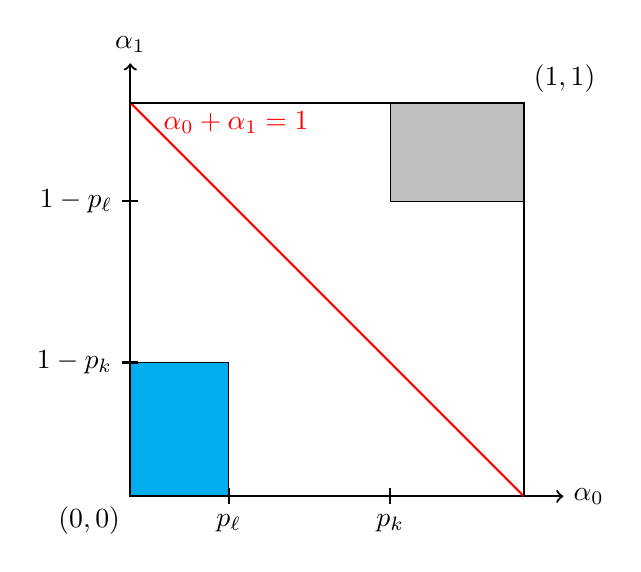
\begin{tikzpicture}[scale=5]
    \draw [fill = lightgray] (0.66,0.75) rectangle (1,1);
    \draw [fill = cyan] (0,0) rectangle (0.25, 0.34);
    \draw [thick, <->] (0,1.1)
    node[above] {$\alpha_1$} -- (0,0) 
    node [below left] {$(0,0)$} -- (1.1,0) 
    node [right] {$\alpha_0$};
    \draw [thick] (0.25,0.02) -- (0.25,-0.02) node [below] {$p_\ell$}; 
    \draw [thick] (0.02,0.75) -- (-0.02,0.75) node [left] {$1 - p_\ell$}; 
    \draw [thick] (0.66,0.02) -- (0.66,-0.02) node [below] {$p_k$}; 
    \draw [thick] (0.02,0.34) -- (-0.02,0.34) node [left] {$1 - p_k$}; 
    \draw [thick, red] (0,1) to (1,0); 
    \node [right, red] at (0.06,0.95) {$\alpha_0 + \alpha_1 = 1$};
    \draw [thick] (0,1) -- (1,1) -- (1,0);
    \node [above right] at (1,1) {$(1,1)$};
    \end{tikzpicture}
\end{figure}
\end{frame}
%%%%%%%%%%%%%%%%%%%%%%%%%%%%%%%%%%%%%%
\begin{frame}
  \frametitle{What does IV estimate under mis-classification?}
  \begin{block}{Unobserved}
  \[
    \beta(\mathbf{x}) = \frac{\mathbb{E}[y|\mathbf{x},z=1] - \mathbb{E}[y|\mathbf{x},z=0]}{p^*_1(\mathbf{x}) - p^*_0(\mathbf{x})} 
  \]
  \end{block}

  \begin{block}{Wald (Observed)}
    \vspace{-1em}
    \small
    \[
      \frac{\mathbb{E}[y|\mathbf{x},z=1] - \mathbb{E}[y|\mathbf{x},z=0]}{p_1(\mathbf{x}) - p_0(\mathbf{x})} = \beta(\mathbf{x})\left[ \frac{p_1^*(\mathbf{x}) - p_0^*(\mathbf{x})}{p_1(\mathbf{x}) - p_0(\mathbf{x})} \right] = \alert{\frac{\beta(\mathbf{x})}{1 - \alpha_0(\mathbf{x}) - \alpha_1(\mathbf{x})} }
    \]
   
    \vspace{2em}
    \scriptsize
    \[
      \boxed{p_1^*(\mathbf{x}) - p_0^*(\mathbf{x}) = \frac{p_1(\mathbf{x}) - \alpha_0(\mathbf{x})}{1 - \alpha_0 - \alpha_1(\mathbf{x})} -   \frac{p_0(\mathbf{x}) - \alpha_0(\mathbf{x})}{1 - \alpha_0 - \alpha_1(\mathbf{x})} = \frac{p_1(\mathbf{x}) - p_0(\mathbf{x})}{1 - \alpha_0(\mathbf{x}) - \alpha_1(\mathbf{x})}}
    \]
  \end{block}
\end{frame}
%%%%%%%%%%%%%%%%%%%%%%%%%%%%%%%%%%%%%%
%\begin{frame}
%  \frametitle{Partial Identification Bounds for $\beta(\mathbf{x})$}
%
%    \footnotesize
%    \[
%      \boxed{ \beta(\mathbf{x}) = \left[ 1 - \alpha_0(\mathbf{x}) - \alpha_1(\mathbf{x}) \right] 
%     \left[\frac{\mathbb{E}\left[y|\mathbf{x},z=1\right] - \mathbb{E}\left[y|\mathbf{x},z=0\right]}{p_1(\mathbf{x}) - p_0(\mathbf{x})}\right] }
%    \]
%
%    \footnotesize
%    \[
%      \boxed{ 0 \leq \alpha_0 \leq \min_k \{p_k(\mathbf{x})\}, \quad 0 \leq \alpha_1 \leq \min_k \{1 - p_k(\mathbf{x})\}}
%    \]
%
%    \normalsize
%    \begin{block}{No Mis-classification}
%      $\alpha_0(\mathbf{x}) =  \alpha_1(\mathbf{x}) = 0 \implies \alert{\beta(\mathbf{x}) = }$ \alert{Wald}
%    \end{block}
%
%    \begin{block}{Maximum Mis-classification}
%      $\alpha_0(\mathbf{x}) = p_{\min}(\mathbf{x}), \, \alpha_1(\mathbf{x}) = 1 - p_{\max}(\mathbf{x})$
%
%      \vspace{-0.5em}
%      \begin{align*}
%        \implies 1 - \alpha_0(\mathbf{x}) - \alpha_1(\mathbf{x}) = p_{\max}(\mathbf{x}) - p_{\min}(\mathbf{x})
%      = |p_1(\mathbf{x}) - p_0(\mathbf{x})|\\
%      \implies \alert{\beta(\mathbf{x}) =\mbox{sign}\left\{ p_1(\mathbf{x}) - p_0(\mathbf{x}) \right\}\times (\mbox{Reduced Form})}
%    \end{align*}
%      
%    \end{block}
%  
%\end{frame}
%%%%%%%%%%%%%%%%%%%%%%%%%%%%%%%%%%%%%%%
%\begin{frame}
%  \frametitle{Partial Identification Bounds for $\beta(\mathbf{x})$}
%
%    \begin{block}{No Mis-classification}
%      $\beta(\mathbf{x}) = $ Wald 
%    \end{block}
%
%    \begin{block}{Maximum Mis-classification}
%      \vspace{-1.5em}
%      \begin{align*}
%        \beta(\mathbf{x}) &=\mbox{sign}\left\{ p_1(\mathbf{x}) - p_0(\mathbf{x}) \right\}\times (\mbox{Reduced Form})\\
%        &=\mbox{sign}\left\{ \mbox{Wald} \right\} \times |\mbox{Reduced Form}|
%      \end{align*}
%      
%      \vspace{1em}
%    \footnotesize Wald $> 0\iff \mbox{sign}\left\{ p_1(\mathbf{x}) - p_0(\mathbf{x}) \right\} = \mbox{sign}\left\{ \mbox{Reduced Form} \right\}$ \\
%    \footnotesize Wald $< 0\iff \mbox{sign}\left\{ p_1(\mathbf{x}) - p_0(\mathbf{x}) \right\} \neq \mbox{sign}\left\{ \mbox{Reduced Form} \right\}$ 
%    \end{block}
%
%    \vspace{1em}
%    \begin{alertblock}{
%        $\beta(\mathbf{x})$ has the same sign as the Wald and its magnitude is between that of Wald and Reduced Form.}
%    \end{alertblock}
%
%\end{frame}
%%%%%%%%%%%%%%%%%%%%%%%%%%%%%%%%%%%%%%
\begin{frame}
  \frametitle{Partial Identification Bounds for $\beta(\mathbf{x})$}

  \begin{block}{Known Result}
    \begin{itemize}
      \item $\beta(\mathbf{x})$ is between Wald and Reduced form; same sign as Wald.
      \item Doesn't rely on non-differential assumption or additive sep.\
      \item Frazis \& Loewenstein (2003), Ura (2016), \ldots
    \end{itemize}
    \end{block}

    \begin{alertblock}{Non-differential Assumption}
      \begin{itemize}
        \item $\mathbb{E}[\varepsilon|\mathbf{x},T^*,T,z] = \mathbb{E}[\varepsilon|\mathbf{x},T^*,z]$
        \item Used in literature to identify $\beta(\mathbf{x})$ when $T^*$ is exogenous. 
        \item Does it restrict the identified set when $T^*$ is \alert{endogenous}? 
        %\item Is $\beta(\mathbf{x})$ identified under the baseline assumptions?
      \end{itemize}
    \end{alertblock}

    \note{Answer turns out to be yes. Now talk about our 2nd contribution: deriving the so-called ``sharp'' identified set }

\end{frame}
%%%%%%%%%%%%%%%%%%%%%%%%%%%%%%%%%%%%%%%%%%%%%%%%%%%%
\begin{frame}[t]
  \frametitle{Restrictions from Non-differential Mis-classification?}
  \framesubtitle{(Suppress $\mathbf{x}$ for simplicity)}

  \footnotesize

  \begin{block}{Notation}
    \begin{itemize}
      \item $r_{tk} \equiv \mathbb{P}(T^*=1|T=t,z=k)$, function of $(\alpha_0, \alpha_1)$ and observables only 
      \item $z_k$ is shorthand for $z =k$\\
    \end{itemize}
  \end{block}

  \begin{block}{Iterated Expectations over $T^*$}
    \vspace{-1em}
  \begin{align*}
    \mathbb{E}(y|T=0,z_k) &= (1 - r_{0k})\mathbb{E}(y|T^*=0,T=0,z_k) + r_{0k}\mathbb{E}(y|T^*=1,T=0,z_k)\\
    \mathbb{E}(y|T=1,z_k) &= (1 - r_{1k}) \mathbb{E}(y|T^*=0,T=1,z_k) + r_{1k}\mathbb{E}(y|T^*=1,T=1,z_k)
  \end{align*}
  \end{block}

\end{frame}
%%%%%%%%%%%%%%%%%%%%%%%%%%%%%%%%%%%%%%%%%%%%%%%%%%%%
\begin{frame}[t,noframenumbering]
  \frametitle{Restrictions from Non-differential Mis-classification?}
  \framesubtitle{(Suppress $\mathbf{x}$ for simplicity)}

  \footnotesize

  \begin{block}{Notation}
    \begin{itemize}
      \item $r_{tk} \equiv \mathbb{P}(T^*=1|T=t,z=k)$, function of $(\alpha_0, \alpha_1)$ and observables only 
      \item $z_k$ is shorthand for $z =k$\\
    \end{itemize}
  \end{block}
  
  \begin{block}{Adding Non-differential Assumption}
    \vspace{-1em}
  \begin{align*}
    \mathbb{E}(y|T=0,z_k) &= (1 - r_{0k})\textcolor{blue}{\mathbb{E}(y|T^*=0,z_k)}\phantom{,T=0} + r_{0k}\textcolor{red}{\mathbb{E}(y|T^*=1,z_k)}\phantom{,T=0}\\
    \mathbb{E}(y|T=1,z_k) &= (1 - r_{1k}) \textcolor{blue}{\mathbb{E}(y|T^*=0,z_k)}\phantom{,T=1} + r_{1k}\textcolor{red}{\mathbb{E}(y|T^*=1,z_k)}\phantom{,T=1}
  \end{align*}

  \vspace{1em}
  \fbox{2 equations in 2 unknowns $\Rightarrow$ solve for $\mathbb{E}(y|T^*=t^*,z=k)$ given $(\alpha_0, \alpha_1)$.}

  \end{block}

\end{frame}
%%%%%%%%%%%%%%%%%%%%%%%%%%%%%%%%%%%%%%%%%%%%%%%%
\begin{frame}
  \frametitle{Restrictions from Non-differential Mis-classification?}

  \begin{block}{Law of Total Probability}
    \vspace{-1.5em}
  \[
    \boxed{\textcolor{blue}{F_{tk}} = (1 - r_{tk}) \alert{F^{0}_{tk}} + r_{tk}\alert{F^{1}_{tk}}}
  \]
  \scriptsize

  \vspace{-1em}
    \begin{align*}
    \textcolor{blue}{F_{tk}} &\equiv \mbox{\textcolor{blue}{Observed} CDF: } y|(T=t,z=k) \\
    \alert{F^{t^*}_{tk}} &\equiv \mbox{\alert{Unobserved} CDF: } y|(T^*=t^*,T=t,z=k)
    \end{align*}
  \end{block}

  \begin{block}{Previous Slide}
    \begin{itemize} 
    \small
      \item $r_{tk}$ observable given $(\alpha_0, \alpha_1)$
      \item $\mathbb{E}(y|T^*,T,z) = \mathbb{E}(y|T^*,z)$ observable given $(\alpha_0, \alpha_1)$
    \end{itemize}
    
  \end{block}

  \begin{alertblock}{Key Question}
    \small
  Given $(\alpha_0, \alpha_1)$ can we always find $(F_{tk}^0, F_{tk}^1)$ to satisfy the mixture model? 
  \end{alertblock}
    



\end{frame}
%%%%%%%%%%%%%%%%%%%%%%%%%%%%%%%%%%%%%%%%%%%%%%%%%%%%
\begin{frame}
  \frametitle{Restrictions from Non-differential Mis-classification?}

  \begin{block}{Equivalent Problem}
    \small
    Given a specified CDF $F$, for what values of $p$ and $\mu$ do there exist valid CDFs $(G,H)$ with $F = (1 - p) G + p H$ and $\mu = \mbox{mean}(H)$? 
\end{block}

%  \begin{block}{Equivalent Problem}
%    Given a specified CDF $\textcolor{red}{F}$, probability $\textcolor{red}{p}$ and mean $\textcolor{red}{\mu}$, do there exist valid CDFs $\textcolor{red}{(G,H)}$ with $\textcolor{red}{F = (1 - p) G + p H}$ and $\textcolor{red}{\mu = \mbox{mean}(H)}$? 
%  \end{block}

%\begin{block}{Solve to Eliminate $G$}
%  \small
%  $G = (F - p H) / (1 - p)$
%\end{block}

\begin{block}{Valid CDFS}
  \vspace{-1em}
  \scriptsize
  \begin{align*}
    0 \leq H \leq 1 & \\
    0 \leq G \leq 1 & \quad \iff \quad [F - (1 - p)]/p \leq H \leq F/p
  \end{align*}

  \normalsize
  \[
    \alert{\boxed{\max\left\{ 0, \, \frac{F(x)}{p} - \frac{1-p}{p} \right\}\leq H(x) \leq \min\left\{ 1, \frac{F(x)}{p} \right\}}}
  \]
\end{block}

\note{Explain how we solve to eliminate $G$ and get conditions on $H$ only!}


\end{frame}
%%%%%%%%%%%%%%%%%%%%%%%%%%%%%%%%%%%%%%%%%%%%%%%%%%%%
\begin{frame}
  \frametitle{Restrictions from Non-differential Mis-classification?}
  \begin{block}{Notation}
    \footnotesize
    \vspace{-1em}
    \[
      \overline{H} \equiv \max\left\{ 0, \, \frac{F(x)}{p} - \frac{1-p}{p} \right\}, \quad
      \underline{H} \equiv \min\left\{ 1, \frac{F(x)}{p} \right\}
    \]
  \end{block}
  
  \begin{alertblock}{1\textsuperscript{st} Order Stochastic Dominance}
    \vspace{-1em}
      \[
        \overline{H}(x) \leq H(x) \leq \underline{H}(x) \quad \mbox{for all } x
      \]

      \vspace{-1em}
      \[
        \alert{\implies \underbrace{\int_{\mathbb{R}} x\, \underline{H}(dx)}_{\underline{\mu}(p,F)} \leq \underbrace{\int_{\mathbb{R}} x\, H(dx)}_{\mu} \leq \underbrace{\int_{\mathbb{R}} x\, \overline{H}(dx)}_{\overline{\mu}(p,F)}}
      \]
  \end{alertblock}

  \note{Explain the somewhat odd-looking convention for $\underline{H}$ and $\overline{H}$. Constraint from preceding slide is a stochastic dominance relationship. It implies an inequality for means.}
\end{frame}
%%%%%%%%%%%%%%%%%%%%%%%%%%%%%%%%%%%%%%%%%%%%%%%%%%%%
\begin{frame}

\begin{figure}[h]
  \centering
\resizebox{0.85\textwidth}{!}{%
  % Created by tikzDevice version 0.10.1 on 2018-01-15 17:35:19
% !TEX encoding = UTF-8 Unicode
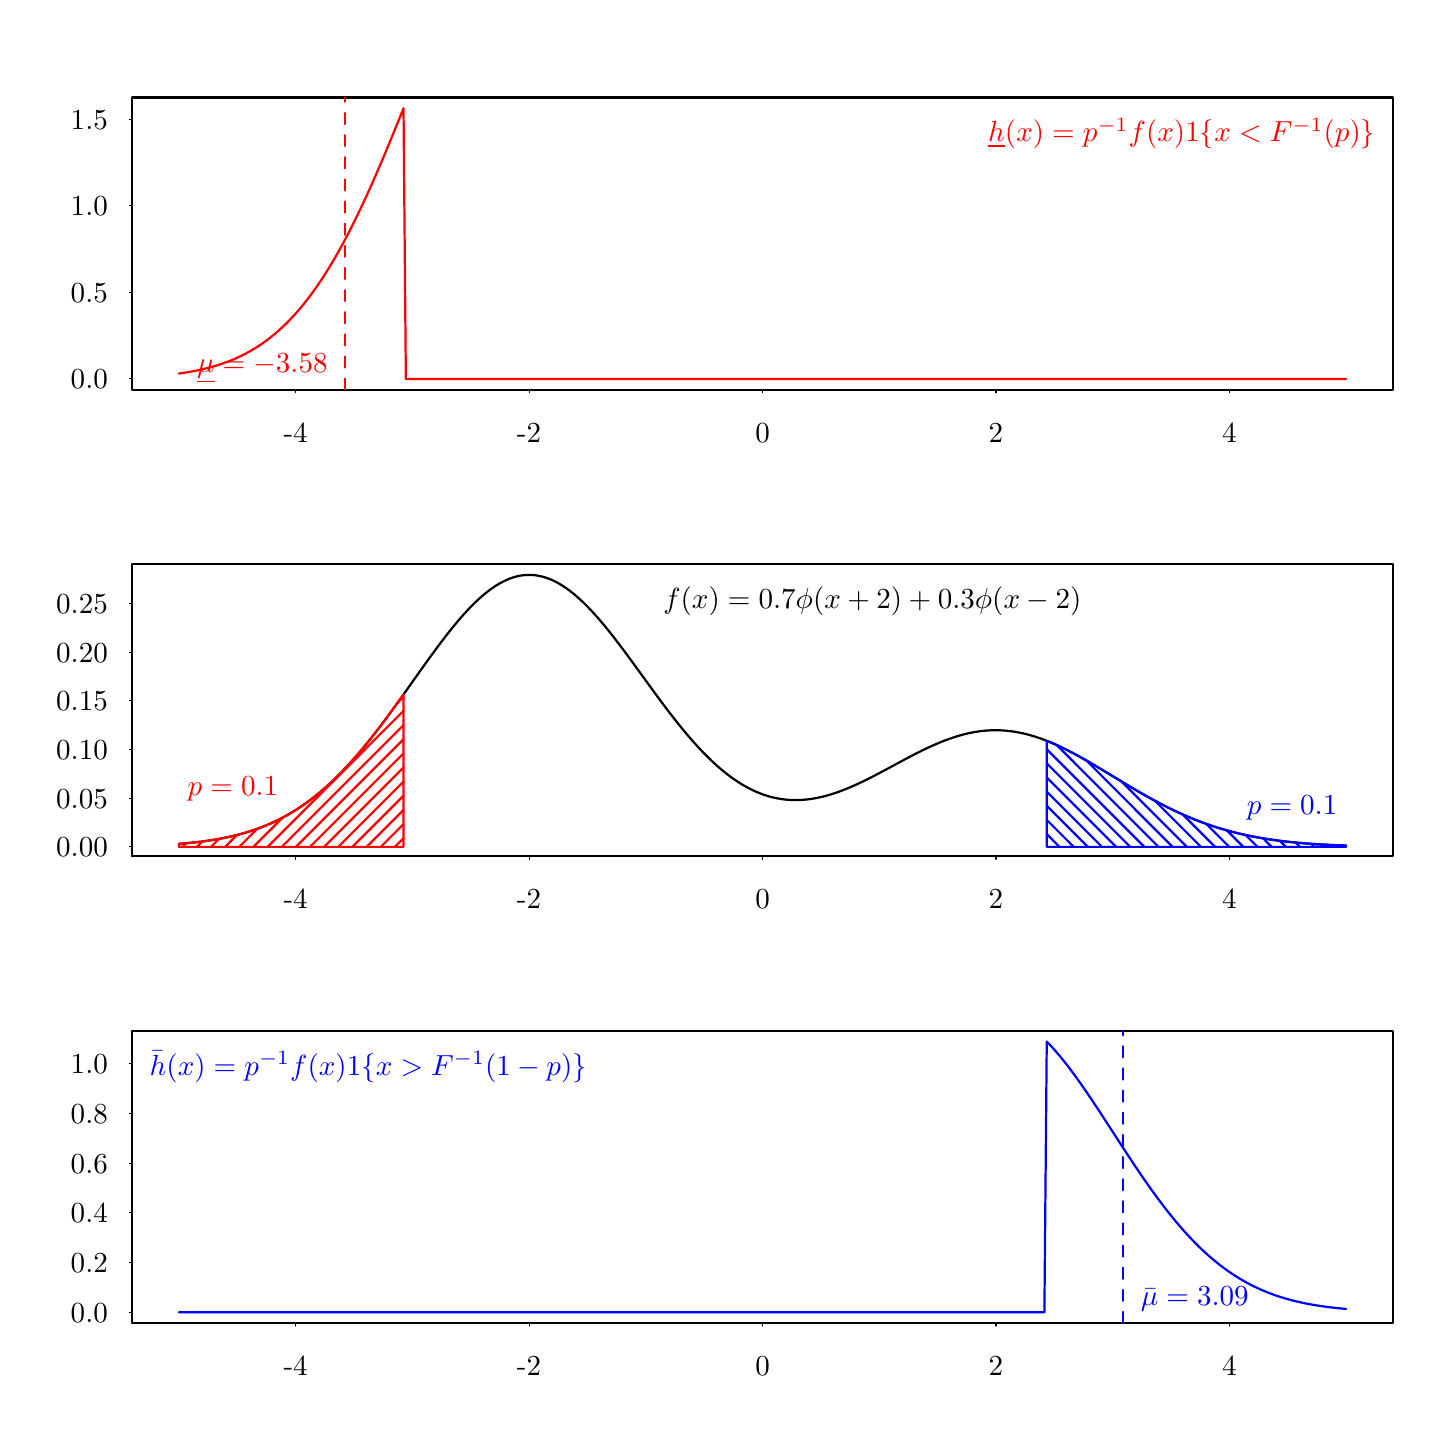
\begin{tikzpicture}[x=1pt,y=1pt]
\definecolor{fillColor}{RGB}{255,255,255}
\path[use as bounding box,fill=fillColor,fill opacity=0.00] (0,0) rectangle (505.89,505.89);
\begin{scope}
\path[clip] ( 37.80,375.06) rectangle (493.29,480.69);
\definecolor{drawColor}{RGB}{255,0,0}

\path[draw=drawColor,line width= 0.8pt,line join=round,line cap=round] ( 54.67,380.91) --
	( 55.52,381.03) --
	( 56.36,381.16) --
	( 57.21,381.29) --
	( 58.05,381.43) --
	( 58.90,381.58) --
	( 59.74,381.73) --
	( 60.59,381.90) --
	( 61.43,382.07) --
	( 62.28,382.25) --
	( 63.12,382.44) --
	( 63.97,382.64) --
	( 64.81,382.85) --
	( 65.66,383.07) --
	( 66.50,383.30) --
	( 67.35,383.54) --
	( 68.19,383.79) --
	( 69.04,384.06) --
	( 69.88,384.33) --
	( 70.73,384.62) --
	( 71.57,384.93) --
	( 72.42,385.24) --
	( 73.26,385.57) --
	( 74.11,385.92) --
	( 74.95,386.28) --
	( 75.80,386.66) --
	( 76.64,387.05) --
	( 77.49,387.46) --
	( 78.34,387.89) --
	( 79.18,388.33) --
	( 80.03,388.80) --
	( 80.87,389.28) --
	( 81.72,389.78) --
	( 82.56,390.30) --
	( 83.41,390.84) --
	( 84.25,391.40) --
	( 85.10,391.99) --
	( 85.94,392.59) --
	( 86.79,393.22) --
	( 87.63,393.87) --
	( 88.48,394.55) --
	( 89.32,395.24) --
	( 90.17,395.97) --
	( 91.01,396.71) --
	( 91.86,397.49) --
	( 92.70,398.29) --
	( 93.55,399.11) --
	( 94.39,399.96) --
	( 95.24,400.84) --
	( 96.08,401.75) --
	( 96.93,402.69) --
	( 97.77,403.65) --
	( 98.62,404.64) --
	( 99.47,405.66) --
	(100.31,406.72) --
	(101.16,407.80) --
	(102.00,408.91) --
	(102.85,410.05) --
	(103.69,411.22) --
	(104.54,412.42) --
	(105.38,413.66) --
	(106.23,414.92) --
	(107.07,416.22) --
	(107.92,417.55) --
	(108.76,418.91) --
	(109.61,420.30) --
	(110.45,421.72) --
	(111.30,423.17) --
	(112.14,424.65) --
	(112.99,426.17) --
	(113.83,427.71) --
	(114.68,429.29) --
	(115.52,430.89) --
	(116.37,432.53) --
	(117.21,434.19) --
	(118.06,435.89) --
	(118.90,437.61) --
	(119.75,439.36) --
	(120.59,441.13) --
	(121.44,442.94) --
	(122.29,444.77) --
	(123.13,446.62) --
	(123.98,448.50) --
	(124.82,450.40) --
	(125.67,452.32) --
	(126.51,454.27) --
	(127.36,456.24) --
	(128.20,458.22) --
	(129.05,460.23) --
	(129.89,462.25) --
	(130.74,464.29) --
	(131.58,466.34) --
	(132.43,468.41) --
	(133.27,470.48) --
	(134.12,472.57) --
	(134.96,474.67) --
	(135.81,476.78) --
	(136.65,378.97) --
	(137.50,378.97) --
	(138.34,378.97) --
	(139.19,378.97) --
	(140.03,378.97) --
	(140.88,378.97) --
	(141.72,378.97) --
	(142.57,378.97) --
	(143.41,378.97) --
	(144.26,378.97) --
	(145.11,378.97) --
	(145.95,378.97) --
	(146.80,378.97) --
	(147.64,378.97) --
	(148.49,378.97) --
	(149.33,378.97) --
	(150.18,378.97) --
	(151.02,378.97) --
	(151.87,378.97) --
	(152.71,378.97) --
	(153.56,378.97) --
	(154.40,378.97) --
	(155.25,378.97) --
	(156.09,378.97) --
	(156.94,378.97) --
	(157.78,378.97) --
	(158.63,378.97) --
	(159.47,378.97) --
	(160.32,378.97) --
	(161.16,378.97) --
	(162.01,378.97) --
	(162.85,378.97) --
	(163.70,378.97) --
	(164.54,378.97) --
	(165.39,378.97) --
	(166.24,378.97) --
	(167.08,378.97) --
	(167.93,378.97) --
	(168.77,378.97) --
	(169.62,378.97) --
	(170.46,378.97) --
	(171.31,378.97) --
	(172.15,378.97) --
	(173.00,378.97) --
	(173.84,378.97) --
	(174.69,378.97) --
	(175.53,378.97) --
	(176.38,378.97) --
	(177.22,378.97) --
	(178.07,378.97) --
	(178.91,378.97) --
	(179.76,378.97) --
	(180.60,378.97) --
	(181.45,378.97) --
	(182.29,378.97) --
	(183.14,378.97) --
	(183.98,378.97) --
	(184.83,378.97) --
	(185.67,378.97) --
	(186.52,378.97) --
	(187.36,378.97) --
	(188.21,378.97) --
	(189.06,378.97) --
	(189.90,378.97) --
	(190.75,378.97) --
	(191.59,378.97) --
	(192.44,378.97) --
	(193.28,378.97) --
	(194.13,378.97) --
	(194.97,378.97) --
	(195.82,378.97) --
	(196.66,378.97) --
	(197.51,378.97) --
	(198.35,378.97) --
	(199.20,378.97) --
	(200.04,378.97) --
	(200.89,378.97) --
	(201.73,378.97) --
	(202.58,378.97) --
	(203.42,378.97) --
	(204.27,378.97) --
	(205.11,378.97) --
	(205.96,378.97) --
	(206.80,378.97) --
	(207.65,378.97) --
	(208.49,378.97) --
	(209.34,378.97) --
	(210.19,378.97) --
	(211.03,378.97) --
	(211.88,378.97) --
	(212.72,378.97) --
	(213.57,378.97) --
	(214.41,378.97) --
	(215.26,378.97) --
	(216.10,378.97) --
	(216.95,378.97) --
	(217.79,378.97) --
	(218.64,378.97) --
	(219.48,378.97) --
	(220.33,378.97) --
	(221.17,378.97) --
	(222.02,378.97) --
	(222.86,378.97) --
	(223.71,378.97) --
	(224.55,378.97) --
	(225.40,378.97) --
	(226.24,378.97) --
	(227.09,378.97) --
	(227.93,378.97) --
	(228.78,378.97) --
	(229.62,378.97) --
	(230.47,378.97) --
	(231.31,378.97) --
	(232.16,378.97) --
	(233.01,378.97) --
	(233.85,378.97) --
	(234.70,378.97) --
	(235.54,378.97) --
	(236.39,378.97) --
	(237.23,378.97) --
	(238.08,378.97) --
	(238.92,378.97) --
	(239.77,378.97) --
	(240.61,378.97) --
	(241.46,378.97) --
	(242.30,378.97) --
	(243.15,378.97) --
	(243.99,378.97) --
	(244.84,378.97) --
	(245.68,378.97) --
	(246.53,378.97) --
	(247.37,378.97) --
	(248.22,378.97) --
	(249.06,378.97) --
	(249.91,378.97) --
	(250.75,378.97) --
	(251.60,378.97) --
	(252.44,378.97) --
	(253.29,378.97) --
	(254.13,378.97) --
	(254.98,378.97) --
	(255.83,378.97) --
	(256.67,378.97) --
	(257.52,378.97) --
	(258.36,378.97) --
	(259.21,378.97) --
	(260.05,378.97) --
	(260.90,378.97) --
	(261.74,378.97) --
	(262.59,378.97) --
	(263.43,378.97) --
	(264.28,378.97) --
	(265.12,378.97) --
	(265.97,378.97) --
	(266.81,378.97) --
	(267.66,378.97) --
	(268.50,378.97) --
	(269.35,378.97) --
	(270.19,378.97) --
	(271.04,378.97) --
	(271.88,378.97) --
	(272.73,378.97) --
	(273.57,378.97) --
	(274.42,378.97) --
	(275.26,378.97) --
	(276.11,378.97) --
	(276.96,378.97) --
	(277.80,378.97) --
	(278.65,378.97) --
	(279.49,378.97) --
	(280.34,378.97) --
	(281.18,378.97) --
	(282.03,378.97) --
	(282.87,378.97) --
	(283.72,378.97) --
	(284.56,378.97) --
	(285.41,378.97) --
	(286.25,378.97) --
	(287.10,378.97) --
	(287.94,378.97) --
	(288.79,378.97) --
	(289.63,378.97) --
	(290.48,378.97) --
	(291.32,378.97) --
	(292.17,378.97) --
	(293.01,378.97) --
	(293.86,378.97) --
	(294.70,378.97) --
	(295.55,378.97) --
	(296.39,378.97) --
	(297.24,378.97) --
	(298.08,378.97) --
	(298.93,378.97) --
	(299.78,378.97) --
	(300.62,378.97) --
	(301.47,378.97) --
	(302.31,378.97) --
	(303.16,378.97) --
	(304.00,378.97) --
	(304.85,378.97) --
	(305.69,378.97) --
	(306.54,378.97) --
	(307.38,378.97) --
	(308.23,378.97) --
	(309.07,378.97) --
	(309.92,378.97) --
	(310.76,378.97) --
	(311.61,378.97) --
	(312.45,378.97) --
	(313.30,378.97) --
	(314.14,378.97) --
	(314.99,378.97) --
	(315.83,378.97) --
	(316.68,378.97) --
	(317.52,378.97) --
	(318.37,378.97) --
	(319.21,378.97) --
	(320.06,378.97) --
	(320.90,378.97) --
	(321.75,378.97) --
	(322.60,378.97) --
	(323.44,378.97) --
	(324.29,378.97) --
	(325.13,378.97) --
	(325.98,378.97) --
	(326.82,378.97) --
	(327.67,378.97) --
	(328.51,378.97) --
	(329.36,378.97) --
	(330.20,378.97) --
	(331.05,378.97) --
	(331.89,378.97) --
	(332.74,378.97) --
	(333.58,378.97) --
	(334.43,378.97) --
	(335.27,378.97) --
	(336.12,378.97) --
	(336.96,378.97) --
	(337.81,378.97) --
	(338.65,378.97) --
	(339.50,378.97) --
	(340.34,378.97) --
	(341.19,378.97) --
	(342.03,378.97) --
	(342.88,378.97) --
	(343.73,378.97) --
	(344.57,378.97) --
	(345.42,378.97) --
	(346.26,378.97) --
	(347.11,378.97) --
	(347.95,378.97) --
	(348.80,378.97) --
	(349.64,378.97) --
	(350.49,378.97) --
	(351.33,378.97) --
	(352.18,378.97) --
	(353.02,378.97) --
	(353.87,378.97) --
	(354.71,378.97) --
	(355.56,378.97) --
	(356.40,378.97) --
	(357.25,378.97) --
	(358.09,378.97) --
	(358.94,378.97) --
	(359.78,378.97) --
	(360.63,378.97) --
	(361.47,378.97) --
	(362.32,378.97) --
	(363.16,378.97) --
	(364.01,378.97) --
	(364.85,378.97) --
	(365.70,378.97) --
	(366.55,378.97) --
	(367.39,378.97) --
	(368.24,378.97) --
	(369.08,378.97) --
	(369.93,378.97) --
	(370.77,378.97) --
	(371.62,378.97) --
	(372.46,378.97) --
	(373.31,378.97) --
	(374.15,378.97) --
	(375.00,378.97) --
	(375.84,378.97) --
	(376.69,378.97) --
	(377.53,378.97) --
	(378.38,378.97) --
	(379.22,378.97) --
	(380.07,378.97) --
	(380.91,378.97) --
	(381.76,378.97) --
	(382.60,378.97) --
	(383.45,378.97) --
	(384.29,378.97) --
	(385.14,378.97) --
	(385.98,378.97) --
	(386.83,378.97) --
	(387.68,378.97) --
	(388.52,378.97) --
	(389.37,378.97) --
	(390.21,378.97) --
	(391.06,378.97) --
	(391.90,378.97) --
	(392.75,378.97) --
	(393.59,378.97) --
	(394.44,378.97) --
	(395.28,378.97) --
	(396.13,378.97) --
	(396.97,378.97) --
	(397.82,378.97) --
	(398.66,378.97) --
	(399.51,378.97) --
	(400.35,378.97) --
	(401.20,378.97) --
	(402.04,378.97) --
	(402.89,378.97) --
	(403.73,378.97) --
	(404.58,378.97) --
	(405.42,378.97) --
	(406.27,378.97) --
	(407.11,378.97) --
	(407.96,378.97) --
	(408.80,378.97) --
	(409.65,378.97) --
	(410.50,378.97) --
	(411.34,378.97) --
	(412.19,378.97) --
	(413.03,378.97) --
	(413.88,378.97) --
	(414.72,378.97) --
	(415.57,378.97) --
	(416.41,378.97) --
	(417.26,378.97) --
	(418.10,378.97) --
	(418.95,378.97) --
	(419.79,378.97) --
	(420.64,378.97) --
	(421.48,378.97) --
	(422.33,378.97) --
	(423.17,378.97) --
	(424.02,378.97) --
	(424.86,378.97) --
	(425.71,378.97) --
	(426.55,378.97) --
	(427.40,378.97) --
	(428.24,378.97) --
	(429.09,378.97) --
	(429.93,378.97) --
	(430.78,378.97) --
	(431.62,378.97) --
	(432.47,378.97) --
	(433.32,378.97) --
	(434.16,378.97) --
	(435.01,378.97) --
	(435.85,378.97) --
	(436.70,378.97) --
	(437.54,378.97) --
	(438.39,378.97) --
	(439.23,378.97) --
	(440.08,378.97) --
	(440.92,378.97) --
	(441.77,378.97) --
	(442.61,378.97) --
	(443.46,378.97) --
	(444.30,378.97) --
	(445.15,378.97) --
	(445.99,378.97) --
	(446.84,378.97) --
	(447.68,378.97) --
	(448.53,378.97) --
	(449.37,378.97) --
	(450.22,378.97) --
	(451.06,378.97) --
	(451.91,378.97) --
	(452.75,378.97) --
	(453.60,378.97) --
	(454.45,378.97) --
	(455.29,378.97) --
	(456.14,378.97) --
	(456.98,378.97) --
	(457.83,378.97) --
	(458.67,378.97) --
	(459.52,378.97) --
	(460.36,378.97) --
	(461.21,378.97) --
	(462.05,378.97) --
	(462.90,378.97) --
	(463.74,378.97) --
	(464.59,378.97) --
	(465.43,378.97) --
	(466.28,378.97) --
	(467.12,378.97) --
	(467.97,378.97) --
	(468.81,378.97) --
	(469.66,378.97) --
	(470.50,378.97) --
	(471.35,378.97) --
	(472.19,378.97) --
	(473.04,378.97) --
	(473.88,378.97) --
	(474.73,378.97) --
	(475.57,378.97) --
	(476.42,378.97);
\end{scope}
\begin{scope}
\path[clip] (  0.00,  0.00) rectangle (505.89,505.89);
\definecolor{drawColor}{RGB}{0,0,0}

\path[draw=drawColor,line width= 0.4pt,line join=round,line cap=round] ( 96.84,375.06) -- (434.25,375.06);

\path[draw=drawColor,line width= 0.4pt,line join=round,line cap=round] ( 96.84,375.06) -- ( 96.84,374.00);

\path[draw=drawColor,line width= 0.4pt,line join=round,line cap=round] (181.19,375.06) -- (181.19,374.00);

\path[draw=drawColor,line width= 0.4pt,line join=round,line cap=round] (265.54,375.06) -- (265.54,374.00);

\path[draw=drawColor,line width= 0.4pt,line join=round,line cap=round] (349.89,375.06) -- (349.89,374.00);

\path[draw=drawColor,line width= 0.4pt,line join=round,line cap=round] (434.25,375.06) -- (434.25,374.00);

\node[text=drawColor,anchor=base,inner sep=0pt, outer sep=0pt, scale=  1.05] at ( 96.84,356.16) {-4};

\node[text=drawColor,anchor=base,inner sep=0pt, outer sep=0pt, scale=  1.05] at (181.19,356.16) {-2};

\node[text=drawColor,anchor=base,inner sep=0pt, outer sep=0pt, scale=  1.05] at (265.54,356.16) {0};

\node[text=drawColor,anchor=base,inner sep=0pt, outer sep=0pt, scale=  1.05] at (349.89,356.16) {2};

\node[text=drawColor,anchor=base,inner sep=0pt, outer sep=0pt, scale=  1.05] at (434.25,356.16) {4};

\path[draw=drawColor,line width= 0.4pt,line join=round,line cap=round] ( 37.80,378.97) -- ( 37.80,472.71);

\path[draw=drawColor,line width= 0.4pt,line join=round,line cap=round] ( 37.80,378.97) -- ( 36.74,378.97);

\path[draw=drawColor,line width= 0.4pt,line join=round,line cap=round] ( 37.80,410.22) -- ( 36.74,410.22);

\path[draw=drawColor,line width= 0.4pt,line join=round,line cap=round] ( 37.80,441.47) -- ( 36.74,441.47);

\path[draw=drawColor,line width= 0.4pt,line join=round,line cap=round] ( 37.80,472.71) -- ( 36.74,472.71);

\node[text=drawColor,anchor=base east,inner sep=0pt, outer sep=0pt, scale=  1.05] at ( 28.98,375.36) {0.0};

\node[text=drawColor,anchor=base east,inner sep=0pt, outer sep=0pt, scale=  1.05] at ( 28.98,406.60) {0.5};

\node[text=drawColor,anchor=base east,inner sep=0pt, outer sep=0pt, scale=  1.05] at ( 28.98,437.85) {1.0};

\node[text=drawColor,anchor=base east,inner sep=0pt, outer sep=0pt, scale=  1.05] at ( 28.98,469.10) {1.5};

\path[draw=drawColor,line width= 0.8pt,line join=round,line cap=round] ( 37.80,375.06) --
	(493.29,375.06) --
	(493.29,480.69) --
	( 37.80,480.69) --
	( 37.80,375.06);
\end{scope}
\begin{scope}
\path[clip] ( 37.80,375.06) rectangle (493.29,480.69);
\definecolor{drawColor}{RGB}{255,0,0}

\node[text=drawColor,anchor=base east,inner sep=0pt, outer sep=0pt, scale=  1.05] at (486.99,464.59) {$\underline{h}(x) = p^{-1}f(x) 1\{x < F^{-1}(p)\}$};

\path[draw=drawColor,line width= 0.8pt,dash pattern=on 4pt off 4pt ,line join=round,line cap=round] (114.67,375.06) -- (114.67,480.69);

\node[text=drawColor,anchor=base east,inner sep=0pt, outer sep=0pt, scale=  1.05] at (108.37,381.45) {$\underline{\mu} = -3.58$};
\end{scope}
\begin{scope}
\path[clip] ( 37.80,206.43) rectangle (493.29,312.06);
\definecolor{drawColor}{RGB}{0,0,0}

\path[draw=drawColor,line width= 0.8pt,line join=round,line cap=round] ( 54.67,210.97) --
	( 55.52,211.03) --
	( 56.36,211.10) --
	( 57.21,211.18) --
	( 58.05,211.26) --
	( 58.90,211.34) --
	( 59.74,211.43) --
	( 60.59,211.52) --
	( 61.43,211.62) --
	( 62.28,211.72) --
	( 63.12,211.83) --
	( 63.97,211.94) --
	( 64.81,212.06) --
	( 65.66,212.18) --
	( 66.50,212.31) --
	( 67.35,212.45) --
	( 68.19,212.59) --
	( 69.04,212.74) --
	( 69.88,212.89) --
	( 70.73,213.06) --
	( 71.57,213.23) --
	( 72.42,213.41) --
	( 73.26,213.59) --
	( 74.11,213.79) --
	( 74.95,213.99) --
	( 75.80,214.20) --
	( 76.64,214.42) --
	( 77.49,214.65) --
	( 78.34,214.90) --
	( 79.18,215.15) --
	( 80.03,215.41) --
	( 80.87,215.68) --
	( 81.72,215.96) --
	( 82.56,216.25) --
	( 83.41,216.56) --
	( 84.25,216.87) --
	( 85.10,217.20) --
	( 85.94,217.54) --
	( 86.79,217.90) --
	( 87.63,218.26) --
	( 88.48,218.64) --
	( 89.32,219.04) --
	( 90.17,219.44) --
	( 91.01,219.86) --
	( 91.86,220.30) --
	( 92.70,220.75) --
	( 93.55,221.21) --
	( 94.39,221.69) --
	( 95.24,222.19) --
	( 96.08,222.70) --
	( 96.93,223.23) --
	( 97.77,223.77) --
	( 98.62,224.33) --
	( 99.47,224.90) --
	(100.31,225.49) --
	(101.16,226.10) --
	(102.00,226.73) --
	(102.85,227.37) --
	(103.69,228.03) --
	(104.54,228.71) --
	(105.38,229.40) --
	(106.23,230.12) --
	(107.07,230.85) --
	(107.92,231.59) --
	(108.76,232.36) --
	(109.61,233.14) --
	(110.45,233.94) --
	(111.30,234.76) --
	(112.14,235.59) --
	(112.99,236.45) --
	(113.83,237.32) --
	(114.68,238.20) --
	(115.52,239.11) --
	(116.37,240.03) --
	(117.21,240.97) --
	(118.06,241.92) --
	(118.90,242.89) --
	(119.75,243.87) --
	(120.59,244.87) --
	(121.44,245.89) --
	(122.29,246.92) --
	(123.13,247.96) --
	(123.98,249.02) --
	(124.82,250.09) --
	(125.67,251.17) --
	(126.51,252.27) --
	(127.36,253.38) --
	(128.20,254.50) --
	(129.05,255.62) --
	(129.89,256.76) --
	(130.74,257.91) --
	(131.58,259.07) --
	(132.43,260.23) --
	(133.27,261.40) --
	(134.12,262.58) --
	(134.96,263.76) --
	(135.81,264.94) --
	(136.65,266.13) --
	(137.50,267.32) --
	(138.34,268.52) --
	(139.19,269.71) --
	(140.03,270.91) --
	(140.88,272.10) --
	(141.72,273.29) --
	(142.57,274.48) --
	(143.41,275.66) --
	(144.26,276.84) --
	(145.11,278.01) --
	(145.95,279.18) --
	(146.80,280.33) --
	(147.64,281.48) --
	(148.49,282.61) --
	(149.33,283.74) --
	(150.18,284.85) --
	(151.02,285.95) --
	(151.87,287.03) --
	(152.71,288.10) --
	(153.56,289.15) --
	(154.40,290.18) --
	(155.25,291.19) --
	(156.09,292.19) --
	(156.94,293.16) --
	(157.78,294.11) --
	(158.63,295.03) --
	(159.47,295.93) --
	(160.32,296.81) --
	(161.16,297.66) --
	(162.01,298.48) --
	(162.85,299.27) --
	(163.70,300.04) --
	(164.54,300.77) --
	(165.39,301.47) --
	(166.24,302.15) --
	(167.08,302.79) --
	(167.93,303.39) --
	(168.77,303.97) --
	(169.62,304.51) --
	(170.46,305.01) --
	(171.31,305.48) --
	(172.15,305.91) --
	(173.00,306.30) --
	(173.84,306.66) --
	(174.69,306.98) --
	(175.53,307.26) --
	(176.38,307.50) --
	(177.22,307.71) --
	(178.07,307.88) --
	(178.91,308.00) --
	(179.76,308.09) --
	(180.60,308.14) --
	(181.45,308.15) --
	(182.29,308.12) --
	(183.14,308.05) --
	(183.98,307.94) --
	(184.83,307.79) --
	(185.67,307.60) --
	(186.52,307.38) --
	(187.36,307.11) --
	(188.21,306.81) --
	(189.06,306.47) --
	(189.90,306.10) --
	(190.75,305.68) --
	(191.59,305.23) --
	(192.44,304.75) --
	(193.28,304.22) --
	(194.13,303.67) --
	(194.97,303.08) --
	(195.82,302.46) --
	(196.66,301.80) --
	(197.51,301.12) --
	(198.35,300.40) --
	(199.20,299.65) --
	(200.04,298.87) --
	(200.89,298.07) --
	(201.73,297.24) --
	(202.58,296.38) --
	(203.42,295.49) --
	(204.27,294.59) --
	(205.11,293.65) --
	(205.96,292.70) --
	(206.80,291.73) --
	(207.65,290.73) --
	(208.49,289.72) --
	(209.34,288.68) --
	(210.19,287.63) --
	(211.03,286.57) --
	(211.88,285.49) --
	(212.72,284.40) --
	(213.57,283.29) --
	(214.41,282.18) --
	(215.26,281.05) --
	(216.10,279.91) --
	(216.95,278.77) --
	(217.79,277.62) --
	(218.64,276.46) --
	(219.48,275.30) --
	(220.33,274.14) --
	(221.17,272.97) --
	(222.02,271.81) --
	(222.86,270.64) --
	(223.71,269.47) --
	(224.55,268.31) --
	(225.40,267.15) --
	(226.24,265.99) --
	(227.09,264.84) --
	(227.93,263.69) --
	(228.78,262.55) --
	(229.62,261.42) --
	(230.47,260.29) --
	(231.31,259.18) --
	(232.16,258.08) --
	(233.01,256.98) --
	(233.85,255.90) --
	(234.70,254.83) --
	(235.54,253.78) --
	(236.39,252.74) --
	(237.23,251.71) --
	(238.08,250.70) --
	(238.92,249.71) --
	(239.77,248.73) --
	(240.61,247.77) --
	(241.46,246.82) --
	(242.30,245.90) --
	(243.15,244.99) --
	(243.99,244.10) --
	(244.84,243.24) --
	(245.68,242.39) --
	(246.53,241.56) --
	(247.37,240.76) --
	(248.22,239.97) --
	(249.06,239.21) --
	(249.91,238.47) --
	(250.75,237.75) --
	(251.60,237.05) --
	(252.44,236.38) --
	(253.29,235.73) --
	(254.13,235.10) --
	(254.98,234.49) --
	(255.83,233.91) --
	(256.67,233.35) --
	(257.52,232.81) --
	(258.36,232.30) --
	(259.21,231.81) --
	(260.05,231.34) --
	(260.90,230.90) --
	(261.74,230.48) --
	(262.59,230.08) --
	(263.43,229.70) --
	(264.28,229.35) --
	(265.12,229.03) --
	(265.97,228.72) --
	(266.81,228.44) --
	(267.66,228.18) --
	(268.50,227.94) --
	(269.35,227.73) --
	(270.19,227.54) --
	(271.04,227.37) --
	(271.88,227.22) --
	(272.73,227.09) --
	(273.57,226.99) --
	(274.42,226.90) --
	(275.26,226.84) --
	(276.11,226.80) --
	(276.96,226.78) --
	(277.80,226.77) --
	(278.65,226.79) --
	(279.49,226.83) --
	(280.34,226.88) --
	(281.18,226.96) --
	(282.03,227.05) --
	(282.87,227.16) --
	(283.72,227.29) --
	(284.56,227.44) --
	(285.41,227.60) --
	(286.25,227.78) --
	(287.10,227.97) --
	(287.94,228.18) --
	(288.79,228.41) --
	(289.63,228.65) --
	(290.48,228.91) --
	(291.32,229.18) --
	(292.17,229.46) --
	(293.01,229.76) --
	(293.86,230.07) --
	(294.70,230.39) --
	(295.55,230.72) --
	(296.39,231.07) --
	(297.24,231.42) --
	(298.08,231.79) --
	(298.93,232.16) --
	(299.78,232.55) --
	(300.62,232.94) --
	(301.47,233.34) --
	(302.31,233.75) --
	(303.16,234.16) --
	(304.00,234.59) --
	(304.85,235.01) --
	(305.69,235.45) --
	(306.54,235.89) --
	(307.38,236.33) --
	(308.23,236.78) --
	(309.07,237.23) --
	(309.92,237.68) --
	(310.76,238.13) --
	(311.61,238.59) --
	(312.45,239.05) --
	(313.30,239.50) --
	(314.14,239.96) --
	(314.99,240.41) --
	(315.83,240.87) --
	(316.68,241.32) --
	(317.52,241.77) --
	(318.37,242.22) --
	(319.21,242.66) --
	(320.06,243.10) --
	(320.90,243.53) --
	(321.75,243.96) --
	(322.60,244.38) --
	(323.44,244.80) --
	(324.29,245.21) --
	(325.13,245.61) --
	(325.98,246.00) --
	(326.82,246.39) --
	(327.67,246.76) --
	(328.51,247.13) --
	(329.36,247.48) --
	(330.20,247.83) --
	(331.05,248.16) --
	(331.89,248.49) --
	(332.74,248.80) --
	(333.58,249.09) --
	(334.43,249.38) --
	(335.27,249.65) --
	(336.12,249.91) --
	(336.96,250.16) --
	(337.81,250.39) --
	(338.65,250.61) --
	(339.50,250.81) --
	(340.34,251.00) --
	(341.19,251.17) --
	(342.03,251.33) --
	(342.88,251.47) --
	(343.73,251.60) --
	(344.57,251.71) --
	(345.42,251.80) --
	(346.26,251.88) --
	(347.11,251.94) --
	(347.95,251.98) --
	(348.80,252.01) --
	(349.64,252.02) --
	(350.49,252.01) --
	(351.33,251.99) --
	(352.18,251.95) --
	(353.02,251.89) --
	(353.87,251.82) --
	(354.71,251.73) --
	(355.56,251.63) --
	(356.40,251.51) --
	(357.25,251.37) --
	(358.09,251.21) --
	(358.94,251.04) --
	(359.78,250.86) --
	(360.63,250.66) --
	(361.47,250.44) --
	(362.32,250.21) --
	(363.16,249.96) --
	(364.01,249.70) --
	(364.85,249.43) --
	(365.70,249.14) --
	(366.55,248.84) --
	(367.39,248.52) --
	(368.24,248.19) --
	(369.08,247.85) --
	(369.93,247.50) --
	(370.77,247.13) --
	(371.62,246.76) --
	(372.46,246.37) --
	(373.31,245.98) --
	(374.15,245.57) --
	(375.00,245.15) --
	(375.84,244.73) --
	(376.69,244.29) --
	(377.53,243.85) --
	(378.38,243.40) --
	(379.22,242.94) --
	(380.07,242.48) --
	(380.91,242.01) --
	(381.76,241.53) --
	(382.60,241.05) --
	(383.45,240.56) --
	(384.29,240.07) --
	(385.14,239.58) --
	(385.98,239.08) --
	(386.83,238.57) --
	(387.68,238.07) --
	(388.52,237.56) --
	(389.37,237.05) --
	(390.21,236.54) --
	(391.06,236.03) --
	(391.90,235.52) --
	(392.75,235.01) --
	(393.59,234.50) --
	(394.44,233.98) --
	(395.28,233.48) --
	(396.13,232.97) --
	(396.97,232.46) --
	(397.82,231.96) --
	(398.66,231.46) --
	(399.51,230.96) --
	(400.35,230.46) --
	(401.20,229.97) --
	(402.04,229.48) --
	(402.89,229.00) --
	(403.73,228.52) --
	(404.58,228.04) --
	(405.42,227.57) --
	(406.27,227.11) --
	(407.11,226.65) --
	(407.96,226.20) --
	(408.80,225.75) --
	(409.65,225.31) --
	(410.50,224.87) --
	(411.34,224.45) --
	(412.19,224.02) --
	(413.03,223.61) --
	(413.88,223.20) --
	(414.72,222.80) --
	(415.57,222.40) --
	(416.41,222.02) --
	(417.26,221.64) --
	(418.10,221.26) --
	(418.95,220.90) --
	(419.79,220.54) --
	(420.64,220.19) --
	(421.48,219.85) --
	(422.33,219.51) --
	(423.17,219.18) --
	(424.02,218.86) --
	(424.86,218.55) --
	(425.71,218.24) --
	(426.55,217.95) --
	(427.40,217.66) --
	(428.24,217.37) --
	(429.09,217.10) --
	(429.93,216.83) --
	(430.78,216.57) --
	(431.62,216.32) --
	(432.47,216.07) --
	(433.32,215.83) --
	(434.16,215.60) --
	(435.01,215.37) --
	(435.85,215.15) --
	(436.70,214.94) --
	(437.54,214.73) --
	(438.39,214.53) --
	(439.23,214.34) --
	(440.08,214.16) --
	(440.92,213.98) --
	(441.77,213.80) --
	(442.61,213.63) --
	(443.46,213.47) --
	(444.30,213.31) --
	(445.15,213.16) --
	(445.99,213.02) --
	(446.84,212.87) --
	(447.68,212.74) --
	(448.53,212.61) --
	(449.37,212.48) --
	(450.22,212.36) --
	(451.06,212.25) --
	(451.91,212.13) --
	(452.75,212.03) --
	(453.60,211.92) --
	(454.45,211.82) --
	(455.29,211.73) --
	(456.14,211.64) --
	(456.98,211.55) --
	(457.83,211.47) --
	(458.67,211.39) --
	(459.52,211.31) --
	(460.36,211.24) --
	(461.21,211.17) --
	(462.05,211.10) --
	(462.90,211.04) --
	(463.74,210.98) --
	(464.59,210.92) --
	(465.43,210.86) --
	(466.28,210.81) --
	(467.12,210.76) --
	(467.97,210.71) --
	(468.81,210.67) --
	(469.66,210.62) --
	(470.50,210.58) --
	(471.35,210.54) --
	(472.19,210.50) --
	(473.04,210.47) --
	(473.88,210.43) --
	(474.73,210.40) --
	(475.57,210.37) --
	(476.42,210.34);
\end{scope}
\begin{scope}
\path[clip] (  0.00,  0.00) rectangle (505.89,505.89);
\definecolor{drawColor}{RGB}{0,0,0}

\path[draw=drawColor,line width= 0.4pt,line join=round,line cap=round] ( 96.84,206.43) -- (434.25,206.43);

\path[draw=drawColor,line width= 0.4pt,line join=round,line cap=round] ( 96.84,206.43) -- ( 96.84,205.37);

\path[draw=drawColor,line width= 0.4pt,line join=round,line cap=round] (181.19,206.43) -- (181.19,205.37);

\path[draw=drawColor,line width= 0.4pt,line join=round,line cap=round] (265.54,206.43) -- (265.54,205.37);

\path[draw=drawColor,line width= 0.4pt,line join=round,line cap=round] (349.89,206.43) -- (349.89,205.37);

\path[draw=drawColor,line width= 0.4pt,line join=round,line cap=round] (434.25,206.43) -- (434.25,205.37);

\node[text=drawColor,anchor=base,inner sep=0pt, outer sep=0pt, scale=  1.05] at ( 96.84,187.53) {-4};

\node[text=drawColor,anchor=base,inner sep=0pt, outer sep=0pt, scale=  1.05] at (181.19,187.53) {-2};

\node[text=drawColor,anchor=base,inner sep=0pt, outer sep=0pt, scale=  1.05] at (265.54,187.53) {0};

\node[text=drawColor,anchor=base,inner sep=0pt, outer sep=0pt, scale=  1.05] at (349.89,187.53) {2};

\node[text=drawColor,anchor=base,inner sep=0pt, outer sep=0pt, scale=  1.05] at (434.25,187.53) {4};

\path[draw=drawColor,line width= 0.4pt,line join=round,line cap=round] ( 37.80,209.87) -- ( 37.80,297.84);

\path[draw=drawColor,line width= 0.4pt,line join=round,line cap=round] ( 37.80,209.87) -- ( 36.74,209.87);

\path[draw=drawColor,line width= 0.4pt,line join=round,line cap=round] ( 37.80,227.47) -- ( 36.74,227.47);

\path[draw=drawColor,line width= 0.4pt,line join=round,line cap=round] ( 37.80,245.06) -- ( 36.74,245.06);

\path[draw=drawColor,line width= 0.4pt,line join=round,line cap=round] ( 37.80,262.65) -- ( 36.74,262.65);

\path[draw=drawColor,line width= 0.4pt,line join=round,line cap=round] ( 37.80,280.25) -- ( 36.74,280.25);

\path[draw=drawColor,line width= 0.4pt,line join=round,line cap=round] ( 37.80,297.84) -- ( 36.74,297.84);

\node[text=drawColor,anchor=base east,inner sep=0pt, outer sep=0pt, scale=  1.05] at ( 28.98,206.26) {0.00};

\node[text=drawColor,anchor=base east,inner sep=0pt, outer sep=0pt, scale=  1.05] at ( 28.98,223.85) {0.05};

\node[text=drawColor,anchor=base east,inner sep=0pt, outer sep=0pt, scale=  1.05] at ( 28.98,241.44) {0.10};

\node[text=drawColor,anchor=base east,inner sep=0pt, outer sep=0pt, scale=  1.05] at ( 28.98,259.04) {0.15};

\node[text=drawColor,anchor=base east,inner sep=0pt, outer sep=0pt, scale=  1.05] at ( 28.98,276.63) {0.20};

\node[text=drawColor,anchor=base east,inner sep=0pt, outer sep=0pt, scale=  1.05] at ( 28.98,294.22) {0.25};

\path[draw=drawColor,line width= 0.8pt,line join=round,line cap=round] ( 37.80,206.43) --
	(493.29,206.43) --
	(493.29,312.06) --
	( 37.80,312.06) --
	( 37.80,206.43);
\end{scope}
\begin{scope}
\path[clip] ( 37.80,206.43) rectangle (493.29,312.06);
\definecolor{drawColor}{RGB}{255,0,0}

\path[draw=drawColor,line width= 0.8pt,line join=round,line cap=round] ( 56.02,209.87) -- ( 57.34,211.19);

\path[draw=drawColor,line width= 0.8pt,line join=round,line cap=round] ( 61.13,209.87) -- ( 63.08,211.82);

\path[draw=drawColor,line width= 0.8pt,line join=round,line cap=round] ( 66.24,209.87) -- ( 69.12,212.75);

\path[draw=drawColor,line width= 0.8pt,line join=round,line cap=round] ( 71.36,209.87) -- ( 75.64,214.16);

\path[draw=drawColor,line width= 0.8pt,line join=round,line cap=round] ( 76.47,209.87) -- ( 83.00,216.41);

\path[draw=drawColor,line width= 0.8pt,line join=round,line cap=round] ( 81.58,209.87) -- ( 92.16,220.46);

\path[draw=drawColor,line width= 0.8pt,line join=round,line cap=round] (133.71,262.01) -- (135.81,264.11);

\path[draw=drawColor,line width= 0.8pt,line join=round,line cap=round] ( 86.69,209.87) -- (135.81,259.00);

\path[draw=drawColor,line width= 0.8pt,line join=round,line cap=round] ( 91.80,209.87) -- (135.81,253.89);

\path[draw=drawColor,line width= 0.8pt,line join=round,line cap=round] ( 96.91,209.87) -- (135.81,248.78);

\path[draw=drawColor,line width= 0.8pt,line join=round,line cap=round] (102.02,209.87) -- (135.81,243.67);

\path[draw=drawColor,line width= 0.8pt,line join=round,line cap=round] (107.13,209.87) -- (135.81,238.56);

\path[draw=drawColor,line width= 0.8pt,line join=round,line cap=round] (112.24,209.87) -- (135.81,233.45);

\path[draw=drawColor,line width= 0.8pt,line join=round,line cap=round] (117.35,209.87) -- (135.81,228.34);

\path[draw=drawColor,line width= 0.8pt,line join=round,line cap=round] (122.46,209.87) -- (135.81,223.22);

\path[draw=drawColor,line width= 0.8pt,line join=round,line cap=round] (127.57,209.87) -- (135.81,218.11);

\path[draw=drawColor,line width= 0.8pt,line join=round,line cap=round] (132.68,209.87) -- (135.81,213.00);

\path[draw=drawColor,line width= 0.8pt,line join=round,line cap=round] ( 54.67,209.87) --
	( 55.52,209.87) --
	( 56.36,209.87) --
	( 57.21,209.87) --
	( 58.05,209.87) --
	( 58.90,209.87) --
	( 59.74,209.87) --
	( 60.59,209.87) --
	( 61.43,209.87) --
	( 62.28,209.87) --
	( 63.12,209.87) --
	( 63.97,209.87) --
	( 64.81,209.87) --
	( 65.66,209.87) --
	( 66.50,209.87) --
	( 67.35,209.87) --
	( 68.19,209.87) --
	( 69.04,209.87) --
	( 69.88,209.87) --
	( 70.73,209.87) --
	( 71.57,209.87) --
	( 72.42,209.87) --
	( 73.26,209.87) --
	( 74.11,209.87) --
	( 74.95,209.87) --
	( 75.80,209.87) --
	( 76.64,209.87) --
	( 77.49,209.87) --
	( 78.34,209.87) --
	( 79.18,209.87) --
	( 80.03,209.87) --
	( 80.87,209.87) --
	( 81.72,209.87) --
	( 82.56,209.87) --
	( 83.41,209.87) --
	( 84.25,209.87) --
	( 85.10,209.87) --
	( 85.94,209.87) --
	( 86.79,209.87) --
	( 87.63,209.87) --
	( 88.48,209.87) --
	( 89.32,209.87) --
	( 90.17,209.87) --
	( 91.01,209.87) --
	( 91.86,209.87) --
	( 92.70,209.87) --
	( 93.55,209.87) --
	( 94.39,209.87) --
	( 95.24,209.87) --
	( 96.08,209.87) --
	( 96.93,209.87) --
	( 97.77,209.87) --
	( 98.62,209.87) --
	( 99.47,209.87) --
	(100.31,209.87) --
	(101.16,209.87) --
	(102.00,209.87) --
	(102.85,209.87) --
	(103.69,209.87) --
	(104.54,209.87) --
	(105.38,209.87) --
	(106.23,209.87) --
	(107.07,209.87) --
	(107.92,209.87) --
	(108.76,209.87) --
	(109.61,209.87) --
	(110.45,209.87) --
	(111.30,209.87) --
	(112.14,209.87) --
	(112.99,209.87) --
	(113.83,209.87) --
	(114.68,209.87) --
	(115.52,209.87) --
	(116.37,209.87) --
	(117.21,209.87) --
	(118.06,209.87) --
	(118.90,209.87) --
	(119.75,209.87) --
	(120.59,209.87) --
	(121.44,209.87) --
	(122.29,209.87) --
	(123.13,209.87) --
	(123.98,209.87) --
	(124.82,209.87) --
	(125.67,209.87) --
	(126.51,209.87) --
	(127.36,209.87) --
	(128.20,209.87) --
	(129.05,209.87) --
	(129.89,209.87) --
	(130.74,209.87) --
	(131.58,209.87) --
	(132.43,209.87) --
	(133.27,209.87) --
	(134.12,209.87) --
	(134.96,209.87) --
	(135.81,209.87) --
	(135.81,264.94) --
	(134.96,263.76) --
	(134.12,262.58) --
	(133.27,261.40) --
	(132.43,260.23) --
	(131.58,259.07) --
	(130.74,257.91) --
	(129.89,256.76) --
	(129.05,255.62) --
	(128.20,254.50) --
	(127.36,253.38) --
	(126.51,252.27) --
	(125.67,251.17) --
	(124.82,250.09) --
	(123.98,249.02) --
	(123.13,247.96) --
	(122.29,246.92) --
	(121.44,245.89) --
	(120.59,244.87) --
	(119.75,243.87) --
	(118.90,242.89) --
	(118.06,241.92) --
	(117.21,240.97) --
	(116.37,240.03) --
	(115.52,239.11) --
	(114.68,238.20) --
	(113.83,237.32) --
	(112.99,236.45) --
	(112.14,235.59) --
	(111.30,234.76) --
	(110.45,233.94) --
	(109.61,233.14) --
	(108.76,232.36) --
	(107.92,231.59) --
	(107.07,230.85) --
	(106.23,230.12) --
	(105.38,229.40) --
	(104.54,228.71) --
	(103.69,228.03) --
	(102.85,227.37) --
	(102.00,226.73) --
	(101.16,226.10) --
	(100.31,225.49) --
	( 99.47,224.90) --
	( 98.62,224.33) --
	( 97.77,223.77) --
	( 96.93,223.23) --
	( 96.08,222.70) --
	( 95.24,222.19) --
	( 94.39,221.69) --
	( 93.55,221.21) --
	( 92.70,220.75) --
	( 91.86,220.30) --
	( 91.01,219.86) --
	( 90.17,219.44) --
	( 89.32,219.04) --
	( 88.48,218.64) --
	( 87.63,218.26) --
	( 86.79,217.90) --
	( 85.94,217.54) --
	( 85.10,217.20) --
	( 84.25,216.87) --
	( 83.41,216.56) --
	( 82.56,216.25) --
	( 81.72,215.96) --
	( 80.87,215.68) --
	( 80.03,215.41) --
	( 79.18,215.15) --
	( 78.34,214.90) --
	( 77.49,214.65) --
	( 76.64,214.42) --
	( 75.80,214.20) --
	( 74.95,213.99) --
	( 74.11,213.79) --
	( 73.26,213.59) --
	( 72.42,213.41) --
	( 71.57,213.23) --
	( 70.73,213.06) --
	( 69.88,212.89) --
	( 69.04,212.74) --
	( 68.19,212.59) --
	( 67.35,212.45) --
	( 66.50,212.31) --
	( 65.66,212.18) --
	( 64.81,212.06) --
	( 63.97,211.94) --
	( 63.12,211.83) --
	( 62.28,211.72) --
	( 61.43,211.62) --
	( 60.59,211.52) --
	( 59.74,211.43) --
	( 58.90,211.34) --
	( 58.05,211.26) --
	( 57.21,211.18) --
	( 56.36,211.10) --
	( 55.52,211.03) --
	( 54.67,210.97) --
	( 54.67,209.87);

\node[text=drawColor,anchor=base east,inner sep=0pt, outer sep=0pt, scale=  1.05] at ( 90.54,228.58) {$p = 0.1$};
\definecolor{drawColor}{RGB}{0,0,255}

\path[draw=drawColor,line width= 0.8pt,line join=round,line cap=round] (372.86,209.87) -- (368.24,214.50);

\path[draw=drawColor,line width= 0.8pt,line join=round,line cap=round] (377.97,209.87) -- (368.24,219.61);

\path[draw=drawColor,line width= 0.8pt,line join=round,line cap=round] (383.08,209.87) -- (368.24,224.72);

\path[draw=drawColor,line width= 0.8pt,line join=round,line cap=round] (388.19,209.87) -- (368.24,229.83);

\path[draw=drawColor,line width= 0.8pt,line join=round,line cap=round] (393.30,209.87) -- (368.24,234.94);

\path[draw=drawColor,line width= 0.8pt,line join=round,line cap=round] (398.41,209.87) -- (368.24,240.05);

\path[draw=drawColor,line width= 0.8pt,line join=round,line cap=round] (403.52,209.87) -- (368.24,245.16);

\path[draw=drawColor,line width= 0.8pt,line join=round,line cap=round] (408.63,209.87) -- (371.86,246.65);

\path[draw=drawColor,line width= 0.8pt,line join=round,line cap=round] (413.74,209.87) -- (382.52,241.10);

\path[draw=drawColor,line width= 0.8pt,line join=round,line cap=round] (418.85,209.87) -- (395.21,233.52);

\path[draw=drawColor,line width= 0.8pt,line join=round,line cap=round] (423.96,209.87) -- (407.27,226.57);

\path[draw=drawColor,line width= 0.8pt,line join=round,line cap=round] (429.07,209.87) -- (417.36,221.59);

\path[draw=drawColor,line width= 0.8pt,line join=round,line cap=round] (434.18,209.87) -- (425.87,218.19);

\path[draw=drawColor,line width= 0.8pt,line join=round,line cap=round] (439.29,209.87) -- (433.35,215.82);

\path[draw=drawColor,line width= 0.8pt,line join=round,line cap=round] (444.40,209.87) -- (440.14,214.14);

\path[draw=drawColor,line width= 0.8pt,line join=round,line cap=round] (449.51,209.87) -- (446.45,212.94);

\path[draw=drawColor,line width= 0.8pt,line join=round,line cap=round] (454.62,209.87) -- (452.43,212.07);

\path[draw=drawColor,line width= 0.8pt,line join=round,line cap=round] (459.73,209.87) -- (458.17,211.43);

\path[draw=drawColor,line width= 0.8pt,line join=round,line cap=round] (464.85,209.87) -- (463.74,210.98);

\path[draw=drawColor,line width= 0.8pt,line join=round,line cap=round] (469.96,209.87) -- (469.18,210.65);

\path[draw=drawColor,line width= 0.8pt,line join=round,line cap=round] (475.07,209.87) -- (474.53,210.41);

\path[draw=drawColor,line width= 0.8pt,line join=round,line cap=round] (368.24,209.87) --
	(369.08,209.87) --
	(369.93,209.87) --
	(370.77,209.87) --
	(371.62,209.87) --
	(372.46,209.87) --
	(373.31,209.87) --
	(374.15,209.87) --
	(375.00,209.87) --
	(375.84,209.87) --
	(376.69,209.87) --
	(377.53,209.87) --
	(378.38,209.87) --
	(379.22,209.87) --
	(380.07,209.87) --
	(380.91,209.87) --
	(381.76,209.87) --
	(382.60,209.87) --
	(383.45,209.87) --
	(384.29,209.87) --
	(385.14,209.87) --
	(385.98,209.87) --
	(386.83,209.87) --
	(387.68,209.87) --
	(388.52,209.87) --
	(389.37,209.87) --
	(390.21,209.87) --
	(391.06,209.87) --
	(391.90,209.87) --
	(392.75,209.87) --
	(393.59,209.87) --
	(394.44,209.87) --
	(395.28,209.87) --
	(396.13,209.87) --
	(396.97,209.87) --
	(397.82,209.87) --
	(398.66,209.87) --
	(399.51,209.87) --
	(400.35,209.87) --
	(401.20,209.87) --
	(402.04,209.87) --
	(402.89,209.87) --
	(403.73,209.87) --
	(404.58,209.87) --
	(405.42,209.87) --
	(406.27,209.87) --
	(407.11,209.87) --
	(407.96,209.87) --
	(408.80,209.87) --
	(409.65,209.87) --
	(410.50,209.87) --
	(411.34,209.87) --
	(412.19,209.87) --
	(413.03,209.87) --
	(413.88,209.87) --
	(414.72,209.87) --
	(415.57,209.87) --
	(416.41,209.87) --
	(417.26,209.87) --
	(418.10,209.87) --
	(418.95,209.87) --
	(419.79,209.87) --
	(420.64,209.87) --
	(421.48,209.87) --
	(422.33,209.87) --
	(423.17,209.87) --
	(424.02,209.87) --
	(424.86,209.87) --
	(425.71,209.87) --
	(426.55,209.87) --
	(427.40,209.87) --
	(428.24,209.87) --
	(429.09,209.87) --
	(429.93,209.87) --
	(430.78,209.87) --
	(431.62,209.87) --
	(432.47,209.87) --
	(433.32,209.87) --
	(434.16,209.87) --
	(435.01,209.87) --
	(435.85,209.87) --
	(436.70,209.87) --
	(437.54,209.87) --
	(438.39,209.87) --
	(439.23,209.87) --
	(440.08,209.87) --
	(440.92,209.87) --
	(441.77,209.87) --
	(442.61,209.87) --
	(443.46,209.87) --
	(444.30,209.87) --
	(445.15,209.87) --
	(445.99,209.87) --
	(446.84,209.87) --
	(447.68,209.87) --
	(448.53,209.87) --
	(449.37,209.87) --
	(450.22,209.87) --
	(451.06,209.87) --
	(451.91,209.87) --
	(452.75,209.87) --
	(453.60,209.87) --
	(454.45,209.87) --
	(455.29,209.87) --
	(456.14,209.87) --
	(456.98,209.87) --
	(457.83,209.87) --
	(458.67,209.87) --
	(459.52,209.87) --
	(460.36,209.87) --
	(461.21,209.87) --
	(462.05,209.87) --
	(462.90,209.87) --
	(463.74,209.87) --
	(464.59,209.87) --
	(465.43,209.87) --
	(466.28,209.87) --
	(467.12,209.87) --
	(467.97,209.87) --
	(468.81,209.87) --
	(469.66,209.87) --
	(470.50,209.87) --
	(471.35,209.87) --
	(472.19,209.87) --
	(473.04,209.87) --
	(473.88,209.87) --
	(474.73,209.87) --
	(475.57,209.87) --
	(476.42,209.87) --
	(476.42,210.34) --
	(475.57,210.37) --
	(474.73,210.40) --
	(473.88,210.43) --
	(473.04,210.47) --
	(472.19,210.50) --
	(471.35,210.54) --
	(470.50,210.58) --
	(469.66,210.62) --
	(468.81,210.67) --
	(467.97,210.71) --
	(467.12,210.76) --
	(466.28,210.81) --
	(465.43,210.86) --
	(464.59,210.92) --
	(463.74,210.98) --
	(462.90,211.04) --
	(462.05,211.10) --
	(461.21,211.17) --
	(460.36,211.24) --
	(459.52,211.31) --
	(458.67,211.39) --
	(457.83,211.47) --
	(456.98,211.55) --
	(456.14,211.64) --
	(455.29,211.73) --
	(454.45,211.82) --
	(453.60,211.92) --
	(452.75,212.03) --
	(451.91,212.13) --
	(451.06,212.25) --
	(450.22,212.36) --
	(449.37,212.48) --
	(448.53,212.61) --
	(447.68,212.74) --
	(446.84,212.87) --
	(445.99,213.02) --
	(445.15,213.16) --
	(444.30,213.31) --
	(443.46,213.47) --
	(442.61,213.63) --
	(441.77,213.80) --
	(440.92,213.98) --
	(440.08,214.16) --
	(439.23,214.34) --
	(438.39,214.53) --
	(437.54,214.73) --
	(436.70,214.94) --
	(435.85,215.15) --
	(435.01,215.37) --
	(434.16,215.60) --
	(433.32,215.83) --
	(432.47,216.07) --
	(431.62,216.32) --
	(430.78,216.57) --
	(429.93,216.83) --
	(429.09,217.10) --
	(428.24,217.37) --
	(427.40,217.66) --
	(426.55,217.95) --
	(425.71,218.24) --
	(424.86,218.55) --
	(424.02,218.86) --
	(423.17,219.18) --
	(422.33,219.51) --
	(421.48,219.85) --
	(420.64,220.19) --
	(419.79,220.54) --
	(418.95,220.90) --
	(418.10,221.26) --
	(417.26,221.64) --
	(416.41,222.02) --
	(415.57,222.40) --
	(414.72,222.80) --
	(413.88,223.20) --
	(413.03,223.61) --
	(412.19,224.02) --
	(411.34,224.45) --
	(410.50,224.87) --
	(409.65,225.31) --
	(408.80,225.75) --
	(407.96,226.20) --
	(407.11,226.65) --
	(406.27,227.11) --
	(405.42,227.57) --
	(404.58,228.04) --
	(403.73,228.52) --
	(402.89,229.00) --
	(402.04,229.48) --
	(401.20,229.97) --
	(400.35,230.46) --
	(399.51,230.96) --
	(398.66,231.46) --
	(397.82,231.96) --
	(396.97,232.46) --
	(396.13,232.97) --
	(395.28,233.48) --
	(394.44,233.98) --
	(393.59,234.50) --
	(392.75,235.01) --
	(391.90,235.52) --
	(391.06,236.03) --
	(390.21,236.54) --
	(389.37,237.05) --
	(388.52,237.56) --
	(387.68,238.07) --
	(386.83,238.57) --
	(385.98,239.08) --
	(385.14,239.58) --
	(384.29,240.07) --
	(383.45,240.56) --
	(382.60,241.05) --
	(381.76,241.53) --
	(380.91,242.01) --
	(380.07,242.48) --
	(379.22,242.94) --
	(378.38,243.40) --
	(377.53,243.85) --
	(376.69,244.29) --
	(375.84,244.73) --
	(375.00,245.15) --
	(374.15,245.57) --
	(373.31,245.98) --
	(372.46,246.37) --
	(371.62,246.76) --
	(370.77,247.13) --
	(369.93,247.50) --
	(369.08,247.85) --
	(368.24,248.19) --
	(368.24,209.87);

\node[text=drawColor,anchor=base west,inner sep=0pt, outer sep=0pt, scale=  1.05] at (440.55,221.54) {$p = 0.1$};
\definecolor{drawColor}{RGB}{0,0,0}

\node[text=drawColor,anchor=base west,inner sep=0pt, outer sep=0pt, scale=  1.05] at (229.67,295.91) {$f(x) = 0.7 \phi(x + 2)+0.3\phi(x - 2)$};
\end{scope}
\begin{scope}
\path[clip] ( 37.80, 37.80) rectangle (493.29,143.43);
\definecolor{drawColor}{RGB}{0,0,255}

\path[draw=drawColor,line width= 0.8pt,line join=round,line cap=round] ( 54.67, 41.71) --
	( 55.52, 41.71) --
	( 56.36, 41.71) --
	( 57.21, 41.71) --
	( 58.05, 41.71) --
	( 58.90, 41.71) --
	( 59.74, 41.71) --
	( 60.59, 41.71) --
	( 61.43, 41.71) --
	( 62.28, 41.71) --
	( 63.12, 41.71) --
	( 63.97, 41.71) --
	( 64.81, 41.71) --
	( 65.66, 41.71) --
	( 66.50, 41.71) --
	( 67.35, 41.71) --
	( 68.19, 41.71) --
	( 69.04, 41.71) --
	( 69.88, 41.71) --
	( 70.73, 41.71) --
	( 71.57, 41.71) --
	( 72.42, 41.71) --
	( 73.26, 41.71) --
	( 74.11, 41.71) --
	( 74.95, 41.71) --
	( 75.80, 41.71) --
	( 76.64, 41.71) --
	( 77.49, 41.71) --
	( 78.34, 41.71) --
	( 79.18, 41.71) --
	( 80.03, 41.71) --
	( 80.87, 41.71) --
	( 81.72, 41.71) --
	( 82.56, 41.71) --
	( 83.41, 41.71) --
	( 84.25, 41.71) --
	( 85.10, 41.71) --
	( 85.94, 41.71) --
	( 86.79, 41.71) --
	( 87.63, 41.71) --
	( 88.48, 41.71) --
	( 89.32, 41.71) --
	( 90.17, 41.71) --
	( 91.01, 41.71) --
	( 91.86, 41.71) --
	( 92.70, 41.71) --
	( 93.55, 41.71) --
	( 94.39, 41.71) --
	( 95.24, 41.71) --
	( 96.08, 41.71) --
	( 96.93, 41.71) --
	( 97.77, 41.71) --
	( 98.62, 41.71) --
	( 99.47, 41.71) --
	(100.31, 41.71) --
	(101.16, 41.71) --
	(102.00, 41.71) --
	(102.85, 41.71) --
	(103.69, 41.71) --
	(104.54, 41.71) --
	(105.38, 41.71) --
	(106.23, 41.71) --
	(107.07, 41.71) --
	(107.92, 41.71) --
	(108.76, 41.71) --
	(109.61, 41.71) --
	(110.45, 41.71) --
	(111.30, 41.71) --
	(112.14, 41.71) --
	(112.99, 41.71) --
	(113.83, 41.71) --
	(114.68, 41.71) --
	(115.52, 41.71) --
	(116.37, 41.71) --
	(117.21, 41.71) --
	(118.06, 41.71) --
	(118.90, 41.71) --
	(119.75, 41.71) --
	(120.59, 41.71) --
	(121.44, 41.71) --
	(122.29, 41.71) --
	(123.13, 41.71) --
	(123.98, 41.71) --
	(124.82, 41.71) --
	(125.67, 41.71) --
	(126.51, 41.71) --
	(127.36, 41.71) --
	(128.20, 41.71) --
	(129.05, 41.71) --
	(129.89, 41.71) --
	(130.74, 41.71) --
	(131.58, 41.71) --
	(132.43, 41.71) --
	(133.27, 41.71) --
	(134.12, 41.71) --
	(134.96, 41.71) --
	(135.81, 41.71) --
	(136.65, 41.71) --
	(137.50, 41.71) --
	(138.34, 41.71) --
	(139.19, 41.71) --
	(140.03, 41.71) --
	(140.88, 41.71) --
	(141.72, 41.71) --
	(142.57, 41.71) --
	(143.41, 41.71) --
	(144.26, 41.71) --
	(145.11, 41.71) --
	(145.95, 41.71) --
	(146.80, 41.71) --
	(147.64, 41.71) --
	(148.49, 41.71) --
	(149.33, 41.71) --
	(150.18, 41.71) --
	(151.02, 41.71) --
	(151.87, 41.71) --
	(152.71, 41.71) --
	(153.56, 41.71) --
	(154.40, 41.71) --
	(155.25, 41.71) --
	(156.09, 41.71) --
	(156.94, 41.71) --
	(157.78, 41.71) --
	(158.63, 41.71) --
	(159.47, 41.71) --
	(160.32, 41.71) --
	(161.16, 41.71) --
	(162.01, 41.71) --
	(162.85, 41.71) --
	(163.70, 41.71) --
	(164.54, 41.71) --
	(165.39, 41.71) --
	(166.24, 41.71) --
	(167.08, 41.71) --
	(167.93, 41.71) --
	(168.77, 41.71) --
	(169.62, 41.71) --
	(170.46, 41.71) --
	(171.31, 41.71) --
	(172.15, 41.71) --
	(173.00, 41.71) --
	(173.84, 41.71) --
	(174.69, 41.71) --
	(175.53, 41.71) --
	(176.38, 41.71) --
	(177.22, 41.71) --
	(178.07, 41.71) --
	(178.91, 41.71) --
	(179.76, 41.71) --
	(180.60, 41.71) --
	(181.45, 41.71) --
	(182.29, 41.71) --
	(183.14, 41.71) --
	(183.98, 41.71) --
	(184.83, 41.71) --
	(185.67, 41.71) --
	(186.52, 41.71) --
	(187.36, 41.71) --
	(188.21, 41.71) --
	(189.06, 41.71) --
	(189.90, 41.71) --
	(190.75, 41.71) --
	(191.59, 41.71) --
	(192.44, 41.71) --
	(193.28, 41.71) --
	(194.13, 41.71) --
	(194.97, 41.71) --
	(195.82, 41.71) --
	(196.66, 41.71) --
	(197.51, 41.71) --
	(198.35, 41.71) --
	(199.20, 41.71) --
	(200.04, 41.71) --
	(200.89, 41.71) --
	(201.73, 41.71) --
	(202.58, 41.71) --
	(203.42, 41.71) --
	(204.27, 41.71) --
	(205.11, 41.71) --
	(205.96, 41.71) --
	(206.80, 41.71) --
	(207.65, 41.71) --
	(208.49, 41.71) --
	(209.34, 41.71) --
	(210.19, 41.71) --
	(211.03, 41.71) --
	(211.88, 41.71) --
	(212.72, 41.71) --
	(213.57, 41.71) --
	(214.41, 41.71) --
	(215.26, 41.71) --
	(216.10, 41.71) --
	(216.95, 41.71) --
	(217.79, 41.71) --
	(218.64, 41.71) --
	(219.48, 41.71) --
	(220.33, 41.71) --
	(221.17, 41.71) --
	(222.02, 41.71) --
	(222.86, 41.71) --
	(223.71, 41.71) --
	(224.55, 41.71) --
	(225.40, 41.71) --
	(226.24, 41.71) --
	(227.09, 41.71) --
	(227.93, 41.71) --
	(228.78, 41.71) --
	(229.62, 41.71) --
	(230.47, 41.71) --
	(231.31, 41.71) --
	(232.16, 41.71) --
	(233.01, 41.71) --
	(233.85, 41.71) --
	(234.70, 41.71) --
	(235.54, 41.71) --
	(236.39, 41.71) --
	(237.23, 41.71) --
	(238.08, 41.71) --
	(238.92, 41.71) --
	(239.77, 41.71) --
	(240.61, 41.71) --
	(241.46, 41.71) --
	(242.30, 41.71) --
	(243.15, 41.71) --
	(243.99, 41.71) --
	(244.84, 41.71) --
	(245.68, 41.71) --
	(246.53, 41.71) --
	(247.37, 41.71) --
	(248.22, 41.71) --
	(249.06, 41.71) --
	(249.91, 41.71) --
	(250.75, 41.71) --
	(251.60, 41.71) --
	(252.44, 41.71) --
	(253.29, 41.71) --
	(254.13, 41.71) --
	(254.98, 41.71) --
	(255.83, 41.71) --
	(256.67, 41.71) --
	(257.52, 41.71) --
	(258.36, 41.71) --
	(259.21, 41.71) --
	(260.05, 41.71) --
	(260.90, 41.71) --
	(261.74, 41.71) --
	(262.59, 41.71) --
	(263.43, 41.71) --
	(264.28, 41.71) --
	(265.12, 41.71) --
	(265.97, 41.71) --
	(266.81, 41.71) --
	(267.66, 41.71) --
	(268.50, 41.71) --
	(269.35, 41.71) --
	(270.19, 41.71) --
	(271.04, 41.71) --
	(271.88, 41.71) --
	(272.73, 41.71) --
	(273.57, 41.71) --
	(274.42, 41.71) --
	(275.26, 41.71) --
	(276.11, 41.71) --
	(276.96, 41.71) --
	(277.80, 41.71) --
	(278.65, 41.71) --
	(279.49, 41.71) --
	(280.34, 41.71) --
	(281.18, 41.71) --
	(282.03, 41.71) --
	(282.87, 41.71) --
	(283.72, 41.71) --
	(284.56, 41.71) --
	(285.41, 41.71) --
	(286.25, 41.71) --
	(287.10, 41.71) --
	(287.94, 41.71) --
	(288.79, 41.71) --
	(289.63, 41.71) --
	(290.48, 41.71) --
	(291.32, 41.71) --
	(292.17, 41.71) --
	(293.01, 41.71) --
	(293.86, 41.71) --
	(294.70, 41.71) --
	(295.55, 41.71) --
	(296.39, 41.71) --
	(297.24, 41.71) --
	(298.08, 41.71) --
	(298.93, 41.71) --
	(299.78, 41.71) --
	(300.62, 41.71) --
	(301.47, 41.71) --
	(302.31, 41.71) --
	(303.16, 41.71) --
	(304.00, 41.71) --
	(304.85, 41.71) --
	(305.69, 41.71) --
	(306.54, 41.71) --
	(307.38, 41.71) --
	(308.23, 41.71) --
	(309.07, 41.71) --
	(309.92, 41.71) --
	(310.76, 41.71) --
	(311.61, 41.71) --
	(312.45, 41.71) --
	(313.30, 41.71) --
	(314.14, 41.71) --
	(314.99, 41.71) --
	(315.83, 41.71) --
	(316.68, 41.71) --
	(317.52, 41.71) --
	(318.37, 41.71) --
	(319.21, 41.71) --
	(320.06, 41.71) --
	(320.90, 41.71) --
	(321.75, 41.71) --
	(322.60, 41.71) --
	(323.44, 41.71) --
	(324.29, 41.71) --
	(325.13, 41.71) --
	(325.98, 41.71) --
	(326.82, 41.71) --
	(327.67, 41.71) --
	(328.51, 41.71) --
	(329.36, 41.71) --
	(330.20, 41.71) --
	(331.05, 41.71) --
	(331.89, 41.71) --
	(332.74, 41.71) --
	(333.58, 41.71) --
	(334.43, 41.71) --
	(335.27, 41.71) --
	(336.12, 41.71) --
	(336.96, 41.71) --
	(337.81, 41.71) --
	(338.65, 41.71) --
	(339.50, 41.71) --
	(340.34, 41.71) --
	(341.19, 41.71) --
	(342.03, 41.71) --
	(342.88, 41.71) --
	(343.73, 41.71) --
	(344.57, 41.71) --
	(345.42, 41.71) --
	(346.26, 41.71) --
	(347.11, 41.71) --
	(347.95, 41.71) --
	(348.80, 41.71) --
	(349.64, 41.71) --
	(350.49, 41.71) --
	(351.33, 41.71) --
	(352.18, 41.71) --
	(353.02, 41.71) --
	(353.87, 41.71) --
	(354.71, 41.71) --
	(355.56, 41.71) --
	(356.40, 41.71) --
	(357.25, 41.71) --
	(358.09, 41.71) --
	(358.94, 41.71) --
	(359.78, 41.71) --
	(360.63, 41.71) --
	(361.47, 41.71) --
	(362.32, 41.71) --
	(363.16, 41.71) --
	(364.01, 41.71) --
	(364.85, 41.71) --
	(365.70, 41.71) --
	(366.55, 41.71) --
	(367.39, 41.71) --
	(368.24,139.52) --
	(369.08,138.65) --
	(369.93,137.75) --
	(370.77,136.82) --
	(371.62,135.86) --
	(372.46,134.87) --
	(373.31,133.86) --
	(374.15,132.82) --
	(375.00,131.76) --
	(375.84,130.67) --
	(376.69,129.57) --
	(377.53,128.44) --
	(378.38,127.29) --
	(379.22,126.12) --
	(380.07,124.94) --
	(380.91,123.73) --
	(381.76,122.52) --
	(382.60,121.29) --
	(383.45,120.04) --
	(384.29,118.79) --
	(385.14,117.52) --
	(385.98,116.25) --
	(386.83,114.97) --
	(387.68,113.68) --
	(388.52,112.38) --
	(389.37,111.08) --
	(390.21,109.78) --
	(391.06,108.48) --
	(391.90,107.17) --
	(392.75,105.86) --
	(393.59,104.56) --
	(394.44,103.25) --
	(395.28,101.95) --
	(396.13,100.66) --
	(396.97, 99.36) --
	(397.82, 98.08) --
	(398.66, 96.80) --
	(399.51, 95.52) --
	(400.35, 94.26) --
	(401.20, 93.01) --
	(402.04, 91.76) --
	(402.89, 90.53) --
	(403.73, 89.30) --
	(404.58, 88.09) --
	(405.42, 86.89) --
	(406.27, 85.71) --
	(407.11, 84.53) --
	(407.96, 83.38) --
	(408.80, 82.24) --
	(409.65, 81.11) --
	(410.50, 80.00) --
	(411.34, 78.90) --
	(412.19, 77.83) --
	(413.03, 76.77) --
	(413.88, 75.72) --
	(414.72, 74.70) --
	(415.57, 73.69) --
	(416.41, 72.70) --
	(417.26, 71.73) --
	(418.10, 70.78) --
	(418.95, 69.85) --
	(419.79, 68.94) --
	(420.64, 68.04) --
	(421.48, 67.17) --
	(422.33, 66.31) --
	(423.17, 65.47) --
	(424.02, 64.65) --
	(424.86, 63.86) --
	(425.71, 63.08) --
	(426.55, 62.32) --
	(427.40, 61.58) --
	(428.24, 60.85) --
	(429.09, 60.15) --
	(429.93, 59.47) --
	(430.78, 58.80) --
	(431.62, 58.15) --
	(432.47, 57.52) --
	(433.32, 56.91) --
	(434.16, 56.32) --
	(435.01, 55.74) --
	(435.85, 55.18) --
	(436.70, 54.64) --
	(437.54, 54.12) --
	(438.39, 53.61) --
	(439.23, 53.12) --
	(440.08, 52.64) --
	(440.92, 52.18) --
	(441.77, 51.73) --
	(442.61, 51.30) --
	(443.46, 50.89) --
	(444.30, 50.49) --
	(445.15, 50.10) --
	(445.99, 49.73) --
	(446.84, 49.37) --
	(447.68, 49.02) --
	(448.53, 48.69) --
	(449.37, 48.37) --
	(450.22, 48.06) --
	(451.06, 47.76) --
	(451.91, 47.48) --
	(452.75, 47.20) --
	(453.60, 46.94) --
	(454.45, 46.69) --
	(455.29, 46.45) --
	(456.14, 46.21) --
	(456.98, 45.99) --
	(457.83, 45.78) --
	(458.67, 45.57) --
	(459.52, 45.38) --
	(460.36, 45.19) --
	(461.21, 45.01) --
	(462.05, 44.84) --
	(462.90, 44.68) --
	(463.74, 44.52) --
	(464.59, 44.38) --
	(465.43, 44.23) --
	(466.28, 44.10) --
	(467.12, 43.97) --
	(467.97, 43.85) --
	(468.81, 43.73) --
	(469.66, 43.62) --
	(470.50, 43.51) --
	(471.35, 43.41) --
	(472.19, 43.32) --
	(473.04, 43.23) --
	(473.88, 43.14) --
	(474.73, 43.06) --
	(475.57, 42.98) --
	(476.42, 42.91);
\end{scope}
\begin{scope}
\path[clip] (  0.00,  0.00) rectangle (505.89,505.89);
\definecolor{drawColor}{RGB}{0,0,0}

\path[draw=drawColor,line width= 0.4pt,line join=round,line cap=round] ( 96.84, 37.80) -- (434.25, 37.80);

\path[draw=drawColor,line width= 0.4pt,line join=round,line cap=round] ( 96.84, 37.80) -- ( 96.84, 36.74);

\path[draw=drawColor,line width= 0.4pt,line join=round,line cap=round] (181.19, 37.80) -- (181.19, 36.74);

\path[draw=drawColor,line width= 0.4pt,line join=round,line cap=round] (265.54, 37.80) -- (265.54, 36.74);

\path[draw=drawColor,line width= 0.4pt,line join=round,line cap=round] (349.89, 37.80) -- (349.89, 36.74);

\path[draw=drawColor,line width= 0.4pt,line join=round,line cap=round] (434.25, 37.80) -- (434.25, 36.74);

\node[text=drawColor,anchor=base,inner sep=0pt, outer sep=0pt, scale=  1.05] at ( 96.84, 18.90) {-4};

\node[text=drawColor,anchor=base,inner sep=0pt, outer sep=0pt, scale=  1.05] at (181.19, 18.90) {-2};

\node[text=drawColor,anchor=base,inner sep=0pt, outer sep=0pt, scale=  1.05] at (265.54, 18.90) {0};

\node[text=drawColor,anchor=base,inner sep=0pt, outer sep=0pt, scale=  1.05] at (349.89, 18.90) {2};

\node[text=drawColor,anchor=base,inner sep=0pt, outer sep=0pt, scale=  1.05] at (434.25, 18.90) {4};

\path[draw=drawColor,line width= 0.4pt,line join=round,line cap=round] ( 37.80, 41.71) -- ( 37.80,131.52);

\path[draw=drawColor,line width= 0.4pt,line join=round,line cap=round] ( 37.80, 41.71) -- ( 36.74, 41.71);

\path[draw=drawColor,line width= 0.4pt,line join=round,line cap=round] ( 37.80, 59.67) -- ( 36.74, 59.67);

\path[draw=drawColor,line width= 0.4pt,line join=round,line cap=round] ( 37.80, 77.64) -- ( 36.74, 77.64);

\path[draw=drawColor,line width= 0.4pt,line join=round,line cap=round] ( 37.80, 95.60) -- ( 36.74, 95.60);

\path[draw=drawColor,line width= 0.4pt,line join=round,line cap=round] ( 37.80,113.56) -- ( 36.74,113.56);

\path[draw=drawColor,line width= 0.4pt,line join=round,line cap=round] ( 37.80,131.52) -- ( 36.74,131.52);

\node[text=drawColor,anchor=base east,inner sep=0pt, outer sep=0pt, scale=  1.05] at ( 28.98, 38.10) {0.0};

\node[text=drawColor,anchor=base east,inner sep=0pt, outer sep=0pt, scale=  1.05] at ( 28.98, 56.06) {0.2};

\node[text=drawColor,anchor=base east,inner sep=0pt, outer sep=0pt, scale=  1.05] at ( 28.98, 74.02) {0.4};

\node[text=drawColor,anchor=base east,inner sep=0pt, outer sep=0pt, scale=  1.05] at ( 28.98, 91.98) {0.6};

\node[text=drawColor,anchor=base east,inner sep=0pt, outer sep=0pt, scale=  1.05] at ( 28.98,109.95) {0.8};

\node[text=drawColor,anchor=base east,inner sep=0pt, outer sep=0pt, scale=  1.05] at ( 28.98,127.91) {1.0};

\path[draw=drawColor,line width= 0.8pt,line join=round,line cap=round] ( 37.80, 37.80) --
	(493.29, 37.80) --
	(493.29,143.43) --
	( 37.80,143.43) --
	( 37.80, 37.80);
\end{scope}
\begin{scope}
\path[clip] ( 37.80, 37.80) rectangle (493.29,143.43);
\definecolor{drawColor}{RGB}{0,0,255}

\node[text=drawColor,anchor=base west,inner sep=0pt, outer sep=0pt, scale=  1.05] at ( 44.10,127.33) {$\bar{h}(x)=p^{-1}f(x)1\{x > F^{-1}(1-p)\}$};

\path[draw=drawColor,line width= 0.8pt,dash pattern=on 4pt off 4pt ,line join=round,line cap=round] (395.91, 37.80) -- (395.91,143.43);

\node[text=drawColor,anchor=base west,inner sep=0pt, outer sep=0pt, scale=  1.05] at (402.21, 44.19) {$\bar{\mu} = 3.09$};
\end{scope}
\end{tikzpicture}

}
\end{figure}


\note{Picture very simple: for given weight $p$ on $H$, top panel shows the smallest mean that $H$ can have and the bottom shows the largest mean it can take to yield a valid mixture in which H has weight $p$. As you change $p$, you change the range of values that the mean of $H$ can take. In this example the observed distribution $F$ is a simple mixture of normals. If it were a different distribution we'd get different restrictions: picture shows how shape of $F$ leads to the upper and lower bounds for $\mu$.}

\end{frame}
%%%%%%%%%%%%%%%%%%%%%%%%%%%%%%%%%%%%%%%%%%%%%%%%%%%%
\begin{frame}[noframenumbering]

\begin{figure}[h]
  \centering
\resizebox{0.85\textwidth}{!}{%
  % Created by tikzDevice version 0.10.1 on 2018-01-15 17:35:19
% !TEX encoding = UTF-8 Unicode
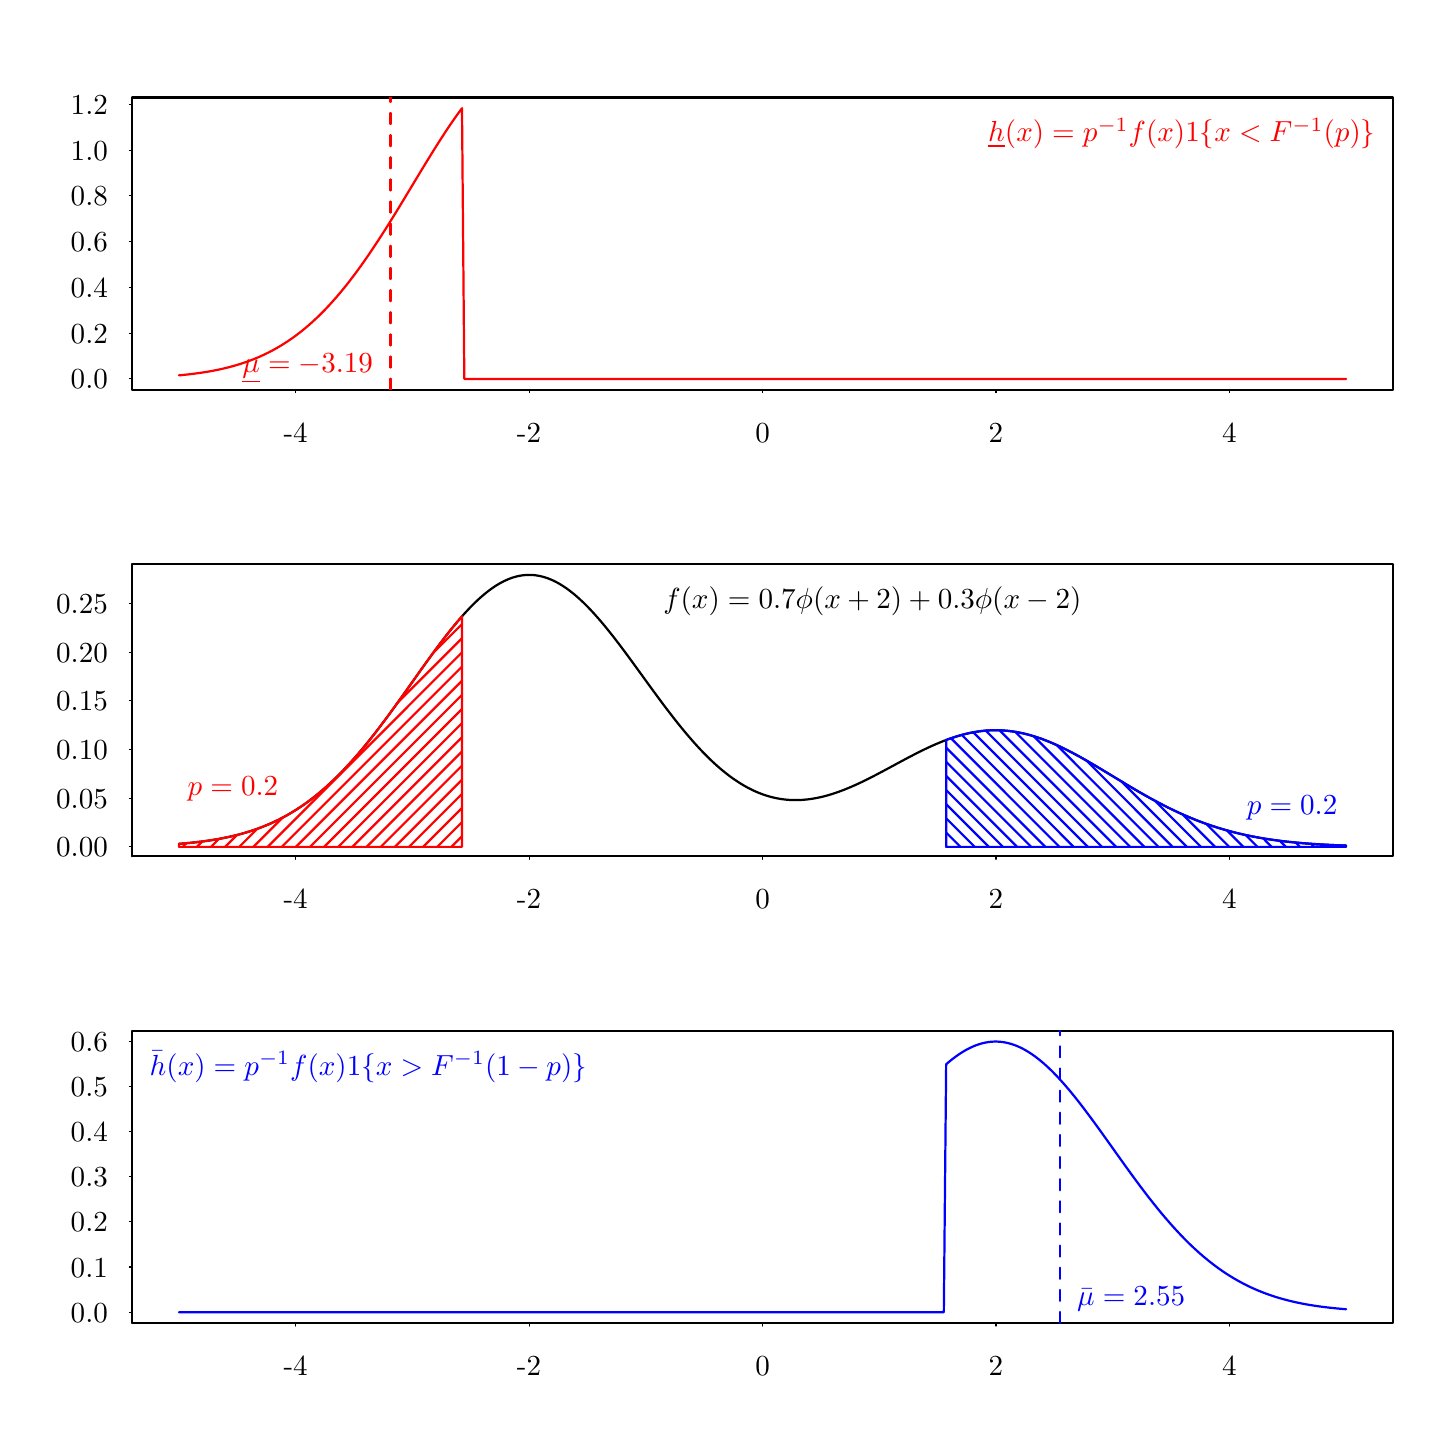
\begin{tikzpicture}[x=1pt,y=1pt]
\definecolor{fillColor}{RGB}{255,255,255}
\path[use as bounding box,fill=fillColor,fill opacity=0.00] (0,0) rectangle (505.89,505.89);
\begin{scope}
\path[clip] ( 37.80,375.06) rectangle (493.29,480.69);
\definecolor{drawColor}{RGB}{255,0,0}

\path[draw=drawColor,line width= 0.8pt,line join=round,line cap=round] ( 54.67,380.25) --
	( 55.52,380.33) --
	( 56.36,380.42) --
	( 57.21,380.50) --
	( 58.05,380.60) --
	( 58.90,380.70) --
	( 59.74,380.80) --
	( 60.59,380.91) --
	( 61.43,381.02) --
	( 62.28,381.14) --
	( 63.12,381.26) --
	( 63.97,381.40) --
	( 64.81,381.53) --
	( 65.66,381.68) --
	( 66.50,381.83) --
	( 67.35,381.99) --
	( 68.19,382.16) --
	( 69.04,382.33) --
	( 69.88,382.52) --
	( 70.73,382.71) --
	( 71.57,382.91) --
	( 72.42,383.12) --
	( 73.26,383.34) --
	( 74.11,383.57) --
	( 74.95,383.81) --
	( 75.80,384.06) --
	( 76.64,384.32) --
	( 77.49,384.59) --
	( 78.34,384.87) --
	( 79.18,385.16) --
	( 80.03,385.47) --
	( 80.87,385.79) --
	( 81.72,386.12) --
	( 82.56,386.46) --
	( 83.41,386.82) --
	( 84.25,387.19) --
	( 85.10,387.58) --
	( 85.94,387.98) --
	( 86.79,388.39) --
	( 87.63,388.82) --
	( 88.48,389.27) --
	( 89.32,389.73) --
	( 90.17,390.21) --
	( 91.01,390.70) --
	( 91.86,391.21) --
	( 92.70,391.74) --
	( 93.55,392.29) --
	( 94.39,392.85) --
	( 95.24,393.43) --
	( 96.08,394.03) --
	( 96.93,394.65) --
	( 97.77,395.29) --
	( 98.62,395.95) --
	( 99.47,396.62) --
	(100.31,397.32) --
	(101.16,398.03) --
	(102.00,398.77) --
	(102.85,399.52) --
	(103.69,400.30) --
	(104.54,401.09) --
	(105.38,401.91) --
	(106.23,402.74) --
	(107.07,403.60) --
	(107.92,404.48) --
	(108.76,405.38) --
	(109.61,406.30) --
	(110.45,407.24) --
	(111.30,408.20) --
	(112.14,409.18) --
	(112.99,410.18) --
	(113.83,411.20) --
	(114.68,412.24) --
	(115.52,413.30) --
	(116.37,414.38) --
	(117.21,415.49) --
	(118.06,416.60) --
	(118.90,417.74) --
	(119.75,418.90) --
	(120.59,420.07) --
	(121.44,421.27) --
	(122.29,422.48) --
	(123.13,423.70) --
	(123.98,424.94) --
	(124.82,426.20) --
	(125.67,427.47) --
	(126.51,428.76) --
	(127.36,430.06) --
	(128.20,431.37) --
	(129.05,432.70) --
	(129.89,434.04) --
	(130.74,435.38) --
	(131.58,436.74) --
	(132.43,438.11) --
	(133.27,439.48) --
	(134.12,440.86) --
	(134.96,442.25) --
	(135.81,443.64) --
	(136.65,445.04) --
	(137.50,446.44) --
	(138.34,447.84) --
	(139.19,449.24) --
	(140.03,450.65) --
	(140.88,452.05) --
	(141.72,453.45) --
	(142.57,454.84) --
	(143.41,456.23) --
	(144.26,457.61) --
	(145.11,458.99) --
	(145.95,460.36) --
	(146.80,461.72) --
	(147.64,463.06) --
	(148.49,464.40) --
	(149.33,465.72) --
	(150.18,467.02) --
	(151.02,468.31) --
	(151.87,469.58) --
	(152.71,470.84) --
	(153.56,472.07) --
	(154.40,473.28) --
	(155.25,474.47) --
	(156.09,475.64) --
	(156.94,476.78) --
	(157.78,378.97) --
	(158.63,378.97) --
	(159.47,378.97) --
	(160.32,378.97) --
	(161.16,378.97) --
	(162.01,378.97) --
	(162.85,378.97) --
	(163.70,378.97) --
	(164.54,378.97) --
	(165.39,378.97) --
	(166.24,378.97) --
	(167.08,378.97) --
	(167.93,378.97) --
	(168.77,378.97) --
	(169.62,378.97) --
	(170.46,378.97) --
	(171.31,378.97) --
	(172.15,378.97) --
	(173.00,378.97) --
	(173.84,378.97) --
	(174.69,378.97) --
	(175.53,378.97) --
	(176.38,378.97) --
	(177.22,378.97) --
	(178.07,378.97) --
	(178.91,378.97) --
	(179.76,378.97) --
	(180.60,378.97) --
	(181.45,378.97) --
	(182.29,378.97) --
	(183.14,378.97) --
	(183.98,378.97) --
	(184.83,378.97) --
	(185.67,378.97) --
	(186.52,378.97) --
	(187.36,378.97) --
	(188.21,378.97) --
	(189.06,378.97) --
	(189.90,378.97) --
	(190.75,378.97) --
	(191.59,378.97) --
	(192.44,378.97) --
	(193.28,378.97) --
	(194.13,378.97) --
	(194.97,378.97) --
	(195.82,378.97) --
	(196.66,378.97) --
	(197.51,378.97) --
	(198.35,378.97) --
	(199.20,378.97) --
	(200.04,378.97) --
	(200.89,378.97) --
	(201.73,378.97) --
	(202.58,378.97) --
	(203.42,378.97) --
	(204.27,378.97) --
	(205.11,378.97) --
	(205.96,378.97) --
	(206.80,378.97) --
	(207.65,378.97) --
	(208.49,378.97) --
	(209.34,378.97) --
	(210.19,378.97) --
	(211.03,378.97) --
	(211.88,378.97) --
	(212.72,378.97) --
	(213.57,378.97) --
	(214.41,378.97) --
	(215.26,378.97) --
	(216.10,378.97) --
	(216.95,378.97) --
	(217.79,378.97) --
	(218.64,378.97) --
	(219.48,378.97) --
	(220.33,378.97) --
	(221.17,378.97) --
	(222.02,378.97) --
	(222.86,378.97) --
	(223.71,378.97) --
	(224.55,378.97) --
	(225.40,378.97) --
	(226.24,378.97) --
	(227.09,378.97) --
	(227.93,378.97) --
	(228.78,378.97) --
	(229.62,378.97) --
	(230.47,378.97) --
	(231.31,378.97) --
	(232.16,378.97) --
	(233.01,378.97) --
	(233.85,378.97) --
	(234.70,378.97) --
	(235.54,378.97) --
	(236.39,378.97) --
	(237.23,378.97) --
	(238.08,378.97) --
	(238.92,378.97) --
	(239.77,378.97) --
	(240.61,378.97) --
	(241.46,378.97) --
	(242.30,378.97) --
	(243.15,378.97) --
	(243.99,378.97) --
	(244.84,378.97) --
	(245.68,378.97) --
	(246.53,378.97) --
	(247.37,378.97) --
	(248.22,378.97) --
	(249.06,378.97) --
	(249.91,378.97) --
	(250.75,378.97) --
	(251.60,378.97) --
	(252.44,378.97) --
	(253.29,378.97) --
	(254.13,378.97) --
	(254.98,378.97) --
	(255.83,378.97) --
	(256.67,378.97) --
	(257.52,378.97) --
	(258.36,378.97) --
	(259.21,378.97) --
	(260.05,378.97) --
	(260.90,378.97) --
	(261.74,378.97) --
	(262.59,378.97) --
	(263.43,378.97) --
	(264.28,378.97) --
	(265.12,378.97) --
	(265.97,378.97) --
	(266.81,378.97) --
	(267.66,378.97) --
	(268.50,378.97) --
	(269.35,378.97) --
	(270.19,378.97) --
	(271.04,378.97) --
	(271.88,378.97) --
	(272.73,378.97) --
	(273.57,378.97) --
	(274.42,378.97) --
	(275.26,378.97) --
	(276.11,378.97) --
	(276.96,378.97) --
	(277.80,378.97) --
	(278.65,378.97) --
	(279.49,378.97) --
	(280.34,378.97) --
	(281.18,378.97) --
	(282.03,378.97) --
	(282.87,378.97) --
	(283.72,378.97) --
	(284.56,378.97) --
	(285.41,378.97) --
	(286.25,378.97) --
	(287.10,378.97) --
	(287.94,378.97) --
	(288.79,378.97) --
	(289.63,378.97) --
	(290.48,378.97) --
	(291.32,378.97) --
	(292.17,378.97) --
	(293.01,378.97) --
	(293.86,378.97) --
	(294.70,378.97) --
	(295.55,378.97) --
	(296.39,378.97) --
	(297.24,378.97) --
	(298.08,378.97) --
	(298.93,378.97) --
	(299.78,378.97) --
	(300.62,378.97) --
	(301.47,378.97) --
	(302.31,378.97) --
	(303.16,378.97) --
	(304.00,378.97) --
	(304.85,378.97) --
	(305.69,378.97) --
	(306.54,378.97) --
	(307.38,378.97) --
	(308.23,378.97) --
	(309.07,378.97) --
	(309.92,378.97) --
	(310.76,378.97) --
	(311.61,378.97) --
	(312.45,378.97) --
	(313.30,378.97) --
	(314.14,378.97) --
	(314.99,378.97) --
	(315.83,378.97) --
	(316.68,378.97) --
	(317.52,378.97) --
	(318.37,378.97) --
	(319.21,378.97) --
	(320.06,378.97) --
	(320.90,378.97) --
	(321.75,378.97) --
	(322.60,378.97) --
	(323.44,378.97) --
	(324.29,378.97) --
	(325.13,378.97) --
	(325.98,378.97) --
	(326.82,378.97) --
	(327.67,378.97) --
	(328.51,378.97) --
	(329.36,378.97) --
	(330.20,378.97) --
	(331.05,378.97) --
	(331.89,378.97) --
	(332.74,378.97) --
	(333.58,378.97) --
	(334.43,378.97) --
	(335.27,378.97) --
	(336.12,378.97) --
	(336.96,378.97) --
	(337.81,378.97) --
	(338.65,378.97) --
	(339.50,378.97) --
	(340.34,378.97) --
	(341.19,378.97) --
	(342.03,378.97) --
	(342.88,378.97) --
	(343.73,378.97) --
	(344.57,378.97) --
	(345.42,378.97) --
	(346.26,378.97) --
	(347.11,378.97) --
	(347.95,378.97) --
	(348.80,378.97) --
	(349.64,378.97) --
	(350.49,378.97) --
	(351.33,378.97) --
	(352.18,378.97) --
	(353.02,378.97) --
	(353.87,378.97) --
	(354.71,378.97) --
	(355.56,378.97) --
	(356.40,378.97) --
	(357.25,378.97) --
	(358.09,378.97) --
	(358.94,378.97) --
	(359.78,378.97) --
	(360.63,378.97) --
	(361.47,378.97) --
	(362.32,378.97) --
	(363.16,378.97) --
	(364.01,378.97) --
	(364.85,378.97) --
	(365.70,378.97) --
	(366.55,378.97) --
	(367.39,378.97) --
	(368.24,378.97) --
	(369.08,378.97) --
	(369.93,378.97) --
	(370.77,378.97) --
	(371.62,378.97) --
	(372.46,378.97) --
	(373.31,378.97) --
	(374.15,378.97) --
	(375.00,378.97) --
	(375.84,378.97) --
	(376.69,378.97) --
	(377.53,378.97) --
	(378.38,378.97) --
	(379.22,378.97) --
	(380.07,378.97) --
	(380.91,378.97) --
	(381.76,378.97) --
	(382.60,378.97) --
	(383.45,378.97) --
	(384.29,378.97) --
	(385.14,378.97) --
	(385.98,378.97) --
	(386.83,378.97) --
	(387.68,378.97) --
	(388.52,378.97) --
	(389.37,378.97) --
	(390.21,378.97) --
	(391.06,378.97) --
	(391.90,378.97) --
	(392.75,378.97) --
	(393.59,378.97) --
	(394.44,378.97) --
	(395.28,378.97) --
	(396.13,378.97) --
	(396.97,378.97) --
	(397.82,378.97) --
	(398.66,378.97) --
	(399.51,378.97) --
	(400.35,378.97) --
	(401.20,378.97) --
	(402.04,378.97) --
	(402.89,378.97) --
	(403.73,378.97) --
	(404.58,378.97) --
	(405.42,378.97) --
	(406.27,378.97) --
	(407.11,378.97) --
	(407.96,378.97) --
	(408.80,378.97) --
	(409.65,378.97) --
	(410.50,378.97) --
	(411.34,378.97) --
	(412.19,378.97) --
	(413.03,378.97) --
	(413.88,378.97) --
	(414.72,378.97) --
	(415.57,378.97) --
	(416.41,378.97) --
	(417.26,378.97) --
	(418.10,378.97) --
	(418.95,378.97) --
	(419.79,378.97) --
	(420.64,378.97) --
	(421.48,378.97) --
	(422.33,378.97) --
	(423.17,378.97) --
	(424.02,378.97) --
	(424.86,378.97) --
	(425.71,378.97) --
	(426.55,378.97) --
	(427.40,378.97) --
	(428.24,378.97) --
	(429.09,378.97) --
	(429.93,378.97) --
	(430.78,378.97) --
	(431.62,378.97) --
	(432.47,378.97) --
	(433.32,378.97) --
	(434.16,378.97) --
	(435.01,378.97) --
	(435.85,378.97) --
	(436.70,378.97) --
	(437.54,378.97) --
	(438.39,378.97) --
	(439.23,378.97) --
	(440.08,378.97) --
	(440.92,378.97) --
	(441.77,378.97) --
	(442.61,378.97) --
	(443.46,378.97) --
	(444.30,378.97) --
	(445.15,378.97) --
	(445.99,378.97) --
	(446.84,378.97) --
	(447.68,378.97) --
	(448.53,378.97) --
	(449.37,378.97) --
	(450.22,378.97) --
	(451.06,378.97) --
	(451.91,378.97) --
	(452.75,378.97) --
	(453.60,378.97) --
	(454.45,378.97) --
	(455.29,378.97) --
	(456.14,378.97) --
	(456.98,378.97) --
	(457.83,378.97) --
	(458.67,378.97) --
	(459.52,378.97) --
	(460.36,378.97) --
	(461.21,378.97) --
	(462.05,378.97) --
	(462.90,378.97) --
	(463.74,378.97) --
	(464.59,378.97) --
	(465.43,378.97) --
	(466.28,378.97) --
	(467.12,378.97) --
	(467.97,378.97) --
	(468.81,378.97) --
	(469.66,378.97) --
	(470.50,378.97) --
	(471.35,378.97) --
	(472.19,378.97) --
	(473.04,378.97) --
	(473.88,378.97) --
	(474.73,378.97) --
	(475.57,378.97) --
	(476.42,378.97);
\end{scope}
\begin{scope}
\path[clip] (  0.00,  0.00) rectangle (505.89,505.89);
\definecolor{drawColor}{RGB}{0,0,0}

\path[draw=drawColor,line width= 0.4pt,line join=round,line cap=round] ( 96.84,375.06) -- (434.25,375.06);

\path[draw=drawColor,line width= 0.4pt,line join=round,line cap=round] ( 96.84,375.06) -- ( 96.84,374.00);

\path[draw=drawColor,line width= 0.4pt,line join=round,line cap=round] (181.19,375.06) -- (181.19,374.00);

\path[draw=drawColor,line width= 0.4pt,line join=round,line cap=round] (265.54,375.06) -- (265.54,374.00);

\path[draw=drawColor,line width= 0.4pt,line join=round,line cap=round] (349.89,375.06) -- (349.89,374.00);

\path[draw=drawColor,line width= 0.4pt,line join=round,line cap=round] (434.25,375.06) -- (434.25,374.00);

\node[text=drawColor,anchor=base,inner sep=0pt, outer sep=0pt, scale=  1.05] at ( 96.84,356.16) {-4};

\node[text=drawColor,anchor=base,inner sep=0pt, outer sep=0pt, scale=  1.05] at (181.19,356.16) {-2};

\node[text=drawColor,anchor=base,inner sep=0pt, outer sep=0pt, scale=  1.05] at (265.54,356.16) {0};

\node[text=drawColor,anchor=base,inner sep=0pt, outer sep=0pt, scale=  1.05] at (349.89,356.16) {2};

\node[text=drawColor,anchor=base,inner sep=0pt, outer sep=0pt, scale=  1.05] at (434.25,356.16) {4};

\path[draw=drawColor,line width= 0.4pt,line join=round,line cap=round] ( 37.80,378.97) -- ( 37.80,478.14);

\path[draw=drawColor,line width= 0.4pt,line join=round,line cap=round] ( 37.80,378.97) -- ( 36.74,378.97);

\path[draw=drawColor,line width= 0.4pt,line join=round,line cap=round] ( 37.80,395.50) -- ( 36.74,395.50);

\path[draw=drawColor,line width= 0.4pt,line join=round,line cap=round] ( 37.80,412.03) -- ( 36.74,412.03);

\path[draw=drawColor,line width= 0.4pt,line join=round,line cap=round] ( 37.80,428.56) -- ( 36.74,428.56);

\path[draw=drawColor,line width= 0.4pt,line join=round,line cap=round] ( 37.80,445.09) -- ( 36.74,445.09);

\path[draw=drawColor,line width= 0.4pt,line join=round,line cap=round] ( 37.80,461.62) -- ( 36.74,461.62);

\path[draw=drawColor,line width= 0.4pt,line join=round,line cap=round] ( 37.80,478.14) -- ( 36.74,478.14);

\node[text=drawColor,anchor=base east,inner sep=0pt, outer sep=0pt, scale=  1.05] at ( 28.98,375.36) {0.0};

\node[text=drawColor,anchor=base east,inner sep=0pt, outer sep=0pt, scale=  1.05] at ( 28.98,391.89) {0.2};

\node[text=drawColor,anchor=base east,inner sep=0pt, outer sep=0pt, scale=  1.05] at ( 28.98,408.41) {0.4};

\node[text=drawColor,anchor=base east,inner sep=0pt, outer sep=0pt, scale=  1.05] at ( 28.98,424.94) {0.6};

\node[text=drawColor,anchor=base east,inner sep=0pt, outer sep=0pt, scale=  1.05] at ( 28.98,441.47) {0.8};

\node[text=drawColor,anchor=base east,inner sep=0pt, outer sep=0pt, scale=  1.05] at ( 28.98,458.00) {1.0};

\node[text=drawColor,anchor=base east,inner sep=0pt, outer sep=0pt, scale=  1.05] at ( 28.98,474.53) {1.2};

\path[draw=drawColor,line width= 0.8pt,line join=round,line cap=round] ( 37.80,375.06) --
	(493.29,375.06) --
	(493.29,480.69) --
	( 37.80,480.69) --
	( 37.80,375.06);
\end{scope}
\begin{scope}
\path[clip] ( 37.80,375.06) rectangle (493.29,480.69);
\definecolor{drawColor}{RGB}{255,0,0}

\node[text=drawColor,anchor=base east,inner sep=0pt, outer sep=0pt, scale=  1.05] at (486.99,464.59) {$\underline{h}(x) = p^{-1}f(x) 1\{x < F^{-1}(p)\}$};

\path[draw=drawColor,line width= 0.8pt,dash pattern=on 4pt off 4pt ,line join=round,line cap=round] (131.07,375.06) -- (131.07,480.69);

\node[text=drawColor,anchor=base east,inner sep=0pt, outer sep=0pt, scale=  1.05] at (124.77,381.45) {$\underline{\mu} = -3.19$};
\end{scope}
\begin{scope}
\path[clip] ( 37.80,206.43) rectangle (493.29,312.06);
\definecolor{drawColor}{RGB}{0,0,0}

\path[draw=drawColor,line width= 0.8pt,line join=round,line cap=round] ( 54.67,210.97) --
	( 55.52,211.03) --
	( 56.36,211.10) --
	( 57.21,211.18) --
	( 58.05,211.26) --
	( 58.90,211.34) --
	( 59.74,211.43) --
	( 60.59,211.52) --
	( 61.43,211.62) --
	( 62.28,211.72) --
	( 63.12,211.83) --
	( 63.97,211.94) --
	( 64.81,212.06) --
	( 65.66,212.18) --
	( 66.50,212.31) --
	( 67.35,212.45) --
	( 68.19,212.59) --
	( 69.04,212.74) --
	( 69.88,212.89) --
	( 70.73,213.06) --
	( 71.57,213.23) --
	( 72.42,213.41) --
	( 73.26,213.59) --
	( 74.11,213.79) --
	( 74.95,213.99) --
	( 75.80,214.20) --
	( 76.64,214.42) --
	( 77.49,214.65) --
	( 78.34,214.90) --
	( 79.18,215.15) --
	( 80.03,215.41) --
	( 80.87,215.68) --
	( 81.72,215.96) --
	( 82.56,216.25) --
	( 83.41,216.56) --
	( 84.25,216.87) --
	( 85.10,217.20) --
	( 85.94,217.54) --
	( 86.79,217.90) --
	( 87.63,218.26) --
	( 88.48,218.64) --
	( 89.32,219.04) --
	( 90.17,219.44) --
	( 91.01,219.86) --
	( 91.86,220.30) --
	( 92.70,220.75) --
	( 93.55,221.21) --
	( 94.39,221.69) --
	( 95.24,222.19) --
	( 96.08,222.70) --
	( 96.93,223.23) --
	( 97.77,223.77) --
	( 98.62,224.33) --
	( 99.47,224.90) --
	(100.31,225.49) --
	(101.16,226.10) --
	(102.00,226.73) --
	(102.85,227.37) --
	(103.69,228.03) --
	(104.54,228.71) --
	(105.38,229.40) --
	(106.23,230.12) --
	(107.07,230.85) --
	(107.92,231.59) --
	(108.76,232.36) --
	(109.61,233.14) --
	(110.45,233.94) --
	(111.30,234.76) --
	(112.14,235.59) --
	(112.99,236.45) --
	(113.83,237.32) --
	(114.68,238.20) --
	(115.52,239.11) --
	(116.37,240.03) --
	(117.21,240.97) --
	(118.06,241.92) --
	(118.90,242.89) --
	(119.75,243.87) --
	(120.59,244.87) --
	(121.44,245.89) --
	(122.29,246.92) --
	(123.13,247.96) --
	(123.98,249.02) --
	(124.82,250.09) --
	(125.67,251.17) --
	(126.51,252.27) --
	(127.36,253.38) --
	(128.20,254.50) --
	(129.05,255.62) --
	(129.89,256.76) --
	(130.74,257.91) --
	(131.58,259.07) --
	(132.43,260.23) --
	(133.27,261.40) --
	(134.12,262.58) --
	(134.96,263.76) --
	(135.81,264.94) --
	(136.65,266.13) --
	(137.50,267.32) --
	(138.34,268.52) --
	(139.19,269.71) --
	(140.03,270.91) --
	(140.88,272.10) --
	(141.72,273.29) --
	(142.57,274.48) --
	(143.41,275.66) --
	(144.26,276.84) --
	(145.11,278.01) --
	(145.95,279.18) --
	(146.80,280.33) --
	(147.64,281.48) --
	(148.49,282.61) --
	(149.33,283.74) --
	(150.18,284.85) --
	(151.02,285.95) --
	(151.87,287.03) --
	(152.71,288.10) --
	(153.56,289.15) --
	(154.40,290.18) --
	(155.25,291.19) --
	(156.09,292.19) --
	(156.94,293.16) --
	(157.78,294.11) --
	(158.63,295.03) --
	(159.47,295.93) --
	(160.32,296.81) --
	(161.16,297.66) --
	(162.01,298.48) --
	(162.85,299.27) --
	(163.70,300.04) --
	(164.54,300.77) --
	(165.39,301.47) --
	(166.24,302.15) --
	(167.08,302.79) --
	(167.93,303.39) --
	(168.77,303.97) --
	(169.62,304.51) --
	(170.46,305.01) --
	(171.31,305.48) --
	(172.15,305.91) --
	(173.00,306.30) --
	(173.84,306.66) --
	(174.69,306.98) --
	(175.53,307.26) --
	(176.38,307.50) --
	(177.22,307.71) --
	(178.07,307.88) --
	(178.91,308.00) --
	(179.76,308.09) --
	(180.60,308.14) --
	(181.45,308.15) --
	(182.29,308.12) --
	(183.14,308.05) --
	(183.98,307.94) --
	(184.83,307.79) --
	(185.67,307.60) --
	(186.52,307.38) --
	(187.36,307.11) --
	(188.21,306.81) --
	(189.06,306.47) --
	(189.90,306.10) --
	(190.75,305.68) --
	(191.59,305.23) --
	(192.44,304.75) --
	(193.28,304.22) --
	(194.13,303.67) --
	(194.97,303.08) --
	(195.82,302.46) --
	(196.66,301.80) --
	(197.51,301.12) --
	(198.35,300.40) --
	(199.20,299.65) --
	(200.04,298.87) --
	(200.89,298.07) --
	(201.73,297.24) --
	(202.58,296.38) --
	(203.42,295.49) --
	(204.27,294.59) --
	(205.11,293.65) --
	(205.96,292.70) --
	(206.80,291.73) --
	(207.65,290.73) --
	(208.49,289.72) --
	(209.34,288.68) --
	(210.19,287.63) --
	(211.03,286.57) --
	(211.88,285.49) --
	(212.72,284.40) --
	(213.57,283.29) --
	(214.41,282.18) --
	(215.26,281.05) --
	(216.10,279.91) --
	(216.95,278.77) --
	(217.79,277.62) --
	(218.64,276.46) --
	(219.48,275.30) --
	(220.33,274.14) --
	(221.17,272.97) --
	(222.02,271.81) --
	(222.86,270.64) --
	(223.71,269.47) --
	(224.55,268.31) --
	(225.40,267.15) --
	(226.24,265.99) --
	(227.09,264.84) --
	(227.93,263.69) --
	(228.78,262.55) --
	(229.62,261.42) --
	(230.47,260.29) --
	(231.31,259.18) --
	(232.16,258.08) --
	(233.01,256.98) --
	(233.85,255.90) --
	(234.70,254.83) --
	(235.54,253.78) --
	(236.39,252.74) --
	(237.23,251.71) --
	(238.08,250.70) --
	(238.92,249.71) --
	(239.77,248.73) --
	(240.61,247.77) --
	(241.46,246.82) --
	(242.30,245.90) --
	(243.15,244.99) --
	(243.99,244.10) --
	(244.84,243.24) --
	(245.68,242.39) --
	(246.53,241.56) --
	(247.37,240.76) --
	(248.22,239.97) --
	(249.06,239.21) --
	(249.91,238.47) --
	(250.75,237.75) --
	(251.60,237.05) --
	(252.44,236.38) --
	(253.29,235.73) --
	(254.13,235.10) --
	(254.98,234.49) --
	(255.83,233.91) --
	(256.67,233.35) --
	(257.52,232.81) --
	(258.36,232.30) --
	(259.21,231.81) --
	(260.05,231.34) --
	(260.90,230.90) --
	(261.74,230.48) --
	(262.59,230.08) --
	(263.43,229.70) --
	(264.28,229.35) --
	(265.12,229.03) --
	(265.97,228.72) --
	(266.81,228.44) --
	(267.66,228.18) --
	(268.50,227.94) --
	(269.35,227.73) --
	(270.19,227.54) --
	(271.04,227.37) --
	(271.88,227.22) --
	(272.73,227.09) --
	(273.57,226.99) --
	(274.42,226.90) --
	(275.26,226.84) --
	(276.11,226.80) --
	(276.96,226.78) --
	(277.80,226.77) --
	(278.65,226.79) --
	(279.49,226.83) --
	(280.34,226.88) --
	(281.18,226.96) --
	(282.03,227.05) --
	(282.87,227.16) --
	(283.72,227.29) --
	(284.56,227.44) --
	(285.41,227.60) --
	(286.25,227.78) --
	(287.10,227.97) --
	(287.94,228.18) --
	(288.79,228.41) --
	(289.63,228.65) --
	(290.48,228.91) --
	(291.32,229.18) --
	(292.17,229.46) --
	(293.01,229.76) --
	(293.86,230.07) --
	(294.70,230.39) --
	(295.55,230.72) --
	(296.39,231.07) --
	(297.24,231.42) --
	(298.08,231.79) --
	(298.93,232.16) --
	(299.78,232.55) --
	(300.62,232.94) --
	(301.47,233.34) --
	(302.31,233.75) --
	(303.16,234.16) --
	(304.00,234.59) --
	(304.85,235.01) --
	(305.69,235.45) --
	(306.54,235.89) --
	(307.38,236.33) --
	(308.23,236.78) --
	(309.07,237.23) --
	(309.92,237.68) --
	(310.76,238.13) --
	(311.61,238.59) --
	(312.45,239.05) --
	(313.30,239.50) --
	(314.14,239.96) --
	(314.99,240.41) --
	(315.83,240.87) --
	(316.68,241.32) --
	(317.52,241.77) --
	(318.37,242.22) --
	(319.21,242.66) --
	(320.06,243.10) --
	(320.90,243.53) --
	(321.75,243.96) --
	(322.60,244.38) --
	(323.44,244.80) --
	(324.29,245.21) --
	(325.13,245.61) --
	(325.98,246.00) --
	(326.82,246.39) --
	(327.67,246.76) --
	(328.51,247.13) --
	(329.36,247.48) --
	(330.20,247.83) --
	(331.05,248.16) --
	(331.89,248.49) --
	(332.74,248.80) --
	(333.58,249.09) --
	(334.43,249.38) --
	(335.27,249.65) --
	(336.12,249.91) --
	(336.96,250.16) --
	(337.81,250.39) --
	(338.65,250.61) --
	(339.50,250.81) --
	(340.34,251.00) --
	(341.19,251.17) --
	(342.03,251.33) --
	(342.88,251.47) --
	(343.73,251.60) --
	(344.57,251.71) --
	(345.42,251.80) --
	(346.26,251.88) --
	(347.11,251.94) --
	(347.95,251.98) --
	(348.80,252.01) --
	(349.64,252.02) --
	(350.49,252.01) --
	(351.33,251.99) --
	(352.18,251.95) --
	(353.02,251.89) --
	(353.87,251.82) --
	(354.71,251.73) --
	(355.56,251.63) --
	(356.40,251.51) --
	(357.25,251.37) --
	(358.09,251.21) --
	(358.94,251.04) --
	(359.78,250.86) --
	(360.63,250.66) --
	(361.47,250.44) --
	(362.32,250.21) --
	(363.16,249.96) --
	(364.01,249.70) --
	(364.85,249.43) --
	(365.70,249.14) --
	(366.55,248.84) --
	(367.39,248.52) --
	(368.24,248.19) --
	(369.08,247.85) --
	(369.93,247.50) --
	(370.77,247.13) --
	(371.62,246.76) --
	(372.46,246.37) --
	(373.31,245.98) --
	(374.15,245.57) --
	(375.00,245.15) --
	(375.84,244.73) --
	(376.69,244.29) --
	(377.53,243.85) --
	(378.38,243.40) --
	(379.22,242.94) --
	(380.07,242.48) --
	(380.91,242.01) --
	(381.76,241.53) --
	(382.60,241.05) --
	(383.45,240.56) --
	(384.29,240.07) --
	(385.14,239.58) --
	(385.98,239.08) --
	(386.83,238.57) --
	(387.68,238.07) --
	(388.52,237.56) --
	(389.37,237.05) --
	(390.21,236.54) --
	(391.06,236.03) --
	(391.90,235.52) --
	(392.75,235.01) --
	(393.59,234.50) --
	(394.44,233.98) --
	(395.28,233.48) --
	(396.13,232.97) --
	(396.97,232.46) --
	(397.82,231.96) --
	(398.66,231.46) --
	(399.51,230.96) --
	(400.35,230.46) --
	(401.20,229.97) --
	(402.04,229.48) --
	(402.89,229.00) --
	(403.73,228.52) --
	(404.58,228.04) --
	(405.42,227.57) --
	(406.27,227.11) --
	(407.11,226.65) --
	(407.96,226.20) --
	(408.80,225.75) --
	(409.65,225.31) --
	(410.50,224.87) --
	(411.34,224.45) --
	(412.19,224.02) --
	(413.03,223.61) --
	(413.88,223.20) --
	(414.72,222.80) --
	(415.57,222.40) --
	(416.41,222.02) --
	(417.26,221.64) --
	(418.10,221.26) --
	(418.95,220.90) --
	(419.79,220.54) --
	(420.64,220.19) --
	(421.48,219.85) --
	(422.33,219.51) --
	(423.17,219.18) --
	(424.02,218.86) --
	(424.86,218.55) --
	(425.71,218.24) --
	(426.55,217.95) --
	(427.40,217.66) --
	(428.24,217.37) --
	(429.09,217.10) --
	(429.93,216.83) --
	(430.78,216.57) --
	(431.62,216.32) --
	(432.47,216.07) --
	(433.32,215.83) --
	(434.16,215.60) --
	(435.01,215.37) --
	(435.85,215.15) --
	(436.70,214.94) --
	(437.54,214.73) --
	(438.39,214.53) --
	(439.23,214.34) --
	(440.08,214.16) --
	(440.92,213.98) --
	(441.77,213.80) --
	(442.61,213.63) --
	(443.46,213.47) --
	(444.30,213.31) --
	(445.15,213.16) --
	(445.99,213.02) --
	(446.84,212.87) --
	(447.68,212.74) --
	(448.53,212.61) --
	(449.37,212.48) --
	(450.22,212.36) --
	(451.06,212.25) --
	(451.91,212.13) --
	(452.75,212.03) --
	(453.60,211.92) --
	(454.45,211.82) --
	(455.29,211.73) --
	(456.14,211.64) --
	(456.98,211.55) --
	(457.83,211.47) --
	(458.67,211.39) --
	(459.52,211.31) --
	(460.36,211.24) --
	(461.21,211.17) --
	(462.05,211.10) --
	(462.90,211.04) --
	(463.74,210.98) --
	(464.59,210.92) --
	(465.43,210.86) --
	(466.28,210.81) --
	(467.12,210.76) --
	(467.97,210.71) --
	(468.81,210.67) --
	(469.66,210.62) --
	(470.50,210.58) --
	(471.35,210.54) --
	(472.19,210.50) --
	(473.04,210.47) --
	(473.88,210.43) --
	(474.73,210.40) --
	(475.57,210.37) --
	(476.42,210.34);
\end{scope}
\begin{scope}
\path[clip] (  0.00,  0.00) rectangle (505.89,505.89);
\definecolor{drawColor}{RGB}{0,0,0}

\path[draw=drawColor,line width= 0.4pt,line join=round,line cap=round] ( 96.84,206.43) -- (434.25,206.43);

\path[draw=drawColor,line width= 0.4pt,line join=round,line cap=round] ( 96.84,206.43) -- ( 96.84,205.37);

\path[draw=drawColor,line width= 0.4pt,line join=round,line cap=round] (181.19,206.43) -- (181.19,205.37);

\path[draw=drawColor,line width= 0.4pt,line join=round,line cap=round] (265.54,206.43) -- (265.54,205.37);

\path[draw=drawColor,line width= 0.4pt,line join=round,line cap=round] (349.89,206.43) -- (349.89,205.37);

\path[draw=drawColor,line width= 0.4pt,line join=round,line cap=round] (434.25,206.43) -- (434.25,205.37);

\node[text=drawColor,anchor=base,inner sep=0pt, outer sep=0pt, scale=  1.05] at ( 96.84,187.53) {-4};

\node[text=drawColor,anchor=base,inner sep=0pt, outer sep=0pt, scale=  1.05] at (181.19,187.53) {-2};

\node[text=drawColor,anchor=base,inner sep=0pt, outer sep=0pt, scale=  1.05] at (265.54,187.53) {0};

\node[text=drawColor,anchor=base,inner sep=0pt, outer sep=0pt, scale=  1.05] at (349.89,187.53) {2};

\node[text=drawColor,anchor=base,inner sep=0pt, outer sep=0pt, scale=  1.05] at (434.25,187.53) {4};

\path[draw=drawColor,line width= 0.4pt,line join=round,line cap=round] ( 37.80,209.87) -- ( 37.80,297.84);

\path[draw=drawColor,line width= 0.4pt,line join=round,line cap=round] ( 37.80,209.87) -- ( 36.74,209.87);

\path[draw=drawColor,line width= 0.4pt,line join=round,line cap=round] ( 37.80,227.47) -- ( 36.74,227.47);

\path[draw=drawColor,line width= 0.4pt,line join=round,line cap=round] ( 37.80,245.06) -- ( 36.74,245.06);

\path[draw=drawColor,line width= 0.4pt,line join=round,line cap=round] ( 37.80,262.65) -- ( 36.74,262.65);

\path[draw=drawColor,line width= 0.4pt,line join=round,line cap=round] ( 37.80,280.25) -- ( 36.74,280.25);

\path[draw=drawColor,line width= 0.4pt,line join=round,line cap=round] ( 37.80,297.84) -- ( 36.74,297.84);

\node[text=drawColor,anchor=base east,inner sep=0pt, outer sep=0pt, scale=  1.05] at ( 28.98,206.26) {0.00};

\node[text=drawColor,anchor=base east,inner sep=0pt, outer sep=0pt, scale=  1.05] at ( 28.98,223.85) {0.05};

\node[text=drawColor,anchor=base east,inner sep=0pt, outer sep=0pt, scale=  1.05] at ( 28.98,241.44) {0.10};

\node[text=drawColor,anchor=base east,inner sep=0pt, outer sep=0pt, scale=  1.05] at ( 28.98,259.04) {0.15};

\node[text=drawColor,anchor=base east,inner sep=0pt, outer sep=0pt, scale=  1.05] at ( 28.98,276.63) {0.20};

\node[text=drawColor,anchor=base east,inner sep=0pt, outer sep=0pt, scale=  1.05] at ( 28.98,294.22) {0.25};

\path[draw=drawColor,line width= 0.8pt,line join=round,line cap=round] ( 37.80,206.43) --
	(493.29,206.43) --
	(493.29,312.06) --
	( 37.80,312.06) --
	( 37.80,206.43);
\end{scope}
\begin{scope}
\path[clip] ( 37.80,206.43) rectangle (493.29,312.06);
\definecolor{drawColor}{RGB}{255,0,0}

\path[draw=drawColor,line width= 0.8pt,line join=round,line cap=round] ( 56.02,209.87) -- ( 57.34,211.19);

\path[draw=drawColor,line width= 0.8pt,line join=round,line cap=round] ( 61.13,209.87) -- ( 63.08,211.82);

\path[draw=drawColor,line width= 0.8pt,line join=round,line cap=round] ( 66.24,209.87) -- ( 69.12,212.75);

\path[draw=drawColor,line width= 0.8pt,line join=round,line cap=round] ( 71.36,209.87) -- ( 75.64,214.16);

\path[draw=drawColor,line width= 0.8pt,line join=round,line cap=round] ( 76.47,209.87) -- ( 83.00,216.41);

\path[draw=drawColor,line width= 0.8pt,line join=round,line cap=round] (146.45,279.86) -- (156.94,290.35);

\path[draw=drawColor,line width= 0.8pt,line join=round,line cap=round] ( 81.58,209.87) -- ( 92.16,220.46);

\path[draw=drawColor,line width= 0.8pt,line join=round,line cap=round] (133.71,262.01) -- (156.94,285.24);

\path[draw=drawColor,line width= 0.8pt,line join=round,line cap=round] ( 86.69,209.87) -- (156.94,280.13);

\path[draw=drawColor,line width= 0.8pt,line join=round,line cap=round] ( 91.80,209.87) -- (156.94,275.02);

\path[draw=drawColor,line width= 0.8pt,line join=round,line cap=round] ( 96.91,209.87) -- (156.94,269.91);

\path[draw=drawColor,line width= 0.8pt,line join=round,line cap=round] (102.02,209.87) -- (156.94,264.80);

\path[draw=drawColor,line width= 0.8pt,line join=round,line cap=round] (107.13,209.87) -- (156.94,259.69);

\path[draw=drawColor,line width= 0.8pt,line join=round,line cap=round] (112.24,209.87) -- (156.94,254.58);

\path[draw=drawColor,line width= 0.8pt,line join=round,line cap=round] (117.35,209.87) -- (156.94,249.46);

\path[draw=drawColor,line width= 0.8pt,line join=round,line cap=round] (122.46,209.87) -- (156.94,244.35);

\path[draw=drawColor,line width= 0.8pt,line join=round,line cap=round] (127.57,209.87) -- (156.94,239.24);

\path[draw=drawColor,line width= 0.8pt,line join=round,line cap=round] (132.68,209.87) -- (156.94,234.13);

\path[draw=drawColor,line width= 0.8pt,line join=round,line cap=round] (137.79,209.87) -- (156.94,229.02);

\path[draw=drawColor,line width= 0.8pt,line join=round,line cap=round] (142.90,209.87) -- (156.94,223.91);

\path[draw=drawColor,line width= 0.8pt,line join=round,line cap=round] (148.01,209.87) -- (156.94,218.80);

\path[draw=drawColor,line width= 0.8pt,line join=round,line cap=round] (153.12,209.87) -- (156.94,213.69);

\path[draw=drawColor,line width= 0.8pt,line join=round,line cap=round] ( 54.67,209.87) --
	( 55.52,209.87) --
	( 56.36,209.87) --
	( 57.21,209.87) --
	( 58.05,209.87) --
	( 58.90,209.87) --
	( 59.74,209.87) --
	( 60.59,209.87) --
	( 61.43,209.87) --
	( 62.28,209.87) --
	( 63.12,209.87) --
	( 63.97,209.87) --
	( 64.81,209.87) --
	( 65.66,209.87) --
	( 66.50,209.87) --
	( 67.35,209.87) --
	( 68.19,209.87) --
	( 69.04,209.87) --
	( 69.88,209.87) --
	( 70.73,209.87) --
	( 71.57,209.87) --
	( 72.42,209.87) --
	( 73.26,209.87) --
	( 74.11,209.87) --
	( 74.95,209.87) --
	( 75.80,209.87) --
	( 76.64,209.87) --
	( 77.49,209.87) --
	( 78.34,209.87) --
	( 79.18,209.87) --
	( 80.03,209.87) --
	( 80.87,209.87) --
	( 81.72,209.87) --
	( 82.56,209.87) --
	( 83.41,209.87) --
	( 84.25,209.87) --
	( 85.10,209.87) --
	( 85.94,209.87) --
	( 86.79,209.87) --
	( 87.63,209.87) --
	( 88.48,209.87) --
	( 89.32,209.87) --
	( 90.17,209.87) --
	( 91.01,209.87) --
	( 91.86,209.87) --
	( 92.70,209.87) --
	( 93.55,209.87) --
	( 94.39,209.87) --
	( 95.24,209.87) --
	( 96.08,209.87) --
	( 96.93,209.87) --
	( 97.77,209.87) --
	( 98.62,209.87) --
	( 99.47,209.87) --
	(100.31,209.87) --
	(101.16,209.87) --
	(102.00,209.87) --
	(102.85,209.87) --
	(103.69,209.87) --
	(104.54,209.87) --
	(105.38,209.87) --
	(106.23,209.87) --
	(107.07,209.87) --
	(107.92,209.87) --
	(108.76,209.87) --
	(109.61,209.87) --
	(110.45,209.87) --
	(111.30,209.87) --
	(112.14,209.87) --
	(112.99,209.87) --
	(113.83,209.87) --
	(114.68,209.87) --
	(115.52,209.87) --
	(116.37,209.87) --
	(117.21,209.87) --
	(118.06,209.87) --
	(118.90,209.87) --
	(119.75,209.87) --
	(120.59,209.87) --
	(121.44,209.87) --
	(122.29,209.87) --
	(123.13,209.87) --
	(123.98,209.87) --
	(124.82,209.87) --
	(125.67,209.87) --
	(126.51,209.87) --
	(127.36,209.87) --
	(128.20,209.87) --
	(129.05,209.87) --
	(129.89,209.87) --
	(130.74,209.87) --
	(131.58,209.87) --
	(132.43,209.87) --
	(133.27,209.87) --
	(134.12,209.87) --
	(134.96,209.87) --
	(135.81,209.87) --
	(136.65,209.87) --
	(137.50,209.87) --
	(138.34,209.87) --
	(139.19,209.87) --
	(140.03,209.87) --
	(140.88,209.87) --
	(141.72,209.87) --
	(142.57,209.87) --
	(143.41,209.87) --
	(144.26,209.87) --
	(145.11,209.87) --
	(145.95,209.87) --
	(146.80,209.87) --
	(147.64,209.87) --
	(148.49,209.87) --
	(149.33,209.87) --
	(150.18,209.87) --
	(151.02,209.87) --
	(151.87,209.87) --
	(152.71,209.87) --
	(153.56,209.87) --
	(154.40,209.87) --
	(155.25,209.87) --
	(156.09,209.87) --
	(156.94,209.87) --
	(156.94,293.16) --
	(156.09,292.19) --
	(155.25,291.19) --
	(154.40,290.18) --
	(153.56,289.15) --
	(152.71,288.10) --
	(151.87,287.03) --
	(151.02,285.95) --
	(150.18,284.85) --
	(149.33,283.74) --
	(148.49,282.61) --
	(147.64,281.48) --
	(146.80,280.33) --
	(145.95,279.18) --
	(145.11,278.01) --
	(144.26,276.84) --
	(143.41,275.66) --
	(142.57,274.48) --
	(141.72,273.29) --
	(140.88,272.10) --
	(140.03,270.91) --
	(139.19,269.71) --
	(138.34,268.52) --
	(137.50,267.32) --
	(136.65,266.13) --
	(135.81,264.94) --
	(134.96,263.76) --
	(134.12,262.58) --
	(133.27,261.40) --
	(132.43,260.23) --
	(131.58,259.07) --
	(130.74,257.91) --
	(129.89,256.76) --
	(129.05,255.62) --
	(128.20,254.50) --
	(127.36,253.38) --
	(126.51,252.27) --
	(125.67,251.17) --
	(124.82,250.09) --
	(123.98,249.02) --
	(123.13,247.96) --
	(122.29,246.92) --
	(121.44,245.89) --
	(120.59,244.87) --
	(119.75,243.87) --
	(118.90,242.89) --
	(118.06,241.92) --
	(117.21,240.97) --
	(116.37,240.03) --
	(115.52,239.11) --
	(114.68,238.20) --
	(113.83,237.32) --
	(112.99,236.45) --
	(112.14,235.59) --
	(111.30,234.76) --
	(110.45,233.94) --
	(109.61,233.14) --
	(108.76,232.36) --
	(107.92,231.59) --
	(107.07,230.85) --
	(106.23,230.12) --
	(105.38,229.40) --
	(104.54,228.71) --
	(103.69,228.03) --
	(102.85,227.37) --
	(102.00,226.73) --
	(101.16,226.10) --
	(100.31,225.49) --
	( 99.47,224.90) --
	( 98.62,224.33) --
	( 97.77,223.77) --
	( 96.93,223.23) --
	( 96.08,222.70) --
	( 95.24,222.19) --
	( 94.39,221.69) --
	( 93.55,221.21) --
	( 92.70,220.75) --
	( 91.86,220.30) --
	( 91.01,219.86) --
	( 90.17,219.44) --
	( 89.32,219.04) --
	( 88.48,218.64) --
	( 87.63,218.26) --
	( 86.79,217.90) --
	( 85.94,217.54) --
	( 85.10,217.20) --
	( 84.25,216.87) --
	( 83.41,216.56) --
	( 82.56,216.25) --
	( 81.72,215.96) --
	( 80.87,215.68) --
	( 80.03,215.41) --
	( 79.18,215.15) --
	( 78.34,214.90) --
	( 77.49,214.65) --
	( 76.64,214.42) --
	( 75.80,214.20) --
	( 74.95,213.99) --
	( 74.11,213.79) --
	( 73.26,213.59) --
	( 72.42,213.41) --
	( 71.57,213.23) --
	( 70.73,213.06) --
	( 69.88,212.89) --
	( 69.04,212.74) --
	( 68.19,212.59) --
	( 67.35,212.45) --
	( 66.50,212.31) --
	( 65.66,212.18) --
	( 64.81,212.06) --
	( 63.97,211.94) --
	( 63.12,211.83) --
	( 62.28,211.72) --
	( 61.43,211.62) --
	( 60.59,211.52) --
	( 59.74,211.43) --
	( 58.90,211.34) --
	( 58.05,211.26) --
	( 57.21,211.18) --
	( 56.36,211.10) --
	( 55.52,211.03) --
	( 54.67,210.97) --
	( 54.67,209.87);

\node[text=drawColor,anchor=base east,inner sep=0pt, outer sep=0pt, scale=  1.05] at ( 90.54,228.58) {$p = 0.2$};
\definecolor{drawColor}{RGB}{0,0,255}

\path[draw=drawColor,line width= 0.8pt,line join=round,line cap=round] (331.98,209.87) -- (331.89,209.96);

\path[draw=drawColor,line width= 0.8pt,line join=round,line cap=round] (337.09,209.87) -- (331.89,215.07);

\path[draw=drawColor,line width= 0.8pt,line join=round,line cap=round] (342.20,209.87) -- (331.89,220.18);

\path[draw=drawColor,line width= 0.8pt,line join=round,line cap=round] (347.31,209.87) -- (331.89,225.29);

\path[draw=drawColor,line width= 0.8pt,line join=round,line cap=round] (352.42,209.87) -- (331.89,230.40);

\path[draw=drawColor,line width= 0.8pt,line join=round,line cap=round] (357.53,209.87) -- (331.89,235.51);

\path[draw=drawColor,line width= 0.8pt,line join=round,line cap=round] (362.64,209.87) -- (331.89,240.62);

\path[draw=drawColor,line width= 0.8pt,line join=round,line cap=round] (367.75,209.87) -- (331.89,245.73);

\path[draw=drawColor,line width= 0.8pt,line join=round,line cap=round] (372.86,209.87) -- (333.63,249.11);

\path[draw=drawColor,line width= 0.8pt,line join=round,line cap=round] (377.97,209.87) -- (337.53,250.32);

\path[draw=drawColor,line width= 0.8pt,line join=round,line cap=round] (383.08,209.87) -- (341.69,251.27);

\path[draw=drawColor,line width= 0.8pt,line join=round,line cap=round] (388.19,209.87) -- (346.20,251.87);

\path[draw=drawColor,line width= 0.8pt,line join=round,line cap=round] (393.30,209.87) -- (351.18,251.99);

\path[draw=drawColor,line width= 0.8pt,line join=round,line cap=round] (398.41,209.87) -- (356.85,251.43);

\path[draw=drawColor,line width= 0.8pt,line join=round,line cap=round] (403.52,209.87) -- (363.56,249.84);

\path[draw=drawColor,line width= 0.8pt,line join=round,line cap=round] (408.63,209.87) -- (371.86,246.65);

\path[draw=drawColor,line width= 0.8pt,line join=round,line cap=round] (413.74,209.87) -- (382.52,241.10);

\path[draw=drawColor,line width= 0.8pt,line join=round,line cap=round] (418.85,209.87) -- (395.21,233.52);

\path[draw=drawColor,line width= 0.8pt,line join=round,line cap=round] (423.96,209.87) -- (407.27,226.57);

\path[draw=drawColor,line width= 0.8pt,line join=round,line cap=round] (429.07,209.87) -- (417.36,221.59);

\path[draw=drawColor,line width= 0.8pt,line join=round,line cap=round] (434.18,209.87) -- (425.87,218.19);

\path[draw=drawColor,line width= 0.8pt,line join=round,line cap=round] (439.29,209.87) -- (433.35,215.82);

\path[draw=drawColor,line width= 0.8pt,line join=round,line cap=round] (444.40,209.87) -- (440.14,214.14);

\path[draw=drawColor,line width= 0.8pt,line join=round,line cap=round] (449.51,209.87) -- (446.45,212.94);

\path[draw=drawColor,line width= 0.8pt,line join=round,line cap=round] (454.62,209.87) -- (452.43,212.07);

\path[draw=drawColor,line width= 0.8pt,line join=round,line cap=round] (459.73,209.87) -- (458.17,211.43);

\path[draw=drawColor,line width= 0.8pt,line join=round,line cap=round] (464.85,209.87) -- (463.74,210.98);

\path[draw=drawColor,line width= 0.8pt,line join=round,line cap=round] (469.96,209.87) -- (469.18,210.65);

\path[draw=drawColor,line width= 0.8pt,line join=round,line cap=round] (475.07,209.87) -- (474.53,210.41);

\path[draw=drawColor,line width= 0.8pt,line join=round,line cap=round] (331.89,209.87) --
	(332.74,209.87) --
	(333.58,209.87) --
	(334.43,209.87) --
	(335.27,209.87) --
	(336.12,209.87) --
	(336.96,209.87) --
	(337.81,209.87) --
	(338.65,209.87) --
	(339.50,209.87) --
	(340.34,209.87) --
	(341.19,209.87) --
	(342.03,209.87) --
	(342.88,209.87) --
	(343.73,209.87) --
	(344.57,209.87) --
	(345.42,209.87) --
	(346.26,209.87) --
	(347.11,209.87) --
	(347.95,209.87) --
	(348.80,209.87) --
	(349.64,209.87) --
	(350.49,209.87) --
	(351.33,209.87) --
	(352.18,209.87) --
	(353.02,209.87) --
	(353.87,209.87) --
	(354.71,209.87) --
	(355.56,209.87) --
	(356.40,209.87) --
	(357.25,209.87) --
	(358.09,209.87) --
	(358.94,209.87) --
	(359.78,209.87) --
	(360.63,209.87) --
	(361.47,209.87) --
	(362.32,209.87) --
	(363.16,209.87) --
	(364.01,209.87) --
	(364.85,209.87) --
	(365.70,209.87) --
	(366.55,209.87) --
	(367.39,209.87) --
	(368.24,209.87) --
	(369.08,209.87) --
	(369.93,209.87) --
	(370.77,209.87) --
	(371.62,209.87) --
	(372.46,209.87) --
	(373.31,209.87) --
	(374.15,209.87) --
	(375.00,209.87) --
	(375.84,209.87) --
	(376.69,209.87) --
	(377.53,209.87) --
	(378.38,209.87) --
	(379.22,209.87) --
	(380.07,209.87) --
	(380.91,209.87) --
	(381.76,209.87) --
	(382.60,209.87) --
	(383.45,209.87) --
	(384.29,209.87) --
	(385.14,209.87) --
	(385.98,209.87) --
	(386.83,209.87) --
	(387.68,209.87) --
	(388.52,209.87) --
	(389.37,209.87) --
	(390.21,209.87) --
	(391.06,209.87) --
	(391.90,209.87) --
	(392.75,209.87) --
	(393.59,209.87) --
	(394.44,209.87) --
	(395.28,209.87) --
	(396.13,209.87) --
	(396.97,209.87) --
	(397.82,209.87) --
	(398.66,209.87) --
	(399.51,209.87) --
	(400.35,209.87) --
	(401.20,209.87) --
	(402.04,209.87) --
	(402.89,209.87) --
	(403.73,209.87) --
	(404.58,209.87) --
	(405.42,209.87) --
	(406.27,209.87) --
	(407.11,209.87) --
	(407.96,209.87) --
	(408.80,209.87) --
	(409.65,209.87) --
	(410.50,209.87) --
	(411.34,209.87) --
	(412.19,209.87) --
	(413.03,209.87) --
	(413.88,209.87) --
	(414.72,209.87) --
	(415.57,209.87) --
	(416.41,209.87) --
	(417.26,209.87) --
	(418.10,209.87) --
	(418.95,209.87) --
	(419.79,209.87) --
	(420.64,209.87) --
	(421.48,209.87) --
	(422.33,209.87) --
	(423.17,209.87) --
	(424.02,209.87) --
	(424.86,209.87) --
	(425.71,209.87) --
	(426.55,209.87) --
	(427.40,209.87) --
	(428.24,209.87) --
	(429.09,209.87) --
	(429.93,209.87) --
	(430.78,209.87) --
	(431.62,209.87) --
	(432.47,209.87) --
	(433.32,209.87) --
	(434.16,209.87) --
	(435.01,209.87) --
	(435.85,209.87) --
	(436.70,209.87) --
	(437.54,209.87) --
	(438.39,209.87) --
	(439.23,209.87) --
	(440.08,209.87) --
	(440.92,209.87) --
	(441.77,209.87) --
	(442.61,209.87) --
	(443.46,209.87) --
	(444.30,209.87) --
	(445.15,209.87) --
	(445.99,209.87) --
	(446.84,209.87) --
	(447.68,209.87) --
	(448.53,209.87) --
	(449.37,209.87) --
	(450.22,209.87) --
	(451.06,209.87) --
	(451.91,209.87) --
	(452.75,209.87) --
	(453.60,209.87) --
	(454.45,209.87) --
	(455.29,209.87) --
	(456.14,209.87) --
	(456.98,209.87) --
	(457.83,209.87) --
	(458.67,209.87) --
	(459.52,209.87) --
	(460.36,209.87) --
	(461.21,209.87) --
	(462.05,209.87) --
	(462.90,209.87) --
	(463.74,209.87) --
	(464.59,209.87) --
	(465.43,209.87) --
	(466.28,209.87) --
	(467.12,209.87) --
	(467.97,209.87) --
	(468.81,209.87) --
	(469.66,209.87) --
	(470.50,209.87) --
	(471.35,209.87) --
	(472.19,209.87) --
	(473.04,209.87) --
	(473.88,209.87) --
	(474.73,209.87) --
	(475.57,209.87) --
	(476.42,209.87) --
	(476.42,210.34) --
	(475.57,210.37) --
	(474.73,210.40) --
	(473.88,210.43) --
	(473.04,210.47) --
	(472.19,210.50) --
	(471.35,210.54) --
	(470.50,210.58) --
	(469.66,210.62) --
	(468.81,210.67) --
	(467.97,210.71) --
	(467.12,210.76) --
	(466.28,210.81) --
	(465.43,210.86) --
	(464.59,210.92) --
	(463.74,210.98) --
	(462.90,211.04) --
	(462.05,211.10) --
	(461.21,211.17) --
	(460.36,211.24) --
	(459.52,211.31) --
	(458.67,211.39) --
	(457.83,211.47) --
	(456.98,211.55) --
	(456.14,211.64) --
	(455.29,211.73) --
	(454.45,211.82) --
	(453.60,211.92) --
	(452.75,212.03) --
	(451.91,212.13) --
	(451.06,212.25) --
	(450.22,212.36) --
	(449.37,212.48) --
	(448.53,212.61) --
	(447.68,212.74) --
	(446.84,212.87) --
	(445.99,213.02) --
	(445.15,213.16) --
	(444.30,213.31) --
	(443.46,213.47) --
	(442.61,213.63) --
	(441.77,213.80) --
	(440.92,213.98) --
	(440.08,214.16) --
	(439.23,214.34) --
	(438.39,214.53) --
	(437.54,214.73) --
	(436.70,214.94) --
	(435.85,215.15) --
	(435.01,215.37) --
	(434.16,215.60) --
	(433.32,215.83) --
	(432.47,216.07) --
	(431.62,216.32) --
	(430.78,216.57) --
	(429.93,216.83) --
	(429.09,217.10) --
	(428.24,217.37) --
	(427.40,217.66) --
	(426.55,217.95) --
	(425.71,218.24) --
	(424.86,218.55) --
	(424.02,218.86) --
	(423.17,219.18) --
	(422.33,219.51) --
	(421.48,219.85) --
	(420.64,220.19) --
	(419.79,220.54) --
	(418.95,220.90) --
	(418.10,221.26) --
	(417.26,221.64) --
	(416.41,222.02) --
	(415.57,222.40) --
	(414.72,222.80) --
	(413.88,223.20) --
	(413.03,223.61) --
	(412.19,224.02) --
	(411.34,224.45) --
	(410.50,224.87) --
	(409.65,225.31) --
	(408.80,225.75) --
	(407.96,226.20) --
	(407.11,226.65) --
	(406.27,227.11) --
	(405.42,227.57) --
	(404.58,228.04) --
	(403.73,228.52) --
	(402.89,229.00) --
	(402.04,229.48) --
	(401.20,229.97) --
	(400.35,230.46) --
	(399.51,230.96) --
	(398.66,231.46) --
	(397.82,231.96) --
	(396.97,232.46) --
	(396.13,232.97) --
	(395.28,233.48) --
	(394.44,233.98) --
	(393.59,234.50) --
	(392.75,235.01) --
	(391.90,235.52) --
	(391.06,236.03) --
	(390.21,236.54) --
	(389.37,237.05) --
	(388.52,237.56) --
	(387.68,238.07) --
	(386.83,238.57) --
	(385.98,239.08) --
	(385.14,239.58) --
	(384.29,240.07) --
	(383.45,240.56) --
	(382.60,241.05) --
	(381.76,241.53) --
	(380.91,242.01) --
	(380.07,242.48) --
	(379.22,242.94) --
	(378.38,243.40) --
	(377.53,243.85) --
	(376.69,244.29) --
	(375.84,244.73) --
	(375.00,245.15) --
	(374.15,245.57) --
	(373.31,245.98) --
	(372.46,246.37) --
	(371.62,246.76) --
	(370.77,247.13) --
	(369.93,247.50) --
	(369.08,247.85) --
	(368.24,248.19) --
	(367.39,248.52) --
	(366.55,248.84) --
	(365.70,249.14) --
	(364.85,249.43) --
	(364.01,249.70) --
	(363.16,249.96) --
	(362.32,250.21) --
	(361.47,250.44) --
	(360.63,250.66) --
	(359.78,250.86) --
	(358.94,251.04) --
	(358.09,251.21) --
	(357.25,251.37) --
	(356.40,251.51) --
	(355.56,251.63) --
	(354.71,251.73) --
	(353.87,251.82) --
	(353.02,251.89) --
	(352.18,251.95) --
	(351.33,251.99) --
	(350.49,252.01) --
	(349.64,252.02) --
	(348.80,252.01) --
	(347.95,251.98) --
	(347.11,251.94) --
	(346.26,251.88) --
	(345.42,251.80) --
	(344.57,251.71) --
	(343.73,251.60) --
	(342.88,251.47) --
	(342.03,251.33) --
	(341.19,251.17) --
	(340.34,251.00) --
	(339.50,250.81) --
	(338.65,250.61) --
	(337.81,250.39) --
	(336.96,250.16) --
	(336.12,249.91) --
	(335.27,249.65) --
	(334.43,249.38) --
	(333.58,249.09) --
	(332.74,248.80) --
	(331.89,248.49) --
	(331.89,209.87);

\node[text=drawColor,anchor=base west,inner sep=0pt, outer sep=0pt, scale=  1.05] at (440.55,221.54) {$p = 0.2$};
\definecolor{drawColor}{RGB}{0,0,0}

\node[text=drawColor,anchor=base west,inner sep=0pt, outer sep=0pt, scale=  1.05] at (229.67,295.91) {$f(x) = 0.7 \phi(x + 2)+0.3\phi(x - 2)$};
\end{scope}
\begin{scope}
\path[clip] ( 37.80, 37.80) rectangle (493.29,143.43);
\definecolor{drawColor}{RGB}{0,0,255}

\path[draw=drawColor,line width= 0.8pt,line join=round,line cap=round] ( 54.67, 41.71) --
	( 55.52, 41.71) --
	( 56.36, 41.71) --
	( 57.21, 41.71) --
	( 58.05, 41.71) --
	( 58.90, 41.71) --
	( 59.74, 41.71) --
	( 60.59, 41.71) --
	( 61.43, 41.71) --
	( 62.28, 41.71) --
	( 63.12, 41.71) --
	( 63.97, 41.71) --
	( 64.81, 41.71) --
	( 65.66, 41.71) --
	( 66.50, 41.71) --
	( 67.35, 41.71) --
	( 68.19, 41.71) --
	( 69.04, 41.71) --
	( 69.88, 41.71) --
	( 70.73, 41.71) --
	( 71.57, 41.71) --
	( 72.42, 41.71) --
	( 73.26, 41.71) --
	( 74.11, 41.71) --
	( 74.95, 41.71) --
	( 75.80, 41.71) --
	( 76.64, 41.71) --
	( 77.49, 41.71) --
	( 78.34, 41.71) --
	( 79.18, 41.71) --
	( 80.03, 41.71) --
	( 80.87, 41.71) --
	( 81.72, 41.71) --
	( 82.56, 41.71) --
	( 83.41, 41.71) --
	( 84.25, 41.71) --
	( 85.10, 41.71) --
	( 85.94, 41.71) --
	( 86.79, 41.71) --
	( 87.63, 41.71) --
	( 88.48, 41.71) --
	( 89.32, 41.71) --
	( 90.17, 41.71) --
	( 91.01, 41.71) --
	( 91.86, 41.71) --
	( 92.70, 41.71) --
	( 93.55, 41.71) --
	( 94.39, 41.71) --
	( 95.24, 41.71) --
	( 96.08, 41.71) --
	( 96.93, 41.71) --
	( 97.77, 41.71) --
	( 98.62, 41.71) --
	( 99.47, 41.71) --
	(100.31, 41.71) --
	(101.16, 41.71) --
	(102.00, 41.71) --
	(102.85, 41.71) --
	(103.69, 41.71) --
	(104.54, 41.71) --
	(105.38, 41.71) --
	(106.23, 41.71) --
	(107.07, 41.71) --
	(107.92, 41.71) --
	(108.76, 41.71) --
	(109.61, 41.71) --
	(110.45, 41.71) --
	(111.30, 41.71) --
	(112.14, 41.71) --
	(112.99, 41.71) --
	(113.83, 41.71) --
	(114.68, 41.71) --
	(115.52, 41.71) --
	(116.37, 41.71) --
	(117.21, 41.71) --
	(118.06, 41.71) --
	(118.90, 41.71) --
	(119.75, 41.71) --
	(120.59, 41.71) --
	(121.44, 41.71) --
	(122.29, 41.71) --
	(123.13, 41.71) --
	(123.98, 41.71) --
	(124.82, 41.71) --
	(125.67, 41.71) --
	(126.51, 41.71) --
	(127.36, 41.71) --
	(128.20, 41.71) --
	(129.05, 41.71) --
	(129.89, 41.71) --
	(130.74, 41.71) --
	(131.58, 41.71) --
	(132.43, 41.71) --
	(133.27, 41.71) --
	(134.12, 41.71) --
	(134.96, 41.71) --
	(135.81, 41.71) --
	(136.65, 41.71) --
	(137.50, 41.71) --
	(138.34, 41.71) --
	(139.19, 41.71) --
	(140.03, 41.71) --
	(140.88, 41.71) --
	(141.72, 41.71) --
	(142.57, 41.71) --
	(143.41, 41.71) --
	(144.26, 41.71) --
	(145.11, 41.71) --
	(145.95, 41.71) --
	(146.80, 41.71) --
	(147.64, 41.71) --
	(148.49, 41.71) --
	(149.33, 41.71) --
	(150.18, 41.71) --
	(151.02, 41.71) --
	(151.87, 41.71) --
	(152.71, 41.71) --
	(153.56, 41.71) --
	(154.40, 41.71) --
	(155.25, 41.71) --
	(156.09, 41.71) --
	(156.94, 41.71) --
	(157.78, 41.71) --
	(158.63, 41.71) --
	(159.47, 41.71) --
	(160.32, 41.71) --
	(161.16, 41.71) --
	(162.01, 41.71) --
	(162.85, 41.71) --
	(163.70, 41.71) --
	(164.54, 41.71) --
	(165.39, 41.71) --
	(166.24, 41.71) --
	(167.08, 41.71) --
	(167.93, 41.71) --
	(168.77, 41.71) --
	(169.62, 41.71) --
	(170.46, 41.71) --
	(171.31, 41.71) --
	(172.15, 41.71) --
	(173.00, 41.71) --
	(173.84, 41.71) --
	(174.69, 41.71) --
	(175.53, 41.71) --
	(176.38, 41.71) --
	(177.22, 41.71) --
	(178.07, 41.71) --
	(178.91, 41.71) --
	(179.76, 41.71) --
	(180.60, 41.71) --
	(181.45, 41.71) --
	(182.29, 41.71) --
	(183.14, 41.71) --
	(183.98, 41.71) --
	(184.83, 41.71) --
	(185.67, 41.71) --
	(186.52, 41.71) --
	(187.36, 41.71) --
	(188.21, 41.71) --
	(189.06, 41.71) --
	(189.90, 41.71) --
	(190.75, 41.71) --
	(191.59, 41.71) --
	(192.44, 41.71) --
	(193.28, 41.71) --
	(194.13, 41.71) --
	(194.97, 41.71) --
	(195.82, 41.71) --
	(196.66, 41.71) --
	(197.51, 41.71) --
	(198.35, 41.71) --
	(199.20, 41.71) --
	(200.04, 41.71) --
	(200.89, 41.71) --
	(201.73, 41.71) --
	(202.58, 41.71) --
	(203.42, 41.71) --
	(204.27, 41.71) --
	(205.11, 41.71) --
	(205.96, 41.71) --
	(206.80, 41.71) --
	(207.65, 41.71) --
	(208.49, 41.71) --
	(209.34, 41.71) --
	(210.19, 41.71) --
	(211.03, 41.71) --
	(211.88, 41.71) --
	(212.72, 41.71) --
	(213.57, 41.71) --
	(214.41, 41.71) --
	(215.26, 41.71) --
	(216.10, 41.71) --
	(216.95, 41.71) --
	(217.79, 41.71) --
	(218.64, 41.71) --
	(219.48, 41.71) --
	(220.33, 41.71) --
	(221.17, 41.71) --
	(222.02, 41.71) --
	(222.86, 41.71) --
	(223.71, 41.71) --
	(224.55, 41.71) --
	(225.40, 41.71) --
	(226.24, 41.71) --
	(227.09, 41.71) --
	(227.93, 41.71) --
	(228.78, 41.71) --
	(229.62, 41.71) --
	(230.47, 41.71) --
	(231.31, 41.71) --
	(232.16, 41.71) --
	(233.01, 41.71) --
	(233.85, 41.71) --
	(234.70, 41.71) --
	(235.54, 41.71) --
	(236.39, 41.71) --
	(237.23, 41.71) --
	(238.08, 41.71) --
	(238.92, 41.71) --
	(239.77, 41.71) --
	(240.61, 41.71) --
	(241.46, 41.71) --
	(242.30, 41.71) --
	(243.15, 41.71) --
	(243.99, 41.71) --
	(244.84, 41.71) --
	(245.68, 41.71) --
	(246.53, 41.71) --
	(247.37, 41.71) --
	(248.22, 41.71) --
	(249.06, 41.71) --
	(249.91, 41.71) --
	(250.75, 41.71) --
	(251.60, 41.71) --
	(252.44, 41.71) --
	(253.29, 41.71) --
	(254.13, 41.71) --
	(254.98, 41.71) --
	(255.83, 41.71) --
	(256.67, 41.71) --
	(257.52, 41.71) --
	(258.36, 41.71) --
	(259.21, 41.71) --
	(260.05, 41.71) --
	(260.90, 41.71) --
	(261.74, 41.71) --
	(262.59, 41.71) --
	(263.43, 41.71) --
	(264.28, 41.71) --
	(265.12, 41.71) --
	(265.97, 41.71) --
	(266.81, 41.71) --
	(267.66, 41.71) --
	(268.50, 41.71) --
	(269.35, 41.71) --
	(270.19, 41.71) --
	(271.04, 41.71) --
	(271.88, 41.71) --
	(272.73, 41.71) --
	(273.57, 41.71) --
	(274.42, 41.71) --
	(275.26, 41.71) --
	(276.11, 41.71) --
	(276.96, 41.71) --
	(277.80, 41.71) --
	(278.65, 41.71) --
	(279.49, 41.71) --
	(280.34, 41.71) --
	(281.18, 41.71) --
	(282.03, 41.71) --
	(282.87, 41.71) --
	(283.72, 41.71) --
	(284.56, 41.71) --
	(285.41, 41.71) --
	(286.25, 41.71) --
	(287.10, 41.71) --
	(287.94, 41.71) --
	(288.79, 41.71) --
	(289.63, 41.71) --
	(290.48, 41.71) --
	(291.32, 41.71) --
	(292.17, 41.71) --
	(293.01, 41.71) --
	(293.86, 41.71) --
	(294.70, 41.71) --
	(295.55, 41.71) --
	(296.39, 41.71) --
	(297.24, 41.71) --
	(298.08, 41.71) --
	(298.93, 41.71) --
	(299.78, 41.71) --
	(300.62, 41.71) --
	(301.47, 41.71) --
	(302.31, 41.71) --
	(303.16, 41.71) --
	(304.00, 41.71) --
	(304.85, 41.71) --
	(305.69, 41.71) --
	(306.54, 41.71) --
	(307.38, 41.71) --
	(308.23, 41.71) --
	(309.07, 41.71) --
	(309.92, 41.71) --
	(310.76, 41.71) --
	(311.61, 41.71) --
	(312.45, 41.71) --
	(313.30, 41.71) --
	(314.14, 41.71) --
	(314.99, 41.71) --
	(315.83, 41.71) --
	(316.68, 41.71) --
	(317.52, 41.71) --
	(318.37, 41.71) --
	(319.21, 41.71) --
	(320.06, 41.71) --
	(320.90, 41.71) --
	(321.75, 41.71) --
	(322.60, 41.71) --
	(323.44, 41.71) --
	(324.29, 41.71) --
	(325.13, 41.71) --
	(325.98, 41.71) --
	(326.82, 41.71) --
	(327.67, 41.71) --
	(328.51, 41.71) --
	(329.36, 41.71) --
	(330.20, 41.71) --
	(331.05, 41.71) --
	(331.89,131.32) --
	(332.74,132.04) --
	(333.58,132.73) --
	(334.43,133.40) --
	(335.27,134.03) --
	(336.12,134.63) --
	(336.96,135.20) --
	(337.81,135.74) --
	(338.65,136.25) --
	(339.50,136.72) --
	(340.34,137.15) --
	(341.19,137.55) --
	(342.03,137.92) --
	(342.88,138.25) --
	(343.73,138.54) --
	(344.57,138.79) --
	(345.42,139.01) --
	(346.26,139.19) --
	(347.11,139.33) --
	(347.95,139.43) --
	(348.80,139.49) --
	(349.64,139.52) --
	(350.49,139.50) --
	(351.33,139.45) --
	(352.18,139.36) --
	(353.02,139.23) --
	(353.87,139.06) --
	(354.71,138.85) --
	(355.56,138.61) --
	(356.40,138.33) --
	(357.25,138.00) --
	(358.09,137.65) --
	(358.94,137.25) --
	(359.78,136.82) --
	(360.63,136.35) --
	(361.47,135.85) --
	(362.32,135.31) --
	(363.16,134.74) --
	(364.01,134.14) --
	(364.85,133.50) --
	(365.70,132.83) --
	(366.55,132.13) --
	(367.39,131.40) --
	(368.24,130.64) --
	(369.08,129.85) --
	(369.93,129.03) --
	(370.77,128.18) --
	(371.62,127.31) --
	(372.46,126.41) --
	(373.31,125.49) --
	(374.15,124.55) --
	(375.00,123.58) --
	(375.84,122.60) --
	(376.69,121.59) --
	(377.53,120.56) --
	(378.38,119.52) --
	(379.22,118.46) --
	(380.07,117.38) --
	(380.91,116.29) --
	(381.76,115.18) --
	(382.60,114.06) --
	(383.45,112.93) --
	(384.29,111.79) --
	(385.14,110.64) --
	(385.98,109.48) --
	(386.83,108.32) --
	(387.68,107.14) --
	(388.52,105.97) --
	(389.37,104.78) --
	(390.21,103.60) --
	(391.06,102.41) --
	(391.90,101.23) --
	(392.75,100.04) --
	(393.59, 98.85) --
	(394.44, 97.67) --
	(395.28, 96.48) --
	(396.13, 95.30) --
	(396.97, 94.13) --
	(397.82, 92.96) --
	(398.66, 91.79) --
	(399.51, 90.64) --
	(400.35, 89.49) --
	(401.20, 88.35) --
	(402.04, 87.21) --
	(402.89, 86.09) --
	(403.73, 84.98) --
	(404.58, 83.88) --
	(405.42, 82.79) --
	(406.27, 81.71) --
	(407.11, 80.65) --
	(407.96, 79.59) --
	(408.80, 78.56) --
	(409.65, 77.53) --
	(410.50, 76.52) --
	(411.34, 75.53) --
	(412.19, 74.55) --
	(413.03, 73.58) --
	(413.88, 72.64) --
	(414.72, 71.70) --
	(415.57, 70.79) --
	(416.41, 69.89) --
	(417.26, 69.01) --
	(418.10, 68.14) --
	(418.95, 67.29) --
	(419.79, 66.46) --
	(420.64, 65.65) --
	(421.48, 64.85) --
	(422.33, 64.08) --
	(423.17, 63.31) --
	(424.02, 62.57) --
	(424.86, 61.84) --
	(425.71, 61.14) --
	(426.55, 60.45) --
	(427.40, 59.77) --
	(428.24, 59.12) --
	(429.09, 58.48) --
	(429.93, 57.85) --
	(430.78, 57.25) --
	(431.62, 56.66) --
	(432.47, 56.09) --
	(433.32, 55.53) --
	(434.16, 54.99) --
	(435.01, 54.47) --
	(435.85, 53.96) --
	(436.70, 53.47) --
	(437.54, 52.99) --
	(438.39, 52.53) --
	(439.23, 52.08) --
	(440.08, 51.65) --
	(440.92, 51.23) --
	(441.77, 50.82) --
	(442.61, 50.43) --
	(443.46, 50.06) --
	(444.30, 49.69) --
	(445.15, 49.34) --
	(445.99, 49.00) --
	(446.84, 48.67) --
	(447.68, 48.36) --
	(448.53, 48.06) --
	(449.37, 47.76) --
	(450.22, 47.48) --
	(451.06, 47.21) --
	(451.91, 46.95) --
	(452.75, 46.71) --
	(453.60, 46.47) --
	(454.45, 46.24) --
	(455.29, 46.02) --
	(456.14, 45.81) --
	(456.98, 45.60) --
	(457.83, 45.41) --
	(458.67, 45.22) --
	(459.52, 45.05) --
	(460.36, 44.88) --
	(461.21, 44.71) --
	(462.05, 44.56) --
	(462.90, 44.41) --
	(463.74, 44.27) --
	(464.59, 44.13) --
	(465.43, 44.01) --
	(466.28, 43.88) --
	(467.12, 43.77) --
	(467.97, 43.65) --
	(468.81, 43.55) --
	(469.66, 43.45) --
	(470.50, 43.35) --
	(471.35, 43.26) --
	(472.19, 43.17) --
	(473.04, 43.09) --
	(473.88, 43.01) --
	(474.73, 42.94) --
	(475.57, 42.86) --
	(476.42, 42.80);
\end{scope}
\begin{scope}
\path[clip] (  0.00,  0.00) rectangle (505.89,505.89);
\definecolor{drawColor}{RGB}{0,0,0}

\path[draw=drawColor,line width= 0.4pt,line join=round,line cap=round] ( 96.84, 37.80) -- (434.25, 37.80);

\path[draw=drawColor,line width= 0.4pt,line join=round,line cap=round] ( 96.84, 37.80) -- ( 96.84, 36.74);

\path[draw=drawColor,line width= 0.4pt,line join=round,line cap=round] (181.19, 37.80) -- (181.19, 36.74);

\path[draw=drawColor,line width= 0.4pt,line join=round,line cap=round] (265.54, 37.80) -- (265.54, 36.74);

\path[draw=drawColor,line width= 0.4pt,line join=round,line cap=round] (349.89, 37.80) -- (349.89, 36.74);

\path[draw=drawColor,line width= 0.4pt,line join=round,line cap=round] (434.25, 37.80) -- (434.25, 36.74);

\node[text=drawColor,anchor=base,inner sep=0pt, outer sep=0pt, scale=  1.05] at ( 96.84, 18.90) {-4};

\node[text=drawColor,anchor=base,inner sep=0pt, outer sep=0pt, scale=  1.05] at (181.19, 18.90) {-2};

\node[text=drawColor,anchor=base,inner sep=0pt, outer sep=0pt, scale=  1.05] at (265.54, 18.90) {0};

\node[text=drawColor,anchor=base,inner sep=0pt, outer sep=0pt, scale=  1.05] at (349.89, 18.90) {2};

\node[text=drawColor,anchor=base,inner sep=0pt, outer sep=0pt, scale=  1.05] at (434.25, 18.90) {4};

\path[draw=drawColor,line width= 0.4pt,line join=round,line cap=round] ( 37.80, 41.71) -- ( 37.80,139.70);

\path[draw=drawColor,line width= 0.4pt,line join=round,line cap=round] ( 37.80, 41.71) -- ( 36.74, 41.71);

\path[draw=drawColor,line width= 0.4pt,line join=round,line cap=round] ( 37.80, 58.04) -- ( 36.74, 58.04);

\path[draw=drawColor,line width= 0.4pt,line join=round,line cap=round] ( 37.80, 74.37) -- ( 36.74, 74.37);

\path[draw=drawColor,line width= 0.4pt,line join=round,line cap=round] ( 37.80, 90.71) -- ( 36.74, 90.71);

\path[draw=drawColor,line width= 0.4pt,line join=round,line cap=round] ( 37.80,107.04) -- ( 36.74,107.04);

\path[draw=drawColor,line width= 0.4pt,line join=round,line cap=round] ( 37.80,123.37) -- ( 36.74,123.37);

\path[draw=drawColor,line width= 0.4pt,line join=round,line cap=round] ( 37.80,139.70) -- ( 36.74,139.70);

\node[text=drawColor,anchor=base east,inner sep=0pt, outer sep=0pt, scale=  1.05] at ( 28.98, 38.10) {0.0};

\node[text=drawColor,anchor=base east,inner sep=0pt, outer sep=0pt, scale=  1.05] at ( 28.98, 54.43) {0.1};

\node[text=drawColor,anchor=base east,inner sep=0pt, outer sep=0pt, scale=  1.05] at ( 28.98, 70.76) {0.2};

\node[text=drawColor,anchor=base east,inner sep=0pt, outer sep=0pt, scale=  1.05] at ( 28.98, 87.09) {0.3};

\node[text=drawColor,anchor=base east,inner sep=0pt, outer sep=0pt, scale=  1.05] at ( 28.98,103.42) {0.4};

\node[text=drawColor,anchor=base east,inner sep=0pt, outer sep=0pt, scale=  1.05] at ( 28.98,119.75) {0.5};

\node[text=drawColor,anchor=base east,inner sep=0pt, outer sep=0pt, scale=  1.05] at ( 28.98,136.08) {0.6};

\path[draw=drawColor,line width= 0.8pt,line join=round,line cap=round] ( 37.80, 37.80) --
	(493.29, 37.80) --
	(493.29,143.43) --
	( 37.80,143.43) --
	( 37.80, 37.80);
\end{scope}
\begin{scope}
\path[clip] ( 37.80, 37.80) rectangle (493.29,143.43);
\definecolor{drawColor}{RGB}{0,0,255}

\node[text=drawColor,anchor=base west,inner sep=0pt, outer sep=0pt, scale=  1.05] at ( 44.10,127.33) {$\bar{h}(x)=p^{-1}f(x)1\{x > F^{-1}(1-p)\}$};

\path[draw=drawColor,line width= 0.8pt,dash pattern=on 4pt off 4pt ,line join=round,line cap=round] (372.96, 37.80) -- (372.96,143.43);

\node[text=drawColor,anchor=base west,inner sep=0pt, outer sep=0pt, scale=  1.05] at (379.26, 44.19) {$\bar{\mu} = 2.55$};
\end{scope}
\end{tikzpicture}

}
\end{figure}

\end{frame}
%%%%%%%%%%%%%%%%%%%%%%%%%%%%%%%%%%%%%%%%%%%%%%%%%%%%
\begin{frame}[noframenumbering]

\begin{figure}[h]
  \centering
\resizebox{0.85\textwidth}{!}{%
  % Created by tikzDevice version 0.10.1 on 2018-01-16 17:26:41
% !TEX encoding = UTF-8 Unicode
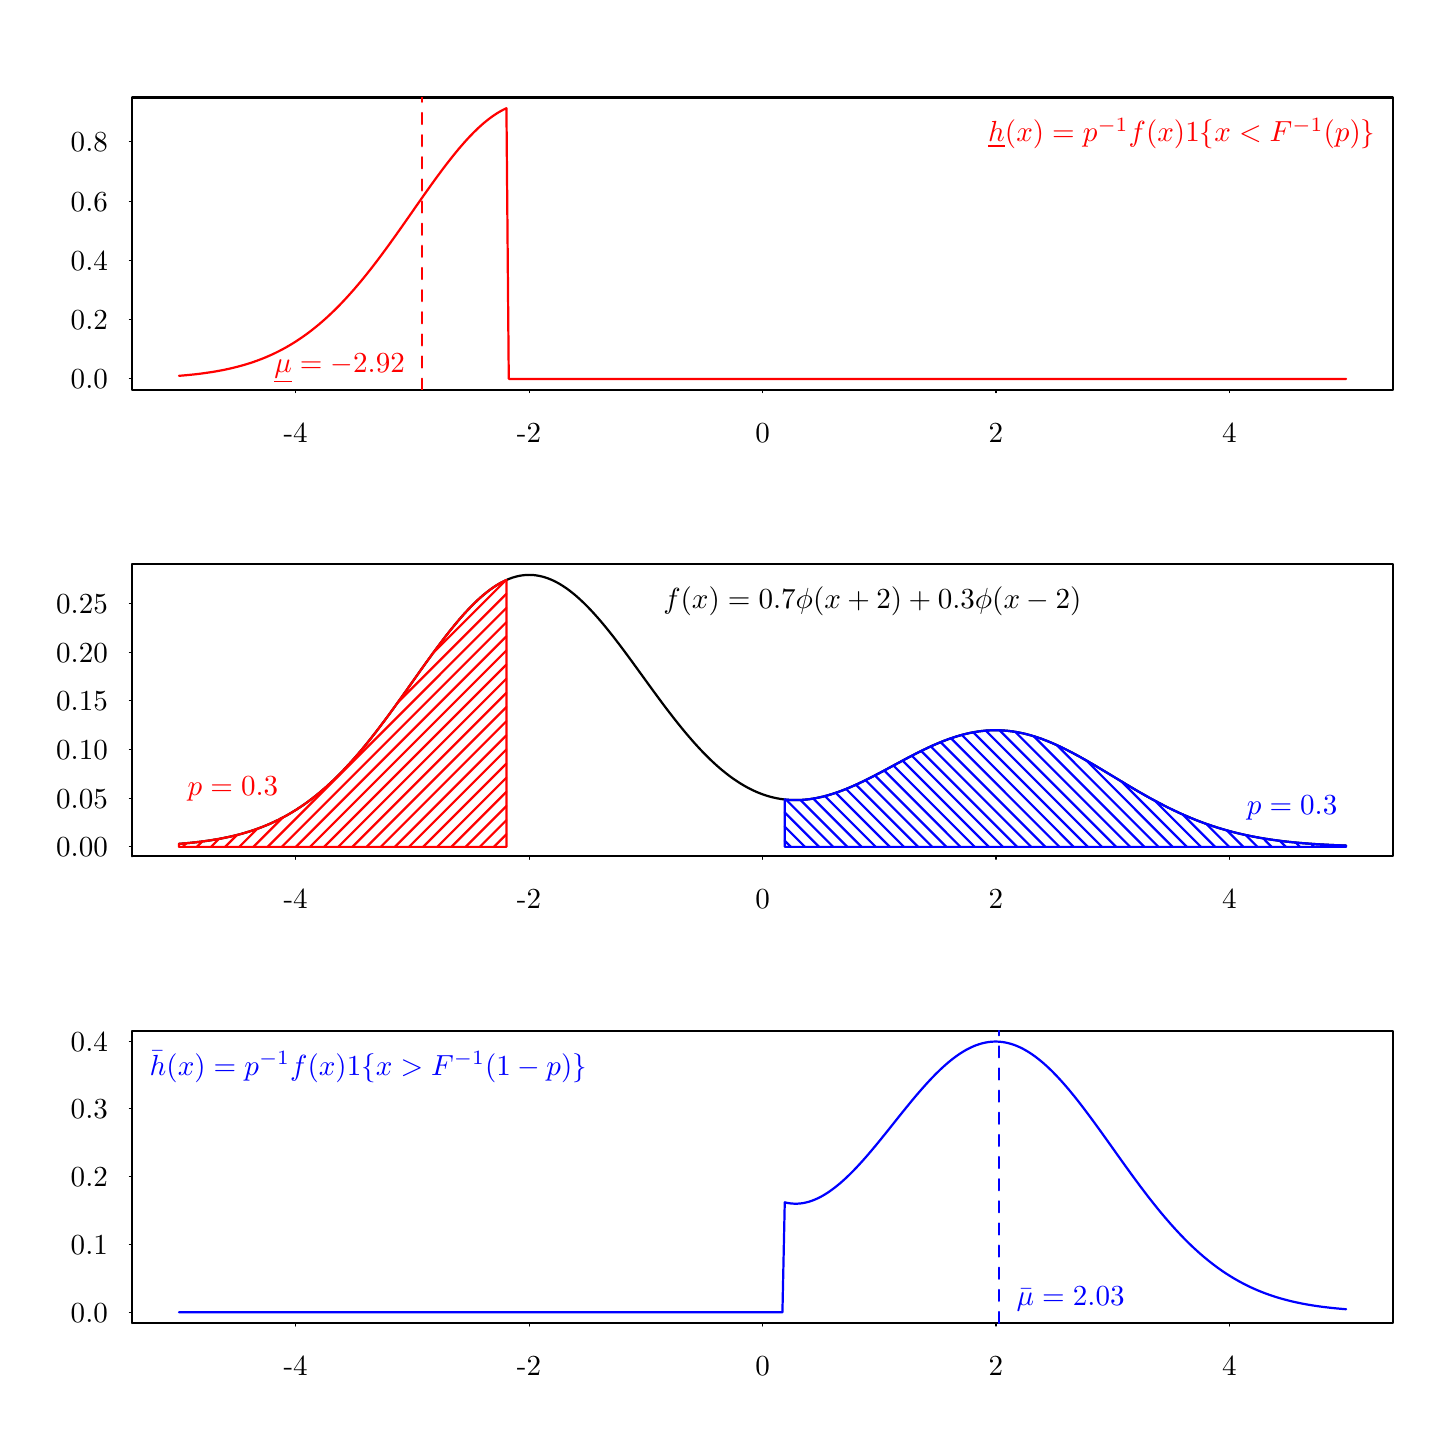
\begin{tikzpicture}[x=1pt,y=1pt]
\definecolor{fillColor}{RGB}{255,255,255}
\path[use as bounding box,fill=fillColor,fill opacity=0.00] (0,0) rectangle (505.89,505.89);
\begin{scope}
\path[clip] ( 37.80,375.06) rectangle (493.29,480.69);
\definecolor{drawColor}{RGB}{255,0,0}

\path[draw=drawColor,line width= 0.8pt,line join=round,line cap=round] ( 54.67,380.08) --
	( 55.52,380.15) --
	( 56.36,380.22) --
	( 57.21,380.30) --
	( 58.05,380.38) --
	( 58.90,380.46) --
	( 59.74,380.55) --
	( 60.59,380.64) --
	( 61.43,380.74) --
	( 62.28,380.84) --
	( 63.12,380.95) --
	( 63.97,381.07) --
	( 64.81,381.19) --
	( 65.66,381.31) --
	( 66.50,381.44) --
	( 67.35,381.58) --
	( 68.19,381.72) --
	( 69.04,381.88) --
	( 69.88,382.03) --
	( 70.73,382.20) --
	( 71.57,382.37) --
	( 72.42,382.55) --
	( 73.26,382.74) --
	( 74.11,382.94) --
	( 74.95,383.15) --
	( 75.80,383.36) --
	( 76.64,383.59) --
	( 77.49,383.82) --
	( 78.34,384.06) --
	( 79.18,384.32) --
	( 80.03,384.58) --
	( 80.87,384.86) --
	( 81.72,385.14) --
	( 82.56,385.44) --
	( 83.41,385.75) --
	( 84.25,386.07) --
	( 85.10,386.40) --
	( 85.94,386.75) --
	( 86.79,387.11) --
	( 87.63,387.48) --
	( 88.48,387.87) --
	( 89.32,388.26) --
	( 90.17,388.68) --
	( 91.01,389.10) --
	( 91.86,389.55) --
	( 92.70,390.00) --
	( 93.55,390.47) --
	( 94.39,390.96) --
	( 95.24,391.46) --
	( 96.08,391.98) --
	( 96.93,392.51) --
	( 97.77,393.06) --
	( 98.62,393.63) --
	( 99.47,394.22) --
	(100.31,394.82) --
	(101.16,395.43) --
	(102.00,396.07) --
	(102.85,396.72) --
	(103.69,397.39) --
	(104.54,398.08) --
	(105.38,398.78) --
	(106.23,399.50) --
	(107.07,400.24) --
	(107.92,401.00) --
	(108.76,401.78) --
	(109.61,402.57) --
	(110.45,403.38) --
	(111.30,404.21) --
	(112.14,405.06) --
	(112.99,405.92) --
	(113.83,406.81) --
	(114.68,407.71) --
	(115.52,408.62) --
	(116.37,409.56) --
	(117.21,410.51) --
	(118.06,411.47) --
	(118.90,412.46) --
	(119.75,413.46) --
	(120.59,414.47) --
	(121.44,415.50) --
	(122.29,416.55) --
	(123.13,417.60) --
	(123.98,418.68) --
	(124.82,419.76) --
	(125.67,420.86) --
	(126.51,421.97) --
	(127.36,423.10) --
	(128.20,424.23) --
	(129.05,425.38) --
	(129.89,426.53) --
	(130.74,427.69) --
	(131.58,428.87) --
	(132.43,430.05) --
	(133.27,431.23) --
	(134.12,432.43) --
	(134.96,433.62) --
	(135.81,434.83) --
	(136.65,436.03) --
	(137.50,437.24) --
	(138.34,438.45) --
	(139.19,439.66) --
	(140.03,440.88) --
	(140.88,442.09) --
	(141.72,443.29) --
	(142.57,444.50) --
	(143.41,445.70) --
	(144.26,446.89) --
	(145.11,448.08) --
	(145.95,449.26) --
	(146.80,450.44) --
	(147.64,451.60) --
	(148.49,452.75) --
	(149.33,453.89) --
	(150.18,455.02) --
	(151.02,456.13) --
	(151.87,457.23) --
	(152.71,458.31) --
	(153.56,459.38) --
	(154.40,460.43) --
	(155.25,461.45) --
	(156.09,462.46) --
	(156.94,463.44) --
	(157.78,464.41) --
	(158.63,465.35) --
	(159.47,466.26) --
	(160.32,467.15) --
	(161.16,468.01) --
	(162.01,468.84) --
	(162.85,469.65) --
	(163.70,470.42) --
	(164.54,471.17) --
	(165.39,471.88) --
	(166.24,472.56) --
	(167.08,473.21) --
	(167.93,473.83) --
	(168.77,474.41) --
	(169.62,474.95) --
	(170.46,475.47) --
	(171.31,475.94) --
	(172.15,476.38) --
	(173.00,476.78) --
	(173.84,378.97) --
	(174.69,378.97) --
	(175.53,378.97) --
	(176.38,378.97) --
	(177.22,378.97) --
	(178.07,378.97) --
	(178.91,378.97) --
	(179.76,378.97) --
	(180.60,378.97) --
	(181.45,378.97) --
	(182.29,378.97) --
	(183.14,378.97) --
	(183.98,378.97) --
	(184.83,378.97) --
	(185.67,378.97) --
	(186.52,378.97) --
	(187.36,378.97) --
	(188.21,378.97) --
	(189.06,378.97) --
	(189.90,378.97) --
	(190.75,378.97) --
	(191.59,378.97) --
	(192.44,378.97) --
	(193.28,378.97) --
	(194.13,378.97) --
	(194.97,378.97) --
	(195.82,378.97) --
	(196.66,378.97) --
	(197.51,378.97) --
	(198.35,378.97) --
	(199.20,378.97) --
	(200.04,378.97) --
	(200.89,378.97) --
	(201.73,378.97) --
	(202.58,378.97) --
	(203.42,378.97) --
	(204.27,378.97) --
	(205.11,378.97) --
	(205.96,378.97) --
	(206.80,378.97) --
	(207.65,378.97) --
	(208.49,378.97) --
	(209.34,378.97) --
	(210.19,378.97) --
	(211.03,378.97) --
	(211.88,378.97) --
	(212.72,378.97) --
	(213.57,378.97) --
	(214.41,378.97) --
	(215.26,378.97) --
	(216.10,378.97) --
	(216.95,378.97) --
	(217.79,378.97) --
	(218.64,378.97) --
	(219.48,378.97) --
	(220.33,378.97) --
	(221.17,378.97) --
	(222.02,378.97) --
	(222.86,378.97) --
	(223.71,378.97) --
	(224.55,378.97) --
	(225.40,378.97) --
	(226.24,378.97) --
	(227.09,378.97) --
	(227.93,378.97) --
	(228.78,378.97) --
	(229.62,378.97) --
	(230.47,378.97) --
	(231.31,378.97) --
	(232.16,378.97) --
	(233.01,378.97) --
	(233.85,378.97) --
	(234.70,378.97) --
	(235.54,378.97) --
	(236.39,378.97) --
	(237.23,378.97) --
	(238.08,378.97) --
	(238.92,378.97) --
	(239.77,378.97) --
	(240.61,378.97) --
	(241.46,378.97) --
	(242.30,378.97) --
	(243.15,378.97) --
	(243.99,378.97) --
	(244.84,378.97) --
	(245.68,378.97) --
	(246.53,378.97) --
	(247.37,378.97) --
	(248.22,378.97) --
	(249.06,378.97) --
	(249.91,378.97) --
	(250.75,378.97) --
	(251.60,378.97) --
	(252.44,378.97) --
	(253.29,378.97) --
	(254.13,378.97) --
	(254.98,378.97) --
	(255.83,378.97) --
	(256.67,378.97) --
	(257.52,378.97) --
	(258.36,378.97) --
	(259.21,378.97) --
	(260.05,378.97) --
	(260.90,378.97) --
	(261.74,378.97) --
	(262.59,378.97) --
	(263.43,378.97) --
	(264.28,378.97) --
	(265.12,378.97) --
	(265.97,378.97) --
	(266.81,378.97) --
	(267.66,378.97) --
	(268.50,378.97) --
	(269.35,378.97) --
	(270.19,378.97) --
	(271.04,378.97) --
	(271.88,378.97) --
	(272.73,378.97) --
	(273.57,378.97) --
	(274.42,378.97) --
	(275.26,378.97) --
	(276.11,378.97) --
	(276.96,378.97) --
	(277.80,378.97) --
	(278.65,378.97) --
	(279.49,378.97) --
	(280.34,378.97) --
	(281.18,378.97) --
	(282.03,378.97) --
	(282.87,378.97) --
	(283.72,378.97) --
	(284.56,378.97) --
	(285.41,378.97) --
	(286.25,378.97) --
	(287.10,378.97) --
	(287.94,378.97) --
	(288.79,378.97) --
	(289.63,378.97) --
	(290.48,378.97) --
	(291.32,378.97) --
	(292.17,378.97) --
	(293.01,378.97) --
	(293.86,378.97) --
	(294.70,378.97) --
	(295.55,378.97) --
	(296.39,378.97) --
	(297.24,378.97) --
	(298.08,378.97) --
	(298.93,378.97) --
	(299.78,378.97) --
	(300.62,378.97) --
	(301.47,378.97) --
	(302.31,378.97) --
	(303.16,378.97) --
	(304.00,378.97) --
	(304.85,378.97) --
	(305.69,378.97) --
	(306.54,378.97) --
	(307.38,378.97) --
	(308.23,378.97) --
	(309.07,378.97) --
	(309.92,378.97) --
	(310.76,378.97) --
	(311.61,378.97) --
	(312.45,378.97) --
	(313.30,378.97) --
	(314.14,378.97) --
	(314.99,378.97) --
	(315.83,378.97) --
	(316.68,378.97) --
	(317.52,378.97) --
	(318.37,378.97) --
	(319.21,378.97) --
	(320.06,378.97) --
	(320.90,378.97) --
	(321.75,378.97) --
	(322.60,378.97) --
	(323.44,378.97) --
	(324.29,378.97) --
	(325.13,378.97) --
	(325.98,378.97) --
	(326.82,378.97) --
	(327.67,378.97) --
	(328.51,378.97) --
	(329.36,378.97) --
	(330.20,378.97) --
	(331.05,378.97) --
	(331.89,378.97) --
	(332.74,378.97) --
	(333.58,378.97) --
	(334.43,378.97) --
	(335.27,378.97) --
	(336.12,378.97) --
	(336.96,378.97) --
	(337.81,378.97) --
	(338.65,378.97) --
	(339.50,378.97) --
	(340.34,378.97) --
	(341.19,378.97) --
	(342.03,378.97) --
	(342.88,378.97) --
	(343.73,378.97) --
	(344.57,378.97) --
	(345.42,378.97) --
	(346.26,378.97) --
	(347.11,378.97) --
	(347.95,378.97) --
	(348.80,378.97) --
	(349.64,378.97) --
	(350.49,378.97) --
	(351.33,378.97) --
	(352.18,378.97) --
	(353.02,378.97) --
	(353.87,378.97) --
	(354.71,378.97) --
	(355.56,378.97) --
	(356.40,378.97) --
	(357.25,378.97) --
	(358.09,378.97) --
	(358.94,378.97) --
	(359.78,378.97) --
	(360.63,378.97) --
	(361.47,378.97) --
	(362.32,378.97) --
	(363.16,378.97) --
	(364.01,378.97) --
	(364.85,378.97) --
	(365.70,378.97) --
	(366.55,378.97) --
	(367.39,378.97) --
	(368.24,378.97) --
	(369.08,378.97) --
	(369.93,378.97) --
	(370.77,378.97) --
	(371.62,378.97) --
	(372.46,378.97) --
	(373.31,378.97) --
	(374.15,378.97) --
	(375.00,378.97) --
	(375.84,378.97) --
	(376.69,378.97) --
	(377.53,378.97) --
	(378.38,378.97) --
	(379.22,378.97) --
	(380.07,378.97) --
	(380.91,378.97) --
	(381.76,378.97) --
	(382.60,378.97) --
	(383.45,378.97) --
	(384.29,378.97) --
	(385.14,378.97) --
	(385.98,378.97) --
	(386.83,378.97) --
	(387.68,378.97) --
	(388.52,378.97) --
	(389.37,378.97) --
	(390.21,378.97) --
	(391.06,378.97) --
	(391.90,378.97) --
	(392.75,378.97) --
	(393.59,378.97) --
	(394.44,378.97) --
	(395.28,378.97) --
	(396.13,378.97) --
	(396.97,378.97) --
	(397.82,378.97) --
	(398.66,378.97) --
	(399.51,378.97) --
	(400.35,378.97) --
	(401.20,378.97) --
	(402.04,378.97) --
	(402.89,378.97) --
	(403.73,378.97) --
	(404.58,378.97) --
	(405.42,378.97) --
	(406.27,378.97) --
	(407.11,378.97) --
	(407.96,378.97) --
	(408.80,378.97) --
	(409.65,378.97) --
	(410.50,378.97) --
	(411.34,378.97) --
	(412.19,378.97) --
	(413.03,378.97) --
	(413.88,378.97) --
	(414.72,378.97) --
	(415.57,378.97) --
	(416.41,378.97) --
	(417.26,378.97) --
	(418.10,378.97) --
	(418.95,378.97) --
	(419.79,378.97) --
	(420.64,378.97) --
	(421.48,378.97) --
	(422.33,378.97) --
	(423.17,378.97) --
	(424.02,378.97) --
	(424.86,378.97) --
	(425.71,378.97) --
	(426.55,378.97) --
	(427.40,378.97) --
	(428.24,378.97) --
	(429.09,378.97) --
	(429.93,378.97) --
	(430.78,378.97) --
	(431.62,378.97) --
	(432.47,378.97) --
	(433.32,378.97) --
	(434.16,378.97) --
	(435.01,378.97) --
	(435.85,378.97) --
	(436.70,378.97) --
	(437.54,378.97) --
	(438.39,378.97) --
	(439.23,378.97) --
	(440.08,378.97) --
	(440.92,378.97) --
	(441.77,378.97) --
	(442.61,378.97) --
	(443.46,378.97) --
	(444.30,378.97) --
	(445.15,378.97) --
	(445.99,378.97) --
	(446.84,378.97) --
	(447.68,378.97) --
	(448.53,378.97) --
	(449.37,378.97) --
	(450.22,378.97) --
	(451.06,378.97) --
	(451.91,378.97) --
	(452.75,378.97) --
	(453.60,378.97) --
	(454.45,378.97) --
	(455.29,378.97) --
	(456.14,378.97) --
	(456.98,378.97) --
	(457.83,378.97) --
	(458.67,378.97) --
	(459.52,378.97) --
	(460.36,378.97) --
	(461.21,378.97) --
	(462.05,378.97) --
	(462.90,378.97) --
	(463.74,378.97) --
	(464.59,378.97) --
	(465.43,378.97) --
	(466.28,378.97) --
	(467.12,378.97) --
	(467.97,378.97) --
	(468.81,378.97) --
	(469.66,378.97) --
	(470.50,378.97) --
	(471.35,378.97) --
	(472.19,378.97) --
	(473.04,378.97) --
	(473.88,378.97) --
	(474.73,378.97) --
	(475.57,378.97) --
	(476.42,378.97);
\end{scope}
\begin{scope}
\path[clip] (  0.00,  0.00) rectangle (505.89,505.89);
\definecolor{drawColor}{RGB}{0,0,0}

\path[draw=drawColor,line width= 0.4pt,line join=round,line cap=round] ( 96.84,375.06) -- (434.25,375.06);

\path[draw=drawColor,line width= 0.4pt,line join=round,line cap=round] ( 96.84,375.06) -- ( 96.84,374.00);

\path[draw=drawColor,line width= 0.4pt,line join=round,line cap=round] (181.19,375.06) -- (181.19,374.00);

\path[draw=drawColor,line width= 0.4pt,line join=round,line cap=round] (265.54,375.06) -- (265.54,374.00);

\path[draw=drawColor,line width= 0.4pt,line join=round,line cap=round] (349.89,375.06) -- (349.89,374.00);

\path[draw=drawColor,line width= 0.4pt,line join=round,line cap=round] (434.25,375.06) -- (434.25,374.00);

\node[text=drawColor,anchor=base,inner sep=0pt, outer sep=0pt, scale=  1.05] at ( 96.84,356.16) {-4};

\node[text=drawColor,anchor=base,inner sep=0pt, outer sep=0pt, scale=  1.05] at (181.19,356.16) {-2};

\node[text=drawColor,anchor=base,inner sep=0pt, outer sep=0pt, scale=  1.05] at (265.54,356.16) {0};

\node[text=drawColor,anchor=base,inner sep=0pt, outer sep=0pt, scale=  1.05] at (349.89,356.16) {2};

\node[text=drawColor,anchor=base,inner sep=0pt, outer sep=0pt, scale=  1.05] at (434.25,356.16) {4};

\path[draw=drawColor,line width= 0.4pt,line join=round,line cap=round] ( 37.80,378.97) -- ( 37.80,464.63);

\path[draw=drawColor,line width= 0.4pt,line join=round,line cap=round] ( 37.80,378.97) -- ( 36.74,378.97);

\path[draw=drawColor,line width= 0.4pt,line join=round,line cap=round] ( 37.80,400.39) -- ( 36.74,400.39);

\path[draw=drawColor,line width= 0.4pt,line join=round,line cap=round] ( 37.80,421.80) -- ( 36.74,421.80);

\path[draw=drawColor,line width= 0.4pt,line join=round,line cap=round] ( 37.80,443.21) -- ( 36.74,443.21);

\path[draw=drawColor,line width= 0.4pt,line join=round,line cap=round] ( 37.80,464.63) -- ( 36.74,464.63);

\node[text=drawColor,anchor=base east,inner sep=0pt, outer sep=0pt, scale=  1.05] at ( 28.98,375.36) {0.0};

\node[text=drawColor,anchor=base east,inner sep=0pt, outer sep=0pt, scale=  1.05] at ( 28.98,396.77) {0.2};

\node[text=drawColor,anchor=base east,inner sep=0pt, outer sep=0pt, scale=  1.05] at ( 28.98,418.18) {0.4};

\node[text=drawColor,anchor=base east,inner sep=0pt, outer sep=0pt, scale=  1.05] at ( 28.98,439.60) {0.6};

\node[text=drawColor,anchor=base east,inner sep=0pt, outer sep=0pt, scale=  1.05] at ( 28.98,461.01) {0.8};

\path[draw=drawColor,line width= 0.8pt,line join=round,line cap=round] ( 37.80,375.06) --
	(493.29,375.06) --
	(493.29,480.69) --
	( 37.80,480.69) --
	( 37.80,375.06);
\end{scope}
\begin{scope}
\path[clip] ( 37.80,375.06) rectangle (493.29,480.69);
\definecolor{drawColor}{RGB}{255,0,0}

\node[text=drawColor,anchor=base east,inner sep=0pt, outer sep=0pt, scale=  1.05] at (486.99,464.59) {$\underline{h}(x) = p^{-1}f(x) 1\{x < F^{-1}(p)\}$};

\path[draw=drawColor,line width= 0.8pt,dash pattern=on 4pt off 4pt ,line join=round,line cap=round] (142.60,375.06) -- (142.60,480.69);

\node[text=drawColor,anchor=base east,inner sep=0pt, outer sep=0pt, scale=  1.05] at (136.30,381.45) {$\underline{\mu} = -2.92$};
\end{scope}
\begin{scope}
\path[clip] ( 37.80,206.43) rectangle (493.29,312.06);
\definecolor{drawColor}{RGB}{0,0,0}

\path[draw=drawColor,line width= 0.8pt,line join=round,line cap=round] ( 54.67,210.97) --
	( 55.52,211.03) --
	( 56.36,211.10) --
	( 57.21,211.18) --
	( 58.05,211.26) --
	( 58.90,211.34) --
	( 59.74,211.43) --
	( 60.59,211.52) --
	( 61.43,211.62) --
	( 62.28,211.72) --
	( 63.12,211.83) --
	( 63.97,211.94) --
	( 64.81,212.06) --
	( 65.66,212.18) --
	( 66.50,212.31) --
	( 67.35,212.45) --
	( 68.19,212.59) --
	( 69.04,212.74) --
	( 69.88,212.89) --
	( 70.73,213.06) --
	( 71.57,213.23) --
	( 72.42,213.41) --
	( 73.26,213.59) --
	( 74.11,213.79) --
	( 74.95,213.99) --
	( 75.80,214.20) --
	( 76.64,214.42) --
	( 77.49,214.65) --
	( 78.34,214.90) --
	( 79.18,215.15) --
	( 80.03,215.41) --
	( 80.87,215.68) --
	( 81.72,215.96) --
	( 82.56,216.25) --
	( 83.41,216.56) --
	( 84.25,216.87) --
	( 85.10,217.20) --
	( 85.94,217.54) --
	( 86.79,217.90) --
	( 87.63,218.26) --
	( 88.48,218.64) --
	( 89.32,219.04) --
	( 90.17,219.44) --
	( 91.01,219.86) --
	( 91.86,220.30) --
	( 92.70,220.75) --
	( 93.55,221.21) --
	( 94.39,221.69) --
	( 95.24,222.19) --
	( 96.08,222.70) --
	( 96.93,223.23) --
	( 97.77,223.77) --
	( 98.62,224.33) --
	( 99.47,224.90) --
	(100.31,225.49) --
	(101.16,226.10) --
	(102.00,226.73) --
	(102.85,227.37) --
	(103.69,228.03) --
	(104.54,228.71) --
	(105.38,229.40) --
	(106.23,230.12) --
	(107.07,230.85) --
	(107.92,231.59) --
	(108.76,232.36) --
	(109.61,233.14) --
	(110.45,233.94) --
	(111.30,234.76) --
	(112.14,235.59) --
	(112.99,236.45) --
	(113.83,237.32) --
	(114.68,238.20) --
	(115.52,239.11) --
	(116.37,240.03) --
	(117.21,240.97) --
	(118.06,241.92) --
	(118.90,242.89) --
	(119.75,243.87) --
	(120.59,244.87) --
	(121.44,245.89) --
	(122.29,246.92) --
	(123.13,247.96) --
	(123.98,249.02) --
	(124.82,250.09) --
	(125.67,251.17) --
	(126.51,252.27) --
	(127.36,253.38) --
	(128.20,254.50) --
	(129.05,255.62) --
	(129.89,256.76) --
	(130.74,257.91) --
	(131.58,259.07) --
	(132.43,260.23) --
	(133.27,261.40) --
	(134.12,262.58) --
	(134.96,263.76) --
	(135.81,264.94) --
	(136.65,266.13) --
	(137.50,267.32) --
	(138.34,268.52) --
	(139.19,269.71) --
	(140.03,270.91) --
	(140.88,272.10) --
	(141.72,273.29) --
	(142.57,274.48) --
	(143.41,275.66) --
	(144.26,276.84) --
	(145.11,278.01) --
	(145.95,279.18) --
	(146.80,280.33) --
	(147.64,281.48) --
	(148.49,282.61) --
	(149.33,283.74) --
	(150.18,284.85) --
	(151.02,285.95) --
	(151.87,287.03) --
	(152.71,288.10) --
	(153.56,289.15) --
	(154.40,290.18) --
	(155.25,291.19) --
	(156.09,292.19) --
	(156.94,293.16) --
	(157.78,294.11) --
	(158.63,295.03) --
	(159.47,295.93) --
	(160.32,296.81) --
	(161.16,297.66) --
	(162.01,298.48) --
	(162.85,299.27) --
	(163.70,300.04) --
	(164.54,300.77) --
	(165.39,301.47) --
	(166.24,302.15) --
	(167.08,302.79) --
	(167.93,303.39) --
	(168.77,303.97) --
	(169.62,304.51) --
	(170.46,305.01) --
	(171.31,305.48) --
	(172.15,305.91) --
	(173.00,306.30) --
	(173.84,306.66) --
	(174.69,306.98) --
	(175.53,307.26) --
	(176.38,307.50) --
	(177.22,307.71) --
	(178.07,307.88) --
	(178.91,308.00) --
	(179.76,308.09) --
	(180.60,308.14) --
	(181.45,308.15) --
	(182.29,308.12) --
	(183.14,308.05) --
	(183.98,307.94) --
	(184.83,307.79) --
	(185.67,307.60) --
	(186.52,307.38) --
	(187.36,307.11) --
	(188.21,306.81) --
	(189.06,306.47) --
	(189.90,306.10) --
	(190.75,305.68) --
	(191.59,305.23) --
	(192.44,304.75) --
	(193.28,304.22) --
	(194.13,303.67) --
	(194.97,303.08) --
	(195.82,302.46) --
	(196.66,301.80) --
	(197.51,301.12) --
	(198.35,300.40) --
	(199.20,299.65) --
	(200.04,298.87) --
	(200.89,298.07) --
	(201.73,297.24) --
	(202.58,296.38) --
	(203.42,295.49) --
	(204.27,294.59) --
	(205.11,293.65) --
	(205.96,292.70) --
	(206.80,291.73) --
	(207.65,290.73) --
	(208.49,289.72) --
	(209.34,288.68) --
	(210.19,287.63) --
	(211.03,286.57) --
	(211.88,285.49) --
	(212.72,284.40) --
	(213.57,283.29) --
	(214.41,282.18) --
	(215.26,281.05) --
	(216.10,279.91) --
	(216.95,278.77) --
	(217.79,277.62) --
	(218.64,276.46) --
	(219.48,275.30) --
	(220.33,274.14) --
	(221.17,272.97) --
	(222.02,271.81) --
	(222.86,270.64) --
	(223.71,269.47) --
	(224.55,268.31) --
	(225.40,267.15) --
	(226.24,265.99) --
	(227.09,264.84) --
	(227.93,263.69) --
	(228.78,262.55) --
	(229.62,261.42) --
	(230.47,260.29) --
	(231.31,259.18) --
	(232.16,258.08) --
	(233.01,256.98) --
	(233.85,255.90) --
	(234.70,254.83) --
	(235.54,253.78) --
	(236.39,252.74) --
	(237.23,251.71) --
	(238.08,250.70) --
	(238.92,249.71) --
	(239.77,248.73) --
	(240.61,247.77) --
	(241.46,246.82) --
	(242.30,245.90) --
	(243.15,244.99) --
	(243.99,244.10) --
	(244.84,243.24) --
	(245.68,242.39) --
	(246.53,241.56) --
	(247.37,240.76) --
	(248.22,239.97) --
	(249.06,239.21) --
	(249.91,238.47) --
	(250.75,237.75) --
	(251.60,237.05) --
	(252.44,236.38) --
	(253.29,235.73) --
	(254.13,235.10) --
	(254.98,234.49) --
	(255.83,233.91) --
	(256.67,233.35) --
	(257.52,232.81) --
	(258.36,232.30) --
	(259.21,231.81) --
	(260.05,231.34) --
	(260.90,230.90) --
	(261.74,230.48) --
	(262.59,230.08) --
	(263.43,229.70) --
	(264.28,229.35) --
	(265.12,229.03) --
	(265.97,228.72) --
	(266.81,228.44) --
	(267.66,228.18) --
	(268.50,227.94) --
	(269.35,227.73) --
	(270.19,227.54) --
	(271.04,227.37) --
	(271.88,227.22) --
	(272.73,227.09) --
	(273.57,226.99) --
	(274.42,226.90) --
	(275.26,226.84) --
	(276.11,226.80) --
	(276.96,226.78) --
	(277.80,226.77) --
	(278.65,226.79) --
	(279.49,226.83) --
	(280.34,226.88) --
	(281.18,226.96) --
	(282.03,227.05) --
	(282.87,227.16) --
	(283.72,227.29) --
	(284.56,227.44) --
	(285.41,227.60) --
	(286.25,227.78) --
	(287.10,227.97) --
	(287.94,228.18) --
	(288.79,228.41) --
	(289.63,228.65) --
	(290.48,228.91) --
	(291.32,229.18) --
	(292.17,229.46) --
	(293.01,229.76) --
	(293.86,230.07) --
	(294.70,230.39) --
	(295.55,230.72) --
	(296.39,231.07) --
	(297.24,231.42) --
	(298.08,231.79) --
	(298.93,232.16) --
	(299.78,232.55) --
	(300.62,232.94) --
	(301.47,233.34) --
	(302.31,233.75) --
	(303.16,234.16) --
	(304.00,234.59) --
	(304.85,235.01) --
	(305.69,235.45) --
	(306.54,235.89) --
	(307.38,236.33) --
	(308.23,236.78) --
	(309.07,237.23) --
	(309.92,237.68) --
	(310.76,238.13) --
	(311.61,238.59) --
	(312.45,239.05) --
	(313.30,239.50) --
	(314.14,239.96) --
	(314.99,240.41) --
	(315.83,240.87) --
	(316.68,241.32) --
	(317.52,241.77) --
	(318.37,242.22) --
	(319.21,242.66) --
	(320.06,243.10) --
	(320.90,243.53) --
	(321.75,243.96) --
	(322.60,244.38) --
	(323.44,244.80) --
	(324.29,245.21) --
	(325.13,245.61) --
	(325.98,246.00) --
	(326.82,246.39) --
	(327.67,246.76) --
	(328.51,247.13) --
	(329.36,247.48) --
	(330.20,247.83) --
	(331.05,248.16) --
	(331.89,248.49) --
	(332.74,248.80) --
	(333.58,249.09) --
	(334.43,249.38) --
	(335.27,249.65) --
	(336.12,249.91) --
	(336.96,250.16) --
	(337.81,250.39) --
	(338.65,250.61) --
	(339.50,250.81) --
	(340.34,251.00) --
	(341.19,251.17) --
	(342.03,251.33) --
	(342.88,251.47) --
	(343.73,251.60) --
	(344.57,251.71) --
	(345.42,251.80) --
	(346.26,251.88) --
	(347.11,251.94) --
	(347.95,251.98) --
	(348.80,252.01) --
	(349.64,252.02) --
	(350.49,252.01) --
	(351.33,251.99) --
	(352.18,251.95) --
	(353.02,251.89) --
	(353.87,251.82) --
	(354.71,251.73) --
	(355.56,251.63) --
	(356.40,251.51) --
	(357.25,251.37) --
	(358.09,251.21) --
	(358.94,251.04) --
	(359.78,250.86) --
	(360.63,250.66) --
	(361.47,250.44) --
	(362.32,250.21) --
	(363.16,249.96) --
	(364.01,249.70) --
	(364.85,249.43) --
	(365.70,249.14) --
	(366.55,248.84) --
	(367.39,248.52) --
	(368.24,248.19) --
	(369.08,247.85) --
	(369.93,247.50) --
	(370.77,247.13) --
	(371.62,246.76) --
	(372.46,246.37) --
	(373.31,245.98) --
	(374.15,245.57) --
	(375.00,245.15) --
	(375.84,244.73) --
	(376.69,244.29) --
	(377.53,243.85) --
	(378.38,243.40) --
	(379.22,242.94) --
	(380.07,242.48) --
	(380.91,242.01) --
	(381.76,241.53) --
	(382.60,241.05) --
	(383.45,240.56) --
	(384.29,240.07) --
	(385.14,239.58) --
	(385.98,239.08) --
	(386.83,238.57) --
	(387.68,238.07) --
	(388.52,237.56) --
	(389.37,237.05) --
	(390.21,236.54) --
	(391.06,236.03) --
	(391.90,235.52) --
	(392.75,235.01) --
	(393.59,234.50) --
	(394.44,233.98) --
	(395.28,233.48) --
	(396.13,232.97) --
	(396.97,232.46) --
	(397.82,231.96) --
	(398.66,231.46) --
	(399.51,230.96) --
	(400.35,230.46) --
	(401.20,229.97) --
	(402.04,229.48) --
	(402.89,229.00) --
	(403.73,228.52) --
	(404.58,228.04) --
	(405.42,227.57) --
	(406.27,227.11) --
	(407.11,226.65) --
	(407.96,226.20) --
	(408.80,225.75) --
	(409.65,225.31) --
	(410.50,224.87) --
	(411.34,224.45) --
	(412.19,224.02) --
	(413.03,223.61) --
	(413.88,223.20) --
	(414.72,222.80) --
	(415.57,222.40) --
	(416.41,222.02) --
	(417.26,221.64) --
	(418.10,221.26) --
	(418.95,220.90) --
	(419.79,220.54) --
	(420.64,220.19) --
	(421.48,219.85) --
	(422.33,219.51) --
	(423.17,219.18) --
	(424.02,218.86) --
	(424.86,218.55) --
	(425.71,218.24) --
	(426.55,217.95) --
	(427.40,217.66) --
	(428.24,217.37) --
	(429.09,217.10) --
	(429.93,216.83) --
	(430.78,216.57) --
	(431.62,216.32) --
	(432.47,216.07) --
	(433.32,215.83) --
	(434.16,215.60) --
	(435.01,215.37) --
	(435.85,215.15) --
	(436.70,214.94) --
	(437.54,214.73) --
	(438.39,214.53) --
	(439.23,214.34) --
	(440.08,214.16) --
	(440.92,213.98) --
	(441.77,213.80) --
	(442.61,213.63) --
	(443.46,213.47) --
	(444.30,213.31) --
	(445.15,213.16) --
	(445.99,213.02) --
	(446.84,212.87) --
	(447.68,212.74) --
	(448.53,212.61) --
	(449.37,212.48) --
	(450.22,212.36) --
	(451.06,212.25) --
	(451.91,212.13) --
	(452.75,212.03) --
	(453.60,211.92) --
	(454.45,211.82) --
	(455.29,211.73) --
	(456.14,211.64) --
	(456.98,211.55) --
	(457.83,211.47) --
	(458.67,211.39) --
	(459.52,211.31) --
	(460.36,211.24) --
	(461.21,211.17) --
	(462.05,211.10) --
	(462.90,211.04) --
	(463.74,210.98) --
	(464.59,210.92) --
	(465.43,210.86) --
	(466.28,210.81) --
	(467.12,210.76) --
	(467.97,210.71) --
	(468.81,210.67) --
	(469.66,210.62) --
	(470.50,210.58) --
	(471.35,210.54) --
	(472.19,210.50) --
	(473.04,210.47) --
	(473.88,210.43) --
	(474.73,210.40) --
	(475.57,210.37) --
	(476.42,210.34);
\end{scope}
\begin{scope}
\path[clip] (  0.00,  0.00) rectangle (505.89,505.89);
\definecolor{drawColor}{RGB}{0,0,0}

\path[draw=drawColor,line width= 0.4pt,line join=round,line cap=round] ( 96.84,206.43) -- (434.25,206.43);

\path[draw=drawColor,line width= 0.4pt,line join=round,line cap=round] ( 96.84,206.43) -- ( 96.84,205.37);

\path[draw=drawColor,line width= 0.4pt,line join=round,line cap=round] (181.19,206.43) -- (181.19,205.37);

\path[draw=drawColor,line width= 0.4pt,line join=round,line cap=round] (265.54,206.43) -- (265.54,205.37);

\path[draw=drawColor,line width= 0.4pt,line join=round,line cap=round] (349.89,206.43) -- (349.89,205.37);

\path[draw=drawColor,line width= 0.4pt,line join=round,line cap=round] (434.25,206.43) -- (434.25,205.37);

\node[text=drawColor,anchor=base,inner sep=0pt, outer sep=0pt, scale=  1.05] at ( 96.84,187.53) {-4};

\node[text=drawColor,anchor=base,inner sep=0pt, outer sep=0pt, scale=  1.05] at (181.19,187.53) {-2};

\node[text=drawColor,anchor=base,inner sep=0pt, outer sep=0pt, scale=  1.05] at (265.54,187.53) {0};

\node[text=drawColor,anchor=base,inner sep=0pt, outer sep=0pt, scale=  1.05] at (349.89,187.53) {2};

\node[text=drawColor,anchor=base,inner sep=0pt, outer sep=0pt, scale=  1.05] at (434.25,187.53) {4};

\path[draw=drawColor,line width= 0.4pt,line join=round,line cap=round] ( 37.80,209.87) -- ( 37.80,297.84);

\path[draw=drawColor,line width= 0.4pt,line join=round,line cap=round] ( 37.80,209.87) -- ( 36.74,209.87);

\path[draw=drawColor,line width= 0.4pt,line join=round,line cap=round] ( 37.80,227.47) -- ( 36.74,227.47);

\path[draw=drawColor,line width= 0.4pt,line join=round,line cap=round] ( 37.80,245.06) -- ( 36.74,245.06);

\path[draw=drawColor,line width= 0.4pt,line join=round,line cap=round] ( 37.80,262.65) -- ( 36.74,262.65);

\path[draw=drawColor,line width= 0.4pt,line join=round,line cap=round] ( 37.80,280.25) -- ( 36.74,280.25);

\path[draw=drawColor,line width= 0.4pt,line join=round,line cap=round] ( 37.80,297.84) -- ( 36.74,297.84);

\node[text=drawColor,anchor=base east,inner sep=0pt, outer sep=0pt, scale=  1.05] at ( 28.98,206.26) {0.00};

\node[text=drawColor,anchor=base east,inner sep=0pt, outer sep=0pt, scale=  1.05] at ( 28.98,223.85) {0.05};

\node[text=drawColor,anchor=base east,inner sep=0pt, outer sep=0pt, scale=  1.05] at ( 28.98,241.44) {0.10};

\node[text=drawColor,anchor=base east,inner sep=0pt, outer sep=0pt, scale=  1.05] at ( 28.98,259.04) {0.15};

\node[text=drawColor,anchor=base east,inner sep=0pt, outer sep=0pt, scale=  1.05] at ( 28.98,276.63) {0.20};

\node[text=drawColor,anchor=base east,inner sep=0pt, outer sep=0pt, scale=  1.05] at ( 28.98,294.22) {0.25};

\path[draw=drawColor,line width= 0.8pt,line join=round,line cap=round] ( 37.80,206.43) --
	(493.29,206.43) --
	(493.29,312.06) --
	( 37.80,312.06) --
	( 37.80,206.43);
\end{scope}
\begin{scope}
\path[clip] ( 37.80,206.43) rectangle (493.29,312.06);
\definecolor{drawColor}{RGB}{255,0,0}

\path[draw=drawColor,line width= 0.8pt,line join=round,line cap=round] ( 56.02,209.87) -- ( 57.34,211.19);

\path[draw=drawColor,line width= 0.8pt,line join=round,line cap=round] ( 61.13,209.87) -- ( 63.08,211.82);

\path[draw=drawColor,line width= 0.8pt,line join=round,line cap=round] ( 66.24,209.87) -- ( 69.12,212.75);

\path[draw=drawColor,line width= 0.8pt,line join=round,line cap=round] ( 71.36,209.87) -- ( 75.64,214.16);

\path[draw=drawColor,line width= 0.8pt,line join=round,line cap=round] ( 76.47,209.87) -- ( 83.00,216.41);

\path[draw=drawColor,line width= 0.8pt,line join=round,line cap=round] (146.45,279.86) -- (172.80,306.21);

\path[draw=drawColor,line width= 0.8pt,line join=round,line cap=round] ( 81.58,209.87) -- ( 92.16,220.46);

\path[draw=drawColor,line width= 0.8pt,line join=round,line cap=round] (133.71,262.01) -- (173.00,301.30);

\path[draw=drawColor,line width= 0.8pt,line join=round,line cap=round] ( 86.69,209.87) -- (173.00,296.19);

\path[draw=drawColor,line width= 0.8pt,line join=round,line cap=round] ( 91.80,209.87) -- (173.00,291.07);

\path[draw=drawColor,line width= 0.8pt,line join=round,line cap=round] ( 96.91,209.87) -- (173.00,285.96);

\path[draw=drawColor,line width= 0.8pt,line join=round,line cap=round] (102.02,209.87) -- (173.00,280.85);

\path[draw=drawColor,line width= 0.8pt,line join=round,line cap=round] (107.13,209.87) -- (173.00,275.74);

\path[draw=drawColor,line width= 0.8pt,line join=round,line cap=round] (112.24,209.87) -- (173.00,270.63);

\path[draw=drawColor,line width= 0.8pt,line join=round,line cap=round] (117.35,209.87) -- (173.00,265.52);

\path[draw=drawColor,line width= 0.8pt,line join=round,line cap=round] (122.46,209.87) -- (173.00,260.41);

\path[draw=drawColor,line width= 0.8pt,line join=round,line cap=round] (127.57,209.87) -- (173.00,255.30);

\path[draw=drawColor,line width= 0.8pt,line join=round,line cap=round] (132.68,209.87) -- (173.00,250.19);

\path[draw=drawColor,line width= 0.8pt,line join=round,line cap=round] (137.79,209.87) -- (173.00,245.08);

\path[draw=drawColor,line width= 0.8pt,line join=round,line cap=round] (142.90,209.87) -- (173.00,239.97);

\path[draw=drawColor,line width= 0.8pt,line join=round,line cap=round] (148.01,209.87) -- (173.00,234.86);

\path[draw=drawColor,line width= 0.8pt,line join=round,line cap=round] (153.12,209.87) -- (173.00,229.75);

\path[draw=drawColor,line width= 0.8pt,line join=round,line cap=round] (158.23,209.87) -- (173.00,224.64);

\path[draw=drawColor,line width= 0.8pt,line join=round,line cap=round] (163.34,209.87) -- (173.00,219.53);

\path[draw=drawColor,line width= 0.8pt,line join=round,line cap=round] (168.45,209.87) -- (173.00,214.42);

\path[draw=drawColor,line width= 0.8pt,line join=round,line cap=round] ( 54.67,209.87) --
	( 55.52,209.87) --
	( 56.36,209.87) --
	( 57.21,209.87) --
	( 58.05,209.87) --
	( 58.90,209.87) --
	( 59.74,209.87) --
	( 60.59,209.87) --
	( 61.43,209.87) --
	( 62.28,209.87) --
	( 63.12,209.87) --
	( 63.97,209.87) --
	( 64.81,209.87) --
	( 65.66,209.87) --
	( 66.50,209.87) --
	( 67.35,209.87) --
	( 68.19,209.87) --
	( 69.04,209.87) --
	( 69.88,209.87) --
	( 70.73,209.87) --
	( 71.57,209.87) --
	( 72.42,209.87) --
	( 73.26,209.87) --
	( 74.11,209.87) --
	( 74.95,209.87) --
	( 75.80,209.87) --
	( 76.64,209.87) --
	( 77.49,209.87) --
	( 78.34,209.87) --
	( 79.18,209.87) --
	( 80.03,209.87) --
	( 80.87,209.87) --
	( 81.72,209.87) --
	( 82.56,209.87) --
	( 83.41,209.87) --
	( 84.25,209.87) --
	( 85.10,209.87) --
	( 85.94,209.87) --
	( 86.79,209.87) --
	( 87.63,209.87) --
	( 88.48,209.87) --
	( 89.32,209.87) --
	( 90.17,209.87) --
	( 91.01,209.87) --
	( 91.86,209.87) --
	( 92.70,209.87) --
	( 93.55,209.87) --
	( 94.39,209.87) --
	( 95.24,209.87) --
	( 96.08,209.87) --
	( 96.93,209.87) --
	( 97.77,209.87) --
	( 98.62,209.87) --
	( 99.47,209.87) --
	(100.31,209.87) --
	(101.16,209.87) --
	(102.00,209.87) --
	(102.85,209.87) --
	(103.69,209.87) --
	(104.54,209.87) --
	(105.38,209.87) --
	(106.23,209.87) --
	(107.07,209.87) --
	(107.92,209.87) --
	(108.76,209.87) --
	(109.61,209.87) --
	(110.45,209.87) --
	(111.30,209.87) --
	(112.14,209.87) --
	(112.99,209.87) --
	(113.83,209.87) --
	(114.68,209.87) --
	(115.52,209.87) --
	(116.37,209.87) --
	(117.21,209.87) --
	(118.06,209.87) --
	(118.90,209.87) --
	(119.75,209.87) --
	(120.59,209.87) --
	(121.44,209.87) --
	(122.29,209.87) --
	(123.13,209.87) --
	(123.98,209.87) --
	(124.82,209.87) --
	(125.67,209.87) --
	(126.51,209.87) --
	(127.36,209.87) --
	(128.20,209.87) --
	(129.05,209.87) --
	(129.89,209.87) --
	(130.74,209.87) --
	(131.58,209.87) --
	(132.43,209.87) --
	(133.27,209.87) --
	(134.12,209.87) --
	(134.96,209.87) --
	(135.81,209.87) --
	(136.65,209.87) --
	(137.50,209.87) --
	(138.34,209.87) --
	(139.19,209.87) --
	(140.03,209.87) --
	(140.88,209.87) --
	(141.72,209.87) --
	(142.57,209.87) --
	(143.41,209.87) --
	(144.26,209.87) --
	(145.11,209.87) --
	(145.95,209.87) --
	(146.80,209.87) --
	(147.64,209.87) --
	(148.49,209.87) --
	(149.33,209.87) --
	(150.18,209.87) --
	(151.02,209.87) --
	(151.87,209.87) --
	(152.71,209.87) --
	(153.56,209.87) --
	(154.40,209.87) --
	(155.25,209.87) --
	(156.09,209.87) --
	(156.94,209.87) --
	(157.78,209.87) --
	(158.63,209.87) --
	(159.47,209.87) --
	(160.32,209.87) --
	(161.16,209.87) --
	(162.01,209.87) --
	(162.85,209.87) --
	(163.70,209.87) --
	(164.54,209.87) --
	(165.39,209.87) --
	(166.24,209.87) --
	(167.08,209.87) --
	(167.93,209.87) --
	(168.77,209.87) --
	(169.62,209.87) --
	(170.46,209.87) --
	(171.31,209.87) --
	(172.15,209.87) --
	(173.00,209.87) --
	(173.00,306.30) --
	(172.15,305.91) --
	(171.31,305.48) --
	(170.46,305.01) --
	(169.62,304.51) --
	(168.77,303.97) --
	(167.93,303.39) --
	(167.08,302.79) --
	(166.24,302.15) --
	(165.39,301.47) --
	(164.54,300.77) --
	(163.70,300.04) --
	(162.85,299.27) --
	(162.01,298.48) --
	(161.16,297.66) --
	(160.32,296.81) --
	(159.47,295.93) --
	(158.63,295.03) --
	(157.78,294.11) --
	(156.94,293.16) --
	(156.09,292.19) --
	(155.25,291.19) --
	(154.40,290.18) --
	(153.56,289.15) --
	(152.71,288.10) --
	(151.87,287.03) --
	(151.02,285.95) --
	(150.18,284.85) --
	(149.33,283.74) --
	(148.49,282.61) --
	(147.64,281.48) --
	(146.80,280.33) --
	(145.95,279.18) --
	(145.11,278.01) --
	(144.26,276.84) --
	(143.41,275.66) --
	(142.57,274.48) --
	(141.72,273.29) --
	(140.88,272.10) --
	(140.03,270.91) --
	(139.19,269.71) --
	(138.34,268.52) --
	(137.50,267.32) --
	(136.65,266.13) --
	(135.81,264.94) --
	(134.96,263.76) --
	(134.12,262.58) --
	(133.27,261.40) --
	(132.43,260.23) --
	(131.58,259.07) --
	(130.74,257.91) --
	(129.89,256.76) --
	(129.05,255.62) --
	(128.20,254.50) --
	(127.36,253.38) --
	(126.51,252.27) --
	(125.67,251.17) --
	(124.82,250.09) --
	(123.98,249.02) --
	(123.13,247.96) --
	(122.29,246.92) --
	(121.44,245.89) --
	(120.59,244.87) --
	(119.75,243.87) --
	(118.90,242.89) --
	(118.06,241.92) --
	(117.21,240.97) --
	(116.37,240.03) --
	(115.52,239.11) --
	(114.68,238.20) --
	(113.83,237.32) --
	(112.99,236.45) --
	(112.14,235.59) --
	(111.30,234.76) --
	(110.45,233.94) --
	(109.61,233.14) --
	(108.76,232.36) --
	(107.92,231.59) --
	(107.07,230.85) --
	(106.23,230.12) --
	(105.38,229.40) --
	(104.54,228.71) --
	(103.69,228.03) --
	(102.85,227.37) --
	(102.00,226.73) --
	(101.16,226.10) --
	(100.31,225.49) --
	( 99.47,224.90) --
	( 98.62,224.33) --
	( 97.77,223.77) --
	( 96.93,223.23) --
	( 96.08,222.70) --
	( 95.24,222.19) --
	( 94.39,221.69) --
	( 93.55,221.21) --
	( 92.70,220.75) --
	( 91.86,220.30) --
	( 91.01,219.86) --
	( 90.17,219.44) --
	( 89.32,219.04) --
	( 88.48,218.64) --
	( 87.63,218.26) --
	( 86.79,217.90) --
	( 85.94,217.54) --
	( 85.10,217.20) --
	( 84.25,216.87) --
	( 83.41,216.56) --
	( 82.56,216.25) --
	( 81.72,215.96) --
	( 80.87,215.68) --
	( 80.03,215.41) --
	( 79.18,215.15) --
	( 78.34,214.90) --
	( 77.49,214.65) --
	( 76.64,214.42) --
	( 75.80,214.20) --
	( 74.95,213.99) --
	( 74.11,213.79) --
	( 73.26,213.59) --
	( 72.42,213.41) --
	( 71.57,213.23) --
	( 70.73,213.06) --
	( 69.88,212.89) --
	( 69.04,212.74) --
	( 68.19,212.59) --
	( 67.35,212.45) --
	( 66.50,212.31) --
	( 65.66,212.18) --
	( 64.81,212.06) --
	( 63.97,211.94) --
	( 63.12,211.83) --
	( 62.28,211.72) --
	( 61.43,211.62) --
	( 60.59,211.52) --
	( 59.74,211.43) --
	( 58.90,211.34) --
	( 58.05,211.26) --
	( 57.21,211.18) --
	( 56.36,211.10) --
	( 55.52,211.03) --
	( 54.67,210.97) --
	( 54.67,209.87);

\node[text=drawColor,anchor=base east,inner sep=0pt, outer sep=0pt, scale=  1.05] at ( 90.54,228.58) {$p = 0.3$};
\definecolor{drawColor}{RGB}{0,0,255}

\path[draw=drawColor,line width= 0.8pt,line join=round,line cap=round] (275.77,209.87) -- (273.57,212.07);

\path[draw=drawColor,line width= 0.8pt,line join=round,line cap=round] (280.88,209.87) -- (273.57,217.18);

\path[draw=drawColor,line width= 0.8pt,line join=round,line cap=round] (285.99,209.87) -- (273.57,222.29);

\path[draw=drawColor,line width= 0.8pt,line join=round,line cap=round] (291.10,209.87) -- (274.03,226.94);

\path[draw=drawColor,line width= 0.8pt,line join=round,line cap=round] (296.21,209.87) -- (279.26,226.82);

\path[draw=drawColor,line width= 0.8pt,line join=round,line cap=round] (301.32,209.87) -- (283.87,227.32);

\path[draw=drawColor,line width= 0.8pt,line join=round,line cap=round] (306.43,209.87) -- (288.08,228.22);

\path[draw=drawColor,line width= 0.8pt,line join=round,line cap=round] (311.54,209.87) -- (292.01,229.41);

\path[draw=drawColor,line width= 0.8pt,line join=round,line cap=round] (316.65,209.87) -- (295.73,230.79);

\path[draw=drawColor,line width= 0.8pt,line join=round,line cap=round] (321.76,209.87) -- (299.30,232.33);

\path[draw=drawColor,line width= 0.8pt,line join=round,line cap=round] (326.87,209.87) -- (302.77,233.97);

\path[draw=drawColor,line width= 0.8pt,line join=round,line cap=round] (331.98,209.87) -- (306.16,235.69);

\path[draw=drawColor,line width= 0.8pt,line join=round,line cap=round] (337.09,209.87) -- (309.51,237.46);

\path[draw=drawColor,line width= 0.8pt,line join=round,line cap=round] (342.20,209.87) -- (312.83,239.25);

\path[draw=drawColor,line width= 0.8pt,line join=round,line cap=round] (347.31,209.87) -- (316.15,241.04);

\path[draw=drawColor,line width= 0.8pt,line join=round,line cap=round] (352.42,209.87) -- (319.49,242.80);

\path[draw=drawColor,line width= 0.8pt,line join=round,line cap=round] (357.53,209.87) -- (322.88,244.52);

\path[draw=drawColor,line width= 0.8pt,line join=round,line cap=round] (362.64,209.87) -- (326.35,246.17);

\path[draw=drawColor,line width= 0.8pt,line join=round,line cap=round] (367.75,209.87) -- (329.91,247.71);

\path[draw=drawColor,line width= 0.8pt,line join=round,line cap=round] (372.86,209.87) -- (333.63,249.11);

\path[draw=drawColor,line width= 0.8pt,line join=round,line cap=round] (377.97,209.87) -- (337.53,250.32);

\path[draw=drawColor,line width= 0.8pt,line join=round,line cap=round] (383.08,209.87) -- (341.69,251.27);

\path[draw=drawColor,line width= 0.8pt,line join=round,line cap=round] (388.19,209.87) -- (346.20,251.87);

\path[draw=drawColor,line width= 0.8pt,line join=round,line cap=round] (393.30,209.87) -- (351.18,251.99);

\path[draw=drawColor,line width= 0.8pt,line join=round,line cap=round] (398.41,209.87) -- (356.85,251.43);

\path[draw=drawColor,line width= 0.8pt,line join=round,line cap=round] (403.52,209.87) -- (363.56,249.84);

\path[draw=drawColor,line width= 0.8pt,line join=round,line cap=round] (408.63,209.87) -- (371.86,246.65);

\path[draw=drawColor,line width= 0.8pt,line join=round,line cap=round] (413.74,209.87) -- (382.52,241.10);

\path[draw=drawColor,line width= 0.8pt,line join=round,line cap=round] (418.85,209.87) -- (395.21,233.52);

\path[draw=drawColor,line width= 0.8pt,line join=round,line cap=round] (423.96,209.87) -- (407.27,226.57);

\path[draw=drawColor,line width= 0.8pt,line join=round,line cap=round] (429.07,209.87) -- (417.36,221.59);

\path[draw=drawColor,line width= 0.8pt,line join=round,line cap=round] (434.18,209.87) -- (425.87,218.19);

\path[draw=drawColor,line width= 0.8pt,line join=round,line cap=round] (439.29,209.87) -- (433.35,215.82);

\path[draw=drawColor,line width= 0.8pt,line join=round,line cap=round] (444.40,209.87) -- (440.14,214.14);

\path[draw=drawColor,line width= 0.8pt,line join=round,line cap=round] (449.51,209.87) -- (446.45,212.94);

\path[draw=drawColor,line width= 0.8pt,line join=round,line cap=round] (454.62,209.87) -- (452.43,212.07);

\path[draw=drawColor,line width= 0.8pt,line join=round,line cap=round] (459.73,209.87) -- (458.17,211.43);

\path[draw=drawColor,line width= 0.8pt,line join=round,line cap=round] (464.85,209.87) -- (463.74,210.98);

\path[draw=drawColor,line width= 0.8pt,line join=round,line cap=round] (469.96,209.87) -- (469.18,210.65);

\path[draw=drawColor,line width= 0.8pt,line join=round,line cap=round] (475.07,209.87) -- (474.53,210.41);

\path[draw=drawColor,line width= 0.8pt,line join=round,line cap=round] (273.57,209.87) --
	(274.42,209.87) --
	(275.26,209.87) --
	(276.11,209.87) --
	(276.96,209.87) --
	(277.80,209.87) --
	(278.65,209.87) --
	(279.49,209.87) --
	(280.34,209.87) --
	(281.18,209.87) --
	(282.03,209.87) --
	(282.87,209.87) --
	(283.72,209.87) --
	(284.56,209.87) --
	(285.41,209.87) --
	(286.25,209.87) --
	(287.10,209.87) --
	(287.94,209.87) --
	(288.79,209.87) --
	(289.63,209.87) --
	(290.48,209.87) --
	(291.32,209.87) --
	(292.17,209.87) --
	(293.01,209.87) --
	(293.86,209.87) --
	(294.70,209.87) --
	(295.55,209.87) --
	(296.39,209.87) --
	(297.24,209.87) --
	(298.08,209.87) --
	(298.93,209.87) --
	(299.78,209.87) --
	(300.62,209.87) --
	(301.47,209.87) --
	(302.31,209.87) --
	(303.16,209.87) --
	(304.00,209.87) --
	(304.85,209.87) --
	(305.69,209.87) --
	(306.54,209.87) --
	(307.38,209.87) --
	(308.23,209.87) --
	(309.07,209.87) --
	(309.92,209.87) --
	(310.76,209.87) --
	(311.61,209.87) --
	(312.45,209.87) --
	(313.30,209.87) --
	(314.14,209.87) --
	(314.99,209.87) --
	(315.83,209.87) --
	(316.68,209.87) --
	(317.52,209.87) --
	(318.37,209.87) --
	(319.21,209.87) --
	(320.06,209.87) --
	(320.90,209.87) --
	(321.75,209.87) --
	(322.60,209.87) --
	(323.44,209.87) --
	(324.29,209.87) --
	(325.13,209.87) --
	(325.98,209.87) --
	(326.82,209.87) --
	(327.67,209.87) --
	(328.51,209.87) --
	(329.36,209.87) --
	(330.20,209.87) --
	(331.05,209.87) --
	(331.89,209.87) --
	(332.74,209.87) --
	(333.58,209.87) --
	(334.43,209.87) --
	(335.27,209.87) --
	(336.12,209.87) --
	(336.96,209.87) --
	(337.81,209.87) --
	(338.65,209.87) --
	(339.50,209.87) --
	(340.34,209.87) --
	(341.19,209.87) --
	(342.03,209.87) --
	(342.88,209.87) --
	(343.73,209.87) --
	(344.57,209.87) --
	(345.42,209.87) --
	(346.26,209.87) --
	(347.11,209.87) --
	(347.95,209.87) --
	(348.80,209.87) --
	(349.64,209.87) --
	(350.49,209.87) --
	(351.33,209.87) --
	(352.18,209.87) --
	(353.02,209.87) --
	(353.87,209.87) --
	(354.71,209.87) --
	(355.56,209.87) --
	(356.40,209.87) --
	(357.25,209.87) --
	(358.09,209.87) --
	(358.94,209.87) --
	(359.78,209.87) --
	(360.63,209.87) --
	(361.47,209.87) --
	(362.32,209.87) --
	(363.16,209.87) --
	(364.01,209.87) --
	(364.85,209.87) --
	(365.70,209.87) --
	(366.55,209.87) --
	(367.39,209.87) --
	(368.24,209.87) --
	(369.08,209.87) --
	(369.93,209.87) --
	(370.77,209.87) --
	(371.62,209.87) --
	(372.46,209.87) --
	(373.31,209.87) --
	(374.15,209.87) --
	(375.00,209.87) --
	(375.84,209.87) --
	(376.69,209.87) --
	(377.53,209.87) --
	(378.38,209.87) --
	(379.22,209.87) --
	(380.07,209.87) --
	(380.91,209.87) --
	(381.76,209.87) --
	(382.60,209.87) --
	(383.45,209.87) --
	(384.29,209.87) --
	(385.14,209.87) --
	(385.98,209.87) --
	(386.83,209.87) --
	(387.68,209.87) --
	(388.52,209.87) --
	(389.37,209.87) --
	(390.21,209.87) --
	(391.06,209.87) --
	(391.90,209.87) --
	(392.75,209.87) --
	(393.59,209.87) --
	(394.44,209.87) --
	(395.28,209.87) --
	(396.13,209.87) --
	(396.97,209.87) --
	(397.82,209.87) --
	(398.66,209.87) --
	(399.51,209.87) --
	(400.35,209.87) --
	(401.20,209.87) --
	(402.04,209.87) --
	(402.89,209.87) --
	(403.73,209.87) --
	(404.58,209.87) --
	(405.42,209.87) --
	(406.27,209.87) --
	(407.11,209.87) --
	(407.96,209.87) --
	(408.80,209.87) --
	(409.65,209.87) --
	(410.50,209.87) --
	(411.34,209.87) --
	(412.19,209.87) --
	(413.03,209.87) --
	(413.88,209.87) --
	(414.72,209.87) --
	(415.57,209.87) --
	(416.41,209.87) --
	(417.26,209.87) --
	(418.10,209.87) --
	(418.95,209.87) --
	(419.79,209.87) --
	(420.64,209.87) --
	(421.48,209.87) --
	(422.33,209.87) --
	(423.17,209.87) --
	(424.02,209.87) --
	(424.86,209.87) --
	(425.71,209.87) --
	(426.55,209.87) --
	(427.40,209.87) --
	(428.24,209.87) --
	(429.09,209.87) --
	(429.93,209.87) --
	(430.78,209.87) --
	(431.62,209.87) --
	(432.47,209.87) --
	(433.32,209.87) --
	(434.16,209.87) --
	(435.01,209.87) --
	(435.85,209.87) --
	(436.70,209.87) --
	(437.54,209.87) --
	(438.39,209.87) --
	(439.23,209.87) --
	(440.08,209.87) --
	(440.92,209.87) --
	(441.77,209.87) --
	(442.61,209.87) --
	(443.46,209.87) --
	(444.30,209.87) --
	(445.15,209.87) --
	(445.99,209.87) --
	(446.84,209.87) --
	(447.68,209.87) --
	(448.53,209.87) --
	(449.37,209.87) --
	(450.22,209.87) --
	(451.06,209.87) --
	(451.91,209.87) --
	(452.75,209.87) --
	(453.60,209.87) --
	(454.45,209.87) --
	(455.29,209.87) --
	(456.14,209.87) --
	(456.98,209.87) --
	(457.83,209.87) --
	(458.67,209.87) --
	(459.52,209.87) --
	(460.36,209.87) --
	(461.21,209.87) --
	(462.05,209.87) --
	(462.90,209.87) --
	(463.74,209.87) --
	(464.59,209.87) --
	(465.43,209.87) --
	(466.28,209.87) --
	(467.12,209.87) --
	(467.97,209.87) --
	(468.81,209.87) --
	(469.66,209.87) --
	(470.50,209.87) --
	(471.35,209.87) --
	(472.19,209.87) --
	(473.04,209.87) --
	(473.88,209.87) --
	(474.73,209.87) --
	(475.57,209.87) --
	(476.42,209.87) --
	(476.42,210.34) --
	(475.57,210.37) --
	(474.73,210.40) --
	(473.88,210.43) --
	(473.04,210.47) --
	(472.19,210.50) --
	(471.35,210.54) --
	(470.50,210.58) --
	(469.66,210.62) --
	(468.81,210.67) --
	(467.97,210.71) --
	(467.12,210.76) --
	(466.28,210.81) --
	(465.43,210.86) --
	(464.59,210.92) --
	(463.74,210.98) --
	(462.90,211.04) --
	(462.05,211.10) --
	(461.21,211.17) --
	(460.36,211.24) --
	(459.52,211.31) --
	(458.67,211.39) --
	(457.83,211.47) --
	(456.98,211.55) --
	(456.14,211.64) --
	(455.29,211.73) --
	(454.45,211.82) --
	(453.60,211.92) --
	(452.75,212.03) --
	(451.91,212.13) --
	(451.06,212.25) --
	(450.22,212.36) --
	(449.37,212.48) --
	(448.53,212.61) --
	(447.68,212.74) --
	(446.84,212.87) --
	(445.99,213.02) --
	(445.15,213.16) --
	(444.30,213.31) --
	(443.46,213.47) --
	(442.61,213.63) --
	(441.77,213.80) --
	(440.92,213.98) --
	(440.08,214.16) --
	(439.23,214.34) --
	(438.39,214.53) --
	(437.54,214.73) --
	(436.70,214.94) --
	(435.85,215.15) --
	(435.01,215.37) --
	(434.16,215.60) --
	(433.32,215.83) --
	(432.47,216.07) --
	(431.62,216.32) --
	(430.78,216.57) --
	(429.93,216.83) --
	(429.09,217.10) --
	(428.24,217.37) --
	(427.40,217.66) --
	(426.55,217.95) --
	(425.71,218.24) --
	(424.86,218.55) --
	(424.02,218.86) --
	(423.17,219.18) --
	(422.33,219.51) --
	(421.48,219.85) --
	(420.64,220.19) --
	(419.79,220.54) --
	(418.95,220.90) --
	(418.10,221.26) --
	(417.26,221.64) --
	(416.41,222.02) --
	(415.57,222.40) --
	(414.72,222.80) --
	(413.88,223.20) --
	(413.03,223.61) --
	(412.19,224.02) --
	(411.34,224.45) --
	(410.50,224.87) --
	(409.65,225.31) --
	(408.80,225.75) --
	(407.96,226.20) --
	(407.11,226.65) --
	(406.27,227.11) --
	(405.42,227.57) --
	(404.58,228.04) --
	(403.73,228.52) --
	(402.89,229.00) --
	(402.04,229.48) --
	(401.20,229.97) --
	(400.35,230.46) --
	(399.51,230.96) --
	(398.66,231.46) --
	(397.82,231.96) --
	(396.97,232.46) --
	(396.13,232.97) --
	(395.28,233.48) --
	(394.44,233.98) --
	(393.59,234.50) --
	(392.75,235.01) --
	(391.90,235.52) --
	(391.06,236.03) --
	(390.21,236.54) --
	(389.37,237.05) --
	(388.52,237.56) --
	(387.68,238.07) --
	(386.83,238.57) --
	(385.98,239.08) --
	(385.14,239.58) --
	(384.29,240.07) --
	(383.45,240.56) --
	(382.60,241.05) --
	(381.76,241.53) --
	(380.91,242.01) --
	(380.07,242.48) --
	(379.22,242.94) --
	(378.38,243.40) --
	(377.53,243.85) --
	(376.69,244.29) --
	(375.84,244.73) --
	(375.00,245.15) --
	(374.15,245.57) --
	(373.31,245.98) --
	(372.46,246.37) --
	(371.62,246.76) --
	(370.77,247.13) --
	(369.93,247.50) --
	(369.08,247.85) --
	(368.24,248.19) --
	(367.39,248.52) --
	(366.55,248.84) --
	(365.70,249.14) --
	(364.85,249.43) --
	(364.01,249.70) --
	(363.16,249.96) --
	(362.32,250.21) --
	(361.47,250.44) --
	(360.63,250.66) --
	(359.78,250.86) --
	(358.94,251.04) --
	(358.09,251.21) --
	(357.25,251.37) --
	(356.40,251.51) --
	(355.56,251.63) --
	(354.71,251.73) --
	(353.87,251.82) --
	(353.02,251.89) --
	(352.18,251.95) --
	(351.33,251.99) --
	(350.49,252.01) --
	(349.64,252.02) --
	(348.80,252.01) --
	(347.95,251.98) --
	(347.11,251.94) --
	(346.26,251.88) --
	(345.42,251.80) --
	(344.57,251.71) --
	(343.73,251.60) --
	(342.88,251.47) --
	(342.03,251.33) --
	(341.19,251.17) --
	(340.34,251.00) --
	(339.50,250.81) --
	(338.65,250.61) --
	(337.81,250.39) --
	(336.96,250.16) --
	(336.12,249.91) --
	(335.27,249.65) --
	(334.43,249.38) --
	(333.58,249.09) --
	(332.74,248.80) --
	(331.89,248.49) --
	(331.05,248.16) --
	(330.20,247.83) --
	(329.36,247.48) --
	(328.51,247.13) --
	(327.67,246.76) --
	(326.82,246.39) --
	(325.98,246.00) --
	(325.13,245.61) --
	(324.29,245.21) --
	(323.44,244.80) --
	(322.60,244.38) --
	(321.75,243.96) --
	(320.90,243.53) --
	(320.06,243.10) --
	(319.21,242.66) --
	(318.37,242.22) --
	(317.52,241.77) --
	(316.68,241.32) --
	(315.83,240.87) --
	(314.99,240.41) --
	(314.14,239.96) --
	(313.30,239.50) --
	(312.45,239.05) --
	(311.61,238.59) --
	(310.76,238.13) --
	(309.92,237.68) --
	(309.07,237.23) --
	(308.23,236.78) --
	(307.38,236.33) --
	(306.54,235.89) --
	(305.69,235.45) --
	(304.85,235.01) --
	(304.00,234.59) --
	(303.16,234.16) --
	(302.31,233.75) --
	(301.47,233.34) --
	(300.62,232.94) --
	(299.78,232.55) --
	(298.93,232.16) --
	(298.08,231.79) --
	(297.24,231.42) --
	(296.39,231.07) --
	(295.55,230.72) --
	(294.70,230.39) --
	(293.86,230.07) --
	(293.01,229.76) --
	(292.17,229.46) --
	(291.32,229.18) --
	(290.48,228.91) --
	(289.63,228.65) --
	(288.79,228.41) --
	(287.94,228.18) --
	(287.10,227.97) --
	(286.25,227.78) --
	(285.41,227.60) --
	(284.56,227.44) --
	(283.72,227.29) --
	(282.87,227.16) --
	(282.03,227.05) --
	(281.18,226.96) --
	(280.34,226.88) --
	(279.49,226.83) --
	(278.65,226.79) --
	(277.80,226.77) --
	(276.96,226.78) --
	(276.11,226.80) --
	(275.26,226.84) --
	(274.42,226.90) --
	(273.57,226.99) --
	(273.57,209.87);

\node[text=drawColor,anchor=base west,inner sep=0pt, outer sep=0pt, scale=  1.05] at (440.55,221.54) {$p = 0.3$};
\definecolor{drawColor}{RGB}{0,0,0}

\node[text=drawColor,anchor=base west,inner sep=0pt, outer sep=0pt, scale=  1.05] at (229.67,295.91) {$f(x) = 0.7 \phi(x + 2)+0.3\phi(x - 2)$};
\end{scope}
\begin{scope}
\path[clip] ( 37.80, 37.80) rectangle (493.29,143.43);
\definecolor{drawColor}{RGB}{0,0,255}

\path[draw=drawColor,line width= 0.8pt,line join=round,line cap=round] ( 54.67, 41.71) --
	( 55.52, 41.71) --
	( 56.36, 41.71) --
	( 57.21, 41.71) --
	( 58.05, 41.71) --
	( 58.90, 41.71) --
	( 59.74, 41.71) --
	( 60.59, 41.71) --
	( 61.43, 41.71) --
	( 62.28, 41.71) --
	( 63.12, 41.71) --
	( 63.97, 41.71) --
	( 64.81, 41.71) --
	( 65.66, 41.71) --
	( 66.50, 41.71) --
	( 67.35, 41.71) --
	( 68.19, 41.71) --
	( 69.04, 41.71) --
	( 69.88, 41.71) --
	( 70.73, 41.71) --
	( 71.57, 41.71) --
	( 72.42, 41.71) --
	( 73.26, 41.71) --
	( 74.11, 41.71) --
	( 74.95, 41.71) --
	( 75.80, 41.71) --
	( 76.64, 41.71) --
	( 77.49, 41.71) --
	( 78.34, 41.71) --
	( 79.18, 41.71) --
	( 80.03, 41.71) --
	( 80.87, 41.71) --
	( 81.72, 41.71) --
	( 82.56, 41.71) --
	( 83.41, 41.71) --
	( 84.25, 41.71) --
	( 85.10, 41.71) --
	( 85.94, 41.71) --
	( 86.79, 41.71) --
	( 87.63, 41.71) --
	( 88.48, 41.71) --
	( 89.32, 41.71) --
	( 90.17, 41.71) --
	( 91.01, 41.71) --
	( 91.86, 41.71) --
	( 92.70, 41.71) --
	( 93.55, 41.71) --
	( 94.39, 41.71) --
	( 95.24, 41.71) --
	( 96.08, 41.71) --
	( 96.93, 41.71) --
	( 97.77, 41.71) --
	( 98.62, 41.71) --
	( 99.47, 41.71) --
	(100.31, 41.71) --
	(101.16, 41.71) --
	(102.00, 41.71) --
	(102.85, 41.71) --
	(103.69, 41.71) --
	(104.54, 41.71) --
	(105.38, 41.71) --
	(106.23, 41.71) --
	(107.07, 41.71) --
	(107.92, 41.71) --
	(108.76, 41.71) --
	(109.61, 41.71) --
	(110.45, 41.71) --
	(111.30, 41.71) --
	(112.14, 41.71) --
	(112.99, 41.71) --
	(113.83, 41.71) --
	(114.68, 41.71) --
	(115.52, 41.71) --
	(116.37, 41.71) --
	(117.21, 41.71) --
	(118.06, 41.71) --
	(118.90, 41.71) --
	(119.75, 41.71) --
	(120.59, 41.71) --
	(121.44, 41.71) --
	(122.29, 41.71) --
	(123.13, 41.71) --
	(123.98, 41.71) --
	(124.82, 41.71) --
	(125.67, 41.71) --
	(126.51, 41.71) --
	(127.36, 41.71) --
	(128.20, 41.71) --
	(129.05, 41.71) --
	(129.89, 41.71) --
	(130.74, 41.71) --
	(131.58, 41.71) --
	(132.43, 41.71) --
	(133.27, 41.71) --
	(134.12, 41.71) --
	(134.96, 41.71) --
	(135.81, 41.71) --
	(136.65, 41.71) --
	(137.50, 41.71) --
	(138.34, 41.71) --
	(139.19, 41.71) --
	(140.03, 41.71) --
	(140.88, 41.71) --
	(141.72, 41.71) --
	(142.57, 41.71) --
	(143.41, 41.71) --
	(144.26, 41.71) --
	(145.11, 41.71) --
	(145.95, 41.71) --
	(146.80, 41.71) --
	(147.64, 41.71) --
	(148.49, 41.71) --
	(149.33, 41.71) --
	(150.18, 41.71) --
	(151.02, 41.71) --
	(151.87, 41.71) --
	(152.71, 41.71) --
	(153.56, 41.71) --
	(154.40, 41.71) --
	(155.25, 41.71) --
	(156.09, 41.71) --
	(156.94, 41.71) --
	(157.78, 41.71) --
	(158.63, 41.71) --
	(159.47, 41.71) --
	(160.32, 41.71) --
	(161.16, 41.71) --
	(162.01, 41.71) --
	(162.85, 41.71) --
	(163.70, 41.71) --
	(164.54, 41.71) --
	(165.39, 41.71) --
	(166.24, 41.71) --
	(167.08, 41.71) --
	(167.93, 41.71) --
	(168.77, 41.71) --
	(169.62, 41.71) --
	(170.46, 41.71) --
	(171.31, 41.71) --
	(172.15, 41.71) --
	(173.00, 41.71) --
	(173.84, 41.71) --
	(174.69, 41.71) --
	(175.53, 41.71) --
	(176.38, 41.71) --
	(177.22, 41.71) --
	(178.07, 41.71) --
	(178.91, 41.71) --
	(179.76, 41.71) --
	(180.60, 41.71) --
	(181.45, 41.71) --
	(182.29, 41.71) --
	(183.14, 41.71) --
	(183.98, 41.71) --
	(184.83, 41.71) --
	(185.67, 41.71) --
	(186.52, 41.71) --
	(187.36, 41.71) --
	(188.21, 41.71) --
	(189.06, 41.71) --
	(189.90, 41.71) --
	(190.75, 41.71) --
	(191.59, 41.71) --
	(192.44, 41.71) --
	(193.28, 41.71) --
	(194.13, 41.71) --
	(194.97, 41.71) --
	(195.82, 41.71) --
	(196.66, 41.71) --
	(197.51, 41.71) --
	(198.35, 41.71) --
	(199.20, 41.71) --
	(200.04, 41.71) --
	(200.89, 41.71) --
	(201.73, 41.71) --
	(202.58, 41.71) --
	(203.42, 41.71) --
	(204.27, 41.71) --
	(205.11, 41.71) --
	(205.96, 41.71) --
	(206.80, 41.71) --
	(207.65, 41.71) --
	(208.49, 41.71) --
	(209.34, 41.71) --
	(210.19, 41.71) --
	(211.03, 41.71) --
	(211.88, 41.71) --
	(212.72, 41.71) --
	(213.57, 41.71) --
	(214.41, 41.71) --
	(215.26, 41.71) --
	(216.10, 41.71) --
	(216.95, 41.71) --
	(217.79, 41.71) --
	(218.64, 41.71) --
	(219.48, 41.71) --
	(220.33, 41.71) --
	(221.17, 41.71) --
	(222.02, 41.71) --
	(222.86, 41.71) --
	(223.71, 41.71) --
	(224.55, 41.71) --
	(225.40, 41.71) --
	(226.24, 41.71) --
	(227.09, 41.71) --
	(227.93, 41.71) --
	(228.78, 41.71) --
	(229.62, 41.71) --
	(230.47, 41.71) --
	(231.31, 41.71) --
	(232.16, 41.71) --
	(233.01, 41.71) --
	(233.85, 41.71) --
	(234.70, 41.71) --
	(235.54, 41.71) --
	(236.39, 41.71) --
	(237.23, 41.71) --
	(238.08, 41.71) --
	(238.92, 41.71) --
	(239.77, 41.71) --
	(240.61, 41.71) --
	(241.46, 41.71) --
	(242.30, 41.71) --
	(243.15, 41.71) --
	(243.99, 41.71) --
	(244.84, 41.71) --
	(245.68, 41.71) --
	(246.53, 41.71) --
	(247.37, 41.71) --
	(248.22, 41.71) --
	(249.06, 41.71) --
	(249.91, 41.71) --
	(250.75, 41.71) --
	(251.60, 41.71) --
	(252.44, 41.71) --
	(253.29, 41.71) --
	(254.13, 41.71) --
	(254.98, 41.71) --
	(255.83, 41.71) --
	(256.67, 41.71) --
	(257.52, 41.71) --
	(258.36, 41.71) --
	(259.21, 41.71) --
	(260.05, 41.71) --
	(260.90, 41.71) --
	(261.74, 41.71) --
	(262.59, 41.71) --
	(263.43, 41.71) --
	(264.28, 41.71) --
	(265.12, 41.71) --
	(265.97, 41.71) --
	(266.81, 41.71) --
	(267.66, 41.71) --
	(268.50, 41.71) --
	(269.35, 41.71) --
	(270.19, 41.71) --
	(271.04, 41.71) --
	(271.88, 41.71) --
	(272.73, 41.71) --
	(273.57, 81.43) --
	(274.42, 81.23) --
	(275.26, 81.09) --
	(276.11, 80.99) --
	(276.96, 80.94) --
	(277.80, 80.93) --
	(278.65, 80.97) --
	(279.49, 81.05) --
	(280.34, 81.18) --
	(281.18, 81.36) --
	(282.03, 81.57) --
	(282.87, 81.83) --
	(283.72, 82.13) --
	(284.56, 82.47) --
	(285.41, 82.84) --
	(286.25, 83.26) --
	(287.10, 83.71) --
	(287.94, 84.20) --
	(288.79, 84.73) --
	(289.63, 85.29) --
	(290.48, 85.88) --
	(291.32, 86.51) --
	(292.17, 87.17) --
	(293.01, 87.86) --
	(293.86, 88.57) --
	(294.70, 89.32) --
	(295.55, 90.09) --
	(296.39, 90.89) --
	(297.24, 91.72) --
	(298.08, 92.56) --
	(298.93, 93.43) --
	(299.78, 94.33) --
	(300.62, 95.24) --
	(301.47, 96.17) --
	(302.31, 97.12) --
	(303.16, 98.08) --
	(304.00, 99.06) --
	(304.85,100.06) --
	(305.69,101.06) --
	(306.54,102.08) --
	(307.38,103.11) --
	(308.23,104.14) --
	(309.07,105.19) --
	(309.92,106.24) --
	(310.76,107.29) --
	(311.61,108.35) --
	(312.45,109.41) --
	(313.30,110.47) --
	(314.14,111.53) --
	(314.99,112.59) --
	(315.83,113.64) --
	(316.68,114.69) --
	(317.52,115.73) --
	(318.37,116.77) --
	(319.21,117.80) --
	(320.06,118.82) --
	(320.90,119.82) --
	(321.75,120.82) --
	(322.60,121.80) --
	(323.44,122.76) --
	(324.29,123.71) --
	(325.13,124.64) --
	(325.98,125.55) --
	(326.82,126.44) --
	(327.67,127.32) --
	(328.51,128.16) --
	(329.36,128.99) --
	(330.20,129.79) --
	(331.05,130.57) --
	(331.89,131.32) --
	(332.74,132.04) --
	(333.58,132.73) --
	(334.43,133.40) --
	(335.27,134.03) --
	(336.12,134.63) --
	(336.96,135.20) --
	(337.81,135.74) --
	(338.65,136.25) --
	(339.50,136.72) --
	(340.34,137.15) --
	(341.19,137.55) --
	(342.03,137.92) --
	(342.88,138.25) --
	(343.73,138.54) --
	(344.57,138.79) --
	(345.42,139.01) --
	(346.26,139.19) --
	(347.11,139.33) --
	(347.95,139.43) --
	(348.80,139.49) --
	(349.64,139.52) --
	(350.49,139.50) --
	(351.33,139.45) --
	(352.18,139.36) --
	(353.02,139.23) --
	(353.87,139.06) --
	(354.71,138.85) --
	(355.56,138.61) --
	(356.40,138.33) --
	(357.25,138.00) --
	(358.09,137.65) --
	(358.94,137.25) --
	(359.78,136.82) --
	(360.63,136.35) --
	(361.47,135.85) --
	(362.32,135.31) --
	(363.16,134.74) --
	(364.01,134.14) --
	(364.85,133.50) --
	(365.70,132.83) --
	(366.55,132.13) --
	(367.39,131.40) --
	(368.24,130.64) --
	(369.08,129.85) --
	(369.93,129.03) --
	(370.77,128.18) --
	(371.62,127.31) --
	(372.46,126.41) --
	(373.31,125.49) --
	(374.15,124.55) --
	(375.00,123.58) --
	(375.84,122.60) --
	(376.69,121.59) --
	(377.53,120.56) --
	(378.38,119.52) --
	(379.22,118.46) --
	(380.07,117.38) --
	(380.91,116.29) --
	(381.76,115.18) --
	(382.60,114.06) --
	(383.45,112.93) --
	(384.29,111.79) --
	(385.14,110.64) --
	(385.98,109.48) --
	(386.83,108.32) --
	(387.68,107.14) --
	(388.52,105.97) --
	(389.37,104.78) --
	(390.21,103.60) --
	(391.06,102.41) --
	(391.90,101.23) --
	(392.75,100.04) --
	(393.59, 98.85) --
	(394.44, 97.67) --
	(395.28, 96.48) --
	(396.13, 95.30) --
	(396.97, 94.13) --
	(397.82, 92.96) --
	(398.66, 91.79) --
	(399.51, 90.64) --
	(400.35, 89.49) --
	(401.20, 88.35) --
	(402.04, 87.21) --
	(402.89, 86.09) --
	(403.73, 84.98) --
	(404.58, 83.88) --
	(405.42, 82.79) --
	(406.27, 81.71) --
	(407.11, 80.65) --
	(407.96, 79.59) --
	(408.80, 78.56) --
	(409.65, 77.53) --
	(410.50, 76.52) --
	(411.34, 75.53) --
	(412.19, 74.55) --
	(413.03, 73.58) --
	(413.88, 72.64) --
	(414.72, 71.70) --
	(415.57, 70.79) --
	(416.41, 69.89) --
	(417.26, 69.01) --
	(418.10, 68.14) --
	(418.95, 67.29) --
	(419.79, 66.46) --
	(420.64, 65.65) --
	(421.48, 64.85) --
	(422.33, 64.08) --
	(423.17, 63.31) --
	(424.02, 62.57) --
	(424.86, 61.84) --
	(425.71, 61.14) --
	(426.55, 60.45) --
	(427.40, 59.77) --
	(428.24, 59.12) --
	(429.09, 58.48) --
	(429.93, 57.85) --
	(430.78, 57.25) --
	(431.62, 56.66) --
	(432.47, 56.09) --
	(433.32, 55.53) --
	(434.16, 54.99) --
	(435.01, 54.47) --
	(435.85, 53.96) --
	(436.70, 53.47) --
	(437.54, 52.99) --
	(438.39, 52.53) --
	(439.23, 52.08) --
	(440.08, 51.65) --
	(440.92, 51.23) --
	(441.77, 50.82) --
	(442.61, 50.43) --
	(443.46, 50.06) --
	(444.30, 49.69) --
	(445.15, 49.34) --
	(445.99, 49.00) --
	(446.84, 48.67) --
	(447.68, 48.36) --
	(448.53, 48.06) --
	(449.37, 47.76) --
	(450.22, 47.48) --
	(451.06, 47.21) --
	(451.91, 46.95) --
	(452.75, 46.71) --
	(453.60, 46.47) --
	(454.45, 46.24) --
	(455.29, 46.02) --
	(456.14, 45.81) --
	(456.98, 45.60) --
	(457.83, 45.41) --
	(458.67, 45.22) --
	(459.52, 45.05) --
	(460.36, 44.88) --
	(461.21, 44.71) --
	(462.05, 44.56) --
	(462.90, 44.41) --
	(463.74, 44.27) --
	(464.59, 44.13) --
	(465.43, 44.01) --
	(466.28, 43.88) --
	(467.12, 43.77) --
	(467.97, 43.65) --
	(468.81, 43.55) --
	(469.66, 43.45) --
	(470.50, 43.35) --
	(471.35, 43.26) --
	(472.19, 43.17) --
	(473.04, 43.09) --
	(473.88, 43.01) --
	(474.73, 42.94) --
	(475.57, 42.86) --
	(476.42, 42.80);
\end{scope}
\begin{scope}
\path[clip] (  0.00,  0.00) rectangle (505.89,505.89);
\definecolor{drawColor}{RGB}{0,0,0}

\path[draw=drawColor,line width= 0.4pt,line join=round,line cap=round] ( 96.84, 37.80) -- (434.25, 37.80);

\path[draw=drawColor,line width= 0.4pt,line join=round,line cap=round] ( 96.84, 37.80) -- ( 96.84, 36.74);

\path[draw=drawColor,line width= 0.4pt,line join=round,line cap=round] (181.19, 37.80) -- (181.19, 36.74);

\path[draw=drawColor,line width= 0.4pt,line join=round,line cap=round] (265.54, 37.80) -- (265.54, 36.74);

\path[draw=drawColor,line width= 0.4pt,line join=round,line cap=round] (349.89, 37.80) -- (349.89, 36.74);

\path[draw=drawColor,line width= 0.4pt,line join=round,line cap=round] (434.25, 37.80) -- (434.25, 36.74);

\node[text=drawColor,anchor=base,inner sep=0pt, outer sep=0pt, scale=  1.05] at ( 96.84, 18.90) {-4};

\node[text=drawColor,anchor=base,inner sep=0pt, outer sep=0pt, scale=  1.05] at (181.19, 18.90) {-2};

\node[text=drawColor,anchor=base,inner sep=0pt, outer sep=0pt, scale=  1.05] at (265.54, 18.90) {0};

\node[text=drawColor,anchor=base,inner sep=0pt, outer sep=0pt, scale=  1.05] at (349.89, 18.90) {2};

\node[text=drawColor,anchor=base,inner sep=0pt, outer sep=0pt, scale=  1.05] at (434.25, 18.90) {4};

\path[draw=drawColor,line width= 0.4pt,line join=round,line cap=round] ( 37.80, 41.71) -- ( 37.80,139.70);

\path[draw=drawColor,line width= 0.4pt,line join=round,line cap=round] ( 37.80, 41.71) -- ( 36.74, 41.71);

\path[draw=drawColor,line width= 0.4pt,line join=round,line cap=round] ( 37.80, 66.21) -- ( 36.74, 66.21);

\path[draw=drawColor,line width= 0.4pt,line join=round,line cap=round] ( 37.80, 90.71) -- ( 36.74, 90.71);

\path[draw=drawColor,line width= 0.4pt,line join=round,line cap=round] ( 37.80,115.20) -- ( 36.74,115.20);

\path[draw=drawColor,line width= 0.4pt,line join=round,line cap=round] ( 37.80,139.70) -- ( 36.74,139.70);

\node[text=drawColor,anchor=base east,inner sep=0pt, outer sep=0pt, scale=  1.05] at ( 28.98, 38.10) {0.0};

\node[text=drawColor,anchor=base east,inner sep=0pt, outer sep=0pt, scale=  1.05] at ( 28.98, 62.59) {0.1};

\node[text=drawColor,anchor=base east,inner sep=0pt, outer sep=0pt, scale=  1.05] at ( 28.98, 87.09) {0.2};

\node[text=drawColor,anchor=base east,inner sep=0pt, outer sep=0pt, scale=  1.05] at ( 28.98,111.59) {0.3};

\node[text=drawColor,anchor=base east,inner sep=0pt, outer sep=0pt, scale=  1.05] at ( 28.98,136.08) {0.4};

\path[draw=drawColor,line width= 0.8pt,line join=round,line cap=round] ( 37.80, 37.80) --
	(493.29, 37.80) --
	(493.29,143.43) --
	( 37.80,143.43) --
	( 37.80, 37.80);
\end{scope}
\begin{scope}
\path[clip] ( 37.80, 37.80) rectangle (493.29,143.43);
\definecolor{drawColor}{RGB}{0,0,255}

\node[text=drawColor,anchor=base west,inner sep=0pt, outer sep=0pt, scale=  1.05] at ( 44.10,127.33) {$\bar{h}(x)=p^{-1}f(x)1\{x > F^{-1}(1-p)\}$};

\path[draw=drawColor,line width= 0.8pt,dash pattern=on 4pt off 4pt ,line join=round,line cap=round] (351.07, 37.80) -- (351.07,143.43);

\node[text=drawColor,anchor=base west,inner sep=0pt, outer sep=0pt, scale=  1.05] at (357.37, 44.19) {$\bar{\mu} = 2.03$};
\end{scope}
\end{tikzpicture}

}
\end{figure}

\end{frame}
%%%%%%%%%%%%%%%%%%%%%%%%%%%%%%%%%%%%%%%%%%%%%%%%%%%%
\begin{frame}[noframenumbering]

\begin{figure}[h]
  \centering
\resizebox{0.85\textwidth}{!}{%
  % Created by tikzDevice version 0.10.1 on 2018-01-15 17:35:20
% !TEX encoding = UTF-8 Unicode
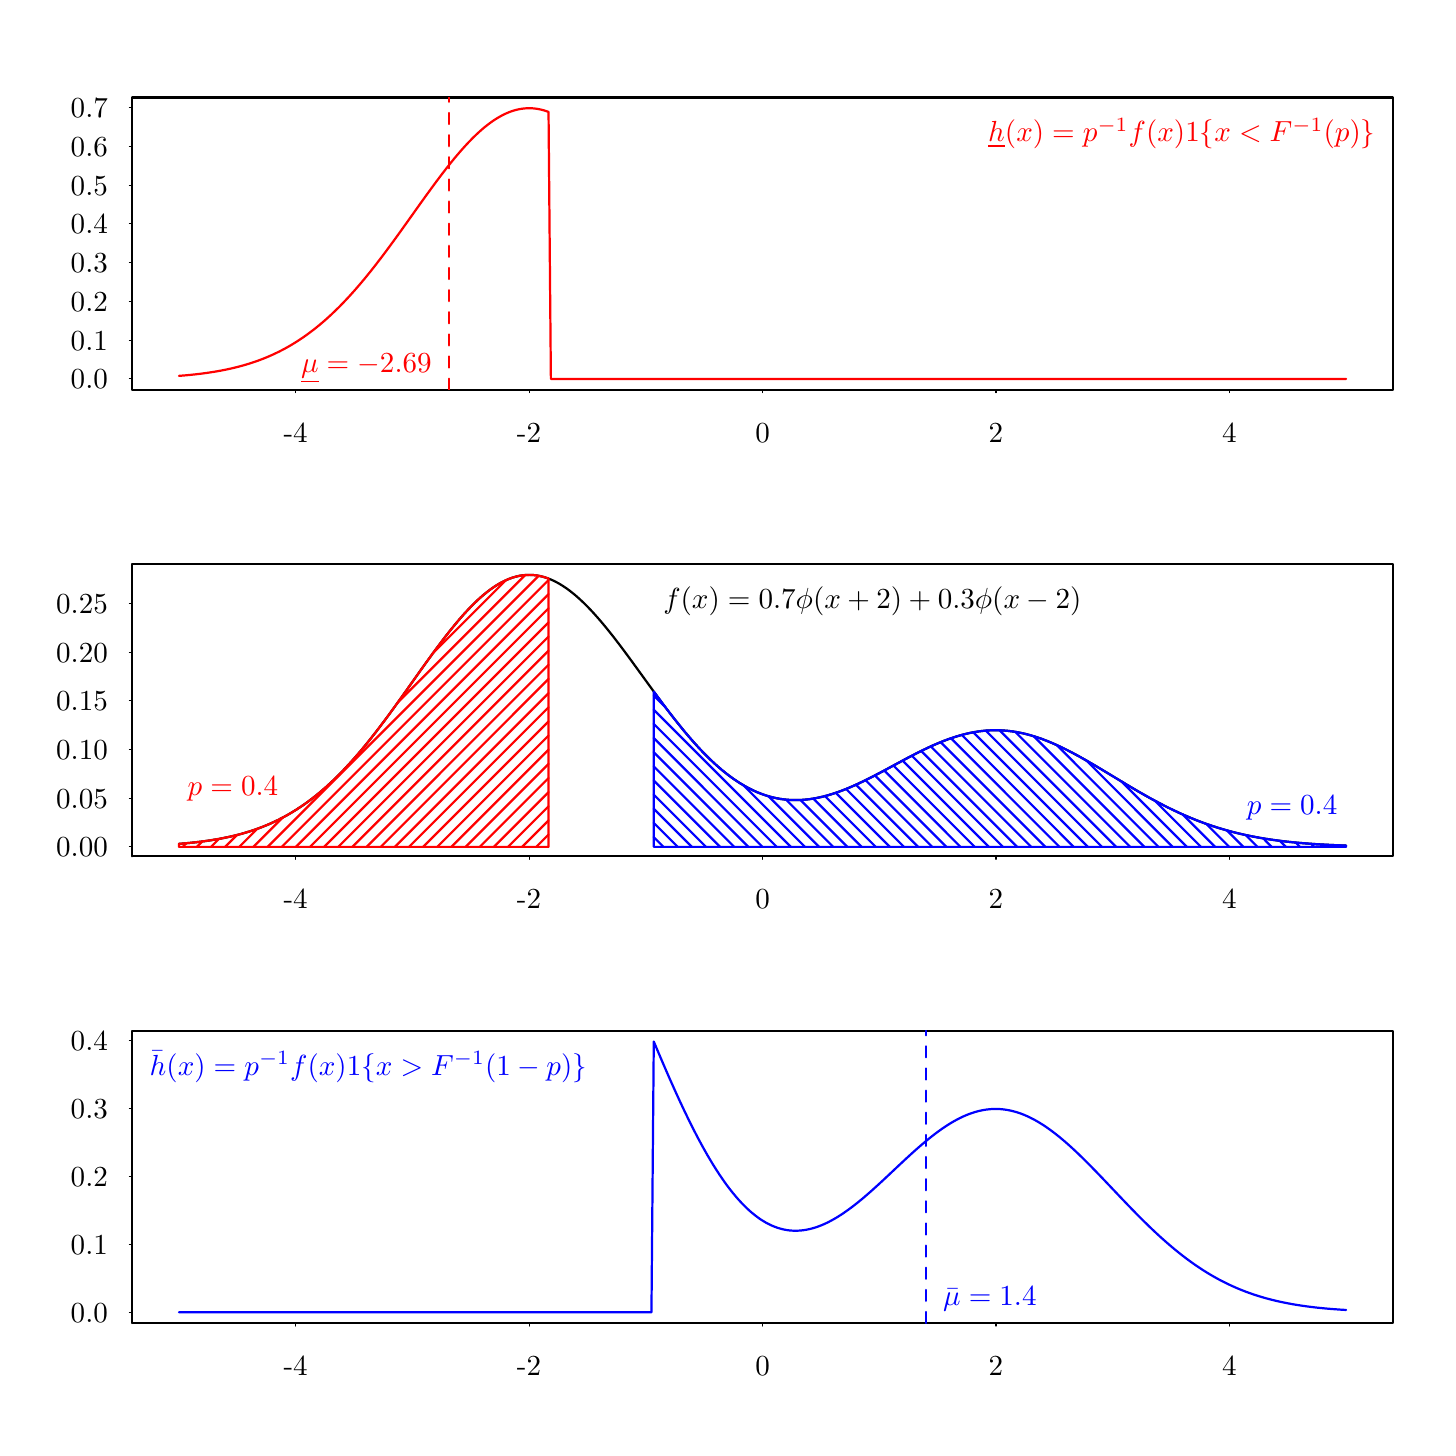
\begin{tikzpicture}[x=1pt,y=1pt]
\definecolor{fillColor}{RGB}{255,255,255}
\path[use as bounding box,fill=fillColor,fill opacity=0.00] (0,0) rectangle (505.89,505.89);
\begin{scope}
\path[clip] ( 37.80,375.06) rectangle (493.29,480.69);
\definecolor{drawColor}{RGB}{255,0,0}

\path[draw=drawColor,line width= 0.8pt,line join=round,line cap=round] ( 54.67,380.06) --
	( 55.52,380.13) --
	( 56.36,380.20) --
	( 57.21,380.27) --
	( 58.05,380.35) --
	( 58.90,380.43) --
	( 59.74,380.52) --
	( 60.59,380.61) --
	( 61.43,380.71) --
	( 62.28,380.81) --
	( 63.12,380.91) --
	( 63.97,381.03) --
	( 64.81,381.14) --
	( 65.66,381.27) --
	( 66.50,381.40) --
	( 67.35,381.53) --
	( 68.19,381.67) --
	( 69.04,381.82) --
	( 69.88,381.98) --
	( 70.73,382.14) --
	( 71.57,382.31) --
	( 72.42,382.49) --
	( 73.26,382.67) --
	( 74.11,382.87) --
	( 74.95,383.07) --
	( 75.80,383.28) --
	( 76.64,383.50) --
	( 77.49,383.73) --
	( 78.34,383.97) --
	( 79.18,384.22) --
	( 80.03,384.48) --
	( 80.87,384.75) --
	( 81.72,385.03) --
	( 82.56,385.32) --
	( 83.41,385.62) --
	( 84.25,385.94) --
	( 85.10,386.27) --
	( 85.94,386.60) --
	( 86.79,386.96) --
	( 87.63,387.32) --
	( 88.48,387.70) --
	( 89.32,388.09) --
	( 90.17,388.50) --
	( 91.01,388.91) --
	( 91.86,389.35) --
	( 92.70,389.79) --
	( 93.55,390.26) --
	( 94.39,390.73) --
	( 95.24,391.23) --
	( 96.08,391.74) --
	( 96.93,392.26) --
	( 97.77,392.80) --
	( 98.62,393.36) --
	( 99.47,393.93) --
	(100.31,394.52) --
	(101.16,395.12) --
	(102.00,395.75) --
	(102.85,396.39) --
	(103.69,397.04) --
	(104.54,397.72) --
	(105.38,398.41) --
	(106.23,399.12) --
	(107.07,399.84) --
	(107.92,400.59) --
	(108.76,401.35) --
	(109.61,402.13) --
	(110.45,402.93) --
	(111.30,403.74) --
	(112.14,404.57) --
	(112.99,405.42) --
	(113.83,406.28) --
	(114.68,407.17) --
	(115.52,408.07) --
	(116.37,408.98) --
	(117.21,409.92) --
	(118.06,410.86) --
	(118.90,411.83) --
	(119.75,412.81) --
	(120.59,413.80) --
	(121.44,414.82) --
	(122.29,415.84) --
	(123.13,416.88) --
	(123.98,417.93) --
	(124.82,419.00) --
	(125.67,420.08) --
	(126.51,421.17) --
	(127.36,422.27) --
	(128.20,423.38) --
	(129.05,424.50) --
	(129.89,425.64) --
	(130.74,426.78) --
	(131.58,427.93) --
	(132.43,429.09) --
	(133.27,430.25) --
	(134.12,431.42) --
	(134.96,432.60) --
	(135.81,433.78) --
	(136.65,434.96) --
	(137.50,436.15) --
	(138.34,437.34) --
	(139.19,438.52) --
	(140.03,439.71) --
	(140.88,440.90) --
	(141.72,442.09) --
	(142.57,443.27) --
	(143.41,444.45) --
	(144.26,445.62) --
	(145.11,446.78) --
	(145.95,447.94) --
	(146.80,449.09) --
	(147.64,450.24) --
	(148.49,451.37) --
	(149.33,452.49) --
	(150.18,453.59) --
	(151.02,454.68) --
	(151.87,455.76) --
	(152.71,456.82) --
	(153.56,457.87) --
	(154.40,458.90) --
	(155.25,459.90) --
	(156.09,460.89) --
	(156.94,461.86) --
	(157.78,462.80) --
	(158.63,463.72) --
	(159.47,464.62) --
	(160.32,465.49) --
	(161.16,466.34) --
	(162.01,467.15) --
	(162.85,467.94) --
	(163.70,468.71) --
	(164.54,469.44) --
	(165.39,470.14) --
	(166.24,470.81) --
	(167.08,471.44) --
	(167.93,472.05) --
	(168.77,472.62) --
	(169.62,473.15) --
	(170.46,473.65) --
	(171.31,474.12) --
	(172.15,474.55) --
	(173.00,474.94) --
	(173.84,475.30) --
	(174.69,475.62) --
	(175.53,475.90) --
	(176.38,476.14) --
	(177.22,476.34) --
	(178.07,476.51) --
	(178.91,476.63) --
	(179.76,476.72) --
	(180.60,476.77) --
	(181.45,476.78) --
	(182.29,476.75) --
	(183.14,476.68) --
	(183.98,476.57) --
	(184.83,476.42) --
	(185.67,476.24) --
	(186.52,476.01) --
	(187.36,475.75) --
	(188.21,475.45) --
	(189.06,378.97) --
	(189.90,378.97) --
	(190.75,378.97) --
	(191.59,378.97) --
	(192.44,378.97) --
	(193.28,378.97) --
	(194.13,378.97) --
	(194.97,378.97) --
	(195.82,378.97) --
	(196.66,378.97) --
	(197.51,378.97) --
	(198.35,378.97) --
	(199.20,378.97) --
	(200.04,378.97) --
	(200.89,378.97) --
	(201.73,378.97) --
	(202.58,378.97) --
	(203.42,378.97) --
	(204.27,378.97) --
	(205.11,378.97) --
	(205.96,378.97) --
	(206.80,378.97) --
	(207.65,378.97) --
	(208.49,378.97) --
	(209.34,378.97) --
	(210.19,378.97) --
	(211.03,378.97) --
	(211.88,378.97) --
	(212.72,378.97) --
	(213.57,378.97) --
	(214.41,378.97) --
	(215.26,378.97) --
	(216.10,378.97) --
	(216.95,378.97) --
	(217.79,378.97) --
	(218.64,378.97) --
	(219.48,378.97) --
	(220.33,378.97) --
	(221.17,378.97) --
	(222.02,378.97) --
	(222.86,378.97) --
	(223.71,378.97) --
	(224.55,378.97) --
	(225.40,378.97) --
	(226.24,378.97) --
	(227.09,378.97) --
	(227.93,378.97) --
	(228.78,378.97) --
	(229.62,378.97) --
	(230.47,378.97) --
	(231.31,378.97) --
	(232.16,378.97) --
	(233.01,378.97) --
	(233.85,378.97) --
	(234.70,378.97) --
	(235.54,378.97) --
	(236.39,378.97) --
	(237.23,378.97) --
	(238.08,378.97) --
	(238.92,378.97) --
	(239.77,378.97) --
	(240.61,378.97) --
	(241.46,378.97) --
	(242.30,378.97) --
	(243.15,378.97) --
	(243.99,378.97) --
	(244.84,378.97) --
	(245.68,378.97) --
	(246.53,378.97) --
	(247.37,378.97) --
	(248.22,378.97) --
	(249.06,378.97) --
	(249.91,378.97) --
	(250.75,378.97) --
	(251.60,378.97) --
	(252.44,378.97) --
	(253.29,378.97) --
	(254.13,378.97) --
	(254.98,378.97) --
	(255.83,378.97) --
	(256.67,378.97) --
	(257.52,378.97) --
	(258.36,378.97) --
	(259.21,378.97) --
	(260.05,378.97) --
	(260.90,378.97) --
	(261.74,378.97) --
	(262.59,378.97) --
	(263.43,378.97) --
	(264.28,378.97) --
	(265.12,378.97) --
	(265.97,378.97) --
	(266.81,378.97) --
	(267.66,378.97) --
	(268.50,378.97) --
	(269.35,378.97) --
	(270.19,378.97) --
	(271.04,378.97) --
	(271.88,378.97) --
	(272.73,378.97) --
	(273.57,378.97) --
	(274.42,378.97) --
	(275.26,378.97) --
	(276.11,378.97) --
	(276.96,378.97) --
	(277.80,378.97) --
	(278.65,378.97) --
	(279.49,378.97) --
	(280.34,378.97) --
	(281.18,378.97) --
	(282.03,378.97) --
	(282.87,378.97) --
	(283.72,378.97) --
	(284.56,378.97) --
	(285.41,378.97) --
	(286.25,378.97) --
	(287.10,378.97) --
	(287.94,378.97) --
	(288.79,378.97) --
	(289.63,378.97) --
	(290.48,378.97) --
	(291.32,378.97) --
	(292.17,378.97) --
	(293.01,378.97) --
	(293.86,378.97) --
	(294.70,378.97) --
	(295.55,378.97) --
	(296.39,378.97) --
	(297.24,378.97) --
	(298.08,378.97) --
	(298.93,378.97) --
	(299.78,378.97) --
	(300.62,378.97) --
	(301.47,378.97) --
	(302.31,378.97) --
	(303.16,378.97) --
	(304.00,378.97) --
	(304.85,378.97) --
	(305.69,378.97) --
	(306.54,378.97) --
	(307.38,378.97) --
	(308.23,378.97) --
	(309.07,378.97) --
	(309.92,378.97) --
	(310.76,378.97) --
	(311.61,378.97) --
	(312.45,378.97) --
	(313.30,378.97) --
	(314.14,378.97) --
	(314.99,378.97) --
	(315.83,378.97) --
	(316.68,378.97) --
	(317.52,378.97) --
	(318.37,378.97) --
	(319.21,378.97) --
	(320.06,378.97) --
	(320.90,378.97) --
	(321.75,378.97) --
	(322.60,378.97) --
	(323.44,378.97) --
	(324.29,378.97) --
	(325.13,378.97) --
	(325.98,378.97) --
	(326.82,378.97) --
	(327.67,378.97) --
	(328.51,378.97) --
	(329.36,378.97) --
	(330.20,378.97) --
	(331.05,378.97) --
	(331.89,378.97) --
	(332.74,378.97) --
	(333.58,378.97) --
	(334.43,378.97) --
	(335.27,378.97) --
	(336.12,378.97) --
	(336.96,378.97) --
	(337.81,378.97) --
	(338.65,378.97) --
	(339.50,378.97) --
	(340.34,378.97) --
	(341.19,378.97) --
	(342.03,378.97) --
	(342.88,378.97) --
	(343.73,378.97) --
	(344.57,378.97) --
	(345.42,378.97) --
	(346.26,378.97) --
	(347.11,378.97) --
	(347.95,378.97) --
	(348.80,378.97) --
	(349.64,378.97) --
	(350.49,378.97) --
	(351.33,378.97) --
	(352.18,378.97) --
	(353.02,378.97) --
	(353.87,378.97) --
	(354.71,378.97) --
	(355.56,378.97) --
	(356.40,378.97) --
	(357.25,378.97) --
	(358.09,378.97) --
	(358.94,378.97) --
	(359.78,378.97) --
	(360.63,378.97) --
	(361.47,378.97) --
	(362.32,378.97) --
	(363.16,378.97) --
	(364.01,378.97) --
	(364.85,378.97) --
	(365.70,378.97) --
	(366.55,378.97) --
	(367.39,378.97) --
	(368.24,378.97) --
	(369.08,378.97) --
	(369.93,378.97) --
	(370.77,378.97) --
	(371.62,378.97) --
	(372.46,378.97) --
	(373.31,378.97) --
	(374.15,378.97) --
	(375.00,378.97) --
	(375.84,378.97) --
	(376.69,378.97) --
	(377.53,378.97) --
	(378.38,378.97) --
	(379.22,378.97) --
	(380.07,378.97) --
	(380.91,378.97) --
	(381.76,378.97) --
	(382.60,378.97) --
	(383.45,378.97) --
	(384.29,378.97) --
	(385.14,378.97) --
	(385.98,378.97) --
	(386.83,378.97) --
	(387.68,378.97) --
	(388.52,378.97) --
	(389.37,378.97) --
	(390.21,378.97) --
	(391.06,378.97) --
	(391.90,378.97) --
	(392.75,378.97) --
	(393.59,378.97) --
	(394.44,378.97) --
	(395.28,378.97) --
	(396.13,378.97) --
	(396.97,378.97) --
	(397.82,378.97) --
	(398.66,378.97) --
	(399.51,378.97) --
	(400.35,378.97) --
	(401.20,378.97) --
	(402.04,378.97) --
	(402.89,378.97) --
	(403.73,378.97) --
	(404.58,378.97) --
	(405.42,378.97) --
	(406.27,378.97) --
	(407.11,378.97) --
	(407.96,378.97) --
	(408.80,378.97) --
	(409.65,378.97) --
	(410.50,378.97) --
	(411.34,378.97) --
	(412.19,378.97) --
	(413.03,378.97) --
	(413.88,378.97) --
	(414.72,378.97) --
	(415.57,378.97) --
	(416.41,378.97) --
	(417.26,378.97) --
	(418.10,378.97) --
	(418.95,378.97) --
	(419.79,378.97) --
	(420.64,378.97) --
	(421.48,378.97) --
	(422.33,378.97) --
	(423.17,378.97) --
	(424.02,378.97) --
	(424.86,378.97) --
	(425.71,378.97) --
	(426.55,378.97) --
	(427.40,378.97) --
	(428.24,378.97) --
	(429.09,378.97) --
	(429.93,378.97) --
	(430.78,378.97) --
	(431.62,378.97) --
	(432.47,378.97) --
	(433.32,378.97) --
	(434.16,378.97) --
	(435.01,378.97) --
	(435.85,378.97) --
	(436.70,378.97) --
	(437.54,378.97) --
	(438.39,378.97) --
	(439.23,378.97) --
	(440.08,378.97) --
	(440.92,378.97) --
	(441.77,378.97) --
	(442.61,378.97) --
	(443.46,378.97) --
	(444.30,378.97) --
	(445.15,378.97) --
	(445.99,378.97) --
	(446.84,378.97) --
	(447.68,378.97) --
	(448.53,378.97) --
	(449.37,378.97) --
	(450.22,378.97) --
	(451.06,378.97) --
	(451.91,378.97) --
	(452.75,378.97) --
	(453.60,378.97) --
	(454.45,378.97) --
	(455.29,378.97) --
	(456.14,378.97) --
	(456.98,378.97) --
	(457.83,378.97) --
	(458.67,378.97) --
	(459.52,378.97) --
	(460.36,378.97) --
	(461.21,378.97) --
	(462.05,378.97) --
	(462.90,378.97) --
	(463.74,378.97) --
	(464.59,378.97) --
	(465.43,378.97) --
	(466.28,378.97) --
	(467.12,378.97) --
	(467.97,378.97) --
	(468.81,378.97) --
	(469.66,378.97) --
	(470.50,378.97) --
	(471.35,378.97) --
	(472.19,378.97) --
	(473.04,378.97) --
	(473.88,378.97) --
	(474.73,378.97) --
	(475.57,378.97) --
	(476.42,378.97);
\end{scope}
\begin{scope}
\path[clip] (  0.00,  0.00) rectangle (505.89,505.89);
\definecolor{drawColor}{RGB}{0,0,0}

\path[draw=drawColor,line width= 0.4pt,line join=round,line cap=round] ( 96.84,375.06) -- (434.25,375.06);

\path[draw=drawColor,line width= 0.4pt,line join=round,line cap=round] ( 96.84,375.06) -- ( 96.84,374.00);

\path[draw=drawColor,line width= 0.4pt,line join=round,line cap=round] (181.19,375.06) -- (181.19,374.00);

\path[draw=drawColor,line width= 0.4pt,line join=round,line cap=round] (265.54,375.06) -- (265.54,374.00);

\path[draw=drawColor,line width= 0.4pt,line join=round,line cap=round] (349.89,375.06) -- (349.89,374.00);

\path[draw=drawColor,line width= 0.4pt,line join=round,line cap=round] (434.25,375.06) -- (434.25,374.00);

\node[text=drawColor,anchor=base,inner sep=0pt, outer sep=0pt, scale=  1.05] at ( 96.84,356.16) {-4};

\node[text=drawColor,anchor=base,inner sep=0pt, outer sep=0pt, scale=  1.05] at (181.19,356.16) {-2};

\node[text=drawColor,anchor=base,inner sep=0pt, outer sep=0pt, scale=  1.05] at (265.54,356.16) {0};

\node[text=drawColor,anchor=base,inner sep=0pt, outer sep=0pt, scale=  1.05] at (349.89,356.16) {2};

\node[text=drawColor,anchor=base,inner sep=0pt, outer sep=0pt, scale=  1.05] at (434.25,356.16) {4};

\path[draw=drawColor,line width= 0.4pt,line join=round,line cap=round] ( 37.80,378.97) -- ( 37.80,477.02);

\path[draw=drawColor,line width= 0.4pt,line join=round,line cap=round] ( 37.80,378.97) -- ( 36.74,378.97);

\path[draw=drawColor,line width= 0.4pt,line join=round,line cap=round] ( 37.80,392.98) -- ( 36.74,392.98);

\path[draw=drawColor,line width= 0.4pt,line join=round,line cap=round] ( 37.80,406.99) -- ( 36.74,406.99);

\path[draw=drawColor,line width= 0.4pt,line join=round,line cap=round] ( 37.80,420.99) -- ( 36.74,420.99);

\path[draw=drawColor,line width= 0.4pt,line join=round,line cap=round] ( 37.80,435.00) -- ( 36.74,435.00);

\path[draw=drawColor,line width= 0.4pt,line join=round,line cap=round] ( 37.80,449.01) -- ( 36.74,449.01);

\path[draw=drawColor,line width= 0.4pt,line join=round,line cap=round] ( 37.80,463.02) -- ( 36.74,463.02);

\path[draw=drawColor,line width= 0.4pt,line join=round,line cap=round] ( 37.80,477.02) -- ( 36.74,477.02);

\node[text=drawColor,anchor=base east,inner sep=0pt, outer sep=0pt, scale=  1.05] at ( 28.98,375.36) {0.0};

\node[text=drawColor,anchor=base east,inner sep=0pt, outer sep=0pt, scale=  1.05] at ( 28.98,389.36) {0.1};

\node[text=drawColor,anchor=base east,inner sep=0pt, outer sep=0pt, scale=  1.05] at ( 28.98,403.37) {0.2};

\node[text=drawColor,anchor=base east,inner sep=0pt, outer sep=0pt, scale=  1.05] at ( 28.98,417.38) {0.3};

\node[text=drawColor,anchor=base east,inner sep=0pt, outer sep=0pt, scale=  1.05] at ( 28.98,431.39) {0.4};

\node[text=drawColor,anchor=base east,inner sep=0pt, outer sep=0pt, scale=  1.05] at ( 28.98,445.39) {0.5};

\node[text=drawColor,anchor=base east,inner sep=0pt, outer sep=0pt, scale=  1.05] at ( 28.98,459.40) {0.6};

\node[text=drawColor,anchor=base east,inner sep=0pt, outer sep=0pt, scale=  1.05] at ( 28.98,473.41) {0.7};

\path[draw=drawColor,line width= 0.8pt,line join=round,line cap=round] ( 37.80,375.06) --
	(493.29,375.06) --
	(493.29,480.69) --
	( 37.80,480.69) --
	( 37.80,375.06);
\end{scope}
\begin{scope}
\path[clip] ( 37.80,375.06) rectangle (493.29,480.69);
\definecolor{drawColor}{RGB}{255,0,0}

\node[text=drawColor,anchor=base east,inner sep=0pt, outer sep=0pt, scale=  1.05] at (486.99,464.59) {$\underline{h}(x) = p^{-1}f(x) 1\{x < F^{-1}(p)\}$};

\path[draw=drawColor,line width= 0.8pt,dash pattern=on 4pt off 4pt ,line join=round,line cap=round] (152.27,375.06) -- (152.27,480.69);

\node[text=drawColor,anchor=base east,inner sep=0pt, outer sep=0pt, scale=  1.05] at (145.97,381.45) {$\underline{\mu} = -2.69$};
\end{scope}
\begin{scope}
\path[clip] ( 37.80,206.43) rectangle (493.29,312.06);
\definecolor{drawColor}{RGB}{0,0,0}

\path[draw=drawColor,line width= 0.8pt,line join=round,line cap=round] ( 54.67,210.97) --
	( 55.52,211.03) --
	( 56.36,211.10) --
	( 57.21,211.18) --
	( 58.05,211.26) --
	( 58.90,211.34) --
	( 59.74,211.43) --
	( 60.59,211.52) --
	( 61.43,211.62) --
	( 62.28,211.72) --
	( 63.12,211.83) --
	( 63.97,211.94) --
	( 64.81,212.06) --
	( 65.66,212.18) --
	( 66.50,212.31) --
	( 67.35,212.45) --
	( 68.19,212.59) --
	( 69.04,212.74) --
	( 69.88,212.89) --
	( 70.73,213.06) --
	( 71.57,213.23) --
	( 72.42,213.41) --
	( 73.26,213.59) --
	( 74.11,213.79) --
	( 74.95,213.99) --
	( 75.80,214.20) --
	( 76.64,214.42) --
	( 77.49,214.65) --
	( 78.34,214.90) --
	( 79.18,215.15) --
	( 80.03,215.41) --
	( 80.87,215.68) --
	( 81.72,215.96) --
	( 82.56,216.25) --
	( 83.41,216.56) --
	( 84.25,216.87) --
	( 85.10,217.20) --
	( 85.94,217.54) --
	( 86.79,217.90) --
	( 87.63,218.26) --
	( 88.48,218.64) --
	( 89.32,219.04) --
	( 90.17,219.44) --
	( 91.01,219.86) --
	( 91.86,220.30) --
	( 92.70,220.75) --
	( 93.55,221.21) --
	( 94.39,221.69) --
	( 95.24,222.19) --
	( 96.08,222.70) --
	( 96.93,223.23) --
	( 97.77,223.77) --
	( 98.62,224.33) --
	( 99.47,224.90) --
	(100.31,225.49) --
	(101.16,226.10) --
	(102.00,226.73) --
	(102.85,227.37) --
	(103.69,228.03) --
	(104.54,228.71) --
	(105.38,229.40) --
	(106.23,230.12) --
	(107.07,230.85) --
	(107.92,231.59) --
	(108.76,232.36) --
	(109.61,233.14) --
	(110.45,233.94) --
	(111.30,234.76) --
	(112.14,235.59) --
	(112.99,236.45) --
	(113.83,237.32) --
	(114.68,238.20) --
	(115.52,239.11) --
	(116.37,240.03) --
	(117.21,240.97) --
	(118.06,241.92) --
	(118.90,242.89) --
	(119.75,243.87) --
	(120.59,244.87) --
	(121.44,245.89) --
	(122.29,246.92) --
	(123.13,247.96) --
	(123.98,249.02) --
	(124.82,250.09) --
	(125.67,251.17) --
	(126.51,252.27) --
	(127.36,253.38) --
	(128.20,254.50) --
	(129.05,255.62) --
	(129.89,256.76) --
	(130.74,257.91) --
	(131.58,259.07) --
	(132.43,260.23) --
	(133.27,261.40) --
	(134.12,262.58) --
	(134.96,263.76) --
	(135.81,264.94) --
	(136.65,266.13) --
	(137.50,267.32) --
	(138.34,268.52) --
	(139.19,269.71) --
	(140.03,270.91) --
	(140.88,272.10) --
	(141.72,273.29) --
	(142.57,274.48) --
	(143.41,275.66) --
	(144.26,276.84) --
	(145.11,278.01) --
	(145.95,279.18) --
	(146.80,280.33) --
	(147.64,281.48) --
	(148.49,282.61) --
	(149.33,283.74) --
	(150.18,284.85) --
	(151.02,285.95) --
	(151.87,287.03) --
	(152.71,288.10) --
	(153.56,289.15) --
	(154.40,290.18) --
	(155.25,291.19) --
	(156.09,292.19) --
	(156.94,293.16) --
	(157.78,294.11) --
	(158.63,295.03) --
	(159.47,295.93) --
	(160.32,296.81) --
	(161.16,297.66) --
	(162.01,298.48) --
	(162.85,299.27) --
	(163.70,300.04) --
	(164.54,300.77) --
	(165.39,301.47) --
	(166.24,302.15) --
	(167.08,302.79) --
	(167.93,303.39) --
	(168.77,303.97) --
	(169.62,304.51) --
	(170.46,305.01) --
	(171.31,305.48) --
	(172.15,305.91) --
	(173.00,306.30) --
	(173.84,306.66) --
	(174.69,306.98) --
	(175.53,307.26) --
	(176.38,307.50) --
	(177.22,307.71) --
	(178.07,307.88) --
	(178.91,308.00) --
	(179.76,308.09) --
	(180.60,308.14) --
	(181.45,308.15) --
	(182.29,308.12) --
	(183.14,308.05) --
	(183.98,307.94) --
	(184.83,307.79) --
	(185.67,307.60) --
	(186.52,307.38) --
	(187.36,307.11) --
	(188.21,306.81) --
	(189.06,306.47) --
	(189.90,306.10) --
	(190.75,305.68) --
	(191.59,305.23) --
	(192.44,304.75) --
	(193.28,304.22) --
	(194.13,303.67) --
	(194.97,303.08) --
	(195.82,302.46) --
	(196.66,301.80) --
	(197.51,301.12) --
	(198.35,300.40) --
	(199.20,299.65) --
	(200.04,298.87) --
	(200.89,298.07) --
	(201.73,297.24) --
	(202.58,296.38) --
	(203.42,295.49) --
	(204.27,294.59) --
	(205.11,293.65) --
	(205.96,292.70) --
	(206.80,291.73) --
	(207.65,290.73) --
	(208.49,289.72) --
	(209.34,288.68) --
	(210.19,287.63) --
	(211.03,286.57) --
	(211.88,285.49) --
	(212.72,284.40) --
	(213.57,283.29) --
	(214.41,282.18) --
	(215.26,281.05) --
	(216.10,279.91) --
	(216.95,278.77) --
	(217.79,277.62) --
	(218.64,276.46) --
	(219.48,275.30) --
	(220.33,274.14) --
	(221.17,272.97) --
	(222.02,271.81) --
	(222.86,270.64) --
	(223.71,269.47) --
	(224.55,268.31) --
	(225.40,267.15) --
	(226.24,265.99) --
	(227.09,264.84) --
	(227.93,263.69) --
	(228.78,262.55) --
	(229.62,261.42) --
	(230.47,260.29) --
	(231.31,259.18) --
	(232.16,258.08) --
	(233.01,256.98) --
	(233.85,255.90) --
	(234.70,254.83) --
	(235.54,253.78) --
	(236.39,252.74) --
	(237.23,251.71) --
	(238.08,250.70) --
	(238.92,249.71) --
	(239.77,248.73) --
	(240.61,247.77) --
	(241.46,246.82) --
	(242.30,245.90) --
	(243.15,244.99) --
	(243.99,244.10) --
	(244.84,243.24) --
	(245.68,242.39) --
	(246.53,241.56) --
	(247.37,240.76) --
	(248.22,239.97) --
	(249.06,239.21) --
	(249.91,238.47) --
	(250.75,237.75) --
	(251.60,237.05) --
	(252.44,236.38) --
	(253.29,235.73) --
	(254.13,235.10) --
	(254.98,234.49) --
	(255.83,233.91) --
	(256.67,233.35) --
	(257.52,232.81) --
	(258.36,232.30) --
	(259.21,231.81) --
	(260.05,231.34) --
	(260.90,230.90) --
	(261.74,230.48) --
	(262.59,230.08) --
	(263.43,229.70) --
	(264.28,229.35) --
	(265.12,229.03) --
	(265.97,228.72) --
	(266.81,228.44) --
	(267.66,228.18) --
	(268.50,227.94) --
	(269.35,227.73) --
	(270.19,227.54) --
	(271.04,227.37) --
	(271.88,227.22) --
	(272.73,227.09) --
	(273.57,226.99) --
	(274.42,226.90) --
	(275.26,226.84) --
	(276.11,226.80) --
	(276.96,226.78) --
	(277.80,226.77) --
	(278.65,226.79) --
	(279.49,226.83) --
	(280.34,226.88) --
	(281.18,226.96) --
	(282.03,227.05) --
	(282.87,227.16) --
	(283.72,227.29) --
	(284.56,227.44) --
	(285.41,227.60) --
	(286.25,227.78) --
	(287.10,227.97) --
	(287.94,228.18) --
	(288.79,228.41) --
	(289.63,228.65) --
	(290.48,228.91) --
	(291.32,229.18) --
	(292.17,229.46) --
	(293.01,229.76) --
	(293.86,230.07) --
	(294.70,230.39) --
	(295.55,230.72) --
	(296.39,231.07) --
	(297.24,231.42) --
	(298.08,231.79) --
	(298.93,232.16) --
	(299.78,232.55) --
	(300.62,232.94) --
	(301.47,233.34) --
	(302.31,233.75) --
	(303.16,234.16) --
	(304.00,234.59) --
	(304.85,235.01) --
	(305.69,235.45) --
	(306.54,235.89) --
	(307.38,236.33) --
	(308.23,236.78) --
	(309.07,237.23) --
	(309.92,237.68) --
	(310.76,238.13) --
	(311.61,238.59) --
	(312.45,239.05) --
	(313.30,239.50) --
	(314.14,239.96) --
	(314.99,240.41) --
	(315.83,240.87) --
	(316.68,241.32) --
	(317.52,241.77) --
	(318.37,242.22) --
	(319.21,242.66) --
	(320.06,243.10) --
	(320.90,243.53) --
	(321.75,243.96) --
	(322.60,244.38) --
	(323.44,244.80) --
	(324.29,245.21) --
	(325.13,245.61) --
	(325.98,246.00) --
	(326.82,246.39) --
	(327.67,246.76) --
	(328.51,247.13) --
	(329.36,247.48) --
	(330.20,247.83) --
	(331.05,248.16) --
	(331.89,248.49) --
	(332.74,248.80) --
	(333.58,249.09) --
	(334.43,249.38) --
	(335.27,249.65) --
	(336.12,249.91) --
	(336.96,250.16) --
	(337.81,250.39) --
	(338.65,250.61) --
	(339.50,250.81) --
	(340.34,251.00) --
	(341.19,251.17) --
	(342.03,251.33) --
	(342.88,251.47) --
	(343.73,251.60) --
	(344.57,251.71) --
	(345.42,251.80) --
	(346.26,251.88) --
	(347.11,251.94) --
	(347.95,251.98) --
	(348.80,252.01) --
	(349.64,252.02) --
	(350.49,252.01) --
	(351.33,251.99) --
	(352.18,251.95) --
	(353.02,251.89) --
	(353.87,251.82) --
	(354.71,251.73) --
	(355.56,251.63) --
	(356.40,251.51) --
	(357.25,251.37) --
	(358.09,251.21) --
	(358.94,251.04) --
	(359.78,250.86) --
	(360.63,250.66) --
	(361.47,250.44) --
	(362.32,250.21) --
	(363.16,249.96) --
	(364.01,249.70) --
	(364.85,249.43) --
	(365.70,249.14) --
	(366.55,248.84) --
	(367.39,248.52) --
	(368.24,248.19) --
	(369.08,247.85) --
	(369.93,247.50) --
	(370.77,247.13) --
	(371.62,246.76) --
	(372.46,246.37) --
	(373.31,245.98) --
	(374.15,245.57) --
	(375.00,245.15) --
	(375.84,244.73) --
	(376.69,244.29) --
	(377.53,243.85) --
	(378.38,243.40) --
	(379.22,242.94) --
	(380.07,242.48) --
	(380.91,242.01) --
	(381.76,241.53) --
	(382.60,241.05) --
	(383.45,240.56) --
	(384.29,240.07) --
	(385.14,239.58) --
	(385.98,239.08) --
	(386.83,238.57) --
	(387.68,238.07) --
	(388.52,237.56) --
	(389.37,237.05) --
	(390.21,236.54) --
	(391.06,236.03) --
	(391.90,235.52) --
	(392.75,235.01) --
	(393.59,234.50) --
	(394.44,233.98) --
	(395.28,233.48) --
	(396.13,232.97) --
	(396.97,232.46) --
	(397.82,231.96) --
	(398.66,231.46) --
	(399.51,230.96) --
	(400.35,230.46) --
	(401.20,229.97) --
	(402.04,229.48) --
	(402.89,229.00) --
	(403.73,228.52) --
	(404.58,228.04) --
	(405.42,227.57) --
	(406.27,227.11) --
	(407.11,226.65) --
	(407.96,226.20) --
	(408.80,225.75) --
	(409.65,225.31) --
	(410.50,224.87) --
	(411.34,224.45) --
	(412.19,224.02) --
	(413.03,223.61) --
	(413.88,223.20) --
	(414.72,222.80) --
	(415.57,222.40) --
	(416.41,222.02) --
	(417.26,221.64) --
	(418.10,221.26) --
	(418.95,220.90) --
	(419.79,220.54) --
	(420.64,220.19) --
	(421.48,219.85) --
	(422.33,219.51) --
	(423.17,219.18) --
	(424.02,218.86) --
	(424.86,218.55) --
	(425.71,218.24) --
	(426.55,217.95) --
	(427.40,217.66) --
	(428.24,217.37) --
	(429.09,217.10) --
	(429.93,216.83) --
	(430.78,216.57) --
	(431.62,216.32) --
	(432.47,216.07) --
	(433.32,215.83) --
	(434.16,215.60) --
	(435.01,215.37) --
	(435.85,215.15) --
	(436.70,214.94) --
	(437.54,214.73) --
	(438.39,214.53) --
	(439.23,214.34) --
	(440.08,214.16) --
	(440.92,213.98) --
	(441.77,213.80) --
	(442.61,213.63) --
	(443.46,213.47) --
	(444.30,213.31) --
	(445.15,213.16) --
	(445.99,213.02) --
	(446.84,212.87) --
	(447.68,212.74) --
	(448.53,212.61) --
	(449.37,212.48) --
	(450.22,212.36) --
	(451.06,212.25) --
	(451.91,212.13) --
	(452.75,212.03) --
	(453.60,211.92) --
	(454.45,211.82) --
	(455.29,211.73) --
	(456.14,211.64) --
	(456.98,211.55) --
	(457.83,211.47) --
	(458.67,211.39) --
	(459.52,211.31) --
	(460.36,211.24) --
	(461.21,211.17) --
	(462.05,211.10) --
	(462.90,211.04) --
	(463.74,210.98) --
	(464.59,210.92) --
	(465.43,210.86) --
	(466.28,210.81) --
	(467.12,210.76) --
	(467.97,210.71) --
	(468.81,210.67) --
	(469.66,210.62) --
	(470.50,210.58) --
	(471.35,210.54) --
	(472.19,210.50) --
	(473.04,210.47) --
	(473.88,210.43) --
	(474.73,210.40) --
	(475.57,210.37) --
	(476.42,210.34);
\end{scope}
\begin{scope}
\path[clip] (  0.00,  0.00) rectangle (505.89,505.89);
\definecolor{drawColor}{RGB}{0,0,0}

\path[draw=drawColor,line width= 0.4pt,line join=round,line cap=round] ( 96.84,206.43) -- (434.25,206.43);

\path[draw=drawColor,line width= 0.4pt,line join=round,line cap=round] ( 96.84,206.43) -- ( 96.84,205.37);

\path[draw=drawColor,line width= 0.4pt,line join=round,line cap=round] (181.19,206.43) -- (181.19,205.37);

\path[draw=drawColor,line width= 0.4pt,line join=round,line cap=round] (265.54,206.43) -- (265.54,205.37);

\path[draw=drawColor,line width= 0.4pt,line join=round,line cap=round] (349.89,206.43) -- (349.89,205.37);

\path[draw=drawColor,line width= 0.4pt,line join=round,line cap=round] (434.25,206.43) -- (434.25,205.37);

\node[text=drawColor,anchor=base,inner sep=0pt, outer sep=0pt, scale=  1.05] at ( 96.84,187.53) {-4};

\node[text=drawColor,anchor=base,inner sep=0pt, outer sep=0pt, scale=  1.05] at (181.19,187.53) {-2};

\node[text=drawColor,anchor=base,inner sep=0pt, outer sep=0pt, scale=  1.05] at (265.54,187.53) {0};

\node[text=drawColor,anchor=base,inner sep=0pt, outer sep=0pt, scale=  1.05] at (349.89,187.53) {2};

\node[text=drawColor,anchor=base,inner sep=0pt, outer sep=0pt, scale=  1.05] at (434.25,187.53) {4};

\path[draw=drawColor,line width= 0.4pt,line join=round,line cap=round] ( 37.80,209.87) -- ( 37.80,297.84);

\path[draw=drawColor,line width= 0.4pt,line join=round,line cap=round] ( 37.80,209.87) -- ( 36.74,209.87);

\path[draw=drawColor,line width= 0.4pt,line join=round,line cap=round] ( 37.80,227.47) -- ( 36.74,227.47);

\path[draw=drawColor,line width= 0.4pt,line join=round,line cap=round] ( 37.80,245.06) -- ( 36.74,245.06);

\path[draw=drawColor,line width= 0.4pt,line join=round,line cap=round] ( 37.80,262.65) -- ( 36.74,262.65);

\path[draw=drawColor,line width= 0.4pt,line join=round,line cap=round] ( 37.80,280.25) -- ( 36.74,280.25);

\path[draw=drawColor,line width= 0.4pt,line join=round,line cap=round] ( 37.80,297.84) -- ( 36.74,297.84);

\node[text=drawColor,anchor=base east,inner sep=0pt, outer sep=0pt, scale=  1.05] at ( 28.98,206.26) {0.00};

\node[text=drawColor,anchor=base east,inner sep=0pt, outer sep=0pt, scale=  1.05] at ( 28.98,223.85) {0.05};

\node[text=drawColor,anchor=base east,inner sep=0pt, outer sep=0pt, scale=  1.05] at ( 28.98,241.44) {0.10};

\node[text=drawColor,anchor=base east,inner sep=0pt, outer sep=0pt, scale=  1.05] at ( 28.98,259.04) {0.15};

\node[text=drawColor,anchor=base east,inner sep=0pt, outer sep=0pt, scale=  1.05] at ( 28.98,276.63) {0.20};

\node[text=drawColor,anchor=base east,inner sep=0pt, outer sep=0pt, scale=  1.05] at ( 28.98,294.22) {0.25};

\path[draw=drawColor,line width= 0.8pt,line join=round,line cap=round] ( 37.80,206.43) --
	(493.29,206.43) --
	(493.29,312.06) --
	( 37.80,312.06) --
	( 37.80,206.43);
\end{scope}
\begin{scope}
\path[clip] ( 37.80,206.43) rectangle (493.29,312.06);
\definecolor{drawColor}{RGB}{255,0,0}

\path[draw=drawColor,line width= 0.8pt,line join=round,line cap=round] ( 56.02,209.87) -- ( 57.34,211.19);

\path[draw=drawColor,line width= 0.8pt,line join=round,line cap=round] ( 61.13,209.87) -- ( 63.08,211.82);

\path[draw=drawColor,line width= 0.8pt,line join=round,line cap=round] ( 66.24,209.87) -- ( 69.12,212.75);

\path[draw=drawColor,line width= 0.8pt,line join=round,line cap=round] ( 71.36,209.87) -- ( 75.64,214.16);

\path[draw=drawColor,line width= 0.8pt,line join=round,line cap=round] ( 76.47,209.87) -- ( 83.00,216.41);

\path[draw=drawColor,line width= 0.8pt,line join=round,line cap=round] (146.45,279.86) -- (172.80,306.21);

\path[draw=drawColor,line width= 0.8pt,line join=round,line cap=round] ( 81.58,209.87) -- ( 92.16,220.46);

\path[draw=drawColor,line width= 0.8pt,line join=round,line cap=round] (133.71,262.01) -- (179.79,308.09);

\path[draw=drawColor,line width= 0.8pt,line join=round,line cap=round] ( 86.69,209.87) -- (184.64,307.82);

\path[draw=drawColor,line width= 0.8pt,line join=round,line cap=round] ( 91.80,209.87) -- (188.21,306.29);

\path[draw=drawColor,line width= 0.8pt,line join=round,line cap=round] ( 96.91,209.87) -- (188.21,301.18);

\path[draw=drawColor,line width= 0.8pt,line join=round,line cap=round] (102.02,209.87) -- (188.21,296.07);

\path[draw=drawColor,line width= 0.8pt,line join=round,line cap=round] (107.13,209.87) -- (188.21,290.96);

\path[draw=drawColor,line width= 0.8pt,line join=round,line cap=round] (112.24,209.87) -- (188.21,285.85);

\path[draw=drawColor,line width= 0.8pt,line join=round,line cap=round] (117.35,209.87) -- (188.21,280.74);

\path[draw=drawColor,line width= 0.8pt,line join=round,line cap=round] (122.46,209.87) -- (188.21,275.63);

\path[draw=drawColor,line width= 0.8pt,line join=round,line cap=round] (127.57,209.87) -- (188.21,270.52);

\path[draw=drawColor,line width= 0.8pt,line join=round,line cap=round] (132.68,209.87) -- (188.21,265.41);

\path[draw=drawColor,line width= 0.8pt,line join=round,line cap=round] (137.79,209.87) -- (188.21,260.30);

\path[draw=drawColor,line width= 0.8pt,line join=round,line cap=round] (142.90,209.87) -- (188.21,255.19);

\path[draw=drawColor,line width= 0.8pt,line join=round,line cap=round] (148.01,209.87) -- (188.21,250.08);

\path[draw=drawColor,line width= 0.8pt,line join=round,line cap=round] (153.12,209.87) -- (188.21,244.97);

\path[draw=drawColor,line width= 0.8pt,line join=round,line cap=round] (158.23,209.87) -- (188.21,239.85);

\path[draw=drawColor,line width= 0.8pt,line join=round,line cap=round] (163.34,209.87) -- (188.21,234.74);

\path[draw=drawColor,line width= 0.8pt,line join=round,line cap=round] (168.45,209.87) -- (188.21,229.63);

\path[draw=drawColor,line width= 0.8pt,line join=round,line cap=round] (173.56,209.87) -- (188.21,224.52);

\path[draw=drawColor,line width= 0.8pt,line join=round,line cap=round] (178.67,209.87) -- (188.21,219.41);

\path[draw=drawColor,line width= 0.8pt,line join=round,line cap=round] (183.78,209.87) -- (188.21,214.30);

\path[draw=drawColor,line width= 0.8pt,line join=round,line cap=round] ( 54.67,209.87) --
	( 55.52,209.87) --
	( 56.36,209.87) --
	( 57.21,209.87) --
	( 58.05,209.87) --
	( 58.90,209.87) --
	( 59.74,209.87) --
	( 60.59,209.87) --
	( 61.43,209.87) --
	( 62.28,209.87) --
	( 63.12,209.87) --
	( 63.97,209.87) --
	( 64.81,209.87) --
	( 65.66,209.87) --
	( 66.50,209.87) --
	( 67.35,209.87) --
	( 68.19,209.87) --
	( 69.04,209.87) --
	( 69.88,209.87) --
	( 70.73,209.87) --
	( 71.57,209.87) --
	( 72.42,209.87) --
	( 73.26,209.87) --
	( 74.11,209.87) --
	( 74.95,209.87) --
	( 75.80,209.87) --
	( 76.64,209.87) --
	( 77.49,209.87) --
	( 78.34,209.87) --
	( 79.18,209.87) --
	( 80.03,209.87) --
	( 80.87,209.87) --
	( 81.72,209.87) --
	( 82.56,209.87) --
	( 83.41,209.87) --
	( 84.25,209.87) --
	( 85.10,209.87) --
	( 85.94,209.87) --
	( 86.79,209.87) --
	( 87.63,209.87) --
	( 88.48,209.87) --
	( 89.32,209.87) --
	( 90.17,209.87) --
	( 91.01,209.87) --
	( 91.86,209.87) --
	( 92.70,209.87) --
	( 93.55,209.87) --
	( 94.39,209.87) --
	( 95.24,209.87) --
	( 96.08,209.87) --
	( 96.93,209.87) --
	( 97.77,209.87) --
	( 98.62,209.87) --
	( 99.47,209.87) --
	(100.31,209.87) --
	(101.16,209.87) --
	(102.00,209.87) --
	(102.85,209.87) --
	(103.69,209.87) --
	(104.54,209.87) --
	(105.38,209.87) --
	(106.23,209.87) --
	(107.07,209.87) --
	(107.92,209.87) --
	(108.76,209.87) --
	(109.61,209.87) --
	(110.45,209.87) --
	(111.30,209.87) --
	(112.14,209.87) --
	(112.99,209.87) --
	(113.83,209.87) --
	(114.68,209.87) --
	(115.52,209.87) --
	(116.37,209.87) --
	(117.21,209.87) --
	(118.06,209.87) --
	(118.90,209.87) --
	(119.75,209.87) --
	(120.59,209.87) --
	(121.44,209.87) --
	(122.29,209.87) --
	(123.13,209.87) --
	(123.98,209.87) --
	(124.82,209.87) --
	(125.67,209.87) --
	(126.51,209.87) --
	(127.36,209.87) --
	(128.20,209.87) --
	(129.05,209.87) --
	(129.89,209.87) --
	(130.74,209.87) --
	(131.58,209.87) --
	(132.43,209.87) --
	(133.27,209.87) --
	(134.12,209.87) --
	(134.96,209.87) --
	(135.81,209.87) --
	(136.65,209.87) --
	(137.50,209.87) --
	(138.34,209.87) --
	(139.19,209.87) --
	(140.03,209.87) --
	(140.88,209.87) --
	(141.72,209.87) --
	(142.57,209.87) --
	(143.41,209.87) --
	(144.26,209.87) --
	(145.11,209.87) --
	(145.95,209.87) --
	(146.80,209.87) --
	(147.64,209.87) --
	(148.49,209.87) --
	(149.33,209.87) --
	(150.18,209.87) --
	(151.02,209.87) --
	(151.87,209.87) --
	(152.71,209.87) --
	(153.56,209.87) --
	(154.40,209.87) --
	(155.25,209.87) --
	(156.09,209.87) --
	(156.94,209.87) --
	(157.78,209.87) --
	(158.63,209.87) --
	(159.47,209.87) --
	(160.32,209.87) --
	(161.16,209.87) --
	(162.01,209.87) --
	(162.85,209.87) --
	(163.70,209.87) --
	(164.54,209.87) --
	(165.39,209.87) --
	(166.24,209.87) --
	(167.08,209.87) --
	(167.93,209.87) --
	(168.77,209.87) --
	(169.62,209.87) --
	(170.46,209.87) --
	(171.31,209.87) --
	(172.15,209.87) --
	(173.00,209.87) --
	(173.84,209.87) --
	(174.69,209.87) --
	(175.53,209.87) --
	(176.38,209.87) --
	(177.22,209.87) --
	(178.07,209.87) --
	(178.91,209.87) --
	(179.76,209.87) --
	(180.60,209.87) --
	(181.45,209.87) --
	(182.29,209.87) --
	(183.14,209.87) --
	(183.98,209.87) --
	(184.83,209.87) --
	(185.67,209.87) --
	(186.52,209.87) --
	(187.36,209.87) --
	(188.21,209.87) --
	(188.21,306.81) --
	(187.36,307.11) --
	(186.52,307.38) --
	(185.67,307.60) --
	(184.83,307.79) --
	(183.98,307.94) --
	(183.14,308.05) --
	(182.29,308.12) --
	(181.45,308.15) --
	(180.60,308.14) --
	(179.76,308.09) --
	(178.91,308.00) --
	(178.07,307.88) --
	(177.22,307.71) --
	(176.38,307.50) --
	(175.53,307.26) --
	(174.69,306.98) --
	(173.84,306.66) --
	(173.00,306.30) --
	(172.15,305.91) --
	(171.31,305.48) --
	(170.46,305.01) --
	(169.62,304.51) --
	(168.77,303.97) --
	(167.93,303.39) --
	(167.08,302.79) --
	(166.24,302.15) --
	(165.39,301.47) --
	(164.54,300.77) --
	(163.70,300.04) --
	(162.85,299.27) --
	(162.01,298.48) --
	(161.16,297.66) --
	(160.32,296.81) --
	(159.47,295.93) --
	(158.63,295.03) --
	(157.78,294.11) --
	(156.94,293.16) --
	(156.09,292.19) --
	(155.25,291.19) --
	(154.40,290.18) --
	(153.56,289.15) --
	(152.71,288.10) --
	(151.87,287.03) --
	(151.02,285.95) --
	(150.18,284.85) --
	(149.33,283.74) --
	(148.49,282.61) --
	(147.64,281.48) --
	(146.80,280.33) --
	(145.95,279.18) --
	(145.11,278.01) --
	(144.26,276.84) --
	(143.41,275.66) --
	(142.57,274.48) --
	(141.72,273.29) --
	(140.88,272.10) --
	(140.03,270.91) --
	(139.19,269.71) --
	(138.34,268.52) --
	(137.50,267.32) --
	(136.65,266.13) --
	(135.81,264.94) --
	(134.96,263.76) --
	(134.12,262.58) --
	(133.27,261.40) --
	(132.43,260.23) --
	(131.58,259.07) --
	(130.74,257.91) --
	(129.89,256.76) --
	(129.05,255.62) --
	(128.20,254.50) --
	(127.36,253.38) --
	(126.51,252.27) --
	(125.67,251.17) --
	(124.82,250.09) --
	(123.98,249.02) --
	(123.13,247.96) --
	(122.29,246.92) --
	(121.44,245.89) --
	(120.59,244.87) --
	(119.75,243.87) --
	(118.90,242.89) --
	(118.06,241.92) --
	(117.21,240.97) --
	(116.37,240.03) --
	(115.52,239.11) --
	(114.68,238.20) --
	(113.83,237.32) --
	(112.99,236.45) --
	(112.14,235.59) --
	(111.30,234.76) --
	(110.45,233.94) --
	(109.61,233.14) --
	(108.76,232.36) --
	(107.92,231.59) --
	(107.07,230.85) --
	(106.23,230.12) --
	(105.38,229.40) --
	(104.54,228.71) --
	(103.69,228.03) --
	(102.85,227.37) --
	(102.00,226.73) --
	(101.16,226.10) --
	(100.31,225.49) --
	( 99.47,224.90) --
	( 98.62,224.33) --
	( 97.77,223.77) --
	( 96.93,223.23) --
	( 96.08,222.70) --
	( 95.24,222.19) --
	( 94.39,221.69) --
	( 93.55,221.21) --
	( 92.70,220.75) --
	( 91.86,220.30) --
	( 91.01,219.86) --
	( 90.17,219.44) --
	( 89.32,219.04) --
	( 88.48,218.64) --
	( 87.63,218.26) --
	( 86.79,217.90) --
	( 85.94,217.54) --
	( 85.10,217.20) --
	( 84.25,216.87) --
	( 83.41,216.56) --
	( 82.56,216.25) --
	( 81.72,215.96) --
	( 80.87,215.68) --
	( 80.03,215.41) --
	( 79.18,215.15) --
	( 78.34,214.90) --
	( 77.49,214.65) --
	( 76.64,214.42) --
	( 75.80,214.20) --
	( 74.95,213.99) --
	( 74.11,213.79) --
	( 73.26,213.59) --
	( 72.42,213.41) --
	( 71.57,213.23) --
	( 70.73,213.06) --
	( 69.88,212.89) --
	( 69.04,212.74) --
	( 68.19,212.59) --
	( 67.35,212.45) --
	( 66.50,212.31) --
	( 65.66,212.18) --
	( 64.81,212.06) --
	( 63.97,211.94) --
	( 63.12,211.83) --
	( 62.28,211.72) --
	( 61.43,211.62) --
	( 60.59,211.52) --
	( 59.74,211.43) --
	( 58.90,211.34) --
	( 58.05,211.26) --
	( 57.21,211.18) --
	( 56.36,211.10) --
	( 55.52,211.03) --
	( 54.67,210.97) --
	( 54.67,209.87);

\node[text=drawColor,anchor=base east,inner sep=0pt, outer sep=0pt, scale=  1.05] at ( 90.54,228.58) {$p = 0.4$};
\definecolor{drawColor}{RGB}{0,0,255}

\path[draw=drawColor,line width= 0.8pt,line join=round,line cap=round] (229.77,209.87) -- (226.24,213.40);

\path[draw=drawColor,line width= 0.8pt,line join=round,line cap=round] (234.88,209.87) -- (226.24,218.51);

\path[draw=drawColor,line width= 0.8pt,line join=round,line cap=round] (239.99,209.87) -- (226.24,223.62);

\path[draw=drawColor,line width= 0.8pt,line join=round,line cap=round] (245.10,209.87) -- (226.24,228.73);

\path[draw=drawColor,line width= 0.8pt,line join=round,line cap=round] (250.21,209.87) -- (226.24,233.84);

\path[draw=drawColor,line width= 0.8pt,line join=round,line cap=round] (255.32,209.87) -- (226.24,238.96);

\path[draw=drawColor,line width= 0.8pt,line join=round,line cap=round] (260.43,209.87) -- (226.24,244.07);

\path[draw=drawColor,line width= 0.8pt,line join=round,line cap=round] (265.54,209.87) -- (226.24,249.18);

\path[draw=drawColor,line width= 0.8pt,line join=round,line cap=round] (270.66,209.87) -- (226.24,254.29);

\path[draw=drawColor,line width= 0.8pt,line join=round,line cap=round] (275.77,209.87) -- (226.24,259.40);

\path[draw=drawColor,line width= 0.8pt,line join=round,line cap=round] (280.88,209.87) -- (258.58,232.17);

\path[draw=drawColor,line width= 0.8pt,line join=round,line cap=round] (230.51,260.24) -- (226.24,264.51);

\path[draw=drawColor,line width= 0.8pt,line join=round,line cap=round] (285.99,209.87) -- (267.69,228.17);

\path[draw=drawColor,line width= 0.8pt,line join=round,line cap=round] (291.10,209.87) -- (274.03,226.94);

\path[draw=drawColor,line width= 0.8pt,line join=round,line cap=round] (296.21,209.87) -- (279.26,226.82);

\path[draw=drawColor,line width= 0.8pt,line join=round,line cap=round] (301.32,209.87) -- (283.87,227.32);

\path[draw=drawColor,line width= 0.8pt,line join=round,line cap=round] (306.43,209.87) -- (288.08,228.22);

\path[draw=drawColor,line width= 0.8pt,line join=round,line cap=round] (311.54,209.87) -- (292.01,229.41);

\path[draw=drawColor,line width= 0.8pt,line join=round,line cap=round] (316.65,209.87) -- (295.73,230.79);

\path[draw=drawColor,line width= 0.8pt,line join=round,line cap=round] (321.76,209.87) -- (299.30,232.33);

\path[draw=drawColor,line width= 0.8pt,line join=round,line cap=round] (326.87,209.87) -- (302.77,233.97);

\path[draw=drawColor,line width= 0.8pt,line join=round,line cap=round] (331.98,209.87) -- (306.16,235.69);

\path[draw=drawColor,line width= 0.8pt,line join=round,line cap=round] (337.09,209.87) -- (309.51,237.46);

\path[draw=drawColor,line width= 0.8pt,line join=round,line cap=round] (342.20,209.87) -- (312.83,239.25);

\path[draw=drawColor,line width= 0.8pt,line join=round,line cap=round] (347.31,209.87) -- (316.15,241.04);

\path[draw=drawColor,line width= 0.8pt,line join=round,line cap=round] (352.42,209.87) -- (319.49,242.80);

\path[draw=drawColor,line width= 0.8pt,line join=round,line cap=round] (357.53,209.87) -- (322.88,244.52);

\path[draw=drawColor,line width= 0.8pt,line join=round,line cap=round] (362.64,209.87) -- (326.35,246.17);

\path[draw=drawColor,line width= 0.8pt,line join=round,line cap=round] (367.75,209.87) -- (329.91,247.71);

\path[draw=drawColor,line width= 0.8pt,line join=round,line cap=round] (372.86,209.87) -- (333.63,249.11);

\path[draw=drawColor,line width= 0.8pt,line join=round,line cap=round] (377.97,209.87) -- (337.53,250.32);

\path[draw=drawColor,line width= 0.8pt,line join=round,line cap=round] (383.08,209.87) -- (341.69,251.27);

\path[draw=drawColor,line width= 0.8pt,line join=round,line cap=round] (388.19,209.87) -- (346.20,251.87);

\path[draw=drawColor,line width= 0.8pt,line join=round,line cap=round] (393.30,209.87) -- (351.18,251.99);

\path[draw=drawColor,line width= 0.8pt,line join=round,line cap=round] (398.41,209.87) -- (356.85,251.43);

\path[draw=drawColor,line width= 0.8pt,line join=round,line cap=round] (403.52,209.87) -- (363.56,249.84);

\path[draw=drawColor,line width= 0.8pt,line join=round,line cap=round] (408.63,209.87) -- (371.86,246.65);

\path[draw=drawColor,line width= 0.8pt,line join=round,line cap=round] (413.74,209.87) -- (382.52,241.10);

\path[draw=drawColor,line width= 0.8pt,line join=round,line cap=round] (418.85,209.87) -- (395.21,233.52);

\path[draw=drawColor,line width= 0.8pt,line join=round,line cap=round] (423.96,209.87) -- (407.27,226.57);

\path[draw=drawColor,line width= 0.8pt,line join=round,line cap=round] (429.07,209.87) -- (417.36,221.59);

\path[draw=drawColor,line width= 0.8pt,line join=round,line cap=round] (434.18,209.87) -- (425.87,218.19);

\path[draw=drawColor,line width= 0.8pt,line join=round,line cap=round] (439.29,209.87) -- (433.35,215.82);

\path[draw=drawColor,line width= 0.8pt,line join=round,line cap=round] (444.40,209.87) -- (440.14,214.14);

\path[draw=drawColor,line width= 0.8pt,line join=round,line cap=round] (449.51,209.87) -- (446.45,212.94);

\path[draw=drawColor,line width= 0.8pt,line join=round,line cap=round] (454.62,209.87) -- (452.43,212.07);

\path[draw=drawColor,line width= 0.8pt,line join=round,line cap=round] (459.73,209.87) -- (458.17,211.43);

\path[draw=drawColor,line width= 0.8pt,line join=round,line cap=round] (464.85,209.87) -- (463.74,210.98);

\path[draw=drawColor,line width= 0.8pt,line join=round,line cap=round] (469.96,209.87) -- (469.18,210.65);

\path[draw=drawColor,line width= 0.8pt,line join=round,line cap=round] (475.07,209.87) -- (474.53,210.41);

\path[draw=drawColor,line width= 0.8pt,line join=round,line cap=round] (226.24,209.87) --
	(227.09,209.87) --
	(227.93,209.87) --
	(228.78,209.87) --
	(229.62,209.87) --
	(230.47,209.87) --
	(231.31,209.87) --
	(232.16,209.87) --
	(233.01,209.87) --
	(233.85,209.87) --
	(234.70,209.87) --
	(235.54,209.87) --
	(236.39,209.87) --
	(237.23,209.87) --
	(238.08,209.87) --
	(238.92,209.87) --
	(239.77,209.87) --
	(240.61,209.87) --
	(241.46,209.87) --
	(242.30,209.87) --
	(243.15,209.87) --
	(243.99,209.87) --
	(244.84,209.87) --
	(245.68,209.87) --
	(246.53,209.87) --
	(247.37,209.87) --
	(248.22,209.87) --
	(249.06,209.87) --
	(249.91,209.87) --
	(250.75,209.87) --
	(251.60,209.87) --
	(252.44,209.87) --
	(253.29,209.87) --
	(254.13,209.87) --
	(254.98,209.87) --
	(255.83,209.87) --
	(256.67,209.87) --
	(257.52,209.87) --
	(258.36,209.87) --
	(259.21,209.87) --
	(260.05,209.87) --
	(260.90,209.87) --
	(261.74,209.87) --
	(262.59,209.87) --
	(263.43,209.87) --
	(264.28,209.87) --
	(265.12,209.87) --
	(265.97,209.87) --
	(266.81,209.87) --
	(267.66,209.87) --
	(268.50,209.87) --
	(269.35,209.87) --
	(270.19,209.87) --
	(271.04,209.87) --
	(271.88,209.87) --
	(272.73,209.87) --
	(273.57,209.87) --
	(274.42,209.87) --
	(275.26,209.87) --
	(276.11,209.87) --
	(276.96,209.87) --
	(277.80,209.87) --
	(278.65,209.87) --
	(279.49,209.87) --
	(280.34,209.87) --
	(281.18,209.87) --
	(282.03,209.87) --
	(282.87,209.87) --
	(283.72,209.87) --
	(284.56,209.87) --
	(285.41,209.87) --
	(286.25,209.87) --
	(287.10,209.87) --
	(287.94,209.87) --
	(288.79,209.87) --
	(289.63,209.87) --
	(290.48,209.87) --
	(291.32,209.87) --
	(292.17,209.87) --
	(293.01,209.87) --
	(293.86,209.87) --
	(294.70,209.87) --
	(295.55,209.87) --
	(296.39,209.87) --
	(297.24,209.87) --
	(298.08,209.87) --
	(298.93,209.87) --
	(299.78,209.87) --
	(300.62,209.87) --
	(301.47,209.87) --
	(302.31,209.87) --
	(303.16,209.87) --
	(304.00,209.87) --
	(304.85,209.87) --
	(305.69,209.87) --
	(306.54,209.87) --
	(307.38,209.87) --
	(308.23,209.87) --
	(309.07,209.87) --
	(309.92,209.87) --
	(310.76,209.87) --
	(311.61,209.87) --
	(312.45,209.87) --
	(313.30,209.87) --
	(314.14,209.87) --
	(314.99,209.87) --
	(315.83,209.87) --
	(316.68,209.87) --
	(317.52,209.87) --
	(318.37,209.87) --
	(319.21,209.87) --
	(320.06,209.87) --
	(320.90,209.87) --
	(321.75,209.87) --
	(322.60,209.87) --
	(323.44,209.87) --
	(324.29,209.87) --
	(325.13,209.87) --
	(325.98,209.87) --
	(326.82,209.87) --
	(327.67,209.87) --
	(328.51,209.87) --
	(329.36,209.87) --
	(330.20,209.87) --
	(331.05,209.87) --
	(331.89,209.87) --
	(332.74,209.87) --
	(333.58,209.87) --
	(334.43,209.87) --
	(335.27,209.87) --
	(336.12,209.87) --
	(336.96,209.87) --
	(337.81,209.87) --
	(338.65,209.87) --
	(339.50,209.87) --
	(340.34,209.87) --
	(341.19,209.87) --
	(342.03,209.87) --
	(342.88,209.87) --
	(343.73,209.87) --
	(344.57,209.87) --
	(345.42,209.87) --
	(346.26,209.87) --
	(347.11,209.87) --
	(347.95,209.87) --
	(348.80,209.87) --
	(349.64,209.87) --
	(350.49,209.87) --
	(351.33,209.87) --
	(352.18,209.87) --
	(353.02,209.87) --
	(353.87,209.87) --
	(354.71,209.87) --
	(355.56,209.87) --
	(356.40,209.87) --
	(357.25,209.87) --
	(358.09,209.87) --
	(358.94,209.87) --
	(359.78,209.87) --
	(360.63,209.87) --
	(361.47,209.87) --
	(362.32,209.87) --
	(363.16,209.87) --
	(364.01,209.87) --
	(364.85,209.87) --
	(365.70,209.87) --
	(366.55,209.87) --
	(367.39,209.87) --
	(368.24,209.87) --
	(369.08,209.87) --
	(369.93,209.87) --
	(370.77,209.87) --
	(371.62,209.87) --
	(372.46,209.87) --
	(373.31,209.87) --
	(374.15,209.87) --
	(375.00,209.87) --
	(375.84,209.87) --
	(376.69,209.87) --
	(377.53,209.87) --
	(378.38,209.87) --
	(379.22,209.87) --
	(380.07,209.87) --
	(380.91,209.87) --
	(381.76,209.87) --
	(382.60,209.87) --
	(383.45,209.87) --
	(384.29,209.87) --
	(385.14,209.87) --
	(385.98,209.87) --
	(386.83,209.87) --
	(387.68,209.87) --
	(388.52,209.87) --
	(389.37,209.87) --
	(390.21,209.87) --
	(391.06,209.87) --
	(391.90,209.87) --
	(392.75,209.87) --
	(393.59,209.87) --
	(394.44,209.87) --
	(395.28,209.87) --
	(396.13,209.87) --
	(396.97,209.87) --
	(397.82,209.87) --
	(398.66,209.87) --
	(399.51,209.87) --
	(400.35,209.87) --
	(401.20,209.87) --
	(402.04,209.87) --
	(402.89,209.87) --
	(403.73,209.87) --
	(404.58,209.87) --
	(405.42,209.87) --
	(406.27,209.87) --
	(407.11,209.87) --
	(407.96,209.87) --
	(408.80,209.87) --
	(409.65,209.87) --
	(410.50,209.87) --
	(411.34,209.87) --
	(412.19,209.87) --
	(413.03,209.87) --
	(413.88,209.87) --
	(414.72,209.87) --
	(415.57,209.87) --
	(416.41,209.87) --
	(417.26,209.87) --
	(418.10,209.87) --
	(418.95,209.87) --
	(419.79,209.87) --
	(420.64,209.87) --
	(421.48,209.87) --
	(422.33,209.87) --
	(423.17,209.87) --
	(424.02,209.87) --
	(424.86,209.87) --
	(425.71,209.87) --
	(426.55,209.87) --
	(427.40,209.87) --
	(428.24,209.87) --
	(429.09,209.87) --
	(429.93,209.87) --
	(430.78,209.87) --
	(431.62,209.87) --
	(432.47,209.87) --
	(433.32,209.87) --
	(434.16,209.87) --
	(435.01,209.87) --
	(435.85,209.87) --
	(436.70,209.87) --
	(437.54,209.87) --
	(438.39,209.87) --
	(439.23,209.87) --
	(440.08,209.87) --
	(440.92,209.87) --
	(441.77,209.87) --
	(442.61,209.87) --
	(443.46,209.87) --
	(444.30,209.87) --
	(445.15,209.87) --
	(445.99,209.87) --
	(446.84,209.87) --
	(447.68,209.87) --
	(448.53,209.87) --
	(449.37,209.87) --
	(450.22,209.87) --
	(451.06,209.87) --
	(451.91,209.87) --
	(452.75,209.87) --
	(453.60,209.87) --
	(454.45,209.87) --
	(455.29,209.87) --
	(456.14,209.87) --
	(456.98,209.87) --
	(457.83,209.87) --
	(458.67,209.87) --
	(459.52,209.87) --
	(460.36,209.87) --
	(461.21,209.87) --
	(462.05,209.87) --
	(462.90,209.87) --
	(463.74,209.87) --
	(464.59,209.87) --
	(465.43,209.87) --
	(466.28,209.87) --
	(467.12,209.87) --
	(467.97,209.87) --
	(468.81,209.87) --
	(469.66,209.87) --
	(470.50,209.87) --
	(471.35,209.87) --
	(472.19,209.87) --
	(473.04,209.87) --
	(473.88,209.87) --
	(474.73,209.87) --
	(475.57,209.87) --
	(476.42,209.87) --
	(476.42,210.34) --
	(475.57,210.37) --
	(474.73,210.40) --
	(473.88,210.43) --
	(473.04,210.47) --
	(472.19,210.50) --
	(471.35,210.54) --
	(470.50,210.58) --
	(469.66,210.62) --
	(468.81,210.67) --
	(467.97,210.71) --
	(467.12,210.76) --
	(466.28,210.81) --
	(465.43,210.86) --
	(464.59,210.92) --
	(463.74,210.98) --
	(462.90,211.04) --
	(462.05,211.10) --
	(461.21,211.17) --
	(460.36,211.24) --
	(459.52,211.31) --
	(458.67,211.39) --
	(457.83,211.47) --
	(456.98,211.55) --
	(456.14,211.64) --
	(455.29,211.73) --
	(454.45,211.82) --
	(453.60,211.92) --
	(452.75,212.03) --
	(451.91,212.13) --
	(451.06,212.25) --
	(450.22,212.36) --
	(449.37,212.48) --
	(448.53,212.61) --
	(447.68,212.74) --
	(446.84,212.87) --
	(445.99,213.02) --
	(445.15,213.16) --
	(444.30,213.31) --
	(443.46,213.47) --
	(442.61,213.63) --
	(441.77,213.80) --
	(440.92,213.98) --
	(440.08,214.16) --
	(439.23,214.34) --
	(438.39,214.53) --
	(437.54,214.73) --
	(436.70,214.94) --
	(435.85,215.15) --
	(435.01,215.37) --
	(434.16,215.60) --
	(433.32,215.83) --
	(432.47,216.07) --
	(431.62,216.32) --
	(430.78,216.57) --
	(429.93,216.83) --
	(429.09,217.10) --
	(428.24,217.37) --
	(427.40,217.66) --
	(426.55,217.95) --
	(425.71,218.24) --
	(424.86,218.55) --
	(424.02,218.86) --
	(423.17,219.18) --
	(422.33,219.51) --
	(421.48,219.85) --
	(420.64,220.19) --
	(419.79,220.54) --
	(418.95,220.90) --
	(418.10,221.26) --
	(417.26,221.64) --
	(416.41,222.02) --
	(415.57,222.40) --
	(414.72,222.80) --
	(413.88,223.20) --
	(413.03,223.61) --
	(412.19,224.02) --
	(411.34,224.45) --
	(410.50,224.87) --
	(409.65,225.31) --
	(408.80,225.75) --
	(407.96,226.20) --
	(407.11,226.65) --
	(406.27,227.11) --
	(405.42,227.57) --
	(404.58,228.04) --
	(403.73,228.52) --
	(402.89,229.00) --
	(402.04,229.48) --
	(401.20,229.97) --
	(400.35,230.46) --
	(399.51,230.96) --
	(398.66,231.46) --
	(397.82,231.96) --
	(396.97,232.46) --
	(396.13,232.97) --
	(395.28,233.48) --
	(394.44,233.98) --
	(393.59,234.50) --
	(392.75,235.01) --
	(391.90,235.52) --
	(391.06,236.03) --
	(390.21,236.54) --
	(389.37,237.05) --
	(388.52,237.56) --
	(387.68,238.07) --
	(386.83,238.57) --
	(385.98,239.08) --
	(385.14,239.58) --
	(384.29,240.07) --
	(383.45,240.56) --
	(382.60,241.05) --
	(381.76,241.53) --
	(380.91,242.01) --
	(380.07,242.48) --
	(379.22,242.94) --
	(378.38,243.40) --
	(377.53,243.85) --
	(376.69,244.29) --
	(375.84,244.73) --
	(375.00,245.15) --
	(374.15,245.57) --
	(373.31,245.98) --
	(372.46,246.37) --
	(371.62,246.76) --
	(370.77,247.13) --
	(369.93,247.50) --
	(369.08,247.85) --
	(368.24,248.19) --
	(367.39,248.52) --
	(366.55,248.84) --
	(365.70,249.14) --
	(364.85,249.43) --
	(364.01,249.70) --
	(363.16,249.96) --
	(362.32,250.21) --
	(361.47,250.44) --
	(360.63,250.66) --
	(359.78,250.86) --
	(358.94,251.04) --
	(358.09,251.21) --
	(357.25,251.37) --
	(356.40,251.51) --
	(355.56,251.63) --
	(354.71,251.73) --
	(353.87,251.82) --
	(353.02,251.89) --
	(352.18,251.95) --
	(351.33,251.99) --
	(350.49,252.01) --
	(349.64,252.02) --
	(348.80,252.01) --
	(347.95,251.98) --
	(347.11,251.94) --
	(346.26,251.88) --
	(345.42,251.80) --
	(344.57,251.71) --
	(343.73,251.60) --
	(342.88,251.47) --
	(342.03,251.33) --
	(341.19,251.17) --
	(340.34,251.00) --
	(339.50,250.81) --
	(338.65,250.61) --
	(337.81,250.39) --
	(336.96,250.16) --
	(336.12,249.91) --
	(335.27,249.65) --
	(334.43,249.38) --
	(333.58,249.09) --
	(332.74,248.80) --
	(331.89,248.49) --
	(331.05,248.16) --
	(330.20,247.83) --
	(329.36,247.48) --
	(328.51,247.13) --
	(327.67,246.76) --
	(326.82,246.39) --
	(325.98,246.00) --
	(325.13,245.61) --
	(324.29,245.21) --
	(323.44,244.80) --
	(322.60,244.38) --
	(321.75,243.96) --
	(320.90,243.53) --
	(320.06,243.10) --
	(319.21,242.66) --
	(318.37,242.22) --
	(317.52,241.77) --
	(316.68,241.32) --
	(315.83,240.87) --
	(314.99,240.41) --
	(314.14,239.96) --
	(313.30,239.50) --
	(312.45,239.05) --
	(311.61,238.59) --
	(310.76,238.13) --
	(309.92,237.68) --
	(309.07,237.23) --
	(308.23,236.78) --
	(307.38,236.33) --
	(306.54,235.89) --
	(305.69,235.45) --
	(304.85,235.01) --
	(304.00,234.59) --
	(303.16,234.16) --
	(302.31,233.75) --
	(301.47,233.34) --
	(300.62,232.94) --
	(299.78,232.55) --
	(298.93,232.16) --
	(298.08,231.79) --
	(297.24,231.42) --
	(296.39,231.07) --
	(295.55,230.72) --
	(294.70,230.39) --
	(293.86,230.07) --
	(293.01,229.76) --
	(292.17,229.46) --
	(291.32,229.18) --
	(290.48,228.91) --
	(289.63,228.65) --
	(288.79,228.41) --
	(287.94,228.18) --
	(287.10,227.97) --
	(286.25,227.78) --
	(285.41,227.60) --
	(284.56,227.44) --
	(283.72,227.29) --
	(282.87,227.16) --
	(282.03,227.05) --
	(281.18,226.96) --
	(280.34,226.88) --
	(279.49,226.83) --
	(278.65,226.79) --
	(277.80,226.77) --
	(276.96,226.78) --
	(276.11,226.80) --
	(275.26,226.84) --
	(274.42,226.90) --
	(273.57,226.99) --
	(272.73,227.09) --
	(271.88,227.22) --
	(271.04,227.37) --
	(270.19,227.54) --
	(269.35,227.73) --
	(268.50,227.94) --
	(267.66,228.18) --
	(266.81,228.44) --
	(265.97,228.72) --
	(265.12,229.03) --
	(264.28,229.35) --
	(263.43,229.70) --
	(262.59,230.08) --
	(261.74,230.48) --
	(260.90,230.90) --
	(260.05,231.34) --
	(259.21,231.81) --
	(258.36,232.30) --
	(257.52,232.81) --
	(256.67,233.35) --
	(255.83,233.91) --
	(254.98,234.49) --
	(254.13,235.10) --
	(253.29,235.73) --
	(252.44,236.38) --
	(251.60,237.05) --
	(250.75,237.75) --
	(249.91,238.47) --
	(249.06,239.21) --
	(248.22,239.97) --
	(247.37,240.76) --
	(246.53,241.56) --
	(245.68,242.39) --
	(244.84,243.24) --
	(243.99,244.10) --
	(243.15,244.99) --
	(242.30,245.90) --
	(241.46,246.82) --
	(240.61,247.77) --
	(239.77,248.73) --
	(238.92,249.71) --
	(238.08,250.70) --
	(237.23,251.71) --
	(236.39,252.74) --
	(235.54,253.78) --
	(234.70,254.83) --
	(233.85,255.90) --
	(233.01,256.98) --
	(232.16,258.08) --
	(231.31,259.18) --
	(230.47,260.29) --
	(229.62,261.42) --
	(228.78,262.55) --
	(227.93,263.69) --
	(227.09,264.84) --
	(226.24,265.99) --
	(226.24,209.87);

\node[text=drawColor,anchor=base west,inner sep=0pt, outer sep=0pt, scale=  1.05] at (440.55,221.54) {$p = 0.4$};
\definecolor{drawColor}{RGB}{0,0,0}

\node[text=drawColor,anchor=base west,inner sep=0pt, outer sep=0pt, scale=  1.05] at (229.67,295.91) {$f(x) = 0.7 \phi(x + 2)+0.3\phi(x - 2)$};
\end{scope}
\begin{scope}
\path[clip] ( 37.80, 37.80) rectangle (493.29,143.43);
\definecolor{drawColor}{RGB}{0,0,255}

\path[draw=drawColor,line width= 0.8pt,line join=round,line cap=round] ( 54.67, 41.71) --
	( 55.52, 41.71) --
	( 56.36, 41.71) --
	( 57.21, 41.71) --
	( 58.05, 41.71) --
	( 58.90, 41.71) --
	( 59.74, 41.71) --
	( 60.59, 41.71) --
	( 61.43, 41.71) --
	( 62.28, 41.71) --
	( 63.12, 41.71) --
	( 63.97, 41.71) --
	( 64.81, 41.71) --
	( 65.66, 41.71) --
	( 66.50, 41.71) --
	( 67.35, 41.71) --
	( 68.19, 41.71) --
	( 69.04, 41.71) --
	( 69.88, 41.71) --
	( 70.73, 41.71) --
	( 71.57, 41.71) --
	( 72.42, 41.71) --
	( 73.26, 41.71) --
	( 74.11, 41.71) --
	( 74.95, 41.71) --
	( 75.80, 41.71) --
	( 76.64, 41.71) --
	( 77.49, 41.71) --
	( 78.34, 41.71) --
	( 79.18, 41.71) --
	( 80.03, 41.71) --
	( 80.87, 41.71) --
	( 81.72, 41.71) --
	( 82.56, 41.71) --
	( 83.41, 41.71) --
	( 84.25, 41.71) --
	( 85.10, 41.71) --
	( 85.94, 41.71) --
	( 86.79, 41.71) --
	( 87.63, 41.71) --
	( 88.48, 41.71) --
	( 89.32, 41.71) --
	( 90.17, 41.71) --
	( 91.01, 41.71) --
	( 91.86, 41.71) --
	( 92.70, 41.71) --
	( 93.55, 41.71) --
	( 94.39, 41.71) --
	( 95.24, 41.71) --
	( 96.08, 41.71) --
	( 96.93, 41.71) --
	( 97.77, 41.71) --
	( 98.62, 41.71) --
	( 99.47, 41.71) --
	(100.31, 41.71) --
	(101.16, 41.71) --
	(102.00, 41.71) --
	(102.85, 41.71) --
	(103.69, 41.71) --
	(104.54, 41.71) --
	(105.38, 41.71) --
	(106.23, 41.71) --
	(107.07, 41.71) --
	(107.92, 41.71) --
	(108.76, 41.71) --
	(109.61, 41.71) --
	(110.45, 41.71) --
	(111.30, 41.71) --
	(112.14, 41.71) --
	(112.99, 41.71) --
	(113.83, 41.71) --
	(114.68, 41.71) --
	(115.52, 41.71) --
	(116.37, 41.71) --
	(117.21, 41.71) --
	(118.06, 41.71) --
	(118.90, 41.71) --
	(119.75, 41.71) --
	(120.59, 41.71) --
	(121.44, 41.71) --
	(122.29, 41.71) --
	(123.13, 41.71) --
	(123.98, 41.71) --
	(124.82, 41.71) --
	(125.67, 41.71) --
	(126.51, 41.71) --
	(127.36, 41.71) --
	(128.20, 41.71) --
	(129.05, 41.71) --
	(129.89, 41.71) --
	(130.74, 41.71) --
	(131.58, 41.71) --
	(132.43, 41.71) --
	(133.27, 41.71) --
	(134.12, 41.71) --
	(134.96, 41.71) --
	(135.81, 41.71) --
	(136.65, 41.71) --
	(137.50, 41.71) --
	(138.34, 41.71) --
	(139.19, 41.71) --
	(140.03, 41.71) --
	(140.88, 41.71) --
	(141.72, 41.71) --
	(142.57, 41.71) --
	(143.41, 41.71) --
	(144.26, 41.71) --
	(145.11, 41.71) --
	(145.95, 41.71) --
	(146.80, 41.71) --
	(147.64, 41.71) --
	(148.49, 41.71) --
	(149.33, 41.71) --
	(150.18, 41.71) --
	(151.02, 41.71) --
	(151.87, 41.71) --
	(152.71, 41.71) --
	(153.56, 41.71) --
	(154.40, 41.71) --
	(155.25, 41.71) --
	(156.09, 41.71) --
	(156.94, 41.71) --
	(157.78, 41.71) --
	(158.63, 41.71) --
	(159.47, 41.71) --
	(160.32, 41.71) --
	(161.16, 41.71) --
	(162.01, 41.71) --
	(162.85, 41.71) --
	(163.70, 41.71) --
	(164.54, 41.71) --
	(165.39, 41.71) --
	(166.24, 41.71) --
	(167.08, 41.71) --
	(167.93, 41.71) --
	(168.77, 41.71) --
	(169.62, 41.71) --
	(170.46, 41.71) --
	(171.31, 41.71) --
	(172.15, 41.71) --
	(173.00, 41.71) --
	(173.84, 41.71) --
	(174.69, 41.71) --
	(175.53, 41.71) --
	(176.38, 41.71) --
	(177.22, 41.71) --
	(178.07, 41.71) --
	(178.91, 41.71) --
	(179.76, 41.71) --
	(180.60, 41.71) --
	(181.45, 41.71) --
	(182.29, 41.71) --
	(183.14, 41.71) --
	(183.98, 41.71) --
	(184.83, 41.71) --
	(185.67, 41.71) --
	(186.52, 41.71) --
	(187.36, 41.71) --
	(188.21, 41.71) --
	(189.06, 41.71) --
	(189.90, 41.71) --
	(190.75, 41.71) --
	(191.59, 41.71) --
	(192.44, 41.71) --
	(193.28, 41.71) --
	(194.13, 41.71) --
	(194.97, 41.71) --
	(195.82, 41.71) --
	(196.66, 41.71) --
	(197.51, 41.71) --
	(198.35, 41.71) --
	(199.20, 41.71) --
	(200.04, 41.71) --
	(200.89, 41.71) --
	(201.73, 41.71) --
	(202.58, 41.71) --
	(203.42, 41.71) --
	(204.27, 41.71) --
	(205.11, 41.71) --
	(205.96, 41.71) --
	(206.80, 41.71) --
	(207.65, 41.71) --
	(208.49, 41.71) --
	(209.34, 41.71) --
	(210.19, 41.71) --
	(211.03, 41.71) --
	(211.88, 41.71) --
	(212.72, 41.71) --
	(213.57, 41.71) --
	(214.41, 41.71) --
	(215.26, 41.71) --
	(216.10, 41.71) --
	(216.95, 41.71) --
	(217.79, 41.71) --
	(218.64, 41.71) --
	(219.48, 41.71) --
	(220.33, 41.71) --
	(221.17, 41.71) --
	(222.02, 41.71) --
	(222.86, 41.71) --
	(223.71, 41.71) --
	(224.55, 41.71) --
	(225.40, 41.71) --
	(226.24,139.52) --
	(227.09,137.51) --
	(227.93,135.51) --
	(228.78,133.52) --
	(229.62,131.55) --
	(230.47,129.59) --
	(231.31,127.65) --
	(232.16,125.72) --
	(233.01,123.82) --
	(233.85,121.93) --
	(234.70,120.07) --
	(235.54,118.23) --
	(236.39,116.42) --
	(237.23,114.63) --
	(238.08,112.87) --
	(238.92,111.13) --
	(239.77,109.43) --
	(240.61,107.75) --
	(241.46,106.11) --
	(242.30,104.50) --
	(243.15,102.92) --
	(243.99,101.37) --
	(244.84, 99.86) --
	(245.68, 98.38) --
	(246.53, 96.94) --
	(247.37, 95.54) --
	(248.22, 94.17) --
	(249.06, 92.84) --
	(249.91, 91.55) --
	(250.75, 90.30) --
	(251.60, 89.08) --
	(252.44, 87.90) --
	(253.29, 86.77) --
	(254.13, 85.67) --
	(254.98, 84.62) --
	(255.83, 83.60) --
	(256.67, 82.62) --
	(257.52, 81.69) --
	(258.36, 80.79) --
	(259.21, 79.94) --
	(260.05, 79.12) --
	(260.90, 78.35) --
	(261.74, 77.62) --
	(262.59, 76.93) --
	(263.43, 76.28) --
	(264.28, 75.66) --
	(265.12, 75.09) --
	(265.97, 74.56) --
	(266.81, 74.07) --
	(267.66, 73.62) --
	(268.50, 73.21) --
	(269.35, 72.83) --
	(270.19, 72.50) --
	(271.04, 72.20) --
	(271.88, 71.95) --
	(272.73, 71.72) --
	(273.57, 71.54) --
	(274.42, 71.39) --
	(275.26, 71.28) --
	(276.11, 71.21) --
	(276.96, 71.17) --
	(277.80, 71.17) --
	(278.65, 71.20) --
	(279.49, 71.26) --
	(280.34, 71.36) --
	(281.18, 71.49) --
	(282.03, 71.65) --
	(282.87, 71.84) --
	(283.72, 72.07) --
	(284.56, 72.32) --
	(285.41, 72.60) --
	(286.25, 72.92) --
	(287.10, 73.26) --
	(287.94, 73.62) --
	(288.79, 74.02) --
	(289.63, 74.44) --
	(290.48, 74.89) --
	(291.32, 75.36) --
	(292.17, 75.85) --
	(293.01, 76.37) --
	(293.86, 76.91) --
	(294.70, 77.47) --
	(295.55, 78.05) --
	(296.39, 78.65) --
	(297.24, 79.27) --
	(298.08, 79.90) --
	(298.93, 80.56) --
	(299.78, 81.23) --
	(300.62, 81.91) --
	(301.47, 82.61) --
	(302.31, 83.32) --
	(303.16, 84.05) --
	(304.00, 84.78) --
	(304.85, 85.53) --
	(305.69, 86.29) --
	(306.54, 87.05) --
	(307.38, 87.82) --
	(308.23, 88.60) --
	(309.07, 89.38) --
	(309.92, 90.17) --
	(310.76, 90.96) --
	(311.61, 91.76) --
	(312.45, 92.55) --
	(313.30, 93.35) --
	(314.14, 94.15) --
	(314.99, 94.94) --
	(315.83, 95.73) --
	(316.68, 96.52) --
	(317.52, 97.31) --
	(318.37, 98.08) --
	(319.21, 98.86) --
	(320.06, 99.62) --
	(320.90,100.38) --
	(321.75,101.12) --
	(322.60,101.86) --
	(323.44,102.58) --
	(324.29,103.29) --
	(325.13,103.99) --
	(325.98,104.68) --
	(326.82,105.35) --
	(327.67,106.00) --
	(328.51,106.64) --
	(329.36,107.26) --
	(330.20,107.86) --
	(331.05,108.44) --
	(331.89,109.01) --
	(332.74,109.55) --
	(333.58,110.07) --
	(334.43,110.57) --
	(335.27,111.04) --
	(336.12,111.50) --
	(336.96,111.93) --
	(337.81,112.33) --
	(338.65,112.71) --
	(339.50,113.06) --
	(340.34,113.39) --
	(341.19,113.69) --
	(342.03,113.96) --
	(342.88,114.21) --
	(343.73,114.43) --
	(344.57,114.62) --
	(345.42,114.78) --
	(346.26,114.92) --
	(347.11,115.02) --
	(347.95,115.10) --
	(348.80,115.15) --
	(349.64,115.17) --
	(350.49,115.16) --
	(351.33,115.12) --
	(352.18,115.05) --
	(353.02,114.95) --
	(353.87,114.82) --
	(354.71,114.67) --
	(355.56,114.48) --
	(356.40,114.27) --
	(357.25,114.03) --
	(358.09,113.76) --
	(358.94,113.47) --
	(359.78,113.14) --
	(360.63,112.79) --
	(361.47,112.41) --
	(362.32,112.01) --
	(363.16,111.58) --
	(364.01,111.13) --
	(364.85,110.65) --
	(365.70,110.14) --
	(366.55,109.62) --
	(367.39,109.07) --
	(368.24,108.50) --
	(369.08,107.90) --
	(369.93,107.29) --
	(370.77,106.65) --
	(371.62,106.00) --
	(372.46,105.33) --
	(373.31,104.63) --
	(374.15,103.93) --
	(375.00,103.20) --
	(375.84,102.46) --
	(376.69,101.70) --
	(377.53,100.93) --
	(378.38,100.15) --
	(379.22, 99.35) --
	(380.07, 98.54) --
	(380.91, 97.72) --
	(381.76, 96.89) --
	(382.60, 96.05) --
	(383.45, 95.20) --
	(384.29, 94.34) --
	(385.14, 93.48) --
	(385.98, 92.61) --
	(386.83, 91.73) --
	(387.68, 90.85) --
	(388.52, 89.97) --
	(389.37, 89.08) --
	(390.21, 88.19) --
	(391.06, 87.30) --
	(391.90, 86.41) --
	(392.75, 85.52) --
	(393.59, 84.63) --
	(394.44, 83.73) --
	(395.28, 82.85) --
	(396.13, 81.96) --
	(396.97, 81.08) --
	(397.82, 80.20) --
	(398.66, 79.33) --
	(399.51, 78.46) --
	(400.35, 77.59) --
	(401.20, 76.74) --
	(402.04, 75.89) --
	(402.89, 75.04) --
	(403.73, 74.21) --
	(404.58, 73.38) --
	(405.42, 72.56) --
	(406.27, 71.75) --
	(407.11, 70.95) --
	(407.96, 70.16) --
	(408.80, 69.38) --
	(409.65, 68.61) --
	(410.50, 67.86) --
	(411.34, 67.11) --
	(412.19, 66.37) --
	(413.03, 65.65) --
	(413.88, 64.94) --
	(414.72, 64.24) --
	(415.57, 63.55) --
	(416.41, 62.87) --
	(417.26, 62.21) --
	(418.10, 61.56) --
	(418.95, 60.92) --
	(419.79, 60.30) --
	(420.64, 59.69) --
	(421.48, 59.09) --
	(422.33, 58.51) --
	(423.17, 57.94) --
	(424.02, 57.38) --
	(424.86, 56.83) --
	(425.71, 56.30) --
	(426.55, 55.78) --
	(427.40, 55.28) --
	(428.24, 54.78) --
	(429.09, 54.30) --
	(429.93, 53.83) --
	(430.78, 53.38) --
	(431.62, 52.94) --
	(432.47, 52.51) --
	(433.32, 52.09) --
	(434.16, 51.69) --
	(435.01, 51.29) --
	(435.85, 50.91) --
	(436.70, 50.54) --
	(437.54, 50.18) --
	(438.39, 49.83) --
	(439.23, 49.50) --
	(440.08, 49.17) --
	(440.92, 48.86) --
	(441.77, 48.56) --
	(442.61, 48.26) --
	(443.46, 47.98) --
	(444.30, 47.70) --
	(445.15, 47.44) --
	(445.99, 47.19) --
	(446.84, 46.94) --
	(447.68, 46.70) --
	(448.53, 46.48) --
	(449.37, 46.26) --
	(450.22, 46.05) --
	(451.06, 45.84) --
	(451.91, 45.65) --
	(452.75, 45.46) --
	(453.60, 45.28) --
	(454.45, 45.11) --
	(455.29, 44.95) --
	(456.14, 44.79) --
	(456.98, 44.63) --
	(457.83, 44.49) --
	(458.67, 44.35) --
	(459.52, 44.22) --
	(460.36, 44.09) --
	(461.21, 43.97) --
	(462.05, 43.85) --
	(462.90, 43.74) --
	(463.74, 43.63) --
	(464.59, 43.53) --
	(465.43, 43.43) --
	(466.28, 43.34) --
	(467.12, 43.25) --
	(467.97, 43.17) --
	(468.81, 43.09) --
	(469.66, 43.01) --
	(470.50, 42.94) --
	(471.35, 42.87) --
	(472.19, 42.81) --
	(473.04, 42.75) --
	(473.88, 42.69) --
	(474.73, 42.63) --
	(475.57, 42.58) --
	(476.42, 42.53);
\end{scope}
\begin{scope}
\path[clip] (  0.00,  0.00) rectangle (505.89,505.89);
\definecolor{drawColor}{RGB}{0,0,0}

\path[draw=drawColor,line width= 0.4pt,line join=round,line cap=round] ( 96.84, 37.80) -- (434.25, 37.80);

\path[draw=drawColor,line width= 0.4pt,line join=round,line cap=round] ( 96.84, 37.80) -- ( 96.84, 36.74);

\path[draw=drawColor,line width= 0.4pt,line join=round,line cap=round] (181.19, 37.80) -- (181.19, 36.74);

\path[draw=drawColor,line width= 0.4pt,line join=round,line cap=round] (265.54, 37.80) -- (265.54, 36.74);

\path[draw=drawColor,line width= 0.4pt,line join=round,line cap=round] (349.89, 37.80) -- (349.89, 36.74);

\path[draw=drawColor,line width= 0.4pt,line join=round,line cap=round] (434.25, 37.80) -- (434.25, 36.74);

\node[text=drawColor,anchor=base,inner sep=0pt, outer sep=0pt, scale=  1.05] at ( 96.84, 18.90) {-4};

\node[text=drawColor,anchor=base,inner sep=0pt, outer sep=0pt, scale=  1.05] at (181.19, 18.90) {-2};

\node[text=drawColor,anchor=base,inner sep=0pt, outer sep=0pt, scale=  1.05] at (265.54, 18.90) {0};

\node[text=drawColor,anchor=base,inner sep=0pt, outer sep=0pt, scale=  1.05] at (349.89, 18.90) {2};

\node[text=drawColor,anchor=base,inner sep=0pt, outer sep=0pt, scale=  1.05] at (434.25, 18.90) {4};

\path[draw=drawColor,line width= 0.4pt,line join=round,line cap=round] ( 37.80, 41.71) -- ( 37.80,139.83);

\path[draw=drawColor,line width= 0.4pt,line join=round,line cap=round] ( 37.80, 41.71) -- ( 36.74, 41.71);

\path[draw=drawColor,line width= 0.4pt,line join=round,line cap=round] ( 37.80, 66.24) -- ( 36.74, 66.24);

\path[draw=drawColor,line width= 0.4pt,line join=round,line cap=round] ( 37.80, 90.77) -- ( 36.74, 90.77);

\path[draw=drawColor,line width= 0.4pt,line join=round,line cap=round] ( 37.80,115.30) -- ( 36.74,115.30);

\path[draw=drawColor,line width= 0.4pt,line join=round,line cap=round] ( 37.80,139.83) -- ( 36.74,139.83);

\node[text=drawColor,anchor=base east,inner sep=0pt, outer sep=0pt, scale=  1.05] at ( 28.98, 38.10) {0.0};

\node[text=drawColor,anchor=base east,inner sep=0pt, outer sep=0pt, scale=  1.05] at ( 28.98, 62.63) {0.1};

\node[text=drawColor,anchor=base east,inner sep=0pt, outer sep=0pt, scale=  1.05] at ( 28.98, 87.16) {0.2};

\node[text=drawColor,anchor=base east,inner sep=0pt, outer sep=0pt, scale=  1.05] at ( 28.98,111.69) {0.3};

\node[text=drawColor,anchor=base east,inner sep=0pt, outer sep=0pt, scale=  1.05] at ( 28.98,136.22) {0.4};

\path[draw=drawColor,line width= 0.8pt,line join=round,line cap=round] ( 37.80, 37.80) --
	(493.29, 37.80) --
	(493.29,143.43) --
	( 37.80,143.43) --
	( 37.80, 37.80);
\end{scope}
\begin{scope}
\path[clip] ( 37.80, 37.80) rectangle (493.29,143.43);
\definecolor{drawColor}{RGB}{0,0,255}

\node[text=drawColor,anchor=base west,inner sep=0pt, outer sep=0pt, scale=  1.05] at ( 44.10,127.33) {$\bar{h}(x)=p^{-1}f(x)1\{x > F^{-1}(1-p)\}$};

\path[draw=drawColor,line width= 0.8pt,dash pattern=on 4pt off 4pt ,line join=round,line cap=round] (324.52, 37.80) -- (324.52,143.43);

\node[text=drawColor,anchor=base west,inner sep=0pt, outer sep=0pt, scale=  1.05] at (330.82, 44.19) {$\bar{\mu} = 1.4$};
\end{scope}
\end{tikzpicture}

}
\end{figure}

\end{frame}
%%%%%%%%%%%%%%%%%%%%%%%%%%%%%%%%%%%%%%%%%%%%%%%%%%%%%
\begin{frame}[noframenumbering]

\begin{figure}[h]
  \centering
\resizebox{0.85\textwidth}{!}{%
  % Created by tikzDevice version 0.10.1 on 2018-01-15 17:35:20
% !TEX encoding = UTF-8 Unicode
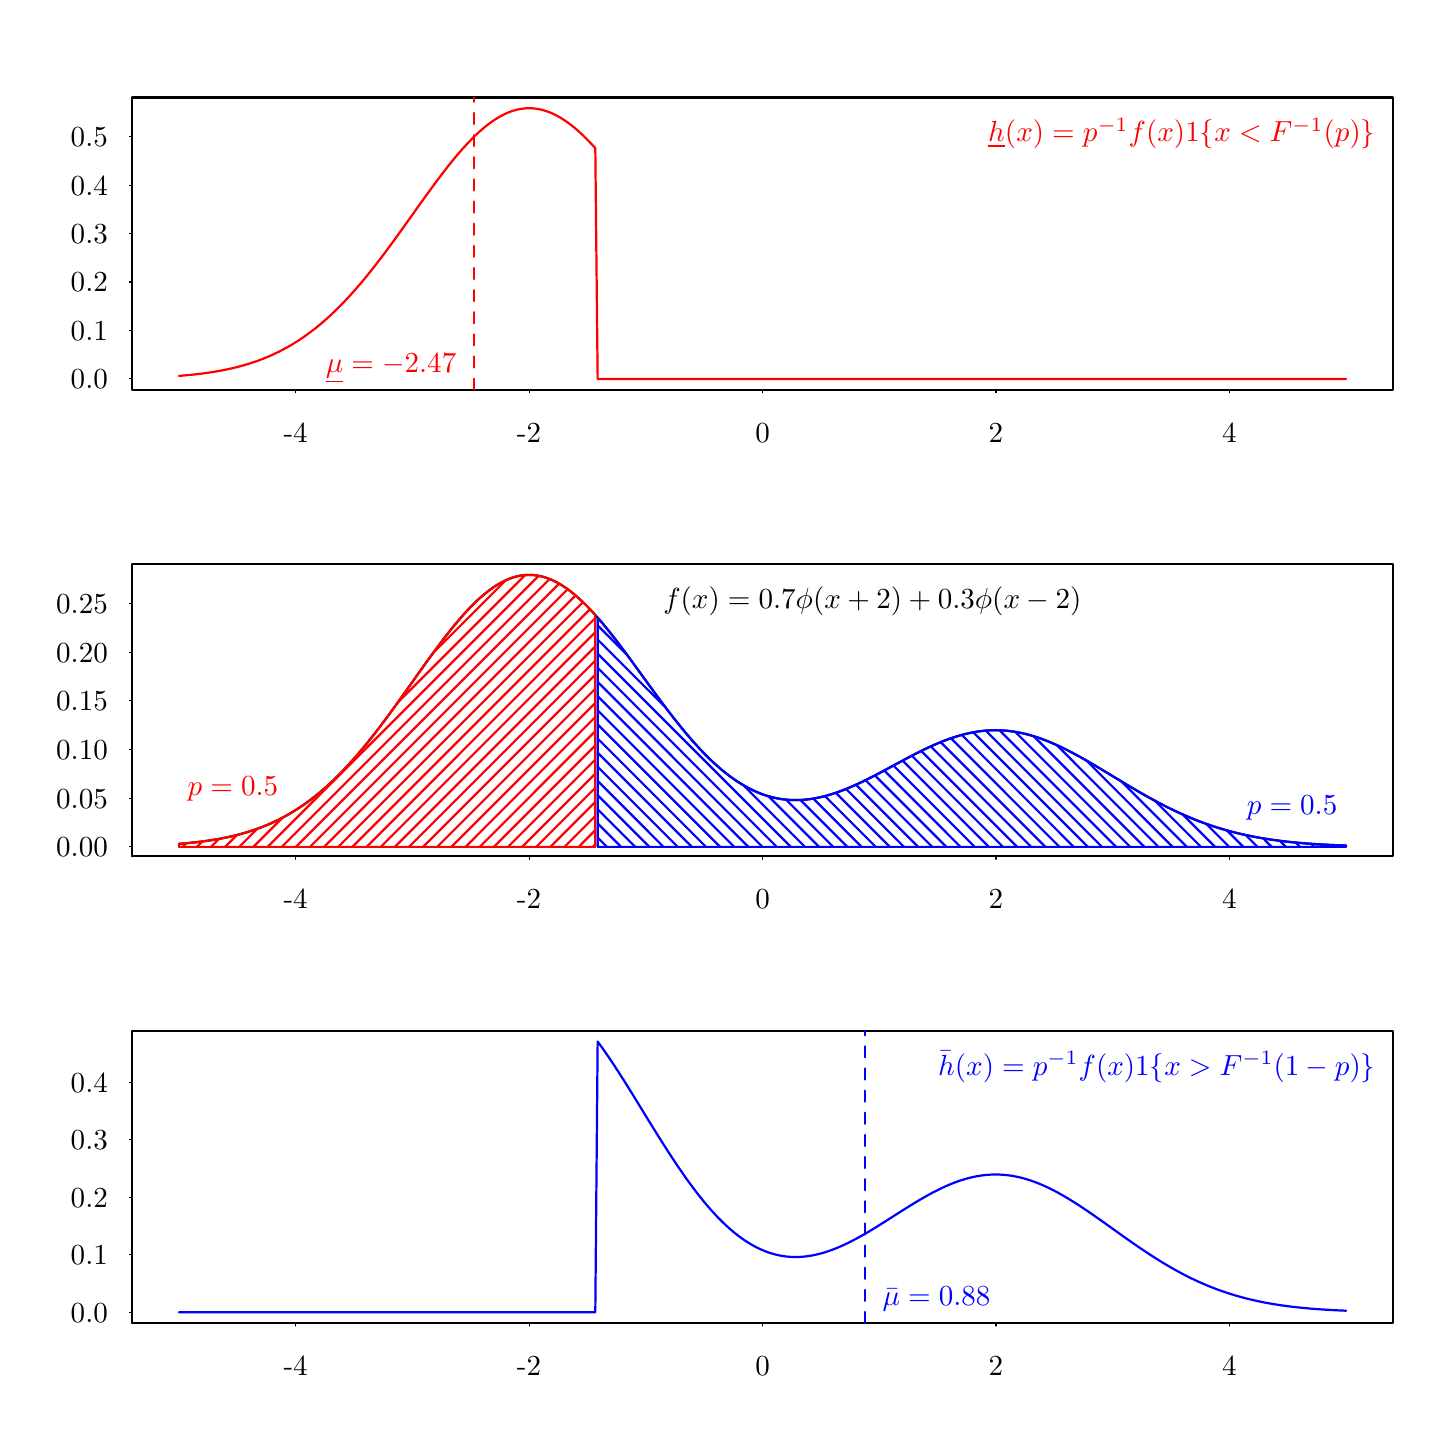
\begin{tikzpicture}[x=1pt,y=1pt]
\definecolor{fillColor}{RGB}{255,255,255}
\path[use as bounding box,fill=fillColor,fill opacity=0.00] (0,0) rectangle (505.89,505.89);
\begin{scope}
\path[clip] ( 37.80,375.06) rectangle (493.29,480.69);
\definecolor{drawColor}{RGB}{255,0,0}

\path[draw=drawColor,line width= 0.8pt,line join=round,line cap=round] ( 54.67,380.06) --
	( 55.52,380.13) --
	( 56.36,380.20) --
	( 57.21,380.27) --
	( 58.05,380.35) --
	( 58.90,380.43) --
	( 59.74,380.52) --
	( 60.59,380.61) --
	( 61.43,380.71) --
	( 62.28,380.81) --
	( 63.12,380.91) --
	( 63.97,381.03) --
	( 64.81,381.14) --
	( 65.66,381.27) --
	( 66.50,381.40) --
	( 67.35,381.53) --
	( 68.19,381.67) --
	( 69.04,381.82) --
	( 69.88,381.98) --
	( 70.73,382.14) --
	( 71.57,382.31) --
	( 72.42,382.49) --
	( 73.26,382.67) --
	( 74.11,382.87) --
	( 74.95,383.07) --
	( 75.80,383.28) --
	( 76.64,383.50) --
	( 77.49,383.73) --
	( 78.34,383.97) --
	( 79.18,384.22) --
	( 80.03,384.48) --
	( 80.87,384.75) --
	( 81.72,385.03) --
	( 82.56,385.32) --
	( 83.41,385.62) --
	( 84.25,385.94) --
	( 85.10,386.27) --
	( 85.94,386.60) --
	( 86.79,386.96) --
	( 87.63,387.32) --
	( 88.48,387.70) --
	( 89.32,388.09) --
	( 90.17,388.50) --
	( 91.01,388.91) --
	( 91.86,389.35) --
	( 92.70,389.79) --
	( 93.55,390.26) --
	( 94.39,390.73) --
	( 95.24,391.23) --
	( 96.08,391.74) --
	( 96.93,392.26) --
	( 97.77,392.80) --
	( 98.62,393.36) --
	( 99.47,393.93) --
	(100.31,394.52) --
	(101.16,395.12) --
	(102.00,395.75) --
	(102.85,396.39) --
	(103.69,397.04) --
	(104.54,397.72) --
	(105.38,398.41) --
	(106.23,399.12) --
	(107.07,399.84) --
	(107.92,400.59) --
	(108.76,401.35) --
	(109.61,402.13) --
	(110.45,402.93) --
	(111.30,403.74) --
	(112.14,404.57) --
	(112.99,405.42) --
	(113.83,406.28) --
	(114.68,407.17) --
	(115.52,408.07) --
	(116.37,408.98) --
	(117.21,409.92) --
	(118.06,410.86) --
	(118.90,411.83) --
	(119.75,412.81) --
	(120.59,413.80) --
	(121.44,414.82) --
	(122.29,415.84) --
	(123.13,416.88) --
	(123.98,417.93) --
	(124.82,419.00) --
	(125.67,420.08) --
	(126.51,421.17) --
	(127.36,422.27) --
	(128.20,423.38) --
	(129.05,424.50) --
	(129.89,425.64) --
	(130.74,426.78) --
	(131.58,427.93) --
	(132.43,429.09) --
	(133.27,430.25) --
	(134.12,431.42) --
	(134.96,432.60) --
	(135.81,433.78) --
	(136.65,434.96) --
	(137.50,436.15) --
	(138.34,437.34) --
	(139.19,438.52) --
	(140.03,439.71) --
	(140.88,440.90) --
	(141.72,442.09) --
	(142.57,443.27) --
	(143.41,444.45) --
	(144.26,445.62) --
	(145.11,446.78) --
	(145.95,447.94) --
	(146.80,449.09) --
	(147.64,450.24) --
	(148.49,451.37) --
	(149.33,452.49) --
	(150.18,453.59) --
	(151.02,454.68) --
	(151.87,455.76) --
	(152.71,456.82) --
	(153.56,457.87) --
	(154.40,458.90) --
	(155.25,459.90) --
	(156.09,460.89) --
	(156.94,461.86) --
	(157.78,462.80) --
	(158.63,463.72) --
	(159.47,464.62) --
	(160.32,465.49) --
	(161.16,466.34) --
	(162.01,467.15) --
	(162.85,467.94) --
	(163.70,468.71) --
	(164.54,469.44) --
	(165.39,470.14) --
	(166.24,470.81) --
	(167.08,471.44) --
	(167.93,472.05) --
	(168.77,472.62) --
	(169.62,473.15) --
	(170.46,473.65) --
	(171.31,474.12) --
	(172.15,474.55) --
	(173.00,474.94) --
	(173.84,475.30) --
	(174.69,475.62) --
	(175.53,475.90) --
	(176.38,476.14) --
	(177.22,476.34) --
	(178.07,476.51) --
	(178.91,476.63) --
	(179.76,476.72) --
	(180.60,476.77) --
	(181.45,476.78) --
	(182.29,476.75) --
	(183.14,476.68) --
	(183.98,476.57) --
	(184.83,476.42) --
	(185.67,476.24) --
	(186.52,476.01) --
	(187.36,475.75) --
	(188.21,475.45) --
	(189.06,475.11) --
	(189.90,474.74) --
	(190.75,474.32) --
	(191.59,473.88) --
	(192.44,473.39) --
	(193.28,472.87) --
	(194.13,472.32) --
	(194.97,471.73) --
	(195.82,471.11) --
	(196.66,470.46) --
	(197.51,469.78) --
	(198.35,469.06) --
	(199.20,468.32) --
	(200.04,467.55) --
	(200.89,466.75) --
	(201.73,465.92) --
	(202.58,465.06) --
	(203.42,464.18) --
	(204.27,463.28) --
	(205.11,462.35) --
	(205.96,378.97) --
	(206.80,378.97) --
	(207.65,378.97) --
	(208.49,378.97) --
	(209.34,378.97) --
	(210.19,378.97) --
	(211.03,378.97) --
	(211.88,378.97) --
	(212.72,378.97) --
	(213.57,378.97) --
	(214.41,378.97) --
	(215.26,378.97) --
	(216.10,378.97) --
	(216.95,378.97) --
	(217.79,378.97) --
	(218.64,378.97) --
	(219.48,378.97) --
	(220.33,378.97) --
	(221.17,378.97) --
	(222.02,378.97) --
	(222.86,378.97) --
	(223.71,378.97) --
	(224.55,378.97) --
	(225.40,378.97) --
	(226.24,378.97) --
	(227.09,378.97) --
	(227.93,378.97) --
	(228.78,378.97) --
	(229.62,378.97) --
	(230.47,378.97) --
	(231.31,378.97) --
	(232.16,378.97) --
	(233.01,378.97) --
	(233.85,378.97) --
	(234.70,378.97) --
	(235.54,378.97) --
	(236.39,378.97) --
	(237.23,378.97) --
	(238.08,378.97) --
	(238.92,378.97) --
	(239.77,378.97) --
	(240.61,378.97) --
	(241.46,378.97) --
	(242.30,378.97) --
	(243.15,378.97) --
	(243.99,378.97) --
	(244.84,378.97) --
	(245.68,378.97) --
	(246.53,378.97) --
	(247.37,378.97) --
	(248.22,378.97) --
	(249.06,378.97) --
	(249.91,378.97) --
	(250.75,378.97) --
	(251.60,378.97) --
	(252.44,378.97) --
	(253.29,378.97) --
	(254.13,378.97) --
	(254.98,378.97) --
	(255.83,378.97) --
	(256.67,378.97) --
	(257.52,378.97) --
	(258.36,378.97) --
	(259.21,378.97) --
	(260.05,378.97) --
	(260.90,378.97) --
	(261.74,378.97) --
	(262.59,378.97) --
	(263.43,378.97) --
	(264.28,378.97) --
	(265.12,378.97) --
	(265.97,378.97) --
	(266.81,378.97) --
	(267.66,378.97) --
	(268.50,378.97) --
	(269.35,378.97) --
	(270.19,378.97) --
	(271.04,378.97) --
	(271.88,378.97) --
	(272.73,378.97) --
	(273.57,378.97) --
	(274.42,378.97) --
	(275.26,378.97) --
	(276.11,378.97) --
	(276.96,378.97) --
	(277.80,378.97) --
	(278.65,378.97) --
	(279.49,378.97) --
	(280.34,378.97) --
	(281.18,378.97) --
	(282.03,378.97) --
	(282.87,378.97) --
	(283.72,378.97) --
	(284.56,378.97) --
	(285.41,378.97) --
	(286.25,378.97) --
	(287.10,378.97) --
	(287.94,378.97) --
	(288.79,378.97) --
	(289.63,378.97) --
	(290.48,378.97) --
	(291.32,378.97) --
	(292.17,378.97) --
	(293.01,378.97) --
	(293.86,378.97) --
	(294.70,378.97) --
	(295.55,378.97) --
	(296.39,378.97) --
	(297.24,378.97) --
	(298.08,378.97) --
	(298.93,378.97) --
	(299.78,378.97) --
	(300.62,378.97) --
	(301.47,378.97) --
	(302.31,378.97) --
	(303.16,378.97) --
	(304.00,378.97) --
	(304.85,378.97) --
	(305.69,378.97) --
	(306.54,378.97) --
	(307.38,378.97) --
	(308.23,378.97) --
	(309.07,378.97) --
	(309.92,378.97) --
	(310.76,378.97) --
	(311.61,378.97) --
	(312.45,378.97) --
	(313.30,378.97) --
	(314.14,378.97) --
	(314.99,378.97) --
	(315.83,378.97) --
	(316.68,378.97) --
	(317.52,378.97) --
	(318.37,378.97) --
	(319.21,378.97) --
	(320.06,378.97) --
	(320.90,378.97) --
	(321.75,378.97) --
	(322.60,378.97) --
	(323.44,378.97) --
	(324.29,378.97) --
	(325.13,378.97) --
	(325.98,378.97) --
	(326.82,378.97) --
	(327.67,378.97) --
	(328.51,378.97) --
	(329.36,378.97) --
	(330.20,378.97) --
	(331.05,378.97) --
	(331.89,378.97) --
	(332.74,378.97) --
	(333.58,378.97) --
	(334.43,378.97) --
	(335.27,378.97) --
	(336.12,378.97) --
	(336.96,378.97) --
	(337.81,378.97) --
	(338.65,378.97) --
	(339.50,378.97) --
	(340.34,378.97) --
	(341.19,378.97) --
	(342.03,378.97) --
	(342.88,378.97) --
	(343.73,378.97) --
	(344.57,378.97) --
	(345.42,378.97) --
	(346.26,378.97) --
	(347.11,378.97) --
	(347.95,378.97) --
	(348.80,378.97) --
	(349.64,378.97) --
	(350.49,378.97) --
	(351.33,378.97) --
	(352.18,378.97) --
	(353.02,378.97) --
	(353.87,378.97) --
	(354.71,378.97) --
	(355.56,378.97) --
	(356.40,378.97) --
	(357.25,378.97) --
	(358.09,378.97) --
	(358.94,378.97) --
	(359.78,378.97) --
	(360.63,378.97) --
	(361.47,378.97) --
	(362.32,378.97) --
	(363.16,378.97) --
	(364.01,378.97) --
	(364.85,378.97) --
	(365.70,378.97) --
	(366.55,378.97) --
	(367.39,378.97) --
	(368.24,378.97) --
	(369.08,378.97) --
	(369.93,378.97) --
	(370.77,378.97) --
	(371.62,378.97) --
	(372.46,378.97) --
	(373.31,378.97) --
	(374.15,378.97) --
	(375.00,378.97) --
	(375.84,378.97) --
	(376.69,378.97) --
	(377.53,378.97) --
	(378.38,378.97) --
	(379.22,378.97) --
	(380.07,378.97) --
	(380.91,378.97) --
	(381.76,378.97) --
	(382.60,378.97) --
	(383.45,378.97) --
	(384.29,378.97) --
	(385.14,378.97) --
	(385.98,378.97) --
	(386.83,378.97) --
	(387.68,378.97) --
	(388.52,378.97) --
	(389.37,378.97) --
	(390.21,378.97) --
	(391.06,378.97) --
	(391.90,378.97) --
	(392.75,378.97) --
	(393.59,378.97) --
	(394.44,378.97) --
	(395.28,378.97) --
	(396.13,378.97) --
	(396.97,378.97) --
	(397.82,378.97) --
	(398.66,378.97) --
	(399.51,378.97) --
	(400.35,378.97) --
	(401.20,378.97) --
	(402.04,378.97) --
	(402.89,378.97) --
	(403.73,378.97) --
	(404.58,378.97) --
	(405.42,378.97) --
	(406.27,378.97) --
	(407.11,378.97) --
	(407.96,378.97) --
	(408.80,378.97) --
	(409.65,378.97) --
	(410.50,378.97) --
	(411.34,378.97) --
	(412.19,378.97) --
	(413.03,378.97) --
	(413.88,378.97) --
	(414.72,378.97) --
	(415.57,378.97) --
	(416.41,378.97) --
	(417.26,378.97) --
	(418.10,378.97) --
	(418.95,378.97) --
	(419.79,378.97) --
	(420.64,378.97) --
	(421.48,378.97) --
	(422.33,378.97) --
	(423.17,378.97) --
	(424.02,378.97) --
	(424.86,378.97) --
	(425.71,378.97) --
	(426.55,378.97) --
	(427.40,378.97) --
	(428.24,378.97) --
	(429.09,378.97) --
	(429.93,378.97) --
	(430.78,378.97) --
	(431.62,378.97) --
	(432.47,378.97) --
	(433.32,378.97) --
	(434.16,378.97) --
	(435.01,378.97) --
	(435.85,378.97) --
	(436.70,378.97) --
	(437.54,378.97) --
	(438.39,378.97) --
	(439.23,378.97) --
	(440.08,378.97) --
	(440.92,378.97) --
	(441.77,378.97) --
	(442.61,378.97) --
	(443.46,378.97) --
	(444.30,378.97) --
	(445.15,378.97) --
	(445.99,378.97) --
	(446.84,378.97) --
	(447.68,378.97) --
	(448.53,378.97) --
	(449.37,378.97) --
	(450.22,378.97) --
	(451.06,378.97) --
	(451.91,378.97) --
	(452.75,378.97) --
	(453.60,378.97) --
	(454.45,378.97) --
	(455.29,378.97) --
	(456.14,378.97) --
	(456.98,378.97) --
	(457.83,378.97) --
	(458.67,378.97) --
	(459.52,378.97) --
	(460.36,378.97) --
	(461.21,378.97) --
	(462.05,378.97) --
	(462.90,378.97) --
	(463.74,378.97) --
	(464.59,378.97) --
	(465.43,378.97) --
	(466.28,378.97) --
	(467.12,378.97) --
	(467.97,378.97) --
	(468.81,378.97) --
	(469.66,378.97) --
	(470.50,378.97) --
	(471.35,378.97) --
	(472.19,378.97) --
	(473.04,378.97) --
	(473.88,378.97) --
	(474.73,378.97) --
	(475.57,378.97) --
	(476.42,378.97);
\end{scope}
\begin{scope}
\path[clip] (  0.00,  0.00) rectangle (505.89,505.89);
\definecolor{drawColor}{RGB}{0,0,0}

\path[draw=drawColor,line width= 0.4pt,line join=round,line cap=round] ( 96.84,375.06) -- (434.25,375.06);

\path[draw=drawColor,line width= 0.4pt,line join=round,line cap=round] ( 96.84,375.06) -- ( 96.84,374.00);

\path[draw=drawColor,line width= 0.4pt,line join=round,line cap=round] (181.19,375.06) -- (181.19,374.00);

\path[draw=drawColor,line width= 0.4pt,line join=round,line cap=round] (265.54,375.06) -- (265.54,374.00);

\path[draw=drawColor,line width= 0.4pt,line join=round,line cap=round] (349.89,375.06) -- (349.89,374.00);

\path[draw=drawColor,line width= 0.4pt,line join=round,line cap=round] (434.25,375.06) -- (434.25,374.00);

\node[text=drawColor,anchor=base,inner sep=0pt, outer sep=0pt, scale=  1.05] at ( 96.84,356.16) {-4};

\node[text=drawColor,anchor=base,inner sep=0pt, outer sep=0pt, scale=  1.05] at (181.19,356.16) {-2};

\node[text=drawColor,anchor=base,inner sep=0pt, outer sep=0pt, scale=  1.05] at (265.54,356.16) {0};

\node[text=drawColor,anchor=base,inner sep=0pt, outer sep=0pt, scale=  1.05] at (349.89,356.16) {2};

\node[text=drawColor,anchor=base,inner sep=0pt, outer sep=0pt, scale=  1.05] at (434.25,356.16) {4};

\path[draw=drawColor,line width= 0.4pt,line join=round,line cap=round] ( 37.80,378.97) -- ( 37.80,466.52);

\path[draw=drawColor,line width= 0.4pt,line join=round,line cap=round] ( 37.80,378.97) -- ( 36.74,378.97);

\path[draw=drawColor,line width= 0.4pt,line join=round,line cap=round] ( 37.80,396.48) -- ( 36.74,396.48);

\path[draw=drawColor,line width= 0.4pt,line join=round,line cap=round] ( 37.80,413.99) -- ( 36.74,413.99);

\path[draw=drawColor,line width= 0.4pt,line join=round,line cap=round] ( 37.80,431.50) -- ( 36.74,431.50);

\path[draw=drawColor,line width= 0.4pt,line join=round,line cap=round] ( 37.80,449.01) -- ( 36.74,449.01);

\path[draw=drawColor,line width= 0.4pt,line join=round,line cap=round] ( 37.80,466.52) -- ( 36.74,466.52);

\node[text=drawColor,anchor=base east,inner sep=0pt, outer sep=0pt, scale=  1.05] at ( 28.98,375.36) {0.0};

\node[text=drawColor,anchor=base east,inner sep=0pt, outer sep=0pt, scale=  1.05] at ( 28.98,392.87) {0.1};

\node[text=drawColor,anchor=base east,inner sep=0pt, outer sep=0pt, scale=  1.05] at ( 28.98,410.38) {0.2};

\node[text=drawColor,anchor=base east,inner sep=0pt, outer sep=0pt, scale=  1.05] at ( 28.98,427.88) {0.3};

\node[text=drawColor,anchor=base east,inner sep=0pt, outer sep=0pt, scale=  1.05] at ( 28.98,445.39) {0.4};

\node[text=drawColor,anchor=base east,inner sep=0pt, outer sep=0pt, scale=  1.05] at ( 28.98,462.90) {0.5};

\path[draw=drawColor,line width= 0.8pt,line join=round,line cap=round] ( 37.80,375.06) --
	(493.29,375.06) --
	(493.29,480.69) --
	( 37.80,480.69) --
	( 37.80,375.06);
\end{scope}
\begin{scope}
\path[clip] ( 37.80,375.06) rectangle (493.29,480.69);
\definecolor{drawColor}{RGB}{255,0,0}

\node[text=drawColor,anchor=base east,inner sep=0pt, outer sep=0pt, scale=  1.05] at (486.99,464.59) {$\underline{h}(x) = p^{-1}f(x) 1\{x < F^{-1}(p)\}$};

\path[draw=drawColor,line width= 0.8pt,dash pattern=on 4pt off 4pt ,line join=round,line cap=round] (161.18,375.06) -- (161.18,480.69);

\node[text=drawColor,anchor=base east,inner sep=0pt, outer sep=0pt, scale=  1.05] at (154.88,381.45) {$\underline{\mu} = -2.47$};
\end{scope}
\begin{scope}
\path[clip] ( 37.80,206.43) rectangle (493.29,312.06);
\definecolor{drawColor}{RGB}{0,0,0}

\path[draw=drawColor,line width= 0.8pt,line join=round,line cap=round] ( 54.67,210.97) --
	( 55.52,211.03) --
	( 56.36,211.10) --
	( 57.21,211.18) --
	( 58.05,211.26) --
	( 58.90,211.34) --
	( 59.74,211.43) --
	( 60.59,211.52) --
	( 61.43,211.62) --
	( 62.28,211.72) --
	( 63.12,211.83) --
	( 63.97,211.94) --
	( 64.81,212.06) --
	( 65.66,212.18) --
	( 66.50,212.31) --
	( 67.35,212.45) --
	( 68.19,212.59) --
	( 69.04,212.74) --
	( 69.88,212.89) --
	( 70.73,213.06) --
	( 71.57,213.23) --
	( 72.42,213.41) --
	( 73.26,213.59) --
	( 74.11,213.79) --
	( 74.95,213.99) --
	( 75.80,214.20) --
	( 76.64,214.42) --
	( 77.49,214.65) --
	( 78.34,214.90) --
	( 79.18,215.15) --
	( 80.03,215.41) --
	( 80.87,215.68) --
	( 81.72,215.96) --
	( 82.56,216.25) --
	( 83.41,216.56) --
	( 84.25,216.87) --
	( 85.10,217.20) --
	( 85.94,217.54) --
	( 86.79,217.90) --
	( 87.63,218.26) --
	( 88.48,218.64) --
	( 89.32,219.04) --
	( 90.17,219.44) --
	( 91.01,219.86) --
	( 91.86,220.30) --
	( 92.70,220.75) --
	( 93.55,221.21) --
	( 94.39,221.69) --
	( 95.24,222.19) --
	( 96.08,222.70) --
	( 96.93,223.23) --
	( 97.77,223.77) --
	( 98.62,224.33) --
	( 99.47,224.90) --
	(100.31,225.49) --
	(101.16,226.10) --
	(102.00,226.73) --
	(102.85,227.37) --
	(103.69,228.03) --
	(104.54,228.71) --
	(105.38,229.40) --
	(106.23,230.12) --
	(107.07,230.85) --
	(107.92,231.59) --
	(108.76,232.36) --
	(109.61,233.14) --
	(110.45,233.94) --
	(111.30,234.76) --
	(112.14,235.59) --
	(112.99,236.45) --
	(113.83,237.32) --
	(114.68,238.20) --
	(115.52,239.11) --
	(116.37,240.03) --
	(117.21,240.97) --
	(118.06,241.92) --
	(118.90,242.89) --
	(119.75,243.87) --
	(120.59,244.87) --
	(121.44,245.89) --
	(122.29,246.92) --
	(123.13,247.96) --
	(123.98,249.02) --
	(124.82,250.09) --
	(125.67,251.17) --
	(126.51,252.27) --
	(127.36,253.38) --
	(128.20,254.50) --
	(129.05,255.62) --
	(129.89,256.76) --
	(130.74,257.91) --
	(131.58,259.07) --
	(132.43,260.23) --
	(133.27,261.40) --
	(134.12,262.58) --
	(134.96,263.76) --
	(135.81,264.94) --
	(136.65,266.13) --
	(137.50,267.32) --
	(138.34,268.52) --
	(139.19,269.71) --
	(140.03,270.91) --
	(140.88,272.10) --
	(141.72,273.29) --
	(142.57,274.48) --
	(143.41,275.66) --
	(144.26,276.84) --
	(145.11,278.01) --
	(145.95,279.18) --
	(146.80,280.33) --
	(147.64,281.48) --
	(148.49,282.61) --
	(149.33,283.74) --
	(150.18,284.85) --
	(151.02,285.95) --
	(151.87,287.03) --
	(152.71,288.10) --
	(153.56,289.15) --
	(154.40,290.18) --
	(155.25,291.19) --
	(156.09,292.19) --
	(156.94,293.16) --
	(157.78,294.11) --
	(158.63,295.03) --
	(159.47,295.93) --
	(160.32,296.81) --
	(161.16,297.66) --
	(162.01,298.48) --
	(162.85,299.27) --
	(163.70,300.04) --
	(164.54,300.77) --
	(165.39,301.47) --
	(166.24,302.15) --
	(167.08,302.79) --
	(167.93,303.39) --
	(168.77,303.97) --
	(169.62,304.51) --
	(170.46,305.01) --
	(171.31,305.48) --
	(172.15,305.91) --
	(173.00,306.30) --
	(173.84,306.66) --
	(174.69,306.98) --
	(175.53,307.26) --
	(176.38,307.50) --
	(177.22,307.71) --
	(178.07,307.88) --
	(178.91,308.00) --
	(179.76,308.09) --
	(180.60,308.14) --
	(181.45,308.15) --
	(182.29,308.12) --
	(183.14,308.05) --
	(183.98,307.94) --
	(184.83,307.79) --
	(185.67,307.60) --
	(186.52,307.38) --
	(187.36,307.11) --
	(188.21,306.81) --
	(189.06,306.47) --
	(189.90,306.10) --
	(190.75,305.68) --
	(191.59,305.23) --
	(192.44,304.75) --
	(193.28,304.22) --
	(194.13,303.67) --
	(194.97,303.08) --
	(195.82,302.46) --
	(196.66,301.80) --
	(197.51,301.12) --
	(198.35,300.40) --
	(199.20,299.65) --
	(200.04,298.87) --
	(200.89,298.07) --
	(201.73,297.24) --
	(202.58,296.38) --
	(203.42,295.49) --
	(204.27,294.59) --
	(205.11,293.65) --
	(205.96,292.70) --
	(206.80,291.73) --
	(207.65,290.73) --
	(208.49,289.72) --
	(209.34,288.68) --
	(210.19,287.63) --
	(211.03,286.57) --
	(211.88,285.49) --
	(212.72,284.40) --
	(213.57,283.29) --
	(214.41,282.18) --
	(215.26,281.05) --
	(216.10,279.91) --
	(216.95,278.77) --
	(217.79,277.62) --
	(218.64,276.46) --
	(219.48,275.30) --
	(220.33,274.14) --
	(221.17,272.97) --
	(222.02,271.81) --
	(222.86,270.64) --
	(223.71,269.47) --
	(224.55,268.31) --
	(225.40,267.15) --
	(226.24,265.99) --
	(227.09,264.84) --
	(227.93,263.69) --
	(228.78,262.55) --
	(229.62,261.42) --
	(230.47,260.29) --
	(231.31,259.18) --
	(232.16,258.08) --
	(233.01,256.98) --
	(233.85,255.90) --
	(234.70,254.83) --
	(235.54,253.78) --
	(236.39,252.74) --
	(237.23,251.71) --
	(238.08,250.70) --
	(238.92,249.71) --
	(239.77,248.73) --
	(240.61,247.77) --
	(241.46,246.82) --
	(242.30,245.90) --
	(243.15,244.99) --
	(243.99,244.10) --
	(244.84,243.24) --
	(245.68,242.39) --
	(246.53,241.56) --
	(247.37,240.76) --
	(248.22,239.97) --
	(249.06,239.21) --
	(249.91,238.47) --
	(250.75,237.75) --
	(251.60,237.05) --
	(252.44,236.38) --
	(253.29,235.73) --
	(254.13,235.10) --
	(254.98,234.49) --
	(255.83,233.91) --
	(256.67,233.35) --
	(257.52,232.81) --
	(258.36,232.30) --
	(259.21,231.81) --
	(260.05,231.34) --
	(260.90,230.90) --
	(261.74,230.48) --
	(262.59,230.08) --
	(263.43,229.70) --
	(264.28,229.35) --
	(265.12,229.03) --
	(265.97,228.72) --
	(266.81,228.44) --
	(267.66,228.18) --
	(268.50,227.94) --
	(269.35,227.73) --
	(270.19,227.54) --
	(271.04,227.37) --
	(271.88,227.22) --
	(272.73,227.09) --
	(273.57,226.99) --
	(274.42,226.90) --
	(275.26,226.84) --
	(276.11,226.80) --
	(276.96,226.78) --
	(277.80,226.77) --
	(278.65,226.79) --
	(279.49,226.83) --
	(280.34,226.88) --
	(281.18,226.96) --
	(282.03,227.05) --
	(282.87,227.16) --
	(283.72,227.29) --
	(284.56,227.44) --
	(285.41,227.60) --
	(286.25,227.78) --
	(287.10,227.97) --
	(287.94,228.18) --
	(288.79,228.41) --
	(289.63,228.65) --
	(290.48,228.91) --
	(291.32,229.18) --
	(292.17,229.46) --
	(293.01,229.76) --
	(293.86,230.07) --
	(294.70,230.39) --
	(295.55,230.72) --
	(296.39,231.07) --
	(297.24,231.42) --
	(298.08,231.79) --
	(298.93,232.16) --
	(299.78,232.55) --
	(300.62,232.94) --
	(301.47,233.34) --
	(302.31,233.75) --
	(303.16,234.16) --
	(304.00,234.59) --
	(304.85,235.01) --
	(305.69,235.45) --
	(306.54,235.89) --
	(307.38,236.33) --
	(308.23,236.78) --
	(309.07,237.23) --
	(309.92,237.68) --
	(310.76,238.13) --
	(311.61,238.59) --
	(312.45,239.05) --
	(313.30,239.50) --
	(314.14,239.96) --
	(314.99,240.41) --
	(315.83,240.87) --
	(316.68,241.32) --
	(317.52,241.77) --
	(318.37,242.22) --
	(319.21,242.66) --
	(320.06,243.10) --
	(320.90,243.53) --
	(321.75,243.96) --
	(322.60,244.38) --
	(323.44,244.80) --
	(324.29,245.21) --
	(325.13,245.61) --
	(325.98,246.00) --
	(326.82,246.39) --
	(327.67,246.76) --
	(328.51,247.13) --
	(329.36,247.48) --
	(330.20,247.83) --
	(331.05,248.16) --
	(331.89,248.49) --
	(332.74,248.80) --
	(333.58,249.09) --
	(334.43,249.38) --
	(335.27,249.65) --
	(336.12,249.91) --
	(336.96,250.16) --
	(337.81,250.39) --
	(338.65,250.61) --
	(339.50,250.81) --
	(340.34,251.00) --
	(341.19,251.17) --
	(342.03,251.33) --
	(342.88,251.47) --
	(343.73,251.60) --
	(344.57,251.71) --
	(345.42,251.80) --
	(346.26,251.88) --
	(347.11,251.94) --
	(347.95,251.98) --
	(348.80,252.01) --
	(349.64,252.02) --
	(350.49,252.01) --
	(351.33,251.99) --
	(352.18,251.95) --
	(353.02,251.89) --
	(353.87,251.82) --
	(354.71,251.73) --
	(355.56,251.63) --
	(356.40,251.51) --
	(357.25,251.37) --
	(358.09,251.21) --
	(358.94,251.04) --
	(359.78,250.86) --
	(360.63,250.66) --
	(361.47,250.44) --
	(362.32,250.21) --
	(363.16,249.96) --
	(364.01,249.70) --
	(364.85,249.43) --
	(365.70,249.14) --
	(366.55,248.84) --
	(367.39,248.52) --
	(368.24,248.19) --
	(369.08,247.85) --
	(369.93,247.50) --
	(370.77,247.13) --
	(371.62,246.76) --
	(372.46,246.37) --
	(373.31,245.98) --
	(374.15,245.57) --
	(375.00,245.15) --
	(375.84,244.73) --
	(376.69,244.29) --
	(377.53,243.85) --
	(378.38,243.40) --
	(379.22,242.94) --
	(380.07,242.48) --
	(380.91,242.01) --
	(381.76,241.53) --
	(382.60,241.05) --
	(383.45,240.56) --
	(384.29,240.07) --
	(385.14,239.58) --
	(385.98,239.08) --
	(386.83,238.57) --
	(387.68,238.07) --
	(388.52,237.56) --
	(389.37,237.05) --
	(390.21,236.54) --
	(391.06,236.03) --
	(391.90,235.52) --
	(392.75,235.01) --
	(393.59,234.50) --
	(394.44,233.98) --
	(395.28,233.48) --
	(396.13,232.97) --
	(396.97,232.46) --
	(397.82,231.96) --
	(398.66,231.46) --
	(399.51,230.96) --
	(400.35,230.46) --
	(401.20,229.97) --
	(402.04,229.48) --
	(402.89,229.00) --
	(403.73,228.52) --
	(404.58,228.04) --
	(405.42,227.57) --
	(406.27,227.11) --
	(407.11,226.65) --
	(407.96,226.20) --
	(408.80,225.75) --
	(409.65,225.31) --
	(410.50,224.87) --
	(411.34,224.45) --
	(412.19,224.02) --
	(413.03,223.61) --
	(413.88,223.20) --
	(414.72,222.80) --
	(415.57,222.40) --
	(416.41,222.02) --
	(417.26,221.64) --
	(418.10,221.26) --
	(418.95,220.90) --
	(419.79,220.54) --
	(420.64,220.19) --
	(421.48,219.85) --
	(422.33,219.51) --
	(423.17,219.18) --
	(424.02,218.86) --
	(424.86,218.55) --
	(425.71,218.24) --
	(426.55,217.95) --
	(427.40,217.66) --
	(428.24,217.37) --
	(429.09,217.10) --
	(429.93,216.83) --
	(430.78,216.57) --
	(431.62,216.32) --
	(432.47,216.07) --
	(433.32,215.83) --
	(434.16,215.60) --
	(435.01,215.37) --
	(435.85,215.15) --
	(436.70,214.94) --
	(437.54,214.73) --
	(438.39,214.53) --
	(439.23,214.34) --
	(440.08,214.16) --
	(440.92,213.98) --
	(441.77,213.80) --
	(442.61,213.63) --
	(443.46,213.47) --
	(444.30,213.31) --
	(445.15,213.16) --
	(445.99,213.02) --
	(446.84,212.87) --
	(447.68,212.74) --
	(448.53,212.61) --
	(449.37,212.48) --
	(450.22,212.36) --
	(451.06,212.25) --
	(451.91,212.13) --
	(452.75,212.03) --
	(453.60,211.92) --
	(454.45,211.82) --
	(455.29,211.73) --
	(456.14,211.64) --
	(456.98,211.55) --
	(457.83,211.47) --
	(458.67,211.39) --
	(459.52,211.31) --
	(460.36,211.24) --
	(461.21,211.17) --
	(462.05,211.10) --
	(462.90,211.04) --
	(463.74,210.98) --
	(464.59,210.92) --
	(465.43,210.86) --
	(466.28,210.81) --
	(467.12,210.76) --
	(467.97,210.71) --
	(468.81,210.67) --
	(469.66,210.62) --
	(470.50,210.58) --
	(471.35,210.54) --
	(472.19,210.50) --
	(473.04,210.47) --
	(473.88,210.43) --
	(474.73,210.40) --
	(475.57,210.37) --
	(476.42,210.34);
\end{scope}
\begin{scope}
\path[clip] (  0.00,  0.00) rectangle (505.89,505.89);
\definecolor{drawColor}{RGB}{0,0,0}

\path[draw=drawColor,line width= 0.4pt,line join=round,line cap=round] ( 96.84,206.43) -- (434.25,206.43);

\path[draw=drawColor,line width= 0.4pt,line join=round,line cap=round] ( 96.84,206.43) -- ( 96.84,205.37);

\path[draw=drawColor,line width= 0.4pt,line join=round,line cap=round] (181.19,206.43) -- (181.19,205.37);

\path[draw=drawColor,line width= 0.4pt,line join=round,line cap=round] (265.54,206.43) -- (265.54,205.37);

\path[draw=drawColor,line width= 0.4pt,line join=round,line cap=round] (349.89,206.43) -- (349.89,205.37);

\path[draw=drawColor,line width= 0.4pt,line join=round,line cap=round] (434.25,206.43) -- (434.25,205.37);

\node[text=drawColor,anchor=base,inner sep=0pt, outer sep=0pt, scale=  1.05] at ( 96.84,187.53) {-4};

\node[text=drawColor,anchor=base,inner sep=0pt, outer sep=0pt, scale=  1.05] at (181.19,187.53) {-2};

\node[text=drawColor,anchor=base,inner sep=0pt, outer sep=0pt, scale=  1.05] at (265.54,187.53) {0};

\node[text=drawColor,anchor=base,inner sep=0pt, outer sep=0pt, scale=  1.05] at (349.89,187.53) {2};

\node[text=drawColor,anchor=base,inner sep=0pt, outer sep=0pt, scale=  1.05] at (434.25,187.53) {4};

\path[draw=drawColor,line width= 0.4pt,line join=round,line cap=round] ( 37.80,209.87) -- ( 37.80,297.84);

\path[draw=drawColor,line width= 0.4pt,line join=round,line cap=round] ( 37.80,209.87) -- ( 36.74,209.87);

\path[draw=drawColor,line width= 0.4pt,line join=round,line cap=round] ( 37.80,227.47) -- ( 36.74,227.47);

\path[draw=drawColor,line width= 0.4pt,line join=round,line cap=round] ( 37.80,245.06) -- ( 36.74,245.06);

\path[draw=drawColor,line width= 0.4pt,line join=round,line cap=round] ( 37.80,262.65) -- ( 36.74,262.65);

\path[draw=drawColor,line width= 0.4pt,line join=round,line cap=round] ( 37.80,280.25) -- ( 36.74,280.25);

\path[draw=drawColor,line width= 0.4pt,line join=round,line cap=round] ( 37.80,297.84) -- ( 36.74,297.84);

\node[text=drawColor,anchor=base east,inner sep=0pt, outer sep=0pt, scale=  1.05] at ( 28.98,206.26) {0.00};

\node[text=drawColor,anchor=base east,inner sep=0pt, outer sep=0pt, scale=  1.05] at ( 28.98,223.85) {0.05};

\node[text=drawColor,anchor=base east,inner sep=0pt, outer sep=0pt, scale=  1.05] at ( 28.98,241.44) {0.10};

\node[text=drawColor,anchor=base east,inner sep=0pt, outer sep=0pt, scale=  1.05] at ( 28.98,259.04) {0.15};

\node[text=drawColor,anchor=base east,inner sep=0pt, outer sep=0pt, scale=  1.05] at ( 28.98,276.63) {0.20};

\node[text=drawColor,anchor=base east,inner sep=0pt, outer sep=0pt, scale=  1.05] at ( 28.98,294.22) {0.25};

\path[draw=drawColor,line width= 0.8pt,line join=round,line cap=round] ( 37.80,206.43) --
	(493.29,206.43) --
	(493.29,312.06) --
	( 37.80,312.06) --
	( 37.80,206.43);
\end{scope}
\begin{scope}
\path[clip] ( 37.80,206.43) rectangle (493.29,312.06);
\definecolor{drawColor}{RGB}{255,0,0}

\path[draw=drawColor,line width= 0.8pt,line join=round,line cap=round] ( 56.02,209.87) -- ( 57.34,211.19);

\path[draw=drawColor,line width= 0.8pt,line join=round,line cap=round] ( 61.13,209.87) -- ( 63.08,211.82);

\path[draw=drawColor,line width= 0.8pt,line join=round,line cap=round] ( 66.24,209.87) -- ( 69.12,212.75);

\path[draw=drawColor,line width= 0.8pt,line join=round,line cap=round] ( 71.36,209.87) -- ( 75.64,214.16);

\path[draw=drawColor,line width= 0.8pt,line join=round,line cap=round] ( 76.47,209.87) -- ( 83.00,216.41);

\path[draw=drawColor,line width= 0.8pt,line join=round,line cap=round] (146.45,279.86) -- (172.80,306.21);

\path[draw=drawColor,line width= 0.8pt,line join=round,line cap=round] ( 81.58,209.87) -- ( 92.16,220.46);

\path[draw=drawColor,line width= 0.8pt,line join=round,line cap=round] (133.71,262.01) -- (179.79,308.09);

\path[draw=drawColor,line width= 0.8pt,line join=round,line cap=round] ( 86.69,209.87) -- (184.64,307.82);

\path[draw=drawColor,line width= 0.8pt,line join=round,line cap=round] ( 91.80,209.87) -- (188.58,306.66);

\path[draw=drawColor,line width= 0.8pt,line join=round,line cap=round] ( 96.91,209.87) -- (192.02,304.99);

\path[draw=drawColor,line width= 0.8pt,line join=round,line cap=round] (102.02,209.87) -- (195.12,302.97);

\path[draw=drawColor,line width= 0.8pt,line join=round,line cap=round] (107.13,209.87) -- (197.97,300.72);

\path[draw=drawColor,line width= 0.8pt,line join=round,line cap=round] (112.24,209.87) -- (200.65,298.29);

\path[draw=drawColor,line width= 0.8pt,line join=round,line cap=round] (117.35,209.87) -- (203.20,295.73);

\path[draw=drawColor,line width= 0.8pt,line join=round,line cap=round] (122.46,209.87) -- (205.11,292.53);

\path[draw=drawColor,line width= 0.8pt,line join=round,line cap=round] (127.57,209.87) -- (205.11,287.42);

\path[draw=drawColor,line width= 0.8pt,line join=round,line cap=round] (132.68,209.87) -- (205.11,282.31);

\path[draw=drawColor,line width= 0.8pt,line join=round,line cap=round] (137.79,209.87) -- (205.11,277.20);

\path[draw=drawColor,line width= 0.8pt,line join=round,line cap=round] (142.90,209.87) -- (205.11,272.09);

\path[draw=drawColor,line width= 0.8pt,line join=round,line cap=round] (148.01,209.87) -- (205.11,266.98);

\path[draw=drawColor,line width= 0.8pt,line join=round,line cap=round] (153.12,209.87) -- (205.11,261.87);

\path[draw=drawColor,line width= 0.8pt,line join=round,line cap=round] (158.23,209.87) -- (205.11,256.76);

\path[draw=drawColor,line width= 0.8pt,line join=round,line cap=round] (163.34,209.87) -- (205.11,251.65);

\path[draw=drawColor,line width= 0.8pt,line join=round,line cap=round] (168.45,209.87) -- (205.11,246.54);

\path[draw=drawColor,line width= 0.8pt,line join=round,line cap=round] (173.56,209.87) -- (205.11,241.43);

\path[draw=drawColor,line width= 0.8pt,line join=round,line cap=round] (178.67,209.87) -- (205.11,236.32);

\path[draw=drawColor,line width= 0.8pt,line join=round,line cap=round] (183.78,209.87) -- (205.11,231.21);

\path[draw=drawColor,line width= 0.8pt,line join=round,line cap=round] (188.89,209.87) -- (205.11,226.10);

\path[draw=drawColor,line width= 0.8pt,line join=round,line cap=round] (194.00,209.87) -- (205.11,220.99);

\path[draw=drawColor,line width= 0.8pt,line join=round,line cap=round] (199.11,209.87) -- (205.11,215.88);

\path[draw=drawColor,line width= 0.8pt,line join=round,line cap=round] (204.22,209.87) -- (205.11,210.77);

\path[draw=drawColor,line width= 0.8pt,line join=round,line cap=round] ( 54.67,209.87) --
	( 55.52,209.87) --
	( 56.36,209.87) --
	( 57.21,209.87) --
	( 58.05,209.87) --
	( 58.90,209.87) --
	( 59.74,209.87) --
	( 60.59,209.87) --
	( 61.43,209.87) --
	( 62.28,209.87) --
	( 63.12,209.87) --
	( 63.97,209.87) --
	( 64.81,209.87) --
	( 65.66,209.87) --
	( 66.50,209.87) --
	( 67.35,209.87) --
	( 68.19,209.87) --
	( 69.04,209.87) --
	( 69.88,209.87) --
	( 70.73,209.87) --
	( 71.57,209.87) --
	( 72.42,209.87) --
	( 73.26,209.87) --
	( 74.11,209.87) --
	( 74.95,209.87) --
	( 75.80,209.87) --
	( 76.64,209.87) --
	( 77.49,209.87) --
	( 78.34,209.87) --
	( 79.18,209.87) --
	( 80.03,209.87) --
	( 80.87,209.87) --
	( 81.72,209.87) --
	( 82.56,209.87) --
	( 83.41,209.87) --
	( 84.25,209.87) --
	( 85.10,209.87) --
	( 85.94,209.87) --
	( 86.79,209.87) --
	( 87.63,209.87) --
	( 88.48,209.87) --
	( 89.32,209.87) --
	( 90.17,209.87) --
	( 91.01,209.87) --
	( 91.86,209.87) --
	( 92.70,209.87) --
	( 93.55,209.87) --
	( 94.39,209.87) --
	( 95.24,209.87) --
	( 96.08,209.87) --
	( 96.93,209.87) --
	( 97.77,209.87) --
	( 98.62,209.87) --
	( 99.47,209.87) --
	(100.31,209.87) --
	(101.16,209.87) --
	(102.00,209.87) --
	(102.85,209.87) --
	(103.69,209.87) --
	(104.54,209.87) --
	(105.38,209.87) --
	(106.23,209.87) --
	(107.07,209.87) --
	(107.92,209.87) --
	(108.76,209.87) --
	(109.61,209.87) --
	(110.45,209.87) --
	(111.30,209.87) --
	(112.14,209.87) --
	(112.99,209.87) --
	(113.83,209.87) --
	(114.68,209.87) --
	(115.52,209.87) --
	(116.37,209.87) --
	(117.21,209.87) --
	(118.06,209.87) --
	(118.90,209.87) --
	(119.75,209.87) --
	(120.59,209.87) --
	(121.44,209.87) --
	(122.29,209.87) --
	(123.13,209.87) --
	(123.98,209.87) --
	(124.82,209.87) --
	(125.67,209.87) --
	(126.51,209.87) --
	(127.36,209.87) --
	(128.20,209.87) --
	(129.05,209.87) --
	(129.89,209.87) --
	(130.74,209.87) --
	(131.58,209.87) --
	(132.43,209.87) --
	(133.27,209.87) --
	(134.12,209.87) --
	(134.96,209.87) --
	(135.81,209.87) --
	(136.65,209.87) --
	(137.50,209.87) --
	(138.34,209.87) --
	(139.19,209.87) --
	(140.03,209.87) --
	(140.88,209.87) --
	(141.72,209.87) --
	(142.57,209.87) --
	(143.41,209.87) --
	(144.26,209.87) --
	(145.11,209.87) --
	(145.95,209.87) --
	(146.80,209.87) --
	(147.64,209.87) --
	(148.49,209.87) --
	(149.33,209.87) --
	(150.18,209.87) --
	(151.02,209.87) --
	(151.87,209.87) --
	(152.71,209.87) --
	(153.56,209.87) --
	(154.40,209.87) --
	(155.25,209.87) --
	(156.09,209.87) --
	(156.94,209.87) --
	(157.78,209.87) --
	(158.63,209.87) --
	(159.47,209.87) --
	(160.32,209.87) --
	(161.16,209.87) --
	(162.01,209.87) --
	(162.85,209.87) --
	(163.70,209.87) --
	(164.54,209.87) --
	(165.39,209.87) --
	(166.24,209.87) --
	(167.08,209.87) --
	(167.93,209.87) --
	(168.77,209.87) --
	(169.62,209.87) --
	(170.46,209.87) --
	(171.31,209.87) --
	(172.15,209.87) --
	(173.00,209.87) --
	(173.84,209.87) --
	(174.69,209.87) --
	(175.53,209.87) --
	(176.38,209.87) --
	(177.22,209.87) --
	(178.07,209.87) --
	(178.91,209.87) --
	(179.76,209.87) --
	(180.60,209.87) --
	(181.45,209.87) --
	(182.29,209.87) --
	(183.14,209.87) --
	(183.98,209.87) --
	(184.83,209.87) --
	(185.67,209.87) --
	(186.52,209.87) --
	(187.36,209.87) --
	(188.21,209.87) --
	(189.06,209.87) --
	(189.90,209.87) --
	(190.75,209.87) --
	(191.59,209.87) --
	(192.44,209.87) --
	(193.28,209.87) --
	(194.13,209.87) --
	(194.97,209.87) --
	(195.82,209.87) --
	(196.66,209.87) --
	(197.51,209.87) --
	(198.35,209.87) --
	(199.20,209.87) --
	(200.04,209.87) --
	(200.89,209.87) --
	(201.73,209.87) --
	(202.58,209.87) --
	(203.42,209.87) --
	(204.27,209.87) --
	(205.11,209.87) --
	(205.11,293.65) --
	(204.27,294.59) --
	(203.42,295.49) --
	(202.58,296.38) --
	(201.73,297.24) --
	(200.89,298.07) --
	(200.04,298.87) --
	(199.20,299.65) --
	(198.35,300.40) --
	(197.51,301.12) --
	(196.66,301.80) --
	(195.82,302.46) --
	(194.97,303.08) --
	(194.13,303.67) --
	(193.28,304.22) --
	(192.44,304.75) --
	(191.59,305.23) --
	(190.75,305.68) --
	(189.90,306.10) --
	(189.06,306.47) --
	(188.21,306.81) --
	(187.36,307.11) --
	(186.52,307.38) --
	(185.67,307.60) --
	(184.83,307.79) --
	(183.98,307.94) --
	(183.14,308.05) --
	(182.29,308.12) --
	(181.45,308.15) --
	(180.60,308.14) --
	(179.76,308.09) --
	(178.91,308.00) --
	(178.07,307.88) --
	(177.22,307.71) --
	(176.38,307.50) --
	(175.53,307.26) --
	(174.69,306.98) --
	(173.84,306.66) --
	(173.00,306.30) --
	(172.15,305.91) --
	(171.31,305.48) --
	(170.46,305.01) --
	(169.62,304.51) --
	(168.77,303.97) --
	(167.93,303.39) --
	(167.08,302.79) --
	(166.24,302.15) --
	(165.39,301.47) --
	(164.54,300.77) --
	(163.70,300.04) --
	(162.85,299.27) --
	(162.01,298.48) --
	(161.16,297.66) --
	(160.32,296.81) --
	(159.47,295.93) --
	(158.63,295.03) --
	(157.78,294.11) --
	(156.94,293.16) --
	(156.09,292.19) --
	(155.25,291.19) --
	(154.40,290.18) --
	(153.56,289.15) --
	(152.71,288.10) --
	(151.87,287.03) --
	(151.02,285.95) --
	(150.18,284.85) --
	(149.33,283.74) --
	(148.49,282.61) --
	(147.64,281.48) --
	(146.80,280.33) --
	(145.95,279.18) --
	(145.11,278.01) --
	(144.26,276.84) --
	(143.41,275.66) --
	(142.57,274.48) --
	(141.72,273.29) --
	(140.88,272.10) --
	(140.03,270.91) --
	(139.19,269.71) --
	(138.34,268.52) --
	(137.50,267.32) --
	(136.65,266.13) --
	(135.81,264.94) --
	(134.96,263.76) --
	(134.12,262.58) --
	(133.27,261.40) --
	(132.43,260.23) --
	(131.58,259.07) --
	(130.74,257.91) --
	(129.89,256.76) --
	(129.05,255.62) --
	(128.20,254.50) --
	(127.36,253.38) --
	(126.51,252.27) --
	(125.67,251.17) --
	(124.82,250.09) --
	(123.98,249.02) --
	(123.13,247.96) --
	(122.29,246.92) --
	(121.44,245.89) --
	(120.59,244.87) --
	(119.75,243.87) --
	(118.90,242.89) --
	(118.06,241.92) --
	(117.21,240.97) --
	(116.37,240.03) --
	(115.52,239.11) --
	(114.68,238.20) --
	(113.83,237.32) --
	(112.99,236.45) --
	(112.14,235.59) --
	(111.30,234.76) --
	(110.45,233.94) --
	(109.61,233.14) --
	(108.76,232.36) --
	(107.92,231.59) --
	(107.07,230.85) --
	(106.23,230.12) --
	(105.38,229.40) --
	(104.54,228.71) --
	(103.69,228.03) --
	(102.85,227.37) --
	(102.00,226.73) --
	(101.16,226.10) --
	(100.31,225.49) --
	( 99.47,224.90) --
	( 98.62,224.33) --
	( 97.77,223.77) --
	( 96.93,223.23) --
	( 96.08,222.70) --
	( 95.24,222.19) --
	( 94.39,221.69) --
	( 93.55,221.21) --
	( 92.70,220.75) --
	( 91.86,220.30) --
	( 91.01,219.86) --
	( 90.17,219.44) --
	( 89.32,219.04) --
	( 88.48,218.64) --
	( 87.63,218.26) --
	( 86.79,217.90) --
	( 85.94,217.54) --
	( 85.10,217.20) --
	( 84.25,216.87) --
	( 83.41,216.56) --
	( 82.56,216.25) --
	( 81.72,215.96) --
	( 80.87,215.68) --
	( 80.03,215.41) --
	( 79.18,215.15) --
	( 78.34,214.90) --
	( 77.49,214.65) --
	( 76.64,214.42) --
	( 75.80,214.20) --
	( 74.95,213.99) --
	( 74.11,213.79) --
	( 73.26,213.59) --
	( 72.42,213.41) --
	( 71.57,213.23) --
	( 70.73,213.06) --
	( 69.88,212.89) --
	( 69.04,212.74) --
	( 68.19,212.59) --
	( 67.35,212.45) --
	( 66.50,212.31) --
	( 65.66,212.18) --
	( 64.81,212.06) --
	( 63.97,211.94) --
	( 63.12,211.83) --
	( 62.28,211.72) --
	( 61.43,211.62) --
	( 60.59,211.52) --
	( 59.74,211.43) --
	( 58.90,211.34) --
	( 58.05,211.26) --
	( 57.21,211.18) --
	( 56.36,211.10) --
	( 55.52,211.03) --
	( 54.67,210.97) --
	( 54.67,209.87);

\node[text=drawColor,anchor=base east,inner sep=0pt, outer sep=0pt, scale=  1.05] at ( 90.54,228.58) {$p = 0.5$};
\definecolor{drawColor}{RGB}{0,0,255}

\path[draw=drawColor,line width= 0.8pt,line join=round,line cap=round] (209.33,209.87) -- (205.96,213.25);

\path[draw=drawColor,line width= 0.8pt,line join=round,line cap=round] (214.44,209.87) -- (205.96,218.36);

\path[draw=drawColor,line width= 0.8pt,line join=round,line cap=round] (219.55,209.87) -- (205.96,223.47);

\path[draw=drawColor,line width= 0.8pt,line join=round,line cap=round] (224.66,209.87) -- (205.96,228.58);

\path[draw=drawColor,line width= 0.8pt,line join=round,line cap=round] (229.77,209.87) -- (205.96,233.69);

\path[draw=drawColor,line width= 0.8pt,line join=round,line cap=round] (234.88,209.87) -- (205.96,238.80);

\path[draw=drawColor,line width= 0.8pt,line join=round,line cap=round] (239.99,209.87) -- (205.96,243.91);

\path[draw=drawColor,line width= 0.8pt,line join=round,line cap=round] (245.10,209.87) -- (205.96,249.02);

\path[draw=drawColor,line width= 0.8pt,line join=round,line cap=round] (250.21,209.87) -- (205.96,254.13);

\path[draw=drawColor,line width= 0.8pt,line join=round,line cap=round] (255.32,209.87) -- (205.96,259.24);

\path[draw=drawColor,line width= 0.8pt,line join=round,line cap=round] (260.43,209.87) -- (205.96,264.35);

\path[draw=drawColor,line width= 0.8pt,line join=round,line cap=round] (265.54,209.87) -- (205.96,269.46);

\path[draw=drawColor,line width= 0.8pt,line join=round,line cap=round] (270.66,209.87) -- (205.96,274.57);

\path[draw=drawColor,line width= 0.8pt,line join=round,line cap=round] (275.77,209.87) -- (205.96,279.68);

\path[draw=drawColor,line width= 0.8pt,line join=round,line cap=round] (280.88,209.87) -- (258.58,232.17);

\path[draw=drawColor,line width= 0.8pt,line join=round,line cap=round] (230.51,260.24) -- (205.96,284.79);

\path[draw=drawColor,line width= 0.8pt,line join=round,line cap=round] (285.99,209.87) -- (267.69,228.17);

\path[draw=drawColor,line width= 0.8pt,line join=round,line cap=round] (216.54,279.32) -- (205.96,289.90);

\path[draw=drawColor,line width= 0.8pt,line join=round,line cap=round] (291.10,209.87) -- (274.03,226.94);

\path[draw=drawColor,line width= 0.8pt,line join=round,line cap=round] (296.21,209.87) -- (279.26,226.82);

\path[draw=drawColor,line width= 0.8pt,line join=round,line cap=round] (301.32,209.87) -- (283.87,227.32);

\path[draw=drawColor,line width= 0.8pt,line join=round,line cap=round] (306.43,209.87) -- (288.08,228.22);

\path[draw=drawColor,line width= 0.8pt,line join=round,line cap=round] (311.54,209.87) -- (292.01,229.41);

\path[draw=drawColor,line width= 0.8pt,line join=round,line cap=round] (316.65,209.87) -- (295.73,230.79);

\path[draw=drawColor,line width= 0.8pt,line join=round,line cap=round] (321.76,209.87) -- (299.30,232.33);

\path[draw=drawColor,line width= 0.8pt,line join=round,line cap=round] (326.87,209.87) -- (302.77,233.97);

\path[draw=drawColor,line width= 0.8pt,line join=round,line cap=round] (331.98,209.87) -- (306.16,235.69);

\path[draw=drawColor,line width= 0.8pt,line join=round,line cap=round] (337.09,209.87) -- (309.51,237.46);

\path[draw=drawColor,line width= 0.8pt,line join=round,line cap=round] (342.20,209.87) -- (312.83,239.25);

\path[draw=drawColor,line width= 0.8pt,line join=round,line cap=round] (347.31,209.87) -- (316.15,241.04);

\path[draw=drawColor,line width= 0.8pt,line join=round,line cap=round] (352.42,209.87) -- (319.49,242.80);

\path[draw=drawColor,line width= 0.8pt,line join=round,line cap=round] (357.53,209.87) -- (322.88,244.52);

\path[draw=drawColor,line width= 0.8pt,line join=round,line cap=round] (362.64,209.87) -- (326.35,246.17);

\path[draw=drawColor,line width= 0.8pt,line join=round,line cap=round] (367.75,209.87) -- (329.91,247.71);

\path[draw=drawColor,line width= 0.8pt,line join=round,line cap=round] (372.86,209.87) -- (333.63,249.11);

\path[draw=drawColor,line width= 0.8pt,line join=round,line cap=round] (377.97,209.87) -- (337.53,250.32);

\path[draw=drawColor,line width= 0.8pt,line join=round,line cap=round] (383.08,209.87) -- (341.69,251.27);

\path[draw=drawColor,line width= 0.8pt,line join=round,line cap=round] (388.19,209.87) -- (346.20,251.87);

\path[draw=drawColor,line width= 0.8pt,line join=round,line cap=round] (393.30,209.87) -- (351.18,251.99);

\path[draw=drawColor,line width= 0.8pt,line join=round,line cap=round] (398.41,209.87) -- (356.85,251.43);

\path[draw=drawColor,line width= 0.8pt,line join=round,line cap=round] (403.52,209.87) -- (363.56,249.84);

\path[draw=drawColor,line width= 0.8pt,line join=round,line cap=round] (408.63,209.87) -- (371.86,246.65);

\path[draw=drawColor,line width= 0.8pt,line join=round,line cap=round] (413.74,209.87) -- (382.52,241.10);

\path[draw=drawColor,line width= 0.8pt,line join=round,line cap=round] (418.85,209.87) -- (395.21,233.52);

\path[draw=drawColor,line width= 0.8pt,line join=round,line cap=round] (423.96,209.87) -- (407.27,226.57);

\path[draw=drawColor,line width= 0.8pt,line join=round,line cap=round] (429.07,209.87) -- (417.36,221.59);

\path[draw=drawColor,line width= 0.8pt,line join=round,line cap=round] (434.18,209.87) -- (425.87,218.19);

\path[draw=drawColor,line width= 0.8pt,line join=round,line cap=round] (439.29,209.87) -- (433.35,215.82);

\path[draw=drawColor,line width= 0.8pt,line join=round,line cap=round] (444.40,209.87) -- (440.14,214.14);

\path[draw=drawColor,line width= 0.8pt,line join=round,line cap=round] (449.51,209.87) -- (446.45,212.94);

\path[draw=drawColor,line width= 0.8pt,line join=round,line cap=round] (454.62,209.87) -- (452.43,212.07);

\path[draw=drawColor,line width= 0.8pt,line join=round,line cap=round] (459.73,209.87) -- (458.17,211.43);

\path[draw=drawColor,line width= 0.8pt,line join=round,line cap=round] (464.85,209.87) -- (463.74,210.98);

\path[draw=drawColor,line width= 0.8pt,line join=round,line cap=round] (469.96,209.87) -- (469.18,210.65);

\path[draw=drawColor,line width= 0.8pt,line join=round,line cap=round] (475.07,209.87) -- (474.53,210.41);

\path[draw=drawColor,line width= 0.8pt,line join=round,line cap=round] (205.96,209.87) --
	(206.80,209.87) --
	(207.65,209.87) --
	(208.49,209.87) --
	(209.34,209.87) --
	(210.19,209.87) --
	(211.03,209.87) --
	(211.88,209.87) --
	(212.72,209.87) --
	(213.57,209.87) --
	(214.41,209.87) --
	(215.26,209.87) --
	(216.10,209.87) --
	(216.95,209.87) --
	(217.79,209.87) --
	(218.64,209.87) --
	(219.48,209.87) --
	(220.33,209.87) --
	(221.17,209.87) --
	(222.02,209.87) --
	(222.86,209.87) --
	(223.71,209.87) --
	(224.55,209.87) --
	(225.40,209.87) --
	(226.24,209.87) --
	(227.09,209.87) --
	(227.93,209.87) --
	(228.78,209.87) --
	(229.62,209.87) --
	(230.47,209.87) --
	(231.31,209.87) --
	(232.16,209.87) --
	(233.01,209.87) --
	(233.85,209.87) --
	(234.70,209.87) --
	(235.54,209.87) --
	(236.39,209.87) --
	(237.23,209.87) --
	(238.08,209.87) --
	(238.92,209.87) --
	(239.77,209.87) --
	(240.61,209.87) --
	(241.46,209.87) --
	(242.30,209.87) --
	(243.15,209.87) --
	(243.99,209.87) --
	(244.84,209.87) --
	(245.68,209.87) --
	(246.53,209.87) --
	(247.37,209.87) --
	(248.22,209.87) --
	(249.06,209.87) --
	(249.91,209.87) --
	(250.75,209.87) --
	(251.60,209.87) --
	(252.44,209.87) --
	(253.29,209.87) --
	(254.13,209.87) --
	(254.98,209.87) --
	(255.83,209.87) --
	(256.67,209.87) --
	(257.52,209.87) --
	(258.36,209.87) --
	(259.21,209.87) --
	(260.05,209.87) --
	(260.90,209.87) --
	(261.74,209.87) --
	(262.59,209.87) --
	(263.43,209.87) --
	(264.28,209.87) --
	(265.12,209.87) --
	(265.97,209.87) --
	(266.81,209.87) --
	(267.66,209.87) --
	(268.50,209.87) --
	(269.35,209.87) --
	(270.19,209.87) --
	(271.04,209.87) --
	(271.88,209.87) --
	(272.73,209.87) --
	(273.57,209.87) --
	(274.42,209.87) --
	(275.26,209.87) --
	(276.11,209.87) --
	(276.96,209.87) --
	(277.80,209.87) --
	(278.65,209.87) --
	(279.49,209.87) --
	(280.34,209.87) --
	(281.18,209.87) --
	(282.03,209.87) --
	(282.87,209.87) --
	(283.72,209.87) --
	(284.56,209.87) --
	(285.41,209.87) --
	(286.25,209.87) --
	(287.10,209.87) --
	(287.94,209.87) --
	(288.79,209.87) --
	(289.63,209.87) --
	(290.48,209.87) --
	(291.32,209.87) --
	(292.17,209.87) --
	(293.01,209.87) --
	(293.86,209.87) --
	(294.70,209.87) --
	(295.55,209.87) --
	(296.39,209.87) --
	(297.24,209.87) --
	(298.08,209.87) --
	(298.93,209.87) --
	(299.78,209.87) --
	(300.62,209.87) --
	(301.47,209.87) --
	(302.31,209.87) --
	(303.16,209.87) --
	(304.00,209.87) --
	(304.85,209.87) --
	(305.69,209.87) --
	(306.54,209.87) --
	(307.38,209.87) --
	(308.23,209.87) --
	(309.07,209.87) --
	(309.92,209.87) --
	(310.76,209.87) --
	(311.61,209.87) --
	(312.45,209.87) --
	(313.30,209.87) --
	(314.14,209.87) --
	(314.99,209.87) --
	(315.83,209.87) --
	(316.68,209.87) --
	(317.52,209.87) --
	(318.37,209.87) --
	(319.21,209.87) --
	(320.06,209.87) --
	(320.90,209.87) --
	(321.75,209.87) --
	(322.60,209.87) --
	(323.44,209.87) --
	(324.29,209.87) --
	(325.13,209.87) --
	(325.98,209.87) --
	(326.82,209.87) --
	(327.67,209.87) --
	(328.51,209.87) --
	(329.36,209.87) --
	(330.20,209.87) --
	(331.05,209.87) --
	(331.89,209.87) --
	(332.74,209.87) --
	(333.58,209.87) --
	(334.43,209.87) --
	(335.27,209.87) --
	(336.12,209.87) --
	(336.96,209.87) --
	(337.81,209.87) --
	(338.65,209.87) --
	(339.50,209.87) --
	(340.34,209.87) --
	(341.19,209.87) --
	(342.03,209.87) --
	(342.88,209.87) --
	(343.73,209.87) --
	(344.57,209.87) --
	(345.42,209.87) --
	(346.26,209.87) --
	(347.11,209.87) --
	(347.95,209.87) --
	(348.80,209.87) --
	(349.64,209.87) --
	(350.49,209.87) --
	(351.33,209.87) --
	(352.18,209.87) --
	(353.02,209.87) --
	(353.87,209.87) --
	(354.71,209.87) --
	(355.56,209.87) --
	(356.40,209.87) --
	(357.25,209.87) --
	(358.09,209.87) --
	(358.94,209.87) --
	(359.78,209.87) --
	(360.63,209.87) --
	(361.47,209.87) --
	(362.32,209.87) --
	(363.16,209.87) --
	(364.01,209.87) --
	(364.85,209.87) --
	(365.70,209.87) --
	(366.55,209.87) --
	(367.39,209.87) --
	(368.24,209.87) --
	(369.08,209.87) --
	(369.93,209.87) --
	(370.77,209.87) --
	(371.62,209.87) --
	(372.46,209.87) --
	(373.31,209.87) --
	(374.15,209.87) --
	(375.00,209.87) --
	(375.84,209.87) --
	(376.69,209.87) --
	(377.53,209.87) --
	(378.38,209.87) --
	(379.22,209.87) --
	(380.07,209.87) --
	(380.91,209.87) --
	(381.76,209.87) --
	(382.60,209.87) --
	(383.45,209.87) --
	(384.29,209.87) --
	(385.14,209.87) --
	(385.98,209.87) --
	(386.83,209.87) --
	(387.68,209.87) --
	(388.52,209.87) --
	(389.37,209.87) --
	(390.21,209.87) --
	(391.06,209.87) --
	(391.90,209.87) --
	(392.75,209.87) --
	(393.59,209.87) --
	(394.44,209.87) --
	(395.28,209.87) --
	(396.13,209.87) --
	(396.97,209.87) --
	(397.82,209.87) --
	(398.66,209.87) --
	(399.51,209.87) --
	(400.35,209.87) --
	(401.20,209.87) --
	(402.04,209.87) --
	(402.89,209.87) --
	(403.73,209.87) --
	(404.58,209.87) --
	(405.42,209.87) --
	(406.27,209.87) --
	(407.11,209.87) --
	(407.96,209.87) --
	(408.80,209.87) --
	(409.65,209.87) --
	(410.50,209.87) --
	(411.34,209.87) --
	(412.19,209.87) --
	(413.03,209.87) --
	(413.88,209.87) --
	(414.72,209.87) --
	(415.57,209.87) --
	(416.41,209.87) --
	(417.26,209.87) --
	(418.10,209.87) --
	(418.95,209.87) --
	(419.79,209.87) --
	(420.64,209.87) --
	(421.48,209.87) --
	(422.33,209.87) --
	(423.17,209.87) --
	(424.02,209.87) --
	(424.86,209.87) --
	(425.71,209.87) --
	(426.55,209.87) --
	(427.40,209.87) --
	(428.24,209.87) --
	(429.09,209.87) --
	(429.93,209.87) --
	(430.78,209.87) --
	(431.62,209.87) --
	(432.47,209.87) --
	(433.32,209.87) --
	(434.16,209.87) --
	(435.01,209.87) --
	(435.85,209.87) --
	(436.70,209.87) --
	(437.54,209.87) --
	(438.39,209.87) --
	(439.23,209.87) --
	(440.08,209.87) --
	(440.92,209.87) --
	(441.77,209.87) --
	(442.61,209.87) --
	(443.46,209.87) --
	(444.30,209.87) --
	(445.15,209.87) --
	(445.99,209.87) --
	(446.84,209.87) --
	(447.68,209.87) --
	(448.53,209.87) --
	(449.37,209.87) --
	(450.22,209.87) --
	(451.06,209.87) --
	(451.91,209.87) --
	(452.75,209.87) --
	(453.60,209.87) --
	(454.45,209.87) --
	(455.29,209.87) --
	(456.14,209.87) --
	(456.98,209.87) --
	(457.83,209.87) --
	(458.67,209.87) --
	(459.52,209.87) --
	(460.36,209.87) --
	(461.21,209.87) --
	(462.05,209.87) --
	(462.90,209.87) --
	(463.74,209.87) --
	(464.59,209.87) --
	(465.43,209.87) --
	(466.28,209.87) --
	(467.12,209.87) --
	(467.97,209.87) --
	(468.81,209.87) --
	(469.66,209.87) --
	(470.50,209.87) --
	(471.35,209.87) --
	(472.19,209.87) --
	(473.04,209.87) --
	(473.88,209.87) --
	(474.73,209.87) --
	(475.57,209.87) --
	(476.42,209.87) --
	(476.42,210.34) --
	(475.57,210.37) --
	(474.73,210.40) --
	(473.88,210.43) --
	(473.04,210.47) --
	(472.19,210.50) --
	(471.35,210.54) --
	(470.50,210.58) --
	(469.66,210.62) --
	(468.81,210.67) --
	(467.97,210.71) --
	(467.12,210.76) --
	(466.28,210.81) --
	(465.43,210.86) --
	(464.59,210.92) --
	(463.74,210.98) --
	(462.90,211.04) --
	(462.05,211.10) --
	(461.21,211.17) --
	(460.36,211.24) --
	(459.52,211.31) --
	(458.67,211.39) --
	(457.83,211.47) --
	(456.98,211.55) --
	(456.14,211.64) --
	(455.29,211.73) --
	(454.45,211.82) --
	(453.60,211.92) --
	(452.75,212.03) --
	(451.91,212.13) --
	(451.06,212.25) --
	(450.22,212.36) --
	(449.37,212.48) --
	(448.53,212.61) --
	(447.68,212.74) --
	(446.84,212.87) --
	(445.99,213.02) --
	(445.15,213.16) --
	(444.30,213.31) --
	(443.46,213.47) --
	(442.61,213.63) --
	(441.77,213.80) --
	(440.92,213.98) --
	(440.08,214.16) --
	(439.23,214.34) --
	(438.39,214.53) --
	(437.54,214.73) --
	(436.70,214.94) --
	(435.85,215.15) --
	(435.01,215.37) --
	(434.16,215.60) --
	(433.32,215.83) --
	(432.47,216.07) --
	(431.62,216.32) --
	(430.78,216.57) --
	(429.93,216.83) --
	(429.09,217.10) --
	(428.24,217.37) --
	(427.40,217.66) --
	(426.55,217.95) --
	(425.71,218.24) --
	(424.86,218.55) --
	(424.02,218.86) --
	(423.17,219.18) --
	(422.33,219.51) --
	(421.48,219.85) --
	(420.64,220.19) --
	(419.79,220.54) --
	(418.95,220.90) --
	(418.10,221.26) --
	(417.26,221.64) --
	(416.41,222.02) --
	(415.57,222.40) --
	(414.72,222.80) --
	(413.88,223.20) --
	(413.03,223.61) --
	(412.19,224.02) --
	(411.34,224.45) --
	(410.50,224.87) --
	(409.65,225.31) --
	(408.80,225.75) --
	(407.96,226.20) --
	(407.11,226.65) --
	(406.27,227.11) --
	(405.42,227.57) --
	(404.58,228.04) --
	(403.73,228.52) --
	(402.89,229.00) --
	(402.04,229.48) --
	(401.20,229.97) --
	(400.35,230.46) --
	(399.51,230.96) --
	(398.66,231.46) --
	(397.82,231.96) --
	(396.97,232.46) --
	(396.13,232.97) --
	(395.28,233.48) --
	(394.44,233.98) --
	(393.59,234.50) --
	(392.75,235.01) --
	(391.90,235.52) --
	(391.06,236.03) --
	(390.21,236.54) --
	(389.37,237.05) --
	(388.52,237.56) --
	(387.68,238.07) --
	(386.83,238.57) --
	(385.98,239.08) --
	(385.14,239.58) --
	(384.29,240.07) --
	(383.45,240.56) --
	(382.60,241.05) --
	(381.76,241.53) --
	(380.91,242.01) --
	(380.07,242.48) --
	(379.22,242.94) --
	(378.38,243.40) --
	(377.53,243.85) --
	(376.69,244.29) --
	(375.84,244.73) --
	(375.00,245.15) --
	(374.15,245.57) --
	(373.31,245.98) --
	(372.46,246.37) --
	(371.62,246.76) --
	(370.77,247.13) --
	(369.93,247.50) --
	(369.08,247.85) --
	(368.24,248.19) --
	(367.39,248.52) --
	(366.55,248.84) --
	(365.70,249.14) --
	(364.85,249.43) --
	(364.01,249.70) --
	(363.16,249.96) --
	(362.32,250.21) --
	(361.47,250.44) --
	(360.63,250.66) --
	(359.78,250.86) --
	(358.94,251.04) --
	(358.09,251.21) --
	(357.25,251.37) --
	(356.40,251.51) --
	(355.56,251.63) --
	(354.71,251.73) --
	(353.87,251.82) --
	(353.02,251.89) --
	(352.18,251.95) --
	(351.33,251.99) --
	(350.49,252.01) --
	(349.64,252.02) --
	(348.80,252.01) --
	(347.95,251.98) --
	(347.11,251.94) --
	(346.26,251.88) --
	(345.42,251.80) --
	(344.57,251.71) --
	(343.73,251.60) --
	(342.88,251.47) --
	(342.03,251.33) --
	(341.19,251.17) --
	(340.34,251.00) --
	(339.50,250.81) --
	(338.65,250.61) --
	(337.81,250.39) --
	(336.96,250.16) --
	(336.12,249.91) --
	(335.27,249.65) --
	(334.43,249.38) --
	(333.58,249.09) --
	(332.74,248.80) --
	(331.89,248.49) --
	(331.05,248.16) --
	(330.20,247.83) --
	(329.36,247.48) --
	(328.51,247.13) --
	(327.67,246.76) --
	(326.82,246.39) --
	(325.98,246.00) --
	(325.13,245.61) --
	(324.29,245.21) --
	(323.44,244.80) --
	(322.60,244.38) --
	(321.75,243.96) --
	(320.90,243.53) --
	(320.06,243.10) --
	(319.21,242.66) --
	(318.37,242.22) --
	(317.52,241.77) --
	(316.68,241.32) --
	(315.83,240.87) --
	(314.99,240.41) --
	(314.14,239.96) --
	(313.30,239.50) --
	(312.45,239.05) --
	(311.61,238.59) --
	(310.76,238.13) --
	(309.92,237.68) --
	(309.07,237.23) --
	(308.23,236.78) --
	(307.38,236.33) --
	(306.54,235.89) --
	(305.69,235.45) --
	(304.85,235.01) --
	(304.00,234.59) --
	(303.16,234.16) --
	(302.31,233.75) --
	(301.47,233.34) --
	(300.62,232.94) --
	(299.78,232.55) --
	(298.93,232.16) --
	(298.08,231.79) --
	(297.24,231.42) --
	(296.39,231.07) --
	(295.55,230.72) --
	(294.70,230.39) --
	(293.86,230.07) --
	(293.01,229.76) --
	(292.17,229.46) --
	(291.32,229.18) --
	(290.48,228.91) --
	(289.63,228.65) --
	(288.79,228.41) --
	(287.94,228.18) --
	(287.10,227.97) --
	(286.25,227.78) --
	(285.41,227.60) --
	(284.56,227.44) --
	(283.72,227.29) --
	(282.87,227.16) --
	(282.03,227.05) --
	(281.18,226.96) --
	(280.34,226.88) --
	(279.49,226.83) --
	(278.65,226.79) --
	(277.80,226.77) --
	(276.96,226.78) --
	(276.11,226.80) --
	(275.26,226.84) --
	(274.42,226.90) --
	(273.57,226.99) --
	(272.73,227.09) --
	(271.88,227.22) --
	(271.04,227.37) --
	(270.19,227.54) --
	(269.35,227.73) --
	(268.50,227.94) --
	(267.66,228.18) --
	(266.81,228.44) --
	(265.97,228.72) --
	(265.12,229.03) --
	(264.28,229.35) --
	(263.43,229.70) --
	(262.59,230.08) --
	(261.74,230.48) --
	(260.90,230.90) --
	(260.05,231.34) --
	(259.21,231.81) --
	(258.36,232.30) --
	(257.52,232.81) --
	(256.67,233.35) --
	(255.83,233.91) --
	(254.98,234.49) --
	(254.13,235.10) --
	(253.29,235.73) --
	(252.44,236.38) --
	(251.60,237.05) --
	(250.75,237.75) --
	(249.91,238.47) --
	(249.06,239.21) --
	(248.22,239.97) --
	(247.37,240.76) --
	(246.53,241.56) --
	(245.68,242.39) --
	(244.84,243.24) --
	(243.99,244.10) --
	(243.15,244.99) --
	(242.30,245.90) --
	(241.46,246.82) --
	(240.61,247.77) --
	(239.77,248.73) --
	(238.92,249.71) --
	(238.08,250.70) --
	(237.23,251.71) --
	(236.39,252.74) --
	(235.54,253.78) --
	(234.70,254.83) --
	(233.85,255.90) --
	(233.01,256.98) --
	(232.16,258.08) --
	(231.31,259.18) --
	(230.47,260.29) --
	(229.62,261.42) --
	(228.78,262.55) --
	(227.93,263.69) --
	(227.09,264.84) --
	(226.24,265.99) --
	(225.40,267.15) --
	(224.55,268.31) --
	(223.71,269.47) --
	(222.86,270.64) --
	(222.02,271.81) --
	(221.17,272.97) --
	(220.33,274.14) --
	(219.48,275.30) --
	(218.64,276.46) --
	(217.79,277.62) --
	(216.95,278.77) --
	(216.10,279.91) --
	(215.26,281.05) --
	(214.41,282.18) --
	(213.57,283.29) --
	(212.72,284.40) --
	(211.88,285.49) --
	(211.03,286.57) --
	(210.19,287.63) --
	(209.34,288.68) --
	(208.49,289.72) --
	(207.65,290.73) --
	(206.80,291.73) --
	(205.96,292.70) --
	(205.96,209.87);

\node[text=drawColor,anchor=base west,inner sep=0pt, outer sep=0pt, scale=  1.05] at (440.55,221.54) {$p = 0.5$};
\definecolor{drawColor}{RGB}{0,0,0}

\node[text=drawColor,anchor=base west,inner sep=0pt, outer sep=0pt, scale=  1.05] at (229.67,295.91) {$f(x) = 0.7 \phi(x + 2)+0.3\phi(x - 2)$};
\end{scope}
\begin{scope}
\path[clip] ( 37.80, 37.80) rectangle (493.29,143.43);
\definecolor{drawColor}{RGB}{0,0,255}

\path[draw=drawColor,line width= 0.8pt,line join=round,line cap=round] ( 54.67, 41.71) --
	( 55.52, 41.71) --
	( 56.36, 41.71) --
	( 57.21, 41.71) --
	( 58.05, 41.71) --
	( 58.90, 41.71) --
	( 59.74, 41.71) --
	( 60.59, 41.71) --
	( 61.43, 41.71) --
	( 62.28, 41.71) --
	( 63.12, 41.71) --
	( 63.97, 41.71) --
	( 64.81, 41.71) --
	( 65.66, 41.71) --
	( 66.50, 41.71) --
	( 67.35, 41.71) --
	( 68.19, 41.71) --
	( 69.04, 41.71) --
	( 69.88, 41.71) --
	( 70.73, 41.71) --
	( 71.57, 41.71) --
	( 72.42, 41.71) --
	( 73.26, 41.71) --
	( 74.11, 41.71) --
	( 74.95, 41.71) --
	( 75.80, 41.71) --
	( 76.64, 41.71) --
	( 77.49, 41.71) --
	( 78.34, 41.71) --
	( 79.18, 41.71) --
	( 80.03, 41.71) --
	( 80.87, 41.71) --
	( 81.72, 41.71) --
	( 82.56, 41.71) --
	( 83.41, 41.71) --
	( 84.25, 41.71) --
	( 85.10, 41.71) --
	( 85.94, 41.71) --
	( 86.79, 41.71) --
	( 87.63, 41.71) --
	( 88.48, 41.71) --
	( 89.32, 41.71) --
	( 90.17, 41.71) --
	( 91.01, 41.71) --
	( 91.86, 41.71) --
	( 92.70, 41.71) --
	( 93.55, 41.71) --
	( 94.39, 41.71) --
	( 95.24, 41.71) --
	( 96.08, 41.71) --
	( 96.93, 41.71) --
	( 97.77, 41.71) --
	( 98.62, 41.71) --
	( 99.47, 41.71) --
	(100.31, 41.71) --
	(101.16, 41.71) --
	(102.00, 41.71) --
	(102.85, 41.71) --
	(103.69, 41.71) --
	(104.54, 41.71) --
	(105.38, 41.71) --
	(106.23, 41.71) --
	(107.07, 41.71) --
	(107.92, 41.71) --
	(108.76, 41.71) --
	(109.61, 41.71) --
	(110.45, 41.71) --
	(111.30, 41.71) --
	(112.14, 41.71) --
	(112.99, 41.71) --
	(113.83, 41.71) --
	(114.68, 41.71) --
	(115.52, 41.71) --
	(116.37, 41.71) --
	(117.21, 41.71) --
	(118.06, 41.71) --
	(118.90, 41.71) --
	(119.75, 41.71) --
	(120.59, 41.71) --
	(121.44, 41.71) --
	(122.29, 41.71) --
	(123.13, 41.71) --
	(123.98, 41.71) --
	(124.82, 41.71) --
	(125.67, 41.71) --
	(126.51, 41.71) --
	(127.36, 41.71) --
	(128.20, 41.71) --
	(129.05, 41.71) --
	(129.89, 41.71) --
	(130.74, 41.71) --
	(131.58, 41.71) --
	(132.43, 41.71) --
	(133.27, 41.71) --
	(134.12, 41.71) --
	(134.96, 41.71) --
	(135.81, 41.71) --
	(136.65, 41.71) --
	(137.50, 41.71) --
	(138.34, 41.71) --
	(139.19, 41.71) --
	(140.03, 41.71) --
	(140.88, 41.71) --
	(141.72, 41.71) --
	(142.57, 41.71) --
	(143.41, 41.71) --
	(144.26, 41.71) --
	(145.11, 41.71) --
	(145.95, 41.71) --
	(146.80, 41.71) --
	(147.64, 41.71) --
	(148.49, 41.71) --
	(149.33, 41.71) --
	(150.18, 41.71) --
	(151.02, 41.71) --
	(151.87, 41.71) --
	(152.71, 41.71) --
	(153.56, 41.71) --
	(154.40, 41.71) --
	(155.25, 41.71) --
	(156.09, 41.71) --
	(156.94, 41.71) --
	(157.78, 41.71) --
	(158.63, 41.71) --
	(159.47, 41.71) --
	(160.32, 41.71) --
	(161.16, 41.71) --
	(162.01, 41.71) --
	(162.85, 41.71) --
	(163.70, 41.71) --
	(164.54, 41.71) --
	(165.39, 41.71) --
	(166.24, 41.71) --
	(167.08, 41.71) --
	(167.93, 41.71) --
	(168.77, 41.71) --
	(169.62, 41.71) --
	(170.46, 41.71) --
	(171.31, 41.71) --
	(172.15, 41.71) --
	(173.00, 41.71) --
	(173.84, 41.71) --
	(174.69, 41.71) --
	(175.53, 41.71) --
	(176.38, 41.71) --
	(177.22, 41.71) --
	(178.07, 41.71) --
	(178.91, 41.71) --
	(179.76, 41.71) --
	(180.60, 41.71) --
	(181.45, 41.71) --
	(182.29, 41.71) --
	(183.14, 41.71) --
	(183.98, 41.71) --
	(184.83, 41.71) --
	(185.67, 41.71) --
	(186.52, 41.71) --
	(187.36, 41.71) --
	(188.21, 41.71) --
	(189.06, 41.71) --
	(189.90, 41.71) --
	(190.75, 41.71) --
	(191.59, 41.71) --
	(192.44, 41.71) --
	(193.28, 41.71) --
	(194.13, 41.71) --
	(194.97, 41.71) --
	(195.82, 41.71) --
	(196.66, 41.71) --
	(197.51, 41.71) --
	(198.35, 41.71) --
	(199.20, 41.71) --
	(200.04, 41.71) --
	(200.89, 41.71) --
	(201.73, 41.71) --
	(202.58, 41.71) --
	(203.42, 41.71) --
	(204.27, 41.71) --
	(205.11, 41.71) --
	(205.96,139.52) --
	(206.80,138.37) --
	(207.65,137.19) --
	(208.49,135.99) --
	(209.34,134.77) --
	(210.19,133.54) --
	(211.03,132.28) --
	(211.88,131.00) --
	(212.72,129.71) --
	(213.57,128.41) --
	(214.41,127.09) --
	(215.26,125.76) --
	(216.10,124.42) --
	(216.95,123.07) --
	(217.79,121.71) --
	(218.64,120.35) --
	(219.48,118.98) --
	(220.33,117.60) --
	(221.17,116.22) --
	(222.02,114.85) --
	(222.86,113.47) --
	(223.71,112.09) --
	(224.55,110.72) --
	(225.40,109.34) --
	(226.24,107.98) --
	(227.09,106.62) --
	(227.93,105.26) --
	(228.78,103.92) --
	(229.62,102.58) --
	(230.47,101.25) --
	(231.31, 99.94) --
	(232.16, 98.63) --
	(233.01, 97.34) --
	(233.85, 96.06) --
	(234.70, 94.80) --
	(235.54, 93.56) --
	(236.39, 92.33) --
	(237.23, 91.11) --
	(238.08, 89.92) --
	(238.92, 88.75) --
	(239.77, 87.59) --
	(240.61, 86.46) --
	(241.46, 85.34) --
	(242.30, 84.25) --
	(243.15, 83.18) --
	(243.99, 82.13) --
	(244.84, 81.11) --
	(245.68, 80.11) --
	(246.53, 79.13) --
	(247.37, 78.18) --
	(248.22, 77.25) --
	(249.06, 76.35) --
	(249.91, 75.48) --
	(250.75, 74.63) --
	(251.60, 73.81) --
	(252.44, 73.01) --
	(253.29, 72.24) --
	(254.13, 71.50) --
	(254.98, 70.78) --
	(255.83, 70.09) --
	(256.67, 69.43) --
	(257.52, 68.80) --
	(258.36, 68.19) --
	(259.21, 67.61) --
	(260.05, 67.06) --
	(260.90, 66.54) --
	(261.74, 66.04) --
	(262.59, 65.57) --
	(263.43, 65.13) --
	(264.28, 64.72) --
	(265.12, 64.33) --
	(265.97, 63.97) --
	(266.81, 63.64) --
	(267.66, 63.33) --
	(268.50, 63.05) --
	(269.35, 62.80) --
	(270.19, 62.57) --
	(271.04, 62.37) --
	(271.88, 62.20) --
	(272.73, 62.05) --
	(273.57, 61.92) --
	(274.42, 61.82) --
	(275.26, 61.75) --
	(276.11, 61.70) --
	(276.96, 61.67) --
	(277.80, 61.67) --
	(278.65, 61.69) --
	(279.49, 61.73) --
	(280.34, 61.80) --
	(281.18, 61.88) --
	(282.03, 61.99) --
	(282.87, 62.13) --
	(283.72, 62.28) --
	(284.56, 62.45) --
	(285.41, 62.64) --
	(286.25, 62.85) --
	(287.10, 63.08) --
	(287.94, 63.33) --
	(288.79, 63.60) --
	(289.63, 63.89) --
	(290.48, 64.19) --
	(291.32, 64.51) --
	(292.17, 64.84) --
	(293.01, 65.19) --
	(293.86, 65.56) --
	(294.70, 65.94) --
	(295.55, 66.33) --
	(296.39, 66.74) --
	(297.24, 67.16) --
	(298.08, 67.59) --
	(298.93, 68.03) --
	(299.78, 68.48) --
	(300.62, 68.95) --
	(301.47, 69.42) --
	(302.31, 69.90) --
	(303.16, 70.40) --
	(304.00, 70.89) --
	(304.85, 71.40) --
	(305.69, 71.91) --
	(306.54, 72.43) --
	(307.38, 72.95) --
	(308.23, 73.48) --
	(309.07, 74.01) --
	(309.92, 74.54) --
	(310.76, 75.08) --
	(311.61, 75.62) --
	(312.45, 76.16) --
	(313.30, 76.70) --
	(314.14, 77.24) --
	(314.99, 77.78) --
	(315.83, 78.31) --
	(316.68, 78.85) --
	(317.52, 79.38) --
	(318.37, 79.90) --
	(319.21, 80.43) --
	(320.06, 80.95) --
	(320.90, 81.46) --
	(321.75, 81.96) --
	(322.60, 82.46) --
	(323.44, 82.95) --
	(324.29, 83.44) --
	(325.13, 83.91) --
	(325.98, 84.37) --
	(326.82, 84.83) --
	(327.67, 85.27) --
	(328.51, 85.70) --
	(329.36, 86.12) --
	(330.20, 86.53) --
	(331.05, 86.92) --
	(331.89, 87.31) --
	(332.74, 87.67) --
	(333.58, 88.03) --
	(334.43, 88.36) --
	(335.27, 88.69) --
	(336.12, 88.99) --
	(336.96, 89.28) --
	(337.81, 89.56) --
	(338.65, 89.81) --
	(339.50, 90.05) --
	(340.34, 90.28) --
	(341.19, 90.48) --
	(342.03, 90.66) --
	(342.88, 90.83) --
	(343.73, 90.98) --
	(344.57, 91.11) --
	(345.42, 91.22) --
	(346.26, 91.31) --
	(347.11, 91.38) --
	(347.95, 91.43) --
	(348.80, 91.47) --
	(349.64, 91.48) --
	(350.49, 91.47) --
	(351.33, 91.45) --
	(352.18, 91.40) --
	(353.02, 91.33) --
	(353.87, 91.25) --
	(354.71, 91.14) --
	(355.56, 91.02) --
	(356.40, 90.87) --
	(357.25, 90.71) --
	(358.09, 90.53) --
	(358.94, 90.33) --
	(359.78, 90.11) --
	(360.63, 89.87) --
	(361.47, 89.61) --
	(362.32, 89.34) --
	(363.16, 89.05) --
	(364.01, 88.74) --
	(364.85, 88.42) --
	(365.70, 88.08) --
	(366.55, 87.72) --
	(367.39, 87.35) --
	(368.24, 86.96) --
	(369.08, 86.56) --
	(369.93, 86.14) --
	(370.77, 85.71) --
	(371.62, 85.27) --
	(372.46, 84.81) --
	(373.31, 84.34) --
	(374.15, 83.86) --
	(375.00, 83.37) --
	(375.84, 82.87) --
	(376.69, 82.36) --
	(377.53, 81.83) --
	(378.38, 81.30) --
	(379.22, 80.76) --
	(380.07, 80.21) --
	(380.91, 79.66) --
	(381.76, 79.09) --
	(382.60, 78.53) --
	(383.45, 77.95) --
	(384.29, 77.37) --
	(385.14, 76.78) --
	(385.98, 76.20) --
	(386.83, 75.60) --
	(387.68, 75.01) --
	(388.52, 74.41) --
	(389.37, 73.81) --
	(390.21, 73.20) --
	(391.06, 72.60) --
	(391.90, 72.00) --
	(392.75, 71.39) --
	(393.59, 70.79) --
	(394.44, 70.18) --
	(395.28, 69.58) --
	(396.13, 68.98) --
	(396.97, 68.38) --
	(397.82, 67.79) --
	(398.66, 67.20) --
	(399.51, 66.61) --
	(400.35, 66.02) --
	(401.20, 65.44) --
	(402.04, 64.87) --
	(402.89, 64.29) --
	(403.73, 63.73) --
	(404.58, 63.17) --
	(405.42, 62.61) --
	(406.27, 62.07) --
	(407.11, 61.52) --
	(407.96, 60.99) --
	(408.80, 60.46) --
	(409.65, 59.94) --
	(410.50, 59.42) --
	(411.34, 58.92) --
	(412.19, 58.42) --
	(413.03, 57.93) --
	(413.88, 57.45) --
	(414.72, 56.97) --
	(415.57, 56.51) --
	(416.41, 56.05) --
	(417.26, 55.60) --
	(418.10, 55.16) --
	(418.95, 54.73) --
	(419.79, 54.31) --
	(420.64, 53.89) --
	(421.48, 53.49) --
	(422.33, 53.09) --
	(423.17, 52.70) --
	(424.02, 52.33) --
	(424.86, 51.96) --
	(425.71, 51.60) --
	(426.55, 51.24) --
	(427.40, 50.90) --
	(428.24, 50.57) --
	(429.09, 50.24) --
	(429.93, 49.93) --
	(430.78, 49.62) --
	(431.62, 49.32) --
	(432.47, 49.03) --
	(433.32, 48.74) --
	(434.16, 48.47) --
	(435.01, 48.20) --
	(435.85, 47.94) --
	(436.70, 47.69) --
	(437.54, 47.45) --
	(438.39, 47.22) --
	(439.23, 46.99) --
	(440.08, 46.77) --
	(440.92, 46.55) --
	(441.77, 46.35) --
	(442.61, 46.15) --
	(443.46, 45.96) --
	(444.30, 45.77) --
	(445.15, 45.59) --
	(445.99, 45.42) --
	(446.84, 45.25) --
	(447.68, 45.09) --
	(448.53, 44.94) --
	(449.37, 44.79) --
	(450.22, 44.65) --
	(451.06, 44.51) --
	(451.91, 44.38) --
	(452.75, 44.25) --
	(453.60, 44.13) --
	(454.45, 44.01) --
	(455.29, 43.90) --
	(456.14, 43.80) --
	(456.98, 43.69) --
	(457.83, 43.59) --
	(458.67, 43.50) --
	(459.52, 43.41) --
	(460.36, 43.32) --
	(461.21, 43.24) --
	(462.05, 43.16) --
	(462.90, 43.09) --
	(463.74, 43.01) --
	(464.59, 42.94) --
	(465.43, 42.88) --
	(466.28, 42.82) --
	(467.12, 42.76) --
	(467.97, 42.70) --
	(468.81, 42.65) --
	(469.66, 42.59) --
	(470.50, 42.55) --
	(471.35, 42.50) --
	(472.19, 42.45) --
	(473.04, 42.41) --
	(473.88, 42.37) --
	(474.73, 42.33) --
	(475.57, 42.30) --
	(476.42, 42.26);
\end{scope}
\begin{scope}
\path[clip] (  0.00,  0.00) rectangle (505.89,505.89);
\definecolor{drawColor}{RGB}{0,0,0}

\path[draw=drawColor,line width= 0.4pt,line join=round,line cap=round] ( 96.84, 37.80) -- (434.25, 37.80);

\path[draw=drawColor,line width= 0.4pt,line join=round,line cap=round] ( 96.84, 37.80) -- ( 96.84, 36.74);

\path[draw=drawColor,line width= 0.4pt,line join=round,line cap=round] (181.19, 37.80) -- (181.19, 36.74);

\path[draw=drawColor,line width= 0.4pt,line join=round,line cap=round] (265.54, 37.80) -- (265.54, 36.74);

\path[draw=drawColor,line width= 0.4pt,line join=round,line cap=round] (349.89, 37.80) -- (349.89, 36.74);

\path[draw=drawColor,line width= 0.4pt,line join=round,line cap=round] (434.25, 37.80) -- (434.25, 36.74);

\node[text=drawColor,anchor=base,inner sep=0pt, outer sep=0pt, scale=  1.05] at ( 96.84, 18.90) {-4};

\node[text=drawColor,anchor=base,inner sep=0pt, outer sep=0pt, scale=  1.05] at (181.19, 18.90) {-2};

\node[text=drawColor,anchor=base,inner sep=0pt, outer sep=0pt, scale=  1.05] at (265.54, 18.90) {0};

\node[text=drawColor,anchor=base,inner sep=0pt, outer sep=0pt, scale=  1.05] at (349.89, 18.90) {2};

\node[text=drawColor,anchor=base,inner sep=0pt, outer sep=0pt, scale=  1.05] at (434.25, 18.90) {4};

\path[draw=drawColor,line width= 0.4pt,line join=round,line cap=round] ( 37.80, 41.71) -- ( 37.80,124.81);

\path[draw=drawColor,line width= 0.4pt,line join=round,line cap=round] ( 37.80, 41.71) -- ( 36.74, 41.71);

\path[draw=drawColor,line width= 0.4pt,line join=round,line cap=round] ( 37.80, 62.49) -- ( 36.74, 62.49);

\path[draw=drawColor,line width= 0.4pt,line join=round,line cap=round] ( 37.80, 83.26) -- ( 36.74, 83.26);

\path[draw=drawColor,line width= 0.4pt,line join=round,line cap=round] ( 37.80,104.04) -- ( 36.74,104.04);

\path[draw=drawColor,line width= 0.4pt,line join=round,line cap=round] ( 37.80,124.81) -- ( 36.74,124.81);

\node[text=drawColor,anchor=base east,inner sep=0pt, outer sep=0pt, scale=  1.05] at ( 28.98, 38.10) {0.0};

\node[text=drawColor,anchor=base east,inner sep=0pt, outer sep=0pt, scale=  1.05] at ( 28.98, 58.87) {0.1};

\node[text=drawColor,anchor=base east,inner sep=0pt, outer sep=0pt, scale=  1.05] at ( 28.98, 79.65) {0.2};

\node[text=drawColor,anchor=base east,inner sep=0pt, outer sep=0pt, scale=  1.05] at ( 28.98,100.42) {0.3};

\node[text=drawColor,anchor=base east,inner sep=0pt, outer sep=0pt, scale=  1.05] at ( 28.98,121.20) {0.4};

\path[draw=drawColor,line width= 0.8pt,line join=round,line cap=round] ( 37.80, 37.80) --
	(493.29, 37.80) --
	(493.29,143.43) --
	( 37.80,143.43) --
	( 37.80, 37.80);
\end{scope}
\begin{scope}
\path[clip] ( 37.80, 37.80) rectangle (493.29,143.43);
\definecolor{drawColor}{RGB}{0,0,255}

\node[text=drawColor,anchor=base east,inner sep=0pt, outer sep=0pt, scale=  1.05] at (486.99,127.33) {$\bar{h}(x)=p^{-1}f(x)1\{x > F^{-1}(1-p)\}$};

\path[draw=drawColor,line width= 0.8pt,dash pattern=on 4pt off 4pt ,line join=round,line cap=round] (302.61, 37.80) -- (302.61,143.43);

\node[text=drawColor,anchor=base west,inner sep=0pt, outer sep=0pt, scale=  1.05] at (308.91, 44.19) {$\bar{\mu} = 0.88$};
\end{scope}
\end{tikzpicture}

}
\end{figure}

\end{frame}
%%%%%%%%%%%%%%%%%%%%%%%%%%%%%%%%%%%%%%%%%%%%%%%%%%%%
\begin{frame}[noframenumbering]

\begin{figure}[h]
  \centering
\resizebox{0.85\textwidth}{!}{%
  % Created by tikzDevice version 0.10.1 on 2018-01-15 17:35:20
% !TEX encoding = UTF-8 Unicode
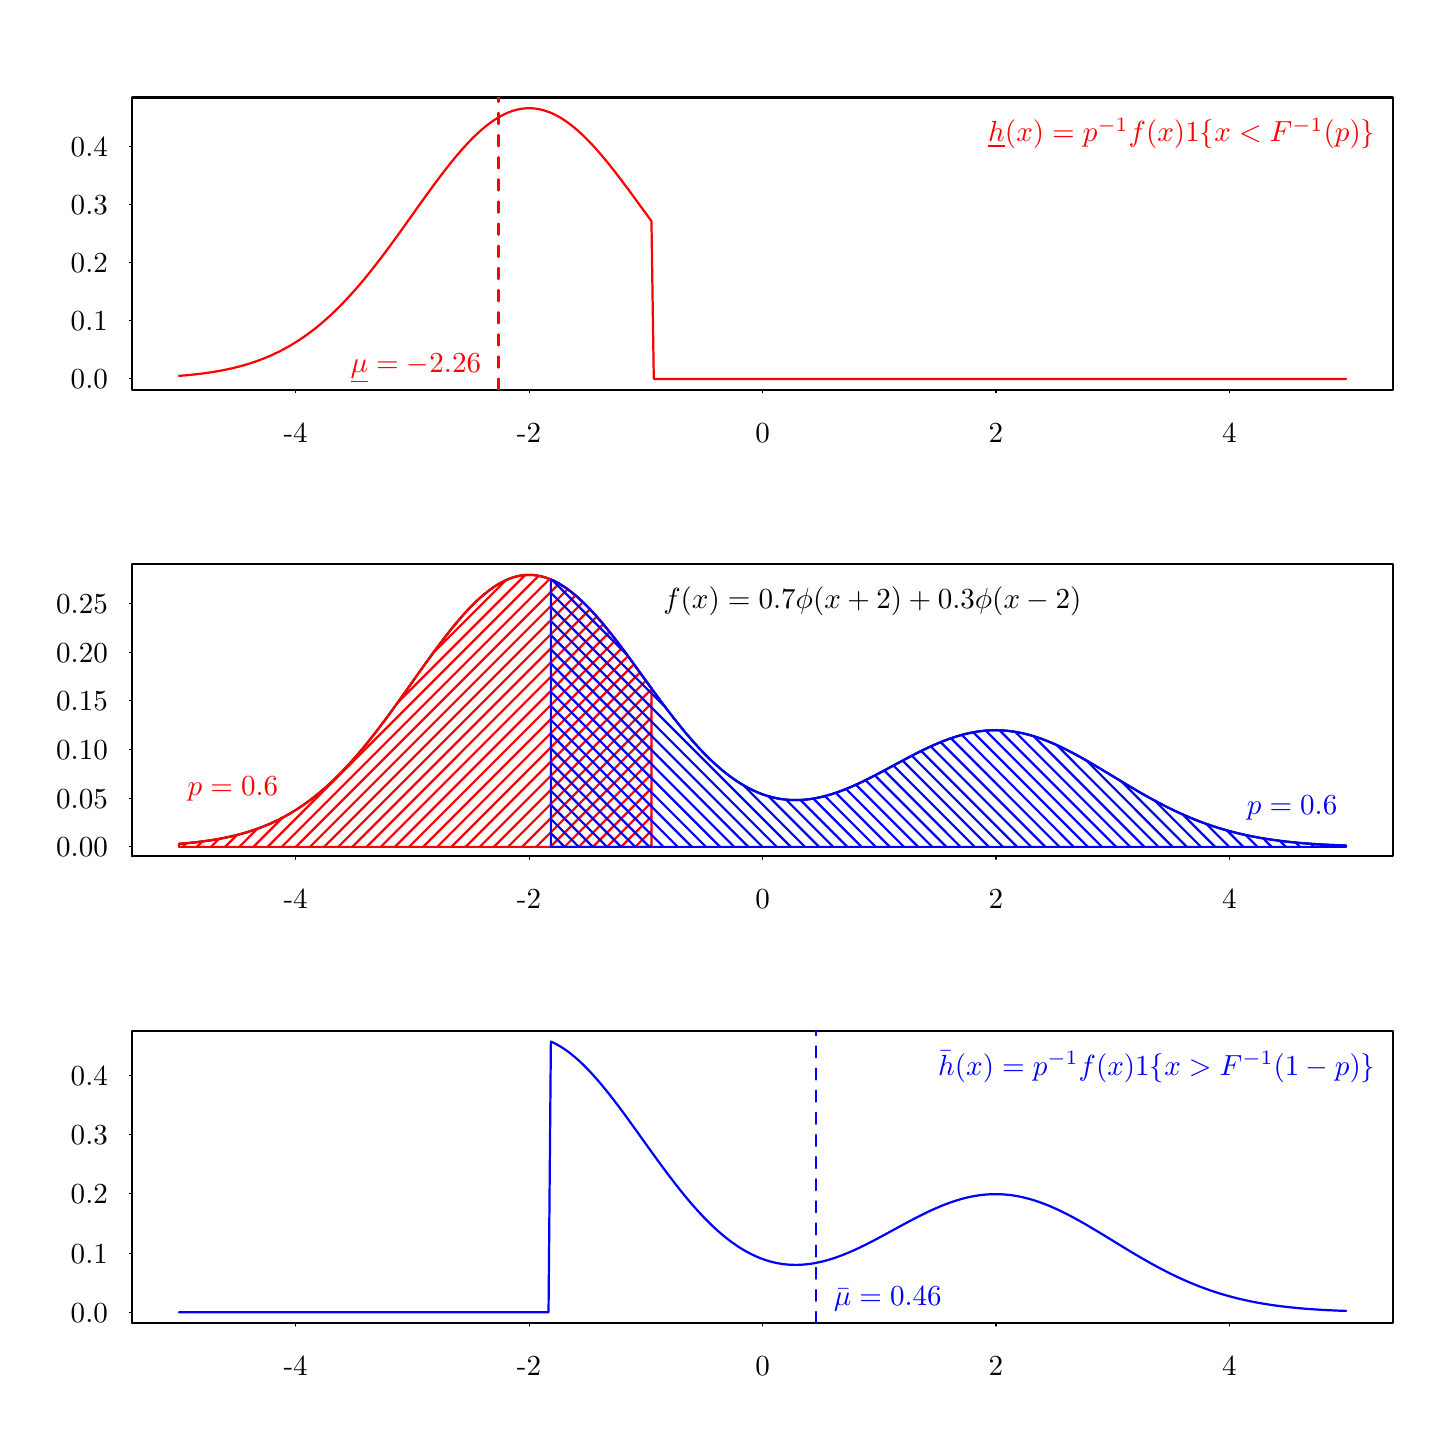
\begin{tikzpicture}[x=1pt,y=1pt]
\definecolor{fillColor}{RGB}{255,255,255}
\path[use as bounding box,fill=fillColor,fill opacity=0.00] (0,0) rectangle (505.89,505.89);
\begin{scope}
\path[clip] ( 37.80,375.06) rectangle (493.29,480.69);
\definecolor{drawColor}{RGB}{255,0,0}

\path[draw=drawColor,line width= 0.8pt,line join=round,line cap=round] ( 54.67,380.06) --
	( 55.52,380.13) --
	( 56.36,380.20) --
	( 57.21,380.27) --
	( 58.05,380.35) --
	( 58.90,380.43) --
	( 59.74,380.52) --
	( 60.59,380.61) --
	( 61.43,380.71) --
	( 62.28,380.81) --
	( 63.12,380.91) --
	( 63.97,381.03) --
	( 64.81,381.14) --
	( 65.66,381.27) --
	( 66.50,381.40) --
	( 67.35,381.53) --
	( 68.19,381.67) --
	( 69.04,381.82) --
	( 69.88,381.98) --
	( 70.73,382.14) --
	( 71.57,382.31) --
	( 72.42,382.49) --
	( 73.26,382.67) --
	( 74.11,382.87) --
	( 74.95,383.07) --
	( 75.80,383.28) --
	( 76.64,383.50) --
	( 77.49,383.73) --
	( 78.34,383.97) --
	( 79.18,384.22) --
	( 80.03,384.48) --
	( 80.87,384.75) --
	( 81.72,385.03) --
	( 82.56,385.32) --
	( 83.41,385.62) --
	( 84.25,385.94) --
	( 85.10,386.27) --
	( 85.94,386.60) --
	( 86.79,386.96) --
	( 87.63,387.32) --
	( 88.48,387.70) --
	( 89.32,388.09) --
	( 90.17,388.50) --
	( 91.01,388.91) --
	( 91.86,389.35) --
	( 92.70,389.79) --
	( 93.55,390.26) --
	( 94.39,390.73) --
	( 95.24,391.23) --
	( 96.08,391.74) --
	( 96.93,392.26) --
	( 97.77,392.80) --
	( 98.62,393.36) --
	( 99.47,393.93) --
	(100.31,394.52) --
	(101.16,395.12) --
	(102.00,395.75) --
	(102.85,396.39) --
	(103.69,397.04) --
	(104.54,397.72) --
	(105.38,398.41) --
	(106.23,399.12) --
	(107.07,399.84) --
	(107.92,400.59) --
	(108.76,401.35) --
	(109.61,402.13) --
	(110.45,402.93) --
	(111.30,403.74) --
	(112.14,404.57) --
	(112.99,405.42) --
	(113.83,406.28) --
	(114.68,407.17) --
	(115.52,408.07) --
	(116.37,408.98) --
	(117.21,409.92) --
	(118.06,410.86) --
	(118.90,411.83) --
	(119.75,412.81) --
	(120.59,413.80) --
	(121.44,414.82) --
	(122.29,415.84) --
	(123.13,416.88) --
	(123.98,417.93) --
	(124.82,419.00) --
	(125.67,420.08) --
	(126.51,421.17) --
	(127.36,422.27) --
	(128.20,423.38) --
	(129.05,424.50) --
	(129.89,425.64) --
	(130.74,426.78) --
	(131.58,427.93) --
	(132.43,429.09) --
	(133.27,430.25) --
	(134.12,431.42) --
	(134.96,432.60) --
	(135.81,433.78) --
	(136.65,434.96) --
	(137.50,436.15) --
	(138.34,437.34) --
	(139.19,438.52) --
	(140.03,439.71) --
	(140.88,440.90) --
	(141.72,442.09) --
	(142.57,443.27) --
	(143.41,444.45) --
	(144.26,445.62) --
	(145.11,446.78) --
	(145.95,447.94) --
	(146.80,449.09) --
	(147.64,450.24) --
	(148.49,451.37) --
	(149.33,452.49) --
	(150.18,453.59) --
	(151.02,454.68) --
	(151.87,455.76) --
	(152.71,456.82) --
	(153.56,457.87) --
	(154.40,458.90) --
	(155.25,459.90) --
	(156.09,460.89) --
	(156.94,461.86) --
	(157.78,462.80) --
	(158.63,463.72) --
	(159.47,464.62) --
	(160.32,465.49) --
	(161.16,466.34) --
	(162.01,467.15) --
	(162.85,467.94) --
	(163.70,468.71) --
	(164.54,469.44) --
	(165.39,470.14) --
	(166.24,470.81) --
	(167.08,471.44) --
	(167.93,472.05) --
	(168.77,472.62) --
	(169.62,473.15) --
	(170.46,473.65) --
	(171.31,474.12) --
	(172.15,474.55) --
	(173.00,474.94) --
	(173.84,475.30) --
	(174.69,475.62) --
	(175.53,475.90) --
	(176.38,476.14) --
	(177.22,476.34) --
	(178.07,476.51) --
	(178.91,476.63) --
	(179.76,476.72) --
	(180.60,476.77) --
	(181.45,476.78) --
	(182.29,476.75) --
	(183.14,476.68) --
	(183.98,476.57) --
	(184.83,476.42) --
	(185.67,476.24) --
	(186.52,476.01) --
	(187.36,475.75) --
	(188.21,475.45) --
	(189.06,475.11) --
	(189.90,474.74) --
	(190.75,474.32) --
	(191.59,473.88) --
	(192.44,473.39) --
	(193.28,472.87) --
	(194.13,472.32) --
	(194.97,471.73) --
	(195.82,471.11) --
	(196.66,470.46) --
	(197.51,469.78) --
	(198.35,469.06) --
	(199.20,468.32) --
	(200.04,467.55) --
	(200.89,466.75) --
	(201.73,465.92) --
	(202.58,465.06) --
	(203.42,464.18) --
	(204.27,463.28) --
	(205.11,462.35) --
	(205.96,461.40) --
	(206.80,460.43) --
	(207.65,459.44) --
	(208.49,458.43) --
	(209.34,457.41) --
	(210.19,456.36) --
	(211.03,455.30) --
	(211.88,454.23) --
	(212.72,453.14) --
	(213.57,452.04) --
	(214.41,450.93) --
	(215.26,449.81) --
	(216.10,448.68) --
	(216.95,447.54) --
	(217.79,446.40) --
	(218.64,445.24) --
	(219.48,444.09) --
	(220.33,442.93) --
	(221.17,441.77) --
	(222.02,440.61) --
	(222.86,439.45) --
	(223.71,438.29) --
	(224.55,437.13) --
	(225.40,435.97) --
	(226.24,378.97) --
	(227.09,378.97) --
	(227.93,378.97) --
	(228.78,378.97) --
	(229.62,378.97) --
	(230.47,378.97) --
	(231.31,378.97) --
	(232.16,378.97) --
	(233.01,378.97) --
	(233.85,378.97) --
	(234.70,378.97) --
	(235.54,378.97) --
	(236.39,378.97) --
	(237.23,378.97) --
	(238.08,378.97) --
	(238.92,378.97) --
	(239.77,378.97) --
	(240.61,378.97) --
	(241.46,378.97) --
	(242.30,378.97) --
	(243.15,378.97) --
	(243.99,378.97) --
	(244.84,378.97) --
	(245.68,378.97) --
	(246.53,378.97) --
	(247.37,378.97) --
	(248.22,378.97) --
	(249.06,378.97) --
	(249.91,378.97) --
	(250.75,378.97) --
	(251.60,378.97) --
	(252.44,378.97) --
	(253.29,378.97) --
	(254.13,378.97) --
	(254.98,378.97) --
	(255.83,378.97) --
	(256.67,378.97) --
	(257.52,378.97) --
	(258.36,378.97) --
	(259.21,378.97) --
	(260.05,378.97) --
	(260.90,378.97) --
	(261.74,378.97) --
	(262.59,378.97) --
	(263.43,378.97) --
	(264.28,378.97) --
	(265.12,378.97) --
	(265.97,378.97) --
	(266.81,378.97) --
	(267.66,378.97) --
	(268.50,378.97) --
	(269.35,378.97) --
	(270.19,378.97) --
	(271.04,378.97) --
	(271.88,378.97) --
	(272.73,378.97) --
	(273.57,378.97) --
	(274.42,378.97) --
	(275.26,378.97) --
	(276.11,378.97) --
	(276.96,378.97) --
	(277.80,378.97) --
	(278.65,378.97) --
	(279.49,378.97) --
	(280.34,378.97) --
	(281.18,378.97) --
	(282.03,378.97) --
	(282.87,378.97) --
	(283.72,378.97) --
	(284.56,378.97) --
	(285.41,378.97) --
	(286.25,378.97) --
	(287.10,378.97) --
	(287.94,378.97) --
	(288.79,378.97) --
	(289.63,378.97) --
	(290.48,378.97) --
	(291.32,378.97) --
	(292.17,378.97) --
	(293.01,378.97) --
	(293.86,378.97) --
	(294.70,378.97) --
	(295.55,378.97) --
	(296.39,378.97) --
	(297.24,378.97) --
	(298.08,378.97) --
	(298.93,378.97) --
	(299.78,378.97) --
	(300.62,378.97) --
	(301.47,378.97) --
	(302.31,378.97) --
	(303.16,378.97) --
	(304.00,378.97) --
	(304.85,378.97) --
	(305.69,378.97) --
	(306.54,378.97) --
	(307.38,378.97) --
	(308.23,378.97) --
	(309.07,378.97) --
	(309.92,378.97) --
	(310.76,378.97) --
	(311.61,378.97) --
	(312.45,378.97) --
	(313.30,378.97) --
	(314.14,378.97) --
	(314.99,378.97) --
	(315.83,378.97) --
	(316.68,378.97) --
	(317.52,378.97) --
	(318.37,378.97) --
	(319.21,378.97) --
	(320.06,378.97) --
	(320.90,378.97) --
	(321.75,378.97) --
	(322.60,378.97) --
	(323.44,378.97) --
	(324.29,378.97) --
	(325.13,378.97) --
	(325.98,378.97) --
	(326.82,378.97) --
	(327.67,378.97) --
	(328.51,378.97) --
	(329.36,378.97) --
	(330.20,378.97) --
	(331.05,378.97) --
	(331.89,378.97) --
	(332.74,378.97) --
	(333.58,378.97) --
	(334.43,378.97) --
	(335.27,378.97) --
	(336.12,378.97) --
	(336.96,378.97) --
	(337.81,378.97) --
	(338.65,378.97) --
	(339.50,378.97) --
	(340.34,378.97) --
	(341.19,378.97) --
	(342.03,378.97) --
	(342.88,378.97) --
	(343.73,378.97) --
	(344.57,378.97) --
	(345.42,378.97) --
	(346.26,378.97) --
	(347.11,378.97) --
	(347.95,378.97) --
	(348.80,378.97) --
	(349.64,378.97) --
	(350.49,378.97) --
	(351.33,378.97) --
	(352.18,378.97) --
	(353.02,378.97) --
	(353.87,378.97) --
	(354.71,378.97) --
	(355.56,378.97) --
	(356.40,378.97) --
	(357.25,378.97) --
	(358.09,378.97) --
	(358.94,378.97) --
	(359.78,378.97) --
	(360.63,378.97) --
	(361.47,378.97) --
	(362.32,378.97) --
	(363.16,378.97) --
	(364.01,378.97) --
	(364.85,378.97) --
	(365.70,378.97) --
	(366.55,378.97) --
	(367.39,378.97) --
	(368.24,378.97) --
	(369.08,378.97) --
	(369.93,378.97) --
	(370.77,378.97) --
	(371.62,378.97) --
	(372.46,378.97) --
	(373.31,378.97) --
	(374.15,378.97) --
	(375.00,378.97) --
	(375.84,378.97) --
	(376.69,378.97) --
	(377.53,378.97) --
	(378.38,378.97) --
	(379.22,378.97) --
	(380.07,378.97) --
	(380.91,378.97) --
	(381.76,378.97) --
	(382.60,378.97) --
	(383.45,378.97) --
	(384.29,378.97) --
	(385.14,378.97) --
	(385.98,378.97) --
	(386.83,378.97) --
	(387.68,378.97) --
	(388.52,378.97) --
	(389.37,378.97) --
	(390.21,378.97) --
	(391.06,378.97) --
	(391.90,378.97) --
	(392.75,378.97) --
	(393.59,378.97) --
	(394.44,378.97) --
	(395.28,378.97) --
	(396.13,378.97) --
	(396.97,378.97) --
	(397.82,378.97) --
	(398.66,378.97) --
	(399.51,378.97) --
	(400.35,378.97) --
	(401.20,378.97) --
	(402.04,378.97) --
	(402.89,378.97) --
	(403.73,378.97) --
	(404.58,378.97) --
	(405.42,378.97) --
	(406.27,378.97) --
	(407.11,378.97) --
	(407.96,378.97) --
	(408.80,378.97) --
	(409.65,378.97) --
	(410.50,378.97) --
	(411.34,378.97) --
	(412.19,378.97) --
	(413.03,378.97) --
	(413.88,378.97) --
	(414.72,378.97) --
	(415.57,378.97) --
	(416.41,378.97) --
	(417.26,378.97) --
	(418.10,378.97) --
	(418.95,378.97) --
	(419.79,378.97) --
	(420.64,378.97) --
	(421.48,378.97) --
	(422.33,378.97) --
	(423.17,378.97) --
	(424.02,378.97) --
	(424.86,378.97) --
	(425.71,378.97) --
	(426.55,378.97) --
	(427.40,378.97) --
	(428.24,378.97) --
	(429.09,378.97) --
	(429.93,378.97) --
	(430.78,378.97) --
	(431.62,378.97) --
	(432.47,378.97) --
	(433.32,378.97) --
	(434.16,378.97) --
	(435.01,378.97) --
	(435.85,378.97) --
	(436.70,378.97) --
	(437.54,378.97) --
	(438.39,378.97) --
	(439.23,378.97) --
	(440.08,378.97) --
	(440.92,378.97) --
	(441.77,378.97) --
	(442.61,378.97) --
	(443.46,378.97) --
	(444.30,378.97) --
	(445.15,378.97) --
	(445.99,378.97) --
	(446.84,378.97) --
	(447.68,378.97) --
	(448.53,378.97) --
	(449.37,378.97) --
	(450.22,378.97) --
	(451.06,378.97) --
	(451.91,378.97) --
	(452.75,378.97) --
	(453.60,378.97) --
	(454.45,378.97) --
	(455.29,378.97) --
	(456.14,378.97) --
	(456.98,378.97) --
	(457.83,378.97) --
	(458.67,378.97) --
	(459.52,378.97) --
	(460.36,378.97) --
	(461.21,378.97) --
	(462.05,378.97) --
	(462.90,378.97) --
	(463.74,378.97) --
	(464.59,378.97) --
	(465.43,378.97) --
	(466.28,378.97) --
	(467.12,378.97) --
	(467.97,378.97) --
	(468.81,378.97) --
	(469.66,378.97) --
	(470.50,378.97) --
	(471.35,378.97) --
	(472.19,378.97) --
	(473.04,378.97) --
	(473.88,378.97) --
	(474.73,378.97) --
	(475.57,378.97) --
	(476.42,378.97);
\end{scope}
\begin{scope}
\path[clip] (  0.00,  0.00) rectangle (505.89,505.89);
\definecolor{drawColor}{RGB}{0,0,0}

\path[draw=drawColor,line width= 0.4pt,line join=round,line cap=round] ( 96.84,375.06) -- (434.25,375.06);

\path[draw=drawColor,line width= 0.4pt,line join=round,line cap=round] ( 96.84,375.06) -- ( 96.84,374.00);

\path[draw=drawColor,line width= 0.4pt,line join=round,line cap=round] (181.19,375.06) -- (181.19,374.00);

\path[draw=drawColor,line width= 0.4pt,line join=round,line cap=round] (265.54,375.06) -- (265.54,374.00);

\path[draw=drawColor,line width= 0.4pt,line join=round,line cap=round] (349.89,375.06) -- (349.89,374.00);

\path[draw=drawColor,line width= 0.4pt,line join=round,line cap=round] (434.25,375.06) -- (434.25,374.00);

\node[text=drawColor,anchor=base,inner sep=0pt, outer sep=0pt, scale=  1.05] at ( 96.84,356.16) {-4};

\node[text=drawColor,anchor=base,inner sep=0pt, outer sep=0pt, scale=  1.05] at (181.19,356.16) {-2};

\node[text=drawColor,anchor=base,inner sep=0pt, outer sep=0pt, scale=  1.05] at (265.54,356.16) {0};

\node[text=drawColor,anchor=base,inner sep=0pt, outer sep=0pt, scale=  1.05] at (349.89,356.16) {2};

\node[text=drawColor,anchor=base,inner sep=0pt, outer sep=0pt, scale=  1.05] at (434.25,356.16) {4};

\path[draw=drawColor,line width= 0.4pt,line join=round,line cap=round] ( 37.80,378.97) -- ( 37.80,463.02);

\path[draw=drawColor,line width= 0.4pt,line join=round,line cap=round] ( 37.80,378.97) -- ( 36.74,378.97);

\path[draw=drawColor,line width= 0.4pt,line join=round,line cap=round] ( 37.80,399.98) -- ( 36.74,399.98);

\path[draw=drawColor,line width= 0.4pt,line join=round,line cap=round] ( 37.80,420.99) -- ( 36.74,420.99);

\path[draw=drawColor,line width= 0.4pt,line join=round,line cap=round] ( 37.80,442.01) -- ( 36.74,442.01);

\path[draw=drawColor,line width= 0.4pt,line join=round,line cap=round] ( 37.80,463.02) -- ( 36.74,463.02);

\node[text=drawColor,anchor=base east,inner sep=0pt, outer sep=0pt, scale=  1.05] at ( 28.98,375.36) {0.0};

\node[text=drawColor,anchor=base east,inner sep=0pt, outer sep=0pt, scale=  1.05] at ( 28.98,396.37) {0.1};

\node[text=drawColor,anchor=base east,inner sep=0pt, outer sep=0pt, scale=  1.05] at ( 28.98,417.38) {0.2};

\node[text=drawColor,anchor=base east,inner sep=0pt, outer sep=0pt, scale=  1.05] at ( 28.98,438.39) {0.3};

\node[text=drawColor,anchor=base east,inner sep=0pt, outer sep=0pt, scale=  1.05] at ( 28.98,459.40) {0.4};

\path[draw=drawColor,line width= 0.8pt,line join=round,line cap=round] ( 37.80,375.06) --
	(493.29,375.06) --
	(493.29,480.69) --
	( 37.80,480.69) --
	( 37.80,375.06);
\end{scope}
\begin{scope}
\path[clip] ( 37.80,375.06) rectangle (493.29,480.69);
\definecolor{drawColor}{RGB}{255,0,0}

\node[text=drawColor,anchor=base east,inner sep=0pt, outer sep=0pt, scale=  1.05] at (486.99,464.59) {$\underline{h}(x) = p^{-1}f(x) 1\{x < F^{-1}(p)\}$};

\path[draw=drawColor,line width= 0.8pt,dash pattern=on 4pt off 4pt ,line join=round,line cap=round] (170.15,375.06) -- (170.15,480.69);

\node[text=drawColor,anchor=base east,inner sep=0pt, outer sep=0pt, scale=  1.05] at (163.85,381.45) {$\underline{\mu} = -2.26$};
\end{scope}
\begin{scope}
\path[clip] ( 37.80,206.43) rectangle (493.29,312.06);
\definecolor{drawColor}{RGB}{0,0,0}

\path[draw=drawColor,line width= 0.8pt,line join=round,line cap=round] ( 54.67,210.97) --
	( 55.52,211.03) --
	( 56.36,211.10) --
	( 57.21,211.18) --
	( 58.05,211.26) --
	( 58.90,211.34) --
	( 59.74,211.43) --
	( 60.59,211.52) --
	( 61.43,211.62) --
	( 62.28,211.72) --
	( 63.12,211.83) --
	( 63.97,211.94) --
	( 64.81,212.06) --
	( 65.66,212.18) --
	( 66.50,212.31) --
	( 67.35,212.45) --
	( 68.19,212.59) --
	( 69.04,212.74) --
	( 69.88,212.89) --
	( 70.73,213.06) --
	( 71.57,213.23) --
	( 72.42,213.41) --
	( 73.26,213.59) --
	( 74.11,213.79) --
	( 74.95,213.99) --
	( 75.80,214.20) --
	( 76.64,214.42) --
	( 77.49,214.65) --
	( 78.34,214.90) --
	( 79.18,215.15) --
	( 80.03,215.41) --
	( 80.87,215.68) --
	( 81.72,215.96) --
	( 82.56,216.25) --
	( 83.41,216.56) --
	( 84.25,216.87) --
	( 85.10,217.20) --
	( 85.94,217.54) --
	( 86.79,217.90) --
	( 87.63,218.26) --
	( 88.48,218.64) --
	( 89.32,219.04) --
	( 90.17,219.44) --
	( 91.01,219.86) --
	( 91.86,220.30) --
	( 92.70,220.75) --
	( 93.55,221.21) --
	( 94.39,221.69) --
	( 95.24,222.19) --
	( 96.08,222.70) --
	( 96.93,223.23) --
	( 97.77,223.77) --
	( 98.62,224.33) --
	( 99.47,224.90) --
	(100.31,225.49) --
	(101.16,226.10) --
	(102.00,226.73) --
	(102.85,227.37) --
	(103.69,228.03) --
	(104.54,228.71) --
	(105.38,229.40) --
	(106.23,230.12) --
	(107.07,230.85) --
	(107.92,231.59) --
	(108.76,232.36) --
	(109.61,233.14) --
	(110.45,233.94) --
	(111.30,234.76) --
	(112.14,235.59) --
	(112.99,236.45) --
	(113.83,237.32) --
	(114.68,238.20) --
	(115.52,239.11) --
	(116.37,240.03) --
	(117.21,240.97) --
	(118.06,241.92) --
	(118.90,242.89) --
	(119.75,243.87) --
	(120.59,244.87) --
	(121.44,245.89) --
	(122.29,246.92) --
	(123.13,247.96) --
	(123.98,249.02) --
	(124.82,250.09) --
	(125.67,251.17) --
	(126.51,252.27) --
	(127.36,253.38) --
	(128.20,254.50) --
	(129.05,255.62) --
	(129.89,256.76) --
	(130.74,257.91) --
	(131.58,259.07) --
	(132.43,260.23) --
	(133.27,261.40) --
	(134.12,262.58) --
	(134.96,263.76) --
	(135.81,264.94) --
	(136.65,266.13) --
	(137.50,267.32) --
	(138.34,268.52) --
	(139.19,269.71) --
	(140.03,270.91) --
	(140.88,272.10) --
	(141.72,273.29) --
	(142.57,274.48) --
	(143.41,275.66) --
	(144.26,276.84) --
	(145.11,278.01) --
	(145.95,279.18) --
	(146.80,280.33) --
	(147.64,281.48) --
	(148.49,282.61) --
	(149.33,283.74) --
	(150.18,284.85) --
	(151.02,285.95) --
	(151.87,287.03) --
	(152.71,288.10) --
	(153.56,289.15) --
	(154.40,290.18) --
	(155.25,291.19) --
	(156.09,292.19) --
	(156.94,293.16) --
	(157.78,294.11) --
	(158.63,295.03) --
	(159.47,295.93) --
	(160.32,296.81) --
	(161.16,297.66) --
	(162.01,298.48) --
	(162.85,299.27) --
	(163.70,300.04) --
	(164.54,300.77) --
	(165.39,301.47) --
	(166.24,302.15) --
	(167.08,302.79) --
	(167.93,303.39) --
	(168.77,303.97) --
	(169.62,304.51) --
	(170.46,305.01) --
	(171.31,305.48) --
	(172.15,305.91) --
	(173.00,306.30) --
	(173.84,306.66) --
	(174.69,306.98) --
	(175.53,307.26) --
	(176.38,307.50) --
	(177.22,307.71) --
	(178.07,307.88) --
	(178.91,308.00) --
	(179.76,308.09) --
	(180.60,308.14) --
	(181.45,308.15) --
	(182.29,308.12) --
	(183.14,308.05) --
	(183.98,307.94) --
	(184.83,307.79) --
	(185.67,307.60) --
	(186.52,307.38) --
	(187.36,307.11) --
	(188.21,306.81) --
	(189.06,306.47) --
	(189.90,306.10) --
	(190.75,305.68) --
	(191.59,305.23) --
	(192.44,304.75) --
	(193.28,304.22) --
	(194.13,303.67) --
	(194.97,303.08) --
	(195.82,302.46) --
	(196.66,301.80) --
	(197.51,301.12) --
	(198.35,300.40) --
	(199.20,299.65) --
	(200.04,298.87) --
	(200.89,298.07) --
	(201.73,297.24) --
	(202.58,296.38) --
	(203.42,295.49) --
	(204.27,294.59) --
	(205.11,293.65) --
	(205.96,292.70) --
	(206.80,291.73) --
	(207.65,290.73) --
	(208.49,289.72) --
	(209.34,288.68) --
	(210.19,287.63) --
	(211.03,286.57) --
	(211.88,285.49) --
	(212.72,284.40) --
	(213.57,283.29) --
	(214.41,282.18) --
	(215.26,281.05) --
	(216.10,279.91) --
	(216.95,278.77) --
	(217.79,277.62) --
	(218.64,276.46) --
	(219.48,275.30) --
	(220.33,274.14) --
	(221.17,272.97) --
	(222.02,271.81) --
	(222.86,270.64) --
	(223.71,269.47) --
	(224.55,268.31) --
	(225.40,267.15) --
	(226.24,265.99) --
	(227.09,264.84) --
	(227.93,263.69) --
	(228.78,262.55) --
	(229.62,261.42) --
	(230.47,260.29) --
	(231.31,259.18) --
	(232.16,258.08) --
	(233.01,256.98) --
	(233.85,255.90) --
	(234.70,254.83) --
	(235.54,253.78) --
	(236.39,252.74) --
	(237.23,251.71) --
	(238.08,250.70) --
	(238.92,249.71) --
	(239.77,248.73) --
	(240.61,247.77) --
	(241.46,246.82) --
	(242.30,245.90) --
	(243.15,244.99) --
	(243.99,244.10) --
	(244.84,243.24) --
	(245.68,242.39) --
	(246.53,241.56) --
	(247.37,240.76) --
	(248.22,239.97) --
	(249.06,239.21) --
	(249.91,238.47) --
	(250.75,237.75) --
	(251.60,237.05) --
	(252.44,236.38) --
	(253.29,235.73) --
	(254.13,235.10) --
	(254.98,234.49) --
	(255.83,233.91) --
	(256.67,233.35) --
	(257.52,232.81) --
	(258.36,232.30) --
	(259.21,231.81) --
	(260.05,231.34) --
	(260.90,230.90) --
	(261.74,230.48) --
	(262.59,230.08) --
	(263.43,229.70) --
	(264.28,229.35) --
	(265.12,229.03) --
	(265.97,228.72) --
	(266.81,228.44) --
	(267.66,228.18) --
	(268.50,227.94) --
	(269.35,227.73) --
	(270.19,227.54) --
	(271.04,227.37) --
	(271.88,227.22) --
	(272.73,227.09) --
	(273.57,226.99) --
	(274.42,226.90) --
	(275.26,226.84) --
	(276.11,226.80) --
	(276.96,226.78) --
	(277.80,226.77) --
	(278.65,226.79) --
	(279.49,226.83) --
	(280.34,226.88) --
	(281.18,226.96) --
	(282.03,227.05) --
	(282.87,227.16) --
	(283.72,227.29) --
	(284.56,227.44) --
	(285.41,227.60) --
	(286.25,227.78) --
	(287.10,227.97) --
	(287.94,228.18) --
	(288.79,228.41) --
	(289.63,228.65) --
	(290.48,228.91) --
	(291.32,229.18) --
	(292.17,229.46) --
	(293.01,229.76) --
	(293.86,230.07) --
	(294.70,230.39) --
	(295.55,230.72) --
	(296.39,231.07) --
	(297.24,231.42) --
	(298.08,231.79) --
	(298.93,232.16) --
	(299.78,232.55) --
	(300.62,232.94) --
	(301.47,233.34) --
	(302.31,233.75) --
	(303.16,234.16) --
	(304.00,234.59) --
	(304.85,235.01) --
	(305.69,235.45) --
	(306.54,235.89) --
	(307.38,236.33) --
	(308.23,236.78) --
	(309.07,237.23) --
	(309.92,237.68) --
	(310.76,238.13) --
	(311.61,238.59) --
	(312.45,239.05) --
	(313.30,239.50) --
	(314.14,239.96) --
	(314.99,240.41) --
	(315.83,240.87) --
	(316.68,241.32) --
	(317.52,241.77) --
	(318.37,242.22) --
	(319.21,242.66) --
	(320.06,243.10) --
	(320.90,243.53) --
	(321.75,243.96) --
	(322.60,244.38) --
	(323.44,244.80) --
	(324.29,245.21) --
	(325.13,245.61) --
	(325.98,246.00) --
	(326.82,246.39) --
	(327.67,246.76) --
	(328.51,247.13) --
	(329.36,247.48) --
	(330.20,247.83) --
	(331.05,248.16) --
	(331.89,248.49) --
	(332.74,248.80) --
	(333.58,249.09) --
	(334.43,249.38) --
	(335.27,249.65) --
	(336.12,249.91) --
	(336.96,250.16) --
	(337.81,250.39) --
	(338.65,250.61) --
	(339.50,250.81) --
	(340.34,251.00) --
	(341.19,251.17) --
	(342.03,251.33) --
	(342.88,251.47) --
	(343.73,251.60) --
	(344.57,251.71) --
	(345.42,251.80) --
	(346.26,251.88) --
	(347.11,251.94) --
	(347.95,251.98) --
	(348.80,252.01) --
	(349.64,252.02) --
	(350.49,252.01) --
	(351.33,251.99) --
	(352.18,251.95) --
	(353.02,251.89) --
	(353.87,251.82) --
	(354.71,251.73) --
	(355.56,251.63) --
	(356.40,251.51) --
	(357.25,251.37) --
	(358.09,251.21) --
	(358.94,251.04) --
	(359.78,250.86) --
	(360.63,250.66) --
	(361.47,250.44) --
	(362.32,250.21) --
	(363.16,249.96) --
	(364.01,249.70) --
	(364.85,249.43) --
	(365.70,249.14) --
	(366.55,248.84) --
	(367.39,248.52) --
	(368.24,248.19) --
	(369.08,247.85) --
	(369.93,247.50) --
	(370.77,247.13) --
	(371.62,246.76) --
	(372.46,246.37) --
	(373.31,245.98) --
	(374.15,245.57) --
	(375.00,245.15) --
	(375.84,244.73) --
	(376.69,244.29) --
	(377.53,243.85) --
	(378.38,243.40) --
	(379.22,242.94) --
	(380.07,242.48) --
	(380.91,242.01) --
	(381.76,241.53) --
	(382.60,241.05) --
	(383.45,240.56) --
	(384.29,240.07) --
	(385.14,239.58) --
	(385.98,239.08) --
	(386.83,238.57) --
	(387.68,238.07) --
	(388.52,237.56) --
	(389.37,237.05) --
	(390.21,236.54) --
	(391.06,236.03) --
	(391.90,235.52) --
	(392.75,235.01) --
	(393.59,234.50) --
	(394.44,233.98) --
	(395.28,233.48) --
	(396.13,232.97) --
	(396.97,232.46) --
	(397.82,231.96) --
	(398.66,231.46) --
	(399.51,230.96) --
	(400.35,230.46) --
	(401.20,229.97) --
	(402.04,229.48) --
	(402.89,229.00) --
	(403.73,228.52) --
	(404.58,228.04) --
	(405.42,227.57) --
	(406.27,227.11) --
	(407.11,226.65) --
	(407.96,226.20) --
	(408.80,225.75) --
	(409.65,225.31) --
	(410.50,224.87) --
	(411.34,224.45) --
	(412.19,224.02) --
	(413.03,223.61) --
	(413.88,223.20) --
	(414.72,222.80) --
	(415.57,222.40) --
	(416.41,222.02) --
	(417.26,221.64) --
	(418.10,221.26) --
	(418.95,220.90) --
	(419.79,220.54) --
	(420.64,220.19) --
	(421.48,219.85) --
	(422.33,219.51) --
	(423.17,219.18) --
	(424.02,218.86) --
	(424.86,218.55) --
	(425.71,218.24) --
	(426.55,217.95) --
	(427.40,217.66) --
	(428.24,217.37) --
	(429.09,217.10) --
	(429.93,216.83) --
	(430.78,216.57) --
	(431.62,216.32) --
	(432.47,216.07) --
	(433.32,215.83) --
	(434.16,215.60) --
	(435.01,215.37) --
	(435.85,215.15) --
	(436.70,214.94) --
	(437.54,214.73) --
	(438.39,214.53) --
	(439.23,214.34) --
	(440.08,214.16) --
	(440.92,213.98) --
	(441.77,213.80) --
	(442.61,213.63) --
	(443.46,213.47) --
	(444.30,213.31) --
	(445.15,213.16) --
	(445.99,213.02) --
	(446.84,212.87) --
	(447.68,212.74) --
	(448.53,212.61) --
	(449.37,212.48) --
	(450.22,212.36) --
	(451.06,212.25) --
	(451.91,212.13) --
	(452.75,212.03) --
	(453.60,211.92) --
	(454.45,211.82) --
	(455.29,211.73) --
	(456.14,211.64) --
	(456.98,211.55) --
	(457.83,211.47) --
	(458.67,211.39) --
	(459.52,211.31) --
	(460.36,211.24) --
	(461.21,211.17) --
	(462.05,211.10) --
	(462.90,211.04) --
	(463.74,210.98) --
	(464.59,210.92) --
	(465.43,210.86) --
	(466.28,210.81) --
	(467.12,210.76) --
	(467.97,210.71) --
	(468.81,210.67) --
	(469.66,210.62) --
	(470.50,210.58) --
	(471.35,210.54) --
	(472.19,210.50) --
	(473.04,210.47) --
	(473.88,210.43) --
	(474.73,210.40) --
	(475.57,210.37) --
	(476.42,210.34);
\end{scope}
\begin{scope}
\path[clip] (  0.00,  0.00) rectangle (505.89,505.89);
\definecolor{drawColor}{RGB}{0,0,0}

\path[draw=drawColor,line width= 0.4pt,line join=round,line cap=round] ( 96.84,206.43) -- (434.25,206.43);

\path[draw=drawColor,line width= 0.4pt,line join=round,line cap=round] ( 96.84,206.43) -- ( 96.84,205.37);

\path[draw=drawColor,line width= 0.4pt,line join=round,line cap=round] (181.19,206.43) -- (181.19,205.37);

\path[draw=drawColor,line width= 0.4pt,line join=round,line cap=round] (265.54,206.43) -- (265.54,205.37);

\path[draw=drawColor,line width= 0.4pt,line join=round,line cap=round] (349.89,206.43) -- (349.89,205.37);

\path[draw=drawColor,line width= 0.4pt,line join=round,line cap=round] (434.25,206.43) -- (434.25,205.37);

\node[text=drawColor,anchor=base,inner sep=0pt, outer sep=0pt, scale=  1.05] at ( 96.84,187.53) {-4};

\node[text=drawColor,anchor=base,inner sep=0pt, outer sep=0pt, scale=  1.05] at (181.19,187.53) {-2};

\node[text=drawColor,anchor=base,inner sep=0pt, outer sep=0pt, scale=  1.05] at (265.54,187.53) {0};

\node[text=drawColor,anchor=base,inner sep=0pt, outer sep=0pt, scale=  1.05] at (349.89,187.53) {2};

\node[text=drawColor,anchor=base,inner sep=0pt, outer sep=0pt, scale=  1.05] at (434.25,187.53) {4};

\path[draw=drawColor,line width= 0.4pt,line join=round,line cap=round] ( 37.80,209.87) -- ( 37.80,297.84);

\path[draw=drawColor,line width= 0.4pt,line join=round,line cap=round] ( 37.80,209.87) -- ( 36.74,209.87);

\path[draw=drawColor,line width= 0.4pt,line join=round,line cap=round] ( 37.80,227.47) -- ( 36.74,227.47);

\path[draw=drawColor,line width= 0.4pt,line join=round,line cap=round] ( 37.80,245.06) -- ( 36.74,245.06);

\path[draw=drawColor,line width= 0.4pt,line join=round,line cap=round] ( 37.80,262.65) -- ( 36.74,262.65);

\path[draw=drawColor,line width= 0.4pt,line join=round,line cap=round] ( 37.80,280.25) -- ( 36.74,280.25);

\path[draw=drawColor,line width= 0.4pt,line join=round,line cap=round] ( 37.80,297.84) -- ( 36.74,297.84);

\node[text=drawColor,anchor=base east,inner sep=0pt, outer sep=0pt, scale=  1.05] at ( 28.98,206.26) {0.00};

\node[text=drawColor,anchor=base east,inner sep=0pt, outer sep=0pt, scale=  1.05] at ( 28.98,223.85) {0.05};

\node[text=drawColor,anchor=base east,inner sep=0pt, outer sep=0pt, scale=  1.05] at ( 28.98,241.44) {0.10};

\node[text=drawColor,anchor=base east,inner sep=0pt, outer sep=0pt, scale=  1.05] at ( 28.98,259.04) {0.15};

\node[text=drawColor,anchor=base east,inner sep=0pt, outer sep=0pt, scale=  1.05] at ( 28.98,276.63) {0.20};

\node[text=drawColor,anchor=base east,inner sep=0pt, outer sep=0pt, scale=  1.05] at ( 28.98,294.22) {0.25};

\path[draw=drawColor,line width= 0.8pt,line join=round,line cap=round] ( 37.80,206.43) --
	(493.29,206.43) --
	(493.29,312.06) --
	( 37.80,312.06) --
	( 37.80,206.43);
\end{scope}
\begin{scope}
\path[clip] ( 37.80,206.43) rectangle (493.29,312.06);
\definecolor{drawColor}{RGB}{255,0,0}

\path[draw=drawColor,line width= 0.8pt,line join=round,line cap=round] ( 56.02,209.87) -- ( 57.34,211.19);

\path[draw=drawColor,line width= 0.8pt,line join=round,line cap=round] ( 61.13,209.87) -- ( 63.08,211.82);

\path[draw=drawColor,line width= 0.8pt,line join=round,line cap=round] ( 66.24,209.87) -- ( 69.12,212.75);

\path[draw=drawColor,line width= 0.8pt,line join=round,line cap=round] ( 71.36,209.87) -- ( 75.64,214.16);

\path[draw=drawColor,line width= 0.8pt,line join=round,line cap=round] ( 76.47,209.87) -- ( 83.00,216.41);

\path[draw=drawColor,line width= 0.8pt,line join=round,line cap=round] (146.45,279.86) -- (172.80,306.21);

\path[draw=drawColor,line width= 0.8pt,line join=round,line cap=round] ( 81.58,209.87) -- ( 92.16,220.46);

\path[draw=drawColor,line width= 0.8pt,line join=round,line cap=round] (133.71,262.01) -- (179.79,308.09);

\path[draw=drawColor,line width= 0.8pt,line join=round,line cap=round] ( 86.69,209.87) -- (184.64,307.82);

\path[draw=drawColor,line width= 0.8pt,line join=round,line cap=round] ( 91.80,209.87) -- (188.58,306.66);

\path[draw=drawColor,line width= 0.8pt,line join=round,line cap=round] ( 96.91,209.87) -- (192.02,304.99);

\path[draw=drawColor,line width= 0.8pt,line join=round,line cap=round] (102.02,209.87) -- (195.12,302.97);

\path[draw=drawColor,line width= 0.8pt,line join=round,line cap=round] (107.13,209.87) -- (197.97,300.72);

\path[draw=drawColor,line width= 0.8pt,line join=round,line cap=round] (112.24,209.87) -- (200.65,298.29);

\path[draw=drawColor,line width= 0.8pt,line join=round,line cap=round] (117.35,209.87) -- (203.20,295.73);

\path[draw=drawColor,line width= 0.8pt,line join=round,line cap=round] (122.46,209.87) -- (205.64,293.06);

\path[draw=drawColor,line width= 0.8pt,line join=round,line cap=round] (127.57,209.87) -- (208.00,290.31);

\path[draw=drawColor,line width= 0.8pt,line join=round,line cap=round] (132.68,209.87) -- (210.30,287.49);

\path[draw=drawColor,line width= 0.8pt,line join=round,line cap=round] (137.79,209.87) -- (212.54,284.63);

\path[draw=drawColor,line width= 0.8pt,line join=round,line cap=round] (142.90,209.87) -- (214.75,281.72);

\path[draw=drawColor,line width= 0.8pt,line join=round,line cap=round] (148.01,209.87) -- (216.93,278.79);

\path[draw=drawColor,line width= 0.8pt,line join=round,line cap=round] (153.12,209.87) -- (219.09,275.84);

\path[draw=drawColor,line width= 0.8pt,line join=round,line cap=round] (158.23,209.87) -- (221.24,272.88);

\path[draw=drawColor,line width= 0.8pt,line join=round,line cap=round] (163.34,209.87) -- (223.39,269.92);

\path[draw=drawColor,line width= 0.8pt,line join=round,line cap=round] (168.45,209.87) -- (225.40,266.82);

\path[draw=drawColor,line width= 0.8pt,line join=round,line cap=round] (173.56,209.87) -- (225.40,261.71);

\path[draw=drawColor,line width= 0.8pt,line join=round,line cap=round] (178.67,209.87) -- (225.40,256.60);

\path[draw=drawColor,line width= 0.8pt,line join=round,line cap=round] (183.78,209.87) -- (225.40,251.49);

\path[draw=drawColor,line width= 0.8pt,line join=round,line cap=round] (188.89,209.87) -- (225.40,246.38);

\path[draw=drawColor,line width= 0.8pt,line join=round,line cap=round] (194.00,209.87) -- (225.40,241.27);

\path[draw=drawColor,line width= 0.8pt,line join=round,line cap=round] (199.11,209.87) -- (225.40,236.16);

\path[draw=drawColor,line width= 0.8pt,line join=round,line cap=round] (204.22,209.87) -- (225.40,231.05);

\path[draw=drawColor,line width= 0.8pt,line join=round,line cap=round] (209.33,209.87) -- (225.40,225.94);

\path[draw=drawColor,line width= 0.8pt,line join=round,line cap=round] (214.44,209.87) -- (225.40,220.83);

\path[draw=drawColor,line width= 0.8pt,line join=round,line cap=round] (219.55,209.87) -- (225.40,215.72);

\path[draw=drawColor,line width= 0.8pt,line join=round,line cap=round] (224.66,209.87) -- (225.40,210.61);

\path[draw=drawColor,line width= 0.8pt,line join=round,line cap=round] ( 54.67,209.87) --
	( 55.52,209.87) --
	( 56.36,209.87) --
	( 57.21,209.87) --
	( 58.05,209.87) --
	( 58.90,209.87) --
	( 59.74,209.87) --
	( 60.59,209.87) --
	( 61.43,209.87) --
	( 62.28,209.87) --
	( 63.12,209.87) --
	( 63.97,209.87) --
	( 64.81,209.87) --
	( 65.66,209.87) --
	( 66.50,209.87) --
	( 67.35,209.87) --
	( 68.19,209.87) --
	( 69.04,209.87) --
	( 69.88,209.87) --
	( 70.73,209.87) --
	( 71.57,209.87) --
	( 72.42,209.87) --
	( 73.26,209.87) --
	( 74.11,209.87) --
	( 74.95,209.87) --
	( 75.80,209.87) --
	( 76.64,209.87) --
	( 77.49,209.87) --
	( 78.34,209.87) --
	( 79.18,209.87) --
	( 80.03,209.87) --
	( 80.87,209.87) --
	( 81.72,209.87) --
	( 82.56,209.87) --
	( 83.41,209.87) --
	( 84.25,209.87) --
	( 85.10,209.87) --
	( 85.94,209.87) --
	( 86.79,209.87) --
	( 87.63,209.87) --
	( 88.48,209.87) --
	( 89.32,209.87) --
	( 90.17,209.87) --
	( 91.01,209.87) --
	( 91.86,209.87) --
	( 92.70,209.87) --
	( 93.55,209.87) --
	( 94.39,209.87) --
	( 95.24,209.87) --
	( 96.08,209.87) --
	( 96.93,209.87) --
	( 97.77,209.87) --
	( 98.62,209.87) --
	( 99.47,209.87) --
	(100.31,209.87) --
	(101.16,209.87) --
	(102.00,209.87) --
	(102.85,209.87) --
	(103.69,209.87) --
	(104.54,209.87) --
	(105.38,209.87) --
	(106.23,209.87) --
	(107.07,209.87) --
	(107.92,209.87) --
	(108.76,209.87) --
	(109.61,209.87) --
	(110.45,209.87) --
	(111.30,209.87) --
	(112.14,209.87) --
	(112.99,209.87) --
	(113.83,209.87) --
	(114.68,209.87) --
	(115.52,209.87) --
	(116.37,209.87) --
	(117.21,209.87) --
	(118.06,209.87) --
	(118.90,209.87) --
	(119.75,209.87) --
	(120.59,209.87) --
	(121.44,209.87) --
	(122.29,209.87) --
	(123.13,209.87) --
	(123.98,209.87) --
	(124.82,209.87) --
	(125.67,209.87) --
	(126.51,209.87) --
	(127.36,209.87) --
	(128.20,209.87) --
	(129.05,209.87) --
	(129.89,209.87) --
	(130.74,209.87) --
	(131.58,209.87) --
	(132.43,209.87) --
	(133.27,209.87) --
	(134.12,209.87) --
	(134.96,209.87) --
	(135.81,209.87) --
	(136.65,209.87) --
	(137.50,209.87) --
	(138.34,209.87) --
	(139.19,209.87) --
	(140.03,209.87) --
	(140.88,209.87) --
	(141.72,209.87) --
	(142.57,209.87) --
	(143.41,209.87) --
	(144.26,209.87) --
	(145.11,209.87) --
	(145.95,209.87) --
	(146.80,209.87) --
	(147.64,209.87) --
	(148.49,209.87) --
	(149.33,209.87) --
	(150.18,209.87) --
	(151.02,209.87) --
	(151.87,209.87) --
	(152.71,209.87) --
	(153.56,209.87) --
	(154.40,209.87) --
	(155.25,209.87) --
	(156.09,209.87) --
	(156.94,209.87) --
	(157.78,209.87) --
	(158.63,209.87) --
	(159.47,209.87) --
	(160.32,209.87) --
	(161.16,209.87) --
	(162.01,209.87) --
	(162.85,209.87) --
	(163.70,209.87) --
	(164.54,209.87) --
	(165.39,209.87) --
	(166.24,209.87) --
	(167.08,209.87) --
	(167.93,209.87) --
	(168.77,209.87) --
	(169.62,209.87) --
	(170.46,209.87) --
	(171.31,209.87) --
	(172.15,209.87) --
	(173.00,209.87) --
	(173.84,209.87) --
	(174.69,209.87) --
	(175.53,209.87) --
	(176.38,209.87) --
	(177.22,209.87) --
	(178.07,209.87) --
	(178.91,209.87) --
	(179.76,209.87) --
	(180.60,209.87) --
	(181.45,209.87) --
	(182.29,209.87) --
	(183.14,209.87) --
	(183.98,209.87) --
	(184.83,209.87) --
	(185.67,209.87) --
	(186.52,209.87) --
	(187.36,209.87) --
	(188.21,209.87) --
	(189.06,209.87) --
	(189.90,209.87) --
	(190.75,209.87) --
	(191.59,209.87) --
	(192.44,209.87) --
	(193.28,209.87) --
	(194.13,209.87) --
	(194.97,209.87) --
	(195.82,209.87) --
	(196.66,209.87) --
	(197.51,209.87) --
	(198.35,209.87) --
	(199.20,209.87) --
	(200.04,209.87) --
	(200.89,209.87) --
	(201.73,209.87) --
	(202.58,209.87) --
	(203.42,209.87) --
	(204.27,209.87) --
	(205.11,209.87) --
	(205.96,209.87) --
	(206.80,209.87) --
	(207.65,209.87) --
	(208.49,209.87) --
	(209.34,209.87) --
	(210.19,209.87) --
	(211.03,209.87) --
	(211.88,209.87) --
	(212.72,209.87) --
	(213.57,209.87) --
	(214.41,209.87) --
	(215.26,209.87) --
	(216.10,209.87) --
	(216.95,209.87) --
	(217.79,209.87) --
	(218.64,209.87) --
	(219.48,209.87) --
	(220.33,209.87) --
	(221.17,209.87) --
	(222.02,209.87) --
	(222.86,209.87) --
	(223.71,209.87) --
	(224.55,209.87) --
	(225.40,209.87) --
	(225.40,267.15) --
	(224.55,268.31) --
	(223.71,269.47) --
	(222.86,270.64) --
	(222.02,271.81) --
	(221.17,272.97) --
	(220.33,274.14) --
	(219.48,275.30) --
	(218.64,276.46) --
	(217.79,277.62) --
	(216.95,278.77) --
	(216.10,279.91) --
	(215.26,281.05) --
	(214.41,282.18) --
	(213.57,283.29) --
	(212.72,284.40) --
	(211.88,285.49) --
	(211.03,286.57) --
	(210.19,287.63) --
	(209.34,288.68) --
	(208.49,289.72) --
	(207.65,290.73) --
	(206.80,291.73) --
	(205.96,292.70) --
	(205.11,293.65) --
	(204.27,294.59) --
	(203.42,295.49) --
	(202.58,296.38) --
	(201.73,297.24) --
	(200.89,298.07) --
	(200.04,298.87) --
	(199.20,299.65) --
	(198.35,300.40) --
	(197.51,301.12) --
	(196.66,301.80) --
	(195.82,302.46) --
	(194.97,303.08) --
	(194.13,303.67) --
	(193.28,304.22) --
	(192.44,304.75) --
	(191.59,305.23) --
	(190.75,305.68) --
	(189.90,306.10) --
	(189.06,306.47) --
	(188.21,306.81) --
	(187.36,307.11) --
	(186.52,307.38) --
	(185.67,307.60) --
	(184.83,307.79) --
	(183.98,307.94) --
	(183.14,308.05) --
	(182.29,308.12) --
	(181.45,308.15) --
	(180.60,308.14) --
	(179.76,308.09) --
	(178.91,308.00) --
	(178.07,307.88) --
	(177.22,307.71) --
	(176.38,307.50) --
	(175.53,307.26) --
	(174.69,306.98) --
	(173.84,306.66) --
	(173.00,306.30) --
	(172.15,305.91) --
	(171.31,305.48) --
	(170.46,305.01) --
	(169.62,304.51) --
	(168.77,303.97) --
	(167.93,303.39) --
	(167.08,302.79) --
	(166.24,302.15) --
	(165.39,301.47) --
	(164.54,300.77) --
	(163.70,300.04) --
	(162.85,299.27) --
	(162.01,298.48) --
	(161.16,297.66) --
	(160.32,296.81) --
	(159.47,295.93) --
	(158.63,295.03) --
	(157.78,294.11) --
	(156.94,293.16) --
	(156.09,292.19) --
	(155.25,291.19) --
	(154.40,290.18) --
	(153.56,289.15) --
	(152.71,288.10) --
	(151.87,287.03) --
	(151.02,285.95) --
	(150.18,284.85) --
	(149.33,283.74) --
	(148.49,282.61) --
	(147.64,281.48) --
	(146.80,280.33) --
	(145.95,279.18) --
	(145.11,278.01) --
	(144.26,276.84) --
	(143.41,275.66) --
	(142.57,274.48) --
	(141.72,273.29) --
	(140.88,272.10) --
	(140.03,270.91) --
	(139.19,269.71) --
	(138.34,268.52) --
	(137.50,267.32) --
	(136.65,266.13) --
	(135.81,264.94) --
	(134.96,263.76) --
	(134.12,262.58) --
	(133.27,261.40) --
	(132.43,260.23) --
	(131.58,259.07) --
	(130.74,257.91) --
	(129.89,256.76) --
	(129.05,255.62) --
	(128.20,254.50) --
	(127.36,253.38) --
	(126.51,252.27) --
	(125.67,251.17) --
	(124.82,250.09) --
	(123.98,249.02) --
	(123.13,247.96) --
	(122.29,246.92) --
	(121.44,245.89) --
	(120.59,244.87) --
	(119.75,243.87) --
	(118.90,242.89) --
	(118.06,241.92) --
	(117.21,240.97) --
	(116.37,240.03) --
	(115.52,239.11) --
	(114.68,238.20) --
	(113.83,237.32) --
	(112.99,236.45) --
	(112.14,235.59) --
	(111.30,234.76) --
	(110.45,233.94) --
	(109.61,233.14) --
	(108.76,232.36) --
	(107.92,231.59) --
	(107.07,230.85) --
	(106.23,230.12) --
	(105.38,229.40) --
	(104.54,228.71) --
	(103.69,228.03) --
	(102.85,227.37) --
	(102.00,226.73) --
	(101.16,226.10) --
	(100.31,225.49) --
	( 99.47,224.90) --
	( 98.62,224.33) --
	( 97.77,223.77) --
	( 96.93,223.23) --
	( 96.08,222.70) --
	( 95.24,222.19) --
	( 94.39,221.69) --
	( 93.55,221.21) --
	( 92.70,220.75) --
	( 91.86,220.30) --
	( 91.01,219.86) --
	( 90.17,219.44) --
	( 89.32,219.04) --
	( 88.48,218.64) --
	( 87.63,218.26) --
	( 86.79,217.90) --
	( 85.94,217.54) --
	( 85.10,217.20) --
	( 84.25,216.87) --
	( 83.41,216.56) --
	( 82.56,216.25) --
	( 81.72,215.96) --
	( 80.87,215.68) --
	( 80.03,215.41) --
	( 79.18,215.15) --
	( 78.34,214.90) --
	( 77.49,214.65) --
	( 76.64,214.42) --
	( 75.80,214.20) --
	( 74.95,213.99) --
	( 74.11,213.79) --
	( 73.26,213.59) --
	( 72.42,213.41) --
	( 71.57,213.23) --
	( 70.73,213.06) --
	( 69.88,212.89) --
	( 69.04,212.74) --
	( 68.19,212.59) --
	( 67.35,212.45) --
	( 66.50,212.31) --
	( 65.66,212.18) --
	( 64.81,212.06) --
	( 63.97,211.94) --
	( 63.12,211.83) --
	( 62.28,211.72) --
	( 61.43,211.62) --
	( 60.59,211.52) --
	( 59.74,211.43) --
	( 58.90,211.34) --
	( 58.05,211.26) --
	( 57.21,211.18) --
	( 56.36,211.10) --
	( 55.52,211.03) --
	( 54.67,210.97) --
	( 54.67,209.87);

\node[text=drawColor,anchor=base east,inner sep=0pt, outer sep=0pt, scale=  1.05] at ( 90.54,228.58) {$p = 0.6$};
\definecolor{drawColor}{RGB}{0,0,255}

\path[draw=drawColor,line width= 0.8pt,line join=round,line cap=round] (194.00,209.87) -- (189.06,214.82);

\path[draw=drawColor,line width= 0.8pt,line join=round,line cap=round] (199.11,209.87) -- (189.06,219.93);

\path[draw=drawColor,line width= 0.8pt,line join=round,line cap=round] (204.22,209.87) -- (189.06,225.04);

\path[draw=drawColor,line width= 0.8pt,line join=round,line cap=round] (209.33,209.87) -- (189.06,230.15);

\path[draw=drawColor,line width= 0.8pt,line join=round,line cap=round] (214.44,209.87) -- (189.06,235.26);

\path[draw=drawColor,line width= 0.8pt,line join=round,line cap=round] (219.55,209.87) -- (189.06,240.37);

\path[draw=drawColor,line width= 0.8pt,line join=round,line cap=round] (224.66,209.87) -- (189.06,245.48);

\path[draw=drawColor,line width= 0.8pt,line join=round,line cap=round] (229.77,209.87) -- (189.06,250.59);

\path[draw=drawColor,line width= 0.8pt,line join=round,line cap=round] (234.88,209.87) -- (189.06,255.70);

\path[draw=drawColor,line width= 0.8pt,line join=round,line cap=round] (239.99,209.87) -- (189.06,260.81);

\path[draw=drawColor,line width= 0.8pt,line join=round,line cap=round] (245.10,209.87) -- (189.06,265.92);

\path[draw=drawColor,line width= 0.8pt,line join=round,line cap=round] (250.21,209.87) -- (189.06,271.03);

\path[draw=drawColor,line width= 0.8pt,line join=round,line cap=round] (255.32,209.87) -- (189.06,276.14);

\path[draw=drawColor,line width= 0.8pt,line join=round,line cap=round] (260.43,209.87) -- (189.06,281.25);

\path[draw=drawColor,line width= 0.8pt,line join=round,line cap=round] (265.54,209.87) -- (189.06,286.36);

\path[draw=drawColor,line width= 0.8pt,line join=round,line cap=round] (270.66,209.87) -- (189.06,291.47);

\path[draw=drawColor,line width= 0.8pt,line join=round,line cap=round] (275.77,209.87) -- (189.06,296.58);

\path[draw=drawColor,line width= 0.8pt,line join=round,line cap=round] (280.88,209.87) -- (258.58,232.17);

\path[draw=drawColor,line width= 0.8pt,line join=round,line cap=round] (230.51,260.24) -- (189.06,301.69);

\path[draw=drawColor,line width= 0.8pt,line join=round,line cap=round] (285.99,209.87) -- (267.69,228.17);

\path[draw=drawColor,line width= 0.8pt,line join=round,line cap=round] (216.54,279.32) -- (189.66,306.20);

\path[draw=drawColor,line width= 0.8pt,line join=round,line cap=round] (291.10,209.87) -- (274.03,226.94);

\path[draw=drawColor,line width= 0.8pt,line join=round,line cap=round] (296.21,209.87) -- (279.26,226.82);

\path[draw=drawColor,line width= 0.8pt,line join=round,line cap=round] (301.32,209.87) -- (283.87,227.32);

\path[draw=drawColor,line width= 0.8pt,line join=round,line cap=round] (306.43,209.87) -- (288.08,228.22);

\path[draw=drawColor,line width= 0.8pt,line join=round,line cap=round] (311.54,209.87) -- (292.01,229.41);

\path[draw=drawColor,line width= 0.8pt,line join=round,line cap=round] (316.65,209.87) -- (295.73,230.79);

\path[draw=drawColor,line width= 0.8pt,line join=round,line cap=round] (321.76,209.87) -- (299.30,232.33);

\path[draw=drawColor,line width= 0.8pt,line join=round,line cap=round] (326.87,209.87) -- (302.77,233.97);

\path[draw=drawColor,line width= 0.8pt,line join=round,line cap=round] (331.98,209.87) -- (306.16,235.69);

\path[draw=drawColor,line width= 0.8pt,line join=round,line cap=round] (337.09,209.87) -- (309.51,237.46);

\path[draw=drawColor,line width= 0.8pt,line join=round,line cap=round] (342.20,209.87) -- (312.83,239.25);

\path[draw=drawColor,line width= 0.8pt,line join=round,line cap=round] (347.31,209.87) -- (316.15,241.04);

\path[draw=drawColor,line width= 0.8pt,line join=round,line cap=round] (352.42,209.87) -- (319.49,242.80);

\path[draw=drawColor,line width= 0.8pt,line join=round,line cap=round] (357.53,209.87) -- (322.88,244.52);

\path[draw=drawColor,line width= 0.8pt,line join=round,line cap=round] (362.64,209.87) -- (326.35,246.17);

\path[draw=drawColor,line width= 0.8pt,line join=round,line cap=round] (367.75,209.87) -- (329.91,247.71);

\path[draw=drawColor,line width= 0.8pt,line join=round,line cap=round] (372.86,209.87) -- (333.63,249.11);

\path[draw=drawColor,line width= 0.8pt,line join=round,line cap=round] (377.97,209.87) -- (337.53,250.32);

\path[draw=drawColor,line width= 0.8pt,line join=round,line cap=round] (383.08,209.87) -- (341.69,251.27);

\path[draw=drawColor,line width= 0.8pt,line join=round,line cap=round] (388.19,209.87) -- (346.20,251.87);

\path[draw=drawColor,line width= 0.8pt,line join=round,line cap=round] (393.30,209.87) -- (351.18,251.99);

\path[draw=drawColor,line width= 0.8pt,line join=round,line cap=round] (398.41,209.87) -- (356.85,251.43);

\path[draw=drawColor,line width= 0.8pt,line join=round,line cap=round] (403.52,209.87) -- (363.56,249.84);

\path[draw=drawColor,line width= 0.8pt,line join=round,line cap=round] (408.63,209.87) -- (371.86,246.65);

\path[draw=drawColor,line width= 0.8pt,line join=round,line cap=round] (413.74,209.87) -- (382.52,241.10);

\path[draw=drawColor,line width= 0.8pt,line join=round,line cap=round] (418.85,209.87) -- (395.21,233.52);

\path[draw=drawColor,line width= 0.8pt,line join=round,line cap=round] (423.96,209.87) -- (407.27,226.57);

\path[draw=drawColor,line width= 0.8pt,line join=round,line cap=round] (429.07,209.87) -- (417.36,221.59);

\path[draw=drawColor,line width= 0.8pt,line join=round,line cap=round] (434.18,209.87) -- (425.87,218.19);

\path[draw=drawColor,line width= 0.8pt,line join=round,line cap=round] (439.29,209.87) -- (433.35,215.82);

\path[draw=drawColor,line width= 0.8pt,line join=round,line cap=round] (444.40,209.87) -- (440.14,214.14);

\path[draw=drawColor,line width= 0.8pt,line join=round,line cap=round] (449.51,209.87) -- (446.45,212.94);

\path[draw=drawColor,line width= 0.8pt,line join=round,line cap=round] (454.62,209.87) -- (452.43,212.07);

\path[draw=drawColor,line width= 0.8pt,line join=round,line cap=round] (459.73,209.87) -- (458.17,211.43);

\path[draw=drawColor,line width= 0.8pt,line join=round,line cap=round] (464.85,209.87) -- (463.74,210.98);

\path[draw=drawColor,line width= 0.8pt,line join=round,line cap=round] (469.96,209.87) -- (469.18,210.65);

\path[draw=drawColor,line width= 0.8pt,line join=round,line cap=round] (475.07,209.87) -- (474.53,210.41);

\path[draw=drawColor,line width= 0.8pt,line join=round,line cap=round] (189.06,209.87) --
	(189.90,209.87) --
	(190.75,209.87) --
	(191.59,209.87) --
	(192.44,209.87) --
	(193.28,209.87) --
	(194.13,209.87) --
	(194.97,209.87) --
	(195.82,209.87) --
	(196.66,209.87) --
	(197.51,209.87) --
	(198.35,209.87) --
	(199.20,209.87) --
	(200.04,209.87) --
	(200.89,209.87) --
	(201.73,209.87) --
	(202.58,209.87) --
	(203.42,209.87) --
	(204.27,209.87) --
	(205.11,209.87) --
	(205.96,209.87) --
	(206.80,209.87) --
	(207.65,209.87) --
	(208.49,209.87) --
	(209.34,209.87) --
	(210.19,209.87) --
	(211.03,209.87) --
	(211.88,209.87) --
	(212.72,209.87) --
	(213.57,209.87) --
	(214.41,209.87) --
	(215.26,209.87) --
	(216.10,209.87) --
	(216.95,209.87) --
	(217.79,209.87) --
	(218.64,209.87) --
	(219.48,209.87) --
	(220.33,209.87) --
	(221.17,209.87) --
	(222.02,209.87) --
	(222.86,209.87) --
	(223.71,209.87) --
	(224.55,209.87) --
	(225.40,209.87) --
	(226.24,209.87) --
	(227.09,209.87) --
	(227.93,209.87) --
	(228.78,209.87) --
	(229.62,209.87) --
	(230.47,209.87) --
	(231.31,209.87) --
	(232.16,209.87) --
	(233.01,209.87) --
	(233.85,209.87) --
	(234.70,209.87) --
	(235.54,209.87) --
	(236.39,209.87) --
	(237.23,209.87) --
	(238.08,209.87) --
	(238.92,209.87) --
	(239.77,209.87) --
	(240.61,209.87) --
	(241.46,209.87) --
	(242.30,209.87) --
	(243.15,209.87) --
	(243.99,209.87) --
	(244.84,209.87) --
	(245.68,209.87) --
	(246.53,209.87) --
	(247.37,209.87) --
	(248.22,209.87) --
	(249.06,209.87) --
	(249.91,209.87) --
	(250.75,209.87) --
	(251.60,209.87) --
	(252.44,209.87) --
	(253.29,209.87) --
	(254.13,209.87) --
	(254.98,209.87) --
	(255.83,209.87) --
	(256.67,209.87) --
	(257.52,209.87) --
	(258.36,209.87) --
	(259.21,209.87) --
	(260.05,209.87) --
	(260.90,209.87) --
	(261.74,209.87) --
	(262.59,209.87) --
	(263.43,209.87) --
	(264.28,209.87) --
	(265.12,209.87) --
	(265.97,209.87) --
	(266.81,209.87) --
	(267.66,209.87) --
	(268.50,209.87) --
	(269.35,209.87) --
	(270.19,209.87) --
	(271.04,209.87) --
	(271.88,209.87) --
	(272.73,209.87) --
	(273.57,209.87) --
	(274.42,209.87) --
	(275.26,209.87) --
	(276.11,209.87) --
	(276.96,209.87) --
	(277.80,209.87) --
	(278.65,209.87) --
	(279.49,209.87) --
	(280.34,209.87) --
	(281.18,209.87) --
	(282.03,209.87) --
	(282.87,209.87) --
	(283.72,209.87) --
	(284.56,209.87) --
	(285.41,209.87) --
	(286.25,209.87) --
	(287.10,209.87) --
	(287.94,209.87) --
	(288.79,209.87) --
	(289.63,209.87) --
	(290.48,209.87) --
	(291.32,209.87) --
	(292.17,209.87) --
	(293.01,209.87) --
	(293.86,209.87) --
	(294.70,209.87) --
	(295.55,209.87) --
	(296.39,209.87) --
	(297.24,209.87) --
	(298.08,209.87) --
	(298.93,209.87) --
	(299.78,209.87) --
	(300.62,209.87) --
	(301.47,209.87) --
	(302.31,209.87) --
	(303.16,209.87) --
	(304.00,209.87) --
	(304.85,209.87) --
	(305.69,209.87) --
	(306.54,209.87) --
	(307.38,209.87) --
	(308.23,209.87) --
	(309.07,209.87) --
	(309.92,209.87) --
	(310.76,209.87) --
	(311.61,209.87) --
	(312.45,209.87) --
	(313.30,209.87) --
	(314.14,209.87) --
	(314.99,209.87) --
	(315.83,209.87) --
	(316.68,209.87) --
	(317.52,209.87) --
	(318.37,209.87) --
	(319.21,209.87) --
	(320.06,209.87) --
	(320.90,209.87) --
	(321.75,209.87) --
	(322.60,209.87) --
	(323.44,209.87) --
	(324.29,209.87) --
	(325.13,209.87) --
	(325.98,209.87) --
	(326.82,209.87) --
	(327.67,209.87) --
	(328.51,209.87) --
	(329.36,209.87) --
	(330.20,209.87) --
	(331.05,209.87) --
	(331.89,209.87) --
	(332.74,209.87) --
	(333.58,209.87) --
	(334.43,209.87) --
	(335.27,209.87) --
	(336.12,209.87) --
	(336.96,209.87) --
	(337.81,209.87) --
	(338.65,209.87) --
	(339.50,209.87) --
	(340.34,209.87) --
	(341.19,209.87) --
	(342.03,209.87) --
	(342.88,209.87) --
	(343.73,209.87) --
	(344.57,209.87) --
	(345.42,209.87) --
	(346.26,209.87) --
	(347.11,209.87) --
	(347.95,209.87) --
	(348.80,209.87) --
	(349.64,209.87) --
	(350.49,209.87) --
	(351.33,209.87) --
	(352.18,209.87) --
	(353.02,209.87) --
	(353.87,209.87) --
	(354.71,209.87) --
	(355.56,209.87) --
	(356.40,209.87) --
	(357.25,209.87) --
	(358.09,209.87) --
	(358.94,209.87) --
	(359.78,209.87) --
	(360.63,209.87) --
	(361.47,209.87) --
	(362.32,209.87) --
	(363.16,209.87) --
	(364.01,209.87) --
	(364.85,209.87) --
	(365.70,209.87) --
	(366.55,209.87) --
	(367.39,209.87) --
	(368.24,209.87) --
	(369.08,209.87) --
	(369.93,209.87) --
	(370.77,209.87) --
	(371.62,209.87) --
	(372.46,209.87) --
	(373.31,209.87) --
	(374.15,209.87) --
	(375.00,209.87) --
	(375.84,209.87) --
	(376.69,209.87) --
	(377.53,209.87) --
	(378.38,209.87) --
	(379.22,209.87) --
	(380.07,209.87) --
	(380.91,209.87) --
	(381.76,209.87) --
	(382.60,209.87) --
	(383.45,209.87) --
	(384.29,209.87) --
	(385.14,209.87) --
	(385.98,209.87) --
	(386.83,209.87) --
	(387.68,209.87) --
	(388.52,209.87) --
	(389.37,209.87) --
	(390.21,209.87) --
	(391.06,209.87) --
	(391.90,209.87) --
	(392.75,209.87) --
	(393.59,209.87) --
	(394.44,209.87) --
	(395.28,209.87) --
	(396.13,209.87) --
	(396.97,209.87) --
	(397.82,209.87) --
	(398.66,209.87) --
	(399.51,209.87) --
	(400.35,209.87) --
	(401.20,209.87) --
	(402.04,209.87) --
	(402.89,209.87) --
	(403.73,209.87) --
	(404.58,209.87) --
	(405.42,209.87) --
	(406.27,209.87) --
	(407.11,209.87) --
	(407.96,209.87) --
	(408.80,209.87) --
	(409.65,209.87) --
	(410.50,209.87) --
	(411.34,209.87) --
	(412.19,209.87) --
	(413.03,209.87) --
	(413.88,209.87) --
	(414.72,209.87) --
	(415.57,209.87) --
	(416.41,209.87) --
	(417.26,209.87) --
	(418.10,209.87) --
	(418.95,209.87) --
	(419.79,209.87) --
	(420.64,209.87) --
	(421.48,209.87) --
	(422.33,209.87) --
	(423.17,209.87) --
	(424.02,209.87) --
	(424.86,209.87) --
	(425.71,209.87) --
	(426.55,209.87) --
	(427.40,209.87) --
	(428.24,209.87) --
	(429.09,209.87) --
	(429.93,209.87) --
	(430.78,209.87) --
	(431.62,209.87) --
	(432.47,209.87) --
	(433.32,209.87) --
	(434.16,209.87) --
	(435.01,209.87) --
	(435.85,209.87) --
	(436.70,209.87) --
	(437.54,209.87) --
	(438.39,209.87) --
	(439.23,209.87) --
	(440.08,209.87) --
	(440.92,209.87) --
	(441.77,209.87) --
	(442.61,209.87) --
	(443.46,209.87) --
	(444.30,209.87) --
	(445.15,209.87) --
	(445.99,209.87) --
	(446.84,209.87) --
	(447.68,209.87) --
	(448.53,209.87) --
	(449.37,209.87) --
	(450.22,209.87) --
	(451.06,209.87) --
	(451.91,209.87) --
	(452.75,209.87) --
	(453.60,209.87) --
	(454.45,209.87) --
	(455.29,209.87) --
	(456.14,209.87) --
	(456.98,209.87) --
	(457.83,209.87) --
	(458.67,209.87) --
	(459.52,209.87) --
	(460.36,209.87) --
	(461.21,209.87) --
	(462.05,209.87) --
	(462.90,209.87) --
	(463.74,209.87) --
	(464.59,209.87) --
	(465.43,209.87) --
	(466.28,209.87) --
	(467.12,209.87) --
	(467.97,209.87) --
	(468.81,209.87) --
	(469.66,209.87) --
	(470.50,209.87) --
	(471.35,209.87) --
	(472.19,209.87) --
	(473.04,209.87) --
	(473.88,209.87) --
	(474.73,209.87) --
	(475.57,209.87) --
	(476.42,209.87) --
	(476.42,210.34) --
	(475.57,210.37) --
	(474.73,210.40) --
	(473.88,210.43) --
	(473.04,210.47) --
	(472.19,210.50) --
	(471.35,210.54) --
	(470.50,210.58) --
	(469.66,210.62) --
	(468.81,210.67) --
	(467.97,210.71) --
	(467.12,210.76) --
	(466.28,210.81) --
	(465.43,210.86) --
	(464.59,210.92) --
	(463.74,210.98) --
	(462.90,211.04) --
	(462.05,211.10) --
	(461.21,211.17) --
	(460.36,211.24) --
	(459.52,211.31) --
	(458.67,211.39) --
	(457.83,211.47) --
	(456.98,211.55) --
	(456.14,211.64) --
	(455.29,211.73) --
	(454.45,211.82) --
	(453.60,211.92) --
	(452.75,212.03) --
	(451.91,212.13) --
	(451.06,212.25) --
	(450.22,212.36) --
	(449.37,212.48) --
	(448.53,212.61) --
	(447.68,212.74) --
	(446.84,212.87) --
	(445.99,213.02) --
	(445.15,213.16) --
	(444.30,213.31) --
	(443.46,213.47) --
	(442.61,213.63) --
	(441.77,213.80) --
	(440.92,213.98) --
	(440.08,214.16) --
	(439.23,214.34) --
	(438.39,214.53) --
	(437.54,214.73) --
	(436.70,214.94) --
	(435.85,215.15) --
	(435.01,215.37) --
	(434.16,215.60) --
	(433.32,215.83) --
	(432.47,216.07) --
	(431.62,216.32) --
	(430.78,216.57) --
	(429.93,216.83) --
	(429.09,217.10) --
	(428.24,217.37) --
	(427.40,217.66) --
	(426.55,217.95) --
	(425.71,218.24) --
	(424.86,218.55) --
	(424.02,218.86) --
	(423.17,219.18) --
	(422.33,219.51) --
	(421.48,219.85) --
	(420.64,220.19) --
	(419.79,220.54) --
	(418.95,220.90) --
	(418.10,221.26) --
	(417.26,221.64) --
	(416.41,222.02) --
	(415.57,222.40) --
	(414.72,222.80) --
	(413.88,223.20) --
	(413.03,223.61) --
	(412.19,224.02) --
	(411.34,224.45) --
	(410.50,224.87) --
	(409.65,225.31) --
	(408.80,225.75) --
	(407.96,226.20) --
	(407.11,226.65) --
	(406.27,227.11) --
	(405.42,227.57) --
	(404.58,228.04) --
	(403.73,228.52) --
	(402.89,229.00) --
	(402.04,229.48) --
	(401.20,229.97) --
	(400.35,230.46) --
	(399.51,230.96) --
	(398.66,231.46) --
	(397.82,231.96) --
	(396.97,232.46) --
	(396.13,232.97) --
	(395.28,233.48) --
	(394.44,233.98) --
	(393.59,234.50) --
	(392.75,235.01) --
	(391.90,235.52) --
	(391.06,236.03) --
	(390.21,236.54) --
	(389.37,237.05) --
	(388.52,237.56) --
	(387.68,238.07) --
	(386.83,238.57) --
	(385.98,239.08) --
	(385.14,239.58) --
	(384.29,240.07) --
	(383.45,240.56) --
	(382.60,241.05) --
	(381.76,241.53) --
	(380.91,242.01) --
	(380.07,242.48) --
	(379.22,242.94) --
	(378.38,243.40) --
	(377.53,243.85) --
	(376.69,244.29) --
	(375.84,244.73) --
	(375.00,245.15) --
	(374.15,245.57) --
	(373.31,245.98) --
	(372.46,246.37) --
	(371.62,246.76) --
	(370.77,247.13) --
	(369.93,247.50) --
	(369.08,247.85) --
	(368.24,248.19) --
	(367.39,248.52) --
	(366.55,248.84) --
	(365.70,249.14) --
	(364.85,249.43) --
	(364.01,249.70) --
	(363.16,249.96) --
	(362.32,250.21) --
	(361.47,250.44) --
	(360.63,250.66) --
	(359.78,250.86) --
	(358.94,251.04) --
	(358.09,251.21) --
	(357.25,251.37) --
	(356.40,251.51) --
	(355.56,251.63) --
	(354.71,251.73) --
	(353.87,251.82) --
	(353.02,251.89) --
	(352.18,251.95) --
	(351.33,251.99) --
	(350.49,252.01) --
	(349.64,252.02) --
	(348.80,252.01) --
	(347.95,251.98) --
	(347.11,251.94) --
	(346.26,251.88) --
	(345.42,251.80) --
	(344.57,251.71) --
	(343.73,251.60) --
	(342.88,251.47) --
	(342.03,251.33) --
	(341.19,251.17) --
	(340.34,251.00) --
	(339.50,250.81) --
	(338.65,250.61) --
	(337.81,250.39) --
	(336.96,250.16) --
	(336.12,249.91) --
	(335.27,249.65) --
	(334.43,249.38) --
	(333.58,249.09) --
	(332.74,248.80) --
	(331.89,248.49) --
	(331.05,248.16) --
	(330.20,247.83) --
	(329.36,247.48) --
	(328.51,247.13) --
	(327.67,246.76) --
	(326.82,246.39) --
	(325.98,246.00) --
	(325.13,245.61) --
	(324.29,245.21) --
	(323.44,244.80) --
	(322.60,244.38) --
	(321.75,243.96) --
	(320.90,243.53) --
	(320.06,243.10) --
	(319.21,242.66) --
	(318.37,242.22) --
	(317.52,241.77) --
	(316.68,241.32) --
	(315.83,240.87) --
	(314.99,240.41) --
	(314.14,239.96) --
	(313.30,239.50) --
	(312.45,239.05) --
	(311.61,238.59) --
	(310.76,238.13) --
	(309.92,237.68) --
	(309.07,237.23) --
	(308.23,236.78) --
	(307.38,236.33) --
	(306.54,235.89) --
	(305.69,235.45) --
	(304.85,235.01) --
	(304.00,234.59) --
	(303.16,234.16) --
	(302.31,233.75) --
	(301.47,233.34) --
	(300.62,232.94) --
	(299.78,232.55) --
	(298.93,232.16) --
	(298.08,231.79) --
	(297.24,231.42) --
	(296.39,231.07) --
	(295.55,230.72) --
	(294.70,230.39) --
	(293.86,230.07) --
	(293.01,229.76) --
	(292.17,229.46) --
	(291.32,229.18) --
	(290.48,228.91) --
	(289.63,228.65) --
	(288.79,228.41) --
	(287.94,228.18) --
	(287.10,227.97) --
	(286.25,227.78) --
	(285.41,227.60) --
	(284.56,227.44) --
	(283.72,227.29) --
	(282.87,227.16) --
	(282.03,227.05) --
	(281.18,226.96) --
	(280.34,226.88) --
	(279.49,226.83) --
	(278.65,226.79) --
	(277.80,226.77) --
	(276.96,226.78) --
	(276.11,226.80) --
	(275.26,226.84) --
	(274.42,226.90) --
	(273.57,226.99) --
	(272.73,227.09) --
	(271.88,227.22) --
	(271.04,227.37) --
	(270.19,227.54) --
	(269.35,227.73) --
	(268.50,227.94) --
	(267.66,228.18) --
	(266.81,228.44) --
	(265.97,228.72) --
	(265.12,229.03) --
	(264.28,229.35) --
	(263.43,229.70) --
	(262.59,230.08) --
	(261.74,230.48) --
	(260.90,230.90) --
	(260.05,231.34) --
	(259.21,231.81) --
	(258.36,232.30) --
	(257.52,232.81) --
	(256.67,233.35) --
	(255.83,233.91) --
	(254.98,234.49) --
	(254.13,235.10) --
	(253.29,235.73) --
	(252.44,236.38) --
	(251.60,237.05) --
	(250.75,237.75) --
	(249.91,238.47) --
	(249.06,239.21) --
	(248.22,239.97) --
	(247.37,240.76) --
	(246.53,241.56) --
	(245.68,242.39) --
	(244.84,243.24) --
	(243.99,244.10) --
	(243.15,244.99) --
	(242.30,245.90) --
	(241.46,246.82) --
	(240.61,247.77) --
	(239.77,248.73) --
	(238.92,249.71) --
	(238.08,250.70) --
	(237.23,251.71) --
	(236.39,252.74) --
	(235.54,253.78) --
	(234.70,254.83) --
	(233.85,255.90) --
	(233.01,256.98) --
	(232.16,258.08) --
	(231.31,259.18) --
	(230.47,260.29) --
	(229.62,261.42) --
	(228.78,262.55) --
	(227.93,263.69) --
	(227.09,264.84) --
	(226.24,265.99) --
	(225.40,267.15) --
	(224.55,268.31) --
	(223.71,269.47) --
	(222.86,270.64) --
	(222.02,271.81) --
	(221.17,272.97) --
	(220.33,274.14) --
	(219.48,275.30) --
	(218.64,276.46) --
	(217.79,277.62) --
	(216.95,278.77) --
	(216.10,279.91) --
	(215.26,281.05) --
	(214.41,282.18) --
	(213.57,283.29) --
	(212.72,284.40) --
	(211.88,285.49) --
	(211.03,286.57) --
	(210.19,287.63) --
	(209.34,288.68) --
	(208.49,289.72) --
	(207.65,290.73) --
	(206.80,291.73) --
	(205.96,292.70) --
	(205.11,293.65) --
	(204.27,294.59) --
	(203.42,295.49) --
	(202.58,296.38) --
	(201.73,297.24) --
	(200.89,298.07) --
	(200.04,298.87) --
	(199.20,299.65) --
	(198.35,300.40) --
	(197.51,301.12) --
	(196.66,301.80) --
	(195.82,302.46) --
	(194.97,303.08) --
	(194.13,303.67) --
	(193.28,304.22) --
	(192.44,304.75) --
	(191.59,305.23) --
	(190.75,305.68) --
	(189.90,306.10) --
	(189.06,306.47) --
	(189.06,209.87);

\node[text=drawColor,anchor=base west,inner sep=0pt, outer sep=0pt, scale=  1.05] at (440.55,221.54) {$p = 0.6$};
\definecolor{drawColor}{RGB}{0,0,0}

\node[text=drawColor,anchor=base west,inner sep=0pt, outer sep=0pt, scale=  1.05] at (229.67,295.91) {$f(x) = 0.7 \phi(x + 2)+0.3\phi(x - 2)$};
\end{scope}
\begin{scope}
\path[clip] ( 37.80, 37.80) rectangle (493.29,143.43);
\definecolor{drawColor}{RGB}{0,0,255}

\path[draw=drawColor,line width= 0.8pt,line join=round,line cap=round] ( 54.67, 41.71) --
	( 55.52, 41.71) --
	( 56.36, 41.71) --
	( 57.21, 41.71) --
	( 58.05, 41.71) --
	( 58.90, 41.71) --
	( 59.74, 41.71) --
	( 60.59, 41.71) --
	( 61.43, 41.71) --
	( 62.28, 41.71) --
	( 63.12, 41.71) --
	( 63.97, 41.71) --
	( 64.81, 41.71) --
	( 65.66, 41.71) --
	( 66.50, 41.71) --
	( 67.35, 41.71) --
	( 68.19, 41.71) --
	( 69.04, 41.71) --
	( 69.88, 41.71) --
	( 70.73, 41.71) --
	( 71.57, 41.71) --
	( 72.42, 41.71) --
	( 73.26, 41.71) --
	( 74.11, 41.71) --
	( 74.95, 41.71) --
	( 75.80, 41.71) --
	( 76.64, 41.71) --
	( 77.49, 41.71) --
	( 78.34, 41.71) --
	( 79.18, 41.71) --
	( 80.03, 41.71) --
	( 80.87, 41.71) --
	( 81.72, 41.71) --
	( 82.56, 41.71) --
	( 83.41, 41.71) --
	( 84.25, 41.71) --
	( 85.10, 41.71) --
	( 85.94, 41.71) --
	( 86.79, 41.71) --
	( 87.63, 41.71) --
	( 88.48, 41.71) --
	( 89.32, 41.71) --
	( 90.17, 41.71) --
	( 91.01, 41.71) --
	( 91.86, 41.71) --
	( 92.70, 41.71) --
	( 93.55, 41.71) --
	( 94.39, 41.71) --
	( 95.24, 41.71) --
	( 96.08, 41.71) --
	( 96.93, 41.71) --
	( 97.77, 41.71) --
	( 98.62, 41.71) --
	( 99.47, 41.71) --
	(100.31, 41.71) --
	(101.16, 41.71) --
	(102.00, 41.71) --
	(102.85, 41.71) --
	(103.69, 41.71) --
	(104.54, 41.71) --
	(105.38, 41.71) --
	(106.23, 41.71) --
	(107.07, 41.71) --
	(107.92, 41.71) --
	(108.76, 41.71) --
	(109.61, 41.71) --
	(110.45, 41.71) --
	(111.30, 41.71) --
	(112.14, 41.71) --
	(112.99, 41.71) --
	(113.83, 41.71) --
	(114.68, 41.71) --
	(115.52, 41.71) --
	(116.37, 41.71) --
	(117.21, 41.71) --
	(118.06, 41.71) --
	(118.90, 41.71) --
	(119.75, 41.71) --
	(120.59, 41.71) --
	(121.44, 41.71) --
	(122.29, 41.71) --
	(123.13, 41.71) --
	(123.98, 41.71) --
	(124.82, 41.71) --
	(125.67, 41.71) --
	(126.51, 41.71) --
	(127.36, 41.71) --
	(128.20, 41.71) --
	(129.05, 41.71) --
	(129.89, 41.71) --
	(130.74, 41.71) --
	(131.58, 41.71) --
	(132.43, 41.71) --
	(133.27, 41.71) --
	(134.12, 41.71) --
	(134.96, 41.71) --
	(135.81, 41.71) --
	(136.65, 41.71) --
	(137.50, 41.71) --
	(138.34, 41.71) --
	(139.19, 41.71) --
	(140.03, 41.71) --
	(140.88, 41.71) --
	(141.72, 41.71) --
	(142.57, 41.71) --
	(143.41, 41.71) --
	(144.26, 41.71) --
	(145.11, 41.71) --
	(145.95, 41.71) --
	(146.80, 41.71) --
	(147.64, 41.71) --
	(148.49, 41.71) --
	(149.33, 41.71) --
	(150.18, 41.71) --
	(151.02, 41.71) --
	(151.87, 41.71) --
	(152.71, 41.71) --
	(153.56, 41.71) --
	(154.40, 41.71) --
	(155.25, 41.71) --
	(156.09, 41.71) --
	(156.94, 41.71) --
	(157.78, 41.71) --
	(158.63, 41.71) --
	(159.47, 41.71) --
	(160.32, 41.71) --
	(161.16, 41.71) --
	(162.01, 41.71) --
	(162.85, 41.71) --
	(163.70, 41.71) --
	(164.54, 41.71) --
	(165.39, 41.71) --
	(166.24, 41.71) --
	(167.08, 41.71) --
	(167.93, 41.71) --
	(168.77, 41.71) --
	(169.62, 41.71) --
	(170.46, 41.71) --
	(171.31, 41.71) --
	(172.15, 41.71) --
	(173.00, 41.71) --
	(173.84, 41.71) --
	(174.69, 41.71) --
	(175.53, 41.71) --
	(176.38, 41.71) --
	(177.22, 41.71) --
	(178.07, 41.71) --
	(178.91, 41.71) --
	(179.76, 41.71) --
	(180.60, 41.71) --
	(181.45, 41.71) --
	(182.29, 41.71) --
	(183.14, 41.71) --
	(183.98, 41.71) --
	(184.83, 41.71) --
	(185.67, 41.71) --
	(186.52, 41.71) --
	(187.36, 41.71) --
	(188.21, 41.71) --
	(189.06,139.52) --
	(189.90,139.14) --
	(190.75,138.72) --
	(191.59,138.26) --
	(192.44,137.77) --
	(193.28,137.24) --
	(194.13,136.68) --
	(194.97,136.08) --
	(195.82,135.45) --
	(196.66,134.79) --
	(197.51,134.09) --
	(198.35,133.37) --
	(199.20,132.61) --
	(200.04,131.82) --
	(200.89,131.01) --
	(201.73,130.17) --
	(202.58,129.30) --
	(203.42,128.40) --
	(204.27,127.48) --
	(205.11,126.54) --
	(205.96,125.57) --
	(206.80,124.59) --
	(207.65,123.58) --
	(208.49,122.55) --
	(209.34,121.51) --
	(210.19,120.44) --
	(211.03,119.37) --
	(211.88,118.27) --
	(212.72,117.17) --
	(213.57,116.05) --
	(214.41,114.92) --
	(215.26,113.78) --
	(216.10,112.63) --
	(216.95,111.47) --
	(217.79,110.30) --
	(218.64,109.13) --
	(219.48,107.96) --
	(220.33,106.78) --
	(221.17,105.60) --
	(222.02,104.42) --
	(222.86,103.24) --
	(223.71,102.06) --
	(224.55,100.88) --
	(225.40, 99.70) --
	(226.24, 98.53) --
	(227.09, 97.36) --
	(227.93, 96.20) --
	(228.78, 95.05) --
	(229.62, 93.90) --
	(230.47, 92.76) --
	(231.31, 91.63) --
	(232.16, 90.52) --
	(233.01, 89.41) --
	(233.85, 88.32) --
	(234.70, 87.23) --
	(235.54, 86.16) --
	(236.39, 85.11) --
	(237.23, 84.07) --
	(238.08, 83.05) --
	(238.92, 82.04) --
	(239.77, 81.05) --
	(240.61, 80.08) --
	(241.46, 79.12) --
	(242.30, 78.19) --
	(243.15, 77.27) --
	(243.99, 76.37) --
	(244.84, 75.49) --
	(245.68, 74.63) --
	(246.53, 73.80) --
	(247.37, 72.98) --
	(248.22, 72.19) --
	(249.06, 71.41) --
	(249.91, 70.66) --
	(250.75, 69.94) --
	(251.60, 69.23) --
	(252.44, 68.55) --
	(253.29, 67.89) --
	(254.13, 67.25) --
	(254.98, 66.64) --
	(255.83, 66.05) --
	(256.67, 65.48) --
	(257.52, 64.93) --
	(258.36, 64.41) --
	(259.21, 63.92) --
	(260.05, 63.45) --
	(260.90, 63.00) --
	(261.74, 62.57) --
	(262.59, 62.17) --
	(263.43, 61.79) --
	(264.28, 61.44) --
	(265.12, 61.10) --
	(265.97, 60.80) --
	(266.81, 60.51) --
	(267.66, 60.25) --
	(268.50, 60.01) --
	(269.35, 59.79) --
	(270.19, 59.60) --
	(271.04, 59.43) --
	(271.88, 59.28) --
	(272.73, 59.15) --
	(273.57, 59.04) --
	(274.42, 58.96) --
	(275.26, 58.89) --
	(276.11, 58.85) --
	(276.96, 58.83) --
	(277.80, 58.82) --
	(278.65, 58.84) --
	(279.49, 58.88) --
	(280.34, 58.93) --
	(281.18, 59.01) --
	(282.03, 59.10) --
	(282.87, 59.21) --
	(283.72, 59.34) --
	(284.56, 59.49) --
	(285.41, 59.66) --
	(286.25, 59.84) --
	(287.10, 60.04) --
	(287.94, 60.25) --
	(288.79, 60.48) --
	(289.63, 60.72) --
	(290.48, 60.98) --
	(291.32, 61.26) --
	(292.17, 61.54) --
	(293.01, 61.84) --
	(293.86, 62.16) --
	(294.70, 62.48) --
	(295.55, 62.82) --
	(296.39, 63.17) --
	(297.24, 63.53) --
	(298.08, 63.90) --
	(298.93, 64.28) --
	(299.78, 64.67) --
	(300.62, 65.06) --
	(301.47, 65.47) --
	(302.31, 65.88) --
	(303.16, 66.31) --
	(304.00, 66.73) --
	(304.85, 67.17) --
	(305.69, 67.61) --
	(306.54, 68.05) --
	(307.38, 68.50) --
	(308.23, 68.95) --
	(309.07, 69.41) --
	(309.92, 69.86) --
	(310.76, 70.32) --
	(311.61, 70.79) --
	(312.45, 71.25) --
	(313.30, 71.71) --
	(314.14, 72.17) --
	(314.99, 72.63) --
	(315.83, 73.09) --
	(316.68, 73.55) --
	(317.52, 74.01) --
	(318.37, 74.46) --
	(319.21, 74.91) --
	(320.06, 75.35) --
	(320.90, 75.79) --
	(321.75, 76.22) --
	(322.60, 76.65) --
	(323.44, 77.07) --
	(324.29, 77.49) --
	(325.13, 77.89) --
	(325.98, 78.29) --
	(326.82, 78.68) --
	(327.67, 79.06) --
	(328.51, 79.43) --
	(329.36, 79.79) --
	(330.20, 80.14) --
	(331.05, 80.48) --
	(331.89, 80.81) --
	(332.74, 81.12) --
	(333.58, 81.42) --
	(334.43, 81.71) --
	(335.27, 81.99) --
	(336.12, 82.25) --
	(336.96, 82.50) --
	(337.81, 82.74) --
	(338.65, 82.96) --
	(339.50, 83.16) --
	(340.34, 83.35) --
	(341.19, 83.53) --
	(342.03, 83.69) --
	(342.88, 83.83) --
	(343.73, 83.96) --
	(344.57, 84.07) --
	(345.42, 84.16) --
	(346.26, 84.24) --
	(347.11, 84.30) --
	(347.95, 84.35) --
	(348.80, 84.37) --
	(349.64, 84.38) --
	(350.49, 84.38) --
	(351.33, 84.35) --
	(352.18, 84.31) --
	(353.02, 84.26) --
	(353.87, 84.18) --
	(354.71, 84.09) --
	(355.56, 83.99) --
	(356.40, 83.86) --
	(357.25, 83.72) --
	(358.09, 83.57) --
	(358.94, 83.40) --
	(359.78, 83.21) --
	(360.63, 83.00) --
	(361.47, 82.78) --
	(362.32, 82.55) --
	(363.16, 82.30) --
	(364.01, 82.04) --
	(364.85, 81.76) --
	(365.70, 81.47) --
	(366.55, 81.16) --
	(367.39, 80.84) --
	(368.24, 80.51) --
	(369.08, 80.16) --
	(369.93, 79.81) --
	(370.77, 79.44) --
	(371.62, 79.06) --
	(372.46, 78.67) --
	(373.31, 78.27) --
	(374.15, 77.85) --
	(375.00, 77.43) --
	(375.84, 77.00) --
	(376.69, 76.56) --
	(377.53, 76.11) --
	(378.38, 75.66) --
	(379.22, 75.19) --
	(380.07, 74.72) --
	(380.91, 74.25) --
	(381.76, 73.77) --
	(382.60, 73.28) --
	(383.45, 72.78) --
	(384.29, 72.29) --
	(385.14, 71.78) --
	(385.98, 71.28) --
	(386.83, 70.77) --
	(387.68, 70.26) --
	(388.52, 69.75) --
	(389.37, 69.23) --
	(390.21, 68.71) --
	(391.06, 68.20) --
	(391.90, 67.68) --
	(392.75, 67.16) --
	(393.59, 66.64) --
	(394.44, 66.12) --
	(395.28, 65.61) --
	(396.13, 65.09) --
	(396.97, 64.58) --
	(397.82, 64.07) --
	(398.66, 63.56) --
	(399.51, 63.06) --
	(400.35, 62.56) --
	(401.20, 62.06) --
	(402.04, 61.56) --
	(402.89, 61.07) --
	(403.73, 60.59) --
	(404.58, 60.11) --
	(405.42, 59.63) --
	(406.27, 59.16) --
	(407.11, 58.70) --
	(407.96, 58.24) --
	(408.80, 57.79) --
	(409.65, 57.34) --
	(410.50, 56.90) --
	(411.34, 56.47) --
	(412.19, 56.04) --
	(413.03, 55.62) --
	(413.88, 55.20) --
	(414.72, 54.80) --
	(415.57, 54.40) --
	(416.41, 54.01) --
	(417.26, 53.62) --
	(418.10, 53.24) --
	(418.95, 52.87) --
	(419.79, 52.51) --
	(420.64, 52.16) --
	(421.48, 51.81) --
	(422.33, 51.47) --
	(423.17, 51.14) --
	(424.02, 50.81) --
	(424.86, 50.50) --
	(425.71, 50.19) --
	(426.55, 49.89) --
	(427.40, 49.59) --
	(428.24, 49.30) --
	(429.09, 49.03) --
	(429.93, 48.75) --
	(430.78, 48.49) --
	(431.62, 48.23) --
	(432.47, 47.98) --
	(433.32, 47.74) --
	(434.16, 47.51) --
	(435.01, 47.28) --
	(435.85, 47.06) --
	(436.70, 46.84) --
	(437.54, 46.63) --
	(438.39, 46.43) --
	(439.23, 46.24) --
	(440.08, 46.05) --
	(440.92, 45.86) --
	(441.77, 45.69) --
	(442.61, 45.52) --
	(443.46, 45.35) --
	(444.30, 45.19) --
	(445.15, 45.04) --
	(445.99, 44.89) --
	(446.84, 44.75) --
	(447.68, 44.61) --
	(448.53, 44.48) --
	(449.37, 44.35) --
	(450.22, 44.23) --
	(451.06, 44.11) --
	(451.91, 44.00) --
	(452.75, 43.89) --
	(453.60, 43.79) --
	(454.45, 43.69) --
	(455.29, 43.59) --
	(456.14, 43.50) --
	(456.98, 43.41) --
	(457.83, 43.33) --
	(458.67, 43.24) --
	(459.52, 43.17) --
	(460.36, 43.09) --
	(461.21, 43.02) --
	(462.05, 42.95) --
	(462.90, 42.89) --
	(463.74, 42.83) --
	(464.59, 42.77) --
	(465.43, 42.71) --
	(466.28, 42.66) --
	(467.12, 42.61) --
	(467.97, 42.56) --
	(468.81, 42.51) --
	(469.66, 42.47) --
	(470.50, 42.43) --
	(471.35, 42.39) --
	(472.19, 42.35) --
	(473.04, 42.31) --
	(473.88, 42.28) --
	(474.73, 42.25) --
	(475.57, 42.22) --
	(476.42, 42.19);
\end{scope}
\begin{scope}
\path[clip] (  0.00,  0.00) rectangle (505.89,505.89);
\definecolor{drawColor}{RGB}{0,0,0}

\path[draw=drawColor,line width= 0.4pt,line join=round,line cap=round] ( 96.84, 37.80) -- (434.25, 37.80);

\path[draw=drawColor,line width= 0.4pt,line join=round,line cap=round] ( 96.84, 37.80) -- ( 96.84, 36.74);

\path[draw=drawColor,line width= 0.4pt,line join=round,line cap=round] (181.19, 37.80) -- (181.19, 36.74);

\path[draw=drawColor,line width= 0.4pt,line join=round,line cap=round] (265.54, 37.80) -- (265.54, 36.74);

\path[draw=drawColor,line width= 0.4pt,line join=round,line cap=round] (349.89, 37.80) -- (349.89, 36.74);

\path[draw=drawColor,line width= 0.4pt,line join=round,line cap=round] (434.25, 37.80) -- (434.25, 36.74);

\node[text=drawColor,anchor=base,inner sep=0pt, outer sep=0pt, scale=  1.05] at ( 96.84, 18.90) {-4};

\node[text=drawColor,anchor=base,inner sep=0pt, outer sep=0pt, scale=  1.05] at (181.19, 18.90) {-2};

\node[text=drawColor,anchor=base,inner sep=0pt, outer sep=0pt, scale=  1.05] at (265.54, 18.90) {0};

\node[text=drawColor,anchor=base,inner sep=0pt, outer sep=0pt, scale=  1.05] at (349.89, 18.90) {2};

\node[text=drawColor,anchor=base,inner sep=0pt, outer sep=0pt, scale=  1.05] at (434.25, 18.90) {4};

\path[draw=drawColor,line width= 0.4pt,line join=round,line cap=round] ( 37.80, 41.71) -- ( 37.80,127.21);

\path[draw=drawColor,line width= 0.4pt,line join=round,line cap=round] ( 37.80, 41.71) -- ( 36.74, 41.71);

\path[draw=drawColor,line width= 0.4pt,line join=round,line cap=round] ( 37.80, 63.09) -- ( 36.74, 63.09);

\path[draw=drawColor,line width= 0.4pt,line join=round,line cap=round] ( 37.80, 84.46) -- ( 36.74, 84.46);

\path[draw=drawColor,line width= 0.4pt,line join=round,line cap=round] ( 37.80,105.84) -- ( 36.74,105.84);

\path[draw=drawColor,line width= 0.4pt,line join=round,line cap=round] ( 37.80,127.21) -- ( 36.74,127.21);

\node[text=drawColor,anchor=base east,inner sep=0pt, outer sep=0pt, scale=  1.05] at ( 28.98, 38.10) {0.0};

\node[text=drawColor,anchor=base east,inner sep=0pt, outer sep=0pt, scale=  1.05] at ( 28.98, 59.47) {0.1};

\node[text=drawColor,anchor=base east,inner sep=0pt, outer sep=0pt, scale=  1.05] at ( 28.98, 80.85) {0.2};

\node[text=drawColor,anchor=base east,inner sep=0pt, outer sep=0pt, scale=  1.05] at ( 28.98,102.22) {0.3};

\node[text=drawColor,anchor=base east,inner sep=0pt, outer sep=0pt, scale=  1.05] at ( 28.98,123.60) {0.4};

\path[draw=drawColor,line width= 0.8pt,line join=round,line cap=round] ( 37.80, 37.80) --
	(493.29, 37.80) --
	(493.29,143.43) --
	( 37.80,143.43) --
	( 37.80, 37.80);
\end{scope}
\begin{scope}
\path[clip] ( 37.80, 37.80) rectangle (493.29,143.43);
\definecolor{drawColor}{RGB}{0,0,255}

\node[text=drawColor,anchor=base east,inner sep=0pt, outer sep=0pt, scale=  1.05] at (486.99,127.33) {$\bar{h}(x)=p^{-1}f(x)1\{x > F^{-1}(1-p)\}$};

\path[draw=drawColor,line width= 0.8pt,dash pattern=on 4pt off 4pt ,line join=round,line cap=round] (284.98, 37.80) -- (284.98,143.43);

\node[text=drawColor,anchor=base west,inner sep=0pt, outer sep=0pt, scale=  1.05] at (291.28, 44.19) {$\bar{\mu} = 0.46$};
\end{scope}
\end{tikzpicture}

}
\end{figure}

\end{frame}
%%%%%%%%%%%%%%%%%%%%%%%%%%%%%%%%%%%%%%%%%%%%%%%%%%%%
\begin{frame}[noframenumbering]

\begin{figure}[h]
  \centering
\resizebox{0.85\textwidth}{!}{%
  % Created by tikzDevice version 0.10.1 on 2018-01-16 17:26:44
% !TEX encoding = UTF-8 Unicode
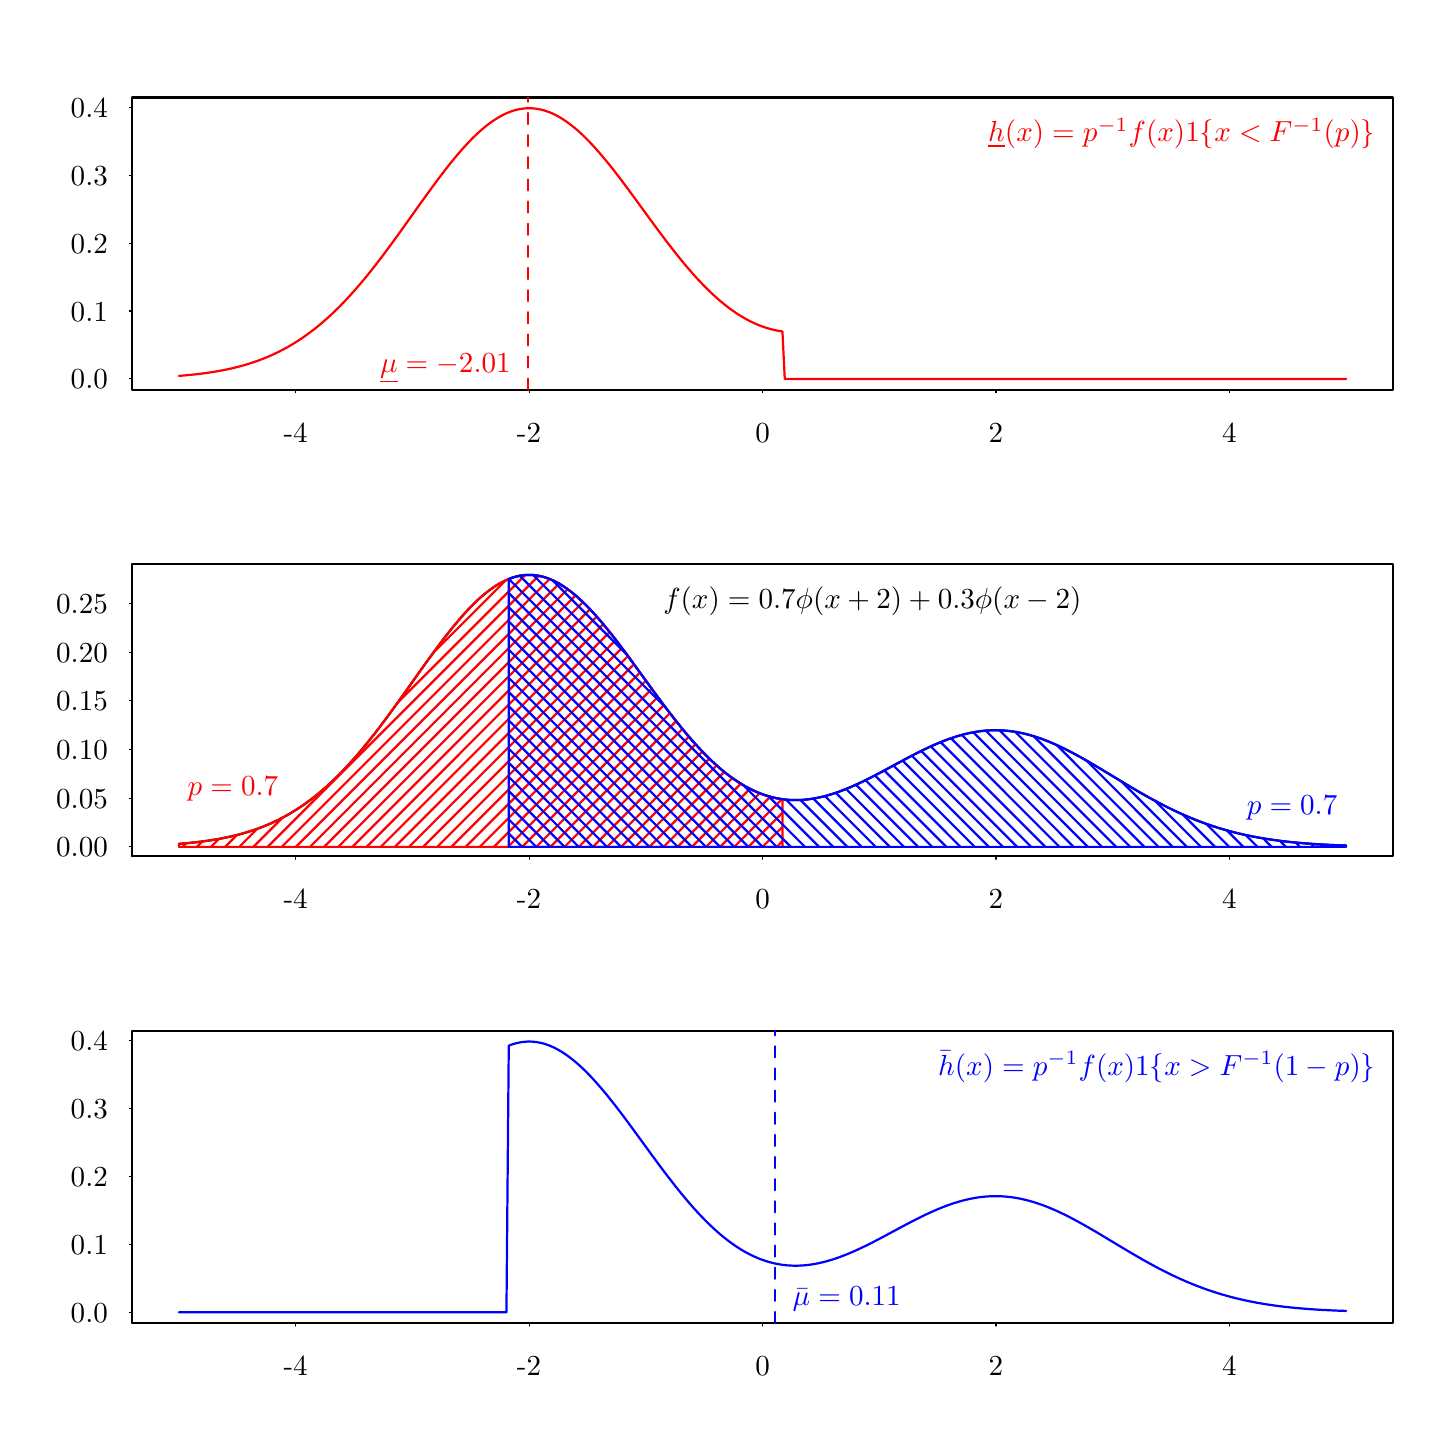
\begin{tikzpicture}[x=1pt,y=1pt]
\definecolor{fillColor}{RGB}{255,255,255}
\path[use as bounding box,fill=fillColor,fill opacity=0.00] (0,0) rectangle (505.89,505.89);
\begin{scope}
\path[clip] ( 37.80,375.06) rectangle (493.29,480.69);
\definecolor{drawColor}{RGB}{255,0,0}

\path[draw=drawColor,line width= 0.8pt,line join=round,line cap=round] ( 54.67,380.06) --
	( 55.52,380.13) --
	( 56.36,380.20) --
	( 57.21,380.27) --
	( 58.05,380.35) --
	( 58.90,380.43) --
	( 59.74,380.52) --
	( 60.59,380.61) --
	( 61.43,380.71) --
	( 62.28,380.81) --
	( 63.12,380.91) --
	( 63.97,381.03) --
	( 64.81,381.14) --
	( 65.66,381.27) --
	( 66.50,381.40) --
	( 67.35,381.53) --
	( 68.19,381.67) --
	( 69.04,381.82) --
	( 69.88,381.98) --
	( 70.73,382.14) --
	( 71.57,382.31) --
	( 72.42,382.49) --
	( 73.26,382.67) --
	( 74.11,382.87) --
	( 74.95,383.07) --
	( 75.80,383.28) --
	( 76.64,383.50) --
	( 77.49,383.73) --
	( 78.34,383.97) --
	( 79.18,384.22) --
	( 80.03,384.48) --
	( 80.87,384.75) --
	( 81.72,385.03) --
	( 82.56,385.32) --
	( 83.41,385.62) --
	( 84.25,385.94) --
	( 85.10,386.27) --
	( 85.94,386.60) --
	( 86.79,386.96) --
	( 87.63,387.32) --
	( 88.48,387.70) --
	( 89.32,388.09) --
	( 90.17,388.50) --
	( 91.01,388.91) --
	( 91.86,389.35) --
	( 92.70,389.79) --
	( 93.55,390.26) --
	( 94.39,390.73) --
	( 95.24,391.23) --
	( 96.08,391.74) --
	( 96.93,392.26) --
	( 97.77,392.80) --
	( 98.62,393.36) --
	( 99.47,393.93) --
	(100.31,394.52) --
	(101.16,395.12) --
	(102.00,395.75) --
	(102.85,396.39) --
	(103.69,397.04) --
	(104.54,397.72) --
	(105.38,398.41) --
	(106.23,399.12) --
	(107.07,399.84) --
	(107.92,400.59) --
	(108.76,401.35) --
	(109.61,402.13) --
	(110.45,402.93) --
	(111.30,403.74) --
	(112.14,404.57) --
	(112.99,405.42) --
	(113.83,406.28) --
	(114.68,407.17) --
	(115.52,408.07) --
	(116.37,408.98) --
	(117.21,409.92) --
	(118.06,410.86) --
	(118.90,411.83) --
	(119.75,412.81) --
	(120.59,413.80) --
	(121.44,414.82) --
	(122.29,415.84) --
	(123.13,416.88) --
	(123.98,417.93) --
	(124.82,419.00) --
	(125.67,420.08) --
	(126.51,421.17) --
	(127.36,422.27) --
	(128.20,423.38) --
	(129.05,424.50) --
	(129.89,425.64) --
	(130.74,426.78) --
	(131.58,427.93) --
	(132.43,429.09) --
	(133.27,430.25) --
	(134.12,431.42) --
	(134.96,432.60) --
	(135.81,433.78) --
	(136.65,434.96) --
	(137.50,436.15) --
	(138.34,437.34) --
	(139.19,438.52) --
	(140.03,439.71) --
	(140.88,440.90) --
	(141.72,442.09) --
	(142.57,443.27) --
	(143.41,444.45) --
	(144.26,445.62) --
	(145.11,446.78) --
	(145.95,447.94) --
	(146.80,449.09) --
	(147.64,450.24) --
	(148.49,451.37) --
	(149.33,452.49) --
	(150.18,453.59) --
	(151.02,454.68) --
	(151.87,455.76) --
	(152.71,456.82) --
	(153.56,457.87) --
	(154.40,458.90) --
	(155.25,459.90) --
	(156.09,460.89) --
	(156.94,461.86) --
	(157.78,462.80) --
	(158.63,463.72) --
	(159.47,464.62) --
	(160.32,465.49) --
	(161.16,466.34) --
	(162.01,467.15) --
	(162.85,467.94) --
	(163.70,468.71) --
	(164.54,469.44) --
	(165.39,470.14) --
	(166.24,470.81) --
	(167.08,471.44) --
	(167.93,472.05) --
	(168.77,472.62) --
	(169.62,473.15) --
	(170.46,473.65) --
	(171.31,474.12) --
	(172.15,474.55) --
	(173.00,474.94) --
	(173.84,475.30) --
	(174.69,475.62) --
	(175.53,475.90) --
	(176.38,476.14) --
	(177.22,476.34) --
	(178.07,476.51) --
	(178.91,476.63) --
	(179.76,476.72) --
	(180.60,476.77) --
	(181.45,476.78) --
	(182.29,476.75) --
	(183.14,476.68) --
	(183.98,476.57) --
	(184.83,476.42) --
	(185.67,476.24) --
	(186.52,476.01) --
	(187.36,475.75) --
	(188.21,475.45) --
	(189.06,475.11) --
	(189.90,474.74) --
	(190.75,474.32) --
	(191.59,473.88) --
	(192.44,473.39) --
	(193.28,472.87) --
	(194.13,472.32) --
	(194.97,471.73) --
	(195.82,471.11) --
	(196.66,470.46) --
	(197.51,469.78) --
	(198.35,469.06) --
	(199.20,468.32) --
	(200.04,467.55) --
	(200.89,466.75) --
	(201.73,465.92) --
	(202.58,465.06) --
	(203.42,464.18) --
	(204.27,463.28) --
	(205.11,462.35) --
	(205.96,461.40) --
	(206.80,460.43) --
	(207.65,459.44) --
	(208.49,458.43) --
	(209.34,457.41) --
	(210.19,456.36) --
	(211.03,455.30) --
	(211.88,454.23) --
	(212.72,453.14) --
	(213.57,452.04) --
	(214.41,450.93) --
	(215.26,449.81) --
	(216.10,448.68) --
	(216.95,447.54) --
	(217.79,446.40) --
	(218.64,445.24) --
	(219.48,444.09) --
	(220.33,442.93) --
	(221.17,441.77) --
	(222.02,440.61) --
	(222.86,439.45) --
	(223.71,438.29) --
	(224.55,437.13) --
	(225.40,435.97) --
	(226.24,434.82) --
	(227.09,433.67) --
	(227.93,432.53) --
	(228.78,431.40) --
	(229.62,430.27) --
	(230.47,429.15) --
	(231.31,428.04) --
	(232.16,426.94) --
	(233.01,425.86) --
	(233.85,424.78) --
	(234.70,423.72) --
	(235.54,422.67) --
	(236.39,421.63) --
	(237.23,420.61) --
	(238.08,419.60) --
	(238.92,418.61) --
	(239.77,417.64) --
	(240.61,416.68) --
	(241.46,415.74) --
	(242.30,414.82) --
	(243.15,413.92) --
	(243.99,413.04) --
	(244.84,412.18) --
	(245.68,411.33) --
	(246.53,410.51) --
	(247.37,409.71) --
	(248.22,408.93) --
	(249.06,408.17) --
	(249.91,407.43) --
	(250.75,406.71) --
	(251.60,406.02) --
	(252.44,405.35) --
	(253.29,404.70) --
	(254.13,404.07) --
	(254.98,403.47) --
	(255.83,402.89) --
	(256.67,402.33) --
	(257.52,401.80) --
	(258.36,401.29) --
	(259.21,400.80) --
	(260.05,400.33) --
	(260.90,399.89) --
	(261.74,399.48) --
	(262.59,399.08) --
	(263.43,398.71) --
	(264.28,398.36) --
	(265.12,398.03) --
	(265.97,397.73) --
	(266.81,397.45) --
	(267.66,397.19) --
	(268.50,396.96) --
	(269.35,396.74) --
	(270.19,396.55) --
	(271.04,396.38) --
	(271.88,396.24) --
	(272.73,396.11) --
	(273.57,378.97) --
	(274.42,378.97) --
	(275.26,378.97) --
	(276.11,378.97) --
	(276.96,378.97) --
	(277.80,378.97) --
	(278.65,378.97) --
	(279.49,378.97) --
	(280.34,378.97) --
	(281.18,378.97) --
	(282.03,378.97) --
	(282.87,378.97) --
	(283.72,378.97) --
	(284.56,378.97) --
	(285.41,378.97) --
	(286.25,378.97) --
	(287.10,378.97) --
	(287.94,378.97) --
	(288.79,378.97) --
	(289.63,378.97) --
	(290.48,378.97) --
	(291.32,378.97) --
	(292.17,378.97) --
	(293.01,378.97) --
	(293.86,378.97) --
	(294.70,378.97) --
	(295.55,378.97) --
	(296.39,378.97) --
	(297.24,378.97) --
	(298.08,378.97) --
	(298.93,378.97) --
	(299.78,378.97) --
	(300.62,378.97) --
	(301.47,378.97) --
	(302.31,378.97) --
	(303.16,378.97) --
	(304.00,378.97) --
	(304.85,378.97) --
	(305.69,378.97) --
	(306.54,378.97) --
	(307.38,378.97) --
	(308.23,378.97) --
	(309.07,378.97) --
	(309.92,378.97) --
	(310.76,378.97) --
	(311.61,378.97) --
	(312.45,378.97) --
	(313.30,378.97) --
	(314.14,378.97) --
	(314.99,378.97) --
	(315.83,378.97) --
	(316.68,378.97) --
	(317.52,378.97) --
	(318.37,378.97) --
	(319.21,378.97) --
	(320.06,378.97) --
	(320.90,378.97) --
	(321.75,378.97) --
	(322.60,378.97) --
	(323.44,378.97) --
	(324.29,378.97) --
	(325.13,378.97) --
	(325.98,378.97) --
	(326.82,378.97) --
	(327.67,378.97) --
	(328.51,378.97) --
	(329.36,378.97) --
	(330.20,378.97) --
	(331.05,378.97) --
	(331.89,378.97) --
	(332.74,378.97) --
	(333.58,378.97) --
	(334.43,378.97) --
	(335.27,378.97) --
	(336.12,378.97) --
	(336.96,378.97) --
	(337.81,378.97) --
	(338.65,378.97) --
	(339.50,378.97) --
	(340.34,378.97) --
	(341.19,378.97) --
	(342.03,378.97) --
	(342.88,378.97) --
	(343.73,378.97) --
	(344.57,378.97) --
	(345.42,378.97) --
	(346.26,378.97) --
	(347.11,378.97) --
	(347.95,378.97) --
	(348.80,378.97) --
	(349.64,378.97) --
	(350.49,378.97) --
	(351.33,378.97) --
	(352.18,378.97) --
	(353.02,378.97) --
	(353.87,378.97) --
	(354.71,378.97) --
	(355.56,378.97) --
	(356.40,378.97) --
	(357.25,378.97) --
	(358.09,378.97) --
	(358.94,378.97) --
	(359.78,378.97) --
	(360.63,378.97) --
	(361.47,378.97) --
	(362.32,378.97) --
	(363.16,378.97) --
	(364.01,378.97) --
	(364.85,378.97) --
	(365.70,378.97) --
	(366.55,378.97) --
	(367.39,378.97) --
	(368.24,378.97) --
	(369.08,378.97) --
	(369.93,378.97) --
	(370.77,378.97) --
	(371.62,378.97) --
	(372.46,378.97) --
	(373.31,378.97) --
	(374.15,378.97) --
	(375.00,378.97) --
	(375.84,378.97) --
	(376.69,378.97) --
	(377.53,378.97) --
	(378.38,378.97) --
	(379.22,378.97) --
	(380.07,378.97) --
	(380.91,378.97) --
	(381.76,378.97) --
	(382.60,378.97) --
	(383.45,378.97) --
	(384.29,378.97) --
	(385.14,378.97) --
	(385.98,378.97) --
	(386.83,378.97) --
	(387.68,378.97) --
	(388.52,378.97) --
	(389.37,378.97) --
	(390.21,378.97) --
	(391.06,378.97) --
	(391.90,378.97) --
	(392.75,378.97) --
	(393.59,378.97) --
	(394.44,378.97) --
	(395.28,378.97) --
	(396.13,378.97) --
	(396.97,378.97) --
	(397.82,378.97) --
	(398.66,378.97) --
	(399.51,378.97) --
	(400.35,378.97) --
	(401.20,378.97) --
	(402.04,378.97) --
	(402.89,378.97) --
	(403.73,378.97) --
	(404.58,378.97) --
	(405.42,378.97) --
	(406.27,378.97) --
	(407.11,378.97) --
	(407.96,378.97) --
	(408.80,378.97) --
	(409.65,378.97) --
	(410.50,378.97) --
	(411.34,378.97) --
	(412.19,378.97) --
	(413.03,378.97) --
	(413.88,378.97) --
	(414.72,378.97) --
	(415.57,378.97) --
	(416.41,378.97) --
	(417.26,378.97) --
	(418.10,378.97) --
	(418.95,378.97) --
	(419.79,378.97) --
	(420.64,378.97) --
	(421.48,378.97) --
	(422.33,378.97) --
	(423.17,378.97) --
	(424.02,378.97) --
	(424.86,378.97) --
	(425.71,378.97) --
	(426.55,378.97) --
	(427.40,378.97) --
	(428.24,378.97) --
	(429.09,378.97) --
	(429.93,378.97) --
	(430.78,378.97) --
	(431.62,378.97) --
	(432.47,378.97) --
	(433.32,378.97) --
	(434.16,378.97) --
	(435.01,378.97) --
	(435.85,378.97) --
	(436.70,378.97) --
	(437.54,378.97) --
	(438.39,378.97) --
	(439.23,378.97) --
	(440.08,378.97) --
	(440.92,378.97) --
	(441.77,378.97) --
	(442.61,378.97) --
	(443.46,378.97) --
	(444.30,378.97) --
	(445.15,378.97) --
	(445.99,378.97) --
	(446.84,378.97) --
	(447.68,378.97) --
	(448.53,378.97) --
	(449.37,378.97) --
	(450.22,378.97) --
	(451.06,378.97) --
	(451.91,378.97) --
	(452.75,378.97) --
	(453.60,378.97) --
	(454.45,378.97) --
	(455.29,378.97) --
	(456.14,378.97) --
	(456.98,378.97) --
	(457.83,378.97) --
	(458.67,378.97) --
	(459.52,378.97) --
	(460.36,378.97) --
	(461.21,378.97) --
	(462.05,378.97) --
	(462.90,378.97) --
	(463.74,378.97) --
	(464.59,378.97) --
	(465.43,378.97) --
	(466.28,378.97) --
	(467.12,378.97) --
	(467.97,378.97) --
	(468.81,378.97) --
	(469.66,378.97) --
	(470.50,378.97) --
	(471.35,378.97) --
	(472.19,378.97) --
	(473.04,378.97) --
	(473.88,378.97) --
	(474.73,378.97) --
	(475.57,378.97) --
	(476.42,378.97);
\end{scope}
\begin{scope}
\path[clip] (  0.00,  0.00) rectangle (505.89,505.89);
\definecolor{drawColor}{RGB}{0,0,0}

\path[draw=drawColor,line width= 0.4pt,line join=round,line cap=round] ( 96.84,375.06) -- (434.25,375.06);

\path[draw=drawColor,line width= 0.4pt,line join=round,line cap=round] ( 96.84,375.06) -- ( 96.84,374.00);

\path[draw=drawColor,line width= 0.4pt,line join=round,line cap=round] (181.19,375.06) -- (181.19,374.00);

\path[draw=drawColor,line width= 0.4pt,line join=round,line cap=round] (265.54,375.06) -- (265.54,374.00);

\path[draw=drawColor,line width= 0.4pt,line join=round,line cap=round] (349.89,375.06) -- (349.89,374.00);

\path[draw=drawColor,line width= 0.4pt,line join=round,line cap=round] (434.25,375.06) -- (434.25,374.00);

\node[text=drawColor,anchor=base,inner sep=0pt, outer sep=0pt, scale=  1.05] at ( 96.84,356.16) {-4};

\node[text=drawColor,anchor=base,inner sep=0pt, outer sep=0pt, scale=  1.05] at (181.19,356.16) {-2};

\node[text=drawColor,anchor=base,inner sep=0pt, outer sep=0pt, scale=  1.05] at (265.54,356.16) {0};

\node[text=drawColor,anchor=base,inner sep=0pt, outer sep=0pt, scale=  1.05] at (349.89,356.16) {2};

\node[text=drawColor,anchor=base,inner sep=0pt, outer sep=0pt, scale=  1.05] at (434.25,356.16) {4};

\path[draw=drawColor,line width= 0.4pt,line join=round,line cap=round] ( 37.80,378.97) -- ( 37.80,477.02);

\path[draw=drawColor,line width= 0.4pt,line join=round,line cap=round] ( 37.80,378.97) -- ( 36.74,378.97);

\path[draw=drawColor,line width= 0.4pt,line join=round,line cap=round] ( 37.80,403.49) -- ( 36.74,403.49);

\path[draw=drawColor,line width= 0.4pt,line join=round,line cap=round] ( 37.80,428.00) -- ( 36.74,428.00);

\path[draw=drawColor,line width= 0.4pt,line join=round,line cap=round] ( 37.80,452.51) -- ( 36.74,452.51);

\path[draw=drawColor,line width= 0.4pt,line join=round,line cap=round] ( 37.80,477.02) -- ( 36.74,477.02);

\node[text=drawColor,anchor=base east,inner sep=0pt, outer sep=0pt, scale=  1.05] at ( 28.98,375.36) {0.0};

\node[text=drawColor,anchor=base east,inner sep=0pt, outer sep=0pt, scale=  1.05] at ( 28.98,399.87) {0.1};

\node[text=drawColor,anchor=base east,inner sep=0pt, outer sep=0pt, scale=  1.05] at ( 28.98,424.38) {0.2};

\node[text=drawColor,anchor=base east,inner sep=0pt, outer sep=0pt, scale=  1.05] at ( 28.98,448.90) {0.3};

\node[text=drawColor,anchor=base east,inner sep=0pt, outer sep=0pt, scale=  1.05] at ( 28.98,473.41) {0.4};

\path[draw=drawColor,line width= 0.8pt,line join=round,line cap=round] ( 37.80,375.06) --
	(493.29,375.06) --
	(493.29,480.69) --
	( 37.80,480.69) --
	( 37.80,375.06);
\end{scope}
\begin{scope}
\path[clip] ( 37.80,375.06) rectangle (493.29,480.69);
\definecolor{drawColor}{RGB}{255,0,0}

\node[text=drawColor,anchor=base east,inner sep=0pt, outer sep=0pt, scale=  1.05] at (486.99,464.59) {$\underline{h}(x) = p^{-1}f(x) 1\{x < F^{-1}(p)\}$};

\path[draw=drawColor,line width= 0.8pt,dash pattern=on 4pt off 4pt ,line join=round,line cap=round] (180.82,375.06) -- (180.82,480.69);

\node[text=drawColor,anchor=base east,inner sep=0pt, outer sep=0pt, scale=  1.05] at (174.52,381.45) {$\underline{\mu} = -2.01$};
\end{scope}
\begin{scope}
\path[clip] ( 37.80,206.43) rectangle (493.29,312.06);
\definecolor{drawColor}{RGB}{0,0,0}

\path[draw=drawColor,line width= 0.8pt,line join=round,line cap=round] ( 54.67,210.97) --
	( 55.52,211.03) --
	( 56.36,211.10) --
	( 57.21,211.18) --
	( 58.05,211.26) --
	( 58.90,211.34) --
	( 59.74,211.43) --
	( 60.59,211.52) --
	( 61.43,211.62) --
	( 62.28,211.72) --
	( 63.12,211.83) --
	( 63.97,211.94) --
	( 64.81,212.06) --
	( 65.66,212.18) --
	( 66.50,212.31) --
	( 67.35,212.45) --
	( 68.19,212.59) --
	( 69.04,212.74) --
	( 69.88,212.89) --
	( 70.73,213.06) --
	( 71.57,213.23) --
	( 72.42,213.41) --
	( 73.26,213.59) --
	( 74.11,213.79) --
	( 74.95,213.99) --
	( 75.80,214.20) --
	( 76.64,214.42) --
	( 77.49,214.65) --
	( 78.34,214.90) --
	( 79.18,215.15) --
	( 80.03,215.41) --
	( 80.87,215.68) --
	( 81.72,215.96) --
	( 82.56,216.25) --
	( 83.41,216.56) --
	( 84.25,216.87) --
	( 85.10,217.20) --
	( 85.94,217.54) --
	( 86.79,217.90) --
	( 87.63,218.26) --
	( 88.48,218.64) --
	( 89.32,219.04) --
	( 90.17,219.44) --
	( 91.01,219.86) --
	( 91.86,220.30) --
	( 92.70,220.75) --
	( 93.55,221.21) --
	( 94.39,221.69) --
	( 95.24,222.19) --
	( 96.08,222.70) --
	( 96.93,223.23) --
	( 97.77,223.77) --
	( 98.62,224.33) --
	( 99.47,224.90) --
	(100.31,225.49) --
	(101.16,226.10) --
	(102.00,226.73) --
	(102.85,227.37) --
	(103.69,228.03) --
	(104.54,228.71) --
	(105.38,229.40) --
	(106.23,230.12) --
	(107.07,230.85) --
	(107.92,231.59) --
	(108.76,232.36) --
	(109.61,233.14) --
	(110.45,233.94) --
	(111.30,234.76) --
	(112.14,235.59) --
	(112.99,236.45) --
	(113.83,237.32) --
	(114.68,238.20) --
	(115.52,239.11) --
	(116.37,240.03) --
	(117.21,240.97) --
	(118.06,241.92) --
	(118.90,242.89) --
	(119.75,243.87) --
	(120.59,244.87) --
	(121.44,245.89) --
	(122.29,246.92) --
	(123.13,247.96) --
	(123.98,249.02) --
	(124.82,250.09) --
	(125.67,251.17) --
	(126.51,252.27) --
	(127.36,253.38) --
	(128.20,254.50) --
	(129.05,255.62) --
	(129.89,256.76) --
	(130.74,257.91) --
	(131.58,259.07) --
	(132.43,260.23) --
	(133.27,261.40) --
	(134.12,262.58) --
	(134.96,263.76) --
	(135.81,264.94) --
	(136.65,266.13) --
	(137.50,267.32) --
	(138.34,268.52) --
	(139.19,269.71) --
	(140.03,270.91) --
	(140.88,272.10) --
	(141.72,273.29) --
	(142.57,274.48) --
	(143.41,275.66) --
	(144.26,276.84) --
	(145.11,278.01) --
	(145.95,279.18) --
	(146.80,280.33) --
	(147.64,281.48) --
	(148.49,282.61) --
	(149.33,283.74) --
	(150.18,284.85) --
	(151.02,285.95) --
	(151.87,287.03) --
	(152.71,288.10) --
	(153.56,289.15) --
	(154.40,290.18) --
	(155.25,291.19) --
	(156.09,292.19) --
	(156.94,293.16) --
	(157.78,294.11) --
	(158.63,295.03) --
	(159.47,295.93) --
	(160.32,296.81) --
	(161.16,297.66) --
	(162.01,298.48) --
	(162.85,299.27) --
	(163.70,300.04) --
	(164.54,300.77) --
	(165.39,301.47) --
	(166.24,302.15) --
	(167.08,302.79) --
	(167.93,303.39) --
	(168.77,303.97) --
	(169.62,304.51) --
	(170.46,305.01) --
	(171.31,305.48) --
	(172.15,305.91) --
	(173.00,306.30) --
	(173.84,306.66) --
	(174.69,306.98) --
	(175.53,307.26) --
	(176.38,307.50) --
	(177.22,307.71) --
	(178.07,307.88) --
	(178.91,308.00) --
	(179.76,308.09) --
	(180.60,308.14) --
	(181.45,308.15) --
	(182.29,308.12) --
	(183.14,308.05) --
	(183.98,307.94) --
	(184.83,307.79) --
	(185.67,307.60) --
	(186.52,307.38) --
	(187.36,307.11) --
	(188.21,306.81) --
	(189.06,306.47) --
	(189.90,306.10) --
	(190.75,305.68) --
	(191.59,305.23) --
	(192.44,304.75) --
	(193.28,304.22) --
	(194.13,303.67) --
	(194.97,303.08) --
	(195.82,302.46) --
	(196.66,301.80) --
	(197.51,301.12) --
	(198.35,300.40) --
	(199.20,299.65) --
	(200.04,298.87) --
	(200.89,298.07) --
	(201.73,297.24) --
	(202.58,296.38) --
	(203.42,295.49) --
	(204.27,294.59) --
	(205.11,293.65) --
	(205.96,292.70) --
	(206.80,291.73) --
	(207.65,290.73) --
	(208.49,289.72) --
	(209.34,288.68) --
	(210.19,287.63) --
	(211.03,286.57) --
	(211.88,285.49) --
	(212.72,284.40) --
	(213.57,283.29) --
	(214.41,282.18) --
	(215.26,281.05) --
	(216.10,279.91) --
	(216.95,278.77) --
	(217.79,277.62) --
	(218.64,276.46) --
	(219.48,275.30) --
	(220.33,274.14) --
	(221.17,272.97) --
	(222.02,271.81) --
	(222.86,270.64) --
	(223.71,269.47) --
	(224.55,268.31) --
	(225.40,267.15) --
	(226.24,265.99) --
	(227.09,264.84) --
	(227.93,263.69) --
	(228.78,262.55) --
	(229.62,261.42) --
	(230.47,260.29) --
	(231.31,259.18) --
	(232.16,258.08) --
	(233.01,256.98) --
	(233.85,255.90) --
	(234.70,254.83) --
	(235.54,253.78) --
	(236.39,252.74) --
	(237.23,251.71) --
	(238.08,250.70) --
	(238.92,249.71) --
	(239.77,248.73) --
	(240.61,247.77) --
	(241.46,246.82) --
	(242.30,245.90) --
	(243.15,244.99) --
	(243.99,244.10) --
	(244.84,243.24) --
	(245.68,242.39) --
	(246.53,241.56) --
	(247.37,240.76) --
	(248.22,239.97) --
	(249.06,239.21) --
	(249.91,238.47) --
	(250.75,237.75) --
	(251.60,237.05) --
	(252.44,236.38) --
	(253.29,235.73) --
	(254.13,235.10) --
	(254.98,234.49) --
	(255.83,233.91) --
	(256.67,233.35) --
	(257.52,232.81) --
	(258.36,232.30) --
	(259.21,231.81) --
	(260.05,231.34) --
	(260.90,230.90) --
	(261.74,230.48) --
	(262.59,230.08) --
	(263.43,229.70) --
	(264.28,229.35) --
	(265.12,229.03) --
	(265.97,228.72) --
	(266.81,228.44) --
	(267.66,228.18) --
	(268.50,227.94) --
	(269.35,227.73) --
	(270.19,227.54) --
	(271.04,227.37) --
	(271.88,227.22) --
	(272.73,227.09) --
	(273.57,226.99) --
	(274.42,226.90) --
	(275.26,226.84) --
	(276.11,226.80) --
	(276.96,226.78) --
	(277.80,226.77) --
	(278.65,226.79) --
	(279.49,226.83) --
	(280.34,226.88) --
	(281.18,226.96) --
	(282.03,227.05) --
	(282.87,227.16) --
	(283.72,227.29) --
	(284.56,227.44) --
	(285.41,227.60) --
	(286.25,227.78) --
	(287.10,227.97) --
	(287.94,228.18) --
	(288.79,228.41) --
	(289.63,228.65) --
	(290.48,228.91) --
	(291.32,229.18) --
	(292.17,229.46) --
	(293.01,229.76) --
	(293.86,230.07) --
	(294.70,230.39) --
	(295.55,230.72) --
	(296.39,231.07) --
	(297.24,231.42) --
	(298.08,231.79) --
	(298.93,232.16) --
	(299.78,232.55) --
	(300.62,232.94) --
	(301.47,233.34) --
	(302.31,233.75) --
	(303.16,234.16) --
	(304.00,234.59) --
	(304.85,235.01) --
	(305.69,235.45) --
	(306.54,235.89) --
	(307.38,236.33) --
	(308.23,236.78) --
	(309.07,237.23) --
	(309.92,237.68) --
	(310.76,238.13) --
	(311.61,238.59) --
	(312.45,239.05) --
	(313.30,239.50) --
	(314.14,239.96) --
	(314.99,240.41) --
	(315.83,240.87) --
	(316.68,241.32) --
	(317.52,241.77) --
	(318.37,242.22) --
	(319.21,242.66) --
	(320.06,243.10) --
	(320.90,243.53) --
	(321.75,243.96) --
	(322.60,244.38) --
	(323.44,244.80) --
	(324.29,245.21) --
	(325.13,245.61) --
	(325.98,246.00) --
	(326.82,246.39) --
	(327.67,246.76) --
	(328.51,247.13) --
	(329.36,247.48) --
	(330.20,247.83) --
	(331.05,248.16) --
	(331.89,248.49) --
	(332.74,248.80) --
	(333.58,249.09) --
	(334.43,249.38) --
	(335.27,249.65) --
	(336.12,249.91) --
	(336.96,250.16) --
	(337.81,250.39) --
	(338.65,250.61) --
	(339.50,250.81) --
	(340.34,251.00) --
	(341.19,251.17) --
	(342.03,251.33) --
	(342.88,251.47) --
	(343.73,251.60) --
	(344.57,251.71) --
	(345.42,251.80) --
	(346.26,251.88) --
	(347.11,251.94) --
	(347.95,251.98) --
	(348.80,252.01) --
	(349.64,252.02) --
	(350.49,252.01) --
	(351.33,251.99) --
	(352.18,251.95) --
	(353.02,251.89) --
	(353.87,251.82) --
	(354.71,251.73) --
	(355.56,251.63) --
	(356.40,251.51) --
	(357.25,251.37) --
	(358.09,251.21) --
	(358.94,251.04) --
	(359.78,250.86) --
	(360.63,250.66) --
	(361.47,250.44) --
	(362.32,250.21) --
	(363.16,249.96) --
	(364.01,249.70) --
	(364.85,249.43) --
	(365.70,249.14) --
	(366.55,248.84) --
	(367.39,248.52) --
	(368.24,248.19) --
	(369.08,247.85) --
	(369.93,247.50) --
	(370.77,247.13) --
	(371.62,246.76) --
	(372.46,246.37) --
	(373.31,245.98) --
	(374.15,245.57) --
	(375.00,245.15) --
	(375.84,244.73) --
	(376.69,244.29) --
	(377.53,243.85) --
	(378.38,243.40) --
	(379.22,242.94) --
	(380.07,242.48) --
	(380.91,242.01) --
	(381.76,241.53) --
	(382.60,241.05) --
	(383.45,240.56) --
	(384.29,240.07) --
	(385.14,239.58) --
	(385.98,239.08) --
	(386.83,238.57) --
	(387.68,238.07) --
	(388.52,237.56) --
	(389.37,237.05) --
	(390.21,236.54) --
	(391.06,236.03) --
	(391.90,235.52) --
	(392.75,235.01) --
	(393.59,234.50) --
	(394.44,233.98) --
	(395.28,233.48) --
	(396.13,232.97) --
	(396.97,232.46) --
	(397.82,231.96) --
	(398.66,231.46) --
	(399.51,230.96) --
	(400.35,230.46) --
	(401.20,229.97) --
	(402.04,229.48) --
	(402.89,229.00) --
	(403.73,228.52) --
	(404.58,228.04) --
	(405.42,227.57) --
	(406.27,227.11) --
	(407.11,226.65) --
	(407.96,226.20) --
	(408.80,225.75) --
	(409.65,225.31) --
	(410.50,224.87) --
	(411.34,224.45) --
	(412.19,224.02) --
	(413.03,223.61) --
	(413.88,223.20) --
	(414.72,222.80) --
	(415.57,222.40) --
	(416.41,222.02) --
	(417.26,221.64) --
	(418.10,221.26) --
	(418.95,220.90) --
	(419.79,220.54) --
	(420.64,220.19) --
	(421.48,219.85) --
	(422.33,219.51) --
	(423.17,219.18) --
	(424.02,218.86) --
	(424.86,218.55) --
	(425.71,218.24) --
	(426.55,217.95) --
	(427.40,217.66) --
	(428.24,217.37) --
	(429.09,217.10) --
	(429.93,216.83) --
	(430.78,216.57) --
	(431.62,216.32) --
	(432.47,216.07) --
	(433.32,215.83) --
	(434.16,215.60) --
	(435.01,215.37) --
	(435.85,215.15) --
	(436.70,214.94) --
	(437.54,214.73) --
	(438.39,214.53) --
	(439.23,214.34) --
	(440.08,214.16) --
	(440.92,213.98) --
	(441.77,213.80) --
	(442.61,213.63) --
	(443.46,213.47) --
	(444.30,213.31) --
	(445.15,213.16) --
	(445.99,213.02) --
	(446.84,212.87) --
	(447.68,212.74) --
	(448.53,212.61) --
	(449.37,212.48) --
	(450.22,212.36) --
	(451.06,212.25) --
	(451.91,212.13) --
	(452.75,212.03) --
	(453.60,211.92) --
	(454.45,211.82) --
	(455.29,211.73) --
	(456.14,211.64) --
	(456.98,211.55) --
	(457.83,211.47) --
	(458.67,211.39) --
	(459.52,211.31) --
	(460.36,211.24) --
	(461.21,211.17) --
	(462.05,211.10) --
	(462.90,211.04) --
	(463.74,210.98) --
	(464.59,210.92) --
	(465.43,210.86) --
	(466.28,210.81) --
	(467.12,210.76) --
	(467.97,210.71) --
	(468.81,210.67) --
	(469.66,210.62) --
	(470.50,210.58) --
	(471.35,210.54) --
	(472.19,210.50) --
	(473.04,210.47) --
	(473.88,210.43) --
	(474.73,210.40) --
	(475.57,210.37) --
	(476.42,210.34);
\end{scope}
\begin{scope}
\path[clip] (  0.00,  0.00) rectangle (505.89,505.89);
\definecolor{drawColor}{RGB}{0,0,0}

\path[draw=drawColor,line width= 0.4pt,line join=round,line cap=round] ( 96.84,206.43) -- (434.25,206.43);

\path[draw=drawColor,line width= 0.4pt,line join=round,line cap=round] ( 96.84,206.43) -- ( 96.84,205.37);

\path[draw=drawColor,line width= 0.4pt,line join=round,line cap=round] (181.19,206.43) -- (181.19,205.37);

\path[draw=drawColor,line width= 0.4pt,line join=round,line cap=round] (265.54,206.43) -- (265.54,205.37);

\path[draw=drawColor,line width= 0.4pt,line join=round,line cap=round] (349.89,206.43) -- (349.89,205.37);

\path[draw=drawColor,line width= 0.4pt,line join=round,line cap=round] (434.25,206.43) -- (434.25,205.37);

\node[text=drawColor,anchor=base,inner sep=0pt, outer sep=0pt, scale=  1.05] at ( 96.84,187.53) {-4};

\node[text=drawColor,anchor=base,inner sep=0pt, outer sep=0pt, scale=  1.05] at (181.19,187.53) {-2};

\node[text=drawColor,anchor=base,inner sep=0pt, outer sep=0pt, scale=  1.05] at (265.54,187.53) {0};

\node[text=drawColor,anchor=base,inner sep=0pt, outer sep=0pt, scale=  1.05] at (349.89,187.53) {2};

\node[text=drawColor,anchor=base,inner sep=0pt, outer sep=0pt, scale=  1.05] at (434.25,187.53) {4};

\path[draw=drawColor,line width= 0.4pt,line join=round,line cap=round] ( 37.80,209.87) -- ( 37.80,297.84);

\path[draw=drawColor,line width= 0.4pt,line join=round,line cap=round] ( 37.80,209.87) -- ( 36.74,209.87);

\path[draw=drawColor,line width= 0.4pt,line join=round,line cap=round] ( 37.80,227.47) -- ( 36.74,227.47);

\path[draw=drawColor,line width= 0.4pt,line join=round,line cap=round] ( 37.80,245.06) -- ( 36.74,245.06);

\path[draw=drawColor,line width= 0.4pt,line join=round,line cap=round] ( 37.80,262.65) -- ( 36.74,262.65);

\path[draw=drawColor,line width= 0.4pt,line join=round,line cap=round] ( 37.80,280.25) -- ( 36.74,280.25);

\path[draw=drawColor,line width= 0.4pt,line join=round,line cap=round] ( 37.80,297.84) -- ( 36.74,297.84);

\node[text=drawColor,anchor=base east,inner sep=0pt, outer sep=0pt, scale=  1.05] at ( 28.98,206.26) {0.00};

\node[text=drawColor,anchor=base east,inner sep=0pt, outer sep=0pt, scale=  1.05] at ( 28.98,223.85) {0.05};

\node[text=drawColor,anchor=base east,inner sep=0pt, outer sep=0pt, scale=  1.05] at ( 28.98,241.44) {0.10};

\node[text=drawColor,anchor=base east,inner sep=0pt, outer sep=0pt, scale=  1.05] at ( 28.98,259.04) {0.15};

\node[text=drawColor,anchor=base east,inner sep=0pt, outer sep=0pt, scale=  1.05] at ( 28.98,276.63) {0.20};

\node[text=drawColor,anchor=base east,inner sep=0pt, outer sep=0pt, scale=  1.05] at ( 28.98,294.22) {0.25};

\path[draw=drawColor,line width= 0.8pt,line join=round,line cap=round] ( 37.80,206.43) --
	(493.29,206.43) --
	(493.29,312.06) --
	( 37.80,312.06) --
	( 37.80,206.43);
\end{scope}
\begin{scope}
\path[clip] ( 37.80,206.43) rectangle (493.29,312.06);
\definecolor{drawColor}{RGB}{255,0,0}

\path[draw=drawColor,line width= 0.8pt,line join=round,line cap=round] ( 56.02,209.87) -- ( 57.34,211.19);

\path[draw=drawColor,line width= 0.8pt,line join=round,line cap=round] ( 61.13,209.87) -- ( 63.08,211.82);

\path[draw=drawColor,line width= 0.8pt,line join=round,line cap=round] ( 66.24,209.87) -- ( 69.12,212.75);

\path[draw=drawColor,line width= 0.8pt,line join=round,line cap=round] ( 71.36,209.87) -- ( 75.64,214.16);

\path[draw=drawColor,line width= 0.8pt,line join=round,line cap=round] ( 76.47,209.87) -- ( 83.00,216.41);

\path[draw=drawColor,line width= 0.8pt,line join=round,line cap=round] (146.45,279.86) -- (172.80,306.21);

\path[draw=drawColor,line width= 0.8pt,line join=round,line cap=round] ( 81.58,209.87) -- ( 92.16,220.46);

\path[draw=drawColor,line width= 0.8pt,line join=round,line cap=round] (133.71,262.01) -- (179.79,308.09);

\path[draw=drawColor,line width= 0.8pt,line join=round,line cap=round] ( 86.69,209.87) -- (184.64,307.82);

\path[draw=drawColor,line width= 0.8pt,line join=round,line cap=round] ( 91.80,209.87) -- (188.58,306.66);

\path[draw=drawColor,line width= 0.8pt,line join=round,line cap=round] ( 96.91,209.87) -- (192.02,304.99);

\path[draw=drawColor,line width= 0.8pt,line join=round,line cap=round] (102.02,209.87) -- (195.12,302.97);

\path[draw=drawColor,line width= 0.8pt,line join=round,line cap=round] (107.13,209.87) -- (197.97,300.72);

\path[draw=drawColor,line width= 0.8pt,line join=round,line cap=round] (112.24,209.87) -- (200.65,298.29);

\path[draw=drawColor,line width= 0.8pt,line join=round,line cap=round] (117.35,209.87) -- (203.20,295.73);

\path[draw=drawColor,line width= 0.8pt,line join=round,line cap=round] (122.46,209.87) -- (205.64,293.06);

\path[draw=drawColor,line width= 0.8pt,line join=round,line cap=round] (127.57,209.87) -- (208.00,290.31);

\path[draw=drawColor,line width= 0.8pt,line join=round,line cap=round] (132.68,209.87) -- (210.30,287.49);

\path[draw=drawColor,line width= 0.8pt,line join=round,line cap=round] (137.79,209.87) -- (212.54,284.63);

\path[draw=drawColor,line width= 0.8pt,line join=round,line cap=round] (142.90,209.87) -- (214.75,281.72);

\path[draw=drawColor,line width= 0.8pt,line join=round,line cap=round] (148.01,209.87) -- (216.93,278.79);

\path[draw=drawColor,line width= 0.8pt,line join=round,line cap=round] (153.12,209.87) -- (219.09,275.84);

\path[draw=drawColor,line width= 0.8pt,line join=round,line cap=round] (158.23,209.87) -- (221.24,272.88);

\path[draw=drawColor,line width= 0.8pt,line join=round,line cap=round] (163.34,209.87) -- (223.39,269.92);

\path[draw=drawColor,line width= 0.8pt,line join=round,line cap=round] (168.45,209.87) -- (225.54,266.96);

\path[draw=drawColor,line width= 0.8pt,line join=round,line cap=round] (173.56,209.87) -- (227.70,264.01);

\path[draw=drawColor,line width= 0.8pt,line join=round,line cap=round] (178.67,209.87) -- (229.88,261.08);

\path[draw=drawColor,line width= 0.8pt,line join=round,line cap=round] (183.78,209.87) -- (232.08,258.18);

\path[draw=drawColor,line width= 0.8pt,line join=round,line cap=round] (188.89,209.87) -- (234.32,255.31);

\path[draw=drawColor,line width= 0.8pt,line join=round,line cap=round] (194.00,209.87) -- (236.60,252.47);

\path[draw=drawColor,line width= 0.8pt,line join=round,line cap=round] (199.11,209.87) -- (238.93,249.69);

\path[draw=drawColor,line width= 0.8pt,line join=round,line cap=round] (204.22,209.87) -- (241.32,246.97);

\path[draw=drawColor,line width= 0.8pt,line join=round,line cap=round] (209.33,209.87) -- (243.78,244.32);

\path[draw=drawColor,line width= 0.8pt,line join=round,line cap=round] (214.44,209.87) -- (246.33,241.76);

\path[draw=drawColor,line width= 0.8pt,line join=round,line cap=round] (219.55,209.87) -- (248.97,239.29);

\path[draw=drawColor,line width= 0.8pt,line join=round,line cap=round] (224.66,209.87) -- (251.73,236.95);

\path[draw=drawColor,line width= 0.8pt,line join=round,line cap=round] (229.77,209.87) -- (254.64,234.74);

\path[draw=drawColor,line width= 0.8pt,line join=round,line cap=round] (234.88,209.87) -- (257.70,232.70);

\path[draw=drawColor,line width= 0.8pt,line join=round,line cap=round] (239.99,209.87) -- (260.98,230.86);

\path[draw=drawColor,line width= 0.8pt,line join=round,line cap=round] (245.10,209.87) -- (264.50,229.27);

\path[draw=drawColor,line width= 0.8pt,line join=round,line cap=round] (250.21,209.87) -- (268.33,227.99);

\path[draw=drawColor,line width= 0.8pt,line join=round,line cap=round] (255.32,209.87) -- (272.57,227.12);

\path[draw=drawColor,line width= 0.8pt,line join=round,line cap=round] (260.43,209.87) -- (272.73,222.17);

\path[draw=drawColor,line width= 0.8pt,line join=round,line cap=round] (265.54,209.87) -- (272.73,217.06);

\path[draw=drawColor,line width= 0.8pt,line join=round,line cap=round] (270.66,209.87) -- (272.73,211.95);

\path[draw=drawColor,line width= 0.8pt,line join=round,line cap=round] ( 54.67,209.87) --
	( 55.52,209.87) --
	( 56.36,209.87) --
	( 57.21,209.87) --
	( 58.05,209.87) --
	( 58.90,209.87) --
	( 59.74,209.87) --
	( 60.59,209.87) --
	( 61.43,209.87) --
	( 62.28,209.87) --
	( 63.12,209.87) --
	( 63.97,209.87) --
	( 64.81,209.87) --
	( 65.66,209.87) --
	( 66.50,209.87) --
	( 67.35,209.87) --
	( 68.19,209.87) --
	( 69.04,209.87) --
	( 69.88,209.87) --
	( 70.73,209.87) --
	( 71.57,209.87) --
	( 72.42,209.87) --
	( 73.26,209.87) --
	( 74.11,209.87) --
	( 74.95,209.87) --
	( 75.80,209.87) --
	( 76.64,209.87) --
	( 77.49,209.87) --
	( 78.34,209.87) --
	( 79.18,209.87) --
	( 80.03,209.87) --
	( 80.87,209.87) --
	( 81.72,209.87) --
	( 82.56,209.87) --
	( 83.41,209.87) --
	( 84.25,209.87) --
	( 85.10,209.87) --
	( 85.94,209.87) --
	( 86.79,209.87) --
	( 87.63,209.87) --
	( 88.48,209.87) --
	( 89.32,209.87) --
	( 90.17,209.87) --
	( 91.01,209.87) --
	( 91.86,209.87) --
	( 92.70,209.87) --
	( 93.55,209.87) --
	( 94.39,209.87) --
	( 95.24,209.87) --
	( 96.08,209.87) --
	( 96.93,209.87) --
	( 97.77,209.87) --
	( 98.62,209.87) --
	( 99.47,209.87) --
	(100.31,209.87) --
	(101.16,209.87) --
	(102.00,209.87) --
	(102.85,209.87) --
	(103.69,209.87) --
	(104.54,209.87) --
	(105.38,209.87) --
	(106.23,209.87) --
	(107.07,209.87) --
	(107.92,209.87) --
	(108.76,209.87) --
	(109.61,209.87) --
	(110.45,209.87) --
	(111.30,209.87) --
	(112.14,209.87) --
	(112.99,209.87) --
	(113.83,209.87) --
	(114.68,209.87) --
	(115.52,209.87) --
	(116.37,209.87) --
	(117.21,209.87) --
	(118.06,209.87) --
	(118.90,209.87) --
	(119.75,209.87) --
	(120.59,209.87) --
	(121.44,209.87) --
	(122.29,209.87) --
	(123.13,209.87) --
	(123.98,209.87) --
	(124.82,209.87) --
	(125.67,209.87) --
	(126.51,209.87) --
	(127.36,209.87) --
	(128.20,209.87) --
	(129.05,209.87) --
	(129.89,209.87) --
	(130.74,209.87) --
	(131.58,209.87) --
	(132.43,209.87) --
	(133.27,209.87) --
	(134.12,209.87) --
	(134.96,209.87) --
	(135.81,209.87) --
	(136.65,209.87) --
	(137.50,209.87) --
	(138.34,209.87) --
	(139.19,209.87) --
	(140.03,209.87) --
	(140.88,209.87) --
	(141.72,209.87) --
	(142.57,209.87) --
	(143.41,209.87) --
	(144.26,209.87) --
	(145.11,209.87) --
	(145.95,209.87) --
	(146.80,209.87) --
	(147.64,209.87) --
	(148.49,209.87) --
	(149.33,209.87) --
	(150.18,209.87) --
	(151.02,209.87) --
	(151.87,209.87) --
	(152.71,209.87) --
	(153.56,209.87) --
	(154.40,209.87) --
	(155.25,209.87) --
	(156.09,209.87) --
	(156.94,209.87) --
	(157.78,209.87) --
	(158.63,209.87) --
	(159.47,209.87) --
	(160.32,209.87) --
	(161.16,209.87) --
	(162.01,209.87) --
	(162.85,209.87) --
	(163.70,209.87) --
	(164.54,209.87) --
	(165.39,209.87) --
	(166.24,209.87) --
	(167.08,209.87) --
	(167.93,209.87) --
	(168.77,209.87) --
	(169.62,209.87) --
	(170.46,209.87) --
	(171.31,209.87) --
	(172.15,209.87) --
	(173.00,209.87) --
	(173.84,209.87) --
	(174.69,209.87) --
	(175.53,209.87) --
	(176.38,209.87) --
	(177.22,209.87) --
	(178.07,209.87) --
	(178.91,209.87) --
	(179.76,209.87) --
	(180.60,209.87) --
	(181.45,209.87) --
	(182.29,209.87) --
	(183.14,209.87) --
	(183.98,209.87) --
	(184.83,209.87) --
	(185.67,209.87) --
	(186.52,209.87) --
	(187.36,209.87) --
	(188.21,209.87) --
	(189.06,209.87) --
	(189.90,209.87) --
	(190.75,209.87) --
	(191.59,209.87) --
	(192.44,209.87) --
	(193.28,209.87) --
	(194.13,209.87) --
	(194.97,209.87) --
	(195.82,209.87) --
	(196.66,209.87) --
	(197.51,209.87) --
	(198.35,209.87) --
	(199.20,209.87) --
	(200.04,209.87) --
	(200.89,209.87) --
	(201.73,209.87) --
	(202.58,209.87) --
	(203.42,209.87) --
	(204.27,209.87) --
	(205.11,209.87) --
	(205.96,209.87) --
	(206.80,209.87) --
	(207.65,209.87) --
	(208.49,209.87) --
	(209.34,209.87) --
	(210.19,209.87) --
	(211.03,209.87) --
	(211.88,209.87) --
	(212.72,209.87) --
	(213.57,209.87) --
	(214.41,209.87) --
	(215.26,209.87) --
	(216.10,209.87) --
	(216.95,209.87) --
	(217.79,209.87) --
	(218.64,209.87) --
	(219.48,209.87) --
	(220.33,209.87) --
	(221.17,209.87) --
	(222.02,209.87) --
	(222.86,209.87) --
	(223.71,209.87) --
	(224.55,209.87) --
	(225.40,209.87) --
	(226.24,209.87) --
	(227.09,209.87) --
	(227.93,209.87) --
	(228.78,209.87) --
	(229.62,209.87) --
	(230.47,209.87) --
	(231.31,209.87) --
	(232.16,209.87) --
	(233.01,209.87) --
	(233.85,209.87) --
	(234.70,209.87) --
	(235.54,209.87) --
	(236.39,209.87) --
	(237.23,209.87) --
	(238.08,209.87) --
	(238.92,209.87) --
	(239.77,209.87) --
	(240.61,209.87) --
	(241.46,209.87) --
	(242.30,209.87) --
	(243.15,209.87) --
	(243.99,209.87) --
	(244.84,209.87) --
	(245.68,209.87) --
	(246.53,209.87) --
	(247.37,209.87) --
	(248.22,209.87) --
	(249.06,209.87) --
	(249.91,209.87) --
	(250.75,209.87) --
	(251.60,209.87) --
	(252.44,209.87) --
	(253.29,209.87) --
	(254.13,209.87) --
	(254.98,209.87) --
	(255.83,209.87) --
	(256.67,209.87) --
	(257.52,209.87) --
	(258.36,209.87) --
	(259.21,209.87) --
	(260.05,209.87) --
	(260.90,209.87) --
	(261.74,209.87) --
	(262.59,209.87) --
	(263.43,209.87) --
	(264.28,209.87) --
	(265.12,209.87) --
	(265.97,209.87) --
	(266.81,209.87) --
	(267.66,209.87) --
	(268.50,209.87) --
	(269.35,209.87) --
	(270.19,209.87) --
	(271.04,209.87) --
	(271.88,209.87) --
	(272.73,209.87) --
	(272.73,227.09) --
	(271.88,227.22) --
	(271.04,227.37) --
	(270.19,227.54) --
	(269.35,227.73) --
	(268.50,227.94) --
	(267.66,228.18) --
	(266.81,228.44) --
	(265.97,228.72) --
	(265.12,229.03) --
	(264.28,229.35) --
	(263.43,229.70) --
	(262.59,230.08) --
	(261.74,230.48) --
	(260.90,230.90) --
	(260.05,231.34) --
	(259.21,231.81) --
	(258.36,232.30) --
	(257.52,232.81) --
	(256.67,233.35) --
	(255.83,233.91) --
	(254.98,234.49) --
	(254.13,235.10) --
	(253.29,235.73) --
	(252.44,236.38) --
	(251.60,237.05) --
	(250.75,237.75) --
	(249.91,238.47) --
	(249.06,239.21) --
	(248.22,239.97) --
	(247.37,240.76) --
	(246.53,241.56) --
	(245.68,242.39) --
	(244.84,243.24) --
	(243.99,244.10) --
	(243.15,244.99) --
	(242.30,245.90) --
	(241.46,246.82) --
	(240.61,247.77) --
	(239.77,248.73) --
	(238.92,249.71) --
	(238.08,250.70) --
	(237.23,251.71) --
	(236.39,252.74) --
	(235.54,253.78) --
	(234.70,254.83) --
	(233.85,255.90) --
	(233.01,256.98) --
	(232.16,258.08) --
	(231.31,259.18) --
	(230.47,260.29) --
	(229.62,261.42) --
	(228.78,262.55) --
	(227.93,263.69) --
	(227.09,264.84) --
	(226.24,265.99) --
	(225.40,267.15) --
	(224.55,268.31) --
	(223.71,269.47) --
	(222.86,270.64) --
	(222.02,271.81) --
	(221.17,272.97) --
	(220.33,274.14) --
	(219.48,275.30) --
	(218.64,276.46) --
	(217.79,277.62) --
	(216.95,278.77) --
	(216.10,279.91) --
	(215.26,281.05) --
	(214.41,282.18) --
	(213.57,283.29) --
	(212.72,284.40) --
	(211.88,285.49) --
	(211.03,286.57) --
	(210.19,287.63) --
	(209.34,288.68) --
	(208.49,289.72) --
	(207.65,290.73) --
	(206.80,291.73) --
	(205.96,292.70) --
	(205.11,293.65) --
	(204.27,294.59) --
	(203.42,295.49) --
	(202.58,296.38) --
	(201.73,297.24) --
	(200.89,298.07) --
	(200.04,298.87) --
	(199.20,299.65) --
	(198.35,300.40) --
	(197.51,301.12) --
	(196.66,301.80) --
	(195.82,302.46) --
	(194.97,303.08) --
	(194.13,303.67) --
	(193.28,304.22) --
	(192.44,304.75) --
	(191.59,305.23) --
	(190.75,305.68) --
	(189.90,306.10) --
	(189.06,306.47) --
	(188.21,306.81) --
	(187.36,307.11) --
	(186.52,307.38) --
	(185.67,307.60) --
	(184.83,307.79) --
	(183.98,307.94) --
	(183.14,308.05) --
	(182.29,308.12) --
	(181.45,308.15) --
	(180.60,308.14) --
	(179.76,308.09) --
	(178.91,308.00) --
	(178.07,307.88) --
	(177.22,307.71) --
	(176.38,307.50) --
	(175.53,307.26) --
	(174.69,306.98) --
	(173.84,306.66) --
	(173.00,306.30) --
	(172.15,305.91) --
	(171.31,305.48) --
	(170.46,305.01) --
	(169.62,304.51) --
	(168.77,303.97) --
	(167.93,303.39) --
	(167.08,302.79) --
	(166.24,302.15) --
	(165.39,301.47) --
	(164.54,300.77) --
	(163.70,300.04) --
	(162.85,299.27) --
	(162.01,298.48) --
	(161.16,297.66) --
	(160.32,296.81) --
	(159.47,295.93) --
	(158.63,295.03) --
	(157.78,294.11) --
	(156.94,293.16) --
	(156.09,292.19) --
	(155.25,291.19) --
	(154.40,290.18) --
	(153.56,289.15) --
	(152.71,288.10) --
	(151.87,287.03) --
	(151.02,285.95) --
	(150.18,284.85) --
	(149.33,283.74) --
	(148.49,282.61) --
	(147.64,281.48) --
	(146.80,280.33) --
	(145.95,279.18) --
	(145.11,278.01) --
	(144.26,276.84) --
	(143.41,275.66) --
	(142.57,274.48) --
	(141.72,273.29) --
	(140.88,272.10) --
	(140.03,270.91) --
	(139.19,269.71) --
	(138.34,268.52) --
	(137.50,267.32) --
	(136.65,266.13) --
	(135.81,264.94) --
	(134.96,263.76) --
	(134.12,262.58) --
	(133.27,261.40) --
	(132.43,260.23) --
	(131.58,259.07) --
	(130.74,257.91) --
	(129.89,256.76) --
	(129.05,255.62) --
	(128.20,254.50) --
	(127.36,253.38) --
	(126.51,252.27) --
	(125.67,251.17) --
	(124.82,250.09) --
	(123.98,249.02) --
	(123.13,247.96) --
	(122.29,246.92) --
	(121.44,245.89) --
	(120.59,244.87) --
	(119.75,243.87) --
	(118.90,242.89) --
	(118.06,241.92) --
	(117.21,240.97) --
	(116.37,240.03) --
	(115.52,239.11) --
	(114.68,238.20) --
	(113.83,237.32) --
	(112.99,236.45) --
	(112.14,235.59) --
	(111.30,234.76) --
	(110.45,233.94) --
	(109.61,233.14) --
	(108.76,232.36) --
	(107.92,231.59) --
	(107.07,230.85) --
	(106.23,230.12) --
	(105.38,229.40) --
	(104.54,228.71) --
	(103.69,228.03) --
	(102.85,227.37) --
	(102.00,226.73) --
	(101.16,226.10) --
	(100.31,225.49) --
	( 99.47,224.90) --
	( 98.62,224.33) --
	( 97.77,223.77) --
	( 96.93,223.23) --
	( 96.08,222.70) --
	( 95.24,222.19) --
	( 94.39,221.69) --
	( 93.55,221.21) --
	( 92.70,220.75) --
	( 91.86,220.30) --
	( 91.01,219.86) --
	( 90.17,219.44) --
	( 89.32,219.04) --
	( 88.48,218.64) --
	( 87.63,218.26) --
	( 86.79,217.90) --
	( 85.94,217.54) --
	( 85.10,217.20) --
	( 84.25,216.87) --
	( 83.41,216.56) --
	( 82.56,216.25) --
	( 81.72,215.96) --
	( 80.87,215.68) --
	( 80.03,215.41) --
	( 79.18,215.15) --
	( 78.34,214.90) --
	( 77.49,214.65) --
	( 76.64,214.42) --
	( 75.80,214.20) --
	( 74.95,213.99) --
	( 74.11,213.79) --
	( 73.26,213.59) --
	( 72.42,213.41) --
	( 71.57,213.23) --
	( 70.73,213.06) --
	( 69.88,212.89) --
	( 69.04,212.74) --
	( 68.19,212.59) --
	( 67.35,212.45) --
	( 66.50,212.31) --
	( 65.66,212.18) --
	( 64.81,212.06) --
	( 63.97,211.94) --
	( 63.12,211.83) --
	( 62.28,211.72) --
	( 61.43,211.62) --
	( 60.59,211.52) --
	( 59.74,211.43) --
	( 58.90,211.34) --
	( 58.05,211.26) --
	( 57.21,211.18) --
	( 56.36,211.10) --
	( 55.52,211.03) --
	( 54.67,210.97) --
	( 54.67,209.87);

\node[text=drawColor,anchor=base east,inner sep=0pt, outer sep=0pt, scale=  1.05] at ( 90.54,228.58) {$p = 0.7$};
\definecolor{drawColor}{RGB}{0,0,255}

\path[draw=drawColor,line width= 0.8pt,line join=round,line cap=round] (178.67,209.87) -- (173.84,214.70);

\path[draw=drawColor,line width= 0.8pt,line join=round,line cap=round] (183.78,209.87) -- (173.84,219.81);

\path[draw=drawColor,line width= 0.8pt,line join=round,line cap=round] (188.89,209.87) -- (173.84,224.92);

\path[draw=drawColor,line width= 0.8pt,line join=round,line cap=round] (194.00,209.87) -- (173.84,230.03);

\path[draw=drawColor,line width= 0.8pt,line join=round,line cap=round] (199.11,209.87) -- (173.84,235.14);

\path[draw=drawColor,line width= 0.8pt,line join=round,line cap=round] (204.22,209.87) -- (173.84,240.25);

\path[draw=drawColor,line width= 0.8pt,line join=round,line cap=round] (209.33,209.87) -- (173.84,245.36);

\path[draw=drawColor,line width= 0.8pt,line join=round,line cap=round] (214.44,209.87) -- (173.84,250.47);

\path[draw=drawColor,line width= 0.8pt,line join=round,line cap=round] (219.55,209.87) -- (173.84,255.59);

\path[draw=drawColor,line width= 0.8pt,line join=round,line cap=round] (224.66,209.87) -- (173.84,260.70);

\path[draw=drawColor,line width= 0.8pt,line join=round,line cap=round] (229.77,209.87) -- (173.84,265.81);

\path[draw=drawColor,line width= 0.8pt,line join=round,line cap=round] (234.88,209.87) -- (173.84,270.92);

\path[draw=drawColor,line width= 0.8pt,line join=round,line cap=round] (239.99,209.87) -- (173.84,276.03);

\path[draw=drawColor,line width= 0.8pt,line join=round,line cap=round] (245.10,209.87) -- (173.84,281.14);

\path[draw=drawColor,line width= 0.8pt,line join=round,line cap=round] (250.21,209.87) -- (173.84,286.25);

\path[draw=drawColor,line width= 0.8pt,line join=round,line cap=round] (255.32,209.87) -- (173.84,291.36);

\path[draw=drawColor,line width= 0.8pt,line join=round,line cap=round] (260.43,209.87) -- (173.84,296.47);

\path[draw=drawColor,line width= 0.8pt,line join=round,line cap=round] (265.55,209.87) -- (173.84,301.58);

\path[draw=drawColor,line width= 0.8pt,line join=round,line cap=round] (270.66,209.87) -- (173.86,306.67);

\path[draw=drawColor,line width= 0.8pt,line join=round,line cap=round] (275.77,209.87) -- (177.81,307.83);

\path[draw=drawColor,line width= 0.8pt,line join=round,line cap=round] (280.88,209.87) -- (258.58,232.17);

\path[draw=drawColor,line width= 0.8pt,line join=round,line cap=round] (230.51,260.24) -- (182.66,308.09);

\path[draw=drawColor,line width= 0.8pt,line join=round,line cap=round] (285.99,209.87) -- (267.69,228.17);

\path[draw=drawColor,line width= 0.8pt,line join=round,line cap=round] (216.54,279.32) -- (189.66,306.20);

\path[draw=drawColor,line width= 0.8pt,line join=round,line cap=round] (291.10,209.87) -- (274.03,226.94);

\path[draw=drawColor,line width= 0.8pt,line join=round,line cap=round] (296.21,209.87) -- (279.26,226.82);

\path[draw=drawColor,line width= 0.8pt,line join=round,line cap=round] (301.32,209.87) -- (283.87,227.32);

\path[draw=drawColor,line width= 0.8pt,line join=round,line cap=round] (306.43,209.87) -- (288.08,228.22);

\path[draw=drawColor,line width= 0.8pt,line join=round,line cap=round] (311.54,209.87) -- (292.01,229.41);

\path[draw=drawColor,line width= 0.8pt,line join=round,line cap=round] (316.65,209.87) -- (295.73,230.79);

\path[draw=drawColor,line width= 0.8pt,line join=round,line cap=round] (321.76,209.87) -- (299.30,232.33);

\path[draw=drawColor,line width= 0.8pt,line join=round,line cap=round] (326.87,209.87) -- (302.77,233.97);

\path[draw=drawColor,line width= 0.8pt,line join=round,line cap=round] (331.98,209.87) -- (306.16,235.69);

\path[draw=drawColor,line width= 0.8pt,line join=round,line cap=round] (337.09,209.87) -- (309.51,237.46);

\path[draw=drawColor,line width= 0.8pt,line join=round,line cap=round] (342.20,209.87) -- (312.83,239.25);

\path[draw=drawColor,line width= 0.8pt,line join=round,line cap=round] (347.31,209.87) -- (316.15,241.04);

\path[draw=drawColor,line width= 0.8pt,line join=round,line cap=round] (352.42,209.87) -- (319.49,242.80);

\path[draw=drawColor,line width= 0.8pt,line join=round,line cap=round] (357.53,209.87) -- (322.88,244.52);

\path[draw=drawColor,line width= 0.8pt,line join=round,line cap=round] (362.64,209.87) -- (326.35,246.17);

\path[draw=drawColor,line width= 0.8pt,line join=round,line cap=round] (367.75,209.87) -- (329.91,247.71);

\path[draw=drawColor,line width= 0.8pt,line join=round,line cap=round] (372.86,209.87) -- (333.63,249.11);

\path[draw=drawColor,line width= 0.8pt,line join=round,line cap=round] (377.97,209.87) -- (337.53,250.32);

\path[draw=drawColor,line width= 0.8pt,line join=round,line cap=round] (383.08,209.87) -- (341.69,251.27);

\path[draw=drawColor,line width= 0.8pt,line join=round,line cap=round] (388.19,209.87) -- (346.20,251.87);

\path[draw=drawColor,line width= 0.8pt,line join=round,line cap=round] (393.30,209.87) -- (351.18,251.99);

\path[draw=drawColor,line width= 0.8pt,line join=round,line cap=round] (398.41,209.87) -- (356.85,251.43);

\path[draw=drawColor,line width= 0.8pt,line join=round,line cap=round] (403.52,209.87) -- (363.56,249.84);

\path[draw=drawColor,line width= 0.8pt,line join=round,line cap=round] (408.63,209.87) -- (371.86,246.65);

\path[draw=drawColor,line width= 0.8pt,line join=round,line cap=round] (413.74,209.87) -- (382.52,241.10);

\path[draw=drawColor,line width= 0.8pt,line join=round,line cap=round] (418.85,209.87) -- (395.21,233.52);

\path[draw=drawColor,line width= 0.8pt,line join=round,line cap=round] (423.96,209.87) -- (407.27,226.57);

\path[draw=drawColor,line width= 0.8pt,line join=round,line cap=round] (429.07,209.87) -- (417.36,221.59);

\path[draw=drawColor,line width= 0.8pt,line join=round,line cap=round] (434.18,209.87) -- (425.87,218.19);

\path[draw=drawColor,line width= 0.8pt,line join=round,line cap=round] (439.29,209.87) -- (433.35,215.82);

\path[draw=drawColor,line width= 0.8pt,line join=round,line cap=round] (444.40,209.87) -- (440.14,214.14);

\path[draw=drawColor,line width= 0.8pt,line join=round,line cap=round] (449.51,209.87) -- (446.45,212.94);

\path[draw=drawColor,line width= 0.8pt,line join=round,line cap=round] (454.62,209.87) -- (452.43,212.07);

\path[draw=drawColor,line width= 0.8pt,line join=round,line cap=round] (459.73,209.87) -- (458.17,211.43);

\path[draw=drawColor,line width= 0.8pt,line join=round,line cap=round] (464.85,209.87) -- (463.74,210.98);

\path[draw=drawColor,line width= 0.8pt,line join=round,line cap=round] (469.96,209.87) -- (469.18,210.65);

\path[draw=drawColor,line width= 0.8pt,line join=round,line cap=round] (475.07,209.87) -- (474.53,210.41);

\path[draw=drawColor,line width= 0.8pt,line join=round,line cap=round] (173.84,209.87) --
	(174.69,209.87) --
	(175.53,209.87) --
	(176.38,209.87) --
	(177.22,209.87) --
	(178.07,209.87) --
	(178.91,209.87) --
	(179.76,209.87) --
	(180.60,209.87) --
	(181.45,209.87) --
	(182.29,209.87) --
	(183.14,209.87) --
	(183.98,209.87) --
	(184.83,209.87) --
	(185.67,209.87) --
	(186.52,209.87) --
	(187.36,209.87) --
	(188.21,209.87) --
	(189.06,209.87) --
	(189.90,209.87) --
	(190.75,209.87) --
	(191.59,209.87) --
	(192.44,209.87) --
	(193.28,209.87) --
	(194.13,209.87) --
	(194.97,209.87) --
	(195.82,209.87) --
	(196.66,209.87) --
	(197.51,209.87) --
	(198.35,209.87) --
	(199.20,209.87) --
	(200.04,209.87) --
	(200.89,209.87) --
	(201.73,209.87) --
	(202.58,209.87) --
	(203.42,209.87) --
	(204.27,209.87) --
	(205.11,209.87) --
	(205.96,209.87) --
	(206.80,209.87) --
	(207.65,209.87) --
	(208.49,209.87) --
	(209.34,209.87) --
	(210.19,209.87) --
	(211.03,209.87) --
	(211.88,209.87) --
	(212.72,209.87) --
	(213.57,209.87) --
	(214.41,209.87) --
	(215.26,209.87) --
	(216.10,209.87) --
	(216.95,209.87) --
	(217.79,209.87) --
	(218.64,209.87) --
	(219.48,209.87) --
	(220.33,209.87) --
	(221.17,209.87) --
	(222.02,209.87) --
	(222.86,209.87) --
	(223.71,209.87) --
	(224.55,209.87) --
	(225.40,209.87) --
	(226.24,209.87) --
	(227.09,209.87) --
	(227.93,209.87) --
	(228.78,209.87) --
	(229.62,209.87) --
	(230.47,209.87) --
	(231.31,209.87) --
	(232.16,209.87) --
	(233.01,209.87) --
	(233.85,209.87) --
	(234.70,209.87) --
	(235.54,209.87) --
	(236.39,209.87) --
	(237.23,209.87) --
	(238.08,209.87) --
	(238.92,209.87) --
	(239.77,209.87) --
	(240.61,209.87) --
	(241.46,209.87) --
	(242.30,209.87) --
	(243.15,209.87) --
	(243.99,209.87) --
	(244.84,209.87) --
	(245.68,209.87) --
	(246.53,209.87) --
	(247.37,209.87) --
	(248.22,209.87) --
	(249.06,209.87) --
	(249.91,209.87) --
	(250.75,209.87) --
	(251.60,209.87) --
	(252.44,209.87) --
	(253.29,209.87) --
	(254.13,209.87) --
	(254.98,209.87) --
	(255.83,209.87) --
	(256.67,209.87) --
	(257.52,209.87) --
	(258.36,209.87) --
	(259.21,209.87) --
	(260.05,209.87) --
	(260.90,209.87) --
	(261.74,209.87) --
	(262.59,209.87) --
	(263.43,209.87) --
	(264.28,209.87) --
	(265.12,209.87) --
	(265.97,209.87) --
	(266.81,209.87) --
	(267.66,209.87) --
	(268.50,209.87) --
	(269.35,209.87) --
	(270.19,209.87) --
	(271.04,209.87) --
	(271.88,209.87) --
	(272.73,209.87) --
	(273.57,209.87) --
	(274.42,209.87) --
	(275.26,209.87) --
	(276.11,209.87) --
	(276.96,209.87) --
	(277.80,209.87) --
	(278.65,209.87) --
	(279.49,209.87) --
	(280.34,209.87) --
	(281.18,209.87) --
	(282.03,209.87) --
	(282.87,209.87) --
	(283.72,209.87) --
	(284.56,209.87) --
	(285.41,209.87) --
	(286.25,209.87) --
	(287.10,209.87) --
	(287.94,209.87) --
	(288.79,209.87) --
	(289.63,209.87) --
	(290.48,209.87) --
	(291.32,209.87) --
	(292.17,209.87) --
	(293.01,209.87) --
	(293.86,209.87) --
	(294.70,209.87) --
	(295.55,209.87) --
	(296.39,209.87) --
	(297.24,209.87) --
	(298.08,209.87) --
	(298.93,209.87) --
	(299.78,209.87) --
	(300.62,209.87) --
	(301.47,209.87) --
	(302.31,209.87) --
	(303.16,209.87) --
	(304.00,209.87) --
	(304.85,209.87) --
	(305.69,209.87) --
	(306.54,209.87) --
	(307.38,209.87) --
	(308.23,209.87) --
	(309.07,209.87) --
	(309.92,209.87) --
	(310.76,209.87) --
	(311.61,209.87) --
	(312.45,209.87) --
	(313.30,209.87) --
	(314.14,209.87) --
	(314.99,209.87) --
	(315.83,209.87) --
	(316.68,209.87) --
	(317.52,209.87) --
	(318.37,209.87) --
	(319.21,209.87) --
	(320.06,209.87) --
	(320.90,209.87) --
	(321.75,209.87) --
	(322.60,209.87) --
	(323.44,209.87) --
	(324.29,209.87) --
	(325.13,209.87) --
	(325.98,209.87) --
	(326.82,209.87) --
	(327.67,209.87) --
	(328.51,209.87) --
	(329.36,209.87) --
	(330.20,209.87) --
	(331.05,209.87) --
	(331.89,209.87) --
	(332.74,209.87) --
	(333.58,209.87) --
	(334.43,209.87) --
	(335.27,209.87) --
	(336.12,209.87) --
	(336.96,209.87) --
	(337.81,209.87) --
	(338.65,209.87) --
	(339.50,209.87) --
	(340.34,209.87) --
	(341.19,209.87) --
	(342.03,209.87) --
	(342.88,209.87) --
	(343.73,209.87) --
	(344.57,209.87) --
	(345.42,209.87) --
	(346.26,209.87) --
	(347.11,209.87) --
	(347.95,209.87) --
	(348.80,209.87) --
	(349.64,209.87) --
	(350.49,209.87) --
	(351.33,209.87) --
	(352.18,209.87) --
	(353.02,209.87) --
	(353.87,209.87) --
	(354.71,209.87) --
	(355.56,209.87) --
	(356.40,209.87) --
	(357.25,209.87) --
	(358.09,209.87) --
	(358.94,209.87) --
	(359.78,209.87) --
	(360.63,209.87) --
	(361.47,209.87) --
	(362.32,209.87) --
	(363.16,209.87) --
	(364.01,209.87) --
	(364.85,209.87) --
	(365.70,209.87) --
	(366.55,209.87) --
	(367.39,209.87) --
	(368.24,209.87) --
	(369.08,209.87) --
	(369.93,209.87) --
	(370.77,209.87) --
	(371.62,209.87) --
	(372.46,209.87) --
	(373.31,209.87) --
	(374.15,209.87) --
	(375.00,209.87) --
	(375.84,209.87) --
	(376.69,209.87) --
	(377.53,209.87) --
	(378.38,209.87) --
	(379.22,209.87) --
	(380.07,209.87) --
	(380.91,209.87) --
	(381.76,209.87) --
	(382.60,209.87) --
	(383.45,209.87) --
	(384.29,209.87) --
	(385.14,209.87) --
	(385.98,209.87) --
	(386.83,209.87) --
	(387.68,209.87) --
	(388.52,209.87) --
	(389.37,209.87) --
	(390.21,209.87) --
	(391.06,209.87) --
	(391.90,209.87) --
	(392.75,209.87) --
	(393.59,209.87) --
	(394.44,209.87) --
	(395.28,209.87) --
	(396.13,209.87) --
	(396.97,209.87) --
	(397.82,209.87) --
	(398.66,209.87) --
	(399.51,209.87) --
	(400.35,209.87) --
	(401.20,209.87) --
	(402.04,209.87) --
	(402.89,209.87) --
	(403.73,209.87) --
	(404.58,209.87) --
	(405.42,209.87) --
	(406.27,209.87) --
	(407.11,209.87) --
	(407.96,209.87) --
	(408.80,209.87) --
	(409.65,209.87) --
	(410.50,209.87) --
	(411.34,209.87) --
	(412.19,209.87) --
	(413.03,209.87) --
	(413.88,209.87) --
	(414.72,209.87) --
	(415.57,209.87) --
	(416.41,209.87) --
	(417.26,209.87) --
	(418.10,209.87) --
	(418.95,209.87) --
	(419.79,209.87) --
	(420.64,209.87) --
	(421.48,209.87) --
	(422.33,209.87) --
	(423.17,209.87) --
	(424.02,209.87) --
	(424.86,209.87) --
	(425.71,209.87) --
	(426.55,209.87) --
	(427.40,209.87) --
	(428.24,209.87) --
	(429.09,209.87) --
	(429.93,209.87) --
	(430.78,209.87) --
	(431.62,209.87) --
	(432.47,209.87) --
	(433.32,209.87) --
	(434.16,209.87) --
	(435.01,209.87) --
	(435.85,209.87) --
	(436.70,209.87) --
	(437.54,209.87) --
	(438.39,209.87) --
	(439.23,209.87) --
	(440.08,209.87) --
	(440.92,209.87) --
	(441.77,209.87) --
	(442.61,209.87) --
	(443.46,209.87) --
	(444.30,209.87) --
	(445.15,209.87) --
	(445.99,209.87) --
	(446.84,209.87) --
	(447.68,209.87) --
	(448.53,209.87) --
	(449.37,209.87) --
	(450.22,209.87) --
	(451.06,209.87) --
	(451.91,209.87) --
	(452.75,209.87) --
	(453.60,209.87) --
	(454.45,209.87) --
	(455.29,209.87) --
	(456.14,209.87) --
	(456.98,209.87) --
	(457.83,209.87) --
	(458.67,209.87) --
	(459.52,209.87) --
	(460.36,209.87) --
	(461.21,209.87) --
	(462.05,209.87) --
	(462.90,209.87) --
	(463.74,209.87) --
	(464.59,209.87) --
	(465.43,209.87) --
	(466.28,209.87) --
	(467.12,209.87) --
	(467.97,209.87) --
	(468.81,209.87) --
	(469.66,209.87) --
	(470.50,209.87) --
	(471.35,209.87) --
	(472.19,209.87) --
	(473.04,209.87) --
	(473.88,209.87) --
	(474.73,209.87) --
	(475.57,209.87) --
	(476.42,209.87) --
	(476.42,210.34) --
	(475.57,210.37) --
	(474.73,210.40) --
	(473.88,210.43) --
	(473.04,210.47) --
	(472.19,210.50) --
	(471.35,210.54) --
	(470.50,210.58) --
	(469.66,210.62) --
	(468.81,210.67) --
	(467.97,210.71) --
	(467.12,210.76) --
	(466.28,210.81) --
	(465.43,210.86) --
	(464.59,210.92) --
	(463.74,210.98) --
	(462.90,211.04) --
	(462.05,211.10) --
	(461.21,211.17) --
	(460.36,211.24) --
	(459.52,211.31) --
	(458.67,211.39) --
	(457.83,211.47) --
	(456.98,211.55) --
	(456.14,211.64) --
	(455.29,211.73) --
	(454.45,211.82) --
	(453.60,211.92) --
	(452.75,212.03) --
	(451.91,212.13) --
	(451.06,212.25) --
	(450.22,212.36) --
	(449.37,212.48) --
	(448.53,212.61) --
	(447.68,212.74) --
	(446.84,212.87) --
	(445.99,213.02) --
	(445.15,213.16) --
	(444.30,213.31) --
	(443.46,213.47) --
	(442.61,213.63) --
	(441.77,213.80) --
	(440.92,213.98) --
	(440.08,214.16) --
	(439.23,214.34) --
	(438.39,214.53) --
	(437.54,214.73) --
	(436.70,214.94) --
	(435.85,215.15) --
	(435.01,215.37) --
	(434.16,215.60) --
	(433.32,215.83) --
	(432.47,216.07) --
	(431.62,216.32) --
	(430.78,216.57) --
	(429.93,216.83) --
	(429.09,217.10) --
	(428.24,217.37) --
	(427.40,217.66) --
	(426.55,217.95) --
	(425.71,218.24) --
	(424.86,218.55) --
	(424.02,218.86) --
	(423.17,219.18) --
	(422.33,219.51) --
	(421.48,219.85) --
	(420.64,220.19) --
	(419.79,220.54) --
	(418.95,220.90) --
	(418.10,221.26) --
	(417.26,221.64) --
	(416.41,222.02) --
	(415.57,222.40) --
	(414.72,222.80) --
	(413.88,223.20) --
	(413.03,223.61) --
	(412.19,224.02) --
	(411.34,224.45) --
	(410.50,224.87) --
	(409.65,225.31) --
	(408.80,225.75) --
	(407.96,226.20) --
	(407.11,226.65) --
	(406.27,227.11) --
	(405.42,227.57) --
	(404.58,228.04) --
	(403.73,228.52) --
	(402.89,229.00) --
	(402.04,229.48) --
	(401.20,229.97) --
	(400.35,230.46) --
	(399.51,230.96) --
	(398.66,231.46) --
	(397.82,231.96) --
	(396.97,232.46) --
	(396.13,232.97) --
	(395.28,233.48) --
	(394.44,233.98) --
	(393.59,234.50) --
	(392.75,235.01) --
	(391.90,235.52) --
	(391.06,236.03) --
	(390.21,236.54) --
	(389.37,237.05) --
	(388.52,237.56) --
	(387.68,238.07) --
	(386.83,238.57) --
	(385.98,239.08) --
	(385.14,239.58) --
	(384.29,240.07) --
	(383.45,240.56) --
	(382.60,241.05) --
	(381.76,241.53) --
	(380.91,242.01) --
	(380.07,242.48) --
	(379.22,242.94) --
	(378.38,243.40) --
	(377.53,243.85) --
	(376.69,244.29) --
	(375.84,244.73) --
	(375.00,245.15) --
	(374.15,245.57) --
	(373.31,245.98) --
	(372.46,246.37) --
	(371.62,246.76) --
	(370.77,247.13) --
	(369.93,247.50) --
	(369.08,247.85) --
	(368.24,248.19) --
	(367.39,248.52) --
	(366.55,248.84) --
	(365.70,249.14) --
	(364.85,249.43) --
	(364.01,249.70) --
	(363.16,249.96) --
	(362.32,250.21) --
	(361.47,250.44) --
	(360.63,250.66) --
	(359.78,250.86) --
	(358.94,251.04) --
	(358.09,251.21) --
	(357.25,251.37) --
	(356.40,251.51) --
	(355.56,251.63) --
	(354.71,251.73) --
	(353.87,251.82) --
	(353.02,251.89) --
	(352.18,251.95) --
	(351.33,251.99) --
	(350.49,252.01) --
	(349.64,252.02) --
	(348.80,252.01) --
	(347.95,251.98) --
	(347.11,251.94) --
	(346.26,251.88) --
	(345.42,251.80) --
	(344.57,251.71) --
	(343.73,251.60) --
	(342.88,251.47) --
	(342.03,251.33) --
	(341.19,251.17) --
	(340.34,251.00) --
	(339.50,250.81) --
	(338.65,250.61) --
	(337.81,250.39) --
	(336.96,250.16) --
	(336.12,249.91) --
	(335.27,249.65) --
	(334.43,249.38) --
	(333.58,249.09) --
	(332.74,248.80) --
	(331.89,248.49) --
	(331.05,248.16) --
	(330.20,247.83) --
	(329.36,247.48) --
	(328.51,247.13) --
	(327.67,246.76) --
	(326.82,246.39) --
	(325.98,246.00) --
	(325.13,245.61) --
	(324.29,245.21) --
	(323.44,244.80) --
	(322.60,244.38) --
	(321.75,243.96) --
	(320.90,243.53) --
	(320.06,243.10) --
	(319.21,242.66) --
	(318.37,242.22) --
	(317.52,241.77) --
	(316.68,241.32) --
	(315.83,240.87) --
	(314.99,240.41) --
	(314.14,239.96) --
	(313.30,239.50) --
	(312.45,239.05) --
	(311.61,238.59) --
	(310.76,238.13) --
	(309.92,237.68) --
	(309.07,237.23) --
	(308.23,236.78) --
	(307.38,236.33) --
	(306.54,235.89) --
	(305.69,235.45) --
	(304.85,235.01) --
	(304.00,234.59) --
	(303.16,234.16) --
	(302.31,233.75) --
	(301.47,233.34) --
	(300.62,232.94) --
	(299.78,232.55) --
	(298.93,232.16) --
	(298.08,231.79) --
	(297.24,231.42) --
	(296.39,231.07) --
	(295.55,230.72) --
	(294.70,230.39) --
	(293.86,230.07) --
	(293.01,229.76) --
	(292.17,229.46) --
	(291.32,229.18) --
	(290.48,228.91) --
	(289.63,228.65) --
	(288.79,228.41) --
	(287.94,228.18) --
	(287.10,227.97) --
	(286.25,227.78) --
	(285.41,227.60) --
	(284.56,227.44) --
	(283.72,227.29) --
	(282.87,227.16) --
	(282.03,227.05) --
	(281.18,226.96) --
	(280.34,226.88) --
	(279.49,226.83) --
	(278.65,226.79) --
	(277.80,226.77) --
	(276.96,226.78) --
	(276.11,226.80) --
	(275.26,226.84) --
	(274.42,226.90) --
	(273.57,226.99) --
	(272.73,227.09) --
	(271.88,227.22) --
	(271.04,227.37) --
	(270.19,227.54) --
	(269.35,227.73) --
	(268.50,227.94) --
	(267.66,228.18) --
	(266.81,228.44) --
	(265.97,228.72) --
	(265.12,229.03) --
	(264.28,229.35) --
	(263.43,229.70) --
	(262.59,230.08) --
	(261.74,230.48) --
	(260.90,230.90) --
	(260.05,231.34) --
	(259.21,231.81) --
	(258.36,232.30) --
	(257.52,232.81) --
	(256.67,233.35) --
	(255.83,233.91) --
	(254.98,234.49) --
	(254.13,235.10) --
	(253.29,235.73) --
	(252.44,236.38) --
	(251.60,237.05) --
	(250.75,237.75) --
	(249.91,238.47) --
	(249.06,239.21) --
	(248.22,239.97) --
	(247.37,240.76) --
	(246.53,241.56) --
	(245.68,242.39) --
	(244.84,243.24) --
	(243.99,244.10) --
	(243.15,244.99) --
	(242.30,245.90) --
	(241.46,246.82) --
	(240.61,247.77) --
	(239.77,248.73) --
	(238.92,249.71) --
	(238.08,250.70) --
	(237.23,251.71) --
	(236.39,252.74) --
	(235.54,253.78) --
	(234.70,254.83) --
	(233.85,255.90) --
	(233.01,256.98) --
	(232.16,258.08) --
	(231.31,259.18) --
	(230.47,260.29) --
	(229.62,261.42) --
	(228.78,262.55) --
	(227.93,263.69) --
	(227.09,264.84) --
	(226.24,265.99) --
	(225.40,267.15) --
	(224.55,268.31) --
	(223.71,269.47) --
	(222.86,270.64) --
	(222.02,271.81) --
	(221.17,272.97) --
	(220.33,274.14) --
	(219.48,275.30) --
	(218.64,276.46) --
	(217.79,277.62) --
	(216.95,278.77) --
	(216.10,279.91) --
	(215.26,281.05) --
	(214.41,282.18) --
	(213.57,283.29) --
	(212.72,284.40) --
	(211.88,285.49) --
	(211.03,286.57) --
	(210.19,287.63) --
	(209.34,288.68) --
	(208.49,289.72) --
	(207.65,290.73) --
	(206.80,291.73) --
	(205.96,292.70) --
	(205.11,293.65) --
	(204.27,294.59) --
	(203.42,295.49) --
	(202.58,296.38) --
	(201.73,297.24) --
	(200.89,298.07) --
	(200.04,298.87) --
	(199.20,299.65) --
	(198.35,300.40) --
	(197.51,301.12) --
	(196.66,301.80) --
	(195.82,302.46) --
	(194.97,303.08) --
	(194.13,303.67) --
	(193.28,304.22) --
	(192.44,304.75) --
	(191.59,305.23) --
	(190.75,305.68) --
	(189.90,306.10) --
	(189.06,306.47) --
	(188.21,306.81) --
	(187.36,307.11) --
	(186.52,307.38) --
	(185.67,307.60) --
	(184.83,307.79) --
	(183.98,307.94) --
	(183.14,308.05) --
	(182.29,308.12) --
	(181.45,308.15) --
	(180.60,308.14) --
	(179.76,308.09) --
	(178.91,308.00) --
	(178.07,307.88) --
	(177.22,307.71) --
	(176.38,307.50) --
	(175.53,307.26) --
	(174.69,306.98) --
	(173.84,306.66) --
	(173.84,209.87);

\node[text=drawColor,anchor=base west,inner sep=0pt, outer sep=0pt, scale=  1.05] at (440.55,221.54) {$p = 0.7$};
\definecolor{drawColor}{RGB}{0,0,0}

\node[text=drawColor,anchor=base west,inner sep=0pt, outer sep=0pt, scale=  1.05] at (229.67,295.91) {$f(x) = 0.7 \phi(x + 2)+0.3\phi(x - 2)$};
\end{scope}
\begin{scope}
\path[clip] ( 37.80, 37.80) rectangle (493.29,143.43);
\definecolor{drawColor}{RGB}{0,0,255}

\path[draw=drawColor,line width= 0.8pt,line join=round,line cap=round] ( 54.67, 41.71) --
	( 55.52, 41.71) --
	( 56.36, 41.71) --
	( 57.21, 41.71) --
	( 58.05, 41.71) --
	( 58.90, 41.71) --
	( 59.74, 41.71) --
	( 60.59, 41.71) --
	( 61.43, 41.71) --
	( 62.28, 41.71) --
	( 63.12, 41.71) --
	( 63.97, 41.71) --
	( 64.81, 41.71) --
	( 65.66, 41.71) --
	( 66.50, 41.71) --
	( 67.35, 41.71) --
	( 68.19, 41.71) --
	( 69.04, 41.71) --
	( 69.88, 41.71) --
	( 70.73, 41.71) --
	( 71.57, 41.71) --
	( 72.42, 41.71) --
	( 73.26, 41.71) --
	( 74.11, 41.71) --
	( 74.95, 41.71) --
	( 75.80, 41.71) --
	( 76.64, 41.71) --
	( 77.49, 41.71) --
	( 78.34, 41.71) --
	( 79.18, 41.71) --
	( 80.03, 41.71) --
	( 80.87, 41.71) --
	( 81.72, 41.71) --
	( 82.56, 41.71) --
	( 83.41, 41.71) --
	( 84.25, 41.71) --
	( 85.10, 41.71) --
	( 85.94, 41.71) --
	( 86.79, 41.71) --
	( 87.63, 41.71) --
	( 88.48, 41.71) --
	( 89.32, 41.71) --
	( 90.17, 41.71) --
	( 91.01, 41.71) --
	( 91.86, 41.71) --
	( 92.70, 41.71) --
	( 93.55, 41.71) --
	( 94.39, 41.71) --
	( 95.24, 41.71) --
	( 96.08, 41.71) --
	( 96.93, 41.71) --
	( 97.77, 41.71) --
	( 98.62, 41.71) --
	( 99.47, 41.71) --
	(100.31, 41.71) --
	(101.16, 41.71) --
	(102.00, 41.71) --
	(102.85, 41.71) --
	(103.69, 41.71) --
	(104.54, 41.71) --
	(105.38, 41.71) --
	(106.23, 41.71) --
	(107.07, 41.71) --
	(107.92, 41.71) --
	(108.76, 41.71) --
	(109.61, 41.71) --
	(110.45, 41.71) --
	(111.30, 41.71) --
	(112.14, 41.71) --
	(112.99, 41.71) --
	(113.83, 41.71) --
	(114.68, 41.71) --
	(115.52, 41.71) --
	(116.37, 41.71) --
	(117.21, 41.71) --
	(118.06, 41.71) --
	(118.90, 41.71) --
	(119.75, 41.71) --
	(120.59, 41.71) --
	(121.44, 41.71) --
	(122.29, 41.71) --
	(123.13, 41.71) --
	(123.98, 41.71) --
	(124.82, 41.71) --
	(125.67, 41.71) --
	(126.51, 41.71) --
	(127.36, 41.71) --
	(128.20, 41.71) --
	(129.05, 41.71) --
	(129.89, 41.71) --
	(130.74, 41.71) --
	(131.58, 41.71) --
	(132.43, 41.71) --
	(133.27, 41.71) --
	(134.12, 41.71) --
	(134.96, 41.71) --
	(135.81, 41.71) --
	(136.65, 41.71) --
	(137.50, 41.71) --
	(138.34, 41.71) --
	(139.19, 41.71) --
	(140.03, 41.71) --
	(140.88, 41.71) --
	(141.72, 41.71) --
	(142.57, 41.71) --
	(143.41, 41.71) --
	(144.26, 41.71) --
	(145.11, 41.71) --
	(145.95, 41.71) --
	(146.80, 41.71) --
	(147.64, 41.71) --
	(148.49, 41.71) --
	(149.33, 41.71) --
	(150.18, 41.71) --
	(151.02, 41.71) --
	(151.87, 41.71) --
	(152.71, 41.71) --
	(153.56, 41.71) --
	(154.40, 41.71) --
	(155.25, 41.71) --
	(156.09, 41.71) --
	(156.94, 41.71) --
	(157.78, 41.71) --
	(158.63, 41.71) --
	(159.47, 41.71) --
	(160.32, 41.71) --
	(161.16, 41.71) --
	(162.01, 41.71) --
	(162.85, 41.71) --
	(163.70, 41.71) --
	(164.54, 41.71) --
	(165.39, 41.71) --
	(166.24, 41.71) --
	(167.08, 41.71) --
	(167.93, 41.71) --
	(168.77, 41.71) --
	(169.62, 41.71) --
	(170.46, 41.71) --
	(171.31, 41.71) --
	(172.15, 41.71) --
	(173.00, 41.71) --
	(173.84,138.04) --
	(174.69,138.36) --
	(175.53,138.64) --
	(176.38,138.88) --
	(177.22,139.08) --
	(178.07,139.25) --
	(178.91,139.37) --
	(179.76,139.46) --
	(180.60,139.51) --
	(181.45,139.52) --
	(182.29,139.49) --
	(183.14,139.42) --
	(183.98,139.31) --
	(184.83,139.16) --
	(185.67,138.98) --
	(186.52,138.75) --
	(187.36,138.49) --
	(188.21,138.19) --
	(189.06,137.85) --
	(189.90,137.48) --
	(190.75,137.06) --
	(191.59,136.62) --
	(192.44,136.13) --
	(193.28,135.61) --
	(194.13,135.06) --
	(194.97,134.47) --
	(195.82,133.85) --
	(196.66,133.20) --
	(197.51,132.52) --
	(198.35,131.80) --
	(199.20,131.06) --
	(200.04,130.29) --
	(200.89,129.49) --
	(201.73,128.66) --
	(202.58,127.80) --
	(203.42,126.92) --
	(204.27,126.02) --
	(205.11,125.09) --
	(205.96,124.14) --
	(206.80,123.17) --
	(207.65,122.18) --
	(208.49,121.17) --
	(209.34,120.15) --
	(210.19,119.10) --
	(211.03,118.04) --
	(211.88,116.97) --
	(212.72,115.88) --
	(213.57,114.78) --
	(214.41,113.67) --
	(215.26,112.55) --
	(216.10,111.42) --
	(216.95,110.28) --
	(217.79,109.14) --
	(218.64,107.98) --
	(219.48,106.83) --
	(220.33,105.67) --
	(221.17,104.51) --
	(222.02,103.35) --
	(222.86,102.19) --
	(223.71,101.03) --
	(224.55, 99.87) --
	(225.40, 98.71) --
	(226.24, 97.56) --
	(227.09, 96.41) --
	(227.93, 95.27) --
	(228.78, 94.14) --
	(229.62, 93.01) --
	(230.47, 91.89) --
	(231.31, 90.78) --
	(232.16, 89.68) --
	(233.01, 88.60) --
	(233.85, 87.52) --
	(234.70, 86.46) --
	(235.54, 85.41) --
	(236.39, 84.37) --
	(237.23, 83.35) --
	(238.08, 82.34) --
	(238.92, 81.35) --
	(239.77, 80.38) --
	(240.61, 79.42) --
	(241.46, 78.48) --
	(242.30, 77.56) --
	(243.15, 76.66) --
	(243.99, 75.78) --
	(244.84, 74.92) --
	(245.68, 74.07) --
	(246.53, 73.25) --
	(247.37, 72.45) --
	(248.22, 71.67) --
	(249.06, 70.91) --
	(249.91, 70.17) --
	(250.75, 69.45) --
	(251.60, 68.76) --
	(252.44, 68.09) --
	(253.29, 67.44) --
	(254.13, 66.81) --
	(254.98, 66.21) --
	(255.83, 65.63) --
	(256.67, 65.07) --
	(257.52, 64.54) --
	(258.36, 64.03) --
	(259.21, 63.54) --
	(260.05, 63.07) --
	(260.90, 62.63) --
	(261.74, 62.22) --
	(262.59, 61.82) --
	(263.43, 61.45) --
	(264.28, 61.10) --
	(265.12, 60.77) --
	(265.97, 60.47) --
	(266.81, 60.19) --
	(267.66, 59.93) --
	(268.50, 59.70) --
	(269.35, 59.48) --
	(270.19, 59.29) --
	(271.04, 59.12) --
	(271.88, 58.98) --
	(272.73, 58.85) --
	(273.57, 58.75) --
	(274.42, 58.66) --
	(275.26, 58.60) --
	(276.11, 58.56) --
	(276.96, 58.53) --
	(277.80, 58.53) --
	(278.65, 58.55) --
	(279.49, 58.58) --
	(280.34, 58.64) --
	(281.18, 58.71) --
	(282.03, 58.81) --
	(282.87, 58.92) --
	(283.72, 59.04) --
	(284.56, 59.19) --
	(285.41, 59.35) --
	(286.25, 59.53) --
	(287.10, 59.72) --
	(287.94, 59.93) --
	(288.79, 60.16) --
	(289.63, 60.40) --
	(290.48, 60.66) --
	(291.32, 60.92) --
	(292.17, 61.21) --
	(293.01, 61.50) --
	(293.86, 61.81) --
	(294.70, 62.13) --
	(295.55, 62.46) --
	(296.39, 62.80) --
	(297.24, 63.16) --
	(298.08, 63.52) --
	(298.93, 63.89) --
	(299.78, 64.28) --
	(300.62, 64.67) --
	(301.47, 65.07) --
	(302.31, 65.47) --
	(303.16, 65.89) --
	(304.00, 66.31) --
	(304.85, 66.73) --
	(305.69, 67.16) --
	(306.54, 67.60) --
	(307.38, 68.04) --
	(308.23, 68.49) --
	(309.07, 68.93) --
	(309.92, 69.38) --
	(310.76, 69.84) --
	(311.61, 70.29) --
	(312.45, 70.74) --
	(313.30, 71.20) --
	(314.14, 71.65) --
	(314.99, 72.11) --
	(315.83, 72.56) --
	(316.68, 73.01) --
	(317.52, 73.46) --
	(318.37, 73.90) --
	(319.21, 74.34) --
	(320.06, 74.78) --
	(320.90, 75.21) --
	(321.75, 75.64) --
	(322.60, 76.06) --
	(323.44, 76.47) --
	(324.29, 76.88) --
	(325.13, 77.28) --
	(325.98, 77.67) --
	(326.82, 78.05) --
	(327.67, 78.42) --
	(328.51, 78.79) --
	(329.36, 79.14) --
	(330.20, 79.49) --
	(331.05, 79.82) --
	(331.89, 80.14) --
	(332.74, 80.45) --
	(333.58, 80.75) --
	(334.43, 81.03) --
	(335.27, 81.30) --
	(336.12, 81.56) --
	(336.96, 81.81) --
	(337.81, 82.04) --
	(338.65, 82.25) --
	(339.50, 82.45) --
	(340.34, 82.64) --
	(341.19, 82.81) --
	(342.03, 82.97) --
	(342.88, 83.11) --
	(343.73, 83.24) --
	(344.57, 83.34) --
	(345.42, 83.44) --
	(346.26, 83.51) --
	(347.11, 83.57) --
	(347.95, 83.62) --
	(348.80, 83.65) --
	(349.64, 83.66) --
	(350.49, 83.65) --
	(351.33, 83.63) --
	(352.18, 83.59) --
	(353.02, 83.53) --
	(353.87, 83.46) --
	(354.71, 83.37) --
	(355.56, 83.27) --
	(356.40, 83.14) --
	(357.25, 83.01) --
	(358.09, 82.85) --
	(358.94, 82.68) --
	(359.78, 82.50) --
	(360.63, 82.30) --
	(361.47, 82.08) --
	(362.32, 81.85) --
	(363.16, 81.61) --
	(364.01, 81.35) --
	(364.85, 81.08) --
	(365.70, 80.79) --
	(366.55, 80.49) --
	(367.39, 80.17) --
	(368.24, 79.85) --
	(369.08, 79.51) --
	(369.93, 79.16) --
	(370.77, 78.80) --
	(371.62, 78.42) --
	(372.46, 78.04) --
	(373.31, 77.64) --
	(374.15, 77.24) --
	(375.00, 76.82) --
	(375.84, 76.40) --
	(376.69, 75.97) --
	(377.53, 75.53) --
	(378.38, 75.08) --
	(379.22, 74.62) --
	(380.07, 74.16) --
	(380.91, 73.69) --
	(381.76, 73.22) --
	(382.60, 72.74) --
	(383.45, 72.25) --
	(384.29, 71.77) --
	(385.14, 71.27) --
	(385.98, 70.78) --
	(386.83, 70.28) --
	(387.68, 69.77) --
	(388.52, 69.27) --
	(389.37, 68.76) --
	(390.21, 68.25) --
	(391.06, 67.74) --
	(391.90, 67.23) --
	(392.75, 66.73) --
	(393.59, 66.22) --
	(394.44, 65.71) --
	(395.28, 65.20) --
	(396.13, 64.70) --
	(396.97, 64.19) --
	(397.82, 63.69) --
	(398.66, 63.19) --
	(399.51, 62.69) --
	(400.35, 62.20) --
	(401.20, 61.71) --
	(402.04, 61.23) --
	(402.89, 60.74) --
	(403.73, 60.27) --
	(404.58, 59.80) --
	(405.42, 59.33) --
	(406.27, 58.87) --
	(407.11, 58.41) --
	(407.96, 57.96) --
	(408.80, 57.51) --
	(409.65, 57.07) --
	(410.50, 56.64) --
	(411.34, 56.21) --
	(412.19, 55.79) --
	(413.03, 55.38) --
	(413.88, 54.97) --
	(414.72, 54.57) --
	(415.57, 54.18) --
	(416.41, 53.80) --
	(417.26, 53.42) --
	(418.10, 53.05) --
	(418.95, 52.68) --
	(419.79, 52.33) --
	(420.64, 51.98) --
	(421.48, 51.64) --
	(422.33, 51.30) --
	(423.17, 50.98) --
	(424.02, 50.66) --
	(424.86, 50.35) --
	(425.71, 50.04) --
	(426.55, 49.75) --
	(427.40, 49.46) --
	(428.24, 49.18) --
	(429.09, 48.90) --
	(429.93, 48.63) --
	(430.78, 48.37) --
	(431.62, 48.12) --
	(432.47, 47.88) --
	(433.32, 47.64) --
	(434.16, 47.41) --
	(435.01, 47.18) --
	(435.85, 46.96) --
	(436.70, 46.75) --
	(437.54, 46.55) --
	(438.39, 46.35) --
	(439.23, 46.16) --
	(440.08, 45.97) --
	(440.92, 45.79) --
	(441.77, 45.62) --
	(442.61, 45.45) --
	(443.46, 45.29) --
	(444.30, 45.13) --
	(445.15, 44.98) --
	(445.99, 44.84) --
	(446.84, 44.70) --
	(447.68, 44.56) --
	(448.53, 44.43) --
	(449.37, 44.31) --
	(450.22, 44.19) --
	(451.06, 44.07) --
	(451.91, 43.96) --
	(452.75, 43.85) --
	(453.60, 43.75) --
	(454.45, 43.65) --
	(455.29, 43.56) --
	(456.14, 43.47) --
	(456.98, 43.38) --
	(457.83, 43.30) --
	(458.67, 43.22) --
	(459.52, 43.14) --
	(460.36, 43.07) --
	(461.21, 43.00) --
	(462.05, 42.93) --
	(462.90, 42.87) --
	(463.74, 42.81) --
	(464.59, 42.75) --
	(465.43, 42.70) --
	(466.28, 42.64) --
	(467.12, 42.59) --
	(467.97, 42.54) --
	(468.81, 42.50) --
	(469.66, 42.46) --
	(470.50, 42.41) --
	(471.35, 42.38) --
	(472.19, 42.34) --
	(473.04, 42.30) --
	(473.88, 42.27) --
	(474.73, 42.24) --
	(475.57, 42.21) --
	(476.42, 42.18);
\end{scope}
\begin{scope}
\path[clip] (  0.00,  0.00) rectangle (505.89,505.89);
\definecolor{drawColor}{RGB}{0,0,0}

\path[draw=drawColor,line width= 0.4pt,line join=round,line cap=round] ( 96.84, 37.80) -- (434.25, 37.80);

\path[draw=drawColor,line width= 0.4pt,line join=round,line cap=round] ( 96.84, 37.80) -- ( 96.84, 36.74);

\path[draw=drawColor,line width= 0.4pt,line join=round,line cap=round] (181.19, 37.80) -- (181.19, 36.74);

\path[draw=drawColor,line width= 0.4pt,line join=round,line cap=round] (265.54, 37.80) -- (265.54, 36.74);

\path[draw=drawColor,line width= 0.4pt,line join=round,line cap=round] (349.89, 37.80) -- (349.89, 36.74);

\path[draw=drawColor,line width= 0.4pt,line join=round,line cap=round] (434.25, 37.80) -- (434.25, 36.74);

\node[text=drawColor,anchor=base,inner sep=0pt, outer sep=0pt, scale=  1.05] at ( 96.84, 18.90) {-4};

\node[text=drawColor,anchor=base,inner sep=0pt, outer sep=0pt, scale=  1.05] at (181.19, 18.90) {-2};

\node[text=drawColor,anchor=base,inner sep=0pt, outer sep=0pt, scale=  1.05] at (265.54, 18.90) {0};

\node[text=drawColor,anchor=base,inner sep=0pt, outer sep=0pt, scale=  1.05] at (349.89, 18.90) {2};

\node[text=drawColor,anchor=base,inner sep=0pt, outer sep=0pt, scale=  1.05] at (434.25, 18.90) {4};

\path[draw=drawColor,line width= 0.4pt,line join=round,line cap=round] ( 37.80, 41.71) -- ( 37.80,139.76);

\path[draw=drawColor,line width= 0.4pt,line join=round,line cap=round] ( 37.80, 41.71) -- ( 36.74, 41.71);

\path[draw=drawColor,line width= 0.4pt,line join=round,line cap=round] ( 37.80, 66.23) -- ( 36.74, 66.23);

\path[draw=drawColor,line width= 0.4pt,line join=round,line cap=round] ( 37.80, 90.74) -- ( 36.74, 90.74);

\path[draw=drawColor,line width= 0.4pt,line join=round,line cap=round] ( 37.80,115.25) -- ( 36.74,115.25);

\path[draw=drawColor,line width= 0.4pt,line join=round,line cap=round] ( 37.80,139.76) -- ( 36.74,139.76);

\node[text=drawColor,anchor=base east,inner sep=0pt, outer sep=0pt, scale=  1.05] at ( 28.98, 38.10) {0.0};

\node[text=drawColor,anchor=base east,inner sep=0pt, outer sep=0pt, scale=  1.05] at ( 28.98, 62.61) {0.1};

\node[text=drawColor,anchor=base east,inner sep=0pt, outer sep=0pt, scale=  1.05] at ( 28.98, 87.12) {0.2};

\node[text=drawColor,anchor=base east,inner sep=0pt, outer sep=0pt, scale=  1.05] at ( 28.98,111.64) {0.3};

\node[text=drawColor,anchor=base east,inner sep=0pt, outer sep=0pt, scale=  1.05] at ( 28.98,136.15) {0.4};

\path[draw=drawColor,line width= 0.8pt,line join=round,line cap=round] ( 37.80, 37.80) --
	(493.29, 37.80) --
	(493.29,143.43) --
	( 37.80,143.43) --
	( 37.80, 37.80);
\end{scope}
\begin{scope}
\path[clip] ( 37.80, 37.80) rectangle (493.29,143.43);
\definecolor{drawColor}{RGB}{0,0,255}

\node[text=drawColor,anchor=base east,inner sep=0pt, outer sep=0pt, scale=  1.05] at (486.99,127.33) {$\bar{h}(x)=p^{-1}f(x)1\{x > F^{-1}(1-p)\}$};

\path[draw=drawColor,line width= 0.8pt,dash pattern=on 4pt off 4pt ,line join=round,line cap=round] (270.16, 37.80) -- (270.16,143.43);

\node[text=drawColor,anchor=base west,inner sep=0pt, outer sep=0pt, scale=  1.05] at (276.46, 44.19) {$\bar{\mu} = 0.11$};
\end{scope}
\end{tikzpicture}

}
\end{figure}

\end{frame}
%%%%%%%%%%%%%%%%%%%%%%%%%%%%%%%%%%%%%%%%%%%%%%%%%%%%
\begin{frame}[noframenumbering]

\begin{figure}[h]
  \centering
\resizebox{0.85\textwidth}{!}{%
  % Created by tikzDevice version 0.10.1 on 2018-01-16 17:26:45
% !TEX encoding = UTF-8 Unicode
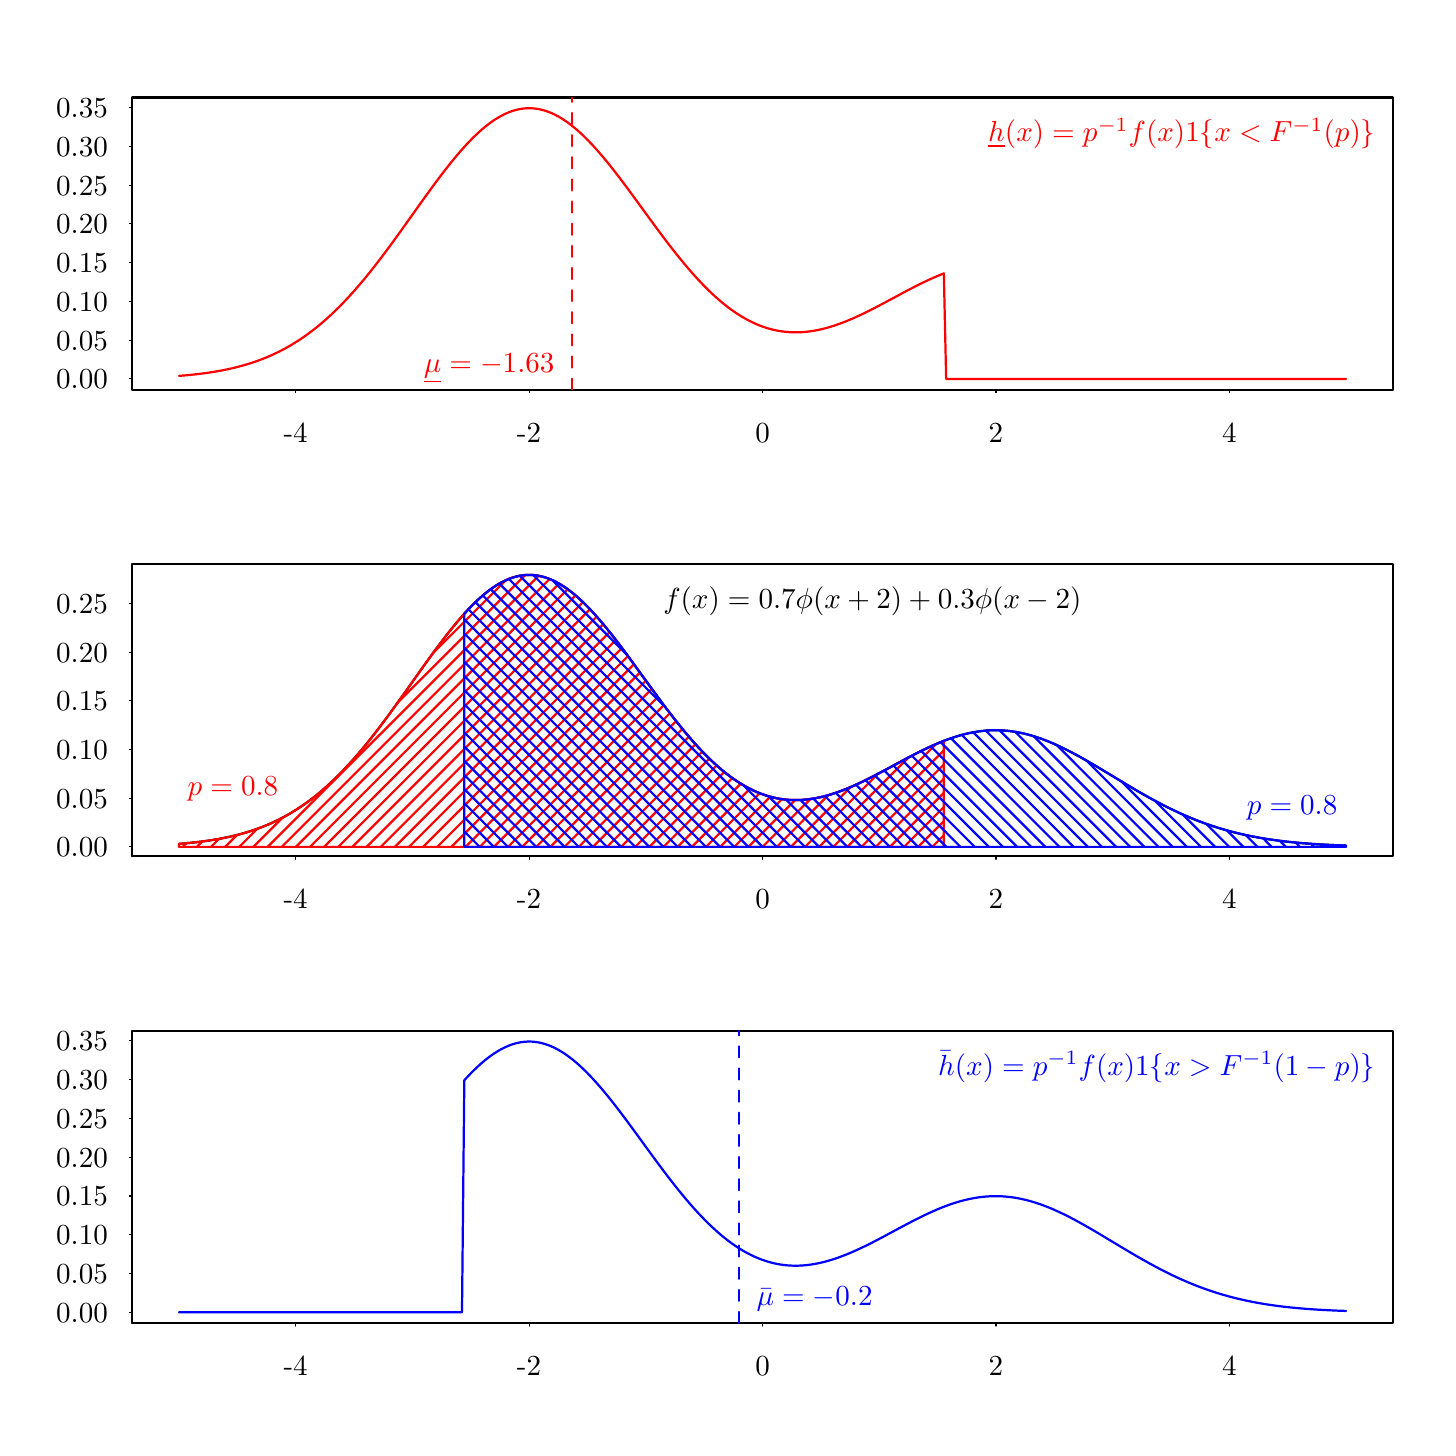
\begin{tikzpicture}[x=1pt,y=1pt]
\definecolor{fillColor}{RGB}{255,255,255}
\path[use as bounding box,fill=fillColor,fill opacity=0.00] (0,0) rectangle (505.89,505.89);
\begin{scope}
\path[clip] ( 37.80,375.06) rectangle (493.29,480.69);
\definecolor{drawColor}{RGB}{255,0,0}

\path[draw=drawColor,line width= 0.8pt,line join=round,line cap=round] ( 54.67,380.06) --
	( 55.52,380.13) --
	( 56.36,380.20) --
	( 57.21,380.27) --
	( 58.05,380.35) --
	( 58.90,380.43) --
	( 59.74,380.52) --
	( 60.59,380.61) --
	( 61.43,380.71) --
	( 62.28,380.81) --
	( 63.12,380.91) --
	( 63.97,381.03) --
	( 64.81,381.14) --
	( 65.66,381.27) --
	( 66.50,381.40) --
	( 67.35,381.53) --
	( 68.19,381.67) --
	( 69.04,381.82) --
	( 69.88,381.98) --
	( 70.73,382.14) --
	( 71.57,382.31) --
	( 72.42,382.49) --
	( 73.26,382.67) --
	( 74.11,382.87) --
	( 74.95,383.07) --
	( 75.80,383.28) --
	( 76.64,383.50) --
	( 77.49,383.73) --
	( 78.34,383.97) --
	( 79.18,384.22) --
	( 80.03,384.48) --
	( 80.87,384.75) --
	( 81.72,385.03) --
	( 82.56,385.32) --
	( 83.41,385.62) --
	( 84.25,385.94) --
	( 85.10,386.27) --
	( 85.94,386.60) --
	( 86.79,386.96) --
	( 87.63,387.32) --
	( 88.48,387.70) --
	( 89.32,388.09) --
	( 90.17,388.50) --
	( 91.01,388.91) --
	( 91.86,389.35) --
	( 92.70,389.79) --
	( 93.55,390.26) --
	( 94.39,390.73) --
	( 95.24,391.23) --
	( 96.08,391.74) --
	( 96.93,392.26) --
	( 97.77,392.80) --
	( 98.62,393.36) --
	( 99.47,393.93) --
	(100.31,394.52) --
	(101.16,395.12) --
	(102.00,395.75) --
	(102.85,396.39) --
	(103.69,397.04) --
	(104.54,397.72) --
	(105.38,398.41) --
	(106.23,399.12) --
	(107.07,399.84) --
	(107.92,400.59) --
	(108.76,401.35) --
	(109.61,402.13) --
	(110.45,402.93) --
	(111.30,403.74) --
	(112.14,404.57) --
	(112.99,405.42) --
	(113.83,406.28) --
	(114.68,407.17) --
	(115.52,408.07) --
	(116.37,408.98) --
	(117.21,409.92) --
	(118.06,410.86) --
	(118.90,411.83) --
	(119.75,412.81) --
	(120.59,413.80) --
	(121.44,414.82) --
	(122.29,415.84) --
	(123.13,416.88) --
	(123.98,417.93) --
	(124.82,419.00) --
	(125.67,420.08) --
	(126.51,421.17) --
	(127.36,422.27) --
	(128.20,423.38) --
	(129.05,424.50) --
	(129.89,425.64) --
	(130.74,426.78) --
	(131.58,427.93) --
	(132.43,429.09) --
	(133.27,430.25) --
	(134.12,431.42) --
	(134.96,432.60) --
	(135.81,433.78) --
	(136.65,434.96) --
	(137.50,436.15) --
	(138.34,437.34) --
	(139.19,438.52) --
	(140.03,439.71) --
	(140.88,440.90) --
	(141.72,442.09) --
	(142.57,443.27) --
	(143.41,444.45) --
	(144.26,445.62) --
	(145.11,446.78) --
	(145.95,447.94) --
	(146.80,449.09) --
	(147.64,450.24) --
	(148.49,451.37) --
	(149.33,452.49) --
	(150.18,453.59) --
	(151.02,454.68) --
	(151.87,455.76) --
	(152.71,456.82) --
	(153.56,457.87) --
	(154.40,458.90) --
	(155.25,459.90) --
	(156.09,460.89) --
	(156.94,461.86) --
	(157.78,462.80) --
	(158.63,463.72) --
	(159.47,464.62) --
	(160.32,465.49) --
	(161.16,466.34) --
	(162.01,467.15) --
	(162.85,467.94) --
	(163.70,468.71) --
	(164.54,469.44) --
	(165.39,470.14) --
	(166.24,470.81) --
	(167.08,471.44) --
	(167.93,472.05) --
	(168.77,472.62) --
	(169.62,473.15) --
	(170.46,473.65) --
	(171.31,474.12) --
	(172.15,474.55) --
	(173.00,474.94) --
	(173.84,475.30) --
	(174.69,475.62) --
	(175.53,475.90) --
	(176.38,476.14) --
	(177.22,476.34) --
	(178.07,476.51) --
	(178.91,476.63) --
	(179.76,476.72) --
	(180.60,476.77) --
	(181.45,476.78) --
	(182.29,476.75) --
	(183.14,476.68) --
	(183.98,476.57) --
	(184.83,476.42) --
	(185.67,476.24) --
	(186.52,476.01) --
	(187.36,475.75) --
	(188.21,475.45) --
	(189.06,475.11) --
	(189.90,474.74) --
	(190.75,474.32) --
	(191.59,473.88) --
	(192.44,473.39) --
	(193.28,472.87) --
	(194.13,472.32) --
	(194.97,471.73) --
	(195.82,471.11) --
	(196.66,470.46) --
	(197.51,469.78) --
	(198.35,469.06) --
	(199.20,468.32) --
	(200.04,467.55) --
	(200.89,466.75) --
	(201.73,465.92) --
	(202.58,465.06) --
	(203.42,464.18) --
	(204.27,463.28) --
	(205.11,462.35) --
	(205.96,461.40) --
	(206.80,460.43) --
	(207.65,459.44) --
	(208.49,458.43) --
	(209.34,457.41) --
	(210.19,456.36) --
	(211.03,455.30) --
	(211.88,454.23) --
	(212.72,453.14) --
	(213.57,452.04) --
	(214.41,450.93) --
	(215.26,449.81) --
	(216.10,448.68) --
	(216.95,447.54) --
	(217.79,446.40) --
	(218.64,445.24) --
	(219.48,444.09) --
	(220.33,442.93) --
	(221.17,441.77) --
	(222.02,440.61) --
	(222.86,439.45) --
	(223.71,438.29) --
	(224.55,437.13) --
	(225.40,435.97) --
	(226.24,434.82) --
	(227.09,433.67) --
	(227.93,432.53) --
	(228.78,431.40) --
	(229.62,430.27) --
	(230.47,429.15) --
	(231.31,428.04) --
	(232.16,426.94) --
	(233.01,425.86) --
	(233.85,424.78) --
	(234.70,423.72) --
	(235.54,422.67) --
	(236.39,421.63) --
	(237.23,420.61) --
	(238.08,419.60) --
	(238.92,418.61) --
	(239.77,417.64) --
	(240.61,416.68) --
	(241.46,415.74) --
	(242.30,414.82) --
	(243.15,413.92) --
	(243.99,413.04) --
	(244.84,412.18) --
	(245.68,411.33) --
	(246.53,410.51) --
	(247.37,409.71) --
	(248.22,408.93) --
	(249.06,408.17) --
	(249.91,407.43) --
	(250.75,406.71) --
	(251.60,406.02) --
	(252.44,405.35) --
	(253.29,404.70) --
	(254.13,404.07) --
	(254.98,403.47) --
	(255.83,402.89) --
	(256.67,402.33) --
	(257.52,401.80) --
	(258.36,401.29) --
	(259.21,400.80) --
	(260.05,400.33) --
	(260.90,399.89) --
	(261.74,399.48) --
	(262.59,399.08) --
	(263.43,398.71) --
	(264.28,398.36) --
	(265.12,398.03) --
	(265.97,397.73) --
	(266.81,397.45) --
	(267.66,397.19) --
	(268.50,396.96) --
	(269.35,396.74) --
	(270.19,396.55) --
	(271.04,396.38) --
	(271.88,396.24) --
	(272.73,396.11) --
	(273.57,396.01) --
	(274.42,395.92) --
	(275.26,395.86) --
	(276.11,395.82) --
	(276.96,395.79) --
	(277.80,395.79) --
	(278.65,395.81) --
	(279.49,395.84) --
	(280.34,395.90) --
	(281.18,395.97) --
	(282.03,396.07) --
	(282.87,396.18) --
	(283.72,396.30) --
	(284.56,396.45) --
	(285.41,396.61) --
	(286.25,396.79) --
	(287.10,396.98) --
	(287.94,397.19) --
	(288.79,397.42) --
	(289.63,397.66) --
	(290.48,397.92) --
	(291.32,398.18) --
	(292.17,398.47) --
	(293.01,398.76) --
	(293.86,399.07) --
	(294.70,399.39) --
	(295.55,399.72) --
	(296.39,400.06) --
	(297.24,400.42) --
	(298.08,400.78) --
	(298.93,401.15) --
	(299.78,401.54) --
	(300.62,401.93) --
	(301.47,402.33) --
	(302.31,402.73) --
	(303.16,403.15) --
	(304.00,403.57) --
	(304.85,403.99) --
	(305.69,404.42) --
	(306.54,404.86) --
	(307.38,405.30) --
	(308.23,405.75) --
	(309.07,406.19) --
	(309.92,406.64) --
	(310.76,407.10) --
	(311.61,407.55) --
	(312.45,408.00) --
	(313.30,408.46) --
	(314.14,408.91) --
	(314.99,409.37) --
	(315.83,409.82) --
	(316.68,410.27) --
	(317.52,410.72) --
	(318.37,411.16) --
	(319.21,411.60) --
	(320.06,412.04) --
	(320.90,412.47) --
	(321.75,412.90) --
	(322.60,413.32) --
	(323.44,413.73) --
	(324.29,414.14) --
	(325.13,414.54) --
	(325.98,414.93) --
	(326.82,415.31) --
	(327.67,415.68) --
	(328.51,416.05) --
	(329.36,416.40) --
	(330.20,416.75) --
	(331.05,417.08) --
	(331.89,378.97) --
	(332.74,378.97) --
	(333.58,378.97) --
	(334.43,378.97) --
	(335.27,378.97) --
	(336.12,378.97) --
	(336.96,378.97) --
	(337.81,378.97) --
	(338.65,378.97) --
	(339.50,378.97) --
	(340.34,378.97) --
	(341.19,378.97) --
	(342.03,378.97) --
	(342.88,378.97) --
	(343.73,378.97) --
	(344.57,378.97) --
	(345.42,378.97) --
	(346.26,378.97) --
	(347.11,378.97) --
	(347.95,378.97) --
	(348.80,378.97) --
	(349.64,378.97) --
	(350.49,378.97) --
	(351.33,378.97) --
	(352.18,378.97) --
	(353.02,378.97) --
	(353.87,378.97) --
	(354.71,378.97) --
	(355.56,378.97) --
	(356.40,378.97) --
	(357.25,378.97) --
	(358.09,378.97) --
	(358.94,378.97) --
	(359.78,378.97) --
	(360.63,378.97) --
	(361.47,378.97) --
	(362.32,378.97) --
	(363.16,378.97) --
	(364.01,378.97) --
	(364.85,378.97) --
	(365.70,378.97) --
	(366.55,378.97) --
	(367.39,378.97) --
	(368.24,378.97) --
	(369.08,378.97) --
	(369.93,378.97) --
	(370.77,378.97) --
	(371.62,378.97) --
	(372.46,378.97) --
	(373.31,378.97) --
	(374.15,378.97) --
	(375.00,378.97) --
	(375.84,378.97) --
	(376.69,378.97) --
	(377.53,378.97) --
	(378.38,378.97) --
	(379.22,378.97) --
	(380.07,378.97) --
	(380.91,378.97) --
	(381.76,378.97) --
	(382.60,378.97) --
	(383.45,378.97) --
	(384.29,378.97) --
	(385.14,378.97) --
	(385.98,378.97) --
	(386.83,378.97) --
	(387.68,378.97) --
	(388.52,378.97) --
	(389.37,378.97) --
	(390.21,378.97) --
	(391.06,378.97) --
	(391.90,378.97) --
	(392.75,378.97) --
	(393.59,378.97) --
	(394.44,378.97) --
	(395.28,378.97) --
	(396.13,378.97) --
	(396.97,378.97) --
	(397.82,378.97) --
	(398.66,378.97) --
	(399.51,378.97) --
	(400.35,378.97) --
	(401.20,378.97) --
	(402.04,378.97) --
	(402.89,378.97) --
	(403.73,378.97) --
	(404.58,378.97) --
	(405.42,378.97) --
	(406.27,378.97) --
	(407.11,378.97) --
	(407.96,378.97) --
	(408.80,378.97) --
	(409.65,378.97) --
	(410.50,378.97) --
	(411.34,378.97) --
	(412.19,378.97) --
	(413.03,378.97) --
	(413.88,378.97) --
	(414.72,378.97) --
	(415.57,378.97) --
	(416.41,378.97) --
	(417.26,378.97) --
	(418.10,378.97) --
	(418.95,378.97) --
	(419.79,378.97) --
	(420.64,378.97) --
	(421.48,378.97) --
	(422.33,378.97) --
	(423.17,378.97) --
	(424.02,378.97) --
	(424.86,378.97) --
	(425.71,378.97) --
	(426.55,378.97) --
	(427.40,378.97) --
	(428.24,378.97) --
	(429.09,378.97) --
	(429.93,378.97) --
	(430.78,378.97) --
	(431.62,378.97) --
	(432.47,378.97) --
	(433.32,378.97) --
	(434.16,378.97) --
	(435.01,378.97) --
	(435.85,378.97) --
	(436.70,378.97) --
	(437.54,378.97) --
	(438.39,378.97) --
	(439.23,378.97) --
	(440.08,378.97) --
	(440.92,378.97) --
	(441.77,378.97) --
	(442.61,378.97) --
	(443.46,378.97) --
	(444.30,378.97) --
	(445.15,378.97) --
	(445.99,378.97) --
	(446.84,378.97) --
	(447.68,378.97) --
	(448.53,378.97) --
	(449.37,378.97) --
	(450.22,378.97) --
	(451.06,378.97) --
	(451.91,378.97) --
	(452.75,378.97) --
	(453.60,378.97) --
	(454.45,378.97) --
	(455.29,378.97) --
	(456.14,378.97) --
	(456.98,378.97) --
	(457.83,378.97) --
	(458.67,378.97) --
	(459.52,378.97) --
	(460.36,378.97) --
	(461.21,378.97) --
	(462.05,378.97) --
	(462.90,378.97) --
	(463.74,378.97) --
	(464.59,378.97) --
	(465.43,378.97) --
	(466.28,378.97) --
	(467.12,378.97) --
	(467.97,378.97) --
	(468.81,378.97) --
	(469.66,378.97) --
	(470.50,378.97) --
	(471.35,378.97) --
	(472.19,378.97) --
	(473.04,378.97) --
	(473.88,378.97) --
	(474.73,378.97) --
	(475.57,378.97) --
	(476.42,378.97);
\end{scope}
\begin{scope}
\path[clip] (  0.00,  0.00) rectangle (505.89,505.89);
\definecolor{drawColor}{RGB}{0,0,0}

\path[draw=drawColor,line width= 0.4pt,line join=round,line cap=round] ( 96.84,375.06) -- (434.25,375.06);

\path[draw=drawColor,line width= 0.4pt,line join=round,line cap=round] ( 96.84,375.06) -- ( 96.84,374.00);

\path[draw=drawColor,line width= 0.4pt,line join=round,line cap=round] (181.19,375.06) -- (181.19,374.00);

\path[draw=drawColor,line width= 0.4pt,line join=round,line cap=round] (265.54,375.06) -- (265.54,374.00);

\path[draw=drawColor,line width= 0.4pt,line join=round,line cap=round] (349.89,375.06) -- (349.89,374.00);

\path[draw=drawColor,line width= 0.4pt,line join=round,line cap=round] (434.25,375.06) -- (434.25,374.00);

\node[text=drawColor,anchor=base,inner sep=0pt, outer sep=0pt, scale=  1.05] at ( 96.84,356.16) {-4};

\node[text=drawColor,anchor=base,inner sep=0pt, outer sep=0pt, scale=  1.05] at (181.19,356.16) {-2};

\node[text=drawColor,anchor=base,inner sep=0pt, outer sep=0pt, scale=  1.05] at (265.54,356.16) {0};

\node[text=drawColor,anchor=base,inner sep=0pt, outer sep=0pt, scale=  1.05] at (349.89,356.16) {2};

\node[text=drawColor,anchor=base,inner sep=0pt, outer sep=0pt, scale=  1.05] at (434.25,356.16) {4};

\path[draw=drawColor,line width= 0.4pt,line join=round,line cap=round] ( 37.80,378.97) -- ( 37.80,477.02);

\path[draw=drawColor,line width= 0.4pt,line join=round,line cap=round] ( 37.80,378.97) -- ( 36.74,378.97);

\path[draw=drawColor,line width= 0.4pt,line join=round,line cap=round] ( 37.80,392.98) -- ( 36.74,392.98);

\path[draw=drawColor,line width= 0.4pt,line join=round,line cap=round] ( 37.80,406.99) -- ( 36.74,406.99);

\path[draw=drawColor,line width= 0.4pt,line join=round,line cap=round] ( 37.80,420.99) -- ( 36.74,420.99);

\path[draw=drawColor,line width= 0.4pt,line join=round,line cap=round] ( 37.80,435.00) -- ( 36.74,435.00);

\path[draw=drawColor,line width= 0.4pt,line join=round,line cap=round] ( 37.80,449.01) -- ( 36.74,449.01);

\path[draw=drawColor,line width= 0.4pt,line join=round,line cap=round] ( 37.80,463.02) -- ( 36.74,463.02);

\path[draw=drawColor,line width= 0.4pt,line join=round,line cap=round] ( 37.80,477.02) -- ( 36.74,477.02);

\node[text=drawColor,anchor=base east,inner sep=0pt, outer sep=0pt, scale=  1.05] at ( 28.98,375.36) {0.00};

\node[text=drawColor,anchor=base east,inner sep=0pt, outer sep=0pt, scale=  1.05] at ( 28.98,389.36) {0.05};

\node[text=drawColor,anchor=base east,inner sep=0pt, outer sep=0pt, scale=  1.05] at ( 28.98,403.37) {0.10};

\node[text=drawColor,anchor=base east,inner sep=0pt, outer sep=0pt, scale=  1.05] at ( 28.98,417.38) {0.15};

\node[text=drawColor,anchor=base east,inner sep=0pt, outer sep=0pt, scale=  1.05] at ( 28.98,431.39) {0.20};

\node[text=drawColor,anchor=base east,inner sep=0pt, outer sep=0pt, scale=  1.05] at ( 28.98,445.39) {0.25};

\node[text=drawColor,anchor=base east,inner sep=0pt, outer sep=0pt, scale=  1.05] at ( 28.98,459.40) {0.30};

\node[text=drawColor,anchor=base east,inner sep=0pt, outer sep=0pt, scale=  1.05] at ( 28.98,473.41) {0.35};

\path[draw=drawColor,line width= 0.8pt,line join=round,line cap=round] ( 37.80,375.06) --
	(493.29,375.06) --
	(493.29,480.69) --
	( 37.80,480.69) --
	( 37.80,375.06);
\end{scope}
\begin{scope}
\path[clip] ( 37.80,375.06) rectangle (493.29,480.69);
\definecolor{drawColor}{RGB}{255,0,0}

\node[text=drawColor,anchor=base east,inner sep=0pt, outer sep=0pt, scale=  1.05] at (486.99,464.59) {$\underline{h}(x) = p^{-1}f(x) 1\{x < F^{-1}(p)\}$};

\path[draw=drawColor,line width= 0.8pt,dash pattern=on 4pt off 4pt ,line join=round,line cap=round] (196.63,375.06) -- (196.63,480.69);

\node[text=drawColor,anchor=base east,inner sep=0pt, outer sep=0pt, scale=  1.05] at (190.33,381.45) {$\underline{\mu} = -1.63$};
\end{scope}
\begin{scope}
\path[clip] ( 37.80,206.43) rectangle (493.29,312.06);
\definecolor{drawColor}{RGB}{0,0,0}

\path[draw=drawColor,line width= 0.8pt,line join=round,line cap=round] ( 54.67,210.97) --
	( 55.52,211.03) --
	( 56.36,211.10) --
	( 57.21,211.18) --
	( 58.05,211.26) --
	( 58.90,211.34) --
	( 59.74,211.43) --
	( 60.59,211.52) --
	( 61.43,211.62) --
	( 62.28,211.72) --
	( 63.12,211.83) --
	( 63.97,211.94) --
	( 64.81,212.06) --
	( 65.66,212.18) --
	( 66.50,212.31) --
	( 67.35,212.45) --
	( 68.19,212.59) --
	( 69.04,212.74) --
	( 69.88,212.89) --
	( 70.73,213.06) --
	( 71.57,213.23) --
	( 72.42,213.41) --
	( 73.26,213.59) --
	( 74.11,213.79) --
	( 74.95,213.99) --
	( 75.80,214.20) --
	( 76.64,214.42) --
	( 77.49,214.65) --
	( 78.34,214.90) --
	( 79.18,215.15) --
	( 80.03,215.41) --
	( 80.87,215.68) --
	( 81.72,215.96) --
	( 82.56,216.25) --
	( 83.41,216.56) --
	( 84.25,216.87) --
	( 85.10,217.20) --
	( 85.94,217.54) --
	( 86.79,217.90) --
	( 87.63,218.26) --
	( 88.48,218.64) --
	( 89.32,219.04) --
	( 90.17,219.44) --
	( 91.01,219.86) --
	( 91.86,220.30) --
	( 92.70,220.75) --
	( 93.55,221.21) --
	( 94.39,221.69) --
	( 95.24,222.19) --
	( 96.08,222.70) --
	( 96.93,223.23) --
	( 97.77,223.77) --
	( 98.62,224.33) --
	( 99.47,224.90) --
	(100.31,225.49) --
	(101.16,226.10) --
	(102.00,226.73) --
	(102.85,227.37) --
	(103.69,228.03) --
	(104.54,228.71) --
	(105.38,229.40) --
	(106.23,230.12) --
	(107.07,230.85) --
	(107.92,231.59) --
	(108.76,232.36) --
	(109.61,233.14) --
	(110.45,233.94) --
	(111.30,234.76) --
	(112.14,235.59) --
	(112.99,236.45) --
	(113.83,237.32) --
	(114.68,238.20) --
	(115.52,239.11) --
	(116.37,240.03) --
	(117.21,240.97) --
	(118.06,241.92) --
	(118.90,242.89) --
	(119.75,243.87) --
	(120.59,244.87) --
	(121.44,245.89) --
	(122.29,246.92) --
	(123.13,247.96) --
	(123.98,249.02) --
	(124.82,250.09) --
	(125.67,251.17) --
	(126.51,252.27) --
	(127.36,253.38) --
	(128.20,254.50) --
	(129.05,255.62) --
	(129.89,256.76) --
	(130.74,257.91) --
	(131.58,259.07) --
	(132.43,260.23) --
	(133.27,261.40) --
	(134.12,262.58) --
	(134.96,263.76) --
	(135.81,264.94) --
	(136.65,266.13) --
	(137.50,267.32) --
	(138.34,268.52) --
	(139.19,269.71) --
	(140.03,270.91) --
	(140.88,272.10) --
	(141.72,273.29) --
	(142.57,274.48) --
	(143.41,275.66) --
	(144.26,276.84) --
	(145.11,278.01) --
	(145.95,279.18) --
	(146.80,280.33) --
	(147.64,281.48) --
	(148.49,282.61) --
	(149.33,283.74) --
	(150.18,284.85) --
	(151.02,285.95) --
	(151.87,287.03) --
	(152.71,288.10) --
	(153.56,289.15) --
	(154.40,290.18) --
	(155.25,291.19) --
	(156.09,292.19) --
	(156.94,293.16) --
	(157.78,294.11) --
	(158.63,295.03) --
	(159.47,295.93) --
	(160.32,296.81) --
	(161.16,297.66) --
	(162.01,298.48) --
	(162.85,299.27) --
	(163.70,300.04) --
	(164.54,300.77) --
	(165.39,301.47) --
	(166.24,302.15) --
	(167.08,302.79) --
	(167.93,303.39) --
	(168.77,303.97) --
	(169.62,304.51) --
	(170.46,305.01) --
	(171.31,305.48) --
	(172.15,305.91) --
	(173.00,306.30) --
	(173.84,306.66) --
	(174.69,306.98) --
	(175.53,307.26) --
	(176.38,307.50) --
	(177.22,307.71) --
	(178.07,307.88) --
	(178.91,308.00) --
	(179.76,308.09) --
	(180.60,308.14) --
	(181.45,308.15) --
	(182.29,308.12) --
	(183.14,308.05) --
	(183.98,307.94) --
	(184.83,307.79) --
	(185.67,307.60) --
	(186.52,307.38) --
	(187.36,307.11) --
	(188.21,306.81) --
	(189.06,306.47) --
	(189.90,306.10) --
	(190.75,305.68) --
	(191.59,305.23) --
	(192.44,304.75) --
	(193.28,304.22) --
	(194.13,303.67) --
	(194.97,303.08) --
	(195.82,302.46) --
	(196.66,301.80) --
	(197.51,301.12) --
	(198.35,300.40) --
	(199.20,299.65) --
	(200.04,298.87) --
	(200.89,298.07) --
	(201.73,297.24) --
	(202.58,296.38) --
	(203.42,295.49) --
	(204.27,294.59) --
	(205.11,293.65) --
	(205.96,292.70) --
	(206.80,291.73) --
	(207.65,290.73) --
	(208.49,289.72) --
	(209.34,288.68) --
	(210.19,287.63) --
	(211.03,286.57) --
	(211.88,285.49) --
	(212.72,284.40) --
	(213.57,283.29) --
	(214.41,282.18) --
	(215.26,281.05) --
	(216.10,279.91) --
	(216.95,278.77) --
	(217.79,277.62) --
	(218.64,276.46) --
	(219.48,275.30) --
	(220.33,274.14) --
	(221.17,272.97) --
	(222.02,271.81) --
	(222.86,270.64) --
	(223.71,269.47) --
	(224.55,268.31) --
	(225.40,267.15) --
	(226.24,265.99) --
	(227.09,264.84) --
	(227.93,263.69) --
	(228.78,262.55) --
	(229.62,261.42) --
	(230.47,260.29) --
	(231.31,259.18) --
	(232.16,258.08) --
	(233.01,256.98) --
	(233.85,255.90) --
	(234.70,254.83) --
	(235.54,253.78) --
	(236.39,252.74) --
	(237.23,251.71) --
	(238.08,250.70) --
	(238.92,249.71) --
	(239.77,248.73) --
	(240.61,247.77) --
	(241.46,246.82) --
	(242.30,245.90) --
	(243.15,244.99) --
	(243.99,244.10) --
	(244.84,243.24) --
	(245.68,242.39) --
	(246.53,241.56) --
	(247.37,240.76) --
	(248.22,239.97) --
	(249.06,239.21) --
	(249.91,238.47) --
	(250.75,237.75) --
	(251.60,237.05) --
	(252.44,236.38) --
	(253.29,235.73) --
	(254.13,235.10) --
	(254.98,234.49) --
	(255.83,233.91) --
	(256.67,233.35) --
	(257.52,232.81) --
	(258.36,232.30) --
	(259.21,231.81) --
	(260.05,231.34) --
	(260.90,230.90) --
	(261.74,230.48) --
	(262.59,230.08) --
	(263.43,229.70) --
	(264.28,229.35) --
	(265.12,229.03) --
	(265.97,228.72) --
	(266.81,228.44) --
	(267.66,228.18) --
	(268.50,227.94) --
	(269.35,227.73) --
	(270.19,227.54) --
	(271.04,227.37) --
	(271.88,227.22) --
	(272.73,227.09) --
	(273.57,226.99) --
	(274.42,226.90) --
	(275.26,226.84) --
	(276.11,226.80) --
	(276.96,226.78) --
	(277.80,226.77) --
	(278.65,226.79) --
	(279.49,226.83) --
	(280.34,226.88) --
	(281.18,226.96) --
	(282.03,227.05) --
	(282.87,227.16) --
	(283.72,227.29) --
	(284.56,227.44) --
	(285.41,227.60) --
	(286.25,227.78) --
	(287.10,227.97) --
	(287.94,228.18) --
	(288.79,228.41) --
	(289.63,228.65) --
	(290.48,228.91) --
	(291.32,229.18) --
	(292.17,229.46) --
	(293.01,229.76) --
	(293.86,230.07) --
	(294.70,230.39) --
	(295.55,230.72) --
	(296.39,231.07) --
	(297.24,231.42) --
	(298.08,231.79) --
	(298.93,232.16) --
	(299.78,232.55) --
	(300.62,232.94) --
	(301.47,233.34) --
	(302.31,233.75) --
	(303.16,234.16) --
	(304.00,234.59) --
	(304.85,235.01) --
	(305.69,235.45) --
	(306.54,235.89) --
	(307.38,236.33) --
	(308.23,236.78) --
	(309.07,237.23) --
	(309.92,237.68) --
	(310.76,238.13) --
	(311.61,238.59) --
	(312.45,239.05) --
	(313.30,239.50) --
	(314.14,239.96) --
	(314.99,240.41) --
	(315.83,240.87) --
	(316.68,241.32) --
	(317.52,241.77) --
	(318.37,242.22) --
	(319.21,242.66) --
	(320.06,243.10) --
	(320.90,243.53) --
	(321.75,243.96) --
	(322.60,244.38) --
	(323.44,244.80) --
	(324.29,245.21) --
	(325.13,245.61) --
	(325.98,246.00) --
	(326.82,246.39) --
	(327.67,246.76) --
	(328.51,247.13) --
	(329.36,247.48) --
	(330.20,247.83) --
	(331.05,248.16) --
	(331.89,248.49) --
	(332.74,248.80) --
	(333.58,249.09) --
	(334.43,249.38) --
	(335.27,249.65) --
	(336.12,249.91) --
	(336.96,250.16) --
	(337.81,250.39) --
	(338.65,250.61) --
	(339.50,250.81) --
	(340.34,251.00) --
	(341.19,251.17) --
	(342.03,251.33) --
	(342.88,251.47) --
	(343.73,251.60) --
	(344.57,251.71) --
	(345.42,251.80) --
	(346.26,251.88) --
	(347.11,251.94) --
	(347.95,251.98) --
	(348.80,252.01) --
	(349.64,252.02) --
	(350.49,252.01) --
	(351.33,251.99) --
	(352.18,251.95) --
	(353.02,251.89) --
	(353.87,251.82) --
	(354.71,251.73) --
	(355.56,251.63) --
	(356.40,251.51) --
	(357.25,251.37) --
	(358.09,251.21) --
	(358.94,251.04) --
	(359.78,250.86) --
	(360.63,250.66) --
	(361.47,250.44) --
	(362.32,250.21) --
	(363.16,249.96) --
	(364.01,249.70) --
	(364.85,249.43) --
	(365.70,249.14) --
	(366.55,248.84) --
	(367.39,248.52) --
	(368.24,248.19) --
	(369.08,247.85) --
	(369.93,247.50) --
	(370.77,247.13) --
	(371.62,246.76) --
	(372.46,246.37) --
	(373.31,245.98) --
	(374.15,245.57) --
	(375.00,245.15) --
	(375.84,244.73) --
	(376.69,244.29) --
	(377.53,243.85) --
	(378.38,243.40) --
	(379.22,242.94) --
	(380.07,242.48) --
	(380.91,242.01) --
	(381.76,241.53) --
	(382.60,241.05) --
	(383.45,240.56) --
	(384.29,240.07) --
	(385.14,239.58) --
	(385.98,239.08) --
	(386.83,238.57) --
	(387.68,238.07) --
	(388.52,237.56) --
	(389.37,237.05) --
	(390.21,236.54) --
	(391.06,236.03) --
	(391.90,235.52) --
	(392.75,235.01) --
	(393.59,234.50) --
	(394.44,233.98) --
	(395.28,233.48) --
	(396.13,232.97) --
	(396.97,232.46) --
	(397.82,231.96) --
	(398.66,231.46) --
	(399.51,230.96) --
	(400.35,230.46) --
	(401.20,229.97) --
	(402.04,229.48) --
	(402.89,229.00) --
	(403.73,228.52) --
	(404.58,228.04) --
	(405.42,227.57) --
	(406.27,227.11) --
	(407.11,226.65) --
	(407.96,226.20) --
	(408.80,225.75) --
	(409.65,225.31) --
	(410.50,224.87) --
	(411.34,224.45) --
	(412.19,224.02) --
	(413.03,223.61) --
	(413.88,223.20) --
	(414.72,222.80) --
	(415.57,222.40) --
	(416.41,222.02) --
	(417.26,221.64) --
	(418.10,221.26) --
	(418.95,220.90) --
	(419.79,220.54) --
	(420.64,220.19) --
	(421.48,219.85) --
	(422.33,219.51) --
	(423.17,219.18) --
	(424.02,218.86) --
	(424.86,218.55) --
	(425.71,218.24) --
	(426.55,217.95) --
	(427.40,217.66) --
	(428.24,217.37) --
	(429.09,217.10) --
	(429.93,216.83) --
	(430.78,216.57) --
	(431.62,216.32) --
	(432.47,216.07) --
	(433.32,215.83) --
	(434.16,215.60) --
	(435.01,215.37) --
	(435.85,215.15) --
	(436.70,214.94) --
	(437.54,214.73) --
	(438.39,214.53) --
	(439.23,214.34) --
	(440.08,214.16) --
	(440.92,213.98) --
	(441.77,213.80) --
	(442.61,213.63) --
	(443.46,213.47) --
	(444.30,213.31) --
	(445.15,213.16) --
	(445.99,213.02) --
	(446.84,212.87) --
	(447.68,212.74) --
	(448.53,212.61) --
	(449.37,212.48) --
	(450.22,212.36) --
	(451.06,212.25) --
	(451.91,212.13) --
	(452.75,212.03) --
	(453.60,211.92) --
	(454.45,211.82) --
	(455.29,211.73) --
	(456.14,211.64) --
	(456.98,211.55) --
	(457.83,211.47) --
	(458.67,211.39) --
	(459.52,211.31) --
	(460.36,211.24) --
	(461.21,211.17) --
	(462.05,211.10) --
	(462.90,211.04) --
	(463.74,210.98) --
	(464.59,210.92) --
	(465.43,210.86) --
	(466.28,210.81) --
	(467.12,210.76) --
	(467.97,210.71) --
	(468.81,210.67) --
	(469.66,210.62) --
	(470.50,210.58) --
	(471.35,210.54) --
	(472.19,210.50) --
	(473.04,210.47) --
	(473.88,210.43) --
	(474.73,210.40) --
	(475.57,210.37) --
	(476.42,210.34);
\end{scope}
\begin{scope}
\path[clip] (  0.00,  0.00) rectangle (505.89,505.89);
\definecolor{drawColor}{RGB}{0,0,0}

\path[draw=drawColor,line width= 0.4pt,line join=round,line cap=round] ( 96.84,206.43) -- (434.25,206.43);

\path[draw=drawColor,line width= 0.4pt,line join=round,line cap=round] ( 96.84,206.43) -- ( 96.84,205.37);

\path[draw=drawColor,line width= 0.4pt,line join=round,line cap=round] (181.19,206.43) -- (181.19,205.37);

\path[draw=drawColor,line width= 0.4pt,line join=round,line cap=round] (265.54,206.43) -- (265.54,205.37);

\path[draw=drawColor,line width= 0.4pt,line join=round,line cap=round] (349.89,206.43) -- (349.89,205.37);

\path[draw=drawColor,line width= 0.4pt,line join=round,line cap=round] (434.25,206.43) -- (434.25,205.37);

\node[text=drawColor,anchor=base,inner sep=0pt, outer sep=0pt, scale=  1.05] at ( 96.84,187.53) {-4};

\node[text=drawColor,anchor=base,inner sep=0pt, outer sep=0pt, scale=  1.05] at (181.19,187.53) {-2};

\node[text=drawColor,anchor=base,inner sep=0pt, outer sep=0pt, scale=  1.05] at (265.54,187.53) {0};

\node[text=drawColor,anchor=base,inner sep=0pt, outer sep=0pt, scale=  1.05] at (349.89,187.53) {2};

\node[text=drawColor,anchor=base,inner sep=0pt, outer sep=0pt, scale=  1.05] at (434.25,187.53) {4};

\path[draw=drawColor,line width= 0.4pt,line join=round,line cap=round] ( 37.80,209.87) -- ( 37.80,297.84);

\path[draw=drawColor,line width= 0.4pt,line join=round,line cap=round] ( 37.80,209.87) -- ( 36.74,209.87);

\path[draw=drawColor,line width= 0.4pt,line join=round,line cap=round] ( 37.80,227.47) -- ( 36.74,227.47);

\path[draw=drawColor,line width= 0.4pt,line join=round,line cap=round] ( 37.80,245.06) -- ( 36.74,245.06);

\path[draw=drawColor,line width= 0.4pt,line join=round,line cap=round] ( 37.80,262.65) -- ( 36.74,262.65);

\path[draw=drawColor,line width= 0.4pt,line join=round,line cap=round] ( 37.80,280.25) -- ( 36.74,280.25);

\path[draw=drawColor,line width= 0.4pt,line join=round,line cap=round] ( 37.80,297.84) -- ( 36.74,297.84);

\node[text=drawColor,anchor=base east,inner sep=0pt, outer sep=0pt, scale=  1.05] at ( 28.98,206.26) {0.00};

\node[text=drawColor,anchor=base east,inner sep=0pt, outer sep=0pt, scale=  1.05] at ( 28.98,223.85) {0.05};

\node[text=drawColor,anchor=base east,inner sep=0pt, outer sep=0pt, scale=  1.05] at ( 28.98,241.44) {0.10};

\node[text=drawColor,anchor=base east,inner sep=0pt, outer sep=0pt, scale=  1.05] at ( 28.98,259.04) {0.15};

\node[text=drawColor,anchor=base east,inner sep=0pt, outer sep=0pt, scale=  1.05] at ( 28.98,276.63) {0.20};

\node[text=drawColor,anchor=base east,inner sep=0pt, outer sep=0pt, scale=  1.05] at ( 28.98,294.22) {0.25};

\path[draw=drawColor,line width= 0.8pt,line join=round,line cap=round] ( 37.80,206.43) --
	(493.29,206.43) --
	(493.29,312.06) --
	( 37.80,312.06) --
	( 37.80,206.43);
\end{scope}
\begin{scope}
\path[clip] ( 37.80,206.43) rectangle (493.29,312.06);
\definecolor{drawColor}{RGB}{255,0,0}

\path[draw=drawColor,line width= 0.8pt,line join=round,line cap=round] ( 56.02,209.87) -- ( 57.34,211.19);

\path[draw=drawColor,line width= 0.8pt,line join=round,line cap=round] ( 61.13,209.87) -- ( 63.08,211.82);

\path[draw=drawColor,line width= 0.8pt,line join=round,line cap=round] ( 66.24,209.87) -- ( 69.12,212.75);

\path[draw=drawColor,line width= 0.8pt,line join=round,line cap=round] ( 71.36,209.87) -- ( 75.64,214.16);

\path[draw=drawColor,line width= 0.8pt,line join=round,line cap=round] ( 76.47,209.87) -- ( 83.00,216.41);

\path[draw=drawColor,line width= 0.8pt,line join=round,line cap=round] (146.45,279.86) -- (172.80,306.21);

\path[draw=drawColor,line width= 0.8pt,line join=round,line cap=round] ( 81.58,209.87) -- ( 92.16,220.46);

\path[draw=drawColor,line width= 0.8pt,line join=round,line cap=round] (133.71,262.01) -- (179.79,308.09);

\path[draw=drawColor,line width= 0.8pt,line join=round,line cap=round] ( 86.69,209.87) -- (184.64,307.82);

\path[draw=drawColor,line width= 0.8pt,line join=round,line cap=round] ( 91.80,209.87) -- (188.58,306.66);

\path[draw=drawColor,line width= 0.8pt,line join=round,line cap=round] ( 96.91,209.87) -- (192.02,304.99);

\path[draw=drawColor,line width= 0.8pt,line join=round,line cap=round] (102.02,209.87) -- (195.12,302.97);

\path[draw=drawColor,line width= 0.8pt,line join=round,line cap=round] (107.13,209.87) -- (197.97,300.72);

\path[draw=drawColor,line width= 0.8pt,line join=round,line cap=round] (112.24,209.87) -- (200.65,298.29);

\path[draw=drawColor,line width= 0.8pt,line join=round,line cap=round] (117.35,209.87) -- (203.20,295.73);

\path[draw=drawColor,line width= 0.8pt,line join=round,line cap=round] (122.46,209.87) -- (205.64,293.06);

\path[draw=drawColor,line width= 0.8pt,line join=round,line cap=round] (127.57,209.87) -- (208.00,290.31);

\path[draw=drawColor,line width= 0.8pt,line join=round,line cap=round] (132.68,209.87) -- (210.30,287.49);

\path[draw=drawColor,line width= 0.8pt,line join=round,line cap=round] (137.79,209.87) -- (212.54,284.63);

\path[draw=drawColor,line width= 0.8pt,line join=round,line cap=round] (142.90,209.87) -- (214.75,281.72);

\path[draw=drawColor,line width= 0.8pt,line join=round,line cap=round] (148.01,209.87) -- (216.93,278.79);

\path[draw=drawColor,line width= 0.8pt,line join=round,line cap=round] (153.12,209.87) -- (219.09,275.84);

\path[draw=drawColor,line width= 0.8pt,line join=round,line cap=round] (158.23,209.87) -- (221.24,272.88);

\path[draw=drawColor,line width= 0.8pt,line join=round,line cap=round] (163.34,209.87) -- (223.39,269.92);

\path[draw=drawColor,line width= 0.8pt,line join=round,line cap=round] (168.45,209.87) -- (225.54,266.96);

\path[draw=drawColor,line width= 0.8pt,line join=round,line cap=round] (173.56,209.87) -- (227.70,264.01);

\path[draw=drawColor,line width= 0.8pt,line join=round,line cap=round] (178.67,209.87) -- (229.88,261.08);

\path[draw=drawColor,line width= 0.8pt,line join=round,line cap=round] (183.78,209.87) -- (232.08,258.18);

\path[draw=drawColor,line width= 0.8pt,line join=round,line cap=round] (188.89,209.87) -- (234.32,255.31);

\path[draw=drawColor,line width= 0.8pt,line join=round,line cap=round] (194.00,209.87) -- (236.60,252.47);

\path[draw=drawColor,line width= 0.8pt,line join=round,line cap=round] (199.11,209.87) -- (238.93,249.69);

\path[draw=drawColor,line width= 0.8pt,line join=round,line cap=round] (204.22,209.87) -- (241.32,246.97);

\path[draw=drawColor,line width= 0.8pt,line join=round,line cap=round] (209.33,209.87) -- (243.78,244.32);

\path[draw=drawColor,line width= 0.8pt,line join=round,line cap=round] (214.44,209.87) -- (246.33,241.76);

\path[draw=drawColor,line width= 0.8pt,line join=round,line cap=round] (219.55,209.87) -- (248.97,239.29);

\path[draw=drawColor,line width= 0.8pt,line join=round,line cap=round] (224.66,209.87) -- (251.73,236.95);

\path[draw=drawColor,line width= 0.8pt,line join=round,line cap=round] (229.77,209.87) -- (254.64,234.74);

\path[draw=drawColor,line width= 0.8pt,line join=round,line cap=round] (234.88,209.87) -- (257.70,232.70);

\path[draw=drawColor,line width= 0.8pt,line join=round,line cap=round] (239.99,209.87) -- (260.98,230.86);

\path[draw=drawColor,line width= 0.8pt,line join=round,line cap=round] (245.10,209.87) -- (264.50,229.27);

\path[draw=drawColor,line width= 0.8pt,line join=round,line cap=round] (250.21,209.87) -- (268.33,227.99);

\path[draw=drawColor,line width= 0.8pt,line join=round,line cap=round] (255.32,209.87) -- (272.57,227.12);

\path[draw=drawColor,line width= 0.8pt,line join=round,line cap=round] (260.43,209.87) -- (277.34,226.77);

\path[draw=drawColor,line width= 0.8pt,line join=round,line cap=round] (265.54,209.87) -- (282.83,227.15);

\path[draw=drawColor,line width= 0.8pt,line join=round,line cap=round] (270.66,209.87) -- (289.35,228.57);

\path[draw=drawColor,line width= 0.8pt,line join=round,line cap=round] (275.77,209.87) -- (297.37,231.48);

\path[draw=drawColor,line width= 0.8pt,line join=round,line cap=round] (280.88,209.87) -- (307.28,236.27);

\path[draw=drawColor,line width= 0.8pt,line join=round,line cap=round] (285.99,209.87) -- (318.28,242.17);

\path[draw=drawColor,line width= 0.8pt,line join=round,line cap=round] (291.10,209.87) -- (328.22,247.00);

\path[draw=drawColor,line width= 0.8pt,line join=round,line cap=round] (296.21,209.87) -- (331.05,244.72);

\path[draw=drawColor,line width= 0.8pt,line join=round,line cap=round] (301.32,209.87) -- (331.05,239.60);

\path[draw=drawColor,line width= 0.8pt,line join=round,line cap=round] (306.43,209.87) -- (331.05,234.49);

\path[draw=drawColor,line width= 0.8pt,line join=round,line cap=round] (311.54,209.87) -- (331.05,229.38);

\path[draw=drawColor,line width= 0.8pt,line join=round,line cap=round] (316.65,209.87) -- (331.05,224.27);

\path[draw=drawColor,line width= 0.8pt,line join=round,line cap=round] (321.76,209.87) -- (331.05,219.16);

\path[draw=drawColor,line width= 0.8pt,line join=round,line cap=round] (326.87,209.87) -- (331.05,214.05);

\path[draw=drawColor,line width= 0.8pt,line join=round,line cap=round] ( 54.67,209.87) --
	( 55.52,209.87) --
	( 56.36,209.87) --
	( 57.21,209.87) --
	( 58.05,209.87) --
	( 58.90,209.87) --
	( 59.74,209.87) --
	( 60.59,209.87) --
	( 61.43,209.87) --
	( 62.28,209.87) --
	( 63.12,209.87) --
	( 63.97,209.87) --
	( 64.81,209.87) --
	( 65.66,209.87) --
	( 66.50,209.87) --
	( 67.35,209.87) --
	( 68.19,209.87) --
	( 69.04,209.87) --
	( 69.88,209.87) --
	( 70.73,209.87) --
	( 71.57,209.87) --
	( 72.42,209.87) --
	( 73.26,209.87) --
	( 74.11,209.87) --
	( 74.95,209.87) --
	( 75.80,209.87) --
	( 76.64,209.87) --
	( 77.49,209.87) --
	( 78.34,209.87) --
	( 79.18,209.87) --
	( 80.03,209.87) --
	( 80.87,209.87) --
	( 81.72,209.87) --
	( 82.56,209.87) --
	( 83.41,209.87) --
	( 84.25,209.87) --
	( 85.10,209.87) --
	( 85.94,209.87) --
	( 86.79,209.87) --
	( 87.63,209.87) --
	( 88.48,209.87) --
	( 89.32,209.87) --
	( 90.17,209.87) --
	( 91.01,209.87) --
	( 91.86,209.87) --
	( 92.70,209.87) --
	( 93.55,209.87) --
	( 94.39,209.87) --
	( 95.24,209.87) --
	( 96.08,209.87) --
	( 96.93,209.87) --
	( 97.77,209.87) --
	( 98.62,209.87) --
	( 99.47,209.87) --
	(100.31,209.87) --
	(101.16,209.87) --
	(102.00,209.87) --
	(102.85,209.87) --
	(103.69,209.87) --
	(104.54,209.87) --
	(105.38,209.87) --
	(106.23,209.87) --
	(107.07,209.87) --
	(107.92,209.87) --
	(108.76,209.87) --
	(109.61,209.87) --
	(110.45,209.87) --
	(111.30,209.87) --
	(112.14,209.87) --
	(112.99,209.87) --
	(113.83,209.87) --
	(114.68,209.87) --
	(115.52,209.87) --
	(116.37,209.87) --
	(117.21,209.87) --
	(118.06,209.87) --
	(118.90,209.87) --
	(119.75,209.87) --
	(120.59,209.87) --
	(121.44,209.87) --
	(122.29,209.87) --
	(123.13,209.87) --
	(123.98,209.87) --
	(124.82,209.87) --
	(125.67,209.87) --
	(126.51,209.87) --
	(127.36,209.87) --
	(128.20,209.87) --
	(129.05,209.87) --
	(129.89,209.87) --
	(130.74,209.87) --
	(131.58,209.87) --
	(132.43,209.87) --
	(133.27,209.87) --
	(134.12,209.87) --
	(134.96,209.87) --
	(135.81,209.87) --
	(136.65,209.87) --
	(137.50,209.87) --
	(138.34,209.87) --
	(139.19,209.87) --
	(140.03,209.87) --
	(140.88,209.87) --
	(141.72,209.87) --
	(142.57,209.87) --
	(143.41,209.87) --
	(144.26,209.87) --
	(145.11,209.87) --
	(145.95,209.87) --
	(146.80,209.87) --
	(147.64,209.87) --
	(148.49,209.87) --
	(149.33,209.87) --
	(150.18,209.87) --
	(151.02,209.87) --
	(151.87,209.87) --
	(152.71,209.87) --
	(153.56,209.87) --
	(154.40,209.87) --
	(155.25,209.87) --
	(156.09,209.87) --
	(156.94,209.87) --
	(157.78,209.87) --
	(158.63,209.87) --
	(159.47,209.87) --
	(160.32,209.87) --
	(161.16,209.87) --
	(162.01,209.87) --
	(162.85,209.87) --
	(163.70,209.87) --
	(164.54,209.87) --
	(165.39,209.87) --
	(166.24,209.87) --
	(167.08,209.87) --
	(167.93,209.87) --
	(168.77,209.87) --
	(169.62,209.87) --
	(170.46,209.87) --
	(171.31,209.87) --
	(172.15,209.87) --
	(173.00,209.87) --
	(173.84,209.87) --
	(174.69,209.87) --
	(175.53,209.87) --
	(176.38,209.87) --
	(177.22,209.87) --
	(178.07,209.87) --
	(178.91,209.87) --
	(179.76,209.87) --
	(180.60,209.87) --
	(181.45,209.87) --
	(182.29,209.87) --
	(183.14,209.87) --
	(183.98,209.87) --
	(184.83,209.87) --
	(185.67,209.87) --
	(186.52,209.87) --
	(187.36,209.87) --
	(188.21,209.87) --
	(189.06,209.87) --
	(189.90,209.87) --
	(190.75,209.87) --
	(191.59,209.87) --
	(192.44,209.87) --
	(193.28,209.87) --
	(194.13,209.87) --
	(194.97,209.87) --
	(195.82,209.87) --
	(196.66,209.87) --
	(197.51,209.87) --
	(198.35,209.87) --
	(199.20,209.87) --
	(200.04,209.87) --
	(200.89,209.87) --
	(201.73,209.87) --
	(202.58,209.87) --
	(203.42,209.87) --
	(204.27,209.87) --
	(205.11,209.87) --
	(205.96,209.87) --
	(206.80,209.87) --
	(207.65,209.87) --
	(208.49,209.87) --
	(209.34,209.87) --
	(210.19,209.87) --
	(211.03,209.87) --
	(211.88,209.87) --
	(212.72,209.87) --
	(213.57,209.87) --
	(214.41,209.87) --
	(215.26,209.87) --
	(216.10,209.87) --
	(216.95,209.87) --
	(217.79,209.87) --
	(218.64,209.87) --
	(219.48,209.87) --
	(220.33,209.87) --
	(221.17,209.87) --
	(222.02,209.87) --
	(222.86,209.87) --
	(223.71,209.87) --
	(224.55,209.87) --
	(225.40,209.87) --
	(226.24,209.87) --
	(227.09,209.87) --
	(227.93,209.87) --
	(228.78,209.87) --
	(229.62,209.87) --
	(230.47,209.87) --
	(231.31,209.87) --
	(232.16,209.87) --
	(233.01,209.87) --
	(233.85,209.87) --
	(234.70,209.87) --
	(235.54,209.87) --
	(236.39,209.87) --
	(237.23,209.87) --
	(238.08,209.87) --
	(238.92,209.87) --
	(239.77,209.87) --
	(240.61,209.87) --
	(241.46,209.87) --
	(242.30,209.87) --
	(243.15,209.87) --
	(243.99,209.87) --
	(244.84,209.87) --
	(245.68,209.87) --
	(246.53,209.87) --
	(247.37,209.87) --
	(248.22,209.87) --
	(249.06,209.87) --
	(249.91,209.87) --
	(250.75,209.87) --
	(251.60,209.87) --
	(252.44,209.87) --
	(253.29,209.87) --
	(254.13,209.87) --
	(254.98,209.87) --
	(255.83,209.87) --
	(256.67,209.87) --
	(257.52,209.87) --
	(258.36,209.87) --
	(259.21,209.87) --
	(260.05,209.87) --
	(260.90,209.87) --
	(261.74,209.87) --
	(262.59,209.87) --
	(263.43,209.87) --
	(264.28,209.87) --
	(265.12,209.87) --
	(265.97,209.87) --
	(266.81,209.87) --
	(267.66,209.87) --
	(268.50,209.87) --
	(269.35,209.87) --
	(270.19,209.87) --
	(271.04,209.87) --
	(271.88,209.87) --
	(272.73,209.87) --
	(273.57,209.87) --
	(274.42,209.87) --
	(275.26,209.87) --
	(276.11,209.87) --
	(276.96,209.87) --
	(277.80,209.87) --
	(278.65,209.87) --
	(279.49,209.87) --
	(280.34,209.87) --
	(281.18,209.87) --
	(282.03,209.87) --
	(282.87,209.87) --
	(283.72,209.87) --
	(284.56,209.87) --
	(285.41,209.87) --
	(286.25,209.87) --
	(287.10,209.87) --
	(287.94,209.87) --
	(288.79,209.87) --
	(289.63,209.87) --
	(290.48,209.87) --
	(291.32,209.87) --
	(292.17,209.87) --
	(293.01,209.87) --
	(293.86,209.87) --
	(294.70,209.87) --
	(295.55,209.87) --
	(296.39,209.87) --
	(297.24,209.87) --
	(298.08,209.87) --
	(298.93,209.87) --
	(299.78,209.87) --
	(300.62,209.87) --
	(301.47,209.87) --
	(302.31,209.87) --
	(303.16,209.87) --
	(304.00,209.87) --
	(304.85,209.87) --
	(305.69,209.87) --
	(306.54,209.87) --
	(307.38,209.87) --
	(308.23,209.87) --
	(309.07,209.87) --
	(309.92,209.87) --
	(310.76,209.87) --
	(311.61,209.87) --
	(312.45,209.87) --
	(313.30,209.87) --
	(314.14,209.87) --
	(314.99,209.87) --
	(315.83,209.87) --
	(316.68,209.87) --
	(317.52,209.87) --
	(318.37,209.87) --
	(319.21,209.87) --
	(320.06,209.87) --
	(320.90,209.87) --
	(321.75,209.87) --
	(322.60,209.87) --
	(323.44,209.87) --
	(324.29,209.87) --
	(325.13,209.87) --
	(325.98,209.87) --
	(326.82,209.87) --
	(327.67,209.87) --
	(328.51,209.87) --
	(329.36,209.87) --
	(330.20,209.87) --
	(331.05,209.87) --
	(331.05,248.16) --
	(330.20,247.83) --
	(329.36,247.48) --
	(328.51,247.13) --
	(327.67,246.76) --
	(326.82,246.39) --
	(325.98,246.00) --
	(325.13,245.61) --
	(324.29,245.21) --
	(323.44,244.80) --
	(322.60,244.38) --
	(321.75,243.96) --
	(320.90,243.53) --
	(320.06,243.10) --
	(319.21,242.66) --
	(318.37,242.22) --
	(317.52,241.77) --
	(316.68,241.32) --
	(315.83,240.87) --
	(314.99,240.41) --
	(314.14,239.96) --
	(313.30,239.50) --
	(312.45,239.05) --
	(311.61,238.59) --
	(310.76,238.13) --
	(309.92,237.68) --
	(309.07,237.23) --
	(308.23,236.78) --
	(307.38,236.33) --
	(306.54,235.89) --
	(305.69,235.45) --
	(304.85,235.01) --
	(304.00,234.59) --
	(303.16,234.16) --
	(302.31,233.75) --
	(301.47,233.34) --
	(300.62,232.94) --
	(299.78,232.55) --
	(298.93,232.16) --
	(298.08,231.79) --
	(297.24,231.42) --
	(296.39,231.07) --
	(295.55,230.72) --
	(294.70,230.39) --
	(293.86,230.07) --
	(293.01,229.76) --
	(292.17,229.46) --
	(291.32,229.18) --
	(290.48,228.91) --
	(289.63,228.65) --
	(288.79,228.41) --
	(287.94,228.18) --
	(287.10,227.97) --
	(286.25,227.78) --
	(285.41,227.60) --
	(284.56,227.44) --
	(283.72,227.29) --
	(282.87,227.16) --
	(282.03,227.05) --
	(281.18,226.96) --
	(280.34,226.88) --
	(279.49,226.83) --
	(278.65,226.79) --
	(277.80,226.77) --
	(276.96,226.78) --
	(276.11,226.80) --
	(275.26,226.84) --
	(274.42,226.90) --
	(273.57,226.99) --
	(272.73,227.09) --
	(271.88,227.22) --
	(271.04,227.37) --
	(270.19,227.54) --
	(269.35,227.73) --
	(268.50,227.94) --
	(267.66,228.18) --
	(266.81,228.44) --
	(265.97,228.72) --
	(265.12,229.03) --
	(264.28,229.35) --
	(263.43,229.70) --
	(262.59,230.08) --
	(261.74,230.48) --
	(260.90,230.90) --
	(260.05,231.34) --
	(259.21,231.81) --
	(258.36,232.30) --
	(257.52,232.81) --
	(256.67,233.35) --
	(255.83,233.91) --
	(254.98,234.49) --
	(254.13,235.10) --
	(253.29,235.73) --
	(252.44,236.38) --
	(251.60,237.05) --
	(250.75,237.75) --
	(249.91,238.47) --
	(249.06,239.21) --
	(248.22,239.97) --
	(247.37,240.76) --
	(246.53,241.56) --
	(245.68,242.39) --
	(244.84,243.24) --
	(243.99,244.10) --
	(243.15,244.99) --
	(242.30,245.90) --
	(241.46,246.82) --
	(240.61,247.77) --
	(239.77,248.73) --
	(238.92,249.71) --
	(238.08,250.70) --
	(237.23,251.71) --
	(236.39,252.74) --
	(235.54,253.78) --
	(234.70,254.83) --
	(233.85,255.90) --
	(233.01,256.98) --
	(232.16,258.08) --
	(231.31,259.18) --
	(230.47,260.29) --
	(229.62,261.42) --
	(228.78,262.55) --
	(227.93,263.69) --
	(227.09,264.84) --
	(226.24,265.99) --
	(225.40,267.15) --
	(224.55,268.31) --
	(223.71,269.47) --
	(222.86,270.64) --
	(222.02,271.81) --
	(221.17,272.97) --
	(220.33,274.14) --
	(219.48,275.30) --
	(218.64,276.46) --
	(217.79,277.62) --
	(216.95,278.77) --
	(216.10,279.91) --
	(215.26,281.05) --
	(214.41,282.18) --
	(213.57,283.29) --
	(212.72,284.40) --
	(211.88,285.49) --
	(211.03,286.57) --
	(210.19,287.63) --
	(209.34,288.68) --
	(208.49,289.72) --
	(207.65,290.73) --
	(206.80,291.73) --
	(205.96,292.70) --
	(205.11,293.65) --
	(204.27,294.59) --
	(203.42,295.49) --
	(202.58,296.38) --
	(201.73,297.24) --
	(200.89,298.07) --
	(200.04,298.87) --
	(199.20,299.65) --
	(198.35,300.40) --
	(197.51,301.12) --
	(196.66,301.80) --
	(195.82,302.46) --
	(194.97,303.08) --
	(194.13,303.67) --
	(193.28,304.22) --
	(192.44,304.75) --
	(191.59,305.23) --
	(190.75,305.68) --
	(189.90,306.10) --
	(189.06,306.47) --
	(188.21,306.81) --
	(187.36,307.11) --
	(186.52,307.38) --
	(185.67,307.60) --
	(184.83,307.79) --
	(183.98,307.94) --
	(183.14,308.05) --
	(182.29,308.12) --
	(181.45,308.15) --
	(180.60,308.14) --
	(179.76,308.09) --
	(178.91,308.00) --
	(178.07,307.88) --
	(177.22,307.71) --
	(176.38,307.50) --
	(175.53,307.26) --
	(174.69,306.98) --
	(173.84,306.66) --
	(173.00,306.30) --
	(172.15,305.91) --
	(171.31,305.48) --
	(170.46,305.01) --
	(169.62,304.51) --
	(168.77,303.97) --
	(167.93,303.39) --
	(167.08,302.79) --
	(166.24,302.15) --
	(165.39,301.47) --
	(164.54,300.77) --
	(163.70,300.04) --
	(162.85,299.27) --
	(162.01,298.48) --
	(161.16,297.66) --
	(160.32,296.81) --
	(159.47,295.93) --
	(158.63,295.03) --
	(157.78,294.11) --
	(156.94,293.16) --
	(156.09,292.19) --
	(155.25,291.19) --
	(154.40,290.18) --
	(153.56,289.15) --
	(152.71,288.10) --
	(151.87,287.03) --
	(151.02,285.95) --
	(150.18,284.85) --
	(149.33,283.74) --
	(148.49,282.61) --
	(147.64,281.48) --
	(146.80,280.33) --
	(145.95,279.18) --
	(145.11,278.01) --
	(144.26,276.84) --
	(143.41,275.66) --
	(142.57,274.48) --
	(141.72,273.29) --
	(140.88,272.10) --
	(140.03,270.91) --
	(139.19,269.71) --
	(138.34,268.52) --
	(137.50,267.32) --
	(136.65,266.13) --
	(135.81,264.94) --
	(134.96,263.76) --
	(134.12,262.58) --
	(133.27,261.40) --
	(132.43,260.23) --
	(131.58,259.07) --
	(130.74,257.91) --
	(129.89,256.76) --
	(129.05,255.62) --
	(128.20,254.50) --
	(127.36,253.38) --
	(126.51,252.27) --
	(125.67,251.17) --
	(124.82,250.09) --
	(123.98,249.02) --
	(123.13,247.96) --
	(122.29,246.92) --
	(121.44,245.89) --
	(120.59,244.87) --
	(119.75,243.87) --
	(118.90,242.89) --
	(118.06,241.92) --
	(117.21,240.97) --
	(116.37,240.03) --
	(115.52,239.11) --
	(114.68,238.20) --
	(113.83,237.32) --
	(112.99,236.45) --
	(112.14,235.59) --
	(111.30,234.76) --
	(110.45,233.94) --
	(109.61,233.14) --
	(108.76,232.36) --
	(107.92,231.59) --
	(107.07,230.85) --
	(106.23,230.12) --
	(105.38,229.40) --
	(104.54,228.71) --
	(103.69,228.03) --
	(102.85,227.37) --
	(102.00,226.73) --
	(101.16,226.10) --
	(100.31,225.49) --
	( 99.47,224.90) --
	( 98.62,224.33) --
	( 97.77,223.77) --
	( 96.93,223.23) --
	( 96.08,222.70) --
	( 95.24,222.19) --
	( 94.39,221.69) --
	( 93.55,221.21) --
	( 92.70,220.75) --
	( 91.86,220.30) --
	( 91.01,219.86) --
	( 90.17,219.44) --
	( 89.32,219.04) --
	( 88.48,218.64) --
	( 87.63,218.26) --
	( 86.79,217.90) --
	( 85.94,217.54) --
	( 85.10,217.20) --
	( 84.25,216.87) --
	( 83.41,216.56) --
	( 82.56,216.25) --
	( 81.72,215.96) --
	( 80.87,215.68) --
	( 80.03,215.41) --
	( 79.18,215.15) --
	( 78.34,214.90) --
	( 77.49,214.65) --
	( 76.64,214.42) --
	( 75.80,214.20) --
	( 74.95,213.99) --
	( 74.11,213.79) --
	( 73.26,213.59) --
	( 72.42,213.41) --
	( 71.57,213.23) --
	( 70.73,213.06) --
	( 69.88,212.89) --
	( 69.04,212.74) --
	( 68.19,212.59) --
	( 67.35,212.45) --
	( 66.50,212.31) --
	( 65.66,212.18) --
	( 64.81,212.06) --
	( 63.97,211.94) --
	( 63.12,211.83) --
	( 62.28,211.72) --
	( 61.43,211.62) --
	( 60.59,211.52) --
	( 59.74,211.43) --
	( 58.90,211.34) --
	( 58.05,211.26) --
	( 57.21,211.18) --
	( 56.36,211.10) --
	( 55.52,211.03) --
	( 54.67,210.97) --
	( 54.67,209.87);

\node[text=drawColor,anchor=base east,inner sep=0pt, outer sep=0pt, scale=  1.05] at ( 90.54,228.58) {$p = 0.8$};
\definecolor{drawColor}{RGB}{0,0,255}

\path[draw=drawColor,line width= 0.8pt,line join=round,line cap=round] (158.23,209.87) -- (157.78,210.32);

\path[draw=drawColor,line width= 0.8pt,line join=round,line cap=round] (163.34,209.87) -- (157.78,215.43);

\path[draw=drawColor,line width= 0.8pt,line join=round,line cap=round] (168.45,209.87) -- (157.78,220.54);

\path[draw=drawColor,line width= 0.8pt,line join=round,line cap=round] (173.56,209.87) -- (157.78,225.65);

\path[draw=drawColor,line width= 0.8pt,line join=round,line cap=round] (178.67,209.87) -- (157.78,230.76);

\path[draw=drawColor,line width= 0.8pt,line join=round,line cap=round] (183.78,209.87) -- (157.78,235.87);

\path[draw=drawColor,line width= 0.8pt,line join=round,line cap=round] (188.89,209.87) -- (157.78,240.98);

\path[draw=drawColor,line width= 0.8pt,line join=round,line cap=round] (194.00,209.87) -- (157.78,246.09);

\path[draw=drawColor,line width= 0.8pt,line join=round,line cap=round] (199.11,209.87) -- (157.78,251.20);

\path[draw=drawColor,line width= 0.8pt,line join=round,line cap=round] (204.22,209.87) -- (157.78,256.31);

\path[draw=drawColor,line width= 0.8pt,line join=round,line cap=round] (209.33,209.87) -- (157.78,261.42);

\path[draw=drawColor,line width= 0.8pt,line join=round,line cap=round] (214.44,209.87) -- (157.78,266.53);

\path[draw=drawColor,line width= 0.8pt,line join=round,line cap=round] (219.55,209.87) -- (157.78,271.64);

\path[draw=drawColor,line width= 0.8pt,line join=round,line cap=round] (224.66,209.87) -- (157.78,276.75);

\path[draw=drawColor,line width= 0.8pt,line join=round,line cap=round] (229.77,209.87) -- (157.78,281.86);

\path[draw=drawColor,line width= 0.8pt,line join=round,line cap=round] (234.88,209.87) -- (157.78,286.97);

\path[draw=drawColor,line width= 0.8pt,line join=round,line cap=round] (239.99,209.87) -- (157.78,292.08);

\path[draw=drawColor,line width= 0.8pt,line join=round,line cap=round] (245.10,209.87) -- (159.27,295.71);

\path[draw=drawColor,line width= 0.8pt,line join=round,line cap=round] (250.21,209.87) -- (161.81,298.28);

\path[draw=drawColor,line width= 0.8pt,line join=round,line cap=round] (255.32,209.87) -- (164.48,300.72);

\path[draw=drawColor,line width= 0.8pt,line join=round,line cap=round] (260.43,209.87) -- (167.34,302.97);

\path[draw=drawColor,line width= 0.8pt,line join=round,line cap=round] (265.55,209.87) -- (170.43,304.99);

\path[draw=drawColor,line width= 0.8pt,line join=round,line cap=round] (270.66,209.87) -- (173.86,306.67);

\path[draw=drawColor,line width= 0.8pt,line join=round,line cap=round] (275.77,209.87) -- (177.81,307.83);

\path[draw=drawColor,line width= 0.8pt,line join=round,line cap=round] (280.88,209.87) -- (258.58,232.17);

\path[draw=drawColor,line width= 0.8pt,line join=round,line cap=round] (230.51,260.24) -- (182.66,308.09);

\path[draw=drawColor,line width= 0.8pt,line join=round,line cap=round] (285.99,209.87) -- (267.69,228.17);

\path[draw=drawColor,line width= 0.8pt,line join=round,line cap=round] (216.54,279.32) -- (189.66,306.20);

\path[draw=drawColor,line width= 0.8pt,line join=round,line cap=round] (291.10,209.87) -- (274.03,226.94);

\path[draw=drawColor,line width= 0.8pt,line join=round,line cap=round] (296.21,209.87) -- (279.26,226.82);

\path[draw=drawColor,line width= 0.8pt,line join=round,line cap=round] (301.32,209.87) -- (283.87,227.32);

\path[draw=drawColor,line width= 0.8pt,line join=round,line cap=round] (306.43,209.87) -- (288.08,228.22);

\path[draw=drawColor,line width= 0.8pt,line join=round,line cap=round] (311.54,209.87) -- (292.01,229.41);

\path[draw=drawColor,line width= 0.8pt,line join=round,line cap=round] (316.65,209.87) -- (295.73,230.79);

\path[draw=drawColor,line width= 0.8pt,line join=round,line cap=round] (321.76,209.87) -- (299.30,232.33);

\path[draw=drawColor,line width= 0.8pt,line join=round,line cap=round] (326.87,209.87) -- (302.77,233.97);

\path[draw=drawColor,line width= 0.8pt,line join=round,line cap=round] (331.98,209.87) -- (306.16,235.69);

\path[draw=drawColor,line width= 0.8pt,line join=round,line cap=round] (337.09,209.87) -- (309.51,237.46);

\path[draw=drawColor,line width= 0.8pt,line join=round,line cap=round] (342.20,209.87) -- (312.83,239.25);

\path[draw=drawColor,line width= 0.8pt,line join=round,line cap=round] (347.31,209.87) -- (316.15,241.04);

\path[draw=drawColor,line width= 0.8pt,line join=round,line cap=round] (352.42,209.87) -- (319.49,242.80);

\path[draw=drawColor,line width= 0.8pt,line join=round,line cap=round] (357.53,209.87) -- (322.88,244.52);

\path[draw=drawColor,line width= 0.8pt,line join=round,line cap=round] (362.64,209.87) -- (326.35,246.17);

\path[draw=drawColor,line width= 0.8pt,line join=round,line cap=round] (367.75,209.87) -- (329.91,247.71);

\path[draw=drawColor,line width= 0.8pt,line join=round,line cap=round] (372.86,209.87) -- (333.63,249.11);

\path[draw=drawColor,line width= 0.8pt,line join=round,line cap=round] (377.97,209.87) -- (337.53,250.32);

\path[draw=drawColor,line width= 0.8pt,line join=round,line cap=round] (383.08,209.87) -- (341.69,251.27);

\path[draw=drawColor,line width= 0.8pt,line join=round,line cap=round] (388.19,209.87) -- (346.20,251.87);

\path[draw=drawColor,line width= 0.8pt,line join=round,line cap=round] (393.30,209.87) -- (351.18,251.99);

\path[draw=drawColor,line width= 0.8pt,line join=round,line cap=round] (398.41,209.87) -- (356.85,251.43);

\path[draw=drawColor,line width= 0.8pt,line join=round,line cap=round] (403.52,209.87) -- (363.56,249.84);

\path[draw=drawColor,line width= 0.8pt,line join=round,line cap=round] (408.63,209.87) -- (371.86,246.65);

\path[draw=drawColor,line width= 0.8pt,line join=round,line cap=round] (413.74,209.87) -- (382.52,241.10);

\path[draw=drawColor,line width= 0.8pt,line join=round,line cap=round] (418.85,209.87) -- (395.21,233.52);

\path[draw=drawColor,line width= 0.8pt,line join=round,line cap=round] (423.96,209.87) -- (407.27,226.57);

\path[draw=drawColor,line width= 0.8pt,line join=round,line cap=round] (429.07,209.87) -- (417.36,221.59);

\path[draw=drawColor,line width= 0.8pt,line join=round,line cap=round] (434.18,209.87) -- (425.87,218.19);

\path[draw=drawColor,line width= 0.8pt,line join=round,line cap=round] (439.29,209.87) -- (433.35,215.82);

\path[draw=drawColor,line width= 0.8pt,line join=round,line cap=round] (444.40,209.87) -- (440.14,214.14);

\path[draw=drawColor,line width= 0.8pt,line join=round,line cap=round] (449.51,209.87) -- (446.45,212.94);

\path[draw=drawColor,line width= 0.8pt,line join=round,line cap=round] (454.62,209.87) -- (452.43,212.07);

\path[draw=drawColor,line width= 0.8pt,line join=round,line cap=round] (459.73,209.87) -- (458.17,211.43);

\path[draw=drawColor,line width= 0.8pt,line join=round,line cap=round] (464.85,209.87) -- (463.74,210.98);

\path[draw=drawColor,line width= 0.8pt,line join=round,line cap=round] (469.96,209.87) -- (469.18,210.65);

\path[draw=drawColor,line width= 0.8pt,line join=round,line cap=round] (475.07,209.87) -- (474.53,210.41);

\path[draw=drawColor,line width= 0.8pt,line join=round,line cap=round] (157.78,209.87) --
	(158.63,209.87) --
	(159.47,209.87) --
	(160.32,209.87) --
	(161.16,209.87) --
	(162.01,209.87) --
	(162.85,209.87) --
	(163.70,209.87) --
	(164.54,209.87) --
	(165.39,209.87) --
	(166.24,209.87) --
	(167.08,209.87) --
	(167.93,209.87) --
	(168.77,209.87) --
	(169.62,209.87) --
	(170.46,209.87) --
	(171.31,209.87) --
	(172.15,209.87) --
	(173.00,209.87) --
	(173.84,209.87) --
	(174.69,209.87) --
	(175.53,209.87) --
	(176.38,209.87) --
	(177.22,209.87) --
	(178.07,209.87) --
	(178.91,209.87) --
	(179.76,209.87) --
	(180.60,209.87) --
	(181.45,209.87) --
	(182.29,209.87) --
	(183.14,209.87) --
	(183.98,209.87) --
	(184.83,209.87) --
	(185.67,209.87) --
	(186.52,209.87) --
	(187.36,209.87) --
	(188.21,209.87) --
	(189.06,209.87) --
	(189.90,209.87) --
	(190.75,209.87) --
	(191.59,209.87) --
	(192.44,209.87) --
	(193.28,209.87) --
	(194.13,209.87) --
	(194.97,209.87) --
	(195.82,209.87) --
	(196.66,209.87) --
	(197.51,209.87) --
	(198.35,209.87) --
	(199.20,209.87) --
	(200.04,209.87) --
	(200.89,209.87) --
	(201.73,209.87) --
	(202.58,209.87) --
	(203.42,209.87) --
	(204.27,209.87) --
	(205.11,209.87) --
	(205.96,209.87) --
	(206.80,209.87) --
	(207.65,209.87) --
	(208.49,209.87) --
	(209.34,209.87) --
	(210.19,209.87) --
	(211.03,209.87) --
	(211.88,209.87) --
	(212.72,209.87) --
	(213.57,209.87) --
	(214.41,209.87) --
	(215.26,209.87) --
	(216.10,209.87) --
	(216.95,209.87) --
	(217.79,209.87) --
	(218.64,209.87) --
	(219.48,209.87) --
	(220.33,209.87) --
	(221.17,209.87) --
	(222.02,209.87) --
	(222.86,209.87) --
	(223.71,209.87) --
	(224.55,209.87) --
	(225.40,209.87) --
	(226.24,209.87) --
	(227.09,209.87) --
	(227.93,209.87) --
	(228.78,209.87) --
	(229.62,209.87) --
	(230.47,209.87) --
	(231.31,209.87) --
	(232.16,209.87) --
	(233.01,209.87) --
	(233.85,209.87) --
	(234.70,209.87) --
	(235.54,209.87) --
	(236.39,209.87) --
	(237.23,209.87) --
	(238.08,209.87) --
	(238.92,209.87) --
	(239.77,209.87) --
	(240.61,209.87) --
	(241.46,209.87) --
	(242.30,209.87) --
	(243.15,209.87) --
	(243.99,209.87) --
	(244.84,209.87) --
	(245.68,209.87) --
	(246.53,209.87) --
	(247.37,209.87) --
	(248.22,209.87) --
	(249.06,209.87) --
	(249.91,209.87) --
	(250.75,209.87) --
	(251.60,209.87) --
	(252.44,209.87) --
	(253.29,209.87) --
	(254.13,209.87) --
	(254.98,209.87) --
	(255.83,209.87) --
	(256.67,209.87) --
	(257.52,209.87) --
	(258.36,209.87) --
	(259.21,209.87) --
	(260.05,209.87) --
	(260.90,209.87) --
	(261.74,209.87) --
	(262.59,209.87) --
	(263.43,209.87) --
	(264.28,209.87) --
	(265.12,209.87) --
	(265.97,209.87) --
	(266.81,209.87) --
	(267.66,209.87) --
	(268.50,209.87) --
	(269.35,209.87) --
	(270.19,209.87) --
	(271.04,209.87) --
	(271.88,209.87) --
	(272.73,209.87) --
	(273.57,209.87) --
	(274.42,209.87) --
	(275.26,209.87) --
	(276.11,209.87) --
	(276.96,209.87) --
	(277.80,209.87) --
	(278.65,209.87) --
	(279.49,209.87) --
	(280.34,209.87) --
	(281.18,209.87) --
	(282.03,209.87) --
	(282.87,209.87) --
	(283.72,209.87) --
	(284.56,209.87) --
	(285.41,209.87) --
	(286.25,209.87) --
	(287.10,209.87) --
	(287.94,209.87) --
	(288.79,209.87) --
	(289.63,209.87) --
	(290.48,209.87) --
	(291.32,209.87) --
	(292.17,209.87) --
	(293.01,209.87) --
	(293.86,209.87) --
	(294.70,209.87) --
	(295.55,209.87) --
	(296.39,209.87) --
	(297.24,209.87) --
	(298.08,209.87) --
	(298.93,209.87) --
	(299.78,209.87) --
	(300.62,209.87) --
	(301.47,209.87) --
	(302.31,209.87) --
	(303.16,209.87) --
	(304.00,209.87) --
	(304.85,209.87) --
	(305.69,209.87) --
	(306.54,209.87) --
	(307.38,209.87) --
	(308.23,209.87) --
	(309.07,209.87) --
	(309.92,209.87) --
	(310.76,209.87) --
	(311.61,209.87) --
	(312.45,209.87) --
	(313.30,209.87) --
	(314.14,209.87) --
	(314.99,209.87) --
	(315.83,209.87) --
	(316.68,209.87) --
	(317.52,209.87) --
	(318.37,209.87) --
	(319.21,209.87) --
	(320.06,209.87) --
	(320.90,209.87) --
	(321.75,209.87) --
	(322.60,209.87) --
	(323.44,209.87) --
	(324.29,209.87) --
	(325.13,209.87) --
	(325.98,209.87) --
	(326.82,209.87) --
	(327.67,209.87) --
	(328.51,209.87) --
	(329.36,209.87) --
	(330.20,209.87) --
	(331.05,209.87) --
	(331.89,209.87) --
	(332.74,209.87) --
	(333.58,209.87) --
	(334.43,209.87) --
	(335.27,209.87) --
	(336.12,209.87) --
	(336.96,209.87) --
	(337.81,209.87) --
	(338.65,209.87) --
	(339.50,209.87) --
	(340.34,209.87) --
	(341.19,209.87) --
	(342.03,209.87) --
	(342.88,209.87) --
	(343.73,209.87) --
	(344.57,209.87) --
	(345.42,209.87) --
	(346.26,209.87) --
	(347.11,209.87) --
	(347.95,209.87) --
	(348.80,209.87) --
	(349.64,209.87) --
	(350.49,209.87) --
	(351.33,209.87) --
	(352.18,209.87) --
	(353.02,209.87) --
	(353.87,209.87) --
	(354.71,209.87) --
	(355.56,209.87) --
	(356.40,209.87) --
	(357.25,209.87) --
	(358.09,209.87) --
	(358.94,209.87) --
	(359.78,209.87) --
	(360.63,209.87) --
	(361.47,209.87) --
	(362.32,209.87) --
	(363.16,209.87) --
	(364.01,209.87) --
	(364.85,209.87) --
	(365.70,209.87) --
	(366.55,209.87) --
	(367.39,209.87) --
	(368.24,209.87) --
	(369.08,209.87) --
	(369.93,209.87) --
	(370.77,209.87) --
	(371.62,209.87) --
	(372.46,209.87) --
	(373.31,209.87) --
	(374.15,209.87) --
	(375.00,209.87) --
	(375.84,209.87) --
	(376.69,209.87) --
	(377.53,209.87) --
	(378.38,209.87) --
	(379.22,209.87) --
	(380.07,209.87) --
	(380.91,209.87) --
	(381.76,209.87) --
	(382.60,209.87) --
	(383.45,209.87) --
	(384.29,209.87) --
	(385.14,209.87) --
	(385.98,209.87) --
	(386.83,209.87) --
	(387.68,209.87) --
	(388.52,209.87) --
	(389.37,209.87) --
	(390.21,209.87) --
	(391.06,209.87) --
	(391.90,209.87) --
	(392.75,209.87) --
	(393.59,209.87) --
	(394.44,209.87) --
	(395.28,209.87) --
	(396.13,209.87) --
	(396.97,209.87) --
	(397.82,209.87) --
	(398.66,209.87) --
	(399.51,209.87) --
	(400.35,209.87) --
	(401.20,209.87) --
	(402.04,209.87) --
	(402.89,209.87) --
	(403.73,209.87) --
	(404.58,209.87) --
	(405.42,209.87) --
	(406.27,209.87) --
	(407.11,209.87) --
	(407.96,209.87) --
	(408.80,209.87) --
	(409.65,209.87) --
	(410.50,209.87) --
	(411.34,209.87) --
	(412.19,209.87) --
	(413.03,209.87) --
	(413.88,209.87) --
	(414.72,209.87) --
	(415.57,209.87) --
	(416.41,209.87) --
	(417.26,209.87) --
	(418.10,209.87) --
	(418.95,209.87) --
	(419.79,209.87) --
	(420.64,209.87) --
	(421.48,209.87) --
	(422.33,209.87) --
	(423.17,209.87) --
	(424.02,209.87) --
	(424.86,209.87) --
	(425.71,209.87) --
	(426.55,209.87) --
	(427.40,209.87) --
	(428.24,209.87) --
	(429.09,209.87) --
	(429.93,209.87) --
	(430.78,209.87) --
	(431.62,209.87) --
	(432.47,209.87) --
	(433.32,209.87) --
	(434.16,209.87) --
	(435.01,209.87) --
	(435.85,209.87) --
	(436.70,209.87) --
	(437.54,209.87) --
	(438.39,209.87) --
	(439.23,209.87) --
	(440.08,209.87) --
	(440.92,209.87) --
	(441.77,209.87) --
	(442.61,209.87) --
	(443.46,209.87) --
	(444.30,209.87) --
	(445.15,209.87) --
	(445.99,209.87) --
	(446.84,209.87) --
	(447.68,209.87) --
	(448.53,209.87) --
	(449.37,209.87) --
	(450.22,209.87) --
	(451.06,209.87) --
	(451.91,209.87) --
	(452.75,209.87) --
	(453.60,209.87) --
	(454.45,209.87) --
	(455.29,209.87) --
	(456.14,209.87) --
	(456.98,209.87) --
	(457.83,209.87) --
	(458.67,209.87) --
	(459.52,209.87) --
	(460.36,209.87) --
	(461.21,209.87) --
	(462.05,209.87) --
	(462.90,209.87) --
	(463.74,209.87) --
	(464.59,209.87) --
	(465.43,209.87) --
	(466.28,209.87) --
	(467.12,209.87) --
	(467.97,209.87) --
	(468.81,209.87) --
	(469.66,209.87) --
	(470.50,209.87) --
	(471.35,209.87) --
	(472.19,209.87) --
	(473.04,209.87) --
	(473.88,209.87) --
	(474.73,209.87) --
	(475.57,209.87) --
	(476.42,209.87) --
	(476.42,210.34) --
	(475.57,210.37) --
	(474.73,210.40) --
	(473.88,210.43) --
	(473.04,210.47) --
	(472.19,210.50) --
	(471.35,210.54) --
	(470.50,210.58) --
	(469.66,210.62) --
	(468.81,210.67) --
	(467.97,210.71) --
	(467.12,210.76) --
	(466.28,210.81) --
	(465.43,210.86) --
	(464.59,210.92) --
	(463.74,210.98) --
	(462.90,211.04) --
	(462.05,211.10) --
	(461.21,211.17) --
	(460.36,211.24) --
	(459.52,211.31) --
	(458.67,211.39) --
	(457.83,211.47) --
	(456.98,211.55) --
	(456.14,211.64) --
	(455.29,211.73) --
	(454.45,211.82) --
	(453.60,211.92) --
	(452.75,212.03) --
	(451.91,212.13) --
	(451.06,212.25) --
	(450.22,212.36) --
	(449.37,212.48) --
	(448.53,212.61) --
	(447.68,212.74) --
	(446.84,212.87) --
	(445.99,213.02) --
	(445.15,213.16) --
	(444.30,213.31) --
	(443.46,213.47) --
	(442.61,213.63) --
	(441.77,213.80) --
	(440.92,213.98) --
	(440.08,214.16) --
	(439.23,214.34) --
	(438.39,214.53) --
	(437.54,214.73) --
	(436.70,214.94) --
	(435.85,215.15) --
	(435.01,215.37) --
	(434.16,215.60) --
	(433.32,215.83) --
	(432.47,216.07) --
	(431.62,216.32) --
	(430.78,216.57) --
	(429.93,216.83) --
	(429.09,217.10) --
	(428.24,217.37) --
	(427.40,217.66) --
	(426.55,217.95) --
	(425.71,218.24) --
	(424.86,218.55) --
	(424.02,218.86) --
	(423.17,219.18) --
	(422.33,219.51) --
	(421.48,219.85) --
	(420.64,220.19) --
	(419.79,220.54) --
	(418.95,220.90) --
	(418.10,221.26) --
	(417.26,221.64) --
	(416.41,222.02) --
	(415.57,222.40) --
	(414.72,222.80) --
	(413.88,223.20) --
	(413.03,223.61) --
	(412.19,224.02) --
	(411.34,224.45) --
	(410.50,224.87) --
	(409.65,225.31) --
	(408.80,225.75) --
	(407.96,226.20) --
	(407.11,226.65) --
	(406.27,227.11) --
	(405.42,227.57) --
	(404.58,228.04) --
	(403.73,228.52) --
	(402.89,229.00) --
	(402.04,229.48) --
	(401.20,229.97) --
	(400.35,230.46) --
	(399.51,230.96) --
	(398.66,231.46) --
	(397.82,231.96) --
	(396.97,232.46) --
	(396.13,232.97) --
	(395.28,233.48) --
	(394.44,233.98) --
	(393.59,234.50) --
	(392.75,235.01) --
	(391.90,235.52) --
	(391.06,236.03) --
	(390.21,236.54) --
	(389.37,237.05) --
	(388.52,237.56) --
	(387.68,238.07) --
	(386.83,238.57) --
	(385.98,239.08) --
	(385.14,239.58) --
	(384.29,240.07) --
	(383.45,240.56) --
	(382.60,241.05) --
	(381.76,241.53) --
	(380.91,242.01) --
	(380.07,242.48) --
	(379.22,242.94) --
	(378.38,243.40) --
	(377.53,243.85) --
	(376.69,244.29) --
	(375.84,244.73) --
	(375.00,245.15) --
	(374.15,245.57) --
	(373.31,245.98) --
	(372.46,246.37) --
	(371.62,246.76) --
	(370.77,247.13) --
	(369.93,247.50) --
	(369.08,247.85) --
	(368.24,248.19) --
	(367.39,248.52) --
	(366.55,248.84) --
	(365.70,249.14) --
	(364.85,249.43) --
	(364.01,249.70) --
	(363.16,249.96) --
	(362.32,250.21) --
	(361.47,250.44) --
	(360.63,250.66) --
	(359.78,250.86) --
	(358.94,251.04) --
	(358.09,251.21) --
	(357.25,251.37) --
	(356.40,251.51) --
	(355.56,251.63) --
	(354.71,251.73) --
	(353.87,251.82) --
	(353.02,251.89) --
	(352.18,251.95) --
	(351.33,251.99) --
	(350.49,252.01) --
	(349.64,252.02) --
	(348.80,252.01) --
	(347.95,251.98) --
	(347.11,251.94) --
	(346.26,251.88) --
	(345.42,251.80) --
	(344.57,251.71) --
	(343.73,251.60) --
	(342.88,251.47) --
	(342.03,251.33) --
	(341.19,251.17) --
	(340.34,251.00) --
	(339.50,250.81) --
	(338.65,250.61) --
	(337.81,250.39) --
	(336.96,250.16) --
	(336.12,249.91) --
	(335.27,249.65) --
	(334.43,249.38) --
	(333.58,249.09) --
	(332.74,248.80) --
	(331.89,248.49) --
	(331.05,248.16) --
	(330.20,247.83) --
	(329.36,247.48) --
	(328.51,247.13) --
	(327.67,246.76) --
	(326.82,246.39) --
	(325.98,246.00) --
	(325.13,245.61) --
	(324.29,245.21) --
	(323.44,244.80) --
	(322.60,244.38) --
	(321.75,243.96) --
	(320.90,243.53) --
	(320.06,243.10) --
	(319.21,242.66) --
	(318.37,242.22) --
	(317.52,241.77) --
	(316.68,241.32) --
	(315.83,240.87) --
	(314.99,240.41) --
	(314.14,239.96) --
	(313.30,239.50) --
	(312.45,239.05) --
	(311.61,238.59) --
	(310.76,238.13) --
	(309.92,237.68) --
	(309.07,237.23) --
	(308.23,236.78) --
	(307.38,236.33) --
	(306.54,235.89) --
	(305.69,235.45) --
	(304.85,235.01) --
	(304.00,234.59) --
	(303.16,234.16) --
	(302.31,233.75) --
	(301.47,233.34) --
	(300.62,232.94) --
	(299.78,232.55) --
	(298.93,232.16) --
	(298.08,231.79) --
	(297.24,231.42) --
	(296.39,231.07) --
	(295.55,230.72) --
	(294.70,230.39) --
	(293.86,230.07) --
	(293.01,229.76) --
	(292.17,229.46) --
	(291.32,229.18) --
	(290.48,228.91) --
	(289.63,228.65) --
	(288.79,228.41) --
	(287.94,228.18) --
	(287.10,227.97) --
	(286.25,227.78) --
	(285.41,227.60) --
	(284.56,227.44) --
	(283.72,227.29) --
	(282.87,227.16) --
	(282.03,227.05) --
	(281.18,226.96) --
	(280.34,226.88) --
	(279.49,226.83) --
	(278.65,226.79) --
	(277.80,226.77) --
	(276.96,226.78) --
	(276.11,226.80) --
	(275.26,226.84) --
	(274.42,226.90) --
	(273.57,226.99) --
	(272.73,227.09) --
	(271.88,227.22) --
	(271.04,227.37) --
	(270.19,227.54) --
	(269.35,227.73) --
	(268.50,227.94) --
	(267.66,228.18) --
	(266.81,228.44) --
	(265.97,228.72) --
	(265.12,229.03) --
	(264.28,229.35) --
	(263.43,229.70) --
	(262.59,230.08) --
	(261.74,230.48) --
	(260.90,230.90) --
	(260.05,231.34) --
	(259.21,231.81) --
	(258.36,232.30) --
	(257.52,232.81) --
	(256.67,233.35) --
	(255.83,233.91) --
	(254.98,234.49) --
	(254.13,235.10) --
	(253.29,235.73) --
	(252.44,236.38) --
	(251.60,237.05) --
	(250.75,237.75) --
	(249.91,238.47) --
	(249.06,239.21) --
	(248.22,239.97) --
	(247.37,240.76) --
	(246.53,241.56) --
	(245.68,242.39) --
	(244.84,243.24) --
	(243.99,244.10) --
	(243.15,244.99) --
	(242.30,245.90) --
	(241.46,246.82) --
	(240.61,247.77) --
	(239.77,248.73) --
	(238.92,249.71) --
	(238.08,250.70) --
	(237.23,251.71) --
	(236.39,252.74) --
	(235.54,253.78) --
	(234.70,254.83) --
	(233.85,255.90) --
	(233.01,256.98) --
	(232.16,258.08) --
	(231.31,259.18) --
	(230.47,260.29) --
	(229.62,261.42) --
	(228.78,262.55) --
	(227.93,263.69) --
	(227.09,264.84) --
	(226.24,265.99) --
	(225.40,267.15) --
	(224.55,268.31) --
	(223.71,269.47) --
	(222.86,270.64) --
	(222.02,271.81) --
	(221.17,272.97) --
	(220.33,274.14) --
	(219.48,275.30) --
	(218.64,276.46) --
	(217.79,277.62) --
	(216.95,278.77) --
	(216.10,279.91) --
	(215.26,281.05) --
	(214.41,282.18) --
	(213.57,283.29) --
	(212.72,284.40) --
	(211.88,285.49) --
	(211.03,286.57) --
	(210.19,287.63) --
	(209.34,288.68) --
	(208.49,289.72) --
	(207.65,290.73) --
	(206.80,291.73) --
	(205.96,292.70) --
	(205.11,293.65) --
	(204.27,294.59) --
	(203.42,295.49) --
	(202.58,296.38) --
	(201.73,297.24) --
	(200.89,298.07) --
	(200.04,298.87) --
	(199.20,299.65) --
	(198.35,300.40) --
	(197.51,301.12) --
	(196.66,301.80) --
	(195.82,302.46) --
	(194.97,303.08) --
	(194.13,303.67) --
	(193.28,304.22) --
	(192.44,304.75) --
	(191.59,305.23) --
	(190.75,305.68) --
	(189.90,306.10) --
	(189.06,306.47) --
	(188.21,306.81) --
	(187.36,307.11) --
	(186.52,307.38) --
	(185.67,307.60) --
	(184.83,307.79) --
	(183.98,307.94) --
	(183.14,308.05) --
	(182.29,308.12) --
	(181.45,308.15) --
	(180.60,308.14) --
	(179.76,308.09) --
	(178.91,308.00) --
	(178.07,307.88) --
	(177.22,307.71) --
	(176.38,307.50) --
	(175.53,307.26) --
	(174.69,306.98) --
	(173.84,306.66) --
	(173.00,306.30) --
	(172.15,305.91) --
	(171.31,305.48) --
	(170.46,305.01) --
	(169.62,304.51) --
	(168.77,303.97) --
	(167.93,303.39) --
	(167.08,302.79) --
	(166.24,302.15) --
	(165.39,301.47) --
	(164.54,300.77) --
	(163.70,300.04) --
	(162.85,299.27) --
	(162.01,298.48) --
	(161.16,297.66) --
	(160.32,296.81) --
	(159.47,295.93) --
	(158.63,295.03) --
	(157.78,294.11) --
	(157.78,209.87);

\node[text=drawColor,anchor=base west,inner sep=0pt, outer sep=0pt, scale=  1.05] at (440.55,221.54) {$p = 0.8$};
\definecolor{drawColor}{RGB}{0,0,0}

\node[text=drawColor,anchor=base west,inner sep=0pt, outer sep=0pt, scale=  1.05] at (229.67,295.91) {$f(x) = 0.7 \phi(x + 2)+0.3\phi(x - 2)$};
\end{scope}
\begin{scope}
\path[clip] ( 37.80, 37.80) rectangle (493.29,143.43);
\definecolor{drawColor}{RGB}{0,0,255}

\path[draw=drawColor,line width= 0.8pt,line join=round,line cap=round] ( 54.67, 41.71) --
	( 55.52, 41.71) --
	( 56.36, 41.71) --
	( 57.21, 41.71) --
	( 58.05, 41.71) --
	( 58.90, 41.71) --
	( 59.74, 41.71) --
	( 60.59, 41.71) --
	( 61.43, 41.71) --
	( 62.28, 41.71) --
	( 63.12, 41.71) --
	( 63.97, 41.71) --
	( 64.81, 41.71) --
	( 65.66, 41.71) --
	( 66.50, 41.71) --
	( 67.35, 41.71) --
	( 68.19, 41.71) --
	( 69.04, 41.71) --
	( 69.88, 41.71) --
	( 70.73, 41.71) --
	( 71.57, 41.71) --
	( 72.42, 41.71) --
	( 73.26, 41.71) --
	( 74.11, 41.71) --
	( 74.95, 41.71) --
	( 75.80, 41.71) --
	( 76.64, 41.71) --
	( 77.49, 41.71) --
	( 78.34, 41.71) --
	( 79.18, 41.71) --
	( 80.03, 41.71) --
	( 80.87, 41.71) --
	( 81.72, 41.71) --
	( 82.56, 41.71) --
	( 83.41, 41.71) --
	( 84.25, 41.71) --
	( 85.10, 41.71) --
	( 85.94, 41.71) --
	( 86.79, 41.71) --
	( 87.63, 41.71) --
	( 88.48, 41.71) --
	( 89.32, 41.71) --
	( 90.17, 41.71) --
	( 91.01, 41.71) --
	( 91.86, 41.71) --
	( 92.70, 41.71) --
	( 93.55, 41.71) --
	( 94.39, 41.71) --
	( 95.24, 41.71) --
	( 96.08, 41.71) --
	( 96.93, 41.71) --
	( 97.77, 41.71) --
	( 98.62, 41.71) --
	( 99.47, 41.71) --
	(100.31, 41.71) --
	(101.16, 41.71) --
	(102.00, 41.71) --
	(102.85, 41.71) --
	(103.69, 41.71) --
	(104.54, 41.71) --
	(105.38, 41.71) --
	(106.23, 41.71) --
	(107.07, 41.71) --
	(107.92, 41.71) --
	(108.76, 41.71) --
	(109.61, 41.71) --
	(110.45, 41.71) --
	(111.30, 41.71) --
	(112.14, 41.71) --
	(112.99, 41.71) --
	(113.83, 41.71) --
	(114.68, 41.71) --
	(115.52, 41.71) --
	(116.37, 41.71) --
	(117.21, 41.71) --
	(118.06, 41.71) --
	(118.90, 41.71) --
	(119.75, 41.71) --
	(120.59, 41.71) --
	(121.44, 41.71) --
	(122.29, 41.71) --
	(123.13, 41.71) --
	(123.98, 41.71) --
	(124.82, 41.71) --
	(125.67, 41.71) --
	(126.51, 41.71) --
	(127.36, 41.71) --
	(128.20, 41.71) --
	(129.05, 41.71) --
	(129.89, 41.71) --
	(130.74, 41.71) --
	(131.58, 41.71) --
	(132.43, 41.71) --
	(133.27, 41.71) --
	(134.12, 41.71) --
	(134.96, 41.71) --
	(135.81, 41.71) --
	(136.65, 41.71) --
	(137.50, 41.71) --
	(138.34, 41.71) --
	(139.19, 41.71) --
	(140.03, 41.71) --
	(140.88, 41.71) --
	(141.72, 41.71) --
	(142.57, 41.71) --
	(143.41, 41.71) --
	(144.26, 41.71) --
	(145.11, 41.71) --
	(145.95, 41.71) --
	(146.80, 41.71) --
	(147.64, 41.71) --
	(148.49, 41.71) --
	(149.33, 41.71) --
	(150.18, 41.71) --
	(151.02, 41.71) --
	(151.87, 41.71) --
	(152.71, 41.71) --
	(153.56, 41.71) --
	(154.40, 41.71) --
	(155.25, 41.71) --
	(156.09, 41.71) --
	(156.94, 41.71) --
	(157.78,125.54) --
	(158.63,126.46) --
	(159.47,127.36) --
	(160.32,128.23) --
	(161.16,129.08) --
	(162.01,129.89) --
	(162.85,130.68) --
	(163.70,131.45) --
	(164.54,132.18) --
	(165.39,132.88) --
	(166.24,133.55) --
	(167.08,134.18) --
	(167.93,134.79) --
	(168.77,135.36) --
	(169.62,135.89) --
	(170.46,136.39) --
	(171.31,136.86) --
	(172.15,137.29) --
	(173.00,137.68) --
	(173.84,138.04) --
	(174.69,138.36) --
	(175.53,138.64) --
	(176.38,138.88) --
	(177.22,139.08) --
	(178.07,139.25) --
	(178.91,139.37) --
	(179.76,139.46) --
	(180.60,139.51) --
	(181.45,139.52) --
	(182.29,139.49) --
	(183.14,139.42) --
	(183.98,139.31) --
	(184.83,139.16) --
	(185.67,138.98) --
	(186.52,138.75) --
	(187.36,138.49) --
	(188.21,138.19) --
	(189.06,137.85) --
	(189.90,137.48) --
	(190.75,137.06) --
	(191.59,136.62) --
	(192.44,136.13) --
	(193.28,135.61) --
	(194.13,135.06) --
	(194.97,134.47) --
	(195.82,133.85) --
	(196.66,133.20) --
	(197.51,132.52) --
	(198.35,131.80) --
	(199.20,131.06) --
	(200.04,130.29) --
	(200.89,129.49) --
	(201.73,128.66) --
	(202.58,127.80) --
	(203.42,126.92) --
	(204.27,126.02) --
	(205.11,125.09) --
	(205.96,124.14) --
	(206.80,123.17) --
	(207.65,122.18) --
	(208.49,121.17) --
	(209.34,120.15) --
	(210.19,119.10) --
	(211.03,118.04) --
	(211.88,116.97) --
	(212.72,115.88) --
	(213.57,114.78) --
	(214.41,113.67) --
	(215.26,112.55) --
	(216.10,111.42) --
	(216.95,110.28) --
	(217.79,109.14) --
	(218.64,107.98) --
	(219.48,106.83) --
	(220.33,105.67) --
	(221.17,104.51) --
	(222.02,103.35) --
	(222.86,102.19) --
	(223.71,101.03) --
	(224.55, 99.87) --
	(225.40, 98.71) --
	(226.24, 97.56) --
	(227.09, 96.41) --
	(227.93, 95.27) --
	(228.78, 94.14) --
	(229.62, 93.01) --
	(230.47, 91.89) --
	(231.31, 90.78) --
	(232.16, 89.68) --
	(233.01, 88.60) --
	(233.85, 87.52) --
	(234.70, 86.46) --
	(235.54, 85.41) --
	(236.39, 84.37) --
	(237.23, 83.35) --
	(238.08, 82.34) --
	(238.92, 81.35) --
	(239.77, 80.38) --
	(240.61, 79.42) --
	(241.46, 78.48) --
	(242.30, 77.56) --
	(243.15, 76.66) --
	(243.99, 75.78) --
	(244.84, 74.92) --
	(245.68, 74.07) --
	(246.53, 73.25) --
	(247.37, 72.45) --
	(248.22, 71.67) --
	(249.06, 70.91) --
	(249.91, 70.17) --
	(250.75, 69.45) --
	(251.60, 68.76) --
	(252.44, 68.09) --
	(253.29, 67.44) --
	(254.13, 66.81) --
	(254.98, 66.21) --
	(255.83, 65.63) --
	(256.67, 65.07) --
	(257.52, 64.54) --
	(258.36, 64.03) --
	(259.21, 63.54) --
	(260.05, 63.07) --
	(260.90, 62.63) --
	(261.74, 62.22) --
	(262.59, 61.82) --
	(263.43, 61.45) --
	(264.28, 61.10) --
	(265.12, 60.77) --
	(265.97, 60.47) --
	(266.81, 60.19) --
	(267.66, 59.93) --
	(268.50, 59.70) --
	(269.35, 59.48) --
	(270.19, 59.29) --
	(271.04, 59.12) --
	(271.88, 58.98) --
	(272.73, 58.85) --
	(273.57, 58.75) --
	(274.42, 58.66) --
	(275.26, 58.60) --
	(276.11, 58.56) --
	(276.96, 58.53) --
	(277.80, 58.53) --
	(278.65, 58.55) --
	(279.49, 58.58) --
	(280.34, 58.64) --
	(281.18, 58.71) --
	(282.03, 58.81) --
	(282.87, 58.92) --
	(283.72, 59.04) --
	(284.56, 59.19) --
	(285.41, 59.35) --
	(286.25, 59.53) --
	(287.10, 59.72) --
	(287.94, 59.93) --
	(288.79, 60.16) --
	(289.63, 60.40) --
	(290.48, 60.66) --
	(291.32, 60.92) --
	(292.17, 61.21) --
	(293.01, 61.50) --
	(293.86, 61.81) --
	(294.70, 62.13) --
	(295.55, 62.46) --
	(296.39, 62.80) --
	(297.24, 63.16) --
	(298.08, 63.52) --
	(298.93, 63.89) --
	(299.78, 64.28) --
	(300.62, 64.67) --
	(301.47, 65.07) --
	(302.31, 65.47) --
	(303.16, 65.89) --
	(304.00, 66.31) --
	(304.85, 66.73) --
	(305.69, 67.16) --
	(306.54, 67.60) --
	(307.38, 68.04) --
	(308.23, 68.49) --
	(309.07, 68.93) --
	(309.92, 69.38) --
	(310.76, 69.84) --
	(311.61, 70.29) --
	(312.45, 70.74) --
	(313.30, 71.20) --
	(314.14, 71.65) --
	(314.99, 72.11) --
	(315.83, 72.56) --
	(316.68, 73.01) --
	(317.52, 73.46) --
	(318.37, 73.90) --
	(319.21, 74.34) --
	(320.06, 74.78) --
	(320.90, 75.21) --
	(321.75, 75.64) --
	(322.60, 76.06) --
	(323.44, 76.47) --
	(324.29, 76.88) --
	(325.13, 77.28) --
	(325.98, 77.67) --
	(326.82, 78.05) --
	(327.67, 78.42) --
	(328.51, 78.79) --
	(329.36, 79.14) --
	(330.20, 79.49) --
	(331.05, 79.82) --
	(331.89, 80.14) --
	(332.74, 80.45) --
	(333.58, 80.75) --
	(334.43, 81.03) --
	(335.27, 81.30) --
	(336.12, 81.56) --
	(336.96, 81.81) --
	(337.81, 82.04) --
	(338.65, 82.25) --
	(339.50, 82.45) --
	(340.34, 82.64) --
	(341.19, 82.81) --
	(342.03, 82.97) --
	(342.88, 83.11) --
	(343.73, 83.24) --
	(344.57, 83.34) --
	(345.42, 83.44) --
	(346.26, 83.51) --
	(347.11, 83.57) --
	(347.95, 83.62) --
	(348.80, 83.65) --
	(349.64, 83.66) --
	(350.49, 83.65) --
	(351.33, 83.63) --
	(352.18, 83.59) --
	(353.02, 83.53) --
	(353.87, 83.46) --
	(354.71, 83.37) --
	(355.56, 83.27) --
	(356.40, 83.14) --
	(357.25, 83.01) --
	(358.09, 82.85) --
	(358.94, 82.68) --
	(359.78, 82.50) --
	(360.63, 82.30) --
	(361.47, 82.08) --
	(362.32, 81.85) --
	(363.16, 81.61) --
	(364.01, 81.35) --
	(364.85, 81.08) --
	(365.70, 80.79) --
	(366.55, 80.49) --
	(367.39, 80.17) --
	(368.24, 79.85) --
	(369.08, 79.51) --
	(369.93, 79.16) --
	(370.77, 78.80) --
	(371.62, 78.42) --
	(372.46, 78.04) --
	(373.31, 77.64) --
	(374.15, 77.24) --
	(375.00, 76.82) --
	(375.84, 76.40) --
	(376.69, 75.97) --
	(377.53, 75.53) --
	(378.38, 75.08) --
	(379.22, 74.62) --
	(380.07, 74.16) --
	(380.91, 73.69) --
	(381.76, 73.22) --
	(382.60, 72.74) --
	(383.45, 72.25) --
	(384.29, 71.77) --
	(385.14, 71.27) --
	(385.98, 70.78) --
	(386.83, 70.28) --
	(387.68, 69.77) --
	(388.52, 69.27) --
	(389.37, 68.76) --
	(390.21, 68.25) --
	(391.06, 67.74) --
	(391.90, 67.23) --
	(392.75, 66.73) --
	(393.59, 66.22) --
	(394.44, 65.71) --
	(395.28, 65.20) --
	(396.13, 64.70) --
	(396.97, 64.19) --
	(397.82, 63.69) --
	(398.66, 63.19) --
	(399.51, 62.69) --
	(400.35, 62.20) --
	(401.20, 61.71) --
	(402.04, 61.23) --
	(402.89, 60.74) --
	(403.73, 60.27) --
	(404.58, 59.80) --
	(405.42, 59.33) --
	(406.27, 58.87) --
	(407.11, 58.41) --
	(407.96, 57.96) --
	(408.80, 57.51) --
	(409.65, 57.07) --
	(410.50, 56.64) --
	(411.34, 56.21) --
	(412.19, 55.79) --
	(413.03, 55.38) --
	(413.88, 54.97) --
	(414.72, 54.57) --
	(415.57, 54.18) --
	(416.41, 53.80) --
	(417.26, 53.42) --
	(418.10, 53.05) --
	(418.95, 52.68) --
	(419.79, 52.33) --
	(420.64, 51.98) --
	(421.48, 51.64) --
	(422.33, 51.30) --
	(423.17, 50.98) --
	(424.02, 50.66) --
	(424.86, 50.35) --
	(425.71, 50.04) --
	(426.55, 49.75) --
	(427.40, 49.46) --
	(428.24, 49.18) --
	(429.09, 48.90) --
	(429.93, 48.63) --
	(430.78, 48.37) --
	(431.62, 48.12) --
	(432.47, 47.88) --
	(433.32, 47.64) --
	(434.16, 47.41) --
	(435.01, 47.18) --
	(435.85, 46.96) --
	(436.70, 46.75) --
	(437.54, 46.55) --
	(438.39, 46.35) --
	(439.23, 46.16) --
	(440.08, 45.97) --
	(440.92, 45.79) --
	(441.77, 45.62) --
	(442.61, 45.45) --
	(443.46, 45.29) --
	(444.30, 45.13) --
	(445.15, 44.98) --
	(445.99, 44.84) --
	(446.84, 44.70) --
	(447.68, 44.56) --
	(448.53, 44.43) --
	(449.37, 44.31) --
	(450.22, 44.19) --
	(451.06, 44.07) --
	(451.91, 43.96) --
	(452.75, 43.85) --
	(453.60, 43.75) --
	(454.45, 43.65) --
	(455.29, 43.56) --
	(456.14, 43.47) --
	(456.98, 43.38) --
	(457.83, 43.30) --
	(458.67, 43.22) --
	(459.52, 43.14) --
	(460.36, 43.07) --
	(461.21, 43.00) --
	(462.05, 42.93) --
	(462.90, 42.87) --
	(463.74, 42.81) --
	(464.59, 42.75) --
	(465.43, 42.70) --
	(466.28, 42.64) --
	(467.12, 42.59) --
	(467.97, 42.54) --
	(468.81, 42.50) --
	(469.66, 42.46) --
	(470.50, 42.41) --
	(471.35, 42.38) --
	(472.19, 42.34) --
	(473.04, 42.30) --
	(473.88, 42.27) --
	(474.73, 42.24) --
	(475.57, 42.21) --
	(476.42, 42.18);
\end{scope}
\begin{scope}
\path[clip] (  0.00,  0.00) rectangle (505.89,505.89);
\definecolor{drawColor}{RGB}{0,0,0}

\path[draw=drawColor,line width= 0.4pt,line join=round,line cap=round] ( 96.84, 37.80) -- (434.25, 37.80);

\path[draw=drawColor,line width= 0.4pt,line join=round,line cap=round] ( 96.84, 37.80) -- ( 96.84, 36.74);

\path[draw=drawColor,line width= 0.4pt,line join=round,line cap=round] (181.19, 37.80) -- (181.19, 36.74);

\path[draw=drawColor,line width= 0.4pt,line join=round,line cap=round] (265.54, 37.80) -- (265.54, 36.74);

\path[draw=drawColor,line width= 0.4pt,line join=round,line cap=round] (349.89, 37.80) -- (349.89, 36.74);

\path[draw=drawColor,line width= 0.4pt,line join=round,line cap=round] (434.25, 37.80) -- (434.25, 36.74);

\node[text=drawColor,anchor=base,inner sep=0pt, outer sep=0pt, scale=  1.05] at ( 96.84, 18.90) {-4};

\node[text=drawColor,anchor=base,inner sep=0pt, outer sep=0pt, scale=  1.05] at (181.19, 18.90) {-2};

\node[text=drawColor,anchor=base,inner sep=0pt, outer sep=0pt, scale=  1.05] at (265.54, 18.90) {0};

\node[text=drawColor,anchor=base,inner sep=0pt, outer sep=0pt, scale=  1.05] at (349.89, 18.90) {2};

\node[text=drawColor,anchor=base,inner sep=0pt, outer sep=0pt, scale=  1.05] at (434.25, 18.90) {4};

\path[draw=drawColor,line width= 0.4pt,line join=round,line cap=round] ( 37.80, 41.71) -- ( 37.80,139.76);

\path[draw=drawColor,line width= 0.4pt,line join=round,line cap=round] ( 37.80, 41.71) -- ( 36.74, 41.71);

\path[draw=drawColor,line width= 0.4pt,line join=round,line cap=round] ( 37.80, 55.72) -- ( 36.74, 55.72);

\path[draw=drawColor,line width= 0.4pt,line join=round,line cap=round] ( 37.80, 69.73) -- ( 36.74, 69.73);

\path[draw=drawColor,line width= 0.4pt,line join=round,line cap=round] ( 37.80, 83.73) -- ( 36.74, 83.73);

\path[draw=drawColor,line width= 0.4pt,line join=round,line cap=round] ( 37.80, 97.74) -- ( 36.74, 97.74);

\path[draw=drawColor,line width= 0.4pt,line join=round,line cap=round] ( 37.80,111.75) -- ( 36.74,111.75);

\path[draw=drawColor,line width= 0.4pt,line join=round,line cap=round] ( 37.80,125.76) -- ( 36.74,125.76);

\path[draw=drawColor,line width= 0.4pt,line join=round,line cap=round] ( 37.80,139.76) -- ( 36.74,139.76);

\node[text=drawColor,anchor=base east,inner sep=0pt, outer sep=0pt, scale=  1.05] at ( 28.98, 38.10) {0.00};

\node[text=drawColor,anchor=base east,inner sep=0pt, outer sep=0pt, scale=  1.05] at ( 28.98, 52.10) {0.05};

\node[text=drawColor,anchor=base east,inner sep=0pt, outer sep=0pt, scale=  1.05] at ( 28.98, 66.11) {0.10};

\node[text=drawColor,anchor=base east,inner sep=0pt, outer sep=0pt, scale=  1.05] at ( 28.98, 80.12) {0.15};

\node[text=drawColor,anchor=base east,inner sep=0pt, outer sep=0pt, scale=  1.05] at ( 28.98, 94.13) {0.20};

\node[text=drawColor,anchor=base east,inner sep=0pt, outer sep=0pt, scale=  1.05] at ( 28.98,108.13) {0.25};

\node[text=drawColor,anchor=base east,inner sep=0pt, outer sep=0pt, scale=  1.05] at ( 28.98,122.14) {0.30};

\node[text=drawColor,anchor=base east,inner sep=0pt, outer sep=0pt, scale=  1.05] at ( 28.98,136.15) {0.35};

\path[draw=drawColor,line width= 0.8pt,line join=round,line cap=round] ( 37.80, 37.80) --
	(493.29, 37.80) --
	(493.29,143.43) --
	( 37.80,143.43) --
	( 37.80, 37.80);
\end{scope}
\begin{scope}
\path[clip] ( 37.80, 37.80) rectangle (493.29,143.43);
\definecolor{drawColor}{RGB}{0,0,255}

\node[text=drawColor,anchor=base east,inner sep=0pt, outer sep=0pt, scale=  1.05] at (486.99,127.33) {$\bar{h}(x)=p^{-1}f(x)1\{x > F^{-1}(1-p)\}$};

\path[draw=drawColor,line width= 0.8pt,dash pattern=on 4pt off 4pt ,line join=round,line cap=round] (257.10, 37.80) -- (257.10,143.43);

\node[text=drawColor,anchor=base west,inner sep=0pt, outer sep=0pt, scale=  1.05] at (263.40, 44.19) {$\bar{\mu} = -0.2$};
\end{scope}
\end{tikzpicture}

}
\end{figure}

\end{frame}
%%%%%%%%%%%%%%%%%%%%%%%%%%%%%%%%%%%%%%%%%%%%%%%%%%%%
\begin{frame}[noframenumbering]

\begin{figure}[h]
  \centering
\resizebox{0.85\textwidth}{!}{%
  % Created by tikzDevice version 0.10.1 on 2018-01-16 17:26:46
% !TEX encoding = UTF-8 Unicode
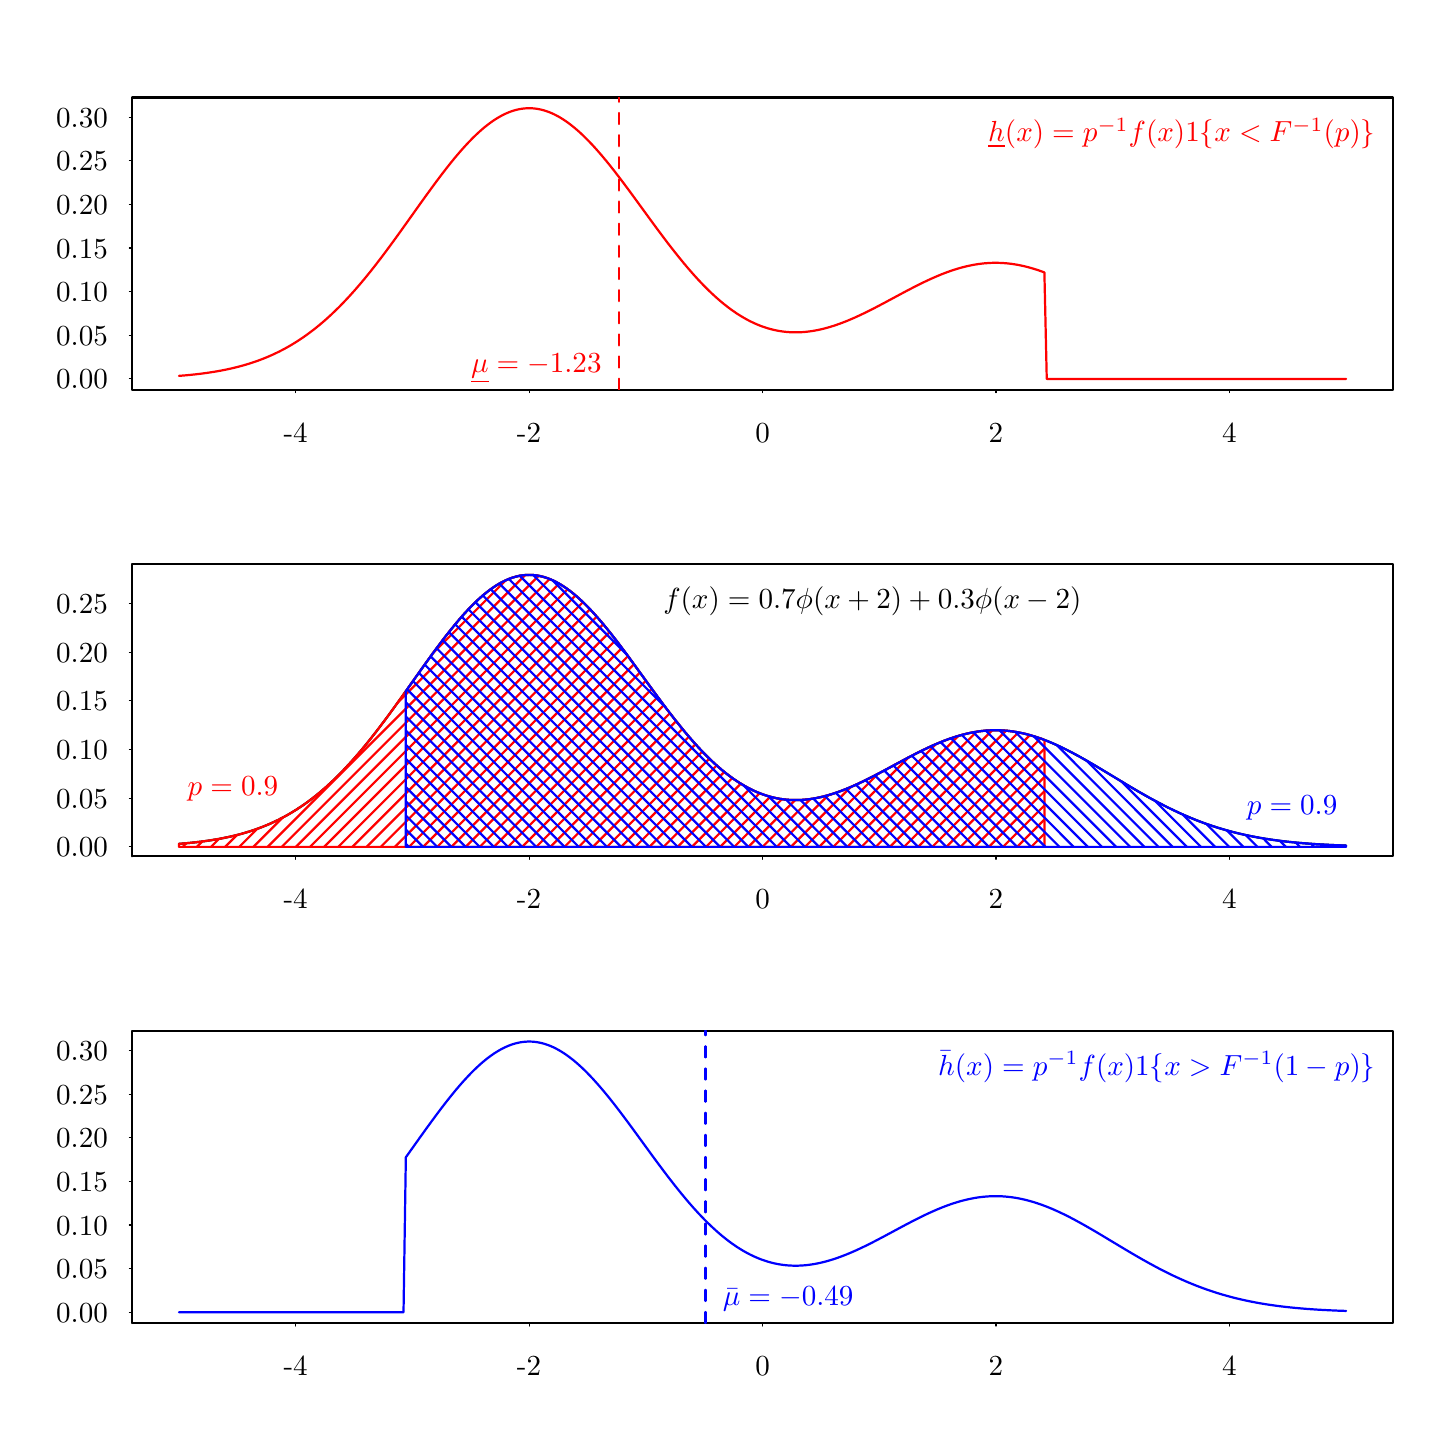
\begin{tikzpicture}[x=1pt,y=1pt]
\definecolor{fillColor}{RGB}{255,255,255}
\path[use as bounding box,fill=fillColor,fill opacity=0.00] (0,0) rectangle (505.89,505.89);
\begin{scope}
\path[clip] ( 37.80,375.06) rectangle (493.29,480.69);
\definecolor{drawColor}{RGB}{255,0,0}

\path[draw=drawColor,line width= 0.8pt,line join=round,line cap=round] ( 54.67,380.06) --
	( 55.52,380.13) --
	( 56.36,380.20) --
	( 57.21,380.27) --
	( 58.05,380.35) --
	( 58.90,380.43) --
	( 59.74,380.52) --
	( 60.59,380.61) --
	( 61.43,380.71) --
	( 62.28,380.81) --
	( 63.12,380.91) --
	( 63.97,381.03) --
	( 64.81,381.14) --
	( 65.66,381.27) --
	( 66.50,381.40) --
	( 67.35,381.53) --
	( 68.19,381.67) --
	( 69.04,381.82) --
	( 69.88,381.98) --
	( 70.73,382.14) --
	( 71.57,382.31) --
	( 72.42,382.49) --
	( 73.26,382.67) --
	( 74.11,382.87) --
	( 74.95,383.07) --
	( 75.80,383.28) --
	( 76.64,383.50) --
	( 77.49,383.73) --
	( 78.34,383.97) --
	( 79.18,384.22) --
	( 80.03,384.48) --
	( 80.87,384.75) --
	( 81.72,385.03) --
	( 82.56,385.32) --
	( 83.41,385.62) --
	( 84.25,385.94) --
	( 85.10,386.27) --
	( 85.94,386.60) --
	( 86.79,386.96) --
	( 87.63,387.32) --
	( 88.48,387.70) --
	( 89.32,388.09) --
	( 90.17,388.50) --
	( 91.01,388.91) --
	( 91.86,389.35) --
	( 92.70,389.79) --
	( 93.55,390.26) --
	( 94.39,390.73) --
	( 95.24,391.23) --
	( 96.08,391.74) --
	( 96.93,392.26) --
	( 97.77,392.80) --
	( 98.62,393.36) --
	( 99.47,393.93) --
	(100.31,394.52) --
	(101.16,395.12) --
	(102.00,395.75) --
	(102.85,396.39) --
	(103.69,397.04) --
	(104.54,397.72) --
	(105.38,398.41) --
	(106.23,399.12) --
	(107.07,399.84) --
	(107.92,400.59) --
	(108.76,401.35) --
	(109.61,402.13) --
	(110.45,402.93) --
	(111.30,403.74) --
	(112.14,404.57) --
	(112.99,405.42) --
	(113.83,406.28) --
	(114.68,407.17) --
	(115.52,408.07) --
	(116.37,408.98) --
	(117.21,409.92) --
	(118.06,410.86) --
	(118.90,411.83) --
	(119.75,412.81) --
	(120.59,413.80) --
	(121.44,414.82) --
	(122.29,415.84) --
	(123.13,416.88) --
	(123.98,417.93) --
	(124.82,419.00) --
	(125.67,420.08) --
	(126.51,421.17) --
	(127.36,422.27) --
	(128.20,423.38) --
	(129.05,424.50) --
	(129.89,425.64) --
	(130.74,426.78) --
	(131.58,427.93) --
	(132.43,429.09) --
	(133.27,430.25) --
	(134.12,431.42) --
	(134.96,432.60) --
	(135.81,433.78) --
	(136.65,434.96) --
	(137.50,436.15) --
	(138.34,437.34) --
	(139.19,438.52) --
	(140.03,439.71) --
	(140.88,440.90) --
	(141.72,442.09) --
	(142.57,443.27) --
	(143.41,444.45) --
	(144.26,445.62) --
	(145.11,446.78) --
	(145.95,447.94) --
	(146.80,449.09) --
	(147.64,450.24) --
	(148.49,451.37) --
	(149.33,452.49) --
	(150.18,453.59) --
	(151.02,454.68) --
	(151.87,455.76) --
	(152.71,456.82) --
	(153.56,457.87) --
	(154.40,458.90) --
	(155.25,459.90) --
	(156.09,460.89) --
	(156.94,461.86) --
	(157.78,462.80) --
	(158.63,463.72) --
	(159.47,464.62) --
	(160.32,465.49) --
	(161.16,466.34) --
	(162.01,467.15) --
	(162.85,467.94) --
	(163.70,468.71) --
	(164.54,469.44) --
	(165.39,470.14) --
	(166.24,470.81) --
	(167.08,471.44) --
	(167.93,472.05) --
	(168.77,472.62) --
	(169.62,473.15) --
	(170.46,473.65) --
	(171.31,474.12) --
	(172.15,474.55) --
	(173.00,474.94) --
	(173.84,475.30) --
	(174.69,475.62) --
	(175.53,475.90) --
	(176.38,476.14) --
	(177.22,476.34) --
	(178.07,476.51) --
	(178.91,476.63) --
	(179.76,476.72) --
	(180.60,476.77) --
	(181.45,476.78) --
	(182.29,476.75) --
	(183.14,476.68) --
	(183.98,476.57) --
	(184.83,476.42) --
	(185.67,476.24) --
	(186.52,476.01) --
	(187.36,475.75) --
	(188.21,475.45) --
	(189.06,475.11) --
	(189.90,474.74) --
	(190.75,474.32) --
	(191.59,473.88) --
	(192.44,473.39) --
	(193.28,472.87) --
	(194.13,472.32) --
	(194.97,471.73) --
	(195.82,471.11) --
	(196.66,470.46) --
	(197.51,469.78) --
	(198.35,469.06) --
	(199.20,468.32) --
	(200.04,467.55) --
	(200.89,466.75) --
	(201.73,465.92) --
	(202.58,465.06) --
	(203.42,464.18) --
	(204.27,463.28) --
	(205.11,462.35) --
	(205.96,461.40) --
	(206.80,460.43) --
	(207.65,459.44) --
	(208.49,458.43) --
	(209.34,457.41) --
	(210.19,456.36) --
	(211.03,455.30) --
	(211.88,454.23) --
	(212.72,453.14) --
	(213.57,452.04) --
	(214.41,450.93) --
	(215.26,449.81) --
	(216.10,448.68) --
	(216.95,447.54) --
	(217.79,446.40) --
	(218.64,445.24) --
	(219.48,444.09) --
	(220.33,442.93) --
	(221.17,441.77) --
	(222.02,440.61) --
	(222.86,439.45) --
	(223.71,438.29) --
	(224.55,437.13) --
	(225.40,435.97) --
	(226.24,434.82) --
	(227.09,433.67) --
	(227.93,432.53) --
	(228.78,431.40) --
	(229.62,430.27) --
	(230.47,429.15) --
	(231.31,428.04) --
	(232.16,426.94) --
	(233.01,425.86) --
	(233.85,424.78) --
	(234.70,423.72) --
	(235.54,422.67) --
	(236.39,421.63) --
	(237.23,420.61) --
	(238.08,419.60) --
	(238.92,418.61) --
	(239.77,417.64) --
	(240.61,416.68) --
	(241.46,415.74) --
	(242.30,414.82) --
	(243.15,413.92) --
	(243.99,413.04) --
	(244.84,412.18) --
	(245.68,411.33) --
	(246.53,410.51) --
	(247.37,409.71) --
	(248.22,408.93) --
	(249.06,408.17) --
	(249.91,407.43) --
	(250.75,406.71) --
	(251.60,406.02) --
	(252.44,405.35) --
	(253.29,404.70) --
	(254.13,404.07) --
	(254.98,403.47) --
	(255.83,402.89) --
	(256.67,402.33) --
	(257.52,401.80) --
	(258.36,401.29) --
	(259.21,400.80) --
	(260.05,400.33) --
	(260.90,399.89) --
	(261.74,399.48) --
	(262.59,399.08) --
	(263.43,398.71) --
	(264.28,398.36) --
	(265.12,398.03) --
	(265.97,397.73) --
	(266.81,397.45) --
	(267.66,397.19) --
	(268.50,396.96) --
	(269.35,396.74) --
	(270.19,396.55) --
	(271.04,396.38) --
	(271.88,396.24) --
	(272.73,396.11) --
	(273.57,396.01) --
	(274.42,395.92) --
	(275.26,395.86) --
	(276.11,395.82) --
	(276.96,395.79) --
	(277.80,395.79) --
	(278.65,395.81) --
	(279.49,395.84) --
	(280.34,395.90) --
	(281.18,395.97) --
	(282.03,396.07) --
	(282.87,396.18) --
	(283.72,396.30) --
	(284.56,396.45) --
	(285.41,396.61) --
	(286.25,396.79) --
	(287.10,396.98) --
	(287.94,397.19) --
	(288.79,397.42) --
	(289.63,397.66) --
	(290.48,397.92) --
	(291.32,398.18) --
	(292.17,398.47) --
	(293.01,398.76) --
	(293.86,399.07) --
	(294.70,399.39) --
	(295.55,399.72) --
	(296.39,400.06) --
	(297.24,400.42) --
	(298.08,400.78) --
	(298.93,401.15) --
	(299.78,401.54) --
	(300.62,401.93) --
	(301.47,402.33) --
	(302.31,402.73) --
	(303.16,403.15) --
	(304.00,403.57) --
	(304.85,403.99) --
	(305.69,404.42) --
	(306.54,404.86) --
	(307.38,405.30) --
	(308.23,405.75) --
	(309.07,406.19) --
	(309.92,406.64) --
	(310.76,407.10) --
	(311.61,407.55) --
	(312.45,408.00) --
	(313.30,408.46) --
	(314.14,408.91) --
	(314.99,409.37) --
	(315.83,409.82) --
	(316.68,410.27) --
	(317.52,410.72) --
	(318.37,411.16) --
	(319.21,411.60) --
	(320.06,412.04) --
	(320.90,412.47) --
	(321.75,412.90) --
	(322.60,413.32) --
	(323.44,413.73) --
	(324.29,414.14) --
	(325.13,414.54) --
	(325.98,414.93) --
	(326.82,415.31) --
	(327.67,415.68) --
	(328.51,416.05) --
	(329.36,416.40) --
	(330.20,416.75) --
	(331.05,417.08) --
	(331.89,417.40) --
	(332.74,417.71) --
	(333.58,418.01) --
	(334.43,418.29) --
	(335.27,418.56) --
	(336.12,418.82) --
	(336.96,419.07) --
	(337.81,419.30) --
	(338.65,419.51) --
	(339.50,419.71) --
	(340.34,419.90) --
	(341.19,420.07) --
	(342.03,420.23) --
	(342.88,420.37) --
	(343.73,420.50) --
	(344.57,420.60) --
	(345.42,420.70) --
	(346.26,420.77) --
	(347.11,420.83) --
	(347.95,420.88) --
	(348.80,420.91) --
	(349.64,420.92) --
	(350.49,420.91) --
	(351.33,420.89) --
	(352.18,420.85) --
	(353.02,420.79) --
	(353.87,420.72) --
	(354.71,420.63) --
	(355.56,420.53) --
	(356.40,420.40) --
	(357.25,420.27) --
	(358.09,420.11) --
	(358.94,419.94) --
	(359.78,419.76) --
	(360.63,419.56) --
	(361.47,419.34) --
	(362.32,419.11) --
	(363.16,418.87) --
	(364.01,418.61) --
	(364.85,418.34) --
	(365.70,418.05) --
	(366.55,417.75) --
	(367.39,417.43) --
	(368.24,378.97) --
	(369.08,378.97) --
	(369.93,378.97) --
	(370.77,378.97) --
	(371.62,378.97) --
	(372.46,378.97) --
	(373.31,378.97) --
	(374.15,378.97) --
	(375.00,378.97) --
	(375.84,378.97) --
	(376.69,378.97) --
	(377.53,378.97) --
	(378.38,378.97) --
	(379.22,378.97) --
	(380.07,378.97) --
	(380.91,378.97) --
	(381.76,378.97) --
	(382.60,378.97) --
	(383.45,378.97) --
	(384.29,378.97) --
	(385.14,378.97) --
	(385.98,378.97) --
	(386.83,378.97) --
	(387.68,378.97) --
	(388.52,378.97) --
	(389.37,378.97) --
	(390.21,378.97) --
	(391.06,378.97) --
	(391.90,378.97) --
	(392.75,378.97) --
	(393.59,378.97) --
	(394.44,378.97) --
	(395.28,378.97) --
	(396.13,378.97) --
	(396.97,378.97) --
	(397.82,378.97) --
	(398.66,378.97) --
	(399.51,378.97) --
	(400.35,378.97) --
	(401.20,378.97) --
	(402.04,378.97) --
	(402.89,378.97) --
	(403.73,378.97) --
	(404.58,378.97) --
	(405.42,378.97) --
	(406.27,378.97) --
	(407.11,378.97) --
	(407.96,378.97) --
	(408.80,378.97) --
	(409.65,378.97) --
	(410.50,378.97) --
	(411.34,378.97) --
	(412.19,378.97) --
	(413.03,378.97) --
	(413.88,378.97) --
	(414.72,378.97) --
	(415.57,378.97) --
	(416.41,378.97) --
	(417.26,378.97) --
	(418.10,378.97) --
	(418.95,378.97) --
	(419.79,378.97) --
	(420.64,378.97) --
	(421.48,378.97) --
	(422.33,378.97) --
	(423.17,378.97) --
	(424.02,378.97) --
	(424.86,378.97) --
	(425.71,378.97) --
	(426.55,378.97) --
	(427.40,378.97) --
	(428.24,378.97) --
	(429.09,378.97) --
	(429.93,378.97) --
	(430.78,378.97) --
	(431.62,378.97) --
	(432.47,378.97) --
	(433.32,378.97) --
	(434.16,378.97) --
	(435.01,378.97) --
	(435.85,378.97) --
	(436.70,378.97) --
	(437.54,378.97) --
	(438.39,378.97) --
	(439.23,378.97) --
	(440.08,378.97) --
	(440.92,378.97) --
	(441.77,378.97) --
	(442.61,378.97) --
	(443.46,378.97) --
	(444.30,378.97) --
	(445.15,378.97) --
	(445.99,378.97) --
	(446.84,378.97) --
	(447.68,378.97) --
	(448.53,378.97) --
	(449.37,378.97) --
	(450.22,378.97) --
	(451.06,378.97) --
	(451.91,378.97) --
	(452.75,378.97) --
	(453.60,378.97) --
	(454.45,378.97) --
	(455.29,378.97) --
	(456.14,378.97) --
	(456.98,378.97) --
	(457.83,378.97) --
	(458.67,378.97) --
	(459.52,378.97) --
	(460.36,378.97) --
	(461.21,378.97) --
	(462.05,378.97) --
	(462.90,378.97) --
	(463.74,378.97) --
	(464.59,378.97) --
	(465.43,378.97) --
	(466.28,378.97) --
	(467.12,378.97) --
	(467.97,378.97) --
	(468.81,378.97) --
	(469.66,378.97) --
	(470.50,378.97) --
	(471.35,378.97) --
	(472.19,378.97) --
	(473.04,378.97) --
	(473.88,378.97) --
	(474.73,378.97) --
	(475.57,378.97) --
	(476.42,378.97);
\end{scope}
\begin{scope}
\path[clip] (  0.00,  0.00) rectangle (505.89,505.89);
\definecolor{drawColor}{RGB}{0,0,0}

\path[draw=drawColor,line width= 0.4pt,line join=round,line cap=round] ( 96.84,375.06) -- (434.25,375.06);

\path[draw=drawColor,line width= 0.4pt,line join=round,line cap=round] ( 96.84,375.06) -- ( 96.84,374.00);

\path[draw=drawColor,line width= 0.4pt,line join=round,line cap=round] (181.19,375.06) -- (181.19,374.00);

\path[draw=drawColor,line width= 0.4pt,line join=round,line cap=round] (265.54,375.06) -- (265.54,374.00);

\path[draw=drawColor,line width= 0.4pt,line join=round,line cap=round] (349.89,375.06) -- (349.89,374.00);

\path[draw=drawColor,line width= 0.4pt,line join=round,line cap=round] (434.25,375.06) -- (434.25,374.00);

\node[text=drawColor,anchor=base,inner sep=0pt, outer sep=0pt, scale=  1.05] at ( 96.84,356.16) {-4};

\node[text=drawColor,anchor=base,inner sep=0pt, outer sep=0pt, scale=  1.05] at (181.19,356.16) {-2};

\node[text=drawColor,anchor=base,inner sep=0pt, outer sep=0pt, scale=  1.05] at (265.54,356.16) {0};

\node[text=drawColor,anchor=base,inner sep=0pt, outer sep=0pt, scale=  1.05] at (349.89,356.16) {2};

\node[text=drawColor,anchor=base,inner sep=0pt, outer sep=0pt, scale=  1.05] at (434.25,356.16) {4};

\path[draw=drawColor,line width= 0.4pt,line join=round,line cap=round] ( 37.80,378.97) -- ( 37.80,473.52);

\path[draw=drawColor,line width= 0.4pt,line join=round,line cap=round] ( 37.80,378.97) -- ( 36.74,378.97);

\path[draw=drawColor,line width= 0.4pt,line join=round,line cap=round] ( 37.80,394.73) -- ( 36.74,394.73);

\path[draw=drawColor,line width= 0.4pt,line join=round,line cap=round] ( 37.80,410.49) -- ( 36.74,410.49);

\path[draw=drawColor,line width= 0.4pt,line join=round,line cap=round] ( 37.80,426.25) -- ( 36.74,426.25);

\path[draw=drawColor,line width= 0.4pt,line join=round,line cap=round] ( 37.80,442.01) -- ( 36.74,442.01);

\path[draw=drawColor,line width= 0.4pt,line join=round,line cap=round] ( 37.80,457.76) -- ( 36.74,457.76);

\path[draw=drawColor,line width= 0.4pt,line join=round,line cap=round] ( 37.80,473.52) -- ( 36.74,473.52);

\node[text=drawColor,anchor=base east,inner sep=0pt, outer sep=0pt, scale=  1.05] at ( 28.98,375.36) {0.00};

\node[text=drawColor,anchor=base east,inner sep=0pt, outer sep=0pt, scale=  1.05] at ( 28.98,391.11) {0.05};

\node[text=drawColor,anchor=base east,inner sep=0pt, outer sep=0pt, scale=  1.05] at ( 28.98,406.87) {0.10};

\node[text=drawColor,anchor=base east,inner sep=0pt, outer sep=0pt, scale=  1.05] at ( 28.98,422.63) {0.15};

\node[text=drawColor,anchor=base east,inner sep=0pt, outer sep=0pt, scale=  1.05] at ( 28.98,438.39) {0.20};

\node[text=drawColor,anchor=base east,inner sep=0pt, outer sep=0pt, scale=  1.05] at ( 28.98,454.15) {0.25};

\node[text=drawColor,anchor=base east,inner sep=0pt, outer sep=0pt, scale=  1.05] at ( 28.98,469.91) {0.30};

\path[draw=drawColor,line width= 0.8pt,line join=round,line cap=round] ( 37.80,375.06) --
	(493.29,375.06) --
	(493.29,480.69) --
	( 37.80,480.69) --
	( 37.80,375.06);
\end{scope}
\begin{scope}
\path[clip] ( 37.80,375.06) rectangle (493.29,480.69);
\definecolor{drawColor}{RGB}{255,0,0}

\node[text=drawColor,anchor=base east,inner sep=0pt, outer sep=0pt, scale=  1.05] at (486.99,464.59) {$\underline{h}(x) = p^{-1}f(x) 1\{x < F^{-1}(p)\}$};

\path[draw=drawColor,line width= 0.8pt,dash pattern=on 4pt off 4pt ,line join=round,line cap=round] (213.67,375.06) -- (213.67,480.69);

\node[text=drawColor,anchor=base east,inner sep=0pt, outer sep=0pt, scale=  1.05] at (207.37,381.45) {$\underline{\mu} = -1.23$};
\end{scope}
\begin{scope}
\path[clip] ( 37.80,206.43) rectangle (493.29,312.06);
\definecolor{drawColor}{RGB}{0,0,0}

\path[draw=drawColor,line width= 0.8pt,line join=round,line cap=round] ( 54.67,210.97) --
	( 55.52,211.03) --
	( 56.36,211.10) --
	( 57.21,211.18) --
	( 58.05,211.26) --
	( 58.90,211.34) --
	( 59.74,211.43) --
	( 60.59,211.52) --
	( 61.43,211.62) --
	( 62.28,211.72) --
	( 63.12,211.83) --
	( 63.97,211.94) --
	( 64.81,212.06) --
	( 65.66,212.18) --
	( 66.50,212.31) --
	( 67.35,212.45) --
	( 68.19,212.59) --
	( 69.04,212.74) --
	( 69.88,212.89) --
	( 70.73,213.06) --
	( 71.57,213.23) --
	( 72.42,213.41) --
	( 73.26,213.59) --
	( 74.11,213.79) --
	( 74.95,213.99) --
	( 75.80,214.20) --
	( 76.64,214.42) --
	( 77.49,214.65) --
	( 78.34,214.90) --
	( 79.18,215.15) --
	( 80.03,215.41) --
	( 80.87,215.68) --
	( 81.72,215.96) --
	( 82.56,216.25) --
	( 83.41,216.56) --
	( 84.25,216.87) --
	( 85.10,217.20) --
	( 85.94,217.54) --
	( 86.79,217.90) --
	( 87.63,218.26) --
	( 88.48,218.64) --
	( 89.32,219.04) --
	( 90.17,219.44) --
	( 91.01,219.86) --
	( 91.86,220.30) --
	( 92.70,220.75) --
	( 93.55,221.21) --
	( 94.39,221.69) --
	( 95.24,222.19) --
	( 96.08,222.70) --
	( 96.93,223.23) --
	( 97.77,223.77) --
	( 98.62,224.33) --
	( 99.47,224.90) --
	(100.31,225.49) --
	(101.16,226.10) --
	(102.00,226.73) --
	(102.85,227.37) --
	(103.69,228.03) --
	(104.54,228.71) --
	(105.38,229.40) --
	(106.23,230.12) --
	(107.07,230.85) --
	(107.92,231.59) --
	(108.76,232.36) --
	(109.61,233.14) --
	(110.45,233.94) --
	(111.30,234.76) --
	(112.14,235.59) --
	(112.99,236.45) --
	(113.83,237.32) --
	(114.68,238.20) --
	(115.52,239.11) --
	(116.37,240.03) --
	(117.21,240.97) --
	(118.06,241.92) --
	(118.90,242.89) --
	(119.75,243.87) --
	(120.59,244.87) --
	(121.44,245.89) --
	(122.29,246.92) --
	(123.13,247.96) --
	(123.98,249.02) --
	(124.82,250.09) --
	(125.67,251.17) --
	(126.51,252.27) --
	(127.36,253.38) --
	(128.20,254.50) --
	(129.05,255.62) --
	(129.89,256.76) --
	(130.74,257.91) --
	(131.58,259.07) --
	(132.43,260.23) --
	(133.27,261.40) --
	(134.12,262.58) --
	(134.96,263.76) --
	(135.81,264.94) --
	(136.65,266.13) --
	(137.50,267.32) --
	(138.34,268.52) --
	(139.19,269.71) --
	(140.03,270.91) --
	(140.88,272.10) --
	(141.72,273.29) --
	(142.57,274.48) --
	(143.41,275.66) --
	(144.26,276.84) --
	(145.11,278.01) --
	(145.95,279.18) --
	(146.80,280.33) --
	(147.64,281.48) --
	(148.49,282.61) --
	(149.33,283.74) --
	(150.18,284.85) --
	(151.02,285.95) --
	(151.87,287.03) --
	(152.71,288.10) --
	(153.56,289.15) --
	(154.40,290.18) --
	(155.25,291.19) --
	(156.09,292.19) --
	(156.94,293.16) --
	(157.78,294.11) --
	(158.63,295.03) --
	(159.47,295.93) --
	(160.32,296.81) --
	(161.16,297.66) --
	(162.01,298.48) --
	(162.85,299.27) --
	(163.70,300.04) --
	(164.54,300.77) --
	(165.39,301.47) --
	(166.24,302.15) --
	(167.08,302.79) --
	(167.93,303.39) --
	(168.77,303.97) --
	(169.62,304.51) --
	(170.46,305.01) --
	(171.31,305.48) --
	(172.15,305.91) --
	(173.00,306.30) --
	(173.84,306.66) --
	(174.69,306.98) --
	(175.53,307.26) --
	(176.38,307.50) --
	(177.22,307.71) --
	(178.07,307.88) --
	(178.91,308.00) --
	(179.76,308.09) --
	(180.60,308.14) --
	(181.45,308.15) --
	(182.29,308.12) --
	(183.14,308.05) --
	(183.98,307.94) --
	(184.83,307.79) --
	(185.67,307.60) --
	(186.52,307.38) --
	(187.36,307.11) --
	(188.21,306.81) --
	(189.06,306.47) --
	(189.90,306.10) --
	(190.75,305.68) --
	(191.59,305.23) --
	(192.44,304.75) --
	(193.28,304.22) --
	(194.13,303.67) --
	(194.97,303.08) --
	(195.82,302.46) --
	(196.66,301.80) --
	(197.51,301.12) --
	(198.35,300.40) --
	(199.20,299.65) --
	(200.04,298.87) --
	(200.89,298.07) --
	(201.73,297.24) --
	(202.58,296.38) --
	(203.42,295.49) --
	(204.27,294.59) --
	(205.11,293.65) --
	(205.96,292.70) --
	(206.80,291.73) --
	(207.65,290.73) --
	(208.49,289.72) --
	(209.34,288.68) --
	(210.19,287.63) --
	(211.03,286.57) --
	(211.88,285.49) --
	(212.72,284.40) --
	(213.57,283.29) --
	(214.41,282.18) --
	(215.26,281.05) --
	(216.10,279.91) --
	(216.95,278.77) --
	(217.79,277.62) --
	(218.64,276.46) --
	(219.48,275.30) --
	(220.33,274.14) --
	(221.17,272.97) --
	(222.02,271.81) --
	(222.86,270.64) --
	(223.71,269.47) --
	(224.55,268.31) --
	(225.40,267.15) --
	(226.24,265.99) --
	(227.09,264.84) --
	(227.93,263.69) --
	(228.78,262.55) --
	(229.62,261.42) --
	(230.47,260.29) --
	(231.31,259.18) --
	(232.16,258.08) --
	(233.01,256.98) --
	(233.85,255.90) --
	(234.70,254.83) --
	(235.54,253.78) --
	(236.39,252.74) --
	(237.23,251.71) --
	(238.08,250.70) --
	(238.92,249.71) --
	(239.77,248.73) --
	(240.61,247.77) --
	(241.46,246.82) --
	(242.30,245.90) --
	(243.15,244.99) --
	(243.99,244.10) --
	(244.84,243.24) --
	(245.68,242.39) --
	(246.53,241.56) --
	(247.37,240.76) --
	(248.22,239.97) --
	(249.06,239.21) --
	(249.91,238.47) --
	(250.75,237.75) --
	(251.60,237.05) --
	(252.44,236.38) --
	(253.29,235.73) --
	(254.13,235.10) --
	(254.98,234.49) --
	(255.83,233.91) --
	(256.67,233.35) --
	(257.52,232.81) --
	(258.36,232.30) --
	(259.21,231.81) --
	(260.05,231.34) --
	(260.90,230.90) --
	(261.74,230.48) --
	(262.59,230.08) --
	(263.43,229.70) --
	(264.28,229.35) --
	(265.12,229.03) --
	(265.97,228.72) --
	(266.81,228.44) --
	(267.66,228.18) --
	(268.50,227.94) --
	(269.35,227.73) --
	(270.19,227.54) --
	(271.04,227.37) --
	(271.88,227.22) --
	(272.73,227.09) --
	(273.57,226.99) --
	(274.42,226.90) --
	(275.26,226.84) --
	(276.11,226.80) --
	(276.96,226.78) --
	(277.80,226.77) --
	(278.65,226.79) --
	(279.49,226.83) --
	(280.34,226.88) --
	(281.18,226.96) --
	(282.03,227.05) --
	(282.87,227.16) --
	(283.72,227.29) --
	(284.56,227.44) --
	(285.41,227.60) --
	(286.25,227.78) --
	(287.10,227.97) --
	(287.94,228.18) --
	(288.79,228.41) --
	(289.63,228.65) --
	(290.48,228.91) --
	(291.32,229.18) --
	(292.17,229.46) --
	(293.01,229.76) --
	(293.86,230.07) --
	(294.70,230.39) --
	(295.55,230.72) --
	(296.39,231.07) --
	(297.24,231.42) --
	(298.08,231.79) --
	(298.93,232.16) --
	(299.78,232.55) --
	(300.62,232.94) --
	(301.47,233.34) --
	(302.31,233.75) --
	(303.16,234.16) --
	(304.00,234.59) --
	(304.85,235.01) --
	(305.69,235.45) --
	(306.54,235.89) --
	(307.38,236.33) --
	(308.23,236.78) --
	(309.07,237.23) --
	(309.92,237.68) --
	(310.76,238.13) --
	(311.61,238.59) --
	(312.45,239.05) --
	(313.30,239.50) --
	(314.14,239.96) --
	(314.99,240.41) --
	(315.83,240.87) --
	(316.68,241.32) --
	(317.52,241.77) --
	(318.37,242.22) --
	(319.21,242.66) --
	(320.06,243.10) --
	(320.90,243.53) --
	(321.75,243.96) --
	(322.60,244.38) --
	(323.44,244.80) --
	(324.29,245.21) --
	(325.13,245.61) --
	(325.98,246.00) --
	(326.82,246.39) --
	(327.67,246.76) --
	(328.51,247.13) --
	(329.36,247.48) --
	(330.20,247.83) --
	(331.05,248.16) --
	(331.89,248.49) --
	(332.74,248.80) --
	(333.58,249.09) --
	(334.43,249.38) --
	(335.27,249.65) --
	(336.12,249.91) --
	(336.96,250.16) --
	(337.81,250.39) --
	(338.65,250.61) --
	(339.50,250.81) --
	(340.34,251.00) --
	(341.19,251.17) --
	(342.03,251.33) --
	(342.88,251.47) --
	(343.73,251.60) --
	(344.57,251.71) --
	(345.42,251.80) --
	(346.26,251.88) --
	(347.11,251.94) --
	(347.95,251.98) --
	(348.80,252.01) --
	(349.64,252.02) --
	(350.49,252.01) --
	(351.33,251.99) --
	(352.18,251.95) --
	(353.02,251.89) --
	(353.87,251.82) --
	(354.71,251.73) --
	(355.56,251.63) --
	(356.40,251.51) --
	(357.25,251.37) --
	(358.09,251.21) --
	(358.94,251.04) --
	(359.78,250.86) --
	(360.63,250.66) --
	(361.47,250.44) --
	(362.32,250.21) --
	(363.16,249.96) --
	(364.01,249.70) --
	(364.85,249.43) --
	(365.70,249.14) --
	(366.55,248.84) --
	(367.39,248.52) --
	(368.24,248.19) --
	(369.08,247.85) --
	(369.93,247.50) --
	(370.77,247.13) --
	(371.62,246.76) --
	(372.46,246.37) --
	(373.31,245.98) --
	(374.15,245.57) --
	(375.00,245.15) --
	(375.84,244.73) --
	(376.69,244.29) --
	(377.53,243.85) --
	(378.38,243.40) --
	(379.22,242.94) --
	(380.07,242.48) --
	(380.91,242.01) --
	(381.76,241.53) --
	(382.60,241.05) --
	(383.45,240.56) --
	(384.29,240.07) --
	(385.14,239.58) --
	(385.98,239.08) --
	(386.83,238.57) --
	(387.68,238.07) --
	(388.52,237.56) --
	(389.37,237.05) --
	(390.21,236.54) --
	(391.06,236.03) --
	(391.90,235.52) --
	(392.75,235.01) --
	(393.59,234.50) --
	(394.44,233.98) --
	(395.28,233.48) --
	(396.13,232.97) --
	(396.97,232.46) --
	(397.82,231.96) --
	(398.66,231.46) --
	(399.51,230.96) --
	(400.35,230.46) --
	(401.20,229.97) --
	(402.04,229.48) --
	(402.89,229.00) --
	(403.73,228.52) --
	(404.58,228.04) --
	(405.42,227.57) --
	(406.27,227.11) --
	(407.11,226.65) --
	(407.96,226.20) --
	(408.80,225.75) --
	(409.65,225.31) --
	(410.50,224.87) --
	(411.34,224.45) --
	(412.19,224.02) --
	(413.03,223.61) --
	(413.88,223.20) --
	(414.72,222.80) --
	(415.57,222.40) --
	(416.41,222.02) --
	(417.26,221.64) --
	(418.10,221.26) --
	(418.95,220.90) --
	(419.79,220.54) --
	(420.64,220.19) --
	(421.48,219.85) --
	(422.33,219.51) --
	(423.17,219.18) --
	(424.02,218.86) --
	(424.86,218.55) --
	(425.71,218.24) --
	(426.55,217.95) --
	(427.40,217.66) --
	(428.24,217.37) --
	(429.09,217.10) --
	(429.93,216.83) --
	(430.78,216.57) --
	(431.62,216.32) --
	(432.47,216.07) --
	(433.32,215.83) --
	(434.16,215.60) --
	(435.01,215.37) --
	(435.85,215.15) --
	(436.70,214.94) --
	(437.54,214.73) --
	(438.39,214.53) --
	(439.23,214.34) --
	(440.08,214.16) --
	(440.92,213.98) --
	(441.77,213.80) --
	(442.61,213.63) --
	(443.46,213.47) --
	(444.30,213.31) --
	(445.15,213.16) --
	(445.99,213.02) --
	(446.84,212.87) --
	(447.68,212.74) --
	(448.53,212.61) --
	(449.37,212.48) --
	(450.22,212.36) --
	(451.06,212.25) --
	(451.91,212.13) --
	(452.75,212.03) --
	(453.60,211.92) --
	(454.45,211.82) --
	(455.29,211.73) --
	(456.14,211.64) --
	(456.98,211.55) --
	(457.83,211.47) --
	(458.67,211.39) --
	(459.52,211.31) --
	(460.36,211.24) --
	(461.21,211.17) --
	(462.05,211.10) --
	(462.90,211.04) --
	(463.74,210.98) --
	(464.59,210.92) --
	(465.43,210.86) --
	(466.28,210.81) --
	(467.12,210.76) --
	(467.97,210.71) --
	(468.81,210.67) --
	(469.66,210.62) --
	(470.50,210.58) --
	(471.35,210.54) --
	(472.19,210.50) --
	(473.04,210.47) --
	(473.88,210.43) --
	(474.73,210.40) --
	(475.57,210.37) --
	(476.42,210.34);
\end{scope}
\begin{scope}
\path[clip] (  0.00,  0.00) rectangle (505.89,505.89);
\definecolor{drawColor}{RGB}{0,0,0}

\path[draw=drawColor,line width= 0.4pt,line join=round,line cap=round] ( 96.84,206.43) -- (434.25,206.43);

\path[draw=drawColor,line width= 0.4pt,line join=round,line cap=round] ( 96.84,206.43) -- ( 96.84,205.37);

\path[draw=drawColor,line width= 0.4pt,line join=round,line cap=round] (181.19,206.43) -- (181.19,205.37);

\path[draw=drawColor,line width= 0.4pt,line join=round,line cap=round] (265.54,206.43) -- (265.54,205.37);

\path[draw=drawColor,line width= 0.4pt,line join=round,line cap=round] (349.89,206.43) -- (349.89,205.37);

\path[draw=drawColor,line width= 0.4pt,line join=round,line cap=round] (434.25,206.43) -- (434.25,205.37);

\node[text=drawColor,anchor=base,inner sep=0pt, outer sep=0pt, scale=  1.05] at ( 96.84,187.53) {-4};

\node[text=drawColor,anchor=base,inner sep=0pt, outer sep=0pt, scale=  1.05] at (181.19,187.53) {-2};

\node[text=drawColor,anchor=base,inner sep=0pt, outer sep=0pt, scale=  1.05] at (265.54,187.53) {0};

\node[text=drawColor,anchor=base,inner sep=0pt, outer sep=0pt, scale=  1.05] at (349.89,187.53) {2};

\node[text=drawColor,anchor=base,inner sep=0pt, outer sep=0pt, scale=  1.05] at (434.25,187.53) {4};

\path[draw=drawColor,line width= 0.4pt,line join=round,line cap=round] ( 37.80,209.87) -- ( 37.80,297.84);

\path[draw=drawColor,line width= 0.4pt,line join=round,line cap=round] ( 37.80,209.87) -- ( 36.74,209.87);

\path[draw=drawColor,line width= 0.4pt,line join=round,line cap=round] ( 37.80,227.47) -- ( 36.74,227.47);

\path[draw=drawColor,line width= 0.4pt,line join=round,line cap=round] ( 37.80,245.06) -- ( 36.74,245.06);

\path[draw=drawColor,line width= 0.4pt,line join=round,line cap=round] ( 37.80,262.65) -- ( 36.74,262.65);

\path[draw=drawColor,line width= 0.4pt,line join=round,line cap=round] ( 37.80,280.25) -- ( 36.74,280.25);

\path[draw=drawColor,line width= 0.4pt,line join=round,line cap=round] ( 37.80,297.84) -- ( 36.74,297.84);

\node[text=drawColor,anchor=base east,inner sep=0pt, outer sep=0pt, scale=  1.05] at ( 28.98,206.26) {0.00};

\node[text=drawColor,anchor=base east,inner sep=0pt, outer sep=0pt, scale=  1.05] at ( 28.98,223.85) {0.05};

\node[text=drawColor,anchor=base east,inner sep=0pt, outer sep=0pt, scale=  1.05] at ( 28.98,241.44) {0.10};

\node[text=drawColor,anchor=base east,inner sep=0pt, outer sep=0pt, scale=  1.05] at ( 28.98,259.04) {0.15};

\node[text=drawColor,anchor=base east,inner sep=0pt, outer sep=0pt, scale=  1.05] at ( 28.98,276.63) {0.20};

\node[text=drawColor,anchor=base east,inner sep=0pt, outer sep=0pt, scale=  1.05] at ( 28.98,294.22) {0.25};

\path[draw=drawColor,line width= 0.8pt,line join=round,line cap=round] ( 37.80,206.43) --
	(493.29,206.43) --
	(493.29,312.06) --
	( 37.80,312.06) --
	( 37.80,206.43);
\end{scope}
\begin{scope}
\path[clip] ( 37.80,206.43) rectangle (493.29,312.06);
\definecolor{drawColor}{RGB}{255,0,0}

\path[draw=drawColor,line width= 0.8pt,line join=round,line cap=round] ( 56.02,209.87) -- ( 57.34,211.19);

\path[draw=drawColor,line width= 0.8pt,line join=round,line cap=round] ( 61.13,209.87) -- ( 63.08,211.82);

\path[draw=drawColor,line width= 0.8pt,line join=round,line cap=round] ( 66.24,209.87) -- ( 69.12,212.75);

\path[draw=drawColor,line width= 0.8pt,line join=round,line cap=round] ( 71.36,209.87) -- ( 75.64,214.16);

\path[draw=drawColor,line width= 0.8pt,line join=round,line cap=round] ( 76.47,209.87) -- ( 83.00,216.41);

\path[draw=drawColor,line width= 0.8pt,line join=round,line cap=round] (146.45,279.86) -- (172.80,306.21);

\path[draw=drawColor,line width= 0.8pt,line join=round,line cap=round] ( 81.58,209.87) -- ( 92.16,220.46);

\path[draw=drawColor,line width= 0.8pt,line join=round,line cap=round] (133.71,262.01) -- (179.79,308.09);

\path[draw=drawColor,line width= 0.8pt,line join=round,line cap=round] ( 86.69,209.87) -- (184.64,307.82);

\path[draw=drawColor,line width= 0.8pt,line join=round,line cap=round] ( 91.80,209.87) -- (188.58,306.66);

\path[draw=drawColor,line width= 0.8pt,line join=round,line cap=round] ( 96.91,209.87) -- (192.02,304.99);

\path[draw=drawColor,line width= 0.8pt,line join=round,line cap=round] (102.02,209.87) -- (195.12,302.97);

\path[draw=drawColor,line width= 0.8pt,line join=round,line cap=round] (107.13,209.87) -- (197.97,300.72);

\path[draw=drawColor,line width= 0.8pt,line join=round,line cap=round] (112.24,209.87) -- (200.65,298.29);

\path[draw=drawColor,line width= 0.8pt,line join=round,line cap=round] (117.35,209.87) -- (203.20,295.73);

\path[draw=drawColor,line width= 0.8pt,line join=round,line cap=round] (122.46,209.87) -- (205.64,293.06);

\path[draw=drawColor,line width= 0.8pt,line join=round,line cap=round] (127.57,209.87) -- (208.00,290.31);

\path[draw=drawColor,line width= 0.8pt,line join=round,line cap=round] (132.68,209.87) -- (210.30,287.49);

\path[draw=drawColor,line width= 0.8pt,line join=round,line cap=round] (137.79,209.87) -- (212.54,284.63);

\path[draw=drawColor,line width= 0.8pt,line join=round,line cap=round] (142.90,209.87) -- (214.75,281.72);

\path[draw=drawColor,line width= 0.8pt,line join=round,line cap=round] (148.01,209.87) -- (216.93,278.79);

\path[draw=drawColor,line width= 0.8pt,line join=round,line cap=round] (153.12,209.87) -- (219.09,275.84);

\path[draw=drawColor,line width= 0.8pt,line join=round,line cap=round] (158.23,209.87) -- (221.24,272.88);

\path[draw=drawColor,line width= 0.8pt,line join=round,line cap=round] (163.34,209.87) -- (223.39,269.92);

\path[draw=drawColor,line width= 0.8pt,line join=round,line cap=round] (168.45,209.87) -- (225.54,266.96);

\path[draw=drawColor,line width= 0.8pt,line join=round,line cap=round] (173.56,209.87) -- (227.70,264.01);

\path[draw=drawColor,line width= 0.8pt,line join=round,line cap=round] (178.67,209.87) -- (229.88,261.08);

\path[draw=drawColor,line width= 0.8pt,line join=round,line cap=round] (183.78,209.87) -- (232.08,258.18);

\path[draw=drawColor,line width= 0.8pt,line join=round,line cap=round] (188.89,209.87) -- (234.32,255.31);

\path[draw=drawColor,line width= 0.8pt,line join=round,line cap=round] (194.00,209.87) -- (236.60,252.47);

\path[draw=drawColor,line width= 0.8pt,line join=round,line cap=round] (199.11,209.87) -- (238.93,249.69);

\path[draw=drawColor,line width= 0.8pt,line join=round,line cap=round] (204.22,209.87) -- (241.32,246.97);

\path[draw=drawColor,line width= 0.8pt,line join=round,line cap=round] (209.33,209.87) -- (243.78,244.32);

\path[draw=drawColor,line width= 0.8pt,line join=round,line cap=round] (214.44,209.87) -- (246.33,241.76);

\path[draw=drawColor,line width= 0.8pt,line join=round,line cap=round] (219.55,209.87) -- (248.97,239.29);

\path[draw=drawColor,line width= 0.8pt,line join=round,line cap=round] (224.66,209.87) -- (251.73,236.95);

\path[draw=drawColor,line width= 0.8pt,line join=round,line cap=round] (229.77,209.87) -- (254.64,234.74);

\path[draw=drawColor,line width= 0.8pt,line join=round,line cap=round] (234.88,209.87) -- (257.70,232.70);

\path[draw=drawColor,line width= 0.8pt,line join=round,line cap=round] (239.99,209.87) -- (260.98,230.86);

\path[draw=drawColor,line width= 0.8pt,line join=round,line cap=round] (245.10,209.87) -- (264.50,229.27);

\path[draw=drawColor,line width= 0.8pt,line join=round,line cap=round] (250.21,209.87) -- (268.33,227.99);

\path[draw=drawColor,line width= 0.8pt,line join=round,line cap=round] (255.32,209.87) -- (272.57,227.12);

\path[draw=drawColor,line width= 0.8pt,line join=round,line cap=round] (260.43,209.87) -- (277.34,226.77);

\path[draw=drawColor,line width= 0.8pt,line join=round,line cap=round] (265.54,209.87) -- (282.83,227.15);

\path[draw=drawColor,line width= 0.8pt,line join=round,line cap=round] (270.66,209.87) -- (289.35,228.57);

\path[draw=drawColor,line width= 0.8pt,line join=round,line cap=round] (275.77,209.87) -- (297.37,231.48);

\path[draw=drawColor,line width= 0.8pt,line join=round,line cap=round] (280.88,209.87) -- (307.28,236.27);

\path[draw=drawColor,line width= 0.8pt,line join=round,line cap=round] (285.99,209.87) -- (318.28,242.17);

\path[draw=drawColor,line width= 0.8pt,line join=round,line cap=round] (291.10,209.87) -- (328.22,247.00);

\path[draw=drawColor,line width= 0.8pt,line join=round,line cap=round] (296.21,209.87) -- (336.30,249.97);

\path[draw=drawColor,line width= 0.8pt,line join=round,line cap=round] (301.32,209.87) -- (342.92,251.48);

\path[draw=drawColor,line width= 0.8pt,line join=round,line cap=round] (306.43,209.87) -- (348.55,252.00);

\path[draw=drawColor,line width= 0.8pt,line join=round,line cap=round] (311.54,209.87) -- (353.52,251.85);

\path[draw=drawColor,line width= 0.8pt,line join=round,line cap=round] (316.65,209.87) -- (358.00,251.23);

\path[draw=drawColor,line width= 0.8pt,line join=round,line cap=round] (321.76,209.87) -- (362.14,250.26);

\path[draw=drawColor,line width= 0.8pt,line join=round,line cap=round] (326.87,209.87) -- (366.02,249.02);

\path[draw=drawColor,line width= 0.8pt,line join=round,line cap=round] (331.98,209.87) -- (367.39,245.29);

\path[draw=drawColor,line width= 0.8pt,line join=round,line cap=round] (337.09,209.87) -- (367.39,240.18);

\path[draw=drawColor,line width= 0.8pt,line join=round,line cap=round] (342.20,209.87) -- (367.39,235.07);

\path[draw=drawColor,line width= 0.8pt,line join=round,line cap=round] (347.31,209.87) -- (367.39,229.96);

\path[draw=drawColor,line width= 0.8pt,line join=round,line cap=round] (352.42,209.87) -- (367.39,224.85);

\path[draw=drawColor,line width= 0.8pt,line join=round,line cap=round] (357.53,209.87) -- (367.39,219.74);

\path[draw=drawColor,line width= 0.8pt,line join=round,line cap=round] (362.64,209.87) -- (367.39,214.62);

\path[draw=drawColor,line width= 0.8pt,line join=round,line cap=round] ( 54.67,209.87) --
	( 55.52,209.87) --
	( 56.36,209.87) --
	( 57.21,209.87) --
	( 58.05,209.87) --
	( 58.90,209.87) --
	( 59.74,209.87) --
	( 60.59,209.87) --
	( 61.43,209.87) --
	( 62.28,209.87) --
	( 63.12,209.87) --
	( 63.97,209.87) --
	( 64.81,209.87) --
	( 65.66,209.87) --
	( 66.50,209.87) --
	( 67.35,209.87) --
	( 68.19,209.87) --
	( 69.04,209.87) --
	( 69.88,209.87) --
	( 70.73,209.87) --
	( 71.57,209.87) --
	( 72.42,209.87) --
	( 73.26,209.87) --
	( 74.11,209.87) --
	( 74.95,209.87) --
	( 75.80,209.87) --
	( 76.64,209.87) --
	( 77.49,209.87) --
	( 78.34,209.87) --
	( 79.18,209.87) --
	( 80.03,209.87) --
	( 80.87,209.87) --
	( 81.72,209.87) --
	( 82.56,209.87) --
	( 83.41,209.87) --
	( 84.25,209.87) --
	( 85.10,209.87) --
	( 85.94,209.87) --
	( 86.79,209.87) --
	( 87.63,209.87) --
	( 88.48,209.87) --
	( 89.32,209.87) --
	( 90.17,209.87) --
	( 91.01,209.87) --
	( 91.86,209.87) --
	( 92.70,209.87) --
	( 93.55,209.87) --
	( 94.39,209.87) --
	( 95.24,209.87) --
	( 96.08,209.87) --
	( 96.93,209.87) --
	( 97.77,209.87) --
	( 98.62,209.87) --
	( 99.47,209.87) --
	(100.31,209.87) --
	(101.16,209.87) --
	(102.00,209.87) --
	(102.85,209.87) --
	(103.69,209.87) --
	(104.54,209.87) --
	(105.38,209.87) --
	(106.23,209.87) --
	(107.07,209.87) --
	(107.92,209.87) --
	(108.76,209.87) --
	(109.61,209.87) --
	(110.45,209.87) --
	(111.30,209.87) --
	(112.14,209.87) --
	(112.99,209.87) --
	(113.83,209.87) --
	(114.68,209.87) --
	(115.52,209.87) --
	(116.37,209.87) --
	(117.21,209.87) --
	(118.06,209.87) --
	(118.90,209.87) --
	(119.75,209.87) --
	(120.59,209.87) --
	(121.44,209.87) --
	(122.29,209.87) --
	(123.13,209.87) --
	(123.98,209.87) --
	(124.82,209.87) --
	(125.67,209.87) --
	(126.51,209.87) --
	(127.36,209.87) --
	(128.20,209.87) --
	(129.05,209.87) --
	(129.89,209.87) --
	(130.74,209.87) --
	(131.58,209.87) --
	(132.43,209.87) --
	(133.27,209.87) --
	(134.12,209.87) --
	(134.96,209.87) --
	(135.81,209.87) --
	(136.65,209.87) --
	(137.50,209.87) --
	(138.34,209.87) --
	(139.19,209.87) --
	(140.03,209.87) --
	(140.88,209.87) --
	(141.72,209.87) --
	(142.57,209.87) --
	(143.41,209.87) --
	(144.26,209.87) --
	(145.11,209.87) --
	(145.95,209.87) --
	(146.80,209.87) --
	(147.64,209.87) --
	(148.49,209.87) --
	(149.33,209.87) --
	(150.18,209.87) --
	(151.02,209.87) --
	(151.87,209.87) --
	(152.71,209.87) --
	(153.56,209.87) --
	(154.40,209.87) --
	(155.25,209.87) --
	(156.09,209.87) --
	(156.94,209.87) --
	(157.78,209.87) --
	(158.63,209.87) --
	(159.47,209.87) --
	(160.32,209.87) --
	(161.16,209.87) --
	(162.01,209.87) --
	(162.85,209.87) --
	(163.70,209.87) --
	(164.54,209.87) --
	(165.39,209.87) --
	(166.24,209.87) --
	(167.08,209.87) --
	(167.93,209.87) --
	(168.77,209.87) --
	(169.62,209.87) --
	(170.46,209.87) --
	(171.31,209.87) --
	(172.15,209.87) --
	(173.00,209.87) --
	(173.84,209.87) --
	(174.69,209.87) --
	(175.53,209.87) --
	(176.38,209.87) --
	(177.22,209.87) --
	(178.07,209.87) --
	(178.91,209.87) --
	(179.76,209.87) --
	(180.60,209.87) --
	(181.45,209.87) --
	(182.29,209.87) --
	(183.14,209.87) --
	(183.98,209.87) --
	(184.83,209.87) --
	(185.67,209.87) --
	(186.52,209.87) --
	(187.36,209.87) --
	(188.21,209.87) --
	(189.06,209.87) --
	(189.90,209.87) --
	(190.75,209.87) --
	(191.59,209.87) --
	(192.44,209.87) --
	(193.28,209.87) --
	(194.13,209.87) --
	(194.97,209.87) --
	(195.82,209.87) --
	(196.66,209.87) --
	(197.51,209.87) --
	(198.35,209.87) --
	(199.20,209.87) --
	(200.04,209.87) --
	(200.89,209.87) --
	(201.73,209.87) --
	(202.58,209.87) --
	(203.42,209.87) --
	(204.27,209.87) --
	(205.11,209.87) --
	(205.96,209.87) --
	(206.80,209.87) --
	(207.65,209.87) --
	(208.49,209.87) --
	(209.34,209.87) --
	(210.19,209.87) --
	(211.03,209.87) --
	(211.88,209.87) --
	(212.72,209.87) --
	(213.57,209.87) --
	(214.41,209.87) --
	(215.26,209.87) --
	(216.10,209.87) --
	(216.95,209.87) --
	(217.79,209.87) --
	(218.64,209.87) --
	(219.48,209.87) --
	(220.33,209.87) --
	(221.17,209.87) --
	(222.02,209.87) --
	(222.86,209.87) --
	(223.71,209.87) --
	(224.55,209.87) --
	(225.40,209.87) --
	(226.24,209.87) --
	(227.09,209.87) --
	(227.93,209.87) --
	(228.78,209.87) --
	(229.62,209.87) --
	(230.47,209.87) --
	(231.31,209.87) --
	(232.16,209.87) --
	(233.01,209.87) --
	(233.85,209.87) --
	(234.70,209.87) --
	(235.54,209.87) --
	(236.39,209.87) --
	(237.23,209.87) --
	(238.08,209.87) --
	(238.92,209.87) --
	(239.77,209.87) --
	(240.61,209.87) --
	(241.46,209.87) --
	(242.30,209.87) --
	(243.15,209.87) --
	(243.99,209.87) --
	(244.84,209.87) --
	(245.68,209.87) --
	(246.53,209.87) --
	(247.37,209.87) --
	(248.22,209.87) --
	(249.06,209.87) --
	(249.91,209.87) --
	(250.75,209.87) --
	(251.60,209.87) --
	(252.44,209.87) --
	(253.29,209.87) --
	(254.13,209.87) --
	(254.98,209.87) --
	(255.83,209.87) --
	(256.67,209.87) --
	(257.52,209.87) --
	(258.36,209.87) --
	(259.21,209.87) --
	(260.05,209.87) --
	(260.90,209.87) --
	(261.74,209.87) --
	(262.59,209.87) --
	(263.43,209.87) --
	(264.28,209.87) --
	(265.12,209.87) --
	(265.97,209.87) --
	(266.81,209.87) --
	(267.66,209.87) --
	(268.50,209.87) --
	(269.35,209.87) --
	(270.19,209.87) --
	(271.04,209.87) --
	(271.88,209.87) --
	(272.73,209.87) --
	(273.57,209.87) --
	(274.42,209.87) --
	(275.26,209.87) --
	(276.11,209.87) --
	(276.96,209.87) --
	(277.80,209.87) --
	(278.65,209.87) --
	(279.49,209.87) --
	(280.34,209.87) --
	(281.18,209.87) --
	(282.03,209.87) --
	(282.87,209.87) --
	(283.72,209.87) --
	(284.56,209.87) --
	(285.41,209.87) --
	(286.25,209.87) --
	(287.10,209.87) --
	(287.94,209.87) --
	(288.79,209.87) --
	(289.63,209.87) --
	(290.48,209.87) --
	(291.32,209.87) --
	(292.17,209.87) --
	(293.01,209.87) --
	(293.86,209.87) --
	(294.70,209.87) --
	(295.55,209.87) --
	(296.39,209.87) --
	(297.24,209.87) --
	(298.08,209.87) --
	(298.93,209.87) --
	(299.78,209.87) --
	(300.62,209.87) --
	(301.47,209.87) --
	(302.31,209.87) --
	(303.16,209.87) --
	(304.00,209.87) --
	(304.85,209.87) --
	(305.69,209.87) --
	(306.54,209.87) --
	(307.38,209.87) --
	(308.23,209.87) --
	(309.07,209.87) --
	(309.92,209.87) --
	(310.76,209.87) --
	(311.61,209.87) --
	(312.45,209.87) --
	(313.30,209.87) --
	(314.14,209.87) --
	(314.99,209.87) --
	(315.83,209.87) --
	(316.68,209.87) --
	(317.52,209.87) --
	(318.37,209.87) --
	(319.21,209.87) --
	(320.06,209.87) --
	(320.90,209.87) --
	(321.75,209.87) --
	(322.60,209.87) --
	(323.44,209.87) --
	(324.29,209.87) --
	(325.13,209.87) --
	(325.98,209.87) --
	(326.82,209.87) --
	(327.67,209.87) --
	(328.51,209.87) --
	(329.36,209.87) --
	(330.20,209.87) --
	(331.05,209.87) --
	(331.89,209.87) --
	(332.74,209.87) --
	(333.58,209.87) --
	(334.43,209.87) --
	(335.27,209.87) --
	(336.12,209.87) --
	(336.96,209.87) --
	(337.81,209.87) --
	(338.65,209.87) --
	(339.50,209.87) --
	(340.34,209.87) --
	(341.19,209.87) --
	(342.03,209.87) --
	(342.88,209.87) --
	(343.73,209.87) --
	(344.57,209.87) --
	(345.42,209.87) --
	(346.26,209.87) --
	(347.11,209.87) --
	(347.95,209.87) --
	(348.80,209.87) --
	(349.64,209.87) --
	(350.49,209.87) --
	(351.33,209.87) --
	(352.18,209.87) --
	(353.02,209.87) --
	(353.87,209.87) --
	(354.71,209.87) --
	(355.56,209.87) --
	(356.40,209.87) --
	(357.25,209.87) --
	(358.09,209.87) --
	(358.94,209.87) --
	(359.78,209.87) --
	(360.63,209.87) --
	(361.47,209.87) --
	(362.32,209.87) --
	(363.16,209.87) --
	(364.01,209.87) --
	(364.85,209.87) --
	(365.70,209.87) --
	(366.55,209.87) --
	(367.39,209.87) --
	(367.39,248.52) --
	(366.55,248.84) --
	(365.70,249.14) --
	(364.85,249.43) --
	(364.01,249.70) --
	(363.16,249.96) --
	(362.32,250.21) --
	(361.47,250.44) --
	(360.63,250.66) --
	(359.78,250.86) --
	(358.94,251.04) --
	(358.09,251.21) --
	(357.25,251.37) --
	(356.40,251.51) --
	(355.56,251.63) --
	(354.71,251.73) --
	(353.87,251.82) --
	(353.02,251.89) --
	(352.18,251.95) --
	(351.33,251.99) --
	(350.49,252.01) --
	(349.64,252.02) --
	(348.80,252.01) --
	(347.95,251.98) --
	(347.11,251.94) --
	(346.26,251.88) --
	(345.42,251.80) --
	(344.57,251.71) --
	(343.73,251.60) --
	(342.88,251.47) --
	(342.03,251.33) --
	(341.19,251.17) --
	(340.34,251.00) --
	(339.50,250.81) --
	(338.65,250.61) --
	(337.81,250.39) --
	(336.96,250.16) --
	(336.12,249.91) --
	(335.27,249.65) --
	(334.43,249.38) --
	(333.58,249.09) --
	(332.74,248.80) --
	(331.89,248.49) --
	(331.05,248.16) --
	(330.20,247.83) --
	(329.36,247.48) --
	(328.51,247.13) --
	(327.67,246.76) --
	(326.82,246.39) --
	(325.98,246.00) --
	(325.13,245.61) --
	(324.29,245.21) --
	(323.44,244.80) --
	(322.60,244.38) --
	(321.75,243.96) --
	(320.90,243.53) --
	(320.06,243.10) --
	(319.21,242.66) --
	(318.37,242.22) --
	(317.52,241.77) --
	(316.68,241.32) --
	(315.83,240.87) --
	(314.99,240.41) --
	(314.14,239.96) --
	(313.30,239.50) --
	(312.45,239.05) --
	(311.61,238.59) --
	(310.76,238.13) --
	(309.92,237.68) --
	(309.07,237.23) --
	(308.23,236.78) --
	(307.38,236.33) --
	(306.54,235.89) --
	(305.69,235.45) --
	(304.85,235.01) --
	(304.00,234.59) --
	(303.16,234.16) --
	(302.31,233.75) --
	(301.47,233.34) --
	(300.62,232.94) --
	(299.78,232.55) --
	(298.93,232.16) --
	(298.08,231.79) --
	(297.24,231.42) --
	(296.39,231.07) --
	(295.55,230.72) --
	(294.70,230.39) --
	(293.86,230.07) --
	(293.01,229.76) --
	(292.17,229.46) --
	(291.32,229.18) --
	(290.48,228.91) --
	(289.63,228.65) --
	(288.79,228.41) --
	(287.94,228.18) --
	(287.10,227.97) --
	(286.25,227.78) --
	(285.41,227.60) --
	(284.56,227.44) --
	(283.72,227.29) --
	(282.87,227.16) --
	(282.03,227.05) --
	(281.18,226.96) --
	(280.34,226.88) --
	(279.49,226.83) --
	(278.65,226.79) --
	(277.80,226.77) --
	(276.96,226.78) --
	(276.11,226.80) --
	(275.26,226.84) --
	(274.42,226.90) --
	(273.57,226.99) --
	(272.73,227.09) --
	(271.88,227.22) --
	(271.04,227.37) --
	(270.19,227.54) --
	(269.35,227.73) --
	(268.50,227.94) --
	(267.66,228.18) --
	(266.81,228.44) --
	(265.97,228.72) --
	(265.12,229.03) --
	(264.28,229.35) --
	(263.43,229.70) --
	(262.59,230.08) --
	(261.74,230.48) --
	(260.90,230.90) --
	(260.05,231.34) --
	(259.21,231.81) --
	(258.36,232.30) --
	(257.52,232.81) --
	(256.67,233.35) --
	(255.83,233.91) --
	(254.98,234.49) --
	(254.13,235.10) --
	(253.29,235.73) --
	(252.44,236.38) --
	(251.60,237.05) --
	(250.75,237.75) --
	(249.91,238.47) --
	(249.06,239.21) --
	(248.22,239.97) --
	(247.37,240.76) --
	(246.53,241.56) --
	(245.68,242.39) --
	(244.84,243.24) --
	(243.99,244.10) --
	(243.15,244.99) --
	(242.30,245.90) --
	(241.46,246.82) --
	(240.61,247.77) --
	(239.77,248.73) --
	(238.92,249.71) --
	(238.08,250.70) --
	(237.23,251.71) --
	(236.39,252.74) --
	(235.54,253.78) --
	(234.70,254.83) --
	(233.85,255.90) --
	(233.01,256.98) --
	(232.16,258.08) --
	(231.31,259.18) --
	(230.47,260.29) --
	(229.62,261.42) --
	(228.78,262.55) --
	(227.93,263.69) --
	(227.09,264.84) --
	(226.24,265.99) --
	(225.40,267.15) --
	(224.55,268.31) --
	(223.71,269.47) --
	(222.86,270.64) --
	(222.02,271.81) --
	(221.17,272.97) --
	(220.33,274.14) --
	(219.48,275.30) --
	(218.64,276.46) --
	(217.79,277.62) --
	(216.95,278.77) --
	(216.10,279.91) --
	(215.26,281.05) --
	(214.41,282.18) --
	(213.57,283.29) --
	(212.72,284.40) --
	(211.88,285.49) --
	(211.03,286.57) --
	(210.19,287.63) --
	(209.34,288.68) --
	(208.49,289.72) --
	(207.65,290.73) --
	(206.80,291.73) --
	(205.96,292.70) --
	(205.11,293.65) --
	(204.27,294.59) --
	(203.42,295.49) --
	(202.58,296.38) --
	(201.73,297.24) --
	(200.89,298.07) --
	(200.04,298.87) --
	(199.20,299.65) --
	(198.35,300.40) --
	(197.51,301.12) --
	(196.66,301.80) --
	(195.82,302.46) --
	(194.97,303.08) --
	(194.13,303.67) --
	(193.28,304.22) --
	(192.44,304.75) --
	(191.59,305.23) --
	(190.75,305.68) --
	(189.90,306.10) --
	(189.06,306.47) --
	(188.21,306.81) --
	(187.36,307.11) --
	(186.52,307.38) --
	(185.67,307.60) --
	(184.83,307.79) --
	(183.98,307.94) --
	(183.14,308.05) --
	(182.29,308.12) --
	(181.45,308.15) --
	(180.60,308.14) --
	(179.76,308.09) --
	(178.91,308.00) --
	(178.07,307.88) --
	(177.22,307.71) --
	(176.38,307.50) --
	(175.53,307.26) --
	(174.69,306.98) --
	(173.84,306.66) --
	(173.00,306.30) --
	(172.15,305.91) --
	(171.31,305.48) --
	(170.46,305.01) --
	(169.62,304.51) --
	(168.77,303.97) --
	(167.93,303.39) --
	(167.08,302.79) --
	(166.24,302.15) --
	(165.39,301.47) --
	(164.54,300.77) --
	(163.70,300.04) --
	(162.85,299.27) --
	(162.01,298.48) --
	(161.16,297.66) --
	(160.32,296.81) --
	(159.47,295.93) --
	(158.63,295.03) --
	(157.78,294.11) --
	(156.94,293.16) --
	(156.09,292.19) --
	(155.25,291.19) --
	(154.40,290.18) --
	(153.56,289.15) --
	(152.71,288.10) --
	(151.87,287.03) --
	(151.02,285.95) --
	(150.18,284.85) --
	(149.33,283.74) --
	(148.49,282.61) --
	(147.64,281.48) --
	(146.80,280.33) --
	(145.95,279.18) --
	(145.11,278.01) --
	(144.26,276.84) --
	(143.41,275.66) --
	(142.57,274.48) --
	(141.72,273.29) --
	(140.88,272.10) --
	(140.03,270.91) --
	(139.19,269.71) --
	(138.34,268.52) --
	(137.50,267.32) --
	(136.65,266.13) --
	(135.81,264.94) --
	(134.96,263.76) --
	(134.12,262.58) --
	(133.27,261.40) --
	(132.43,260.23) --
	(131.58,259.07) --
	(130.74,257.91) --
	(129.89,256.76) --
	(129.05,255.62) --
	(128.20,254.50) --
	(127.36,253.38) --
	(126.51,252.27) --
	(125.67,251.17) --
	(124.82,250.09) --
	(123.98,249.02) --
	(123.13,247.96) --
	(122.29,246.92) --
	(121.44,245.89) --
	(120.59,244.87) --
	(119.75,243.87) --
	(118.90,242.89) --
	(118.06,241.92) --
	(117.21,240.97) --
	(116.37,240.03) --
	(115.52,239.11) --
	(114.68,238.20) --
	(113.83,237.32) --
	(112.99,236.45) --
	(112.14,235.59) --
	(111.30,234.76) --
	(110.45,233.94) --
	(109.61,233.14) --
	(108.76,232.36) --
	(107.92,231.59) --
	(107.07,230.85) --
	(106.23,230.12) --
	(105.38,229.40) --
	(104.54,228.71) --
	(103.69,228.03) --
	(102.85,227.37) --
	(102.00,226.73) --
	(101.16,226.10) --
	(100.31,225.49) --
	( 99.47,224.90) --
	( 98.62,224.33) --
	( 97.77,223.77) --
	( 96.93,223.23) --
	( 96.08,222.70) --
	( 95.24,222.19) --
	( 94.39,221.69) --
	( 93.55,221.21) --
	( 92.70,220.75) --
	( 91.86,220.30) --
	( 91.01,219.86) --
	( 90.17,219.44) --
	( 89.32,219.04) --
	( 88.48,218.64) --
	( 87.63,218.26) --
	( 86.79,217.90) --
	( 85.94,217.54) --
	( 85.10,217.20) --
	( 84.25,216.87) --
	( 83.41,216.56) --
	( 82.56,216.25) --
	( 81.72,215.96) --
	( 80.87,215.68) --
	( 80.03,215.41) --
	( 79.18,215.15) --
	( 78.34,214.90) --
	( 77.49,214.65) --
	( 76.64,214.42) --
	( 75.80,214.20) --
	( 74.95,213.99) --
	( 74.11,213.79) --
	( 73.26,213.59) --
	( 72.42,213.41) --
	( 71.57,213.23) --
	( 70.73,213.06) --
	( 69.88,212.89) --
	( 69.04,212.74) --
	( 68.19,212.59) --
	( 67.35,212.45) --
	( 66.50,212.31) --
	( 65.66,212.18) --
	( 64.81,212.06) --
	( 63.97,211.94) --
	( 63.12,211.83) --
	( 62.28,211.72) --
	( 61.43,211.62) --
	( 60.59,211.52) --
	( 59.74,211.43) --
	( 58.90,211.34) --
	( 58.05,211.26) --
	( 57.21,211.18) --
	( 56.36,211.10) --
	( 55.52,211.03) --
	( 54.67,210.97) --
	( 54.67,209.87);

\node[text=drawColor,anchor=base east,inner sep=0pt, outer sep=0pt, scale=  1.05] at ( 90.54,228.58) {$p = 0.9$};
\definecolor{drawColor}{RGB}{0,0,255}

\path[draw=drawColor,line width= 0.8pt,line join=round,line cap=round] (137.79,209.87) -- (136.65,211.01);

\path[draw=drawColor,line width= 0.8pt,line join=round,line cap=round] (142.90,209.87) -- (136.65,216.12);

\path[draw=drawColor,line width= 0.8pt,line join=round,line cap=round] (148.01,209.87) -- (136.65,221.23);

\path[draw=drawColor,line width= 0.8pt,line join=round,line cap=round] (153.12,209.87) -- (136.65,226.34);

\path[draw=drawColor,line width= 0.8pt,line join=round,line cap=round] (158.23,209.87) -- (136.65,231.45);

\path[draw=drawColor,line width= 0.8pt,line join=round,line cap=round] (163.34,209.87) -- (136.65,236.56);

\path[draw=drawColor,line width= 0.8pt,line join=round,line cap=round] (168.45,209.87) -- (136.65,241.67);

\path[draw=drawColor,line width= 0.8pt,line join=round,line cap=round] (173.56,209.87) -- (136.65,246.78);

\path[draw=drawColor,line width= 0.8pt,line join=round,line cap=round] (178.67,209.87) -- (136.65,251.89);

\path[draw=drawColor,line width= 0.8pt,line join=round,line cap=round] (183.78,209.87) -- (136.65,257.00);

\path[draw=drawColor,line width= 0.8pt,line join=round,line cap=round] (188.89,209.87) -- (136.65,262.11);

\path[draw=drawColor,line width= 0.8pt,line join=round,line cap=round] (194.00,209.87) -- (137.11,266.77);

\path[draw=drawColor,line width= 0.8pt,line join=round,line cap=round] (199.11,209.87) -- (139.22,269.76);

\path[draw=drawColor,line width= 0.8pt,line join=round,line cap=round] (204.22,209.87) -- (141.34,272.75);

\path[draw=drawColor,line width= 0.8pt,line join=round,line cap=round] (209.33,209.87) -- (143.47,275.74);

\path[draw=drawColor,line width= 0.8pt,line join=round,line cap=round] (214.44,209.87) -- (145.61,278.71);

\path[draw=drawColor,line width= 0.8pt,line join=round,line cap=round] (219.55,209.87) -- (147.77,281.65);

\path[draw=drawColor,line width= 0.8pt,line join=round,line cap=round] (224.66,209.87) -- (149.96,284.57);

\path[draw=drawColor,line width= 0.8pt,line join=round,line cap=round] (229.77,209.87) -- (152.20,287.45);

\path[draw=drawColor,line width= 0.8pt,line join=round,line cap=round] (234.88,209.87) -- (154.48,290.28);

\path[draw=drawColor,line width= 0.8pt,line join=round,line cap=round] (239.99,209.87) -- (156.83,293.04);

\path[draw=drawColor,line width= 0.8pt,line join=round,line cap=round] (245.10,209.87) -- (159.27,295.71);

\path[draw=drawColor,line width= 0.8pt,line join=round,line cap=round] (250.21,209.87) -- (161.81,298.28);

\path[draw=drawColor,line width= 0.8pt,line join=round,line cap=round] (255.32,209.87) -- (164.48,300.72);

\path[draw=drawColor,line width= 0.8pt,line join=round,line cap=round] (260.43,209.87) -- (167.34,302.97);

\path[draw=drawColor,line width= 0.8pt,line join=round,line cap=round] (265.55,209.87) -- (170.43,304.99);

\path[draw=drawColor,line width= 0.8pt,line join=round,line cap=round] (270.66,209.87) -- (173.86,306.67);

\path[draw=drawColor,line width= 0.8pt,line join=round,line cap=round] (275.77,209.87) -- (177.81,307.83);

\path[draw=drawColor,line width= 0.8pt,line join=round,line cap=round] (280.88,209.87) -- (258.58,232.17);

\path[draw=drawColor,line width= 0.8pt,line join=round,line cap=round] (230.51,260.24) -- (182.66,308.09);

\path[draw=drawColor,line width= 0.8pt,line join=round,line cap=round] (285.99,209.87) -- (267.69,228.17);

\path[draw=drawColor,line width= 0.8pt,line join=round,line cap=round] (216.54,279.32) -- (189.66,306.20);

\path[draw=drawColor,line width= 0.8pt,line join=round,line cap=round] (291.10,209.87) -- (274.03,226.94);

\path[draw=drawColor,line width= 0.8pt,line join=round,line cap=round] (296.21,209.87) -- (279.26,226.82);

\path[draw=drawColor,line width= 0.8pt,line join=round,line cap=round] (301.32,209.87) -- (283.87,227.32);

\path[draw=drawColor,line width= 0.8pt,line join=round,line cap=round] (306.43,209.87) -- (288.08,228.22);

\path[draw=drawColor,line width= 0.8pt,line join=round,line cap=round] (311.54,209.87) -- (292.01,229.41);

\path[draw=drawColor,line width= 0.8pt,line join=round,line cap=round] (316.65,209.87) -- (295.73,230.79);

\path[draw=drawColor,line width= 0.8pt,line join=round,line cap=round] (321.76,209.87) -- (299.30,232.33);

\path[draw=drawColor,line width= 0.8pt,line join=round,line cap=round] (326.87,209.87) -- (302.77,233.97);

\path[draw=drawColor,line width= 0.8pt,line join=round,line cap=round] (331.98,209.87) -- (306.16,235.69);

\path[draw=drawColor,line width= 0.8pt,line join=round,line cap=round] (337.09,209.87) -- (309.51,237.46);

\path[draw=drawColor,line width= 0.8pt,line join=round,line cap=round] (342.20,209.87) -- (312.83,239.25);

\path[draw=drawColor,line width= 0.8pt,line join=round,line cap=round] (347.31,209.87) -- (316.15,241.04);

\path[draw=drawColor,line width= 0.8pt,line join=round,line cap=round] (352.42,209.87) -- (319.49,242.80);

\path[draw=drawColor,line width= 0.8pt,line join=round,line cap=round] (357.53,209.87) -- (322.88,244.52);

\path[draw=drawColor,line width= 0.8pt,line join=round,line cap=round] (362.64,209.87) -- (326.35,246.17);

\path[draw=drawColor,line width= 0.8pt,line join=round,line cap=round] (367.75,209.87) -- (329.91,247.71);

\path[draw=drawColor,line width= 0.8pt,line join=round,line cap=round] (372.86,209.87) -- (333.63,249.11);

\path[draw=drawColor,line width= 0.8pt,line join=round,line cap=round] (377.97,209.87) -- (337.53,250.32);

\path[draw=drawColor,line width= 0.8pt,line join=round,line cap=round] (383.08,209.87) -- (341.69,251.27);

\path[draw=drawColor,line width= 0.8pt,line join=round,line cap=round] (388.19,209.87) -- (346.20,251.87);

\path[draw=drawColor,line width= 0.8pt,line join=round,line cap=round] (393.30,209.87) -- (351.18,251.99);

\path[draw=drawColor,line width= 0.8pt,line join=round,line cap=round] (398.41,209.87) -- (356.85,251.43);

\path[draw=drawColor,line width= 0.8pt,line join=round,line cap=round] (403.52,209.87) -- (363.56,249.84);

\path[draw=drawColor,line width= 0.8pt,line join=round,line cap=round] (408.63,209.87) -- (371.86,246.65);

\path[draw=drawColor,line width= 0.8pt,line join=round,line cap=round] (413.74,209.87) -- (382.52,241.10);

\path[draw=drawColor,line width= 0.8pt,line join=round,line cap=round] (418.85,209.87) -- (395.21,233.52);

\path[draw=drawColor,line width= 0.8pt,line join=round,line cap=round] (423.96,209.87) -- (407.27,226.57);

\path[draw=drawColor,line width= 0.8pt,line join=round,line cap=round] (429.07,209.87) -- (417.36,221.59);

\path[draw=drawColor,line width= 0.8pt,line join=round,line cap=round] (434.18,209.87) -- (425.87,218.19);

\path[draw=drawColor,line width= 0.8pt,line join=round,line cap=round] (439.29,209.87) -- (433.35,215.82);

\path[draw=drawColor,line width= 0.8pt,line join=round,line cap=round] (444.40,209.87) -- (440.14,214.14);

\path[draw=drawColor,line width= 0.8pt,line join=round,line cap=round] (449.51,209.87) -- (446.45,212.94);

\path[draw=drawColor,line width= 0.8pt,line join=round,line cap=round] (454.62,209.87) -- (452.43,212.07);

\path[draw=drawColor,line width= 0.8pt,line join=round,line cap=round] (459.73,209.87) -- (458.17,211.43);

\path[draw=drawColor,line width= 0.8pt,line join=round,line cap=round] (464.85,209.87) -- (463.74,210.98);

\path[draw=drawColor,line width= 0.8pt,line join=round,line cap=round] (469.96,209.87) -- (469.18,210.65);

\path[draw=drawColor,line width= 0.8pt,line join=round,line cap=round] (475.07,209.87) -- (474.53,210.41);

\path[draw=drawColor,line width= 0.8pt,line join=round,line cap=round] (136.65,209.87) --
	(137.50,209.87) --
	(138.34,209.87) --
	(139.19,209.87) --
	(140.03,209.87) --
	(140.88,209.87) --
	(141.72,209.87) --
	(142.57,209.87) --
	(143.41,209.87) --
	(144.26,209.87) --
	(145.11,209.87) --
	(145.95,209.87) --
	(146.80,209.87) --
	(147.64,209.87) --
	(148.49,209.87) --
	(149.33,209.87) --
	(150.18,209.87) --
	(151.02,209.87) --
	(151.87,209.87) --
	(152.71,209.87) --
	(153.56,209.87) --
	(154.40,209.87) --
	(155.25,209.87) --
	(156.09,209.87) --
	(156.94,209.87) --
	(157.78,209.87) --
	(158.63,209.87) --
	(159.47,209.87) --
	(160.32,209.87) --
	(161.16,209.87) --
	(162.01,209.87) --
	(162.85,209.87) --
	(163.70,209.87) --
	(164.54,209.87) --
	(165.39,209.87) --
	(166.24,209.87) --
	(167.08,209.87) --
	(167.93,209.87) --
	(168.77,209.87) --
	(169.62,209.87) --
	(170.46,209.87) --
	(171.31,209.87) --
	(172.15,209.87) --
	(173.00,209.87) --
	(173.84,209.87) --
	(174.69,209.87) --
	(175.53,209.87) --
	(176.38,209.87) --
	(177.22,209.87) --
	(178.07,209.87) --
	(178.91,209.87) --
	(179.76,209.87) --
	(180.60,209.87) --
	(181.45,209.87) --
	(182.29,209.87) --
	(183.14,209.87) --
	(183.98,209.87) --
	(184.83,209.87) --
	(185.67,209.87) --
	(186.52,209.87) --
	(187.36,209.87) --
	(188.21,209.87) --
	(189.06,209.87) --
	(189.90,209.87) --
	(190.75,209.87) --
	(191.59,209.87) --
	(192.44,209.87) --
	(193.28,209.87) --
	(194.13,209.87) --
	(194.97,209.87) --
	(195.82,209.87) --
	(196.66,209.87) --
	(197.51,209.87) --
	(198.35,209.87) --
	(199.20,209.87) --
	(200.04,209.87) --
	(200.89,209.87) --
	(201.73,209.87) --
	(202.58,209.87) --
	(203.42,209.87) --
	(204.27,209.87) --
	(205.11,209.87) --
	(205.96,209.87) --
	(206.80,209.87) --
	(207.65,209.87) --
	(208.49,209.87) --
	(209.34,209.87) --
	(210.19,209.87) --
	(211.03,209.87) --
	(211.88,209.87) --
	(212.72,209.87) --
	(213.57,209.87) --
	(214.41,209.87) --
	(215.26,209.87) --
	(216.10,209.87) --
	(216.95,209.87) --
	(217.79,209.87) --
	(218.64,209.87) --
	(219.48,209.87) --
	(220.33,209.87) --
	(221.17,209.87) --
	(222.02,209.87) --
	(222.86,209.87) --
	(223.71,209.87) --
	(224.55,209.87) --
	(225.40,209.87) --
	(226.24,209.87) --
	(227.09,209.87) --
	(227.93,209.87) --
	(228.78,209.87) --
	(229.62,209.87) --
	(230.47,209.87) --
	(231.31,209.87) --
	(232.16,209.87) --
	(233.01,209.87) --
	(233.85,209.87) --
	(234.70,209.87) --
	(235.54,209.87) --
	(236.39,209.87) --
	(237.23,209.87) --
	(238.08,209.87) --
	(238.92,209.87) --
	(239.77,209.87) --
	(240.61,209.87) --
	(241.46,209.87) --
	(242.30,209.87) --
	(243.15,209.87) --
	(243.99,209.87) --
	(244.84,209.87) --
	(245.68,209.87) --
	(246.53,209.87) --
	(247.37,209.87) --
	(248.22,209.87) --
	(249.06,209.87) --
	(249.91,209.87) --
	(250.75,209.87) --
	(251.60,209.87) --
	(252.44,209.87) --
	(253.29,209.87) --
	(254.13,209.87) --
	(254.98,209.87) --
	(255.83,209.87) --
	(256.67,209.87) --
	(257.52,209.87) --
	(258.36,209.87) --
	(259.21,209.87) --
	(260.05,209.87) --
	(260.90,209.87) --
	(261.74,209.87) --
	(262.59,209.87) --
	(263.43,209.87) --
	(264.28,209.87) --
	(265.12,209.87) --
	(265.97,209.87) --
	(266.81,209.87) --
	(267.66,209.87) --
	(268.50,209.87) --
	(269.35,209.87) --
	(270.19,209.87) --
	(271.04,209.87) --
	(271.88,209.87) --
	(272.73,209.87) --
	(273.57,209.87) --
	(274.42,209.87) --
	(275.26,209.87) --
	(276.11,209.87) --
	(276.96,209.87) --
	(277.80,209.87) --
	(278.65,209.87) --
	(279.49,209.87) --
	(280.34,209.87) --
	(281.18,209.87) --
	(282.03,209.87) --
	(282.87,209.87) --
	(283.72,209.87) --
	(284.56,209.87) --
	(285.41,209.87) --
	(286.25,209.87) --
	(287.10,209.87) --
	(287.94,209.87) --
	(288.79,209.87) --
	(289.63,209.87) --
	(290.48,209.87) --
	(291.32,209.87) --
	(292.17,209.87) --
	(293.01,209.87) --
	(293.86,209.87) --
	(294.70,209.87) --
	(295.55,209.87) --
	(296.39,209.87) --
	(297.24,209.87) --
	(298.08,209.87) --
	(298.93,209.87) --
	(299.78,209.87) --
	(300.62,209.87) --
	(301.47,209.87) --
	(302.31,209.87) --
	(303.16,209.87) --
	(304.00,209.87) --
	(304.85,209.87) --
	(305.69,209.87) --
	(306.54,209.87) --
	(307.38,209.87) --
	(308.23,209.87) --
	(309.07,209.87) --
	(309.92,209.87) --
	(310.76,209.87) --
	(311.61,209.87) --
	(312.45,209.87) --
	(313.30,209.87) --
	(314.14,209.87) --
	(314.99,209.87) --
	(315.83,209.87) --
	(316.68,209.87) --
	(317.52,209.87) --
	(318.37,209.87) --
	(319.21,209.87) --
	(320.06,209.87) --
	(320.90,209.87) --
	(321.75,209.87) --
	(322.60,209.87) --
	(323.44,209.87) --
	(324.29,209.87) --
	(325.13,209.87) --
	(325.98,209.87) --
	(326.82,209.87) --
	(327.67,209.87) --
	(328.51,209.87) --
	(329.36,209.87) --
	(330.20,209.87) --
	(331.05,209.87) --
	(331.89,209.87) --
	(332.74,209.87) --
	(333.58,209.87) --
	(334.43,209.87) --
	(335.27,209.87) --
	(336.12,209.87) --
	(336.96,209.87) --
	(337.81,209.87) --
	(338.65,209.87) --
	(339.50,209.87) --
	(340.34,209.87) --
	(341.19,209.87) --
	(342.03,209.87) --
	(342.88,209.87) --
	(343.73,209.87) --
	(344.57,209.87) --
	(345.42,209.87) --
	(346.26,209.87) --
	(347.11,209.87) --
	(347.95,209.87) --
	(348.80,209.87) --
	(349.64,209.87) --
	(350.49,209.87) --
	(351.33,209.87) --
	(352.18,209.87) --
	(353.02,209.87) --
	(353.87,209.87) --
	(354.71,209.87) --
	(355.56,209.87) --
	(356.40,209.87) --
	(357.25,209.87) --
	(358.09,209.87) --
	(358.94,209.87) --
	(359.78,209.87) --
	(360.63,209.87) --
	(361.47,209.87) --
	(362.32,209.87) --
	(363.16,209.87) --
	(364.01,209.87) --
	(364.85,209.87) --
	(365.70,209.87) --
	(366.55,209.87) --
	(367.39,209.87) --
	(368.24,209.87) --
	(369.08,209.87) --
	(369.93,209.87) --
	(370.77,209.87) --
	(371.62,209.87) --
	(372.46,209.87) --
	(373.31,209.87) --
	(374.15,209.87) --
	(375.00,209.87) --
	(375.84,209.87) --
	(376.69,209.87) --
	(377.53,209.87) --
	(378.38,209.87) --
	(379.22,209.87) --
	(380.07,209.87) --
	(380.91,209.87) --
	(381.76,209.87) --
	(382.60,209.87) --
	(383.45,209.87) --
	(384.29,209.87) --
	(385.14,209.87) --
	(385.98,209.87) --
	(386.83,209.87) --
	(387.68,209.87) --
	(388.52,209.87) --
	(389.37,209.87) --
	(390.21,209.87) --
	(391.06,209.87) --
	(391.90,209.87) --
	(392.75,209.87) --
	(393.59,209.87) --
	(394.44,209.87) --
	(395.28,209.87) --
	(396.13,209.87) --
	(396.97,209.87) --
	(397.82,209.87) --
	(398.66,209.87) --
	(399.51,209.87) --
	(400.35,209.87) --
	(401.20,209.87) --
	(402.04,209.87) --
	(402.89,209.87) --
	(403.73,209.87) --
	(404.58,209.87) --
	(405.42,209.87) --
	(406.27,209.87) --
	(407.11,209.87) --
	(407.96,209.87) --
	(408.80,209.87) --
	(409.65,209.87) --
	(410.50,209.87) --
	(411.34,209.87) --
	(412.19,209.87) --
	(413.03,209.87) --
	(413.88,209.87) --
	(414.72,209.87) --
	(415.57,209.87) --
	(416.41,209.87) --
	(417.26,209.87) --
	(418.10,209.87) --
	(418.95,209.87) --
	(419.79,209.87) --
	(420.64,209.87) --
	(421.48,209.87) --
	(422.33,209.87) --
	(423.17,209.87) --
	(424.02,209.87) --
	(424.86,209.87) --
	(425.71,209.87) --
	(426.55,209.87) --
	(427.40,209.87) --
	(428.24,209.87) --
	(429.09,209.87) --
	(429.93,209.87) --
	(430.78,209.87) --
	(431.62,209.87) --
	(432.47,209.87) --
	(433.32,209.87) --
	(434.16,209.87) --
	(435.01,209.87) --
	(435.85,209.87) --
	(436.70,209.87) --
	(437.54,209.87) --
	(438.39,209.87) --
	(439.23,209.87) --
	(440.08,209.87) --
	(440.92,209.87) --
	(441.77,209.87) --
	(442.61,209.87) --
	(443.46,209.87) --
	(444.30,209.87) --
	(445.15,209.87) --
	(445.99,209.87) --
	(446.84,209.87) --
	(447.68,209.87) --
	(448.53,209.87) --
	(449.37,209.87) --
	(450.22,209.87) --
	(451.06,209.87) --
	(451.91,209.87) --
	(452.75,209.87) --
	(453.60,209.87) --
	(454.45,209.87) --
	(455.29,209.87) --
	(456.14,209.87) --
	(456.98,209.87) --
	(457.83,209.87) --
	(458.67,209.87) --
	(459.52,209.87) --
	(460.36,209.87) --
	(461.21,209.87) --
	(462.05,209.87) --
	(462.90,209.87) --
	(463.74,209.87) --
	(464.59,209.87) --
	(465.43,209.87) --
	(466.28,209.87) --
	(467.12,209.87) --
	(467.97,209.87) --
	(468.81,209.87) --
	(469.66,209.87) --
	(470.50,209.87) --
	(471.35,209.87) --
	(472.19,209.87) --
	(473.04,209.87) --
	(473.88,209.87) --
	(474.73,209.87) --
	(475.57,209.87) --
	(476.42,209.87) --
	(476.42,210.34) --
	(475.57,210.37) --
	(474.73,210.40) --
	(473.88,210.43) --
	(473.04,210.47) --
	(472.19,210.50) --
	(471.35,210.54) --
	(470.50,210.58) --
	(469.66,210.62) --
	(468.81,210.67) --
	(467.97,210.71) --
	(467.12,210.76) --
	(466.28,210.81) --
	(465.43,210.86) --
	(464.59,210.92) --
	(463.74,210.98) --
	(462.90,211.04) --
	(462.05,211.10) --
	(461.21,211.17) --
	(460.36,211.24) --
	(459.52,211.31) --
	(458.67,211.39) --
	(457.83,211.47) --
	(456.98,211.55) --
	(456.14,211.64) --
	(455.29,211.73) --
	(454.45,211.82) --
	(453.60,211.92) --
	(452.75,212.03) --
	(451.91,212.13) --
	(451.06,212.25) --
	(450.22,212.36) --
	(449.37,212.48) --
	(448.53,212.61) --
	(447.68,212.74) --
	(446.84,212.87) --
	(445.99,213.02) --
	(445.15,213.16) --
	(444.30,213.31) --
	(443.46,213.47) --
	(442.61,213.63) --
	(441.77,213.80) --
	(440.92,213.98) --
	(440.08,214.16) --
	(439.23,214.34) --
	(438.39,214.53) --
	(437.54,214.73) --
	(436.70,214.94) --
	(435.85,215.15) --
	(435.01,215.37) --
	(434.16,215.60) --
	(433.32,215.83) --
	(432.47,216.07) --
	(431.62,216.32) --
	(430.78,216.57) --
	(429.93,216.83) --
	(429.09,217.10) --
	(428.24,217.37) --
	(427.40,217.66) --
	(426.55,217.95) --
	(425.71,218.24) --
	(424.86,218.55) --
	(424.02,218.86) --
	(423.17,219.18) --
	(422.33,219.51) --
	(421.48,219.85) --
	(420.64,220.19) --
	(419.79,220.54) --
	(418.95,220.90) --
	(418.10,221.26) --
	(417.26,221.64) --
	(416.41,222.02) --
	(415.57,222.40) --
	(414.72,222.80) --
	(413.88,223.20) --
	(413.03,223.61) --
	(412.19,224.02) --
	(411.34,224.45) --
	(410.50,224.87) --
	(409.65,225.31) --
	(408.80,225.75) --
	(407.96,226.20) --
	(407.11,226.65) --
	(406.27,227.11) --
	(405.42,227.57) --
	(404.58,228.04) --
	(403.73,228.52) --
	(402.89,229.00) --
	(402.04,229.48) --
	(401.20,229.97) --
	(400.35,230.46) --
	(399.51,230.96) --
	(398.66,231.46) --
	(397.82,231.96) --
	(396.97,232.46) --
	(396.13,232.97) --
	(395.28,233.48) --
	(394.44,233.98) --
	(393.59,234.50) --
	(392.75,235.01) --
	(391.90,235.52) --
	(391.06,236.03) --
	(390.21,236.54) --
	(389.37,237.05) --
	(388.52,237.56) --
	(387.68,238.07) --
	(386.83,238.57) --
	(385.98,239.08) --
	(385.14,239.58) --
	(384.29,240.07) --
	(383.45,240.56) --
	(382.60,241.05) --
	(381.76,241.53) --
	(380.91,242.01) --
	(380.07,242.48) --
	(379.22,242.94) --
	(378.38,243.40) --
	(377.53,243.85) --
	(376.69,244.29) --
	(375.84,244.73) --
	(375.00,245.15) --
	(374.15,245.57) --
	(373.31,245.98) --
	(372.46,246.37) --
	(371.62,246.76) --
	(370.77,247.13) --
	(369.93,247.50) --
	(369.08,247.85) --
	(368.24,248.19) --
	(367.39,248.52) --
	(366.55,248.84) --
	(365.70,249.14) --
	(364.85,249.43) --
	(364.01,249.70) --
	(363.16,249.96) --
	(362.32,250.21) --
	(361.47,250.44) --
	(360.63,250.66) --
	(359.78,250.86) --
	(358.94,251.04) --
	(358.09,251.21) --
	(357.25,251.37) --
	(356.40,251.51) --
	(355.56,251.63) --
	(354.71,251.73) --
	(353.87,251.82) --
	(353.02,251.89) --
	(352.18,251.95) --
	(351.33,251.99) --
	(350.49,252.01) --
	(349.64,252.02) --
	(348.80,252.01) --
	(347.95,251.98) --
	(347.11,251.94) --
	(346.26,251.88) --
	(345.42,251.80) --
	(344.57,251.71) --
	(343.73,251.60) --
	(342.88,251.47) --
	(342.03,251.33) --
	(341.19,251.17) --
	(340.34,251.00) --
	(339.50,250.81) --
	(338.65,250.61) --
	(337.81,250.39) --
	(336.96,250.16) --
	(336.12,249.91) --
	(335.27,249.65) --
	(334.43,249.38) --
	(333.58,249.09) --
	(332.74,248.80) --
	(331.89,248.49) --
	(331.05,248.16) --
	(330.20,247.83) --
	(329.36,247.48) --
	(328.51,247.13) --
	(327.67,246.76) --
	(326.82,246.39) --
	(325.98,246.00) --
	(325.13,245.61) --
	(324.29,245.21) --
	(323.44,244.80) --
	(322.60,244.38) --
	(321.75,243.96) --
	(320.90,243.53) --
	(320.06,243.10) --
	(319.21,242.66) --
	(318.37,242.22) --
	(317.52,241.77) --
	(316.68,241.32) --
	(315.83,240.87) --
	(314.99,240.41) --
	(314.14,239.96) --
	(313.30,239.50) --
	(312.45,239.05) --
	(311.61,238.59) --
	(310.76,238.13) --
	(309.92,237.68) --
	(309.07,237.23) --
	(308.23,236.78) --
	(307.38,236.33) --
	(306.54,235.89) --
	(305.69,235.45) --
	(304.85,235.01) --
	(304.00,234.59) --
	(303.16,234.16) --
	(302.31,233.75) --
	(301.47,233.34) --
	(300.62,232.94) --
	(299.78,232.55) --
	(298.93,232.16) --
	(298.08,231.79) --
	(297.24,231.42) --
	(296.39,231.07) --
	(295.55,230.72) --
	(294.70,230.39) --
	(293.86,230.07) --
	(293.01,229.76) --
	(292.17,229.46) --
	(291.32,229.18) --
	(290.48,228.91) --
	(289.63,228.65) --
	(288.79,228.41) --
	(287.94,228.18) --
	(287.10,227.97) --
	(286.25,227.78) --
	(285.41,227.60) --
	(284.56,227.44) --
	(283.72,227.29) --
	(282.87,227.16) --
	(282.03,227.05) --
	(281.18,226.96) --
	(280.34,226.88) --
	(279.49,226.83) --
	(278.65,226.79) --
	(277.80,226.77) --
	(276.96,226.78) --
	(276.11,226.80) --
	(275.26,226.84) --
	(274.42,226.90) --
	(273.57,226.99) --
	(272.73,227.09) --
	(271.88,227.22) --
	(271.04,227.37) --
	(270.19,227.54) --
	(269.35,227.73) --
	(268.50,227.94) --
	(267.66,228.18) --
	(266.81,228.44) --
	(265.97,228.72) --
	(265.12,229.03) --
	(264.28,229.35) --
	(263.43,229.70) --
	(262.59,230.08) --
	(261.74,230.48) --
	(260.90,230.90) --
	(260.05,231.34) --
	(259.21,231.81) --
	(258.36,232.30) --
	(257.52,232.81) --
	(256.67,233.35) --
	(255.83,233.91) --
	(254.98,234.49) --
	(254.13,235.10) --
	(253.29,235.73) --
	(252.44,236.38) --
	(251.60,237.05) --
	(250.75,237.75) --
	(249.91,238.47) --
	(249.06,239.21) --
	(248.22,239.97) --
	(247.37,240.76) --
	(246.53,241.56) --
	(245.68,242.39) --
	(244.84,243.24) --
	(243.99,244.10) --
	(243.15,244.99) --
	(242.30,245.90) --
	(241.46,246.82) --
	(240.61,247.77) --
	(239.77,248.73) --
	(238.92,249.71) --
	(238.08,250.70) --
	(237.23,251.71) --
	(236.39,252.74) --
	(235.54,253.78) --
	(234.70,254.83) --
	(233.85,255.90) --
	(233.01,256.98) --
	(232.16,258.08) --
	(231.31,259.18) --
	(230.47,260.29) --
	(229.62,261.42) --
	(228.78,262.55) --
	(227.93,263.69) --
	(227.09,264.84) --
	(226.24,265.99) --
	(225.40,267.15) --
	(224.55,268.31) --
	(223.71,269.47) --
	(222.86,270.64) --
	(222.02,271.81) --
	(221.17,272.97) --
	(220.33,274.14) --
	(219.48,275.30) --
	(218.64,276.46) --
	(217.79,277.62) --
	(216.95,278.77) --
	(216.10,279.91) --
	(215.26,281.05) --
	(214.41,282.18) --
	(213.57,283.29) --
	(212.72,284.40) --
	(211.88,285.49) --
	(211.03,286.57) --
	(210.19,287.63) --
	(209.34,288.68) --
	(208.49,289.72) --
	(207.65,290.73) --
	(206.80,291.73) --
	(205.96,292.70) --
	(205.11,293.65) --
	(204.27,294.59) --
	(203.42,295.49) --
	(202.58,296.38) --
	(201.73,297.24) --
	(200.89,298.07) --
	(200.04,298.87) --
	(199.20,299.65) --
	(198.35,300.40) --
	(197.51,301.12) --
	(196.66,301.80) --
	(195.82,302.46) --
	(194.97,303.08) --
	(194.13,303.67) --
	(193.28,304.22) --
	(192.44,304.75) --
	(191.59,305.23) --
	(190.75,305.68) --
	(189.90,306.10) --
	(189.06,306.47) --
	(188.21,306.81) --
	(187.36,307.11) --
	(186.52,307.38) --
	(185.67,307.60) --
	(184.83,307.79) --
	(183.98,307.94) --
	(183.14,308.05) --
	(182.29,308.12) --
	(181.45,308.15) --
	(180.60,308.14) --
	(179.76,308.09) --
	(178.91,308.00) --
	(178.07,307.88) --
	(177.22,307.71) --
	(176.38,307.50) --
	(175.53,307.26) --
	(174.69,306.98) --
	(173.84,306.66) --
	(173.00,306.30) --
	(172.15,305.91) --
	(171.31,305.48) --
	(170.46,305.01) --
	(169.62,304.51) --
	(168.77,303.97) --
	(167.93,303.39) --
	(167.08,302.79) --
	(166.24,302.15) --
	(165.39,301.47) --
	(164.54,300.77) --
	(163.70,300.04) --
	(162.85,299.27) --
	(162.01,298.48) --
	(161.16,297.66) --
	(160.32,296.81) --
	(159.47,295.93) --
	(158.63,295.03) --
	(157.78,294.11) --
	(156.94,293.16) --
	(156.09,292.19) --
	(155.25,291.19) --
	(154.40,290.18) --
	(153.56,289.15) --
	(152.71,288.10) --
	(151.87,287.03) --
	(151.02,285.95) --
	(150.18,284.85) --
	(149.33,283.74) --
	(148.49,282.61) --
	(147.64,281.48) --
	(146.80,280.33) --
	(145.95,279.18) --
	(145.11,278.01) --
	(144.26,276.84) --
	(143.41,275.66) --
	(142.57,274.48) --
	(141.72,273.29) --
	(140.88,272.10) --
	(140.03,270.91) --
	(139.19,269.71) --
	(138.34,268.52) --
	(137.50,267.32) --
	(136.65,266.13) --
	(136.65,209.87);

\node[text=drawColor,anchor=base west,inner sep=0pt, outer sep=0pt, scale=  1.05] at (440.55,221.54) {$p = 0.9$};
\definecolor{drawColor}{RGB}{0,0,0}

\node[text=drawColor,anchor=base west,inner sep=0pt, outer sep=0pt, scale=  1.05] at (229.67,295.91) {$f(x) = 0.7 \phi(x + 2)+0.3\phi(x - 2)$};
\end{scope}
\begin{scope}
\path[clip] ( 37.80, 37.80) rectangle (493.29,143.43);
\definecolor{drawColor}{RGB}{0,0,255}

\path[draw=drawColor,line width= 0.8pt,line join=round,line cap=round] ( 54.67, 41.71) --
	( 55.52, 41.71) --
	( 56.36, 41.71) --
	( 57.21, 41.71) --
	( 58.05, 41.71) --
	( 58.90, 41.71) --
	( 59.74, 41.71) --
	( 60.59, 41.71) --
	( 61.43, 41.71) --
	( 62.28, 41.71) --
	( 63.12, 41.71) --
	( 63.97, 41.71) --
	( 64.81, 41.71) --
	( 65.66, 41.71) --
	( 66.50, 41.71) --
	( 67.35, 41.71) --
	( 68.19, 41.71) --
	( 69.04, 41.71) --
	( 69.88, 41.71) --
	( 70.73, 41.71) --
	( 71.57, 41.71) --
	( 72.42, 41.71) --
	( 73.26, 41.71) --
	( 74.11, 41.71) --
	( 74.95, 41.71) --
	( 75.80, 41.71) --
	( 76.64, 41.71) --
	( 77.49, 41.71) --
	( 78.34, 41.71) --
	( 79.18, 41.71) --
	( 80.03, 41.71) --
	( 80.87, 41.71) --
	( 81.72, 41.71) --
	( 82.56, 41.71) --
	( 83.41, 41.71) --
	( 84.25, 41.71) --
	( 85.10, 41.71) --
	( 85.94, 41.71) --
	( 86.79, 41.71) --
	( 87.63, 41.71) --
	( 88.48, 41.71) --
	( 89.32, 41.71) --
	( 90.17, 41.71) --
	( 91.01, 41.71) --
	( 91.86, 41.71) --
	( 92.70, 41.71) --
	( 93.55, 41.71) --
	( 94.39, 41.71) --
	( 95.24, 41.71) --
	( 96.08, 41.71) --
	( 96.93, 41.71) --
	( 97.77, 41.71) --
	( 98.62, 41.71) --
	( 99.47, 41.71) --
	(100.31, 41.71) --
	(101.16, 41.71) --
	(102.00, 41.71) --
	(102.85, 41.71) --
	(103.69, 41.71) --
	(104.54, 41.71) --
	(105.38, 41.71) --
	(106.23, 41.71) --
	(107.07, 41.71) --
	(107.92, 41.71) --
	(108.76, 41.71) --
	(109.61, 41.71) --
	(110.45, 41.71) --
	(111.30, 41.71) --
	(112.14, 41.71) --
	(112.99, 41.71) --
	(113.83, 41.71) --
	(114.68, 41.71) --
	(115.52, 41.71) --
	(116.37, 41.71) --
	(117.21, 41.71) --
	(118.06, 41.71) --
	(118.90, 41.71) --
	(119.75, 41.71) --
	(120.59, 41.71) --
	(121.44, 41.71) --
	(122.29, 41.71) --
	(123.13, 41.71) --
	(123.98, 41.71) --
	(124.82, 41.71) --
	(125.67, 41.71) --
	(126.51, 41.71) --
	(127.36, 41.71) --
	(128.20, 41.71) --
	(129.05, 41.71) --
	(129.89, 41.71) --
	(130.74, 41.71) --
	(131.58, 41.71) --
	(132.43, 41.71) --
	(133.27, 41.71) --
	(134.12, 41.71) --
	(134.96, 41.71) --
	(135.81, 41.71) --
	(136.65, 97.70) --
	(137.50, 98.89) --
	(138.34,100.08) --
	(139.19,101.26) --
	(140.03,102.45) --
	(140.88,103.64) --
	(141.72,104.83) --
	(142.57,106.01) --
	(143.41,107.19) --
	(144.26,108.36) --
	(145.11,109.52) --
	(145.95,110.68) --
	(146.80,111.83) --
	(147.64,112.98) --
	(148.49,114.11) --
	(149.33,115.23) --
	(150.18,116.33) --
	(151.02,117.42) --
	(151.87,118.50) --
	(152.71,119.56) --
	(153.56,120.61) --
	(154.40,121.64) --
	(155.25,122.64) --
	(156.09,123.63) --
	(156.94,124.60) --
	(157.78,125.54) --
	(158.63,126.46) --
	(159.47,127.36) --
	(160.32,128.23) --
	(161.16,129.08) --
	(162.01,129.89) --
	(162.85,130.68) --
	(163.70,131.45) --
	(164.54,132.18) --
	(165.39,132.88) --
	(166.24,133.55) --
	(167.08,134.18) --
	(167.93,134.79) --
	(168.77,135.36) --
	(169.62,135.89) --
	(170.46,136.39) --
	(171.31,136.86) --
	(172.15,137.29) --
	(173.00,137.68) --
	(173.84,138.04) --
	(174.69,138.36) --
	(175.53,138.64) --
	(176.38,138.88) --
	(177.22,139.08) --
	(178.07,139.25) --
	(178.91,139.37) --
	(179.76,139.46) --
	(180.60,139.51) --
	(181.45,139.52) --
	(182.29,139.49) --
	(183.14,139.42) --
	(183.98,139.31) --
	(184.83,139.16) --
	(185.67,138.98) --
	(186.52,138.75) --
	(187.36,138.49) --
	(188.21,138.19) --
	(189.06,137.85) --
	(189.90,137.48) --
	(190.75,137.06) --
	(191.59,136.62) --
	(192.44,136.13) --
	(193.28,135.61) --
	(194.13,135.06) --
	(194.97,134.47) --
	(195.82,133.85) --
	(196.66,133.20) --
	(197.51,132.52) --
	(198.35,131.80) --
	(199.20,131.06) --
	(200.04,130.29) --
	(200.89,129.49) --
	(201.73,128.66) --
	(202.58,127.80) --
	(203.42,126.92) --
	(204.27,126.02) --
	(205.11,125.09) --
	(205.96,124.14) --
	(206.80,123.17) --
	(207.65,122.18) --
	(208.49,121.17) --
	(209.34,120.15) --
	(210.19,119.10) --
	(211.03,118.04) --
	(211.88,116.97) --
	(212.72,115.88) --
	(213.57,114.78) --
	(214.41,113.67) --
	(215.26,112.55) --
	(216.10,111.42) --
	(216.95,110.28) --
	(217.79,109.14) --
	(218.64,107.98) --
	(219.48,106.83) --
	(220.33,105.67) --
	(221.17,104.51) --
	(222.02,103.35) --
	(222.86,102.19) --
	(223.71,101.03) --
	(224.55, 99.87) --
	(225.40, 98.71) --
	(226.24, 97.56) --
	(227.09, 96.41) --
	(227.93, 95.27) --
	(228.78, 94.14) --
	(229.62, 93.01) --
	(230.47, 91.89) --
	(231.31, 90.78) --
	(232.16, 89.68) --
	(233.01, 88.60) --
	(233.85, 87.52) --
	(234.70, 86.46) --
	(235.54, 85.41) --
	(236.39, 84.37) --
	(237.23, 83.35) --
	(238.08, 82.34) --
	(238.92, 81.35) --
	(239.77, 80.38) --
	(240.61, 79.42) --
	(241.46, 78.48) --
	(242.30, 77.56) --
	(243.15, 76.66) --
	(243.99, 75.78) --
	(244.84, 74.92) --
	(245.68, 74.07) --
	(246.53, 73.25) --
	(247.37, 72.45) --
	(248.22, 71.67) --
	(249.06, 70.91) --
	(249.91, 70.17) --
	(250.75, 69.45) --
	(251.60, 68.76) --
	(252.44, 68.09) --
	(253.29, 67.44) --
	(254.13, 66.81) --
	(254.98, 66.21) --
	(255.83, 65.63) --
	(256.67, 65.07) --
	(257.52, 64.54) --
	(258.36, 64.03) --
	(259.21, 63.54) --
	(260.05, 63.07) --
	(260.90, 62.63) --
	(261.74, 62.22) --
	(262.59, 61.82) --
	(263.43, 61.45) --
	(264.28, 61.10) --
	(265.12, 60.77) --
	(265.97, 60.47) --
	(266.81, 60.19) --
	(267.66, 59.93) --
	(268.50, 59.70) --
	(269.35, 59.48) --
	(270.19, 59.29) --
	(271.04, 59.12) --
	(271.88, 58.98) --
	(272.73, 58.85) --
	(273.57, 58.75) --
	(274.42, 58.66) --
	(275.26, 58.60) --
	(276.11, 58.56) --
	(276.96, 58.53) --
	(277.80, 58.53) --
	(278.65, 58.55) --
	(279.49, 58.58) --
	(280.34, 58.64) --
	(281.18, 58.71) --
	(282.03, 58.81) --
	(282.87, 58.92) --
	(283.72, 59.04) --
	(284.56, 59.19) --
	(285.41, 59.35) --
	(286.25, 59.53) --
	(287.10, 59.72) --
	(287.94, 59.93) --
	(288.79, 60.16) --
	(289.63, 60.40) --
	(290.48, 60.66) --
	(291.32, 60.92) --
	(292.17, 61.21) --
	(293.01, 61.50) --
	(293.86, 61.81) --
	(294.70, 62.13) --
	(295.55, 62.46) --
	(296.39, 62.80) --
	(297.24, 63.16) --
	(298.08, 63.52) --
	(298.93, 63.89) --
	(299.78, 64.28) --
	(300.62, 64.67) --
	(301.47, 65.07) --
	(302.31, 65.47) --
	(303.16, 65.89) --
	(304.00, 66.31) --
	(304.85, 66.73) --
	(305.69, 67.16) --
	(306.54, 67.60) --
	(307.38, 68.04) --
	(308.23, 68.49) --
	(309.07, 68.93) --
	(309.92, 69.38) --
	(310.76, 69.84) --
	(311.61, 70.29) --
	(312.45, 70.74) --
	(313.30, 71.20) --
	(314.14, 71.65) --
	(314.99, 72.11) --
	(315.83, 72.56) --
	(316.68, 73.01) --
	(317.52, 73.46) --
	(318.37, 73.90) --
	(319.21, 74.34) --
	(320.06, 74.78) --
	(320.90, 75.21) --
	(321.75, 75.64) --
	(322.60, 76.06) --
	(323.44, 76.47) --
	(324.29, 76.88) --
	(325.13, 77.28) --
	(325.98, 77.67) --
	(326.82, 78.05) --
	(327.67, 78.42) --
	(328.51, 78.79) --
	(329.36, 79.14) --
	(330.20, 79.49) --
	(331.05, 79.82) --
	(331.89, 80.14) --
	(332.74, 80.45) --
	(333.58, 80.75) --
	(334.43, 81.03) --
	(335.27, 81.30) --
	(336.12, 81.56) --
	(336.96, 81.81) --
	(337.81, 82.04) --
	(338.65, 82.25) --
	(339.50, 82.45) --
	(340.34, 82.64) --
	(341.19, 82.81) --
	(342.03, 82.97) --
	(342.88, 83.11) --
	(343.73, 83.24) --
	(344.57, 83.34) --
	(345.42, 83.44) --
	(346.26, 83.51) --
	(347.11, 83.57) --
	(347.95, 83.62) --
	(348.80, 83.65) --
	(349.64, 83.66) --
	(350.49, 83.65) --
	(351.33, 83.63) --
	(352.18, 83.59) --
	(353.02, 83.53) --
	(353.87, 83.46) --
	(354.71, 83.37) --
	(355.56, 83.27) --
	(356.40, 83.14) --
	(357.25, 83.01) --
	(358.09, 82.85) --
	(358.94, 82.68) --
	(359.78, 82.50) --
	(360.63, 82.30) --
	(361.47, 82.08) --
	(362.32, 81.85) --
	(363.16, 81.61) --
	(364.01, 81.35) --
	(364.85, 81.08) --
	(365.70, 80.79) --
	(366.55, 80.49) --
	(367.39, 80.17) --
	(368.24, 79.85) --
	(369.08, 79.51) --
	(369.93, 79.16) --
	(370.77, 78.80) --
	(371.62, 78.42) --
	(372.46, 78.04) --
	(373.31, 77.64) --
	(374.15, 77.24) --
	(375.00, 76.82) --
	(375.84, 76.40) --
	(376.69, 75.97) --
	(377.53, 75.53) --
	(378.38, 75.08) --
	(379.22, 74.62) --
	(380.07, 74.16) --
	(380.91, 73.69) --
	(381.76, 73.22) --
	(382.60, 72.74) --
	(383.45, 72.25) --
	(384.29, 71.77) --
	(385.14, 71.27) --
	(385.98, 70.78) --
	(386.83, 70.28) --
	(387.68, 69.77) --
	(388.52, 69.27) --
	(389.37, 68.76) --
	(390.21, 68.25) --
	(391.06, 67.74) --
	(391.90, 67.23) --
	(392.75, 66.73) --
	(393.59, 66.22) --
	(394.44, 65.71) --
	(395.28, 65.20) --
	(396.13, 64.70) --
	(396.97, 64.19) --
	(397.82, 63.69) --
	(398.66, 63.19) --
	(399.51, 62.69) --
	(400.35, 62.20) --
	(401.20, 61.71) --
	(402.04, 61.23) --
	(402.89, 60.74) --
	(403.73, 60.27) --
	(404.58, 59.80) --
	(405.42, 59.33) --
	(406.27, 58.87) --
	(407.11, 58.41) --
	(407.96, 57.96) --
	(408.80, 57.51) --
	(409.65, 57.07) --
	(410.50, 56.64) --
	(411.34, 56.21) --
	(412.19, 55.79) --
	(413.03, 55.38) --
	(413.88, 54.97) --
	(414.72, 54.57) --
	(415.57, 54.18) --
	(416.41, 53.80) --
	(417.26, 53.42) --
	(418.10, 53.05) --
	(418.95, 52.68) --
	(419.79, 52.33) --
	(420.64, 51.98) --
	(421.48, 51.64) --
	(422.33, 51.30) --
	(423.17, 50.98) --
	(424.02, 50.66) --
	(424.86, 50.35) --
	(425.71, 50.04) --
	(426.55, 49.75) --
	(427.40, 49.46) --
	(428.24, 49.18) --
	(429.09, 48.90) --
	(429.93, 48.63) --
	(430.78, 48.37) --
	(431.62, 48.12) --
	(432.47, 47.88) --
	(433.32, 47.64) --
	(434.16, 47.41) --
	(435.01, 47.18) --
	(435.85, 46.96) --
	(436.70, 46.75) --
	(437.54, 46.55) --
	(438.39, 46.35) --
	(439.23, 46.16) --
	(440.08, 45.97) --
	(440.92, 45.79) --
	(441.77, 45.62) --
	(442.61, 45.45) --
	(443.46, 45.29) --
	(444.30, 45.13) --
	(445.15, 44.98) --
	(445.99, 44.84) --
	(446.84, 44.70) --
	(447.68, 44.56) --
	(448.53, 44.43) --
	(449.37, 44.31) --
	(450.22, 44.19) --
	(451.06, 44.07) --
	(451.91, 43.96) --
	(452.75, 43.85) --
	(453.60, 43.75) --
	(454.45, 43.65) --
	(455.29, 43.56) --
	(456.14, 43.47) --
	(456.98, 43.38) --
	(457.83, 43.30) --
	(458.67, 43.22) --
	(459.52, 43.14) --
	(460.36, 43.07) --
	(461.21, 43.00) --
	(462.05, 42.93) --
	(462.90, 42.87) --
	(463.74, 42.81) --
	(464.59, 42.75) --
	(465.43, 42.70) --
	(466.28, 42.64) --
	(467.12, 42.59) --
	(467.97, 42.54) --
	(468.81, 42.50) --
	(469.66, 42.46) --
	(470.50, 42.41) --
	(471.35, 42.38) --
	(472.19, 42.34) --
	(473.04, 42.30) --
	(473.88, 42.27) --
	(474.73, 42.24) --
	(475.57, 42.21) --
	(476.42, 42.18);
\end{scope}
\begin{scope}
\path[clip] (  0.00,  0.00) rectangle (505.89,505.89);
\definecolor{drawColor}{RGB}{0,0,0}

\path[draw=drawColor,line width= 0.4pt,line join=round,line cap=round] ( 96.84, 37.80) -- (434.25, 37.80);

\path[draw=drawColor,line width= 0.4pt,line join=round,line cap=round] ( 96.84, 37.80) -- ( 96.84, 36.74);

\path[draw=drawColor,line width= 0.4pt,line join=round,line cap=round] (181.19, 37.80) -- (181.19, 36.74);

\path[draw=drawColor,line width= 0.4pt,line join=round,line cap=round] (265.54, 37.80) -- (265.54, 36.74);

\path[draw=drawColor,line width= 0.4pt,line join=round,line cap=round] (349.89, 37.80) -- (349.89, 36.74);

\path[draw=drawColor,line width= 0.4pt,line join=round,line cap=round] (434.25, 37.80) -- (434.25, 36.74);

\node[text=drawColor,anchor=base,inner sep=0pt, outer sep=0pt, scale=  1.05] at ( 96.84, 18.90) {-4};

\node[text=drawColor,anchor=base,inner sep=0pt, outer sep=0pt, scale=  1.05] at (181.19, 18.90) {-2};

\node[text=drawColor,anchor=base,inner sep=0pt, outer sep=0pt, scale=  1.05] at (265.54, 18.90) {0};

\node[text=drawColor,anchor=base,inner sep=0pt, outer sep=0pt, scale=  1.05] at (349.89, 18.90) {2};

\node[text=drawColor,anchor=base,inner sep=0pt, outer sep=0pt, scale=  1.05] at (434.25, 18.90) {4};

\path[draw=drawColor,line width= 0.4pt,line join=round,line cap=round] ( 37.80, 41.71) -- ( 37.80,136.26);

\path[draw=drawColor,line width= 0.4pt,line join=round,line cap=round] ( 37.80, 41.71) -- ( 36.74, 41.71);

\path[draw=drawColor,line width= 0.4pt,line join=round,line cap=round] ( 37.80, 57.47) -- ( 36.74, 57.47);

\path[draw=drawColor,line width= 0.4pt,line join=round,line cap=round] ( 37.80, 73.23) -- ( 36.74, 73.23);

\path[draw=drawColor,line width= 0.4pt,line join=round,line cap=round] ( 37.80, 88.99) -- ( 36.74, 88.99);

\path[draw=drawColor,line width= 0.4pt,line join=round,line cap=round] ( 37.80,104.75) -- ( 36.74,104.75);

\path[draw=drawColor,line width= 0.4pt,line join=round,line cap=round] ( 37.80,120.50) -- ( 36.74,120.50);

\path[draw=drawColor,line width= 0.4pt,line join=round,line cap=round] ( 37.80,136.26) -- ( 36.74,136.26);

\node[text=drawColor,anchor=base east,inner sep=0pt, outer sep=0pt, scale=  1.05] at ( 28.98, 38.10) {0.00};

\node[text=drawColor,anchor=base east,inner sep=0pt, outer sep=0pt, scale=  1.05] at ( 28.98, 53.85) {0.05};

\node[text=drawColor,anchor=base east,inner sep=0pt, outer sep=0pt, scale=  1.05] at ( 28.98, 69.61) {0.10};

\node[text=drawColor,anchor=base east,inner sep=0pt, outer sep=0pt, scale=  1.05] at ( 28.98, 85.37) {0.15};

\node[text=drawColor,anchor=base east,inner sep=0pt, outer sep=0pt, scale=  1.05] at ( 28.98,101.13) {0.20};

\node[text=drawColor,anchor=base east,inner sep=0pt, outer sep=0pt, scale=  1.05] at ( 28.98,116.89) {0.25};

\node[text=drawColor,anchor=base east,inner sep=0pt, outer sep=0pt, scale=  1.05] at ( 28.98,132.65) {0.30};

\path[draw=drawColor,line width= 0.8pt,line join=round,line cap=round] ( 37.80, 37.80) --
	(493.29, 37.80) --
	(493.29,143.43) --
	( 37.80,143.43) --
	( 37.80, 37.80);
\end{scope}
\begin{scope}
\path[clip] ( 37.80, 37.80) rectangle (493.29,143.43);
\definecolor{drawColor}{RGB}{0,0,255}

\node[text=drawColor,anchor=base east,inner sep=0pt, outer sep=0pt, scale=  1.05] at (486.99,127.33) {$\bar{h}(x)=p^{-1}f(x)1\{x > F^{-1}(1-p)\}$};

\path[draw=drawColor,line width= 0.8pt,dash pattern=on 4pt off 4pt ,line join=round,line cap=round] (244.92, 37.80) -- (244.92,143.43);

\node[text=drawColor,anchor=base west,inner sep=0pt, outer sep=0pt, scale=  1.05] at (251.22, 44.19) {$\bar{\mu} = -0.49$};
\end{scope}
\end{tikzpicture}

}
\end{figure}

\end{frame}
%%%%%%%%%%%%%%%%%%%%%%%%%%%%%%%%%%%%%%%%%%%%%%%%%%%
\begin{frame}

\begin{figure}[h]
  \centering
\resizebox{0.87\textwidth}{!}{%
  % Created by tikzDevice version 0.10.1 on 2018-01-15 17:38:34
% !TEX encoding = UTF-8 Unicode
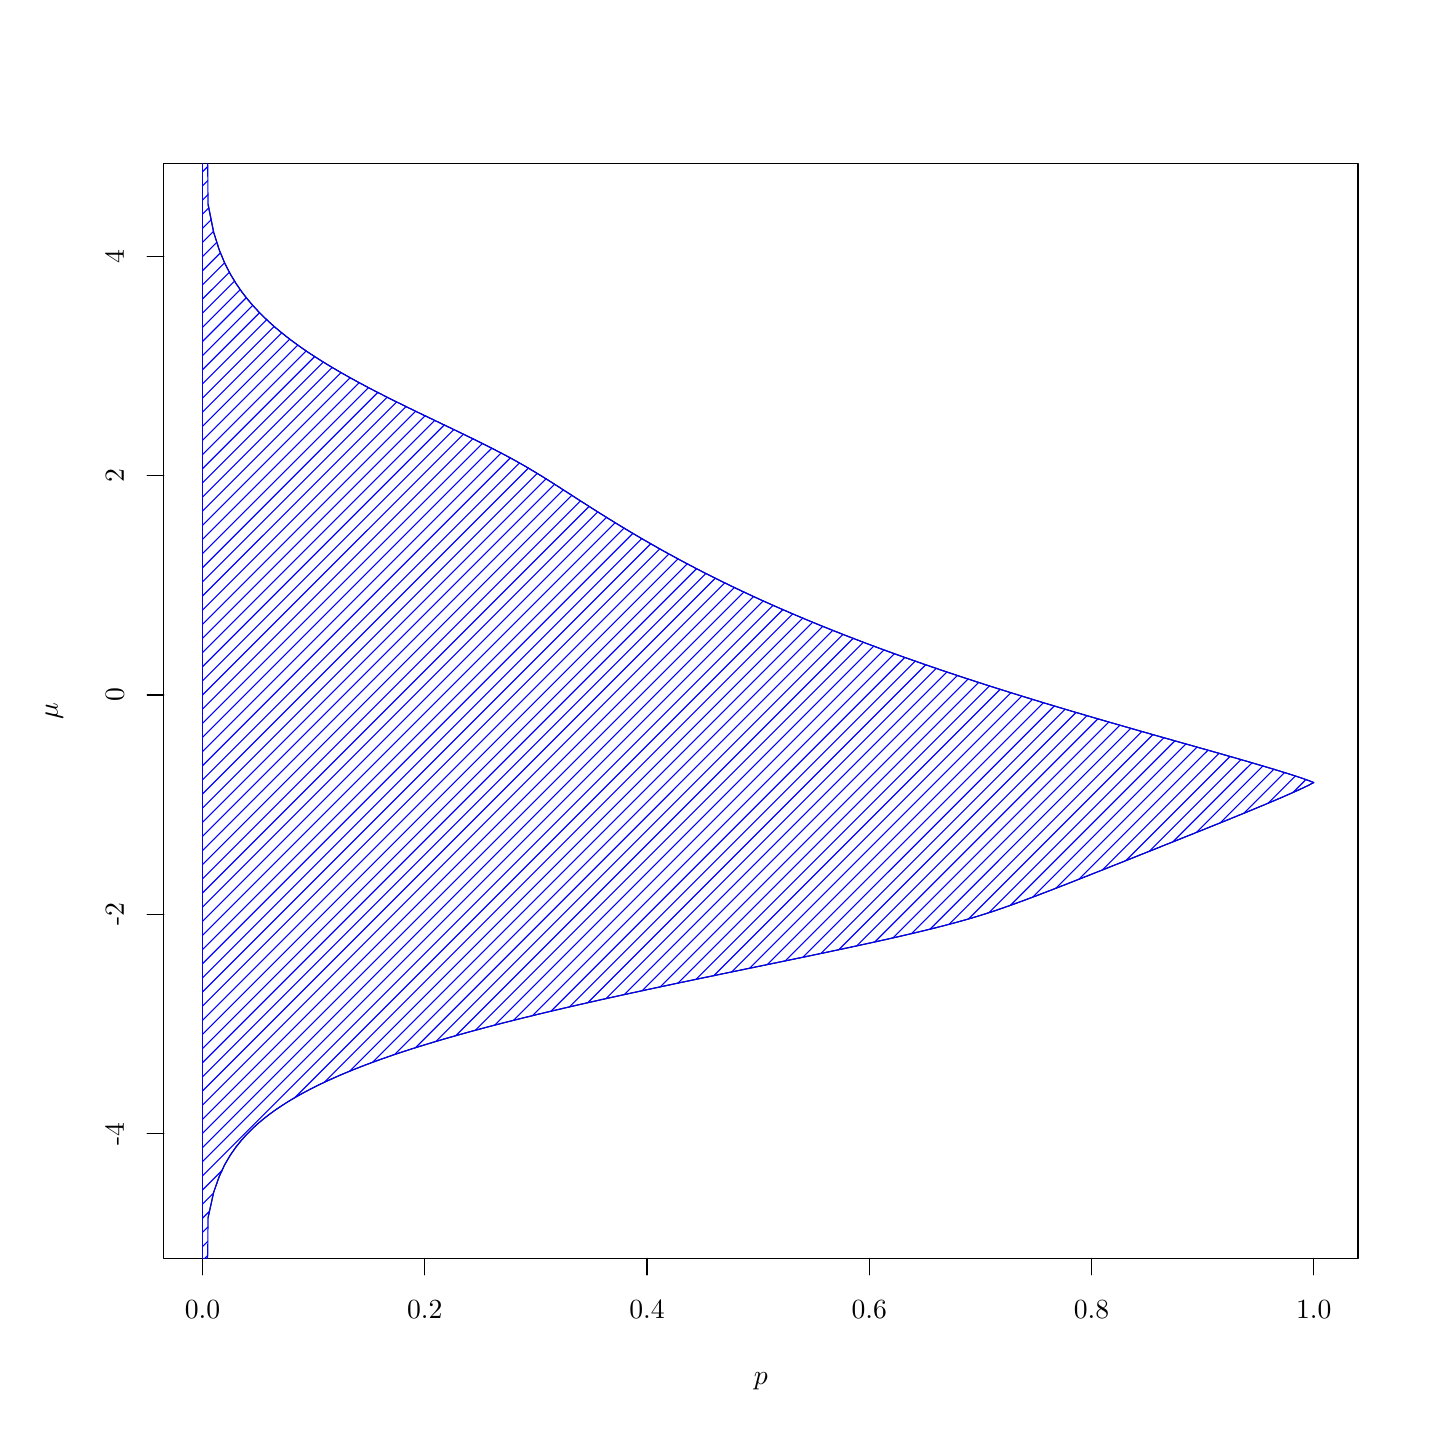
\begin{tikzpicture}[x=1pt,y=1pt]
\definecolor{fillColor}{RGB}{255,255,255}
\path[use as bounding box,fill=fillColor,fill opacity=0.00] (0,0) rectangle (505.89,505.89);
\begin{scope}
\path[clip] ( 49.20, 61.20) rectangle (480.69,456.69);
\definecolor{drawColor}{RGB}{0,0,0}

\path[draw=drawColor,line width= 0.4pt,line join=round,line cap=round] ( 65.18, 75.85) --
	( 67.19, 85.00) --
	( 69.20, 90.73) --
	( 71.20, 95.03) --
	( 73.21, 98.46) --
	( 75.22,101.35) --
	( 77.23,103.86) --
	( 79.23,106.08) --
	( 81.24,108.09) --
	( 83.25,109.92) --
	( 85.26,111.60) --
	( 87.27,113.16) --
	( 89.27,114.63) --
	( 91.28,116.00) --
	( 93.29,117.30) --
	( 95.30,118.53) --
	( 97.30,119.70) --
	( 99.31,120.82) --
	(101.32,121.89) --
	(103.33,122.92) --
	(105.33,123.92) --
	(107.34,124.88) --
	(109.35,125.80) --
	(111.36,126.70) --
	(113.37,127.57) --
	(115.37,128.41) --
	(117.38,129.23) --
	(119.39,130.03) --
	(121.40,130.81) --
	(123.40,131.57) --
	(125.41,132.31) --
	(127.42,133.04) --
	(129.43,133.74) --
	(131.43,134.44) --
	(133.44,135.12) --
	(135.45,135.79) --
	(137.46,136.44) --
	(139.47,137.09) --
	(141.47,137.72) --
	(143.48,138.34) --
	(145.49,138.95) --
	(147.50,139.56) --
	(149.50,140.15) --
	(151.51,140.74) --
	(153.52,141.31) --
	(155.53,141.88) --
	(157.53,142.44) --
	(159.54,143.00) --
	(161.55,143.54) --
	(163.56,144.08) --
	(165.56,144.62) --
	(167.57,145.15) --
	(169.58,145.67) --
	(171.59,146.19) --
	(173.60,146.70) --
	(175.60,147.20) --
	(177.61,147.71) --
	(179.62,148.20) --
	(181.63,148.69) --
	(183.63,149.18) --
	(185.64,149.67) --
	(187.65,150.15) --
	(189.66,150.62) --
	(191.66,151.09) --
	(193.67,151.56) --
	(195.68,152.03) --
	(197.69,152.49) --
	(199.70,152.95) --
	(201.70,153.41) --
	(203.71,153.86) --
	(205.72,154.31) --
	(207.73,154.76) --
	(209.73,155.21) --
	(211.74,155.65) --
	(213.75,156.09) --
	(215.76,156.53) --
	(217.76,156.97) --
	(219.77,157.40) --
	(221.78,157.83) --
	(223.79,158.27) --
	(225.80,158.69) --
	(227.80,159.12) --
	(229.81,159.55) --
	(231.82,159.97) --
	(233.83,160.40) --
	(235.83,160.82) --
	(237.84,161.24) --
	(239.85,161.66) --
	(241.86,162.08) --
	(243.86,162.50) --
	(245.87,162.91) --
	(247.88,163.33) --
	(249.89,163.75) --
	(251.90,164.16) --
	(253.90,164.58) --
	(255.91,164.99) --
	(257.92,165.41) --
	(259.93,165.82) --
	(261.93,166.23) --
	(263.94,166.65) --
	(265.95,167.06) --
	(267.96,167.47) --
	(269.96,167.89) --
	(271.97,168.30) --
	(273.98,168.72) --
	(275.99,169.13) --
	(277.99,169.55) --
	(280.00,169.96) --
	(282.01,170.38) --
	(284.02,170.80) --
	(286.03,171.22) --
	(288.03,171.64) --
	(290.04,172.06) --
	(292.05,172.49) --
	(294.06,172.91) --
	(296.06,173.34) --
	(298.07,173.77) --
	(300.08,174.20) --
	(302.09,174.64) --
	(304.09,175.07) --
	(306.10,175.51) --
	(308.11,175.96) --
	(310.12,176.40) --
	(312.13,176.86) --
	(314.13,177.31) --
	(316.14,177.77) --
	(318.15,178.24) --
	(320.16,178.71) --
	(322.16,179.19) --
	(324.17,179.67) --
	(326.18,180.16) --
	(328.19,180.66) --
	(330.19,181.17) --
	(332.20,181.69) --
	(334.21,182.22) --
	(336.22,182.77) --
	(338.23,183.33) --
	(340.23,183.90) --
	(342.24,184.49) --
	(344.25,185.11) --
	(346.26,185.74) --
	(348.26,186.39) --
	(350.27,187.06) --
	(352.28,187.75) --
	(354.29,188.45) --
	(356.29,189.17) --
	(358.30,189.90) --
	(360.31,190.64) --
	(362.32,191.39) --
	(364.33,192.14) --
	(366.33,192.91) --
	(368.34,193.68) --
	(370.35,194.45) --
	(372.36,195.23) --
	(374.36,196.01) --
	(376.37,196.80) --
	(378.38,197.59) --
	(380.39,198.38) --
	(382.39,199.17) --
	(384.40,199.96) --
	(386.41,200.76) --
	(388.42,201.56) --
	(390.42,202.35) --
	(392.43,203.15) --
	(394.44,203.95) --
	(396.45,204.75) --
	(398.46,205.55) --
	(400.46,206.35) --
	(402.47,207.15) --
	(404.48,207.95) --
	(406.49,208.75) --
	(408.49,209.55) --
	(410.50,210.36) --
	(412.51,211.16) --
	(414.52,211.96) --
	(416.52,212.76) --
	(418.53,213.57) --
	(420.54,214.37) --
	(422.55,215.18) --
	(424.56,215.98) --
	(426.56,216.79) --
	(428.57,217.60) --
	(430.58,218.41) --
	(432.59,219.22) --
	(434.59,220.03) --
	(436.60,220.85) --
	(438.61,221.67) --
	(440.62,222.49) --
	(442.62,223.31) --
	(444.63,224.15) --
	(446.64,224.98) --
	(448.65,225.82) --
	(450.66,226.67) --
	(452.66,227.53) --
	(454.67,228.40) --
	(456.68,229.28) --
	(458.69,230.18) --
	(460.69,231.10) --
	(462.70,232.06) --
	(464.71,233.11);
\end{scope}
\begin{scope}
\path[clip] (  0.00,  0.00) rectangle (505.89,505.89);
\definecolor{drawColor}{RGB}{0,0,0}

\path[draw=drawColor,line width= 0.4pt,line join=round,line cap=round] ( 63.17, 61.20) -- (464.71, 61.20);

\path[draw=drawColor,line width= 0.4pt,line join=round,line cap=round] ( 63.17, 61.20) -- ( 63.17, 55.20);

\path[draw=drawColor,line width= 0.4pt,line join=round,line cap=round] (143.48, 61.20) -- (143.48, 55.20);

\path[draw=drawColor,line width= 0.4pt,line join=round,line cap=round] (223.79, 61.20) -- (223.79, 55.20);

\path[draw=drawColor,line width= 0.4pt,line join=round,line cap=round] (304.09, 61.20) -- (304.09, 55.20);

\path[draw=drawColor,line width= 0.4pt,line join=round,line cap=round] (384.40, 61.20) -- (384.40, 55.20);

\path[draw=drawColor,line width= 0.4pt,line join=round,line cap=round] (464.71, 61.20) -- (464.71, 55.20);

\node[text=drawColor,anchor=base,inner sep=0pt, outer sep=0pt, scale=  1.00] at ( 63.17, 39.60) {0.0};

\node[text=drawColor,anchor=base,inner sep=0pt, outer sep=0pt, scale=  1.00] at (143.48, 39.60) {0.2};

\node[text=drawColor,anchor=base,inner sep=0pt, outer sep=0pt, scale=  1.00] at (223.79, 39.60) {0.4};

\node[text=drawColor,anchor=base,inner sep=0pt, outer sep=0pt, scale=  1.00] at (304.09, 39.60) {0.6};

\node[text=drawColor,anchor=base,inner sep=0pt, outer sep=0pt, scale=  1.00] at (384.40, 39.60) {0.8};

\node[text=drawColor,anchor=base,inner sep=0pt, outer sep=0pt, scale=  1.00] at (464.71, 39.60) {1.0};

\path[draw=drawColor,line width= 0.4pt,line join=round,line cap=round] ( 49.20,106.17) -- ( 49.20,423.30);

\path[draw=drawColor,line width= 0.4pt,line join=round,line cap=round] ( 49.20,106.17) -- ( 43.20,106.17);

\path[draw=drawColor,line width= 0.4pt,line join=round,line cap=round] ( 49.20,185.45) -- ( 43.20,185.45);

\path[draw=drawColor,line width= 0.4pt,line join=round,line cap=round] ( 49.20,264.74) -- ( 43.20,264.74);

\path[draw=drawColor,line width= 0.4pt,line join=round,line cap=round] ( 49.20,344.02) -- ( 43.20,344.02);

\path[draw=drawColor,line width= 0.4pt,line join=round,line cap=round] ( 49.20,423.30) -- ( 43.20,423.30);

\node[text=drawColor,rotate= 90.00,anchor=base,inner sep=0pt, outer sep=0pt, scale=  1.00] at ( 34.80,106.17) {-4};

\node[text=drawColor,rotate= 90.00,anchor=base,inner sep=0pt, outer sep=0pt, scale=  1.00] at ( 34.80,185.45) {-2};

\node[text=drawColor,rotate= 90.00,anchor=base,inner sep=0pt, outer sep=0pt, scale=  1.00] at ( 34.80,264.74) {0};

\node[text=drawColor,rotate= 90.00,anchor=base,inner sep=0pt, outer sep=0pt, scale=  1.00] at ( 34.80,344.02) {2};

\node[text=drawColor,rotate= 90.00,anchor=base,inner sep=0pt, outer sep=0pt, scale=  1.00] at ( 34.80,423.30) {4};

\path[draw=drawColor,line width= 0.4pt,line join=round,line cap=round] ( 49.20, 61.20) --
	(480.69, 61.20) --
	(480.69,456.69) --
	( 49.20,456.69) --
	( 49.20, 61.20);
\end{scope}
\begin{scope}
\path[clip] (  0.00,  0.00) rectangle (505.89,505.89);
\definecolor{drawColor}{RGB}{0,0,0}

\node[text=drawColor,anchor=base,inner sep=0pt, outer sep=0pt, scale=  1.00] at (264.94, 15.60) {$p$};

\node[text=drawColor,rotate= 90.00,anchor=base,inner sep=0pt, outer sep=0pt, scale=  1.00] at ( 10.80,258.94) {$\mu$};
\end{scope}
\begin{scope}
\path[clip] ( 49.20, 61.20) rectangle (480.69,456.69);
\definecolor{drawColor}{RGB}{0,0,0}

\path[draw=drawColor,line width= 0.4pt,line join=round,line cap=round] ( 65.18,442.04) --
	( 67.19,432.01) --
	( 69.20,425.64) --
	( 71.20,420.81) --
	( 73.21,416.88) --
	( 75.22,413.55) --
	( 77.23,410.62) --
	( 79.23,408.01) --
	( 81.24,405.64) --
	( 83.25,403.46) --
	( 85.26,401.42) --
	( 87.27,399.52) --
	( 89.27,397.73) --
	( 91.28,396.04) --
	( 93.29,394.42) --
	( 95.30,392.88) --
	( 97.30,391.40) --
	( 99.31,389.97) --
	(101.32,388.60) --
	(103.33,387.28) --
	(105.33,385.99) --
	(107.34,384.74) --
	(109.35,383.52) --
	(111.36,382.33) --
	(113.37,381.17) --
	(115.37,380.03) --
	(117.38,378.91) --
	(119.39,377.82) --
	(121.40,376.74) --
	(123.40,375.68) --
	(125.41,374.63) --
	(127.42,373.60) --
	(129.43,372.58) --
	(131.43,371.58) --
	(133.44,370.58) --
	(135.45,369.59) --
	(137.46,368.61) --
	(139.47,367.63) --
	(141.47,366.66) --
	(143.48,365.70) --
	(145.49,364.73) --
	(147.50,363.77) --
	(149.50,362.81) --
	(151.51,361.85) --
	(153.52,360.89) --
	(155.53,359.92) --
	(157.53,358.95) --
	(159.54,357.98) --
	(161.55,357.00) --
	(163.56,356.01) --
	(165.56,355.01) --
	(167.57,353.99) --
	(169.58,352.96) --
	(171.59,351.92) --
	(173.60,350.85) --
	(175.60,349.76) --
	(177.61,348.64) --
	(179.62,347.50) --
	(181.63,346.32) --
	(183.63,345.12) --
	(185.64,343.89) --
	(187.65,342.64) --
	(189.66,341.37) --
	(191.66,340.09) --
	(193.67,338.80) --
	(195.68,337.51) --
	(197.69,336.21) --
	(199.70,334.92) --
	(201.70,333.64) --
	(203.71,332.36) --
	(205.72,331.09) --
	(207.73,329.83) --
	(209.73,328.58) --
	(211.74,327.34) --
	(213.75,326.11) --
	(215.76,324.90) --
	(217.76,323.69) --
	(219.77,322.51) --
	(221.78,321.33) --
	(223.79,320.17) --
	(225.80,319.02) --
	(227.80,317.88) --
	(229.81,316.76) --
	(231.82,315.65) --
	(233.83,314.56) --
	(235.83,313.47) --
	(237.84,312.40) --
	(239.85,311.35) --
	(241.86,310.30) --
	(243.86,309.27) --
	(245.87,308.25) --
	(247.88,307.24) --
	(249.89,306.24) --
	(251.90,305.26) --
	(253.90,304.28) --
	(255.91,303.32) --
	(257.92,302.37) --
	(259.93,301.43) --
	(261.93,300.50) --
	(263.94,299.57) --
	(265.95,298.66) --
	(267.96,297.76) --
	(269.96,296.87) --
	(271.97,295.99) --
	(273.98,295.12) --
	(275.99,294.25) --
	(277.99,293.40) --
	(280.00,292.55) --
	(282.01,291.71) --
	(284.02,290.89) --
	(286.03,290.06) --
	(288.03,289.25) --
	(290.04,288.44) --
	(292.05,287.65) --
	(294.06,286.86) --
	(296.06,286.07) --
	(298.07,285.30) --
	(300.08,284.53) --
	(302.09,283.76) --
	(304.09,283.01) --
	(306.10,282.26) --
	(308.11,281.51) --
	(310.12,280.78) --
	(312.13,280.05) --
	(314.13,279.32) --
	(316.14,278.60) --
	(318.15,277.89) --
	(320.16,277.18) --
	(322.16,276.48) --
	(324.17,275.78) --
	(326.18,275.09) --
	(328.19,274.40) --
	(330.19,273.72) --
	(332.20,273.05) --
	(334.21,272.37) --
	(336.22,271.71) --
	(338.23,271.04) --
	(340.23,270.38) --
	(342.24,269.73) --
	(344.25,269.08) --
	(346.26,268.43) --
	(348.26,267.79) --
	(350.27,267.15) --
	(352.28,266.52) --
	(354.29,265.89) --
	(356.29,265.26) --
	(358.30,264.64) --
	(360.31,264.02) --
	(362.32,263.40) --
	(364.33,262.79) --
	(366.33,262.18) --
	(368.34,261.57) --
	(370.35,260.96) --
	(372.36,260.36) --
	(374.36,259.76) --
	(376.37,259.17) --
	(378.38,258.57) --
	(380.39,257.98) --
	(382.39,257.39) --
	(384.40,256.80) --
	(386.41,256.22) --
	(388.42,255.63) --
	(390.42,255.05) --
	(392.43,254.47) --
	(394.44,253.90) --
	(396.45,253.32) --
	(398.46,252.75) --
	(400.46,252.17) --
	(402.47,251.60) --
	(404.48,251.03) --
	(406.49,250.46) --
	(408.49,249.89) --
	(410.50,249.32) --
	(412.51,248.76) --
	(414.52,248.19) --
	(416.52,247.62) --
	(418.53,247.05) --
	(420.54,246.49) --
	(422.55,245.92) --
	(424.56,245.35) --
	(426.56,244.79) --
	(428.57,244.22) --
	(430.58,243.65) --
	(432.59,243.07) --
	(434.59,242.50) --
	(436.60,241.93) --
	(438.61,241.35) --
	(440.62,240.77) --
	(442.62,240.18) --
	(444.63,239.59) --
	(446.64,239.00) --
	(448.65,238.40) --
	(450.66,237.80) --
	(452.66,237.19) --
	(454.67,236.56) --
	(456.68,235.93) --
	(458.69,235.28) --
	(460.69,234.61) --
	(462.70,233.90) --
	(464.71,233.11);
\definecolor{drawColor}{RGB}{0,0,255}

\path[draw=drawColor,line width= 0.4pt,line join=round,line cap=round] ( 63.17,504.92) -- ( 64.14,505.89);

\path[draw=drawColor,line width= 0.4pt,line join=round,line cap=round] ( 63.17,499.81) -- ( 64.64,501.28);

\path[draw=drawColor,line width= 0.4pt,line join=round,line cap=round] ( 63.17,494.70) -- ( 64.68,496.21);

\path[draw=drawColor,line width= 0.4pt,line join=round,line cap=round] ( 63.17,489.59) -- ( 64.73,491.15);

\path[draw=drawColor,line width= 0.4pt,line join=round,line cap=round] ( 63.17,484.48) -- ( 64.78,486.08);

\path[draw=drawColor,line width= 0.4pt,line join=round,line cap=round] ( 63.17,479.37) -- ( 64.82,481.02);

\path[draw=drawColor,line width= 0.4pt,line join=round,line cap=round] ( 63.17,474.26) -- ( 64.87,475.96);

\path[draw=drawColor,line width= 0.4pt,line join=round,line cap=round] ( 63.17,469.15) -- ( 64.92,470.89);

\path[draw=drawColor,line width= 0.4pt,line join=round,line cap=round] ( 63.17,464.04) -- ( 64.96,465.83);

\path[draw=drawColor,line width= 0.4pt,line join=round,line cap=round] ( 63.17,458.93) -- ( 65.01,460.76);

\path[draw=drawColor,line width= 0.4pt,line join=round,line cap=round] ( 63.17,453.82) -- ( 65.06,455.70);

\path[draw=drawColor,line width= 0.4pt,line join=round,line cap=round] ( 63.17,448.71) -- ( 65.10,450.64);

\path[draw=drawColor,line width= 0.4pt,line join=round,line cap=round] ( 63.17,443.60) -- ( 65.15,445.57);

\path[draw=drawColor,line width= 0.4pt,line join=round,line cap=round] ( 63.17,438.49) -- ( 65.44,440.75);

\path[draw=drawColor,line width= 0.4pt,line join=round,line cap=round] ( 63.17,433.38) -- ( 66.29,436.49);

\path[draw=drawColor,line width= 0.4pt,line join=round,line cap=round] ( 63.17,428.27) -- ( 67.14,432.24);

\path[draw=drawColor,line width= 0.4pt,line join=round,line cap=round] ( 63.17,423.16) -- ( 68.35,428.33);

\path[draw=drawColor,line width= 0.4pt,line join=round,line cap=round] ( 63.17,418.05) -- ( 69.66,424.53);

\path[draw=drawColor,line width= 0.4pt,line join=round,line cap=round] ( 63.17,412.94) -- ( 71.16,420.92);

\path[draw=drawColor,line width= 0.4pt,line join=round,line cap=round] ( 63.17,407.83) -- ( 72.88,417.53);

\path[draw=drawColor,line width= 0.4pt,line join=round,line cap=round] ( 63.17,402.72) -- ( 74.76,414.31);

\path[draw=drawColor,line width= 0.4pt,line join=round,line cap=round] ( 63.17,397.60) -- ( 76.81,411.24);

\path[draw=drawColor,line width= 0.4pt,line join=round,line cap=round] ( 63.17,392.49) -- ( 79.00,408.32);

\path[draw=drawColor,line width= 0.4pt,line join=round,line cap=round] ( 63.17,387.38) -- ( 81.33,405.54);

\path[draw=drawColor,line width= 0.4pt,line join=round,line cap=round] ( 63.17,382.27) -- ( 83.80,402.90);

\path[draw=drawColor,line width= 0.4pt,line join=round,line cap=round] ( 63.17,377.16) -- ( 86.38,400.37);

\path[draw=drawColor,line width= 0.4pt,line join=round,line cap=round] ( 63.17,372.05) -- ( 89.05,397.93);

\path[draw=drawColor,line width= 0.4pt,line join=round,line cap=round] ( 63.17,366.94) -- ( 91.83,395.60);

\path[draw=drawColor,line width= 0.4pt,line join=round,line cap=round] ( 63.17,361.83) -- ( 94.69,393.35);

\path[draw=drawColor,line width= 0.4pt,line join=round,line cap=round] ( 63.17,356.72) -- ( 97.62,391.17);

\path[draw=drawColor,line width= 0.4pt,line join=round,line cap=round] ( 63.17,351.61) -- (100.63,389.07);

\path[draw=drawColor,line width= 0.4pt,line join=round,line cap=round] ( 63.17,346.50) -- (103.71,387.03);

\path[draw=drawColor,line width= 0.4pt,line join=round,line cap=round] ( 63.17,341.39) -- (106.84,385.05);

\path[draw=drawColor,line width= 0.4pt,line join=round,line cap=round] ( 63.17,336.28) -- (110.02,383.12);

\path[draw=drawColor,line width= 0.4pt,line join=round,line cap=round] ( 63.17,331.17) -- (113.24,381.24);

\path[draw=drawColor,line width= 0.4pt,line join=round,line cap=round] ( 63.17,326.06) -- (116.51,379.40);

\path[draw=drawColor,line width= 0.4pt,line join=round,line cap=round] ( 63.17,320.95) -- (119.81,377.59);

\path[draw=drawColor,line width= 0.4pt,line join=round,line cap=round] ( 63.17,315.84) -- (123.15,375.81);

\path[draw=drawColor,line width= 0.4pt,line join=round,line cap=round] ( 63.17,310.73) -- (126.51,374.07);

\path[draw=drawColor,line width= 0.4pt,line join=round,line cap=round] ( 63.17,305.62) -- (129.90,372.35);

\path[draw=drawColor,line width= 0.4pt,line join=round,line cap=round] ( 63.17,300.51) -- (133.31,370.64);

\path[draw=drawColor,line width= 0.4pt,line join=round,line cap=round] ( 63.17,295.40) -- (136.74,368.96);

\path[draw=drawColor,line width= 0.4pt,line join=round,line cap=round] ( 63.17,290.29) -- (140.17,367.29);

\path[draw=drawColor,line width= 0.4pt,line join=round,line cap=round] ( 63.17,285.18) -- (143.62,365.63);

\path[draw=drawColor,line width= 0.4pt,line join=round,line cap=round] ( 63.17,280.07) -- (147.08,363.97);

\path[draw=drawColor,line width= 0.4pt,line join=round,line cap=round] ( 63.17,274.96) -- (150.53,362.32);

\path[draw=drawColor,line width= 0.4pt,line join=round,line cap=round] ( 63.17,269.85) -- (153.99,360.66);

\path[draw=drawColor,line width= 0.4pt,line join=round,line cap=round] ( 63.17,264.74) -- (157.44,359.00);

\path[draw=drawColor,line width= 0.4pt,line join=round,line cap=round] ( 63.17,259.63) -- (160.87,357.33);

\path[draw=drawColor,line width= 0.4pt,line join=round,line cap=round] ( 63.17,254.52) -- (164.30,355.64);

\path[draw=drawColor,line width= 0.4pt,line join=round,line cap=round] ( 63.17,249.41) -- (167.70,353.93);

\path[draw=drawColor,line width= 0.4pt,line join=round,line cap=round] ( 63.17,244.30) -- (171.07,352.19);

\path[draw=drawColor,line width= 0.4pt,line join=round,line cap=round] ( 63.17,239.19) -- (174.40,350.41);

\path[draw=drawColor,line width= 0.4pt,line join=round,line cap=round] ( 63.17,234.08) -- (177.69,348.59);

\path[draw=drawColor,line width= 0.4pt,line join=round,line cap=round] ( 63.17,228.97) -- (180.93,346.73);

\path[draw=drawColor,line width= 0.4pt,line join=round,line cap=round] ( 63.17,223.86) -- (184.13,344.82);

\path[draw=drawColor,line width= 0.4pt,line join=round,line cap=round] ( 63.17,218.75) -- (187.29,342.86);

\path[draw=drawColor,line width= 0.4pt,line join=round,line cap=round] ( 63.17,213.64) -- (190.42,340.88);

\path[draw=drawColor,line width= 0.4pt,line join=round,line cap=round] ( 63.17,208.53) -- (193.54,338.89);

\path[draw=drawColor,line width= 0.4pt,line join=round,line cap=round] ( 63.17,203.42) -- (196.64,336.89);

\path[draw=drawColor,line width= 0.4pt,line join=round,line cap=round] ( 63.17,198.30) -- (199.75,334.89);

\path[draw=drawColor,line width= 0.4pt,line join=round,line cap=round] ( 63.17,193.19) -- (202.87,332.89);

\path[draw=drawColor,line width= 0.4pt,line join=round,line cap=round] ( 63.17,188.08) -- (206.00,330.91);

\path[draw=drawColor,line width= 0.4pt,line join=round,line cap=round] ( 63.17,182.97) -- (209.14,328.94);

\path[draw=drawColor,line width= 0.4pt,line join=round,line cap=round] ( 63.17,177.86) -- (212.30,326.99);

\path[draw=drawColor,line width= 0.4pt,line join=round,line cap=round] ( 63.17,172.75) -- (215.48,325.06);

\path[draw=drawColor,line width= 0.4pt,line join=round,line cap=round] ( 63.17,167.64) -- (218.68,323.15);

\path[draw=drawColor,line width= 0.4pt,line join=round,line cap=round] ( 63.17,162.53) -- (221.90,321.26);

\path[draw=drawColor,line width= 0.4pt,line join=round,line cap=round] ( 63.17,157.42) -- (225.14,319.39);

\path[draw=drawColor,line width= 0.4pt,line join=round,line cap=round] ( 63.17,152.31) -- (228.41,317.55);

\path[draw=drawColor,line width= 0.4pt,line join=round,line cap=round] ( 63.17,147.20) -- (231.69,315.72);

\path[draw=drawColor,line width= 0.4pt,line join=round,line cap=round] ( 63.17,142.09) -- (235.00,313.92);

\path[draw=drawColor,line width= 0.4pt,line join=round,line cap=round] ( 63.17,136.98) -- (238.34,312.14);

\path[draw=drawColor,line width= 0.4pt,line join=round,line cap=round] ( 63.17,131.87) -- (241.69,310.39);

\path[draw=drawColor,line width= 0.4pt,line join=round,line cap=round] ( 63.17,126.76) -- (245.07,308.66);

\path[draw=drawColor,line width= 0.4pt,line join=round,line cap=round] ( 63.17,121.65) -- (248.47,306.95);

\path[draw=drawColor,line width= 0.4pt,line join=round,line cap=round] ( 63.17,116.54) -- (251.89,305.26);

\path[draw=drawColor,line width= 0.4pt,line join=round,line cap=round] ( 63.17,111.43) -- (255.34,303.60);

\path[draw=drawColor,line width= 0.4pt,line join=round,line cap=round] ( 63.17,106.32) -- (258.81,301.95);

\path[draw=drawColor,line width= 0.4pt,line join=round,line cap=round] ( 63.17,101.21) -- (262.29,300.33);

\path[draw=drawColor,line width= 0.4pt,line join=round,line cap=round] ( 63.17, 96.10) -- (265.80,298.73);

\path[draw=drawColor,line width= 0.4pt,line join=round,line cap=round] ( 63.17, 90.99) -- (269.34,297.15);

\path[draw=drawColor,line width= 0.4pt,line join=round,line cap=round] ( 63.17, 85.88) -- ( 70.23, 92.93);

\path[draw=drawColor,line width= 0.4pt,line join=round,line cap=round] ( 96.55,119.26) -- (272.89,295.59);

\path[draw=drawColor,line width= 0.4pt,line join=round,line cap=round] ( 63.17, 80.77) -- ( 67.13, 84.72);

\path[draw=drawColor,line width= 0.4pt,line join=round,line cap=round] (107.23,124.82) -- (276.46,294.05);

\path[draw=drawColor,line width= 0.4pt,line join=round,line cap=round] ( 63.17, 75.66) -- ( 65.69, 78.18);

\path[draw=drawColor,line width= 0.4pt,line join=round,line cap=round] (116.31,128.79) -- (280.05,292.53);

\path[draw=drawColor,line width= 0.4pt,line join=round,line cap=round] ( 63.17, 70.55) -- ( 65.15, 72.52);

\path[draw=drawColor,line width= 0.4pt,line join=round,line cap=round] (124.66,132.03) -- (283.66,291.03);

\path[draw=drawColor,line width= 0.4pt,line join=round,line cap=round] ( 63.17, 65.44) -- ( 65.10, 67.36);

\path[draw=drawColor,line width= 0.4pt,line join=round,line cap=round] (132.56,134.82) -- (287.29,289.55);

\path[draw=drawColor,line width= 0.4pt,line join=round,line cap=round] ( 63.17, 60.33) -- ( 65.05, 62.20);

\path[draw=drawColor,line width= 0.4pt,line join=round,line cap=round] (140.15,137.30) -- (290.93,288.09);

\path[draw=drawColor,line width= 0.4pt,line join=round,line cap=round] ( 63.17, 55.22) -- ( 65.00, 57.04);

\path[draw=drawColor,line width= 0.4pt,line join=round,line cap=round] (147.52,139.56) -- (294.60,286.64);

\path[draw=drawColor,line width= 0.4pt,line join=round,line cap=round] ( 63.17, 50.11) -- ( 64.95, 51.88);

\path[draw=drawColor,line width= 0.4pt,line join=round,line cap=round] (154.72,141.65) -- (298.28,285.22);

\path[draw=drawColor,line width= 0.4pt,line join=round,line cap=round] ( 63.17, 45.00) -- ( 64.90, 46.72);

\path[draw=drawColor,line width= 0.4pt,line join=round,line cap=round] (161.78,143.61) -- (301.98,283.80);

\path[draw=drawColor,line width= 0.4pt,line join=round,line cap=round] ( 63.17, 39.89) -- ( 64.85, 41.56);

\path[draw=drawColor,line width= 0.4pt,line join=round,line cap=round] (168.74,145.45) -- (305.70,282.41);

\path[draw=drawColor,line width= 0.4pt,line join=round,line cap=round] ( 63.17, 34.78) -- ( 64.80, 36.40);

\path[draw=drawColor,line width= 0.4pt,line join=round,line cap=round] (175.60,147.20) -- (309.43,281.03);

\path[draw=drawColor,line width= 0.4pt,line join=round,line cap=round] ( 63.17, 29.67) -- ( 64.75, 31.24);

\path[draw=drawColor,line width= 0.4pt,line join=round,line cap=round] (182.39,148.88) -- (313.17,279.67);

\path[draw=drawColor,line width= 0.4pt,line join=round,line cap=round] ( 63.17, 24.56) -- ( 64.70, 26.08);

\path[draw=drawColor,line width= 0.4pt,line join=round,line cap=round] (189.11,150.49) -- (316.94,278.32);

\path[draw=drawColor,line width= 0.4pt,line join=round,line cap=round] ( 63.17, 19.45) -- ( 64.65, 20.92);

\path[draw=drawColor,line width= 0.4pt,line join=round,line cap=round] (195.78,152.05) -- (320.71,276.99);

\path[draw=drawColor,line width= 0.4pt,line join=round,line cap=round] ( 63.17, 14.34) -- ( 64.60, 15.76);

\path[draw=drawColor,line width= 0.4pt,line join=round,line cap=round] (202.41,153.57) -- (324.51,275.67);

\path[draw=drawColor,line width= 0.4pt,line join=round,line cap=round] ( 63.17,  9.23) -- ( 64.55, 10.60);

\path[draw=drawColor,line width= 0.4pt,line join=round,line cap=round] (208.99,155.04) -- (328.31,274.36);

\path[draw=drawColor,line width= 0.4pt,line join=round,line cap=round] ( 63.17,  4.11) -- ( 64.50,  5.44);

\path[draw=drawColor,line width= 0.4pt,line join=round,line cap=round] (215.54,156.48) -- (332.13,273.07);

\path[draw=drawColor,line width= 0.4pt,line join=round,line cap=round] ( 64.17,  0.00) -- ( 64.45,  0.28);

\path[draw=drawColor,line width= 0.4pt,line join=round,line cap=round] (222.06,157.90) -- (335.96,271.79);

\path[draw=drawColor,line width= 0.4pt,line join=round,line cap=round] (228.56,159.28) -- (339.80,270.53);

\path[draw=drawColor,line width= 0.4pt,line join=round,line cap=round] (235.04,160.65) -- (343.66,269.27);

\path[draw=drawColor,line width= 0.4pt,line join=round,line cap=round] (241.51,162.01) -- (347.53,268.03);

\path[draw=drawColor,line width= 0.4pt,line join=round,line cap=round] (247.96,163.35) -- (351.40,266.80);

\path[draw=drawColor,line width= 0.4pt,line join=round,line cap=round] (254.40,164.68) -- (355.29,265.57);

\path[draw=drawColor,line width= 0.4pt,line join=round,line cap=round] (260.84,166.01) -- (359.19,264.36);

\path[draw=drawColor,line width= 0.4pt,line join=round,line cap=round] (267.27,167.33) -- (363.10,263.16);

\path[draw=drawColor,line width= 0.4pt,line join=round,line cap=round] (273.71,168.66) -- (367.02,261.97);

\path[draw=drawColor,line width= 0.4pt,line join=round,line cap=round] (280.16,170.00) -- (370.95,260.78);

\path[draw=drawColor,line width= 0.4pt,line join=round,line cap=round] (286.61,171.34) -- (374.88,259.61);

\path[draw=drawColor,line width= 0.4pt,line join=round,line cap=round] (293.09,172.71) -- (378.82,258.44);

\path[draw=drawColor,line width= 0.4pt,line join=round,line cap=round] (299.59,174.09) -- (382.77,257.28);

\path[draw=drawColor,line width= 0.4pt,line join=round,line cap=round] (306.12,175.52) -- (386.73,256.13);

\path[draw=drawColor,line width= 0.4pt,line join=round,line cap=round] (312.70,176.99) -- (390.69,254.98);

\path[draw=drawColor,line width= 0.4pt,line join=round,line cap=round] (319.34,178.52) -- (394.66,253.83);

\path[draw=drawColor,line width= 0.4pt,line join=round,line cap=round] (326.07,180.13) -- (398.63,252.70);

\path[draw=drawColor,line width= 0.4pt,line join=round,line cap=round] (332.93,181.88) -- (402.61,251.56);

\path[draw=drawColor,line width= 0.4pt,line join=round,line cap=round] (339.98,183.83) -- (406.59,250.43);

\path[draw=drawColor,line width= 0.4pt,line join=round,line cap=round] (347.36,186.10) -- (410.57,249.30);

\path[draw=drawColor,line width= 0.4pt,line join=round,line cap=round] (355.12,188.75) -- (414.55,248.18);

\path[draw=drawColor,line width= 0.4pt,line join=round,line cap=round] (363.21,191.72) -- (418.54,247.05);

\path[draw=drawColor,line width= 0.4pt,line join=round,line cap=round] (371.49,194.90) -- (422.52,245.93);

\path[draw=drawColor,line width= 0.4pt,line join=round,line cap=round] (379.88,198.18) -- (426.51,244.80);

\path[draw=drawColor,line width= 0.4pt,line join=round,line cap=round] (388.34,201.53) -- (430.49,243.67);

\path[draw=drawColor,line width= 0.4pt,line join=round,line cap=round] (396.83,204.90) -- (434.46,242.54);

\path[draw=drawColor,line width= 0.4pt,line join=round,line cap=round] (405.32,208.29) -- (438.43,241.40);

\path[draw=drawColor,line width= 0.4pt,line join=round,line cap=round] (413.83,211.69) -- (442.40,240.25);

\path[draw=drawColor,line width= 0.4pt,line join=round,line cap=round] (422.35,215.10) -- (446.34,239.09);

\path[draw=drawColor,line width= 0.4pt,line join=round,line cap=round] (430.90,218.54) -- (450.28,237.91);

\path[draw=drawColor,line width= 0.4pt,line join=round,line cap=round] (439.51,222.04) -- (454.19,236.71);

\path[draw=drawColor,line width= 0.4pt,line join=round,line cap=round] (448.24,225.65) -- (458.07,235.48);

\path[draw=drawColor,line width= 0.4pt,line join=round,line cap=round] (457.22,229.52) -- (461.88,234.19);

\path[draw=drawColor,line width= 0.4pt,line join=round,line cap=round] ( 64.45,  0.00) --
	( 65.18, 75.85) --
	( 67.19, 85.00) --
	( 69.20, 90.73) --
	( 71.20, 95.03) --
	( 73.21, 98.46) --
	( 75.22,101.35) --
	( 77.23,103.86) --
	( 79.23,106.08) --
	( 81.24,108.09) --
	( 83.25,109.92) --
	( 85.26,111.60) --
	( 87.27,113.16) --
	( 89.27,114.63) --
	( 91.28,116.00) --
	( 93.29,117.30) --
	( 95.30,118.53) --
	( 97.30,119.70) --
	( 99.31,120.82) --
	(101.32,121.89) --
	(103.33,122.92) --
	(105.33,123.92) --
	(107.34,124.88) --
	(109.35,125.80) --
	(111.36,126.70) --
	(113.37,127.57) --
	(115.37,128.41) --
	(117.38,129.23) --
	(119.39,130.03) --
	(121.40,130.81) --
	(123.40,131.57) --
	(125.41,132.31) --
	(127.42,133.04) --
	(129.43,133.74) --
	(131.43,134.44) --
	(133.44,135.12) --
	(135.45,135.79) --
	(137.46,136.44) --
	(139.47,137.09) --
	(141.47,137.72) --
	(143.48,138.34) --
	(145.49,138.95) --
	(147.50,139.56) --
	(149.50,140.15) --
	(151.51,140.74) --
	(153.52,141.31) --
	(155.53,141.88) --
	(157.53,142.44) --
	(159.54,143.00) --
	(161.55,143.54) --
	(163.56,144.08) --
	(165.56,144.62) --
	(167.57,145.15) --
	(169.58,145.67) --
	(171.59,146.19) --
	(173.60,146.70) --
	(175.60,147.20) --
	(177.61,147.71) --
	(179.62,148.20) --
	(181.63,148.69) --
	(183.63,149.18) --
	(185.64,149.67) --
	(187.65,150.15) --
	(189.66,150.62) --
	(191.66,151.09) --
	(193.67,151.56) --
	(195.68,152.03) --
	(197.69,152.49) --
	(199.70,152.95) --
	(201.70,153.41) --
	(203.71,153.86) --
	(205.72,154.31) --
	(207.73,154.76) --
	(209.73,155.21) --
	(211.74,155.65) --
	(213.75,156.09) --
	(215.76,156.53) --
	(217.76,156.97) --
	(219.77,157.40) --
	(221.78,157.83) --
	(223.79,158.27) --
	(225.80,158.69) --
	(227.80,159.12) --
	(229.81,159.55) --
	(231.82,159.97) --
	(233.83,160.40) --
	(235.83,160.82) --
	(237.84,161.24) --
	(239.85,161.66) --
	(241.86,162.08) --
	(243.86,162.50) --
	(245.87,162.91) --
	(247.88,163.33) --
	(249.89,163.75) --
	(251.90,164.16) --
	(253.90,164.58) --
	(255.91,164.99) --
	(257.92,165.41) --
	(259.93,165.82) --
	(261.93,166.23) --
	(263.94,166.65) --
	(265.95,167.06) --
	(267.96,167.47) --
	(269.96,167.89) --
	(271.97,168.30) --
	(273.98,168.72) --
	(275.99,169.13) --
	(277.99,169.55) --
	(280.00,169.96) --
	(282.01,170.38) --
	(284.02,170.80) --
	(286.03,171.22) --
	(288.03,171.64) --
	(290.04,172.06) --
	(292.05,172.49) --
	(294.06,172.91) --
	(296.06,173.34) --
	(298.07,173.77) --
	(300.08,174.20) --
	(302.09,174.64) --
	(304.09,175.07) --
	(306.10,175.51) --
	(308.11,175.96) --
	(310.12,176.40) --
	(312.13,176.86) --
	(314.13,177.31) --
	(316.14,177.77) --
	(318.15,178.24) --
	(320.16,178.71) --
	(322.16,179.19) --
	(324.17,179.67) --
	(326.18,180.16) --
	(328.19,180.66) --
	(330.19,181.17) --
	(332.20,181.69) --
	(334.21,182.22) --
	(336.22,182.77) --
	(338.23,183.33) --
	(340.23,183.90) --
	(342.24,184.49) --
	(344.25,185.11) --
	(346.26,185.74) --
	(348.26,186.39) --
	(350.27,187.06) --
	(352.28,187.75) --
	(354.29,188.45) --
	(356.29,189.17) --
	(358.30,189.90) --
	(360.31,190.64) --
	(362.32,191.39) --
	(364.33,192.14) --
	(366.33,192.91) --
	(368.34,193.68) --
	(370.35,194.45) --
	(372.36,195.23) --
	(374.36,196.01) --
	(376.37,196.80) --
	(378.38,197.59) --
	(380.39,198.38) --
	(382.39,199.17) --
	(384.40,199.96) --
	(386.41,200.76) --
	(388.42,201.56) --
	(390.42,202.35) --
	(392.43,203.15) --
	(394.44,203.95) --
	(396.45,204.75) --
	(398.46,205.55) --
	(400.46,206.35) --
	(402.47,207.15) --
	(404.48,207.95) --
	(406.49,208.75) --
	(408.49,209.55) --
	(410.50,210.36) --
	(412.51,211.16) --
	(414.52,211.96) --
	(416.52,212.76) --
	(418.53,213.57) --
	(420.54,214.37) --
	(422.55,215.18) --
	(424.56,215.98) --
	(426.56,216.79) --
	(428.57,217.60) --
	(430.58,218.41) --
	(432.59,219.22) --
	(434.59,220.03) --
	(436.60,220.85) --
	(438.61,221.67) --
	(440.62,222.49) --
	(442.62,223.31) --
	(444.63,224.15) --
	(446.64,224.98) --
	(448.65,225.82) --
	(450.66,226.67) --
	(452.66,227.53) --
	(454.67,228.40) --
	(456.68,229.28) --
	(458.69,230.18) --
	(460.69,231.10) --
	(462.70,232.06) --
	(464.71,233.11) --
	(464.71,233.11) --
	(462.70,233.90) --
	(460.69,234.61) --
	(458.69,235.28) --
	(456.68,235.93) --
	(454.67,236.56) --
	(452.66,237.19) --
	(450.66,237.80) --
	(448.65,238.40) --
	(446.64,239.00) --
	(444.63,239.59) --
	(442.62,240.18) --
	(440.62,240.77) --
	(438.61,241.35) --
	(436.60,241.93) --
	(434.59,242.50) --
	(432.59,243.07) --
	(430.58,243.65) --
	(428.57,244.22) --
	(426.56,244.79) --
	(424.56,245.35) --
	(422.55,245.92) --
	(420.54,246.49) --
	(418.53,247.05) --
	(416.52,247.62) --
	(414.52,248.19) --
	(412.51,248.76) --
	(410.50,249.32) --
	(408.49,249.89) --
	(406.49,250.46) --
	(404.48,251.03) --
	(402.47,251.60) --
	(400.46,252.17) --
	(398.46,252.75) --
	(396.45,253.32) --
	(394.44,253.90) --
	(392.43,254.47) --
	(390.42,255.05) --
	(388.42,255.63) --
	(386.41,256.22) --
	(384.40,256.80) --
	(382.39,257.39) --
	(380.39,257.98) --
	(378.38,258.57) --
	(376.37,259.17) --
	(374.36,259.76) --
	(372.36,260.36) --
	(370.35,260.96) --
	(368.34,261.57) --
	(366.33,262.18) --
	(364.33,262.79) --
	(362.32,263.40) --
	(360.31,264.02) --
	(358.30,264.64) --
	(356.29,265.26) --
	(354.29,265.89) --
	(352.28,266.52) --
	(350.27,267.15) --
	(348.26,267.79) --
	(346.26,268.43) --
	(344.25,269.08) --
	(342.24,269.73) --
	(340.23,270.38) --
	(338.23,271.04) --
	(336.22,271.71) --
	(334.21,272.37) --
	(332.20,273.05) --
	(330.19,273.72) --
	(328.19,274.40) --
	(326.18,275.09) --
	(324.17,275.78) --
	(322.16,276.48) --
	(320.16,277.18) --
	(318.15,277.89) --
	(316.14,278.60) --
	(314.13,279.32) --
	(312.13,280.05) --
	(310.12,280.78) --
	(308.11,281.51) --
	(306.10,282.26) --
	(304.09,283.01) --
	(302.09,283.76) --
	(300.08,284.53) --
	(298.07,285.30) --
	(296.06,286.07) --
	(294.06,286.86) --
	(292.05,287.65) --
	(290.04,288.44) --
	(288.03,289.25) --
	(286.03,290.06) --
	(284.02,290.89) --
	(282.01,291.71) --
	(280.00,292.55) --
	(277.99,293.40) --
	(275.99,294.25) --
	(273.98,295.12) --
	(271.97,295.99) --
	(269.96,296.87) --
	(267.96,297.76) --
	(265.95,298.66) --
	(263.94,299.57) --
	(261.93,300.50) --
	(259.93,301.43) --
	(257.92,302.37) --
	(255.91,303.32) --
	(253.90,304.28) --
	(251.90,305.26) --
	(249.89,306.24) --
	(247.88,307.24) --
	(245.87,308.25) --
	(243.86,309.27) --
	(241.86,310.30) --
	(239.85,311.35) --
	(237.84,312.40) --
	(235.83,313.47) --
	(233.83,314.56) --
	(231.82,315.65) --
	(229.81,316.76) --
	(227.80,317.88) --
	(225.80,319.02) --
	(223.79,320.17) --
	(221.78,321.33) --
	(219.77,322.51) --
	(217.76,323.69) --
	(215.76,324.90) --
	(213.75,326.11) --
	(211.74,327.34) --
	(209.73,328.58) --
	(207.73,329.83) --
	(205.72,331.09) --
	(203.71,332.36) --
	(201.70,333.64) --
	(199.70,334.92) --
	(197.69,336.21) --
	(195.68,337.51) --
	(193.67,338.80) --
	(191.66,340.09) --
	(189.66,341.37) --
	(187.65,342.64) --
	(185.64,343.89) --
	(183.63,345.12) --
	(181.63,346.32) --
	(179.62,347.50) --
	(177.61,348.64) --
	(175.60,349.76) --
	(173.60,350.85) --
	(171.59,351.92) --
	(169.58,352.96) --
	(167.57,353.99) --
	(165.56,355.01) --
	(163.56,356.01) --
	(161.55,357.00) --
	(159.54,357.98) --
	(157.53,358.95) --
	(155.53,359.92) --
	(153.52,360.89) --
	(151.51,361.85) --
	(149.50,362.81) --
	(147.50,363.77) --
	(145.49,364.73) --
	(143.48,365.70) --
	(141.47,366.66) --
	(139.47,367.63) --
	(137.46,368.61) --
	(135.45,369.59) --
	(133.44,370.58) --
	(131.43,371.58) --
	(129.43,372.58) --
	(127.42,373.60) --
	(125.41,374.63) --
	(123.40,375.68) --
	(121.40,376.74) --
	(119.39,377.82) --
	(117.38,378.91) --
	(115.37,380.03) --
	(113.37,381.17) --
	(111.36,382.33) --
	(109.35,383.52) --
	(107.34,384.74) --
	(105.33,385.99) --
	(103.33,387.28) --
	(101.32,388.60) --
	( 99.31,389.97) --
	( 97.30,391.40) --
	( 95.30,392.88) --
	( 93.29,394.42) --
	( 91.28,396.04) --
	( 89.27,397.73) --
	( 87.27,399.52) --
	( 85.26,401.42) --
	( 83.25,403.46) --
	( 81.24,405.64) --
	( 79.23,408.01) --
	( 77.23,410.62) --
	( 75.22,413.55) --
	( 73.21,416.88) --
	( 71.20,420.81) --
	( 69.20,425.64) --
	( 67.19,432.01) --
	( 65.18,442.04) --
	( 64.60,505.89);

\path[draw=drawColor,line width= 0.4pt,line join=round,line cap=round] ( 63.17,505.89) --
	( 63.17,  0.00);
\end{scope}
\end{tikzpicture}

}
\end{figure}

\note{As $p$ approaches 1, the mean of $H$ is more tightly constrained: must be close to the mean of the observed distribution $F$, namely $-0.8$. As $p$ approaches zero, it is less and less constrained: since it contributes very little to the overall mixture, it can take on nearly any mean.}

\end{frame}
%%%%%%%%%%%%%%%%%%%%%%%%%%%%%%%%%%%%%%%%%%%%%%%%%%%%
\begin{frame}
  \frametitle{Restrictions from Non-differential Mis-classification}

  %\begin{block}{Equivalent Problem}
  %  \small
  %  Given a specified CDF $F$, for what values of $p$ and $\mu$ do there exist valid CDFs $(G,H)$ with $F = (1 - p) G + p H$ and $\mu = \mbox{mean}(H)$? 
%\end{block}

  \begin{alertblock}{Necessary and Sufficient Condition if $F$ is Continuous}
    \small
   \[
     \int_{-\infty}^{F^{-1}(p)} \frac{x}{p}\; f(x) \; dx \leq \;  \mu \; \leq \int_{F^{-1}(1-p)}^{+\infty} \frac{x}{p} \; f(x)\; dx
   \]
  \end{alertblock}

  \begin{block}{Back to Our Original Problem}
    \small
    \vspace{-1em}
    \begin{itemize}
      \item Observe $F_{tk}$ for all $(t,k)$ 
      \item $r_{tk}$ pinned down by $(\alpha_0, \alpha_1)$
      \item Can we find $F_{tk}^{t^*}$ so that $F_{tk} = (1 - r_{tk})F_{tk}^0 + r_{tk} F_{tk}^1$?
      \item Non-diff.\ assumption $\Rightarrow$ mean of $F_{tk}^1$ pinned down by $(\alpha_0, \alpha_1)$.
      \item Implies joint restrictions on $(\alpha_0,\alpha_1)$, hence $\beta$.
    \end{itemize}
  \end{block}


  \note{I just showed you necessary conditions, but it turns out that they're also sufficient if $F$ is continuous, so we've solved the problem of when a valid mixture decomposition exists. How does this relate to the original question: does non-differential measurement error further restrict $\alpha_0,\alpha_1$?}



\end{frame}
%%%%%%%%%%%%%%%%%%%%%%%%%%%%%%%%%%%%%%%%%%%%%%%%%%%%
\begin{frame}
  \frametitle{Sharp Identified Set under Baseline Assumptions}

  \begin{alertblock}{Theorem}
    Under baseline assumptions, sharp identified set for $\beta(\mathbf{x})$ is never a singleton, regardless of how many (discrete) values $z$ takes on.
  \end{alertblock}

  \begin{block}{Intuition}
    No mis-classification $\Rightarrow r_{tk} = 0 \mbox{ or } 1$ and we can always form a valid mixture in this case. Show that Wald estimand always lies within the sharp identified set for $\beta$. 
  \end{block}


  \note{Second contribution. Simple bounds I showed you earlier are not sharp: in other words, they're not the best bounds you can get under our assumptions. Even when we get the best bounds (the ``sharp'' bounds) they're not enough to point identify $\beta$. Also want to point out that the restrictions from non-differential measurement error can be very informative in practice! Now transition to point identification argument. Can we obtain point identification under stronger but credible assumptions?}

\end{frame}
%%%%%%%%%%%%%%%%%%%%%%%%%%%%%%%%%%%%%%%%%%%%%%%%%%%%
\begin{frame}
  \frametitle{Point Identification: 1st Ingredient}


  \vspace{-1em}

  \begin{block}{Reparameterization}
    \vspace{-1em}
\begin{align*}
  \theta_1(\mathbf{x}) &= \beta(\mathbf{x})/\left[ 1 - \alpha_0(\mathbf{x}) - \mathbf{\alpha}_1(\mathbf{x})  \right]\\
  \theta_2(\mathbf{x}) &= \left[\theta_1(\mathbf{x})\right]^2 \left[ 1 + \alpha_0(\mathbf{x}) - \alpha_1(\mathbf{x})\right] \\
  \theta_3(\mathbf{x}) &= \left[\theta_1(\mathbf{x})\right]^3\left[ \left\{ 1 - \alpha_0(\mathbf{x}) - \alpha_1(\mathbf{x}) \right\}^2 + 6\alpha_0(\mathbf{x})\left\{ 1 - \alpha_1(\mathbf{x}) \right\} \right]
\end{align*}

\[\boxed{\beta(\mathbf{x}) = 0 \iff \theta_1(\mathbf{x}) = \theta_2(\mathbf{x}) = \theta_3(\mathbf{x}) = 0}\]
  \end{block}

  \vspace{-1.5em}

  \begin{block}{Lemma}
    Baseline Assumptions $\implies \alert{\mbox{Cov}(y,z|\mathbf{x}) = \theta_1(\mathbf{x}) \mbox{Cov}(z,T|\mathbf{x})}$.
  \end{block}

\end{frame}
%%%%%%%%%%%%%%%%%%%%%%%%%%%%%%%%%%%%%%
\begin{frame}
  \frametitle{Point Identification: 2nd Ingredient}

  \begin{block}{Assumption (II)}
    $\mathbb{E}[\varepsilon^2|\mathbf{x},z] = \mathbb{E}[\varepsilon^2|\mathbf{x}]$
  \end{block}

  \begin{block}{Lemma}
    (Baseline) + (II) $\implies$ 
    \[
      \alert{\mbox{Cov}(y^2,z|\mathbf{x}) = 2\mbox{Cov}(yT,z|\mathbf{x}) \theta_1(\mathbf{x}) -\mbox{Cov}(T,z|\mathbf{x})\theta_2(\mathbf{x})}
    \]
  \end{block}

  \begin{block}{Corollary}
    (Baseline) + (II) + $[\beta(\mathbf{x})\neq 0] \implies \left[ \alpha_1(\mathbf{x}) - \alpha_0(\mathbf{x}) \right]$ is identified. Hence, $\beta(\mathbf{x})$ is identified if mis-classification is one-sided.
  \end{block}
    

  
\end{frame}
%%%%%%%%%%%%%%%%%%%%%%%%%%%%%%%%%%%%%%
\begin{frame}
  \frametitle{Point Identification: 3rd Ingredient}

  \begin{block}{Assumption (III)}
    \begin{enumerate}[(i)]
    \item $\mathbb{E}[\varepsilon^2|\mathbf{x},z,T^*,T] = \mathbb{E}[\varepsilon^2|\mathbf{x},z, T^*]$
    \item $\mathbb{E}[\varepsilon^3|\mathbf{x},z] = \mathbb{E}[\varepsilon^3|\mathbf{x}]$
  \end{enumerate}
  \end{block}
 
  \begin{block}{Lemma}
    (Baseline) + (II) + (III) $\implies$ 
  \small
\[
  \alert{\mbox{Cov}(y^3,z|\mathbf{x}) = 3 \mbox{Cov}(y^2T,z|\mathbf{x}) \theta_1(\mathbf{x}) -3\mbox{Cov}(yT,z|\mathbf{x}) \theta_2(\mathbf{x}) + \mbox{Cov}(T,z|\mathbf{x}) \theta_3(\mathbf{x})}
\]
\end{block}
\end{frame}
%%%%%%%%%%%%%%%%%%%%%%%%%%%%%%%%%%%%%%
\begin{frame}
  \frametitle{Point Identification Result}

  \small 

  \begin{alertblock}{Theorem}
    (Baseline) + (II) + (III) $\implies \beta(\mathbf{x})$ is point identified.
    If $\beta(\mathbf{x}) \neq 0$, then $\alpha_0(\mathbf{x})$ and $\alpha_1(\mathbf{x})$ are likewise point identified.
  \end{alertblock}

  \begin{block}{Proof Sketch}
    \vspace{-0.5em}
    \begin{enumerate}
      \item $\beta(\mathbf{x})=0 \iff \theta_1(\mathbf{x}) =0$ so suppose this is not the case.  
      \item Lemmas: full-rank linear system in $\theta_1(\mathbf{x}), \theta_2(\mathbf{x}), \theta_3(\mathbf{x})$ \& observables.
      \item Non-linear eqs.\ relating $\theta_1(\mathbf{x}),\theta_2(\mathbf{x}), \theta_3(\mathbf{x})$ to  $\beta(\mathbf{x})$ and $\alpha_0(\mathbf{x}), \alpha_1(\mathbf{x})$. 
        Show that solution exists and is unique.
    \end{enumerate}
  \end{block}

  \begin{block}{Sufficient Conditions for (II) and (III)}
    \vspace{-0.5em}
    \begin{enumerate}[(i)]
      \item $T$ is conditionally independent of $(\varepsilon,z)$ given $(T^*,\mathbf{x})$
      \item $z$ is conditionally independent of $\varepsilon$ given $\mathbf{x}$
    \end{enumerate}
  \end{block}
\end{frame}

%%%%%%%%%%%%%%%%%%%%%%%%%%%%%%%%%%%%%%
\begin{frame}
  \frametitle{Just-Identified System of Moment Equalities}
  \framesubtitle{Suppress dependence on $\mathbf{x}$ to simplify the notation from here on\dots}

  \begin{block}{Collect Lemmas from Above:}
\small
\vspace{-2em}
\begin{align*}
  \mbox{Cov}(y,z) - \mbox{Cov}(T,z) \theta_1 &= 0\\
  \mbox{Cov}(y^2,z) - 2\mbox{Cov}(yT,z) \theta_1 + \mbox{Cov}(T,z)\theta_2 &= 0\\
  \mbox{Cov}(y^3,z) - 3 \mbox{Cov}(y^2T,z) \theta_1 + 3\mbox{Cov}(yT,z) \theta_2 - \mbox{Cov}(T,z) \theta_3 &= 0
\end{align*}
\end{block}

\begin{block}{Notation: Observed Data Vector}
  \vspace{-1.5em}
  \[
\mathbf{w}_i' = (T_i, y_i, y_iT_i, y_i^2, y_i^2 T_i, y_i^3)
\]
\end{block}
\end{frame}
%%%%%%%%%%%%%%%%%%%%%%%%%%%%%%%%%%%%%%%%%%%%%%%
\begin{frame}[label=WEAK_BODY]
  \frametitle{Just-Identified System of Moment Equalities}

\[
\boxed{\mathbb{E}\left[
  \big(\boldsymbol{\Psi}'(\boldsymbol{\theta})\mathbf{w}_i - \boldsymbol{\kappa}\big) \otimes 
\left(
\begin{array}{c}
  1 \\ z_i
\end{array}\right)
\right] = \mathbf{0}}
\]

\footnotesize
\begin{align*}
\boldsymbol{\Psi} &= \left[
  \begin{array}{ccc}
    \boldsymbol{\psi}_1 & \boldsymbol{\psi_2} & \boldsymbol{\psi_3}
\end{array}\right]
& \boldsymbol{\kappa} &= (\kappa_1, \kappa_2, \kappa_3)' \equiv \mbox{ ``Intercepts''}\\
  \boldsymbol{\psi}_1' &= \left[
  \begin{array}{cccccc}
-\theta_1 & 1 & 0 & 0 & 0 & 0
  \end{array}
\right] & \theta_1 &= \beta / (1 - \alpha_0 - \alpha_1)\\
  \boldsymbol{\psi}_2' &= \left[
  \begin{array}{cccccc}
\theta_2& 0& -2\theta_1& 1& 0& 0
  \end{array}
\right] & \theta_2 &= \theta_1^2 \left[ 1 + \alpha_0 - \alpha_1 \right]\\
  \boldsymbol{\psi}_3' &= \left[
  \begin{array}{cccccc}
-\theta_3& 0& 3\theta_2& 0& -3\theta_1& 1
  \end{array}
\right] & \theta_3 &= \theta_1^3 \left[ \left( 1 - \alpha_0 - \alpha_1 \right)^2 + 6\alpha_0 (1 - \alpha_1) \right] 
\end{align*}

\begin{alertblock}{Weak Identification Problem}
  Moment are conditions uninformative about $(\alpha_0,\alpha_1)$ when $\beta$ is small: GMM performs very badly.
  \hyperlink{SIM_APPEND}{\beamergotobutton{sims}}
\end{alertblock}

%\begin{align*}
%\kappa_1 &= c - \alpha_0 \theta_1\\
%  \kappa_2 &= c^2 + \sigma_{\varepsilon\varepsilon} + \alpha_0 (\theta_2 - 2c \theta_1)\\
%  \kappa_3 &= c^3 + 3\left( c - \theta_1 \alpha_0 \right) \sigma_{\varepsilon\varepsilon} + \mathbb{E}[\varepsilon^3] - \alpha_0 \theta_3 - 3 c \alpha_0 \left[ \theta_1 \left( c + \beta \right) - 2\theta_1^2 (1 - \alpha_1) \right]
%\end{align*}


\end{frame}
%%%%%%%%%%%%%%%%%%%%%%%%%%%%%%%%%%%%%%
\begin{frame}[label=WEAK_BODY2]
  \frametitle{Inference for a Mis-classified Regressor}
  \small

  \begin{block}{The Problem}
\begin{itemize}
  \item $\beta$ small $\Rightarrow$ moment equalities uninformative about $(\alpha_0, \alpha_1)$ \hyperlink{INDEP_APPEND}{\beamergotobutton{more}}
  \item $(\alpha_0, \alpha_1)$ could be on the boundary of the parameter space
  \item Also true of existing estimators that assume $T^*$ exogenous
\end{itemize}
\end{block}

\begin{alertblock}{Our Solution}

  \begin{itemize}
    \item Sharp identified set result from above remains informative even if $\beta$ is small or zero.
    \item Implies a number of \emph{inequality} moment conditions
    \item Identification-robust inference combining equality and inequality moment conditions based on generalized moment selection (GMS)
  \end{itemize}
\end{alertblock}



\end{frame}

%%%%%%%%%%%%%%%%%%%%%%%%%%%%%%%%%%%%%
\begin{frame}
  \frametitle{Moment Inequalities I -- First-stage Probabilities}

  $\alpha_0 \leq p_k \leq 1 - \alpha_1$ becomes $\alert{\mathbb{E}\left[ m_{1k}^I(\mathbf{w}_i,\boldsymbol{\vartheta} ) \right] \geq \mathbf{0}}$ for all $k$ where
\[
  m_{1k}^I(\mathbf{w}_i, \boldsymbol{\vartheta}) \equiv \left[
  \begin{array}{l}
    \mathbf{1}(z_i=k)(T - \alpha_0) \\
    \mathbf{1}(z_i = k) (1 - T_i - \alpha_1) 
  \end{array}
\right]
\]
  
\end{frame}

%%%%%%%%%%%%%%%%%%%%%%%%%%%%%%%%%%%%%
\begin{frame}
  \frametitle{Moment Inequalities II -- Non-differential Assumption}

  \scriptsize

  For all $k$, we have $\alert{\mathbb{E}[m_{2k}^I\big(\mathbf{w}_i, \boldsymbol{\vartheta}, \mathbf{q}_k)]\geq 0}$ where
\[
  m_{2k}^I\big(\mathbf{w}_i, \boldsymbol{\vartheta}, \mathbf{q}_k) \equiv \left[
  \begin{array}{r}
    y_i \mathbf{1}\left( z_i=k \right)\left\{(T_i - \alpha_0) - \mathbf{1}(y_i \leq \underline{q}_{0k})  (1 - T_i)\left( \frac{1 - \alpha_0 - \alpha_1}{\alpha_1} \right)\right\} \\
    - y_i \mathbf{1}(z_i=k) \left\{ (T_i - \alpha_0) -  \mathbf{1}(y_i > \overline{q}_{0k}) (1 - T_i) \left( \frac{1 - \alpha_0 - \alpha_1}{\alpha_1} \right) \right\} \\
    y_i \mathbf{1}\left( z_i=k \right)\left\{(T_i - \alpha_0) - \mathbf{1}(y_i \leq \underline{q}_{1k})  T_i\left( \frac{1 - \alpha_0 - \alpha_1}{1 - \alpha_1} \right)\right\} \\
    - y_i \mathbf{1}(z_i=k) \left\{ (T_i - \alpha_0) -  \mathbf{1}(y_i > \overline{q}_{1k}) T_i \left( \frac{1 - \alpha_0 - \alpha_1}{1 - \alpha_1} \right) \right\} 
\end{array}
\right] 
\]
and $\alert{\mathbf{q}_k \equiv ( \underline{q}_{0k},\, \overline{q}_{0k},\, \underline{q}_{1k}, \,\overline{q}_{1k})'}$ defined by $\alert{\mathbb{E}[h_k^I(\mathbf{w}_i,\boldsymbol{\vartheta},\mathbf{q}_k)]=0}$ with
\[
  h_k^I(\mathbf{w}_i,\boldsymbol{\vartheta},\mathbf{q}_k) = \left[
  \begin{array}{l}
    \mathbf{1}(y_i \leq \underline{q}_{0k}) \mathbf{1}(z_i=k)(1 - T_i) 
    - \left( \frac{\alpha_1}{1 - \alpha_0 - \alpha_1} \right) \mathbf{1}(z_i=k)(T_i-\alpha_0)\\ 
    \mathbf{1}(y_i \leq \overline{q}_{0k}) \mathbf{1}(z_i=k)(1 - T_i)
    - \left( \frac{1 - \alpha_0}{1 - \alpha_0 - \alpha_1} \right) \mathbf{1}(z_i=k)(1 - T_i-\alpha_1)\\
    \mathbf{1}(y_i \leq \underline{q}_{1k}) \mathbf{1}(z_i=k)T_i
    - \left( \frac{1 - \alpha_1}{1 - \alpha_0 - \alpha_1} \right) \mathbf{1}(z_i=k)(T_i-\alpha_0)\\ 
    \mathbf{1}(y_i \leq \overline{q}_{1k}) \mathbf{1}(z_i=k)T_i 
    - \left( \frac{\alpha_0}{1 - \alpha_0 - \alpha_1} \right) \mathbf{1}(z_i=k)(1 - T_i-\alpha_1)
  \end{array}
\right]
\]

\end{frame}
%%%%%%%%%%%%%%%%%%%%%%%%%%%%%%%%%%%%%

\begin{frame}
  \frametitle{Inference with Moment Equalities and Inequalities}
  \small

\begin{block}{Moment Conditions}
  $\mathbb{E} \left[ m_j(\mathbf{w}_i,\vartheta_0) \right] \geq 0, \quad j = 1, \cdots, J$\\
  $\mathbb{E} \left[ m_j(\mathbf{w}_i,\vartheta_0) \right]  = 0, \quad j = J+1, \cdots, J + K$
\end{block}


\begin{block}{Test Statistic}
  \vspace{-1em}
\[
  T_n(\vartheta) = \sum_{j=1}^J \left[\frac{\sqrt{n}\; \bar{m}_{n,j}(\vartheta)}{\widehat{\sigma}_{n,j}(\vartheta)}\right]^2_- + \sum_{j=J+1}^{J+K} \left[\frac{\sqrt{n}\; \bar{m}_{n,j}(\vartheta)}{\widehat{\sigma}_{n,j}(\vartheta)}\right]^2
\]
\scriptsize
%\[
%[x]_- = \min\left\{ x, 0 \right\}, \quad
%\bar{m}_{n,j}(\vartheta) = n^{-1} \sum_{i=1}^{n} m_j(\mathbf{w}_i, \vartheta), \quad \widehat{\sigma}^2_{n,j}(\vartheta) \rightarrow^p \mbox{AVAR}\left[  \sqrt{n}\; \bar{m}_{n,j}(\vartheta)\right]
%\]
\end{block}

  \begin{block}{Critical Value} 
    \begin{itemize}
      \item $\sqrt{n}\, \bar{m}_n(\vartheta_0) \rightarrow_d$ normal limit with covariance matrix $\Sigma(\vartheta_0)$
    \item Use this to bootstrap the limit dist.\ of  $T_n(\vartheta)$ under $H_0\colon \vartheta = \vartheta_0$
    \end{itemize}
  \end{block}
  
  \note{Explain about the meaning of the m-var, the sigma-hat and the ``minus'' subscript}

\end{frame}
%%%%%%%%%%%%%%%%%%%%%%%%%%%%%%%%%%%%%
\begin{frame}
  \frametitle{Inference with Moment Equalities and Inequalities}

  \small

  \begin{block}{Generalized Moment Selection -- Andrews \& Soares (2010)}
    \begin{itemize}
      \item Inequalities that don't bind reduce power of test, so eliminate those that are ``far from binding'' before calculating critical value.
      \item Drop inequality $j$ if  $\alert{\displaystyle\frac{\sqrt{n}\,\bar{m}_{n,j}(\vartheta_0)}{\widehat{\sigma}_{n,j}(\vartheta_0)} > \sqrt{\log n}}$
      \item Uniformly valid test of $H_0\colon \vartheta = \vartheta_0$ even if $\vartheta_0$ is not point identified. 
      \item Not asymptotically conservative.
    \end{itemize}
  \end{block}


  \begin{block}{Problem}
   \emph{Joint test} for the whole parameter vector but we're only interested in $\beta$.
   Projection is conservative and computationally intensive.
  \end{block}

\end{frame}
%%%%%%%%%%%%%%%%%%%%%%%%%%%%%%%%%%%%%
%\begin{frame}
%  \frametitle{Moment Equalities}
%Let $\boldsymbol{\vartheta} = (\alpha_0, \alpha_1)$ and $\boldsymbol{\gamma} = (\boldsymbol{\kappa}, \theta_1)$ 
%
%\begin{equation}
%  \mathbb{E}[m^I(\mathbf{w}_i, \boldsymbol{\vartheta}_0, \mathbf{q}_0)] \geq \mathbf{0}, \quad 
%  \mathbb{E}[m^E(\mathbf{w}_i, \boldsymbol{\vartheta}_0, \boldsymbol{\gamma}_0)] = \mathbf{0}
%  \label{eq:MCs_ineq_eq}
%\end{equation}
%where $m^I = (m_1^{I'}, m_2^{I'})'$ and 
%\begin{equation}
%  m^E(\mathbf{w}_i, \boldsymbol{\vartheta}_0, \boldsymbol{\gamma}_0)= \left[
%  \begin{array}{c}
% \left\{ \boldsymbol{\psi}_2'(\theta_1, \alpha_0, \alpha_1) \mathbf{w}_i - \kappa_2 \right\}z_i \\
% \left\{ \boldsymbol{\psi}_3'(\theta_1, \alpha_0, \alpha_1) \mathbf{w}_i - \kappa_3 \right\}z_i 
%  \end{array}
%\right].
%\label{eq:mE}
%\end{equation}
%
%\begin{equation}
%  h^E(\mathbf{w}_i, \boldsymbol{\vartheta}, \boldsymbol{\gamma})  =  \left[
% \begin{array}{l}
%   \boldsymbol{\Psi}'(\theta_1, \alpha_0, \alpha_1) \mathbf{w}_i - \boldsymbol{\kappa}\\
%   \left\{\boldsymbol{\psi}_1'(\theta_1)\mathbf{w}_i - \kappa_1\right\}z_i
% \end{array}
% \right].
% \label{eq:hE}
%\end{equation}
%
%\end{frame}
%%%%%%%%%%%%%%%%%%%%%%%%%%%%%%%%%%%%
\begin{frame}
  \frametitle{Our Solution: Bonferroni-Based Inference}
  

  \begin{block}{Leverage Special Structure of Model}
    \begin{itemize}
      \item $\beta$ only enters MCs through $\theta_1 = \beta/ (1 - \alpha_0 - \alpha_1)$
      \item If $z$ is a strong instrument, inference for $\theta_1$ is standard.
      \item $(\boldsymbol{\kappa}, \mathbf{q})$ strongly identified under null for $(\alpha_0, \alpha_1)$
    \end{itemize}
    \pause

    \begin{block}{Procedure}
      \begin{enumerate}
        \item Concentrate out $(\theta_1, \boldsymbol{\kappa}, \boldsymbol{q}) \Rightarrow$ joint GMS test for $(\alpha_0, \alpha_1)$ \pause 
        \item Invert test $\Rightarrow (1 - \delta_1)\times 100\%$ confidence set for $(\alpha_0, \alpha_1)$ \pause
        \item Project $\Rightarrow$ CI for $(1 - \alpha_0 - \alpha_1)$ \pause
        \item Construct standard $(1 - \delta_2)\times 100\%$ IV CI for $\theta_1$ \pause
        \item Bonferroni $\Rightarrow (1 - \delta - \delta_2)\times 100\%$ CI for $\beta$
      \end{enumerate}
    \end{block}
    
  \end{block}

  \note{Explain that the procedure works well in simulations etc. Possibly add link to simulation here.}
  
\end{frame}
%%%%%%%%%%%%%%%%%%%%%%%%%%%%%%%%%%%%%
\begin{frame}
  \frametitle{Simulation Example \hfill \small{($\beta = 1, \alpha_0 = 0.1, \alpha_1 = 0.2, n = 5000$)}}

\begin{block}{Results if $T^*$ were observed}
\begin{figure}[h]
  \centering
\resizebox{0.5\textwidth}{!}{%
  % Created by tikzDevice version 0.10.1 on 2018-01-16 22:08:38
% !TEX encoding = UTF-8 Unicode
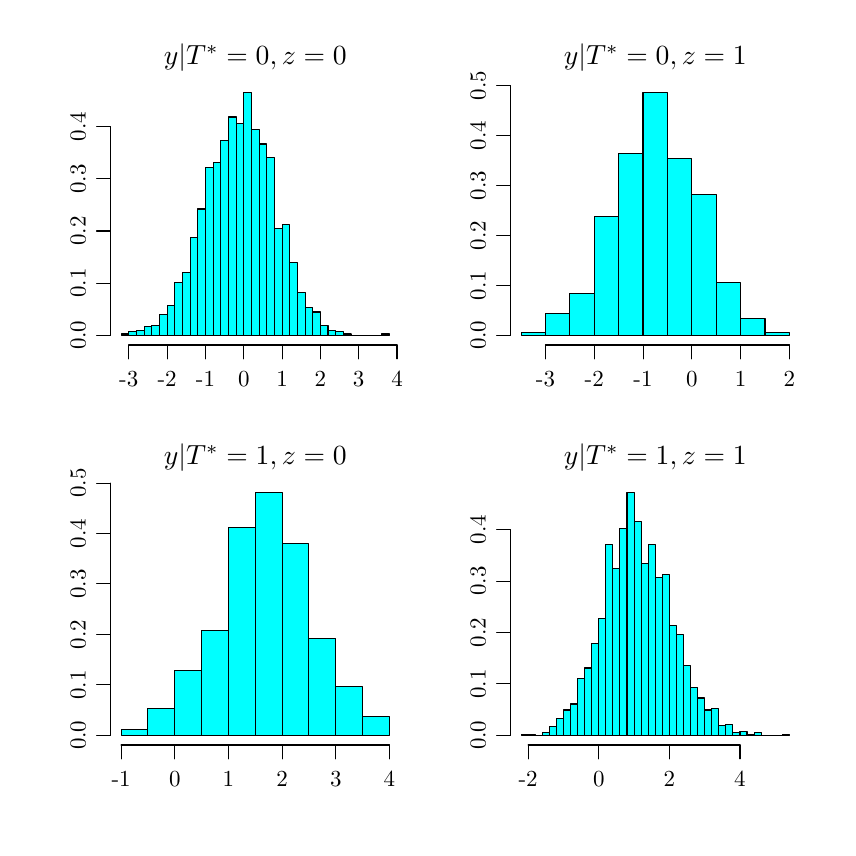
\begin{tikzpicture}[x=1pt,y=1pt]
\definecolor{fillColor}{RGB}{255,255,255}
\path[use as bounding box,fill=fillColor,fill opacity=0.00] (0,0) rectangle (289.08,289.08);
\begin{scope}
\path[clip] (  0.00,  0.00) rectangle (289.08,289.08);
\definecolor{drawColor}{RGB}{0,0,0}

\path[draw=drawColor,line width= 0.4pt,line join=round,line cap=round] ( 36.53,174.42) -- (133.47,174.42);

\path[draw=drawColor,line width= 0.4pt,line join=round,line cap=round] ( 36.53,174.42) -- ( 36.53,169.44);

\path[draw=drawColor,line width= 0.4pt,line join=round,line cap=round] ( 50.38,174.42) -- ( 50.38,169.44);

\path[draw=drawColor,line width= 0.4pt,line join=round,line cap=round] ( 64.23,174.42) -- ( 64.23,169.44);

\path[draw=drawColor,line width= 0.4pt,line join=round,line cap=round] ( 78.08,174.42) -- ( 78.08,169.44);

\path[draw=drawColor,line width= 0.4pt,line join=round,line cap=round] ( 91.93,174.42) -- ( 91.93,169.44);

\path[draw=drawColor,line width= 0.4pt,line join=round,line cap=round] (105.78,174.42) -- (105.78,169.44);

\path[draw=drawColor,line width= 0.4pt,line join=round,line cap=round] (119.63,174.42) -- (119.63,169.44);

\path[draw=drawColor,line width= 0.4pt,line join=round,line cap=round] (133.47,174.42) -- (133.47,169.44);

\node[text=drawColor,anchor=base,inner sep=0pt, outer sep=0pt, scale=  0.83] at ( 36.53,159.48) {-3};

\node[text=drawColor,anchor=base,inner sep=0pt, outer sep=0pt, scale=  0.83] at ( 50.38,159.48) {-2};

\node[text=drawColor,anchor=base,inner sep=0pt, outer sep=0pt, scale=  0.83] at ( 64.23,159.48) {-1};

\node[text=drawColor,anchor=base,inner sep=0pt, outer sep=0pt, scale=  0.83] at ( 78.08,159.48) {0};

\node[text=drawColor,anchor=base,inner sep=0pt, outer sep=0pt, scale=  0.83] at ( 91.93,159.48) {1};

\node[text=drawColor,anchor=base,inner sep=0pt, outer sep=0pt, scale=  0.83] at (105.78,159.48) {2};

\node[text=drawColor,anchor=base,inner sep=0pt, outer sep=0pt, scale=  0.83] at (119.63,159.48) {3};

\node[text=drawColor,anchor=base,inner sep=0pt, outer sep=0pt, scale=  0.83] at (133.47,159.48) {4};

\path[draw=drawColor,line width= 0.4pt,line join=round,line cap=round] ( 29.88,177.93) -- ( 29.88,253.28);

\path[draw=drawColor,line width= 0.4pt,line join=round,line cap=round] ( 29.88,177.93) -- ( 24.90,177.93);

\path[draw=drawColor,line width= 0.4pt,line join=round,line cap=round] ( 29.88,196.77) -- ( 24.90,196.77);

\path[draw=drawColor,line width= 0.4pt,line join=round,line cap=round] ( 29.88,215.61) -- ( 24.90,215.61);

\path[draw=drawColor,line width= 0.4pt,line join=round,line cap=round] ( 29.88,234.44) -- ( 24.90,234.44);

\path[draw=drawColor,line width= 0.4pt,line join=round,line cap=round] ( 29.88,253.28) -- ( 24.90,253.28);

\node[text=drawColor,rotate= 90.00,anchor=base,inner sep=0pt, outer sep=0pt, scale=  0.83] at ( 20.92,177.93) {0.0};

\node[text=drawColor,rotate= 90.00,anchor=base,inner sep=0pt, outer sep=0pt, scale=  0.83] at ( 20.92,196.77) {0.1};

\node[text=drawColor,rotate= 90.00,anchor=base,inner sep=0pt, outer sep=0pt, scale=  0.83] at ( 20.92,215.61) {0.2};

\node[text=drawColor,rotate= 90.00,anchor=base,inner sep=0pt, outer sep=0pt, scale=  0.83] at ( 20.92,234.44) {0.3};

\node[text=drawColor,rotate= 90.00,anchor=base,inner sep=0pt, outer sep=0pt, scale=  0.83] at ( 20.92,253.28) {0.4};
\end{scope}
\begin{scope}
\path[clip] (  0.00,144.54) rectangle (144.54,289.08);
\definecolor{drawColor}{RGB}{0,0,0}

\node[text=drawColor,anchor=base,inner sep=0pt, outer sep=0pt, scale=  1.00] at ( 82.23,275.68) {\bfseries $y|T^*=0,z=0$};
\end{scope}
\begin{scope}
\path[clip] ( 29.88,174.42) rectangle (134.58,269.16);
\definecolor{drawColor}{RGB}{0,0,0}
\definecolor{fillColor}{RGB}{0,255,255}

\path[draw=drawColor,line width= 0.4pt,line join=round,line cap=round,fill=fillColor] ( 33.76,177.93) rectangle ( 36.53,178.37);

\path[draw=drawColor,line width= 0.4pt,line join=round,line cap=round,fill=fillColor] ( 36.53,177.93) rectangle ( 39.30,179.26);

\path[draw=drawColor,line width= 0.4pt,line join=round,line cap=round,fill=fillColor] ( 39.30,177.93) rectangle ( 42.07,179.70);

\path[draw=drawColor,line width= 0.4pt,line join=round,line cap=round,fill=fillColor] ( 42.07,177.93) rectangle ( 44.84,181.03);

\path[draw=drawColor,line width= 0.4pt,line join=round,line cap=round,fill=fillColor] ( 44.84,177.93) rectangle ( 47.61,181.47);

\path[draw=drawColor,line width= 0.4pt,line join=round,line cap=round,fill=fillColor] ( 47.61,177.93) rectangle ( 50.38,185.46);

\path[draw=drawColor,line width= 0.4pt,line join=round,line cap=round,fill=fillColor] ( 50.38,177.93) rectangle ( 53.15,188.56);

\path[draw=drawColor,line width= 0.4pt,line join=round,line cap=round,fill=fillColor] ( 53.15,177.93) rectangle ( 55.92,196.98);

\path[draw=drawColor,line width= 0.4pt,line join=round,line cap=round,fill=fillColor] ( 55.92,177.93) rectangle ( 58.69,200.52);

\path[draw=drawColor,line width= 0.4pt,line join=round,line cap=round,fill=fillColor] ( 58.69,177.93) rectangle ( 61.46,213.37);

\path[draw=drawColor,line width= 0.4pt,line join=round,line cap=round,fill=fillColor] ( 61.46,177.93) rectangle ( 64.23,223.56);

\path[draw=drawColor,line width= 0.4pt,line join=round,line cap=round,fill=fillColor] ( 64.23,177.93) rectangle ( 67.00,238.63);

\path[draw=drawColor,line width= 0.4pt,line join=round,line cap=round,fill=fillColor] ( 67.00,177.93) rectangle ( 69.77,240.40);

\path[draw=drawColor,line width= 0.4pt,line join=round,line cap=round,fill=fillColor] ( 69.77,177.93) rectangle ( 72.54,248.37);

\path[draw=drawColor,line width= 0.4pt,line join=round,line cap=round,fill=fillColor] ( 72.54,177.93) rectangle ( 75.31,256.79);

\path[draw=drawColor,line width= 0.4pt,line join=round,line cap=round,fill=fillColor] ( 75.31,177.93) rectangle ( 78.08,254.58);

\path[draw=drawColor,line width= 0.4pt,line join=round,line cap=round,fill=fillColor] ( 78.08,177.93) rectangle ( 80.85,265.65);

\path[draw=drawColor,line width= 0.4pt,line join=round,line cap=round,fill=fillColor] ( 80.85,177.93) rectangle ( 83.61,252.36);

\path[draw=drawColor,line width= 0.4pt,line join=round,line cap=round,fill=fillColor] ( 83.61,177.93) rectangle ( 86.38,247.04);

\path[draw=drawColor,line width= 0.4pt,line join=round,line cap=round,fill=fillColor] ( 86.38,177.93) rectangle ( 89.15,242.17);

\path[draw=drawColor,line width= 0.4pt,line join=round,line cap=round,fill=fillColor] ( 89.15,177.93) rectangle ( 91.92,216.47);

\path[draw=drawColor,line width= 0.4pt,line join=round,line cap=round,fill=fillColor] ( 91.92,177.93) rectangle ( 94.69,217.80);

\path[draw=drawColor,line width= 0.4pt,line join=round,line cap=round,fill=fillColor] ( 94.69,177.93) rectangle ( 97.46,204.07);

\path[draw=drawColor,line width= 0.4pt,line join=round,line cap=round,fill=fillColor] ( 97.46,177.93) rectangle (100.23,193.44);

\path[draw=drawColor,line width= 0.4pt,line join=round,line cap=round,fill=fillColor] (100.23,177.93) rectangle (103.00,188.12);

\path[draw=drawColor,line width= 0.4pt,line join=round,line cap=round,fill=fillColor] (103.00,177.93) rectangle (105.77,186.35);

\path[draw=drawColor,line width= 0.4pt,line join=round,line cap=round,fill=fillColor] (105.77,177.93) rectangle (108.54,181.47);

\path[draw=drawColor,line width= 0.4pt,line join=round,line cap=round,fill=fillColor] (108.54,177.93) rectangle (111.31,179.70);

\path[draw=drawColor,line width= 0.4pt,line join=round,line cap=round,fill=fillColor] (111.31,177.93) rectangle (114.08,179.26);

\path[draw=drawColor,line width= 0.4pt,line join=round,line cap=round,fill=fillColor] (114.08,177.93) rectangle (116.85,178.37);

\path[draw=drawColor,line width= 0.4pt,line join=round,line cap=round,fill=fillColor] (116.85,177.93) rectangle (119.62,177.93);

\path[draw=drawColor,line width= 0.4pt,line join=round,line cap=round,fill=fillColor] (119.62,177.93) rectangle (122.39,177.93);

\path[draw=drawColor,line width= 0.4pt,line join=round,line cap=round,fill=fillColor] (122.39,177.93) rectangle (125.16,177.93);

\path[draw=drawColor,line width= 0.4pt,line join=round,line cap=round,fill=fillColor] (125.16,177.93) rectangle (127.93,177.93);

\path[draw=drawColor,line width= 0.4pt,line join=round,line cap=round,fill=fillColor] (127.93,177.93) rectangle (130.70,178.37);
\end{scope}
\begin{scope}
\path[clip] (  0.00,  0.00) rectangle (289.08,289.08);
\definecolor{drawColor}{RGB}{0,0,0}

\path[draw=drawColor,line width= 0.4pt,line join=round,line cap=round] (187.12,174.42) -- (275.25,174.42);

\path[draw=drawColor,line width= 0.4pt,line join=round,line cap=round] (187.12,174.42) -- (187.12,169.44);

\path[draw=drawColor,line width= 0.4pt,line join=round,line cap=round] (204.75,174.42) -- (204.75,169.44);

\path[draw=drawColor,line width= 0.4pt,line join=round,line cap=round] (222.37,174.42) -- (222.37,169.44);

\path[draw=drawColor,line width= 0.4pt,line join=round,line cap=round] (240.00,174.42) -- (240.00,169.44);

\path[draw=drawColor,line width= 0.4pt,line join=round,line cap=round] (257.62,174.42) -- (257.62,169.44);

\path[draw=drawColor,line width= 0.4pt,line join=round,line cap=round] (275.25,174.42) -- (275.25,169.44);

\node[text=drawColor,anchor=base,inner sep=0pt, outer sep=0pt, scale=  0.83] at (187.12,159.48) {-3};

\node[text=drawColor,anchor=base,inner sep=0pt, outer sep=0pt, scale=  0.83] at (204.75,159.48) {-2};

\node[text=drawColor,anchor=base,inner sep=0pt, outer sep=0pt, scale=  0.83] at (222.37,159.48) {-1};

\node[text=drawColor,anchor=base,inner sep=0pt, outer sep=0pt, scale=  0.83] at (240.00,159.48) {0};

\node[text=drawColor,anchor=base,inner sep=0pt, outer sep=0pt, scale=  0.83] at (257.62,159.48) {1};

\node[text=drawColor,anchor=base,inner sep=0pt, outer sep=0pt, scale=  0.83] at (275.25,159.48) {2};

\path[draw=drawColor,line width= 0.4pt,line join=round,line cap=round] (174.42,177.93) -- (174.42,268.14);

\path[draw=drawColor,line width= 0.4pt,line join=round,line cap=round] (174.42,177.93) -- (169.44,177.93);

\path[draw=drawColor,line width= 0.4pt,line join=round,line cap=round] (174.42,195.97) -- (169.44,195.97);

\path[draw=drawColor,line width= 0.4pt,line join=round,line cap=round] (174.42,214.01) -- (169.44,214.01);

\path[draw=drawColor,line width= 0.4pt,line join=round,line cap=round] (174.42,232.06) -- (169.44,232.06);

\path[draw=drawColor,line width= 0.4pt,line join=round,line cap=round] (174.42,250.10) -- (169.44,250.10);

\path[draw=drawColor,line width= 0.4pt,line join=round,line cap=round] (174.42,268.14) -- (169.44,268.14);

\node[text=drawColor,rotate= 90.00,anchor=base,inner sep=0pt, outer sep=0pt, scale=  0.83] at (165.46,177.93) {0.0};

\node[text=drawColor,rotate= 90.00,anchor=base,inner sep=0pt, outer sep=0pt, scale=  0.83] at (165.46,195.97) {0.1};

\node[text=drawColor,rotate= 90.00,anchor=base,inner sep=0pt, outer sep=0pt, scale=  0.83] at (165.46,214.01) {0.2};

\node[text=drawColor,rotate= 90.00,anchor=base,inner sep=0pt, outer sep=0pt, scale=  0.83] at (165.46,232.06) {0.3};

\node[text=drawColor,rotate= 90.00,anchor=base,inner sep=0pt, outer sep=0pt, scale=  0.83] at (165.46,250.10) {0.4};

\node[text=drawColor,rotate= 90.00,anchor=base,inner sep=0pt, outer sep=0pt, scale=  0.83] at (165.46,268.14) {0.5};
\end{scope}
\begin{scope}
\path[clip] (144.54,144.54) rectangle (289.08,289.08);
\definecolor{drawColor}{RGB}{0,0,0}

\node[text=drawColor,anchor=base,inner sep=0pt, outer sep=0pt, scale=  1.00] at (226.77,275.68) {\bfseries $y|T^*=0,z=1$};
\end{scope}
\begin{scope}
\path[clip] (174.42,174.42) rectangle (279.12,269.16);
\definecolor{drawColor}{RGB}{0,0,0}
\definecolor{fillColor}{RGB}{0,255,255}

\path[draw=drawColor,line width= 0.4pt,line join=round,line cap=round,fill=fillColor] (178.30,177.93) rectangle (187.11,178.93);

\path[draw=drawColor,line width= 0.4pt,line join=round,line cap=round,fill=fillColor] (187.11,177.93) rectangle (195.92,185.90);

\path[draw=drawColor,line width= 0.4pt,line join=round,line cap=round,fill=fillColor] (195.92,177.93) rectangle (204.74,192.88);

\path[draw=drawColor,line width= 0.4pt,line join=round,line cap=round,fill=fillColor] (204.74,177.93) rectangle (213.55,220.79);

\path[draw=drawColor,line width= 0.4pt,line join=round,line cap=round,fill=fillColor] (213.55,177.93) rectangle (222.36,243.72);

\path[draw=drawColor,line width= 0.4pt,line join=round,line cap=round,fill=fillColor] (222.36,177.93) rectangle (231.18,265.65);

\path[draw=drawColor,line width= 0.4pt,line join=round,line cap=round,fill=fillColor] (231.18,177.93) rectangle (239.99,241.73);

\path[draw=drawColor,line width= 0.4pt,line join=round,line cap=round,fill=fillColor] (239.99,177.93) rectangle (248.80,228.77);

\path[draw=drawColor,line width= 0.4pt,line join=round,line cap=round,fill=fillColor] (248.80,177.93) rectangle (257.62,196.87);

\path[draw=drawColor,line width= 0.4pt,line join=round,line cap=round,fill=fillColor] (257.62,177.93) rectangle (266.43,183.91);

\path[draw=drawColor,line width= 0.4pt,line join=round,line cap=round,fill=fillColor] (266.43,177.93) rectangle (275.24,178.93);
\end{scope}
\begin{scope}
\path[clip] (  0.00,  0.00) rectangle (289.08,289.08);
\definecolor{drawColor}{RGB}{0,0,0}

\path[draw=drawColor,line width= 0.4pt,line join=round,line cap=round] ( 33.77, 29.88) -- (130.71, 29.88);

\path[draw=drawColor,line width= 0.4pt,line join=round,line cap=round] ( 33.77, 29.88) -- ( 33.77, 24.90);

\path[draw=drawColor,line width= 0.4pt,line join=round,line cap=round] ( 53.16, 29.88) -- ( 53.16, 24.90);

\path[draw=drawColor,line width= 0.4pt,line join=round,line cap=round] ( 72.55, 29.88) -- ( 72.55, 24.90);

\path[draw=drawColor,line width= 0.4pt,line join=round,line cap=round] ( 91.93, 29.88) -- ( 91.93, 24.90);

\path[draw=drawColor,line width= 0.4pt,line join=round,line cap=round] (111.32, 29.88) -- (111.32, 24.90);

\path[draw=drawColor,line width= 0.4pt,line join=round,line cap=round] (130.71, 29.88) -- (130.71, 24.90);

\node[text=drawColor,anchor=base,inner sep=0pt, outer sep=0pt, scale=  0.83] at ( 33.77, 14.94) {-1};

\node[text=drawColor,anchor=base,inner sep=0pt, outer sep=0pt, scale=  0.83] at ( 53.16, 14.94) {0};

\node[text=drawColor,anchor=base,inner sep=0pt, outer sep=0pt, scale=  0.83] at ( 72.55, 14.94) {1};

\node[text=drawColor,anchor=base,inner sep=0pt, outer sep=0pt, scale=  0.83] at ( 91.93, 14.94) {2};

\node[text=drawColor,anchor=base,inner sep=0pt, outer sep=0pt, scale=  0.83] at (111.32, 14.94) {3};

\node[text=drawColor,anchor=base,inner sep=0pt, outer sep=0pt, scale=  0.83] at (130.71, 14.94) {4};

\path[draw=drawColor,line width= 0.4pt,line join=round,line cap=round] ( 29.88, 33.39) -- ( 29.88,124.52);

\path[draw=drawColor,line width= 0.4pt,line join=round,line cap=round] ( 29.88, 33.39) -- ( 24.90, 33.39);

\path[draw=drawColor,line width= 0.4pt,line join=round,line cap=round] ( 29.88, 51.62) -- ( 24.90, 51.62);

\path[draw=drawColor,line width= 0.4pt,line join=round,line cap=round] ( 29.88, 69.84) -- ( 24.90, 69.84);

\path[draw=drawColor,line width= 0.4pt,line join=round,line cap=round] ( 29.88, 88.07) -- ( 24.90, 88.07);

\path[draw=drawColor,line width= 0.4pt,line join=round,line cap=round] ( 29.88,106.30) -- ( 24.90,106.30);

\path[draw=drawColor,line width= 0.4pt,line join=round,line cap=round] ( 29.88,124.52) -- ( 24.90,124.52);

\node[text=drawColor,rotate= 90.00,anchor=base,inner sep=0pt, outer sep=0pt, scale=  0.83] at ( 20.92, 33.39) {0.0};

\node[text=drawColor,rotate= 90.00,anchor=base,inner sep=0pt, outer sep=0pt, scale=  0.83] at ( 20.92, 51.62) {0.1};

\node[text=drawColor,rotate= 90.00,anchor=base,inner sep=0pt, outer sep=0pt, scale=  0.83] at ( 20.92, 69.84) {0.2};

\node[text=drawColor,rotate= 90.00,anchor=base,inner sep=0pt, outer sep=0pt, scale=  0.83] at ( 20.92, 88.07) {0.3};

\node[text=drawColor,rotate= 90.00,anchor=base,inner sep=0pt, outer sep=0pt, scale=  0.83] at ( 20.92,106.30) {0.4};

\node[text=drawColor,rotate= 90.00,anchor=base,inner sep=0pt, outer sep=0pt, scale=  0.83] at ( 20.92,124.52) {0.5};
\end{scope}
\begin{scope}
\path[clip] (  0.00,  0.00) rectangle (144.54,144.54);
\definecolor{drawColor}{RGB}{0,0,0}

\node[text=drawColor,anchor=base,inner sep=0pt, outer sep=0pt, scale=  1.00] at ( 82.23,131.14) {\bfseries $y|T^*=1,z=0$};
\end{scope}
\begin{scope}
\path[clip] ( 29.88, 29.88) rectangle (134.58,124.62);
\definecolor{drawColor}{RGB}{0,0,0}
\definecolor{fillColor}{RGB}{0,255,255}

\path[draw=drawColor,line width= 0.4pt,line join=round,line cap=round,fill=fillColor] ( 33.76, 33.39) rectangle ( 43.45, 35.34);

\path[draw=drawColor,line width= 0.4pt,line join=round,line cap=round,fill=fillColor] ( 43.45, 33.39) rectangle ( 53.15, 43.14);

\path[draw=drawColor,line width= 0.4pt,line join=round,line cap=round,fill=fillColor] ( 53.15, 33.39) rectangle ( 62.84, 56.78);

\path[draw=drawColor,line width= 0.4pt,line join=round,line cap=round,fill=fillColor] ( 62.84, 33.39) rectangle ( 72.54, 71.40);

\path[draw=drawColor,line width= 0.4pt,line join=round,line cap=round,fill=fillColor] ( 72.54, 33.39) rectangle ( 82.23,108.44);

\path[draw=drawColor,line width= 0.4pt,line join=round,line cap=round,fill=fillColor] ( 82.23, 33.39) rectangle ( 91.92,121.11);

\path[draw=drawColor,line width= 0.4pt,line join=round,line cap=round,fill=fillColor] ( 91.92, 33.39) rectangle (101.62,102.59);

\path[draw=drawColor,line width= 0.4pt,line join=round,line cap=round,fill=fillColor] (101.62, 33.39) rectangle (111.31, 68.48);

\path[draw=drawColor,line width= 0.4pt,line join=round,line cap=round,fill=fillColor] (111.31, 33.39) rectangle (121.01, 50.93);

\path[draw=drawColor,line width= 0.4pt,line join=round,line cap=round,fill=fillColor] (121.01, 33.39) rectangle (130.70, 40.21);
\end{scope}
\begin{scope}
\path[clip] (  0.00,  0.00) rectangle (289.08,289.08);
\definecolor{drawColor}{RGB}{0,0,0}

\path[draw=drawColor,line width= 0.4pt,line join=round,line cap=round] (180.85, 29.88) -- (257.39, 29.88);

\path[draw=drawColor,line width= 0.4pt,line join=round,line cap=round] (180.85, 29.88) -- (180.85, 24.90);

\path[draw=drawColor,line width= 0.4pt,line join=round,line cap=round] (206.36, 29.88) -- (206.36, 24.90);

\path[draw=drawColor,line width= 0.4pt,line join=round,line cap=round] (231.87, 29.88) -- (231.87, 24.90);

\path[draw=drawColor,line width= 0.4pt,line join=round,line cap=round] (257.39, 29.88) -- (257.39, 24.90);

\node[text=drawColor,anchor=base,inner sep=0pt, outer sep=0pt, scale=  0.83] at (180.85, 14.94) {-2};

\node[text=drawColor,anchor=base,inner sep=0pt, outer sep=0pt, scale=  0.83] at (206.36, 14.94) {0};

\node[text=drawColor,anchor=base,inner sep=0pt, outer sep=0pt, scale=  0.83] at (231.87, 14.94) {2};

\node[text=drawColor,anchor=base,inner sep=0pt, outer sep=0pt, scale=  0.83] at (257.39, 14.94) {4};

\path[draw=drawColor,line width= 0.4pt,line join=round,line cap=round] (174.42, 33.39) -- (174.42,107.67);

\path[draw=drawColor,line width= 0.4pt,line join=round,line cap=round] (174.42, 33.39) -- (169.44, 33.39);

\path[draw=drawColor,line width= 0.4pt,line join=round,line cap=round] (174.42, 51.96) -- (169.44, 51.96);

\path[draw=drawColor,line width= 0.4pt,line join=round,line cap=round] (174.42, 70.53) -- (169.44, 70.53);

\path[draw=drawColor,line width= 0.4pt,line join=round,line cap=round] (174.42, 89.10) -- (169.44, 89.10);

\path[draw=drawColor,line width= 0.4pt,line join=round,line cap=round] (174.42,107.67) -- (169.44,107.67);

\node[text=drawColor,rotate= 90.00,anchor=base,inner sep=0pt, outer sep=0pt, scale=  0.83] at (165.46, 33.39) {0.0};

\node[text=drawColor,rotate= 90.00,anchor=base,inner sep=0pt, outer sep=0pt, scale=  0.83] at (165.46, 51.96) {0.1};

\node[text=drawColor,rotate= 90.00,anchor=base,inner sep=0pt, outer sep=0pt, scale=  0.83] at (165.46, 70.53) {0.2};

\node[text=drawColor,rotate= 90.00,anchor=base,inner sep=0pt, outer sep=0pt, scale=  0.83] at (165.46, 89.10) {0.3};

\node[text=drawColor,rotate= 90.00,anchor=base,inner sep=0pt, outer sep=0pt, scale=  0.83] at (165.46,107.67) {0.4};
\end{scope}
\begin{scope}
\path[clip] (144.54,  0.00) rectangle (289.08,144.54);
\definecolor{drawColor}{RGB}{0,0,0}

\node[text=drawColor,anchor=base,inner sep=0pt, outer sep=0pt, scale=  1.00] at (226.77,131.14) {\bfseries $y|T^*=1,z=1$};
\end{scope}
\begin{scope}
\path[clip] (174.42, 29.88) rectangle (279.12,124.62);
\definecolor{drawColor}{RGB}{0,0,0}
\definecolor{fillColor}{RGB}{0,255,255}

\path[draw=drawColor,line width= 0.4pt,line join=round,line cap=round,fill=fillColor] (178.30, 33.39) rectangle (180.85, 33.82);

\path[draw=drawColor,line width= 0.4pt,line join=round,line cap=round,fill=fillColor] (180.85, 33.39) rectangle (183.40, 33.82);

\path[draw=drawColor,line width= 0.4pt,line join=round,line cap=round,fill=fillColor] (183.40, 33.39) rectangle (185.95, 33.39);

\path[draw=drawColor,line width= 0.4pt,line join=round,line cap=round,fill=fillColor] (185.95, 33.39) rectangle (188.50, 34.26);

\path[draw=drawColor,line width= 0.4pt,line join=round,line cap=round,fill=fillColor] (188.50, 33.39) rectangle (191.05, 36.43);

\path[draw=drawColor,line width= 0.4pt,line join=round,line cap=round,fill=fillColor] (191.05, 33.39) rectangle (193.60, 39.47);

\path[draw=drawColor,line width= 0.4pt,line join=round,line cap=round,fill=fillColor] (193.60, 33.39) rectangle (196.16, 42.51);

\path[draw=drawColor,line width= 0.4pt,line join=round,line cap=round,fill=fillColor] (196.16, 33.39) rectangle (198.71, 44.68);

\path[draw=drawColor,line width= 0.4pt,line join=round,line cap=round,fill=fillColor] (198.71, 33.39) rectangle (201.26, 53.80);

\path[draw=drawColor,line width= 0.4pt,line join=round,line cap=round,fill=fillColor] (201.26, 33.39) rectangle (203.81, 57.71);

\path[draw=drawColor,line width= 0.4pt,line join=round,line cap=round,fill=fillColor] (203.81, 33.39) rectangle (206.36, 66.39);

\path[draw=drawColor,line width= 0.4pt,line join=round,line cap=round,fill=fillColor] (206.36, 33.39) rectangle (208.91, 75.51);

\path[draw=drawColor,line width= 0.4pt,line join=round,line cap=round,fill=fillColor] (208.91, 33.39) rectangle (211.46,102.44);

\path[draw=drawColor,line width= 0.4pt,line join=round,line cap=round,fill=fillColor] (211.46, 33.39) rectangle (214.01, 93.75);

\path[draw=drawColor,line width= 0.4pt,line join=round,line cap=round,fill=fillColor] (214.01, 33.39) rectangle (216.57,108.08);

\path[draw=drawColor,line width= 0.4pt,line join=round,line cap=round,fill=fillColor] (216.57, 33.39) rectangle (219.12,121.11);

\path[draw=drawColor,line width= 0.4pt,line join=round,line cap=round,fill=fillColor] (219.12, 33.39) rectangle (221.67,110.69);

\path[draw=drawColor,line width= 0.4pt,line join=round,line cap=round,fill=fillColor] (221.67, 33.39) rectangle (224.22, 95.49);

\path[draw=drawColor,line width= 0.4pt,line join=round,line cap=round,fill=fillColor] (224.22, 33.39) rectangle (226.77,102.44);

\path[draw=drawColor,line width= 0.4pt,line join=round,line cap=round,fill=fillColor] (226.77, 33.39) rectangle (229.32, 90.28);

\path[draw=drawColor,line width= 0.4pt,line join=round,line cap=round,fill=fillColor] (229.32, 33.39) rectangle (231.87, 91.58);

\path[draw=drawColor,line width= 0.4pt,line join=round,line cap=round,fill=fillColor] (231.87, 33.39) rectangle (234.42, 72.91);

\path[draw=drawColor,line width= 0.4pt,line join=round,line cap=round,fill=fillColor] (234.42, 33.39) rectangle (236.97, 69.87);

\path[draw=drawColor,line width= 0.4pt,line join=round,line cap=round,fill=fillColor] (236.97, 33.39) rectangle (239.53, 58.58);

\path[draw=drawColor,line width= 0.4pt,line join=round,line cap=round,fill=fillColor] (239.53, 33.39) rectangle (242.08, 50.76);

\path[draw=drawColor,line width= 0.4pt,line join=round,line cap=round,fill=fillColor] (242.08, 33.39) rectangle (244.63, 46.85);

\path[draw=drawColor,line width= 0.4pt,line join=round,line cap=round,fill=fillColor] (244.63, 33.39) rectangle (247.18, 42.51);

\path[draw=drawColor,line width= 0.4pt,line join=round,line cap=round,fill=fillColor] (247.18, 33.39) rectangle (249.73, 42.94);

\path[draw=drawColor,line width= 0.4pt,line join=round,line cap=round,fill=fillColor] (249.73, 33.39) rectangle (252.28, 36.86);

\path[draw=drawColor,line width= 0.4pt,line join=round,line cap=round,fill=fillColor] (252.28, 33.39) rectangle (254.83, 37.30);

\path[draw=drawColor,line width= 0.4pt,line join=round,line cap=round,fill=fillColor] (254.83, 33.39) rectangle (257.38, 34.26);

\path[draw=drawColor,line width= 0.4pt,line join=round,line cap=round,fill=fillColor] (257.38, 33.39) rectangle (259.94, 34.69);

\path[draw=drawColor,line width= 0.4pt,line join=round,line cap=round,fill=fillColor] (259.94, 33.39) rectangle (262.49, 33.82);

\path[draw=drawColor,line width= 0.4pt,line join=round,line cap=round,fill=fillColor] (262.49, 33.39) rectangle (265.04, 34.26);

\path[draw=drawColor,line width= 0.4pt,line join=round,line cap=round,fill=fillColor] (265.04, 33.39) rectangle (267.59, 33.39);

\path[draw=drawColor,line width= 0.4pt,line join=round,line cap=round,fill=fillColor] (267.59, 33.39) rectangle (270.14, 33.39);

\path[draw=drawColor,line width= 0.4pt,line join=round,line cap=round,fill=fillColor] (270.14, 33.39) rectangle (272.69, 33.39);

\path[draw=drawColor,line width= 0.4pt,line join=round,line cap=round,fill=fillColor] (272.69, 33.39) rectangle (275.24, 33.82);
\end{scope}
\end{tikzpicture}

}
\end{figure}
\[\widehat{\beta}_{IV} = 0.96, \quad \mbox{95\% CI } = (0.88, 1.04)\]
\end{block}
\end{frame}
%%%%%%%%%%%%%%%%%%%%%%%%%%%%%%%%%%%%%
\begin{frame}[noframenumbering]
  \frametitle{Simulation Example \hfill \small{($\beta = 1, \alpha_0 = 0.1, \alpha_1 = 0.2, n = 5000$)}}

  \begin{alertblock}{Results using $T$ instead of $T^*$}
\begin{figure}[h]
  \centering
\resizebox{0.5\textwidth}{!}{%
  % Created by tikzDevice version 0.10.1 on 2018-01-16 22:08:40
% !TEX encoding = UTF-8 Unicode
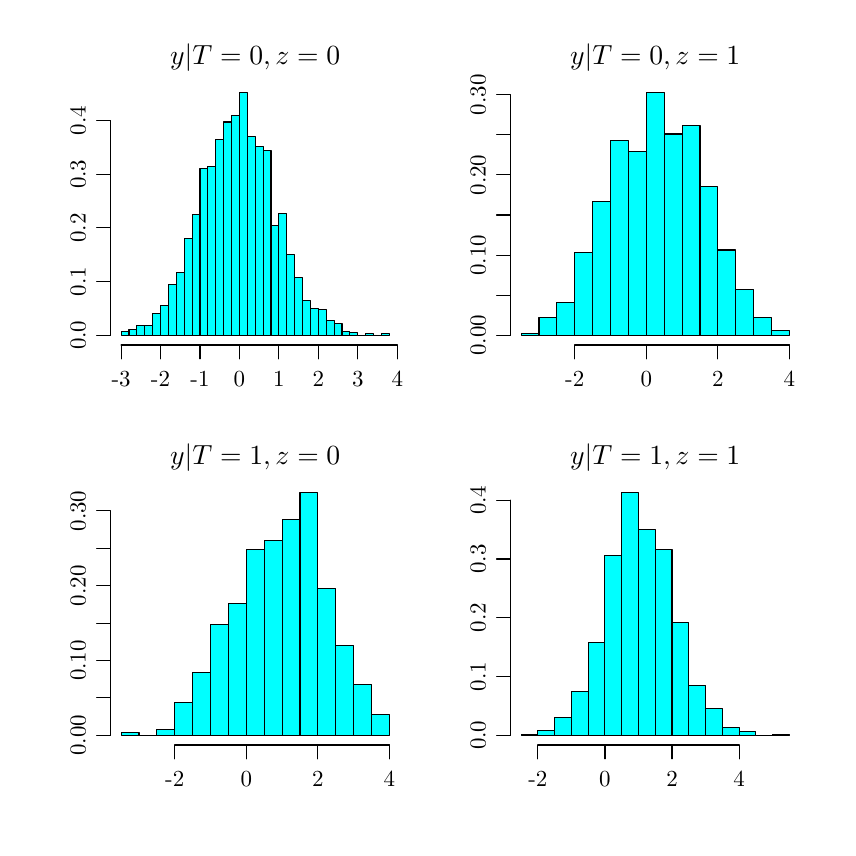
\begin{tikzpicture}[x=1pt,y=1pt]
\definecolor{fillColor}{RGB}{255,255,255}
\path[use as bounding box,fill=fillColor,fill opacity=0.00] (0,0) rectangle (289.08,289.08);
\begin{scope}
\path[clip] (  0.00,  0.00) rectangle (289.08,289.08);
\definecolor{drawColor}{RGB}{0,0,0}

\path[draw=drawColor,line width= 0.4pt,line join=round,line cap=round] ( 33.76,174.42) -- (133.56,174.42);

\path[draw=drawColor,line width= 0.4pt,line join=round,line cap=round] ( 33.76,174.42) -- ( 33.76,169.44);

\path[draw=drawColor,line width= 0.4pt,line join=round,line cap=round] ( 48.02,174.42) -- ( 48.02,169.44);

\path[draw=drawColor,line width= 0.4pt,line join=round,line cap=round] ( 62.27,174.42) -- ( 62.27,169.44);

\path[draw=drawColor,line width= 0.4pt,line join=round,line cap=round] ( 76.53,174.42) -- ( 76.53,169.44);

\path[draw=drawColor,line width= 0.4pt,line join=round,line cap=round] ( 90.79,174.42) -- ( 90.79,169.44);

\path[draw=drawColor,line width= 0.4pt,line join=round,line cap=round] (105.04,174.42) -- (105.04,169.44);

\path[draw=drawColor,line width= 0.4pt,line join=round,line cap=round] (119.30,174.42) -- (119.30,169.44);

\path[draw=drawColor,line width= 0.4pt,line join=round,line cap=round] (133.56,174.42) -- (133.56,169.44);

\node[text=drawColor,anchor=base,inner sep=0pt, outer sep=0pt, scale=  0.83] at ( 33.76,159.48) {-3};

\node[text=drawColor,anchor=base,inner sep=0pt, outer sep=0pt, scale=  0.83] at ( 48.02,159.48) {-2};

\node[text=drawColor,anchor=base,inner sep=0pt, outer sep=0pt, scale=  0.83] at ( 62.27,159.48) {-1};

\node[text=drawColor,anchor=base,inner sep=0pt, outer sep=0pt, scale=  0.83] at ( 76.53,159.48) {0};

\node[text=drawColor,anchor=base,inner sep=0pt, outer sep=0pt, scale=  0.83] at ( 90.79,159.48) {1};

\node[text=drawColor,anchor=base,inner sep=0pt, outer sep=0pt, scale=  0.83] at (105.04,159.48) {2};

\node[text=drawColor,anchor=base,inner sep=0pt, outer sep=0pt, scale=  0.83] at (119.30,159.48) {3};

\node[text=drawColor,anchor=base,inner sep=0pt, outer sep=0pt, scale=  0.83] at (133.56,159.48) {4};

\path[draw=drawColor,line width= 0.4pt,line join=round,line cap=round] ( 29.88,177.93) -- ( 29.88,255.51);

\path[draw=drawColor,line width= 0.4pt,line join=round,line cap=round] ( 29.88,177.93) -- ( 24.90,177.93);

\path[draw=drawColor,line width= 0.4pt,line join=round,line cap=round] ( 29.88,197.32) -- ( 24.90,197.32);

\path[draw=drawColor,line width= 0.4pt,line join=round,line cap=round] ( 29.88,216.72) -- ( 24.90,216.72);

\path[draw=drawColor,line width= 0.4pt,line join=round,line cap=round] ( 29.88,236.12) -- ( 24.90,236.12);

\path[draw=drawColor,line width= 0.4pt,line join=round,line cap=round] ( 29.88,255.51) -- ( 24.90,255.51);

\node[text=drawColor,rotate= 90.00,anchor=base,inner sep=0pt, outer sep=0pt, scale=  0.83] at ( 20.92,177.93) {0.0};

\node[text=drawColor,rotate= 90.00,anchor=base,inner sep=0pt, outer sep=0pt, scale=  0.83] at ( 20.92,197.32) {0.1};

\node[text=drawColor,rotate= 90.00,anchor=base,inner sep=0pt, outer sep=0pt, scale=  0.83] at ( 20.92,216.72) {0.2};

\node[text=drawColor,rotate= 90.00,anchor=base,inner sep=0pt, outer sep=0pt, scale=  0.83] at ( 20.92,236.12) {0.3};

\node[text=drawColor,rotate= 90.00,anchor=base,inner sep=0pt, outer sep=0pt, scale=  0.83] at ( 20.92,255.51) {0.4};
\end{scope}
\begin{scope}
\path[clip] (  0.00,144.54) rectangle (144.54,289.08);
\definecolor{drawColor}{RGB}{0,0,0}

\node[text=drawColor,anchor=base,inner sep=0pt, outer sep=0pt, scale=  1.00] at ( 82.23,275.68) {\bfseries $y|T=0,z=0$};
\end{scope}
\begin{scope}
\path[clip] ( 29.88,174.42) rectangle (134.58,269.16);
\definecolor{drawColor}{RGB}{0,0,0}
\definecolor{fillColor}{RGB}{0,255,255}

\path[draw=drawColor,line width= 0.4pt,line join=round,line cap=round,fill=fillColor] ( 33.76,177.93) rectangle ( 36.61,179.38);

\path[draw=drawColor,line width= 0.4pt,line join=round,line cap=round,fill=fillColor] ( 36.61,177.93) rectangle ( 39.46,179.87);

\path[draw=drawColor,line width= 0.4pt,line join=round,line cap=round,fill=fillColor] ( 39.46,177.93) rectangle ( 42.31,181.32);

\path[draw=drawColor,line width= 0.4pt,line join=round,line cap=round,fill=fillColor] ( 42.31,177.93) rectangle ( 45.16,181.32);

\path[draw=drawColor,line width= 0.4pt,line join=round,line cap=round,fill=fillColor] ( 45.16,177.93) rectangle ( 48.01,185.68);

\path[draw=drawColor,line width= 0.4pt,line join=round,line cap=round,fill=fillColor] ( 48.01,177.93) rectangle ( 50.87,188.59);

\path[draw=drawColor,line width= 0.4pt,line join=round,line cap=round,fill=fillColor] ( 50.87,177.93) rectangle ( 53.72,196.35);

\path[draw=drawColor,line width= 0.4pt,line join=round,line cap=round,fill=fillColor] ( 53.72,177.93) rectangle ( 56.57,200.71);

\path[draw=drawColor,line width= 0.4pt,line join=round,line cap=round,fill=fillColor] ( 56.57,177.93) rectangle ( 59.42,212.82);

\path[draw=drawColor,line width= 0.4pt,line join=round,line cap=round,fill=fillColor] ( 59.42,177.93) rectangle ( 62.27,221.55);

\path[draw=drawColor,line width= 0.4pt,line join=round,line cap=round,fill=fillColor] ( 62.27,177.93) rectangle ( 65.12,238.03);

\path[draw=drawColor,line width= 0.4pt,line join=round,line cap=round,fill=fillColor] ( 65.12,177.93) rectangle ( 67.97,239.00);

\path[draw=drawColor,line width= 0.4pt,line join=round,line cap=round,fill=fillColor] ( 67.97,177.93) rectangle ( 70.82,248.69);

\path[draw=drawColor,line width= 0.4pt,line join=round,line cap=round,fill=fillColor] ( 70.82,177.93) rectangle ( 73.68,254.99);

\path[draw=drawColor,line width= 0.4pt,line join=round,line cap=round,fill=fillColor] ( 73.68,177.93) rectangle ( 76.53,257.41);

\path[draw=drawColor,line width= 0.4pt,line join=round,line cap=round,fill=fillColor] ( 76.53,177.93) rectangle ( 79.38,265.65);

\path[draw=drawColor,line width= 0.4pt,line join=round,line cap=round,fill=fillColor] ( 79.38,177.93) rectangle ( 82.23,249.66);

\path[draw=drawColor,line width= 0.4pt,line join=round,line cap=round,fill=fillColor] ( 82.23,177.93) rectangle ( 85.08,246.26);

\path[draw=drawColor,line width= 0.4pt,line join=round,line cap=round,fill=fillColor] ( 85.08,177.93) rectangle ( 87.93,244.81);

\path[draw=drawColor,line width= 0.4pt,line join=round,line cap=round,fill=fillColor] ( 87.93,177.93) rectangle ( 90.78,217.67);

\path[draw=drawColor,line width= 0.4pt,line join=round,line cap=round,fill=fillColor] ( 90.78,177.93) rectangle ( 93.64,222.03);

\path[draw=drawColor,line width= 0.4pt,line join=round,line cap=round,fill=fillColor] ( 93.64,177.93) rectangle ( 96.49,207.01);

\path[draw=drawColor,line width= 0.4pt,line join=round,line cap=round,fill=fillColor] ( 96.49,177.93) rectangle ( 99.34,198.77);

\path[draw=drawColor,line width= 0.4pt,line join=round,line cap=round,fill=fillColor] ( 99.34,177.93) rectangle (102.19,190.53);

\path[draw=drawColor,line width= 0.4pt,line join=round,line cap=round,fill=fillColor] (102.19,177.93) rectangle (105.04,187.62);

\path[draw=drawColor,line width= 0.4pt,line join=round,line cap=round,fill=fillColor] (105.04,177.93) rectangle (107.89,187.14);

\path[draw=drawColor,line width= 0.4pt,line join=round,line cap=round,fill=fillColor] (107.89,177.93) rectangle (110.74,183.26);

\path[draw=drawColor,line width= 0.4pt,line join=round,line cap=round,fill=fillColor] (110.74,177.93) rectangle (113.59,182.29);

\path[draw=drawColor,line width= 0.4pt,line join=round,line cap=round,fill=fillColor] (113.59,177.93) rectangle (116.45,179.38);

\path[draw=drawColor,line width= 0.4pt,line join=round,line cap=round,fill=fillColor] (116.45,177.93) rectangle (119.30,178.90);

\path[draw=drawColor,line width= 0.4pt,line join=round,line cap=round,fill=fillColor] (119.30,177.93) rectangle (122.15,177.93);

\path[draw=drawColor,line width= 0.4pt,line join=round,line cap=round,fill=fillColor] (122.15,177.93) rectangle (125.00,178.41);

\path[draw=drawColor,line width= 0.4pt,line join=round,line cap=round,fill=fillColor] (125.00,177.93) rectangle (127.85,177.93);

\path[draw=drawColor,line width= 0.4pt,line join=round,line cap=round,fill=fillColor] (127.85,177.93) rectangle (130.70,178.41);
\end{scope}
\begin{scope}
\path[clip] (  0.00,  0.00) rectangle (289.08,289.08);
\definecolor{drawColor}{RGB}{0,0,0}

\path[draw=drawColor,line width= 0.4pt,line join=round,line cap=round] (197.69,174.42) -- (275.25,174.42);

\path[draw=drawColor,line width= 0.4pt,line join=round,line cap=round] (197.69,174.42) -- (197.69,169.44);

\path[draw=drawColor,line width= 0.4pt,line join=round,line cap=round] (223.54,174.42) -- (223.54,169.44);

\path[draw=drawColor,line width= 0.4pt,line join=round,line cap=round] (249.40,174.42) -- (249.40,169.44);

\path[draw=drawColor,line width= 0.4pt,line join=round,line cap=round] (275.25,174.42) -- (275.25,169.44);

\node[text=drawColor,anchor=base,inner sep=0pt, outer sep=0pt, scale=  0.83] at (197.69,159.48) {-2};

\node[text=drawColor,anchor=base,inner sep=0pt, outer sep=0pt, scale=  0.83] at (223.54,159.48) {0};

\node[text=drawColor,anchor=base,inner sep=0pt, outer sep=0pt, scale=  0.83] at (249.40,159.48) {2};

\node[text=drawColor,anchor=base,inner sep=0pt, outer sep=0pt, scale=  0.83] at (275.25,159.48) {4};

\path[draw=drawColor,line width= 0.4pt,line join=round,line cap=round] (174.42,177.93) -- (174.42,264.82);

\path[draw=drawColor,line width= 0.4pt,line join=round,line cap=round] (174.42,177.93) -- (169.44,177.93);

\path[draw=drawColor,line width= 0.4pt,line join=round,line cap=round] (174.42,192.41) -- (169.44,192.41);

\path[draw=drawColor,line width= 0.4pt,line join=round,line cap=round] (174.42,206.89) -- (169.44,206.89);

\path[draw=drawColor,line width= 0.4pt,line join=round,line cap=round] (174.42,221.38) -- (169.44,221.38);

\path[draw=drawColor,line width= 0.4pt,line join=round,line cap=round] (174.42,235.86) -- (169.44,235.86);

\path[draw=drawColor,line width= 0.4pt,line join=round,line cap=round] (174.42,250.34) -- (169.44,250.34);

\path[draw=drawColor,line width= 0.4pt,line join=round,line cap=round] (174.42,264.82) -- (169.44,264.82);

\node[text=drawColor,rotate= 90.00,anchor=base,inner sep=0pt, outer sep=0pt, scale=  0.83] at (165.46,177.93) {0.00};

\node[text=drawColor,rotate= 90.00,anchor=base,inner sep=0pt, outer sep=0pt, scale=  0.83] at (165.46,206.89) {0.10};

\node[text=drawColor,rotate= 90.00,anchor=base,inner sep=0pt, outer sep=0pt, scale=  0.83] at (165.46,235.86) {0.20};

\node[text=drawColor,rotate= 90.00,anchor=base,inner sep=0pt, outer sep=0pt, scale=  0.83] at (165.46,264.82) {0.30};
\end{scope}
\begin{scope}
\path[clip] (144.54,144.54) rectangle (289.08,289.08);
\definecolor{drawColor}{RGB}{0,0,0}

\node[text=drawColor,anchor=base,inner sep=0pt, outer sep=0pt, scale=  1.00] at (226.77,275.68) {\bfseries $y|T=0,z=1$};
\end{scope}
\begin{scope}
\path[clip] (174.42,174.42) rectangle (279.12,269.16);
\definecolor{drawColor}{RGB}{0,0,0}
\definecolor{fillColor}{RGB}{0,255,255}

\path[draw=drawColor,line width= 0.4pt,line join=round,line cap=round,fill=fillColor] (178.30,177.93) rectangle (184.76,178.72);

\path[draw=drawColor,line width= 0.4pt,line join=round,line cap=round,fill=fillColor] (184.76,177.93) rectangle (191.22,184.25);

\path[draw=drawColor,line width= 0.4pt,line join=round,line cap=round,fill=fillColor] (191.22,177.93) rectangle (197.69,189.78);

\path[draw=drawColor,line width= 0.4pt,line join=round,line cap=round,fill=fillColor] (197.69,177.93) rectangle (204.15,207.96);

\path[draw=drawColor,line width= 0.4pt,line join=round,line cap=round,fill=fillColor] (204.15,177.93) rectangle (210.61,226.14);

\path[draw=drawColor,line width= 0.4pt,line join=round,line cap=round,fill=fillColor] (210.61,177.93) rectangle (217.08,248.26);

\path[draw=drawColor,line width= 0.4pt,line join=round,line cap=round,fill=fillColor] (217.08,177.93) rectangle (223.54,244.31);

\path[draw=drawColor,line width= 0.4pt,line join=round,line cap=round,fill=fillColor] (223.54,177.93) rectangle (230.00,265.65);

\path[draw=drawColor,line width= 0.4pt,line join=round,line cap=round,fill=fillColor] (230.00,177.93) rectangle (236.46,250.64);

\path[draw=drawColor,line width= 0.4pt,line join=round,line cap=round,fill=fillColor] (236.46,177.93) rectangle (242.93,253.80);

\path[draw=drawColor,line width= 0.4pt,line join=round,line cap=round,fill=fillColor] (242.93,177.93) rectangle (249.39,231.67);

\path[draw=drawColor,line width= 0.4pt,line join=round,line cap=round,fill=fillColor] (249.39,177.93) rectangle (255.85,208.75);

\path[draw=drawColor,line width= 0.4pt,line join=round,line cap=round,fill=fillColor] (255.85,177.93) rectangle (262.32,194.52);

\path[draw=drawColor,line width= 0.4pt,line join=round,line cap=round,fill=fillColor] (262.32,177.93) rectangle (268.78,184.25);

\path[draw=drawColor,line width= 0.4pt,line join=round,line cap=round,fill=fillColor] (268.78,177.93) rectangle (275.24,179.51);
\end{scope}
\begin{scope}
\path[clip] (  0.00,  0.00) rectangle (289.08,289.08);
\definecolor{drawColor}{RGB}{0,0,0}

\path[draw=drawColor,line width= 0.4pt,line join=round,line cap=round] ( 53.15, 29.88) -- (130.71, 29.88);

\path[draw=drawColor,line width= 0.4pt,line join=round,line cap=round] ( 53.15, 29.88) -- ( 53.15, 24.90);

\path[draw=drawColor,line width= 0.4pt,line join=round,line cap=round] ( 79.00, 29.88) -- ( 79.00, 24.90);

\path[draw=drawColor,line width= 0.4pt,line join=round,line cap=round] (104.86, 29.88) -- (104.86, 24.90);

\path[draw=drawColor,line width= 0.4pt,line join=round,line cap=round] (130.71, 29.88) -- (130.71, 24.90);

\node[text=drawColor,anchor=base,inner sep=0pt, outer sep=0pt, scale=  0.83] at ( 53.15, 14.94) {-2};

\node[text=drawColor,anchor=base,inner sep=0pt, outer sep=0pt, scale=  0.83] at ( 79.00, 14.94) {0};

\node[text=drawColor,anchor=base,inner sep=0pt, outer sep=0pt, scale=  0.83] at (104.86, 14.94) {2};

\node[text=drawColor,anchor=base,inner sep=0pt, outer sep=0pt, scale=  0.83] at (130.71, 14.94) {4};

\path[draw=drawColor,line width= 0.4pt,line join=round,line cap=round] ( 29.88, 33.39) -- ( 29.88,114.45);

\path[draw=drawColor,line width= 0.4pt,line join=round,line cap=round] ( 29.88, 33.39) -- ( 24.90, 33.39);

\path[draw=drawColor,line width= 0.4pt,line join=round,line cap=round] ( 29.88, 46.90) -- ( 24.90, 46.90);

\path[draw=drawColor,line width= 0.4pt,line join=round,line cap=round] ( 29.88, 60.41) -- ( 24.90, 60.41);

\path[draw=drawColor,line width= 0.4pt,line join=round,line cap=round] ( 29.88, 73.92) -- ( 24.90, 73.92);

\path[draw=drawColor,line width= 0.4pt,line join=round,line cap=round] ( 29.88, 87.43) -- ( 24.90, 87.43);

\path[draw=drawColor,line width= 0.4pt,line join=round,line cap=round] ( 29.88,100.94) -- ( 24.90,100.94);

\path[draw=drawColor,line width= 0.4pt,line join=round,line cap=round] ( 29.88,114.45) -- ( 24.90,114.45);

\node[text=drawColor,rotate= 90.00,anchor=base,inner sep=0pt, outer sep=0pt, scale=  0.83] at ( 20.92, 33.39) {0.00};

\node[text=drawColor,rotate= 90.00,anchor=base,inner sep=0pt, outer sep=0pt, scale=  0.83] at ( 20.92, 60.41) {0.10};

\node[text=drawColor,rotate= 90.00,anchor=base,inner sep=0pt, outer sep=0pt, scale=  0.83] at ( 20.92, 87.43) {0.20};

\node[text=drawColor,rotate= 90.00,anchor=base,inner sep=0pt, outer sep=0pt, scale=  0.83] at ( 20.92,114.45) {0.30};
\end{scope}
\begin{scope}
\path[clip] (  0.00,  0.00) rectangle (144.54,144.54);
\definecolor{drawColor}{RGB}{0,0,0}

\node[text=drawColor,anchor=base,inner sep=0pt, outer sep=0pt, scale=  1.00] at ( 82.23,131.14) {\bfseries $y|T=1,z=0$};
\end{scope}
\begin{scope}
\path[clip] ( 29.88, 29.88) rectangle (134.58,124.62);
\definecolor{drawColor}{RGB}{0,0,0}
\definecolor{fillColor}{RGB}{0,255,255}

\path[draw=drawColor,line width= 0.4pt,line join=round,line cap=round,fill=fillColor] ( 33.76, 33.39) rectangle ( 40.22, 34.47);

\path[draw=drawColor,line width= 0.4pt,line join=round,line cap=round,fill=fillColor] ( 40.22, 33.39) rectangle ( 46.68, 33.39);

\path[draw=drawColor,line width= 0.4pt,line join=round,line cap=round,fill=fillColor] ( 46.68, 33.39) rectangle ( 53.15, 35.55);

\path[draw=drawColor,line width= 0.4pt,line join=round,line cap=round,fill=fillColor] ( 53.15, 33.39) rectangle ( 59.61, 45.30);

\path[draw=drawColor,line width= 0.4pt,line join=round,line cap=round,fill=fillColor] ( 59.61, 33.39) rectangle ( 66.07, 56.13);

\path[draw=drawColor,line width= 0.4pt,line join=round,line cap=round,fill=fillColor] ( 66.07, 33.39) rectangle ( 72.54, 73.46);

\path[draw=drawColor,line width= 0.4pt,line join=round,line cap=round,fill=fillColor] ( 72.54, 33.39) rectangle ( 79.00, 81.04);

\path[draw=drawColor,line width= 0.4pt,line join=round,line cap=round,fill=fillColor] ( 79.00, 33.39) rectangle ( 85.46,100.53);

\path[draw=drawColor,line width= 0.4pt,line join=round,line cap=round,fill=fillColor] ( 85.46, 33.39) rectangle ( 91.92,103.78);

\path[draw=drawColor,line width= 0.4pt,line join=round,line cap=round,fill=fillColor] ( 91.92, 33.39) rectangle ( 98.39,111.36);

\path[draw=drawColor,line width= 0.4pt,line join=round,line cap=round,fill=fillColor] ( 98.39, 33.39) rectangle (104.85,121.11);

\path[draw=drawColor,line width= 0.4pt,line join=round,line cap=round,fill=fillColor] (104.85, 33.39) rectangle (111.31, 86.46);

\path[draw=drawColor,line width= 0.4pt,line join=round,line cap=round,fill=fillColor] (111.31, 33.39) rectangle (117.78, 65.88);

\path[draw=drawColor,line width= 0.4pt,line join=round,line cap=round,fill=fillColor] (117.78, 33.39) rectangle (124.24, 51.80);

\path[draw=drawColor,line width= 0.4pt,line join=round,line cap=round,fill=fillColor] (124.24, 33.39) rectangle (130.70, 40.97);
\end{scope}
\begin{scope}
\path[clip] (  0.00,  0.00) rectangle (289.08,289.08);
\definecolor{drawColor}{RGB}{0,0,0}

\path[draw=drawColor,line width= 0.4pt,line join=round,line cap=round] (184.36, 29.88) -- (257.07, 29.88);

\path[draw=drawColor,line width= 0.4pt,line join=round,line cap=round] (184.36, 29.88) -- (184.36, 24.90);

\path[draw=drawColor,line width= 0.4pt,line join=round,line cap=round] (208.60, 29.88) -- (208.60, 24.90);

\path[draw=drawColor,line width= 0.4pt,line join=round,line cap=round] (232.84, 29.88) -- (232.84, 24.90);

\path[draw=drawColor,line width= 0.4pt,line join=round,line cap=round] (257.07, 29.88) -- (257.07, 24.90);

\node[text=drawColor,anchor=base,inner sep=0pt, outer sep=0pt, scale=  0.83] at (184.36, 14.94) {-2};

\node[text=drawColor,anchor=base,inner sep=0pt, outer sep=0pt, scale=  0.83] at (208.60, 14.94) {0};

\node[text=drawColor,anchor=base,inner sep=0pt, outer sep=0pt, scale=  0.83] at (232.84, 14.94) {2};

\node[text=drawColor,anchor=base,inner sep=0pt, outer sep=0pt, scale=  0.83] at (257.07, 14.94) {4};

\path[draw=drawColor,line width= 0.4pt,line join=round,line cap=round] (174.42, 33.39) -- (174.42,118.32);

\path[draw=drawColor,line width= 0.4pt,line join=round,line cap=round] (174.42, 33.39) -- (169.44, 33.39);

\path[draw=drawColor,line width= 0.4pt,line join=round,line cap=round] (174.42, 54.62) -- (169.44, 54.62);

\path[draw=drawColor,line width= 0.4pt,line join=round,line cap=round] (174.42, 75.86) -- (169.44, 75.86);

\path[draw=drawColor,line width= 0.4pt,line join=round,line cap=round] (174.42, 97.09) -- (169.44, 97.09);

\path[draw=drawColor,line width= 0.4pt,line join=round,line cap=round] (174.42,118.32) -- (169.44,118.32);

\node[text=drawColor,rotate= 90.00,anchor=base,inner sep=0pt, outer sep=0pt, scale=  0.83] at (165.46, 33.39) {0.0};

\node[text=drawColor,rotate= 90.00,anchor=base,inner sep=0pt, outer sep=0pt, scale=  0.83] at (165.46, 54.62) {0.1};

\node[text=drawColor,rotate= 90.00,anchor=base,inner sep=0pt, outer sep=0pt, scale=  0.83] at (165.46, 75.86) {0.2};

\node[text=drawColor,rotate= 90.00,anchor=base,inner sep=0pt, outer sep=0pt, scale=  0.83] at (165.46, 97.09) {0.3};

\node[text=drawColor,rotate= 90.00,anchor=base,inner sep=0pt, outer sep=0pt, scale=  0.83] at (165.46,118.32) {0.4};
\end{scope}
\begin{scope}
\path[clip] (144.54,  0.00) rectangle (289.08,144.54);
\definecolor{drawColor}{RGB}{0,0,0}

\node[text=drawColor,anchor=base,inner sep=0pt, outer sep=0pt, scale=  1.00] at (226.77,131.14) {\bfseries $y|T=1,z=1$};
\end{scope}
\begin{scope}
\path[clip] (174.42, 29.88) rectangle (279.12,124.62);
\definecolor{drawColor}{RGB}{0,0,0}
\definecolor{fillColor}{RGB}{0,255,255}

\path[draw=drawColor,line width= 0.4pt,line join=round,line cap=round,fill=fillColor] (178.30, 33.39) rectangle (184.36, 33.63);

\path[draw=drawColor,line width= 0.4pt,line join=round,line cap=round,fill=fillColor] (184.36, 33.39) rectangle (190.42, 35.07);

\path[draw=drawColor,line width= 0.4pt,line join=round,line cap=round,fill=fillColor] (190.42, 33.39) rectangle (196.47, 39.88);

\path[draw=drawColor,line width= 0.4pt,line join=round,line cap=round,fill=fillColor] (196.47, 33.39) rectangle (202.53, 49.25);

\path[draw=drawColor,line width= 0.4pt,line join=round,line cap=round,fill=fillColor] (202.53, 33.39) rectangle (208.59, 66.80);

\path[draw=drawColor,line width= 0.4pt,line join=round,line cap=round,fill=fillColor] (208.59, 33.39) rectangle (214.65, 98.28);

\path[draw=drawColor,line width= 0.4pt,line join=round,line cap=round,fill=fillColor] (214.65, 33.39) rectangle (220.71,121.11);

\path[draw=drawColor,line width= 0.4pt,line join=round,line cap=round,fill=fillColor] (220.71, 33.39) rectangle (226.77,107.65);

\path[draw=drawColor,line width= 0.4pt,line join=round,line cap=round,fill=fillColor] (226.77, 33.39) rectangle (232.83,100.44);

\path[draw=drawColor,line width= 0.4pt,line join=round,line cap=round,fill=fillColor] (232.83, 33.39) rectangle (238.89, 74.25);

\path[draw=drawColor,line width= 0.4pt,line join=round,line cap=round,fill=fillColor] (238.89, 33.39) rectangle (244.95, 51.41);

\path[draw=drawColor,line width= 0.4pt,line join=round,line cap=round,fill=fillColor] (244.95, 33.39) rectangle (251.01, 43.00);

\path[draw=drawColor,line width= 0.4pt,line join=round,line cap=round,fill=fillColor] (251.01, 33.39) rectangle (257.07, 36.27);

\path[draw=drawColor,line width= 0.4pt,line join=round,line cap=round,fill=fillColor] (257.07, 33.39) rectangle (263.12, 34.83);

\path[draw=drawColor,line width= 0.4pt,line join=round,line cap=round,fill=fillColor] (263.12, 33.39) rectangle (269.18, 33.39);

\path[draw=drawColor,line width= 0.4pt,line join=round,line cap=round,fill=fillColor] (269.18, 33.39) rectangle (275.24, 33.63);
\end{scope}
\end{tikzpicture}

}
\end{figure}
\[\alert{\widehat{\beta}_{IV} = 1.34, \quad \mbox{95\% CI } = (1.22, 1.45)}\]
\end{alertblock}
\end{frame}
%%%%%%%%%%%%%%%%%%%%%%%%%%%%%%%%%%%%%
\begin{frame}
  \frametitle{Simulation Example \hfill \small{($\beta = 1, \alpha_0 = 0.1, \alpha_1 = 0.2, n = 5000$)}}

\begin{columns}
  \column{0.6\textwidth}
  \vspace{-2em}
\begin{figure}[h]
  \centering
\resizebox{\textwidth}{!}{%
  % Created by tikzDevice version 0.10.1 on 2018-01-16 22:31:42
% !TEX encoding = UTF-8 Unicode
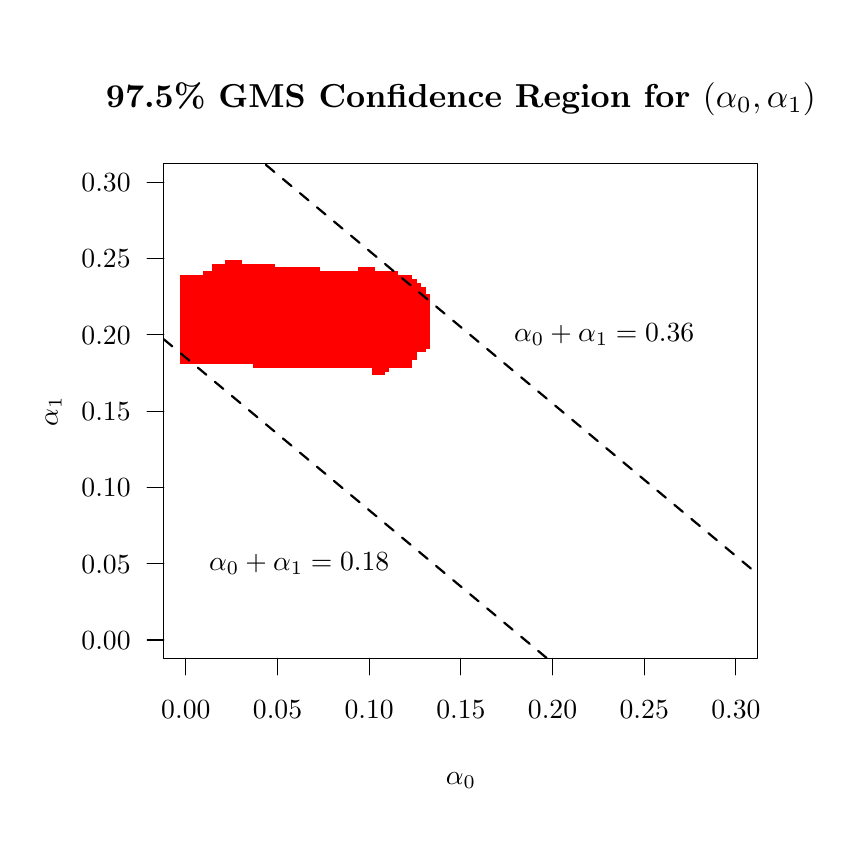
\begin{tikzpicture}[x=1pt,y=1pt]
\definecolor{fillColor}{RGB}{255,255,255}
\path[use as bounding box,fill=fillColor,fill opacity=0.00] (0,0) rectangle (289.08,289.08);
\begin{scope}
\path[clip] ( 49.20, 61.20) rectangle (263.88,239.88);
\definecolor{fillColor}{RGB}{255,0,0}

\path[fill=fillColor] (124.47,163.46) --
	(128.97,163.46) --
	(128.97,167.96) --
	(124.47,167.96) --
	cycle;

\path[fill=fillColor] (124.47,164.83) --
	(128.97,164.83) --
	(128.97,169.33) --
	(124.47,169.33) --
	cycle;

\path[fill=fillColor] (126.13,164.83) --
	(130.63,164.83) --
	(130.63,169.33) --
	(126.13,169.33) --
	cycle;

\path[fill=fillColor] ( 81.40,166.21) --
	( 85.90,166.21) --
	( 85.90,170.71) --
	( 81.40,170.71) --
	cycle;

\path[fill=fillColor] ( 83.06,166.21) --
	( 87.56,166.21) --
	( 87.56,170.71) --
	( 83.06,170.71) --
	cycle;

\path[fill=fillColor] ( 84.72,166.21) --
	( 89.22,166.21) --
	( 89.22,170.71) --
	( 84.72,170.71) --
	cycle;

\path[fill=fillColor] ( 86.37,166.21) --
	( 90.87,166.21) --
	( 90.87,170.71) --
	( 86.37,170.71) --
	cycle;

\path[fill=fillColor] ( 88.03,166.21) --
	( 92.53,166.21) --
	( 92.53,170.71) --
	( 88.03,170.71) --
	cycle;

\path[fill=fillColor] ( 89.69,166.21) --
	( 94.19,166.21) --
	( 94.19,170.71) --
	( 89.69,170.71) --
	cycle;

\path[fill=fillColor] ( 91.34,166.21) --
	( 95.84,166.21) --
	( 95.84,170.71) --
	( 91.34,170.71) --
	cycle;

\path[fill=fillColor] ( 93.00,166.21) --
	( 97.50,166.21) --
	( 97.50,170.71) --
	( 93.00,170.71) --
	cycle;

\path[fill=fillColor] ( 94.66,166.21) --
	( 99.16,166.21) --
	( 99.16,170.71) --
	( 94.66,170.71) --
	cycle;

\path[fill=fillColor] ( 96.31,166.21) --
	(100.81,166.21) --
	(100.81,170.71) --
	( 96.31,170.71) --
	cycle;

\path[fill=fillColor] ( 97.97,166.21) --
	(102.47,166.21) --
	(102.47,170.71) --
	( 97.97,170.71) --
	cycle;

\path[fill=fillColor] ( 99.63,166.21) --
	(104.13,166.21) --
	(104.13,170.71) --
	( 99.63,170.71) --
	cycle;

\path[fill=fillColor] (101.28,166.21) --
	(105.78,166.21) --
	(105.78,170.71) --
	(101.28,170.71) --
	cycle;

\path[fill=fillColor] (102.94,166.21) --
	(107.44,166.21) --
	(107.44,170.71) --
	(102.94,170.71) --
	cycle;

\path[fill=fillColor] (104.60,166.21) --
	(109.10,166.21) --
	(109.10,170.71) --
	(104.60,170.71) --
	cycle;

\path[fill=fillColor] (106.25,166.21) --
	(110.75,166.21) --
	(110.75,170.71) --
	(106.25,170.71) --
	cycle;

\path[fill=fillColor] (107.91,166.21) --
	(112.41,166.21) --
	(112.41,170.71) --
	(107.91,170.71) --
	cycle;

\path[fill=fillColor] (109.56,166.21) --
	(114.06,166.21) --
	(114.06,170.71) --
	(109.56,170.71) --
	cycle;

\path[fill=fillColor] (111.22,166.21) --
	(115.72,166.21) --
	(115.72,170.71) --
	(111.22,170.71) --
	cycle;

\path[fill=fillColor] (114.53,166.21) --
	(119.03,166.21) --
	(119.03,170.71) --
	(114.53,170.71) --
	cycle;

\path[fill=fillColor] (116.19,166.21) --
	(120.69,166.21) --
	(120.69,170.71) --
	(116.19,170.71) --
	cycle;

\path[fill=fillColor] (117.85,166.21) --
	(122.35,166.21) --
	(122.35,170.71) --
	(117.85,170.71) --
	cycle;

\path[fill=fillColor] (119.50,166.21) --
	(124.00,166.21) --
	(124.00,170.71) --
	(119.50,170.71) --
	cycle;

\path[fill=fillColor] (121.16,166.21) --
	(125.66,166.21) --
	(125.66,170.71) --
	(121.16,170.71) --
	cycle;

\path[fill=fillColor] (122.82,166.21) --
	(127.32,166.21) --
	(127.32,170.71) --
	(122.82,170.71) --
	cycle;

\path[fill=fillColor] (124.47,166.21) --
	(128.97,166.21) --
	(128.97,170.71) --
	(124.47,170.71) --
	cycle;

\path[fill=fillColor] (126.13,166.21) --
	(130.63,166.21) --
	(130.63,170.71) --
	(126.13,170.71) --
	cycle;

\path[fill=fillColor] (127.79,166.21) --
	(132.29,166.21) --
	(132.29,170.71) --
	(127.79,170.71) --
	cycle;

\path[fill=fillColor] (129.44,166.21) --
	(133.94,166.21) --
	(133.94,170.71) --
	(129.44,170.71) --
	cycle;

\path[fill=fillColor] (131.10,166.21) --
	(135.60,166.21) --
	(135.60,170.71) --
	(131.10,170.71) --
	cycle;

\path[fill=fillColor] (132.76,166.21) --
	(137.26,166.21) --
	(137.26,170.71) --
	(132.76,170.71) --
	cycle;

\path[fill=fillColor] (134.41,166.21) --
	(138.91,166.21) --
	(138.91,170.71) --
	(134.41,170.71) --
	cycle;

\path[fill=fillColor] ( 54.90,167.59) --
	( 59.40,167.59) --
	( 59.40,172.09) --
	( 54.90,172.09) --
	cycle;

\path[fill=fillColor] ( 56.56,167.59) --
	( 61.06,167.59) --
	( 61.06,172.09) --
	( 56.56,172.09) --
	cycle;

\path[fill=fillColor] ( 58.21,167.59) --
	( 62.71,167.59) --
	( 62.71,172.09) --
	( 58.21,172.09) --
	cycle;

\path[fill=fillColor] ( 59.87,167.59) --
	( 64.37,167.59) --
	( 64.37,172.09) --
	( 59.87,172.09) --
	cycle;

\path[fill=fillColor] ( 61.53,167.59) --
	( 66.03,167.59) --
	( 66.03,172.09) --
	( 61.53,172.09) --
	cycle;

\path[fill=fillColor] ( 63.18,167.59) --
	( 67.68,167.59) --
	( 67.68,172.09) --
	( 63.18,172.09) --
	cycle;

\path[fill=fillColor] ( 64.84,167.59) --
	( 69.34,167.59) --
	( 69.34,172.09) --
	( 64.84,172.09) --
	cycle;

\path[fill=fillColor] ( 66.50,167.59) --
	( 71.00,167.59) --
	( 71.00,172.09) --
	( 66.50,172.09) --
	cycle;

\path[fill=fillColor] ( 68.15,167.59) --
	( 72.65,167.59) --
	( 72.65,172.09) --
	( 68.15,172.09) --
	cycle;

\path[fill=fillColor] ( 69.81,167.59) --
	( 74.31,167.59) --
	( 74.31,172.09) --
	( 69.81,172.09) --
	cycle;

\path[fill=fillColor] ( 71.47,167.59) --
	( 75.97,167.59) --
	( 75.97,172.09) --
	( 71.47,172.09) --
	cycle;

\path[fill=fillColor] ( 73.12,167.59) --
	( 77.62,167.59) --
	( 77.62,172.09) --
	( 73.12,172.09) --
	cycle;

\path[fill=fillColor] ( 74.78,167.59) --
	( 79.28,167.59) --
	( 79.28,172.09) --
	( 74.78,172.09) --
	cycle;

\path[fill=fillColor] ( 76.44,167.59) --
	( 80.94,167.59) --
	( 80.94,172.09) --
	( 76.44,172.09) --
	cycle;

\path[fill=fillColor] ( 78.09,167.59) --
	( 82.59,167.59) --
	( 82.59,172.09) --
	( 78.09,172.09) --
	cycle;

\path[fill=fillColor] ( 79.75,167.59) --
	( 84.25,167.59) --
	( 84.25,172.09) --
	( 79.75,172.09) --
	cycle;

\path[fill=fillColor] ( 81.40,167.59) --
	( 85.90,167.59) --
	( 85.90,172.09) --
	( 81.40,172.09) --
	cycle;

\path[fill=fillColor] ( 83.06,167.59) --
	( 87.56,167.59) --
	( 87.56,172.09) --
	( 83.06,172.09) --
	cycle;

\path[fill=fillColor] ( 84.72,167.59) --
	( 89.22,167.59) --
	( 89.22,172.09) --
	( 84.72,172.09) --
	cycle;

\path[fill=fillColor] ( 86.37,167.59) --
	( 90.87,167.59) --
	( 90.87,172.09) --
	( 86.37,172.09) --
	cycle;

\path[fill=fillColor] ( 88.03,167.59) --
	( 92.53,167.59) --
	( 92.53,172.09) --
	( 88.03,172.09) --
	cycle;

\path[fill=fillColor] ( 89.69,167.59) --
	( 94.19,167.59) --
	( 94.19,172.09) --
	( 89.69,172.09) --
	cycle;

\path[fill=fillColor] ( 91.34,167.59) --
	( 95.84,167.59) --
	( 95.84,172.09) --
	( 91.34,172.09) --
	cycle;

\path[fill=fillColor] ( 93.00,167.59) --
	( 97.50,167.59) --
	( 97.50,172.09) --
	( 93.00,172.09) --
	cycle;

\path[fill=fillColor] ( 94.66,167.59) --
	( 99.16,167.59) --
	( 99.16,172.09) --
	( 94.66,172.09) --
	cycle;

\path[fill=fillColor] ( 96.31,167.59) --
	(100.81,167.59) --
	(100.81,172.09) --
	( 96.31,172.09) --
	cycle;

\path[fill=fillColor] ( 97.97,167.59) --
	(102.47,167.59) --
	(102.47,172.09) --
	( 97.97,172.09) --
	cycle;

\path[fill=fillColor] ( 99.63,167.59) --
	(104.13,167.59) --
	(104.13,172.09) --
	( 99.63,172.09) --
	cycle;

\path[fill=fillColor] (101.28,167.59) --
	(105.78,167.59) --
	(105.78,172.09) --
	(101.28,172.09) --
	cycle;

\path[fill=fillColor] (102.94,167.59) --
	(107.44,167.59) --
	(107.44,172.09) --
	(102.94,172.09) --
	cycle;

\path[fill=fillColor] (104.60,167.59) --
	(109.10,167.59) --
	(109.10,172.09) --
	(104.60,172.09) --
	cycle;

\path[fill=fillColor] (106.25,167.59) --
	(110.75,167.59) --
	(110.75,172.09) --
	(106.25,172.09) --
	cycle;

\path[fill=fillColor] (107.91,167.59) --
	(112.41,167.59) --
	(112.41,172.09) --
	(107.91,172.09) --
	cycle;

\path[fill=fillColor] (109.56,167.59) --
	(114.06,167.59) --
	(114.06,172.09) --
	(109.56,172.09) --
	cycle;

\path[fill=fillColor] (111.22,167.59) --
	(115.72,167.59) --
	(115.72,172.09) --
	(111.22,172.09) --
	cycle;

\path[fill=fillColor] (112.88,167.59) --
	(117.38,167.59) --
	(117.38,172.09) --
	(112.88,172.09) --
	cycle;

\path[fill=fillColor] (114.53,167.59) --
	(119.03,167.59) --
	(119.03,172.09) --
	(114.53,172.09) --
	cycle;

\path[fill=fillColor] (116.19,167.59) --
	(120.69,167.59) --
	(120.69,172.09) --
	(116.19,172.09) --
	cycle;

\path[fill=fillColor] (117.85,167.59) --
	(122.35,167.59) --
	(122.35,172.09) --
	(117.85,172.09) --
	cycle;

\path[fill=fillColor] (119.50,167.59) --
	(124.00,167.59) --
	(124.00,172.09) --
	(119.50,172.09) --
	cycle;

\path[fill=fillColor] (121.16,167.59) --
	(125.66,167.59) --
	(125.66,172.09) --
	(121.16,172.09) --
	cycle;

\path[fill=fillColor] (122.82,167.59) --
	(127.32,167.59) --
	(127.32,172.09) --
	(122.82,172.09) --
	cycle;

\path[fill=fillColor] (124.47,167.59) --
	(128.97,167.59) --
	(128.97,172.09) --
	(124.47,172.09) --
	cycle;

\path[fill=fillColor] (126.13,167.59) --
	(130.63,167.59) --
	(130.63,172.09) --
	(126.13,172.09) --
	cycle;

\path[fill=fillColor] (127.79,167.59) --
	(132.29,167.59) --
	(132.29,172.09) --
	(127.79,172.09) --
	cycle;

\path[fill=fillColor] (129.44,167.59) --
	(133.94,167.59) --
	(133.94,172.09) --
	(129.44,172.09) --
	cycle;

\path[fill=fillColor] (131.10,167.59) --
	(135.60,167.59) --
	(135.60,172.09) --
	(131.10,172.09) --
	cycle;

\path[fill=fillColor] (132.76,167.59) --
	(137.26,167.59) --
	(137.26,172.09) --
	(132.76,172.09) --
	cycle;

\path[fill=fillColor] (134.41,167.59) --
	(138.91,167.59) --
	(138.91,172.09) --
	(134.41,172.09) --
	cycle;

\path[fill=fillColor] ( 54.90,168.97) --
	( 59.40,168.97) --
	( 59.40,173.47) --
	( 54.90,173.47) --
	cycle;

\path[fill=fillColor] ( 56.56,168.97) --
	( 61.06,168.97) --
	( 61.06,173.47) --
	( 56.56,173.47) --
	cycle;

\path[fill=fillColor] ( 58.21,168.97) --
	( 62.71,168.97) --
	( 62.71,173.47) --
	( 58.21,173.47) --
	cycle;

\path[fill=fillColor] ( 59.87,168.97) --
	( 64.37,168.97) --
	( 64.37,173.47) --
	( 59.87,173.47) --
	cycle;

\path[fill=fillColor] ( 61.53,168.97) --
	( 66.03,168.97) --
	( 66.03,173.47) --
	( 61.53,173.47) --
	cycle;

\path[fill=fillColor] ( 63.18,168.97) --
	( 67.68,168.97) --
	( 67.68,173.47) --
	( 63.18,173.47) --
	cycle;

\path[fill=fillColor] ( 64.84,168.97) --
	( 69.34,168.97) --
	( 69.34,173.47) --
	( 64.84,173.47) --
	cycle;

\path[fill=fillColor] ( 66.50,168.97) --
	( 71.00,168.97) --
	( 71.00,173.47) --
	( 66.50,173.47) --
	cycle;

\path[fill=fillColor] ( 68.15,168.97) --
	( 72.65,168.97) --
	( 72.65,173.47) --
	( 68.15,173.47) --
	cycle;

\path[fill=fillColor] ( 69.81,168.97) --
	( 74.31,168.97) --
	( 74.31,173.47) --
	( 69.81,173.47) --
	cycle;

\path[fill=fillColor] ( 71.47,168.97) --
	( 75.97,168.97) --
	( 75.97,173.47) --
	( 71.47,173.47) --
	cycle;

\path[fill=fillColor] ( 73.12,168.97) --
	( 77.62,168.97) --
	( 77.62,173.47) --
	( 73.12,173.47) --
	cycle;

\path[fill=fillColor] ( 74.78,168.97) --
	( 79.28,168.97) --
	( 79.28,173.47) --
	( 74.78,173.47) --
	cycle;

\path[fill=fillColor] ( 76.44,168.97) --
	( 80.94,168.97) --
	( 80.94,173.47) --
	( 76.44,173.47) --
	cycle;

\path[fill=fillColor] ( 78.09,168.97) --
	( 82.59,168.97) --
	( 82.59,173.47) --
	( 78.09,173.47) --
	cycle;

\path[fill=fillColor] ( 79.75,168.97) --
	( 84.25,168.97) --
	( 84.25,173.47) --
	( 79.75,173.47) --
	cycle;

\path[fill=fillColor] ( 81.40,168.97) --
	( 85.90,168.97) --
	( 85.90,173.47) --
	( 81.40,173.47) --
	cycle;

\path[fill=fillColor] ( 83.06,168.97) --
	( 87.56,168.97) --
	( 87.56,173.47) --
	( 83.06,173.47) --
	cycle;

\path[fill=fillColor] ( 84.72,168.97) --
	( 89.22,168.97) --
	( 89.22,173.47) --
	( 84.72,173.47) --
	cycle;

\path[fill=fillColor] ( 86.37,168.97) --
	( 90.87,168.97) --
	( 90.87,173.47) --
	( 86.37,173.47) --
	cycle;

\path[fill=fillColor] ( 88.03,168.97) --
	( 92.53,168.97) --
	( 92.53,173.47) --
	( 88.03,173.47) --
	cycle;

\path[fill=fillColor] ( 89.69,168.97) --
	( 94.19,168.97) --
	( 94.19,173.47) --
	( 89.69,173.47) --
	cycle;

\path[fill=fillColor] ( 91.34,168.97) --
	( 95.84,168.97) --
	( 95.84,173.47) --
	( 91.34,173.47) --
	cycle;

\path[fill=fillColor] ( 93.00,168.97) --
	( 97.50,168.97) --
	( 97.50,173.47) --
	( 93.00,173.47) --
	cycle;

\path[fill=fillColor] ( 94.66,168.97) --
	( 99.16,168.97) --
	( 99.16,173.47) --
	( 94.66,173.47) --
	cycle;

\path[fill=fillColor] ( 96.31,168.97) --
	(100.81,168.97) --
	(100.81,173.47) --
	( 96.31,173.47) --
	cycle;

\path[fill=fillColor] ( 97.97,168.97) --
	(102.47,168.97) --
	(102.47,173.47) --
	( 97.97,173.47) --
	cycle;

\path[fill=fillColor] ( 99.63,168.97) --
	(104.13,168.97) --
	(104.13,173.47) --
	( 99.63,173.47) --
	cycle;

\path[fill=fillColor] (101.28,168.97) --
	(105.78,168.97) --
	(105.78,173.47) --
	(101.28,173.47) --
	cycle;

\path[fill=fillColor] (102.94,168.97) --
	(107.44,168.97) --
	(107.44,173.47) --
	(102.94,173.47) --
	cycle;

\path[fill=fillColor] (104.60,168.97) --
	(109.10,168.97) --
	(109.10,173.47) --
	(104.60,173.47) --
	cycle;

\path[fill=fillColor] (106.25,168.97) --
	(110.75,168.97) --
	(110.75,173.47) --
	(106.25,173.47) --
	cycle;

\path[fill=fillColor] (107.91,168.97) --
	(112.41,168.97) --
	(112.41,173.47) --
	(107.91,173.47) --
	cycle;

\path[fill=fillColor] (109.56,168.97) --
	(114.06,168.97) --
	(114.06,173.47) --
	(109.56,173.47) --
	cycle;

\path[fill=fillColor] (111.22,168.97) --
	(115.72,168.97) --
	(115.72,173.47) --
	(111.22,173.47) --
	cycle;

\path[fill=fillColor] (112.88,168.97) --
	(117.38,168.97) --
	(117.38,173.47) --
	(112.88,173.47) --
	cycle;

\path[fill=fillColor] (114.53,168.97) --
	(119.03,168.97) --
	(119.03,173.47) --
	(114.53,173.47) --
	cycle;

\path[fill=fillColor] (116.19,168.97) --
	(120.69,168.97) --
	(120.69,173.47) --
	(116.19,173.47) --
	cycle;

\path[fill=fillColor] (117.85,168.97) --
	(122.35,168.97) --
	(122.35,173.47) --
	(117.85,173.47) --
	cycle;

\path[fill=fillColor] (119.50,168.97) --
	(124.00,168.97) --
	(124.00,173.47) --
	(119.50,173.47) --
	cycle;

\path[fill=fillColor] (121.16,168.97) --
	(125.66,168.97) --
	(125.66,173.47) --
	(121.16,173.47) --
	cycle;

\path[fill=fillColor] (122.82,168.97) --
	(127.32,168.97) --
	(127.32,173.47) --
	(122.82,173.47) --
	cycle;

\path[fill=fillColor] (124.47,168.97) --
	(128.97,168.97) --
	(128.97,173.47) --
	(124.47,173.47) --
	cycle;

\path[fill=fillColor] (126.13,168.97) --
	(130.63,168.97) --
	(130.63,173.47) --
	(126.13,173.47) --
	cycle;

\path[fill=fillColor] (127.79,168.97) --
	(132.29,168.97) --
	(132.29,173.47) --
	(127.79,173.47) --
	cycle;

\path[fill=fillColor] (129.44,168.97) --
	(133.94,168.97) --
	(133.94,173.47) --
	(129.44,173.47) --
	cycle;

\path[fill=fillColor] (131.10,168.97) --
	(135.60,168.97) --
	(135.60,173.47) --
	(131.10,173.47) --
	cycle;

\path[fill=fillColor] (132.76,168.97) --
	(137.26,168.97) --
	(137.26,173.47) --
	(132.76,173.47) --
	cycle;

\path[fill=fillColor] (134.41,168.97) --
	(138.91,168.97) --
	(138.91,173.47) --
	(134.41,173.47) --
	cycle;

\path[fill=fillColor] (136.07,168.97) --
	(140.57,168.97) --
	(140.57,173.47) --
	(136.07,173.47) --
	cycle;

\path[fill=fillColor] ( 54.90,170.35) --
	( 59.40,170.35) --
	( 59.40,174.85) --
	( 54.90,174.85) --
	cycle;

\path[fill=fillColor] ( 56.56,170.35) --
	( 61.06,170.35) --
	( 61.06,174.85) --
	( 56.56,174.85) --
	cycle;

\path[fill=fillColor] ( 58.21,170.35) --
	( 62.71,170.35) --
	( 62.71,174.85) --
	( 58.21,174.85) --
	cycle;

\path[fill=fillColor] ( 59.87,170.35) --
	( 64.37,170.35) --
	( 64.37,174.85) --
	( 59.87,174.85) --
	cycle;

\path[fill=fillColor] ( 61.53,170.35) --
	( 66.03,170.35) --
	( 66.03,174.85) --
	( 61.53,174.85) --
	cycle;

\path[fill=fillColor] ( 63.18,170.35) --
	( 67.68,170.35) --
	( 67.68,174.85) --
	( 63.18,174.85) --
	cycle;

\path[fill=fillColor] ( 64.84,170.35) --
	( 69.34,170.35) --
	( 69.34,174.85) --
	( 64.84,174.85) --
	cycle;

\path[fill=fillColor] ( 66.50,170.35) --
	( 71.00,170.35) --
	( 71.00,174.85) --
	( 66.50,174.85) --
	cycle;

\path[fill=fillColor] ( 68.15,170.35) --
	( 72.65,170.35) --
	( 72.65,174.85) --
	( 68.15,174.85) --
	cycle;

\path[fill=fillColor] ( 69.81,170.35) --
	( 74.31,170.35) --
	( 74.31,174.85) --
	( 69.81,174.85) --
	cycle;

\path[fill=fillColor] ( 71.47,170.35) --
	( 75.97,170.35) --
	( 75.97,174.85) --
	( 71.47,174.85) --
	cycle;

\path[fill=fillColor] ( 73.12,170.35) --
	( 77.62,170.35) --
	( 77.62,174.85) --
	( 73.12,174.85) --
	cycle;

\path[fill=fillColor] ( 74.78,170.35) --
	( 79.28,170.35) --
	( 79.28,174.85) --
	( 74.78,174.85) --
	cycle;

\path[fill=fillColor] ( 76.44,170.35) --
	( 80.94,170.35) --
	( 80.94,174.85) --
	( 76.44,174.85) --
	cycle;

\path[fill=fillColor] ( 78.09,170.35) --
	( 82.59,170.35) --
	( 82.59,174.85) --
	( 78.09,174.85) --
	cycle;

\path[fill=fillColor] ( 79.75,170.35) --
	( 84.25,170.35) --
	( 84.25,174.85) --
	( 79.75,174.85) --
	cycle;

\path[fill=fillColor] ( 81.40,170.35) --
	( 85.90,170.35) --
	( 85.90,174.85) --
	( 81.40,174.85) --
	cycle;

\path[fill=fillColor] ( 83.06,170.35) --
	( 87.56,170.35) --
	( 87.56,174.85) --
	( 83.06,174.85) --
	cycle;

\path[fill=fillColor] ( 84.72,170.35) --
	( 89.22,170.35) --
	( 89.22,174.85) --
	( 84.72,174.85) --
	cycle;

\path[fill=fillColor] ( 86.37,170.35) --
	( 90.87,170.35) --
	( 90.87,174.85) --
	( 86.37,174.85) --
	cycle;

\path[fill=fillColor] ( 88.03,170.35) --
	( 92.53,170.35) --
	( 92.53,174.85) --
	( 88.03,174.85) --
	cycle;

\path[fill=fillColor] ( 89.69,170.35) --
	( 94.19,170.35) --
	( 94.19,174.85) --
	( 89.69,174.85) --
	cycle;

\path[fill=fillColor] ( 91.34,170.35) --
	( 95.84,170.35) --
	( 95.84,174.85) --
	( 91.34,174.85) --
	cycle;

\path[fill=fillColor] ( 93.00,170.35) --
	( 97.50,170.35) --
	( 97.50,174.85) --
	( 93.00,174.85) --
	cycle;

\path[fill=fillColor] ( 94.66,170.35) --
	( 99.16,170.35) --
	( 99.16,174.85) --
	( 94.66,174.85) --
	cycle;

\path[fill=fillColor] ( 96.31,170.35) --
	(100.81,170.35) --
	(100.81,174.85) --
	( 96.31,174.85) --
	cycle;

\path[fill=fillColor] ( 97.97,170.35) --
	(102.47,170.35) --
	(102.47,174.85) --
	( 97.97,174.85) --
	cycle;

\path[fill=fillColor] ( 99.63,170.35) --
	(104.13,170.35) --
	(104.13,174.85) --
	( 99.63,174.85) --
	cycle;

\path[fill=fillColor] (101.28,170.35) --
	(105.78,170.35) --
	(105.78,174.85) --
	(101.28,174.85) --
	cycle;

\path[fill=fillColor] (102.94,170.35) --
	(107.44,170.35) --
	(107.44,174.85) --
	(102.94,174.85) --
	cycle;

\path[fill=fillColor] (104.60,170.35) --
	(109.10,170.35) --
	(109.10,174.85) --
	(104.60,174.85) --
	cycle;

\path[fill=fillColor] (106.25,170.35) --
	(110.75,170.35) --
	(110.75,174.85) --
	(106.25,174.85) --
	cycle;

\path[fill=fillColor] (107.91,170.35) --
	(112.41,170.35) --
	(112.41,174.85) --
	(107.91,174.85) --
	cycle;

\path[fill=fillColor] (109.56,170.35) --
	(114.06,170.35) --
	(114.06,174.85) --
	(109.56,174.85) --
	cycle;

\path[fill=fillColor] (111.22,170.35) --
	(115.72,170.35) --
	(115.72,174.85) --
	(111.22,174.85) --
	cycle;

\path[fill=fillColor] (112.88,170.35) --
	(117.38,170.35) --
	(117.38,174.85) --
	(112.88,174.85) --
	cycle;

\path[fill=fillColor] (114.53,170.35) --
	(119.03,170.35) --
	(119.03,174.85) --
	(114.53,174.85) --
	cycle;

\path[fill=fillColor] (116.19,170.35) --
	(120.69,170.35) --
	(120.69,174.85) --
	(116.19,174.85) --
	cycle;

\path[fill=fillColor] (117.85,170.35) --
	(122.35,170.35) --
	(122.35,174.85) --
	(117.85,174.85) --
	cycle;

\path[fill=fillColor] (119.50,170.35) --
	(124.00,170.35) --
	(124.00,174.85) --
	(119.50,174.85) --
	cycle;

\path[fill=fillColor] (121.16,170.35) --
	(125.66,170.35) --
	(125.66,174.85) --
	(121.16,174.85) --
	cycle;

\path[fill=fillColor] (122.82,170.35) --
	(127.32,170.35) --
	(127.32,174.85) --
	(122.82,174.85) --
	cycle;

\path[fill=fillColor] (124.47,170.35) --
	(128.97,170.35) --
	(128.97,174.85) --
	(124.47,174.85) --
	cycle;

\path[fill=fillColor] (126.13,170.35) --
	(130.63,170.35) --
	(130.63,174.85) --
	(126.13,174.85) --
	cycle;

\path[fill=fillColor] (127.79,170.35) --
	(132.29,170.35) --
	(132.29,174.85) --
	(127.79,174.85) --
	cycle;

\path[fill=fillColor] (129.44,170.35) --
	(133.94,170.35) --
	(133.94,174.85) --
	(129.44,174.85) --
	cycle;

\path[fill=fillColor] (131.10,170.35) --
	(135.60,170.35) --
	(135.60,174.85) --
	(131.10,174.85) --
	cycle;

\path[fill=fillColor] (132.76,170.35) --
	(137.26,170.35) --
	(137.26,174.85) --
	(132.76,174.85) --
	cycle;

\path[fill=fillColor] (134.41,170.35) --
	(138.91,170.35) --
	(138.91,174.85) --
	(134.41,174.85) --
	cycle;

\path[fill=fillColor] (136.07,170.35) --
	(140.57,170.35) --
	(140.57,174.85) --
	(136.07,174.85) --
	cycle;

\path[fill=fillColor] ( 54.90,171.73) --
	( 59.40,171.73) --
	( 59.40,176.23) --
	( 54.90,176.23) --
	cycle;

\path[fill=fillColor] ( 56.56,171.73) --
	( 61.06,171.73) --
	( 61.06,176.23) --
	( 56.56,176.23) --
	cycle;

\path[fill=fillColor] ( 58.21,171.73) --
	( 62.71,171.73) --
	( 62.71,176.23) --
	( 58.21,176.23) --
	cycle;

\path[fill=fillColor] ( 59.87,171.73) --
	( 64.37,171.73) --
	( 64.37,176.23) --
	( 59.87,176.23) --
	cycle;

\path[fill=fillColor] ( 61.53,171.73) --
	( 66.03,171.73) --
	( 66.03,176.23) --
	( 61.53,176.23) --
	cycle;

\path[fill=fillColor] ( 63.18,171.73) --
	( 67.68,171.73) --
	( 67.68,176.23) --
	( 63.18,176.23) --
	cycle;

\path[fill=fillColor] ( 64.84,171.73) --
	( 69.34,171.73) --
	( 69.34,176.23) --
	( 64.84,176.23) --
	cycle;

\path[fill=fillColor] ( 66.50,171.73) --
	( 71.00,171.73) --
	( 71.00,176.23) --
	( 66.50,176.23) --
	cycle;

\path[fill=fillColor] ( 68.15,171.73) --
	( 72.65,171.73) --
	( 72.65,176.23) --
	( 68.15,176.23) --
	cycle;

\path[fill=fillColor] ( 69.81,171.73) --
	( 74.31,171.73) --
	( 74.31,176.23) --
	( 69.81,176.23) --
	cycle;

\path[fill=fillColor] ( 71.47,171.73) --
	( 75.97,171.73) --
	( 75.97,176.23) --
	( 71.47,176.23) --
	cycle;

\path[fill=fillColor] ( 73.12,171.73) --
	( 77.62,171.73) --
	( 77.62,176.23) --
	( 73.12,176.23) --
	cycle;

\path[fill=fillColor] ( 74.78,171.73) --
	( 79.28,171.73) --
	( 79.28,176.23) --
	( 74.78,176.23) --
	cycle;

\path[fill=fillColor] ( 76.44,171.73) --
	( 80.94,171.73) --
	( 80.94,176.23) --
	( 76.44,176.23) --
	cycle;

\path[fill=fillColor] ( 78.09,171.73) --
	( 82.59,171.73) --
	( 82.59,176.23) --
	( 78.09,176.23) --
	cycle;

\path[fill=fillColor] ( 79.75,171.73) --
	( 84.25,171.73) --
	( 84.25,176.23) --
	( 79.75,176.23) --
	cycle;

\path[fill=fillColor] ( 81.40,171.73) --
	( 85.90,171.73) --
	( 85.90,176.23) --
	( 81.40,176.23) --
	cycle;

\path[fill=fillColor] ( 83.06,171.73) --
	( 87.56,171.73) --
	( 87.56,176.23) --
	( 83.06,176.23) --
	cycle;

\path[fill=fillColor] ( 84.72,171.73) --
	( 89.22,171.73) --
	( 89.22,176.23) --
	( 84.72,176.23) --
	cycle;

\path[fill=fillColor] ( 86.37,171.73) --
	( 90.87,171.73) --
	( 90.87,176.23) --
	( 86.37,176.23) --
	cycle;

\path[fill=fillColor] ( 88.03,171.73) --
	( 92.53,171.73) --
	( 92.53,176.23) --
	( 88.03,176.23) --
	cycle;

\path[fill=fillColor] ( 89.69,171.73) --
	( 94.19,171.73) --
	( 94.19,176.23) --
	( 89.69,176.23) --
	cycle;

\path[fill=fillColor] ( 91.34,171.73) --
	( 95.84,171.73) --
	( 95.84,176.23) --
	( 91.34,176.23) --
	cycle;

\path[fill=fillColor] ( 93.00,171.73) --
	( 97.50,171.73) --
	( 97.50,176.23) --
	( 93.00,176.23) --
	cycle;

\path[fill=fillColor] ( 94.66,171.73) --
	( 99.16,171.73) --
	( 99.16,176.23) --
	( 94.66,176.23) --
	cycle;

\path[fill=fillColor] ( 96.31,171.73) --
	(100.81,171.73) --
	(100.81,176.23) --
	( 96.31,176.23) --
	cycle;

\path[fill=fillColor] ( 97.97,171.73) --
	(102.47,171.73) --
	(102.47,176.23) --
	( 97.97,176.23) --
	cycle;

\path[fill=fillColor] ( 99.63,171.73) --
	(104.13,171.73) --
	(104.13,176.23) --
	( 99.63,176.23) --
	cycle;

\path[fill=fillColor] (101.28,171.73) --
	(105.78,171.73) --
	(105.78,176.23) --
	(101.28,176.23) --
	cycle;

\path[fill=fillColor] (102.94,171.73) --
	(107.44,171.73) --
	(107.44,176.23) --
	(102.94,176.23) --
	cycle;

\path[fill=fillColor] (104.60,171.73) --
	(109.10,171.73) --
	(109.10,176.23) --
	(104.60,176.23) --
	cycle;

\path[fill=fillColor] (106.25,171.73) --
	(110.75,171.73) --
	(110.75,176.23) --
	(106.25,176.23) --
	cycle;

\path[fill=fillColor] (107.91,171.73) --
	(112.41,171.73) --
	(112.41,176.23) --
	(107.91,176.23) --
	cycle;

\path[fill=fillColor] (109.56,171.73) --
	(114.06,171.73) --
	(114.06,176.23) --
	(109.56,176.23) --
	cycle;

\path[fill=fillColor] (111.22,171.73) --
	(115.72,171.73) --
	(115.72,176.23) --
	(111.22,176.23) --
	cycle;

\path[fill=fillColor] (112.88,171.73) --
	(117.38,171.73) --
	(117.38,176.23) --
	(112.88,176.23) --
	cycle;

\path[fill=fillColor] (114.53,171.73) --
	(119.03,171.73) --
	(119.03,176.23) --
	(114.53,176.23) --
	cycle;

\path[fill=fillColor] (116.19,171.73) --
	(120.69,171.73) --
	(120.69,176.23) --
	(116.19,176.23) --
	cycle;

\path[fill=fillColor] (117.85,171.73) --
	(122.35,171.73) --
	(122.35,176.23) --
	(117.85,176.23) --
	cycle;

\path[fill=fillColor] (119.50,171.73) --
	(124.00,171.73) --
	(124.00,176.23) --
	(119.50,176.23) --
	cycle;

\path[fill=fillColor] (121.16,171.73) --
	(125.66,171.73) --
	(125.66,176.23) --
	(121.16,176.23) --
	cycle;

\path[fill=fillColor] (122.82,171.73) --
	(127.32,171.73) --
	(127.32,176.23) --
	(122.82,176.23) --
	cycle;

\path[fill=fillColor] (124.47,171.73) --
	(128.97,171.73) --
	(128.97,176.23) --
	(124.47,176.23) --
	cycle;

\path[fill=fillColor] (126.13,171.73) --
	(130.63,171.73) --
	(130.63,176.23) --
	(126.13,176.23) --
	cycle;

\path[fill=fillColor] (127.79,171.73) --
	(132.29,171.73) --
	(132.29,176.23) --
	(127.79,176.23) --
	cycle;

\path[fill=fillColor] (129.44,171.73) --
	(133.94,171.73) --
	(133.94,176.23) --
	(129.44,176.23) --
	cycle;

\path[fill=fillColor] (131.10,171.73) --
	(135.60,171.73) --
	(135.60,176.23) --
	(131.10,176.23) --
	cycle;

\path[fill=fillColor] (132.76,171.73) --
	(137.26,171.73) --
	(137.26,176.23) --
	(132.76,176.23) --
	cycle;

\path[fill=fillColor] (134.41,171.73) --
	(138.91,171.73) --
	(138.91,176.23) --
	(134.41,176.23) --
	cycle;

\path[fill=fillColor] (136.07,171.73) --
	(140.57,171.73) --
	(140.57,176.23) --
	(136.07,176.23) --
	cycle;

\path[fill=fillColor] (137.73,171.73) --
	(142.23,171.73) --
	(142.23,176.23) --
	(137.73,176.23) --
	cycle;

\path[fill=fillColor] (139.38,171.73) --
	(143.88,171.73) --
	(143.88,176.23) --
	(139.38,176.23) --
	cycle;

\path[fill=fillColor] ( 54.90,173.11) --
	( 59.40,173.11) --
	( 59.40,177.61) --
	( 54.90,177.61) --
	cycle;

\path[fill=fillColor] ( 56.56,173.11) --
	( 61.06,173.11) --
	( 61.06,177.61) --
	( 56.56,177.61) --
	cycle;

\path[fill=fillColor] ( 58.21,173.11) --
	( 62.71,173.11) --
	( 62.71,177.61) --
	( 58.21,177.61) --
	cycle;

\path[fill=fillColor] ( 59.87,173.11) --
	( 64.37,173.11) --
	( 64.37,177.61) --
	( 59.87,177.61) --
	cycle;

\path[fill=fillColor] ( 61.53,173.11) --
	( 66.03,173.11) --
	( 66.03,177.61) --
	( 61.53,177.61) --
	cycle;

\path[fill=fillColor] ( 63.18,173.11) --
	( 67.68,173.11) --
	( 67.68,177.61) --
	( 63.18,177.61) --
	cycle;

\path[fill=fillColor] ( 64.84,173.11) --
	( 69.34,173.11) --
	( 69.34,177.61) --
	( 64.84,177.61) --
	cycle;

\path[fill=fillColor] ( 66.50,173.11) --
	( 71.00,173.11) --
	( 71.00,177.61) --
	( 66.50,177.61) --
	cycle;

\path[fill=fillColor] ( 68.15,173.11) --
	( 72.65,173.11) --
	( 72.65,177.61) --
	( 68.15,177.61) --
	cycle;

\path[fill=fillColor] ( 69.81,173.11) --
	( 74.31,173.11) --
	( 74.31,177.61) --
	( 69.81,177.61) --
	cycle;

\path[fill=fillColor] ( 71.47,173.11) --
	( 75.97,173.11) --
	( 75.97,177.61) --
	( 71.47,177.61) --
	cycle;

\path[fill=fillColor] ( 73.12,173.11) --
	( 77.62,173.11) --
	( 77.62,177.61) --
	( 73.12,177.61) --
	cycle;

\path[fill=fillColor] ( 74.78,173.11) --
	( 79.28,173.11) --
	( 79.28,177.61) --
	( 74.78,177.61) --
	cycle;

\path[fill=fillColor] ( 76.44,173.11) --
	( 80.94,173.11) --
	( 80.94,177.61) --
	( 76.44,177.61) --
	cycle;

\path[fill=fillColor] ( 78.09,173.11) --
	( 82.59,173.11) --
	( 82.59,177.61) --
	( 78.09,177.61) --
	cycle;

\path[fill=fillColor] ( 79.75,173.11) --
	( 84.25,173.11) --
	( 84.25,177.61) --
	( 79.75,177.61) --
	cycle;

\path[fill=fillColor] ( 81.40,173.11) --
	( 85.90,173.11) --
	( 85.90,177.61) --
	( 81.40,177.61) --
	cycle;

\path[fill=fillColor] ( 83.06,173.11) --
	( 87.56,173.11) --
	( 87.56,177.61) --
	( 83.06,177.61) --
	cycle;

\path[fill=fillColor] ( 84.72,173.11) --
	( 89.22,173.11) --
	( 89.22,177.61) --
	( 84.72,177.61) --
	cycle;

\path[fill=fillColor] ( 86.37,173.11) --
	( 90.87,173.11) --
	( 90.87,177.61) --
	( 86.37,177.61) --
	cycle;

\path[fill=fillColor] ( 88.03,173.11) --
	( 92.53,173.11) --
	( 92.53,177.61) --
	( 88.03,177.61) --
	cycle;

\path[fill=fillColor] ( 89.69,173.11) --
	( 94.19,173.11) --
	( 94.19,177.61) --
	( 89.69,177.61) --
	cycle;

\path[fill=fillColor] ( 91.34,173.11) --
	( 95.84,173.11) --
	( 95.84,177.61) --
	( 91.34,177.61) --
	cycle;

\path[fill=fillColor] ( 93.00,173.11) --
	( 97.50,173.11) --
	( 97.50,177.61) --
	( 93.00,177.61) --
	cycle;

\path[fill=fillColor] ( 94.66,173.11) --
	( 99.16,173.11) --
	( 99.16,177.61) --
	( 94.66,177.61) --
	cycle;

\path[fill=fillColor] ( 96.31,173.11) --
	(100.81,173.11) --
	(100.81,177.61) --
	( 96.31,177.61) --
	cycle;

\path[fill=fillColor] ( 97.97,173.11) --
	(102.47,173.11) --
	(102.47,177.61) --
	( 97.97,177.61) --
	cycle;

\path[fill=fillColor] ( 99.63,173.11) --
	(104.13,173.11) --
	(104.13,177.61) --
	( 99.63,177.61) --
	cycle;

\path[fill=fillColor] (101.28,173.11) --
	(105.78,173.11) --
	(105.78,177.61) --
	(101.28,177.61) --
	cycle;

\path[fill=fillColor] (102.94,173.11) --
	(107.44,173.11) --
	(107.44,177.61) --
	(102.94,177.61) --
	cycle;

\path[fill=fillColor] (104.60,173.11) --
	(109.10,173.11) --
	(109.10,177.61) --
	(104.60,177.61) --
	cycle;

\path[fill=fillColor] (106.25,173.11) --
	(110.75,173.11) --
	(110.75,177.61) --
	(106.25,177.61) --
	cycle;

\path[fill=fillColor] (107.91,173.11) --
	(112.41,173.11) --
	(112.41,177.61) --
	(107.91,177.61) --
	cycle;

\path[fill=fillColor] (109.56,173.11) --
	(114.06,173.11) --
	(114.06,177.61) --
	(109.56,177.61) --
	cycle;

\path[fill=fillColor] (111.22,173.11) --
	(115.72,173.11) --
	(115.72,177.61) --
	(111.22,177.61) --
	cycle;

\path[fill=fillColor] (112.88,173.11) --
	(117.38,173.11) --
	(117.38,177.61) --
	(112.88,177.61) --
	cycle;

\path[fill=fillColor] (114.53,173.11) --
	(119.03,173.11) --
	(119.03,177.61) --
	(114.53,177.61) --
	cycle;

\path[fill=fillColor] (116.19,173.11) --
	(120.69,173.11) --
	(120.69,177.61) --
	(116.19,177.61) --
	cycle;

\path[fill=fillColor] (117.85,173.11) --
	(122.35,173.11) --
	(122.35,177.61) --
	(117.85,177.61) --
	cycle;

\path[fill=fillColor] (119.50,173.11) --
	(124.00,173.11) --
	(124.00,177.61) --
	(119.50,177.61) --
	cycle;

\path[fill=fillColor] (121.16,173.11) --
	(125.66,173.11) --
	(125.66,177.61) --
	(121.16,177.61) --
	cycle;

\path[fill=fillColor] (122.82,173.11) --
	(127.32,173.11) --
	(127.32,177.61) --
	(122.82,177.61) --
	cycle;

\path[fill=fillColor] (124.47,173.11) --
	(128.97,173.11) --
	(128.97,177.61) --
	(124.47,177.61) --
	cycle;

\path[fill=fillColor] (126.13,173.11) --
	(130.63,173.11) --
	(130.63,177.61) --
	(126.13,177.61) --
	cycle;

\path[fill=fillColor] (127.79,173.11) --
	(132.29,173.11) --
	(132.29,177.61) --
	(127.79,177.61) --
	cycle;

\path[fill=fillColor] (129.44,173.11) --
	(133.94,173.11) --
	(133.94,177.61) --
	(129.44,177.61) --
	cycle;

\path[fill=fillColor] (131.10,173.11) --
	(135.60,173.11) --
	(135.60,177.61) --
	(131.10,177.61) --
	cycle;

\path[fill=fillColor] (132.76,173.11) --
	(137.26,173.11) --
	(137.26,177.61) --
	(132.76,177.61) --
	cycle;

\path[fill=fillColor] (134.41,173.11) --
	(138.91,173.11) --
	(138.91,177.61) --
	(134.41,177.61) --
	cycle;

\path[fill=fillColor] (136.07,173.11) --
	(140.57,173.11) --
	(140.57,177.61) --
	(136.07,177.61) --
	cycle;

\path[fill=fillColor] (137.73,173.11) --
	(142.23,173.11) --
	(142.23,177.61) --
	(137.73,177.61) --
	cycle;

\path[fill=fillColor] (139.38,173.11) --
	(143.88,173.11) --
	(143.88,177.61) --
	(139.38,177.61) --
	cycle;

\path[fill=fillColor] (141.04,173.11) --
	(145.54,173.11) --
	(145.54,177.61) --
	(141.04,177.61) --
	cycle;

\path[fill=fillColor] ( 54.90,174.49) --
	( 59.40,174.49) --
	( 59.40,178.99) --
	( 54.90,178.99) --
	cycle;

\path[fill=fillColor] ( 56.56,174.49) --
	( 61.06,174.49) --
	( 61.06,178.99) --
	( 56.56,178.99) --
	cycle;

\path[fill=fillColor] ( 58.21,174.49) --
	( 62.71,174.49) --
	( 62.71,178.99) --
	( 58.21,178.99) --
	cycle;

\path[fill=fillColor] ( 59.87,174.49) --
	( 64.37,174.49) --
	( 64.37,178.99) --
	( 59.87,178.99) --
	cycle;

\path[fill=fillColor] ( 61.53,174.49) --
	( 66.03,174.49) --
	( 66.03,178.99) --
	( 61.53,178.99) --
	cycle;

\path[fill=fillColor] ( 63.18,174.49) --
	( 67.68,174.49) --
	( 67.68,178.99) --
	( 63.18,178.99) --
	cycle;

\path[fill=fillColor] ( 64.84,174.49) --
	( 69.34,174.49) --
	( 69.34,178.99) --
	( 64.84,178.99) --
	cycle;

\path[fill=fillColor] ( 66.50,174.49) --
	( 71.00,174.49) --
	( 71.00,178.99) --
	( 66.50,178.99) --
	cycle;

\path[fill=fillColor] ( 68.15,174.49) --
	( 72.65,174.49) --
	( 72.65,178.99) --
	( 68.15,178.99) --
	cycle;

\path[fill=fillColor] ( 69.81,174.49) --
	( 74.31,174.49) --
	( 74.31,178.99) --
	( 69.81,178.99) --
	cycle;

\path[fill=fillColor] ( 71.47,174.49) --
	( 75.97,174.49) --
	( 75.97,178.99) --
	( 71.47,178.99) --
	cycle;

\path[fill=fillColor] ( 73.12,174.49) --
	( 77.62,174.49) --
	( 77.62,178.99) --
	( 73.12,178.99) --
	cycle;

\path[fill=fillColor] ( 74.78,174.49) --
	( 79.28,174.49) --
	( 79.28,178.99) --
	( 74.78,178.99) --
	cycle;

\path[fill=fillColor] ( 76.44,174.49) --
	( 80.94,174.49) --
	( 80.94,178.99) --
	( 76.44,178.99) --
	cycle;

\path[fill=fillColor] ( 78.09,174.49) --
	( 82.59,174.49) --
	( 82.59,178.99) --
	( 78.09,178.99) --
	cycle;

\path[fill=fillColor] ( 79.75,174.49) --
	( 84.25,174.49) --
	( 84.25,178.99) --
	( 79.75,178.99) --
	cycle;

\path[fill=fillColor] ( 81.40,174.49) --
	( 85.90,174.49) --
	( 85.90,178.99) --
	( 81.40,178.99) --
	cycle;

\path[fill=fillColor] ( 83.06,174.49) --
	( 87.56,174.49) --
	( 87.56,178.99) --
	( 83.06,178.99) --
	cycle;

\path[fill=fillColor] ( 84.72,174.49) --
	( 89.22,174.49) --
	( 89.22,178.99) --
	( 84.72,178.99) --
	cycle;

\path[fill=fillColor] ( 86.37,174.49) --
	( 90.87,174.49) --
	( 90.87,178.99) --
	( 86.37,178.99) --
	cycle;

\path[fill=fillColor] ( 88.03,174.49) --
	( 92.53,174.49) --
	( 92.53,178.99) --
	( 88.03,178.99) --
	cycle;

\path[fill=fillColor] ( 89.69,174.49) --
	( 94.19,174.49) --
	( 94.19,178.99) --
	( 89.69,178.99) --
	cycle;

\path[fill=fillColor] ( 91.34,174.49) --
	( 95.84,174.49) --
	( 95.84,178.99) --
	( 91.34,178.99) --
	cycle;

\path[fill=fillColor] ( 93.00,174.49) --
	( 97.50,174.49) --
	( 97.50,178.99) --
	( 93.00,178.99) --
	cycle;

\path[fill=fillColor] ( 94.66,174.49) --
	( 99.16,174.49) --
	( 99.16,178.99) --
	( 94.66,178.99) --
	cycle;

\path[fill=fillColor] ( 96.31,174.49) --
	(100.81,174.49) --
	(100.81,178.99) --
	( 96.31,178.99) --
	cycle;

\path[fill=fillColor] ( 97.97,174.49) --
	(102.47,174.49) --
	(102.47,178.99) --
	( 97.97,178.99) --
	cycle;

\path[fill=fillColor] ( 99.63,174.49) --
	(104.13,174.49) --
	(104.13,178.99) --
	( 99.63,178.99) --
	cycle;

\path[fill=fillColor] (101.28,174.49) --
	(105.78,174.49) --
	(105.78,178.99) --
	(101.28,178.99) --
	cycle;

\path[fill=fillColor] (102.94,174.49) --
	(107.44,174.49) --
	(107.44,178.99) --
	(102.94,178.99) --
	cycle;

\path[fill=fillColor] (104.60,174.49) --
	(109.10,174.49) --
	(109.10,178.99) --
	(104.60,178.99) --
	cycle;

\path[fill=fillColor] (106.25,174.49) --
	(110.75,174.49) --
	(110.75,178.99) --
	(106.25,178.99) --
	cycle;

\path[fill=fillColor] (107.91,174.49) --
	(112.41,174.49) --
	(112.41,178.99) --
	(107.91,178.99) --
	cycle;

\path[fill=fillColor] (109.56,174.49) --
	(114.06,174.49) --
	(114.06,178.99) --
	(109.56,178.99) --
	cycle;

\path[fill=fillColor] (111.22,174.49) --
	(115.72,174.49) --
	(115.72,178.99) --
	(111.22,178.99) --
	cycle;

\path[fill=fillColor] (112.88,174.49) --
	(117.38,174.49) --
	(117.38,178.99) --
	(112.88,178.99) --
	cycle;

\path[fill=fillColor] (114.53,174.49) --
	(119.03,174.49) --
	(119.03,178.99) --
	(114.53,178.99) --
	cycle;

\path[fill=fillColor] (116.19,174.49) --
	(120.69,174.49) --
	(120.69,178.99) --
	(116.19,178.99) --
	cycle;

\path[fill=fillColor] (117.85,174.49) --
	(122.35,174.49) --
	(122.35,178.99) --
	(117.85,178.99) --
	cycle;

\path[fill=fillColor] (119.50,174.49) --
	(124.00,174.49) --
	(124.00,178.99) --
	(119.50,178.99) --
	cycle;

\path[fill=fillColor] (121.16,174.49) --
	(125.66,174.49) --
	(125.66,178.99) --
	(121.16,178.99) --
	cycle;

\path[fill=fillColor] (122.82,174.49) --
	(127.32,174.49) --
	(127.32,178.99) --
	(122.82,178.99) --
	cycle;

\path[fill=fillColor] (124.47,174.49) --
	(128.97,174.49) --
	(128.97,178.99) --
	(124.47,178.99) --
	cycle;

\path[fill=fillColor] (126.13,174.49) --
	(130.63,174.49) --
	(130.63,178.99) --
	(126.13,178.99) --
	cycle;

\path[fill=fillColor] (127.79,174.49) --
	(132.29,174.49) --
	(132.29,178.99) --
	(127.79,178.99) --
	cycle;

\path[fill=fillColor] (129.44,174.49) --
	(133.94,174.49) --
	(133.94,178.99) --
	(129.44,178.99) --
	cycle;

\path[fill=fillColor] (131.10,174.49) --
	(135.60,174.49) --
	(135.60,178.99) --
	(131.10,178.99) --
	cycle;

\path[fill=fillColor] (132.76,174.49) --
	(137.26,174.49) --
	(137.26,178.99) --
	(132.76,178.99) --
	cycle;

\path[fill=fillColor] (134.41,174.49) --
	(138.91,174.49) --
	(138.91,178.99) --
	(134.41,178.99) --
	cycle;

\path[fill=fillColor] (136.07,174.49) --
	(140.57,174.49) --
	(140.57,178.99) --
	(136.07,178.99) --
	cycle;

\path[fill=fillColor] (137.73,174.49) --
	(142.23,174.49) --
	(142.23,178.99) --
	(137.73,178.99) --
	cycle;

\path[fill=fillColor] (139.38,174.49) --
	(143.88,174.49) --
	(143.88,178.99) --
	(139.38,178.99) --
	cycle;

\path[fill=fillColor] ( 54.90,175.86) --
	( 59.40,175.86) --
	( 59.40,180.36) --
	( 54.90,180.36) --
	cycle;

\path[fill=fillColor] ( 56.56,175.86) --
	( 61.06,175.86) --
	( 61.06,180.36) --
	( 56.56,180.36) --
	cycle;

\path[fill=fillColor] ( 58.21,175.86) --
	( 62.71,175.86) --
	( 62.71,180.36) --
	( 58.21,180.36) --
	cycle;

\path[fill=fillColor] ( 59.87,175.86) --
	( 64.37,175.86) --
	( 64.37,180.36) --
	( 59.87,180.36) --
	cycle;

\path[fill=fillColor] ( 61.53,175.86) --
	( 66.03,175.86) --
	( 66.03,180.36) --
	( 61.53,180.36) --
	cycle;

\path[fill=fillColor] ( 63.18,175.86) --
	( 67.68,175.86) --
	( 67.68,180.36) --
	( 63.18,180.36) --
	cycle;

\path[fill=fillColor] ( 64.84,175.86) --
	( 69.34,175.86) --
	( 69.34,180.36) --
	( 64.84,180.36) --
	cycle;

\path[fill=fillColor] ( 66.50,175.86) --
	( 71.00,175.86) --
	( 71.00,180.36) --
	( 66.50,180.36) --
	cycle;

\path[fill=fillColor] ( 68.15,175.86) --
	( 72.65,175.86) --
	( 72.65,180.36) --
	( 68.15,180.36) --
	cycle;

\path[fill=fillColor] ( 69.81,175.86) --
	( 74.31,175.86) --
	( 74.31,180.36) --
	( 69.81,180.36) --
	cycle;

\path[fill=fillColor] ( 71.47,175.86) --
	( 75.97,175.86) --
	( 75.97,180.36) --
	( 71.47,180.36) --
	cycle;

\path[fill=fillColor] ( 73.12,175.86) --
	( 77.62,175.86) --
	( 77.62,180.36) --
	( 73.12,180.36) --
	cycle;

\path[fill=fillColor] ( 74.78,175.86) --
	( 79.28,175.86) --
	( 79.28,180.36) --
	( 74.78,180.36) --
	cycle;

\path[fill=fillColor] ( 76.44,175.86) --
	( 80.94,175.86) --
	( 80.94,180.36) --
	( 76.44,180.36) --
	cycle;

\path[fill=fillColor] ( 78.09,175.86) --
	( 82.59,175.86) --
	( 82.59,180.36) --
	( 78.09,180.36) --
	cycle;

\path[fill=fillColor] ( 79.75,175.86) --
	( 84.25,175.86) --
	( 84.25,180.36) --
	( 79.75,180.36) --
	cycle;

\path[fill=fillColor] ( 81.40,175.86) --
	( 85.90,175.86) --
	( 85.90,180.36) --
	( 81.40,180.36) --
	cycle;

\path[fill=fillColor] ( 83.06,175.86) --
	( 87.56,175.86) --
	( 87.56,180.36) --
	( 83.06,180.36) --
	cycle;

\path[fill=fillColor] ( 84.72,175.86) --
	( 89.22,175.86) --
	( 89.22,180.36) --
	( 84.72,180.36) --
	cycle;

\path[fill=fillColor] ( 86.37,175.86) --
	( 90.87,175.86) --
	( 90.87,180.36) --
	( 86.37,180.36) --
	cycle;

\path[fill=fillColor] ( 88.03,175.86) --
	( 92.53,175.86) --
	( 92.53,180.36) --
	( 88.03,180.36) --
	cycle;

\path[fill=fillColor] ( 89.69,175.86) --
	( 94.19,175.86) --
	( 94.19,180.36) --
	( 89.69,180.36) --
	cycle;

\path[fill=fillColor] ( 91.34,175.86) --
	( 95.84,175.86) --
	( 95.84,180.36) --
	( 91.34,180.36) --
	cycle;

\path[fill=fillColor] ( 93.00,175.86) --
	( 97.50,175.86) --
	( 97.50,180.36) --
	( 93.00,180.36) --
	cycle;

\path[fill=fillColor] ( 94.66,175.86) --
	( 99.16,175.86) --
	( 99.16,180.36) --
	( 94.66,180.36) --
	cycle;

\path[fill=fillColor] ( 96.31,175.86) --
	(100.81,175.86) --
	(100.81,180.36) --
	( 96.31,180.36) --
	cycle;

\path[fill=fillColor] ( 97.97,175.86) --
	(102.47,175.86) --
	(102.47,180.36) --
	( 97.97,180.36) --
	cycle;

\path[fill=fillColor] ( 99.63,175.86) --
	(104.13,175.86) --
	(104.13,180.36) --
	( 99.63,180.36) --
	cycle;

\path[fill=fillColor] (101.28,175.86) --
	(105.78,175.86) --
	(105.78,180.36) --
	(101.28,180.36) --
	cycle;

\path[fill=fillColor] (102.94,175.86) --
	(107.44,175.86) --
	(107.44,180.36) --
	(102.94,180.36) --
	cycle;

\path[fill=fillColor] (104.60,175.86) --
	(109.10,175.86) --
	(109.10,180.36) --
	(104.60,180.36) --
	cycle;

\path[fill=fillColor] (106.25,175.86) --
	(110.75,175.86) --
	(110.75,180.36) --
	(106.25,180.36) --
	cycle;

\path[fill=fillColor] (107.91,175.86) --
	(112.41,175.86) --
	(112.41,180.36) --
	(107.91,180.36) --
	cycle;

\path[fill=fillColor] (109.56,175.86) --
	(114.06,175.86) --
	(114.06,180.36) --
	(109.56,180.36) --
	cycle;

\path[fill=fillColor] (111.22,175.86) --
	(115.72,175.86) --
	(115.72,180.36) --
	(111.22,180.36) --
	cycle;

\path[fill=fillColor] (112.88,175.86) --
	(117.38,175.86) --
	(117.38,180.36) --
	(112.88,180.36) --
	cycle;

\path[fill=fillColor] (114.53,175.86) --
	(119.03,175.86) --
	(119.03,180.36) --
	(114.53,180.36) --
	cycle;

\path[fill=fillColor] (116.19,175.86) --
	(120.69,175.86) --
	(120.69,180.36) --
	(116.19,180.36) --
	cycle;

\path[fill=fillColor] (117.85,175.86) --
	(122.35,175.86) --
	(122.35,180.36) --
	(117.85,180.36) --
	cycle;

\path[fill=fillColor] (119.50,175.86) --
	(124.00,175.86) --
	(124.00,180.36) --
	(119.50,180.36) --
	cycle;

\path[fill=fillColor] (121.16,175.86) --
	(125.66,175.86) --
	(125.66,180.36) --
	(121.16,180.36) --
	cycle;

\path[fill=fillColor] (122.82,175.86) --
	(127.32,175.86) --
	(127.32,180.36) --
	(122.82,180.36) --
	cycle;

\path[fill=fillColor] (124.47,175.86) --
	(128.97,175.86) --
	(128.97,180.36) --
	(124.47,180.36) --
	cycle;

\path[fill=fillColor] (126.13,175.86) --
	(130.63,175.86) --
	(130.63,180.36) --
	(126.13,180.36) --
	cycle;

\path[fill=fillColor] (127.79,175.86) --
	(132.29,175.86) --
	(132.29,180.36) --
	(127.79,180.36) --
	cycle;

\path[fill=fillColor] (129.44,175.86) --
	(133.94,175.86) --
	(133.94,180.36) --
	(129.44,180.36) --
	cycle;

\path[fill=fillColor] (131.10,175.86) --
	(135.60,175.86) --
	(135.60,180.36) --
	(131.10,180.36) --
	cycle;

\path[fill=fillColor] (132.76,175.86) --
	(137.26,175.86) --
	(137.26,180.36) --
	(132.76,180.36) --
	cycle;

\path[fill=fillColor] (134.41,175.86) --
	(138.91,175.86) --
	(138.91,180.36) --
	(134.41,180.36) --
	cycle;

\path[fill=fillColor] (136.07,175.86) --
	(140.57,175.86) --
	(140.57,180.36) --
	(136.07,180.36) --
	cycle;

\path[fill=fillColor] (137.73,175.86) --
	(142.23,175.86) --
	(142.23,180.36) --
	(137.73,180.36) --
	cycle;

\path[fill=fillColor] (139.38,175.86) --
	(143.88,175.86) --
	(143.88,180.36) --
	(139.38,180.36) --
	cycle;

\path[fill=fillColor] ( 54.90,177.24) --
	( 59.40,177.24) --
	( 59.40,181.74) --
	( 54.90,181.74) --
	cycle;

\path[fill=fillColor] ( 56.56,177.24) --
	( 61.06,177.24) --
	( 61.06,181.74) --
	( 56.56,181.74) --
	cycle;

\path[fill=fillColor] ( 58.21,177.24) --
	( 62.71,177.24) --
	( 62.71,181.74) --
	( 58.21,181.74) --
	cycle;

\path[fill=fillColor] ( 59.87,177.24) --
	( 64.37,177.24) --
	( 64.37,181.74) --
	( 59.87,181.74) --
	cycle;

\path[fill=fillColor] ( 61.53,177.24) --
	( 66.03,177.24) --
	( 66.03,181.74) --
	( 61.53,181.74) --
	cycle;

\path[fill=fillColor] ( 63.18,177.24) --
	( 67.68,177.24) --
	( 67.68,181.74) --
	( 63.18,181.74) --
	cycle;

\path[fill=fillColor] ( 64.84,177.24) --
	( 69.34,177.24) --
	( 69.34,181.74) --
	( 64.84,181.74) --
	cycle;

\path[fill=fillColor] ( 66.50,177.24) --
	( 71.00,177.24) --
	( 71.00,181.74) --
	( 66.50,181.74) --
	cycle;

\path[fill=fillColor] ( 68.15,177.24) --
	( 72.65,177.24) --
	( 72.65,181.74) --
	( 68.15,181.74) --
	cycle;

\path[fill=fillColor] ( 69.81,177.24) --
	( 74.31,177.24) --
	( 74.31,181.74) --
	( 69.81,181.74) --
	cycle;

\path[fill=fillColor] ( 71.47,177.24) --
	( 75.97,177.24) --
	( 75.97,181.74) --
	( 71.47,181.74) --
	cycle;

\path[fill=fillColor] ( 73.12,177.24) --
	( 77.62,177.24) --
	( 77.62,181.74) --
	( 73.12,181.74) --
	cycle;

\path[fill=fillColor] ( 74.78,177.24) --
	( 79.28,177.24) --
	( 79.28,181.74) --
	( 74.78,181.74) --
	cycle;

\path[fill=fillColor] ( 76.44,177.24) --
	( 80.94,177.24) --
	( 80.94,181.74) --
	( 76.44,181.74) --
	cycle;

\path[fill=fillColor] ( 78.09,177.24) --
	( 82.59,177.24) --
	( 82.59,181.74) --
	( 78.09,181.74) --
	cycle;

\path[fill=fillColor] ( 79.75,177.24) --
	( 84.25,177.24) --
	( 84.25,181.74) --
	( 79.75,181.74) --
	cycle;

\path[fill=fillColor] ( 81.40,177.24) --
	( 85.90,177.24) --
	( 85.90,181.74) --
	( 81.40,181.74) --
	cycle;

\path[fill=fillColor] ( 83.06,177.24) --
	( 87.56,177.24) --
	( 87.56,181.74) --
	( 83.06,181.74) --
	cycle;

\path[fill=fillColor] ( 84.72,177.24) --
	( 89.22,177.24) --
	( 89.22,181.74) --
	( 84.72,181.74) --
	cycle;

\path[fill=fillColor] ( 86.37,177.24) --
	( 90.87,177.24) --
	( 90.87,181.74) --
	( 86.37,181.74) --
	cycle;

\path[fill=fillColor] ( 88.03,177.24) --
	( 92.53,177.24) --
	( 92.53,181.74) --
	( 88.03,181.74) --
	cycle;

\path[fill=fillColor] ( 89.69,177.24) --
	( 94.19,177.24) --
	( 94.19,181.74) --
	( 89.69,181.74) --
	cycle;

\path[fill=fillColor] ( 91.34,177.24) --
	( 95.84,177.24) --
	( 95.84,181.74) --
	( 91.34,181.74) --
	cycle;

\path[fill=fillColor] ( 93.00,177.24) --
	( 97.50,177.24) --
	( 97.50,181.74) --
	( 93.00,181.74) --
	cycle;

\path[fill=fillColor] ( 94.66,177.24) --
	( 99.16,177.24) --
	( 99.16,181.74) --
	( 94.66,181.74) --
	cycle;

\path[fill=fillColor] ( 96.31,177.24) --
	(100.81,177.24) --
	(100.81,181.74) --
	( 96.31,181.74) --
	cycle;

\path[fill=fillColor] ( 97.97,177.24) --
	(102.47,177.24) --
	(102.47,181.74) --
	( 97.97,181.74) --
	cycle;

\path[fill=fillColor] ( 99.63,177.24) --
	(104.13,177.24) --
	(104.13,181.74) --
	( 99.63,181.74) --
	cycle;

\path[fill=fillColor] (101.28,177.24) --
	(105.78,177.24) --
	(105.78,181.74) --
	(101.28,181.74) --
	cycle;

\path[fill=fillColor] (102.94,177.24) --
	(107.44,177.24) --
	(107.44,181.74) --
	(102.94,181.74) --
	cycle;

\path[fill=fillColor] (104.60,177.24) --
	(109.10,177.24) --
	(109.10,181.74) --
	(104.60,181.74) --
	cycle;

\path[fill=fillColor] (106.25,177.24) --
	(110.75,177.24) --
	(110.75,181.74) --
	(106.25,181.74) --
	cycle;

\path[fill=fillColor] (107.91,177.24) --
	(112.41,177.24) --
	(112.41,181.74) --
	(107.91,181.74) --
	cycle;

\path[fill=fillColor] (109.56,177.24) --
	(114.06,177.24) --
	(114.06,181.74) --
	(109.56,181.74) --
	cycle;

\path[fill=fillColor] (111.22,177.24) --
	(115.72,177.24) --
	(115.72,181.74) --
	(111.22,181.74) --
	cycle;

\path[fill=fillColor] (112.88,177.24) --
	(117.38,177.24) --
	(117.38,181.74) --
	(112.88,181.74) --
	cycle;

\path[fill=fillColor] (114.53,177.24) --
	(119.03,177.24) --
	(119.03,181.74) --
	(114.53,181.74) --
	cycle;

\path[fill=fillColor] (116.19,177.24) --
	(120.69,177.24) --
	(120.69,181.74) --
	(116.19,181.74) --
	cycle;

\path[fill=fillColor] (117.85,177.24) --
	(122.35,177.24) --
	(122.35,181.74) --
	(117.85,181.74) --
	cycle;

\path[fill=fillColor] (119.50,177.24) --
	(124.00,177.24) --
	(124.00,181.74) --
	(119.50,181.74) --
	cycle;

\path[fill=fillColor] (121.16,177.24) --
	(125.66,177.24) --
	(125.66,181.74) --
	(121.16,181.74) --
	cycle;

\path[fill=fillColor] (122.82,177.24) --
	(127.32,177.24) --
	(127.32,181.74) --
	(122.82,181.74) --
	cycle;

\path[fill=fillColor] (124.47,177.24) --
	(128.97,177.24) --
	(128.97,181.74) --
	(124.47,181.74) --
	cycle;

\path[fill=fillColor] (126.13,177.24) --
	(130.63,177.24) --
	(130.63,181.74) --
	(126.13,181.74) --
	cycle;

\path[fill=fillColor] (127.79,177.24) --
	(132.29,177.24) --
	(132.29,181.74) --
	(127.79,181.74) --
	cycle;

\path[fill=fillColor] (129.44,177.24) --
	(133.94,177.24) --
	(133.94,181.74) --
	(129.44,181.74) --
	cycle;

\path[fill=fillColor] (131.10,177.24) --
	(135.60,177.24) --
	(135.60,181.74) --
	(131.10,181.74) --
	cycle;

\path[fill=fillColor] (132.76,177.24) --
	(137.26,177.24) --
	(137.26,181.74) --
	(132.76,181.74) --
	cycle;

\path[fill=fillColor] (134.41,177.24) --
	(138.91,177.24) --
	(138.91,181.74) --
	(134.41,181.74) --
	cycle;

\path[fill=fillColor] (136.07,177.24) --
	(140.57,177.24) --
	(140.57,181.74) --
	(136.07,181.74) --
	cycle;

\path[fill=fillColor] (137.73,177.24) --
	(142.23,177.24) --
	(142.23,181.74) --
	(137.73,181.74) --
	cycle;

\path[fill=fillColor] (139.38,177.24) --
	(143.88,177.24) --
	(143.88,181.74) --
	(139.38,181.74) --
	cycle;

\path[fill=fillColor] (141.04,177.24) --
	(145.54,177.24) --
	(145.54,181.74) --
	(141.04,181.74) --
	cycle;

\path[fill=fillColor] ( 54.90,178.62) --
	( 59.40,178.62) --
	( 59.40,183.12) --
	( 54.90,183.12) --
	cycle;

\path[fill=fillColor] ( 56.56,178.62) --
	( 61.06,178.62) --
	( 61.06,183.12) --
	( 56.56,183.12) --
	cycle;

\path[fill=fillColor] ( 58.21,178.62) --
	( 62.71,178.62) --
	( 62.71,183.12) --
	( 58.21,183.12) --
	cycle;

\path[fill=fillColor] ( 59.87,178.62) --
	( 64.37,178.62) --
	( 64.37,183.12) --
	( 59.87,183.12) --
	cycle;

\path[fill=fillColor] ( 61.53,178.62) --
	( 66.03,178.62) --
	( 66.03,183.12) --
	( 61.53,183.12) --
	cycle;

\path[fill=fillColor] ( 63.18,178.62) --
	( 67.68,178.62) --
	( 67.68,183.12) --
	( 63.18,183.12) --
	cycle;

\path[fill=fillColor] ( 64.84,178.62) --
	( 69.34,178.62) --
	( 69.34,183.12) --
	( 64.84,183.12) --
	cycle;

\path[fill=fillColor] ( 66.50,178.62) --
	( 71.00,178.62) --
	( 71.00,183.12) --
	( 66.50,183.12) --
	cycle;

\path[fill=fillColor] ( 68.15,178.62) --
	( 72.65,178.62) --
	( 72.65,183.12) --
	( 68.15,183.12) --
	cycle;

\path[fill=fillColor] ( 69.81,178.62) --
	( 74.31,178.62) --
	( 74.31,183.12) --
	( 69.81,183.12) --
	cycle;

\path[fill=fillColor] ( 71.47,178.62) --
	( 75.97,178.62) --
	( 75.97,183.12) --
	( 71.47,183.12) --
	cycle;

\path[fill=fillColor] ( 73.12,178.62) --
	( 77.62,178.62) --
	( 77.62,183.12) --
	( 73.12,183.12) --
	cycle;

\path[fill=fillColor] ( 74.78,178.62) --
	( 79.28,178.62) --
	( 79.28,183.12) --
	( 74.78,183.12) --
	cycle;

\path[fill=fillColor] ( 76.44,178.62) --
	( 80.94,178.62) --
	( 80.94,183.12) --
	( 76.44,183.12) --
	cycle;

\path[fill=fillColor] ( 78.09,178.62) --
	( 82.59,178.62) --
	( 82.59,183.12) --
	( 78.09,183.12) --
	cycle;

\path[fill=fillColor] ( 79.75,178.62) --
	( 84.25,178.62) --
	( 84.25,183.12) --
	( 79.75,183.12) --
	cycle;

\path[fill=fillColor] ( 81.40,178.62) --
	( 85.90,178.62) --
	( 85.90,183.12) --
	( 81.40,183.12) --
	cycle;

\path[fill=fillColor] ( 83.06,178.62) --
	( 87.56,178.62) --
	( 87.56,183.12) --
	( 83.06,183.12) --
	cycle;

\path[fill=fillColor] ( 84.72,178.62) --
	( 89.22,178.62) --
	( 89.22,183.12) --
	( 84.72,183.12) --
	cycle;

\path[fill=fillColor] ( 86.37,178.62) --
	( 90.87,178.62) --
	( 90.87,183.12) --
	( 86.37,183.12) --
	cycle;

\path[fill=fillColor] ( 88.03,178.62) --
	( 92.53,178.62) --
	( 92.53,183.12) --
	( 88.03,183.12) --
	cycle;

\path[fill=fillColor] ( 89.69,178.62) --
	( 94.19,178.62) --
	( 94.19,183.12) --
	( 89.69,183.12) --
	cycle;

\path[fill=fillColor] ( 91.34,178.62) --
	( 95.84,178.62) --
	( 95.84,183.12) --
	( 91.34,183.12) --
	cycle;

\path[fill=fillColor] ( 93.00,178.62) --
	( 97.50,178.62) --
	( 97.50,183.12) --
	( 93.00,183.12) --
	cycle;

\path[fill=fillColor] ( 94.66,178.62) --
	( 99.16,178.62) --
	( 99.16,183.12) --
	( 94.66,183.12) --
	cycle;

\path[fill=fillColor] ( 96.31,178.62) --
	(100.81,178.62) --
	(100.81,183.12) --
	( 96.31,183.12) --
	cycle;

\path[fill=fillColor] ( 97.97,178.62) --
	(102.47,178.62) --
	(102.47,183.12) --
	( 97.97,183.12) --
	cycle;

\path[fill=fillColor] ( 99.63,178.62) --
	(104.13,178.62) --
	(104.13,183.12) --
	( 99.63,183.12) --
	cycle;

\path[fill=fillColor] (101.28,178.62) --
	(105.78,178.62) --
	(105.78,183.12) --
	(101.28,183.12) --
	cycle;

\path[fill=fillColor] (102.94,178.62) --
	(107.44,178.62) --
	(107.44,183.12) --
	(102.94,183.12) --
	cycle;

\path[fill=fillColor] (104.60,178.62) --
	(109.10,178.62) --
	(109.10,183.12) --
	(104.60,183.12) --
	cycle;

\path[fill=fillColor] (106.25,178.62) --
	(110.75,178.62) --
	(110.75,183.12) --
	(106.25,183.12) --
	cycle;

\path[fill=fillColor] (107.91,178.62) --
	(112.41,178.62) --
	(112.41,183.12) --
	(107.91,183.12) --
	cycle;

\path[fill=fillColor] (109.56,178.62) --
	(114.06,178.62) --
	(114.06,183.12) --
	(109.56,183.12) --
	cycle;

\path[fill=fillColor] (111.22,178.62) --
	(115.72,178.62) --
	(115.72,183.12) --
	(111.22,183.12) --
	cycle;

\path[fill=fillColor] (112.88,178.62) --
	(117.38,178.62) --
	(117.38,183.12) --
	(112.88,183.12) --
	cycle;

\path[fill=fillColor] (114.53,178.62) --
	(119.03,178.62) --
	(119.03,183.12) --
	(114.53,183.12) --
	cycle;

\path[fill=fillColor] (116.19,178.62) --
	(120.69,178.62) --
	(120.69,183.12) --
	(116.19,183.12) --
	cycle;

\path[fill=fillColor] (117.85,178.62) --
	(122.35,178.62) --
	(122.35,183.12) --
	(117.85,183.12) --
	cycle;

\path[fill=fillColor] (119.50,178.62) --
	(124.00,178.62) --
	(124.00,183.12) --
	(119.50,183.12) --
	cycle;

\path[fill=fillColor] (121.16,178.62) --
	(125.66,178.62) --
	(125.66,183.12) --
	(121.16,183.12) --
	cycle;

\path[fill=fillColor] (122.82,178.62) --
	(127.32,178.62) --
	(127.32,183.12) --
	(122.82,183.12) --
	cycle;

\path[fill=fillColor] (124.47,178.62) --
	(128.97,178.62) --
	(128.97,183.12) --
	(124.47,183.12) --
	cycle;

\path[fill=fillColor] (126.13,178.62) --
	(130.63,178.62) --
	(130.63,183.12) --
	(126.13,183.12) --
	cycle;

\path[fill=fillColor] (127.79,178.62) --
	(132.29,178.62) --
	(132.29,183.12) --
	(127.79,183.12) --
	cycle;

\path[fill=fillColor] (129.44,178.62) --
	(133.94,178.62) --
	(133.94,183.12) --
	(129.44,183.12) --
	cycle;

\path[fill=fillColor] (131.10,178.62) --
	(135.60,178.62) --
	(135.60,183.12) --
	(131.10,183.12) --
	cycle;

\path[fill=fillColor] (132.76,178.62) --
	(137.26,178.62) --
	(137.26,183.12) --
	(132.76,183.12) --
	cycle;

\path[fill=fillColor] (134.41,178.62) --
	(138.91,178.62) --
	(138.91,183.12) --
	(134.41,183.12) --
	cycle;

\path[fill=fillColor] (136.07,178.62) --
	(140.57,178.62) --
	(140.57,183.12) --
	(136.07,183.12) --
	cycle;

\path[fill=fillColor] (137.73,178.62) --
	(142.23,178.62) --
	(142.23,183.12) --
	(137.73,183.12) --
	cycle;

\path[fill=fillColor] (139.38,178.62) --
	(143.88,178.62) --
	(143.88,183.12) --
	(139.38,183.12) --
	cycle;

\path[fill=fillColor] (141.04,178.62) --
	(145.54,178.62) --
	(145.54,183.12) --
	(141.04,183.12) --
	cycle;

\path[fill=fillColor] ( 54.90,180.00) --
	( 59.40,180.00) --
	( 59.40,184.50) --
	( 54.90,184.50) --
	cycle;

\path[fill=fillColor] ( 56.56,180.00) --
	( 61.06,180.00) --
	( 61.06,184.50) --
	( 56.56,184.50) --
	cycle;

\path[fill=fillColor] ( 58.21,180.00) --
	( 62.71,180.00) --
	( 62.71,184.50) --
	( 58.21,184.50) --
	cycle;

\path[fill=fillColor] ( 59.87,180.00) --
	( 64.37,180.00) --
	( 64.37,184.50) --
	( 59.87,184.50) --
	cycle;

\path[fill=fillColor] ( 61.53,180.00) --
	( 66.03,180.00) --
	( 66.03,184.50) --
	( 61.53,184.50) --
	cycle;

\path[fill=fillColor] ( 63.18,180.00) --
	( 67.68,180.00) --
	( 67.68,184.50) --
	( 63.18,184.50) --
	cycle;

\path[fill=fillColor] ( 64.84,180.00) --
	( 69.34,180.00) --
	( 69.34,184.50) --
	( 64.84,184.50) --
	cycle;

\path[fill=fillColor] ( 66.50,180.00) --
	( 71.00,180.00) --
	( 71.00,184.50) --
	( 66.50,184.50) --
	cycle;

\path[fill=fillColor] ( 68.15,180.00) --
	( 72.65,180.00) --
	( 72.65,184.50) --
	( 68.15,184.50) --
	cycle;

\path[fill=fillColor] ( 69.81,180.00) --
	( 74.31,180.00) --
	( 74.31,184.50) --
	( 69.81,184.50) --
	cycle;

\path[fill=fillColor] ( 71.47,180.00) --
	( 75.97,180.00) --
	( 75.97,184.50) --
	( 71.47,184.50) --
	cycle;

\path[fill=fillColor] ( 73.12,180.00) --
	( 77.62,180.00) --
	( 77.62,184.50) --
	( 73.12,184.50) --
	cycle;

\path[fill=fillColor] ( 74.78,180.00) --
	( 79.28,180.00) --
	( 79.28,184.50) --
	( 74.78,184.50) --
	cycle;

\path[fill=fillColor] ( 76.44,180.00) --
	( 80.94,180.00) --
	( 80.94,184.50) --
	( 76.44,184.50) --
	cycle;

\path[fill=fillColor] ( 78.09,180.00) --
	( 82.59,180.00) --
	( 82.59,184.50) --
	( 78.09,184.50) --
	cycle;

\path[fill=fillColor] ( 79.75,180.00) --
	( 84.25,180.00) --
	( 84.25,184.50) --
	( 79.75,184.50) --
	cycle;

\path[fill=fillColor] ( 81.40,180.00) --
	( 85.90,180.00) --
	( 85.90,184.50) --
	( 81.40,184.50) --
	cycle;

\path[fill=fillColor] ( 83.06,180.00) --
	( 87.56,180.00) --
	( 87.56,184.50) --
	( 83.06,184.50) --
	cycle;

\path[fill=fillColor] ( 84.72,180.00) --
	( 89.22,180.00) --
	( 89.22,184.50) --
	( 84.72,184.50) --
	cycle;

\path[fill=fillColor] ( 86.37,180.00) --
	( 90.87,180.00) --
	( 90.87,184.50) --
	( 86.37,184.50) --
	cycle;

\path[fill=fillColor] ( 88.03,180.00) --
	( 92.53,180.00) --
	( 92.53,184.50) --
	( 88.03,184.50) --
	cycle;

\path[fill=fillColor] ( 89.69,180.00) --
	( 94.19,180.00) --
	( 94.19,184.50) --
	( 89.69,184.50) --
	cycle;

\path[fill=fillColor] ( 91.34,180.00) --
	( 95.84,180.00) --
	( 95.84,184.50) --
	( 91.34,184.50) --
	cycle;

\path[fill=fillColor] ( 93.00,180.00) --
	( 97.50,180.00) --
	( 97.50,184.50) --
	( 93.00,184.50) --
	cycle;

\path[fill=fillColor] ( 94.66,180.00) --
	( 99.16,180.00) --
	( 99.16,184.50) --
	( 94.66,184.50) --
	cycle;

\path[fill=fillColor] ( 96.31,180.00) --
	(100.81,180.00) --
	(100.81,184.50) --
	( 96.31,184.50) --
	cycle;

\path[fill=fillColor] ( 97.97,180.00) --
	(102.47,180.00) --
	(102.47,184.50) --
	( 97.97,184.50) --
	cycle;

\path[fill=fillColor] ( 99.63,180.00) --
	(104.13,180.00) --
	(104.13,184.50) --
	( 99.63,184.50) --
	cycle;

\path[fill=fillColor] (101.28,180.00) --
	(105.78,180.00) --
	(105.78,184.50) --
	(101.28,184.50) --
	cycle;

\path[fill=fillColor] (102.94,180.00) --
	(107.44,180.00) --
	(107.44,184.50) --
	(102.94,184.50) --
	cycle;

\path[fill=fillColor] (104.60,180.00) --
	(109.10,180.00) --
	(109.10,184.50) --
	(104.60,184.50) --
	cycle;

\path[fill=fillColor] (106.25,180.00) --
	(110.75,180.00) --
	(110.75,184.50) --
	(106.25,184.50) --
	cycle;

\path[fill=fillColor] (107.91,180.00) --
	(112.41,180.00) --
	(112.41,184.50) --
	(107.91,184.50) --
	cycle;

\path[fill=fillColor] (109.56,180.00) --
	(114.06,180.00) --
	(114.06,184.50) --
	(109.56,184.50) --
	cycle;

\path[fill=fillColor] (111.22,180.00) --
	(115.72,180.00) --
	(115.72,184.50) --
	(111.22,184.50) --
	cycle;

\path[fill=fillColor] (112.88,180.00) --
	(117.38,180.00) --
	(117.38,184.50) --
	(112.88,184.50) --
	cycle;

\path[fill=fillColor] (114.53,180.00) --
	(119.03,180.00) --
	(119.03,184.50) --
	(114.53,184.50) --
	cycle;

\path[fill=fillColor] (116.19,180.00) --
	(120.69,180.00) --
	(120.69,184.50) --
	(116.19,184.50) --
	cycle;

\path[fill=fillColor] (117.85,180.00) --
	(122.35,180.00) --
	(122.35,184.50) --
	(117.85,184.50) --
	cycle;

\path[fill=fillColor] (119.50,180.00) --
	(124.00,180.00) --
	(124.00,184.50) --
	(119.50,184.50) --
	cycle;

\path[fill=fillColor] (121.16,180.00) --
	(125.66,180.00) --
	(125.66,184.50) --
	(121.16,184.50) --
	cycle;

\path[fill=fillColor] (122.82,180.00) --
	(127.32,180.00) --
	(127.32,184.50) --
	(122.82,184.50) --
	cycle;

\path[fill=fillColor] (124.47,180.00) --
	(128.97,180.00) --
	(128.97,184.50) --
	(124.47,184.50) --
	cycle;

\path[fill=fillColor] (126.13,180.00) --
	(130.63,180.00) --
	(130.63,184.50) --
	(126.13,184.50) --
	cycle;

\path[fill=fillColor] (127.79,180.00) --
	(132.29,180.00) --
	(132.29,184.50) --
	(127.79,184.50) --
	cycle;

\path[fill=fillColor] (129.44,180.00) --
	(133.94,180.00) --
	(133.94,184.50) --
	(129.44,184.50) --
	cycle;

\path[fill=fillColor] (131.10,180.00) --
	(135.60,180.00) --
	(135.60,184.50) --
	(131.10,184.50) --
	cycle;

\path[fill=fillColor] (132.76,180.00) --
	(137.26,180.00) --
	(137.26,184.50) --
	(132.76,184.50) --
	cycle;

\path[fill=fillColor] (134.41,180.00) --
	(138.91,180.00) --
	(138.91,184.50) --
	(134.41,184.50) --
	cycle;

\path[fill=fillColor] (136.07,180.00) --
	(140.57,180.00) --
	(140.57,184.50) --
	(136.07,184.50) --
	cycle;

\path[fill=fillColor] (137.73,180.00) --
	(142.23,180.00) --
	(142.23,184.50) --
	(137.73,184.50) --
	cycle;

\path[fill=fillColor] (139.38,180.00) --
	(143.88,180.00) --
	(143.88,184.50) --
	(139.38,184.50) --
	cycle;

\path[fill=fillColor] (141.04,180.00) --
	(145.54,180.00) --
	(145.54,184.50) --
	(141.04,184.50) --
	cycle;

\path[fill=fillColor] ( 54.90,181.38) --
	( 59.40,181.38) --
	( 59.40,185.88) --
	( 54.90,185.88) --
	cycle;

\path[fill=fillColor] ( 56.56,181.38) --
	( 61.06,181.38) --
	( 61.06,185.88) --
	( 56.56,185.88) --
	cycle;

\path[fill=fillColor] ( 58.21,181.38) --
	( 62.71,181.38) --
	( 62.71,185.88) --
	( 58.21,185.88) --
	cycle;

\path[fill=fillColor] ( 59.87,181.38) --
	( 64.37,181.38) --
	( 64.37,185.88) --
	( 59.87,185.88) --
	cycle;

\path[fill=fillColor] ( 61.53,181.38) --
	( 66.03,181.38) --
	( 66.03,185.88) --
	( 61.53,185.88) --
	cycle;

\path[fill=fillColor] ( 63.18,181.38) --
	( 67.68,181.38) --
	( 67.68,185.88) --
	( 63.18,185.88) --
	cycle;

\path[fill=fillColor] ( 64.84,181.38) --
	( 69.34,181.38) --
	( 69.34,185.88) --
	( 64.84,185.88) --
	cycle;

\path[fill=fillColor] ( 66.50,181.38) --
	( 71.00,181.38) --
	( 71.00,185.88) --
	( 66.50,185.88) --
	cycle;

\path[fill=fillColor] ( 68.15,181.38) --
	( 72.65,181.38) --
	( 72.65,185.88) --
	( 68.15,185.88) --
	cycle;

\path[fill=fillColor] ( 69.81,181.38) --
	( 74.31,181.38) --
	( 74.31,185.88) --
	( 69.81,185.88) --
	cycle;

\path[fill=fillColor] ( 71.47,181.38) --
	( 75.97,181.38) --
	( 75.97,185.88) --
	( 71.47,185.88) --
	cycle;

\path[fill=fillColor] ( 73.12,181.38) --
	( 77.62,181.38) --
	( 77.62,185.88) --
	( 73.12,185.88) --
	cycle;

\path[fill=fillColor] ( 74.78,181.38) --
	( 79.28,181.38) --
	( 79.28,185.88) --
	( 74.78,185.88) --
	cycle;

\path[fill=fillColor] ( 76.44,181.38) --
	( 80.94,181.38) --
	( 80.94,185.88) --
	( 76.44,185.88) --
	cycle;

\path[fill=fillColor] ( 78.09,181.38) --
	( 82.59,181.38) --
	( 82.59,185.88) --
	( 78.09,185.88) --
	cycle;

\path[fill=fillColor] ( 79.75,181.38) --
	( 84.25,181.38) --
	( 84.25,185.88) --
	( 79.75,185.88) --
	cycle;

\path[fill=fillColor] ( 81.40,181.38) --
	( 85.90,181.38) --
	( 85.90,185.88) --
	( 81.40,185.88) --
	cycle;

\path[fill=fillColor] ( 83.06,181.38) --
	( 87.56,181.38) --
	( 87.56,185.88) --
	( 83.06,185.88) --
	cycle;

\path[fill=fillColor] ( 84.72,181.38) --
	( 89.22,181.38) --
	( 89.22,185.88) --
	( 84.72,185.88) --
	cycle;

\path[fill=fillColor] ( 86.37,181.38) --
	( 90.87,181.38) --
	( 90.87,185.88) --
	( 86.37,185.88) --
	cycle;

\path[fill=fillColor] ( 88.03,181.38) --
	( 92.53,181.38) --
	( 92.53,185.88) --
	( 88.03,185.88) --
	cycle;

\path[fill=fillColor] ( 89.69,181.38) --
	( 94.19,181.38) --
	( 94.19,185.88) --
	( 89.69,185.88) --
	cycle;

\path[fill=fillColor] ( 91.34,181.38) --
	( 95.84,181.38) --
	( 95.84,185.88) --
	( 91.34,185.88) --
	cycle;

\path[fill=fillColor] ( 93.00,181.38) --
	( 97.50,181.38) --
	( 97.50,185.88) --
	( 93.00,185.88) --
	cycle;

\path[fill=fillColor] ( 94.66,181.38) --
	( 99.16,181.38) --
	( 99.16,185.88) --
	( 94.66,185.88) --
	cycle;

\path[fill=fillColor] ( 96.31,181.38) --
	(100.81,181.38) --
	(100.81,185.88) --
	( 96.31,185.88) --
	cycle;

\path[fill=fillColor] ( 97.97,181.38) --
	(102.47,181.38) --
	(102.47,185.88) --
	( 97.97,185.88) --
	cycle;

\path[fill=fillColor] ( 99.63,181.38) --
	(104.13,181.38) --
	(104.13,185.88) --
	( 99.63,185.88) --
	cycle;

\path[fill=fillColor] (101.28,181.38) --
	(105.78,181.38) --
	(105.78,185.88) --
	(101.28,185.88) --
	cycle;

\path[fill=fillColor] (102.94,181.38) --
	(107.44,181.38) --
	(107.44,185.88) --
	(102.94,185.88) --
	cycle;

\path[fill=fillColor] (104.60,181.38) --
	(109.10,181.38) --
	(109.10,185.88) --
	(104.60,185.88) --
	cycle;

\path[fill=fillColor] (106.25,181.38) --
	(110.75,181.38) --
	(110.75,185.88) --
	(106.25,185.88) --
	cycle;

\path[fill=fillColor] (107.91,181.38) --
	(112.41,181.38) --
	(112.41,185.88) --
	(107.91,185.88) --
	cycle;

\path[fill=fillColor] (109.56,181.38) --
	(114.06,181.38) --
	(114.06,185.88) --
	(109.56,185.88) --
	cycle;

\path[fill=fillColor] (111.22,181.38) --
	(115.72,181.38) --
	(115.72,185.88) --
	(111.22,185.88) --
	cycle;

\path[fill=fillColor] (112.88,181.38) --
	(117.38,181.38) --
	(117.38,185.88) --
	(112.88,185.88) --
	cycle;

\path[fill=fillColor] (114.53,181.38) --
	(119.03,181.38) --
	(119.03,185.88) --
	(114.53,185.88) --
	cycle;

\path[fill=fillColor] (116.19,181.38) --
	(120.69,181.38) --
	(120.69,185.88) --
	(116.19,185.88) --
	cycle;

\path[fill=fillColor] (117.85,181.38) --
	(122.35,181.38) --
	(122.35,185.88) --
	(117.85,185.88) --
	cycle;

\path[fill=fillColor] (119.50,181.38) --
	(124.00,181.38) --
	(124.00,185.88) --
	(119.50,185.88) --
	cycle;

\path[fill=fillColor] (121.16,181.38) --
	(125.66,181.38) --
	(125.66,185.88) --
	(121.16,185.88) --
	cycle;

\path[fill=fillColor] (122.82,181.38) --
	(127.32,181.38) --
	(127.32,185.88) --
	(122.82,185.88) --
	cycle;

\path[fill=fillColor] (124.47,181.38) --
	(128.97,181.38) --
	(128.97,185.88) --
	(124.47,185.88) --
	cycle;

\path[fill=fillColor] (126.13,181.38) --
	(130.63,181.38) --
	(130.63,185.88) --
	(126.13,185.88) --
	cycle;

\path[fill=fillColor] (127.79,181.38) --
	(132.29,181.38) --
	(132.29,185.88) --
	(127.79,185.88) --
	cycle;

\path[fill=fillColor] (129.44,181.38) --
	(133.94,181.38) --
	(133.94,185.88) --
	(129.44,185.88) --
	cycle;

\path[fill=fillColor] (131.10,181.38) --
	(135.60,181.38) --
	(135.60,185.88) --
	(131.10,185.88) --
	cycle;

\path[fill=fillColor] (132.76,181.38) --
	(137.26,181.38) --
	(137.26,185.88) --
	(132.76,185.88) --
	cycle;

\path[fill=fillColor] (134.41,181.38) --
	(138.91,181.38) --
	(138.91,185.88) --
	(134.41,185.88) --
	cycle;

\path[fill=fillColor] (136.07,181.38) --
	(140.57,181.38) --
	(140.57,185.88) --
	(136.07,185.88) --
	cycle;

\path[fill=fillColor] (137.73,181.38) --
	(142.23,181.38) --
	(142.23,185.88) --
	(137.73,185.88) --
	cycle;

\path[fill=fillColor] (139.38,181.38) --
	(143.88,181.38) --
	(143.88,185.88) --
	(139.38,185.88) --
	cycle;

\path[fill=fillColor] (141.04,181.38) --
	(145.54,181.38) --
	(145.54,185.88) --
	(141.04,185.88) --
	cycle;

\path[fill=fillColor] ( 54.90,182.76) --
	( 59.40,182.76) --
	( 59.40,187.26) --
	( 54.90,187.26) --
	cycle;

\path[fill=fillColor] ( 56.56,182.76) --
	( 61.06,182.76) --
	( 61.06,187.26) --
	( 56.56,187.26) --
	cycle;

\path[fill=fillColor] ( 58.21,182.76) --
	( 62.71,182.76) --
	( 62.71,187.26) --
	( 58.21,187.26) --
	cycle;

\path[fill=fillColor] ( 59.87,182.76) --
	( 64.37,182.76) --
	( 64.37,187.26) --
	( 59.87,187.26) --
	cycle;

\path[fill=fillColor] ( 61.53,182.76) --
	( 66.03,182.76) --
	( 66.03,187.26) --
	( 61.53,187.26) --
	cycle;

\path[fill=fillColor] ( 63.18,182.76) --
	( 67.68,182.76) --
	( 67.68,187.26) --
	( 63.18,187.26) --
	cycle;

\path[fill=fillColor] ( 64.84,182.76) --
	( 69.34,182.76) --
	( 69.34,187.26) --
	( 64.84,187.26) --
	cycle;

\path[fill=fillColor] ( 66.50,182.76) --
	( 71.00,182.76) --
	( 71.00,187.26) --
	( 66.50,187.26) --
	cycle;

\path[fill=fillColor] ( 68.15,182.76) --
	( 72.65,182.76) --
	( 72.65,187.26) --
	( 68.15,187.26) --
	cycle;

\path[fill=fillColor] ( 69.81,182.76) --
	( 74.31,182.76) --
	( 74.31,187.26) --
	( 69.81,187.26) --
	cycle;

\path[fill=fillColor] ( 71.47,182.76) --
	( 75.97,182.76) --
	( 75.97,187.26) --
	( 71.47,187.26) --
	cycle;

\path[fill=fillColor] ( 73.12,182.76) --
	( 77.62,182.76) --
	( 77.62,187.26) --
	( 73.12,187.26) --
	cycle;

\path[fill=fillColor] ( 74.78,182.76) --
	( 79.28,182.76) --
	( 79.28,187.26) --
	( 74.78,187.26) --
	cycle;

\path[fill=fillColor] ( 76.44,182.76) --
	( 80.94,182.76) --
	( 80.94,187.26) --
	( 76.44,187.26) --
	cycle;

\path[fill=fillColor] ( 78.09,182.76) --
	( 82.59,182.76) --
	( 82.59,187.26) --
	( 78.09,187.26) --
	cycle;

\path[fill=fillColor] ( 79.75,182.76) --
	( 84.25,182.76) --
	( 84.25,187.26) --
	( 79.75,187.26) --
	cycle;

\path[fill=fillColor] ( 81.40,182.76) --
	( 85.90,182.76) --
	( 85.90,187.26) --
	( 81.40,187.26) --
	cycle;

\path[fill=fillColor] ( 83.06,182.76) --
	( 87.56,182.76) --
	( 87.56,187.26) --
	( 83.06,187.26) --
	cycle;

\path[fill=fillColor] ( 84.72,182.76) --
	( 89.22,182.76) --
	( 89.22,187.26) --
	( 84.72,187.26) --
	cycle;

\path[fill=fillColor] ( 86.37,182.76) --
	( 90.87,182.76) --
	( 90.87,187.26) --
	( 86.37,187.26) --
	cycle;

\path[fill=fillColor] ( 88.03,182.76) --
	( 92.53,182.76) --
	( 92.53,187.26) --
	( 88.03,187.26) --
	cycle;

\path[fill=fillColor] ( 89.69,182.76) --
	( 94.19,182.76) --
	( 94.19,187.26) --
	( 89.69,187.26) --
	cycle;

\path[fill=fillColor] ( 91.34,182.76) --
	( 95.84,182.76) --
	( 95.84,187.26) --
	( 91.34,187.26) --
	cycle;

\path[fill=fillColor] ( 93.00,182.76) --
	( 97.50,182.76) --
	( 97.50,187.26) --
	( 93.00,187.26) --
	cycle;

\path[fill=fillColor] ( 94.66,182.76) --
	( 99.16,182.76) --
	( 99.16,187.26) --
	( 94.66,187.26) --
	cycle;

\path[fill=fillColor] ( 96.31,182.76) --
	(100.81,182.76) --
	(100.81,187.26) --
	( 96.31,187.26) --
	cycle;

\path[fill=fillColor] ( 97.97,182.76) --
	(102.47,182.76) --
	(102.47,187.26) --
	( 97.97,187.26) --
	cycle;

\path[fill=fillColor] ( 99.63,182.76) --
	(104.13,182.76) --
	(104.13,187.26) --
	( 99.63,187.26) --
	cycle;

\path[fill=fillColor] (101.28,182.76) --
	(105.78,182.76) --
	(105.78,187.26) --
	(101.28,187.26) --
	cycle;

\path[fill=fillColor] (102.94,182.76) --
	(107.44,182.76) --
	(107.44,187.26) --
	(102.94,187.26) --
	cycle;

\path[fill=fillColor] (104.60,182.76) --
	(109.10,182.76) --
	(109.10,187.26) --
	(104.60,187.26) --
	cycle;

\path[fill=fillColor] (106.25,182.76) --
	(110.75,182.76) --
	(110.75,187.26) --
	(106.25,187.26) --
	cycle;

\path[fill=fillColor] (107.91,182.76) --
	(112.41,182.76) --
	(112.41,187.26) --
	(107.91,187.26) --
	cycle;

\path[fill=fillColor] (109.56,182.76) --
	(114.06,182.76) --
	(114.06,187.26) --
	(109.56,187.26) --
	cycle;

\path[fill=fillColor] (111.22,182.76) --
	(115.72,182.76) --
	(115.72,187.26) --
	(111.22,187.26) --
	cycle;

\path[fill=fillColor] (112.88,182.76) --
	(117.38,182.76) --
	(117.38,187.26) --
	(112.88,187.26) --
	cycle;

\path[fill=fillColor] (114.53,182.76) --
	(119.03,182.76) --
	(119.03,187.26) --
	(114.53,187.26) --
	cycle;

\path[fill=fillColor] (116.19,182.76) --
	(120.69,182.76) --
	(120.69,187.26) --
	(116.19,187.26) --
	cycle;

\path[fill=fillColor] (117.85,182.76) --
	(122.35,182.76) --
	(122.35,187.26) --
	(117.85,187.26) --
	cycle;

\path[fill=fillColor] (119.50,182.76) --
	(124.00,182.76) --
	(124.00,187.26) --
	(119.50,187.26) --
	cycle;

\path[fill=fillColor] (121.16,182.76) --
	(125.66,182.76) --
	(125.66,187.26) --
	(121.16,187.26) --
	cycle;

\path[fill=fillColor] (122.82,182.76) --
	(127.32,182.76) --
	(127.32,187.26) --
	(122.82,187.26) --
	cycle;

\path[fill=fillColor] (124.47,182.76) --
	(128.97,182.76) --
	(128.97,187.26) --
	(124.47,187.26) --
	cycle;

\path[fill=fillColor] (126.13,182.76) --
	(130.63,182.76) --
	(130.63,187.26) --
	(126.13,187.26) --
	cycle;

\path[fill=fillColor] (127.79,182.76) --
	(132.29,182.76) --
	(132.29,187.26) --
	(127.79,187.26) --
	cycle;

\path[fill=fillColor] (129.44,182.76) --
	(133.94,182.76) --
	(133.94,187.26) --
	(129.44,187.26) --
	cycle;

\path[fill=fillColor] (131.10,182.76) --
	(135.60,182.76) --
	(135.60,187.26) --
	(131.10,187.26) --
	cycle;

\path[fill=fillColor] (132.76,182.76) --
	(137.26,182.76) --
	(137.26,187.26) --
	(132.76,187.26) --
	cycle;

\path[fill=fillColor] (134.41,182.76) --
	(138.91,182.76) --
	(138.91,187.26) --
	(134.41,187.26) --
	cycle;

\path[fill=fillColor] (136.07,182.76) --
	(140.57,182.76) --
	(140.57,187.26) --
	(136.07,187.26) --
	cycle;

\path[fill=fillColor] (137.73,182.76) --
	(142.23,182.76) --
	(142.23,187.26) --
	(137.73,187.26) --
	cycle;

\path[fill=fillColor] (139.38,182.76) --
	(143.88,182.76) --
	(143.88,187.26) --
	(139.38,187.26) --
	cycle;

\path[fill=fillColor] (141.04,182.76) --
	(145.54,182.76) --
	(145.54,187.26) --
	(141.04,187.26) --
	cycle;

\path[fill=fillColor] ( 54.90,184.14) --
	( 59.40,184.14) --
	( 59.40,188.64) --
	( 54.90,188.64) --
	cycle;

\path[fill=fillColor] ( 56.56,184.14) --
	( 61.06,184.14) --
	( 61.06,188.64) --
	( 56.56,188.64) --
	cycle;

\path[fill=fillColor] ( 58.21,184.14) --
	( 62.71,184.14) --
	( 62.71,188.64) --
	( 58.21,188.64) --
	cycle;

\path[fill=fillColor] ( 59.87,184.14) --
	( 64.37,184.14) --
	( 64.37,188.64) --
	( 59.87,188.64) --
	cycle;

\path[fill=fillColor] ( 61.53,184.14) --
	( 66.03,184.14) --
	( 66.03,188.64) --
	( 61.53,188.64) --
	cycle;

\path[fill=fillColor] ( 63.18,184.14) --
	( 67.68,184.14) --
	( 67.68,188.64) --
	( 63.18,188.64) --
	cycle;

\path[fill=fillColor] ( 64.84,184.14) --
	( 69.34,184.14) --
	( 69.34,188.64) --
	( 64.84,188.64) --
	cycle;

\path[fill=fillColor] ( 66.50,184.14) --
	( 71.00,184.14) --
	( 71.00,188.64) --
	( 66.50,188.64) --
	cycle;

\path[fill=fillColor] ( 68.15,184.14) --
	( 72.65,184.14) --
	( 72.65,188.64) --
	( 68.15,188.64) --
	cycle;

\path[fill=fillColor] ( 69.81,184.14) --
	( 74.31,184.14) --
	( 74.31,188.64) --
	( 69.81,188.64) --
	cycle;

\path[fill=fillColor] ( 71.47,184.14) --
	( 75.97,184.14) --
	( 75.97,188.64) --
	( 71.47,188.64) --
	cycle;

\path[fill=fillColor] ( 73.12,184.14) --
	( 77.62,184.14) --
	( 77.62,188.64) --
	( 73.12,188.64) --
	cycle;

\path[fill=fillColor] ( 74.78,184.14) --
	( 79.28,184.14) --
	( 79.28,188.64) --
	( 74.78,188.64) --
	cycle;

\path[fill=fillColor] ( 76.44,184.14) --
	( 80.94,184.14) --
	( 80.94,188.64) --
	( 76.44,188.64) --
	cycle;

\path[fill=fillColor] ( 78.09,184.14) --
	( 82.59,184.14) --
	( 82.59,188.64) --
	( 78.09,188.64) --
	cycle;

\path[fill=fillColor] ( 79.75,184.14) --
	( 84.25,184.14) --
	( 84.25,188.64) --
	( 79.75,188.64) --
	cycle;

\path[fill=fillColor] ( 81.40,184.14) --
	( 85.90,184.14) --
	( 85.90,188.64) --
	( 81.40,188.64) --
	cycle;

\path[fill=fillColor] ( 83.06,184.14) --
	( 87.56,184.14) --
	( 87.56,188.64) --
	( 83.06,188.64) --
	cycle;

\path[fill=fillColor] ( 84.72,184.14) --
	( 89.22,184.14) --
	( 89.22,188.64) --
	( 84.72,188.64) --
	cycle;

\path[fill=fillColor] ( 86.37,184.14) --
	( 90.87,184.14) --
	( 90.87,188.64) --
	( 86.37,188.64) --
	cycle;

\path[fill=fillColor] ( 88.03,184.14) --
	( 92.53,184.14) --
	( 92.53,188.64) --
	( 88.03,188.64) --
	cycle;

\path[fill=fillColor] ( 89.69,184.14) --
	( 94.19,184.14) --
	( 94.19,188.64) --
	( 89.69,188.64) --
	cycle;

\path[fill=fillColor] ( 91.34,184.14) --
	( 95.84,184.14) --
	( 95.84,188.64) --
	( 91.34,188.64) --
	cycle;

\path[fill=fillColor] ( 93.00,184.14) --
	( 97.50,184.14) --
	( 97.50,188.64) --
	( 93.00,188.64) --
	cycle;

\path[fill=fillColor] ( 94.66,184.14) --
	( 99.16,184.14) --
	( 99.16,188.64) --
	( 94.66,188.64) --
	cycle;

\path[fill=fillColor] ( 96.31,184.14) --
	(100.81,184.14) --
	(100.81,188.64) --
	( 96.31,188.64) --
	cycle;

\path[fill=fillColor] ( 97.97,184.14) --
	(102.47,184.14) --
	(102.47,188.64) --
	( 97.97,188.64) --
	cycle;

\path[fill=fillColor] ( 99.63,184.14) --
	(104.13,184.14) --
	(104.13,188.64) --
	( 99.63,188.64) --
	cycle;

\path[fill=fillColor] (101.28,184.14) --
	(105.78,184.14) --
	(105.78,188.64) --
	(101.28,188.64) --
	cycle;

\path[fill=fillColor] (102.94,184.14) --
	(107.44,184.14) --
	(107.44,188.64) --
	(102.94,188.64) --
	cycle;

\path[fill=fillColor] (104.60,184.14) --
	(109.10,184.14) --
	(109.10,188.64) --
	(104.60,188.64) --
	cycle;

\path[fill=fillColor] (106.25,184.14) --
	(110.75,184.14) --
	(110.75,188.64) --
	(106.25,188.64) --
	cycle;

\path[fill=fillColor] (107.91,184.14) --
	(112.41,184.14) --
	(112.41,188.64) --
	(107.91,188.64) --
	cycle;

\path[fill=fillColor] (109.56,184.14) --
	(114.06,184.14) --
	(114.06,188.64) --
	(109.56,188.64) --
	cycle;

\path[fill=fillColor] (111.22,184.14) --
	(115.72,184.14) --
	(115.72,188.64) --
	(111.22,188.64) --
	cycle;

\path[fill=fillColor] (112.88,184.14) --
	(117.38,184.14) --
	(117.38,188.64) --
	(112.88,188.64) --
	cycle;

\path[fill=fillColor] (114.53,184.14) --
	(119.03,184.14) --
	(119.03,188.64) --
	(114.53,188.64) --
	cycle;

\path[fill=fillColor] (116.19,184.14) --
	(120.69,184.14) --
	(120.69,188.64) --
	(116.19,188.64) --
	cycle;

\path[fill=fillColor] (117.85,184.14) --
	(122.35,184.14) --
	(122.35,188.64) --
	(117.85,188.64) --
	cycle;

\path[fill=fillColor] (119.50,184.14) --
	(124.00,184.14) --
	(124.00,188.64) --
	(119.50,188.64) --
	cycle;

\path[fill=fillColor] (121.16,184.14) --
	(125.66,184.14) --
	(125.66,188.64) --
	(121.16,188.64) --
	cycle;

\path[fill=fillColor] (122.82,184.14) --
	(127.32,184.14) --
	(127.32,188.64) --
	(122.82,188.64) --
	cycle;

\path[fill=fillColor] (124.47,184.14) --
	(128.97,184.14) --
	(128.97,188.64) --
	(124.47,188.64) --
	cycle;

\path[fill=fillColor] (126.13,184.14) --
	(130.63,184.14) --
	(130.63,188.64) --
	(126.13,188.64) --
	cycle;

\path[fill=fillColor] (127.79,184.14) --
	(132.29,184.14) --
	(132.29,188.64) --
	(127.79,188.64) --
	cycle;

\path[fill=fillColor] (129.44,184.14) --
	(133.94,184.14) --
	(133.94,188.64) --
	(129.44,188.64) --
	cycle;

\path[fill=fillColor] (131.10,184.14) --
	(135.60,184.14) --
	(135.60,188.64) --
	(131.10,188.64) --
	cycle;

\path[fill=fillColor] (132.76,184.14) --
	(137.26,184.14) --
	(137.26,188.64) --
	(132.76,188.64) --
	cycle;

\path[fill=fillColor] (134.41,184.14) --
	(138.91,184.14) --
	(138.91,188.64) --
	(134.41,188.64) --
	cycle;

\path[fill=fillColor] (136.07,184.14) --
	(140.57,184.14) --
	(140.57,188.64) --
	(136.07,188.64) --
	cycle;

\path[fill=fillColor] (137.73,184.14) --
	(142.23,184.14) --
	(142.23,188.64) --
	(137.73,188.64) --
	cycle;

\path[fill=fillColor] (139.38,184.14) --
	(143.88,184.14) --
	(143.88,188.64) --
	(139.38,188.64) --
	cycle;

\path[fill=fillColor] (141.04,184.14) --
	(145.54,184.14) --
	(145.54,188.64) --
	(141.04,188.64) --
	cycle;

\path[fill=fillColor] ( 54.90,185.52) --
	( 59.40,185.52) --
	( 59.40,190.02) --
	( 54.90,190.02) --
	cycle;

\path[fill=fillColor] ( 56.56,185.52) --
	( 61.06,185.52) --
	( 61.06,190.02) --
	( 56.56,190.02) --
	cycle;

\path[fill=fillColor] ( 58.21,185.52) --
	( 62.71,185.52) --
	( 62.71,190.02) --
	( 58.21,190.02) --
	cycle;

\path[fill=fillColor] ( 59.87,185.52) --
	( 64.37,185.52) --
	( 64.37,190.02) --
	( 59.87,190.02) --
	cycle;

\path[fill=fillColor] ( 61.53,185.52) --
	( 66.03,185.52) --
	( 66.03,190.02) --
	( 61.53,190.02) --
	cycle;

\path[fill=fillColor] ( 63.18,185.52) --
	( 67.68,185.52) --
	( 67.68,190.02) --
	( 63.18,190.02) --
	cycle;

\path[fill=fillColor] ( 64.84,185.52) --
	( 69.34,185.52) --
	( 69.34,190.02) --
	( 64.84,190.02) --
	cycle;

\path[fill=fillColor] ( 66.50,185.52) --
	( 71.00,185.52) --
	( 71.00,190.02) --
	( 66.50,190.02) --
	cycle;

\path[fill=fillColor] ( 68.15,185.52) --
	( 72.65,185.52) --
	( 72.65,190.02) --
	( 68.15,190.02) --
	cycle;

\path[fill=fillColor] ( 69.81,185.52) --
	( 74.31,185.52) --
	( 74.31,190.02) --
	( 69.81,190.02) --
	cycle;

\path[fill=fillColor] ( 71.47,185.52) --
	( 75.97,185.52) --
	( 75.97,190.02) --
	( 71.47,190.02) --
	cycle;

\path[fill=fillColor] ( 73.12,185.52) --
	( 77.62,185.52) --
	( 77.62,190.02) --
	( 73.12,190.02) --
	cycle;

\path[fill=fillColor] ( 74.78,185.52) --
	( 79.28,185.52) --
	( 79.28,190.02) --
	( 74.78,190.02) --
	cycle;

\path[fill=fillColor] ( 76.44,185.52) --
	( 80.94,185.52) --
	( 80.94,190.02) --
	( 76.44,190.02) --
	cycle;

\path[fill=fillColor] ( 78.09,185.52) --
	( 82.59,185.52) --
	( 82.59,190.02) --
	( 78.09,190.02) --
	cycle;

\path[fill=fillColor] ( 79.75,185.52) --
	( 84.25,185.52) --
	( 84.25,190.02) --
	( 79.75,190.02) --
	cycle;

\path[fill=fillColor] ( 81.40,185.52) --
	( 85.90,185.52) --
	( 85.90,190.02) --
	( 81.40,190.02) --
	cycle;

\path[fill=fillColor] ( 83.06,185.52) --
	( 87.56,185.52) --
	( 87.56,190.02) --
	( 83.06,190.02) --
	cycle;

\path[fill=fillColor] ( 84.72,185.52) --
	( 89.22,185.52) --
	( 89.22,190.02) --
	( 84.72,190.02) --
	cycle;

\path[fill=fillColor] ( 86.37,185.52) --
	( 90.87,185.52) --
	( 90.87,190.02) --
	( 86.37,190.02) --
	cycle;

\path[fill=fillColor] ( 88.03,185.52) --
	( 92.53,185.52) --
	( 92.53,190.02) --
	( 88.03,190.02) --
	cycle;

\path[fill=fillColor] ( 89.69,185.52) --
	( 94.19,185.52) --
	( 94.19,190.02) --
	( 89.69,190.02) --
	cycle;

\path[fill=fillColor] ( 91.34,185.52) --
	( 95.84,185.52) --
	( 95.84,190.02) --
	( 91.34,190.02) --
	cycle;

\path[fill=fillColor] ( 93.00,185.52) --
	( 97.50,185.52) --
	( 97.50,190.02) --
	( 93.00,190.02) --
	cycle;

\path[fill=fillColor] ( 94.66,185.52) --
	( 99.16,185.52) --
	( 99.16,190.02) --
	( 94.66,190.02) --
	cycle;

\path[fill=fillColor] ( 96.31,185.52) --
	(100.81,185.52) --
	(100.81,190.02) --
	( 96.31,190.02) --
	cycle;

\path[fill=fillColor] ( 97.97,185.52) --
	(102.47,185.52) --
	(102.47,190.02) --
	( 97.97,190.02) --
	cycle;

\path[fill=fillColor] ( 99.63,185.52) --
	(104.13,185.52) --
	(104.13,190.02) --
	( 99.63,190.02) --
	cycle;

\path[fill=fillColor] (101.28,185.52) --
	(105.78,185.52) --
	(105.78,190.02) --
	(101.28,190.02) --
	cycle;

\path[fill=fillColor] (102.94,185.52) --
	(107.44,185.52) --
	(107.44,190.02) --
	(102.94,190.02) --
	cycle;

\path[fill=fillColor] (104.60,185.52) --
	(109.10,185.52) --
	(109.10,190.02) --
	(104.60,190.02) --
	cycle;

\path[fill=fillColor] (106.25,185.52) --
	(110.75,185.52) --
	(110.75,190.02) --
	(106.25,190.02) --
	cycle;

\path[fill=fillColor] (107.91,185.52) --
	(112.41,185.52) --
	(112.41,190.02) --
	(107.91,190.02) --
	cycle;

\path[fill=fillColor] (109.56,185.52) --
	(114.06,185.52) --
	(114.06,190.02) --
	(109.56,190.02) --
	cycle;

\path[fill=fillColor] (111.22,185.52) --
	(115.72,185.52) --
	(115.72,190.02) --
	(111.22,190.02) --
	cycle;

\path[fill=fillColor] (112.88,185.52) --
	(117.38,185.52) --
	(117.38,190.02) --
	(112.88,190.02) --
	cycle;

\path[fill=fillColor] (114.53,185.52) --
	(119.03,185.52) --
	(119.03,190.02) --
	(114.53,190.02) --
	cycle;

\path[fill=fillColor] (116.19,185.52) --
	(120.69,185.52) --
	(120.69,190.02) --
	(116.19,190.02) --
	cycle;

\path[fill=fillColor] (117.85,185.52) --
	(122.35,185.52) --
	(122.35,190.02) --
	(117.85,190.02) --
	cycle;

\path[fill=fillColor] (119.50,185.52) --
	(124.00,185.52) --
	(124.00,190.02) --
	(119.50,190.02) --
	cycle;

\path[fill=fillColor] (121.16,185.52) --
	(125.66,185.52) --
	(125.66,190.02) --
	(121.16,190.02) --
	cycle;

\path[fill=fillColor] (122.82,185.52) --
	(127.32,185.52) --
	(127.32,190.02) --
	(122.82,190.02) --
	cycle;

\path[fill=fillColor] (124.47,185.52) --
	(128.97,185.52) --
	(128.97,190.02) --
	(124.47,190.02) --
	cycle;

\path[fill=fillColor] (126.13,185.52) --
	(130.63,185.52) --
	(130.63,190.02) --
	(126.13,190.02) --
	cycle;

\path[fill=fillColor] (127.79,185.52) --
	(132.29,185.52) --
	(132.29,190.02) --
	(127.79,190.02) --
	cycle;

\path[fill=fillColor] (129.44,185.52) --
	(133.94,185.52) --
	(133.94,190.02) --
	(129.44,190.02) --
	cycle;

\path[fill=fillColor] (131.10,185.52) --
	(135.60,185.52) --
	(135.60,190.02) --
	(131.10,190.02) --
	cycle;

\path[fill=fillColor] (132.76,185.52) --
	(137.26,185.52) --
	(137.26,190.02) --
	(132.76,190.02) --
	cycle;

\path[fill=fillColor] (134.41,185.52) --
	(138.91,185.52) --
	(138.91,190.02) --
	(134.41,190.02) --
	cycle;

\path[fill=fillColor] (136.07,185.52) --
	(140.57,185.52) --
	(140.57,190.02) --
	(136.07,190.02) --
	cycle;

\path[fill=fillColor] (137.73,185.52) --
	(142.23,185.52) --
	(142.23,190.02) --
	(137.73,190.02) --
	cycle;

\path[fill=fillColor] (139.38,185.52) --
	(143.88,185.52) --
	(143.88,190.02) --
	(139.38,190.02) --
	cycle;

\path[fill=fillColor] (141.04,185.52) --
	(145.54,185.52) --
	(145.54,190.02) --
	(141.04,190.02) --
	cycle;

\path[fill=fillColor] ( 54.90,186.89) --
	( 59.40,186.89) --
	( 59.40,191.39) --
	( 54.90,191.39) --
	cycle;

\path[fill=fillColor] ( 56.56,186.89) --
	( 61.06,186.89) --
	( 61.06,191.39) --
	( 56.56,191.39) --
	cycle;

\path[fill=fillColor] ( 58.21,186.89) --
	( 62.71,186.89) --
	( 62.71,191.39) --
	( 58.21,191.39) --
	cycle;

\path[fill=fillColor] ( 59.87,186.89) --
	( 64.37,186.89) --
	( 64.37,191.39) --
	( 59.87,191.39) --
	cycle;

\path[fill=fillColor] ( 61.53,186.89) --
	( 66.03,186.89) --
	( 66.03,191.39) --
	( 61.53,191.39) --
	cycle;

\path[fill=fillColor] ( 63.18,186.89) --
	( 67.68,186.89) --
	( 67.68,191.39) --
	( 63.18,191.39) --
	cycle;

\path[fill=fillColor] ( 64.84,186.89) --
	( 69.34,186.89) --
	( 69.34,191.39) --
	( 64.84,191.39) --
	cycle;

\path[fill=fillColor] ( 66.50,186.89) --
	( 71.00,186.89) --
	( 71.00,191.39) --
	( 66.50,191.39) --
	cycle;

\path[fill=fillColor] ( 68.15,186.89) --
	( 72.65,186.89) --
	( 72.65,191.39) --
	( 68.15,191.39) --
	cycle;

\path[fill=fillColor] ( 69.81,186.89) --
	( 74.31,186.89) --
	( 74.31,191.39) --
	( 69.81,191.39) --
	cycle;

\path[fill=fillColor] ( 71.47,186.89) --
	( 75.97,186.89) --
	( 75.97,191.39) --
	( 71.47,191.39) --
	cycle;

\path[fill=fillColor] ( 73.12,186.89) --
	( 77.62,186.89) --
	( 77.62,191.39) --
	( 73.12,191.39) --
	cycle;

\path[fill=fillColor] ( 74.78,186.89) --
	( 79.28,186.89) --
	( 79.28,191.39) --
	( 74.78,191.39) --
	cycle;

\path[fill=fillColor] ( 76.44,186.89) --
	( 80.94,186.89) --
	( 80.94,191.39) --
	( 76.44,191.39) --
	cycle;

\path[fill=fillColor] ( 78.09,186.89) --
	( 82.59,186.89) --
	( 82.59,191.39) --
	( 78.09,191.39) --
	cycle;

\path[fill=fillColor] ( 79.75,186.89) --
	( 84.25,186.89) --
	( 84.25,191.39) --
	( 79.75,191.39) --
	cycle;

\path[fill=fillColor] ( 81.40,186.89) --
	( 85.90,186.89) --
	( 85.90,191.39) --
	( 81.40,191.39) --
	cycle;

\path[fill=fillColor] ( 83.06,186.89) --
	( 87.56,186.89) --
	( 87.56,191.39) --
	( 83.06,191.39) --
	cycle;

\path[fill=fillColor] ( 84.72,186.89) --
	( 89.22,186.89) --
	( 89.22,191.39) --
	( 84.72,191.39) --
	cycle;

\path[fill=fillColor] ( 86.37,186.89) --
	( 90.87,186.89) --
	( 90.87,191.39) --
	( 86.37,191.39) --
	cycle;

\path[fill=fillColor] ( 88.03,186.89) --
	( 92.53,186.89) --
	( 92.53,191.39) --
	( 88.03,191.39) --
	cycle;

\path[fill=fillColor] ( 89.69,186.89) --
	( 94.19,186.89) --
	( 94.19,191.39) --
	( 89.69,191.39) --
	cycle;

\path[fill=fillColor] ( 91.34,186.89) --
	( 95.84,186.89) --
	( 95.84,191.39) --
	( 91.34,191.39) --
	cycle;

\path[fill=fillColor] ( 93.00,186.89) --
	( 97.50,186.89) --
	( 97.50,191.39) --
	( 93.00,191.39) --
	cycle;

\path[fill=fillColor] ( 94.66,186.89) --
	( 99.16,186.89) --
	( 99.16,191.39) --
	( 94.66,191.39) --
	cycle;

\path[fill=fillColor] ( 96.31,186.89) --
	(100.81,186.89) --
	(100.81,191.39) --
	( 96.31,191.39) --
	cycle;

\path[fill=fillColor] ( 97.97,186.89) --
	(102.47,186.89) --
	(102.47,191.39) --
	( 97.97,191.39) --
	cycle;

\path[fill=fillColor] ( 99.63,186.89) --
	(104.13,186.89) --
	(104.13,191.39) --
	( 99.63,191.39) --
	cycle;

\path[fill=fillColor] (101.28,186.89) --
	(105.78,186.89) --
	(105.78,191.39) --
	(101.28,191.39) --
	cycle;

\path[fill=fillColor] (102.94,186.89) --
	(107.44,186.89) --
	(107.44,191.39) --
	(102.94,191.39) --
	cycle;

\path[fill=fillColor] (104.60,186.89) --
	(109.10,186.89) --
	(109.10,191.39) --
	(104.60,191.39) --
	cycle;

\path[fill=fillColor] (106.25,186.89) --
	(110.75,186.89) --
	(110.75,191.39) --
	(106.25,191.39) --
	cycle;

\path[fill=fillColor] (107.91,186.89) --
	(112.41,186.89) --
	(112.41,191.39) --
	(107.91,191.39) --
	cycle;

\path[fill=fillColor] (109.56,186.89) --
	(114.06,186.89) --
	(114.06,191.39) --
	(109.56,191.39) --
	cycle;

\path[fill=fillColor] (111.22,186.89) --
	(115.72,186.89) --
	(115.72,191.39) --
	(111.22,191.39) --
	cycle;

\path[fill=fillColor] (112.88,186.89) --
	(117.38,186.89) --
	(117.38,191.39) --
	(112.88,191.39) --
	cycle;

\path[fill=fillColor] (114.53,186.89) --
	(119.03,186.89) --
	(119.03,191.39) --
	(114.53,191.39) --
	cycle;

\path[fill=fillColor] (116.19,186.89) --
	(120.69,186.89) --
	(120.69,191.39) --
	(116.19,191.39) --
	cycle;

\path[fill=fillColor] (117.85,186.89) --
	(122.35,186.89) --
	(122.35,191.39) --
	(117.85,191.39) --
	cycle;

\path[fill=fillColor] (119.50,186.89) --
	(124.00,186.89) --
	(124.00,191.39) --
	(119.50,191.39) --
	cycle;

\path[fill=fillColor] (121.16,186.89) --
	(125.66,186.89) --
	(125.66,191.39) --
	(121.16,191.39) --
	cycle;

\path[fill=fillColor] (122.82,186.89) --
	(127.32,186.89) --
	(127.32,191.39) --
	(122.82,191.39) --
	cycle;

\path[fill=fillColor] (124.47,186.89) --
	(128.97,186.89) --
	(128.97,191.39) --
	(124.47,191.39) --
	cycle;

\path[fill=fillColor] (126.13,186.89) --
	(130.63,186.89) --
	(130.63,191.39) --
	(126.13,191.39) --
	cycle;

\path[fill=fillColor] (127.79,186.89) --
	(132.29,186.89) --
	(132.29,191.39) --
	(127.79,191.39) --
	cycle;

\path[fill=fillColor] (129.44,186.89) --
	(133.94,186.89) --
	(133.94,191.39) --
	(129.44,191.39) --
	cycle;

\path[fill=fillColor] (131.10,186.89) --
	(135.60,186.89) --
	(135.60,191.39) --
	(131.10,191.39) --
	cycle;

\path[fill=fillColor] (132.76,186.89) --
	(137.26,186.89) --
	(137.26,191.39) --
	(132.76,191.39) --
	cycle;

\path[fill=fillColor] (134.41,186.89) --
	(138.91,186.89) --
	(138.91,191.39) --
	(134.41,191.39) --
	cycle;

\path[fill=fillColor] (136.07,186.89) --
	(140.57,186.89) --
	(140.57,191.39) --
	(136.07,191.39) --
	cycle;

\path[fill=fillColor] (137.73,186.89) --
	(142.23,186.89) --
	(142.23,191.39) --
	(137.73,191.39) --
	cycle;

\path[fill=fillColor] (139.38,186.89) --
	(143.88,186.89) --
	(143.88,191.39) --
	(139.38,191.39) --
	cycle;

\path[fill=fillColor] (141.04,186.89) --
	(145.54,186.89) --
	(145.54,191.39) --
	(141.04,191.39) --
	cycle;

\path[fill=fillColor] ( 54.90,188.27) --
	( 59.40,188.27) --
	( 59.40,192.77) --
	( 54.90,192.77) --
	cycle;

\path[fill=fillColor] ( 56.56,188.27) --
	( 61.06,188.27) --
	( 61.06,192.77) --
	( 56.56,192.77) --
	cycle;

\path[fill=fillColor] ( 58.21,188.27) --
	( 62.71,188.27) --
	( 62.71,192.77) --
	( 58.21,192.77) --
	cycle;

\path[fill=fillColor] ( 59.87,188.27) --
	( 64.37,188.27) --
	( 64.37,192.77) --
	( 59.87,192.77) --
	cycle;

\path[fill=fillColor] ( 61.53,188.27) --
	( 66.03,188.27) --
	( 66.03,192.77) --
	( 61.53,192.77) --
	cycle;

\path[fill=fillColor] ( 63.18,188.27) --
	( 67.68,188.27) --
	( 67.68,192.77) --
	( 63.18,192.77) --
	cycle;

\path[fill=fillColor] ( 64.84,188.27) --
	( 69.34,188.27) --
	( 69.34,192.77) --
	( 64.84,192.77) --
	cycle;

\path[fill=fillColor] ( 66.50,188.27) --
	( 71.00,188.27) --
	( 71.00,192.77) --
	( 66.50,192.77) --
	cycle;

\path[fill=fillColor] ( 68.15,188.27) --
	( 72.65,188.27) --
	( 72.65,192.77) --
	( 68.15,192.77) --
	cycle;

\path[fill=fillColor] ( 69.81,188.27) --
	( 74.31,188.27) --
	( 74.31,192.77) --
	( 69.81,192.77) --
	cycle;

\path[fill=fillColor] ( 71.47,188.27) --
	( 75.97,188.27) --
	( 75.97,192.77) --
	( 71.47,192.77) --
	cycle;

\path[fill=fillColor] ( 73.12,188.27) --
	( 77.62,188.27) --
	( 77.62,192.77) --
	( 73.12,192.77) --
	cycle;

\path[fill=fillColor] ( 74.78,188.27) --
	( 79.28,188.27) --
	( 79.28,192.77) --
	( 74.78,192.77) --
	cycle;

\path[fill=fillColor] ( 76.44,188.27) --
	( 80.94,188.27) --
	( 80.94,192.77) --
	( 76.44,192.77) --
	cycle;

\path[fill=fillColor] ( 78.09,188.27) --
	( 82.59,188.27) --
	( 82.59,192.77) --
	( 78.09,192.77) --
	cycle;

\path[fill=fillColor] ( 79.75,188.27) --
	( 84.25,188.27) --
	( 84.25,192.77) --
	( 79.75,192.77) --
	cycle;

\path[fill=fillColor] ( 81.40,188.27) --
	( 85.90,188.27) --
	( 85.90,192.77) --
	( 81.40,192.77) --
	cycle;

\path[fill=fillColor] ( 83.06,188.27) --
	( 87.56,188.27) --
	( 87.56,192.77) --
	( 83.06,192.77) --
	cycle;

\path[fill=fillColor] ( 84.72,188.27) --
	( 89.22,188.27) --
	( 89.22,192.77) --
	( 84.72,192.77) --
	cycle;

\path[fill=fillColor] ( 86.37,188.27) --
	( 90.87,188.27) --
	( 90.87,192.77) --
	( 86.37,192.77) --
	cycle;

\path[fill=fillColor] ( 88.03,188.27) --
	( 92.53,188.27) --
	( 92.53,192.77) --
	( 88.03,192.77) --
	cycle;

\path[fill=fillColor] ( 89.69,188.27) --
	( 94.19,188.27) --
	( 94.19,192.77) --
	( 89.69,192.77) --
	cycle;

\path[fill=fillColor] ( 91.34,188.27) --
	( 95.84,188.27) --
	( 95.84,192.77) --
	( 91.34,192.77) --
	cycle;

\path[fill=fillColor] ( 93.00,188.27) --
	( 97.50,188.27) --
	( 97.50,192.77) --
	( 93.00,192.77) --
	cycle;

\path[fill=fillColor] ( 94.66,188.27) --
	( 99.16,188.27) --
	( 99.16,192.77) --
	( 94.66,192.77) --
	cycle;

\path[fill=fillColor] ( 96.31,188.27) --
	(100.81,188.27) --
	(100.81,192.77) --
	( 96.31,192.77) --
	cycle;

\path[fill=fillColor] ( 97.97,188.27) --
	(102.47,188.27) --
	(102.47,192.77) --
	( 97.97,192.77) --
	cycle;

\path[fill=fillColor] ( 99.63,188.27) --
	(104.13,188.27) --
	(104.13,192.77) --
	( 99.63,192.77) --
	cycle;

\path[fill=fillColor] (101.28,188.27) --
	(105.78,188.27) --
	(105.78,192.77) --
	(101.28,192.77) --
	cycle;

\path[fill=fillColor] (102.94,188.27) --
	(107.44,188.27) --
	(107.44,192.77) --
	(102.94,192.77) --
	cycle;

\path[fill=fillColor] (104.60,188.27) --
	(109.10,188.27) --
	(109.10,192.77) --
	(104.60,192.77) --
	cycle;

\path[fill=fillColor] (106.25,188.27) --
	(110.75,188.27) --
	(110.75,192.77) --
	(106.25,192.77) --
	cycle;

\path[fill=fillColor] (107.91,188.27) --
	(112.41,188.27) --
	(112.41,192.77) --
	(107.91,192.77) --
	cycle;

\path[fill=fillColor] (109.56,188.27) --
	(114.06,188.27) --
	(114.06,192.77) --
	(109.56,192.77) --
	cycle;

\path[fill=fillColor] (111.22,188.27) --
	(115.72,188.27) --
	(115.72,192.77) --
	(111.22,192.77) --
	cycle;

\path[fill=fillColor] (112.88,188.27) --
	(117.38,188.27) --
	(117.38,192.77) --
	(112.88,192.77) --
	cycle;

\path[fill=fillColor] (114.53,188.27) --
	(119.03,188.27) --
	(119.03,192.77) --
	(114.53,192.77) --
	cycle;

\path[fill=fillColor] (116.19,188.27) --
	(120.69,188.27) --
	(120.69,192.77) --
	(116.19,192.77) --
	cycle;

\path[fill=fillColor] (117.85,188.27) --
	(122.35,188.27) --
	(122.35,192.77) --
	(117.85,192.77) --
	cycle;

\path[fill=fillColor] (119.50,188.27) --
	(124.00,188.27) --
	(124.00,192.77) --
	(119.50,192.77) --
	cycle;

\path[fill=fillColor] (121.16,188.27) --
	(125.66,188.27) --
	(125.66,192.77) --
	(121.16,192.77) --
	cycle;

\path[fill=fillColor] (122.82,188.27) --
	(127.32,188.27) --
	(127.32,192.77) --
	(122.82,192.77) --
	cycle;

\path[fill=fillColor] (124.47,188.27) --
	(128.97,188.27) --
	(128.97,192.77) --
	(124.47,192.77) --
	cycle;

\path[fill=fillColor] (126.13,188.27) --
	(130.63,188.27) --
	(130.63,192.77) --
	(126.13,192.77) --
	cycle;

\path[fill=fillColor] (127.79,188.27) --
	(132.29,188.27) --
	(132.29,192.77) --
	(127.79,192.77) --
	cycle;

\path[fill=fillColor] (129.44,188.27) --
	(133.94,188.27) --
	(133.94,192.77) --
	(129.44,192.77) --
	cycle;

\path[fill=fillColor] (131.10,188.27) --
	(135.60,188.27) --
	(135.60,192.77) --
	(131.10,192.77) --
	cycle;

\path[fill=fillColor] (132.76,188.27) --
	(137.26,188.27) --
	(137.26,192.77) --
	(132.76,192.77) --
	cycle;

\path[fill=fillColor] (134.41,188.27) --
	(138.91,188.27) --
	(138.91,192.77) --
	(134.41,192.77) --
	cycle;

\path[fill=fillColor] (136.07,188.27) --
	(140.57,188.27) --
	(140.57,192.77) --
	(136.07,192.77) --
	cycle;

\path[fill=fillColor] (137.73,188.27) --
	(142.23,188.27) --
	(142.23,192.77) --
	(137.73,192.77) --
	cycle;

\path[fill=fillColor] (139.38,188.27) --
	(143.88,188.27) --
	(143.88,192.77) --
	(139.38,192.77) --
	cycle;

\path[fill=fillColor] (141.04,188.27) --
	(145.54,188.27) --
	(145.54,192.77) --
	(141.04,192.77) --
	cycle;

\path[fill=fillColor] ( 54.90,189.65) --
	( 59.40,189.65) --
	( 59.40,194.15) --
	( 54.90,194.15) --
	cycle;

\path[fill=fillColor] ( 56.56,189.65) --
	( 61.06,189.65) --
	( 61.06,194.15) --
	( 56.56,194.15) --
	cycle;

\path[fill=fillColor] ( 58.21,189.65) --
	( 62.71,189.65) --
	( 62.71,194.15) --
	( 58.21,194.15) --
	cycle;

\path[fill=fillColor] ( 59.87,189.65) --
	( 64.37,189.65) --
	( 64.37,194.15) --
	( 59.87,194.15) --
	cycle;

\path[fill=fillColor] ( 61.53,189.65) --
	( 66.03,189.65) --
	( 66.03,194.15) --
	( 61.53,194.15) --
	cycle;

\path[fill=fillColor] ( 63.18,189.65) --
	( 67.68,189.65) --
	( 67.68,194.15) --
	( 63.18,194.15) --
	cycle;

\path[fill=fillColor] ( 64.84,189.65) --
	( 69.34,189.65) --
	( 69.34,194.15) --
	( 64.84,194.15) --
	cycle;

\path[fill=fillColor] ( 66.50,189.65) --
	( 71.00,189.65) --
	( 71.00,194.15) --
	( 66.50,194.15) --
	cycle;

\path[fill=fillColor] ( 68.15,189.65) --
	( 72.65,189.65) --
	( 72.65,194.15) --
	( 68.15,194.15) --
	cycle;

\path[fill=fillColor] ( 69.81,189.65) --
	( 74.31,189.65) --
	( 74.31,194.15) --
	( 69.81,194.15) --
	cycle;

\path[fill=fillColor] ( 71.47,189.65) --
	( 75.97,189.65) --
	( 75.97,194.15) --
	( 71.47,194.15) --
	cycle;

\path[fill=fillColor] ( 73.12,189.65) --
	( 77.62,189.65) --
	( 77.62,194.15) --
	( 73.12,194.15) --
	cycle;

\path[fill=fillColor] ( 74.78,189.65) --
	( 79.28,189.65) --
	( 79.28,194.15) --
	( 74.78,194.15) --
	cycle;

\path[fill=fillColor] ( 76.44,189.65) --
	( 80.94,189.65) --
	( 80.94,194.15) --
	( 76.44,194.15) --
	cycle;

\path[fill=fillColor] ( 78.09,189.65) --
	( 82.59,189.65) --
	( 82.59,194.15) --
	( 78.09,194.15) --
	cycle;

\path[fill=fillColor] ( 79.75,189.65) --
	( 84.25,189.65) --
	( 84.25,194.15) --
	( 79.75,194.15) --
	cycle;

\path[fill=fillColor] ( 81.40,189.65) --
	( 85.90,189.65) --
	( 85.90,194.15) --
	( 81.40,194.15) --
	cycle;

\path[fill=fillColor] ( 83.06,189.65) --
	( 87.56,189.65) --
	( 87.56,194.15) --
	( 83.06,194.15) --
	cycle;

\path[fill=fillColor] ( 84.72,189.65) --
	( 89.22,189.65) --
	( 89.22,194.15) --
	( 84.72,194.15) --
	cycle;

\path[fill=fillColor] ( 86.37,189.65) --
	( 90.87,189.65) --
	( 90.87,194.15) --
	( 86.37,194.15) --
	cycle;

\path[fill=fillColor] ( 88.03,189.65) --
	( 92.53,189.65) --
	( 92.53,194.15) --
	( 88.03,194.15) --
	cycle;

\path[fill=fillColor] ( 89.69,189.65) --
	( 94.19,189.65) --
	( 94.19,194.15) --
	( 89.69,194.15) --
	cycle;

\path[fill=fillColor] ( 91.34,189.65) --
	( 95.84,189.65) --
	( 95.84,194.15) --
	( 91.34,194.15) --
	cycle;

\path[fill=fillColor] ( 93.00,189.65) --
	( 97.50,189.65) --
	( 97.50,194.15) --
	( 93.00,194.15) --
	cycle;

\path[fill=fillColor] ( 94.66,189.65) --
	( 99.16,189.65) --
	( 99.16,194.15) --
	( 94.66,194.15) --
	cycle;

\path[fill=fillColor] ( 96.31,189.65) --
	(100.81,189.65) --
	(100.81,194.15) --
	( 96.31,194.15) --
	cycle;

\path[fill=fillColor] ( 97.97,189.65) --
	(102.47,189.65) --
	(102.47,194.15) --
	( 97.97,194.15) --
	cycle;

\path[fill=fillColor] ( 99.63,189.65) --
	(104.13,189.65) --
	(104.13,194.15) --
	( 99.63,194.15) --
	cycle;

\path[fill=fillColor] (101.28,189.65) --
	(105.78,189.65) --
	(105.78,194.15) --
	(101.28,194.15) --
	cycle;

\path[fill=fillColor] (102.94,189.65) --
	(107.44,189.65) --
	(107.44,194.15) --
	(102.94,194.15) --
	cycle;

\path[fill=fillColor] (104.60,189.65) --
	(109.10,189.65) --
	(109.10,194.15) --
	(104.60,194.15) --
	cycle;

\path[fill=fillColor] (106.25,189.65) --
	(110.75,189.65) --
	(110.75,194.15) --
	(106.25,194.15) --
	cycle;

\path[fill=fillColor] (107.91,189.65) --
	(112.41,189.65) --
	(112.41,194.15) --
	(107.91,194.15) --
	cycle;

\path[fill=fillColor] (109.56,189.65) --
	(114.06,189.65) --
	(114.06,194.15) --
	(109.56,194.15) --
	cycle;

\path[fill=fillColor] (111.22,189.65) --
	(115.72,189.65) --
	(115.72,194.15) --
	(111.22,194.15) --
	cycle;

\path[fill=fillColor] (112.88,189.65) --
	(117.38,189.65) --
	(117.38,194.15) --
	(112.88,194.15) --
	cycle;

\path[fill=fillColor] (114.53,189.65) --
	(119.03,189.65) --
	(119.03,194.15) --
	(114.53,194.15) --
	cycle;

\path[fill=fillColor] (116.19,189.65) --
	(120.69,189.65) --
	(120.69,194.15) --
	(116.19,194.15) --
	cycle;

\path[fill=fillColor] (117.85,189.65) --
	(122.35,189.65) --
	(122.35,194.15) --
	(117.85,194.15) --
	cycle;

\path[fill=fillColor] (119.50,189.65) --
	(124.00,189.65) --
	(124.00,194.15) --
	(119.50,194.15) --
	cycle;

\path[fill=fillColor] (121.16,189.65) --
	(125.66,189.65) --
	(125.66,194.15) --
	(121.16,194.15) --
	cycle;

\path[fill=fillColor] (122.82,189.65) --
	(127.32,189.65) --
	(127.32,194.15) --
	(122.82,194.15) --
	cycle;

\path[fill=fillColor] (124.47,189.65) --
	(128.97,189.65) --
	(128.97,194.15) --
	(124.47,194.15) --
	cycle;

\path[fill=fillColor] (126.13,189.65) --
	(130.63,189.65) --
	(130.63,194.15) --
	(126.13,194.15) --
	cycle;

\path[fill=fillColor] (127.79,189.65) --
	(132.29,189.65) --
	(132.29,194.15) --
	(127.79,194.15) --
	cycle;

\path[fill=fillColor] (129.44,189.65) --
	(133.94,189.65) --
	(133.94,194.15) --
	(129.44,194.15) --
	cycle;

\path[fill=fillColor] (131.10,189.65) --
	(135.60,189.65) --
	(135.60,194.15) --
	(131.10,194.15) --
	cycle;

\path[fill=fillColor] (132.76,189.65) --
	(137.26,189.65) --
	(137.26,194.15) --
	(132.76,194.15) --
	cycle;

\path[fill=fillColor] (134.41,189.65) --
	(138.91,189.65) --
	(138.91,194.15) --
	(134.41,194.15) --
	cycle;

\path[fill=fillColor] (136.07,189.65) --
	(140.57,189.65) --
	(140.57,194.15) --
	(136.07,194.15) --
	cycle;

\path[fill=fillColor] (137.73,189.65) --
	(142.23,189.65) --
	(142.23,194.15) --
	(137.73,194.15) --
	cycle;

\path[fill=fillColor] (139.38,189.65) --
	(143.88,189.65) --
	(143.88,194.15) --
	(139.38,194.15) --
	cycle;

\path[fill=fillColor] ( 54.90,191.03) --
	( 59.40,191.03) --
	( 59.40,195.53) --
	( 54.90,195.53) --
	cycle;

\path[fill=fillColor] ( 56.56,191.03) --
	( 61.06,191.03) --
	( 61.06,195.53) --
	( 56.56,195.53) --
	cycle;

\path[fill=fillColor] ( 58.21,191.03) --
	( 62.71,191.03) --
	( 62.71,195.53) --
	( 58.21,195.53) --
	cycle;

\path[fill=fillColor] ( 59.87,191.03) --
	( 64.37,191.03) --
	( 64.37,195.53) --
	( 59.87,195.53) --
	cycle;

\path[fill=fillColor] ( 61.53,191.03) --
	( 66.03,191.03) --
	( 66.03,195.53) --
	( 61.53,195.53) --
	cycle;

\path[fill=fillColor] ( 63.18,191.03) --
	( 67.68,191.03) --
	( 67.68,195.53) --
	( 63.18,195.53) --
	cycle;

\path[fill=fillColor] ( 64.84,191.03) --
	( 69.34,191.03) --
	( 69.34,195.53) --
	( 64.84,195.53) --
	cycle;

\path[fill=fillColor] ( 66.50,191.03) --
	( 71.00,191.03) --
	( 71.00,195.53) --
	( 66.50,195.53) --
	cycle;

\path[fill=fillColor] ( 68.15,191.03) --
	( 72.65,191.03) --
	( 72.65,195.53) --
	( 68.15,195.53) --
	cycle;

\path[fill=fillColor] ( 69.81,191.03) --
	( 74.31,191.03) --
	( 74.31,195.53) --
	( 69.81,195.53) --
	cycle;

\path[fill=fillColor] ( 71.47,191.03) --
	( 75.97,191.03) --
	( 75.97,195.53) --
	( 71.47,195.53) --
	cycle;

\path[fill=fillColor] ( 73.12,191.03) --
	( 77.62,191.03) --
	( 77.62,195.53) --
	( 73.12,195.53) --
	cycle;

\path[fill=fillColor] ( 74.78,191.03) --
	( 79.28,191.03) --
	( 79.28,195.53) --
	( 74.78,195.53) --
	cycle;

\path[fill=fillColor] ( 76.44,191.03) --
	( 80.94,191.03) --
	( 80.94,195.53) --
	( 76.44,195.53) --
	cycle;

\path[fill=fillColor] ( 78.09,191.03) --
	( 82.59,191.03) --
	( 82.59,195.53) --
	( 78.09,195.53) --
	cycle;

\path[fill=fillColor] ( 79.75,191.03) --
	( 84.25,191.03) --
	( 84.25,195.53) --
	( 79.75,195.53) --
	cycle;

\path[fill=fillColor] ( 81.40,191.03) --
	( 85.90,191.03) --
	( 85.90,195.53) --
	( 81.40,195.53) --
	cycle;

\path[fill=fillColor] ( 83.06,191.03) --
	( 87.56,191.03) --
	( 87.56,195.53) --
	( 83.06,195.53) --
	cycle;

\path[fill=fillColor] ( 84.72,191.03) --
	( 89.22,191.03) --
	( 89.22,195.53) --
	( 84.72,195.53) --
	cycle;

\path[fill=fillColor] ( 86.37,191.03) --
	( 90.87,191.03) --
	( 90.87,195.53) --
	( 86.37,195.53) --
	cycle;

\path[fill=fillColor] ( 88.03,191.03) --
	( 92.53,191.03) --
	( 92.53,195.53) --
	( 88.03,195.53) --
	cycle;

\path[fill=fillColor] ( 89.69,191.03) --
	( 94.19,191.03) --
	( 94.19,195.53) --
	( 89.69,195.53) --
	cycle;

\path[fill=fillColor] ( 91.34,191.03) --
	( 95.84,191.03) --
	( 95.84,195.53) --
	( 91.34,195.53) --
	cycle;

\path[fill=fillColor] ( 93.00,191.03) --
	( 97.50,191.03) --
	( 97.50,195.53) --
	( 93.00,195.53) --
	cycle;

\path[fill=fillColor] ( 94.66,191.03) --
	( 99.16,191.03) --
	( 99.16,195.53) --
	( 94.66,195.53) --
	cycle;

\path[fill=fillColor] ( 96.31,191.03) --
	(100.81,191.03) --
	(100.81,195.53) --
	( 96.31,195.53) --
	cycle;

\path[fill=fillColor] ( 97.97,191.03) --
	(102.47,191.03) --
	(102.47,195.53) --
	( 97.97,195.53) --
	cycle;

\path[fill=fillColor] ( 99.63,191.03) --
	(104.13,191.03) --
	(104.13,195.53) --
	( 99.63,195.53) --
	cycle;

\path[fill=fillColor] (101.28,191.03) --
	(105.78,191.03) --
	(105.78,195.53) --
	(101.28,195.53) --
	cycle;

\path[fill=fillColor] (102.94,191.03) --
	(107.44,191.03) --
	(107.44,195.53) --
	(102.94,195.53) --
	cycle;

\path[fill=fillColor] (104.60,191.03) --
	(109.10,191.03) --
	(109.10,195.53) --
	(104.60,195.53) --
	cycle;

\path[fill=fillColor] (106.25,191.03) --
	(110.75,191.03) --
	(110.75,195.53) --
	(106.25,195.53) --
	cycle;

\path[fill=fillColor] (107.91,191.03) --
	(112.41,191.03) --
	(112.41,195.53) --
	(107.91,195.53) --
	cycle;

\path[fill=fillColor] (109.56,191.03) --
	(114.06,191.03) --
	(114.06,195.53) --
	(109.56,195.53) --
	cycle;

\path[fill=fillColor] (111.22,191.03) --
	(115.72,191.03) --
	(115.72,195.53) --
	(111.22,195.53) --
	cycle;

\path[fill=fillColor] (112.88,191.03) --
	(117.38,191.03) --
	(117.38,195.53) --
	(112.88,195.53) --
	cycle;

\path[fill=fillColor] (114.53,191.03) --
	(119.03,191.03) --
	(119.03,195.53) --
	(114.53,195.53) --
	cycle;

\path[fill=fillColor] (116.19,191.03) --
	(120.69,191.03) --
	(120.69,195.53) --
	(116.19,195.53) --
	cycle;

\path[fill=fillColor] (117.85,191.03) --
	(122.35,191.03) --
	(122.35,195.53) --
	(117.85,195.53) --
	cycle;

\path[fill=fillColor] (119.50,191.03) --
	(124.00,191.03) --
	(124.00,195.53) --
	(119.50,195.53) --
	cycle;

\path[fill=fillColor] (121.16,191.03) --
	(125.66,191.03) --
	(125.66,195.53) --
	(121.16,195.53) --
	cycle;

\path[fill=fillColor] (122.82,191.03) --
	(127.32,191.03) --
	(127.32,195.53) --
	(122.82,195.53) --
	cycle;

\path[fill=fillColor] (124.47,191.03) --
	(128.97,191.03) --
	(128.97,195.53) --
	(124.47,195.53) --
	cycle;

\path[fill=fillColor] (126.13,191.03) --
	(130.63,191.03) --
	(130.63,195.53) --
	(126.13,195.53) --
	cycle;

\path[fill=fillColor] (127.79,191.03) --
	(132.29,191.03) --
	(132.29,195.53) --
	(127.79,195.53) --
	cycle;

\path[fill=fillColor] (129.44,191.03) --
	(133.94,191.03) --
	(133.94,195.53) --
	(129.44,195.53) --
	cycle;

\path[fill=fillColor] (131.10,191.03) --
	(135.60,191.03) --
	(135.60,195.53) --
	(131.10,195.53) --
	cycle;

\path[fill=fillColor] (132.76,191.03) --
	(137.26,191.03) --
	(137.26,195.53) --
	(132.76,195.53) --
	cycle;

\path[fill=fillColor] (134.41,191.03) --
	(138.91,191.03) --
	(138.91,195.53) --
	(134.41,195.53) --
	cycle;

\path[fill=fillColor] (136.07,191.03) --
	(140.57,191.03) --
	(140.57,195.53) --
	(136.07,195.53) --
	cycle;

\path[fill=fillColor] (137.73,191.03) --
	(142.23,191.03) --
	(142.23,195.53) --
	(137.73,195.53) --
	cycle;

\path[fill=fillColor] (139.38,191.03) --
	(143.88,191.03) --
	(143.88,195.53) --
	(139.38,195.53) --
	cycle;

\path[fill=fillColor] ( 54.90,192.41) --
	( 59.40,192.41) --
	( 59.40,196.91) --
	( 54.90,196.91) --
	cycle;

\path[fill=fillColor] ( 56.56,192.41) --
	( 61.06,192.41) --
	( 61.06,196.91) --
	( 56.56,196.91) --
	cycle;

\path[fill=fillColor] ( 58.21,192.41) --
	( 62.71,192.41) --
	( 62.71,196.91) --
	( 58.21,196.91) --
	cycle;

\path[fill=fillColor] ( 59.87,192.41) --
	( 64.37,192.41) --
	( 64.37,196.91) --
	( 59.87,196.91) --
	cycle;

\path[fill=fillColor] ( 61.53,192.41) --
	( 66.03,192.41) --
	( 66.03,196.91) --
	( 61.53,196.91) --
	cycle;

\path[fill=fillColor] ( 63.18,192.41) --
	( 67.68,192.41) --
	( 67.68,196.91) --
	( 63.18,196.91) --
	cycle;

\path[fill=fillColor] ( 64.84,192.41) --
	( 69.34,192.41) --
	( 69.34,196.91) --
	( 64.84,196.91) --
	cycle;

\path[fill=fillColor] ( 66.50,192.41) --
	( 71.00,192.41) --
	( 71.00,196.91) --
	( 66.50,196.91) --
	cycle;

\path[fill=fillColor] ( 68.15,192.41) --
	( 72.65,192.41) --
	( 72.65,196.91) --
	( 68.15,196.91) --
	cycle;

\path[fill=fillColor] ( 69.81,192.41) --
	( 74.31,192.41) --
	( 74.31,196.91) --
	( 69.81,196.91) --
	cycle;

\path[fill=fillColor] ( 71.47,192.41) --
	( 75.97,192.41) --
	( 75.97,196.91) --
	( 71.47,196.91) --
	cycle;

\path[fill=fillColor] ( 73.12,192.41) --
	( 77.62,192.41) --
	( 77.62,196.91) --
	( 73.12,196.91) --
	cycle;

\path[fill=fillColor] ( 74.78,192.41) --
	( 79.28,192.41) --
	( 79.28,196.91) --
	( 74.78,196.91) --
	cycle;

\path[fill=fillColor] ( 76.44,192.41) --
	( 80.94,192.41) --
	( 80.94,196.91) --
	( 76.44,196.91) --
	cycle;

\path[fill=fillColor] ( 78.09,192.41) --
	( 82.59,192.41) --
	( 82.59,196.91) --
	( 78.09,196.91) --
	cycle;

\path[fill=fillColor] ( 79.75,192.41) --
	( 84.25,192.41) --
	( 84.25,196.91) --
	( 79.75,196.91) --
	cycle;

\path[fill=fillColor] ( 81.40,192.41) --
	( 85.90,192.41) --
	( 85.90,196.91) --
	( 81.40,196.91) --
	cycle;

\path[fill=fillColor] ( 83.06,192.41) --
	( 87.56,192.41) --
	( 87.56,196.91) --
	( 83.06,196.91) --
	cycle;

\path[fill=fillColor] ( 84.72,192.41) --
	( 89.22,192.41) --
	( 89.22,196.91) --
	( 84.72,196.91) --
	cycle;

\path[fill=fillColor] ( 86.37,192.41) --
	( 90.87,192.41) --
	( 90.87,196.91) --
	( 86.37,196.91) --
	cycle;

\path[fill=fillColor] ( 88.03,192.41) --
	( 92.53,192.41) --
	( 92.53,196.91) --
	( 88.03,196.91) --
	cycle;

\path[fill=fillColor] ( 89.69,192.41) --
	( 94.19,192.41) --
	( 94.19,196.91) --
	( 89.69,196.91) --
	cycle;

\path[fill=fillColor] ( 91.34,192.41) --
	( 95.84,192.41) --
	( 95.84,196.91) --
	( 91.34,196.91) --
	cycle;

\path[fill=fillColor] ( 93.00,192.41) --
	( 97.50,192.41) --
	( 97.50,196.91) --
	( 93.00,196.91) --
	cycle;

\path[fill=fillColor] ( 94.66,192.41) --
	( 99.16,192.41) --
	( 99.16,196.91) --
	( 94.66,196.91) --
	cycle;

\path[fill=fillColor] ( 96.31,192.41) --
	(100.81,192.41) --
	(100.81,196.91) --
	( 96.31,196.91) --
	cycle;

\path[fill=fillColor] ( 97.97,192.41) --
	(102.47,192.41) --
	(102.47,196.91) --
	( 97.97,196.91) --
	cycle;

\path[fill=fillColor] ( 99.63,192.41) --
	(104.13,192.41) --
	(104.13,196.91) --
	( 99.63,196.91) --
	cycle;

\path[fill=fillColor] (101.28,192.41) --
	(105.78,192.41) --
	(105.78,196.91) --
	(101.28,196.91) --
	cycle;

\path[fill=fillColor] (102.94,192.41) --
	(107.44,192.41) --
	(107.44,196.91) --
	(102.94,196.91) --
	cycle;

\path[fill=fillColor] (104.60,192.41) --
	(109.10,192.41) --
	(109.10,196.91) --
	(104.60,196.91) --
	cycle;

\path[fill=fillColor] (106.25,192.41) --
	(110.75,192.41) --
	(110.75,196.91) --
	(106.25,196.91) --
	cycle;

\path[fill=fillColor] (107.91,192.41) --
	(112.41,192.41) --
	(112.41,196.91) --
	(107.91,196.91) --
	cycle;

\path[fill=fillColor] (109.56,192.41) --
	(114.06,192.41) --
	(114.06,196.91) --
	(109.56,196.91) --
	cycle;

\path[fill=fillColor] (111.22,192.41) --
	(115.72,192.41) --
	(115.72,196.91) --
	(111.22,196.91) --
	cycle;

\path[fill=fillColor] (112.88,192.41) --
	(117.38,192.41) --
	(117.38,196.91) --
	(112.88,196.91) --
	cycle;

\path[fill=fillColor] (114.53,192.41) --
	(119.03,192.41) --
	(119.03,196.91) --
	(114.53,196.91) --
	cycle;

\path[fill=fillColor] (116.19,192.41) --
	(120.69,192.41) --
	(120.69,196.91) --
	(116.19,196.91) --
	cycle;

\path[fill=fillColor] (117.85,192.41) --
	(122.35,192.41) --
	(122.35,196.91) --
	(117.85,196.91) --
	cycle;

\path[fill=fillColor] (119.50,192.41) --
	(124.00,192.41) --
	(124.00,196.91) --
	(119.50,196.91) --
	cycle;

\path[fill=fillColor] (121.16,192.41) --
	(125.66,192.41) --
	(125.66,196.91) --
	(121.16,196.91) --
	cycle;

\path[fill=fillColor] (122.82,192.41) --
	(127.32,192.41) --
	(127.32,196.91) --
	(122.82,196.91) --
	cycle;

\path[fill=fillColor] (124.47,192.41) --
	(128.97,192.41) --
	(128.97,196.91) --
	(124.47,196.91) --
	cycle;

\path[fill=fillColor] (126.13,192.41) --
	(130.63,192.41) --
	(130.63,196.91) --
	(126.13,196.91) --
	cycle;

\path[fill=fillColor] (127.79,192.41) --
	(132.29,192.41) --
	(132.29,196.91) --
	(127.79,196.91) --
	cycle;

\path[fill=fillColor] (129.44,192.41) --
	(133.94,192.41) --
	(133.94,196.91) --
	(129.44,196.91) --
	cycle;

\path[fill=fillColor] (131.10,192.41) --
	(135.60,192.41) --
	(135.60,196.91) --
	(131.10,196.91) --
	cycle;

\path[fill=fillColor] (132.76,192.41) --
	(137.26,192.41) --
	(137.26,196.91) --
	(132.76,196.91) --
	cycle;

\path[fill=fillColor] (134.41,192.41) --
	(138.91,192.41) --
	(138.91,196.91) --
	(134.41,196.91) --
	cycle;

\path[fill=fillColor] (136.07,192.41) --
	(140.57,192.41) --
	(140.57,196.91) --
	(136.07,196.91) --
	cycle;

\path[fill=fillColor] (137.73,192.41) --
	(142.23,192.41) --
	(142.23,196.91) --
	(137.73,196.91) --
	cycle;

\path[fill=fillColor] ( 54.90,193.79) --
	( 59.40,193.79) --
	( 59.40,198.29) --
	( 54.90,198.29) --
	cycle;

\path[fill=fillColor] ( 56.56,193.79) --
	( 61.06,193.79) --
	( 61.06,198.29) --
	( 56.56,198.29) --
	cycle;

\path[fill=fillColor] ( 58.21,193.79) --
	( 62.71,193.79) --
	( 62.71,198.29) --
	( 58.21,198.29) --
	cycle;

\path[fill=fillColor] ( 59.87,193.79) --
	( 64.37,193.79) --
	( 64.37,198.29) --
	( 59.87,198.29) --
	cycle;

\path[fill=fillColor] ( 61.53,193.79) --
	( 66.03,193.79) --
	( 66.03,198.29) --
	( 61.53,198.29) --
	cycle;

\path[fill=fillColor] ( 63.18,193.79) --
	( 67.68,193.79) --
	( 67.68,198.29) --
	( 63.18,198.29) --
	cycle;

\path[fill=fillColor] ( 64.84,193.79) --
	( 69.34,193.79) --
	( 69.34,198.29) --
	( 64.84,198.29) --
	cycle;

\path[fill=fillColor] ( 66.50,193.79) --
	( 71.00,193.79) --
	( 71.00,198.29) --
	( 66.50,198.29) --
	cycle;

\path[fill=fillColor] ( 68.15,193.79) --
	( 72.65,193.79) --
	( 72.65,198.29) --
	( 68.15,198.29) --
	cycle;

\path[fill=fillColor] ( 69.81,193.79) --
	( 74.31,193.79) --
	( 74.31,198.29) --
	( 69.81,198.29) --
	cycle;

\path[fill=fillColor] ( 71.47,193.79) --
	( 75.97,193.79) --
	( 75.97,198.29) --
	( 71.47,198.29) --
	cycle;

\path[fill=fillColor] ( 73.12,193.79) --
	( 77.62,193.79) --
	( 77.62,198.29) --
	( 73.12,198.29) --
	cycle;

\path[fill=fillColor] ( 74.78,193.79) --
	( 79.28,193.79) --
	( 79.28,198.29) --
	( 74.78,198.29) --
	cycle;

\path[fill=fillColor] ( 76.44,193.79) --
	( 80.94,193.79) --
	( 80.94,198.29) --
	( 76.44,198.29) --
	cycle;

\path[fill=fillColor] ( 78.09,193.79) --
	( 82.59,193.79) --
	( 82.59,198.29) --
	( 78.09,198.29) --
	cycle;

\path[fill=fillColor] ( 79.75,193.79) --
	( 84.25,193.79) --
	( 84.25,198.29) --
	( 79.75,198.29) --
	cycle;

\path[fill=fillColor] ( 81.40,193.79) --
	( 85.90,193.79) --
	( 85.90,198.29) --
	( 81.40,198.29) --
	cycle;

\path[fill=fillColor] ( 83.06,193.79) --
	( 87.56,193.79) --
	( 87.56,198.29) --
	( 83.06,198.29) --
	cycle;

\path[fill=fillColor] ( 84.72,193.79) --
	( 89.22,193.79) --
	( 89.22,198.29) --
	( 84.72,198.29) --
	cycle;

\path[fill=fillColor] ( 86.37,193.79) --
	( 90.87,193.79) --
	( 90.87,198.29) --
	( 86.37,198.29) --
	cycle;

\path[fill=fillColor] ( 88.03,193.79) --
	( 92.53,193.79) --
	( 92.53,198.29) --
	( 88.03,198.29) --
	cycle;

\path[fill=fillColor] ( 89.69,193.79) --
	( 94.19,193.79) --
	( 94.19,198.29) --
	( 89.69,198.29) --
	cycle;

\path[fill=fillColor] ( 91.34,193.79) --
	( 95.84,193.79) --
	( 95.84,198.29) --
	( 91.34,198.29) --
	cycle;

\path[fill=fillColor] ( 93.00,193.79) --
	( 97.50,193.79) --
	( 97.50,198.29) --
	( 93.00,198.29) --
	cycle;

\path[fill=fillColor] ( 94.66,193.79) --
	( 99.16,193.79) --
	( 99.16,198.29) --
	( 94.66,198.29) --
	cycle;

\path[fill=fillColor] ( 96.31,193.79) --
	(100.81,193.79) --
	(100.81,198.29) --
	( 96.31,198.29) --
	cycle;

\path[fill=fillColor] ( 97.97,193.79) --
	(102.47,193.79) --
	(102.47,198.29) --
	( 97.97,198.29) --
	cycle;

\path[fill=fillColor] ( 99.63,193.79) --
	(104.13,193.79) --
	(104.13,198.29) --
	( 99.63,198.29) --
	cycle;

\path[fill=fillColor] (101.28,193.79) --
	(105.78,193.79) --
	(105.78,198.29) --
	(101.28,198.29) --
	cycle;

\path[fill=fillColor] (102.94,193.79) --
	(107.44,193.79) --
	(107.44,198.29) --
	(102.94,198.29) --
	cycle;

\path[fill=fillColor] (104.60,193.79) --
	(109.10,193.79) --
	(109.10,198.29) --
	(104.60,198.29) --
	cycle;

\path[fill=fillColor] (106.25,193.79) --
	(110.75,193.79) --
	(110.75,198.29) --
	(106.25,198.29) --
	cycle;

\path[fill=fillColor] (107.91,193.79) --
	(112.41,193.79) --
	(112.41,198.29) --
	(107.91,198.29) --
	cycle;

\path[fill=fillColor] (109.56,193.79) --
	(114.06,193.79) --
	(114.06,198.29) --
	(109.56,198.29) --
	cycle;

\path[fill=fillColor] (111.22,193.79) --
	(115.72,193.79) --
	(115.72,198.29) --
	(111.22,198.29) --
	cycle;

\path[fill=fillColor] (112.88,193.79) --
	(117.38,193.79) --
	(117.38,198.29) --
	(112.88,198.29) --
	cycle;

\path[fill=fillColor] (114.53,193.79) --
	(119.03,193.79) --
	(119.03,198.29) --
	(114.53,198.29) --
	cycle;

\path[fill=fillColor] (116.19,193.79) --
	(120.69,193.79) --
	(120.69,198.29) --
	(116.19,198.29) --
	cycle;

\path[fill=fillColor] (117.85,193.79) --
	(122.35,193.79) --
	(122.35,198.29) --
	(117.85,198.29) --
	cycle;

\path[fill=fillColor] (119.50,193.79) --
	(124.00,193.79) --
	(124.00,198.29) --
	(119.50,198.29) --
	cycle;

\path[fill=fillColor] (121.16,193.79) --
	(125.66,193.79) --
	(125.66,198.29) --
	(121.16,198.29) --
	cycle;

\path[fill=fillColor] (122.82,193.79) --
	(127.32,193.79) --
	(127.32,198.29) --
	(122.82,198.29) --
	cycle;

\path[fill=fillColor] (124.47,193.79) --
	(128.97,193.79) --
	(128.97,198.29) --
	(124.47,198.29) --
	cycle;

\path[fill=fillColor] (126.13,193.79) --
	(130.63,193.79) --
	(130.63,198.29) --
	(126.13,198.29) --
	cycle;

\path[fill=fillColor] (127.79,193.79) --
	(132.29,193.79) --
	(132.29,198.29) --
	(127.79,198.29) --
	cycle;

\path[fill=fillColor] (129.44,193.79) --
	(133.94,193.79) --
	(133.94,198.29) --
	(129.44,198.29) --
	cycle;

\path[fill=fillColor] (131.10,193.79) --
	(135.60,193.79) --
	(135.60,198.29) --
	(131.10,198.29) --
	cycle;

\path[fill=fillColor] (132.76,193.79) --
	(137.26,193.79) --
	(137.26,198.29) --
	(132.76,198.29) --
	cycle;

\path[fill=fillColor] (134.41,193.79) --
	(138.91,193.79) --
	(138.91,198.29) --
	(134.41,198.29) --
	cycle;

\path[fill=fillColor] (136.07,193.79) --
	(140.57,193.79) --
	(140.57,198.29) --
	(136.07,198.29) --
	cycle;

\path[fill=fillColor] ( 54.90,195.17) --
	( 59.40,195.17) --
	( 59.40,199.67) --
	( 54.90,199.67) --
	cycle;

\path[fill=fillColor] ( 56.56,195.17) --
	( 61.06,195.17) --
	( 61.06,199.67) --
	( 56.56,199.67) --
	cycle;

\path[fill=fillColor] ( 58.21,195.17) --
	( 62.71,195.17) --
	( 62.71,199.67) --
	( 58.21,199.67) --
	cycle;

\path[fill=fillColor] ( 59.87,195.17) --
	( 64.37,195.17) --
	( 64.37,199.67) --
	( 59.87,199.67) --
	cycle;

\path[fill=fillColor] ( 61.53,195.17) --
	( 66.03,195.17) --
	( 66.03,199.67) --
	( 61.53,199.67) --
	cycle;

\path[fill=fillColor] ( 63.18,195.17) --
	( 67.68,195.17) --
	( 67.68,199.67) --
	( 63.18,199.67) --
	cycle;

\path[fill=fillColor] ( 64.84,195.17) --
	( 69.34,195.17) --
	( 69.34,199.67) --
	( 64.84,199.67) --
	cycle;

\path[fill=fillColor] ( 66.50,195.17) --
	( 71.00,195.17) --
	( 71.00,199.67) --
	( 66.50,199.67) --
	cycle;

\path[fill=fillColor] ( 68.15,195.17) --
	( 72.65,195.17) --
	( 72.65,199.67) --
	( 68.15,199.67) --
	cycle;

\path[fill=fillColor] ( 69.81,195.17) --
	( 74.31,195.17) --
	( 74.31,199.67) --
	( 69.81,199.67) --
	cycle;

\path[fill=fillColor] ( 71.47,195.17) --
	( 75.97,195.17) --
	( 75.97,199.67) --
	( 71.47,199.67) --
	cycle;

\path[fill=fillColor] ( 73.12,195.17) --
	( 77.62,195.17) --
	( 77.62,199.67) --
	( 73.12,199.67) --
	cycle;

\path[fill=fillColor] ( 74.78,195.17) --
	( 79.28,195.17) --
	( 79.28,199.67) --
	( 74.78,199.67) --
	cycle;

\path[fill=fillColor] ( 76.44,195.17) --
	( 80.94,195.17) --
	( 80.94,199.67) --
	( 76.44,199.67) --
	cycle;

\path[fill=fillColor] ( 78.09,195.17) --
	( 82.59,195.17) --
	( 82.59,199.67) --
	( 78.09,199.67) --
	cycle;

\path[fill=fillColor] ( 79.75,195.17) --
	( 84.25,195.17) --
	( 84.25,199.67) --
	( 79.75,199.67) --
	cycle;

\path[fill=fillColor] ( 81.40,195.17) --
	( 85.90,195.17) --
	( 85.90,199.67) --
	( 81.40,199.67) --
	cycle;

\path[fill=fillColor] ( 83.06,195.17) --
	( 87.56,195.17) --
	( 87.56,199.67) --
	( 83.06,199.67) --
	cycle;

\path[fill=fillColor] ( 84.72,195.17) --
	( 89.22,195.17) --
	( 89.22,199.67) --
	( 84.72,199.67) --
	cycle;

\path[fill=fillColor] ( 86.37,195.17) --
	( 90.87,195.17) --
	( 90.87,199.67) --
	( 86.37,199.67) --
	cycle;

\path[fill=fillColor] ( 88.03,195.17) --
	( 92.53,195.17) --
	( 92.53,199.67) --
	( 88.03,199.67) --
	cycle;

\path[fill=fillColor] ( 89.69,195.17) --
	( 94.19,195.17) --
	( 94.19,199.67) --
	( 89.69,199.67) --
	cycle;

\path[fill=fillColor] ( 91.34,195.17) --
	( 95.84,195.17) --
	( 95.84,199.67) --
	( 91.34,199.67) --
	cycle;

\path[fill=fillColor] ( 93.00,195.17) --
	( 97.50,195.17) --
	( 97.50,199.67) --
	( 93.00,199.67) --
	cycle;

\path[fill=fillColor] ( 94.66,195.17) --
	( 99.16,195.17) --
	( 99.16,199.67) --
	( 94.66,199.67) --
	cycle;

\path[fill=fillColor] ( 96.31,195.17) --
	(100.81,195.17) --
	(100.81,199.67) --
	( 96.31,199.67) --
	cycle;

\path[fill=fillColor] ( 97.97,195.17) --
	(102.47,195.17) --
	(102.47,199.67) --
	( 97.97,199.67) --
	cycle;

\path[fill=fillColor] ( 99.63,195.17) --
	(104.13,195.17) --
	(104.13,199.67) --
	( 99.63,199.67) --
	cycle;

\path[fill=fillColor] (101.28,195.17) --
	(105.78,195.17) --
	(105.78,199.67) --
	(101.28,199.67) --
	cycle;

\path[fill=fillColor] (102.94,195.17) --
	(107.44,195.17) --
	(107.44,199.67) --
	(102.94,199.67) --
	cycle;

\path[fill=fillColor] (104.60,195.17) --
	(109.10,195.17) --
	(109.10,199.67) --
	(104.60,199.67) --
	cycle;

\path[fill=fillColor] (106.25,195.17) --
	(110.75,195.17) --
	(110.75,199.67) --
	(106.25,199.67) --
	cycle;

\path[fill=fillColor] (107.91,195.17) --
	(112.41,195.17) --
	(112.41,199.67) --
	(107.91,199.67) --
	cycle;

\path[fill=fillColor] (109.56,195.17) --
	(114.06,195.17) --
	(114.06,199.67) --
	(109.56,199.67) --
	cycle;

\path[fill=fillColor] (111.22,195.17) --
	(115.72,195.17) --
	(115.72,199.67) --
	(111.22,199.67) --
	cycle;

\path[fill=fillColor] (112.88,195.17) --
	(117.38,195.17) --
	(117.38,199.67) --
	(112.88,199.67) --
	cycle;

\path[fill=fillColor] (114.53,195.17) --
	(119.03,195.17) --
	(119.03,199.67) --
	(114.53,199.67) --
	cycle;

\path[fill=fillColor] (116.19,195.17) --
	(120.69,195.17) --
	(120.69,199.67) --
	(116.19,199.67) --
	cycle;

\path[fill=fillColor] (117.85,195.17) --
	(122.35,195.17) --
	(122.35,199.67) --
	(117.85,199.67) --
	cycle;

\path[fill=fillColor] (119.50,195.17) --
	(124.00,195.17) --
	(124.00,199.67) --
	(119.50,199.67) --
	cycle;

\path[fill=fillColor] (121.16,195.17) --
	(125.66,195.17) --
	(125.66,199.67) --
	(121.16,199.67) --
	cycle;

\path[fill=fillColor] (122.82,195.17) --
	(127.32,195.17) --
	(127.32,199.67) --
	(122.82,199.67) --
	cycle;

\path[fill=fillColor] (124.47,195.17) --
	(128.97,195.17) --
	(128.97,199.67) --
	(124.47,199.67) --
	cycle;

\path[fill=fillColor] (126.13,195.17) --
	(130.63,195.17) --
	(130.63,199.67) --
	(126.13,199.67) --
	cycle;

\path[fill=fillColor] (127.79,195.17) --
	(132.29,195.17) --
	(132.29,199.67) --
	(127.79,199.67) --
	cycle;

\path[fill=fillColor] (129.44,195.17) --
	(133.94,195.17) --
	(133.94,199.67) --
	(129.44,199.67) --
	cycle;

\path[fill=fillColor] (131.10,195.17) --
	(135.60,195.17) --
	(135.60,199.67) --
	(131.10,199.67) --
	cycle;

\path[fill=fillColor] (132.76,195.17) --
	(137.26,195.17) --
	(137.26,199.67) --
	(132.76,199.67) --
	cycle;

\path[fill=fillColor] (134.41,195.17) --
	(138.91,195.17) --
	(138.91,199.67) --
	(134.41,199.67) --
	cycle;

\path[fill=fillColor] ( 63.18,196.54) --
	( 67.68,196.54) --
	( 67.68,201.04) --
	( 63.18,201.04) --
	cycle;

\path[fill=fillColor] ( 64.84,196.54) --
	( 69.34,196.54) --
	( 69.34,201.04) --
	( 64.84,201.04) --
	cycle;

\path[fill=fillColor] ( 66.50,196.54) --
	( 71.00,196.54) --
	( 71.00,201.04) --
	( 66.50,201.04) --
	cycle;

\path[fill=fillColor] ( 68.15,196.54) --
	( 72.65,196.54) --
	( 72.65,201.04) --
	( 68.15,201.04) --
	cycle;

\path[fill=fillColor] ( 69.81,196.54) --
	( 74.31,196.54) --
	( 74.31,201.04) --
	( 69.81,201.04) --
	cycle;

\path[fill=fillColor] ( 71.47,196.54) --
	( 75.97,196.54) --
	( 75.97,201.04) --
	( 71.47,201.04) --
	cycle;

\path[fill=fillColor] ( 73.12,196.54) --
	( 77.62,196.54) --
	( 77.62,201.04) --
	( 73.12,201.04) --
	cycle;

\path[fill=fillColor] ( 74.78,196.54) --
	( 79.28,196.54) --
	( 79.28,201.04) --
	( 74.78,201.04) --
	cycle;

\path[fill=fillColor] ( 76.44,196.54) --
	( 80.94,196.54) --
	( 80.94,201.04) --
	( 76.44,201.04) --
	cycle;

\path[fill=fillColor] ( 78.09,196.54) --
	( 82.59,196.54) --
	( 82.59,201.04) --
	( 78.09,201.04) --
	cycle;

\path[fill=fillColor] ( 79.75,196.54) --
	( 84.25,196.54) --
	( 84.25,201.04) --
	( 79.75,201.04) --
	cycle;

\path[fill=fillColor] ( 81.40,196.54) --
	( 85.90,196.54) --
	( 85.90,201.04) --
	( 81.40,201.04) --
	cycle;

\path[fill=fillColor] ( 83.06,196.54) --
	( 87.56,196.54) --
	( 87.56,201.04) --
	( 83.06,201.04) --
	cycle;

\path[fill=fillColor] ( 84.72,196.54) --
	( 89.22,196.54) --
	( 89.22,201.04) --
	( 84.72,201.04) --
	cycle;

\path[fill=fillColor] ( 86.37,196.54) --
	( 90.87,196.54) --
	( 90.87,201.04) --
	( 86.37,201.04) --
	cycle;

\path[fill=fillColor] ( 88.03,196.54) --
	( 92.53,196.54) --
	( 92.53,201.04) --
	( 88.03,201.04) --
	cycle;

\path[fill=fillColor] ( 89.69,196.54) --
	( 94.19,196.54) --
	( 94.19,201.04) --
	( 89.69,201.04) --
	cycle;

\path[fill=fillColor] ( 91.34,196.54) --
	( 95.84,196.54) --
	( 95.84,201.04) --
	( 91.34,201.04) --
	cycle;

\path[fill=fillColor] ( 93.00,196.54) --
	( 97.50,196.54) --
	( 97.50,201.04) --
	( 93.00,201.04) --
	cycle;

\path[fill=fillColor] ( 94.66,196.54) --
	( 99.16,196.54) --
	( 99.16,201.04) --
	( 94.66,201.04) --
	cycle;

\path[fill=fillColor] ( 96.31,196.54) --
	(100.81,196.54) --
	(100.81,201.04) --
	( 96.31,201.04) --
	cycle;

\path[fill=fillColor] ( 97.97,196.54) --
	(102.47,196.54) --
	(102.47,201.04) --
	( 97.97,201.04) --
	cycle;

\path[fill=fillColor] ( 99.63,196.54) --
	(104.13,196.54) --
	(104.13,201.04) --
	( 99.63,201.04) --
	cycle;

\path[fill=fillColor] (101.28,196.54) --
	(105.78,196.54) --
	(105.78,201.04) --
	(101.28,201.04) --
	cycle;

\path[fill=fillColor] (102.94,196.54) --
	(107.44,196.54) --
	(107.44,201.04) --
	(102.94,201.04) --
	cycle;

\path[fill=fillColor] (104.60,196.54) --
	(109.10,196.54) --
	(109.10,201.04) --
	(104.60,201.04) --
	cycle;

\path[fill=fillColor] (106.25,196.54) --
	(110.75,196.54) --
	(110.75,201.04) --
	(106.25,201.04) --
	cycle;

\path[fill=fillColor] (107.91,196.54) --
	(112.41,196.54) --
	(112.41,201.04) --
	(107.91,201.04) --
	cycle;

\path[fill=fillColor] (109.56,196.54) --
	(114.06,196.54) --
	(114.06,201.04) --
	(109.56,201.04) --
	cycle;

\path[fill=fillColor] (111.22,196.54) --
	(115.72,196.54) --
	(115.72,201.04) --
	(111.22,201.04) --
	cycle;

\path[fill=fillColor] (112.88,196.54) --
	(117.38,196.54) --
	(117.38,201.04) --
	(112.88,201.04) --
	cycle;

\path[fill=fillColor] (114.53,196.54) --
	(119.03,196.54) --
	(119.03,201.04) --
	(114.53,201.04) --
	cycle;

\path[fill=fillColor] (116.19,196.54) --
	(120.69,196.54) --
	(120.69,201.04) --
	(116.19,201.04) --
	cycle;

\path[fill=fillColor] (117.85,196.54) --
	(122.35,196.54) --
	(122.35,201.04) --
	(117.85,201.04) --
	cycle;

\path[fill=fillColor] (119.50,196.54) --
	(124.00,196.54) --
	(124.00,201.04) --
	(119.50,201.04) --
	cycle;

\path[fill=fillColor] (121.16,196.54) --
	(125.66,196.54) --
	(125.66,201.04) --
	(121.16,201.04) --
	cycle;

\path[fill=fillColor] (122.82,196.54) --
	(127.32,196.54) --
	(127.32,201.04) --
	(122.82,201.04) --
	cycle;

\path[fill=fillColor] (124.47,196.54) --
	(128.97,196.54) --
	(128.97,201.04) --
	(124.47,201.04) --
	cycle;

\path[fill=fillColor] (126.13,196.54) --
	(130.63,196.54) --
	(130.63,201.04) --
	(126.13,201.04) --
	cycle;

\path[fill=fillColor] (127.79,196.54) --
	(132.29,196.54) --
	(132.29,201.04) --
	(127.79,201.04) --
	cycle;

\path[fill=fillColor] (129.44,196.54) --
	(133.94,196.54) --
	(133.94,201.04) --
	(129.44,201.04) --
	cycle;

\path[fill=fillColor] ( 66.50,197.92) --
	( 71.00,197.92) --
	( 71.00,202.42) --
	( 66.50,202.42) --
	cycle;

\path[fill=fillColor] ( 68.15,197.92) --
	( 72.65,197.92) --
	( 72.65,202.42) --
	( 68.15,202.42) --
	cycle;

\path[fill=fillColor] ( 69.81,197.92) --
	( 74.31,197.92) --
	( 74.31,202.42) --
	( 69.81,202.42) --
	cycle;

\path[fill=fillColor] ( 71.47,197.92) --
	( 75.97,197.92) --
	( 75.97,202.42) --
	( 71.47,202.42) --
	cycle;

\path[fill=fillColor] ( 73.12,197.92) --
	( 77.62,197.92) --
	( 77.62,202.42) --
	( 73.12,202.42) --
	cycle;

\path[fill=fillColor] ( 74.78,197.92) --
	( 79.28,197.92) --
	( 79.28,202.42) --
	( 74.78,202.42) --
	cycle;

\path[fill=fillColor] ( 76.44,197.92) --
	( 80.94,197.92) --
	( 80.94,202.42) --
	( 76.44,202.42) --
	cycle;

\path[fill=fillColor] ( 78.09,197.92) --
	( 82.59,197.92) --
	( 82.59,202.42) --
	( 78.09,202.42) --
	cycle;

\path[fill=fillColor] ( 79.75,197.92) --
	( 84.25,197.92) --
	( 84.25,202.42) --
	( 79.75,202.42) --
	cycle;

\path[fill=fillColor] ( 81.40,197.92) --
	( 85.90,197.92) --
	( 85.90,202.42) --
	( 81.40,202.42) --
	cycle;

\path[fill=fillColor] ( 83.06,197.92) --
	( 87.56,197.92) --
	( 87.56,202.42) --
	( 83.06,202.42) --
	cycle;

\path[fill=fillColor] ( 84.72,197.92) --
	( 89.22,197.92) --
	( 89.22,202.42) --
	( 84.72,202.42) --
	cycle;

\path[fill=fillColor] ( 86.37,197.92) --
	( 90.87,197.92) --
	( 90.87,202.42) --
	( 86.37,202.42) --
	cycle;

\path[fill=fillColor] ( 88.03,197.92) --
	( 92.53,197.92) --
	( 92.53,202.42) --
	( 88.03,202.42) --
	cycle;

\path[fill=fillColor] ( 89.69,197.92) --
	( 94.19,197.92) --
	( 94.19,202.42) --
	( 89.69,202.42) --
	cycle;

\path[fill=fillColor] ( 91.34,197.92) --
	( 95.84,197.92) --
	( 95.84,202.42) --
	( 91.34,202.42) --
	cycle;

\path[fill=fillColor] ( 93.00,197.92) --
	( 97.50,197.92) --
	( 97.50,202.42) --
	( 93.00,202.42) --
	cycle;

\path[fill=fillColor] ( 94.66,197.92) --
	( 99.16,197.92) --
	( 99.16,202.42) --
	( 94.66,202.42) --
	cycle;

\path[fill=fillColor] ( 96.31,197.92) --
	(100.81,197.92) --
	(100.81,202.42) --
	( 96.31,202.42) --
	cycle;

\path[fill=fillColor] ( 97.97,197.92) --
	(102.47,197.92) --
	(102.47,202.42) --
	( 97.97,202.42) --
	cycle;

\path[fill=fillColor] ( 99.63,197.92) --
	(104.13,197.92) --
	(104.13,202.42) --
	( 99.63,202.42) --
	cycle;

\path[fill=fillColor] (101.28,197.92) --
	(105.78,197.92) --
	(105.78,202.42) --
	(101.28,202.42) --
	cycle;

\path[fill=fillColor] (119.50,197.92) --
	(124.00,197.92) --
	(124.00,202.42) --
	(119.50,202.42) --
	cycle;

\path[fill=fillColor] (121.16,197.92) --
	(125.66,197.92) --
	(125.66,202.42) --
	(121.16,202.42) --
	cycle;

\path[fill=fillColor] ( 66.50,199.30) --
	( 71.00,199.30) --
	( 71.00,203.80) --
	( 66.50,203.80) --
	cycle;

\path[fill=fillColor] ( 68.15,199.30) --
	( 72.65,199.30) --
	( 72.65,203.80) --
	( 68.15,203.80) --
	cycle;

\path[fill=fillColor] ( 69.81,199.30) --
	( 74.31,199.30) --
	( 74.31,203.80) --
	( 69.81,203.80) --
	cycle;

\path[fill=fillColor] ( 71.47,199.30) --
	( 75.97,199.30) --
	( 75.97,203.80) --
	( 71.47,203.80) --
	cycle;

\path[fill=fillColor] ( 73.12,199.30) --
	( 77.62,199.30) --
	( 77.62,203.80) --
	( 73.12,203.80) --
	cycle;

\path[fill=fillColor] ( 74.78,199.30) --
	( 79.28,199.30) --
	( 79.28,203.80) --
	( 74.78,203.80) --
	cycle;

\path[fill=fillColor] ( 78.09,199.30) --
	( 82.59,199.30) --
	( 82.59,203.80) --
	( 78.09,203.80) --
	cycle;

\path[fill=fillColor] ( 79.75,199.30) --
	( 84.25,199.30) --
	( 84.25,203.80) --
	( 79.75,203.80) --
	cycle;

\path[fill=fillColor] ( 81.40,199.30) --
	( 85.90,199.30) --
	( 85.90,203.80) --
	( 81.40,203.80) --
	cycle;

\path[fill=fillColor] ( 84.72,199.30) --
	( 89.22,199.30) --
	( 89.22,203.80) --
	( 84.72,203.80) --
	cycle;

\path[fill=fillColor] ( 71.47,200.68) --
	( 75.97,200.68) --
	( 75.97,205.18) --
	( 71.47,205.18) --
	cycle;

\path[fill=fillColor] ( 73.12,200.68) --
	( 77.62,200.68) --
	( 77.62,205.18) --
	( 73.12,205.18) --
	cycle;
\end{scope}
\begin{scope}
\path[clip] (  0.00,  0.00) rectangle (289.08,289.08);
\definecolor{drawColor}{RGB}{0,0,0}

\path[draw=drawColor,line width= 0.4pt,line join=round,line cap=round] ( 57.15, 61.20) -- (255.93, 61.20);

\path[draw=drawColor,line width= 0.4pt,line join=round,line cap=round] ( 57.15, 61.20) -- ( 57.15, 55.20);

\path[draw=drawColor,line width= 0.4pt,line join=round,line cap=round] ( 90.28, 61.20) -- ( 90.28, 55.20);

\path[draw=drawColor,line width= 0.4pt,line join=round,line cap=round] (123.41, 61.20) -- (123.41, 55.20);

\path[draw=drawColor,line width= 0.4pt,line join=round,line cap=round] (156.54, 61.20) -- (156.54, 55.20);

\path[draw=drawColor,line width= 0.4pt,line join=round,line cap=round] (189.67, 61.20) -- (189.67, 55.20);

\path[draw=drawColor,line width= 0.4pt,line join=round,line cap=round] (222.80, 61.20) -- (222.80, 55.20);

\path[draw=drawColor,line width= 0.4pt,line join=round,line cap=round] (255.93, 61.20) -- (255.93, 55.20);

\node[text=drawColor,anchor=base,inner sep=0pt, outer sep=0pt, scale=  1.00] at ( 57.15, 39.60) {0.00};

\node[text=drawColor,anchor=base,inner sep=0pt, outer sep=0pt, scale=  1.00] at ( 90.28, 39.60) {0.05};

\node[text=drawColor,anchor=base,inner sep=0pt, outer sep=0pt, scale=  1.00] at (123.41, 39.60) {0.10};

\node[text=drawColor,anchor=base,inner sep=0pt, outer sep=0pt, scale=  1.00] at (156.54, 39.60) {0.15};

\node[text=drawColor,anchor=base,inner sep=0pt, outer sep=0pt, scale=  1.00] at (189.67, 39.60) {0.20};

\node[text=drawColor,anchor=base,inner sep=0pt, outer sep=0pt, scale=  1.00] at (222.80, 39.60) {0.25};

\node[text=drawColor,anchor=base,inner sep=0pt, outer sep=0pt, scale=  1.00] at (255.93, 39.60) {0.30};

\path[draw=drawColor,line width= 0.4pt,line join=round,line cap=round] ( 49.20, 67.82) -- ( 49.20,233.26);

\path[draw=drawColor,line width= 0.4pt,line join=round,line cap=round] ( 49.20, 67.82) -- ( 43.20, 67.82);

\path[draw=drawColor,line width= 0.4pt,line join=round,line cap=round] ( 49.20, 95.39) -- ( 43.20, 95.39);

\path[draw=drawColor,line width= 0.4pt,line join=round,line cap=round] ( 49.20,122.97) -- ( 43.20,122.97);

\path[draw=drawColor,line width= 0.4pt,line join=round,line cap=round] ( 49.20,150.54) -- ( 43.20,150.54);

\path[draw=drawColor,line width= 0.4pt,line join=round,line cap=round] ( 49.20,178.11) -- ( 43.20,178.11);

\path[draw=drawColor,line width= 0.4pt,line join=round,line cap=round] ( 49.20,205.69) -- ( 43.20,205.69);

\path[draw=drawColor,line width= 0.4pt,line join=round,line cap=round] ( 49.20,233.26) -- ( 43.20,233.26);

\node[text=drawColor,anchor=base east,inner sep=0pt, outer sep=0pt, scale=  1.00] at ( 37.20, 64.37) {0.00};

\node[text=drawColor,anchor=base east,inner sep=0pt, outer sep=0pt, scale=  1.00] at ( 37.20, 91.95) {0.05};

\node[text=drawColor,anchor=base east,inner sep=0pt, outer sep=0pt, scale=  1.00] at ( 37.20,119.52) {0.10};

\node[text=drawColor,anchor=base east,inner sep=0pt, outer sep=0pt, scale=  1.00] at ( 37.20,147.10) {0.15};

\node[text=drawColor,anchor=base east,inner sep=0pt, outer sep=0pt, scale=  1.00] at ( 37.20,174.67) {0.20};

\node[text=drawColor,anchor=base east,inner sep=0pt, outer sep=0pt, scale=  1.00] at ( 37.20,202.24) {0.25};

\node[text=drawColor,anchor=base east,inner sep=0pt, outer sep=0pt, scale=  1.00] at ( 37.20,229.82) {0.30};

\path[draw=drawColor,line width= 0.4pt,line join=round,line cap=round] ( 49.20, 61.20) --
	(263.88, 61.20) --
	(263.88,239.88) --
	( 49.20,239.88) --
	( 49.20, 61.20);
\end{scope}
\begin{scope}
\path[clip] (  0.00,  0.00) rectangle (289.08,289.08);
\definecolor{drawColor}{RGB}{0,0,0}

\node[text=drawColor,anchor=base,inner sep=0pt, outer sep=0pt, scale=  1.20] at (156.54,260.34) {\bfseries 97.5\% GMS Confidence Region for $(\alpha_0, \alpha_1)$};

\node[text=drawColor,anchor=base,inner sep=0pt, outer sep=0pt, scale=  1.00] at (156.54, 15.60) {$\alpha_0$};

\node[text=drawColor,rotate= 90.00,anchor=base,inner sep=0pt, outer sep=0pt, scale=  1.00] at ( 10.80,150.54) {$\alpha_1$};
\end{scope}
\begin{scope}
\path[clip] ( 49.20, 61.20) rectangle (263.88,239.88);
\definecolor{drawColor}{RGB}{0,0,0}

\path[draw=drawColor,line width= 0.8pt,dash pattern=on 4pt off 4pt ,line join=round,line cap=round] ( 49.20,176.46) -- (261.21,  0.00);

\node[text=drawColor,anchor=base east,inner sep=0pt, outer sep=0pt, scale=  1.00] at (130.66, 93.10) {$\alpha_0 + \alpha_1 = 0.18$};

\path[draw=drawColor,line width= 0.8pt,dash pattern=on 4pt off 4pt ,line join=round,line cap=round] ( 49.20,270.21) -- (263.88, 91.53);

\node[text=drawColor,anchor=base west,inner sep=0pt, outer sep=0pt, scale=  1.00] at (175.79,175.82) {$\alpha_0 + \alpha_1 = 0.36$};
\end{scope}
\end{tikzpicture}

}
\end{figure}
  \column{0.6\textwidth}
  \scriptsize
  \pause
  \begin{alertblock}{\small Bonferroni Interval}
  \begin{enumerate}
    \item $97.5\% \mbox{ CI for } (1 - \alpha_0 - \alpha_1) = (0.64, 0.82)$
      \pause
    \item $97.5\% \mbox{ CI for } \theta_1 = (1.20, 1.47)$ 
      \pause
    \item $> 95\%$ CI for $\beta$: \\
      $(0.64 \times 1.20, 0.82 \times 1.47) = \alert{(0.77,1.21)} $
  \end{enumerate}
    \end{alertblock}
\pause
  \begin{block}{\small Comparisons}
    \begin{itemize}
      \item (0.88, 1.04) for IV if $T^*$ were observed
      \item (1.22,1.45) for naive IV interval using $T$
    \end{itemize}
\end{block}

\end{columns}
\end{frame}
%%%%%%%%%%%%%%%%%%%%%%%%%%%%%%%%%%%%%
\begin{frame}
  \frametitle{Conclusion}

  \begin{enumerate}
    \item Identification and inference for effect of binary, mis-classified, endogenous regressor.
    \item Show that only existing point identification result is incorrect. 
    \item Derive sharp identified set for $\beta(\mathbf{x})$ under standard assumptions.
    \item Prove point identification of $\beta(\mathbf{x})$ under slightly stronger assumptions.
    \item Point out problem of weak identification in mis-classification models, develop identification-robust inference for $\beta(\mathbf{x})$. 
  \end{enumerate}


\end{frame}
%%%%%%%%%%%%%%%%%%%%%%%%%%%%%%%%%%%%%%
\begin{frame}[noframenumbering,plain]
  \frametitle{Related Past and Current Research on Measurement Error}
  \small
  \begin{block}{DiTraglia \& Garcia--Jimeno (2017b)} 
    What if $z$ is invalid?
    Bayesian sensitivity analysis using joint restrictions on measurement error, regressor endogeneity, and instrument invalidity.
  \end{block}

  \begin{block}{DiTraglia \& Lewbel (in progress)}
    What if the surrogate $T$ can directly effect $y$? E.g.\ higher wage by \emph{claiming} to have college degree. 
   Estimate the ``returns to lying.''
  \end{block}

  \begin{block}{DiTraglia \& Garcia-Jimeno (in progress)}
    Structual model of forced migration and de facto land reform during the Columbian civil conflict (1990s--2000s). 
    How to exploit multiple biased measures of migration?
  \end{block}
\end{frame}
%%%%%%%%%%%%%%%%%%%%%%%%%%%%%%%%%%%%%%

\appendix

%%%%%%%%%%%%%%%%%%%%%%%%%%%%%%%%%%%%%%
\begin{frame}[label=INDEP_APPEND]
  \frametitle{Full Independence $\implies$ Continuum of Moment Equalities}
  \begin{block}{Suppose that}
    \begin{enumerate}[(i)]
      \item $T$ is conditionally independent of $(\varepsilon,z)$ given $(T^*,\mathbf{x})$
      \item $z$ is conditionally independent of $\varepsilon$ given $\mathbf{x}$
    \end{enumerate}
  \end{block}

  \begin{block}{Then for all $\tau$ we have}
    \vspace{-1em}
\[
    \widetilde{\Delta}_1(\tau+\beta) - \widetilde{\Delta}_1(\tau) = \alpha_0 \Delta(\tau + \beta) - (1 - \alpha_1) \Delta(\tau)
\]
\begin{align*}
  \Delta(\tau) &= F_k(\tau) - F_\ell(\tau)\\
  \widetilde{\Delta}_1(\tau) &= p_k F_{1k}(\tau) - p_\ell F_{1\ell}(\tau)
\end{align*}
\end{block}

\begin{alertblock}{But if $\beta = 0$ this reduces to $F_k(\tau) - F_\ell(\tau) = 0$}
\end{alertblock}
\vspace{-1em}
  \hyperlink{WEAK_BODY2}{\beamergotobutton{back}}



\end{frame}
%%%%%%%%%%%%%%%%%%%%%%%%%%%%%%%%%%%%%%
\begin{frame}[label=SIM_APPEND]
  \frametitle{Simulation DGP: $y = \beta T^* + \varepsilon$}
  \framesubtitle{Sample Size = 1000;  Simulation Replications = 2000} 
  \begin{block}{Errors}
      $(\varepsilon, \eta) \sim $ jointly normal, mean 0, variance 1, correlation 0.5.
  \end{block}
  \begin{block}{First-Stage}
      \begin{itemize}
        \item Half of observations have $z=1$, the rest have $z=0$.
        \item $T^* = \mathbf{1}\left\{ \gamma_0 + \gamma_1 z + \eta > 0 \right\}$
        \item $\mathbb{P}(T^* = 0|z =1) = \mathbb{P}(T^*=1|z=0) = 0.15$
      \end{itemize}
  \end{block}
  \vspace{-1em}


  \begin{block}{Mis-classification}
      \begin{itemize}
        \item $T|T^*=0 \sim \mbox{Bernoulli}(\alpha_0)$
        \item $T|T^*=1 \sim \mbox{Bernoulli}(1-\alpha_1)$
      \end{itemize}
  \end{block}
  
\end{frame}
%%%%%%%%%%%%%%%%%%%%%%%%%%%%%%%%%%%%%%
\begin{frame}
\begin{table}[htbp]
  \scriptsize
  \centering
  \begin{tabular}{rr|rrrrrrrr}
\hline\hline
 && \multicolumn{8}{c}{$\beta$}\\
 $\alpha_0$ & $\alpha_1$ & $0$ & $0.25$ & $0.5$ & $0.75$ & $1$ & $1.5$ & $2$ & $3$ \\ 
 \hline
$0.0$ & $0.0$ & $27$ & $33$ & $30$ & $14$ & $1$ & $0$ & $0$ & $0$\\ 
 & $0.1$ & $27$ & $32$ & $29$ & $13$ & $2$ & $0$ & $0$ & $0$\\ 
 & $0.2$ & $26$ & $33$ & $32$ & $15$ & $4$ & $0$ & $0$ & $0$\\ 
 & $0.3$ & $26$ & $34$ & $30$ & $17$ & $5$ & $0$ & $0$ & $0$\\ 
\hline 
 $0.1$ & $0.0$ & $26$ & $32$ & $31$ & $14$ & $2$ & $0$ & $0$ & $0$\\ 
 & $0.1$ & $26$ & $36$ & $32$ & $16$ & $4$ & $0$ & $0$ & $0$\\ 
 & $0.2$ & $27$ & $35$ & $31$ & $18$ & $8$ & $0$ & $0$ & $0$\\ 
 & $0.3$ & $25$ & $35$ & $32$ & $21$ & $11$ & $1$ & $0$ & $0$\\ 
\hline 
 $0.2$ & $0.0$ & $26$ & $33$ & $30$ & $15$ & $3$ & $0$ & $0$ & $0$\\ 
 & $0.1$ & $26$ & $33$ & $30$ & $19$ & $6$ & $0$ & $0$ & $0$\\ 
 & $0.2$ & $26$ & $35$ & $33$ & $22$ & $12$ & $1$ & $0$ & $0$\\ 
 & $0.3$ & $26$ & $35$ & $33$ & $26$ & $15$ & $3$ & $0$ & $0$\\ 
\hline 
 $0.3$ & $0.0$ & $26$ & $32$ & $32$ & $16$ & $6$ & $0$ & $0$ & $0$\\ 
 & $0.1$ & $24$ & $35$ & $33$ & $21$ & $11$ & $1$ & $0$ & $0$\\ 
 & $0.2$ & $26$ & $32$ & $35$ & $27$ & $15$ & $4$ & $0$ & $0$\\ 
 & $0.3$ & $26$ & $35$ & $35$ & $28$ & $21$ & $7$ & $2$ & $0$\\ 
 \hline 
 \end{tabular}
  \caption{Percentage of simulation replications for which the standard GMM CI fails to exist.}
  %\caption{Percentage of replications for which the standard GMM confidence interval based on Equation \ref{eq:MCs_endog} fails to exist, either because the point estimate is NaN or the asymptotic covariance matrix is numerically singular. Calculations are based on  2000 replications of the DGP from \ref{sec:DGP} with $n = 1000$.} 
\end{table}
\end{frame}
%%%%%%%%%%%%%%%%%%%%%%%%%%%%%%%%%%%%%%
\begin{frame}
\begin{table}[htbp]
  \scriptsize
  \centering
  \begin{tabular}{rr|rrrrrrrr}
\hline\hline
 && \multicolumn{8}{c}{$\beta$}\\
 $\alpha_0$ & $\alpha_1$ & $0$ & $0.25$ & $0.5$ & $0.75$ & $1$ & $1.5$ & $2$ & $3$ \\ 
 \hline
$0.0$ & $0.0$ & $72$ & $62$ & $62$ & $80$ & $92$ & $95$ & $94$ & $95$\\ 
 & $0.1$ & $72$ & $62$ & $63$ & $79$ & $92$ & $95$ & $96$ & $95$\\ 
 & $0.2$ & $73$ & $61$ & $61$ & $77$ & $90$ & $96$ & $96$ & $96$\\ 
 & $0.3$ & $73$ & $59$ & $62$ & $76$ & $88$ & $95$ & $96$ & $95$\\ 
\hline 
 $0.1$ & $0.0$ & $73$ & $63$ & $60$ & $78$ & $91$ & $95$ & $96$ & $96$\\ 
 & $0.1$ & $73$ & $58$ & $59$ & $77$ & $90$ & $95$ & $95$ & $94$\\ 
 & $0.2$ & $73$ & $59$ & $61$ & $75$ & $86$ & $95$ & $95$ & $94$\\ 
 & $0.3$ & $74$ & $59$ & $58$ & $71$ & $82$ & $94$ & $96$ & $96$\\ 
\hline 
 $0.2$ & $0.0$ & $74$ & $62$ & $60$ & $78$ & $91$ & $95$ & $96$ & $96$\\ 
 & $0.1$ & $73$ & $60$ & $61$ & $74$ & $87$ & $95$ & $96$ & $94$\\ 
 & $0.2$ & $73$ & $58$ & $57$ & $70$ & $81$ & $93$ & $95$ & $95$\\ 
 & $0.3$ & $73$ & $58$ & $56$ & $66$ & $78$ & $92$ & $95$ & $96$\\ 
\hline 
 $0.3$ & $0.0$ & $74$ & $62$ & $60$ & $76$ & $89$ & $95$ & $96$ & $96$\\ 
 & $0.1$ & $75$ & $59$ & $58$ & $71$ & $82$ & $93$ & $96$ & $95$\\ 
 & $0.2$ & $74$ & $61$ & $56$ & $65$ & $78$ & $90$ & $96$ & $96$\\ 
 & $0.3$ & $73$ & $58$ & $55$ & $64$ & $71$ & $88$ & $93$ & $96$\\ 
 \hline 
 \end{tabular}
  \caption{Coverge of nominal 95\% GMM CI, conditional on existence.}
  %\caption{Coverage (\%) of the standard nominal 95\% GMM confidence interval for $\beta$ based on Equation \ref{eq:MCs_endog}. Coverage is calculated only for those simulation draws for which the interval exists. (See Table \ref{tab:GMM_na_1000}.) Calculations are based on 2000 replications of the DGP from \ref{sec:DGP} with $n = 1000$.} 
\end{table}
\end{frame}
%%%%%%%%%%%%%%%%%%%%%%%%%%%%%%%%%%%%%%
\begin{frame}

\begin{table}[htbp]
  \scriptsize
  \centering
  \begin{tabular}{rr|rrrrrrrr}
\hline\hline
 && \multicolumn{8}{c}{$\beta$}\\
 $\alpha_0$ & $\alpha_1$ & $0$ & $0.25$ & $0.5$ & $0.75$ & $1$ & $1.5$ & $2$ & $3$ \\ 
 \hline
$0.0$ & $0.0$ & $19.07$ & $3.44$ & $1.86$ & $1.32$ & $0.87$ & $0.47$ & $0.37$ & $0.35$\\ 
 & $0.1$ & $17.52$ & $3.47$ & $1.92$ & $1.41$ & $1$ & $0.61$ & $0.51$ & $0.46$\\ 
 & $0.2$ & $17.41$ & $3.51$ & $1.9$ & $1.45$ & $1.1$ & $0.76$ & $0.65$ & $0.58$\\ 
 & $0.3$ & $18.23$ & $3.34$ & $1.92$ & $1.48$ & $1.24$ & $0.91$ & $0.79$ & $0.7$\\ 
\hline 
 $0.1$ & $0.0$ & $17.13$ & $3.51$ & $1.86$ & $1.38$ & $0.97$ & $0.61$ & $0.51$ & $0.46$\\ 
 & $0.1$ & $17.88$ & $3.33$ & $1.85$ & $1.45$ & $1.13$ & $0.78$ & $0.67$ & $0.6$\\ 
 & $0.2$ & $17.37$ & $3.36$ & $1.95$ & $1.54$ & $1.24$ & $0.97$ & $0.85$ & $0.75$\\ 
 & $0.3$ & $18.07$ & $3.33$ & $1.98$ & $1.63$ & $1.41$ & $1.17$ & $1.04$ & $0.92$\\ 
\hline 
 $0.2$ & $0.0$ & $17.79$ & $3.39$ & $1.92$ & $1.45$ & $1.11$ & $0.75$ & $0.65$ & $0.58$\\ 
 & $0.1$ & $18.98$ & $3.43$ & $1.96$ & $1.54$ & $1.26$ & $0.97$ & $0.84$ & $0.75$\\ 
 & $0.2$ & $18.25$ & $3.26$ & $1.92$ & $1.64$ & $1.45$ & $1.2$ & $1.06$ & $0.95$\\ 
 & $0.3$ & $19.03$ & $3.31$ & $2.02$ & $1.75$ & $1.66$ & $1.49$ & $1.33$ & $1.19$\\ 
\hline 
 $0.3$ & $0.0$ & $18.27$ & $3.48$ & $1.87$ & $1.5$ & $1.25$ & $0.9$ & $0.79$ & $0.7$\\ 
 & $0.1$ & $19.4$ & $3.41$ & $1.96$ & $1.63$ & $1.43$ & $1.18$ & $1.04$ & $0.92$\\ 
 & $0.2$ & $18.22$ & $3.56$ & $1.96$ & $1.74$ & $1.67$ & $1.49$ & $1.35$ & $1.19$\\ 
 & $0.3$ & $17.56$ & $3.55$ & $2.13$ & $1.96$ & $1.86$ & $1.86$ & $1.74$ & $1.55$\\ 
 \hline 
 \end{tabular}
  \caption{Median width of nominal 95\% GMM CI, conditional on existence.
  \hyperlink{WEAK_BODY}{\beamergotobutton{back}}}
  %\caption{Median width of the standard nominal 95\% GMM confidence interval for $\beta$ based on Equation \ref{eq:MCs_endog}. Coverage is calculated only for those simulation draws for which the interval exists. Calculations are based on 2000 replications of the DGP from \ref{sec:DGP} with $n = 1000$.} 
\end{table}

\end{frame}
\begin{frame}
\begin{table}
  \scriptsize
  \centering
  \begin{tabular}{rr|rrrrrrrr}
\hline\hline
 && \multicolumn{8}{c}{$\beta$}\\
 $\alpha_0$ & $\alpha_1$ & $0$ & $0.25$ & $0.5$ & $0.75$ & $1$ & $1.5$ & $2$ & $3$ \\ 
 \hline
$0.0$ & $0.0$ & $ 97.7$ & $97.7$ & $97.6$ & $97.7$ & $98.0$ & $98.0$ & $97.4$ & $97.9$\\ 
 & $0.1$ & $ 98.0$ & $98.7$ & $98.8$ & $99.1$ & $98.8$ & $98.4$ & $97.1$ & $96.4$\\ 
 & $0.2$ & $ 98.4$ & $98.5$ & $98.9$ & $98.9$ & $98.8$ & $98.6$ & $98.0$ & $97.0$\\ 
 & $0.3$ & $ 98.5$ & $98.8$ & $98.8$ & $99.0$ & $98.7$ & $98.4$ & $97.8$ & $97.5$\\ 
\hline 
 $0.1$ & $0.0$ & $ 98.1$ & $98.5$ & $98.3$ & $98.8$ & $98.8$ & $98.4$ & $96.8$ & $95.7$\\ 
 & $0.1$ & $ 98.6$ & $99.1$ & $99.5$ & $99.6$ & $99.6$ & $98.8$ & $97.7$ & $95.2$\\ 
 & $0.2$ & $ 99.0$ & $99.3$ & $99.7$ & $99.8$ & $99.7$ & $98.9$ & $97.5$ & $95.7$\\ 
 & $0.3$ & $ 99.4$ & $99.7$ & $99.8$ & $99.8$ & $99.6$ & $99.0$ & $98.2$ & $96.7$\\ 
\hline 
 $0.2$ & $0.0$ & $ 98.6$ & $98.5$ & $98.6$ & $98.9$ & $98.7$ & $98.2$ & $97.7$ & $97.0$\\ 
 & $0.1$ & $ 99.0$ & $99.5$ & $99.7$ & $99.7$ & $99.4$ & $99.0$ & $98.1$ & $96.5$\\ 
 & $0.2$ & $ 99.5$ & $99.7$ & $99.8$ & $99.7$ & $99.4$ & $99.0$ & $97.8$ & $96.8$\\ 
 & $0.3$ & $ 99.7$ & $99.8$ & $99.8$ & $99.8$ & $99.5$ & $99.0$ & $98.7$ & $97.7$\\ 
\hline 
 $0.3$ & $0.0$ & $ 98.7$ & $98.7$ & $98.8$ & $98.7$ & $98.7$ & $98.2$ & $98.1$ & $97.6$\\ 
 & $0.1$ & $ 99.4$ & $99.6$ & $99.6$ & $99.7$ & $99.4$ & $98.9$ & $98.3$ & $96.8$\\ 
 & $0.2$ & $ 99.8$ & $99.8$ & $99.7$ & $99.8$ & $99.5$ & $99.1$ & $98.5$ & $97.8$\\ 
 & $0.3$ & $100.0$ & $99.9$ & $99.9$ & $99.8$ & $99.6$ & $99.5$ & $99.1$ & $98.8$\\ 
 \hline 
 \end{tabular}
  \caption{Coverage (1 - size) of nominal 97.5\% GMS joint test for $(\alpha_0, \alpha_1)$.}
  %\caption{Coverage probability (1 - size) in percentage points of a 97.5\% GMS joint test for $\alpha_0$ and $\alpha_1$ using Algorithm \ref{alg:GMS} with $n = 1000$. Calculations are based on 10,000 replications of the DGP from Section \ref{sec:DGP}.}
\end{table}
\end{frame}
%%%%%%%%%%%%%%%%%%%%%%%%%%%%%%%%%%%%%%
\begin{frame}
\begin{table}[htbp]
  \centering
  \scriptsize
  \begin{tabular}{rr|rrrrr}
\hline\hline
 && \multicolumn{5}{c}{$\beta$}\\
 $\alpha_0$ & $\alpha_1$ & $0$ & $0.25$ & $0.5$ & $1$ & $2$ \\ 
 \hline
$0.0$ & $0.0$ & $97$ & $96$ & $96$ & $96$ & $96$\\ 
 & $0.1$ & $98$ & $98$ & $99$ & $100$ & $100$\\ 
 & $0.2$ & $97$ & $99$ & $100$ & $100$ & $100$\\ 
 & $0.3$ & $98$ & $99$ & $99$ & $100$ & $100$\\ 
\hline 
 $0.1$ & $0.0$ & $98$ & $99$ & $98$ & $100$ & $99$\\ 
 & $0.1$ & $98$ & $100$ & $100$ & $100$ & $100$\\ 
 & $0.2$ & $97$ & $100$ & $100$ & $100$ & $100$\\ 
 & $0.3$ & $97$ & $100$ & $100$ & $100$ & $100$\\ 
\hline 
 $0.2$ & $0.0$ & $97$ & $99$ & $99$ & $100$ & $100$\\ 
 & $0.1$ & $98$ & $100$ & $100$ & $100$ & $100$\\ 
 & $0.2$ & $97$ & $100$ & $100$ & $100$ & $100$\\ 
 & $0.3$ & $97$ & $100$ & $100$ & $100$ & $100$\\ 
\hline 
 $0.3$ & $0.0$ & $98$ & $100$ & $100$ & $100$ & $100$\\ 
 & $0.1$ & $97$ & $100$ & $100$ & $100$ & $100$\\ 
 & $0.2$ & $97$ & $100$ & $100$ & $100$ & $100$\\ 
 & $0.3$ & $98$ & $100$ & $100$ & $100$ & $100$\\ 
 \hline 
 \end{tabular}
  \caption{Coverage of nominal $>95\%$ Bonferroni CI for $\beta$}
  %\caption{Coverage probability in percentage points of a nominal $>95\%$ Bonferroni confidence interval for $\beta$ using Algorithm \ref{alg:Bonferroni} with $n = 1000, R = 5000$ and $\delta_1 = \delta_2 = 0.025$. Calculations are based on 2000 replications of the DGP from Section \ref{sec:DGP}.}
\end{table}

\end{frame}
%%%%%%%%%%%%%%%%%%%%%%%%%%%%%%%%%%%%%%
\begin{frame}
\begin{table}
  \scriptsize
  \centering
  \begin{tabular}{rr|rrrrrrrr}
\hline\hline
 && \multicolumn{8}{c}{$\beta$}\\
 $\alpha_0$ & $\alpha_1$ & $0$ & $0.25$ & $0.5$ & $0.75$ & $1$ & $1.5$ & $2$ & $3$ \\ 
 \hline
$0.0$ & $0.0$ & $0.4$ & $0.41$ & $0.43$ & $0.43$ & $0.43$ & $0.42$ & $0.41$ & $0.41$\\ 
 & $0.1$ & $0.45$ & $0.47$ & $0.54$ & $0.59$ & $0.63$ & $0.7$ & $0.75$ & $0.86$\\ 
 & $0.2$ & $0.51$ & $0.54$ & $0.65$ & $0.76$ & $0.85$ & $0.95$ & $1.01$ & $1.17$\\ 
 & $0.3$ & $0.58$ & $0.62$ & $0.79$ & $0.95$ & $1.07$ & $1.17$ & $1.24$ & $1.48$\\ 
\hline 
 $0.1$ & $0.0$ & $0.45$ & $0.47$ & $0.54$ & $0.59$ & $0.63$ & $0.7$ & $0.76$ & $0.88$\\ 
 & $0.1$ & $0.51$ & $0.54$ & $0.66$ & $0.77$ & $0.86$ & $1.03$ & $1.18$ & $1.46$\\ 
 & $0.2$ & $0.58$ & $0.63$ & $0.8$ & $0.98$ & $1.12$ & $1.38$ & $1.55$ & $1.88$\\ 
 & $0.3$ & $0.67$ & $0.75$ & $1$ & $1.25$ & $1.46$ & $1.74$ & $1.94$ & $2.4$\\ 
\hline 
 $0.2$ & $0.0$ & $0.51$ & $0.54$ & $0.65$ & $0.76$ & $0.86$ & $0.96$ & $1.02$ & $1.19$\\ 
 & $0.1$ & $0.58$ & $0.63$ & $0.81$ & $0.99$ & $1.14$ & $1.42$ & $1.64$ & $2.08$\\ 
 & $0.2$ & $0.67$ & $0.75$ & $1.01$ & $1.29$ & $1.54$ & $1.97$ & $2.33$ & $2.9$\\ 
 & $0.3$ & $0.81$ & $0.91$ & $1.3$ & $1.7$ & $2.09$ & $2.73$ & $3.13$ & $3.9$\\ 
\hline 
 $0.3$ & $0.0$ & $0.58$ & $0.62$ & $0.8$ & $0.95$ & $1.09$ & $1.18$ & $1.25$ & $1.5$\\ 
 & $0.1$ & $0.68$ & $0.74$ & $1.01$ & $1.26$ & $1.49$ & $1.84$ & $2.13$ & $2.78$\\ 
 & $0.2$ & $0.81$ & $0.91$ & $1.3$ & $1.7$ & $2.11$ & $2.8$ & $3.4$ & $4.48$\\ 
 & $0.3$ & $1.01$ & $1.16$ & $1.74$ & $2.35$ & $2.93$ & $4.17$ & $5.2$ & $6.85$\\ 
 \hline 
 \end{tabular}
  \caption{Median width of nominal $>95\%$ Bonferroni CI for $\beta$.}
  %\caption{Median width of a nominal $>95\%$ Bonferroni confidence interval for $\beta$ using Algorithm \ref{alg:Bonferroni} with $n = 1000, R = 5000$ and $\delta_1 = \delta_2 = 0.025$. Calculations are based on 2000 replications of the DGP from Section \ref{sec:DGP}.}
  %\label{tab:bonf_width_1000}
\end{table}
\end{frame}
%%%%%%%%%%%%%%%%%%%%%%%%%%%%%%%%%%%%%%
%\begin{frame}
%\begin{figure}[h]
%  \centering
%\resizebox{0.75\textwidth}{!}{%
%  % Created by tikzDevice version 0.10.1 on 2017-08-22 11:56:46
% !TEX encoding = UTF-8 Unicode
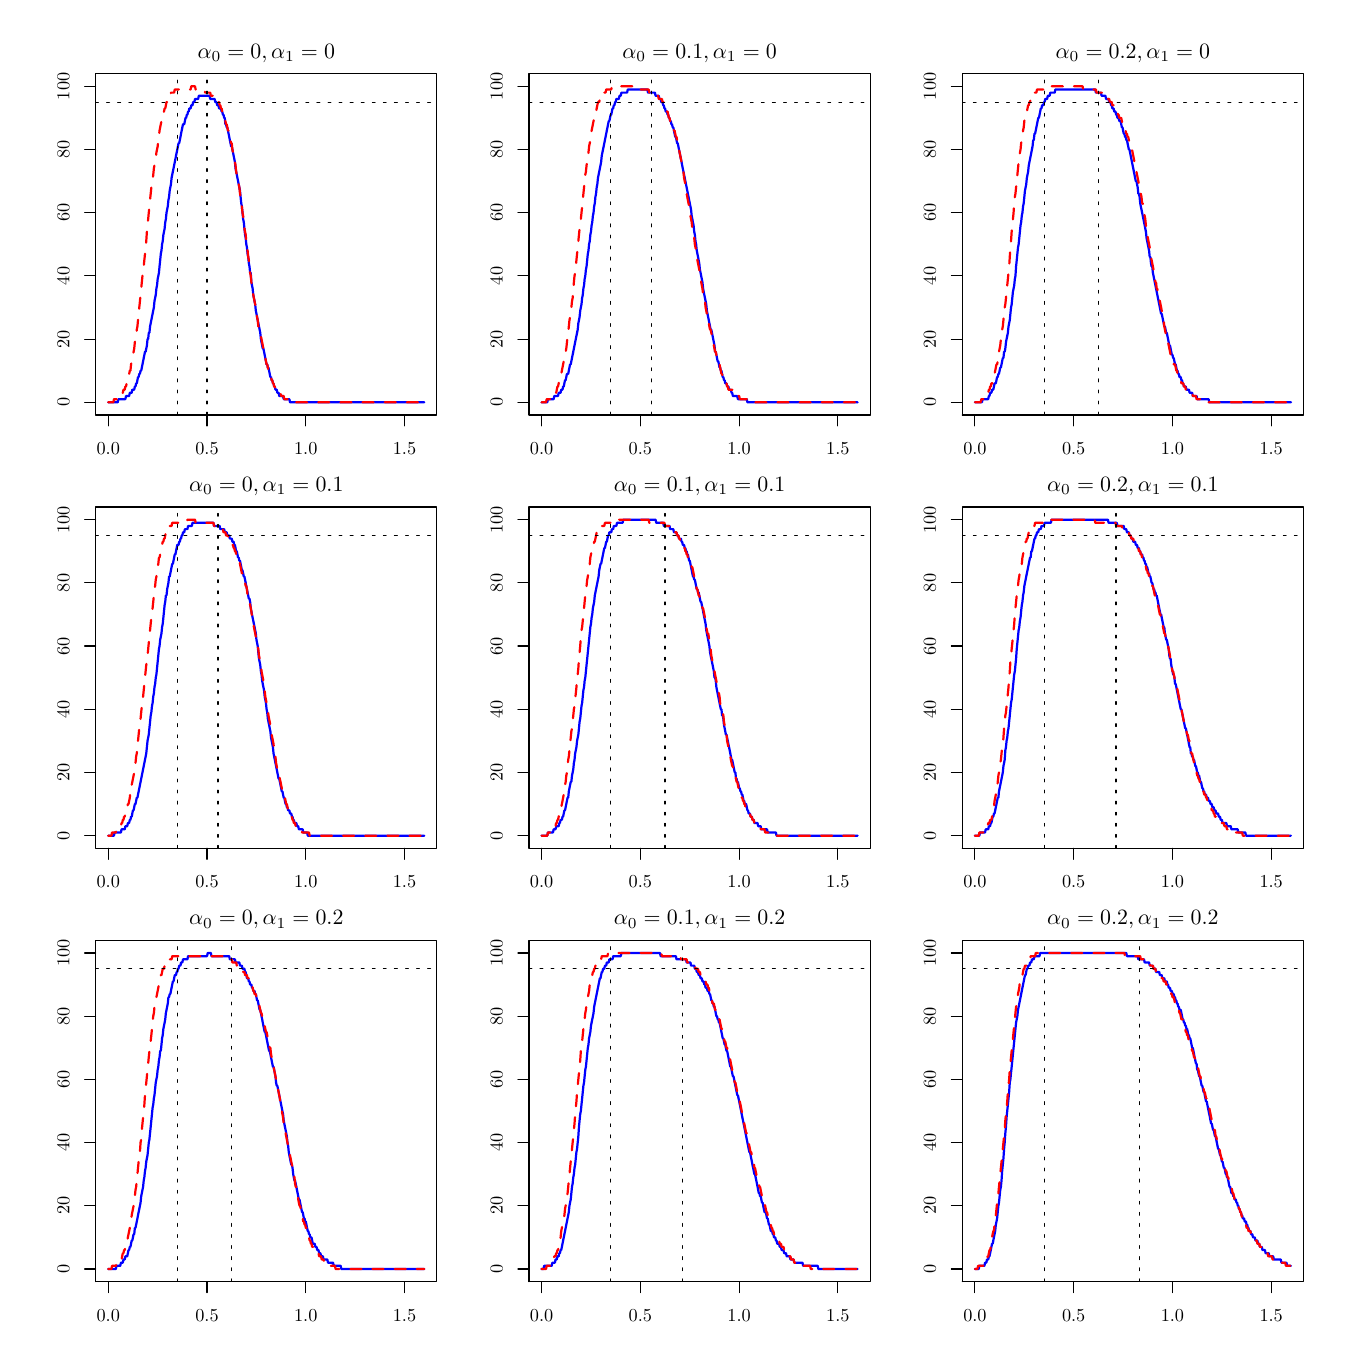
\begin{tikzpicture}[x=1pt,y=1pt]
\definecolor{fillColor}{RGB}{255,255,255}
\path[use as bounding box,fill=fillColor,fill opacity=0.00] (0,0) rectangle (469.75,469.75);
\begin{scope}
\path[clip] ( 24.55,329.80) rectangle (147.87,453.12);
\definecolor{drawColor}{RGB}{0,0,255}

\path[draw=drawColor,line width= 0.8pt,line join=round,line cap=round] ( 29.12,334.37) --
	( 29.35,334.37) --
	( 29.58,334.37) --
	( 29.81,334.37) --
	( 30.03,334.37) --
	( 30.26,334.37) --
	( 30.49,334.37) --
	( 30.72,334.37) --
	( 30.95,334.37) --
	( 31.18,334.37) --
	( 31.41,334.37) --
	( 31.64,334.37) --
	( 31.87,334.37) --
	( 32.09,334.37) --
	( 32.32,334.37) --
	( 32.55,334.37) --
	( 32.78,335.51) --
	( 33.01,335.51) --
	( 33.24,335.51) --
	( 33.47,335.51) --
	( 33.70,335.51) --
	( 33.92,335.51) --
	( 34.15,335.51) --
	( 34.38,335.51) --
	( 34.61,335.51) --
	( 34.84,335.51) --
	( 35.07,335.51) --
	( 35.30,335.51) --
	( 35.53,336.65) --
	( 35.76,336.65) --
	( 35.98,336.65) --
	( 36.21,336.65) --
	( 36.44,336.65) --
	( 36.67,336.65) --
	( 36.90,337.80) --
	( 37.13,337.80) --
	( 37.36,337.80) --
	( 37.59,337.80) --
	( 37.81,338.94) --
	( 38.04,338.94) --
	( 38.27,338.94) --
	( 38.50,338.94) --
	( 38.73,340.08) --
	( 38.96,340.08) --
	( 39.19,341.22) --
	( 39.42,341.22) --
	( 39.65,342.36) --
	( 39.87,343.50) --
	( 40.10,343.50) --
	( 40.33,344.65) --
	( 40.56,344.65) --
	( 40.79,345.79) --
	( 41.02,345.79) --
	( 41.25,346.93) --
	( 41.48,348.07) --
	( 41.71,349.21) --
	( 41.93,350.36) --
	( 42.16,351.50) --
	( 42.39,352.64) --
	( 42.62,352.64) --
	( 42.85,353.78) --
	( 43.08,354.92) --
	( 43.31,357.21) --
	( 43.54,357.21) --
	( 43.76,359.49) --
	( 43.99,359.49) --
	( 44.22,361.77) --
	( 44.45,362.92) --
	( 44.68,364.06) --
	( 44.91,365.20) --
	( 45.14,366.34) --
	( 45.37,367.48) --
	( 45.60,368.63) --
	( 45.82,370.91) --
	( 46.05,372.05) --
	( 46.28,373.19) --
	( 46.51,375.48) --
	( 46.74,376.62) --
	( 46.97,378.90) --
	( 47.20,380.04) --
	( 47.43,381.19) --
	( 47.65,383.47) --
	( 47.88,385.75) --
	( 48.11,388.04) --
	( 48.34,389.18) --
	( 48.57,391.46) --
	( 48.80,392.60) --
	( 49.03,394.89) --
	( 49.26,396.03) --
	( 49.49,397.17) --
	( 49.71,399.46) --
	( 49.94,400.60) --
	( 50.17,402.88) --
	( 50.40,404.02) --
	( 50.63,405.16) --
	( 50.86,407.45) --
	( 51.09,408.59) --
	( 51.32,410.87) --
	( 51.54,412.02) --
	( 51.77,413.16) --
	( 52.00,415.44) --
	( 52.23,416.58) --
	( 52.46,417.73) --
	( 52.69,418.87) --
	( 52.92,420.01) --
	( 53.15,421.15) --
	( 53.38,422.29) --
	( 53.60,423.43) --
	( 53.83,424.58) --
	( 54.06,425.72) --
	( 54.29,426.86) --
	( 54.52,428.00) --
	( 54.75,428.00) --
	( 54.98,429.14) --
	( 55.21,430.29) --
	( 55.43,431.43) --
	( 55.66,432.57) --
	( 55.89,433.71) --
	( 56.12,434.85) --
	( 56.35,434.85) --
	( 56.58,434.85) --
	( 56.81,436.00) --
	( 57.04,437.14) --
	( 57.27,437.14) --
	( 57.49,438.28) --
	( 57.72,438.28) --
	( 57.95,439.42) --
	( 58.18,439.42) --
	( 58.41,440.56) --
	( 58.64,440.56) --
	( 58.87,440.56) --
	( 59.10,441.70) --
	( 59.32,441.70) --
	( 59.55,441.70) --
	( 59.78,442.85) --
	( 60.01,442.85) --
	( 60.24,442.85) --
	( 60.47,443.99) --
	( 60.70,443.99) --
	( 60.93,443.99) --
	( 61.16,443.99) --
	( 61.38,443.99) --
	( 61.61,443.99) --
	( 61.84,445.13) --
	( 62.07,445.13) --
	( 62.30,445.13) --
	( 62.53,445.13) --
	( 62.76,445.13) --
	( 62.99,445.13) --
	( 63.22,445.13) --
	( 63.44,445.13) --
	( 63.67,445.13) --
	( 63.90,445.13) --
	( 64.13,445.13) --
	( 64.36,445.13) --
	( 64.59,445.13) --
	( 64.82,445.13) --
	( 65.05,445.13) --
	( 65.27,445.13) --
	( 65.50,445.13) --
	( 65.73,445.13) --
	( 65.96,443.99) --
	( 66.19,443.99) --
	( 66.42,443.99) --
	( 66.65,443.99) --
	( 66.88,443.99) --
	( 67.11,443.99) --
	( 67.33,443.99) --
	( 67.56,443.99) --
	( 67.79,442.85) --
	( 68.02,442.85) --
	( 68.25,442.85) --
	( 68.48,441.70) --
	( 68.71,441.70) --
	( 68.94,441.70) --
	( 69.16,440.56) --
	( 69.39,440.56) --
	( 69.62,440.56) --
	( 69.85,440.56) --
	( 70.08,439.42) --
	( 70.31,439.42) --
	( 70.54,438.28) --
	( 70.77,438.28) --
	( 71.00,437.14) --
	( 71.22,437.14) --
	( 71.45,434.85) --
	( 71.68,434.85) --
	( 71.91,433.71) --
	( 72.14,433.71) --
	( 72.37,432.57) --
	( 72.60,431.43) --
	( 72.83,430.29) --
	( 73.05,429.14) --
	( 73.28,428.00) --
	( 73.51,426.86) --
	( 73.74,426.86) --
	( 73.97,425.72) --
	( 74.20,424.58) --
	( 74.43,423.43) --
	( 74.66,422.29) --
	( 74.89,421.15) --
	( 75.11,418.87) --
	( 75.34,417.73) --
	( 75.57,416.58) --
	( 75.80,415.44) --
	( 76.03,414.30) --
	( 76.26,413.16) --
	( 76.49,412.02) --
	( 76.72,410.87) --
	( 76.94,408.59) --
	( 77.17,406.31) --
	( 77.40,405.16) --
	( 77.63,402.88) --
	( 77.86,400.60) --
	( 78.09,399.46) --
	( 78.32,397.17) --
	( 78.55,394.89) --
	( 78.78,393.75) --
	( 79.00,391.46) --
	( 79.23,390.32) --
	( 79.46,388.04) --
	( 79.69,386.90) --
	( 79.92,384.61) --
	( 80.15,383.47) --
	( 80.38,381.19) --
	( 80.61,381.19) --
	( 80.83,377.76) --
	( 81.06,376.62) --
	( 81.29,375.48) --
	( 81.52,373.19) --
	( 81.75,372.05) --
	( 81.98,370.91) --
	( 82.21,369.77) --
	( 82.44,367.48) --
	( 82.67,366.34) --
	( 82.89,365.20) --
	( 83.12,364.06) --
	( 83.35,362.92) --
	( 83.58,361.77) --
	( 83.81,360.63) --
	( 84.04,359.49) --
	( 84.27,357.21) --
	( 84.50,356.06) --
	( 84.73,354.92) --
	( 84.95,353.78) --
	( 85.18,353.78) --
	( 85.41,352.64) --
	( 85.64,351.50) --
	( 85.87,350.36) --
	( 86.10,349.21) --
	( 86.33,348.07) --
	( 86.56,348.07) --
	( 86.78,346.93) --
	( 87.01,346.93) --
	( 87.24,345.79) --
	( 87.47,344.65) --
	( 87.70,343.50) --
	( 87.93,343.50) --
	( 88.16,342.36) --
	( 88.39,342.36) --
	( 88.62,341.22) --
	( 88.84,341.22) --
	( 89.07,340.08) --
	( 89.30,340.08) --
	( 89.53,338.94) --
	( 89.76,338.94) --
	( 89.99,338.94) --
	( 90.22,337.80) --
	( 90.45,337.80) --
	( 90.67,337.80) --
	( 90.90,336.65) --
	( 91.13,336.65) --
	( 91.36,336.65) --
	( 91.59,336.65) --
	( 91.82,336.65) --
	( 92.05,336.65) --
	( 92.28,336.65) --
	( 92.51,335.51) --
	( 92.73,335.51) --
	( 92.96,335.51) --
	( 93.19,335.51) --
	( 93.42,335.51) --
	( 93.65,335.51) --
	( 93.88,335.51) --
	( 94.11,335.51) --
	( 94.34,335.51) --
	( 94.56,335.51) --
	( 94.79,334.37) --
	( 95.02,334.37) --
	( 95.25,334.37) --
	( 95.48,334.37) --
	( 95.71,334.37) --
	( 95.94,334.37) --
	( 96.17,334.37) --
	( 96.40,334.37) --
	( 96.62,334.37) --
	( 96.85,334.37) --
	( 97.08,334.37) --
	( 97.31,334.37) --
	( 97.54,334.37) --
	( 97.77,334.37) --
	( 98.00,334.37) --
	( 98.23,334.37) --
	( 98.45,334.37) --
	( 98.68,334.37) --
	( 98.91,334.37) --
	( 99.14,334.37) --
	( 99.37,334.37) --
	( 99.60,334.37) --
	( 99.83,334.37) --
	(100.06,334.37) --
	(100.29,334.37) --
	(100.51,334.37) --
	(100.74,334.37) --
	(100.97,334.37) --
	(101.20,334.37) --
	(101.43,334.37) --
	(101.66,334.37) --
	(101.89,334.37) --
	(102.12,334.37) --
	(102.35,334.37) --
	(102.57,334.37) --
	(102.80,334.37) --
	(103.03,334.37) --
	(103.26,334.37) --
	(103.49,334.37) --
	(103.72,334.37) --
	(103.95,334.37) --
	(104.18,334.37) --
	(104.40,334.37) --
	(104.63,334.37) --
	(104.86,334.37) --
	(105.09,334.37) --
	(105.32,334.37) --
	(105.55,334.37) --
	(105.78,334.37) --
	(106.01,334.37) --
	(106.24,334.37) --
	(106.46,334.37) --
	(106.69,334.37) --
	(106.92,334.37) --
	(107.15,334.37) --
	(107.38,334.37) --
	(107.61,334.37) --
	(107.84,334.37) --
	(108.07,334.37) --
	(108.29,334.37) --
	(108.52,334.37) --
	(108.75,334.37) --
	(108.98,334.37) --
	(109.21,334.37) --
	(109.44,334.37) --
	(109.67,334.37) --
	(109.90,334.37) --
	(110.13,334.37) --
	(110.35,334.37) --
	(110.58,334.37) --
	(110.81,334.37) --
	(111.04,334.37) --
	(111.27,334.37) --
	(111.50,334.37) --
	(111.73,334.37) --
	(111.96,334.37) --
	(112.18,334.37) --
	(112.41,334.37) --
	(112.64,334.37) --
	(112.87,334.37) --
	(113.10,334.37) --
	(113.33,334.37) --
	(113.56,334.37) --
	(113.79,334.37) --
	(114.02,334.37) --
	(114.24,334.37) --
	(114.47,334.37) --
	(114.70,334.37) --
	(114.93,334.37) --
	(115.16,334.37) --
	(115.39,334.37) --
	(115.62,334.37) --
	(115.85,334.37) --
	(116.07,334.37) --
	(116.30,334.37) --
	(116.53,334.37) --
	(116.76,334.37) --
	(116.99,334.37) --
	(117.22,334.37) --
	(117.45,334.37) --
	(117.68,334.37) --
	(117.91,334.37) --
	(118.13,334.37) --
	(118.36,334.37) --
	(118.59,334.37) --
	(118.82,334.37) --
	(119.05,334.37) --
	(119.28,334.37) --
	(119.51,334.37) --
	(119.74,334.37) --
	(119.96,334.37) --
	(120.19,334.37) --
	(120.42,334.37) --
	(120.65,334.37) --
	(120.88,334.37) --
	(121.11,334.37) --
	(121.34,334.37) --
	(121.57,334.37) --
	(121.80,334.37) --
	(122.02,334.37) --
	(122.25,334.37) --
	(122.48,334.37) --
	(122.71,334.37) --
	(122.94,334.37) --
	(123.17,334.37) --
	(123.40,334.37) --
	(123.63,334.37) --
	(123.86,334.37) --
	(124.08,334.37) --
	(124.31,334.37) --
	(124.54,334.37) --
	(124.77,334.37) --
	(125.00,334.37) --
	(125.23,334.37) --
	(125.46,334.37) --
	(125.69,334.37) --
	(125.91,334.37) --
	(126.14,334.37) --
	(126.37,334.37) --
	(126.60,334.37) --
	(126.83,334.37) --
	(127.06,334.37) --
	(127.29,334.37) --
	(127.52,334.37) --
	(127.75,334.37) --
	(127.97,334.37) --
	(128.20,334.37) --
	(128.43,334.37) --
	(128.66,334.37) --
	(128.89,334.37) --
	(129.12,334.37) --
	(129.35,334.37) --
	(129.58,334.37) --
	(129.80,334.37) --
	(130.03,334.37) --
	(130.26,334.37) --
	(130.49,334.37) --
	(130.72,334.37) --
	(130.95,334.37) --
	(131.18,334.37) --
	(131.41,334.37) --
	(131.64,334.37) --
	(131.86,334.37) --
	(132.09,334.37) --
	(132.32,334.37) --
	(132.55,334.37) --
	(132.78,334.37) --
	(133.01,334.37) --
	(133.24,334.37) --
	(133.47,334.37) --
	(133.69,334.37) --
	(133.92,334.37) --
	(134.15,334.37) --
	(134.38,334.37) --
	(134.61,334.37) --
	(134.84,334.37) --
	(135.07,334.37) --
	(135.30,334.37) --
	(135.53,334.37) --
	(135.75,334.37) --
	(135.98,334.37) --
	(136.21,334.37) --
	(136.44,334.37) --
	(136.67,334.37) --
	(136.90,334.37) --
	(137.13,334.37) --
	(137.36,334.37) --
	(137.58,334.37) --
	(137.81,334.37) --
	(138.04,334.37) --
	(138.27,334.37) --
	(138.50,334.37) --
	(138.73,334.37) --
	(138.96,334.37) --
	(139.19,334.37) --
	(139.42,334.37) --
	(139.64,334.37) --
	(139.87,334.37) --
	(140.10,334.37) --
	(140.33,334.37) --
	(140.56,334.37) --
	(140.79,334.37) --
	(141.02,334.37) --
	(141.25,334.37) --
	(141.47,334.37) --
	(141.70,334.37) --
	(141.93,334.37) --
	(142.16,334.37) --
	(142.39,334.37) --
	(142.62,334.37) --
	(142.85,334.37) --
	(143.08,334.37) --
	(143.31,334.37);
\end{scope}
\begin{scope}
\path[clip] (  0.00,  0.00) rectangle (469.75,469.75);
\definecolor{drawColor}{RGB}{0,0,0}

\path[draw=drawColor,line width= 0.4pt,line join=round,line cap=round] ( 29.12,329.80) -- (136.17,329.80);

\path[draw=drawColor,line width= 0.4pt,line join=round,line cap=round] ( 29.12,329.80) -- ( 29.12,325.84);

\path[draw=drawColor,line width= 0.4pt,line join=round,line cap=round] ( 64.80,329.80) -- ( 64.80,325.84);

\path[draw=drawColor,line width= 0.4pt,line join=round,line cap=round] (100.49,329.80) -- (100.49,325.84);

\path[draw=drawColor,line width= 0.4pt,line join=round,line cap=round] (136.17,329.80) -- (136.17,325.84);

\node[text=drawColor,anchor=base,inner sep=0pt, outer sep=0pt, scale=  0.66] at ( 29.12,315.55) {0.0};

\node[text=drawColor,anchor=base,inner sep=0pt, outer sep=0pt, scale=  0.66] at ( 64.80,315.55) {0.5};

\node[text=drawColor,anchor=base,inner sep=0pt, outer sep=0pt, scale=  0.66] at (100.49,315.55) {1.0};

\node[text=drawColor,anchor=base,inner sep=0pt, outer sep=0pt, scale=  0.66] at (136.17,315.55) {1.5};

\path[draw=drawColor,line width= 0.4pt,line join=round,line cap=round] ( 24.55,334.37) -- ( 24.55,448.56);

\path[draw=drawColor,line width= 0.4pt,line join=round,line cap=round] ( 24.55,334.37) -- ( 20.59,334.37);

\path[draw=drawColor,line width= 0.4pt,line join=round,line cap=round] ( 24.55,357.21) -- ( 20.59,357.21);

\path[draw=drawColor,line width= 0.4pt,line join=round,line cap=round] ( 24.55,380.04) -- ( 20.59,380.04);

\path[draw=drawColor,line width= 0.4pt,line join=round,line cap=round] ( 24.55,402.88) -- ( 20.59,402.88);

\path[draw=drawColor,line width= 0.4pt,line join=round,line cap=round] ( 24.55,425.72) -- ( 20.59,425.72);

\path[draw=drawColor,line width= 0.4pt,line join=round,line cap=round] ( 24.55,448.56) -- ( 20.59,448.56);

\node[text=drawColor,rotate= 90.00,anchor=base,inner sep=0pt, outer sep=0pt, scale=  0.66] at ( 15.05,334.37) {0};

\node[text=drawColor,rotate= 90.00,anchor=base,inner sep=0pt, outer sep=0pt, scale=  0.66] at ( 15.05,357.21) {20};

\node[text=drawColor,rotate= 90.00,anchor=base,inner sep=0pt, outer sep=0pt, scale=  0.66] at ( 15.05,380.04) {40};

\node[text=drawColor,rotate= 90.00,anchor=base,inner sep=0pt, outer sep=0pt, scale=  0.66] at ( 15.05,402.88) {60};

\node[text=drawColor,rotate= 90.00,anchor=base,inner sep=0pt, outer sep=0pt, scale=  0.66] at ( 15.05,425.72) {80};

\node[text=drawColor,rotate= 90.00,anchor=base,inner sep=0pt, outer sep=0pt, scale=  0.66] at ( 15.05,448.56) {100};

\path[draw=drawColor,line width= 0.4pt,line join=round,line cap=round] ( 24.55,329.80) --
	(147.87,329.80) --
	(147.87,453.12) --
	( 24.55,453.12) --
	( 24.55,329.80);
\end{scope}
\begin{scope}
\path[clip] (  0.00,313.17) rectangle (156.58,469.75);
\definecolor{drawColor}{RGB}{0,0,0}

\node[text=drawColor,anchor=base,inner sep=0pt, outer sep=0pt, scale=  0.79] at ( 86.21,458.71) {\bfseries $\alpha_0 = 0, \alpha_1 = 0$};
\end{scope}
\begin{scope}
\path[clip] ( 24.55,329.80) rectangle (147.87,453.12);
\definecolor{drawColor}{RGB}{255,0,0}

\path[draw=drawColor,line width= 0.8pt,dash pattern=on 4pt off 4pt ,line join=round,line cap=round] ( 29.12,334.37) --
	( 29.35,334.37) --
	( 29.58,334.37) --
	( 29.81,334.37) --
	( 30.03,334.37) --
	( 30.26,334.37) --
	( 30.49,334.37) --
	( 30.72,334.37) --
	( 30.95,334.37) --
	( 31.18,335.51) --
	( 31.41,335.51) --
	( 31.64,335.51) --
	( 31.87,335.51) --
	( 32.09,335.51) --
	( 32.32,335.51) --
	( 32.55,335.51) --
	( 32.78,335.51) --
	( 33.01,336.65) --
	( 33.24,336.65) --
	( 33.47,336.65) --
	( 33.70,336.65) --
	( 33.92,337.80) --
	( 34.15,337.80) --
	( 34.38,337.80) --
	( 34.61,338.94) --
	( 34.84,338.94) --
	( 35.07,338.94) --
	( 35.30,340.08) --
	( 35.53,340.08) --
	( 35.76,341.22) --
	( 35.98,341.22) --
	( 36.21,342.36) --
	( 36.44,343.50) --
	( 36.67,344.65) --
	( 36.90,345.79) --
	( 37.13,345.79) --
	( 37.36,348.07) --
	( 37.59,349.21) --
	( 37.81,350.36) --
	( 38.04,351.50) --
	( 38.27,352.64) --
	( 38.50,353.78) --
	( 38.73,356.06) --
	( 38.96,357.21) --
	( 39.19,358.35) --
	( 39.42,360.63) --
	( 39.65,361.77) --
	( 39.87,364.06) --
	( 40.10,366.34) --
	( 40.33,368.63) --
	( 40.56,370.91) --
	( 40.79,373.19) --
	( 41.02,375.48) --
	( 41.25,377.76) --
	( 41.48,380.04) --
	( 41.71,381.19) --
	( 41.93,383.47) --
	( 42.16,385.75) --
	( 42.39,388.04) --
	( 42.62,390.32) --
	( 42.85,392.60) --
	( 43.08,396.03) --
	( 43.31,398.31) --
	( 43.54,400.60) --
	( 43.76,402.88) --
	( 43.99,405.16) --
	( 44.22,407.45) --
	( 44.45,409.73) --
	( 44.68,412.02) --
	( 44.91,413.16) --
	( 45.14,414.30) --
	( 45.37,416.58) --
	( 45.60,418.87) --
	( 45.82,420.01) --
	( 46.05,421.15) --
	( 46.28,422.29) --
	( 46.51,424.58) --
	( 46.74,425.72) --
	( 46.97,426.86) --
	( 47.20,429.14) --
	( 47.43,430.29) --
	( 47.65,432.57) --
	( 47.88,433.71) --
	( 48.11,434.85) --
	( 48.34,436.00) --
	( 48.57,437.14) --
	( 48.80,438.28) --
	( 49.03,438.28) --
	( 49.26,439.42) --
	( 49.49,440.56) --
	( 49.71,440.56) --
	( 49.94,441.70) --
	( 50.17,442.85) --
	( 50.40,442.85) --
	( 50.63,443.99) --
	( 50.86,443.99) --
	( 51.09,445.13) --
	( 51.32,445.13) --
	( 51.54,445.13) --
	( 51.77,446.27) --
	( 52.00,446.27) --
	( 52.23,446.27) --
	( 52.46,446.27) --
	( 52.69,446.27) --
	( 52.92,446.27) --
	( 53.15,447.41) --
	( 53.38,447.41) --
	( 53.60,447.41) --
	( 53.83,447.41) --
	( 54.06,447.41) --
	( 54.29,447.41) --
	( 54.52,447.41) --
	( 54.75,447.41) --
	( 54.98,447.41) --
	( 55.21,447.41) --
	( 55.43,447.41) --
	( 55.66,447.41) --
	( 55.89,447.41) --
	( 56.12,447.41) --
	( 56.35,447.41) --
	( 56.58,447.41) --
	( 56.81,447.41) --
	( 57.04,447.41) --
	( 57.27,447.41) --
	( 57.49,447.41) --
	( 57.72,447.41) --
	( 57.95,447.41) --
	( 58.18,447.41) --
	( 58.41,447.41) --
	( 58.64,447.41) --
	( 58.87,447.41) --
	( 59.10,448.56) --
	( 59.32,448.56) --
	( 59.55,448.56) --
	( 59.78,448.56) --
	( 60.01,448.56) --
	( 60.24,448.56) --
	( 60.47,448.56) --
	( 60.70,447.41) --
	( 60.93,447.41) --
	( 61.16,447.41) --
	( 61.38,447.41) --
	( 61.61,447.41) --
	( 61.84,447.41) --
	( 62.07,447.41) --
	( 62.30,447.41) --
	( 62.53,447.41) --
	( 62.76,447.41) --
	( 62.99,447.41) --
	( 63.22,447.41) --
	( 63.44,447.41) --
	( 63.67,447.41) --
	( 63.90,447.41) --
	( 64.13,446.27) --
	( 64.36,446.27) --
	( 64.59,446.27) --
	( 64.82,446.27) --
	( 65.05,446.27) --
	( 65.27,446.27) --
	( 65.50,446.27) --
	( 65.73,446.27) --
	( 65.96,446.27) --
	( 66.19,445.13) --
	( 66.42,445.13) --
	( 66.65,445.13) --
	( 66.88,445.13) --
	( 67.11,445.13) --
	( 67.33,443.99) --
	( 67.56,443.99) --
	( 67.79,443.99) --
	( 68.02,443.99) --
	( 68.25,443.99) --
	( 68.48,442.85) --
	( 68.71,442.85) --
	( 68.94,442.85) --
	( 69.16,442.85) --
	( 69.39,441.70) --
	( 69.62,441.70) --
	( 69.85,440.56) --
	( 70.08,440.56) --
	( 70.31,439.42) --
	( 70.54,438.28) --
	( 70.77,438.28) --
	( 71.00,437.14) --
	( 71.22,437.14) --
	( 71.45,436.00) --
	( 71.68,434.85) --
	( 71.91,434.85) --
	( 72.14,433.71) --
	( 72.37,432.57) --
	( 72.60,432.57) --
	( 72.83,431.43) --
	( 73.05,430.29) --
	( 73.28,429.14) --
	( 73.51,428.00) --
	( 73.74,428.00) --
	( 73.97,425.72) --
	( 74.20,424.58) --
	( 74.43,423.43) --
	( 74.66,422.29) --
	( 74.89,421.15) --
	( 75.11,420.01) --
	( 75.34,417.73) --
	( 75.57,416.58) --
	( 75.80,415.44) --
	( 76.03,414.30) --
	( 76.26,413.16) --
	( 76.49,412.02) --
	( 76.72,409.73) --
	( 76.94,408.59) --
	( 77.17,407.45) --
	( 77.40,405.16) --
	( 77.63,402.88) --
	( 77.86,401.74) --
	( 78.09,399.46) --
	( 78.32,397.17) --
	( 78.55,396.03) --
	( 78.78,394.89) --
	( 79.00,392.60) --
	( 79.23,390.32) --
	( 79.46,389.18) --
	( 79.69,386.90) --
	( 79.92,385.75) --
	( 80.15,383.47) --
	( 80.38,381.19) --
	( 80.61,380.04) --
	( 80.83,377.76) --
	( 81.06,376.62) --
	( 81.29,374.33) --
	( 81.52,373.19) --
	( 81.75,372.05) --
	( 81.98,370.91) --
	( 82.21,369.77) --
	( 82.44,368.63) --
	( 82.67,366.34) --
	( 82.89,365.20) --
	( 83.12,364.06) --
	( 83.35,361.77) --
	( 83.58,361.77) --
	( 83.81,360.63) --
	( 84.04,359.49) --
	( 84.27,358.35) --
	( 84.50,357.21) --
	( 84.73,356.06) --
	( 84.95,354.92) --
	( 85.18,353.78) --
	( 85.41,352.64) --
	( 85.64,351.50) --
	( 85.87,350.36) --
	( 86.10,349.21) --
	( 86.33,348.07) --
	( 86.56,348.07) --
	( 86.78,346.93) --
	( 87.01,345.79) --
	( 87.24,344.65) --
	( 87.47,344.65) --
	( 87.70,343.50) --
	( 87.93,343.50) --
	( 88.16,342.36) --
	( 88.39,342.36) --
	( 88.62,341.22) --
	( 88.84,341.22) --
	( 89.07,340.08) --
	( 89.30,340.08) --
	( 89.53,338.94) --
	( 89.76,338.94) --
	( 89.99,338.94) --
	( 90.22,338.94) --
	( 90.45,337.80) --
	( 90.67,337.80) --
	( 90.90,337.80) --
	( 91.13,337.80) --
	( 91.36,337.80) --
	( 91.59,336.65) --
	( 91.82,336.65) --
	( 92.05,336.65) --
	( 92.28,336.65) --
	( 92.51,336.65) --
	( 92.73,335.51) --
	( 92.96,335.51) --
	( 93.19,335.51) --
	( 93.42,335.51) --
	( 93.65,335.51) --
	( 93.88,335.51) --
	( 94.11,335.51) --
	( 94.34,335.51) --
	( 94.56,335.51) --
	( 94.79,334.37) --
	( 95.02,334.37) --
	( 95.25,334.37) --
	( 95.48,334.37) --
	( 95.71,334.37) --
	( 95.94,334.37) --
	( 96.17,334.37) --
	( 96.40,334.37) --
	( 96.62,334.37) --
	( 96.85,334.37) --
	( 97.08,334.37) --
	( 97.31,334.37) --
	( 97.54,334.37) --
	( 97.77,334.37) --
	( 98.00,334.37) --
	( 98.23,334.37) --
	( 98.45,334.37) --
	( 98.68,334.37) --
	( 98.91,334.37) --
	( 99.14,334.37) --
	( 99.37,334.37) --
	( 99.60,334.37) --
	( 99.83,334.37) --
	(100.06,334.37) --
	(100.29,334.37) --
	(100.51,334.37) --
	(100.74,334.37) --
	(100.97,334.37) --
	(101.20,334.37) --
	(101.43,334.37) --
	(101.66,334.37) --
	(101.89,334.37) --
	(102.12,334.37) --
	(102.35,334.37) --
	(102.57,334.37) --
	(102.80,334.37) --
	(103.03,334.37) --
	(103.26,334.37) --
	(103.49,334.37) --
	(103.72,334.37) --
	(103.95,334.37) --
	(104.18,334.37) --
	(104.40,334.37) --
	(104.63,334.37) --
	(104.86,334.37) --
	(105.09,334.37) --
	(105.32,334.37) --
	(105.55,334.37) --
	(105.78,334.37) --
	(106.01,334.37) --
	(106.24,334.37) --
	(106.46,334.37) --
	(106.69,334.37) --
	(106.92,334.37) --
	(107.15,334.37) --
	(107.38,334.37) --
	(107.61,334.37) --
	(107.84,334.37) --
	(108.07,334.37) --
	(108.29,334.37) --
	(108.52,334.37) --
	(108.75,334.37) --
	(108.98,334.37) --
	(109.21,334.37) --
	(109.44,334.37) --
	(109.67,334.37) --
	(109.90,334.37) --
	(110.13,334.37) --
	(110.35,334.37) --
	(110.58,334.37) --
	(110.81,334.37) --
	(111.04,334.37) --
	(111.27,334.37) --
	(111.50,334.37) --
	(111.73,334.37) --
	(111.96,334.37) --
	(112.18,334.37) --
	(112.41,334.37) --
	(112.64,334.37) --
	(112.87,334.37) --
	(113.10,334.37) --
	(113.33,334.37) --
	(113.56,334.37) --
	(113.79,334.37) --
	(114.02,334.37) --
	(114.24,334.37) --
	(114.47,334.37) --
	(114.70,334.37) --
	(114.93,334.37) --
	(115.16,334.37) --
	(115.39,334.37) --
	(115.62,334.37) --
	(115.85,334.37) --
	(116.07,334.37) --
	(116.30,334.37) --
	(116.53,334.37) --
	(116.76,334.37) --
	(116.99,334.37) --
	(117.22,334.37) --
	(117.45,334.37) --
	(117.68,334.37) --
	(117.91,334.37) --
	(118.13,334.37) --
	(118.36,334.37) --
	(118.59,334.37) --
	(118.82,334.37) --
	(119.05,334.37) --
	(119.28,334.37) --
	(119.51,334.37) --
	(119.74,334.37) --
	(119.96,334.37) --
	(120.19,334.37) --
	(120.42,334.37) --
	(120.65,334.37) --
	(120.88,334.37) --
	(121.11,334.37) --
	(121.34,334.37) --
	(121.57,334.37) --
	(121.80,334.37) --
	(122.02,334.37) --
	(122.25,334.37) --
	(122.48,334.37) --
	(122.71,334.37) --
	(122.94,334.37) --
	(123.17,334.37) --
	(123.40,334.37) --
	(123.63,334.37) --
	(123.86,334.37) --
	(124.08,334.37) --
	(124.31,334.37) --
	(124.54,334.37) --
	(124.77,334.37) --
	(125.00,334.37) --
	(125.23,334.37) --
	(125.46,334.37) --
	(125.69,334.37) --
	(125.91,334.37) --
	(126.14,334.37) --
	(126.37,334.37) --
	(126.60,334.37) --
	(126.83,334.37) --
	(127.06,334.37) --
	(127.29,334.37) --
	(127.52,334.37) --
	(127.75,334.37) --
	(127.97,334.37) --
	(128.20,334.37) --
	(128.43,334.37) --
	(128.66,334.37) --
	(128.89,334.37) --
	(129.12,334.37) --
	(129.35,334.37) --
	(129.58,334.37) --
	(129.80,334.37) --
	(130.03,334.37) --
	(130.26,334.37) --
	(130.49,334.37) --
	(130.72,334.37) --
	(130.95,334.37) --
	(131.18,334.37) --
	(131.41,334.37) --
	(131.64,334.37) --
	(131.86,334.37) --
	(132.09,334.37) --
	(132.32,334.37) --
	(132.55,334.37) --
	(132.78,334.37) --
	(133.01,334.37) --
	(133.24,334.37) --
	(133.47,334.37) --
	(133.69,334.37) --
	(133.92,334.37) --
	(134.15,334.37) --
	(134.38,334.37) --
	(134.61,334.37) --
	(134.84,334.37) --
	(135.07,334.37) --
	(135.30,334.37) --
	(135.53,334.37) --
	(135.75,334.37) --
	(135.98,334.37) --
	(136.21,334.37) --
	(136.44,334.37) --
	(136.67,334.37) --
	(136.90,334.37) --
	(137.13,334.37) --
	(137.36,334.37) --
	(137.58,334.37) --
	(137.81,334.37) --
	(138.04,334.37) --
	(138.27,334.37) --
	(138.50,334.37) --
	(138.73,334.37) --
	(138.96,334.37) --
	(139.19,334.37) --
	(139.42,334.37) --
	(139.64,334.37) --
	(139.87,334.37) --
	(140.10,334.37) --
	(140.33,334.37) --
	(140.56,334.37) --
	(140.79,334.37) --
	(141.02,334.37) --
	(141.25,334.37) --
	(141.47,334.37) --
	(141.70,334.37) --
	(141.93,334.37) --
	(142.16,334.37) --
	(142.39,334.37) --
	(142.62,334.37) --
	(142.85,334.37) --
	(143.08,334.37) --
	(143.31,334.37);
\definecolor{drawColor}{RGB}{0,0,0}

\path[draw=drawColor,line width= 0.4pt,dash pattern=on 1pt off 3pt ,line join=round,line cap=round] ( 24.55,442.85) -- (147.87,442.85);

\path[draw=drawColor,line width= 0.4pt,dash pattern=on 1pt off 3pt ,line join=round,line cap=round] ( 54.10,329.80) -- ( 54.10,453.12);

\path[draw=drawColor,line width= 0.4pt,dash pattern=on 1pt off 3pt ,line join=round,line cap=round] ( 64.80,329.80) -- ( 64.80,453.12);
\end{scope}
\begin{scope}
\path[clip] (181.14,329.80) rectangle (304.46,453.12);
\definecolor{drawColor}{RGB}{0,0,255}

\path[draw=drawColor,line width= 0.8pt,line join=round,line cap=round] (185.70,334.37) --
	(185.93,334.37) --
	(186.16,334.37) --
	(186.39,334.37) --
	(186.62,334.37) --
	(186.85,334.37) --
	(187.08,334.37) --
	(187.31,334.37) --
	(187.54,334.37) --
	(187.76,334.37) --
	(187.99,335.51) --
	(188.22,335.51) --
	(188.45,335.51) --
	(188.68,335.51) --
	(188.91,335.51) --
	(189.14,335.51) --
	(189.37,335.51) --
	(189.59,335.51) --
	(189.82,335.51) --
	(190.05,335.51) --
	(190.28,336.65) --
	(190.51,336.65) --
	(190.74,336.65) --
	(190.97,336.65) --
	(191.20,336.65) --
	(191.43,336.65) --
	(191.65,336.65) --
	(191.88,337.80) --
	(192.11,337.80) --
	(192.34,337.80) --
	(192.57,337.80) --
	(192.80,338.94) --
	(193.03,338.94) --
	(193.26,338.94) --
	(193.48,340.08) --
	(193.71,340.08) --
	(193.94,341.22) --
	(194.17,342.36) --
	(194.40,342.36) --
	(194.63,343.50) --
	(194.86,344.65) --
	(195.09,344.65) --
	(195.32,344.65) --
	(195.54,345.79) --
	(195.77,346.93) --
	(196.00,348.07) --
	(196.23,348.07) --
	(196.46,349.21) --
	(196.69,350.36) --
	(196.92,351.50) --
	(197.15,352.64) --
	(197.37,353.78) --
	(197.60,354.92) --
	(197.83,356.06) --
	(198.06,357.21) --
	(198.29,358.35) --
	(198.52,359.49) --
	(198.75,360.63) --
	(198.98,362.92) --
	(199.21,364.06) --
	(199.43,365.20) --
	(199.66,367.48) --
	(199.89,368.63) --
	(200.12,369.77) --
	(200.35,372.05) --
	(200.58,373.19) --
	(200.81,375.48) --
	(201.04,376.62) --
	(201.26,378.90) --
	(201.49,380.04) --
	(201.72,382.33) --
	(201.95,383.47) --
	(202.18,385.75) --
	(202.41,388.04) --
	(202.64,389.18) --
	(202.87,391.46) --
	(203.10,392.60) --
	(203.32,394.89) --
	(203.55,396.03) --
	(203.78,398.31) --
	(204.01,399.46) --
	(204.24,401.74) --
	(204.47,402.88) --
	(204.70,405.16) --
	(204.93,406.31) --
	(205.15,408.59) --
	(205.38,409.73) --
	(205.61,412.02) --
	(205.84,413.16) --
	(206.07,415.44) --
	(206.30,416.58) --
	(206.53,417.73) --
	(206.76,418.87) --
	(206.99,420.01) --
	(207.21,421.15) --
	(207.44,423.43) --
	(207.67,424.58) --
	(207.90,425.72) --
	(208.13,426.86) --
	(208.36,428.00) --
	(208.59,429.14) --
	(208.82,430.29) --
	(209.05,431.43) --
	(209.27,432.57) --
	(209.50,433.71) --
	(209.73,434.85) --
	(209.96,436.00) --
	(210.19,436.00) --
	(210.42,437.14) --
	(210.65,438.28) --
	(210.88,438.28) --
	(211.10,439.42) --
	(211.33,440.56) --
	(211.56,440.56) --
	(211.79,441.70) --
	(212.02,441.70) --
	(212.25,442.85) --
	(212.48,442.85) --
	(212.71,443.99) --
	(212.94,443.99) --
	(213.16,443.99) --
	(213.39,443.99) --
	(213.62,443.99) --
	(213.85,445.13) --
	(214.08,445.13) --
	(214.31,445.13) --
	(214.54,446.27) --
	(214.77,446.27) --
	(214.99,446.27) --
	(215.22,446.27) --
	(215.45,446.27) --
	(215.68,446.27) --
	(215.91,446.27) --
	(216.14,446.27) --
	(216.37,446.27) --
	(216.60,446.27) --
	(216.83,447.41) --
	(217.05,447.41) --
	(217.28,447.41) --
	(217.51,447.41) --
	(217.74,447.41) --
	(217.97,447.41) --
	(218.20,447.41) --
	(218.43,447.41) --
	(218.66,447.41) --
	(218.88,447.41) --
	(219.11,447.41) --
	(219.34,447.41) --
	(219.57,447.41) --
	(219.80,447.41) --
	(220.03,447.41) --
	(220.26,447.41) --
	(220.49,447.41) --
	(220.72,447.41) --
	(220.94,447.41) --
	(221.17,447.41) --
	(221.40,447.41) --
	(221.63,447.41) --
	(221.86,447.41) --
	(222.09,447.41) --
	(222.32,447.41) --
	(222.55,447.41) --
	(222.77,447.41) --
	(223.00,447.41) --
	(223.23,447.41) --
	(223.46,447.41) --
	(223.69,447.41) --
	(223.92,447.41) --
	(224.15,446.27) --
	(224.38,446.27) --
	(224.61,446.27) --
	(224.83,446.27) --
	(225.06,446.27) --
	(225.29,446.27) --
	(225.52,446.27) --
	(225.75,446.27) --
	(225.98,446.27) --
	(226.21,446.27) --
	(226.44,446.27) --
	(226.66,446.27) --
	(226.89,445.13) --
	(227.12,445.13) --
	(227.35,445.13) --
	(227.58,445.13) --
	(227.81,445.13) --
	(228.04,445.13) --
	(228.27,443.99) --
	(228.50,443.99) --
	(228.72,443.99) --
	(228.95,442.85) --
	(229.18,442.85) --
	(229.41,442.85) --
	(229.64,441.70) --
	(229.87,441.70) --
	(230.10,440.56) --
	(230.33,440.56) --
	(230.56,439.42) --
	(230.78,439.42) --
	(231.01,439.42) --
	(231.24,438.28) --
	(231.47,438.28) --
	(231.70,437.14) --
	(231.93,437.14) --
	(232.16,436.00) --
	(232.39,436.00) --
	(232.61,434.85) --
	(232.84,434.85) --
	(233.07,433.71) --
	(233.30,433.71) --
	(233.53,432.57) --
	(233.76,431.43) --
	(233.99,430.29) --
	(234.22,430.29) --
	(234.45,429.14) --
	(234.67,428.00) --
	(234.90,428.00) --
	(235.13,426.86) --
	(235.36,425.72) --
	(235.59,424.58) --
	(235.82,423.43) --
	(236.05,422.29) --
	(236.28,421.15) --
	(236.50,420.01) --
	(236.73,418.87) --
	(236.96,417.73) --
	(237.19,416.58) --
	(237.42,415.44) --
	(237.65,414.30) --
	(237.88,413.16) --
	(238.11,412.02) --
	(238.34,410.87) --
	(238.56,409.73) --
	(238.79,408.59) --
	(239.02,407.45) --
	(239.25,406.31) --
	(239.48,405.16) --
	(239.71,404.02) --
	(239.94,401.74) --
	(240.17,400.60) --
	(240.39,399.46) --
	(240.62,398.31) --
	(240.85,396.03) --
	(241.08,394.89) --
	(241.31,392.60) --
	(241.54,391.46) --
	(241.77,389.18) --
	(242.00,388.04) --
	(242.23,386.90) --
	(242.45,385.75) --
	(242.68,384.61) --
	(242.91,382.33) --
	(243.14,381.19) --
	(243.37,380.04) --
	(243.60,378.90) --
	(243.83,377.76) --
	(244.06,375.48) --
	(244.28,374.33) --
	(244.51,373.19) --
	(244.74,372.05) --
	(244.97,370.91) --
	(245.20,369.77) --
	(245.43,367.48) --
	(245.66,366.34) --
	(245.89,365.20) --
	(246.12,364.06) --
	(246.34,362.92) --
	(246.57,361.77) --
	(246.80,360.63) --
	(247.03,360.63) --
	(247.26,359.49) --
	(247.49,358.35) --
	(247.72,357.21) --
	(247.95,356.06) --
	(248.18,354.92) --
	(248.40,352.64) --
	(248.63,352.64) --
	(248.86,351.50) --
	(249.09,350.36) --
	(249.32,349.21) --
	(249.55,349.21) --
	(249.78,348.07) --
	(250.01,346.93) --
	(250.23,346.93) --
	(250.46,345.79) --
	(250.69,345.79) --
	(250.92,344.65) --
	(251.15,343.50) --
	(251.38,343.50) --
	(251.61,342.36) --
	(251.84,342.36) --
	(252.07,341.22) --
	(252.29,341.22) --
	(252.52,341.22) --
	(252.75,340.08) --
	(252.98,340.08) --
	(253.21,340.08) --
	(253.44,338.94) --
	(253.67,338.94) --
	(253.90,338.94) --
	(254.12,338.94) --
	(254.35,337.80) --
	(254.58,337.80) --
	(254.81,336.65) --
	(255.04,336.65) --
	(255.27,336.65) --
	(255.50,336.65) --
	(255.73,336.65) --
	(255.96,336.65) --
	(256.18,336.65) --
	(256.41,336.65) --
	(256.64,335.51) --
	(256.87,335.51) --
	(257.10,335.51) --
	(257.33,335.51) --
	(257.56,335.51) --
	(257.79,335.51) --
	(258.01,335.51) --
	(258.24,335.51) --
	(258.47,335.51) --
	(258.70,335.51) --
	(258.93,335.51) --
	(259.16,335.51) --
	(259.39,335.51) --
	(259.62,335.51) --
	(259.85,335.51) --
	(260.07,334.37) --
	(260.30,334.37) --
	(260.53,334.37) --
	(260.76,334.37) --
	(260.99,334.37) --
	(261.22,334.37) --
	(261.45,334.37) --
	(261.68,334.37) --
	(261.90,334.37) --
	(262.13,334.37) --
	(262.36,334.37) --
	(262.59,334.37) --
	(262.82,334.37) --
	(263.05,334.37) --
	(263.28,334.37) --
	(263.51,334.37) --
	(263.74,334.37) --
	(263.96,334.37) --
	(264.19,334.37) --
	(264.42,334.37) --
	(264.65,334.37) --
	(264.88,334.37) --
	(265.11,334.37) --
	(265.34,334.37) --
	(265.57,334.37) --
	(265.79,334.37) --
	(266.02,334.37) --
	(266.25,334.37) --
	(266.48,334.37) --
	(266.71,334.37) --
	(266.94,334.37) --
	(267.17,334.37) --
	(267.40,334.37) --
	(267.63,334.37) --
	(267.85,334.37) --
	(268.08,334.37) --
	(268.31,334.37) --
	(268.54,334.37) --
	(268.77,334.37) --
	(269.00,334.37) --
	(269.23,334.37) --
	(269.46,334.37) --
	(269.69,334.37) --
	(269.91,334.37) --
	(270.14,334.37) --
	(270.37,334.37) --
	(270.60,334.37) --
	(270.83,334.37) --
	(271.06,334.37) --
	(271.29,334.37) --
	(271.52,334.37) --
	(271.74,334.37) --
	(271.97,334.37) --
	(272.20,334.37) --
	(272.43,334.37) --
	(272.66,334.37) --
	(272.89,334.37) --
	(273.12,334.37) --
	(273.35,334.37) --
	(273.58,334.37) --
	(273.80,334.37) --
	(274.03,334.37) --
	(274.26,334.37) --
	(274.49,334.37) --
	(274.72,334.37) --
	(274.95,334.37) --
	(275.18,334.37) --
	(275.41,334.37) --
	(275.63,334.37) --
	(275.86,334.37) --
	(276.09,334.37) --
	(276.32,334.37) --
	(276.55,334.37) --
	(276.78,334.37) --
	(277.01,334.37) --
	(277.24,334.37) --
	(277.47,334.37) --
	(277.69,334.37) --
	(277.92,334.37) --
	(278.15,334.37) --
	(278.38,334.37) --
	(278.61,334.37) --
	(278.84,334.37) --
	(279.07,334.37) --
	(279.30,334.37) --
	(279.52,334.37) --
	(279.75,334.37) --
	(279.98,334.37) --
	(280.21,334.37) --
	(280.44,334.37) --
	(280.67,334.37) --
	(280.90,334.37) --
	(281.13,334.37) --
	(281.36,334.37) --
	(281.58,334.37) --
	(281.81,334.37) --
	(282.04,334.37) --
	(282.27,334.37) --
	(282.50,334.37) --
	(282.73,334.37) --
	(282.96,334.37) --
	(283.19,334.37) --
	(283.41,334.37) --
	(283.64,334.37) --
	(283.87,334.37) --
	(284.10,334.37) --
	(284.33,334.37) --
	(284.56,334.37) --
	(284.79,334.37) --
	(285.02,334.37) --
	(285.25,334.37) --
	(285.47,334.37) --
	(285.70,334.37) --
	(285.93,334.37) --
	(286.16,334.37) --
	(286.39,334.37) --
	(286.62,334.37) --
	(286.85,334.37) --
	(287.08,334.37) --
	(287.30,334.37) --
	(287.53,334.37) --
	(287.76,334.37) --
	(287.99,334.37) --
	(288.22,334.37) --
	(288.45,334.37) --
	(288.68,334.37) --
	(288.91,334.37) --
	(289.14,334.37) --
	(289.36,334.37) --
	(289.59,334.37) --
	(289.82,334.37) --
	(290.05,334.37) --
	(290.28,334.37) --
	(290.51,334.37) --
	(290.74,334.37) --
	(290.97,334.37) --
	(291.20,334.37) --
	(291.42,334.37) --
	(291.65,334.37) --
	(291.88,334.37) --
	(292.11,334.37) --
	(292.34,334.37) --
	(292.57,334.37) --
	(292.80,334.37) --
	(293.03,334.37) --
	(293.25,334.37) --
	(293.48,334.37) --
	(293.71,334.37) --
	(293.94,334.37) --
	(294.17,334.37) --
	(294.40,334.37) --
	(294.63,334.37) --
	(294.86,334.37) --
	(295.09,334.37) --
	(295.31,334.37) --
	(295.54,334.37) --
	(295.77,334.37) --
	(296.00,334.37) --
	(296.23,334.37) --
	(296.46,334.37) --
	(296.69,334.37) --
	(296.92,334.37) --
	(297.14,334.37) --
	(297.37,334.37) --
	(297.60,334.37) --
	(297.83,334.37) --
	(298.06,334.37) --
	(298.29,334.37) --
	(298.52,334.37) --
	(298.75,334.37) --
	(298.98,334.37) --
	(299.20,334.37) --
	(299.43,334.37) --
	(299.66,334.37) --
	(299.89,334.37);
\end{scope}
\begin{scope}
\path[clip] (  0.00,  0.00) rectangle (469.75,469.75);
\definecolor{drawColor}{RGB}{0,0,0}

\path[draw=drawColor,line width= 0.4pt,line join=round,line cap=round] (185.70,329.80) -- (292.75,329.80);

\path[draw=drawColor,line width= 0.4pt,line join=round,line cap=round] (185.70,329.80) -- (185.70,325.84);

\path[draw=drawColor,line width= 0.4pt,line join=round,line cap=round] (221.39,329.80) -- (221.39,325.84);

\path[draw=drawColor,line width= 0.4pt,line join=round,line cap=round] (257.07,329.80) -- (257.07,325.84);

\path[draw=drawColor,line width= 0.4pt,line join=round,line cap=round] (292.75,329.80) -- (292.75,325.84);

\node[text=drawColor,anchor=base,inner sep=0pt, outer sep=0pt, scale=  0.66] at (185.70,315.55) {0.0};

\node[text=drawColor,anchor=base,inner sep=0pt, outer sep=0pt, scale=  0.66] at (221.39,315.55) {0.5};

\node[text=drawColor,anchor=base,inner sep=0pt, outer sep=0pt, scale=  0.66] at (257.07,315.55) {1.0};

\node[text=drawColor,anchor=base,inner sep=0pt, outer sep=0pt, scale=  0.66] at (292.75,315.55) {1.5};

\path[draw=drawColor,line width= 0.4pt,line join=round,line cap=round] (181.14,334.37) -- (181.14,448.56);

\path[draw=drawColor,line width= 0.4pt,line join=round,line cap=round] (181.14,334.37) -- (177.18,334.37);

\path[draw=drawColor,line width= 0.4pt,line join=round,line cap=round] (181.14,357.21) -- (177.18,357.21);

\path[draw=drawColor,line width= 0.4pt,line join=round,line cap=round] (181.14,380.04) -- (177.18,380.04);

\path[draw=drawColor,line width= 0.4pt,line join=round,line cap=round] (181.14,402.88) -- (177.18,402.88);

\path[draw=drawColor,line width= 0.4pt,line join=round,line cap=round] (181.14,425.72) -- (177.18,425.72);

\path[draw=drawColor,line width= 0.4pt,line join=round,line cap=round] (181.14,448.56) -- (177.18,448.56);

\node[text=drawColor,rotate= 90.00,anchor=base,inner sep=0pt, outer sep=0pt, scale=  0.66] at (171.63,334.37) {0};

\node[text=drawColor,rotate= 90.00,anchor=base,inner sep=0pt, outer sep=0pt, scale=  0.66] at (171.63,357.21) {20};

\node[text=drawColor,rotate= 90.00,anchor=base,inner sep=0pt, outer sep=0pt, scale=  0.66] at (171.63,380.04) {40};

\node[text=drawColor,rotate= 90.00,anchor=base,inner sep=0pt, outer sep=0pt, scale=  0.66] at (171.63,402.88) {60};

\node[text=drawColor,rotate= 90.00,anchor=base,inner sep=0pt, outer sep=0pt, scale=  0.66] at (171.63,425.72) {80};

\node[text=drawColor,rotate= 90.00,anchor=base,inner sep=0pt, outer sep=0pt, scale=  0.66] at (171.63,448.56) {100};

\path[draw=drawColor,line width= 0.4pt,line join=round,line cap=round] (181.14,329.80) --
	(304.46,329.80) --
	(304.46,453.12) --
	(181.14,453.12) --
	(181.14,329.80);
\end{scope}
\begin{scope}
\path[clip] (156.58,313.17) rectangle (313.17,469.75);
\definecolor{drawColor}{RGB}{0,0,0}

\node[text=drawColor,anchor=base,inner sep=0pt, outer sep=0pt, scale=  0.79] at (242.80,458.71) {\bfseries $\alpha_0 = 0.1, \alpha_1 = 0$};
\end{scope}
\begin{scope}
\path[clip] (181.14,329.80) rectangle (304.46,453.12);
\definecolor{drawColor}{RGB}{255,0,0}

\path[draw=drawColor,line width= 0.8pt,dash pattern=on 4pt off 4pt ,line join=round,line cap=round] (185.70,334.37) --
	(185.93,334.37) --
	(186.16,334.37) --
	(186.39,334.37) --
	(186.62,334.37) --
	(186.85,334.37) --
	(187.08,334.37) --
	(187.31,334.37) --
	(187.54,335.51) --
	(187.76,335.51) --
	(187.99,335.51) --
	(188.22,335.51) --
	(188.45,335.51) --
	(188.68,335.51) --
	(188.91,335.51) --
	(189.14,335.51) --
	(189.37,336.65) --
	(189.59,336.65) --
	(189.82,336.65) --
	(190.05,336.65) --
	(190.28,336.65) --
	(190.51,337.80) --
	(190.74,337.80) --
	(190.97,337.80) --
	(191.20,338.94) --
	(191.43,340.08) --
	(191.65,340.08) --
	(191.88,341.22) --
	(192.11,342.36) --
	(192.34,342.36) --
	(192.57,343.50) --
	(192.80,344.65) --
	(193.03,345.79) --
	(193.26,346.93) --
	(193.48,348.07) --
	(193.71,349.21) --
	(193.94,350.36) --
	(194.17,351.50) --
	(194.40,352.64) --
	(194.63,353.78) --
	(194.86,356.06) --
	(195.09,358.35) --
	(195.32,359.49) --
	(195.54,361.77) --
	(195.77,364.06) --
	(196.00,365.20) --
	(196.23,367.48) --
	(196.46,368.63) --
	(196.69,370.91) --
	(196.92,372.05) --
	(197.15,374.33) --
	(197.37,377.76) --
	(197.60,380.04) --
	(197.83,381.19) --
	(198.06,383.47) --
	(198.29,385.75) --
	(198.52,388.04) --
	(198.75,390.32) --
	(198.98,392.60) --
	(199.21,394.89) --
	(199.43,397.17) --
	(199.66,398.31) --
	(199.89,400.60) --
	(200.12,402.88) --
	(200.35,405.16) --
	(200.58,407.45) --
	(200.81,409.73) --
	(201.04,412.02) --
	(201.26,414.30) --
	(201.49,416.58) --
	(201.72,417.73) --
	(201.95,420.01) --
	(202.18,421.15) --
	(202.41,423.43) --
	(202.64,424.58) --
	(202.87,426.86) --
	(203.10,428.00) --
	(203.32,429.14) --
	(203.55,431.43) --
	(203.78,432.57) --
	(204.01,433.71) --
	(204.24,434.85) --
	(204.47,436.00) --
	(204.70,437.14) --
	(204.93,438.28) --
	(205.15,438.28) --
	(205.38,439.42) --
	(205.61,440.56) --
	(205.84,441.70) --
	(206.07,442.85) --
	(206.30,442.85) --
	(206.53,442.85) --
	(206.76,443.99) --
	(206.99,443.99) --
	(207.21,443.99) --
	(207.44,445.13) --
	(207.67,445.13) --
	(207.90,445.13) --
	(208.13,446.27) --
	(208.36,446.27) --
	(208.59,446.27) --
	(208.82,446.27) --
	(209.05,447.41) --
	(209.27,447.41) --
	(209.50,447.41) --
	(209.73,447.41) --
	(209.96,447.41) --
	(210.19,447.41) --
	(210.42,447.41) --
	(210.65,447.41) --
	(210.88,447.41) --
	(211.10,448.56) --
	(211.33,448.56) --
	(211.56,448.56) --
	(211.79,448.56) --
	(212.02,448.56) --
	(212.25,448.56) --
	(212.48,448.56) --
	(212.71,448.56) --
	(212.94,448.56) --
	(213.16,448.56) --
	(213.39,448.56) --
	(213.62,448.56) --
	(213.85,448.56) --
	(214.08,448.56) --
	(214.31,448.56) --
	(214.54,448.56) --
	(214.77,448.56) --
	(214.99,448.56) --
	(215.22,448.56) --
	(215.45,448.56) --
	(215.68,448.56) --
	(215.91,448.56) --
	(216.14,448.56) --
	(216.37,448.56) --
	(216.60,448.56) --
	(216.83,448.56) --
	(217.05,448.56) --
	(217.28,448.56) --
	(217.51,448.56) --
	(217.74,448.56) --
	(217.97,448.56) --
	(218.20,448.56) --
	(218.43,448.56) --
	(218.66,448.56) --
	(218.88,448.56) --
	(219.11,448.56) --
	(219.34,448.56) --
	(219.57,448.56) --
	(219.80,448.56) --
	(220.03,448.56) --
	(220.26,448.56) --
	(220.49,448.56) --
	(220.72,448.56) --
	(220.94,448.56) --
	(221.17,447.41) --
	(221.40,447.41) --
	(221.63,447.41) --
	(221.86,447.41) --
	(222.09,447.41) --
	(222.32,447.41) --
	(222.55,447.41) --
	(222.77,447.41) --
	(223.00,447.41) --
	(223.23,447.41) --
	(223.46,447.41) --
	(223.69,447.41) --
	(223.92,447.41) --
	(224.15,447.41) --
	(224.38,447.41) --
	(224.61,446.27) --
	(224.83,446.27) --
	(225.06,446.27) --
	(225.29,446.27) --
	(225.52,446.27) --
	(225.75,446.27) --
	(225.98,446.27) --
	(226.21,446.27) --
	(226.44,446.27) --
	(226.66,446.27) --
	(226.89,446.27) --
	(227.12,445.13) --
	(227.35,445.13) --
	(227.58,445.13) --
	(227.81,445.13) --
	(228.04,443.99) --
	(228.27,443.99) --
	(228.50,443.99) --
	(228.72,443.99) --
	(228.95,443.99) --
	(229.18,443.99) --
	(229.41,442.85) --
	(229.64,442.85) --
	(229.87,442.85) --
	(230.10,441.70) --
	(230.33,441.70) --
	(230.56,441.70) --
	(230.78,440.56) --
	(231.01,439.42) --
	(231.24,439.42) --
	(231.47,438.28) --
	(231.70,437.14) --
	(231.93,437.14) --
	(232.16,436.00) --
	(232.39,436.00) --
	(232.61,434.85) --
	(232.84,434.85) --
	(233.07,433.71) --
	(233.30,433.71) --
	(233.53,432.57) --
	(233.76,432.57) --
	(233.99,431.43) --
	(234.22,430.29) --
	(234.45,430.29) --
	(234.67,429.14) --
	(234.90,428.00) --
	(235.13,426.86) --
	(235.36,425.72) --
	(235.59,424.58) --
	(235.82,423.43) --
	(236.05,422.29) --
	(236.28,421.15) --
	(236.50,420.01) --
	(236.73,418.87) --
	(236.96,417.73) --
	(237.19,415.44) --
	(237.42,414.30) --
	(237.65,413.16) --
	(237.88,410.87) --
	(238.11,409.73) --
	(238.34,408.59) --
	(238.56,407.45) --
	(238.79,406.31) --
	(239.02,405.16) --
	(239.25,402.88) --
	(239.48,401.74) --
	(239.71,400.60) --
	(239.94,399.46) --
	(240.17,397.17) --
	(240.39,396.03) --
	(240.62,394.89) --
	(240.85,393.75) --
	(241.08,391.46) --
	(241.31,390.32) --
	(241.54,389.18) --
	(241.77,386.90) --
	(242.00,385.75) --
	(242.23,384.61) --
	(242.45,383.47) --
	(242.68,382.33) --
	(242.91,381.19) --
	(243.14,380.04) --
	(243.37,377.76) --
	(243.60,376.62) --
	(243.83,375.48) --
	(244.06,373.19) --
	(244.28,372.05) --
	(244.51,372.05) --
	(244.74,370.91) --
	(244.97,368.63) --
	(245.20,367.48) --
	(245.43,366.34) --
	(245.66,366.34) --
	(245.89,365.20) --
	(246.12,362.92) --
	(246.34,361.77) --
	(246.57,360.63) --
	(246.80,360.63) --
	(247.03,359.49) --
	(247.26,358.35) --
	(247.49,357.21) --
	(247.72,356.06) --
	(247.95,354.92) --
	(248.18,353.78) --
	(248.40,352.64) --
	(248.63,352.64) --
	(248.86,351.50) --
	(249.09,350.36) --
	(249.32,350.36) --
	(249.55,349.21) --
	(249.78,348.07) --
	(250.01,348.07) --
	(250.23,346.93) --
	(250.46,345.79) --
	(250.69,344.65) --
	(250.92,344.65) --
	(251.15,343.50) --
	(251.38,343.50) --
	(251.61,342.36) --
	(251.84,342.36) --
	(252.07,341.22) --
	(252.29,341.22) --
	(252.52,341.22) --
	(252.75,340.08) --
	(252.98,340.08) --
	(253.21,338.94) --
	(253.44,338.94) --
	(253.67,338.94) --
	(253.90,338.94) --
	(254.12,338.94) --
	(254.35,338.94) --
	(254.58,338.94) --
	(254.81,337.80) --
	(255.04,337.80) --
	(255.27,336.65) --
	(255.50,336.65) --
	(255.73,336.65) --
	(255.96,336.65) --
	(256.18,336.65) --
	(256.41,336.65) --
	(256.64,336.65) --
	(256.87,336.65) --
	(257.10,336.65) --
	(257.33,335.51) --
	(257.56,335.51) --
	(257.79,335.51) --
	(258.01,335.51) --
	(258.24,335.51) --
	(258.47,335.51) --
	(258.70,335.51) --
	(258.93,335.51) --
	(259.16,335.51) --
	(259.39,335.51) --
	(259.62,335.51) --
	(259.85,335.51) --
	(260.07,334.37) --
	(260.30,334.37) --
	(260.53,334.37) --
	(260.76,334.37) --
	(260.99,334.37) --
	(261.22,334.37) --
	(261.45,334.37) --
	(261.68,334.37) --
	(261.90,334.37) --
	(262.13,334.37) --
	(262.36,334.37) --
	(262.59,334.37) --
	(262.82,334.37) --
	(263.05,334.37) --
	(263.28,334.37) --
	(263.51,334.37) --
	(263.74,334.37) --
	(263.96,334.37) --
	(264.19,334.37) --
	(264.42,334.37) --
	(264.65,334.37) --
	(264.88,334.37) --
	(265.11,334.37) --
	(265.34,334.37) --
	(265.57,334.37) --
	(265.79,334.37) --
	(266.02,334.37) --
	(266.25,334.37) --
	(266.48,334.37) --
	(266.71,334.37) --
	(266.94,334.37) --
	(267.17,334.37) --
	(267.40,334.37) --
	(267.63,334.37) --
	(267.85,334.37) --
	(268.08,334.37) --
	(268.31,334.37) --
	(268.54,334.37) --
	(268.77,334.37) --
	(269.00,334.37) --
	(269.23,334.37) --
	(269.46,334.37) --
	(269.69,334.37) --
	(269.91,334.37) --
	(270.14,334.37) --
	(270.37,334.37) --
	(270.60,334.37) --
	(270.83,334.37) --
	(271.06,334.37) --
	(271.29,334.37) --
	(271.52,334.37) --
	(271.74,334.37) --
	(271.97,334.37) --
	(272.20,334.37) --
	(272.43,334.37) --
	(272.66,334.37) --
	(272.89,334.37) --
	(273.12,334.37) --
	(273.35,334.37) --
	(273.58,334.37) --
	(273.80,334.37) --
	(274.03,334.37) --
	(274.26,334.37) --
	(274.49,334.37) --
	(274.72,334.37) --
	(274.95,334.37) --
	(275.18,334.37) --
	(275.41,334.37) --
	(275.63,334.37) --
	(275.86,334.37) --
	(276.09,334.37) --
	(276.32,334.37) --
	(276.55,334.37) --
	(276.78,334.37) --
	(277.01,334.37) --
	(277.24,334.37) --
	(277.47,334.37) --
	(277.69,334.37) --
	(277.92,334.37) --
	(278.15,334.37) --
	(278.38,334.37) --
	(278.61,334.37) --
	(278.84,334.37) --
	(279.07,334.37) --
	(279.30,334.37) --
	(279.52,334.37) --
	(279.75,334.37) --
	(279.98,334.37) --
	(280.21,334.37) --
	(280.44,334.37) --
	(280.67,334.37) --
	(280.90,334.37) --
	(281.13,334.37) --
	(281.36,334.37) --
	(281.58,334.37) --
	(281.81,334.37) --
	(282.04,334.37) --
	(282.27,334.37) --
	(282.50,334.37) --
	(282.73,334.37) --
	(282.96,334.37) --
	(283.19,334.37) --
	(283.41,334.37) --
	(283.64,334.37) --
	(283.87,334.37) --
	(284.10,334.37) --
	(284.33,334.37) --
	(284.56,334.37) --
	(284.79,334.37) --
	(285.02,334.37) --
	(285.25,334.37) --
	(285.47,334.37) --
	(285.70,334.37) --
	(285.93,334.37) --
	(286.16,334.37) --
	(286.39,334.37) --
	(286.62,334.37) --
	(286.85,334.37) --
	(287.08,334.37) --
	(287.30,334.37) --
	(287.53,334.37) --
	(287.76,334.37) --
	(287.99,334.37) --
	(288.22,334.37) --
	(288.45,334.37) --
	(288.68,334.37) --
	(288.91,334.37) --
	(289.14,334.37) --
	(289.36,334.37) --
	(289.59,334.37) --
	(289.82,334.37) --
	(290.05,334.37) --
	(290.28,334.37) --
	(290.51,334.37) --
	(290.74,334.37) --
	(290.97,334.37) --
	(291.20,334.37) --
	(291.42,334.37) --
	(291.65,334.37) --
	(291.88,334.37) --
	(292.11,334.37) --
	(292.34,334.37) --
	(292.57,334.37) --
	(292.80,334.37) --
	(293.03,334.37) --
	(293.25,334.37) --
	(293.48,334.37) --
	(293.71,334.37) --
	(293.94,334.37) --
	(294.17,334.37) --
	(294.40,334.37) --
	(294.63,334.37) --
	(294.86,334.37) --
	(295.09,334.37) --
	(295.31,334.37) --
	(295.54,334.37) --
	(295.77,334.37) --
	(296.00,334.37) --
	(296.23,334.37) --
	(296.46,334.37) --
	(296.69,334.37) --
	(296.92,334.37) --
	(297.14,334.37) --
	(297.37,334.37) --
	(297.60,334.37) --
	(297.83,334.37) --
	(298.06,334.37) --
	(298.29,334.37) --
	(298.52,334.37) --
	(298.75,334.37) --
	(298.98,334.37) --
	(299.20,334.37) --
	(299.43,334.37) --
	(299.66,334.37) --
	(299.89,334.37);
\definecolor{drawColor}{RGB}{0,0,0}

\path[draw=drawColor,line width= 0.4pt,dash pattern=on 1pt off 3pt ,line join=round,line cap=round] (181.14,442.85) -- (304.46,442.85);

\path[draw=drawColor,line width= 0.4pt,dash pattern=on 1pt off 3pt ,line join=round,line cap=round] (210.68,329.80) -- (210.68,453.12);

\path[draw=drawColor,line width= 0.4pt,dash pattern=on 1pt off 3pt ,line join=round,line cap=round] (225.35,329.80) -- (225.35,453.12);
\end{scope}
\begin{scope}
\path[clip] (337.72,329.80) rectangle (461.04,453.12);
\definecolor{drawColor}{RGB}{0,0,255}

\path[draw=drawColor,line width= 0.8pt,line join=round,line cap=round] (342.29,334.37) --
	(342.52,334.37) --
	(342.75,334.37) --
	(342.98,334.37) --
	(343.20,334.37) --
	(343.43,334.37) --
	(343.66,334.37) --
	(343.89,334.37) --
	(344.12,334.37) --
	(344.35,334.37) --
	(344.58,334.37) --
	(344.81,334.37) --
	(345.04,335.51) --
	(345.26,335.51) --
	(345.49,335.51) --
	(345.72,335.51) --
	(345.95,335.51) --
	(346.18,335.51) --
	(346.41,335.51) --
	(346.64,335.51) --
	(346.87,335.51) --
	(347.09,335.51) --
	(347.32,336.65) --
	(347.55,336.65) --
	(347.78,337.80) --
	(348.01,337.80) --
	(348.24,337.80) --
	(348.47,338.94) --
	(348.70,338.94) --
	(348.93,338.94) --
	(349.15,340.08) --
	(349.38,341.22) --
	(349.61,341.22) --
	(349.84,341.22) --
	(350.07,342.36) --
	(350.30,343.50) --
	(350.53,343.50) --
	(350.76,344.65) --
	(350.98,344.65) --
	(351.21,345.79) --
	(351.44,346.93) --
	(351.67,346.93) --
	(351.90,348.07) --
	(352.13,349.21) --
	(352.36,350.36) --
	(352.59,350.36) --
	(352.82,352.64) --
	(353.04,352.64) --
	(353.27,353.78) --
	(353.50,356.06) --
	(353.73,357.21) --
	(353.96,358.35) --
	(354.19,359.49) --
	(354.42,361.77) --
	(354.65,362.92) --
	(354.88,364.06) --
	(355.10,366.34) --
	(355.33,368.63) --
	(355.56,369.77) --
	(355.79,372.05) --
	(356.02,374.33) --
	(356.25,375.48) --
	(356.48,376.62) --
	(356.71,378.90) --
	(356.93,380.04) --
	(357.16,383.47) --
	(357.39,385.75) --
	(357.62,388.04) --
	(357.85,390.32) --
	(358.08,391.46) --
	(358.31,393.75) --
	(358.54,396.03) --
	(358.77,398.31) --
	(358.99,399.46) --
	(359.22,401.74) --
	(359.45,402.88) --
	(359.68,405.16) --
	(359.91,406.31) --
	(360.14,408.59) --
	(360.37,410.87) --
	(360.60,412.02) --
	(360.82,413.16) --
	(361.05,415.44) --
	(361.28,416.58) --
	(361.51,417.73) --
	(361.74,420.01) --
	(361.97,421.15) --
	(362.20,422.29) --
	(362.43,423.43) --
	(362.66,424.58) --
	(362.88,425.72) --
	(363.11,426.86) --
	(363.34,429.14) --
	(363.57,429.14) --
	(363.80,431.43) --
	(364.03,431.43) --
	(364.26,432.57) --
	(364.49,433.71) --
	(364.71,434.85) --
	(364.94,436.00) --
	(365.17,437.14) --
	(365.40,437.14) --
	(365.63,438.28) --
	(365.86,439.42) --
	(366.09,440.56) --
	(366.32,440.56) --
	(366.55,441.70) --
	(366.77,441.70) --
	(367.00,441.70) --
	(367.23,442.85) --
	(367.46,442.85) --
	(367.69,443.99) --
	(367.92,443.99) --
	(368.15,443.99) --
	(368.38,443.99) --
	(368.60,445.13) --
	(368.83,445.13) --
	(369.06,445.13) --
	(369.29,445.13) --
	(369.52,446.27) --
	(369.75,446.27) --
	(369.98,446.27) --
	(370.21,446.27) --
	(370.44,446.27) --
	(370.66,446.27) --
	(370.89,446.27) --
	(371.12,446.27) --
	(371.35,447.41) --
	(371.58,447.41) --
	(371.81,447.41) --
	(372.04,447.41) --
	(372.27,447.41) --
	(372.49,447.41) --
	(372.72,447.41) --
	(372.95,447.41) --
	(373.18,447.41) --
	(373.41,447.41) --
	(373.64,447.41) --
	(373.87,447.41) --
	(374.10,447.41) --
	(374.33,447.41) --
	(374.55,447.41) --
	(374.78,447.41) --
	(375.01,447.41) --
	(375.24,447.41) --
	(375.47,447.41) --
	(375.70,447.41) --
	(375.93,447.41) --
	(376.16,447.41) --
	(376.39,447.41) --
	(376.61,447.41) --
	(376.84,447.41) --
	(377.07,447.41) --
	(377.30,447.41) --
	(377.53,447.41) --
	(377.76,447.41) --
	(377.99,447.41) --
	(378.22,447.41) --
	(378.44,447.41) --
	(378.67,447.41) --
	(378.90,447.41) --
	(379.13,447.41) --
	(379.36,447.41) --
	(379.59,447.41) --
	(379.82,447.41) --
	(380.05,447.41) --
	(380.28,447.41) --
	(380.50,447.41) --
	(380.73,447.41) --
	(380.96,447.41) --
	(381.19,447.41) --
	(381.42,447.41) --
	(381.65,447.41) --
	(381.88,447.41) --
	(382.11,447.41) --
	(382.33,447.41) --
	(382.56,447.41) --
	(382.79,447.41) --
	(383.02,447.41) --
	(383.25,447.41) --
	(383.48,447.41) --
	(383.71,447.41) --
	(383.94,447.41) --
	(384.17,447.41) --
	(384.39,447.41) --
	(384.62,447.41) --
	(384.85,447.41) --
	(385.08,447.41) --
	(385.31,447.41) --
	(385.54,447.41) --
	(385.77,447.41) --
	(386.00,446.27) --
	(386.22,446.27) --
	(386.45,446.27) --
	(386.68,446.27) --
	(386.91,446.27) --
	(387.14,446.27) --
	(387.37,446.27) --
	(387.60,446.27) --
	(387.83,446.27) --
	(388.06,445.13) --
	(388.28,445.13) --
	(388.51,445.13) --
	(388.74,445.13) --
	(388.97,445.13) --
	(389.20,445.13) --
	(389.43,445.13) --
	(389.66,443.99) --
	(389.89,443.99) --
	(390.11,443.99) --
	(390.34,443.99) --
	(390.57,443.99) --
	(390.80,442.85) --
	(391.03,442.85) --
	(391.26,442.85) --
	(391.49,441.70) --
	(391.72,441.70) --
	(391.95,440.56) --
	(392.17,440.56) --
	(392.40,440.56) --
	(392.63,439.42) --
	(392.86,439.42) --
	(393.09,439.42) --
	(393.32,438.28) --
	(393.55,438.28) --
	(393.78,437.14) --
	(394.00,437.14) --
	(394.23,437.14) --
	(394.46,436.00) --
	(394.69,436.00) --
	(394.92,436.00) --
	(395.15,434.85) --
	(395.38,433.71) --
	(395.61,433.71) --
	(395.84,432.57) --
	(396.06,431.43) --
	(396.29,431.43) --
	(396.52,430.29) --
	(396.75,430.29) --
	(396.98,429.14) --
	(397.21,429.14) --
	(397.44,428.00) --
	(397.67,426.86) --
	(397.90,425.72) --
	(398.12,425.72) --
	(398.35,424.58) --
	(398.58,423.43) --
	(398.81,422.29) --
	(399.04,421.15) --
	(399.27,420.01) --
	(399.50,418.87) --
	(399.73,417.73) --
	(399.95,416.58) --
	(400.18,415.44) --
	(400.41,414.30) --
	(400.64,414.30) --
	(400.87,413.16) --
	(401.10,412.02) --
	(401.33,409.73) --
	(401.56,409.73) --
	(401.79,408.59) --
	(402.01,406.31) --
	(402.24,405.16) --
	(402.47,404.02) --
	(402.70,402.88) --
	(402.93,401.74) --
	(403.16,400.60) --
	(403.39,399.46) --
	(403.62,398.31) --
	(403.84,397.17) --
	(404.07,396.03) --
	(404.30,393.75) --
	(404.53,392.60) --
	(404.76,391.46) --
	(404.99,390.32) --
	(405.22,389.18) --
	(405.45,386.90) --
	(405.68,386.90) --
	(405.90,384.61) --
	(406.13,383.47) --
	(406.36,383.47) --
	(406.59,381.19) --
	(406.82,380.04) --
	(407.05,378.90) --
	(407.28,377.76) --
	(407.51,376.62) --
	(407.73,375.48) --
	(407.96,374.33) --
	(408.19,373.19) --
	(408.42,372.05) --
	(408.65,370.91) --
	(408.88,369.77) --
	(409.11,368.63) --
	(409.34,367.48) --
	(409.57,366.34) --
	(409.79,366.34) --
	(410.02,365.20) --
	(410.25,364.06) --
	(410.48,362.92) --
	(410.71,361.77) --
	(410.94,361.77) --
	(411.17,360.63) --
	(411.40,359.49) --
	(411.62,359.49) --
	(411.85,358.35) --
	(412.08,357.21) --
	(412.31,356.06) --
	(412.54,354.92) --
	(412.77,354.92) --
	(413.00,353.78) --
	(413.23,352.64) --
	(413.46,351.50) --
	(413.68,351.50) --
	(413.91,350.36) --
	(414.14,350.36) --
	(414.37,349.21) --
	(414.60,348.07) --
	(414.83,348.07) --
	(415.06,346.93) --
	(415.29,345.79) --
	(415.52,345.79) --
	(415.74,344.65) --
	(415.97,344.65) --
	(416.20,343.50) --
	(416.43,343.50) --
	(416.66,343.50) --
	(416.89,342.36) --
	(417.12,342.36) --
	(417.35,341.22) --
	(417.57,341.22) --
	(417.80,340.08) --
	(418.03,340.08) --
	(418.26,340.08) --
	(418.49,340.08) --
	(418.72,338.94) --
	(418.95,338.94) --
	(419.18,338.94) --
	(419.41,338.94) --
	(419.63,338.94) --
	(419.86,337.80) --
	(420.09,337.80) --
	(420.32,337.80) --
	(420.55,337.80) --
	(420.78,337.80) --
	(421.01,336.65) --
	(421.24,336.65) --
	(421.46,336.65) --
	(421.69,336.65) --
	(421.92,336.65) --
	(422.15,336.65) --
	(422.38,336.65) --
	(422.61,335.51) --
	(422.84,335.51) --
	(423.07,335.51) --
	(423.30,335.51) --
	(423.52,335.51) --
	(423.75,335.51) --
	(423.98,335.51) --
	(424.21,335.51) --
	(424.44,335.51) --
	(424.67,335.51) --
	(424.90,335.51) --
	(425.13,335.51) --
	(425.35,335.51) --
	(425.58,335.51) --
	(425.81,335.51) --
	(426.04,335.51) --
	(426.27,335.51) --
	(426.50,335.51) --
	(426.73,335.51) --
	(426.96,334.37) --
	(427.19,334.37) --
	(427.41,334.37) --
	(427.64,334.37) --
	(427.87,334.37) --
	(428.10,334.37) --
	(428.33,334.37) --
	(428.56,334.37) --
	(428.79,334.37) --
	(429.02,334.37) --
	(429.24,334.37) --
	(429.47,334.37) --
	(429.70,334.37) --
	(429.93,334.37) --
	(430.16,334.37) --
	(430.39,334.37) --
	(430.62,334.37) --
	(430.85,334.37) --
	(431.08,334.37) --
	(431.30,334.37) --
	(431.53,334.37) --
	(431.76,334.37) --
	(431.99,334.37) --
	(432.22,334.37) --
	(432.45,334.37) --
	(432.68,334.37) --
	(432.91,334.37) --
	(433.13,334.37) --
	(433.36,334.37) --
	(433.59,334.37) --
	(433.82,334.37) --
	(434.05,334.37) --
	(434.28,334.37) --
	(434.51,334.37) --
	(434.74,334.37) --
	(434.97,334.37) --
	(435.19,334.37) --
	(435.42,334.37) --
	(435.65,334.37) --
	(435.88,334.37) --
	(436.11,334.37) --
	(436.34,334.37) --
	(436.57,334.37) --
	(436.80,334.37) --
	(437.03,334.37) --
	(437.25,334.37) --
	(437.48,334.37) --
	(437.71,334.37) --
	(437.94,334.37) --
	(438.17,334.37) --
	(438.40,334.37) --
	(438.63,334.37) --
	(438.86,334.37) --
	(439.08,334.37) --
	(439.31,334.37) --
	(439.54,334.37) --
	(439.77,334.37) --
	(440.00,334.37) --
	(440.23,334.37) --
	(440.46,334.37) --
	(440.69,334.37) --
	(440.92,334.37) --
	(441.14,334.37) --
	(441.37,334.37) --
	(441.60,334.37) --
	(441.83,334.37) --
	(442.06,334.37) --
	(442.29,334.37) --
	(442.52,334.37) --
	(442.75,334.37) --
	(442.97,334.37) --
	(443.20,334.37) --
	(443.43,334.37) --
	(443.66,334.37) --
	(443.89,334.37) --
	(444.12,334.37) --
	(444.35,334.37) --
	(444.58,334.37) --
	(444.81,334.37) --
	(445.03,334.37) --
	(445.26,334.37) --
	(445.49,334.37) --
	(445.72,334.37) --
	(445.95,334.37) --
	(446.18,334.37) --
	(446.41,334.37) --
	(446.64,334.37) --
	(446.86,334.37) --
	(447.09,334.37) --
	(447.32,334.37) --
	(447.55,334.37) --
	(447.78,334.37) --
	(448.01,334.37) --
	(448.24,334.37) --
	(448.47,334.37) --
	(448.70,334.37) --
	(448.92,334.37) --
	(449.15,334.37) --
	(449.38,334.37) --
	(449.61,334.37) --
	(449.84,334.37) --
	(450.07,334.37) --
	(450.30,334.37) --
	(450.53,334.37) --
	(450.75,334.37) --
	(450.98,334.37) --
	(451.21,334.37) --
	(451.44,334.37) --
	(451.67,334.37) --
	(451.90,334.37) --
	(452.13,334.37) --
	(452.36,334.37) --
	(452.59,334.37) --
	(452.81,334.37) --
	(453.04,334.37) --
	(453.27,334.37) --
	(453.50,334.37) --
	(453.73,334.37) --
	(453.96,334.37) --
	(454.19,334.37) --
	(454.42,334.37) --
	(454.64,334.37) --
	(454.87,334.37) --
	(455.10,334.37) --
	(455.33,334.37) --
	(455.56,334.37) --
	(455.79,334.37) --
	(456.02,334.37) --
	(456.25,334.37) --
	(456.48,334.37);
\end{scope}
\begin{scope}
\path[clip] (  0.00,  0.00) rectangle (469.75,469.75);
\definecolor{drawColor}{RGB}{0,0,0}

\path[draw=drawColor,line width= 0.4pt,line join=round,line cap=round] (342.29,329.80) -- (449.34,329.80);

\path[draw=drawColor,line width= 0.4pt,line join=round,line cap=round] (342.29,329.80) -- (342.29,325.84);

\path[draw=drawColor,line width= 0.4pt,line join=round,line cap=round] (377.97,329.80) -- (377.97,325.84);

\path[draw=drawColor,line width= 0.4pt,line join=round,line cap=round] (413.66,329.80) -- (413.66,325.84);

\path[draw=drawColor,line width= 0.4pt,line join=round,line cap=round] (449.34,329.80) -- (449.34,325.84);

\node[text=drawColor,anchor=base,inner sep=0pt, outer sep=0pt, scale=  0.66] at (342.29,315.55) {0.0};

\node[text=drawColor,anchor=base,inner sep=0pt, outer sep=0pt, scale=  0.66] at (377.97,315.55) {0.5};

\node[text=drawColor,anchor=base,inner sep=0pt, outer sep=0pt, scale=  0.66] at (413.66,315.55) {1.0};

\node[text=drawColor,anchor=base,inner sep=0pt, outer sep=0pt, scale=  0.66] at (449.34,315.55) {1.5};

\path[draw=drawColor,line width= 0.4pt,line join=round,line cap=round] (337.72,334.37) -- (337.72,448.56);

\path[draw=drawColor,line width= 0.4pt,line join=round,line cap=round] (337.72,334.37) -- (333.76,334.37);

\path[draw=drawColor,line width= 0.4pt,line join=round,line cap=round] (337.72,357.21) -- (333.76,357.21);

\path[draw=drawColor,line width= 0.4pt,line join=round,line cap=round] (337.72,380.04) -- (333.76,380.04);

\path[draw=drawColor,line width= 0.4pt,line join=round,line cap=round] (337.72,402.88) -- (333.76,402.88);

\path[draw=drawColor,line width= 0.4pt,line join=round,line cap=round] (337.72,425.72) -- (333.76,425.72);

\path[draw=drawColor,line width= 0.4pt,line join=round,line cap=round] (337.72,448.56) -- (333.76,448.56);

\node[text=drawColor,rotate= 90.00,anchor=base,inner sep=0pt, outer sep=0pt, scale=  0.66] at (328.22,334.37) {0};

\node[text=drawColor,rotate= 90.00,anchor=base,inner sep=0pt, outer sep=0pt, scale=  0.66] at (328.22,357.21) {20};

\node[text=drawColor,rotate= 90.00,anchor=base,inner sep=0pt, outer sep=0pt, scale=  0.66] at (328.22,380.04) {40};

\node[text=drawColor,rotate= 90.00,anchor=base,inner sep=0pt, outer sep=0pt, scale=  0.66] at (328.22,402.88) {60};

\node[text=drawColor,rotate= 90.00,anchor=base,inner sep=0pt, outer sep=0pt, scale=  0.66] at (328.22,425.72) {80};

\node[text=drawColor,rotate= 90.00,anchor=base,inner sep=0pt, outer sep=0pt, scale=  0.66] at (328.22,448.56) {100};

\path[draw=drawColor,line width= 0.4pt,line join=round,line cap=round] (337.72,329.80) --
	(461.04,329.80) --
	(461.04,453.12) --
	(337.72,453.12) --
	(337.72,329.80);
\end{scope}
\begin{scope}
\path[clip] (313.17,313.17) rectangle (469.75,469.75);
\definecolor{drawColor}{RGB}{0,0,0}

\node[text=drawColor,anchor=base,inner sep=0pt, outer sep=0pt, scale=  0.79] at (399.38,458.71) {\bfseries $\alpha_0 = 0.2, \alpha_1 = 0$};
\end{scope}
\begin{scope}
\path[clip] (337.72,329.80) rectangle (461.04,453.12);
\definecolor{drawColor}{RGB}{255,0,0}

\path[draw=drawColor,line width= 0.8pt,dash pattern=on 4pt off 4pt ,line join=round,line cap=round] (342.29,334.37) --
	(342.52,334.37) --
	(342.75,334.37) --
	(342.98,334.37) --
	(343.20,334.37) --
	(343.43,334.37) --
	(343.66,334.37) --
	(343.89,334.37) --
	(344.12,334.37) --
	(344.35,334.37) --
	(344.58,335.51) --
	(344.81,335.51) --
	(345.04,335.51) --
	(345.26,335.51) --
	(345.49,335.51) --
	(345.72,336.65) --
	(345.95,336.65) --
	(346.18,336.65) --
	(346.41,336.65) --
	(346.64,336.65) --
	(346.87,337.80) --
	(347.09,337.80) --
	(347.32,338.94) --
	(347.55,338.94) --
	(347.78,340.08) --
	(348.01,340.08) --
	(348.24,341.22) --
	(348.47,341.22) --
	(348.70,341.22) --
	(348.93,342.36) --
	(349.15,343.50) --
	(349.38,344.65) --
	(349.61,345.79) --
	(349.84,346.93) --
	(350.07,348.07) --
	(350.30,348.07) --
	(350.53,349.21) --
	(350.76,351.50) --
	(350.98,352.64) --
	(351.21,353.78) --
	(351.44,354.92) --
	(351.67,357.21) --
	(351.90,358.35) --
	(352.13,360.63) --
	(352.36,361.77) --
	(352.59,364.06) --
	(352.82,366.34) --
	(353.04,368.63) --
	(353.27,369.77) --
	(353.50,372.05) --
	(353.73,374.33) --
	(353.96,376.62) --
	(354.19,378.90) --
	(354.42,381.19) --
	(354.65,383.47) --
	(354.88,386.90) --
	(355.10,390.32) --
	(355.33,392.60) --
	(355.56,396.03) --
	(355.79,398.31) --
	(356.02,400.60) --
	(356.25,402.88) --
	(356.48,406.31) --
	(356.71,408.59) --
	(356.93,409.73) --
	(357.16,412.02) --
	(357.39,414.30) --
	(357.62,416.58) --
	(357.85,418.87) --
	(358.08,421.15) --
	(358.31,422.29) --
	(358.54,424.58) --
	(358.77,425.72) --
	(358.99,428.00) --
	(359.22,429.14) --
	(359.45,430.29) --
	(359.68,432.57) --
	(359.91,433.71) --
	(360.14,436.00) --
	(360.37,437.14) --
	(360.60,438.28) --
	(360.82,439.42) --
	(361.05,439.42) --
	(361.28,440.56) --
	(361.51,441.70) --
	(361.74,441.70) --
	(361.97,442.85) --
	(362.20,442.85) --
	(362.43,443.99) --
	(362.66,443.99) --
	(362.88,443.99) --
	(363.11,445.13) --
	(363.34,445.13) --
	(363.57,445.13) --
	(363.80,446.27) --
	(364.03,446.27) --
	(364.26,446.27) --
	(364.49,446.27) --
	(364.71,447.41) --
	(364.94,447.41) --
	(365.17,447.41) --
	(365.40,447.41) --
	(365.63,447.41) --
	(365.86,447.41) --
	(366.09,447.41) --
	(366.32,447.41) --
	(366.55,447.41) --
	(366.77,447.41) --
	(367.00,447.41) --
	(367.23,447.41) --
	(367.46,447.41) --
	(367.69,447.41) --
	(367.92,447.41) --
	(368.15,448.56) --
	(368.38,448.56) --
	(368.60,448.56) --
	(368.83,448.56) --
	(369.06,448.56) --
	(369.29,448.56) --
	(369.52,448.56) --
	(369.75,448.56) --
	(369.98,448.56) --
	(370.21,448.56) --
	(370.44,448.56) --
	(370.66,448.56) --
	(370.89,448.56) --
	(371.12,448.56) --
	(371.35,448.56) --
	(371.58,448.56) --
	(371.81,448.56) --
	(372.04,448.56) --
	(372.27,448.56) --
	(372.49,448.56) --
	(372.72,448.56) --
	(372.95,448.56) --
	(373.18,448.56) --
	(373.41,448.56) --
	(373.64,448.56) --
	(373.87,448.56) --
	(374.10,448.56) --
	(374.33,448.56) --
	(374.55,448.56) --
	(374.78,448.56) --
	(375.01,448.56) --
	(375.24,448.56) --
	(375.47,448.56) --
	(375.70,448.56) --
	(375.93,448.56) --
	(376.16,448.56) --
	(376.39,448.56) --
	(376.61,448.56) --
	(376.84,448.56) --
	(377.07,448.56) --
	(377.30,448.56) --
	(377.53,448.56) --
	(377.76,448.56) --
	(377.99,448.56) --
	(378.22,448.56) --
	(378.44,448.56) --
	(378.67,448.56) --
	(378.90,448.56) --
	(379.13,448.56) --
	(379.36,448.56) --
	(379.59,448.56) --
	(379.82,448.56) --
	(380.05,448.56) --
	(380.28,448.56) --
	(380.50,448.56) --
	(380.73,448.56) --
	(380.96,448.56) --
	(381.19,448.56) --
	(381.42,447.41) --
	(381.65,447.41) --
	(381.88,447.41) --
	(382.11,447.41) --
	(382.33,447.41) --
	(382.56,447.41) --
	(382.79,447.41) --
	(383.02,447.41) --
	(383.25,447.41) --
	(383.48,447.41) --
	(383.71,447.41) --
	(383.94,447.41) --
	(384.17,447.41) --
	(384.39,447.41) --
	(384.62,447.41) --
	(384.85,447.41) --
	(385.08,447.41) --
	(385.31,447.41) --
	(385.54,447.41) --
	(385.77,447.41) --
	(386.00,447.41) --
	(386.22,446.27) --
	(386.45,446.27) --
	(386.68,446.27) --
	(386.91,446.27) --
	(387.14,446.27) --
	(387.37,446.27) --
	(387.60,446.27) --
	(387.83,446.27) --
	(388.06,446.27) --
	(388.28,446.27) --
	(388.51,446.27) --
	(388.74,446.27) --
	(388.97,445.13) --
	(389.20,445.13) --
	(389.43,445.13) --
	(389.66,445.13) --
	(389.89,443.99) --
	(390.11,443.99) --
	(390.34,443.99) --
	(390.57,443.99) --
	(390.80,443.99) --
	(391.03,442.85) --
	(391.26,442.85) --
	(391.49,442.85) --
	(391.72,442.85) --
	(391.95,441.70) --
	(392.17,441.70) --
	(392.40,441.70) --
	(392.63,440.56) --
	(392.86,440.56) --
	(393.09,440.56) --
	(393.32,439.42) --
	(393.55,439.42) --
	(393.78,439.42) --
	(394.00,438.28) --
	(394.23,438.28) --
	(394.46,437.14) --
	(394.69,437.14) --
	(394.92,437.14) --
	(395.15,437.14) --
	(395.38,436.00) --
	(395.61,434.85) --
	(395.84,434.85) --
	(396.06,434.85) --
	(396.29,433.71) --
	(396.52,432.57) --
	(396.75,432.57) --
	(396.98,431.43) --
	(397.21,431.43) --
	(397.44,430.29) --
	(397.67,430.29) --
	(397.90,429.14) --
	(398.12,428.00) --
	(398.35,428.00) --
	(398.58,426.86) --
	(398.81,426.86) --
	(399.04,425.72) --
	(399.27,424.58) --
	(399.50,423.43) --
	(399.73,422.29) --
	(399.95,421.15) --
	(400.18,420.01) --
	(400.41,418.87) --
	(400.64,417.73) --
	(400.87,416.58) --
	(401.10,415.44) --
	(401.33,414.30) --
	(401.56,413.16) --
	(401.79,412.02) --
	(402.01,410.87) --
	(402.24,409.73) --
	(402.47,408.59) --
	(402.70,406.31) --
	(402.93,406.31) --
	(403.16,404.02) --
	(403.39,402.88) --
	(403.62,401.74) --
	(403.84,400.60) --
	(404.07,398.31) --
	(404.30,397.17) --
	(404.53,396.03) --
	(404.76,393.75) --
	(404.99,392.60) --
	(405.22,391.46) --
	(405.45,390.32) --
	(405.68,389.18) --
	(405.90,386.90) --
	(406.13,385.75) --
	(406.36,384.61) --
	(406.59,383.47) --
	(406.82,382.33) --
	(407.05,381.19) --
	(407.28,380.04) --
	(407.51,377.76) --
	(407.73,377.76) --
	(407.96,375.48) --
	(408.19,375.48) --
	(408.42,373.19) --
	(408.65,373.19) --
	(408.88,372.05) --
	(409.11,370.91) --
	(409.34,369.77) --
	(409.57,368.63) --
	(409.79,367.48) --
	(410.02,366.34) --
	(410.25,365.20) --
	(410.48,364.06) --
	(410.71,361.77) --
	(410.94,360.63) --
	(411.17,359.49) --
	(411.40,358.35) --
	(411.62,358.35) --
	(411.85,357.21) --
	(412.08,356.06) --
	(412.31,354.92) --
	(412.54,353.78) --
	(412.77,352.64) --
	(413.00,351.50) --
	(413.23,350.36) --
	(413.46,350.36) --
	(413.68,349.21) --
	(413.91,349.21) --
	(414.14,348.07) --
	(414.37,348.07) --
	(414.60,348.07) --
	(414.83,346.93) --
	(415.06,345.79) --
	(415.29,345.79) --
	(415.52,344.65) --
	(415.74,344.65) --
	(415.97,343.50) --
	(416.20,343.50) --
	(416.43,343.50) --
	(416.66,342.36) --
	(416.89,341.22) --
	(417.12,341.22) --
	(417.35,341.22) --
	(417.57,341.22) --
	(417.80,340.08) --
	(418.03,340.08) --
	(418.26,340.08) --
	(418.49,338.94) --
	(418.72,338.94) --
	(418.95,338.94) --
	(419.18,338.94) --
	(419.41,338.94) --
	(419.63,337.80) --
	(419.86,337.80) --
	(420.09,337.80) --
	(420.32,337.80) --
	(420.55,337.80) --
	(420.78,337.80) --
	(421.01,336.65) --
	(421.24,336.65) --
	(421.46,336.65) --
	(421.69,336.65) --
	(421.92,336.65) --
	(422.15,336.65) --
	(422.38,335.51) --
	(422.61,335.51) --
	(422.84,335.51) --
	(423.07,335.51) --
	(423.30,335.51) --
	(423.52,335.51) --
	(423.75,335.51) --
	(423.98,335.51) --
	(424.21,335.51) --
	(424.44,335.51) --
	(424.67,334.37) --
	(424.90,334.37) --
	(425.13,334.37) --
	(425.35,334.37) --
	(425.58,334.37) --
	(425.81,334.37) --
	(426.04,334.37) --
	(426.27,334.37) --
	(426.50,334.37) --
	(426.73,334.37) --
	(426.96,334.37) --
	(427.19,334.37) --
	(427.41,334.37) --
	(427.64,334.37) --
	(427.87,334.37) --
	(428.10,334.37) --
	(428.33,334.37) --
	(428.56,334.37) --
	(428.79,334.37) --
	(429.02,334.37) --
	(429.24,334.37) --
	(429.47,334.37) --
	(429.70,334.37) --
	(429.93,334.37) --
	(430.16,334.37) --
	(430.39,334.37) --
	(430.62,334.37) --
	(430.85,334.37) --
	(431.08,334.37) --
	(431.30,334.37) --
	(431.53,334.37) --
	(431.76,334.37) --
	(431.99,334.37) --
	(432.22,334.37) --
	(432.45,334.37) --
	(432.68,334.37) --
	(432.91,334.37) --
	(433.13,334.37) --
	(433.36,334.37) --
	(433.59,334.37) --
	(433.82,334.37) --
	(434.05,334.37) --
	(434.28,334.37) --
	(434.51,334.37) --
	(434.74,334.37) --
	(434.97,334.37) --
	(435.19,334.37) --
	(435.42,334.37) --
	(435.65,334.37) --
	(435.88,334.37) --
	(436.11,334.37) --
	(436.34,334.37) --
	(436.57,334.37) --
	(436.80,334.37) --
	(437.03,334.37) --
	(437.25,334.37) --
	(437.48,334.37) --
	(437.71,334.37) --
	(437.94,334.37) --
	(438.17,334.37) --
	(438.40,334.37) --
	(438.63,334.37) --
	(438.86,334.37) --
	(439.08,334.37) --
	(439.31,334.37) --
	(439.54,334.37) --
	(439.77,334.37) --
	(440.00,334.37) --
	(440.23,334.37) --
	(440.46,334.37) --
	(440.69,334.37) --
	(440.92,334.37) --
	(441.14,334.37) --
	(441.37,334.37) --
	(441.60,334.37) --
	(441.83,334.37) --
	(442.06,334.37) --
	(442.29,334.37) --
	(442.52,334.37) --
	(442.75,334.37) --
	(442.97,334.37) --
	(443.20,334.37) --
	(443.43,334.37) --
	(443.66,334.37) --
	(443.89,334.37) --
	(444.12,334.37) --
	(444.35,334.37) --
	(444.58,334.37) --
	(444.81,334.37) --
	(445.03,334.37) --
	(445.26,334.37) --
	(445.49,334.37) --
	(445.72,334.37) --
	(445.95,334.37) --
	(446.18,334.37) --
	(446.41,334.37) --
	(446.64,334.37) --
	(446.86,334.37) --
	(447.09,334.37) --
	(447.32,334.37) --
	(447.55,334.37) --
	(447.78,334.37) --
	(448.01,334.37) --
	(448.24,334.37) --
	(448.47,334.37) --
	(448.70,334.37) --
	(448.92,334.37) --
	(449.15,334.37) --
	(449.38,334.37) --
	(449.61,334.37) --
	(449.84,334.37) --
	(450.07,334.37) --
	(450.30,334.37) --
	(450.53,334.37) --
	(450.75,334.37) --
	(450.98,334.37) --
	(451.21,334.37) --
	(451.44,334.37) --
	(451.67,334.37) --
	(451.90,334.37) --
	(452.13,334.37) --
	(452.36,334.37) --
	(452.59,334.37) --
	(452.81,334.37) --
	(453.04,334.37) --
	(453.27,334.37) --
	(453.50,334.37) --
	(453.73,334.37) --
	(453.96,334.37) --
	(454.19,334.37) --
	(454.42,334.37) --
	(454.64,334.37) --
	(454.87,334.37) --
	(455.10,334.37) --
	(455.33,334.37) --
	(455.56,334.37) --
	(455.79,334.37) --
	(456.02,334.37) --
	(456.25,334.37) --
	(456.48,334.37);
\definecolor{drawColor}{RGB}{0,0,0}

\path[draw=drawColor,line width= 0.4pt,dash pattern=on 1pt off 3pt ,line join=round,line cap=round] (337.72,442.85) -- (461.04,442.85);

\path[draw=drawColor,line width= 0.4pt,dash pattern=on 1pt off 3pt ,line join=round,line cap=round] (367.27,329.80) -- (367.27,453.12);

\path[draw=drawColor,line width= 0.4pt,dash pattern=on 1pt off 3pt ,line join=round,line cap=round] (386.89,329.80) -- (386.89,453.12);
\end{scope}
\begin{scope}
\path[clip] ( 24.55,173.22) rectangle (147.87,296.54);
\definecolor{drawColor}{RGB}{0,0,255}

\path[draw=drawColor,line width= 0.8pt,line join=round,line cap=round] ( 29.12,177.78) --
	( 29.35,177.78) --
	( 29.58,177.78) --
	( 29.81,177.78) --
	( 30.03,177.78) --
	( 30.26,177.78) --
	( 30.49,177.78) --
	( 30.72,177.78) --
	( 30.95,177.78) --
	( 31.18,177.78) --
	( 31.41,178.93) --
	( 31.64,178.93) --
	( 31.87,178.93) --
	( 32.09,178.93) --
	( 32.32,178.93) --
	( 32.55,178.93) --
	( 32.78,178.93) --
	( 33.01,178.93) --
	( 33.24,178.93) --
	( 33.47,178.93) --
	( 33.70,178.93) --
	( 33.92,180.07) --
	( 34.15,180.07) --
	( 34.38,180.07) --
	( 34.61,180.07) --
	( 34.84,180.07) --
	( 35.07,180.07) --
	( 35.30,181.21) --
	( 35.53,181.21) --
	( 35.76,181.21) --
	( 35.98,181.21) --
	( 36.21,182.35) --
	( 36.44,182.35) --
	( 36.67,182.35) --
	( 36.90,183.49) --
	( 37.13,183.49) --
	( 37.36,184.64) --
	( 37.59,184.64) --
	( 37.81,185.78) --
	( 38.04,186.92) --
	( 38.27,186.92) --
	( 38.50,188.06) --
	( 38.73,189.20) --
	( 38.96,189.20) --
	( 39.19,190.34) --
	( 39.42,191.49) --
	( 39.65,191.49) --
	( 39.87,192.63) --
	( 40.10,193.77) --
	( 40.33,194.91) --
	( 40.56,196.05) --
	( 40.79,197.20) --
	( 41.02,198.34) --
	( 41.25,199.48) --
	( 41.48,200.62) --
	( 41.71,201.76) --
	( 41.93,202.91) --
	( 42.16,204.05) --
	( 42.39,205.19) --
	( 42.62,206.33) --
	( 42.85,207.47) --
	( 43.08,209.76) --
	( 43.31,212.04) --
	( 43.54,213.18) --
	( 43.76,214.32) --
	( 43.99,216.61) --
	( 44.22,218.89) --
	( 44.45,221.18) --
	( 44.68,222.32) --
	( 44.91,224.60) --
	( 45.14,225.74) --
	( 45.37,228.03) --
	( 45.60,229.17) --
	( 45.82,231.45) --
	( 46.05,232.59) --
	( 46.28,234.88) --
	( 46.51,236.02) --
	( 46.74,238.30) --
	( 46.97,240.59) --
	( 47.20,242.87) --
	( 47.43,245.15) --
	( 47.65,246.30) --
	( 47.88,248.58) --
	( 48.11,249.72) --
	( 48.34,250.86) --
	( 48.57,253.15) --
	( 48.80,254.29) --
	( 49.03,256.57) --
	( 49.26,258.86) --
	( 49.49,261.14) --
	( 49.71,262.28) --
	( 49.94,264.57) --
	( 50.17,264.57) --
	( 50.40,266.85) --
	( 50.63,267.99) --
	( 50.86,269.13) --
	( 51.09,271.42) --
	( 51.32,271.42) --
	( 51.54,272.56) --
	( 51.77,273.70) --
	( 52.00,274.84) --
	( 52.23,275.98) --
	( 52.46,275.98) --
	( 52.69,277.13) --
	( 52.92,278.27) --
	( 53.15,279.41) --
	( 53.38,279.41) --
	( 53.60,280.55) --
	( 53.83,281.69) --
	( 54.06,282.84) --
	( 54.29,282.84) --
	( 54.52,282.84) --
	( 54.75,283.98) --
	( 54.98,283.98) --
	( 55.21,285.12) --
	( 55.43,285.12) --
	( 55.66,286.26) --
	( 55.89,286.26) --
	( 56.12,287.40) --
	( 56.35,287.40) --
	( 56.58,287.40) --
	( 56.81,288.54) --
	( 57.04,288.54) --
	( 57.27,288.54) --
	( 57.49,288.54) --
	( 57.72,288.54) --
	( 57.95,289.69) --
	( 58.18,289.69) --
	( 58.41,289.69) --
	( 58.64,289.69) --
	( 58.87,289.69) --
	( 59.10,289.69) --
	( 59.32,289.69) --
	( 59.55,290.83) --
	( 59.78,290.83) --
	( 60.01,290.83) --
	( 60.24,290.83) --
	( 60.47,290.83) --
	( 60.70,290.83) --
	( 60.93,290.83) --
	( 61.16,290.83) --
	( 61.38,290.83) --
	( 61.61,290.83) --
	( 61.84,290.83) --
	( 62.07,290.83) --
	( 62.30,290.83) --
	( 62.53,290.83) --
	( 62.76,290.83) --
	( 62.99,290.83) --
	( 63.22,290.83) --
	( 63.44,290.83) --
	( 63.67,290.83) --
	( 63.90,290.83) --
	( 64.13,290.83) --
	( 64.36,290.83) --
	( 64.59,290.83) --
	( 64.82,290.83) --
	( 65.05,290.83) --
	( 65.27,290.83) --
	( 65.50,290.83) --
	( 65.73,290.83) --
	( 65.96,290.83) --
	( 66.19,290.83) --
	( 66.42,290.83) --
	( 66.65,290.83) --
	( 66.88,290.83) --
	( 67.11,290.83) --
	( 67.33,289.69) --
	( 67.56,289.69) --
	( 67.79,289.69) --
	( 68.02,289.69) --
	( 68.25,289.69) --
	( 68.48,289.69) --
	( 68.71,289.69) --
	( 68.94,289.69) --
	( 69.16,289.69) --
	( 69.39,289.69) --
	( 69.62,288.54) --
	( 69.85,288.54) --
	( 70.08,288.54) --
	( 70.31,288.54) --
	( 70.54,288.54) --
	( 70.77,288.54) --
	( 71.00,288.54) --
	( 71.22,287.40) --
	( 71.45,287.40) --
	( 71.68,287.40) --
	( 71.91,287.40) --
	( 72.14,286.26) --
	( 72.37,286.26) --
	( 72.60,286.26) --
	( 72.83,286.26) --
	( 73.05,285.12) --
	( 73.28,285.12) --
	( 73.51,285.12) --
	( 73.74,285.12) --
	( 73.97,283.98) --
	( 74.20,283.98) --
	( 74.43,283.98) --
	( 74.66,282.84) --
	( 74.89,282.84) --
	( 75.11,281.69) --
	( 75.34,280.55) --
	( 75.57,280.55) --
	( 75.80,279.41) --
	( 76.03,278.27) --
	( 76.26,278.27) --
	( 76.49,277.13) --
	( 76.72,277.13) --
	( 76.94,275.98) --
	( 77.17,274.84) --
	( 77.40,273.70) --
	( 77.63,273.70) --
	( 77.86,272.56) --
	( 78.09,271.42) --
	( 78.32,271.42) --
	( 78.55,270.28) --
	( 78.78,269.13) --
	( 79.00,267.99) --
	( 79.23,266.85) --
	( 79.46,265.71) --
	( 79.69,264.57) --
	( 79.92,263.42) --
	( 80.15,263.42) --
	( 80.38,262.28) --
	( 80.61,260.00) --
	( 80.83,258.86) --
	( 81.06,257.71) --
	( 81.29,256.57) --
	( 81.52,255.43) --
	( 81.75,254.29) --
	( 81.98,253.15) --
	( 82.21,252.01) --
	( 82.44,250.86) --
	( 82.67,248.58) --
	( 82.89,247.44) --
	( 83.12,246.30) --
	( 83.35,244.01) --
	( 83.58,241.73) --
	( 83.81,240.59) --
	( 84.04,239.44) --
	( 84.27,237.16) --
	( 84.50,236.02) --
	( 84.73,233.74) --
	( 84.95,232.59) --
	( 85.18,231.45) --
	( 85.41,230.31) --
	( 85.64,228.03) --
	( 85.87,226.88) --
	( 86.10,225.74) --
	( 86.33,223.46) --
	( 86.56,222.32) --
	( 86.78,220.03) --
	( 87.01,218.89) --
	( 87.24,217.75) --
	( 87.47,216.61) --
	( 87.70,215.47) --
	( 87.93,213.18) --
	( 88.16,212.04) --
	( 88.39,210.90) --
	( 88.62,209.76) --
	( 88.84,207.47) --
	( 89.07,206.33) --
	( 89.30,205.19) --
	( 89.53,204.05) --
	( 89.76,202.91) --
	( 89.99,201.76) --
	( 90.22,200.62) --
	( 90.45,199.48) --
	( 90.67,198.34) --
	( 90.90,198.34) --
	( 91.13,197.20) --
	( 91.36,196.05) --
	( 91.59,194.91) --
	( 91.82,193.77) --
	( 92.05,193.77) --
	( 92.28,192.63) --
	( 92.51,191.49) --
	( 92.73,191.49) --
	( 92.96,190.34) --
	( 93.19,189.20) --
	( 93.42,189.20) --
	( 93.65,188.06) --
	( 93.88,188.06) --
	( 94.11,186.92) --
	( 94.34,186.92) --
	( 94.56,186.92) --
	( 94.79,185.78) --
	( 95.02,185.78) --
	( 95.25,185.78) --
	( 95.48,184.64) --
	( 95.71,184.64) --
	( 95.94,183.49) --
	( 96.17,183.49) --
	( 96.40,182.35) --
	( 96.62,182.35) --
	( 96.85,182.35) --
	( 97.08,182.35) --
	( 97.31,181.21) --
	( 97.54,181.21) --
	( 97.77,181.21) --
	( 98.00,180.07) --
	( 98.23,180.07) --
	( 98.45,180.07) --
	( 98.68,180.07) --
	( 98.91,180.07) --
	( 99.14,180.07) --
	( 99.37,180.07) --
	( 99.60,178.93) --
	( 99.83,178.93) --
	(100.06,178.93) --
	(100.29,178.93) --
	(100.51,178.93) --
	(100.74,178.93) --
	(100.97,178.93) --
	(101.20,177.78) --
	(101.43,177.78) --
	(101.66,177.78) --
	(101.89,177.78) --
	(102.12,177.78) --
	(102.35,177.78) --
	(102.57,177.78) --
	(102.80,177.78) --
	(103.03,177.78) --
	(103.26,177.78) --
	(103.49,177.78) --
	(103.72,177.78) --
	(103.95,177.78) --
	(104.18,177.78) --
	(104.40,177.78) --
	(104.63,177.78) --
	(104.86,177.78) --
	(105.09,177.78) --
	(105.32,177.78) --
	(105.55,177.78) --
	(105.78,177.78) --
	(106.01,177.78) --
	(106.24,177.78) --
	(106.46,177.78) --
	(106.69,177.78) --
	(106.92,177.78) --
	(107.15,177.78) --
	(107.38,177.78) --
	(107.61,177.78) --
	(107.84,177.78) --
	(108.07,177.78) --
	(108.29,177.78) --
	(108.52,177.78) --
	(108.75,177.78) --
	(108.98,177.78) --
	(109.21,177.78) --
	(109.44,177.78) --
	(109.67,177.78) --
	(109.90,177.78) --
	(110.13,177.78) --
	(110.35,177.78) --
	(110.58,177.78) --
	(110.81,177.78) --
	(111.04,177.78) --
	(111.27,177.78) --
	(111.50,177.78) --
	(111.73,177.78) --
	(111.96,177.78) --
	(112.18,177.78) --
	(112.41,177.78) --
	(112.64,177.78) --
	(112.87,177.78) --
	(113.10,177.78) --
	(113.33,177.78) --
	(113.56,177.78) --
	(113.79,177.78) --
	(114.02,177.78) --
	(114.24,177.78) --
	(114.47,177.78) --
	(114.70,177.78) --
	(114.93,177.78) --
	(115.16,177.78) --
	(115.39,177.78) --
	(115.62,177.78) --
	(115.85,177.78) --
	(116.07,177.78) --
	(116.30,177.78) --
	(116.53,177.78) --
	(116.76,177.78) --
	(116.99,177.78) --
	(117.22,177.78) --
	(117.45,177.78) --
	(117.68,177.78) --
	(117.91,177.78) --
	(118.13,177.78) --
	(118.36,177.78) --
	(118.59,177.78) --
	(118.82,177.78) --
	(119.05,177.78) --
	(119.28,177.78) --
	(119.51,177.78) --
	(119.74,177.78) --
	(119.96,177.78) --
	(120.19,177.78) --
	(120.42,177.78) --
	(120.65,177.78) --
	(120.88,177.78) --
	(121.11,177.78) --
	(121.34,177.78) --
	(121.57,177.78) --
	(121.80,177.78) --
	(122.02,177.78) --
	(122.25,177.78) --
	(122.48,177.78) --
	(122.71,177.78) --
	(122.94,177.78) --
	(123.17,177.78) --
	(123.40,177.78) --
	(123.63,177.78) --
	(123.86,177.78) --
	(124.08,177.78) --
	(124.31,177.78) --
	(124.54,177.78) --
	(124.77,177.78) --
	(125.00,177.78) --
	(125.23,177.78) --
	(125.46,177.78) --
	(125.69,177.78) --
	(125.91,177.78) --
	(126.14,177.78) --
	(126.37,177.78) --
	(126.60,177.78) --
	(126.83,177.78) --
	(127.06,177.78) --
	(127.29,177.78) --
	(127.52,177.78) --
	(127.75,177.78) --
	(127.97,177.78) --
	(128.20,177.78) --
	(128.43,177.78) --
	(128.66,177.78) --
	(128.89,177.78) --
	(129.12,177.78) --
	(129.35,177.78) --
	(129.58,177.78) --
	(129.80,177.78) --
	(130.03,177.78) --
	(130.26,177.78) --
	(130.49,177.78) --
	(130.72,177.78) --
	(130.95,177.78) --
	(131.18,177.78) --
	(131.41,177.78) --
	(131.64,177.78) --
	(131.86,177.78) --
	(132.09,177.78) --
	(132.32,177.78) --
	(132.55,177.78) --
	(132.78,177.78) --
	(133.01,177.78) --
	(133.24,177.78) --
	(133.47,177.78) --
	(133.69,177.78) --
	(133.92,177.78) --
	(134.15,177.78) --
	(134.38,177.78) --
	(134.61,177.78) --
	(134.84,177.78) --
	(135.07,177.78) --
	(135.30,177.78) --
	(135.53,177.78) --
	(135.75,177.78) --
	(135.98,177.78) --
	(136.21,177.78) --
	(136.44,177.78) --
	(136.67,177.78) --
	(136.90,177.78) --
	(137.13,177.78) --
	(137.36,177.78) --
	(137.58,177.78) --
	(137.81,177.78) --
	(138.04,177.78) --
	(138.27,177.78) --
	(138.50,177.78) --
	(138.73,177.78) --
	(138.96,177.78) --
	(139.19,177.78) --
	(139.42,177.78) --
	(139.64,177.78) --
	(139.87,177.78) --
	(140.10,177.78) --
	(140.33,177.78) --
	(140.56,177.78) --
	(140.79,177.78) --
	(141.02,177.78) --
	(141.25,177.78) --
	(141.47,177.78) --
	(141.70,177.78) --
	(141.93,177.78) --
	(142.16,177.78) --
	(142.39,177.78) --
	(142.62,177.78) --
	(142.85,177.78) --
	(143.08,177.78) --
	(143.31,177.78);
\end{scope}
\begin{scope}
\path[clip] (  0.00,  0.00) rectangle (469.75,469.75);
\definecolor{drawColor}{RGB}{0,0,0}

\path[draw=drawColor,line width= 0.4pt,line join=round,line cap=round] ( 29.12,173.22) -- (136.17,173.22);

\path[draw=drawColor,line width= 0.4pt,line join=round,line cap=round] ( 29.12,173.22) -- ( 29.12,169.26);

\path[draw=drawColor,line width= 0.4pt,line join=round,line cap=round] ( 64.80,173.22) -- ( 64.80,169.26);

\path[draw=drawColor,line width= 0.4pt,line join=round,line cap=round] (100.49,173.22) -- (100.49,169.26);

\path[draw=drawColor,line width= 0.4pt,line join=round,line cap=round] (136.17,173.22) -- (136.17,169.26);

\node[text=drawColor,anchor=base,inner sep=0pt, outer sep=0pt, scale=  0.66] at ( 29.12,158.96) {0.0};

\node[text=drawColor,anchor=base,inner sep=0pt, outer sep=0pt, scale=  0.66] at ( 64.80,158.96) {0.5};

\node[text=drawColor,anchor=base,inner sep=0pt, outer sep=0pt, scale=  0.66] at (100.49,158.96) {1.0};

\node[text=drawColor,anchor=base,inner sep=0pt, outer sep=0pt, scale=  0.66] at (136.17,158.96) {1.5};

\path[draw=drawColor,line width= 0.4pt,line join=round,line cap=round] ( 24.55,177.78) -- ( 24.55,291.97);

\path[draw=drawColor,line width= 0.4pt,line join=round,line cap=round] ( 24.55,177.78) -- ( 20.59,177.78);

\path[draw=drawColor,line width= 0.4pt,line join=round,line cap=round] ( 24.55,200.62) -- ( 20.59,200.62);

\path[draw=drawColor,line width= 0.4pt,line join=round,line cap=round] ( 24.55,223.46) -- ( 20.59,223.46);

\path[draw=drawColor,line width= 0.4pt,line join=round,line cap=round] ( 24.55,246.30) -- ( 20.59,246.30);

\path[draw=drawColor,line width= 0.4pt,line join=round,line cap=round] ( 24.55,269.13) -- ( 20.59,269.13);

\path[draw=drawColor,line width= 0.4pt,line join=round,line cap=round] ( 24.55,291.97) -- ( 20.59,291.97);

\node[text=drawColor,rotate= 90.00,anchor=base,inner sep=0pt, outer sep=0pt, scale=  0.66] at ( 15.05,177.78) {0};

\node[text=drawColor,rotate= 90.00,anchor=base,inner sep=0pt, outer sep=0pt, scale=  0.66] at ( 15.05,200.62) {20};

\node[text=drawColor,rotate= 90.00,anchor=base,inner sep=0pt, outer sep=0pt, scale=  0.66] at ( 15.05,223.46) {40};

\node[text=drawColor,rotate= 90.00,anchor=base,inner sep=0pt, outer sep=0pt, scale=  0.66] at ( 15.05,246.30) {60};

\node[text=drawColor,rotate= 90.00,anchor=base,inner sep=0pt, outer sep=0pt, scale=  0.66] at ( 15.05,269.13) {80};

\node[text=drawColor,rotate= 90.00,anchor=base,inner sep=0pt, outer sep=0pt, scale=  0.66] at ( 15.05,291.97) {100};

\path[draw=drawColor,line width= 0.4pt,line join=round,line cap=round] ( 24.55,173.22) --
	(147.87,173.22) --
	(147.87,296.54) --
	( 24.55,296.54) --
	( 24.55,173.22);
\end{scope}
\begin{scope}
\path[clip] (  0.00,156.58) rectangle (156.58,313.17);
\definecolor{drawColor}{RGB}{0,0,0}

\node[text=drawColor,anchor=base,inner sep=0pt, outer sep=0pt, scale=  0.79] at ( 86.21,302.12) {\bfseries $\alpha_0 = 0, \alpha_1 = 0.1$};
\end{scope}
\begin{scope}
\path[clip] ( 24.55,173.22) rectangle (147.87,296.54);
\definecolor{drawColor}{RGB}{255,0,0}

\path[draw=drawColor,line width= 0.8pt,dash pattern=on 4pt off 4pt ,line join=round,line cap=round] ( 29.12,177.78) --
	( 29.35,177.78) --
	( 29.58,177.78) --
	( 29.81,177.78) --
	( 30.03,177.78) --
	( 30.26,177.78) --
	( 30.49,178.93) --
	( 30.72,178.93) --
	( 30.95,178.93) --
	( 31.18,178.93) --
	( 31.41,178.93) --
	( 31.64,178.93) --
	( 31.87,178.93) --
	( 32.09,180.07) --
	( 32.32,180.07) --
	( 32.55,180.07) --
	( 32.78,180.07) --
	( 33.01,180.07) --
	( 33.24,181.21) --
	( 33.47,181.21) --
	( 33.70,181.21) --
	( 33.92,182.35) --
	( 34.15,182.35) --
	( 34.38,183.49) --
	( 34.61,183.49) --
	( 34.84,184.64) --
	( 35.07,184.64) --
	( 35.30,185.78) --
	( 35.53,185.78) --
	( 35.76,186.92) --
	( 35.98,188.06) --
	( 36.21,189.20) --
	( 36.44,189.20) --
	( 36.67,190.34) --
	( 36.90,191.49) --
	( 37.13,193.77) --
	( 37.36,193.77) --
	( 37.59,196.05) --
	( 37.81,197.20) --
	( 38.04,198.34) --
	( 38.27,199.48) --
	( 38.50,200.62) --
	( 38.73,202.91) --
	( 38.96,204.05) --
	( 39.19,206.33) --
	( 39.42,207.47) --
	( 39.65,209.76) --
	( 39.87,212.04) --
	( 40.10,214.32) --
	( 40.33,216.61) --
	( 40.56,217.75) --
	( 40.79,220.03) --
	( 41.02,222.32) --
	( 41.25,224.60) --
	( 41.48,226.88) --
	( 41.71,228.03) --
	( 41.93,230.31) --
	( 42.16,232.59) --
	( 42.39,234.88) --
	( 42.62,237.16) --
	( 42.85,239.44) --
	( 43.08,240.59) --
	( 43.31,242.87) --
	( 43.54,245.15) --
	( 43.76,247.44) --
	( 43.99,249.72) --
	( 44.22,252.01) --
	( 44.45,254.29) --
	( 44.68,256.57) --
	( 44.91,257.71) --
	( 45.14,260.00) --
	( 45.37,262.28) --
	( 45.60,264.57) --
	( 45.82,266.85) --
	( 46.05,267.99) --
	( 46.28,270.28) --
	( 46.51,271.42) --
	( 46.74,273.70) --
	( 46.97,274.84) --
	( 47.20,275.98) --
	( 47.43,278.27) --
	( 47.65,278.27) --
	( 47.88,279.41) --
	( 48.11,280.55) --
	( 48.34,281.69) --
	( 48.57,282.84) --
	( 48.80,283.98) --
	( 49.03,283.98) --
	( 49.26,285.12) --
	( 49.49,285.12) --
	( 49.71,286.26) --
	( 49.94,287.40) --
	( 50.17,287.40) --
	( 50.40,288.54) --
	( 50.63,288.54) --
	( 50.86,288.54) --
	( 51.09,289.69) --
	( 51.32,289.69) --
	( 51.54,289.69) --
	( 51.77,289.69) --
	( 52.00,289.69) --
	( 52.23,290.83) --
	( 52.46,290.83) --
	( 52.69,290.83) --
	( 52.92,290.83) --
	( 53.15,290.83) --
	( 53.38,290.83) --
	( 53.60,290.83) --
	( 53.83,290.83) --
	( 54.06,290.83) --
	( 54.29,290.83) --
	( 54.52,290.83) --
	( 54.75,290.83) --
	( 54.98,290.83) --
	( 55.21,290.83) --
	( 55.43,290.83) --
	( 55.66,290.83) --
	( 55.89,290.83) --
	( 56.12,290.83) --
	( 56.35,290.83) --
	( 56.58,290.83) --
	( 56.81,290.83) --
	( 57.04,290.83) --
	( 57.27,290.83) --
	( 57.49,290.83) --
	( 57.72,291.97) --
	( 57.95,291.97) --
	( 58.18,291.97) --
	( 58.41,291.97) --
	( 58.64,291.97) --
	( 58.87,291.97) --
	( 59.10,291.97) --
	( 59.32,291.97) --
	( 59.55,291.97) --
	( 59.78,291.97) --
	( 60.01,291.97) --
	( 60.24,291.97) --
	( 60.47,291.97) --
	( 60.70,290.83) --
	( 60.93,290.83) --
	( 61.16,290.83) --
	( 61.38,290.83) --
	( 61.61,290.83) --
	( 61.84,290.83) --
	( 62.07,290.83) --
	( 62.30,290.83) --
	( 62.53,290.83) --
	( 62.76,290.83) --
	( 62.99,290.83) --
	( 63.22,290.83) --
	( 63.44,290.83) --
	( 63.67,290.83) --
	( 63.90,290.83) --
	( 64.13,290.83) --
	( 64.36,290.83) --
	( 64.59,290.83) --
	( 64.82,290.83) --
	( 65.05,290.83) --
	( 65.27,290.83) --
	( 65.50,290.83) --
	( 65.73,290.83) --
	( 65.96,290.83) --
	( 66.19,290.83) --
	( 66.42,290.83) --
	( 66.65,290.83) --
	( 66.88,290.83) --
	( 67.11,290.83) --
	( 67.33,289.69) --
	( 67.56,289.69) --
	( 67.79,289.69) --
	( 68.02,289.69) --
	( 68.25,289.69) --
	( 68.48,289.69) --
	( 68.71,289.69) --
	( 68.94,289.69) --
	( 69.16,289.69) --
	( 69.39,289.69) --
	( 69.62,288.54) --
	( 69.85,288.54) --
	( 70.08,288.54) --
	( 70.31,288.54) --
	( 70.54,288.54) --
	( 70.77,287.40) --
	( 71.00,287.40) --
	( 71.22,287.40) --
	( 71.45,287.40) --
	( 71.68,286.26) --
	( 71.91,286.26) --
	( 72.14,286.26) --
	( 72.37,286.26) --
	( 72.60,285.12) --
	( 72.83,285.12) --
	( 73.05,285.12) --
	( 73.28,283.98) --
	( 73.51,283.98) --
	( 73.74,283.98) --
	( 73.97,282.84) --
	( 74.20,282.84) --
	( 74.43,281.69) --
	( 74.66,281.69) --
	( 74.89,280.55) --
	( 75.11,280.55) --
	( 75.34,279.41) --
	( 75.57,279.41) --
	( 75.80,278.27) --
	( 76.03,278.27) --
	( 76.26,277.13) --
	( 76.49,277.13) --
	( 76.72,275.98) --
	( 76.94,274.84) --
	( 77.17,273.70) --
	( 77.40,272.56) --
	( 77.63,272.56) --
	( 77.86,271.42) --
	( 78.09,270.28) --
	( 78.32,269.13) --
	( 78.55,269.13) --
	( 78.78,267.99) --
	( 79.00,267.99) --
	( 79.23,266.85) --
	( 79.46,264.57) --
	( 79.69,264.57) --
	( 79.92,263.42) --
	( 80.15,262.28) --
	( 80.38,261.14) --
	( 80.61,260.00) --
	( 80.83,258.86) --
	( 81.06,256.57) --
	( 81.29,255.43) --
	( 81.52,254.29) --
	( 81.75,253.15) --
	( 81.98,252.01) --
	( 82.21,250.86) --
	( 82.44,249.72) --
	( 82.67,248.58) --
	( 82.89,247.44) --
	( 83.12,246.30) --
	( 83.35,245.15) --
	( 83.58,242.87) --
	( 83.81,241.73) --
	( 84.04,240.59) --
	( 84.27,239.44) --
	( 84.50,237.16) --
	( 84.73,236.02) --
	( 84.95,234.88) --
	( 85.18,233.74) --
	( 85.41,231.45) --
	( 85.64,230.31) --
	( 85.87,228.03) --
	( 86.10,226.88) --
	( 86.33,225.74) --
	( 86.56,224.60) --
	( 86.78,223.46) --
	( 87.01,221.18) --
	( 87.24,220.03) --
	( 87.47,218.89) --
	( 87.70,217.75) --
	( 87.93,216.61) --
	( 88.16,214.32) --
	( 88.39,213.18) --
	( 88.62,212.04) --
	( 88.84,210.90) --
	( 89.07,208.61) --
	( 89.30,207.47) --
	( 89.53,206.33) --
	( 89.76,204.05) --
	( 89.99,202.91) --
	( 90.22,201.76) --
	( 90.45,200.62) --
	( 90.67,199.48) --
	( 90.90,199.48) --
	( 91.13,198.34) --
	( 91.36,197.20) --
	( 91.59,196.05) --
	( 91.82,194.91) --
	( 92.05,193.77) --
	( 92.28,193.77) --
	( 92.51,192.63) --
	( 92.73,191.49) --
	( 92.96,191.49) --
	( 93.19,190.34) --
	( 93.42,189.20) --
	( 93.65,189.20) --
	( 93.88,188.06) --
	( 94.11,186.92) --
	( 94.34,186.92) --
	( 94.56,185.78) --
	( 94.79,185.78) --
	( 95.02,184.64) --
	( 95.25,184.64) --
	( 95.48,184.64) --
	( 95.71,183.49) --
	( 95.94,183.49) --
	( 96.17,182.35) --
	( 96.40,182.35) --
	( 96.62,182.35) --
	( 96.85,181.21) --
	( 97.08,181.21) --
	( 97.31,181.21) --
	( 97.54,181.21) --
	( 97.77,180.07) --
	( 98.00,180.07) --
	( 98.23,180.07) --
	( 98.45,180.07) --
	( 98.68,180.07) --
	( 98.91,180.07) --
	( 99.14,178.93) --
	( 99.37,178.93) --
	( 99.60,178.93) --
	( 99.83,178.93) --
	(100.06,178.93) --
	(100.29,178.93) --
	(100.51,178.93) --
	(100.74,178.93) --
	(100.97,178.93) --
	(101.20,178.93) --
	(101.43,178.93) --
	(101.66,178.93) --
	(101.89,177.78) --
	(102.12,177.78) --
	(102.35,177.78) --
	(102.57,177.78) --
	(102.80,177.78) --
	(103.03,177.78) --
	(103.26,177.78) --
	(103.49,177.78) --
	(103.72,177.78) --
	(103.95,177.78) --
	(104.18,177.78) --
	(104.40,177.78) --
	(104.63,177.78) --
	(104.86,177.78) --
	(105.09,177.78) --
	(105.32,177.78) --
	(105.55,177.78) --
	(105.78,177.78) --
	(106.01,177.78) --
	(106.24,177.78) --
	(106.46,177.78) --
	(106.69,177.78) --
	(106.92,177.78) --
	(107.15,177.78) --
	(107.38,177.78) --
	(107.61,177.78) --
	(107.84,177.78) --
	(108.07,177.78) --
	(108.29,177.78) --
	(108.52,177.78) --
	(108.75,177.78) --
	(108.98,177.78) --
	(109.21,177.78) --
	(109.44,177.78) --
	(109.67,177.78) --
	(109.90,177.78) --
	(110.13,177.78) --
	(110.35,177.78) --
	(110.58,177.78) --
	(110.81,177.78) --
	(111.04,177.78) --
	(111.27,177.78) --
	(111.50,177.78) --
	(111.73,177.78) --
	(111.96,177.78) --
	(112.18,177.78) --
	(112.41,177.78) --
	(112.64,177.78) --
	(112.87,177.78) --
	(113.10,177.78) --
	(113.33,177.78) --
	(113.56,177.78) --
	(113.79,177.78) --
	(114.02,177.78) --
	(114.24,177.78) --
	(114.47,177.78) --
	(114.70,177.78) --
	(114.93,177.78) --
	(115.16,177.78) --
	(115.39,177.78) --
	(115.62,177.78) --
	(115.85,177.78) --
	(116.07,177.78) --
	(116.30,177.78) --
	(116.53,177.78) --
	(116.76,177.78) --
	(116.99,177.78) --
	(117.22,177.78) --
	(117.45,177.78) --
	(117.68,177.78) --
	(117.91,177.78) --
	(118.13,177.78) --
	(118.36,177.78) --
	(118.59,177.78) --
	(118.82,177.78) --
	(119.05,177.78) --
	(119.28,177.78) --
	(119.51,177.78) --
	(119.74,177.78) --
	(119.96,177.78) --
	(120.19,177.78) --
	(120.42,177.78) --
	(120.65,177.78) --
	(120.88,177.78) --
	(121.11,177.78) --
	(121.34,177.78) --
	(121.57,177.78) --
	(121.80,177.78) --
	(122.02,177.78) --
	(122.25,177.78) --
	(122.48,177.78) --
	(122.71,177.78) --
	(122.94,177.78) --
	(123.17,177.78) --
	(123.40,177.78) --
	(123.63,177.78) --
	(123.86,177.78) --
	(124.08,177.78) --
	(124.31,177.78) --
	(124.54,177.78) --
	(124.77,177.78) --
	(125.00,177.78) --
	(125.23,177.78) --
	(125.46,177.78) --
	(125.69,177.78) --
	(125.91,177.78) --
	(126.14,177.78) --
	(126.37,177.78) --
	(126.60,177.78) --
	(126.83,177.78) --
	(127.06,177.78) --
	(127.29,177.78) --
	(127.52,177.78) --
	(127.75,177.78) --
	(127.97,177.78) --
	(128.20,177.78) --
	(128.43,177.78) --
	(128.66,177.78) --
	(128.89,177.78) --
	(129.12,177.78) --
	(129.35,177.78) --
	(129.58,177.78) --
	(129.80,177.78) --
	(130.03,177.78) --
	(130.26,177.78) --
	(130.49,177.78) --
	(130.72,177.78) --
	(130.95,177.78) --
	(131.18,177.78) --
	(131.41,177.78) --
	(131.64,177.78) --
	(131.86,177.78) --
	(132.09,177.78) --
	(132.32,177.78) --
	(132.55,177.78) --
	(132.78,177.78) --
	(133.01,177.78) --
	(133.24,177.78) --
	(133.47,177.78) --
	(133.69,177.78) --
	(133.92,177.78) --
	(134.15,177.78) --
	(134.38,177.78) --
	(134.61,177.78) --
	(134.84,177.78) --
	(135.07,177.78) --
	(135.30,177.78) --
	(135.53,177.78) --
	(135.75,177.78) --
	(135.98,177.78) --
	(136.21,177.78) --
	(136.44,177.78) --
	(136.67,177.78) --
	(136.90,177.78) --
	(137.13,177.78) --
	(137.36,177.78) --
	(137.58,177.78) --
	(137.81,177.78) --
	(138.04,177.78) --
	(138.27,177.78) --
	(138.50,177.78) --
	(138.73,177.78) --
	(138.96,177.78) --
	(139.19,177.78) --
	(139.42,177.78) --
	(139.64,177.78) --
	(139.87,177.78) --
	(140.10,177.78) --
	(140.33,177.78) --
	(140.56,177.78) --
	(140.79,177.78) --
	(141.02,177.78) --
	(141.25,177.78) --
	(141.47,177.78) --
	(141.70,177.78) --
	(141.93,177.78) --
	(142.16,177.78) --
	(142.39,177.78) --
	(142.62,177.78) --
	(142.85,177.78) --
	(143.08,177.78) --
	(143.31,177.78);
\definecolor{drawColor}{RGB}{0,0,0}

\path[draw=drawColor,line width= 0.4pt,dash pattern=on 1pt off 3pt ,line join=round,line cap=round] ( 24.55,286.26) -- (147.87,286.26);

\path[draw=drawColor,line width= 0.4pt,dash pattern=on 1pt off 3pt ,line join=round,line cap=round] ( 54.10,173.22) -- ( 54.10,296.54);

\path[draw=drawColor,line width= 0.4pt,dash pattern=on 1pt off 3pt ,line join=round,line cap=round] ( 68.77,173.22) -- ( 68.77,296.54);
\end{scope}
\begin{scope}
\path[clip] (181.14,173.22) rectangle (304.46,296.54);
\definecolor{drawColor}{RGB}{0,0,255}

\path[draw=drawColor,line width= 0.8pt,line join=round,line cap=round] (185.70,177.78) --
	(185.93,177.78) --
	(186.16,177.78) --
	(186.39,177.78) --
	(186.62,177.78) --
	(186.85,177.78) --
	(187.08,177.78) --
	(187.31,177.78) --
	(187.54,177.78) --
	(187.76,177.78) --
	(187.99,178.93) --
	(188.22,178.93) --
	(188.45,178.93) --
	(188.68,178.93) --
	(188.91,178.93) --
	(189.14,178.93) --
	(189.37,178.93) --
	(189.59,178.93) --
	(189.82,178.93) --
	(190.05,180.07) --
	(190.28,180.07) --
	(190.51,180.07) --
	(190.74,180.07) --
	(190.97,181.21) --
	(191.20,181.21) --
	(191.43,181.21) --
	(191.65,181.21) --
	(191.88,181.21) --
	(192.11,182.35) --
	(192.34,182.35) --
	(192.57,183.49) --
	(192.80,183.49) --
	(193.03,183.49) --
	(193.26,184.64) --
	(193.48,184.64) --
	(193.71,185.78) --
	(193.94,186.92) --
	(194.17,186.92) --
	(194.40,188.06) --
	(194.63,189.20) --
	(194.86,190.34) --
	(195.09,191.49) --
	(195.32,191.49) --
	(195.54,193.77) --
	(195.77,194.91) --
	(196.00,196.05) --
	(196.23,197.20) --
	(196.46,197.20) --
	(196.69,199.48) --
	(196.92,200.62) --
	(197.15,201.76) --
	(197.37,204.05) --
	(197.60,205.19) --
	(197.83,207.47) --
	(198.06,208.61) --
	(198.29,209.76) --
	(198.52,212.04) --
	(198.75,213.18) --
	(198.98,214.32) --
	(199.21,216.61) --
	(199.43,218.89) --
	(199.66,220.03) --
	(199.89,222.32) --
	(200.12,224.60) --
	(200.35,225.74) --
	(200.58,228.03) --
	(200.81,230.31) --
	(201.04,231.45) --
	(201.26,233.74) --
	(201.49,234.88) --
	(201.72,237.16) --
	(201.95,239.44) --
	(202.18,241.73) --
	(202.41,244.01) --
	(202.64,246.30) --
	(202.87,248.58) --
	(203.10,250.86) --
	(203.32,253.15) --
	(203.55,254.29) --
	(203.78,256.57) --
	(204.01,257.71) --
	(204.24,260.00) --
	(204.47,261.14) --
	(204.70,262.28) --
	(204.93,264.57) --
	(205.15,265.71) --
	(205.38,266.85) --
	(205.61,267.99) --
	(205.84,269.13) --
	(206.07,270.28) --
	(206.30,271.42) --
	(206.53,273.70) --
	(206.76,274.84) --
	(206.99,275.98) --
	(207.21,275.98) --
	(207.44,277.13) --
	(207.67,278.27) --
	(207.90,279.41) --
	(208.13,280.55) --
	(208.36,281.69) --
	(208.59,281.69) --
	(208.82,282.84) --
	(209.05,283.98) --
	(209.27,283.98) --
	(209.50,285.12) --
	(209.73,286.26) --
	(209.96,286.26) --
	(210.19,287.40) --
	(210.42,287.40) --
	(210.65,287.40) --
	(210.88,287.40) --
	(211.10,288.54) --
	(211.33,288.54) --
	(211.56,288.54) --
	(211.79,289.69) --
	(212.02,289.69) --
	(212.25,289.69) --
	(212.48,289.69) --
	(212.71,289.69) --
	(212.94,290.83) --
	(213.16,290.83) --
	(213.39,290.83) --
	(213.62,290.83) --
	(213.85,290.83) --
	(214.08,290.83) --
	(214.31,290.83) --
	(214.54,290.83) --
	(214.77,290.83) --
	(214.99,290.83) --
	(215.22,291.97) --
	(215.45,291.97) --
	(215.68,291.97) --
	(215.91,291.97) --
	(216.14,291.97) --
	(216.37,291.97) --
	(216.60,291.97) --
	(216.83,291.97) --
	(217.05,291.97) --
	(217.28,291.97) --
	(217.51,291.97) --
	(217.74,291.97) --
	(217.97,291.97) --
	(218.20,291.97) --
	(218.43,291.97) --
	(218.66,291.97) --
	(218.88,291.97) --
	(219.11,291.97) --
	(219.34,291.97) --
	(219.57,291.97) --
	(219.80,291.97) --
	(220.03,291.97) --
	(220.26,291.97) --
	(220.49,291.97) --
	(220.72,291.97) --
	(220.94,291.97) --
	(221.17,291.97) --
	(221.40,291.97) --
	(221.63,291.97) --
	(221.86,291.97) --
	(222.09,291.97) --
	(222.32,291.97) --
	(222.55,291.97) --
	(222.77,291.97) --
	(223.00,291.97) --
	(223.23,291.97) --
	(223.46,291.97) --
	(223.69,291.97) --
	(223.92,291.97) --
	(224.15,291.97) --
	(224.38,291.97) --
	(224.61,291.97) --
	(224.83,291.97) --
	(225.06,291.97) --
	(225.29,291.97) --
	(225.52,291.97) --
	(225.75,291.97) --
	(225.98,291.97) --
	(226.21,291.97) --
	(226.44,291.97) --
	(226.66,291.97) --
	(226.89,291.97) --
	(227.12,290.83) --
	(227.35,290.83) --
	(227.58,290.83) --
	(227.81,290.83) --
	(228.04,290.83) --
	(228.27,290.83) --
	(228.50,290.83) --
	(228.72,290.83) --
	(228.95,290.83) --
	(229.18,290.83) --
	(229.41,290.83) --
	(229.64,290.83) --
	(229.87,289.69) --
	(230.10,289.69) --
	(230.33,289.69) --
	(230.56,289.69) --
	(230.78,289.69) --
	(231.01,289.69) --
	(231.24,289.69) --
	(231.47,289.69) --
	(231.70,289.69) --
	(231.93,289.69) --
	(232.16,288.54) --
	(232.39,288.54) --
	(232.61,288.54) --
	(232.84,288.54) --
	(233.07,288.54) --
	(233.30,288.54) --
	(233.53,287.40) --
	(233.76,287.40) --
	(233.99,287.40) --
	(234.22,287.40) --
	(234.45,287.40) --
	(234.67,286.26) --
	(234.90,286.26) --
	(235.13,286.26) --
	(235.36,285.12) --
	(235.59,285.12) --
	(235.82,285.12) --
	(236.05,285.12) --
	(236.28,283.98) --
	(236.50,283.98) --
	(236.73,282.84) --
	(236.96,282.84) --
	(237.19,282.84) --
	(237.42,281.69) --
	(237.65,281.69) --
	(237.88,280.55) --
	(238.11,280.55) --
	(238.34,279.41) --
	(238.56,279.41) --
	(238.79,278.27) --
	(239.02,277.13) --
	(239.25,277.13) --
	(239.48,275.98) --
	(239.71,274.84) --
	(239.94,273.70) --
	(240.17,272.56) --
	(240.39,271.42) --
	(240.62,271.42) --
	(240.85,270.28) --
	(241.08,270.28) --
	(241.31,269.13) --
	(241.54,267.99) --
	(241.77,266.85) --
	(242.00,266.85) --
	(242.23,265.71) --
	(242.45,265.71) --
	(242.68,264.57) --
	(242.91,263.42) --
	(243.14,262.28) --
	(243.37,262.28) --
	(243.60,261.14) --
	(243.83,260.00) --
	(244.06,258.86) --
	(244.28,257.71) --
	(244.51,256.57) --
	(244.74,255.43) --
	(244.97,254.29) --
	(245.20,252.01) --
	(245.43,250.86) --
	(245.66,249.72) --
	(245.89,248.58) --
	(246.12,247.44) --
	(246.34,246.30) --
	(246.57,244.01) --
	(246.80,242.87) --
	(247.03,241.73) --
	(247.26,240.59) --
	(247.49,239.44) --
	(247.72,238.30) --
	(247.95,237.16) --
	(248.18,234.88) --
	(248.40,234.88) --
	(248.63,233.74) --
	(248.86,231.45) --
	(249.09,230.31) --
	(249.32,229.17) --
	(249.55,228.03) --
	(249.78,226.88) --
	(250.01,225.74) --
	(250.23,224.60) --
	(250.46,223.46) --
	(250.69,223.46) --
	(250.92,221.18) --
	(251.15,221.18) --
	(251.38,220.03) --
	(251.61,217.75) --
	(251.84,216.61) --
	(252.07,215.47) --
	(252.29,214.32) --
	(252.52,214.32) --
	(252.75,213.18) --
	(252.98,212.04) --
	(253.21,210.90) --
	(253.44,209.76) --
	(253.67,208.61) --
	(253.90,207.47) --
	(254.12,206.33) --
	(254.35,205.19) --
	(254.58,205.19) --
	(254.81,204.05) --
	(255.04,202.91) --
	(255.27,201.76) --
	(255.50,200.62) --
	(255.73,200.62) --
	(255.96,198.34) --
	(256.18,198.34) --
	(256.41,197.20) --
	(256.64,197.20) --
	(256.87,196.05) --
	(257.10,194.91) --
	(257.33,194.91) --
	(257.56,193.77) --
	(257.79,193.77) --
	(258.01,192.63) --
	(258.24,192.63) --
	(258.47,191.49) --
	(258.70,190.34) --
	(258.93,190.34) --
	(259.16,189.20) --
	(259.39,189.20) --
	(259.62,189.20) --
	(259.85,188.06) --
	(260.07,186.92) --
	(260.30,186.92) --
	(260.53,185.78) --
	(260.76,185.78) --
	(260.99,185.78) --
	(261.22,184.64) --
	(261.45,184.64) --
	(261.68,184.64) --
	(261.90,183.49) --
	(262.13,183.49) --
	(262.36,183.49) --
	(262.59,182.35) --
	(262.82,182.35) --
	(263.05,182.35) --
	(263.28,182.35) --
	(263.51,182.35) --
	(263.74,182.35) --
	(263.96,181.21) --
	(264.19,181.21) --
	(264.42,181.21) --
	(264.65,181.21) --
	(264.88,181.21) --
	(265.11,180.07) --
	(265.34,180.07) --
	(265.57,180.07) --
	(265.79,180.07) --
	(266.02,180.07) --
	(266.25,180.07) --
	(266.48,180.07) --
	(266.71,180.07) --
	(266.94,180.07) --
	(267.17,180.07) --
	(267.40,178.93) --
	(267.63,178.93) --
	(267.85,178.93) --
	(268.08,178.93) --
	(268.31,178.93) --
	(268.54,178.93) --
	(268.77,178.93) --
	(269.00,178.93) --
	(269.23,178.93) --
	(269.46,178.93) --
	(269.69,178.93) --
	(269.91,178.93) --
	(270.14,178.93) --
	(270.37,178.93) --
	(270.60,177.78) --
	(270.83,177.78) --
	(271.06,177.78) --
	(271.29,177.78) --
	(271.52,177.78) --
	(271.74,177.78) --
	(271.97,177.78) --
	(272.20,177.78) --
	(272.43,177.78) --
	(272.66,177.78) --
	(272.89,177.78) --
	(273.12,177.78) --
	(273.35,177.78) --
	(273.58,177.78) --
	(273.80,177.78) --
	(274.03,177.78) --
	(274.26,177.78) --
	(274.49,177.78) --
	(274.72,177.78) --
	(274.95,177.78) --
	(275.18,177.78) --
	(275.41,177.78) --
	(275.63,177.78) --
	(275.86,177.78) --
	(276.09,177.78) --
	(276.32,177.78) --
	(276.55,177.78) --
	(276.78,177.78) --
	(277.01,177.78) --
	(277.24,177.78) --
	(277.47,177.78) --
	(277.69,177.78) --
	(277.92,177.78) --
	(278.15,177.78) --
	(278.38,177.78) --
	(278.61,177.78) --
	(278.84,177.78) --
	(279.07,177.78) --
	(279.30,177.78) --
	(279.52,177.78) --
	(279.75,177.78) --
	(279.98,177.78) --
	(280.21,177.78) --
	(280.44,177.78) --
	(280.67,177.78) --
	(280.90,177.78) --
	(281.13,177.78) --
	(281.36,177.78) --
	(281.58,177.78) --
	(281.81,177.78) --
	(282.04,177.78) --
	(282.27,177.78) --
	(282.50,177.78) --
	(282.73,177.78) --
	(282.96,177.78) --
	(283.19,177.78) --
	(283.41,177.78) --
	(283.64,177.78) --
	(283.87,177.78) --
	(284.10,177.78) --
	(284.33,177.78) --
	(284.56,177.78) --
	(284.79,177.78) --
	(285.02,177.78) --
	(285.25,177.78) --
	(285.47,177.78) --
	(285.70,177.78) --
	(285.93,177.78) --
	(286.16,177.78) --
	(286.39,177.78) --
	(286.62,177.78) --
	(286.85,177.78) --
	(287.08,177.78) --
	(287.30,177.78) --
	(287.53,177.78) --
	(287.76,177.78) --
	(287.99,177.78) --
	(288.22,177.78) --
	(288.45,177.78) --
	(288.68,177.78) --
	(288.91,177.78) --
	(289.14,177.78) --
	(289.36,177.78) --
	(289.59,177.78) --
	(289.82,177.78) --
	(290.05,177.78) --
	(290.28,177.78) --
	(290.51,177.78) --
	(290.74,177.78) --
	(290.97,177.78) --
	(291.20,177.78) --
	(291.42,177.78) --
	(291.65,177.78) --
	(291.88,177.78) --
	(292.11,177.78) --
	(292.34,177.78) --
	(292.57,177.78) --
	(292.80,177.78) --
	(293.03,177.78) --
	(293.25,177.78) --
	(293.48,177.78) --
	(293.71,177.78) --
	(293.94,177.78) --
	(294.17,177.78) --
	(294.40,177.78) --
	(294.63,177.78) --
	(294.86,177.78) --
	(295.09,177.78) --
	(295.31,177.78) --
	(295.54,177.78) --
	(295.77,177.78) --
	(296.00,177.78) --
	(296.23,177.78) --
	(296.46,177.78) --
	(296.69,177.78) --
	(296.92,177.78) --
	(297.14,177.78) --
	(297.37,177.78) --
	(297.60,177.78) --
	(297.83,177.78) --
	(298.06,177.78) --
	(298.29,177.78) --
	(298.52,177.78) --
	(298.75,177.78) --
	(298.98,177.78) --
	(299.20,177.78) --
	(299.43,177.78) --
	(299.66,177.78) --
	(299.89,177.78);
\end{scope}
\begin{scope}
\path[clip] (  0.00,  0.00) rectangle (469.75,469.75);
\definecolor{drawColor}{RGB}{0,0,0}

\path[draw=drawColor,line width= 0.4pt,line join=round,line cap=round] (185.70,173.22) -- (292.75,173.22);

\path[draw=drawColor,line width= 0.4pt,line join=round,line cap=round] (185.70,173.22) -- (185.70,169.26);

\path[draw=drawColor,line width= 0.4pt,line join=round,line cap=round] (221.39,173.22) -- (221.39,169.26);

\path[draw=drawColor,line width= 0.4pt,line join=round,line cap=round] (257.07,173.22) -- (257.07,169.26);

\path[draw=drawColor,line width= 0.4pt,line join=round,line cap=round] (292.75,173.22) -- (292.75,169.26);

\node[text=drawColor,anchor=base,inner sep=0pt, outer sep=0pt, scale=  0.66] at (185.70,158.96) {0.0};

\node[text=drawColor,anchor=base,inner sep=0pt, outer sep=0pt, scale=  0.66] at (221.39,158.96) {0.5};

\node[text=drawColor,anchor=base,inner sep=0pt, outer sep=0pt, scale=  0.66] at (257.07,158.96) {1.0};

\node[text=drawColor,anchor=base,inner sep=0pt, outer sep=0pt, scale=  0.66] at (292.75,158.96) {1.5};

\path[draw=drawColor,line width= 0.4pt,line join=round,line cap=round] (181.14,177.78) -- (181.14,291.97);

\path[draw=drawColor,line width= 0.4pt,line join=round,line cap=round] (181.14,177.78) -- (177.18,177.78);

\path[draw=drawColor,line width= 0.4pt,line join=round,line cap=round] (181.14,200.62) -- (177.18,200.62);

\path[draw=drawColor,line width= 0.4pt,line join=round,line cap=round] (181.14,223.46) -- (177.18,223.46);

\path[draw=drawColor,line width= 0.4pt,line join=round,line cap=round] (181.14,246.30) -- (177.18,246.30);

\path[draw=drawColor,line width= 0.4pt,line join=round,line cap=round] (181.14,269.13) -- (177.18,269.13);

\path[draw=drawColor,line width= 0.4pt,line join=round,line cap=round] (181.14,291.97) -- (177.18,291.97);

\node[text=drawColor,rotate= 90.00,anchor=base,inner sep=0pt, outer sep=0pt, scale=  0.66] at (171.63,177.78) {0};

\node[text=drawColor,rotate= 90.00,anchor=base,inner sep=0pt, outer sep=0pt, scale=  0.66] at (171.63,200.62) {20};

\node[text=drawColor,rotate= 90.00,anchor=base,inner sep=0pt, outer sep=0pt, scale=  0.66] at (171.63,223.46) {40};

\node[text=drawColor,rotate= 90.00,anchor=base,inner sep=0pt, outer sep=0pt, scale=  0.66] at (171.63,246.30) {60};

\node[text=drawColor,rotate= 90.00,anchor=base,inner sep=0pt, outer sep=0pt, scale=  0.66] at (171.63,269.13) {80};

\node[text=drawColor,rotate= 90.00,anchor=base,inner sep=0pt, outer sep=0pt, scale=  0.66] at (171.63,291.97) {100};

\path[draw=drawColor,line width= 0.4pt,line join=round,line cap=round] (181.14,173.22) --
	(304.46,173.22) --
	(304.46,296.54) --
	(181.14,296.54) --
	(181.14,173.22);
\end{scope}
\begin{scope}
\path[clip] (156.58,156.58) rectangle (313.17,313.17);
\definecolor{drawColor}{RGB}{0,0,0}

\node[text=drawColor,anchor=base,inner sep=0pt, outer sep=0pt, scale=  0.79] at (242.80,302.12) {\bfseries $\alpha_0 = 0.1, \alpha_1 = 0.1$};
\end{scope}
\begin{scope}
\path[clip] (181.14,173.22) rectangle (304.46,296.54);
\definecolor{drawColor}{RGB}{255,0,0}

\path[draw=drawColor,line width= 0.8pt,dash pattern=on 4pt off 4pt ,line join=round,line cap=round] (185.70,177.78) --
	(185.93,177.78) --
	(186.16,177.78) --
	(186.39,177.78) --
	(186.62,177.78) --
	(186.85,177.78) --
	(187.08,177.78) --
	(187.31,177.78) --
	(187.54,177.78) --
	(187.76,177.78) --
	(187.99,178.93) --
	(188.22,178.93) --
	(188.45,178.93) --
	(188.68,178.93) --
	(188.91,178.93) --
	(189.14,178.93) --
	(189.37,178.93) --
	(189.59,178.93) --
	(189.82,180.07) --
	(190.05,180.07) --
	(190.28,180.07) --
	(190.51,181.21) --
	(190.74,181.21) --
	(190.97,182.35) --
	(191.20,182.35) --
	(191.43,183.49) --
	(191.65,183.49) --
	(191.88,184.64) --
	(192.11,185.78) --
	(192.34,186.92) --
	(192.57,186.92) --
	(192.80,188.06) --
	(193.03,189.20) --
	(193.26,190.34) --
	(193.48,191.49) --
	(193.71,192.63) --
	(193.94,194.91) --
	(194.17,196.05) --
	(194.40,197.20) --
	(194.63,199.48) --
	(194.86,200.62) --
	(195.09,202.91) --
	(195.32,205.19) --
	(195.54,206.33) --
	(195.77,208.61) --
	(196.00,210.90) --
	(196.23,213.18) --
	(196.46,215.47) --
	(196.69,216.61) --
	(196.92,218.89) --
	(197.15,221.18) --
	(197.37,223.46) --
	(197.60,224.60) --
	(197.83,226.88) --
	(198.06,229.17) --
	(198.29,231.45) --
	(198.52,234.88) --
	(198.75,236.02) --
	(198.98,238.30) --
	(199.21,241.73) --
	(199.43,244.01) --
	(199.66,246.30) --
	(199.89,249.72) --
	(200.12,252.01) --
	(200.35,253.15) --
	(200.58,255.43) --
	(200.81,257.71) --
	(201.04,260.00) --
	(201.26,262.28) --
	(201.49,264.57) --
	(201.72,266.85) --
	(201.95,267.99) --
	(202.18,270.28) --
	(202.41,271.42) --
	(202.64,273.70) --
	(202.87,274.84) --
	(203.10,275.98) --
	(203.32,278.27) --
	(203.55,279.41) --
	(203.78,280.55) --
	(204.01,280.55) --
	(204.24,281.69) --
	(204.47,282.84) --
	(204.70,283.98) --
	(204.93,283.98) --
	(205.15,285.12) --
	(205.38,286.26) --
	(205.61,287.40) --
	(205.84,287.40) --
	(206.07,287.40) --
	(206.30,288.54) --
	(206.53,288.54) --
	(206.76,288.54) --
	(206.99,289.69) --
	(207.21,289.69) --
	(207.44,289.69) --
	(207.67,289.69) --
	(207.90,289.69) --
	(208.13,289.69) --
	(208.36,289.69) --
	(208.59,290.83) --
	(208.82,290.83) --
	(209.05,290.83) --
	(209.27,290.83) --
	(209.50,290.83) --
	(209.73,290.83) --
	(209.96,290.83) --
	(210.19,290.83) --
	(210.42,290.83) --
	(210.65,290.83) --
	(210.88,290.83) --
	(211.10,290.83) --
	(211.33,290.83) --
	(211.56,290.83) --
	(211.79,290.83) --
	(212.02,290.83) --
	(212.25,291.97) --
	(212.48,291.97) --
	(212.71,291.97) --
	(212.94,291.97) --
	(213.16,291.97) --
	(213.39,291.97) --
	(213.62,291.97) --
	(213.85,291.97) --
	(214.08,291.97) --
	(214.31,291.97) --
	(214.54,291.97) --
	(214.77,291.97) --
	(214.99,291.97) --
	(215.22,291.97) --
	(215.45,291.97) --
	(215.68,291.97) --
	(215.91,291.97) --
	(216.14,291.97) --
	(216.37,291.97) --
	(216.60,291.97) --
	(216.83,291.97) --
	(217.05,291.97) --
	(217.28,291.97) --
	(217.51,291.97) --
	(217.74,291.97) --
	(217.97,291.97) --
	(218.20,291.97) --
	(218.43,291.97) --
	(218.66,291.97) --
	(218.88,291.97) --
	(219.11,291.97) --
	(219.34,291.97) --
	(219.57,291.97) --
	(219.80,291.97) --
	(220.03,291.97) --
	(220.26,291.97) --
	(220.49,291.97) --
	(220.72,291.97) --
	(220.94,291.97) --
	(221.17,291.97) --
	(221.40,291.97) --
	(221.63,291.97) --
	(221.86,291.97) --
	(222.09,291.97) --
	(222.32,291.97) --
	(222.55,291.97) --
	(222.77,291.97) --
	(223.00,291.97) --
	(223.23,291.97) --
	(223.46,291.97) --
	(223.69,291.97) --
	(223.92,291.97) --
	(224.15,291.97) --
	(224.38,291.97) --
	(224.61,290.83) --
	(224.83,290.83) --
	(225.06,290.83) --
	(225.29,290.83) --
	(225.52,290.83) --
	(225.75,290.83) --
	(225.98,290.83) --
	(226.21,290.83) --
	(226.44,290.83) --
	(226.66,290.83) --
	(226.89,290.83) --
	(227.12,290.83) --
	(227.35,290.83) --
	(227.58,290.83) --
	(227.81,290.83) --
	(228.04,290.83) --
	(228.27,290.83) --
	(228.50,290.83) --
	(228.72,290.83) --
	(228.95,290.83) --
	(229.18,290.83) --
	(229.41,290.83) --
	(229.64,290.83) --
	(229.87,290.83) --
	(230.10,290.83) --
	(230.33,289.69) --
	(230.56,289.69) --
	(230.78,289.69) --
	(231.01,289.69) --
	(231.24,289.69) --
	(231.47,289.69) --
	(231.70,289.69) --
	(231.93,289.69) --
	(232.16,289.69) --
	(232.39,289.69) --
	(232.61,288.54) --
	(232.84,288.54) --
	(233.07,288.54) --
	(233.30,288.54) --
	(233.53,288.54) --
	(233.76,287.40) --
	(233.99,287.40) --
	(234.22,287.40) --
	(234.45,287.40) --
	(234.67,286.26) --
	(234.90,286.26) --
	(235.13,286.26) --
	(235.36,285.12) --
	(235.59,285.12) --
	(235.82,283.98) --
	(236.05,283.98) --
	(236.28,283.98) --
	(236.50,282.84) --
	(236.73,282.84) --
	(236.96,281.69) --
	(237.19,281.69) --
	(237.42,281.69) --
	(237.65,280.55) --
	(237.88,280.55) --
	(238.11,279.41) --
	(238.34,279.41) --
	(238.56,278.27) --
	(238.79,278.27) --
	(239.02,277.13) --
	(239.25,277.13) --
	(239.48,275.98) --
	(239.71,275.98) --
	(239.94,274.84) --
	(240.17,274.84) --
	(240.39,273.70) --
	(240.62,272.56) --
	(240.85,271.42) --
	(241.08,270.28) --
	(241.31,269.13) --
	(241.54,267.99) --
	(241.77,266.85) --
	(242.00,266.85) --
	(242.23,265.71) --
	(242.45,264.57) --
	(242.68,264.57) --
	(242.91,263.42) --
	(243.14,263.42) --
	(243.37,262.28) --
	(243.60,261.14) --
	(243.83,260.00) --
	(244.06,260.00) --
	(244.28,258.86) --
	(244.51,257.71) --
	(244.74,256.57) --
	(244.97,254.29) --
	(245.20,253.15) --
	(245.43,252.01) --
	(245.66,250.86) --
	(245.89,250.86) --
	(246.12,249.72) --
	(246.34,247.44) --
	(246.57,246.30) --
	(246.80,245.15) --
	(247.03,242.87) --
	(247.26,241.73) --
	(247.49,240.59) --
	(247.72,239.44) --
	(247.95,238.30) --
	(248.18,237.16) --
	(248.40,236.02) --
	(248.63,234.88) --
	(248.86,233.74) --
	(249.09,232.59) --
	(249.32,231.45) --
	(249.55,230.31) --
	(249.78,229.17) --
	(250.01,228.03) --
	(250.23,225.74) --
	(250.46,224.60) --
	(250.69,223.46) --
	(250.92,222.32) --
	(251.15,222.32) --
	(251.38,221.18) --
	(251.61,218.89) --
	(251.84,217.75) --
	(252.07,216.61) --
	(252.29,214.32) --
	(252.52,214.32) --
	(252.75,212.04) --
	(252.98,210.90) --
	(253.21,209.76) --
	(253.44,208.61) --
	(253.67,207.47) --
	(253.90,206.33) --
	(254.12,205.19) --
	(254.35,204.05) --
	(254.58,202.91) --
	(254.81,202.91) --
	(255.04,201.76) --
	(255.27,200.62) --
	(255.50,199.48) --
	(255.73,199.48) --
	(255.96,198.34) --
	(256.18,197.20) --
	(256.41,197.20) --
	(256.64,196.05) --
	(256.87,194.91) --
	(257.10,193.77) --
	(257.33,193.77) --
	(257.56,192.63) --
	(257.79,192.63) --
	(258.01,191.49) --
	(258.24,191.49) --
	(258.47,190.34) --
	(258.70,190.34) --
	(258.93,189.20) --
	(259.16,189.20) --
	(259.39,188.06) --
	(259.62,188.06) --
	(259.85,186.92) --
	(260.07,186.92) --
	(260.30,186.92) --
	(260.53,185.78) --
	(260.76,185.78) --
	(260.99,185.78) --
	(261.22,184.64) --
	(261.45,184.64) --
	(261.68,184.64) --
	(261.90,183.49) --
	(262.13,183.49) --
	(262.36,183.49) --
	(262.59,182.35) --
	(262.82,182.35) --
	(263.05,182.35) --
	(263.28,182.35) --
	(263.51,182.35) --
	(263.74,182.35) --
	(263.96,181.21) --
	(264.19,181.21) --
	(264.42,181.21) --
	(264.65,181.21) --
	(264.88,180.07) --
	(265.11,180.07) --
	(265.34,180.07) --
	(265.57,180.07) --
	(265.79,180.07) --
	(266.02,180.07) --
	(266.25,180.07) --
	(266.48,178.93) --
	(266.71,178.93) --
	(266.94,178.93) --
	(267.17,178.93) --
	(267.40,178.93) --
	(267.63,178.93) --
	(267.85,178.93) --
	(268.08,178.93) --
	(268.31,178.93) --
	(268.54,178.93) --
	(268.77,178.93) --
	(269.00,178.93) --
	(269.23,178.93) --
	(269.46,178.93) --
	(269.69,178.93) --
	(269.91,178.93) --
	(270.14,178.93) --
	(270.37,178.93) --
	(270.60,177.78) --
	(270.83,177.78) --
	(271.06,177.78) --
	(271.29,177.78) --
	(271.52,177.78) --
	(271.74,177.78) --
	(271.97,177.78) --
	(272.20,177.78) --
	(272.43,177.78) --
	(272.66,177.78) --
	(272.89,177.78) --
	(273.12,177.78) --
	(273.35,177.78) --
	(273.58,177.78) --
	(273.80,177.78) --
	(274.03,177.78) --
	(274.26,177.78) --
	(274.49,177.78) --
	(274.72,177.78) --
	(274.95,177.78) --
	(275.18,177.78) --
	(275.41,177.78) --
	(275.63,177.78) --
	(275.86,177.78) --
	(276.09,177.78) --
	(276.32,177.78) --
	(276.55,177.78) --
	(276.78,177.78) --
	(277.01,177.78) --
	(277.24,177.78) --
	(277.47,177.78) --
	(277.69,177.78) --
	(277.92,177.78) --
	(278.15,177.78) --
	(278.38,177.78) --
	(278.61,177.78) --
	(278.84,177.78) --
	(279.07,177.78) --
	(279.30,177.78) --
	(279.52,177.78) --
	(279.75,177.78) --
	(279.98,177.78) --
	(280.21,177.78) --
	(280.44,177.78) --
	(280.67,177.78) --
	(280.90,177.78) --
	(281.13,177.78) --
	(281.36,177.78) --
	(281.58,177.78) --
	(281.81,177.78) --
	(282.04,177.78) --
	(282.27,177.78) --
	(282.50,177.78) --
	(282.73,177.78) --
	(282.96,177.78) --
	(283.19,177.78) --
	(283.41,177.78) --
	(283.64,177.78) --
	(283.87,177.78) --
	(284.10,177.78) --
	(284.33,177.78) --
	(284.56,177.78) --
	(284.79,177.78) --
	(285.02,177.78) --
	(285.25,177.78) --
	(285.47,177.78) --
	(285.70,177.78) --
	(285.93,177.78) --
	(286.16,177.78) --
	(286.39,177.78) --
	(286.62,177.78) --
	(286.85,177.78) --
	(287.08,177.78) --
	(287.30,177.78) --
	(287.53,177.78) --
	(287.76,177.78) --
	(287.99,177.78) --
	(288.22,177.78) --
	(288.45,177.78) --
	(288.68,177.78) --
	(288.91,177.78) --
	(289.14,177.78) --
	(289.36,177.78) --
	(289.59,177.78) --
	(289.82,177.78) --
	(290.05,177.78) --
	(290.28,177.78) --
	(290.51,177.78) --
	(290.74,177.78) --
	(290.97,177.78) --
	(291.20,177.78) --
	(291.42,177.78) --
	(291.65,177.78) --
	(291.88,177.78) --
	(292.11,177.78) --
	(292.34,177.78) --
	(292.57,177.78) --
	(292.80,177.78) --
	(293.03,177.78) --
	(293.25,177.78) --
	(293.48,177.78) --
	(293.71,177.78) --
	(293.94,177.78) --
	(294.17,177.78) --
	(294.40,177.78) --
	(294.63,177.78) --
	(294.86,177.78) --
	(295.09,177.78) --
	(295.31,177.78) --
	(295.54,177.78) --
	(295.77,177.78) --
	(296.00,177.78) --
	(296.23,177.78) --
	(296.46,177.78) --
	(296.69,177.78) --
	(296.92,177.78) --
	(297.14,177.78) --
	(297.37,177.78) --
	(297.60,177.78) --
	(297.83,177.78) --
	(298.06,177.78) --
	(298.29,177.78) --
	(298.52,177.78) --
	(298.75,177.78) --
	(298.98,177.78) --
	(299.20,177.78) --
	(299.43,177.78) --
	(299.66,177.78) --
	(299.89,177.78);
\definecolor{drawColor}{RGB}{0,0,0}

\path[draw=drawColor,line width= 0.4pt,dash pattern=on 1pt off 3pt ,line join=round,line cap=round] (181.14,286.26) -- (304.46,286.26);

\path[draw=drawColor,line width= 0.4pt,dash pattern=on 1pt off 3pt ,line join=round,line cap=round] (210.68,173.22) -- (210.68,296.54);

\path[draw=drawColor,line width= 0.4pt,dash pattern=on 1pt off 3pt ,line join=round,line cap=round] (230.31,173.22) -- (230.31,296.54);
\end{scope}
\begin{scope}
\path[clip] (337.72,173.22) rectangle (461.04,296.54);
\definecolor{drawColor}{RGB}{0,0,255}

\path[draw=drawColor,line width= 0.8pt,line join=round,line cap=round] (342.29,177.78) --
	(342.52,177.78) --
	(342.75,177.78) --
	(342.98,177.78) --
	(343.20,177.78) --
	(343.43,177.78) --
	(343.66,177.78) --
	(343.89,177.78) --
	(344.12,178.93) --
	(344.35,178.93) --
	(344.58,178.93) --
	(344.81,178.93) --
	(345.04,178.93) --
	(345.26,178.93) --
	(345.49,178.93) --
	(345.72,178.93) --
	(345.95,178.93) --
	(346.18,180.07) --
	(346.41,180.07) --
	(346.64,180.07) --
	(346.87,180.07) --
	(347.09,180.07) --
	(347.32,181.21) --
	(347.55,181.21) --
	(347.78,181.21) --
	(348.01,182.35) --
	(348.24,182.35) --
	(348.47,183.49) --
	(348.70,184.64) --
	(348.93,184.64) --
	(349.15,185.78) --
	(349.38,185.78) --
	(349.61,186.92) --
	(349.84,188.06) --
	(350.07,189.20) --
	(350.30,190.34) --
	(350.53,191.49) --
	(350.76,191.49) --
	(350.98,193.77) --
	(351.21,194.91) --
	(351.44,196.05) --
	(351.67,197.20) --
	(351.90,198.34) --
	(352.13,199.48) --
	(352.36,200.62) --
	(352.59,202.91) --
	(352.82,204.05) --
	(353.04,205.19) --
	(353.27,208.61) --
	(353.50,209.76) --
	(353.73,212.04) --
	(353.96,213.18) --
	(354.19,215.47) --
	(354.42,216.61) --
	(354.65,218.89) --
	(354.88,221.18) --
	(355.10,223.46) --
	(355.33,225.74) --
	(355.56,226.88) --
	(355.79,229.17) --
	(356.02,231.45) --
	(356.25,233.74) --
	(356.48,236.02) --
	(356.71,237.16) --
	(356.93,239.44) --
	(357.16,241.73) --
	(357.39,245.15) --
	(357.62,247.44) --
	(357.85,249.72) --
	(358.08,252.01) --
	(358.31,253.15) --
	(358.54,255.43) --
	(358.77,256.57) --
	(358.99,258.86) --
	(359.22,261.14) --
	(359.45,262.28) --
	(359.68,264.57) --
	(359.91,265.71) --
	(360.14,267.99) --
	(360.37,269.13) --
	(360.60,270.28) --
	(360.82,271.42) --
	(361.05,272.56) --
	(361.28,273.70) --
	(361.51,274.84) --
	(361.74,275.98) --
	(361.97,277.13) --
	(362.20,278.27) --
	(362.43,278.27) --
	(362.66,280.55) --
	(362.88,280.55) --
	(363.11,281.69) --
	(363.34,282.84) --
	(363.57,283.98) --
	(363.80,285.12) --
	(364.03,285.12) --
	(364.26,286.26) --
	(364.49,286.26) --
	(364.71,287.40) --
	(364.94,287.40) --
	(365.17,287.40) --
	(365.40,288.54) --
	(365.63,288.54) --
	(365.86,288.54) --
	(366.09,288.54) --
	(366.32,289.69) --
	(366.55,289.69) --
	(366.77,289.69) --
	(367.00,289.69) --
	(367.23,289.69) --
	(367.46,290.83) --
	(367.69,290.83) --
	(367.92,290.83) --
	(368.15,290.83) --
	(368.38,290.83) --
	(368.60,290.83) --
	(368.83,290.83) --
	(369.06,290.83) --
	(369.29,290.83) --
	(369.52,290.83) --
	(369.75,290.83) --
	(369.98,291.97) --
	(370.21,291.97) --
	(370.44,291.97) --
	(370.66,291.97) --
	(370.89,291.97) --
	(371.12,291.97) --
	(371.35,291.97) --
	(371.58,291.97) --
	(371.81,291.97) --
	(372.04,291.97) --
	(372.27,291.97) --
	(372.49,291.97) --
	(372.72,291.97) --
	(372.95,291.97) --
	(373.18,291.97) --
	(373.41,291.97) --
	(373.64,291.97) --
	(373.87,291.97) --
	(374.10,291.97) --
	(374.33,291.97) --
	(374.55,291.97) --
	(374.78,291.97) --
	(375.01,291.97) --
	(375.24,291.97) --
	(375.47,291.97) --
	(375.70,291.97) --
	(375.93,291.97) --
	(376.16,291.97) --
	(376.39,291.97) --
	(376.61,291.97) --
	(376.84,291.97) --
	(377.07,291.97) --
	(377.30,291.97) --
	(377.53,291.97) --
	(377.76,291.97) --
	(377.99,291.97) --
	(378.22,291.97) --
	(378.44,291.97) --
	(378.67,291.97) --
	(378.90,291.97) --
	(379.13,291.97) --
	(379.36,291.97) --
	(379.59,291.97) --
	(379.82,291.97) --
	(380.05,291.97) --
	(380.28,291.97) --
	(380.50,291.97) --
	(380.73,291.97) --
	(380.96,291.97) --
	(381.19,291.97) --
	(381.42,291.97) --
	(381.65,291.97) --
	(381.88,291.97) --
	(382.11,291.97) --
	(382.33,291.97) --
	(382.56,291.97) --
	(382.79,291.97) --
	(383.02,291.97) --
	(383.25,291.97) --
	(383.48,291.97) --
	(383.71,291.97) --
	(383.94,291.97) --
	(384.17,291.97) --
	(384.39,291.97) --
	(384.62,291.97) --
	(384.85,291.97) --
	(385.08,291.97) --
	(385.31,291.97) --
	(385.54,291.97) --
	(385.77,291.97) --
	(386.00,291.97) --
	(386.22,291.97) --
	(386.45,291.97) --
	(386.68,291.97) --
	(386.91,291.97) --
	(387.14,291.97) --
	(387.37,291.97) --
	(387.60,291.97) --
	(387.83,291.97) --
	(388.06,291.97) --
	(388.28,291.97) --
	(388.51,291.97) --
	(388.74,291.97) --
	(388.97,291.97) --
	(389.20,291.97) --
	(389.43,291.97) --
	(389.66,291.97) --
	(389.89,291.97) --
	(390.11,291.97) --
	(390.34,291.97) --
	(390.57,290.83) --
	(390.80,290.83) --
	(391.03,290.83) --
	(391.26,290.83) --
	(391.49,290.83) --
	(391.72,290.83) --
	(391.95,290.83) --
	(392.17,290.83) --
	(392.40,290.83) --
	(392.63,290.83) --
	(392.86,290.83) --
	(393.09,290.83) --
	(393.32,290.83) --
	(393.55,290.83) --
	(393.78,289.69) --
	(394.00,289.69) --
	(394.23,289.69) --
	(394.46,289.69) --
	(394.69,289.69) --
	(394.92,289.69) --
	(395.15,289.69) --
	(395.38,289.69) --
	(395.61,289.69) --
	(395.84,289.69) --
	(396.06,289.69) --
	(396.29,288.54) --
	(396.52,288.54) --
	(396.75,288.54) --
	(396.98,288.54) --
	(397.21,287.40) --
	(397.44,287.40) --
	(397.67,287.40) --
	(397.90,287.40) --
	(398.12,286.26) --
	(398.35,286.26) --
	(398.58,286.26) --
	(398.81,285.12) --
	(399.04,285.12) --
	(399.27,285.12) --
	(399.50,283.98) --
	(399.73,283.98) --
	(399.95,283.98) --
	(400.18,283.98) --
	(400.41,282.84) --
	(400.64,282.84) --
	(400.87,282.84) --
	(401.10,281.69) --
	(401.33,281.69) --
	(401.56,281.69) --
	(401.79,280.55) --
	(402.01,280.55) --
	(402.24,279.41) --
	(402.47,279.41) --
	(402.70,279.41) --
	(402.93,278.27) --
	(403.16,278.27) --
	(403.39,277.13) --
	(403.62,277.13) --
	(403.84,275.98) --
	(404.07,275.98) --
	(404.30,274.84) --
	(404.53,274.84) --
	(404.76,273.70) --
	(404.99,272.56) --
	(405.22,272.56) --
	(405.45,271.42) --
	(405.68,271.42) --
	(405.90,270.28) --
	(406.13,269.13) --
	(406.36,269.13) --
	(406.59,267.99) --
	(406.82,266.85) --
	(407.05,266.85) --
	(407.28,265.71) --
	(407.51,265.71) --
	(407.73,264.57) --
	(407.96,264.57) --
	(408.19,263.42) --
	(408.42,262.28) --
	(408.65,261.14) --
	(408.88,260.00) --
	(409.11,258.86) --
	(409.34,257.71) --
	(409.57,257.71) --
	(409.79,256.57) --
	(410.02,255.43) --
	(410.25,254.29) --
	(410.48,253.15) --
	(410.71,253.15) --
	(410.94,250.86) --
	(411.17,249.72) --
	(411.40,248.58) --
	(411.62,248.58) --
	(411.85,247.44) --
	(412.08,246.30) --
	(412.31,245.15) --
	(412.54,242.87) --
	(412.77,241.73) --
	(413.00,241.73) --
	(413.23,239.44) --
	(413.46,238.30) --
	(413.68,237.16) --
	(413.91,236.02) --
	(414.14,236.02) --
	(414.37,234.88) --
	(414.60,232.59) --
	(414.83,232.59) --
	(415.06,231.45) --
	(415.29,230.31) --
	(415.52,229.17) --
	(415.74,228.03) --
	(415.97,226.88) --
	(416.20,225.74) --
	(416.43,224.60) --
	(416.66,223.46) --
	(416.89,223.46) --
	(417.12,222.32) --
	(417.35,221.18) --
	(417.57,220.03) --
	(417.80,218.89) --
	(418.03,217.75) --
	(418.26,216.61) --
	(418.49,216.61) --
	(418.72,215.47) --
	(418.95,214.32) --
	(419.18,213.18) --
	(419.41,212.04) --
	(419.63,210.90) --
	(419.86,209.76) --
	(420.09,209.76) --
	(420.32,207.47) --
	(420.55,207.47) --
	(420.78,206.33) --
	(421.01,206.33) --
	(421.24,205.19) --
	(421.46,205.19) --
	(421.69,204.05) --
	(421.92,202.91) --
	(422.15,202.91) --
	(422.38,201.76) --
	(422.61,200.62) --
	(422.84,200.62) --
	(423.07,199.48) --
	(423.30,199.48) --
	(423.52,198.34) --
	(423.75,197.20) --
	(423.98,197.20) --
	(424.21,196.05) --
	(424.44,194.91) --
	(424.67,194.91) --
	(424.90,193.77) --
	(425.13,193.77) --
	(425.35,192.63) --
	(425.58,192.63) --
	(425.81,192.63) --
	(426.04,191.49) --
	(426.27,191.49) --
	(426.50,191.49) --
	(426.73,190.34) --
	(426.96,190.34) --
	(427.19,190.34) --
	(427.41,189.20) --
	(427.64,189.20) --
	(427.87,189.20) --
	(428.10,188.06) --
	(428.33,188.06) --
	(428.56,188.06) --
	(428.79,186.92) --
	(429.02,186.92) --
	(429.24,186.92) --
	(429.47,185.78) --
	(429.70,185.78) --
	(429.93,185.78) --
	(430.16,185.78) --
	(430.39,184.64) --
	(430.62,184.64) --
	(430.85,184.64) --
	(431.08,183.49) --
	(431.30,183.49) --
	(431.53,183.49) --
	(431.76,182.35) --
	(431.99,182.35) --
	(432.22,182.35) --
	(432.45,182.35) --
	(432.68,182.35) --
	(432.91,182.35) --
	(433.13,182.35) --
	(433.36,181.21) --
	(433.59,181.21) --
	(433.82,181.21) --
	(434.05,181.21) --
	(434.28,181.21) --
	(434.51,181.21) --
	(434.74,181.21) --
	(434.97,180.07) --
	(435.19,180.07) --
	(435.42,180.07) --
	(435.65,180.07) --
	(435.88,180.07) --
	(436.11,180.07) --
	(436.34,180.07) --
	(436.57,180.07) --
	(436.80,180.07) --
	(437.03,180.07) --
	(437.25,180.07) --
	(437.48,178.93) --
	(437.71,178.93) --
	(437.94,178.93) --
	(438.17,178.93) --
	(438.40,178.93) --
	(438.63,178.93) --
	(438.86,178.93) --
	(439.08,178.93) --
	(439.31,178.93) --
	(439.54,178.93) --
	(439.77,178.93) --
	(440.00,178.93) --
	(440.23,177.78) --
	(440.46,177.78) --
	(440.69,177.78) --
	(440.92,177.78) --
	(441.14,177.78) --
	(441.37,177.78) --
	(441.60,177.78) --
	(441.83,177.78) --
	(442.06,177.78) --
	(442.29,177.78) --
	(442.52,177.78) --
	(442.75,177.78) --
	(442.97,177.78) --
	(443.20,177.78) --
	(443.43,177.78) --
	(443.66,177.78) --
	(443.89,177.78) --
	(444.12,177.78) --
	(444.35,177.78) --
	(444.58,177.78) --
	(444.81,177.78) --
	(445.03,177.78) --
	(445.26,177.78) --
	(445.49,177.78) --
	(445.72,177.78) --
	(445.95,177.78) --
	(446.18,177.78) --
	(446.41,177.78) --
	(446.64,177.78) --
	(446.86,177.78) --
	(447.09,177.78) --
	(447.32,177.78) --
	(447.55,177.78) --
	(447.78,177.78) --
	(448.01,177.78) --
	(448.24,177.78) --
	(448.47,177.78) --
	(448.70,177.78) --
	(448.92,177.78) --
	(449.15,177.78) --
	(449.38,177.78) --
	(449.61,177.78) --
	(449.84,177.78) --
	(450.07,177.78) --
	(450.30,177.78) --
	(450.53,177.78) --
	(450.75,177.78) --
	(450.98,177.78) --
	(451.21,177.78) --
	(451.44,177.78) --
	(451.67,177.78) --
	(451.90,177.78) --
	(452.13,177.78) --
	(452.36,177.78) --
	(452.59,177.78) --
	(452.81,177.78) --
	(453.04,177.78) --
	(453.27,177.78) --
	(453.50,177.78) --
	(453.73,177.78) --
	(453.96,177.78) --
	(454.19,177.78) --
	(454.42,177.78) --
	(454.64,177.78) --
	(454.87,177.78) --
	(455.10,177.78) --
	(455.33,177.78) --
	(455.56,177.78) --
	(455.79,177.78) --
	(456.02,177.78) --
	(456.25,177.78) --
	(456.48,177.78);
\end{scope}
\begin{scope}
\path[clip] (  0.00,  0.00) rectangle (469.75,469.75);
\definecolor{drawColor}{RGB}{0,0,0}

\path[draw=drawColor,line width= 0.4pt,line join=round,line cap=round] (342.29,173.22) -- (449.34,173.22);

\path[draw=drawColor,line width= 0.4pt,line join=round,line cap=round] (342.29,173.22) -- (342.29,169.26);

\path[draw=drawColor,line width= 0.4pt,line join=round,line cap=round] (377.97,173.22) -- (377.97,169.26);

\path[draw=drawColor,line width= 0.4pt,line join=round,line cap=round] (413.66,173.22) -- (413.66,169.26);

\path[draw=drawColor,line width= 0.4pt,line join=round,line cap=round] (449.34,173.22) -- (449.34,169.26);

\node[text=drawColor,anchor=base,inner sep=0pt, outer sep=0pt, scale=  0.66] at (342.29,158.96) {0.0};

\node[text=drawColor,anchor=base,inner sep=0pt, outer sep=0pt, scale=  0.66] at (377.97,158.96) {0.5};

\node[text=drawColor,anchor=base,inner sep=0pt, outer sep=0pt, scale=  0.66] at (413.66,158.96) {1.0};

\node[text=drawColor,anchor=base,inner sep=0pt, outer sep=0pt, scale=  0.66] at (449.34,158.96) {1.5};

\path[draw=drawColor,line width= 0.4pt,line join=round,line cap=round] (337.72,177.78) -- (337.72,291.97);

\path[draw=drawColor,line width= 0.4pt,line join=round,line cap=round] (337.72,177.78) -- (333.76,177.78);

\path[draw=drawColor,line width= 0.4pt,line join=round,line cap=round] (337.72,200.62) -- (333.76,200.62);

\path[draw=drawColor,line width= 0.4pt,line join=round,line cap=round] (337.72,223.46) -- (333.76,223.46);

\path[draw=drawColor,line width= 0.4pt,line join=round,line cap=round] (337.72,246.30) -- (333.76,246.30);

\path[draw=drawColor,line width= 0.4pt,line join=round,line cap=round] (337.72,269.13) -- (333.76,269.13);

\path[draw=drawColor,line width= 0.4pt,line join=round,line cap=round] (337.72,291.97) -- (333.76,291.97);

\node[text=drawColor,rotate= 90.00,anchor=base,inner sep=0pt, outer sep=0pt, scale=  0.66] at (328.22,177.78) {0};

\node[text=drawColor,rotate= 90.00,anchor=base,inner sep=0pt, outer sep=0pt, scale=  0.66] at (328.22,200.62) {20};

\node[text=drawColor,rotate= 90.00,anchor=base,inner sep=0pt, outer sep=0pt, scale=  0.66] at (328.22,223.46) {40};

\node[text=drawColor,rotate= 90.00,anchor=base,inner sep=0pt, outer sep=0pt, scale=  0.66] at (328.22,246.30) {60};

\node[text=drawColor,rotate= 90.00,anchor=base,inner sep=0pt, outer sep=0pt, scale=  0.66] at (328.22,269.13) {80};

\node[text=drawColor,rotate= 90.00,anchor=base,inner sep=0pt, outer sep=0pt, scale=  0.66] at (328.22,291.97) {100};

\path[draw=drawColor,line width= 0.4pt,line join=round,line cap=round] (337.72,173.22) --
	(461.04,173.22) --
	(461.04,296.54) --
	(337.72,296.54) --
	(337.72,173.22);
\end{scope}
\begin{scope}
\path[clip] (313.17,156.58) rectangle (469.75,313.17);
\definecolor{drawColor}{RGB}{0,0,0}

\node[text=drawColor,anchor=base,inner sep=0pt, outer sep=0pt, scale=  0.79] at (399.38,302.12) {\bfseries $\alpha_0 = 0.2, \alpha_1 = 0.1$};
\end{scope}
\begin{scope}
\path[clip] (337.72,173.22) rectangle (461.04,296.54);
\definecolor{drawColor}{RGB}{255,0,0}

\path[draw=drawColor,line width= 0.8pt,dash pattern=on 4pt off 4pt ,line join=round,line cap=round] (342.29,177.78) --
	(342.52,177.78) --
	(342.75,177.78) --
	(342.98,177.78) --
	(343.20,177.78) --
	(343.43,177.78) --
	(343.66,177.78) --
	(343.89,178.93) --
	(344.12,178.93) --
	(344.35,178.93) --
	(344.58,178.93) --
	(344.81,178.93) --
	(345.04,178.93) --
	(345.26,178.93) --
	(345.49,178.93) --
	(345.72,178.93) --
	(345.95,178.93) --
	(346.18,180.07) --
	(346.41,180.07) --
	(346.64,180.07) --
	(346.87,181.21) --
	(347.09,182.35) --
	(347.32,182.35) --
	(347.55,182.35) --
	(347.78,183.49) --
	(348.01,183.49) --
	(348.24,183.49) --
	(348.47,184.64) --
	(348.70,185.78) --
	(348.93,186.92) --
	(349.15,188.06) --
	(349.38,190.34) --
	(349.61,191.49) --
	(349.84,192.63) --
	(350.07,193.77) --
	(350.30,194.91) --
	(350.53,197.20) --
	(350.76,199.48) --
	(350.98,200.62) --
	(351.21,202.91) --
	(351.44,204.05) --
	(351.67,205.19) --
	(351.90,207.47) --
	(352.13,209.76) --
	(352.36,210.90) --
	(352.59,213.18) --
	(352.82,216.61) --
	(353.04,218.89) --
	(353.27,221.18) --
	(353.50,222.32) --
	(353.73,224.60) --
	(353.96,226.88) --
	(354.19,229.17) --
	(354.42,231.45) --
	(354.65,234.88) --
	(354.88,237.16) --
	(355.10,240.59) --
	(355.33,242.87) --
	(355.56,245.15) --
	(355.79,247.44) --
	(356.02,249.72) --
	(356.25,252.01) --
	(356.48,254.29) --
	(356.71,257.71) --
	(356.93,260.00) --
	(357.16,262.28) --
	(357.39,264.57) --
	(357.62,265.71) --
	(357.85,267.99) --
	(358.08,270.28) --
	(358.31,271.42) --
	(358.54,273.70) --
	(358.77,274.84) --
	(358.99,274.84) --
	(359.22,275.98) --
	(359.45,278.27) --
	(359.68,279.41) --
	(359.91,280.55) --
	(360.14,281.69) --
	(360.37,282.84) --
	(360.60,283.98) --
	(360.82,283.98) --
	(361.05,285.12) --
	(361.28,285.12) --
	(361.51,286.26) --
	(361.74,287.40) --
	(361.97,287.40) --
	(362.20,288.54) --
	(362.43,288.54) --
	(362.66,288.54) --
	(362.88,289.69) --
	(363.11,289.69) --
	(363.34,289.69) --
	(363.57,289.69) --
	(363.80,289.69) --
	(364.03,290.83) --
	(364.26,290.83) --
	(364.49,290.83) --
	(364.71,290.83) --
	(364.94,290.83) --
	(365.17,290.83) --
	(365.40,290.83) --
	(365.63,290.83) --
	(365.86,290.83) --
	(366.09,290.83) --
	(366.32,290.83) --
	(366.55,290.83) --
	(366.77,290.83) --
	(367.00,291.97) --
	(367.23,291.97) --
	(367.46,291.97) --
	(367.69,291.97) --
	(367.92,291.97) --
	(368.15,291.97) --
	(368.38,291.97) --
	(368.60,291.97) --
	(368.83,291.97) --
	(369.06,291.97) --
	(369.29,291.97) --
	(369.52,291.97) --
	(369.75,291.97) --
	(369.98,291.97) --
	(370.21,291.97) --
	(370.44,291.97) --
	(370.66,291.97) --
	(370.89,291.97) --
	(371.12,291.97) --
	(371.35,291.97) --
	(371.58,291.97) --
	(371.81,291.97) --
	(372.04,291.97) --
	(372.27,291.97) --
	(372.49,291.97) --
	(372.72,291.97) --
	(372.95,291.97) --
	(373.18,291.97) --
	(373.41,291.97) --
	(373.64,291.97) --
	(373.87,291.97) --
	(374.10,291.97) --
	(374.33,291.97) --
	(374.55,291.97) --
	(374.78,291.97) --
	(375.01,291.97) --
	(375.24,291.97) --
	(375.47,291.97) --
	(375.70,291.97) --
	(375.93,291.97) --
	(376.16,291.97) --
	(376.39,291.97) --
	(376.61,291.97) --
	(376.84,291.97) --
	(377.07,291.97) --
	(377.30,291.97) --
	(377.53,291.97) --
	(377.76,291.97) --
	(377.99,291.97) --
	(378.22,291.97) --
	(378.44,291.97) --
	(378.67,291.97) --
	(378.90,291.97) --
	(379.13,291.97) --
	(379.36,291.97) --
	(379.59,291.97) --
	(379.82,291.97) --
	(380.05,291.97) --
	(380.28,291.97) --
	(380.50,291.97) --
	(380.73,291.97) --
	(380.96,291.97) --
	(381.19,291.97) --
	(381.42,291.97) --
	(381.65,291.97) --
	(381.88,291.97) --
	(382.11,291.97) --
	(382.33,291.97) --
	(382.56,291.97) --
	(382.79,291.97) --
	(383.02,291.97) --
	(383.25,291.97) --
	(383.48,291.97) --
	(383.71,291.97) --
	(383.94,291.97) --
	(384.17,291.97) --
	(384.39,291.97) --
	(384.62,291.97) --
	(384.85,291.97) --
	(385.08,291.97) --
	(385.31,291.97) --
	(385.54,291.97) --
	(385.77,290.83) --
	(386.00,290.83) --
	(386.22,290.83) --
	(386.45,290.83) --
	(386.68,290.83) --
	(386.91,290.83) --
	(387.14,290.83) --
	(387.37,290.83) --
	(387.60,290.83) --
	(387.83,290.83) --
	(388.06,290.83) --
	(388.28,290.83) --
	(388.51,290.83) --
	(388.74,290.83) --
	(388.97,290.83) --
	(389.20,290.83) --
	(389.43,290.83) --
	(389.66,290.83) --
	(389.89,290.83) --
	(390.11,290.83) --
	(390.34,290.83) --
	(390.57,290.83) --
	(390.80,290.83) --
	(391.03,290.83) --
	(391.26,290.83) --
	(391.49,290.83) --
	(391.72,290.83) --
	(391.95,290.83) --
	(392.17,290.83) --
	(392.40,290.83) --
	(392.63,290.83) --
	(392.86,290.83) --
	(393.09,290.83) --
	(393.32,289.69) --
	(393.55,289.69) --
	(393.78,289.69) --
	(394.00,289.69) --
	(394.23,289.69) --
	(394.46,289.69) --
	(394.69,289.69) --
	(394.92,289.69) --
	(395.15,289.69) --
	(395.38,289.69) --
	(395.61,288.54) --
	(395.84,288.54) --
	(396.06,288.54) --
	(396.29,288.54) --
	(396.52,288.54) --
	(396.75,288.54) --
	(396.98,287.40) --
	(397.21,287.40) --
	(397.44,287.40) --
	(397.67,287.40) --
	(397.90,287.40) --
	(398.12,286.26) --
	(398.35,286.26) --
	(398.58,286.26) --
	(398.81,285.12) --
	(399.04,285.12) --
	(399.27,285.12) --
	(399.50,285.12) --
	(399.73,283.98) --
	(399.95,283.98) --
	(400.18,283.98) --
	(400.41,282.84) --
	(400.64,282.84) --
	(400.87,282.84) --
	(401.10,281.69) --
	(401.33,281.69) --
	(401.56,280.55) --
	(401.79,280.55) --
	(402.01,280.55) --
	(402.24,279.41) --
	(402.47,279.41) --
	(402.70,278.27) --
	(402.93,278.27) --
	(403.16,277.13) --
	(403.39,277.13) --
	(403.62,277.13) --
	(403.84,275.98) --
	(404.07,274.84) --
	(404.30,273.70) --
	(404.53,273.70) --
	(404.76,272.56) --
	(404.99,272.56) --
	(405.22,271.42) --
	(405.45,271.42) --
	(405.68,270.28) --
	(405.90,270.28) --
	(406.13,269.13) --
	(406.36,267.99) --
	(406.59,267.99) --
	(406.82,266.85) --
	(407.05,265.71) --
	(407.28,264.57) --
	(407.51,264.57) --
	(407.73,263.42) --
	(407.96,262.28) --
	(408.19,262.28) --
	(408.42,261.14) --
	(408.65,260.00) --
	(408.88,258.86) --
	(409.11,257.71) --
	(409.34,257.71) --
	(409.57,255.43) --
	(409.79,255.43) --
	(410.02,254.29) --
	(410.25,253.15) --
	(410.48,252.01) --
	(410.71,250.86) --
	(410.94,250.86) --
	(411.17,249.72) --
	(411.40,248.58) --
	(411.62,247.44) --
	(411.85,247.44) --
	(412.08,246.30) --
	(412.31,245.15) --
	(412.54,244.01) --
	(412.77,242.87) --
	(413.00,240.59) --
	(413.23,239.44) --
	(413.46,238.30) --
	(413.68,237.16) --
	(413.91,237.16) --
	(414.14,236.02) --
	(414.37,234.88) --
	(414.60,233.74) --
	(414.83,232.59) --
	(415.06,232.59) --
	(415.29,231.45) --
	(415.52,230.31) --
	(415.74,229.17) --
	(415.97,228.03) --
	(416.20,226.88) --
	(416.43,225.74) --
	(416.66,224.60) --
	(416.89,223.46) --
	(417.12,222.32) --
	(417.35,221.18) --
	(417.57,220.03) --
	(417.80,218.89) --
	(418.03,218.89) --
	(418.26,217.75) --
	(418.49,216.61) --
	(418.72,215.47) --
	(418.95,214.32) --
	(419.18,214.32) --
	(419.41,213.18) --
	(419.63,212.04) --
	(419.86,212.04) --
	(420.09,209.76) --
	(420.32,208.61) --
	(420.55,207.47) --
	(420.78,207.47) --
	(421.01,206.33) --
	(421.24,205.19) --
	(421.46,204.05) --
	(421.69,202.91) --
	(421.92,201.76) --
	(422.15,201.76) --
	(422.38,200.62) --
	(422.61,199.48) --
	(422.84,199.48) --
	(423.07,198.34) --
	(423.30,198.34) --
	(423.52,197.20) --
	(423.75,197.20) --
	(423.98,196.05) --
	(424.21,196.05) --
	(424.44,194.91) --
	(424.67,193.77) --
	(424.90,193.77) --
	(425.13,192.63) --
	(425.35,192.63) --
	(425.58,192.63) --
	(425.81,191.49) --
	(426.04,191.49) --
	(426.27,190.34) --
	(426.50,189.20) --
	(426.73,189.20) --
	(426.96,189.20) --
	(427.19,188.06) --
	(427.41,188.06) --
	(427.64,188.06) --
	(427.87,186.92) --
	(428.10,186.92) --
	(428.33,186.92) --
	(428.56,185.78) --
	(428.79,185.78) --
	(429.02,184.64) --
	(429.24,184.64) --
	(429.47,184.64) --
	(429.70,184.64) --
	(429.93,183.49) --
	(430.16,183.49) --
	(430.39,183.49) --
	(430.62,183.49) --
	(430.85,182.35) --
	(431.08,182.35) --
	(431.30,182.35) --
	(431.53,182.35) --
	(431.76,182.35) --
	(431.99,182.35) --
	(432.22,182.35) --
	(432.45,181.21) --
	(432.68,181.21) --
	(432.91,181.21) --
	(433.13,181.21) --
	(433.36,180.07) --
	(433.59,180.07) --
	(433.82,180.07) --
	(434.05,180.07) --
	(434.28,180.07) --
	(434.51,180.07) --
	(434.74,180.07) --
	(434.97,180.07) --
	(435.19,178.93) --
	(435.42,178.93) --
	(435.65,178.93) --
	(435.88,178.93) --
	(436.11,178.93) --
	(436.34,178.93) --
	(436.57,178.93) --
	(436.80,178.93) --
	(437.03,178.93) --
	(437.25,178.93) --
	(437.48,178.93) --
	(437.71,178.93) --
	(437.94,178.93) --
	(438.17,178.93) --
	(438.40,178.93) --
	(438.63,178.93) --
	(438.86,178.93) --
	(439.08,177.78) --
	(439.31,177.78) --
	(439.54,177.78) --
	(439.77,177.78) --
	(440.00,177.78) --
	(440.23,177.78) --
	(440.46,177.78) --
	(440.69,177.78) --
	(440.92,177.78) --
	(441.14,177.78) --
	(441.37,177.78) --
	(441.60,177.78) --
	(441.83,177.78) --
	(442.06,177.78) --
	(442.29,177.78) --
	(442.52,177.78) --
	(442.75,177.78) --
	(442.97,177.78) --
	(443.20,177.78) --
	(443.43,177.78) --
	(443.66,177.78) --
	(443.89,177.78) --
	(444.12,177.78) --
	(444.35,177.78) --
	(444.58,177.78) --
	(444.81,177.78) --
	(445.03,177.78) --
	(445.26,177.78) --
	(445.49,177.78) --
	(445.72,177.78) --
	(445.95,177.78) --
	(446.18,177.78) --
	(446.41,177.78) --
	(446.64,177.78) --
	(446.86,177.78) --
	(447.09,177.78) --
	(447.32,177.78) --
	(447.55,177.78) --
	(447.78,177.78) --
	(448.01,177.78) --
	(448.24,177.78) --
	(448.47,177.78) --
	(448.70,177.78) --
	(448.92,177.78) --
	(449.15,177.78) --
	(449.38,177.78) --
	(449.61,177.78) --
	(449.84,177.78) --
	(450.07,177.78) --
	(450.30,177.78) --
	(450.53,177.78) --
	(450.75,177.78) --
	(450.98,177.78) --
	(451.21,177.78) --
	(451.44,177.78) --
	(451.67,177.78) --
	(451.90,177.78) --
	(452.13,177.78) --
	(452.36,177.78) --
	(452.59,177.78) --
	(452.81,177.78) --
	(453.04,177.78) --
	(453.27,177.78) --
	(453.50,177.78) --
	(453.73,177.78) --
	(453.96,177.78) --
	(454.19,177.78) --
	(454.42,177.78) --
	(454.64,177.78) --
	(454.87,177.78) --
	(455.10,177.78) --
	(455.33,177.78) --
	(455.56,177.78) --
	(455.79,177.78) --
	(456.02,177.78) --
	(456.25,177.78) --
	(456.48,177.78);
\definecolor{drawColor}{RGB}{0,0,0}

\path[draw=drawColor,line width= 0.4pt,dash pattern=on 1pt off 3pt ,line join=round,line cap=round] (337.72,286.26) -- (461.04,286.26);

\path[draw=drawColor,line width= 0.4pt,dash pattern=on 1pt off 3pt ,line join=round,line cap=round] (367.27,173.22) -- (367.27,296.54);

\path[draw=drawColor,line width= 0.4pt,dash pattern=on 1pt off 3pt ,line join=round,line cap=round] (393.27,173.22) -- (393.27,296.54);
\end{scope}
\begin{scope}
\path[clip] ( 24.55, 16.63) rectangle (147.87,139.95);
\definecolor{drawColor}{RGB}{0,0,255}

\path[draw=drawColor,line width= 0.8pt,line join=round,line cap=round] ( 29.12, 21.20) --
	( 29.35, 21.20) --
	( 29.58, 21.20) --
	( 29.81, 21.20) --
	( 30.03, 21.20) --
	( 30.26, 21.20) --
	( 30.49, 21.20) --
	( 30.72, 21.20) --
	( 30.95, 21.20) --
	( 31.18, 21.20) --
	( 31.41, 21.20) --
	( 31.64, 21.20) --
	( 31.87, 21.20) --
	( 32.09, 22.34) --
	( 32.32, 22.34) --
	( 32.55, 22.34) --
	( 32.78, 22.34) --
	( 33.01, 22.34) --
	( 33.24, 22.34) --
	( 33.47, 22.34) --
	( 33.70, 23.48) --
	( 33.92, 23.48) --
	( 34.15, 23.48) --
	( 34.38, 23.48) --
	( 34.61, 24.63) --
	( 34.84, 24.63) --
	( 35.07, 24.63) --
	( 35.30, 25.77) --
	( 35.53, 25.77) --
	( 35.76, 25.77) --
	( 35.98, 25.77) --
	( 36.21, 26.91) --
	( 36.44, 28.05) --
	( 36.67, 28.05) --
	( 36.90, 29.19) --
	( 37.13, 29.19) --
	( 37.36, 30.33) --
	( 37.59, 31.48) --
	( 37.81, 31.48) --
	( 38.04, 32.62) --
	( 38.27, 33.76) --
	( 38.50, 33.76) --
	( 38.73, 36.04) --
	( 38.96, 36.04) --
	( 39.19, 37.19) --
	( 39.42, 38.33) --
	( 39.65, 39.47) --
	( 39.87, 40.61) --
	( 40.10, 41.75) --
	( 40.33, 42.89) --
	( 40.56, 44.04) --
	( 40.79, 45.18) --
	( 41.02, 47.46) --
	( 41.25, 48.60) --
	( 41.48, 49.75) --
	( 41.71, 50.89) --
	( 41.93, 53.17) --
	( 42.16, 54.31) --
	( 42.39, 56.60) --
	( 42.62, 57.74) --
	( 42.85, 60.02) --
	( 43.08, 61.16) --
	( 43.31, 62.31) --
	( 43.54, 64.59) --
	( 43.76, 66.87) --
	( 43.99, 68.02) --
	( 44.22, 70.30) --
	( 44.45, 72.58) --
	( 44.68, 74.87) --
	( 44.91, 77.15) --
	( 45.14, 79.43) --
	( 45.37, 80.58) --
	( 45.60, 82.86) --
	( 45.82, 84.00) --
	( 46.05, 86.29) --
	( 46.28, 88.57) --
	( 46.51, 89.71) --
	( 46.74, 90.85) --
	( 46.97, 93.14) --
	( 47.20, 94.28) --
	( 47.43, 96.56) --
	( 47.65, 97.70) --
	( 47.88, 99.99) --
	( 48.11, 99.99) --
	( 48.34,102.27) --
	( 48.57,104.56) --
	( 48.80,105.70) --
	( 49.03,107.98) --
	( 49.26,109.12) --
	( 49.49,110.26) --
	( 49.71,111.41) --
	( 49.94,113.69) --
	( 50.17,114.83) --
	( 50.40,115.97) --
	( 50.63,117.12) --
	( 50.86,119.40) --
	( 51.09,119.40) --
	( 51.32,120.54) --
	( 51.54,120.54) --
	( 51.77,121.68) --
	( 52.00,122.83) --
	( 52.23,123.97) --
	( 52.46,125.11) --
	( 52.69,125.11) --
	( 52.92,126.25) --
	( 53.15,127.39) --
	( 53.38,127.39) --
	( 53.60,127.39) --
	( 53.83,128.53) --
	( 54.06,128.53) --
	( 54.29,129.68) --
	( 54.52,129.68) --
	( 54.75,130.82) --
	( 54.98,130.82) --
	( 55.21,130.82) --
	( 55.43,131.96) --
	( 55.66,131.96) --
	( 55.89,131.96) --
	( 56.12,133.10) --
	( 56.35,133.10) --
	( 56.58,133.10) --
	( 56.81,133.10) --
	( 57.04,133.10) --
	( 57.27,133.10) --
	( 57.49,133.10) --
	( 57.72,133.10) --
	( 57.95,134.24) --
	( 58.18,134.24) --
	( 58.41,134.24) --
	( 58.64,134.24) --
	( 58.87,134.24) --
	( 59.10,134.24) --
	( 59.32,134.24) --
	( 59.55,134.24) --
	( 59.78,134.24) --
	( 60.01,134.24) --
	( 60.24,134.24) --
	( 60.47,134.24) --
	( 60.70,134.24) --
	( 60.93,134.24) --
	( 61.16,134.24) --
	( 61.38,134.24) --
	( 61.61,134.24) --
	( 61.84,134.24) --
	( 62.07,134.24) --
	( 62.30,134.24) --
	( 62.53,134.24) --
	( 62.76,134.24) --
	( 62.99,134.24) --
	( 63.22,134.24) --
	( 63.44,134.24) --
	( 63.67,134.24) --
	( 63.90,134.24) --
	( 64.13,134.24) --
	( 64.36,134.24) --
	( 64.59,134.24) --
	( 64.82,134.24) --
	( 65.05,135.39) --
	( 65.27,135.39) --
	( 65.50,135.39) --
	( 65.73,135.39) --
	( 65.96,135.39) --
	( 66.19,135.39) --
	( 66.42,134.24) --
	( 66.65,134.24) --
	( 66.88,134.24) --
	( 67.11,134.24) --
	( 67.33,134.24) --
	( 67.56,134.24) --
	( 67.79,134.24) --
	( 68.02,134.24) --
	( 68.25,134.24) --
	( 68.48,134.24) --
	( 68.71,134.24) --
	( 68.94,134.24) --
	( 69.16,134.24) --
	( 69.39,134.24) --
	( 69.62,134.24) --
	( 69.85,134.24) --
	( 70.08,134.24) --
	( 70.31,134.24) --
	( 70.54,134.24) --
	( 70.77,134.24) --
	( 71.00,134.24) --
	( 71.22,134.24) --
	( 71.45,134.24) --
	( 71.68,134.24) --
	( 71.91,134.24) --
	( 72.14,134.24) --
	( 72.37,134.24) --
	( 72.60,134.24) --
	( 72.83,134.24) --
	( 73.05,133.10) --
	( 73.28,133.10) --
	( 73.51,133.10) --
	( 73.74,133.10) --
	( 73.97,133.10) --
	( 74.20,133.10) --
	( 74.43,133.10) --
	( 74.66,133.10) --
	( 74.89,133.10) --
	( 75.11,131.96) --
	( 75.34,131.96) --
	( 75.57,131.96) --
	( 75.80,131.96) --
	( 76.03,131.96) --
	( 76.26,131.96) --
	( 76.49,131.96) --
	( 76.72,130.82) --
	( 76.94,130.82) --
	( 77.17,130.82) --
	( 77.40,130.82) --
	( 77.63,129.68) --
	( 77.86,129.68) --
	( 78.09,129.68) --
	( 78.32,129.68) --
	( 78.55,128.53) --
	( 78.78,128.53) --
	( 79.00,127.39) --
	( 79.23,126.25) --
	( 79.46,126.25) --
	( 79.69,126.25) --
	( 79.92,125.11) --
	( 80.15,125.11) --
	( 80.38,123.97) --
	( 80.61,123.97) --
	( 80.83,123.97) --
	( 81.06,122.83) --
	( 81.29,122.83) --
	( 81.52,121.68) --
	( 81.75,121.68) --
	( 81.98,121.68) --
	( 82.21,120.54) --
	( 82.44,120.54) --
	( 82.67,119.40) --
	( 82.89,118.26) --
	( 83.12,118.26) --
	( 83.35,117.12) --
	( 83.58,115.97) --
	( 83.81,114.83) --
	( 84.04,114.83) --
	( 84.27,113.69) --
	( 84.50,112.55) --
	( 84.73,111.41) --
	( 84.95,110.26) --
	( 85.18,109.12) --
	( 85.41,107.98) --
	( 85.64,106.84) --
	( 85.87,106.84) --
	( 86.10,105.70) --
	( 86.33,104.56) --
	( 86.56,103.41) --
	( 86.78,102.27) --
	( 87.01,101.13) --
	( 87.24, 99.99) --
	( 87.47, 99.99) --
	( 87.70, 98.85) --
	( 87.93, 97.70) --
	( 88.16, 96.56) --
	( 88.39, 95.42) --
	( 88.62, 94.28) --
	( 88.84, 94.28) --
	( 89.07, 93.14) --
	( 89.30, 91.99) --
	( 89.53, 90.85) --
	( 89.76, 88.57) --
	( 89.99, 87.43) --
	( 90.22, 87.43) --
	( 90.45, 86.29) --
	( 90.67, 85.14) --
	( 90.90, 84.00) --
	( 91.13, 82.86) --
	( 91.36, 81.72) --
	( 91.59, 80.58) --
	( 91.82, 79.43) --
	( 92.05, 78.29) --
	( 92.28, 77.15) --
	( 92.51, 74.87) --
	( 92.73, 73.73) --
	( 92.96, 72.58) --
	( 93.19, 71.44) --
	( 93.42, 70.30) --
	( 93.65, 69.16) --
	( 93.88, 66.87) --
	( 94.11, 65.73) --
	( 94.34, 63.45) --
	( 94.56, 62.31) --
	( 94.79, 61.16) --
	( 95.02, 60.02) --
	( 95.25, 58.88) --
	( 95.48, 58.88) --
	( 95.71, 57.74) --
	( 95.94, 55.46) --
	( 96.17, 54.31) --
	( 96.40, 53.17) --
	( 96.62, 53.17) --
	( 96.85, 52.03) --
	( 97.08, 50.89) --
	( 97.31, 49.75) --
	( 97.54, 48.60) --
	( 97.77, 47.46) --
	( 98.00, 46.32) --
	( 98.23, 46.32) --
	( 98.45, 45.18) --
	( 98.68, 44.04) --
	( 98.91, 42.89) --
	( 99.14, 41.75) --
	( 99.37, 41.75) --
	( 99.60, 40.61) --
	( 99.83, 39.47) --
	(100.06, 39.47) --
	(100.29, 38.33) --
	(100.51, 38.33) --
	(100.74, 37.19) --
	(100.97, 36.04) --
	(101.20, 34.90) --
	(101.43, 34.90) --
	(101.66, 33.76) --
	(101.89, 33.76) --
	(102.12, 32.62) --
	(102.35, 32.62) --
	(102.57, 32.62) --
	(102.80, 31.48) --
	(103.03, 30.33) --
	(103.26, 30.33) --
	(103.49, 30.33) --
	(103.72, 30.33) --
	(103.95, 29.19) --
	(104.18, 29.19) --
	(104.40, 29.19) --
	(104.63, 28.05) --
	(104.86, 28.05) --
	(105.09, 28.05) --
	(105.32, 26.91) --
	(105.55, 26.91) --
	(105.78, 26.91) --
	(106.01, 25.77) --
	(106.24, 25.77) --
	(106.46, 25.77) --
	(106.69, 25.77) --
	(106.92, 24.63) --
	(107.15, 24.63) --
	(107.38, 24.63) --
	(107.61, 24.63) --
	(107.84, 24.63) --
	(108.07, 24.63) --
	(108.29, 24.63) --
	(108.52, 23.48) --
	(108.75, 23.48) --
	(108.98, 23.48) --
	(109.21, 23.48) --
	(109.44, 23.48) --
	(109.67, 23.48) --
	(109.90, 23.48) --
	(110.13, 23.48) --
	(110.35, 23.48) --
	(110.58, 22.34) --
	(110.81, 22.34) --
	(111.04, 22.34) --
	(111.27, 22.34) --
	(111.50, 22.34) --
	(111.73, 22.34) --
	(111.96, 22.34) --
	(112.18, 22.34) --
	(112.41, 22.34) --
	(112.64, 22.34) --
	(112.87, 22.34) --
	(113.10, 22.34) --
	(113.33, 21.20) --
	(113.56, 21.20) --
	(113.79, 21.20) --
	(114.02, 21.20) --
	(114.24, 21.20) --
	(114.47, 21.20) --
	(114.70, 21.20) --
	(114.93, 21.20) --
	(115.16, 21.20) --
	(115.39, 21.20) --
	(115.62, 21.20) --
	(115.85, 21.20) --
	(116.07, 21.20) --
	(116.30, 21.20) --
	(116.53, 21.20) --
	(116.76, 21.20) --
	(116.99, 21.20) --
	(117.22, 21.20) --
	(117.45, 21.20) --
	(117.68, 21.20) --
	(117.91, 21.20) --
	(118.13, 21.20) --
	(118.36, 21.20) --
	(118.59, 21.20) --
	(118.82, 21.20) --
	(119.05, 21.20) --
	(119.28, 21.20) --
	(119.51, 21.20) --
	(119.74, 21.20) --
	(119.96, 21.20) --
	(120.19, 21.20) --
	(120.42, 21.20) --
	(120.65, 21.20) --
	(120.88, 21.20) --
	(121.11, 21.20) --
	(121.34, 21.20) --
	(121.57, 21.20) --
	(121.80, 21.20) --
	(122.02, 21.20) --
	(122.25, 21.20) --
	(122.48, 21.20) --
	(122.71, 21.20) --
	(122.94, 21.20) --
	(123.17, 21.20) --
	(123.40, 21.20) --
	(123.63, 21.20) --
	(123.86, 21.20) --
	(124.08, 21.20) --
	(124.31, 21.20) --
	(124.54, 21.20) --
	(124.77, 21.20) --
	(125.00, 21.20) --
	(125.23, 21.20) --
	(125.46, 21.20) --
	(125.69, 21.20) --
	(125.91, 21.20) --
	(126.14, 21.20) --
	(126.37, 21.20) --
	(126.60, 21.20) --
	(126.83, 21.20) --
	(127.06, 21.20) --
	(127.29, 21.20) --
	(127.52, 21.20) --
	(127.75, 21.20) --
	(127.97, 21.20) --
	(128.20, 21.20) --
	(128.43, 21.20) --
	(128.66, 21.20) --
	(128.89, 21.20) --
	(129.12, 21.20) --
	(129.35, 21.20) --
	(129.58, 21.20) --
	(129.80, 21.20) --
	(130.03, 21.20) --
	(130.26, 21.20) --
	(130.49, 21.20) --
	(130.72, 21.20) --
	(130.95, 21.20) --
	(131.18, 21.20) --
	(131.41, 21.20) --
	(131.64, 21.20) --
	(131.86, 21.20) --
	(132.09, 21.20) --
	(132.32, 21.20) --
	(132.55, 21.20) --
	(132.78, 21.20) --
	(133.01, 21.20) --
	(133.24, 21.20) --
	(133.47, 21.20) --
	(133.69, 21.20) --
	(133.92, 21.20) --
	(134.15, 21.20) --
	(134.38, 21.20) --
	(134.61, 21.20) --
	(134.84, 21.20) --
	(135.07, 21.20) --
	(135.30, 21.20) --
	(135.53, 21.20) --
	(135.75, 21.20) --
	(135.98, 21.20) --
	(136.21, 21.20) --
	(136.44, 21.20) --
	(136.67, 21.20) --
	(136.90, 21.20) --
	(137.13, 21.20) --
	(137.36, 21.20) --
	(137.58, 21.20) --
	(137.81, 21.20) --
	(138.04, 21.20) --
	(138.27, 21.20) --
	(138.50, 21.20) --
	(138.73, 21.20) --
	(138.96, 21.20) --
	(139.19, 21.20) --
	(139.42, 21.20) --
	(139.64, 21.20) --
	(139.87, 21.20) --
	(140.10, 21.20) --
	(140.33, 21.20) --
	(140.56, 21.20) --
	(140.79, 21.20) --
	(141.02, 21.20) --
	(141.25, 21.20) --
	(141.47, 21.20) --
	(141.70, 21.20) --
	(141.93, 21.20) --
	(142.16, 21.20) --
	(142.39, 21.20) --
	(142.62, 21.20) --
	(142.85, 21.20) --
	(143.08, 21.20) --
	(143.31, 21.20);
\end{scope}
\begin{scope}
\path[clip] (  0.00,  0.00) rectangle (469.75,469.75);
\definecolor{drawColor}{RGB}{0,0,0}

\path[draw=drawColor,line width= 0.4pt,line join=round,line cap=round] ( 29.12, 16.63) -- (136.17, 16.63);

\path[draw=drawColor,line width= 0.4pt,line join=round,line cap=round] ( 29.12, 16.63) -- ( 29.12, 12.67);

\path[draw=drawColor,line width= 0.4pt,line join=round,line cap=round] ( 64.80, 16.63) -- ( 64.80, 12.67);

\path[draw=drawColor,line width= 0.4pt,line join=round,line cap=round] (100.49, 16.63) -- (100.49, 12.67);

\path[draw=drawColor,line width= 0.4pt,line join=round,line cap=round] (136.17, 16.63) -- (136.17, 12.67);

\node[text=drawColor,anchor=base,inner sep=0pt, outer sep=0pt, scale=  0.66] at ( 29.12,  2.38) {0.0};

\node[text=drawColor,anchor=base,inner sep=0pt, outer sep=0pt, scale=  0.66] at ( 64.80,  2.38) {0.5};

\node[text=drawColor,anchor=base,inner sep=0pt, outer sep=0pt, scale=  0.66] at (100.49,  2.38) {1.0};

\node[text=drawColor,anchor=base,inner sep=0pt, outer sep=0pt, scale=  0.66] at (136.17,  2.38) {1.5};

\path[draw=drawColor,line width= 0.4pt,line join=round,line cap=round] ( 24.55, 21.20) -- ( 24.55,135.39);

\path[draw=drawColor,line width= 0.4pt,line join=round,line cap=round] ( 24.55, 21.20) -- ( 20.59, 21.20);

\path[draw=drawColor,line width= 0.4pt,line join=round,line cap=round] ( 24.55, 44.04) -- ( 20.59, 44.04);

\path[draw=drawColor,line width= 0.4pt,line join=round,line cap=round] ( 24.55, 66.87) -- ( 20.59, 66.87);

\path[draw=drawColor,line width= 0.4pt,line join=round,line cap=round] ( 24.55, 89.71) -- ( 20.59, 89.71);

\path[draw=drawColor,line width= 0.4pt,line join=round,line cap=round] ( 24.55,112.55) -- ( 20.59,112.55);

\path[draw=drawColor,line width= 0.4pt,line join=round,line cap=round] ( 24.55,135.39) -- ( 20.59,135.39);

\node[text=drawColor,rotate= 90.00,anchor=base,inner sep=0pt, outer sep=0pt, scale=  0.66] at ( 15.05, 21.20) {0};

\node[text=drawColor,rotate= 90.00,anchor=base,inner sep=0pt, outer sep=0pt, scale=  0.66] at ( 15.05, 44.04) {20};

\node[text=drawColor,rotate= 90.00,anchor=base,inner sep=0pt, outer sep=0pt, scale=  0.66] at ( 15.05, 66.87) {40};

\node[text=drawColor,rotate= 90.00,anchor=base,inner sep=0pt, outer sep=0pt, scale=  0.66] at ( 15.05, 89.71) {60};

\node[text=drawColor,rotate= 90.00,anchor=base,inner sep=0pt, outer sep=0pt, scale=  0.66] at ( 15.05,112.55) {80};

\node[text=drawColor,rotate= 90.00,anchor=base,inner sep=0pt, outer sep=0pt, scale=  0.66] at ( 15.05,135.39) {100};

\path[draw=drawColor,line width= 0.4pt,line join=round,line cap=round] ( 24.55, 16.63) --
	(147.87, 16.63) --
	(147.87,139.95) --
	( 24.55,139.95) --
	( 24.55, 16.63);
\end{scope}
\begin{scope}
\path[clip] (  0.00,  0.00) rectangle (156.58,156.58);
\definecolor{drawColor}{RGB}{0,0,0}

\node[text=drawColor,anchor=base,inner sep=0pt, outer sep=0pt, scale=  0.79] at ( 86.21,145.54) {\bfseries $\alpha_0 = 0, \alpha_1 = 0.2$};
\end{scope}
\begin{scope}
\path[clip] ( 24.55, 16.63) rectangle (147.87,139.95);
\definecolor{drawColor}{RGB}{255,0,0}

\path[draw=drawColor,line width= 0.8pt,dash pattern=on 4pt off 4pt ,line join=round,line cap=round] ( 29.12, 21.20) --
	( 29.35, 21.20) --
	( 29.58, 21.20) --
	( 29.81, 21.20) --
	( 30.03, 21.20) --
	( 30.26, 21.20) --
	( 30.49, 22.34) --
	( 30.72, 22.34) --
	( 30.95, 22.34) --
	( 31.18, 22.34) --
	( 31.41, 22.34) --
	( 31.64, 22.34) --
	( 31.87, 22.34) --
	( 32.09, 23.48) --
	( 32.32, 23.48) --
	( 32.55, 23.48) --
	( 32.78, 23.48) --
	( 33.01, 23.48) --
	( 33.24, 24.63) --
	( 33.47, 24.63) --
	( 33.70, 24.63) --
	( 33.92, 24.63) --
	( 34.15, 25.77) --
	( 34.38, 26.91) --
	( 34.61, 26.91) --
	( 34.84, 28.05) --
	( 35.07, 28.05) --
	( 35.30, 29.19) --
	( 35.53, 30.33) --
	( 35.76, 31.48) --
	( 35.98, 31.48) --
	( 36.21, 32.62) --
	( 36.44, 33.76) --
	( 36.67, 34.90) --
	( 36.90, 36.04) --
	( 37.13, 37.19) --
	( 37.36, 38.33) --
	( 37.59, 40.61) --
	( 37.81, 41.75) --
	( 38.04, 42.89) --
	( 38.27, 44.04) --
	( 38.50, 46.32) --
	( 38.73, 47.46) --
	( 38.96, 49.75) --
	( 39.19, 50.89) --
	( 39.42, 53.17) --
	( 39.65, 55.46) --
	( 39.87, 57.74) --
	( 40.10, 60.02) --
	( 40.33, 62.31) --
	( 40.56, 63.45) --
	( 40.79, 66.87) --
	( 41.02, 68.02) --
	( 41.25, 71.44) --
	( 41.48, 73.73) --
	( 41.71, 76.01) --
	( 41.93, 78.29) --
	( 42.16, 80.58) --
	( 42.39, 84.00) --
	( 42.62, 86.29) --
	( 42.85, 88.57) --
	( 43.08, 90.85) --
	( 43.31, 93.14) --
	( 43.54, 95.42) --
	( 43.76, 97.70) --
	( 43.99, 99.99) --
	( 44.22,101.13) --
	( 44.45,103.41) --
	( 44.68,105.70) --
	( 44.91,107.98) --
	( 45.14,110.26) --
	( 45.37,112.55) --
	( 45.60,113.69) --
	( 45.82,115.97) --
	( 46.05,117.12) --
	( 46.28,118.26) --
	( 46.51,119.40) --
	( 46.74,120.54) --
	( 46.97,121.68) --
	( 47.20,122.83) --
	( 47.43,123.97) --
	( 47.65,125.11) --
	( 47.88,126.25) --
	( 48.11,127.39) --
	( 48.34,127.39) --
	( 48.57,128.53) --
	( 48.80,129.68) --
	( 49.03,129.68) --
	( 49.26,129.68) --
	( 49.49,130.82) --
	( 49.71,130.82) --
	( 49.94,131.96) --
	( 50.17,131.96) --
	( 50.40,133.10) --
	( 50.63,133.10) --
	( 50.86,133.10) --
	( 51.09,133.10) --
	( 51.32,133.10) --
	( 51.54,133.10) --
	( 51.77,133.10) --
	( 52.00,133.10) --
	( 52.23,134.24) --
	( 52.46,134.24) --
	( 52.69,134.24) --
	( 52.92,134.24) --
	( 53.15,134.24) --
	( 53.38,134.24) --
	( 53.60,134.24) --
	( 53.83,134.24) --
	( 54.06,134.24) --
	( 54.29,134.24) --
	( 54.52,134.24) --
	( 54.75,134.24) --
	( 54.98,134.24) --
	( 55.21,134.24) --
	( 55.43,134.24) --
	( 55.66,134.24) --
	( 55.89,134.24) --
	( 56.12,134.24) --
	( 56.35,134.24) --
	( 56.58,134.24) --
	( 56.81,134.24) --
	( 57.04,134.24) --
	( 57.27,134.24) --
	( 57.49,134.24) --
	( 57.72,134.24) --
	( 57.95,134.24) --
	( 58.18,134.24) --
	( 58.41,134.24) --
	( 58.64,134.24) --
	( 58.87,134.24) --
	( 59.10,134.24) --
	( 59.32,134.24) --
	( 59.55,134.24) --
	( 59.78,134.24) --
	( 60.01,134.24) --
	( 60.24,134.24) --
	( 60.47,134.24) --
	( 60.70,134.24) --
	( 60.93,134.24) --
	( 61.16,134.24) --
	( 61.38,134.24) --
	( 61.61,134.24) --
	( 61.84,134.24) --
	( 62.07,134.24) --
	( 62.30,134.24) --
	( 62.53,134.24) --
	( 62.76,134.24) --
	( 62.99,134.24) --
	( 63.22,134.24) --
	( 63.44,134.24) --
	( 63.67,134.24) --
	( 63.90,134.24) --
	( 64.13,134.24) --
	( 64.36,134.24) --
	( 64.59,134.24) --
	( 64.82,134.24) --
	( 65.05,134.24) --
	( 65.27,134.24) --
	( 65.50,134.24) --
	( 65.73,134.24) --
	( 65.96,134.24) --
	( 66.19,134.24) --
	( 66.42,134.24) --
	( 66.65,134.24) --
	( 66.88,134.24) --
	( 67.11,134.24) --
	( 67.33,134.24) --
	( 67.56,134.24) --
	( 67.79,134.24) --
	( 68.02,134.24) --
	( 68.25,134.24) --
	( 68.48,134.24) --
	( 68.71,134.24) --
	( 68.94,134.24) --
	( 69.16,134.24) --
	( 69.39,134.24) --
	( 69.62,134.24) --
	( 69.85,134.24) --
	( 70.08,134.24) --
	( 70.31,134.24) --
	( 70.54,134.24) --
	( 70.77,134.24) --
	( 71.00,134.24) --
	( 71.22,133.10) --
	( 71.45,133.10) --
	( 71.68,133.10) --
	( 71.91,133.10) --
	( 72.14,133.10) --
	( 72.37,133.10) --
	( 72.60,133.10) --
	( 72.83,133.10) --
	( 73.05,133.10) --
	( 73.28,133.10) --
	( 73.51,133.10) --
	( 73.74,133.10) --
	( 73.97,131.96) --
	( 74.20,131.96) --
	( 74.43,131.96) --
	( 74.66,131.96) --
	( 74.89,131.96) --
	( 75.11,131.96) --
	( 75.34,131.96) --
	( 75.57,130.82) --
	( 75.80,130.82) --
	( 76.03,130.82) --
	( 76.26,130.82) --
	( 76.49,130.82) --
	( 76.72,129.68) --
	( 76.94,129.68) --
	( 77.17,129.68) --
	( 77.40,129.68) --
	( 77.63,129.68) --
	( 77.86,128.53) --
	( 78.09,128.53) --
	( 78.32,128.53) --
	( 78.55,127.39) --
	( 78.78,127.39) --
	( 79.00,127.39) --
	( 79.23,127.39) --
	( 79.46,126.25) --
	( 79.69,126.25) --
	( 79.92,126.25) --
	( 80.15,126.25) --
	( 80.38,125.11) --
	( 80.61,125.11) --
	( 80.83,123.97) --
	( 81.06,123.97) --
	( 81.29,122.83) --
	( 81.52,121.68) --
	( 81.75,121.68) --
	( 81.98,120.54) --
	( 82.21,120.54) --
	( 82.44,120.54) --
	( 82.67,119.40) --
	( 82.89,118.26) --
	( 83.12,117.12) --
	( 83.35,117.12) --
	( 83.58,117.12) --
	( 83.81,115.97) --
	( 84.04,114.83) --
	( 84.27,113.69) --
	( 84.50,113.69) --
	( 84.73,112.55) --
	( 84.95,111.41) --
	( 85.18,110.26) --
	( 85.41,110.26) --
	( 85.64,109.12) --
	( 85.87,107.98) --
	( 86.10,106.84) --
	( 86.33,106.84) --
	( 86.56,105.70) --
	( 86.78,104.56) --
	( 87.01,104.56) --
	( 87.24,102.27) --
	( 87.47,101.13) --
	( 87.70,101.13) --
	( 87.93, 98.85) --
	( 88.16, 97.70) --
	( 88.39, 96.56) --
	( 88.62, 95.42) --
	( 88.84, 94.28) --
	( 89.07, 93.14) --
	( 89.30, 91.99) --
	( 89.53, 90.85) --
	( 89.76, 89.71) --
	( 89.99, 88.57) --
	( 90.22, 87.43) --
	( 90.45, 86.29) --
	( 90.67, 85.14) --
	( 90.90, 84.00) --
	( 91.13, 82.86) --
	( 91.36, 80.58) --
	( 91.59, 79.43) --
	( 91.82, 78.29) --
	( 92.05, 77.15) --
	( 92.28, 76.01) --
	( 92.51, 73.73) --
	( 92.73, 72.58) --
	( 92.96, 71.44) --
	( 93.19, 70.30) --
	( 93.42, 69.16) --
	( 93.65, 68.02) --
	( 93.88, 66.87) --
	( 94.11, 65.73) --
	( 94.34, 64.59) --
	( 94.56, 63.45) --
	( 94.79, 62.31) --
	( 95.02, 61.16) --
	( 95.25, 60.02) --
	( 95.48, 58.88) --
	( 95.71, 57.74) --
	( 95.94, 56.60) --
	( 96.17, 55.46) --
	( 96.40, 54.31) --
	( 96.62, 52.03) --
	( 96.85, 50.89) --
	( 97.08, 50.89) --
	( 97.31, 49.75) --
	( 97.54, 48.60) --
	( 97.77, 46.32) --
	( 98.00, 45.18) --
	( 98.23, 44.04) --
	( 98.45, 44.04) --
	( 98.68, 42.89) --
	( 98.91, 41.75) --
	( 99.14, 40.61) --
	( 99.37, 39.47) --
	( 99.60, 38.33) --
	( 99.83, 38.33) --
	(100.06, 37.19) --
	(100.29, 37.19) --
	(100.51, 36.04) --
	(100.74, 36.04) --
	(100.97, 34.90) --
	(101.20, 33.76) --
	(101.43, 33.76) --
	(101.66, 32.62) --
	(101.89, 31.48) --
	(102.12, 31.48) --
	(102.35, 30.33) --
	(102.57, 30.33) --
	(102.80, 29.19) --
	(103.03, 29.19) --
	(103.26, 29.19) --
	(103.49, 28.05) --
	(103.72, 28.05) --
	(103.95, 28.05) --
	(104.18, 28.05) --
	(104.40, 26.91) --
	(104.63, 26.91) --
	(104.86, 26.91) --
	(105.09, 26.91) --
	(105.32, 25.77) --
	(105.55, 25.77) --
	(105.78, 25.77) --
	(106.01, 25.77) --
	(106.24, 24.63) --
	(106.46, 24.63) --
	(106.69, 24.63) --
	(106.92, 24.63) --
	(107.15, 23.48) --
	(107.38, 23.48) --
	(107.61, 23.48) --
	(107.84, 23.48) --
	(108.07, 23.48) --
	(108.29, 22.34) --
	(108.52, 22.34) --
	(108.75, 22.34) --
	(108.98, 22.34) --
	(109.21, 22.34) --
	(109.44, 22.34) --
	(109.67, 22.34) --
	(109.90, 22.34) --
	(110.13, 22.34) --
	(110.35, 22.34) --
	(110.58, 22.34) --
	(110.81, 22.34) --
	(111.04, 22.34) --
	(111.27, 21.20) --
	(111.50, 21.20) --
	(111.73, 21.20) --
	(111.96, 21.20) --
	(112.18, 21.20) --
	(112.41, 21.20) --
	(112.64, 21.20) --
	(112.87, 21.20) --
	(113.10, 21.20) --
	(113.33, 21.20) --
	(113.56, 21.20) --
	(113.79, 21.20) --
	(114.02, 21.20) --
	(114.24, 21.20) --
	(114.47, 21.20) --
	(114.70, 21.20) --
	(114.93, 21.20) --
	(115.16, 21.20) --
	(115.39, 21.20) --
	(115.62, 21.20) --
	(115.85, 21.20) --
	(116.07, 21.20) --
	(116.30, 21.20) --
	(116.53, 21.20) --
	(116.76, 21.20) --
	(116.99, 21.20) --
	(117.22, 21.20) --
	(117.45, 21.20) --
	(117.68, 21.20) --
	(117.91, 21.20) --
	(118.13, 21.20) --
	(118.36, 21.20) --
	(118.59, 21.20) --
	(118.82, 21.20) --
	(119.05, 21.20) --
	(119.28, 21.20) --
	(119.51, 21.20) --
	(119.74, 21.20) --
	(119.96, 21.20) --
	(120.19, 21.20) --
	(120.42, 21.20) --
	(120.65, 21.20) --
	(120.88, 21.20) --
	(121.11, 21.20) --
	(121.34, 21.20) --
	(121.57, 21.20) --
	(121.80, 21.20) --
	(122.02, 21.20) --
	(122.25, 21.20) --
	(122.48, 21.20) --
	(122.71, 21.20) --
	(122.94, 21.20) --
	(123.17, 21.20) --
	(123.40, 21.20) --
	(123.63, 21.20) --
	(123.86, 21.20) --
	(124.08, 21.20) --
	(124.31, 21.20) --
	(124.54, 21.20) --
	(124.77, 21.20) --
	(125.00, 21.20) --
	(125.23, 21.20) --
	(125.46, 21.20) --
	(125.69, 21.20) --
	(125.91, 21.20) --
	(126.14, 21.20) --
	(126.37, 21.20) --
	(126.60, 21.20) --
	(126.83, 21.20) --
	(127.06, 21.20) --
	(127.29, 21.20) --
	(127.52, 21.20) --
	(127.75, 21.20) --
	(127.97, 21.20) --
	(128.20, 21.20) --
	(128.43, 21.20) --
	(128.66, 21.20) --
	(128.89, 21.20) --
	(129.12, 21.20) --
	(129.35, 21.20) --
	(129.58, 21.20) --
	(129.80, 21.20) --
	(130.03, 21.20) --
	(130.26, 21.20) --
	(130.49, 21.20) --
	(130.72, 21.20) --
	(130.95, 21.20) --
	(131.18, 21.20) --
	(131.41, 21.20) --
	(131.64, 21.20) --
	(131.86, 21.20) --
	(132.09, 21.20) --
	(132.32, 21.20) --
	(132.55, 21.20) --
	(132.78, 21.20) --
	(133.01, 21.20) --
	(133.24, 21.20) --
	(133.47, 21.20) --
	(133.69, 21.20) --
	(133.92, 21.20) --
	(134.15, 21.20) --
	(134.38, 21.20) --
	(134.61, 21.20) --
	(134.84, 21.20) --
	(135.07, 21.20) --
	(135.30, 21.20) --
	(135.53, 21.20) --
	(135.75, 21.20) --
	(135.98, 21.20) --
	(136.21, 21.20) --
	(136.44, 21.20) --
	(136.67, 21.20) --
	(136.90, 21.20) --
	(137.13, 21.20) --
	(137.36, 21.20) --
	(137.58, 21.20) --
	(137.81, 21.20) --
	(138.04, 21.20) --
	(138.27, 21.20) --
	(138.50, 21.20) --
	(138.73, 21.20) --
	(138.96, 21.20) --
	(139.19, 21.20) --
	(139.42, 21.20) --
	(139.64, 21.20) --
	(139.87, 21.20) --
	(140.10, 21.20) --
	(140.33, 21.20) --
	(140.56, 21.20) --
	(140.79, 21.20) --
	(141.02, 21.20) --
	(141.25, 21.20) --
	(141.47, 21.20) --
	(141.70, 21.20) --
	(141.93, 21.20) --
	(142.16, 21.20) --
	(142.39, 21.20) --
	(142.62, 21.20) --
	(142.85, 21.20) --
	(143.08, 21.20) --
	(143.31, 21.20);
\definecolor{drawColor}{RGB}{0,0,0}

\path[draw=drawColor,line width= 0.4pt,dash pattern=on 1pt off 3pt ,line join=round,line cap=round] ( 24.55,129.68) -- (147.87,129.68);

\path[draw=drawColor,line width= 0.4pt,dash pattern=on 1pt off 3pt ,line join=round,line cap=round] ( 54.10, 16.63) -- ( 54.10,139.95);

\path[draw=drawColor,line width= 0.4pt,dash pattern=on 1pt off 3pt ,line join=round,line cap=round] ( 73.72, 16.63) -- ( 73.72,139.95);
\end{scope}
\begin{scope}
\path[clip] (181.14, 16.63) rectangle (304.46,139.95);
\definecolor{drawColor}{RGB}{0,0,255}

\path[draw=drawColor,line width= 0.8pt,line join=round,line cap=round] (185.70, 21.20) --
	(185.93, 21.20) --
	(186.16, 21.20) --
	(186.39, 21.20) --
	(186.62, 22.34) --
	(186.85, 22.34) --
	(187.08, 22.34) --
	(187.31, 22.34) --
	(187.54, 22.34) --
	(187.76, 22.34) --
	(187.99, 22.34) --
	(188.22, 22.34) --
	(188.45, 22.34) --
	(188.68, 22.34) --
	(188.91, 22.34) --
	(189.14, 22.34) --
	(189.37, 22.34) --
	(189.59, 23.48) --
	(189.82, 23.48) --
	(190.05, 23.48) --
	(190.28, 23.48) --
	(190.51, 23.48) --
	(190.74, 24.63) --
	(190.97, 24.63) --
	(191.20, 24.63) --
	(191.43, 25.77) --
	(191.65, 25.77) --
	(191.88, 25.77) --
	(192.11, 26.91) --
	(192.34, 26.91) --
	(192.57, 28.05) --
	(192.80, 28.05) --
	(193.03, 29.19) --
	(193.26, 30.33) --
	(193.48, 31.48) --
	(193.71, 32.62) --
	(193.94, 33.76) --
	(194.17, 34.90) --
	(194.40, 36.04) --
	(194.63, 37.19) --
	(194.86, 38.33) --
	(195.09, 39.47) --
	(195.32, 40.61) --
	(195.54, 41.75) --
	(195.77, 44.04) --
	(196.00, 45.18) --
	(196.23, 46.32) --
	(196.46, 48.60) --
	(196.69, 50.89) --
	(196.92, 52.03) --
	(197.15, 54.31) --
	(197.37, 55.46) --
	(197.60, 57.74) --
	(197.83, 58.88) --
	(198.06, 61.16) --
	(198.29, 63.45) --
	(198.52, 64.59) --
	(198.75, 66.87) --
	(198.98, 69.16) --
	(199.21, 72.58) --
	(199.43, 74.87) --
	(199.66, 77.15) --
	(199.89, 78.29) --
	(200.12, 80.58) --
	(200.35, 82.86) --
	(200.58, 85.14) --
	(200.81, 87.43) --
	(201.04, 88.57) --
	(201.26, 90.85) --
	(201.49, 93.14) --
	(201.72, 94.28) --
	(201.95, 96.56) --
	(202.18, 98.85) --
	(202.41,101.13) --
	(202.64,102.27) --
	(202.87,104.56) --
	(203.10,105.70) --
	(203.32,106.84) --
	(203.55,109.12) --
	(203.78,110.26) --
	(204.01,111.41) --
	(204.24,112.55) --
	(204.47,113.69) --
	(204.70,115.97) --
	(204.93,117.12) --
	(205.15,118.26) --
	(205.38,119.40) --
	(205.61,120.54) --
	(205.84,121.68) --
	(206.07,122.83) --
	(206.30,123.97) --
	(206.53,125.11) --
	(206.76,126.25) --
	(206.99,126.25) --
	(207.21,127.39) --
	(207.44,128.53) --
	(207.67,128.53) --
	(207.90,129.68) --
	(208.13,129.68) --
	(208.36,129.68) --
	(208.59,130.82) --
	(208.82,130.82) --
	(209.05,130.82) --
	(209.27,131.96) --
	(209.50,131.96) --
	(209.73,131.96) --
	(209.96,131.96) --
	(210.19,133.10) --
	(210.42,133.10) --
	(210.65,133.10) --
	(210.88,133.10) --
	(211.10,133.10) --
	(211.33,133.10) --
	(211.56,134.24) --
	(211.79,134.24) --
	(212.02,134.24) --
	(212.25,134.24) --
	(212.48,134.24) --
	(212.71,134.24) --
	(212.94,134.24) --
	(213.16,134.24) --
	(213.39,134.24) --
	(213.62,134.24) --
	(213.85,134.24) --
	(214.08,134.24) --
	(214.31,134.24) --
	(214.54,135.39) --
	(214.77,135.39) --
	(214.99,135.39) --
	(215.22,135.39) --
	(215.45,135.39) --
	(215.68,135.39) --
	(215.91,135.39) --
	(216.14,135.39) --
	(216.37,135.39) --
	(216.60,135.39) --
	(216.83,135.39) --
	(217.05,135.39) --
	(217.28,135.39) --
	(217.51,135.39) --
	(217.74,135.39) --
	(217.97,135.39) --
	(218.20,135.39) --
	(218.43,135.39) --
	(218.66,135.39) --
	(218.88,135.39) --
	(219.11,135.39) --
	(219.34,135.39) --
	(219.57,135.39) --
	(219.80,135.39) --
	(220.03,135.39) --
	(220.26,135.39) --
	(220.49,135.39) --
	(220.72,135.39) --
	(220.94,135.39) --
	(221.17,135.39) --
	(221.40,135.39) --
	(221.63,135.39) --
	(221.86,135.39) --
	(222.09,135.39) --
	(222.32,135.39) --
	(222.55,135.39) --
	(222.77,135.39) --
	(223.00,135.39) --
	(223.23,135.39) --
	(223.46,135.39) --
	(223.69,135.39) --
	(223.92,135.39) --
	(224.15,135.39) --
	(224.38,135.39) --
	(224.61,135.39) --
	(224.83,135.39) --
	(225.06,135.39) --
	(225.29,135.39) --
	(225.52,135.39) --
	(225.75,135.39) --
	(225.98,135.39) --
	(226.21,135.39) --
	(226.44,135.39) --
	(226.66,135.39) --
	(226.89,135.39) --
	(227.12,135.39) --
	(227.35,135.39) --
	(227.58,135.39) --
	(227.81,135.39) --
	(228.04,135.39) --
	(228.27,135.39) --
	(228.50,135.39) --
	(228.72,134.24) --
	(228.95,134.24) --
	(229.18,134.24) --
	(229.41,134.24) --
	(229.64,134.24) --
	(229.87,134.24) --
	(230.10,134.24) --
	(230.33,134.24) --
	(230.56,134.24) --
	(230.78,134.24) --
	(231.01,134.24) --
	(231.24,134.24) --
	(231.47,134.24) --
	(231.70,134.24) --
	(231.93,134.24) --
	(232.16,134.24) --
	(232.39,134.24) --
	(232.61,134.24) --
	(232.84,134.24) --
	(233.07,134.24) --
	(233.30,134.24) --
	(233.53,134.24) --
	(233.76,134.24) --
	(233.99,134.24) --
	(234.22,134.24) --
	(234.45,133.10) --
	(234.67,133.10) --
	(234.90,133.10) --
	(235.13,133.10) --
	(235.36,133.10) --
	(235.59,133.10) --
	(235.82,133.10) --
	(236.05,133.10) --
	(236.28,133.10) --
	(236.50,133.10) --
	(236.73,133.10) --
	(236.96,133.10) --
	(237.19,133.10) --
	(237.42,133.10) --
	(237.65,133.10) --
	(237.88,133.10) --
	(238.11,131.96) --
	(238.34,131.96) --
	(238.56,131.96) --
	(238.79,131.96) --
	(239.02,131.96) --
	(239.25,131.96) --
	(239.48,131.96) --
	(239.71,130.82) --
	(239.94,130.82) --
	(240.17,130.82) --
	(240.39,130.82) --
	(240.62,130.82) --
	(240.85,130.82) --
	(241.08,129.68) --
	(241.31,129.68) --
	(241.54,129.68) --
	(241.77,128.53) --
	(242.00,128.53) --
	(242.23,128.53) --
	(242.45,127.39) --
	(242.68,127.39) --
	(242.91,127.39) --
	(243.14,126.25) --
	(243.37,126.25) --
	(243.60,126.25) --
	(243.83,125.11) --
	(244.06,125.11) --
	(244.28,125.11) --
	(244.51,123.97) --
	(244.74,123.97) --
	(244.97,122.83) --
	(245.20,122.83) --
	(245.43,122.83) --
	(245.66,121.68) --
	(245.89,121.68) --
	(246.12,121.68) --
	(246.34,120.54) --
	(246.57,120.54) --
	(246.80,119.40) --
	(247.03,118.26) --
	(247.26,118.26) --
	(247.49,117.12) --
	(247.72,117.12) --
	(247.95,115.97) --
	(248.18,115.97) --
	(248.40,114.83) --
	(248.63,113.69) --
	(248.86,112.55) --
	(249.09,112.55) --
	(249.32,111.41) --
	(249.55,111.41) --
	(249.78,110.26) --
	(250.01,110.26) --
	(250.23,109.12) --
	(250.46,107.98) --
	(250.69,106.84) --
	(250.92,105.70) --
	(251.15,104.56) --
	(251.38,104.56) --
	(251.61,103.41) --
	(251.84,102.27) --
	(252.07,102.27) --
	(252.29,101.13) --
	(252.52, 99.99) --
	(252.75, 99.99) --
	(252.98, 98.85) --
	(253.21, 97.70) --
	(253.44, 96.56) --
	(253.67, 95.42) --
	(253.90, 94.28) --
	(254.12, 94.28) --
	(254.35, 93.14) --
	(254.58, 91.99) --
	(254.81, 90.85) --
	(255.04, 90.85) --
	(255.27, 89.71) --
	(255.50, 88.57) --
	(255.73, 87.43) --
	(255.96, 86.29) --
	(256.18, 85.14) --
	(256.41, 84.00) --
	(256.64, 84.00) --
	(256.87, 82.86) --
	(257.10, 81.72) --
	(257.33, 80.58) --
	(257.56, 79.43) --
	(257.79, 78.29) --
	(258.01, 77.15) --
	(258.24, 76.01) --
	(258.47, 74.87) --
	(258.70, 73.73) --
	(258.93, 72.58) --
	(259.16, 71.44) --
	(259.39, 70.30) --
	(259.62, 69.16) --
	(259.85, 68.02) --
	(260.07, 66.87) --
	(260.30, 65.73) --
	(260.53, 64.59) --
	(260.76, 63.45) --
	(260.99, 63.45) --
	(261.22, 62.31) --
	(261.45, 61.16) --
	(261.68, 60.02) --
	(261.90, 58.88) --
	(262.13, 57.74) --
	(262.36, 56.60) --
	(262.59, 55.46) --
	(262.82, 55.46) --
	(263.05, 54.31) --
	(263.28, 53.17) --
	(263.51, 52.03) --
	(263.74, 50.89) --
	(263.96, 49.75) --
	(264.19, 48.60) --
	(264.42, 48.60) --
	(264.65, 47.46) --
	(264.88, 47.46) --
	(265.11, 46.32) --
	(265.34, 45.18) --
	(265.57, 45.18) --
	(265.79, 44.04) --
	(266.02, 42.89) --
	(266.25, 41.75) --
	(266.48, 41.75) --
	(266.71, 41.75) --
	(266.94, 40.61) --
	(267.17, 39.47) --
	(267.40, 39.47) --
	(267.63, 38.33) --
	(267.85, 37.19) --
	(268.08, 37.19) --
	(268.31, 36.04) --
	(268.54, 34.90) --
	(268.77, 34.90) --
	(269.00, 34.90) --
	(269.23, 33.76) --
	(269.46, 33.76) --
	(269.69, 32.62) --
	(269.91, 32.62) --
	(270.14, 32.62) --
	(270.37, 31.48) --
	(270.60, 31.48) --
	(270.83, 30.33) --
	(271.06, 30.33) --
	(271.29, 30.33) --
	(271.52, 30.33) --
	(271.74, 29.19) --
	(271.97, 29.19) --
	(272.20, 29.19) --
	(272.43, 28.05) --
	(272.66, 28.05) --
	(272.89, 28.05) --
	(273.12, 28.05) --
	(273.35, 26.91) --
	(273.58, 26.91) --
	(273.80, 26.91) --
	(274.03, 26.91) --
	(274.26, 25.77) --
	(274.49, 25.77) --
	(274.72, 25.77) --
	(274.95, 25.77) --
	(275.18, 25.77) --
	(275.41, 25.77) --
	(275.63, 24.63) --
	(275.86, 24.63) --
	(276.09, 24.63) --
	(276.32, 24.63) --
	(276.55, 24.63) --
	(276.78, 24.63) --
	(277.01, 23.48) --
	(277.24, 23.48) --
	(277.47, 23.48) --
	(277.69, 23.48) --
	(277.92, 23.48) --
	(278.15, 23.48) --
	(278.38, 23.48) --
	(278.61, 23.48) --
	(278.84, 23.48) --
	(279.07, 23.48) --
	(279.30, 23.48) --
	(279.52, 23.48) --
	(279.75, 23.48) --
	(279.98, 23.48) --
	(280.21, 22.34) --
	(280.44, 22.34) --
	(280.67, 22.34) --
	(280.90, 22.34) --
	(281.13, 22.34) --
	(281.36, 22.34) --
	(281.58, 22.34) --
	(281.81, 22.34) --
	(282.04, 22.34) --
	(282.27, 22.34) --
	(282.50, 22.34) --
	(282.73, 22.34) --
	(282.96, 22.34) --
	(283.19, 22.34) --
	(283.41, 22.34) --
	(283.64, 22.34) --
	(283.87, 22.34) --
	(284.10, 22.34) --
	(284.33, 22.34) --
	(284.56, 22.34) --
	(284.79, 22.34) --
	(285.02, 22.34) --
	(285.25, 22.34) --
	(285.47, 22.34) --
	(285.70, 21.20) --
	(285.93, 21.20) --
	(286.16, 21.20) --
	(286.39, 21.20) --
	(286.62, 21.20) --
	(286.85, 21.20) --
	(287.08, 21.20) --
	(287.30, 21.20) --
	(287.53, 21.20) --
	(287.76, 21.20) --
	(287.99, 21.20) --
	(288.22, 21.20) --
	(288.45, 21.20) --
	(288.68, 21.20) --
	(288.91, 21.20) --
	(289.14, 21.20) --
	(289.36, 21.20) --
	(289.59, 21.20) --
	(289.82, 21.20) --
	(290.05, 21.20) --
	(290.28, 21.20) --
	(290.51, 21.20) --
	(290.74, 21.20) --
	(290.97, 21.20) --
	(291.20, 21.20) --
	(291.42, 21.20) --
	(291.65, 21.20) --
	(291.88, 21.20) --
	(292.11, 21.20) --
	(292.34, 21.20) --
	(292.57, 21.20) --
	(292.80, 21.20) --
	(293.03, 21.20) --
	(293.25, 21.20) --
	(293.48, 21.20) --
	(293.71, 21.20) --
	(293.94, 21.20) --
	(294.17, 21.20) --
	(294.40, 21.20) --
	(294.63, 21.20) --
	(294.86, 21.20) --
	(295.09, 21.20) --
	(295.31, 21.20) --
	(295.54, 21.20) --
	(295.77, 21.20) --
	(296.00, 21.20) --
	(296.23, 21.20) --
	(296.46, 21.20) --
	(296.69, 21.20) --
	(296.92, 21.20) --
	(297.14, 21.20) --
	(297.37, 21.20) --
	(297.60, 21.20) --
	(297.83, 21.20) --
	(298.06, 21.20) --
	(298.29, 21.20) --
	(298.52, 21.20) --
	(298.75, 21.20) --
	(298.98, 21.20) --
	(299.20, 21.20) --
	(299.43, 21.20) --
	(299.66, 21.20) --
	(299.89, 21.20);
\end{scope}
\begin{scope}
\path[clip] (  0.00,  0.00) rectangle (469.75,469.75);
\definecolor{drawColor}{RGB}{0,0,0}

\path[draw=drawColor,line width= 0.4pt,line join=round,line cap=round] (185.70, 16.63) -- (292.75, 16.63);

\path[draw=drawColor,line width= 0.4pt,line join=round,line cap=round] (185.70, 16.63) -- (185.70, 12.67);

\path[draw=drawColor,line width= 0.4pt,line join=round,line cap=round] (221.39, 16.63) -- (221.39, 12.67);

\path[draw=drawColor,line width= 0.4pt,line join=round,line cap=round] (257.07, 16.63) -- (257.07, 12.67);

\path[draw=drawColor,line width= 0.4pt,line join=round,line cap=round] (292.75, 16.63) -- (292.75, 12.67);

\node[text=drawColor,anchor=base,inner sep=0pt, outer sep=0pt, scale=  0.66] at (185.70,  2.38) {0.0};

\node[text=drawColor,anchor=base,inner sep=0pt, outer sep=0pt, scale=  0.66] at (221.39,  2.38) {0.5};

\node[text=drawColor,anchor=base,inner sep=0pt, outer sep=0pt, scale=  0.66] at (257.07,  2.38) {1.0};

\node[text=drawColor,anchor=base,inner sep=0pt, outer sep=0pt, scale=  0.66] at (292.75,  2.38) {1.5};

\path[draw=drawColor,line width= 0.4pt,line join=round,line cap=round] (181.14, 21.20) -- (181.14,135.39);

\path[draw=drawColor,line width= 0.4pt,line join=round,line cap=round] (181.14, 21.20) -- (177.18, 21.20);

\path[draw=drawColor,line width= 0.4pt,line join=round,line cap=round] (181.14, 44.04) -- (177.18, 44.04);

\path[draw=drawColor,line width= 0.4pt,line join=round,line cap=round] (181.14, 66.87) -- (177.18, 66.87);

\path[draw=drawColor,line width= 0.4pt,line join=round,line cap=round] (181.14, 89.71) -- (177.18, 89.71);

\path[draw=drawColor,line width= 0.4pt,line join=round,line cap=round] (181.14,112.55) -- (177.18,112.55);

\path[draw=drawColor,line width= 0.4pt,line join=round,line cap=round] (181.14,135.39) -- (177.18,135.39);

\node[text=drawColor,rotate= 90.00,anchor=base,inner sep=0pt, outer sep=0pt, scale=  0.66] at (171.63, 21.20) {0};

\node[text=drawColor,rotate= 90.00,anchor=base,inner sep=0pt, outer sep=0pt, scale=  0.66] at (171.63, 44.04) {20};

\node[text=drawColor,rotate= 90.00,anchor=base,inner sep=0pt, outer sep=0pt, scale=  0.66] at (171.63, 66.87) {40};

\node[text=drawColor,rotate= 90.00,anchor=base,inner sep=0pt, outer sep=0pt, scale=  0.66] at (171.63, 89.71) {60};

\node[text=drawColor,rotate= 90.00,anchor=base,inner sep=0pt, outer sep=0pt, scale=  0.66] at (171.63,112.55) {80};

\node[text=drawColor,rotate= 90.00,anchor=base,inner sep=0pt, outer sep=0pt, scale=  0.66] at (171.63,135.39) {100};

\path[draw=drawColor,line width= 0.4pt,line join=round,line cap=round] (181.14, 16.63) --
	(304.46, 16.63) --
	(304.46,139.95) --
	(181.14,139.95) --
	(181.14, 16.63);
\end{scope}
\begin{scope}
\path[clip] (156.58,  0.00) rectangle (313.17,156.58);
\definecolor{drawColor}{RGB}{0,0,0}

\node[text=drawColor,anchor=base,inner sep=0pt, outer sep=0pt, scale=  0.79] at (242.80,145.54) {\bfseries $\alpha_0 = 0.1, \alpha_1 = 0.2$};
\end{scope}
\begin{scope}
\path[clip] (181.14, 16.63) rectangle (304.46,139.95);
\definecolor{drawColor}{RGB}{255,0,0}

\path[draw=drawColor,line width= 0.8pt,dash pattern=on 4pt off 4pt ,line join=round,line cap=round] (185.70, 21.20) --
	(185.93, 21.20) --
	(186.16, 21.20) --
	(186.39, 21.20) --
	(186.62, 21.20) --
	(186.85, 21.20) --
	(187.08, 21.20) --
	(187.31, 21.20) --
	(187.54, 22.34) --
	(187.76, 22.34) --
	(187.99, 22.34) --
	(188.22, 22.34) --
	(188.45, 22.34) --
	(188.68, 22.34) --
	(188.91, 23.48) --
	(189.14, 23.48) --
	(189.37, 23.48) --
	(189.59, 24.63) --
	(189.82, 24.63) --
	(190.05, 24.63) --
	(190.28, 25.77) --
	(190.51, 25.77) --
	(190.74, 25.77) --
	(190.97, 26.91) --
	(191.20, 26.91) --
	(191.43, 28.05) --
	(191.65, 28.05) --
	(191.88, 29.19) --
	(192.11, 30.33) --
	(192.34, 31.48) --
	(192.57, 32.62) --
	(192.80, 34.90) --
	(193.03, 36.04) --
	(193.26, 37.19) --
	(193.48, 38.33) --
	(193.71, 39.47) --
	(193.94, 40.61) --
	(194.17, 42.89) --
	(194.40, 44.04) --
	(194.63, 45.18) --
	(194.86, 47.46) --
	(195.09, 48.60) --
	(195.32, 50.89) --
	(195.54, 53.17) --
	(195.77, 55.46) --
	(196.00, 57.74) --
	(196.23, 60.02) --
	(196.46, 62.31) --
	(196.69, 64.59) --
	(196.92, 66.87) --
	(197.15, 69.16) --
	(197.37, 71.44) --
	(197.60, 73.73) --
	(197.83, 77.15) --
	(198.06, 79.43) --
	(198.29, 81.72) --
	(198.52, 85.14) --
	(198.75, 87.43) --
	(198.98, 89.71) --
	(199.21, 91.99) --
	(199.43, 94.28) --
	(199.66, 96.56) --
	(199.89, 99.99) --
	(200.12,101.13) --
	(200.35,103.41) --
	(200.58,105.70) --
	(200.81,107.98) --
	(201.04,109.12) --
	(201.26,111.41) --
	(201.49,113.69) --
	(201.72,114.83) --
	(201.95,117.12) --
	(202.18,118.26) --
	(202.41,119.40) --
	(202.64,120.54) --
	(202.87,121.68) --
	(203.10,123.97) --
	(203.32,125.11) --
	(203.55,126.25) --
	(203.78,126.25) --
	(204.01,127.39) --
	(204.24,128.53) --
	(204.47,128.53) --
	(204.70,129.68) --
	(204.93,129.68) --
	(205.15,130.82) --
	(205.38,130.82) --
	(205.61,130.82) --
	(205.84,131.96) --
	(206.07,131.96) --
	(206.30,131.96) --
	(206.53,133.10) --
	(206.76,133.10) --
	(206.99,133.10) --
	(207.21,133.10) --
	(207.44,134.24) --
	(207.67,134.24) --
	(207.90,134.24) --
	(208.13,134.24) --
	(208.36,134.24) --
	(208.59,134.24) --
	(208.82,134.24) --
	(209.05,134.24) --
	(209.27,134.24) --
	(209.50,134.24) --
	(209.73,135.39) --
	(209.96,135.39) --
	(210.19,135.39) --
	(210.42,135.39) --
	(210.65,135.39) --
	(210.88,135.39) --
	(211.10,135.39) --
	(211.33,135.39) --
	(211.56,135.39) --
	(211.79,135.39) --
	(212.02,135.39) --
	(212.25,135.39) --
	(212.48,135.39) --
	(212.71,135.39) --
	(212.94,135.39) --
	(213.16,135.39) --
	(213.39,135.39) --
	(213.62,135.39) --
	(213.85,135.39) --
	(214.08,135.39) --
	(214.31,135.39) --
	(214.54,135.39) --
	(214.77,135.39) --
	(214.99,135.39) --
	(215.22,135.39) --
	(215.45,135.39) --
	(215.68,135.39) --
	(215.91,135.39) --
	(216.14,135.39) --
	(216.37,135.39) --
	(216.60,135.39) --
	(216.83,135.39) --
	(217.05,135.39) --
	(217.28,135.39) --
	(217.51,135.39) --
	(217.74,135.39) --
	(217.97,135.39) --
	(218.20,135.39) --
	(218.43,135.39) --
	(218.66,135.39) --
	(218.88,135.39) --
	(219.11,135.39) --
	(219.34,135.39) --
	(219.57,135.39) --
	(219.80,135.39) --
	(220.03,135.39) --
	(220.26,135.39) --
	(220.49,135.39) --
	(220.72,135.39) --
	(220.94,135.39) --
	(221.17,135.39) --
	(221.40,135.39) --
	(221.63,135.39) --
	(221.86,135.39) --
	(222.09,135.39) --
	(222.32,135.39) --
	(222.55,135.39) --
	(222.77,135.39) --
	(223.00,135.39) --
	(223.23,135.39) --
	(223.46,135.39) --
	(223.69,135.39) --
	(223.92,135.39) --
	(224.15,135.39) --
	(224.38,135.39) --
	(224.61,135.39) --
	(224.83,135.39) --
	(225.06,135.39) --
	(225.29,135.39) --
	(225.52,135.39) --
	(225.75,135.39) --
	(225.98,135.39) --
	(226.21,135.39) --
	(226.44,135.39) --
	(226.66,135.39) --
	(226.89,135.39) --
	(227.12,135.39) --
	(227.35,135.39) --
	(227.58,135.39) --
	(227.81,135.39) --
	(228.04,135.39) --
	(228.27,135.39) --
	(228.50,135.39) --
	(228.72,135.39) --
	(228.95,135.39) --
	(229.18,134.24) --
	(229.41,134.24) --
	(229.64,134.24) --
	(229.87,134.24) --
	(230.10,134.24) --
	(230.33,134.24) --
	(230.56,134.24) --
	(230.78,134.24) --
	(231.01,134.24) --
	(231.24,134.24) --
	(231.47,134.24) --
	(231.70,134.24) --
	(231.93,134.24) --
	(232.16,134.24) --
	(232.39,134.24) --
	(232.61,134.24) --
	(232.84,134.24) --
	(233.07,134.24) --
	(233.30,134.24) --
	(233.53,134.24) --
	(233.76,134.24) --
	(233.99,134.24) --
	(234.22,134.24) --
	(234.45,134.24) --
	(234.67,134.24) --
	(234.90,134.24) --
	(235.13,134.24) --
	(235.36,134.24) --
	(235.59,134.24) --
	(235.82,134.24) --
	(236.05,133.10) --
	(236.28,133.10) --
	(236.50,133.10) --
	(236.73,133.10) --
	(236.96,133.10) --
	(237.19,133.10) --
	(237.42,133.10) --
	(237.65,133.10) --
	(237.88,133.10) --
	(238.11,133.10) --
	(238.34,131.96) --
	(238.56,131.96) --
	(238.79,131.96) --
	(239.02,131.96) --
	(239.25,131.96) --
	(239.48,131.96) --
	(239.71,131.96) --
	(239.94,130.82) --
	(240.17,130.82) --
	(240.39,130.82) --
	(240.62,130.82) --
	(240.85,130.82) --
	(241.08,130.82) --
	(241.31,129.68) --
	(241.54,129.68) --
	(241.77,129.68) --
	(242.00,129.68) --
	(242.23,129.68) --
	(242.45,128.53) --
	(242.68,128.53) --
	(242.91,128.53) --
	(243.14,127.39) --
	(243.37,127.39) --
	(243.60,127.39) --
	(243.83,126.25) --
	(244.06,126.25) --
	(244.28,126.25) --
	(244.51,125.11) --
	(244.74,125.11) --
	(244.97,125.11) --
	(245.20,123.97) --
	(245.43,123.97) --
	(245.66,123.97) --
	(245.89,122.83) --
	(246.12,122.83) --
	(246.34,121.68) --
	(246.57,120.54) --
	(246.80,120.54) --
	(247.03,119.40) --
	(247.26,118.26) --
	(247.49,117.12) --
	(247.72,117.12) --
	(247.95,117.12) --
	(248.18,115.97) --
	(248.40,114.83) --
	(248.63,114.83) --
	(248.86,113.69) --
	(249.09,112.55) --
	(249.32,112.55) --
	(249.55,111.41) --
	(249.78,111.41) --
	(250.01,111.41) --
	(250.23,110.26) --
	(250.46,109.12) --
	(250.69,107.98) --
	(250.92,107.98) --
	(251.15,105.70) --
	(251.38,105.70) --
	(251.61,104.56) --
	(251.84,103.41) --
	(252.07,103.41) --
	(252.29,102.27) --
	(252.52,101.13) --
	(252.75,101.13) --
	(252.98, 99.99) --
	(253.21, 98.85) --
	(253.44, 98.85) --
	(253.67, 97.70) --
	(253.90, 96.56) --
	(254.12, 95.42) --
	(254.35, 94.28) --
	(254.58, 93.14) --
	(254.81, 91.99) --
	(255.04, 90.85) --
	(255.27, 89.71) --
	(255.50, 88.57) --
	(255.73, 88.57) --
	(255.96, 87.43) --
	(256.18, 86.29) --
	(256.41, 85.14) --
	(256.64, 85.14) --
	(256.87, 84.00) --
	(257.10, 82.86) --
	(257.33, 81.72) --
	(257.56, 80.58) --
	(257.79, 79.43) --
	(258.01, 78.29) --
	(258.24, 77.15) --
	(258.47, 76.01) --
	(258.70, 74.87) --
	(258.93, 73.73) --
	(259.16, 72.58) --
	(259.39, 71.44) --
	(259.62, 70.30) --
	(259.85, 70.30) --
	(260.07, 69.16) --
	(260.30, 68.02) --
	(260.53, 66.87) --
	(260.76, 65.73) --
	(260.99, 64.59) --
	(261.22, 63.45) --
	(261.45, 63.45) --
	(261.68, 62.31) --
	(261.90, 61.16) --
	(262.13, 60.02) --
	(262.36, 60.02) --
	(262.59, 57.74) --
	(262.82, 57.74) --
	(263.05, 56.60) --
	(263.28, 55.46) --
	(263.51, 54.31) --
	(263.74, 53.17) --
	(263.96, 53.17) --
	(264.19, 52.03) --
	(264.42, 50.89) --
	(264.65, 50.89) --
	(264.88, 49.75) --
	(265.11, 48.60) --
	(265.34, 47.46) --
	(265.57, 47.46) --
	(265.79, 46.32) --
	(266.02, 45.18) --
	(266.25, 45.18) --
	(266.48, 44.04) --
	(266.71, 42.89) --
	(266.94, 41.75) --
	(267.17, 41.75) --
	(267.40, 40.61) --
	(267.63, 40.61) --
	(267.85, 39.47) --
	(268.08, 38.33) --
	(268.31, 38.33) --
	(268.54, 37.19) --
	(268.77, 36.04) --
	(269.00, 36.04) --
	(269.23, 34.90) --
	(269.46, 34.90) --
	(269.69, 33.76) --
	(269.91, 33.76) --
	(270.14, 33.76) --
	(270.37, 32.62) --
	(270.60, 32.62) --
	(270.83, 32.62) --
	(271.06, 31.48) --
	(271.29, 31.48) --
	(271.52, 31.48) --
	(271.74, 30.33) --
	(271.97, 30.33) --
	(272.20, 30.33) --
	(272.43, 29.19) --
	(272.66, 29.19) --
	(272.89, 29.19) --
	(273.12, 29.19) --
	(273.35, 28.05) --
	(273.58, 28.05) --
	(273.80, 28.05) --
	(274.03, 26.91) --
	(274.26, 26.91) --
	(274.49, 26.91) --
	(274.72, 26.91) --
	(274.95, 25.77) --
	(275.18, 25.77) --
	(275.41, 25.77) --
	(275.63, 25.77) --
	(275.86, 24.63) --
	(276.09, 24.63) --
	(276.32, 24.63) --
	(276.55, 24.63) --
	(276.78, 24.63) --
	(277.01, 23.48) --
	(277.24, 23.48) --
	(277.47, 23.48) --
	(277.69, 23.48) --
	(277.92, 23.48) --
	(278.15, 23.48) --
	(278.38, 23.48) --
	(278.61, 23.48) --
	(278.84, 23.48) --
	(279.07, 23.48) --
	(279.30, 22.34) --
	(279.52, 22.34) --
	(279.75, 22.34) --
	(279.98, 22.34) --
	(280.21, 22.34) --
	(280.44, 22.34) --
	(280.67, 22.34) --
	(280.90, 22.34) --
	(281.13, 22.34) --
	(281.36, 22.34) --
	(281.58, 22.34) --
	(281.81, 22.34) --
	(282.04, 22.34) --
	(282.27, 22.34) --
	(282.50, 22.34) --
	(282.73, 22.34) --
	(282.96, 21.20) --
	(283.19, 21.20) --
	(283.41, 21.20) --
	(283.64, 21.20) --
	(283.87, 21.20) --
	(284.10, 21.20) --
	(284.33, 21.20) --
	(284.56, 21.20) --
	(284.79, 21.20) --
	(285.02, 21.20) --
	(285.25, 21.20) --
	(285.47, 21.20) --
	(285.70, 21.20) --
	(285.93, 21.20) --
	(286.16, 21.20) --
	(286.39, 21.20) --
	(286.62, 21.20) --
	(286.85, 21.20) --
	(287.08, 21.20) --
	(287.30, 21.20) --
	(287.53, 21.20) --
	(287.76, 21.20) --
	(287.99, 21.20) --
	(288.22, 21.20) --
	(288.45, 21.20) --
	(288.68, 21.20) --
	(288.91, 21.20) --
	(289.14, 21.20) --
	(289.36, 21.20) --
	(289.59, 21.20) --
	(289.82, 21.20) --
	(290.05, 21.20) --
	(290.28, 21.20) --
	(290.51, 21.20) --
	(290.74, 21.20) --
	(290.97, 21.20) --
	(291.20, 21.20) --
	(291.42, 21.20) --
	(291.65, 21.20) --
	(291.88, 21.20) --
	(292.11, 21.20) --
	(292.34, 21.20) --
	(292.57, 21.20) --
	(292.80, 21.20) --
	(293.03, 21.20) --
	(293.25, 21.20) --
	(293.48, 21.20) --
	(293.71, 21.20) --
	(293.94, 21.20) --
	(294.17, 21.20) --
	(294.40, 21.20) --
	(294.63, 21.20) --
	(294.86, 21.20) --
	(295.09, 21.20) --
	(295.31, 21.20) --
	(295.54, 21.20) --
	(295.77, 21.20) --
	(296.00, 21.20) --
	(296.23, 21.20) --
	(296.46, 21.20) --
	(296.69, 21.20) --
	(296.92, 21.20) --
	(297.14, 21.20) --
	(297.37, 21.20) --
	(297.60, 21.20) --
	(297.83, 21.20) --
	(298.06, 21.20) --
	(298.29, 21.20) --
	(298.52, 21.20) --
	(298.75, 21.20) --
	(298.98, 21.20) --
	(299.20, 21.20) --
	(299.43, 21.20) --
	(299.66, 21.20) --
	(299.89, 21.20);
\definecolor{drawColor}{RGB}{0,0,0}

\path[draw=drawColor,line width= 0.4pt,dash pattern=on 1pt off 3pt ,line join=round,line cap=round] (181.14,129.68) -- (304.46,129.68);

\path[draw=drawColor,line width= 0.4pt,dash pattern=on 1pt off 3pt ,line join=round,line cap=round] (210.68, 16.63) -- (210.68,139.95);

\path[draw=drawColor,line width= 0.4pt,dash pattern=on 1pt off 3pt ,line join=round,line cap=round] (236.68, 16.63) -- (236.68,139.95);
\end{scope}
\begin{scope}
\path[clip] (337.72, 16.63) rectangle (461.04,139.95);
\definecolor{drawColor}{RGB}{0,0,255}

\path[draw=drawColor,line width= 0.8pt,line join=round,line cap=round] (342.29, 21.20) --
	(342.52, 21.20) --
	(342.75, 21.20) --
	(342.98, 21.20) --
	(343.20, 21.20) --
	(343.43, 21.20) --
	(343.66, 21.20) --
	(343.89, 22.34) --
	(344.12, 22.34) --
	(344.35, 22.34) --
	(344.58, 22.34) --
	(344.81, 22.34) --
	(345.04, 22.34) --
	(345.26, 22.34) --
	(345.49, 22.34) --
	(345.72, 22.34) --
	(345.95, 23.48) --
	(346.18, 23.48) --
	(346.41, 23.48) --
	(346.64, 24.63) --
	(346.87, 24.63) --
	(347.09, 24.63) --
	(347.32, 25.77) --
	(347.55, 25.77) --
	(347.78, 26.91) --
	(348.01, 28.05) --
	(348.24, 29.19) --
	(348.47, 30.33) --
	(348.70, 30.33) --
	(348.93, 31.48) --
	(349.15, 32.62) --
	(349.38, 33.76) --
	(349.61, 34.90) --
	(349.84, 37.19) --
	(350.07, 38.33) --
	(350.30, 39.47) --
	(350.53, 41.75) --
	(350.76, 44.04) --
	(350.98, 45.18) --
	(351.21, 47.46) --
	(351.44, 49.75) --
	(351.67, 50.89) --
	(351.90, 53.17) --
	(352.13, 56.60) --
	(352.36, 58.88) --
	(352.59, 61.16) --
	(352.82, 64.59) --
	(353.04, 66.87) --
	(353.27, 70.30) --
	(353.50, 72.58) --
	(353.73, 76.01) --
	(353.96, 78.29) --
	(354.19, 80.58) --
	(354.42, 82.86) --
	(354.65, 85.14) --
	(354.88, 88.57) --
	(355.10, 89.71) --
	(355.33, 91.99) --
	(355.56, 94.28) --
	(355.79, 96.56) --
	(356.02, 98.85) --
	(356.25,101.13) --
	(356.48,103.41) --
	(356.71,105.70) --
	(356.93,107.98) --
	(357.16,110.26) --
	(357.39,111.41) --
	(357.62,112.55) --
	(357.85,114.83) --
	(358.08,115.97) --
	(358.31,117.12) --
	(358.54,118.26) --
	(358.77,119.40) --
	(358.99,120.54) --
	(359.22,121.68) --
	(359.45,122.83) --
	(359.68,123.97) --
	(359.91,125.11) --
	(360.14,126.25) --
	(360.37,127.39) --
	(360.60,127.39) --
	(360.82,128.53) --
	(361.05,129.68) --
	(361.28,129.68) --
	(361.51,130.82) --
	(361.74,130.82) --
	(361.97,130.82) --
	(362.20,131.96) --
	(362.43,131.96) --
	(362.66,131.96) --
	(362.88,133.10) --
	(363.11,133.10) --
	(363.34,133.10) --
	(363.57,133.10) --
	(363.80,134.24) --
	(364.03,134.24) --
	(364.26,134.24) --
	(364.49,134.24) --
	(364.71,134.24) --
	(364.94,134.24) --
	(365.17,134.24) --
	(365.40,134.24) --
	(365.63,134.24) --
	(365.86,135.39) --
	(366.09,135.39) --
	(366.32,135.39) --
	(366.55,135.39) --
	(366.77,135.39) --
	(367.00,135.39) --
	(367.23,135.39) --
	(367.46,135.39) --
	(367.69,135.39) --
	(367.92,135.39) --
	(368.15,135.39) --
	(368.38,135.39) --
	(368.60,135.39) --
	(368.83,135.39) --
	(369.06,135.39) --
	(369.29,135.39) --
	(369.52,135.39) --
	(369.75,135.39) --
	(369.98,135.39) --
	(370.21,135.39) --
	(370.44,135.39) --
	(370.66,135.39) --
	(370.89,135.39) --
	(371.12,135.39) --
	(371.35,135.39) --
	(371.58,135.39) --
	(371.81,135.39) --
	(372.04,135.39) --
	(372.27,135.39) --
	(372.49,135.39) --
	(372.72,135.39) --
	(372.95,135.39) --
	(373.18,135.39) --
	(373.41,135.39) --
	(373.64,135.39) --
	(373.87,135.39) --
	(374.10,135.39) --
	(374.33,135.39) --
	(374.55,135.39) --
	(374.78,135.39) --
	(375.01,135.39) --
	(375.24,135.39) --
	(375.47,135.39) --
	(375.70,135.39) --
	(375.93,135.39) --
	(376.16,135.39) --
	(376.39,135.39) --
	(376.61,135.39) --
	(376.84,135.39) --
	(377.07,135.39) --
	(377.30,135.39) --
	(377.53,135.39) --
	(377.76,135.39) --
	(377.99,135.39) --
	(378.22,135.39) --
	(378.44,135.39) --
	(378.67,135.39) --
	(378.90,135.39) --
	(379.13,135.39) --
	(379.36,135.39) --
	(379.59,135.39) --
	(379.82,135.39) --
	(380.05,135.39) --
	(380.28,135.39) --
	(380.50,135.39) --
	(380.73,135.39) --
	(380.96,135.39) --
	(381.19,135.39) --
	(381.42,135.39) --
	(381.65,135.39) --
	(381.88,135.39) --
	(382.11,135.39) --
	(382.33,135.39) --
	(382.56,135.39) --
	(382.79,135.39) --
	(383.02,135.39) --
	(383.25,135.39) --
	(383.48,135.39) --
	(383.71,135.39) --
	(383.94,135.39) --
	(384.17,135.39) --
	(384.39,135.39) --
	(384.62,135.39) --
	(384.85,135.39) --
	(385.08,135.39) --
	(385.31,135.39) --
	(385.54,135.39) --
	(385.77,135.39) --
	(386.00,135.39) --
	(386.22,135.39) --
	(386.45,135.39) --
	(386.68,135.39) --
	(386.91,135.39) --
	(387.14,135.39) --
	(387.37,135.39) --
	(387.60,135.39) --
	(387.83,135.39) --
	(388.06,135.39) --
	(388.28,135.39) --
	(388.51,135.39) --
	(388.74,135.39) --
	(388.97,135.39) --
	(389.20,135.39) --
	(389.43,135.39) --
	(389.66,135.39) --
	(389.89,135.39) --
	(390.11,135.39) --
	(390.34,135.39) --
	(390.57,135.39) --
	(390.80,135.39) --
	(391.03,135.39) --
	(391.26,135.39) --
	(391.49,135.39) --
	(391.72,135.39) --
	(391.95,135.39) --
	(392.17,135.39) --
	(392.40,135.39) --
	(392.63,135.39) --
	(392.86,135.39) --
	(393.09,135.39) --
	(393.32,135.39) --
	(393.55,135.39) --
	(393.78,135.39) --
	(394.00,135.39) --
	(394.23,135.39) --
	(394.46,135.39) --
	(394.69,135.39) --
	(394.92,135.39) --
	(395.15,135.39) --
	(395.38,135.39) --
	(395.61,135.39) --
	(395.84,135.39) --
	(396.06,135.39) --
	(396.29,135.39) --
	(396.52,135.39) --
	(396.75,135.39) --
	(396.98,135.39) --
	(397.21,134.24) --
	(397.44,134.24) --
	(397.67,134.24) --
	(397.90,134.24) --
	(398.12,134.24) --
	(398.35,134.24) --
	(398.58,134.24) --
	(398.81,134.24) --
	(399.04,134.24) --
	(399.27,134.24) --
	(399.50,134.24) --
	(399.73,134.24) --
	(399.95,134.24) --
	(400.18,134.24) --
	(400.41,134.24) --
	(400.64,134.24) --
	(400.87,134.24) --
	(401.10,134.24) --
	(401.33,133.10) --
	(401.56,133.10) --
	(401.79,133.10) --
	(402.01,133.10) --
	(402.24,133.10) --
	(402.47,133.10) --
	(402.70,133.10) --
	(402.93,133.10) --
	(403.16,133.10) --
	(403.39,133.10) --
	(403.62,131.96) --
	(403.84,131.96) --
	(404.07,131.96) --
	(404.30,131.96) --
	(404.53,131.96) --
	(404.76,131.96) --
	(404.99,131.96) --
	(405.22,131.96) --
	(405.45,130.82) --
	(405.68,130.82) --
	(405.90,130.82) --
	(406.13,130.82) --
	(406.36,130.82) --
	(406.59,130.82) --
	(406.82,129.68) --
	(407.05,129.68) --
	(407.28,129.68) --
	(407.51,129.68) --
	(407.73,128.53) --
	(407.96,128.53) --
	(408.19,128.53) --
	(408.42,128.53) --
	(408.65,128.53) --
	(408.88,128.53) --
	(409.11,127.39) --
	(409.34,127.39) --
	(409.57,127.39) --
	(409.79,127.39) --
	(410.02,126.25) --
	(410.25,126.25) --
	(410.48,126.25) --
	(410.71,126.25) --
	(410.94,125.11) --
	(411.17,125.11) --
	(411.40,125.11) --
	(411.62,125.11) --
	(411.85,123.97) --
	(412.08,123.97) --
	(412.31,122.83) --
	(412.54,122.83) --
	(412.77,122.83) --
	(413.00,121.68) --
	(413.23,121.68) --
	(413.46,121.68) --
	(413.68,120.54) --
	(413.91,120.54) --
	(414.14,120.54) --
	(414.37,119.40) --
	(414.60,119.40) --
	(414.83,118.26) --
	(415.06,118.26) --
	(415.29,117.12) --
	(415.52,117.12) --
	(415.74,115.97) --
	(415.97,115.97) --
	(416.20,114.83) --
	(416.43,114.83) --
	(416.66,114.83) --
	(416.89,113.69) --
	(417.12,112.55) --
	(417.35,111.41) --
	(417.57,111.41) --
	(417.80,110.26) --
	(418.03,110.26) --
	(418.26,109.12) --
	(418.49,109.12) --
	(418.72,107.98) --
	(418.95,107.98) --
	(419.18,106.84) --
	(419.41,105.70) --
	(419.63,105.70) --
	(419.86,104.56) --
	(420.09,104.56) --
	(420.32,103.41) --
	(420.55,102.27) --
	(420.78,101.13) --
	(421.01,101.13) --
	(421.24, 99.99) --
	(421.46, 98.85) --
	(421.69, 97.70) --
	(421.92, 96.56) --
	(422.15, 95.42) --
	(422.38, 95.42) --
	(422.61, 93.14) --
	(422.84, 93.14) --
	(423.07, 91.99) --
	(423.30, 90.85) --
	(423.52, 90.85) --
	(423.75, 89.71) --
	(423.98, 88.57) --
	(424.21, 87.43) --
	(424.44, 87.43) --
	(424.67, 86.29) --
	(424.90, 85.14) --
	(425.13, 85.14) --
	(425.35, 84.00) --
	(425.58, 82.86) --
	(425.81, 81.72) --
	(426.04, 81.72) --
	(426.27, 80.58) --
	(426.50, 79.43) --
	(426.73, 78.29) --
	(426.96, 77.15) --
	(427.19, 76.01) --
	(427.41, 74.87) --
	(427.64, 73.73) --
	(427.87, 73.73) --
	(428.10, 72.58) --
	(428.33, 71.44) --
	(428.56, 71.44) --
	(428.79, 70.30) --
	(429.02, 69.16) --
	(429.24, 69.16) --
	(429.47, 68.02) --
	(429.70, 66.87) --
	(429.93, 65.73) --
	(430.16, 64.59) --
	(430.39, 64.59) --
	(430.62, 63.45) --
	(430.85, 62.31) --
	(431.08, 62.31) --
	(431.30, 61.16) --
	(431.53, 60.02) --
	(431.76, 60.02) --
	(431.99, 58.88) --
	(432.22, 57.74) --
	(432.45, 57.74) --
	(432.68, 56.60) --
	(432.91, 55.46) --
	(433.13, 55.46) --
	(433.36, 54.31) --
	(433.59, 54.31) --
	(433.82, 53.17) --
	(434.05, 52.03) --
	(434.28, 50.89) --
	(434.51, 50.89) --
	(434.74, 49.75) --
	(434.97, 48.60) --
	(435.19, 48.60) --
	(435.42, 48.60) --
	(435.65, 47.46) --
	(435.88, 47.46) --
	(436.11, 46.32) --
	(436.34, 46.32) --
	(436.57, 46.32) --
	(436.80, 45.18) --
	(437.03, 45.18) --
	(437.25, 44.04) --
	(437.48, 44.04) --
	(437.71, 42.89) --
	(437.94, 42.89) --
	(438.17, 41.75) --
	(438.40, 41.75) --
	(438.63, 40.61) --
	(438.86, 40.61) --
	(439.08, 39.47) --
	(439.31, 39.47) --
	(439.54, 39.47) --
	(439.77, 38.33) --
	(440.00, 38.33) --
	(440.23, 38.33) --
	(440.46, 37.19) --
	(440.69, 37.19) --
	(440.92, 36.04) --
	(441.14, 36.04) --
	(441.37, 34.90) --
	(441.60, 34.90) --
	(441.83, 34.90) --
	(442.06, 33.76) --
	(442.29, 33.76) --
	(442.52, 33.76) --
	(442.75, 32.62) --
	(442.97, 32.62) --
	(443.20, 32.62) --
	(443.43, 32.62) --
	(443.66, 31.48) --
	(443.89, 31.48) --
	(444.12, 31.48) --
	(444.35, 31.48) --
	(444.58, 30.33) --
	(444.81, 30.33) --
	(445.03, 30.33) --
	(445.26, 29.19) --
	(445.49, 29.19) --
	(445.72, 29.19) --
	(445.95, 29.19) --
	(446.18, 28.05) --
	(446.41, 28.05) --
	(446.64, 28.05) --
	(446.86, 28.05) --
	(447.09, 28.05) --
	(447.32, 26.91) --
	(447.55, 26.91) --
	(447.78, 26.91) --
	(448.01, 26.91) --
	(448.24, 26.91) --
	(448.47, 26.91) --
	(448.70, 25.77) --
	(448.92, 25.77) --
	(449.15, 25.77) --
	(449.38, 25.77) --
	(449.61, 25.77) --
	(449.84, 25.77) --
	(450.07, 25.77) --
	(450.30, 24.63) --
	(450.53, 24.63) --
	(450.75, 24.63) --
	(450.98, 24.63) --
	(451.21, 24.63) --
	(451.44, 24.63) --
	(451.67, 24.63) --
	(451.90, 24.63) --
	(452.13, 24.63) --
	(452.36, 24.63) --
	(452.59, 24.63) --
	(452.81, 24.63) --
	(453.04, 23.48) --
	(453.27, 23.48) --
	(453.50, 23.48) --
	(453.73, 23.48) --
	(453.96, 23.48) --
	(454.19, 23.48) --
	(454.42, 23.48) --
	(454.64, 23.48) --
	(454.87, 23.48) --
	(455.10, 22.34) --
	(455.33, 22.34) --
	(455.56, 22.34) --
	(455.79, 22.34) --
	(456.02, 22.34) --
	(456.25, 22.34) --
	(456.48, 22.34);
\end{scope}
\begin{scope}
\path[clip] (  0.00,  0.00) rectangle (469.75,469.75);
\definecolor{drawColor}{RGB}{0,0,0}

\path[draw=drawColor,line width= 0.4pt,line join=round,line cap=round] (342.29, 16.63) -- (449.34, 16.63);

\path[draw=drawColor,line width= 0.4pt,line join=round,line cap=round] (342.29, 16.63) -- (342.29, 12.67);

\path[draw=drawColor,line width= 0.4pt,line join=round,line cap=round] (377.97, 16.63) -- (377.97, 12.67);

\path[draw=drawColor,line width= 0.4pt,line join=round,line cap=round] (413.66, 16.63) -- (413.66, 12.67);

\path[draw=drawColor,line width= 0.4pt,line join=round,line cap=round] (449.34, 16.63) -- (449.34, 12.67);

\node[text=drawColor,anchor=base,inner sep=0pt, outer sep=0pt, scale=  0.66] at (342.29,  2.38) {0.0};

\node[text=drawColor,anchor=base,inner sep=0pt, outer sep=0pt, scale=  0.66] at (377.97,  2.38) {0.5};

\node[text=drawColor,anchor=base,inner sep=0pt, outer sep=0pt, scale=  0.66] at (413.66,  2.38) {1.0};

\node[text=drawColor,anchor=base,inner sep=0pt, outer sep=0pt, scale=  0.66] at (449.34,  2.38) {1.5};

\path[draw=drawColor,line width= 0.4pt,line join=round,line cap=round] (337.72, 21.20) -- (337.72,135.39);

\path[draw=drawColor,line width= 0.4pt,line join=round,line cap=round] (337.72, 21.20) -- (333.76, 21.20);

\path[draw=drawColor,line width= 0.4pt,line join=round,line cap=round] (337.72, 44.04) -- (333.76, 44.04);

\path[draw=drawColor,line width= 0.4pt,line join=round,line cap=round] (337.72, 66.87) -- (333.76, 66.87);

\path[draw=drawColor,line width= 0.4pt,line join=round,line cap=round] (337.72, 89.71) -- (333.76, 89.71);

\path[draw=drawColor,line width= 0.4pt,line join=round,line cap=round] (337.72,112.55) -- (333.76,112.55);

\path[draw=drawColor,line width= 0.4pt,line join=round,line cap=round] (337.72,135.39) -- (333.76,135.39);

\node[text=drawColor,rotate= 90.00,anchor=base,inner sep=0pt, outer sep=0pt, scale=  0.66] at (328.22, 21.20) {0};

\node[text=drawColor,rotate= 90.00,anchor=base,inner sep=0pt, outer sep=0pt, scale=  0.66] at (328.22, 44.04) {20};

\node[text=drawColor,rotate= 90.00,anchor=base,inner sep=0pt, outer sep=0pt, scale=  0.66] at (328.22, 66.87) {40};

\node[text=drawColor,rotate= 90.00,anchor=base,inner sep=0pt, outer sep=0pt, scale=  0.66] at (328.22, 89.71) {60};

\node[text=drawColor,rotate= 90.00,anchor=base,inner sep=0pt, outer sep=0pt, scale=  0.66] at (328.22,112.55) {80};

\node[text=drawColor,rotate= 90.00,anchor=base,inner sep=0pt, outer sep=0pt, scale=  0.66] at (328.22,135.39) {100};

\path[draw=drawColor,line width= 0.4pt,line join=round,line cap=round] (337.72, 16.63) --
	(461.04, 16.63) --
	(461.04,139.95) --
	(337.72,139.95) --
	(337.72, 16.63);
\end{scope}
\begin{scope}
\path[clip] (313.17,  0.00) rectangle (469.75,156.58);
\definecolor{drawColor}{RGB}{0,0,0}

\node[text=drawColor,anchor=base,inner sep=0pt, outer sep=0pt, scale=  0.79] at (399.38,145.54) {\bfseries $\alpha_0 = 0.2, \alpha_1 = 0.2$};
\end{scope}
\begin{scope}
\path[clip] (337.72, 16.63) rectangle (461.04,139.95);
\definecolor{drawColor}{RGB}{255,0,0}

\path[draw=drawColor,line width= 0.8pt,dash pattern=on 4pt off 4pt ,line join=round,line cap=round] (342.29, 21.20) --
	(342.52, 21.20) --
	(342.75, 21.20) --
	(342.98, 21.20) --
	(343.20, 21.20) --
	(343.43, 22.34) --
	(343.66, 22.34) --
	(343.89, 22.34) --
	(344.12, 22.34) --
	(344.35, 22.34) --
	(344.58, 22.34) --
	(344.81, 22.34) --
	(345.04, 22.34) --
	(345.26, 22.34) --
	(345.49, 23.48) --
	(345.72, 23.48) --
	(345.95, 23.48) --
	(346.18, 24.63) --
	(346.41, 24.63) --
	(346.64, 24.63) --
	(346.87, 25.77) --
	(347.09, 25.77) --
	(347.32, 26.91) --
	(347.55, 28.05) --
	(347.78, 28.05) --
	(348.01, 29.19) --
	(348.24, 31.48) --
	(348.47, 32.62) --
	(348.70, 33.76) --
	(348.93, 34.90) --
	(349.15, 34.90) --
	(349.38, 37.19) --
	(349.61, 38.33) --
	(349.84, 40.61) --
	(350.07, 42.89) --
	(350.30, 45.18) --
	(350.53, 46.32) --
	(350.76, 48.60) --
	(350.98, 50.89) --
	(351.21, 53.17) --
	(351.44, 55.46) --
	(351.67, 57.74) --
	(351.90, 60.02) --
	(352.13, 61.16) --
	(352.36, 64.59) --
	(352.59, 66.87) --
	(352.82, 69.16) --
	(353.04, 71.44) --
	(353.27, 74.87) --
	(353.50, 77.15) --
	(353.73, 79.43) --
	(353.96, 81.72) --
	(354.19, 85.14) --
	(354.42, 87.43) --
	(354.65, 89.71) --
	(354.88, 93.14) --
	(355.10, 95.42) --
	(355.33, 97.70) --
	(355.56, 99.99) --
	(355.79,102.27) --
	(356.02,104.56) --
	(356.25,106.84) --
	(356.48,109.12) --
	(356.71,111.41) --
	(356.93,113.69) --
	(357.16,115.97) --
	(357.39,117.12) --
	(357.62,118.26) --
	(357.85,120.54) --
	(358.08,121.68) --
	(358.31,122.83) --
	(358.54,125.11) --
	(358.77,125.11) --
	(358.99,126.25) --
	(359.22,126.25) --
	(359.45,127.39) --
	(359.68,128.53) --
	(359.91,129.68) --
	(360.14,129.68) --
	(360.37,130.82) --
	(360.60,130.82) --
	(360.82,130.82) --
	(361.05,131.96) --
	(361.28,131.96) --
	(361.51,133.10) --
	(361.74,133.10) --
	(361.97,133.10) --
	(362.20,133.10) --
	(362.43,134.24) --
	(362.66,134.24) --
	(362.88,134.24) --
	(363.11,134.24) --
	(363.34,134.24) --
	(363.57,134.24) --
	(363.80,134.24) --
	(364.03,134.24) --
	(364.26,135.39) --
	(364.49,135.39) --
	(364.71,135.39) --
	(364.94,135.39) --
	(365.17,135.39) --
	(365.40,135.39) --
	(365.63,135.39) --
	(365.86,135.39) --
	(366.09,135.39) --
	(366.32,135.39) --
	(366.55,135.39) --
	(366.77,135.39) --
	(367.00,135.39) --
	(367.23,135.39) --
	(367.46,135.39) --
	(367.69,135.39) --
	(367.92,135.39) --
	(368.15,135.39) --
	(368.38,135.39) --
	(368.60,135.39) --
	(368.83,135.39) --
	(369.06,135.39) --
	(369.29,135.39) --
	(369.52,135.39) --
	(369.75,135.39) --
	(369.98,135.39) --
	(370.21,135.39) --
	(370.44,135.39) --
	(370.66,135.39) --
	(370.89,135.39) --
	(371.12,135.39) --
	(371.35,135.39) --
	(371.58,135.39) --
	(371.81,135.39) --
	(372.04,135.39) --
	(372.27,135.39) --
	(372.49,135.39) --
	(372.72,135.39) --
	(372.95,135.39) --
	(373.18,135.39) --
	(373.41,135.39) --
	(373.64,135.39) --
	(373.87,135.39) --
	(374.10,135.39) --
	(374.33,135.39) --
	(374.55,135.39) --
	(374.78,135.39) --
	(375.01,135.39) --
	(375.24,135.39) --
	(375.47,135.39) --
	(375.70,135.39) --
	(375.93,135.39) --
	(376.16,135.39) --
	(376.39,135.39) --
	(376.61,135.39) --
	(376.84,135.39) --
	(377.07,135.39) --
	(377.30,135.39) --
	(377.53,135.39) --
	(377.76,135.39) --
	(377.99,135.39) --
	(378.22,135.39) --
	(378.44,135.39) --
	(378.67,135.39) --
	(378.90,135.39) --
	(379.13,135.39) --
	(379.36,135.39) --
	(379.59,135.39) --
	(379.82,135.39) --
	(380.05,135.39) --
	(380.28,135.39) --
	(380.50,135.39) --
	(380.73,135.39) --
	(380.96,135.39) --
	(381.19,135.39) --
	(381.42,135.39) --
	(381.65,135.39) --
	(381.88,135.39) --
	(382.11,135.39) --
	(382.33,135.39) --
	(382.56,135.39) --
	(382.79,135.39) --
	(383.02,135.39) --
	(383.25,135.39) --
	(383.48,135.39) --
	(383.71,135.39) --
	(383.94,135.39) --
	(384.17,135.39) --
	(384.39,135.39) --
	(384.62,135.39) --
	(384.85,135.39) --
	(385.08,135.39) --
	(385.31,135.39) --
	(385.54,135.39) --
	(385.77,135.39) --
	(386.00,135.39) --
	(386.22,135.39) --
	(386.45,135.39) --
	(386.68,135.39) --
	(386.91,135.39) --
	(387.14,135.39) --
	(387.37,135.39) --
	(387.60,135.39) --
	(387.83,135.39) --
	(388.06,135.39) --
	(388.28,135.39) --
	(388.51,135.39) --
	(388.74,135.39) --
	(388.97,135.39) --
	(389.20,135.39) --
	(389.43,135.39) --
	(389.66,135.39) --
	(389.89,135.39) --
	(390.11,135.39) --
	(390.34,135.39) --
	(390.57,135.39) --
	(390.80,135.39) --
	(391.03,135.39) --
	(391.26,135.39) --
	(391.49,135.39) --
	(391.72,135.39) --
	(391.95,135.39) --
	(392.17,135.39) --
	(392.40,135.39) --
	(392.63,135.39) --
	(392.86,135.39) --
	(393.09,135.39) --
	(393.32,135.39) --
	(393.55,135.39) --
	(393.78,135.39) --
	(394.00,135.39) --
	(394.23,135.39) --
	(394.46,135.39) --
	(394.69,135.39) --
	(394.92,135.39) --
	(395.15,135.39) --
	(395.38,135.39) --
	(395.61,135.39) --
	(395.84,135.39) --
	(396.06,135.39) --
	(396.29,135.39) --
	(396.52,134.24) --
	(396.75,134.24) --
	(396.98,134.24) --
	(397.21,134.24) --
	(397.44,134.24) --
	(397.67,134.24) --
	(397.90,134.24) --
	(398.12,134.24) --
	(398.35,134.24) --
	(398.58,134.24) --
	(398.81,134.24) --
	(399.04,134.24) --
	(399.27,134.24) --
	(399.50,134.24) --
	(399.73,134.24) --
	(399.95,134.24) --
	(400.18,134.24) --
	(400.41,134.24) --
	(400.64,134.24) --
	(400.87,134.24) --
	(401.10,134.24) --
	(401.33,134.24) --
	(401.56,134.24) --
	(401.79,134.24) --
	(402.01,134.24) --
	(402.24,133.10) --
	(402.47,133.10) --
	(402.70,133.10) --
	(402.93,133.10) --
	(403.16,133.10) --
	(403.39,133.10) --
	(403.62,133.10) --
	(403.84,133.10) --
	(404.07,133.10) --
	(404.30,131.96) --
	(404.53,131.96) --
	(404.76,131.96) --
	(404.99,131.96) --
	(405.22,131.96) --
	(405.45,131.96) --
	(405.68,130.82) --
	(405.90,130.82) --
	(406.13,130.82) --
	(406.36,130.82) --
	(406.59,130.82) --
	(406.82,129.68) --
	(407.05,129.68) --
	(407.28,129.68) --
	(407.51,129.68) --
	(407.73,128.53) --
	(407.96,128.53) --
	(408.19,128.53) --
	(408.42,128.53) --
	(408.65,128.53) --
	(408.88,127.39) --
	(409.11,127.39) --
	(409.34,127.39) --
	(409.57,127.39) --
	(409.79,126.25) --
	(410.02,126.25) --
	(410.25,126.25) --
	(410.48,125.11) --
	(410.71,125.11) --
	(410.94,125.11) --
	(411.17,125.11) --
	(411.40,123.97) --
	(411.62,123.97) --
	(411.85,123.97) --
	(412.08,122.83) --
	(412.31,122.83) --
	(412.54,121.68) --
	(412.77,121.68) --
	(413.00,121.68) --
	(413.23,120.54) --
	(413.46,120.54) --
	(413.68,119.40) --
	(413.91,119.40) --
	(414.14,119.40) --
	(414.37,118.26) --
	(414.60,117.12) --
	(414.83,117.12) --
	(415.06,115.97) --
	(415.29,115.97) --
	(415.52,115.97) --
	(415.74,114.83) --
	(415.97,114.83) --
	(416.20,113.69) --
	(416.43,113.69) --
	(416.66,112.55) --
	(416.89,111.41) --
	(417.12,111.41) --
	(417.35,111.41) --
	(417.57,110.26) --
	(417.80,109.12) --
	(418.03,107.98) --
	(418.26,107.98) --
	(418.49,106.84) --
	(418.72,106.84) --
	(418.95,105.70) --
	(419.18,105.70) --
	(419.41,104.56) --
	(419.63,103.41) --
	(419.86,103.41) --
	(420.09,102.27) --
	(420.32,101.13) --
	(420.55,101.13) --
	(420.78, 99.99) --
	(421.01, 99.99) --
	(421.24, 98.85) --
	(421.46, 97.70) --
	(421.69, 97.70) --
	(421.92, 96.56) --
	(422.15, 95.42) --
	(422.38, 95.42) --
	(422.61, 94.28) --
	(422.84, 94.28) --
	(423.07, 93.14) --
	(423.30, 91.99) --
	(423.52, 90.85) --
	(423.75, 90.85) --
	(423.98, 89.71) --
	(424.21, 88.57) --
	(424.44, 88.57) --
	(424.67, 87.43) --
	(424.90, 86.29) --
	(425.13, 85.14) --
	(425.35, 85.14) --
	(425.58, 84.00) --
	(425.81, 82.86) --
	(426.04, 82.86) --
	(426.27, 81.72) --
	(426.50, 80.58) --
	(426.73, 80.58) --
	(426.96, 79.43) --
	(427.19, 78.29) --
	(427.41, 77.15) --
	(427.64, 76.01) --
	(427.87, 74.87) --
	(428.10, 74.87) --
	(428.33, 73.73) --
	(428.56, 72.58) --
	(428.79, 71.44) --
	(429.02, 71.44) --
	(429.24, 69.16) --
	(429.47, 69.16) --
	(429.70, 68.02) --
	(429.93, 66.87) --
	(430.16, 65.73) --
	(430.39, 64.59) --
	(430.62, 64.59) --
	(430.85, 63.45) --
	(431.08, 62.31) --
	(431.30, 61.16) --
	(431.53, 61.16) --
	(431.76, 60.02) --
	(431.99, 58.88) --
	(432.22, 58.88) --
	(432.45, 57.74) --
	(432.68, 57.74) --
	(432.91, 56.60) --
	(433.13, 56.60) --
	(433.36, 55.46) --
	(433.59, 54.31) --
	(433.82, 54.31) --
	(434.05, 53.17) --
	(434.28, 52.03) --
	(434.51, 52.03) --
	(434.74, 50.89) --
	(434.97, 50.89) --
	(435.19, 49.75) --
	(435.42, 48.60) --
	(435.65, 48.60) --
	(435.88, 47.46) --
	(436.11, 46.32) --
	(436.34, 46.32) --
	(436.57, 45.18) --
	(436.80, 45.18) --
	(437.03, 44.04) --
	(437.25, 44.04) --
	(437.48, 44.04) --
	(437.71, 42.89) --
	(437.94, 42.89) --
	(438.17, 41.75) --
	(438.40, 41.75) --
	(438.63, 40.61) --
	(438.86, 39.47) --
	(439.08, 39.47) --
	(439.31, 38.33) --
	(439.54, 38.33) --
	(439.77, 37.19) --
	(440.00, 37.19) --
	(440.23, 37.19) --
	(440.46, 36.04) --
	(440.69, 36.04) --
	(440.92, 36.04) --
	(441.14, 34.90) --
	(441.37, 34.90) --
	(441.60, 34.90) --
	(441.83, 34.90) --
	(442.06, 33.76) --
	(442.29, 33.76) --
	(442.52, 32.62) --
	(442.75, 32.62) --
	(442.97, 32.62) --
	(443.20, 32.62) --
	(443.43, 32.62) --
	(443.66, 31.48) --
	(443.89, 31.48) --
	(444.12, 31.48) --
	(444.35, 30.33) --
	(444.58, 30.33) --
	(444.81, 30.33) --
	(445.03, 30.33) --
	(445.26, 29.19) --
	(445.49, 29.19) --
	(445.72, 29.19) --
	(445.95, 28.05) --
	(446.18, 28.05) --
	(446.41, 28.05) --
	(446.64, 28.05) --
	(446.86, 28.05) --
	(447.09, 26.91) --
	(447.32, 26.91) --
	(447.55, 26.91) --
	(447.78, 26.91) --
	(448.01, 26.91) --
	(448.24, 25.77) --
	(448.47, 25.77) --
	(448.70, 25.77) --
	(448.92, 25.77) --
	(449.15, 25.77) --
	(449.38, 25.77) --
	(449.61, 25.77) --
	(449.84, 24.63) --
	(450.07, 24.63) --
	(450.30, 24.63) --
	(450.53, 24.63) --
	(450.75, 24.63) --
	(450.98, 24.63) --
	(451.21, 24.63) --
	(451.44, 24.63) --
	(451.67, 24.63) --
	(451.90, 23.48) --
	(452.13, 23.48) --
	(452.36, 23.48) --
	(452.59, 23.48) --
	(452.81, 23.48) --
	(453.04, 23.48) --
	(453.27, 23.48) --
	(453.50, 23.48) --
	(453.73, 23.48) --
	(453.96, 23.48) --
	(454.19, 23.48) --
	(454.42, 23.48) --
	(454.64, 22.34) --
	(454.87, 22.34) --
	(455.10, 22.34) --
	(455.33, 22.34) --
	(455.56, 22.34) --
	(455.79, 22.34) --
	(456.02, 22.34) --
	(456.25, 22.34) --
	(456.48, 22.34);
\definecolor{drawColor}{RGB}{0,0,0}

\path[draw=drawColor,line width= 0.4pt,dash pattern=on 1pt off 3pt ,line join=round,line cap=round] (337.72,129.68) -- (461.04,129.68);

\path[draw=drawColor,line width= 0.4pt,dash pattern=on 1pt off 3pt ,line join=round,line cap=round] (367.27, 16.63) -- (367.27,139.95);

\path[draw=drawColor,line width= 0.4pt,dash pattern=on 1pt off 3pt ,line join=round,line cap=round] (401.76, 16.63) -- (401.76,139.95);
\end{scope}
\end{tikzpicture}

%}
%\caption{Coverage of nominal $>95\%$ Bonferroni CI for $\beta$: with and without non-differential assumption, $\beta = 0.5$} 
%  
%  %\caption{Coverage curves (1 - power) for $\beta$ when the truth is $\beta = 0.5$, from a nominal $>95\%$ Bonferroni confidence interval using Algorithm \ref{alg:Bonferroni}, with $n = 1000$ and $R = 5000$. The solid curve uses all moment inequalities from Section \ref{sec:inequalities} in the GMS step, while the dashed curve excludes $m_{2}^I$, those implied by non-differential measurement error. The dashed horizontal line gives the nominal coverage (95\%), while dashed vertical lines are the reduced form estimand (left) and the IV estimand (right). Calculations are based on 2000 replications of the DGP from Section \ref{sec:DGP}.}
%\end{figure}
%
%\end{frame}
%%%%%%%%%%%%%%%%%%%%%%%%%%%%%%%%%%%%%%%
%\begin{frame}
%\begin{figure}[h]
%  \centering
%\resizebox{0.75\textwidth}{!}{%
%  % Created by tikzDevice version 0.10.1 on 2017-08-22 11:56:48
% !TEX encoding = UTF-8 Unicode
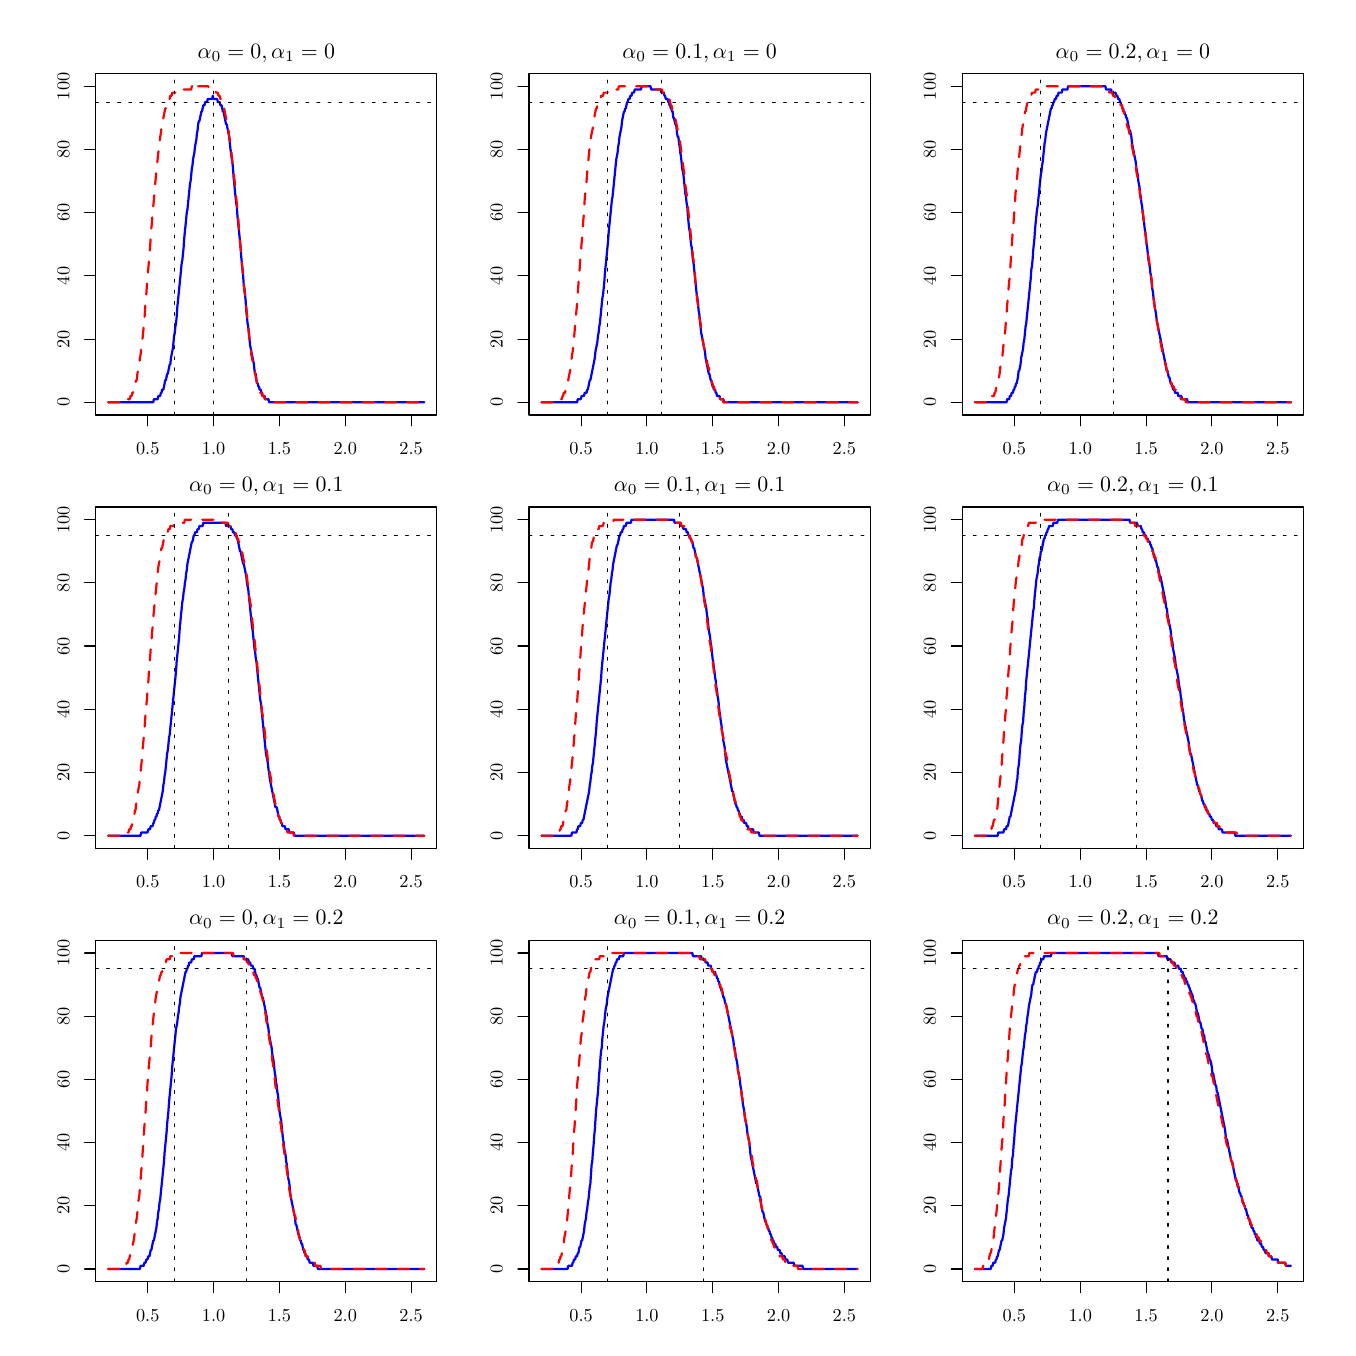
\begin{tikzpicture}[x=1pt,y=1pt]
\definecolor{fillColor}{RGB}{255,255,255}
\path[use as bounding box,fill=fillColor,fill opacity=0.00] (0,0) rectangle (469.75,469.75);
\begin{scope}
\path[clip] ( 24.55,329.80) rectangle (147.87,453.12);
\definecolor{drawColor}{RGB}{0,0,255}

\path[draw=drawColor,line width= 0.8pt,line join=round,line cap=round] ( 29.12,334.37) --
	( 29.35,334.37) --
	( 29.58,334.37) --
	( 29.81,334.37) --
	( 30.03,334.37) --
	( 30.26,334.37) --
	( 30.49,334.37) --
	( 30.72,334.37) --
	( 30.95,334.37) --
	( 31.18,334.37) --
	( 31.41,334.37) --
	( 31.64,334.37) --
	( 31.87,334.37) --
	( 32.09,334.37) --
	( 32.32,334.37) --
	( 32.55,334.37) --
	( 32.78,334.37) --
	( 33.01,334.37) --
	( 33.24,334.37) --
	( 33.47,334.37) --
	( 33.70,334.37) --
	( 33.92,334.37) --
	( 34.15,334.37) --
	( 34.38,334.37) --
	( 34.61,334.37) --
	( 34.84,334.37) --
	( 35.07,334.37) --
	( 35.30,334.37) --
	( 35.53,334.37) --
	( 35.76,334.37) --
	( 35.98,334.37) --
	( 36.21,334.37) --
	( 36.44,334.37) --
	( 36.67,334.37) --
	( 36.90,334.37) --
	( 37.13,334.37) --
	( 37.36,334.37) --
	( 37.59,334.37) --
	( 37.81,334.37) --
	( 38.04,334.37) --
	( 38.27,334.37) --
	( 38.50,334.37) --
	( 38.73,334.37) --
	( 38.96,334.37) --
	( 39.19,334.37) --
	( 39.42,334.37) --
	( 39.65,334.37) --
	( 39.87,334.37) --
	( 40.10,334.37) --
	( 40.33,334.37) --
	( 40.56,334.37) --
	( 40.79,334.37) --
	( 41.02,334.37) --
	( 41.25,334.37) --
	( 41.48,334.37) --
	( 41.71,334.37) --
	( 41.93,334.37) --
	( 42.16,334.37) --
	( 42.39,334.37) --
	( 42.62,334.37) --
	( 42.85,334.37) --
	( 43.08,334.37) --
	( 43.31,334.37) --
	( 43.54,334.37) --
	( 43.76,334.37) --
	( 43.99,334.37) --
	( 44.22,334.37) --
	( 44.45,334.37) --
	( 44.68,334.37) --
	( 44.91,334.37) --
	( 45.14,334.37) --
	( 45.37,334.37) --
	( 45.60,335.51) --
	( 45.82,335.51) --
	( 46.05,335.51) --
	( 46.28,335.51) --
	( 46.51,335.51) --
	( 46.74,335.51) --
	( 46.97,335.51) --
	( 47.20,336.65) --
	( 47.43,336.65) --
	( 47.65,336.65) --
	( 47.88,336.65) --
	( 48.11,337.80) --
	( 48.34,337.80) --
	( 48.57,338.94) --
	( 48.80,338.94) --
	( 49.03,338.94) --
	( 49.26,340.08) --
	( 49.49,341.22) --
	( 49.71,342.36) --
	( 49.94,342.36) --
	( 50.17,343.50) --
	( 50.40,344.65) --
	( 50.63,344.65) --
	( 50.86,345.79) --
	( 51.09,346.93) --
	( 51.32,348.07) --
	( 51.54,348.07) --
	( 51.77,350.36) --
	( 52.00,351.50) --
	( 52.23,352.64) --
	( 52.46,353.78) --
	( 52.69,356.06) --
	( 52.92,358.35) --
	( 53.15,359.49) --
	( 53.38,361.77) --
	( 53.60,362.92) --
	( 53.83,365.20) --
	( 54.06,368.63) --
	( 54.29,370.91) --
	( 54.52,373.19) --
	( 54.75,375.48) --
	( 54.98,377.76) --
	( 55.21,380.04) --
	( 55.43,382.33) --
	( 55.66,384.61) --
	( 55.89,385.75) --
	( 56.12,388.04) --
	( 56.35,390.32) --
	( 56.58,393.75) --
	( 56.81,396.03) --
	( 57.04,398.31) --
	( 57.27,400.60) --
	( 57.49,402.88) --
	( 57.72,404.02) --
	( 57.95,406.31) --
	( 58.18,408.59) --
	( 58.41,410.87) --
	( 58.64,413.16) --
	( 58.87,414.30) --
	( 59.10,416.58) --
	( 59.32,418.87) --
	( 59.55,420.01) --
	( 59.78,422.29) --
	( 60.01,423.43) --
	( 60.24,424.58) --
	( 60.47,426.86) --
	( 60.70,428.00) --
	( 60.93,429.14) --
	( 61.16,431.43) --
	( 61.38,432.57) --
	( 61.61,434.85) --
	( 61.84,436.00) --
	( 62.07,436.00) --
	( 62.30,437.14) --
	( 62.53,438.28) --
	( 62.76,439.42) --
	( 62.99,439.42) --
	( 63.22,440.56) --
	( 63.44,441.70) --
	( 63.67,441.70) --
	( 63.90,441.70) --
	( 64.13,442.85) --
	( 64.36,442.85) --
	( 64.59,442.85) --
	( 64.82,442.85) --
	( 65.05,443.99) --
	( 65.27,443.99) --
	( 65.50,443.99) --
	( 65.73,443.99) --
	( 65.96,443.99) --
	( 66.19,443.99) --
	( 66.42,443.99) --
	( 66.65,443.99) --
	( 66.88,445.13) --
	( 67.11,443.99) --
	( 67.33,443.99) --
	( 67.56,443.99) --
	( 67.79,443.99) --
	( 68.02,443.99) --
	( 68.25,443.99) --
	( 68.48,443.99) --
	( 68.71,442.85) --
	( 68.94,442.85) --
	( 69.16,442.85) --
	( 69.39,442.85) --
	( 69.62,441.70) --
	( 69.85,441.70) --
	( 70.08,441.70) --
	( 70.31,440.56) --
	( 70.54,439.42) --
	( 70.77,439.42) --
	( 71.00,438.28) --
	( 71.22,437.14) --
	( 71.45,436.00) --
	( 71.68,434.85) --
	( 71.91,434.85) --
	( 72.14,433.71) --
	( 72.37,432.57) --
	( 72.60,431.43) --
	( 72.83,430.29) --
	( 73.05,428.00) --
	( 73.28,425.72) --
	( 73.51,424.58) --
	( 73.74,422.29) --
	( 73.97,421.15) --
	( 74.20,418.87) --
	( 74.43,415.44) --
	( 74.66,413.16) --
	( 74.89,410.87) --
	( 75.11,408.59) --
	( 75.34,406.31) --
	( 75.57,405.16) --
	( 75.80,401.74) --
	( 76.03,399.46) --
	( 76.26,397.17) --
	( 76.49,394.89) --
	( 76.72,392.60) --
	( 76.94,390.32) --
	( 77.17,386.90) --
	( 77.40,384.61) --
	( 77.63,382.33) --
	( 77.86,380.04) --
	( 78.09,376.62) --
	( 78.32,375.48) --
	( 78.55,373.19) --
	( 78.78,370.91) --
	( 79.00,367.48) --
	( 79.23,365.20) --
	( 79.46,362.92) --
	( 79.69,361.77) --
	( 79.92,359.49) --
	( 80.15,357.21) --
	( 80.38,354.92) --
	( 80.61,353.78) --
	( 80.83,352.64) --
	( 81.06,351.50) --
	( 81.29,350.36) --
	( 81.52,349.21) --
	( 81.75,348.07) --
	( 81.98,345.79) --
	( 82.21,344.65) --
	( 82.44,344.65) --
	( 82.67,342.36) --
	( 82.89,341.22) --
	( 83.12,341.22) --
	( 83.35,340.08) --
	( 83.58,340.08) --
	( 83.81,338.94) --
	( 84.04,338.94) --
	( 84.27,338.94) --
	( 84.50,337.80) --
	( 84.73,337.80) --
	( 84.95,336.65) --
	( 85.18,336.65) --
	( 85.41,336.65) --
	( 85.64,336.65) --
	( 85.87,335.51) --
	( 86.10,335.51) --
	( 86.33,335.51) --
	( 86.56,335.51) --
	( 86.78,335.51) --
	( 87.01,335.51) --
	( 87.24,334.37) --
	( 87.47,334.37) --
	( 87.70,334.37) --
	( 87.93,334.37) --
	( 88.16,334.37) --
	( 88.39,334.37) --
	( 88.62,334.37) --
	( 88.84,334.37) --
	( 89.07,334.37) --
	( 89.30,334.37) --
	( 89.53,334.37) --
	( 89.76,334.37) --
	( 89.99,334.37) --
	( 90.22,334.37) --
	( 90.45,334.37) --
	( 90.67,334.37) --
	( 90.90,334.37) --
	( 91.13,334.37) --
	( 91.36,334.37) --
	( 91.59,334.37) --
	( 91.82,334.37) --
	( 92.05,334.37) --
	( 92.28,334.37) --
	( 92.51,334.37) --
	( 92.73,334.37) --
	( 92.96,334.37) --
	( 93.19,334.37) --
	( 93.42,334.37) --
	( 93.65,334.37) --
	( 93.88,334.37) --
	( 94.11,334.37) --
	( 94.34,334.37) --
	( 94.56,334.37) --
	( 94.79,334.37) --
	( 95.02,334.37) --
	( 95.25,334.37) --
	( 95.48,334.37) --
	( 95.71,334.37) --
	( 95.94,334.37) --
	( 96.17,334.37) --
	( 96.40,334.37) --
	( 96.62,334.37) --
	( 96.85,334.37) --
	( 97.08,334.37) --
	( 97.31,334.37) --
	( 97.54,334.37) --
	( 97.77,334.37) --
	( 98.00,334.37) --
	( 98.23,334.37) --
	( 98.45,334.37) --
	( 98.68,334.37) --
	( 98.91,334.37) --
	( 99.14,334.37) --
	( 99.37,334.37) --
	( 99.60,334.37) --
	( 99.83,334.37) --
	(100.06,334.37) --
	(100.29,334.37) --
	(100.51,334.37) --
	(100.74,334.37) --
	(100.97,334.37) --
	(101.20,334.37) --
	(101.43,334.37) --
	(101.66,334.37) --
	(101.89,334.37) --
	(102.12,334.37) --
	(102.35,334.37) --
	(102.57,334.37) --
	(102.80,334.37) --
	(103.03,334.37) --
	(103.26,334.37) --
	(103.49,334.37) --
	(103.72,334.37) --
	(103.95,334.37) --
	(104.18,334.37) --
	(104.40,334.37) --
	(104.63,334.37) --
	(104.86,334.37) --
	(105.09,334.37) --
	(105.32,334.37) --
	(105.55,334.37) --
	(105.78,334.37) --
	(106.01,334.37) --
	(106.24,334.37) --
	(106.46,334.37) --
	(106.69,334.37) --
	(106.92,334.37) --
	(107.15,334.37) --
	(107.38,334.37) --
	(107.61,334.37) --
	(107.84,334.37) --
	(108.07,334.37) --
	(108.29,334.37) --
	(108.52,334.37) --
	(108.75,334.37) --
	(108.98,334.37) --
	(109.21,334.37) --
	(109.44,334.37) --
	(109.67,334.37) --
	(109.90,334.37) --
	(110.13,334.37) --
	(110.35,334.37) --
	(110.58,334.37) --
	(110.81,334.37) --
	(111.04,334.37) --
	(111.27,334.37) --
	(111.50,334.37) --
	(111.73,334.37) --
	(111.96,334.37) --
	(112.18,334.37) --
	(112.41,334.37) --
	(112.64,334.37) --
	(112.87,334.37) --
	(113.10,334.37) --
	(113.33,334.37) --
	(113.56,334.37) --
	(113.79,334.37) --
	(114.02,334.37) --
	(114.24,334.37) --
	(114.47,334.37) --
	(114.70,334.37) --
	(114.93,334.37) --
	(115.16,334.37) --
	(115.39,334.37) --
	(115.62,334.37) --
	(115.85,334.37) --
	(116.07,334.37) --
	(116.30,334.37) --
	(116.53,334.37) --
	(116.76,334.37) --
	(116.99,334.37) --
	(117.22,334.37) --
	(117.45,334.37) --
	(117.68,334.37) --
	(117.91,334.37) --
	(118.13,334.37) --
	(118.36,334.37) --
	(118.59,334.37) --
	(118.82,334.37) --
	(119.05,334.37) --
	(119.28,334.37) --
	(119.51,334.37) --
	(119.74,334.37) --
	(119.96,334.37) --
	(120.19,334.37) --
	(120.42,334.37) --
	(120.65,334.37) --
	(120.88,334.37) --
	(121.11,334.37) --
	(121.34,334.37) --
	(121.57,334.37) --
	(121.80,334.37) --
	(122.02,334.37) --
	(122.25,334.37) --
	(122.48,334.37) --
	(122.71,334.37) --
	(122.94,334.37) --
	(123.17,334.37) --
	(123.40,334.37) --
	(123.63,334.37) --
	(123.86,334.37) --
	(124.08,334.37) --
	(124.31,334.37) --
	(124.54,334.37) --
	(124.77,334.37) --
	(125.00,334.37) --
	(125.23,334.37) --
	(125.46,334.37) --
	(125.69,334.37) --
	(125.91,334.37) --
	(126.14,334.37) --
	(126.37,334.37) --
	(126.60,334.37) --
	(126.83,334.37) --
	(127.06,334.37) --
	(127.29,334.37) --
	(127.52,334.37) --
	(127.75,334.37) --
	(127.97,334.37) --
	(128.20,334.37) --
	(128.43,334.37) --
	(128.66,334.37) --
	(128.89,334.37) --
	(129.12,334.37) --
	(129.35,334.37) --
	(129.58,334.37) --
	(129.80,334.37) --
	(130.03,334.37) --
	(130.26,334.37) --
	(130.49,334.37) --
	(130.72,334.37) --
	(130.95,334.37) --
	(131.18,334.37) --
	(131.41,334.37) --
	(131.64,334.37) --
	(131.86,334.37) --
	(132.09,334.37) --
	(132.32,334.37) --
	(132.55,334.37) --
	(132.78,334.37) --
	(133.01,334.37) --
	(133.24,334.37) --
	(133.47,334.37) --
	(133.69,334.37) --
	(133.92,334.37) --
	(134.15,334.37) --
	(134.38,334.37) --
	(134.61,334.37) --
	(134.84,334.37) --
	(135.07,334.37) --
	(135.30,334.37) --
	(135.53,334.37) --
	(135.75,334.37) --
	(135.98,334.37) --
	(136.21,334.37) --
	(136.44,334.37) --
	(136.67,334.37) --
	(136.90,334.37) --
	(137.13,334.37) --
	(137.36,334.37) --
	(137.58,334.37) --
	(137.81,334.37) --
	(138.04,334.37) --
	(138.27,334.37) --
	(138.50,334.37) --
	(138.73,334.37) --
	(138.96,334.37) --
	(139.19,334.37) --
	(139.42,334.37) --
	(139.64,334.37) --
	(139.87,334.37) --
	(140.10,334.37) --
	(140.33,334.37) --
	(140.56,334.37) --
	(140.79,334.37) --
	(141.02,334.37) --
	(141.25,334.37) --
	(141.47,334.37) --
	(141.70,334.37) --
	(141.93,334.37) --
	(142.16,334.37) --
	(142.39,334.37) --
	(142.62,334.37) --
	(142.85,334.37) --
	(143.08,334.37) --
	(143.31,334.37);
\end{scope}
\begin{scope}
\path[clip] (  0.00,  0.00) rectangle (469.75,469.75);
\definecolor{drawColor}{RGB}{0,0,0}

\path[draw=drawColor,line width= 0.4pt,line join=round,line cap=round] ( 43.39,329.80) -- (138.55,329.80);

\path[draw=drawColor,line width= 0.4pt,line join=round,line cap=round] ( 43.39,329.80) -- ( 43.39,325.84);

\path[draw=drawColor,line width= 0.4pt,line join=round,line cap=round] ( 67.18,329.80) -- ( 67.18,325.84);

\path[draw=drawColor,line width= 0.4pt,line join=round,line cap=round] ( 90.97,329.80) -- ( 90.97,325.84);

\path[draw=drawColor,line width= 0.4pt,line join=round,line cap=round] (114.76,329.80) -- (114.76,325.84);

\path[draw=drawColor,line width= 0.4pt,line join=round,line cap=round] (138.55,329.80) -- (138.55,325.84);

\node[text=drawColor,anchor=base,inner sep=0pt, outer sep=0pt, scale=  0.66] at ( 43.39,315.55) {0.5};

\node[text=drawColor,anchor=base,inner sep=0pt, outer sep=0pt, scale=  0.66] at ( 67.18,315.55) {1.0};

\node[text=drawColor,anchor=base,inner sep=0pt, outer sep=0pt, scale=  0.66] at ( 90.97,315.55) {1.5};

\node[text=drawColor,anchor=base,inner sep=0pt, outer sep=0pt, scale=  0.66] at (114.76,315.55) {2.0};

\node[text=drawColor,anchor=base,inner sep=0pt, outer sep=0pt, scale=  0.66] at (138.55,315.55) {2.5};

\path[draw=drawColor,line width= 0.4pt,line join=round,line cap=round] ( 24.55,334.37) -- ( 24.55,448.56);

\path[draw=drawColor,line width= 0.4pt,line join=round,line cap=round] ( 24.55,334.37) -- ( 20.59,334.37);

\path[draw=drawColor,line width= 0.4pt,line join=round,line cap=round] ( 24.55,357.21) -- ( 20.59,357.21);

\path[draw=drawColor,line width= 0.4pt,line join=round,line cap=round] ( 24.55,380.04) -- ( 20.59,380.04);

\path[draw=drawColor,line width= 0.4pt,line join=round,line cap=round] ( 24.55,402.88) -- ( 20.59,402.88);

\path[draw=drawColor,line width= 0.4pt,line join=round,line cap=round] ( 24.55,425.72) -- ( 20.59,425.72);

\path[draw=drawColor,line width= 0.4pt,line join=round,line cap=round] ( 24.55,448.56) -- ( 20.59,448.56);

\node[text=drawColor,rotate= 90.00,anchor=base,inner sep=0pt, outer sep=0pt, scale=  0.66] at ( 15.05,334.37) {0};

\node[text=drawColor,rotate= 90.00,anchor=base,inner sep=0pt, outer sep=0pt, scale=  0.66] at ( 15.05,357.21) {20};

\node[text=drawColor,rotate= 90.00,anchor=base,inner sep=0pt, outer sep=0pt, scale=  0.66] at ( 15.05,380.04) {40};

\node[text=drawColor,rotate= 90.00,anchor=base,inner sep=0pt, outer sep=0pt, scale=  0.66] at ( 15.05,402.88) {60};

\node[text=drawColor,rotate= 90.00,anchor=base,inner sep=0pt, outer sep=0pt, scale=  0.66] at ( 15.05,425.72) {80};

\node[text=drawColor,rotate= 90.00,anchor=base,inner sep=0pt, outer sep=0pt, scale=  0.66] at ( 15.05,448.56) {100};

\path[draw=drawColor,line width= 0.4pt,line join=round,line cap=round] ( 24.55,329.80) --
	(147.87,329.80) --
	(147.87,453.12) --
	( 24.55,453.12) --
	( 24.55,329.80);
\end{scope}
\begin{scope}
\path[clip] (  0.00,313.17) rectangle (156.58,469.75);
\definecolor{drawColor}{RGB}{0,0,0}

\node[text=drawColor,anchor=base,inner sep=0pt, outer sep=0pt, scale=  0.79] at ( 86.21,458.71) {\bfseries $\alpha_0 = 0, \alpha_1 = 0$};
\end{scope}
\begin{scope}
\path[clip] ( 24.55,329.80) rectangle (147.87,453.12);
\definecolor{drawColor}{RGB}{255,0,0}

\path[draw=drawColor,line width= 0.8pt,dash pattern=on 4pt off 4pt ,line join=round,line cap=round] ( 29.12,334.37) --
	( 29.35,334.37) --
	( 29.58,334.37) --
	( 29.81,334.37) --
	( 30.03,334.37) --
	( 30.26,334.37) --
	( 30.49,334.37) --
	( 30.72,334.37) --
	( 30.95,334.37) --
	( 31.18,334.37) --
	( 31.41,334.37) --
	( 31.64,334.37) --
	( 31.87,334.37) --
	( 32.09,334.37) --
	( 32.32,334.37) --
	( 32.55,334.37) --
	( 32.78,334.37) --
	( 33.01,334.37) --
	( 33.24,334.37) --
	( 33.47,334.37) --
	( 33.70,334.37) --
	( 33.92,334.37) --
	( 34.15,334.37) --
	( 34.38,334.37) --
	( 34.61,334.37) --
	( 34.84,334.37) --
	( 35.07,334.37) --
	( 35.30,334.37) --
	( 35.53,334.37) --
	( 35.76,334.37) --
	( 35.98,335.51) --
	( 36.21,335.51) --
	( 36.44,335.51) --
	( 36.67,335.51) --
	( 36.90,335.51) --
	( 37.13,336.65) --
	( 37.36,336.65) --
	( 37.59,336.65) --
	( 37.81,337.80) --
	( 38.04,337.80) --
	( 38.27,338.94) --
	( 38.50,338.94) --
	( 38.73,340.08) --
	( 38.96,341.22) --
	( 39.19,342.36) --
	( 39.42,342.36) --
	( 39.65,344.65) --
	( 39.87,345.79) --
	( 40.10,346.93) --
	( 40.33,348.07) --
	( 40.56,350.36) --
	( 40.79,351.50) --
	( 41.02,353.78) --
	( 41.25,354.92) --
	( 41.48,357.21) --
	( 41.71,359.49) --
	( 41.93,361.77) --
	( 42.16,364.06) --
	( 42.39,367.48) --
	( 42.62,370.91) --
	( 42.85,373.19) --
	( 43.08,376.62) --
	( 43.31,378.90) --
	( 43.54,382.33) --
	( 43.76,384.61) --
	( 43.99,388.04) --
	( 44.22,390.32) --
	( 44.45,393.75) --
	( 44.68,397.17) --
	( 44.91,399.46) --
	( 45.14,402.88) --
	( 45.37,405.16) --
	( 45.60,407.45) --
	( 45.82,410.87) --
	( 46.05,413.16) --
	( 46.28,415.44) --
	( 46.51,418.87) --
	( 46.74,420.01) --
	( 46.97,422.29) --
	( 47.20,424.58) --
	( 47.43,425.72) --
	( 47.65,428.00) --
	( 47.88,430.29) --
	( 48.11,431.43) --
	( 48.34,433.71) --
	( 48.57,434.85) --
	( 48.80,436.00) --
	( 49.03,437.14) --
	( 49.26,438.28) --
	( 49.49,439.42) --
	( 49.71,440.56) --
	( 49.94,440.56) --
	( 50.17,441.70) --
	( 50.40,441.70) --
	( 50.63,442.85) --
	( 50.86,443.99) --
	( 51.09,443.99) --
	( 51.32,443.99) --
	( 51.54,445.13) --
	( 51.77,445.13) --
	( 52.00,445.13) --
	( 52.23,446.27) --
	( 52.46,446.27) --
	( 52.69,446.27) --
	( 52.92,446.27) --
	( 53.15,446.27) --
	( 53.38,446.27) --
	( 53.60,446.27) --
	( 53.83,447.41) --
	( 54.06,447.41) --
	( 54.29,447.41) --
	( 54.52,447.41) --
	( 54.75,447.41) --
	( 54.98,447.41) --
	( 55.21,447.41) --
	( 55.43,447.41) --
	( 55.66,447.41) --
	( 55.89,447.41) --
	( 56.12,447.41) --
	( 56.35,447.41) --
	( 56.58,447.41) --
	( 56.81,447.41) --
	( 57.04,447.41) --
	( 57.27,447.41) --
	( 57.49,447.41) --
	( 57.72,447.41) --
	( 57.95,447.41) --
	( 58.18,447.41) --
	( 58.41,447.41) --
	( 58.64,447.41) --
	( 58.87,447.41) --
	( 59.10,447.41) --
	( 59.32,448.56) --
	( 59.55,448.56) --
	( 59.78,448.56) --
	( 60.01,448.56) --
	( 60.24,448.56) --
	( 60.47,448.56) --
	( 60.70,447.41) --
	( 60.93,447.41) --
	( 61.16,447.41) --
	( 61.38,447.41) --
	( 61.61,448.56) --
	( 61.84,448.56) --
	( 62.07,448.56) --
	( 62.30,448.56) --
	( 62.53,448.56) --
	( 62.76,448.56) --
	( 62.99,448.56) --
	( 63.22,448.56) --
	( 63.44,448.56) --
	( 63.67,448.56) --
	( 63.90,448.56) --
	( 64.13,448.56) --
	( 64.36,448.56) --
	( 64.59,448.56) --
	( 64.82,448.56) --
	( 65.05,448.56) --
	( 65.27,448.56) --
	( 65.50,447.41) --
	( 65.73,447.41) --
	( 65.96,447.41) --
	( 66.19,447.41) --
	( 66.42,447.41) --
	( 66.65,447.41) --
	( 66.88,447.41) --
	( 67.11,447.41) --
	( 67.33,447.41) --
	( 67.56,447.41) --
	( 67.79,447.41) --
	( 68.02,446.27) --
	( 68.25,446.27) --
	( 68.48,446.27) --
	( 68.71,446.27) --
	( 68.94,445.13) --
	( 69.16,445.13) --
	( 69.39,445.13) --
	( 69.62,443.99) --
	( 69.85,443.99) --
	( 70.08,442.85) --
	( 70.31,441.70) --
	( 70.54,441.70) --
	( 70.77,440.56) --
	( 71.00,440.56) --
	( 71.22,439.42) --
	( 71.45,438.28) --
	( 71.68,437.14) --
	( 71.91,436.00) --
	( 72.14,434.85) --
	( 72.37,433.71) --
	( 72.60,432.57) --
	( 72.83,430.29) --
	( 73.05,429.14) --
	( 73.28,428.00) --
	( 73.51,425.72) --
	( 73.74,423.43) --
	( 73.97,421.15) --
	( 74.20,420.01) --
	( 74.43,417.73) --
	( 74.66,415.44) --
	( 74.89,413.16) --
	( 75.11,410.87) --
	( 75.34,408.59) --
	( 75.57,406.31) --
	( 75.80,404.02) --
	( 76.03,401.74) --
	( 76.26,398.31) --
	( 76.49,394.89) --
	( 76.72,392.60) --
	( 76.94,390.32) --
	( 77.17,388.04) --
	( 77.40,384.61) --
	( 77.63,382.33) --
	( 77.86,380.04) --
	( 78.09,377.76) --
	( 78.32,374.33) --
	( 78.55,373.19) --
	( 78.78,370.91) --
	( 79.00,368.63) --
	( 79.23,366.34) --
	( 79.46,364.06) --
	( 79.69,361.77) --
	( 79.92,359.49) --
	( 80.15,357.21) --
	( 80.38,354.92) --
	( 80.61,353.78) --
	( 80.83,351.50) --
	( 81.06,350.36) --
	( 81.29,349.21) --
	( 81.52,348.07) --
	( 81.75,346.93) --
	( 81.98,345.79) --
	( 82.21,344.65) --
	( 82.44,343.50) --
	( 82.67,342.36) --
	( 82.89,341.22) --
	( 83.12,341.22) --
	( 83.35,340.08) --
	( 83.58,338.94) --
	( 83.81,338.94) --
	( 84.04,337.80) --
	( 84.27,337.80) --
	( 84.50,337.80) --
	( 84.73,336.65) --
	( 84.95,336.65) --
	( 85.18,336.65) --
	( 85.41,336.65) --
	( 85.64,335.51) --
	( 85.87,335.51) --
	( 86.10,335.51) --
	( 86.33,335.51) --
	( 86.56,335.51) --
	( 86.78,335.51) --
	( 87.01,335.51) --
	( 87.24,335.51) --
	( 87.47,335.51) --
	( 87.70,334.37) --
	( 87.93,334.37) --
	( 88.16,334.37) --
	( 88.39,334.37) --
	( 88.62,334.37) --
	( 88.84,334.37) --
	( 89.07,334.37) --
	( 89.30,334.37) --
	( 89.53,334.37) --
	( 89.76,334.37) --
	( 89.99,334.37) --
	( 90.22,334.37) --
	( 90.45,334.37) --
	( 90.67,334.37) --
	( 90.90,334.37) --
	( 91.13,334.37) --
	( 91.36,334.37) --
	( 91.59,334.37) --
	( 91.82,334.37) --
	( 92.05,334.37) --
	( 92.28,334.37) --
	( 92.51,334.37) --
	( 92.73,334.37) --
	( 92.96,334.37) --
	( 93.19,334.37) --
	( 93.42,334.37) --
	( 93.65,334.37) --
	( 93.88,334.37) --
	( 94.11,334.37) --
	( 94.34,334.37) --
	( 94.56,334.37) --
	( 94.79,334.37) --
	( 95.02,334.37) --
	( 95.25,334.37) --
	( 95.48,334.37) --
	( 95.71,334.37) --
	( 95.94,334.37) --
	( 96.17,334.37) --
	( 96.40,334.37) --
	( 96.62,334.37) --
	( 96.85,334.37) --
	( 97.08,334.37) --
	( 97.31,334.37) --
	( 97.54,334.37) --
	( 97.77,334.37) --
	( 98.00,334.37) --
	( 98.23,334.37) --
	( 98.45,334.37) --
	( 98.68,334.37) --
	( 98.91,334.37) --
	( 99.14,334.37) --
	( 99.37,334.37) --
	( 99.60,334.37) --
	( 99.83,334.37) --
	(100.06,334.37) --
	(100.29,334.37) --
	(100.51,334.37) --
	(100.74,334.37) --
	(100.97,334.37) --
	(101.20,334.37) --
	(101.43,334.37) --
	(101.66,334.37) --
	(101.89,334.37) --
	(102.12,334.37) --
	(102.35,334.37) --
	(102.57,334.37) --
	(102.80,334.37) --
	(103.03,334.37) --
	(103.26,334.37) --
	(103.49,334.37) --
	(103.72,334.37) --
	(103.95,334.37) --
	(104.18,334.37) --
	(104.40,334.37) --
	(104.63,334.37) --
	(104.86,334.37) --
	(105.09,334.37) --
	(105.32,334.37) --
	(105.55,334.37) --
	(105.78,334.37) --
	(106.01,334.37) --
	(106.24,334.37) --
	(106.46,334.37) --
	(106.69,334.37) --
	(106.92,334.37) --
	(107.15,334.37) --
	(107.38,334.37) --
	(107.61,334.37) --
	(107.84,334.37) --
	(108.07,334.37) --
	(108.29,334.37) --
	(108.52,334.37) --
	(108.75,334.37) --
	(108.98,334.37) --
	(109.21,334.37) --
	(109.44,334.37) --
	(109.67,334.37) --
	(109.90,334.37) --
	(110.13,334.37) --
	(110.35,334.37) --
	(110.58,334.37) --
	(110.81,334.37) --
	(111.04,334.37) --
	(111.27,334.37) --
	(111.50,334.37) --
	(111.73,334.37) --
	(111.96,334.37) --
	(112.18,334.37) --
	(112.41,334.37) --
	(112.64,334.37) --
	(112.87,334.37) --
	(113.10,334.37) --
	(113.33,334.37) --
	(113.56,334.37) --
	(113.79,334.37) --
	(114.02,334.37) --
	(114.24,334.37) --
	(114.47,334.37) --
	(114.70,334.37) --
	(114.93,334.37) --
	(115.16,334.37) --
	(115.39,334.37) --
	(115.62,334.37) --
	(115.85,334.37) --
	(116.07,334.37) --
	(116.30,334.37) --
	(116.53,334.37) --
	(116.76,334.37) --
	(116.99,334.37) --
	(117.22,334.37) --
	(117.45,334.37) --
	(117.68,334.37) --
	(117.91,334.37) --
	(118.13,334.37) --
	(118.36,334.37) --
	(118.59,334.37) --
	(118.82,334.37) --
	(119.05,334.37) --
	(119.28,334.37) --
	(119.51,334.37) --
	(119.74,334.37) --
	(119.96,334.37) --
	(120.19,334.37) --
	(120.42,334.37) --
	(120.65,334.37) --
	(120.88,334.37) --
	(121.11,334.37) --
	(121.34,334.37) --
	(121.57,334.37) --
	(121.80,334.37) --
	(122.02,334.37) --
	(122.25,334.37) --
	(122.48,334.37) --
	(122.71,334.37) --
	(122.94,334.37) --
	(123.17,334.37) --
	(123.40,334.37) --
	(123.63,334.37) --
	(123.86,334.37) --
	(124.08,334.37) --
	(124.31,334.37) --
	(124.54,334.37) --
	(124.77,334.37) --
	(125.00,334.37) --
	(125.23,334.37) --
	(125.46,334.37) --
	(125.69,334.37) --
	(125.91,334.37) --
	(126.14,334.37) --
	(126.37,334.37) --
	(126.60,334.37) --
	(126.83,334.37) --
	(127.06,334.37) --
	(127.29,334.37) --
	(127.52,334.37) --
	(127.75,334.37) --
	(127.97,334.37) --
	(128.20,334.37) --
	(128.43,334.37) --
	(128.66,334.37) --
	(128.89,334.37) --
	(129.12,334.37) --
	(129.35,334.37) --
	(129.58,334.37) --
	(129.80,334.37) --
	(130.03,334.37) --
	(130.26,334.37) --
	(130.49,334.37) --
	(130.72,334.37) --
	(130.95,334.37) --
	(131.18,334.37) --
	(131.41,334.37) --
	(131.64,334.37) --
	(131.86,334.37) --
	(132.09,334.37) --
	(132.32,334.37) --
	(132.55,334.37) --
	(132.78,334.37) --
	(133.01,334.37) --
	(133.24,334.37) --
	(133.47,334.37) --
	(133.69,334.37) --
	(133.92,334.37) --
	(134.15,334.37) --
	(134.38,334.37) --
	(134.61,334.37) --
	(134.84,334.37) --
	(135.07,334.37) --
	(135.30,334.37) --
	(135.53,334.37) --
	(135.75,334.37) --
	(135.98,334.37) --
	(136.21,334.37) --
	(136.44,334.37) --
	(136.67,334.37) --
	(136.90,334.37) --
	(137.13,334.37) --
	(137.36,334.37) --
	(137.58,334.37) --
	(137.81,334.37) --
	(138.04,334.37) --
	(138.27,334.37) --
	(138.50,334.37) --
	(138.73,334.37) --
	(138.96,334.37) --
	(139.19,334.37) --
	(139.42,334.37) --
	(139.64,334.37) --
	(139.87,334.37) --
	(140.10,334.37) --
	(140.33,334.37) --
	(140.56,334.37) --
	(140.79,334.37) --
	(141.02,334.37) --
	(141.25,334.37) --
	(141.47,334.37) --
	(141.70,334.37) --
	(141.93,334.37) --
	(142.16,334.37) --
	(142.39,334.37) --
	(142.62,334.37) --
	(142.85,334.37) --
	(143.08,334.37) --
	(143.31,334.37);
\definecolor{drawColor}{RGB}{0,0,0}

\path[draw=drawColor,line width= 0.4pt,dash pattern=on 1pt off 3pt ,line join=round,line cap=round] ( 24.55,442.85) -- (147.87,442.85);

\path[draw=drawColor,line width= 0.4pt,dash pattern=on 1pt off 3pt ,line join=round,line cap=round] ( 52.91,329.80) -- ( 52.91,453.12);

\path[draw=drawColor,line width= 0.4pt,dash pattern=on 1pt off 3pt ,line join=round,line cap=round] ( 67.18,329.80) -- ( 67.18,453.12);
\end{scope}
\begin{scope}
\path[clip] (181.14,329.80) rectangle (304.46,453.12);
\definecolor{drawColor}{RGB}{0,0,255}

\path[draw=drawColor,line width= 0.8pt,line join=round,line cap=round] (185.70,334.37) --
	(185.93,334.37) --
	(186.16,334.37) --
	(186.39,334.37) --
	(186.62,334.37) --
	(186.85,334.37) --
	(187.08,334.37) --
	(187.31,334.37) --
	(187.54,334.37) --
	(187.76,334.37) --
	(187.99,334.37) --
	(188.22,334.37) --
	(188.45,334.37) --
	(188.68,334.37) --
	(188.91,334.37) --
	(189.14,334.37) --
	(189.37,334.37) --
	(189.59,334.37) --
	(189.82,334.37) --
	(190.05,334.37) --
	(190.28,334.37) --
	(190.51,334.37) --
	(190.74,334.37) --
	(190.97,334.37) --
	(191.20,334.37) --
	(191.43,334.37) --
	(191.65,334.37) --
	(191.88,334.37) --
	(192.11,334.37) --
	(192.34,334.37) --
	(192.57,334.37) --
	(192.80,334.37) --
	(193.03,334.37) --
	(193.26,334.37) --
	(193.48,334.37) --
	(193.71,334.37) --
	(193.94,334.37) --
	(194.17,334.37) --
	(194.40,334.37) --
	(194.63,334.37) --
	(194.86,334.37) --
	(195.09,334.37) --
	(195.32,334.37) --
	(195.54,334.37) --
	(195.77,334.37) --
	(196.00,334.37) --
	(196.23,334.37) --
	(196.46,334.37) --
	(196.69,334.37) --
	(196.92,334.37) --
	(197.15,334.37) --
	(197.37,334.37) --
	(197.60,334.37) --
	(197.83,334.37) --
	(198.06,334.37) --
	(198.29,334.37) --
	(198.52,334.37) --
	(198.75,335.51) --
	(198.98,335.51) --
	(199.21,335.51) --
	(199.43,335.51) --
	(199.66,335.51) --
	(199.89,335.51) --
	(200.12,336.65) --
	(200.35,336.65) --
	(200.58,336.65) --
	(200.81,336.65) --
	(201.04,336.65) --
	(201.26,337.80) --
	(201.49,337.80) --
	(201.72,337.80) --
	(201.95,337.80) --
	(202.18,338.94) --
	(202.41,338.94) --
	(202.64,340.08) --
	(202.87,341.22) --
	(203.10,342.36) --
	(203.32,342.36) --
	(203.55,343.50) --
	(203.78,344.65) --
	(204.01,345.79) --
	(204.24,346.93) --
	(204.47,348.07) --
	(204.70,349.21) --
	(204.93,350.36) --
	(205.15,352.64) --
	(205.38,353.78) --
	(205.61,354.92) --
	(205.84,356.06) --
	(206.07,358.35) --
	(206.30,359.49) --
	(206.53,361.77) --
	(206.76,362.92) --
	(206.99,365.20) --
	(207.21,367.48) --
	(207.44,369.77) --
	(207.67,372.05) --
	(207.90,373.19) --
	(208.13,375.48) --
	(208.36,377.76) --
	(208.59,381.19) --
	(208.82,383.47) --
	(209.05,385.75) --
	(209.27,388.04) --
	(209.50,390.32) --
	(209.73,392.60) --
	(209.96,396.03) --
	(210.19,398.31) --
	(210.42,400.60) --
	(210.65,402.88) --
	(210.88,405.16) --
	(211.10,407.45) --
	(211.33,408.59) --
	(211.56,410.87) --
	(211.79,413.16) --
	(212.02,415.44) --
	(212.25,417.73) --
	(212.48,420.01) --
	(212.71,422.29) --
	(212.94,423.43) --
	(213.16,424.58) --
	(213.39,426.86) --
	(213.62,428.00) --
	(213.85,430.29) --
	(214.08,431.43) --
	(214.31,432.57) --
	(214.54,433.71) --
	(214.77,436.00) --
	(214.99,437.14) --
	(215.22,438.28) --
	(215.45,439.42) --
	(215.68,439.42) --
	(215.91,440.56) --
	(216.14,440.56) --
	(216.37,441.70) --
	(216.60,442.85) --
	(216.83,442.85) --
	(217.05,443.99) --
	(217.28,443.99) --
	(217.51,443.99) --
	(217.74,445.13) --
	(217.97,445.13) --
	(218.20,445.13) --
	(218.43,446.27) --
	(218.66,446.27) --
	(218.88,446.27) --
	(219.11,446.27) --
	(219.34,447.41) --
	(219.57,447.41) --
	(219.80,447.41) --
	(220.03,447.41) --
	(220.26,447.41) --
	(220.49,447.41) --
	(220.72,447.41) --
	(220.94,447.41) --
	(221.17,447.41) --
	(221.40,447.41) --
	(221.63,447.41) --
	(221.86,448.56) --
	(222.09,448.56) --
	(222.32,448.56) --
	(222.55,448.56) --
	(222.77,448.56) --
	(223.00,448.56) --
	(223.23,448.56) --
	(223.46,448.56) --
	(223.69,448.56) --
	(223.92,448.56) --
	(224.15,448.56) --
	(224.38,448.56) --
	(224.61,448.56) --
	(224.83,448.56) --
	(225.06,448.56) --
	(225.29,447.41) --
	(225.52,447.41) --
	(225.75,447.41) --
	(225.98,447.41) --
	(226.21,447.41) --
	(226.44,447.41) --
	(226.66,447.41) --
	(226.89,447.41) --
	(227.12,447.41) --
	(227.35,447.41) --
	(227.58,447.41) --
	(227.81,447.41) --
	(228.04,447.41) --
	(228.27,447.41) --
	(228.50,447.41) --
	(228.72,447.41) --
	(228.95,446.27) --
	(229.18,446.27) --
	(229.41,446.27) --
	(229.64,446.27) --
	(229.87,446.27) --
	(230.10,445.13) --
	(230.33,445.13) --
	(230.56,443.99) --
	(230.78,443.99) --
	(231.01,443.99) --
	(231.24,443.99) --
	(231.47,442.85) --
	(231.70,442.85) --
	(231.93,441.70) --
	(232.16,441.70) --
	(232.39,440.56) --
	(232.61,440.56) --
	(232.84,439.42) --
	(233.07,439.42) --
	(233.30,437.14) --
	(233.53,437.14) --
	(233.76,436.00) --
	(233.99,434.85) --
	(234.22,434.85) --
	(234.45,433.71) --
	(234.67,431.43) --
	(234.90,430.29) --
	(235.13,430.29) --
	(235.36,428.00) --
	(235.59,426.86) --
	(235.82,424.58) --
	(236.05,423.43) --
	(236.28,421.15) --
	(236.50,418.87) --
	(236.73,417.73) --
	(236.96,416.58) --
	(237.19,414.30) --
	(237.42,412.02) --
	(237.65,409.73) --
	(237.88,408.59) --
	(238.11,406.31) --
	(238.34,405.16) --
	(238.56,401.74) --
	(238.79,399.46) --
	(239.02,397.17) --
	(239.25,396.03) --
	(239.48,393.75) --
	(239.71,391.46) --
	(239.94,390.32) --
	(240.17,388.04) --
	(240.39,385.75) --
	(240.62,384.61) --
	(240.85,382.33) --
	(241.08,380.04) --
	(241.31,377.76) --
	(241.54,375.48) --
	(241.77,373.19) --
	(242.00,372.05) --
	(242.23,369.77) --
	(242.45,367.48) --
	(242.68,366.34) --
	(242.91,364.06) --
	(243.14,361.77) --
	(243.37,359.49) --
	(243.60,358.35) --
	(243.83,357.21) --
	(244.06,356.06) --
	(244.28,354.92) --
	(244.51,353.78) --
	(244.74,352.64) --
	(244.97,350.36) --
	(245.20,349.21) --
	(245.43,348.07) --
	(245.66,346.93) --
	(245.89,345.79) --
	(246.12,344.65) --
	(246.34,344.65) --
	(246.57,343.50) --
	(246.80,342.36) --
	(247.03,342.36) --
	(247.26,341.22) --
	(247.49,340.08) --
	(247.72,340.08) --
	(247.95,338.94) --
	(248.18,338.94) --
	(248.40,338.94) --
	(248.63,337.80) --
	(248.86,337.80) --
	(249.09,336.65) --
	(249.32,336.65) --
	(249.55,336.65) --
	(249.78,336.65) --
	(250.01,336.65) --
	(250.23,335.51) --
	(250.46,335.51) --
	(250.69,335.51) --
	(250.92,335.51) --
	(251.15,335.51) --
	(251.38,335.51) --
	(251.61,334.37) --
	(251.84,334.37) --
	(252.07,334.37) --
	(252.29,334.37) --
	(252.52,334.37) --
	(252.75,334.37) --
	(252.98,334.37) --
	(253.21,334.37) --
	(253.44,334.37) --
	(253.67,334.37) --
	(253.90,334.37) --
	(254.12,334.37) --
	(254.35,334.37) --
	(254.58,334.37) --
	(254.81,334.37) --
	(255.04,334.37) --
	(255.27,334.37) --
	(255.50,334.37) --
	(255.73,334.37) --
	(255.96,334.37) --
	(256.18,334.37) --
	(256.41,334.37) --
	(256.64,334.37) --
	(256.87,334.37) --
	(257.10,334.37) --
	(257.33,334.37) --
	(257.56,334.37) --
	(257.79,334.37) --
	(258.01,334.37) --
	(258.24,334.37) --
	(258.47,334.37) --
	(258.70,334.37) --
	(258.93,334.37) --
	(259.16,334.37) --
	(259.39,334.37) --
	(259.62,334.37) --
	(259.85,334.37) --
	(260.07,334.37) --
	(260.30,334.37) --
	(260.53,334.37) --
	(260.76,334.37) --
	(260.99,334.37) --
	(261.22,334.37) --
	(261.45,334.37) --
	(261.68,334.37) --
	(261.90,334.37) --
	(262.13,334.37) --
	(262.36,334.37) --
	(262.59,334.37) --
	(262.82,334.37) --
	(263.05,334.37) --
	(263.28,334.37) --
	(263.51,334.37) --
	(263.74,334.37) --
	(263.96,334.37) --
	(264.19,334.37) --
	(264.42,334.37) --
	(264.65,334.37) --
	(264.88,334.37) --
	(265.11,334.37) --
	(265.34,334.37) --
	(265.57,334.37) --
	(265.79,334.37) --
	(266.02,334.37) --
	(266.25,334.37) --
	(266.48,334.37) --
	(266.71,334.37) --
	(266.94,334.37) --
	(267.17,334.37) --
	(267.40,334.37) --
	(267.63,334.37) --
	(267.85,334.37) --
	(268.08,334.37) --
	(268.31,334.37) --
	(268.54,334.37) --
	(268.77,334.37) --
	(269.00,334.37) --
	(269.23,334.37) --
	(269.46,334.37) --
	(269.69,334.37) --
	(269.91,334.37) --
	(270.14,334.37) --
	(270.37,334.37) --
	(270.60,334.37) --
	(270.83,334.37) --
	(271.06,334.37) --
	(271.29,334.37) --
	(271.52,334.37) --
	(271.74,334.37) --
	(271.97,334.37) --
	(272.20,334.37) --
	(272.43,334.37) --
	(272.66,334.37) --
	(272.89,334.37) --
	(273.12,334.37) --
	(273.35,334.37) --
	(273.58,334.37) --
	(273.80,334.37) --
	(274.03,334.37) --
	(274.26,334.37) --
	(274.49,334.37) --
	(274.72,334.37) --
	(274.95,334.37) --
	(275.18,334.37) --
	(275.41,334.37) --
	(275.63,334.37) --
	(275.86,334.37) --
	(276.09,334.37) --
	(276.32,334.37) --
	(276.55,334.37) --
	(276.78,334.37) --
	(277.01,334.37) --
	(277.24,334.37) --
	(277.47,334.37) --
	(277.69,334.37) --
	(277.92,334.37) --
	(278.15,334.37) --
	(278.38,334.37) --
	(278.61,334.37) --
	(278.84,334.37) --
	(279.07,334.37) --
	(279.30,334.37) --
	(279.52,334.37) --
	(279.75,334.37) --
	(279.98,334.37) --
	(280.21,334.37) --
	(280.44,334.37) --
	(280.67,334.37) --
	(280.90,334.37) --
	(281.13,334.37) --
	(281.36,334.37) --
	(281.58,334.37) --
	(281.81,334.37) --
	(282.04,334.37) --
	(282.27,334.37) --
	(282.50,334.37) --
	(282.73,334.37) --
	(282.96,334.37) --
	(283.19,334.37) --
	(283.41,334.37) --
	(283.64,334.37) --
	(283.87,334.37) --
	(284.10,334.37) --
	(284.33,334.37) --
	(284.56,334.37) --
	(284.79,334.37) --
	(285.02,334.37) --
	(285.25,334.37) --
	(285.47,334.37) --
	(285.70,334.37) --
	(285.93,334.37) --
	(286.16,334.37) --
	(286.39,334.37) --
	(286.62,334.37) --
	(286.85,334.37) --
	(287.08,334.37) --
	(287.30,334.37) --
	(287.53,334.37) --
	(287.76,334.37) --
	(287.99,334.37) --
	(288.22,334.37) --
	(288.45,334.37) --
	(288.68,334.37) --
	(288.91,334.37) --
	(289.14,334.37) --
	(289.36,334.37) --
	(289.59,334.37) --
	(289.82,334.37) --
	(290.05,334.37) --
	(290.28,334.37) --
	(290.51,334.37) --
	(290.74,334.37) --
	(290.97,334.37) --
	(291.20,334.37) --
	(291.42,334.37) --
	(291.65,334.37) --
	(291.88,334.37) --
	(292.11,334.37) --
	(292.34,334.37) --
	(292.57,334.37) --
	(292.80,334.37) --
	(293.03,334.37) --
	(293.25,334.37) --
	(293.48,334.37) --
	(293.71,334.37) --
	(293.94,334.37) --
	(294.17,334.37) --
	(294.40,334.37) --
	(294.63,334.37) --
	(294.86,334.37) --
	(295.09,334.37) --
	(295.31,334.37) --
	(295.54,334.37) --
	(295.77,334.37) --
	(296.00,334.37) --
	(296.23,334.37) --
	(296.46,334.37) --
	(296.69,334.37) --
	(296.92,334.37) --
	(297.14,334.37) --
	(297.37,334.37) --
	(297.60,334.37) --
	(297.83,334.37) --
	(298.06,334.37) --
	(298.29,334.37) --
	(298.52,334.37) --
	(298.75,334.37) --
	(298.98,334.37) --
	(299.20,334.37) --
	(299.43,334.37) --
	(299.66,334.37) --
	(299.89,334.37);
\end{scope}
\begin{scope}
\path[clip] (  0.00,  0.00) rectangle (469.75,469.75);
\definecolor{drawColor}{RGB}{0,0,0}

\path[draw=drawColor,line width= 0.4pt,line join=round,line cap=round] (199.98,329.80) -- (295.13,329.80);

\path[draw=drawColor,line width= 0.4pt,line join=round,line cap=round] (199.98,329.80) -- (199.98,325.84);

\path[draw=drawColor,line width= 0.4pt,line join=round,line cap=round] (223.77,329.80) -- (223.77,325.84);

\path[draw=drawColor,line width= 0.4pt,line join=round,line cap=round] (247.56,329.80) -- (247.56,325.84);

\path[draw=drawColor,line width= 0.4pt,line join=round,line cap=round] (271.34,329.80) -- (271.34,325.84);

\path[draw=drawColor,line width= 0.4pt,line join=round,line cap=round] (295.13,329.80) -- (295.13,325.84);

\node[text=drawColor,anchor=base,inner sep=0pt, outer sep=0pt, scale=  0.66] at (199.98,315.55) {0.5};

\node[text=drawColor,anchor=base,inner sep=0pt, outer sep=0pt, scale=  0.66] at (223.77,315.55) {1.0};

\node[text=drawColor,anchor=base,inner sep=0pt, outer sep=0pt, scale=  0.66] at (247.56,315.55) {1.5};

\node[text=drawColor,anchor=base,inner sep=0pt, outer sep=0pt, scale=  0.66] at (271.34,315.55) {2.0};

\node[text=drawColor,anchor=base,inner sep=0pt, outer sep=0pt, scale=  0.66] at (295.13,315.55) {2.5};

\path[draw=drawColor,line width= 0.4pt,line join=round,line cap=round] (181.14,334.37) -- (181.14,448.56);

\path[draw=drawColor,line width= 0.4pt,line join=round,line cap=round] (181.14,334.37) -- (177.18,334.37);

\path[draw=drawColor,line width= 0.4pt,line join=round,line cap=round] (181.14,357.21) -- (177.18,357.21);

\path[draw=drawColor,line width= 0.4pt,line join=round,line cap=round] (181.14,380.04) -- (177.18,380.04);

\path[draw=drawColor,line width= 0.4pt,line join=round,line cap=round] (181.14,402.88) -- (177.18,402.88);

\path[draw=drawColor,line width= 0.4pt,line join=round,line cap=round] (181.14,425.72) -- (177.18,425.72);

\path[draw=drawColor,line width= 0.4pt,line join=round,line cap=round] (181.14,448.56) -- (177.18,448.56);

\node[text=drawColor,rotate= 90.00,anchor=base,inner sep=0pt, outer sep=0pt, scale=  0.66] at (171.63,334.37) {0};

\node[text=drawColor,rotate= 90.00,anchor=base,inner sep=0pt, outer sep=0pt, scale=  0.66] at (171.63,357.21) {20};

\node[text=drawColor,rotate= 90.00,anchor=base,inner sep=0pt, outer sep=0pt, scale=  0.66] at (171.63,380.04) {40};

\node[text=drawColor,rotate= 90.00,anchor=base,inner sep=0pt, outer sep=0pt, scale=  0.66] at (171.63,402.88) {60};

\node[text=drawColor,rotate= 90.00,anchor=base,inner sep=0pt, outer sep=0pt, scale=  0.66] at (171.63,425.72) {80};

\node[text=drawColor,rotate= 90.00,anchor=base,inner sep=0pt, outer sep=0pt, scale=  0.66] at (171.63,448.56) {100};

\path[draw=drawColor,line width= 0.4pt,line join=round,line cap=round] (181.14,329.80) --
	(304.46,329.80) --
	(304.46,453.12) --
	(181.14,453.12) --
	(181.14,329.80);
\end{scope}
\begin{scope}
\path[clip] (156.58,313.17) rectangle (313.17,469.75);
\definecolor{drawColor}{RGB}{0,0,0}

\node[text=drawColor,anchor=base,inner sep=0pt, outer sep=0pt, scale=  0.79] at (242.80,458.71) {\bfseries $\alpha_0 = 0.1, \alpha_1 = 0$};
\end{scope}
\begin{scope}
\path[clip] (181.14,329.80) rectangle (304.46,453.12);
\definecolor{drawColor}{RGB}{255,0,0}

\path[draw=drawColor,line width= 0.8pt,dash pattern=on 4pt off 4pt ,line join=round,line cap=round] (185.70,334.37) --
	(185.93,334.37) --
	(186.16,334.37) --
	(186.39,334.37) --
	(186.62,334.37) --
	(186.85,334.37) --
	(187.08,334.37) --
	(187.31,334.37) --
	(187.54,334.37) --
	(187.76,334.37) --
	(187.99,334.37) --
	(188.22,334.37) --
	(188.45,334.37) --
	(188.68,334.37) --
	(188.91,334.37) --
	(189.14,334.37) --
	(189.37,334.37) --
	(189.59,334.37) --
	(189.82,334.37) --
	(190.05,334.37) --
	(190.28,334.37) --
	(190.51,334.37) --
	(190.74,334.37) --
	(190.97,334.37) --
	(191.20,334.37) --
	(191.43,335.51) --
	(191.65,335.51) --
	(191.88,335.51) --
	(192.11,335.51) --
	(192.34,335.51) --
	(192.57,335.51) --
	(192.80,335.51) --
	(193.03,335.51) --
	(193.26,336.65) --
	(193.48,336.65) --
	(193.71,337.80) --
	(193.94,337.80) --
	(194.17,337.80) --
	(194.40,338.94) --
	(194.63,340.08) --
	(194.86,341.22) --
	(195.09,341.22) --
	(195.32,342.36) --
	(195.54,343.50) --
	(195.77,344.65) --
	(196.00,345.79) --
	(196.23,346.93) --
	(196.46,349.21) --
	(196.69,351.50) --
	(196.92,352.64) --
	(197.15,354.92) --
	(197.37,357.21) --
	(197.60,359.49) --
	(197.83,362.92) --
	(198.06,365.20) --
	(198.29,367.48) --
	(198.52,369.77) --
	(198.75,373.19) --
	(198.98,376.62) --
	(199.21,380.04) --
	(199.43,382.33) --
	(199.66,385.75) --
	(199.89,388.04) --
	(200.12,391.46) --
	(200.35,393.75) --
	(200.58,397.17) --
	(200.81,400.60) --
	(201.04,402.88) --
	(201.26,407.45) --
	(201.49,409.73) --
	(201.72,412.02) --
	(201.95,414.30) --
	(202.18,417.73) --
	(202.41,420.01) --
	(202.64,422.29) --
	(202.87,424.58) --
	(203.10,426.86) --
	(203.32,428.00) --
	(203.55,430.29) --
	(203.78,431.43) --
	(204.01,432.57) --
	(204.24,433.71) --
	(204.47,436.00) --
	(204.70,437.14) --
	(204.93,438.28) --
	(205.15,439.42) --
	(205.38,440.56) --
	(205.61,440.56) --
	(205.84,441.70) --
	(206.07,441.70) --
	(206.30,442.85) --
	(206.53,443.99) --
	(206.76,443.99) --
	(206.99,443.99) --
	(207.21,445.13) --
	(207.44,445.13) --
	(207.67,445.13) --
	(207.90,445.13) --
	(208.13,446.27) --
	(208.36,446.27) --
	(208.59,446.27) --
	(208.82,446.27) --
	(209.05,446.27) --
	(209.27,446.27) --
	(209.50,446.27) --
	(209.73,447.41) --
	(209.96,447.41) --
	(210.19,447.41) --
	(210.42,447.41) --
	(210.65,447.41) --
	(210.88,447.41) --
	(211.10,447.41) --
	(211.33,447.41) --
	(211.56,447.41) --
	(211.79,447.41) --
	(212.02,447.41) --
	(212.25,447.41) --
	(212.48,447.41) --
	(212.71,447.41) --
	(212.94,447.41) --
	(213.16,447.41) --
	(213.39,447.41) --
	(213.62,448.56) --
	(213.85,448.56) --
	(214.08,448.56) --
	(214.31,448.56) --
	(214.54,448.56) --
	(214.77,448.56) --
	(214.99,448.56) --
	(215.22,448.56) --
	(215.45,448.56) --
	(215.68,448.56) --
	(215.91,448.56) --
	(216.14,448.56) --
	(216.37,448.56) --
	(216.60,448.56) --
	(216.83,448.56) --
	(217.05,448.56) --
	(217.28,448.56) --
	(217.51,448.56) --
	(217.74,448.56) --
	(217.97,448.56) --
	(218.20,448.56) --
	(218.43,448.56) --
	(218.66,448.56) --
	(218.88,448.56) --
	(219.11,448.56) --
	(219.34,448.56) --
	(219.57,448.56) --
	(219.80,448.56) --
	(220.03,448.56) --
	(220.26,448.56) --
	(220.49,448.56) --
	(220.72,448.56) --
	(220.94,448.56) --
	(221.17,448.56) --
	(221.40,448.56) --
	(221.63,448.56) --
	(221.86,448.56) --
	(222.09,448.56) --
	(222.32,448.56) --
	(222.55,448.56) --
	(222.77,448.56) --
	(223.00,448.56) --
	(223.23,448.56) --
	(223.46,448.56) --
	(223.69,448.56) --
	(223.92,448.56) --
	(224.15,448.56) --
	(224.38,448.56) --
	(224.61,448.56) --
	(224.83,447.41) --
	(225.06,447.41) --
	(225.29,447.41) --
	(225.52,447.41) --
	(225.75,447.41) --
	(225.98,447.41) --
	(226.21,447.41) --
	(226.44,447.41) --
	(226.66,447.41) --
	(226.89,447.41) --
	(227.12,447.41) --
	(227.35,447.41) --
	(227.58,447.41) --
	(227.81,447.41) --
	(228.04,447.41) --
	(228.27,447.41) --
	(228.50,447.41) --
	(228.72,447.41) --
	(228.95,447.41) --
	(229.18,447.41) --
	(229.41,446.27) --
	(229.64,446.27) --
	(229.87,446.27) --
	(230.10,446.27) --
	(230.33,445.13) --
	(230.56,445.13) --
	(230.78,445.13) --
	(231.01,445.13) --
	(231.24,443.99) --
	(231.47,443.99) --
	(231.70,443.99) --
	(231.93,443.99) --
	(232.16,442.85) --
	(232.39,441.70) --
	(232.61,441.70) --
	(232.84,440.56) --
	(233.07,439.42) --
	(233.30,439.42) --
	(233.53,438.28) --
	(233.76,437.14) --
	(233.99,437.14) --
	(234.22,436.00) --
	(234.45,434.85) --
	(234.67,433.71) --
	(234.90,432.57) --
	(235.13,431.43) --
	(235.36,430.29) --
	(235.59,429.14) --
	(235.82,428.00) --
	(236.05,425.72) --
	(236.28,424.58) --
	(236.50,422.29) --
	(236.73,421.15) --
	(236.96,418.87) --
	(237.19,417.73) --
	(237.42,415.44) --
	(237.65,413.16) --
	(237.88,410.87) --
	(238.11,409.73) --
	(238.34,407.45) --
	(238.56,405.16) --
	(238.79,402.88) --
	(239.02,400.60) --
	(239.25,398.31) --
	(239.48,396.03) --
	(239.71,393.75) --
	(239.94,391.46) --
	(240.17,389.18) --
	(240.39,386.90) --
	(240.62,385.75) --
	(240.85,382.33) --
	(241.08,381.19) --
	(241.31,377.76) --
	(241.54,375.48) --
	(241.77,373.19) --
	(242.00,370.91) --
	(242.23,369.77) --
	(242.45,367.48) --
	(242.68,365.20) --
	(242.91,364.06) --
	(243.14,362.92) --
	(243.37,360.63) --
	(243.60,359.49) --
	(243.83,357.21) --
	(244.06,356.06) --
	(244.28,354.92) --
	(244.51,353.78) --
	(244.74,352.64) --
	(244.97,350.36) --
	(245.20,350.36) --
	(245.43,349.21) --
	(245.66,348.07) --
	(245.89,346.93) --
	(246.12,346.93) --
	(246.34,345.79) --
	(246.57,344.65) --
	(246.80,343.50) --
	(247.03,342.36) --
	(247.26,341.22) --
	(247.49,341.22) --
	(247.72,340.08) --
	(247.95,340.08) --
	(248.18,338.94) --
	(248.40,338.94) --
	(248.63,337.80) --
	(248.86,337.80) --
	(249.09,337.80) --
	(249.32,336.65) --
	(249.55,336.65) --
	(249.78,336.65) --
	(250.01,336.65) --
	(250.23,335.51) --
	(250.46,335.51) --
	(250.69,335.51) --
	(250.92,335.51) --
	(251.15,335.51) --
	(251.38,334.37) --
	(251.61,334.37) --
	(251.84,334.37) --
	(252.07,334.37) --
	(252.29,334.37) --
	(252.52,334.37) --
	(252.75,334.37) --
	(252.98,334.37) --
	(253.21,334.37) --
	(253.44,334.37) --
	(253.67,334.37) --
	(253.90,334.37) --
	(254.12,334.37) --
	(254.35,334.37) --
	(254.58,334.37) --
	(254.81,334.37) --
	(255.04,334.37) --
	(255.27,334.37) --
	(255.50,334.37) --
	(255.73,334.37) --
	(255.96,334.37) --
	(256.18,334.37) --
	(256.41,334.37) --
	(256.64,334.37) --
	(256.87,334.37) --
	(257.10,334.37) --
	(257.33,334.37) --
	(257.56,334.37) --
	(257.79,334.37) --
	(258.01,334.37) --
	(258.24,334.37) --
	(258.47,334.37) --
	(258.70,334.37) --
	(258.93,334.37) --
	(259.16,334.37) --
	(259.39,334.37) --
	(259.62,334.37) --
	(259.85,334.37) --
	(260.07,334.37) --
	(260.30,334.37) --
	(260.53,334.37) --
	(260.76,334.37) --
	(260.99,334.37) --
	(261.22,334.37) --
	(261.45,334.37) --
	(261.68,334.37) --
	(261.90,334.37) --
	(262.13,334.37) --
	(262.36,334.37) --
	(262.59,334.37) --
	(262.82,334.37) --
	(263.05,334.37) --
	(263.28,334.37) --
	(263.51,334.37) --
	(263.74,334.37) --
	(263.96,334.37) --
	(264.19,334.37) --
	(264.42,334.37) --
	(264.65,334.37) --
	(264.88,334.37) --
	(265.11,334.37) --
	(265.34,334.37) --
	(265.57,334.37) --
	(265.79,334.37) --
	(266.02,334.37) --
	(266.25,334.37) --
	(266.48,334.37) --
	(266.71,334.37) --
	(266.94,334.37) --
	(267.17,334.37) --
	(267.40,334.37) --
	(267.63,334.37) --
	(267.85,334.37) --
	(268.08,334.37) --
	(268.31,334.37) --
	(268.54,334.37) --
	(268.77,334.37) --
	(269.00,334.37) --
	(269.23,334.37) --
	(269.46,334.37) --
	(269.69,334.37) --
	(269.91,334.37) --
	(270.14,334.37) --
	(270.37,334.37) --
	(270.60,334.37) --
	(270.83,334.37) --
	(271.06,334.37) --
	(271.29,334.37) --
	(271.52,334.37) --
	(271.74,334.37) --
	(271.97,334.37) --
	(272.20,334.37) --
	(272.43,334.37) --
	(272.66,334.37) --
	(272.89,334.37) --
	(273.12,334.37) --
	(273.35,334.37) --
	(273.58,334.37) --
	(273.80,334.37) --
	(274.03,334.37) --
	(274.26,334.37) --
	(274.49,334.37) --
	(274.72,334.37) --
	(274.95,334.37) --
	(275.18,334.37) --
	(275.41,334.37) --
	(275.63,334.37) --
	(275.86,334.37) --
	(276.09,334.37) --
	(276.32,334.37) --
	(276.55,334.37) --
	(276.78,334.37) --
	(277.01,334.37) --
	(277.24,334.37) --
	(277.47,334.37) --
	(277.69,334.37) --
	(277.92,334.37) --
	(278.15,334.37) --
	(278.38,334.37) --
	(278.61,334.37) --
	(278.84,334.37) --
	(279.07,334.37) --
	(279.30,334.37) --
	(279.52,334.37) --
	(279.75,334.37) --
	(279.98,334.37) --
	(280.21,334.37) --
	(280.44,334.37) --
	(280.67,334.37) --
	(280.90,334.37) --
	(281.13,334.37) --
	(281.36,334.37) --
	(281.58,334.37) --
	(281.81,334.37) --
	(282.04,334.37) --
	(282.27,334.37) --
	(282.50,334.37) --
	(282.73,334.37) --
	(282.96,334.37) --
	(283.19,334.37) --
	(283.41,334.37) --
	(283.64,334.37) --
	(283.87,334.37) --
	(284.10,334.37) --
	(284.33,334.37) --
	(284.56,334.37) --
	(284.79,334.37) --
	(285.02,334.37) --
	(285.25,334.37) --
	(285.47,334.37) --
	(285.70,334.37) --
	(285.93,334.37) --
	(286.16,334.37) --
	(286.39,334.37) --
	(286.62,334.37) --
	(286.85,334.37) --
	(287.08,334.37) --
	(287.30,334.37) --
	(287.53,334.37) --
	(287.76,334.37) --
	(287.99,334.37) --
	(288.22,334.37) --
	(288.45,334.37) --
	(288.68,334.37) --
	(288.91,334.37) --
	(289.14,334.37) --
	(289.36,334.37) --
	(289.59,334.37) --
	(289.82,334.37) --
	(290.05,334.37) --
	(290.28,334.37) --
	(290.51,334.37) --
	(290.74,334.37) --
	(290.97,334.37) --
	(291.20,334.37) --
	(291.42,334.37) --
	(291.65,334.37) --
	(291.88,334.37) --
	(292.11,334.37) --
	(292.34,334.37) --
	(292.57,334.37) --
	(292.80,334.37) --
	(293.03,334.37) --
	(293.25,334.37) --
	(293.48,334.37) --
	(293.71,334.37) --
	(293.94,334.37) --
	(294.17,334.37) --
	(294.40,334.37) --
	(294.63,334.37) --
	(294.86,334.37) --
	(295.09,334.37) --
	(295.31,334.37) --
	(295.54,334.37) --
	(295.77,334.37) --
	(296.00,334.37) --
	(296.23,334.37) --
	(296.46,334.37) --
	(296.69,334.37) --
	(296.92,334.37) --
	(297.14,334.37) --
	(297.37,334.37) --
	(297.60,334.37) --
	(297.83,334.37) --
	(298.06,334.37) --
	(298.29,334.37) --
	(298.52,334.37) --
	(298.75,334.37) --
	(298.98,334.37) --
	(299.20,334.37) --
	(299.43,334.37) --
	(299.66,334.37) --
	(299.89,334.37);
\definecolor{drawColor}{RGB}{0,0,0}

\path[draw=drawColor,line width= 0.4pt,dash pattern=on 1pt off 3pt ,line join=round,line cap=round] (181.14,442.85) -- (304.46,442.85);

\path[draw=drawColor,line width= 0.4pt,dash pattern=on 1pt off 3pt ,line join=round,line cap=round] (209.49,329.80) -- (209.49,453.12);

\path[draw=drawColor,line width= 0.4pt,dash pattern=on 1pt off 3pt ,line join=round,line cap=round] (229.05,329.80) -- (229.05,453.12);
\end{scope}
\begin{scope}
\path[clip] (337.72,329.80) rectangle (461.04,453.12);
\definecolor{drawColor}{RGB}{0,0,255}

\path[draw=drawColor,line width= 0.8pt,line join=round,line cap=round] (342.29,334.37) --
	(342.52,334.37) --
	(342.75,334.37) --
	(342.98,334.37) --
	(343.20,334.37) --
	(343.43,334.37) --
	(343.66,334.37) --
	(343.89,334.37) --
	(344.12,334.37) --
	(344.35,334.37) --
	(344.58,334.37) --
	(344.81,334.37) --
	(345.04,334.37) --
	(345.26,334.37) --
	(345.49,334.37) --
	(345.72,334.37) --
	(345.95,334.37) --
	(346.18,334.37) --
	(346.41,334.37) --
	(346.64,334.37) --
	(346.87,334.37) --
	(347.09,334.37) --
	(347.32,334.37) --
	(347.55,334.37) --
	(347.78,334.37) --
	(348.01,334.37) --
	(348.24,334.37) --
	(348.47,334.37) --
	(348.70,334.37) --
	(348.93,334.37) --
	(349.15,334.37) --
	(349.38,334.37) --
	(349.61,334.37) --
	(349.84,334.37) --
	(350.07,334.37) --
	(350.30,334.37) --
	(350.53,334.37) --
	(350.76,334.37) --
	(350.98,334.37) --
	(351.21,334.37) --
	(351.44,334.37) --
	(351.67,334.37) --
	(351.90,334.37) --
	(352.13,334.37) --
	(352.36,334.37) --
	(352.59,334.37) --
	(352.82,334.37) --
	(353.04,334.37) --
	(353.27,334.37) --
	(353.50,334.37) --
	(353.73,334.37) --
	(353.96,335.51) --
	(354.19,335.51) --
	(354.42,335.51) --
	(354.65,335.51) --
	(354.88,336.65) --
	(355.10,336.65) --
	(355.33,336.65) --
	(355.56,337.80) --
	(355.79,337.80) --
	(356.02,337.80) --
	(356.25,338.94) --
	(356.48,338.94) --
	(356.71,340.08) --
	(356.93,340.08) --
	(357.16,341.22) --
	(357.39,341.22) --
	(357.62,342.36) --
	(357.85,343.50) --
	(358.08,345.79) --
	(358.31,345.79) --
	(358.54,346.93) --
	(358.77,348.07) --
	(358.99,350.36) --
	(359.22,351.50) --
	(359.45,352.64) --
	(359.68,353.78) --
	(359.91,356.06) --
	(360.14,357.21) --
	(360.37,359.49) --
	(360.60,361.77) --
	(360.82,362.92) --
	(361.05,365.20) --
	(361.28,367.48) --
	(361.51,369.77) --
	(361.74,372.05) --
	(361.97,374.33) --
	(362.20,376.62) --
	(362.43,378.90) --
	(362.66,382.33) --
	(362.88,383.47) --
	(363.11,385.75) --
	(363.34,389.18) --
	(363.57,391.46) --
	(363.80,393.75) --
	(364.03,397.17) --
	(364.26,399.46) --
	(364.49,401.74) --
	(364.71,404.02) --
	(364.94,405.16) --
	(365.17,407.45) --
	(365.40,409.73) --
	(365.63,412.02) --
	(365.86,414.30) --
	(366.09,416.58) --
	(366.32,417.73) --
	(366.55,420.01) --
	(366.77,421.15) --
	(367.00,423.43) --
	(367.23,425.72) --
	(367.46,428.00) --
	(367.69,429.14) --
	(367.92,431.43) --
	(368.15,432.57) --
	(368.38,433.71) --
	(368.60,434.85) --
	(368.83,436.00) --
	(369.06,437.14) --
	(369.29,438.28) --
	(369.52,439.42) --
	(369.75,440.56) --
	(369.98,440.56) --
	(370.21,441.70) --
	(370.44,441.70) --
	(370.66,442.85) --
	(370.89,442.85) --
	(371.12,443.99) --
	(371.35,443.99) --
	(371.58,443.99) --
	(371.81,445.13) --
	(372.04,445.13) --
	(372.27,445.13) --
	(372.49,446.27) --
	(372.72,446.27) --
	(372.95,446.27) --
	(373.18,446.27) --
	(373.41,446.27) --
	(373.64,446.27) --
	(373.87,447.41) --
	(374.10,447.41) --
	(374.33,447.41) --
	(374.55,447.41) --
	(374.78,447.41) --
	(375.01,447.41) --
	(375.24,447.41) --
	(375.47,447.41) --
	(375.70,447.41) --
	(375.93,448.56) --
	(376.16,448.56) --
	(376.39,448.56) --
	(376.61,448.56) --
	(376.84,448.56) --
	(377.07,448.56) --
	(377.30,448.56) --
	(377.53,448.56) --
	(377.76,448.56) --
	(377.99,448.56) --
	(378.22,448.56) --
	(378.44,448.56) --
	(378.67,448.56) --
	(378.90,448.56) --
	(379.13,448.56) --
	(379.36,448.56) --
	(379.59,448.56) --
	(379.82,448.56) --
	(380.05,448.56) --
	(380.28,448.56) --
	(380.50,448.56) --
	(380.73,448.56) --
	(380.96,448.56) --
	(381.19,448.56) --
	(381.42,448.56) --
	(381.65,448.56) --
	(381.88,448.56) --
	(382.11,448.56) --
	(382.33,448.56) --
	(382.56,448.56) --
	(382.79,448.56) --
	(383.02,448.56) --
	(383.25,448.56) --
	(383.48,448.56) --
	(383.71,448.56) --
	(383.94,448.56) --
	(384.17,448.56) --
	(384.39,448.56) --
	(384.62,448.56) --
	(384.85,448.56) --
	(385.08,448.56) --
	(385.31,448.56) --
	(385.54,448.56) --
	(385.77,448.56) --
	(386.00,448.56) --
	(386.22,448.56) --
	(386.45,448.56) --
	(386.68,448.56) --
	(386.91,448.56) --
	(387.14,448.56) --
	(387.37,448.56) --
	(387.60,448.56) --
	(387.83,448.56) --
	(388.06,448.56) --
	(388.28,448.56) --
	(388.51,448.56) --
	(388.74,448.56) --
	(388.97,448.56) --
	(389.20,448.56) --
	(389.43,448.56) --
	(389.66,447.41) --
	(389.89,447.41) --
	(390.11,447.41) --
	(390.34,447.41) --
	(390.57,447.41) --
	(390.80,447.41) --
	(391.03,447.41) --
	(391.26,447.41) --
	(391.49,447.41) --
	(391.72,446.27) --
	(391.95,446.27) --
	(392.17,446.27) --
	(392.40,446.27) --
	(392.63,446.27) --
	(392.86,446.27) --
	(393.09,446.27) --
	(393.32,445.13) --
	(393.55,445.13) --
	(393.78,445.13) --
	(394.00,443.99) --
	(394.23,443.99) --
	(394.46,443.99) --
	(394.69,442.85) --
	(394.92,442.85) --
	(395.15,441.70) --
	(395.38,441.70) --
	(395.61,440.56) --
	(395.84,440.56) --
	(396.06,439.42) --
	(396.29,439.42) --
	(396.52,438.28) --
	(396.75,438.28) --
	(396.98,437.14) --
	(397.21,437.14) --
	(397.44,436.00) --
	(397.67,434.85) --
	(397.90,433.71) --
	(398.12,432.57) --
	(398.35,432.57) --
	(398.58,431.43) --
	(398.81,430.29) --
	(399.04,428.00) --
	(399.27,426.86) --
	(399.50,425.72) --
	(399.73,424.58) --
	(399.95,423.43) --
	(400.18,422.29) --
	(400.41,421.15) --
	(400.64,418.87) --
	(400.87,417.73) --
	(401.10,416.58) --
	(401.33,414.30) --
	(401.56,413.16) --
	(401.79,412.02) --
	(402.01,409.73) --
	(402.24,408.59) --
	(402.47,406.31) --
	(402.70,405.16) --
	(402.93,402.88) --
	(403.16,400.60) --
	(403.39,399.46) --
	(403.62,397.17) --
	(403.84,396.03) --
	(404.07,393.75) --
	(404.30,391.46) --
	(404.53,390.32) --
	(404.76,388.04) --
	(404.99,385.75) --
	(405.22,384.61) --
	(405.45,383.47) --
	(405.68,381.19) --
	(405.90,380.04) --
	(406.13,377.76) --
	(406.36,375.48) --
	(406.59,374.33) --
	(406.82,372.05) --
	(407.05,370.91) --
	(407.28,368.63) --
	(407.51,367.48) --
	(407.73,366.34) --
	(407.96,364.06) --
	(408.19,362.92) --
	(408.42,361.77) --
	(408.65,360.63) --
	(408.88,359.49) --
	(409.11,358.35) --
	(409.34,357.21) --
	(409.57,356.06) --
	(409.79,354.92) --
	(410.02,353.78) --
	(410.25,352.64) --
	(410.48,351.50) --
	(410.71,350.36) --
	(410.94,349.21) --
	(411.17,348.07) --
	(411.40,346.93) --
	(411.62,345.79) --
	(411.85,345.79) --
	(412.08,344.65) --
	(412.31,343.50) --
	(412.54,343.50) --
	(412.77,342.36) --
	(413.00,341.22) --
	(413.23,341.22) --
	(413.46,340.08) --
	(413.68,340.08) --
	(413.91,338.94) --
	(414.14,338.94) --
	(414.37,338.94) --
	(414.60,337.80) --
	(414.83,337.80) --
	(415.06,337.80) --
	(415.29,337.80) --
	(415.52,337.80) --
	(415.74,336.65) --
	(415.97,336.65) --
	(416.20,336.65) --
	(416.43,336.65) --
	(416.66,336.65) --
	(416.89,336.65) --
	(417.12,335.51) --
	(417.35,335.51) --
	(417.57,335.51) --
	(417.80,335.51) --
	(418.03,335.51) --
	(418.26,335.51) --
	(418.49,335.51) --
	(418.72,335.51) --
	(418.95,335.51) --
	(419.18,334.37) --
	(419.41,334.37) --
	(419.63,334.37) --
	(419.86,334.37) --
	(420.09,334.37) --
	(420.32,334.37) --
	(420.55,334.37) --
	(420.78,334.37) --
	(421.01,334.37) --
	(421.24,334.37) --
	(421.46,334.37) --
	(421.69,334.37) --
	(421.92,334.37) --
	(422.15,334.37) --
	(422.38,334.37) --
	(422.61,334.37) --
	(422.84,334.37) --
	(423.07,334.37) --
	(423.30,334.37) --
	(423.52,334.37) --
	(423.75,334.37) --
	(423.98,334.37) --
	(424.21,334.37) --
	(424.44,334.37) --
	(424.67,334.37) --
	(424.90,334.37) --
	(425.13,334.37) --
	(425.35,334.37) --
	(425.58,334.37) --
	(425.81,334.37) --
	(426.04,334.37) --
	(426.27,334.37) --
	(426.50,334.37) --
	(426.73,334.37) --
	(426.96,334.37) --
	(427.19,334.37) --
	(427.41,334.37) --
	(427.64,334.37) --
	(427.87,334.37) --
	(428.10,334.37) --
	(428.33,334.37) --
	(428.56,334.37) --
	(428.79,334.37) --
	(429.02,334.37) --
	(429.24,334.37) --
	(429.47,334.37) --
	(429.70,334.37) --
	(429.93,334.37) --
	(430.16,334.37) --
	(430.39,334.37) --
	(430.62,334.37) --
	(430.85,334.37) --
	(431.08,334.37) --
	(431.30,334.37) --
	(431.53,334.37) --
	(431.76,334.37) --
	(431.99,334.37) --
	(432.22,334.37) --
	(432.45,334.37) --
	(432.68,334.37) --
	(432.91,334.37) --
	(433.13,334.37) --
	(433.36,334.37) --
	(433.59,334.37) --
	(433.82,334.37) --
	(434.05,334.37) --
	(434.28,334.37) --
	(434.51,334.37) --
	(434.74,334.37) --
	(434.97,334.37) --
	(435.19,334.37) --
	(435.42,334.37) --
	(435.65,334.37) --
	(435.88,334.37) --
	(436.11,334.37) --
	(436.34,334.37) --
	(436.57,334.37) --
	(436.80,334.37) --
	(437.03,334.37) --
	(437.25,334.37) --
	(437.48,334.37) --
	(437.71,334.37) --
	(437.94,334.37) --
	(438.17,334.37) --
	(438.40,334.37) --
	(438.63,334.37) --
	(438.86,334.37) --
	(439.08,334.37) --
	(439.31,334.37) --
	(439.54,334.37) --
	(439.77,334.37) --
	(440.00,334.37) --
	(440.23,334.37) --
	(440.46,334.37) --
	(440.69,334.37) --
	(440.92,334.37) --
	(441.14,334.37) --
	(441.37,334.37) --
	(441.60,334.37) --
	(441.83,334.37) --
	(442.06,334.37) --
	(442.29,334.37) --
	(442.52,334.37) --
	(442.75,334.37) --
	(442.97,334.37) --
	(443.20,334.37) --
	(443.43,334.37) --
	(443.66,334.37) --
	(443.89,334.37) --
	(444.12,334.37) --
	(444.35,334.37) --
	(444.58,334.37) --
	(444.81,334.37) --
	(445.03,334.37) --
	(445.26,334.37) --
	(445.49,334.37) --
	(445.72,334.37) --
	(445.95,334.37) --
	(446.18,334.37) --
	(446.41,334.37) --
	(446.64,334.37) --
	(446.86,334.37) --
	(447.09,334.37) --
	(447.32,334.37) --
	(447.55,334.37) --
	(447.78,334.37) --
	(448.01,334.37) --
	(448.24,334.37) --
	(448.47,334.37) --
	(448.70,334.37) --
	(448.92,334.37) --
	(449.15,334.37) --
	(449.38,334.37) --
	(449.61,334.37) --
	(449.84,334.37) --
	(450.07,334.37) --
	(450.30,334.37) --
	(450.53,334.37) --
	(450.75,334.37) --
	(450.98,334.37) --
	(451.21,334.37) --
	(451.44,334.37) --
	(451.67,334.37) --
	(451.90,334.37) --
	(452.13,334.37) --
	(452.36,334.37) --
	(452.59,334.37) --
	(452.81,334.37) --
	(453.04,334.37) --
	(453.27,334.37) --
	(453.50,334.37) --
	(453.73,334.37) --
	(453.96,334.37) --
	(454.19,334.37) --
	(454.42,334.37) --
	(454.64,334.37) --
	(454.87,334.37) --
	(455.10,334.37) --
	(455.33,334.37) --
	(455.56,334.37) --
	(455.79,334.37) --
	(456.02,334.37) --
	(456.25,334.37) --
	(456.48,334.37);
\end{scope}
\begin{scope}
\path[clip] (  0.00,  0.00) rectangle (469.75,469.75);
\definecolor{drawColor}{RGB}{0,0,0}

\path[draw=drawColor,line width= 0.4pt,line join=round,line cap=round] (356.56,329.80) -- (451.72,329.80);

\path[draw=drawColor,line width= 0.4pt,line join=round,line cap=round] (356.56,329.80) -- (356.56,325.84);

\path[draw=drawColor,line width= 0.4pt,line join=round,line cap=round] (380.35,329.80) -- (380.35,325.84);

\path[draw=drawColor,line width= 0.4pt,line join=round,line cap=round] (404.14,329.80) -- (404.14,325.84);

\path[draw=drawColor,line width= 0.4pt,line join=round,line cap=round] (427.93,329.80) -- (427.93,325.84);

\path[draw=drawColor,line width= 0.4pt,line join=round,line cap=round] (451.72,329.80) -- (451.72,325.84);

\node[text=drawColor,anchor=base,inner sep=0pt, outer sep=0pt, scale=  0.66] at (356.56,315.55) {0.5};

\node[text=drawColor,anchor=base,inner sep=0pt, outer sep=0pt, scale=  0.66] at (380.35,315.55) {1.0};

\node[text=drawColor,anchor=base,inner sep=0pt, outer sep=0pt, scale=  0.66] at (404.14,315.55) {1.5};

\node[text=drawColor,anchor=base,inner sep=0pt, outer sep=0pt, scale=  0.66] at (427.93,315.55) {2.0};

\node[text=drawColor,anchor=base,inner sep=0pt, outer sep=0pt, scale=  0.66] at (451.72,315.55) {2.5};

\path[draw=drawColor,line width= 0.4pt,line join=round,line cap=round] (337.72,334.37) -- (337.72,448.56);

\path[draw=drawColor,line width= 0.4pt,line join=round,line cap=round] (337.72,334.37) -- (333.76,334.37);

\path[draw=drawColor,line width= 0.4pt,line join=round,line cap=round] (337.72,357.21) -- (333.76,357.21);

\path[draw=drawColor,line width= 0.4pt,line join=round,line cap=round] (337.72,380.04) -- (333.76,380.04);

\path[draw=drawColor,line width= 0.4pt,line join=round,line cap=round] (337.72,402.88) -- (333.76,402.88);

\path[draw=drawColor,line width= 0.4pt,line join=round,line cap=round] (337.72,425.72) -- (333.76,425.72);

\path[draw=drawColor,line width= 0.4pt,line join=round,line cap=round] (337.72,448.56) -- (333.76,448.56);

\node[text=drawColor,rotate= 90.00,anchor=base,inner sep=0pt, outer sep=0pt, scale=  0.66] at (328.22,334.37) {0};

\node[text=drawColor,rotate= 90.00,anchor=base,inner sep=0pt, outer sep=0pt, scale=  0.66] at (328.22,357.21) {20};

\node[text=drawColor,rotate= 90.00,anchor=base,inner sep=0pt, outer sep=0pt, scale=  0.66] at (328.22,380.04) {40};

\node[text=drawColor,rotate= 90.00,anchor=base,inner sep=0pt, outer sep=0pt, scale=  0.66] at (328.22,402.88) {60};

\node[text=drawColor,rotate= 90.00,anchor=base,inner sep=0pt, outer sep=0pt, scale=  0.66] at (328.22,425.72) {80};

\node[text=drawColor,rotate= 90.00,anchor=base,inner sep=0pt, outer sep=0pt, scale=  0.66] at (328.22,448.56) {100};

\path[draw=drawColor,line width= 0.4pt,line join=round,line cap=round] (337.72,329.80) --
	(461.04,329.80) --
	(461.04,453.12) --
	(337.72,453.12) --
	(337.72,329.80);
\end{scope}
\begin{scope}
\path[clip] (313.17,313.17) rectangle (469.75,469.75);
\definecolor{drawColor}{RGB}{0,0,0}

\node[text=drawColor,anchor=base,inner sep=0pt, outer sep=0pt, scale=  0.79] at (399.38,458.71) {\bfseries $\alpha_0 = 0.2, \alpha_1 = 0$};
\end{scope}
\begin{scope}
\path[clip] (337.72,329.80) rectangle (461.04,453.12);
\definecolor{drawColor}{RGB}{255,0,0}

\path[draw=drawColor,line width= 0.8pt,dash pattern=on 4pt off 4pt ,line join=round,line cap=round] (342.29,334.37) --
	(342.52,334.37) --
	(342.75,334.37) --
	(342.98,334.37) --
	(343.20,334.37) --
	(343.43,334.37) --
	(343.66,334.37) --
	(343.89,334.37) --
	(344.12,334.37) --
	(344.35,334.37) --
	(344.58,334.37) --
	(344.81,334.37) --
	(345.04,334.37) --
	(345.26,334.37) --
	(345.49,334.37) --
	(345.72,334.37) --
	(345.95,334.37) --
	(346.18,334.37) --
	(346.41,334.37) --
	(346.64,334.37) --
	(346.87,334.37) --
	(347.09,334.37) --
	(347.32,335.51) --
	(347.55,335.51) --
	(347.78,335.51) --
	(348.01,335.51) --
	(348.24,335.51) --
	(348.47,336.65) --
	(348.70,336.65) --
	(348.93,336.65) --
	(349.15,336.65) --
	(349.38,337.80) --
	(349.61,337.80) --
	(349.84,338.94) --
	(350.07,340.08) --
	(350.30,340.08) --
	(350.53,341.22) --
	(350.76,342.36) --
	(350.98,343.50) --
	(351.21,344.65) --
	(351.44,346.93) --
	(351.67,348.07) --
	(351.90,349.21) --
	(352.13,350.36) --
	(352.36,352.64) --
	(352.59,354.92) --
	(352.82,357.21) --
	(353.04,358.35) --
	(353.27,360.63) --
	(353.50,364.06) --
	(353.73,366.34) --
	(353.96,369.77) --
	(354.19,372.05) --
	(354.42,375.48) --
	(354.65,377.76) --
	(354.88,380.04) --
	(355.10,383.47) --
	(355.33,386.90) --
	(355.56,390.32) --
	(355.79,393.75) --
	(356.02,397.17) --
	(356.25,399.46) --
	(356.48,402.88) --
	(356.71,405.16) --
	(356.93,409.73) --
	(357.16,412.02) --
	(357.39,414.30) --
	(357.62,416.58) --
	(357.85,420.01) --
	(358.08,422.29) --
	(358.31,423.43) --
	(358.54,425.72) --
	(358.77,428.00) --
	(358.99,430.29) --
	(359.22,431.43) --
	(359.45,433.71) --
	(359.68,434.85) --
	(359.91,436.00) --
	(360.14,437.14) --
	(360.37,439.42) --
	(360.60,439.42) --
	(360.82,440.56) --
	(361.05,441.70) --
	(361.28,442.85) --
	(361.51,442.85) --
	(361.74,443.99) --
	(361.97,443.99) --
	(362.20,445.13) --
	(362.43,445.13) --
	(362.66,445.13) --
	(362.88,446.27) --
	(363.11,446.27) --
	(363.34,446.27) --
	(363.57,446.27) --
	(363.80,446.27) --
	(364.03,446.27) --
	(364.26,447.41) --
	(364.49,447.41) --
	(364.71,447.41) --
	(364.94,447.41) --
	(365.17,447.41) --
	(365.40,447.41) --
	(365.63,447.41) --
	(365.86,448.56) --
	(366.09,448.56) --
	(366.32,448.56) --
	(366.55,448.56) --
	(366.77,448.56) --
	(367.00,448.56) --
	(367.23,448.56) --
	(367.46,448.56) --
	(367.69,448.56) --
	(367.92,448.56) --
	(368.15,448.56) --
	(368.38,448.56) --
	(368.60,448.56) --
	(368.83,448.56) --
	(369.06,448.56) --
	(369.29,448.56) --
	(369.52,448.56) --
	(369.75,448.56) --
	(369.98,448.56) --
	(370.21,448.56) --
	(370.44,448.56) --
	(370.66,448.56) --
	(370.89,448.56) --
	(371.12,448.56) --
	(371.35,448.56) --
	(371.58,448.56) --
	(371.81,448.56) --
	(372.04,448.56) --
	(372.27,448.56) --
	(372.49,448.56) --
	(372.72,448.56) --
	(372.95,448.56) --
	(373.18,448.56) --
	(373.41,448.56) --
	(373.64,448.56) --
	(373.87,448.56) --
	(374.10,448.56) --
	(374.33,448.56) --
	(374.55,448.56) --
	(374.78,448.56) --
	(375.01,448.56) --
	(375.24,448.56) --
	(375.47,448.56) --
	(375.70,448.56) --
	(375.93,448.56) --
	(376.16,448.56) --
	(376.39,448.56) --
	(376.61,448.56) --
	(376.84,448.56) --
	(377.07,448.56) --
	(377.30,448.56) --
	(377.53,448.56) --
	(377.76,448.56) --
	(377.99,448.56) --
	(378.22,448.56) --
	(378.44,448.56) --
	(378.67,448.56) --
	(378.90,448.56) --
	(379.13,448.56) --
	(379.36,448.56) --
	(379.59,448.56) --
	(379.82,448.56) --
	(380.05,448.56) --
	(380.28,448.56) --
	(380.50,448.56) --
	(380.73,448.56) --
	(380.96,448.56) --
	(381.19,448.56) --
	(381.42,448.56) --
	(381.65,448.56) --
	(381.88,448.56) --
	(382.11,448.56) --
	(382.33,448.56) --
	(382.56,448.56) --
	(382.79,448.56) --
	(383.02,448.56) --
	(383.25,448.56) --
	(383.48,448.56) --
	(383.71,448.56) --
	(383.94,448.56) --
	(384.17,448.56) --
	(384.39,448.56) --
	(384.62,448.56) --
	(384.85,448.56) --
	(385.08,448.56) --
	(385.31,448.56) --
	(385.54,448.56) --
	(385.77,448.56) --
	(386.00,448.56) --
	(386.22,448.56) --
	(386.45,448.56) --
	(386.68,448.56) --
	(386.91,448.56) --
	(387.14,448.56) --
	(387.37,448.56) --
	(387.60,448.56) --
	(387.83,448.56) --
	(388.06,448.56) --
	(388.28,447.41) --
	(388.51,447.41) --
	(388.74,447.41) --
	(388.97,447.41) --
	(389.20,447.41) --
	(389.43,447.41) --
	(389.66,447.41) --
	(389.89,447.41) --
	(390.11,447.41) --
	(390.34,447.41) --
	(390.57,447.41) --
	(390.80,446.27) --
	(391.03,446.27) --
	(391.26,446.27) --
	(391.49,446.27) --
	(391.72,446.27) --
	(391.95,446.27) --
	(392.17,445.13) --
	(392.40,445.13) --
	(392.63,445.13) --
	(392.86,445.13) --
	(393.09,443.99) --
	(393.32,443.99) --
	(393.55,443.99) --
	(393.78,443.99) --
	(394.00,443.99) --
	(394.23,443.99) --
	(394.46,442.85) --
	(394.69,442.85) --
	(394.92,441.70) --
	(395.15,441.70) --
	(395.38,441.70) --
	(395.61,440.56) --
	(395.84,439.42) --
	(396.06,439.42) --
	(396.29,438.28) --
	(396.52,437.14) --
	(396.75,437.14) --
	(396.98,436.00) --
	(397.21,434.85) --
	(397.44,433.71) --
	(397.67,433.71) --
	(397.90,432.57) --
	(398.12,431.43) --
	(398.35,430.29) --
	(398.58,429.14) --
	(398.81,428.00) --
	(399.04,426.86) --
	(399.27,425.72) --
	(399.50,424.58) --
	(399.73,423.43) --
	(399.95,422.29) --
	(400.18,421.15) --
	(400.41,420.01) --
	(400.64,417.73) --
	(400.87,416.58) --
	(401.10,415.44) --
	(401.33,413.16) --
	(401.56,412.02) --
	(401.79,410.87) --
	(402.01,408.59) --
	(402.24,407.45) --
	(402.47,406.31) --
	(402.70,404.02) --
	(402.93,402.88) --
	(403.16,401.74) --
	(403.39,399.46) --
	(403.62,397.17) --
	(403.84,396.03) --
	(404.07,393.75) --
	(404.30,391.46) --
	(404.53,390.32) --
	(404.76,388.04) --
	(404.99,386.90) --
	(405.22,385.75) --
	(405.45,383.47) --
	(405.68,382.33) --
	(405.90,380.04) --
	(406.13,378.90) --
	(406.36,375.48) --
	(406.59,373.19) --
	(406.82,372.05) --
	(407.05,369.77) --
	(407.28,368.63) --
	(407.51,366.34) --
	(407.73,365.20) --
	(407.96,364.06) --
	(408.19,362.92) --
	(408.42,361.77) --
	(408.65,359.49) --
	(408.88,359.49) --
	(409.11,357.21) --
	(409.34,356.06) --
	(409.57,354.92) --
	(409.79,353.78) --
	(410.02,352.64) --
	(410.25,351.50) --
	(410.48,350.36) --
	(410.71,349.21) --
	(410.94,349.21) --
	(411.17,348.07) --
	(411.40,346.93) --
	(411.62,345.79) --
	(411.85,345.79) --
	(412.08,344.65) --
	(412.31,344.65) --
	(412.54,343.50) --
	(412.77,343.50) --
	(413.00,342.36) --
	(413.23,341.22) --
	(413.46,341.22) --
	(413.68,340.08) --
	(413.91,340.08) --
	(414.14,340.08) --
	(414.37,338.94) --
	(414.60,338.94) --
	(414.83,338.94) --
	(415.06,337.80) --
	(415.29,337.80) --
	(415.52,336.65) --
	(415.74,336.65) --
	(415.97,336.65) --
	(416.20,336.65) --
	(416.43,336.65) --
	(416.66,335.51) --
	(416.89,335.51) --
	(417.12,335.51) --
	(417.35,335.51) --
	(417.57,335.51) --
	(417.80,335.51) --
	(418.03,335.51) --
	(418.26,335.51) --
	(418.49,334.37) --
	(418.72,334.37) --
	(418.95,334.37) --
	(419.18,334.37) --
	(419.41,334.37) --
	(419.63,334.37) --
	(419.86,334.37) --
	(420.09,334.37) --
	(420.32,334.37) --
	(420.55,334.37) --
	(420.78,334.37) --
	(421.01,334.37) --
	(421.24,334.37) --
	(421.46,334.37) --
	(421.69,334.37) --
	(421.92,334.37) --
	(422.15,334.37) --
	(422.38,334.37) --
	(422.61,334.37) --
	(422.84,334.37) --
	(423.07,334.37) --
	(423.30,334.37) --
	(423.52,334.37) --
	(423.75,334.37) --
	(423.98,334.37) --
	(424.21,334.37) --
	(424.44,334.37) --
	(424.67,334.37) --
	(424.90,334.37) --
	(425.13,334.37) --
	(425.35,334.37) --
	(425.58,334.37) --
	(425.81,334.37) --
	(426.04,334.37) --
	(426.27,334.37) --
	(426.50,334.37) --
	(426.73,334.37) --
	(426.96,334.37) --
	(427.19,334.37) --
	(427.41,334.37) --
	(427.64,334.37) --
	(427.87,334.37) --
	(428.10,334.37) --
	(428.33,334.37) --
	(428.56,334.37) --
	(428.79,334.37) --
	(429.02,334.37) --
	(429.24,334.37) --
	(429.47,334.37) --
	(429.70,334.37) --
	(429.93,334.37) --
	(430.16,334.37) --
	(430.39,334.37) --
	(430.62,334.37) --
	(430.85,334.37) --
	(431.08,334.37) --
	(431.30,334.37) --
	(431.53,334.37) --
	(431.76,334.37) --
	(431.99,334.37) --
	(432.22,334.37) --
	(432.45,334.37) --
	(432.68,334.37) --
	(432.91,334.37) --
	(433.13,334.37) --
	(433.36,334.37) --
	(433.59,334.37) --
	(433.82,334.37) --
	(434.05,334.37) --
	(434.28,334.37) --
	(434.51,334.37) --
	(434.74,334.37) --
	(434.97,334.37) --
	(435.19,334.37) --
	(435.42,334.37) --
	(435.65,334.37) --
	(435.88,334.37) --
	(436.11,334.37) --
	(436.34,334.37) --
	(436.57,334.37) --
	(436.80,334.37) --
	(437.03,334.37) --
	(437.25,334.37) --
	(437.48,334.37) --
	(437.71,334.37) --
	(437.94,334.37) --
	(438.17,334.37) --
	(438.40,334.37) --
	(438.63,334.37) --
	(438.86,334.37) --
	(439.08,334.37) --
	(439.31,334.37) --
	(439.54,334.37) --
	(439.77,334.37) --
	(440.00,334.37) --
	(440.23,334.37) --
	(440.46,334.37) --
	(440.69,334.37) --
	(440.92,334.37) --
	(441.14,334.37) --
	(441.37,334.37) --
	(441.60,334.37) --
	(441.83,334.37) --
	(442.06,334.37) --
	(442.29,334.37) --
	(442.52,334.37) --
	(442.75,334.37) --
	(442.97,334.37) --
	(443.20,334.37) --
	(443.43,334.37) --
	(443.66,334.37) --
	(443.89,334.37) --
	(444.12,334.37) --
	(444.35,334.37) --
	(444.58,334.37) --
	(444.81,334.37) --
	(445.03,334.37) --
	(445.26,334.37) --
	(445.49,334.37) --
	(445.72,334.37) --
	(445.95,334.37) --
	(446.18,334.37) --
	(446.41,334.37) --
	(446.64,334.37) --
	(446.86,334.37) --
	(447.09,334.37) --
	(447.32,334.37) --
	(447.55,334.37) --
	(447.78,334.37) --
	(448.01,334.37) --
	(448.24,334.37) --
	(448.47,334.37) --
	(448.70,334.37) --
	(448.92,334.37) --
	(449.15,334.37) --
	(449.38,334.37) --
	(449.61,334.37) --
	(449.84,334.37) --
	(450.07,334.37) --
	(450.30,334.37) --
	(450.53,334.37) --
	(450.75,334.37) --
	(450.98,334.37) --
	(451.21,334.37) --
	(451.44,334.37) --
	(451.67,334.37) --
	(451.90,334.37) --
	(452.13,334.37) --
	(452.36,334.37) --
	(452.59,334.37) --
	(452.81,334.37) --
	(453.04,334.37) --
	(453.27,334.37) --
	(453.50,334.37) --
	(453.73,334.37) --
	(453.96,334.37) --
	(454.19,334.37) --
	(454.42,334.37) --
	(454.64,334.37) --
	(454.87,334.37) --
	(455.10,334.37) --
	(455.33,334.37) --
	(455.56,334.37) --
	(455.79,334.37) --
	(456.02,334.37) --
	(456.25,334.37) --
	(456.48,334.37);
\definecolor{drawColor}{RGB}{0,0,0}

\path[draw=drawColor,line width= 0.4pt,dash pattern=on 1pt off 3pt ,line join=round,line cap=round] (337.72,442.85) -- (461.04,442.85);

\path[draw=drawColor,line width= 0.4pt,dash pattern=on 1pt off 3pt ,line join=round,line cap=round] (366.08,329.80) -- (366.08,453.12);

\path[draw=drawColor,line width= 0.4pt,dash pattern=on 1pt off 3pt ,line join=round,line cap=round] (392.25,329.80) -- (392.25,453.12);
\end{scope}
\begin{scope}
\path[clip] ( 24.55,173.22) rectangle (147.87,296.54);
\definecolor{drawColor}{RGB}{0,0,255}

\path[draw=drawColor,line width= 0.8pt,line join=round,line cap=round] ( 29.12,177.78) --
	( 29.35,177.78) --
	( 29.58,177.78) --
	( 29.81,177.78) --
	( 30.03,177.78) --
	( 30.26,177.78) --
	( 30.49,177.78) --
	( 30.72,177.78) --
	( 30.95,177.78) --
	( 31.18,177.78) --
	( 31.41,177.78) --
	( 31.64,177.78) --
	( 31.87,177.78) --
	( 32.09,177.78) --
	( 32.32,177.78) --
	( 32.55,177.78) --
	( 32.78,177.78) --
	( 33.01,177.78) --
	( 33.24,177.78) --
	( 33.47,177.78) --
	( 33.70,177.78) --
	( 33.92,177.78) --
	( 34.15,177.78) --
	( 34.38,177.78) --
	( 34.61,177.78) --
	( 34.84,177.78) --
	( 35.07,177.78) --
	( 35.30,177.78) --
	( 35.53,177.78) --
	( 35.76,177.78) --
	( 35.98,177.78) --
	( 36.21,177.78) --
	( 36.44,177.78) --
	( 36.67,177.78) --
	( 36.90,177.78) --
	( 37.13,177.78) --
	( 37.36,177.78) --
	( 37.59,177.78) --
	( 37.81,177.78) --
	( 38.04,177.78) --
	( 38.27,177.78) --
	( 38.50,177.78) --
	( 38.73,177.78) --
	( 38.96,177.78) --
	( 39.19,177.78) --
	( 39.42,177.78) --
	( 39.65,177.78) --
	( 39.87,177.78) --
	( 40.10,177.78) --
	( 40.33,177.78) --
	( 40.56,177.78) --
	( 40.79,177.78) --
	( 41.02,178.93) --
	( 41.25,178.93) --
	( 41.48,178.93) --
	( 41.71,178.93) --
	( 41.93,178.93) --
	( 42.16,178.93) --
	( 42.39,178.93) --
	( 42.62,178.93) --
	( 42.85,178.93) --
	( 43.08,178.93) --
	( 43.31,178.93) --
	( 43.54,180.07) --
	( 43.76,180.07) --
	( 43.99,180.07) --
	( 44.22,180.07) --
	( 44.45,181.21) --
	( 44.68,181.21) --
	( 44.91,181.21) --
	( 45.14,181.21) --
	( 45.37,182.35) --
	( 45.60,182.35) --
	( 45.82,183.49) --
	( 46.05,183.49) --
	( 46.28,184.64) --
	( 46.51,184.64) --
	( 46.74,185.78) --
	( 46.97,185.78) --
	( 47.20,186.92) --
	( 47.43,186.92) --
	( 47.65,188.06) --
	( 47.88,189.20) --
	( 48.11,190.34) --
	( 48.34,191.49) --
	( 48.57,192.63) --
	( 48.80,193.77) --
	( 49.03,196.05) --
	( 49.26,197.20) --
	( 49.49,199.48) --
	( 49.71,200.62) --
	( 49.94,202.91) --
	( 50.17,205.19) --
	( 50.40,207.47) --
	( 50.63,208.61) --
	( 50.86,210.90) --
	( 51.09,213.18) --
	( 51.32,214.32) --
	( 51.54,216.61) --
	( 51.77,218.89) --
	( 52.00,221.18) --
	( 52.23,223.46) --
	( 52.46,225.74) --
	( 52.69,228.03) --
	( 52.92,230.31) --
	( 53.15,232.59) --
	( 53.38,234.88) --
	( 53.60,237.16) --
	( 53.83,240.59) --
	( 54.06,242.87) --
	( 54.29,245.15) --
	( 54.52,247.44) --
	( 54.75,249.72) --
	( 54.98,253.15) --
	( 55.21,255.43) --
	( 55.43,257.71) --
	( 55.66,260.00) --
	( 55.89,262.28) --
	( 56.12,263.42) --
	( 56.35,265.71) --
	( 56.58,266.85) --
	( 56.81,269.13) --
	( 57.04,270.28) --
	( 57.27,272.56) --
	( 57.49,273.70) --
	( 57.72,275.98) --
	( 57.95,277.13) --
	( 58.18,278.27) --
	( 58.41,279.41) --
	( 58.64,280.55) --
	( 58.87,281.69) --
	( 59.10,282.84) --
	( 59.32,283.98) --
	( 59.55,283.98) --
	( 59.78,285.12) --
	( 60.01,286.26) --
	( 60.24,286.26) --
	( 60.47,287.40) --
	( 60.70,287.40) --
	( 60.93,287.40) --
	( 61.16,287.40) --
	( 61.38,288.54) --
	( 61.61,288.54) --
	( 61.84,288.54) --
	( 62.07,289.69) --
	( 62.30,289.69) --
	( 62.53,289.69) --
	( 62.76,289.69) --
	( 62.99,289.69) --
	( 63.22,289.69) --
	( 63.44,290.83) --
	( 63.67,290.83) --
	( 63.90,290.83) --
	( 64.13,290.83) --
	( 64.36,290.83) --
	( 64.59,290.83) --
	( 64.82,290.83) --
	( 65.05,290.83) --
	( 65.27,290.83) --
	( 65.50,290.83) --
	( 65.73,290.83) --
	( 65.96,290.83) --
	( 66.19,290.83) --
	( 66.42,290.83) --
	( 66.65,290.83) --
	( 66.88,290.83) --
	( 67.11,290.83) --
	( 67.33,290.83) --
	( 67.56,290.83) --
	( 67.79,290.83) --
	( 68.02,290.83) --
	( 68.25,290.83) --
	( 68.48,290.83) --
	( 68.71,290.83) --
	( 68.94,290.83) --
	( 69.16,290.83) --
	( 69.39,290.83) --
	( 69.62,290.83) --
	( 69.85,290.83) --
	( 70.08,290.83) --
	( 70.31,290.83) --
	( 70.54,290.83) --
	( 70.77,290.83) --
	( 71.00,290.83) --
	( 71.22,290.83) --
	( 71.45,290.83) --
	( 71.68,289.69) --
	( 71.91,289.69) --
	( 72.14,289.69) --
	( 72.37,289.69) --
	( 72.60,289.69) --
	( 72.83,289.69) --
	( 73.05,289.69) --
	( 73.28,289.69) --
	( 73.51,288.54) --
	( 73.74,288.54) --
	( 73.97,288.54) --
	( 74.20,287.40) --
	( 74.43,287.40) --
	( 74.66,287.40) --
	( 74.89,286.26) --
	( 75.11,286.26) --
	( 75.34,286.26) --
	( 75.57,285.12) --
	( 75.80,285.12) --
	( 76.03,283.98) --
	( 76.26,282.84) --
	( 76.49,281.69) --
	( 76.72,280.55) --
	( 76.94,280.55) --
	( 77.17,279.41) --
	( 77.40,278.27) --
	( 77.63,277.13) --
	( 77.86,275.98) --
	( 78.09,275.98) --
	( 78.32,274.84) --
	( 78.55,273.70) --
	( 78.78,272.56) --
	( 79.00,271.42) --
	( 79.23,269.13) --
	( 79.46,267.99) --
	( 79.69,266.85) --
	( 79.92,264.57) --
	( 80.15,262.28) --
	( 80.38,260.00) --
	( 80.61,257.71) --
	( 80.83,255.43) --
	( 81.06,253.15) --
	( 81.29,252.01) --
	( 81.52,249.72) --
	( 81.75,247.44) --
	( 81.98,245.15) --
	( 82.21,244.01) --
	( 82.44,241.73) --
	( 82.67,240.59) --
	( 82.89,238.30) --
	( 83.12,236.02) --
	( 83.35,233.74) --
	( 83.58,231.45) --
	( 83.81,229.17) --
	( 84.04,226.88) --
	( 84.27,225.74) --
	( 84.50,223.46) --
	( 84.73,221.18) --
	( 84.95,218.89) --
	( 85.18,216.61) --
	( 85.41,214.32) --
	( 85.64,212.04) --
	( 85.87,209.76) --
	( 86.10,207.47) --
	( 86.33,206.33) --
	( 86.56,205.19) --
	( 86.78,204.05) --
	( 87.01,201.76) --
	( 87.24,200.62) --
	( 87.47,198.34) --
	( 87.70,197.20) --
	( 87.93,196.05) --
	( 88.16,194.91) --
	( 88.39,193.77) --
	( 88.62,192.63) --
	( 88.84,191.49) --
	( 89.07,190.34) --
	( 89.30,189.20) --
	( 89.53,188.06) --
	( 89.76,188.06) --
	( 89.99,188.06) --
	( 90.22,186.92) --
	( 90.45,185.78) --
	( 90.67,184.64) --
	( 90.90,184.64) --
	( 91.13,183.49) --
	( 91.36,183.49) --
	( 91.59,182.35) --
	( 91.82,182.35) --
	( 92.05,181.21) --
	( 92.28,181.21) --
	( 92.51,181.21) --
	( 92.73,181.21) --
	( 92.96,181.21) --
	( 93.19,180.07) --
	( 93.42,180.07) --
	( 93.65,180.07) --
	( 93.88,180.07) --
	( 94.11,180.07) --
	( 94.34,180.07) --
	( 94.56,178.93) --
	( 94.79,178.93) --
	( 95.02,178.93) --
	( 95.25,178.93) --
	( 95.48,178.93) --
	( 95.71,178.93) --
	( 95.94,178.93) --
	( 96.17,178.93) --
	( 96.40,177.78) --
	( 96.62,177.78) --
	( 96.85,177.78) --
	( 97.08,177.78) --
	( 97.31,177.78) --
	( 97.54,177.78) --
	( 97.77,177.78) --
	( 98.00,177.78) --
	( 98.23,177.78) --
	( 98.45,177.78) --
	( 98.68,177.78) --
	( 98.91,177.78) --
	( 99.14,177.78) --
	( 99.37,177.78) --
	( 99.60,177.78) --
	( 99.83,177.78) --
	(100.06,177.78) --
	(100.29,177.78) --
	(100.51,177.78) --
	(100.74,177.78) --
	(100.97,177.78) --
	(101.20,177.78) --
	(101.43,177.78) --
	(101.66,177.78) --
	(101.89,177.78) --
	(102.12,177.78) --
	(102.35,177.78) --
	(102.57,177.78) --
	(102.80,177.78) --
	(103.03,177.78) --
	(103.26,177.78) --
	(103.49,177.78) --
	(103.72,177.78) --
	(103.95,177.78) --
	(104.18,177.78) --
	(104.40,177.78) --
	(104.63,177.78) --
	(104.86,177.78) --
	(105.09,177.78) --
	(105.32,177.78) --
	(105.55,177.78) --
	(105.78,177.78) --
	(106.01,177.78) --
	(106.24,177.78) --
	(106.46,177.78) --
	(106.69,177.78) --
	(106.92,177.78) --
	(107.15,177.78) --
	(107.38,177.78) --
	(107.61,177.78) --
	(107.84,177.78) --
	(108.07,177.78) --
	(108.29,177.78) --
	(108.52,177.78) --
	(108.75,177.78) --
	(108.98,177.78) --
	(109.21,177.78) --
	(109.44,177.78) --
	(109.67,177.78) --
	(109.90,177.78) --
	(110.13,177.78) --
	(110.35,177.78) --
	(110.58,177.78) --
	(110.81,177.78) --
	(111.04,177.78) --
	(111.27,177.78) --
	(111.50,177.78) --
	(111.73,177.78) --
	(111.96,177.78) --
	(112.18,177.78) --
	(112.41,177.78) --
	(112.64,177.78) --
	(112.87,177.78) --
	(113.10,177.78) --
	(113.33,177.78) --
	(113.56,177.78) --
	(113.79,177.78) --
	(114.02,177.78) --
	(114.24,177.78) --
	(114.47,177.78) --
	(114.70,177.78) --
	(114.93,177.78) --
	(115.16,177.78) --
	(115.39,177.78) --
	(115.62,177.78) --
	(115.85,177.78) --
	(116.07,177.78) --
	(116.30,177.78) --
	(116.53,177.78) --
	(116.76,177.78) --
	(116.99,177.78) --
	(117.22,177.78) --
	(117.45,177.78) --
	(117.68,177.78) --
	(117.91,177.78) --
	(118.13,177.78) --
	(118.36,177.78) --
	(118.59,177.78) --
	(118.82,177.78) --
	(119.05,177.78) --
	(119.28,177.78) --
	(119.51,177.78) --
	(119.74,177.78) --
	(119.96,177.78) --
	(120.19,177.78) --
	(120.42,177.78) --
	(120.65,177.78) --
	(120.88,177.78) --
	(121.11,177.78) --
	(121.34,177.78) --
	(121.57,177.78) --
	(121.80,177.78) --
	(122.02,177.78) --
	(122.25,177.78) --
	(122.48,177.78) --
	(122.71,177.78) --
	(122.94,177.78) --
	(123.17,177.78) --
	(123.40,177.78) --
	(123.63,177.78) --
	(123.86,177.78) --
	(124.08,177.78) --
	(124.31,177.78) --
	(124.54,177.78) --
	(124.77,177.78) --
	(125.00,177.78) --
	(125.23,177.78) --
	(125.46,177.78) --
	(125.69,177.78) --
	(125.91,177.78) --
	(126.14,177.78) --
	(126.37,177.78) --
	(126.60,177.78) --
	(126.83,177.78) --
	(127.06,177.78) --
	(127.29,177.78) --
	(127.52,177.78) --
	(127.75,177.78) --
	(127.97,177.78) --
	(128.20,177.78) --
	(128.43,177.78) --
	(128.66,177.78) --
	(128.89,177.78) --
	(129.12,177.78) --
	(129.35,177.78) --
	(129.58,177.78) --
	(129.80,177.78) --
	(130.03,177.78) --
	(130.26,177.78) --
	(130.49,177.78) --
	(130.72,177.78) --
	(130.95,177.78) --
	(131.18,177.78) --
	(131.41,177.78) --
	(131.64,177.78) --
	(131.86,177.78) --
	(132.09,177.78) --
	(132.32,177.78) --
	(132.55,177.78) --
	(132.78,177.78) --
	(133.01,177.78) --
	(133.24,177.78) --
	(133.47,177.78) --
	(133.69,177.78) --
	(133.92,177.78) --
	(134.15,177.78) --
	(134.38,177.78) --
	(134.61,177.78) --
	(134.84,177.78) --
	(135.07,177.78) --
	(135.30,177.78) --
	(135.53,177.78) --
	(135.75,177.78) --
	(135.98,177.78) --
	(136.21,177.78) --
	(136.44,177.78) --
	(136.67,177.78) --
	(136.90,177.78) --
	(137.13,177.78) --
	(137.36,177.78) --
	(137.58,177.78) --
	(137.81,177.78) --
	(138.04,177.78) --
	(138.27,177.78) --
	(138.50,177.78) --
	(138.73,177.78) --
	(138.96,177.78) --
	(139.19,177.78) --
	(139.42,177.78) --
	(139.64,177.78) --
	(139.87,177.78) --
	(140.10,177.78) --
	(140.33,177.78) --
	(140.56,177.78) --
	(140.79,177.78) --
	(141.02,177.78) --
	(141.25,177.78) --
	(141.47,177.78) --
	(141.70,177.78) --
	(141.93,177.78) --
	(142.16,177.78) --
	(142.39,177.78) --
	(142.62,177.78) --
	(142.85,177.78) --
	(143.08,177.78) --
	(143.31,177.78);
\end{scope}
\begin{scope}
\path[clip] (  0.00,  0.00) rectangle (469.75,469.75);
\definecolor{drawColor}{RGB}{0,0,0}

\path[draw=drawColor,line width= 0.4pt,line join=round,line cap=round] ( 43.39,173.22) -- (138.55,173.22);

\path[draw=drawColor,line width= 0.4pt,line join=round,line cap=round] ( 43.39,173.22) -- ( 43.39,169.26);

\path[draw=drawColor,line width= 0.4pt,line join=round,line cap=round] ( 67.18,173.22) -- ( 67.18,169.26);

\path[draw=drawColor,line width= 0.4pt,line join=round,line cap=round] ( 90.97,173.22) -- ( 90.97,169.26);

\path[draw=drawColor,line width= 0.4pt,line join=round,line cap=round] (114.76,173.22) -- (114.76,169.26);

\path[draw=drawColor,line width= 0.4pt,line join=round,line cap=round] (138.55,173.22) -- (138.55,169.26);

\node[text=drawColor,anchor=base,inner sep=0pt, outer sep=0pt, scale=  0.66] at ( 43.39,158.96) {0.5};

\node[text=drawColor,anchor=base,inner sep=0pt, outer sep=0pt, scale=  0.66] at ( 67.18,158.96) {1.0};

\node[text=drawColor,anchor=base,inner sep=0pt, outer sep=0pt, scale=  0.66] at ( 90.97,158.96) {1.5};

\node[text=drawColor,anchor=base,inner sep=0pt, outer sep=0pt, scale=  0.66] at (114.76,158.96) {2.0};

\node[text=drawColor,anchor=base,inner sep=0pt, outer sep=0pt, scale=  0.66] at (138.55,158.96) {2.5};

\path[draw=drawColor,line width= 0.4pt,line join=round,line cap=round] ( 24.55,177.78) -- ( 24.55,291.97);

\path[draw=drawColor,line width= 0.4pt,line join=round,line cap=round] ( 24.55,177.78) -- ( 20.59,177.78);

\path[draw=drawColor,line width= 0.4pt,line join=round,line cap=round] ( 24.55,200.62) -- ( 20.59,200.62);

\path[draw=drawColor,line width= 0.4pt,line join=round,line cap=round] ( 24.55,223.46) -- ( 20.59,223.46);

\path[draw=drawColor,line width= 0.4pt,line join=round,line cap=round] ( 24.55,246.30) -- ( 20.59,246.30);

\path[draw=drawColor,line width= 0.4pt,line join=round,line cap=round] ( 24.55,269.13) -- ( 20.59,269.13);

\path[draw=drawColor,line width= 0.4pt,line join=round,line cap=round] ( 24.55,291.97) -- ( 20.59,291.97);

\node[text=drawColor,rotate= 90.00,anchor=base,inner sep=0pt, outer sep=0pt, scale=  0.66] at ( 15.05,177.78) {0};

\node[text=drawColor,rotate= 90.00,anchor=base,inner sep=0pt, outer sep=0pt, scale=  0.66] at ( 15.05,200.62) {20};

\node[text=drawColor,rotate= 90.00,anchor=base,inner sep=0pt, outer sep=0pt, scale=  0.66] at ( 15.05,223.46) {40};

\node[text=drawColor,rotate= 90.00,anchor=base,inner sep=0pt, outer sep=0pt, scale=  0.66] at ( 15.05,246.30) {60};

\node[text=drawColor,rotate= 90.00,anchor=base,inner sep=0pt, outer sep=0pt, scale=  0.66] at ( 15.05,269.13) {80};

\node[text=drawColor,rotate= 90.00,anchor=base,inner sep=0pt, outer sep=0pt, scale=  0.66] at ( 15.05,291.97) {100};

\path[draw=drawColor,line width= 0.4pt,line join=round,line cap=round] ( 24.55,173.22) --
	(147.87,173.22) --
	(147.87,296.54) --
	( 24.55,296.54) --
	( 24.55,173.22);
\end{scope}
\begin{scope}
\path[clip] (  0.00,156.58) rectangle (156.58,313.17);
\definecolor{drawColor}{RGB}{0,0,0}

\node[text=drawColor,anchor=base,inner sep=0pt, outer sep=0pt, scale=  0.79] at ( 86.21,302.12) {\bfseries $\alpha_0 = 0, \alpha_1 = 0.1$};
\end{scope}
\begin{scope}
\path[clip] ( 24.55,173.22) rectangle (147.87,296.54);
\definecolor{drawColor}{RGB}{255,0,0}

\path[draw=drawColor,line width= 0.8pt,dash pattern=on 4pt off 4pt ,line join=round,line cap=round] ( 29.12,177.78) --
	( 29.35,177.78) --
	( 29.58,177.78) --
	( 29.81,177.78) --
	( 30.03,177.78) --
	( 30.26,177.78) --
	( 30.49,177.78) --
	( 30.72,177.78) --
	( 30.95,177.78) --
	( 31.18,177.78) --
	( 31.41,177.78) --
	( 31.64,177.78) --
	( 31.87,177.78) --
	( 32.09,177.78) --
	( 32.32,177.78) --
	( 32.55,177.78) --
	( 32.78,177.78) --
	( 33.01,177.78) --
	( 33.24,177.78) --
	( 33.47,177.78) --
	( 33.70,177.78) --
	( 33.92,177.78) --
	( 34.15,177.78) --
	( 34.38,177.78) --
	( 34.61,177.78) --
	( 34.84,177.78) --
	( 35.07,178.93) --
	( 35.30,178.93) --
	( 35.53,178.93) --
	( 35.76,178.93) --
	( 35.98,178.93) --
	( 36.21,178.93) --
	( 36.44,178.93) --
	( 36.67,180.07) --
	( 36.90,180.07) --
	( 37.13,180.07) --
	( 37.36,181.21) --
	( 37.59,181.21) --
	( 37.81,182.35) --
	( 38.04,183.49) --
	( 38.27,183.49) --
	( 38.50,184.64) --
	( 38.73,186.92) --
	( 38.96,186.92) --
	( 39.19,189.20) --
	( 39.42,190.34) --
	( 39.65,192.63) --
	( 39.87,193.77) --
	( 40.10,194.91) --
	( 40.33,196.05) --
	( 40.56,198.34) --
	( 40.79,200.62) --
	( 41.02,202.91) --
	( 41.25,205.19) --
	( 41.48,208.61) --
	( 41.71,210.90) --
	( 41.93,213.18) --
	( 42.16,215.47) --
	( 42.39,218.89) --
	( 42.62,222.32) --
	( 42.85,224.60) --
	( 43.08,226.88) --
	( 43.31,230.31) --
	( 43.54,232.59) --
	( 43.76,236.02) --
	( 43.99,239.44) --
	( 44.22,241.73) --
	( 44.45,245.15) --
	( 44.68,247.44) --
	( 44.91,250.86) --
	( 45.14,253.15) --
	( 45.37,256.57) --
	( 45.60,258.86) --
	( 45.82,261.14) --
	( 46.05,263.42) --
	( 46.28,265.71) --
	( 46.51,267.99) --
	( 46.74,270.28) --
	( 46.97,272.56) --
	( 47.20,274.84) --
	( 47.43,275.98) --
	( 47.65,277.13) --
	( 47.88,279.41) --
	( 48.11,280.55) --
	( 48.34,281.69) --
	( 48.57,281.69) --
	( 48.80,282.84) --
	( 49.03,283.98) --
	( 49.26,285.12) --
	( 49.49,285.12) --
	( 49.71,286.26) --
	( 49.94,286.26) --
	( 50.17,287.40) --
	( 50.40,287.40) --
	( 50.63,287.40) --
	( 50.86,288.54) --
	( 51.09,288.54) --
	( 51.32,288.54) --
	( 51.54,289.69) --
	( 51.77,289.69) --
	( 52.00,289.69) --
	( 52.23,289.69) --
	( 52.46,289.69) --
	( 52.69,289.69) --
	( 52.92,290.83) --
	( 53.15,290.83) --
	( 53.38,290.83) --
	( 53.60,290.83) --
	( 53.83,290.83) --
	( 54.06,290.83) --
	( 54.29,290.83) --
	( 54.52,290.83) --
	( 54.75,290.83) --
	( 54.98,290.83) --
	( 55.21,290.83) --
	( 55.43,290.83) --
	( 55.66,290.83) --
	( 55.89,290.83) --
	( 56.12,290.83) --
	( 56.35,290.83) --
	( 56.58,290.83) --
	( 56.81,291.97) --
	( 57.04,291.97) --
	( 57.27,291.97) --
	( 57.49,291.97) --
	( 57.72,291.97) --
	( 57.95,291.97) --
	( 58.18,291.97) --
	( 58.41,291.97) --
	( 58.64,291.97) --
	( 58.87,291.97) --
	( 59.10,291.97) --
	( 59.32,291.97) --
	( 59.55,291.97) --
	( 59.78,291.97) --
	( 60.01,291.97) --
	( 60.24,291.97) --
	( 60.47,291.97) --
	( 60.70,291.97) --
	( 60.93,291.97) --
	( 61.16,291.97) --
	( 61.38,291.97) --
	( 61.61,291.97) --
	( 61.84,291.97) --
	( 62.07,291.97) --
	( 62.30,291.97) --
	( 62.53,291.97) --
	( 62.76,291.97) --
	( 62.99,291.97) --
	( 63.22,291.97) --
	( 63.44,291.97) --
	( 63.67,291.97) --
	( 63.90,291.97) --
	( 64.13,291.97) --
	( 64.36,291.97) --
	( 64.59,291.97) --
	( 64.82,291.97) --
	( 65.05,291.97) --
	( 65.27,291.97) --
	( 65.50,291.97) --
	( 65.73,291.97) --
	( 65.96,291.97) --
	( 66.19,291.97) --
	( 66.42,291.97) --
	( 66.65,291.97) --
	( 66.88,291.97) --
	( 67.11,291.97) --
	( 67.33,291.97) --
	( 67.56,291.97) --
	( 67.79,291.97) --
	( 68.02,291.97) --
	( 68.25,291.97) --
	( 68.48,291.97) --
	( 68.71,291.97) --
	( 68.94,291.97) --
	( 69.16,291.97) --
	( 69.39,291.97) --
	( 69.62,291.97) --
	( 69.85,291.97) --
	( 70.08,291.97) --
	( 70.31,290.83) --
	( 70.54,290.83) --
	( 70.77,290.83) --
	( 71.00,290.83) --
	( 71.22,290.83) --
	( 71.45,290.83) --
	( 71.68,290.83) --
	( 71.91,290.83) --
	( 72.14,290.83) --
	( 72.37,290.83) --
	( 72.60,289.69) --
	( 72.83,289.69) --
	( 73.05,289.69) --
	( 73.28,289.69) --
	( 73.51,289.69) --
	( 73.74,289.69) --
	( 73.97,288.54) --
	( 74.20,288.54) --
	( 74.43,288.54) --
	( 74.66,287.40) --
	( 74.89,287.40) --
	( 75.11,287.40) --
	( 75.34,286.26) --
	( 75.57,286.26) --
	( 75.80,285.12) --
	( 76.03,285.12) --
	( 76.26,283.98) --
	( 76.49,283.98) --
	( 76.72,282.84) --
	( 76.94,282.84) --
	( 77.17,281.69) --
	( 77.40,280.55) --
	( 77.63,279.41) --
	( 77.86,278.27) --
	( 78.09,277.13) --
	( 78.32,275.98) --
	( 78.55,274.84) --
	( 78.78,273.70) --
	( 79.00,272.56) --
	( 79.23,271.42) --
	( 79.46,269.13) --
	( 79.69,267.99) --
	( 79.92,266.85) --
	( 80.15,263.42) --
	( 80.38,262.28) --
	( 80.61,261.14) --
	( 80.83,258.86) --
	( 81.06,256.57) --
	( 81.29,254.29) --
	( 81.52,252.01) --
	( 81.75,249.72) --
	( 81.98,248.58) --
	( 82.21,246.30) --
	( 82.44,244.01) --
	( 82.67,241.73) --
	( 82.89,240.59) --
	( 83.12,237.16) --
	( 83.35,234.88) --
	( 83.58,233.74) --
	( 83.81,231.45) --
	( 84.04,229.17) --
	( 84.27,226.88) --
	( 84.50,224.60) --
	( 84.73,222.32) --
	( 84.95,221.18) --
	( 85.18,218.89) --
	( 85.41,217.75) --
	( 85.64,215.47) --
	( 85.87,213.18) --
	( 86.10,210.90) --
	( 86.33,208.61) --
	( 86.56,207.47) --
	( 86.78,205.19) --
	( 87.01,204.05) --
	( 87.24,201.76) --
	( 87.47,200.62) --
	( 87.70,199.48) --
	( 87.93,198.34) --
	( 88.16,196.05) --
	( 88.39,194.91) --
	( 88.62,193.77) --
	( 88.84,192.63) --
	( 89.07,191.49) --
	( 89.30,190.34) --
	( 89.53,189.20) --
	( 89.76,188.06) --
	( 89.99,186.92) --
	( 90.22,186.92) --
	( 90.45,185.78) --
	( 90.67,184.64) --
	( 90.90,184.64) --
	( 91.13,183.49) --
	( 91.36,183.49) --
	( 91.59,182.35) --
	( 91.82,182.35) --
	( 92.05,181.21) --
	( 92.28,181.21) --
	( 92.51,181.21) --
	( 92.73,181.21) --
	( 92.96,180.07) --
	( 93.19,180.07) --
	( 93.42,180.07) --
	( 93.65,180.07) --
	( 93.88,178.93) --
	( 94.11,178.93) --
	( 94.34,178.93) --
	( 94.56,178.93) --
	( 94.79,178.93) --
	( 95.02,178.93) --
	( 95.25,178.93) --
	( 95.48,178.93) --
	( 95.71,178.93) --
	( 95.94,178.93) --
	( 96.17,177.78) --
	( 96.40,177.78) --
	( 96.62,177.78) --
	( 96.85,177.78) --
	( 97.08,177.78) --
	( 97.31,177.78) --
	( 97.54,177.78) --
	( 97.77,177.78) --
	( 98.00,177.78) --
	( 98.23,177.78) --
	( 98.45,177.78) --
	( 98.68,177.78) --
	( 98.91,177.78) --
	( 99.14,177.78) --
	( 99.37,177.78) --
	( 99.60,177.78) --
	( 99.83,177.78) --
	(100.06,177.78) --
	(100.29,177.78) --
	(100.51,177.78) --
	(100.74,177.78) --
	(100.97,177.78) --
	(101.20,177.78) --
	(101.43,177.78) --
	(101.66,177.78) --
	(101.89,177.78) --
	(102.12,177.78) --
	(102.35,177.78) --
	(102.57,177.78) --
	(102.80,177.78) --
	(103.03,177.78) --
	(103.26,177.78) --
	(103.49,177.78) --
	(103.72,177.78) --
	(103.95,177.78) --
	(104.18,177.78) --
	(104.40,177.78) --
	(104.63,177.78) --
	(104.86,177.78) --
	(105.09,177.78) --
	(105.32,177.78) --
	(105.55,177.78) --
	(105.78,177.78) --
	(106.01,177.78) --
	(106.24,177.78) --
	(106.46,177.78) --
	(106.69,177.78) --
	(106.92,177.78) --
	(107.15,177.78) --
	(107.38,177.78) --
	(107.61,177.78) --
	(107.84,177.78) --
	(108.07,177.78) --
	(108.29,177.78) --
	(108.52,177.78) --
	(108.75,177.78) --
	(108.98,177.78) --
	(109.21,177.78) --
	(109.44,177.78) --
	(109.67,177.78) --
	(109.90,177.78) --
	(110.13,177.78) --
	(110.35,177.78) --
	(110.58,177.78) --
	(110.81,177.78) --
	(111.04,177.78) --
	(111.27,177.78) --
	(111.50,177.78) --
	(111.73,177.78) --
	(111.96,177.78) --
	(112.18,177.78) --
	(112.41,177.78) --
	(112.64,177.78) --
	(112.87,177.78) --
	(113.10,177.78) --
	(113.33,177.78) --
	(113.56,177.78) --
	(113.79,177.78) --
	(114.02,177.78) --
	(114.24,177.78) --
	(114.47,177.78) --
	(114.70,177.78) --
	(114.93,177.78) --
	(115.16,177.78) --
	(115.39,177.78) --
	(115.62,177.78) --
	(115.85,177.78) --
	(116.07,177.78) --
	(116.30,177.78) --
	(116.53,177.78) --
	(116.76,177.78) --
	(116.99,177.78) --
	(117.22,177.78) --
	(117.45,177.78) --
	(117.68,177.78) --
	(117.91,177.78) --
	(118.13,177.78) --
	(118.36,177.78) --
	(118.59,177.78) --
	(118.82,177.78) --
	(119.05,177.78) --
	(119.28,177.78) --
	(119.51,177.78) --
	(119.74,177.78) --
	(119.96,177.78) --
	(120.19,177.78) --
	(120.42,177.78) --
	(120.65,177.78) --
	(120.88,177.78) --
	(121.11,177.78) --
	(121.34,177.78) --
	(121.57,177.78) --
	(121.80,177.78) --
	(122.02,177.78) --
	(122.25,177.78) --
	(122.48,177.78) --
	(122.71,177.78) --
	(122.94,177.78) --
	(123.17,177.78) --
	(123.40,177.78) --
	(123.63,177.78) --
	(123.86,177.78) --
	(124.08,177.78) --
	(124.31,177.78) --
	(124.54,177.78) --
	(124.77,177.78) --
	(125.00,177.78) --
	(125.23,177.78) --
	(125.46,177.78) --
	(125.69,177.78) --
	(125.91,177.78) --
	(126.14,177.78) --
	(126.37,177.78) --
	(126.60,177.78) --
	(126.83,177.78) --
	(127.06,177.78) --
	(127.29,177.78) --
	(127.52,177.78) --
	(127.75,177.78) --
	(127.97,177.78) --
	(128.20,177.78) --
	(128.43,177.78) --
	(128.66,177.78) --
	(128.89,177.78) --
	(129.12,177.78) --
	(129.35,177.78) --
	(129.58,177.78) --
	(129.80,177.78) --
	(130.03,177.78) --
	(130.26,177.78) --
	(130.49,177.78) --
	(130.72,177.78) --
	(130.95,177.78) --
	(131.18,177.78) --
	(131.41,177.78) --
	(131.64,177.78) --
	(131.86,177.78) --
	(132.09,177.78) --
	(132.32,177.78) --
	(132.55,177.78) --
	(132.78,177.78) --
	(133.01,177.78) --
	(133.24,177.78) --
	(133.47,177.78) --
	(133.69,177.78) --
	(133.92,177.78) --
	(134.15,177.78) --
	(134.38,177.78) --
	(134.61,177.78) --
	(134.84,177.78) --
	(135.07,177.78) --
	(135.30,177.78) --
	(135.53,177.78) --
	(135.75,177.78) --
	(135.98,177.78) --
	(136.21,177.78) --
	(136.44,177.78) --
	(136.67,177.78) --
	(136.90,177.78) --
	(137.13,177.78) --
	(137.36,177.78) --
	(137.58,177.78) --
	(137.81,177.78) --
	(138.04,177.78) --
	(138.27,177.78) --
	(138.50,177.78) --
	(138.73,177.78) --
	(138.96,177.78) --
	(139.19,177.78) --
	(139.42,177.78) --
	(139.64,177.78) --
	(139.87,177.78) --
	(140.10,177.78) --
	(140.33,177.78) --
	(140.56,177.78) --
	(140.79,177.78) --
	(141.02,177.78) --
	(141.25,177.78) --
	(141.47,177.78) --
	(141.70,177.78) --
	(141.93,177.78) --
	(142.16,177.78) --
	(142.39,177.78) --
	(142.62,177.78) --
	(142.85,177.78) --
	(143.08,177.78) --
	(143.31,177.78);
\definecolor{drawColor}{RGB}{0,0,0}

\path[draw=drawColor,line width= 0.4pt,dash pattern=on 1pt off 3pt ,line join=round,line cap=round] ( 24.55,286.26) -- (147.87,286.26);

\path[draw=drawColor,line width= 0.4pt,dash pattern=on 1pt off 3pt ,line join=round,line cap=round] ( 52.91,173.22) -- ( 52.91,296.54);

\path[draw=drawColor,line width= 0.4pt,dash pattern=on 1pt off 3pt ,line join=round,line cap=round] ( 72.47,173.22) -- ( 72.47,296.54);
\end{scope}
\begin{scope}
\path[clip] (181.14,173.22) rectangle (304.46,296.54);
\definecolor{drawColor}{RGB}{0,0,255}

\path[draw=drawColor,line width= 0.8pt,line join=round,line cap=round] (185.70,177.78) --
	(185.93,177.78) --
	(186.16,177.78) --
	(186.39,177.78) --
	(186.62,177.78) --
	(186.85,177.78) --
	(187.08,177.78) --
	(187.31,177.78) --
	(187.54,177.78) --
	(187.76,177.78) --
	(187.99,177.78) --
	(188.22,177.78) --
	(188.45,177.78) --
	(188.68,177.78) --
	(188.91,177.78) --
	(189.14,177.78) --
	(189.37,177.78) --
	(189.59,177.78) --
	(189.82,177.78) --
	(190.05,177.78) --
	(190.28,177.78) --
	(190.51,177.78) --
	(190.74,177.78) --
	(190.97,177.78) --
	(191.20,177.78) --
	(191.43,177.78) --
	(191.65,177.78) --
	(191.88,177.78) --
	(192.11,177.78) --
	(192.34,177.78) --
	(192.57,177.78) --
	(192.80,177.78) --
	(193.03,177.78) --
	(193.26,177.78) --
	(193.48,177.78) --
	(193.71,177.78) --
	(193.94,177.78) --
	(194.17,177.78) --
	(194.40,177.78) --
	(194.63,177.78) --
	(194.86,177.78) --
	(195.09,177.78) --
	(195.32,177.78) --
	(195.54,177.78) --
	(195.77,177.78) --
	(196.00,177.78) --
	(196.23,177.78) --
	(196.46,177.78) --
	(196.69,178.93) --
	(196.92,178.93) --
	(197.15,178.93) --
	(197.37,178.93) --
	(197.60,178.93) --
	(197.83,178.93) --
	(198.06,178.93) --
	(198.29,178.93) --
	(198.52,180.07) --
	(198.75,180.07) --
	(198.98,181.21) --
	(199.21,181.21) --
	(199.43,181.21) --
	(199.66,181.21) --
	(199.89,182.35) --
	(200.12,182.35) --
	(200.35,182.35) --
	(200.58,183.49) --
	(200.81,183.49) --
	(201.04,184.64) --
	(201.26,185.78) --
	(201.49,186.92) --
	(201.72,188.06) --
	(201.95,189.20) --
	(202.18,190.34) --
	(202.41,191.49) --
	(202.64,192.63) --
	(202.87,193.77) --
	(203.10,196.05) --
	(203.32,197.20) --
	(203.55,199.48) --
	(203.78,200.62) --
	(204.01,202.91) --
	(204.24,204.05) --
	(204.47,206.33) --
	(204.70,208.61) --
	(204.93,210.90) --
	(205.15,213.18) --
	(205.38,215.47) --
	(205.61,218.89) --
	(205.84,221.18) --
	(206.07,223.46) --
	(206.30,225.74) --
	(206.53,228.03) --
	(206.76,230.31) --
	(206.99,232.59) --
	(207.21,234.88) --
	(207.44,238.30) --
	(207.67,240.59) --
	(207.90,242.87) --
	(208.13,245.15) --
	(208.36,247.44) --
	(208.59,249.72) --
	(208.82,252.01) --
	(209.05,254.29) --
	(209.27,256.57) --
	(209.50,258.86) --
	(209.73,261.14) --
	(209.96,263.42) --
	(210.19,264.57) --
	(210.42,266.85) --
	(210.65,269.13) --
	(210.88,270.28) --
	(211.10,272.56) --
	(211.33,273.70) --
	(211.56,275.98) --
	(211.79,277.13) --
	(212.02,278.27) --
	(212.25,279.41) --
	(212.48,280.55) --
	(212.71,281.69) --
	(212.94,282.84) --
	(213.16,282.84) --
	(213.39,283.98) --
	(213.62,285.12) --
	(213.85,286.26) --
	(214.08,286.26) --
	(214.31,287.40) --
	(214.54,287.40) --
	(214.77,287.40) --
	(214.99,288.54) --
	(215.22,288.54) --
	(215.45,289.69) --
	(215.68,289.69) --
	(215.91,289.69) --
	(216.14,289.69) --
	(216.37,290.83) --
	(216.60,290.83) --
	(216.83,290.83) --
	(217.05,290.83) --
	(217.28,290.83) --
	(217.51,290.83) --
	(217.74,290.83) --
	(217.97,290.83) --
	(218.20,291.97) --
	(218.43,291.97) --
	(218.66,291.97) --
	(218.88,291.97) --
	(219.11,291.97) --
	(219.34,291.97) --
	(219.57,291.97) --
	(219.80,291.97) --
	(220.03,291.97) --
	(220.26,291.97) --
	(220.49,291.97) --
	(220.72,291.97) --
	(220.94,291.97) --
	(221.17,291.97) --
	(221.40,291.97) --
	(221.63,291.97) --
	(221.86,291.97) --
	(222.09,291.97) --
	(222.32,291.97) --
	(222.55,291.97) --
	(222.77,291.97) --
	(223.00,291.97) --
	(223.23,291.97) --
	(223.46,291.97) --
	(223.69,291.97) --
	(223.92,291.97) --
	(224.15,291.97) --
	(224.38,291.97) --
	(224.61,291.97) --
	(224.83,291.97) --
	(225.06,291.97) --
	(225.29,291.97) --
	(225.52,291.97) --
	(225.75,291.97) --
	(225.98,291.97) --
	(226.21,291.97) --
	(226.44,291.97) --
	(226.66,291.97) --
	(226.89,291.97) --
	(227.12,291.97) --
	(227.35,291.97) --
	(227.58,291.97) --
	(227.81,291.97) --
	(228.04,291.97) --
	(228.27,291.97) --
	(228.50,291.97) --
	(228.72,291.97) --
	(228.95,291.97) --
	(229.18,291.97) --
	(229.41,291.97) --
	(229.64,291.97) --
	(229.87,291.97) --
	(230.10,291.97) --
	(230.33,291.97) --
	(230.56,291.97) --
	(230.78,291.97) --
	(231.01,291.97) --
	(231.24,291.97) --
	(231.47,291.97) --
	(231.70,291.97) --
	(231.93,291.97) --
	(232.16,291.97) --
	(232.39,291.97) --
	(232.61,291.97) --
	(232.84,291.97) --
	(233.07,291.97) --
	(233.30,291.97) --
	(233.53,291.97) --
	(233.76,290.83) --
	(233.99,290.83) --
	(234.22,290.83) --
	(234.45,290.83) --
	(234.67,290.83) --
	(234.90,290.83) --
	(235.13,290.83) --
	(235.36,290.83) --
	(235.59,290.83) --
	(235.82,290.83) --
	(236.05,289.69) --
	(236.28,289.69) --
	(236.50,289.69) --
	(236.73,289.69) --
	(236.96,288.54) --
	(237.19,288.54) --
	(237.42,288.54) --
	(237.65,288.54) --
	(237.88,288.54) --
	(238.11,287.40) --
	(238.34,287.40) --
	(238.56,287.40) --
	(238.79,286.26) --
	(239.02,286.26) --
	(239.25,285.12) --
	(239.48,285.12) --
	(239.71,285.12) --
	(239.94,283.98) --
	(240.17,283.98) --
	(240.39,282.84) --
	(240.62,281.69) --
	(240.85,281.69) --
	(241.08,280.55) --
	(241.31,279.41) --
	(241.54,278.27) --
	(241.77,278.27) --
	(242.00,277.13) --
	(242.23,275.98) --
	(242.45,274.84) --
	(242.68,273.70) --
	(242.91,272.56) --
	(243.14,271.42) --
	(243.37,270.28) --
	(243.60,269.13) --
	(243.83,267.99) --
	(244.06,266.85) --
	(244.28,264.57) --
	(244.51,263.42) --
	(244.74,262.28) --
	(244.97,261.14) --
	(245.20,260.00) --
	(245.43,257.71) --
	(245.66,256.57) --
	(245.89,254.29) --
	(246.12,252.01) --
	(246.34,250.86) --
	(246.57,249.72) --
	(246.80,247.44) --
	(247.03,246.30) --
	(247.26,244.01) --
	(247.49,241.73) --
	(247.72,240.59) --
	(247.95,238.30) --
	(248.18,237.16) --
	(248.40,234.88) --
	(248.63,233.74) --
	(248.86,231.45) --
	(249.09,230.31) --
	(249.32,228.03) --
	(249.55,226.88) --
	(249.78,224.60) --
	(250.01,222.32) --
	(250.23,221.18) --
	(250.46,218.89) --
	(250.69,217.75) --
	(250.92,215.47) --
	(251.15,214.32) --
	(251.38,212.04) --
	(251.61,210.90) --
	(251.84,209.76) --
	(252.07,207.47) --
	(252.29,205.19) --
	(252.52,204.05) --
	(252.75,202.91) --
	(252.98,201.76) --
	(253.21,200.62) --
	(253.44,199.48) --
	(253.67,198.34) --
	(253.90,197.20) --
	(254.12,196.05) --
	(254.35,194.91) --
	(254.58,193.77) --
	(254.81,193.77) --
	(255.04,192.63) --
	(255.27,191.49) --
	(255.50,190.34) --
	(255.73,189.20) --
	(255.96,189.20) --
	(256.18,188.06) --
	(256.41,188.06) --
	(256.64,186.92) --
	(256.87,186.92) --
	(257.10,185.78) --
	(257.33,185.78) --
	(257.56,184.64) --
	(257.79,184.64) --
	(258.01,184.64) --
	(258.24,183.49) --
	(258.47,183.49) --
	(258.70,183.49) --
	(258.93,182.35) --
	(259.16,182.35) --
	(259.39,182.35) --
	(259.62,182.35) --
	(259.85,181.21) --
	(260.07,181.21) --
	(260.30,181.21) --
	(260.53,180.07) --
	(260.76,180.07) --
	(260.99,180.07) --
	(261.22,180.07) --
	(261.45,180.07) --
	(261.68,180.07) --
	(261.90,180.07) --
	(262.13,180.07) --
	(262.36,178.93) --
	(262.59,178.93) --
	(262.82,178.93) --
	(263.05,178.93) --
	(263.28,178.93) --
	(263.51,178.93) --
	(263.74,178.93) --
	(263.96,178.93) --
	(264.19,178.93) --
	(264.42,177.78) --
	(264.65,177.78) --
	(264.88,177.78) --
	(265.11,177.78) --
	(265.34,177.78) --
	(265.57,177.78) --
	(265.79,177.78) --
	(266.02,177.78) --
	(266.25,177.78) --
	(266.48,177.78) --
	(266.71,177.78) --
	(266.94,177.78) --
	(267.17,177.78) --
	(267.40,177.78) --
	(267.63,177.78) --
	(267.85,177.78) --
	(268.08,177.78) --
	(268.31,177.78) --
	(268.54,177.78) --
	(268.77,177.78) --
	(269.00,177.78) --
	(269.23,177.78) --
	(269.46,177.78) --
	(269.69,177.78) --
	(269.91,177.78) --
	(270.14,177.78) --
	(270.37,177.78) --
	(270.60,177.78) --
	(270.83,177.78) --
	(271.06,177.78) --
	(271.29,177.78) --
	(271.52,177.78) --
	(271.74,177.78) --
	(271.97,177.78) --
	(272.20,177.78) --
	(272.43,177.78) --
	(272.66,177.78) --
	(272.89,177.78) --
	(273.12,177.78) --
	(273.35,177.78) --
	(273.58,177.78) --
	(273.80,177.78) --
	(274.03,177.78) --
	(274.26,177.78) --
	(274.49,177.78) --
	(274.72,177.78) --
	(274.95,177.78) --
	(275.18,177.78) --
	(275.41,177.78) --
	(275.63,177.78) --
	(275.86,177.78) --
	(276.09,177.78) --
	(276.32,177.78) --
	(276.55,177.78) --
	(276.78,177.78) --
	(277.01,177.78) --
	(277.24,177.78) --
	(277.47,177.78) --
	(277.69,177.78) --
	(277.92,177.78) --
	(278.15,177.78) --
	(278.38,177.78) --
	(278.61,177.78) --
	(278.84,177.78) --
	(279.07,177.78) --
	(279.30,177.78) --
	(279.52,177.78) --
	(279.75,177.78) --
	(279.98,177.78) --
	(280.21,177.78) --
	(280.44,177.78) --
	(280.67,177.78) --
	(280.90,177.78) --
	(281.13,177.78) --
	(281.36,177.78) --
	(281.58,177.78) --
	(281.81,177.78) --
	(282.04,177.78) --
	(282.27,177.78) --
	(282.50,177.78) --
	(282.73,177.78) --
	(282.96,177.78) --
	(283.19,177.78) --
	(283.41,177.78) --
	(283.64,177.78) --
	(283.87,177.78) --
	(284.10,177.78) --
	(284.33,177.78) --
	(284.56,177.78) --
	(284.79,177.78) --
	(285.02,177.78) --
	(285.25,177.78) --
	(285.47,177.78) --
	(285.70,177.78) --
	(285.93,177.78) --
	(286.16,177.78) --
	(286.39,177.78) --
	(286.62,177.78) --
	(286.85,177.78) --
	(287.08,177.78) --
	(287.30,177.78) --
	(287.53,177.78) --
	(287.76,177.78) --
	(287.99,177.78) --
	(288.22,177.78) --
	(288.45,177.78) --
	(288.68,177.78) --
	(288.91,177.78) --
	(289.14,177.78) --
	(289.36,177.78) --
	(289.59,177.78) --
	(289.82,177.78) --
	(290.05,177.78) --
	(290.28,177.78) --
	(290.51,177.78) --
	(290.74,177.78) --
	(290.97,177.78) --
	(291.20,177.78) --
	(291.42,177.78) --
	(291.65,177.78) --
	(291.88,177.78) --
	(292.11,177.78) --
	(292.34,177.78) --
	(292.57,177.78) --
	(292.80,177.78) --
	(293.03,177.78) --
	(293.25,177.78) --
	(293.48,177.78) --
	(293.71,177.78) --
	(293.94,177.78) --
	(294.17,177.78) --
	(294.40,177.78) --
	(294.63,177.78) --
	(294.86,177.78) --
	(295.09,177.78) --
	(295.31,177.78) --
	(295.54,177.78) --
	(295.77,177.78) --
	(296.00,177.78) --
	(296.23,177.78) --
	(296.46,177.78) --
	(296.69,177.78) --
	(296.92,177.78) --
	(297.14,177.78) --
	(297.37,177.78) --
	(297.60,177.78) --
	(297.83,177.78) --
	(298.06,177.78) --
	(298.29,177.78) --
	(298.52,177.78) --
	(298.75,177.78) --
	(298.98,177.78) --
	(299.20,177.78) --
	(299.43,177.78) --
	(299.66,177.78) --
	(299.89,177.78);
\end{scope}
\begin{scope}
\path[clip] (  0.00,  0.00) rectangle (469.75,469.75);
\definecolor{drawColor}{RGB}{0,0,0}

\path[draw=drawColor,line width= 0.4pt,line join=round,line cap=round] (199.98,173.22) -- (295.13,173.22);

\path[draw=drawColor,line width= 0.4pt,line join=round,line cap=round] (199.98,173.22) -- (199.98,169.26);

\path[draw=drawColor,line width= 0.4pt,line join=round,line cap=round] (223.77,173.22) -- (223.77,169.26);

\path[draw=drawColor,line width= 0.4pt,line join=round,line cap=round] (247.56,173.22) -- (247.56,169.26);

\path[draw=drawColor,line width= 0.4pt,line join=round,line cap=round] (271.34,173.22) -- (271.34,169.26);

\path[draw=drawColor,line width= 0.4pt,line join=round,line cap=round] (295.13,173.22) -- (295.13,169.26);

\node[text=drawColor,anchor=base,inner sep=0pt, outer sep=0pt, scale=  0.66] at (199.98,158.96) {0.5};

\node[text=drawColor,anchor=base,inner sep=0pt, outer sep=0pt, scale=  0.66] at (223.77,158.96) {1.0};

\node[text=drawColor,anchor=base,inner sep=0pt, outer sep=0pt, scale=  0.66] at (247.56,158.96) {1.5};

\node[text=drawColor,anchor=base,inner sep=0pt, outer sep=0pt, scale=  0.66] at (271.34,158.96) {2.0};

\node[text=drawColor,anchor=base,inner sep=0pt, outer sep=0pt, scale=  0.66] at (295.13,158.96) {2.5};

\path[draw=drawColor,line width= 0.4pt,line join=round,line cap=round] (181.14,177.78) -- (181.14,291.97);

\path[draw=drawColor,line width= 0.4pt,line join=round,line cap=round] (181.14,177.78) -- (177.18,177.78);

\path[draw=drawColor,line width= 0.4pt,line join=round,line cap=round] (181.14,200.62) -- (177.18,200.62);

\path[draw=drawColor,line width= 0.4pt,line join=round,line cap=round] (181.14,223.46) -- (177.18,223.46);

\path[draw=drawColor,line width= 0.4pt,line join=round,line cap=round] (181.14,246.30) -- (177.18,246.30);

\path[draw=drawColor,line width= 0.4pt,line join=round,line cap=round] (181.14,269.13) -- (177.18,269.13);

\path[draw=drawColor,line width= 0.4pt,line join=round,line cap=round] (181.14,291.97) -- (177.18,291.97);

\node[text=drawColor,rotate= 90.00,anchor=base,inner sep=0pt, outer sep=0pt, scale=  0.66] at (171.63,177.78) {0};

\node[text=drawColor,rotate= 90.00,anchor=base,inner sep=0pt, outer sep=0pt, scale=  0.66] at (171.63,200.62) {20};

\node[text=drawColor,rotate= 90.00,anchor=base,inner sep=0pt, outer sep=0pt, scale=  0.66] at (171.63,223.46) {40};

\node[text=drawColor,rotate= 90.00,anchor=base,inner sep=0pt, outer sep=0pt, scale=  0.66] at (171.63,246.30) {60};

\node[text=drawColor,rotate= 90.00,anchor=base,inner sep=0pt, outer sep=0pt, scale=  0.66] at (171.63,269.13) {80};

\node[text=drawColor,rotate= 90.00,anchor=base,inner sep=0pt, outer sep=0pt, scale=  0.66] at (171.63,291.97) {100};

\path[draw=drawColor,line width= 0.4pt,line join=round,line cap=round] (181.14,173.22) --
	(304.46,173.22) --
	(304.46,296.54) --
	(181.14,296.54) --
	(181.14,173.22);
\end{scope}
\begin{scope}
\path[clip] (156.58,156.58) rectangle (313.17,313.17);
\definecolor{drawColor}{RGB}{0,0,0}

\node[text=drawColor,anchor=base,inner sep=0pt, outer sep=0pt, scale=  0.79] at (242.80,302.12) {\bfseries $\alpha_0 = 0.1, \alpha_1 = 0.1$};
\end{scope}
\begin{scope}
\path[clip] (181.14,173.22) rectangle (304.46,296.54);
\definecolor{drawColor}{RGB}{255,0,0}

\path[draw=drawColor,line width= 0.8pt,dash pattern=on 4pt off 4pt ,line join=round,line cap=round] (185.70,177.78) --
	(185.93,177.78) --
	(186.16,177.78) --
	(186.39,177.78) --
	(186.62,177.78) --
	(186.85,177.78) --
	(187.08,177.78) --
	(187.31,177.78) --
	(187.54,177.78) --
	(187.76,177.78) --
	(187.99,177.78) --
	(188.22,177.78) --
	(188.45,177.78) --
	(188.68,177.78) --
	(188.91,177.78) --
	(189.14,177.78) --
	(189.37,177.78) --
	(189.59,177.78) --
	(189.82,177.78) --
	(190.05,177.78) --
	(190.28,177.78) --
	(190.51,177.78) --
	(190.74,177.78) --
	(190.97,177.78) --
	(191.20,178.93) --
	(191.43,178.93) --
	(191.65,178.93) --
	(191.88,178.93) --
	(192.11,178.93) --
	(192.34,180.07) --
	(192.57,180.07) --
	(192.80,181.21) --
	(193.03,181.21) --
	(193.26,181.21) --
	(193.48,182.35) --
	(193.71,183.49) --
	(193.94,184.64) --
	(194.17,184.64) --
	(194.40,186.92) --
	(194.63,186.92) --
	(194.86,189.20) --
	(195.09,190.34) --
	(195.32,192.63) --
	(195.54,193.77) --
	(195.77,196.05) --
	(196.00,197.20) --
	(196.23,199.48) --
	(196.46,201.76) --
	(196.69,204.05) --
	(196.92,206.33) --
	(197.15,208.61) --
	(197.37,212.04) --
	(197.60,214.32) --
	(197.83,217.75) --
	(198.06,221.18) --
	(198.29,224.60) --
	(198.52,225.74) --
	(198.75,229.17) --
	(198.98,231.45) --
	(199.21,236.02) --
	(199.43,238.30) --
	(199.66,241.73) --
	(199.89,245.15) --
	(200.12,247.44) --
	(200.35,250.86) --
	(200.58,254.29) --
	(200.81,256.57) --
	(201.04,258.86) --
	(201.26,261.14) --
	(201.49,263.42) --
	(201.72,265.71) --
	(201.95,267.99) --
	(202.18,270.28) --
	(202.41,272.56) --
	(202.64,273.70) --
	(202.87,275.98) --
	(203.10,278.27) --
	(203.32,279.41) --
	(203.55,280.55) --
	(203.78,282.84) --
	(204.01,283.98) --
	(204.24,283.98) --
	(204.47,285.12) --
	(204.70,286.26) --
	(204.93,286.26) --
	(205.15,287.40) --
	(205.38,287.40) --
	(205.61,287.40) --
	(205.84,288.54) --
	(206.07,288.54) --
	(206.30,288.54) --
	(206.53,289.69) --
	(206.76,289.69) --
	(206.99,289.69) --
	(207.21,289.69) --
	(207.44,289.69) --
	(207.67,289.69) --
	(207.90,289.69) --
	(208.13,290.83) --
	(208.36,290.83) --
	(208.59,290.83) --
	(208.82,290.83) --
	(209.05,290.83) --
	(209.27,290.83) --
	(209.50,290.83) --
	(209.73,290.83) --
	(209.96,290.83) --
	(210.19,290.83) --
	(210.42,290.83) --
	(210.65,290.83) --
	(210.88,290.83) --
	(211.10,290.83) --
	(211.33,290.83) --
	(211.56,290.83) --
	(211.79,291.97) --
	(212.02,291.97) --
	(212.25,291.97) --
	(212.48,291.97) --
	(212.71,291.97) --
	(212.94,291.97) --
	(213.16,291.97) --
	(213.39,291.97) --
	(213.62,291.97) --
	(213.85,291.97) --
	(214.08,291.97) --
	(214.31,291.97) --
	(214.54,291.97) --
	(214.77,291.97) --
	(214.99,291.97) --
	(215.22,291.97) --
	(215.45,291.97) --
	(215.68,291.97) --
	(215.91,291.97) --
	(216.14,291.97) --
	(216.37,291.97) --
	(216.60,291.97) --
	(216.83,291.97) --
	(217.05,291.97) --
	(217.28,291.97) --
	(217.51,291.97) --
	(217.74,291.97) --
	(217.97,291.97) --
	(218.20,291.97) --
	(218.43,291.97) --
	(218.66,291.97) --
	(218.88,291.97) --
	(219.11,291.97) --
	(219.34,291.97) --
	(219.57,291.97) --
	(219.80,291.97) --
	(220.03,291.97) --
	(220.26,291.97) --
	(220.49,291.97) --
	(220.72,291.97) --
	(220.94,291.97) --
	(221.17,291.97) --
	(221.40,291.97) --
	(221.63,291.97) --
	(221.86,291.97) --
	(222.09,291.97) --
	(222.32,291.97) --
	(222.55,291.97) --
	(222.77,291.97) --
	(223.00,291.97) --
	(223.23,291.97) --
	(223.46,291.97) --
	(223.69,291.97) --
	(223.92,291.97) --
	(224.15,291.97) --
	(224.38,291.97) --
	(224.61,291.97) --
	(224.83,291.97) --
	(225.06,291.97) --
	(225.29,291.97) --
	(225.52,291.97) --
	(225.75,291.97) --
	(225.98,291.97) --
	(226.21,291.97) --
	(226.44,291.97) --
	(226.66,291.97) --
	(226.89,291.97) --
	(227.12,291.97) --
	(227.35,291.97) --
	(227.58,291.97) --
	(227.81,291.97) --
	(228.04,291.97) --
	(228.27,291.97) --
	(228.50,291.97) --
	(228.72,291.97) --
	(228.95,291.97) --
	(229.18,291.97) --
	(229.41,291.97) --
	(229.64,291.97) --
	(229.87,291.97) --
	(230.10,291.97) --
	(230.33,291.97) --
	(230.56,291.97) --
	(230.78,291.97) --
	(231.01,291.97) --
	(231.24,291.97) --
	(231.47,291.97) --
	(231.70,291.97) --
	(231.93,291.97) --
	(232.16,291.97) --
	(232.39,291.97) --
	(232.61,291.97) --
	(232.84,290.83) --
	(233.07,290.83) --
	(233.30,290.83) --
	(233.53,290.83) --
	(233.76,290.83) --
	(233.99,290.83) --
	(234.22,290.83) --
	(234.45,290.83) --
	(234.67,290.83) --
	(234.90,290.83) --
	(235.13,290.83) --
	(235.36,290.83) --
	(235.59,290.83) --
	(235.82,290.83) --
	(236.05,290.83) --
	(236.28,289.69) --
	(236.50,289.69) --
	(236.73,289.69) --
	(236.96,289.69) --
	(237.19,289.69) --
	(237.42,288.54) --
	(237.65,288.54) --
	(237.88,287.40) --
	(238.11,287.40) --
	(238.34,287.40) --
	(238.56,287.40) --
	(238.79,286.26) --
	(239.02,286.26) --
	(239.25,286.26) --
	(239.48,285.12) --
	(239.71,285.12) --
	(239.94,283.98) --
	(240.17,283.98) --
	(240.39,282.84) --
	(240.62,281.69) --
	(240.85,281.69) --
	(241.08,280.55) --
	(241.31,279.41) --
	(241.54,278.27) --
	(241.77,278.27) --
	(242.00,277.13) --
	(242.23,275.98) --
	(242.45,274.84) --
	(242.68,273.70) --
	(242.91,272.56) --
	(243.14,271.42) --
	(243.37,270.28) --
	(243.60,267.99) --
	(243.83,266.85) --
	(244.06,265.71) --
	(244.28,264.57) --
	(244.51,262.28) --
	(244.74,261.14) --
	(244.97,260.00) --
	(245.20,257.71) --
	(245.43,256.57) --
	(245.66,254.29) --
	(245.89,252.01) --
	(246.12,250.86) --
	(246.34,248.58) --
	(246.57,247.44) --
	(246.80,246.30) --
	(247.03,244.01) --
	(247.26,241.73) --
	(247.49,240.59) --
	(247.72,239.44) --
	(247.95,237.16) --
	(248.18,234.88) --
	(248.40,233.74) --
	(248.63,231.45) --
	(248.86,230.31) --
	(249.09,228.03) --
	(249.32,226.88) --
	(249.55,224.60) --
	(249.78,222.32) --
	(250.01,221.18) --
	(250.23,220.03) --
	(250.46,217.75) --
	(250.69,216.61) --
	(250.92,215.47) --
	(251.15,214.32) --
	(251.38,213.18) --
	(251.61,210.90) --
	(251.84,209.76) --
	(252.07,207.47) --
	(252.29,207.47) --
	(252.52,206.33) --
	(252.75,205.19) --
	(252.98,204.05) --
	(253.21,202.91) --
	(253.44,200.62) --
	(253.67,199.48) --
	(253.90,198.34) --
	(254.12,197.20) --
	(254.35,196.05) --
	(254.58,194.91) --
	(254.81,193.77) --
	(255.04,192.63) --
	(255.27,191.49) --
	(255.50,190.34) --
	(255.73,190.34) --
	(255.96,189.20) --
	(256.18,188.06) --
	(256.41,188.06) --
	(256.64,186.92) --
	(256.87,186.92) --
	(257.10,185.78) --
	(257.33,184.64) --
	(257.56,184.64) --
	(257.79,183.49) --
	(258.01,183.49) --
	(258.24,183.49) --
	(258.47,182.35) --
	(258.70,182.35) --
	(258.93,182.35) --
	(259.16,181.21) --
	(259.39,181.21) --
	(259.62,181.21) --
	(259.85,181.21) --
	(260.07,180.07) --
	(260.30,180.07) --
	(260.53,180.07) --
	(260.76,180.07) --
	(260.99,180.07) --
	(261.22,180.07) --
	(261.45,178.93) --
	(261.68,178.93) --
	(261.90,178.93) --
	(262.13,178.93) --
	(262.36,178.93) --
	(262.59,178.93) --
	(262.82,178.93) --
	(263.05,178.93) --
	(263.28,178.93) --
	(263.51,178.93) --
	(263.74,177.78) --
	(263.96,177.78) --
	(264.19,177.78) --
	(264.42,177.78) --
	(264.65,177.78) --
	(264.88,177.78) --
	(265.11,177.78) --
	(265.34,177.78) --
	(265.57,177.78) --
	(265.79,177.78) --
	(266.02,177.78) --
	(266.25,177.78) --
	(266.48,177.78) --
	(266.71,177.78) --
	(266.94,177.78) --
	(267.17,177.78) --
	(267.40,177.78) --
	(267.63,177.78) --
	(267.85,177.78) --
	(268.08,177.78) --
	(268.31,177.78) --
	(268.54,177.78) --
	(268.77,177.78) --
	(269.00,177.78) --
	(269.23,177.78) --
	(269.46,177.78) --
	(269.69,177.78) --
	(269.91,177.78) --
	(270.14,177.78) --
	(270.37,177.78) --
	(270.60,177.78) --
	(270.83,177.78) --
	(271.06,177.78) --
	(271.29,177.78) --
	(271.52,177.78) --
	(271.74,177.78) --
	(271.97,177.78) --
	(272.20,177.78) --
	(272.43,177.78) --
	(272.66,177.78) --
	(272.89,177.78) --
	(273.12,177.78) --
	(273.35,177.78) --
	(273.58,177.78) --
	(273.80,177.78) --
	(274.03,177.78) --
	(274.26,177.78) --
	(274.49,177.78) --
	(274.72,177.78) --
	(274.95,177.78) --
	(275.18,177.78) --
	(275.41,177.78) --
	(275.63,177.78) --
	(275.86,177.78) --
	(276.09,177.78) --
	(276.32,177.78) --
	(276.55,177.78) --
	(276.78,177.78) --
	(277.01,177.78) --
	(277.24,177.78) --
	(277.47,177.78) --
	(277.69,177.78) --
	(277.92,177.78) --
	(278.15,177.78) --
	(278.38,177.78) --
	(278.61,177.78) --
	(278.84,177.78) --
	(279.07,177.78) --
	(279.30,177.78) --
	(279.52,177.78) --
	(279.75,177.78) --
	(279.98,177.78) --
	(280.21,177.78) --
	(280.44,177.78) --
	(280.67,177.78) --
	(280.90,177.78) --
	(281.13,177.78) --
	(281.36,177.78) --
	(281.58,177.78) --
	(281.81,177.78) --
	(282.04,177.78) --
	(282.27,177.78) --
	(282.50,177.78) --
	(282.73,177.78) --
	(282.96,177.78) --
	(283.19,177.78) --
	(283.41,177.78) --
	(283.64,177.78) --
	(283.87,177.78) --
	(284.10,177.78) --
	(284.33,177.78) --
	(284.56,177.78) --
	(284.79,177.78) --
	(285.02,177.78) --
	(285.25,177.78) --
	(285.47,177.78) --
	(285.70,177.78) --
	(285.93,177.78) --
	(286.16,177.78) --
	(286.39,177.78) --
	(286.62,177.78) --
	(286.85,177.78) --
	(287.08,177.78) --
	(287.30,177.78) --
	(287.53,177.78) --
	(287.76,177.78) --
	(287.99,177.78) --
	(288.22,177.78) --
	(288.45,177.78) --
	(288.68,177.78) --
	(288.91,177.78) --
	(289.14,177.78) --
	(289.36,177.78) --
	(289.59,177.78) --
	(289.82,177.78) --
	(290.05,177.78) --
	(290.28,177.78) --
	(290.51,177.78) --
	(290.74,177.78) --
	(290.97,177.78) --
	(291.20,177.78) --
	(291.42,177.78) --
	(291.65,177.78) --
	(291.88,177.78) --
	(292.11,177.78) --
	(292.34,177.78) --
	(292.57,177.78) --
	(292.80,177.78) --
	(293.03,177.78) --
	(293.25,177.78) --
	(293.48,177.78) --
	(293.71,177.78) --
	(293.94,177.78) --
	(294.17,177.78) --
	(294.40,177.78) --
	(294.63,177.78) --
	(294.86,177.78) --
	(295.09,177.78) --
	(295.31,177.78) --
	(295.54,177.78) --
	(295.77,177.78) --
	(296.00,177.78) --
	(296.23,177.78) --
	(296.46,177.78) --
	(296.69,177.78) --
	(296.92,177.78) --
	(297.14,177.78) --
	(297.37,177.78) --
	(297.60,177.78) --
	(297.83,177.78) --
	(298.06,177.78) --
	(298.29,177.78) --
	(298.52,177.78) --
	(298.75,177.78) --
	(298.98,177.78) --
	(299.20,177.78) --
	(299.43,177.78) --
	(299.66,177.78) --
	(299.89,177.78);
\definecolor{drawColor}{RGB}{0,0,0}

\path[draw=drawColor,line width= 0.4pt,dash pattern=on 1pt off 3pt ,line join=round,line cap=round] (181.14,286.26) -- (304.46,286.26);

\path[draw=drawColor,line width= 0.4pt,dash pattern=on 1pt off 3pt ,line join=round,line cap=round] (209.49,173.22) -- (209.49,296.54);

\path[draw=drawColor,line width= 0.4pt,dash pattern=on 1pt off 3pt ,line join=round,line cap=round] (235.66,173.22) -- (235.66,296.54);
\end{scope}
\begin{scope}
\path[clip] (337.72,173.22) rectangle (461.04,296.54);
\definecolor{drawColor}{RGB}{0,0,255}

\path[draw=drawColor,line width= 0.8pt,line join=round,line cap=round] (342.29,177.78) --
	(342.52,177.78) --
	(342.75,177.78) --
	(342.98,177.78) --
	(343.20,177.78) --
	(343.43,177.78) --
	(343.66,177.78) --
	(343.89,177.78) --
	(344.12,177.78) --
	(344.35,177.78) --
	(344.58,177.78) --
	(344.81,177.78) --
	(345.04,177.78) --
	(345.26,177.78) --
	(345.49,177.78) --
	(345.72,177.78) --
	(345.95,177.78) --
	(346.18,177.78) --
	(346.41,177.78) --
	(346.64,177.78) --
	(346.87,177.78) --
	(347.09,177.78) --
	(347.32,177.78) --
	(347.55,177.78) --
	(347.78,177.78) --
	(348.01,177.78) --
	(348.24,177.78) --
	(348.47,177.78) --
	(348.70,177.78) --
	(348.93,177.78) --
	(349.15,177.78) --
	(349.38,177.78) --
	(349.61,177.78) --
	(349.84,177.78) --
	(350.07,177.78) --
	(350.30,177.78) --
	(350.53,177.78) --
	(350.76,178.93) --
	(350.98,178.93) --
	(351.21,178.93) --
	(351.44,178.93) --
	(351.67,178.93) --
	(351.90,178.93) --
	(352.13,178.93) --
	(352.36,178.93) --
	(352.59,178.93) --
	(352.82,180.07) --
	(353.04,180.07) --
	(353.27,180.07) --
	(353.50,180.07) --
	(353.73,181.21) --
	(353.96,181.21) --
	(354.19,181.21) --
	(354.42,182.35) --
	(354.65,183.49) --
	(354.88,184.64) --
	(355.10,184.64) --
	(355.33,185.78) --
	(355.56,186.92) --
	(355.79,188.06) --
	(356.02,189.20) --
	(356.25,190.34) --
	(356.48,191.49) --
	(356.71,192.63) --
	(356.93,193.77) --
	(357.16,194.91) --
	(357.39,197.20) --
	(357.62,198.34) --
	(357.85,201.76) --
	(358.08,202.91) --
	(358.31,205.19) --
	(358.54,208.61) --
	(358.77,210.90) --
	(358.99,212.04) --
	(359.22,215.47) --
	(359.45,217.75) --
	(359.68,218.89) --
	(359.91,222.32) --
	(360.14,224.60) --
	(360.37,228.03) --
	(360.60,230.31) --
	(360.82,233.74) --
	(361.05,236.02) --
	(361.28,238.30) --
	(361.51,240.59) --
	(361.74,242.87) --
	(361.97,245.15) --
	(362.20,247.44) --
	(362.43,249.72) --
	(362.66,252.01) --
	(362.88,254.29) --
	(363.11,256.57) --
	(363.34,258.86) --
	(363.57,260.00) --
	(363.80,263.42) --
	(364.03,265.71) --
	(364.26,267.99) --
	(364.49,270.28) --
	(364.71,271.42) --
	(364.94,272.56) --
	(365.17,274.84) --
	(365.40,275.98) --
	(365.63,278.27) --
	(365.86,278.27) --
	(366.09,280.55) --
	(366.32,280.55) --
	(366.55,281.69) --
	(366.77,282.84) --
	(367.00,283.98) --
	(367.23,285.12) --
	(367.46,285.12) --
	(367.69,286.26) --
	(367.92,286.26) --
	(368.15,287.40) --
	(368.38,287.40) --
	(368.60,288.54) --
	(368.83,288.54) --
	(369.06,289.69) --
	(369.29,289.69) --
	(369.52,289.69) --
	(369.75,289.69) --
	(369.98,289.69) --
	(370.21,289.69) --
	(370.44,289.69) --
	(370.66,290.83) --
	(370.89,290.83) --
	(371.12,290.83) --
	(371.35,290.83) --
	(371.58,290.83) --
	(371.81,290.83) --
	(372.04,290.83) --
	(372.27,291.97) --
	(372.49,291.97) --
	(372.72,291.97) --
	(372.95,291.97) --
	(373.18,291.97) --
	(373.41,291.97) --
	(373.64,291.97) --
	(373.87,291.97) --
	(374.10,291.97) --
	(374.33,291.97) --
	(374.55,291.97) --
	(374.78,291.97) --
	(375.01,291.97) --
	(375.24,291.97) --
	(375.47,291.97) --
	(375.70,291.97) --
	(375.93,291.97) --
	(376.16,291.97) --
	(376.39,291.97) --
	(376.61,291.97) --
	(376.84,291.97) --
	(377.07,291.97) --
	(377.30,291.97) --
	(377.53,291.97) --
	(377.76,291.97) --
	(377.99,291.97) --
	(378.22,291.97) --
	(378.44,291.97) --
	(378.67,291.97) --
	(378.90,291.97) --
	(379.13,291.97) --
	(379.36,291.97) --
	(379.59,291.97) --
	(379.82,291.97) --
	(380.05,291.97) --
	(380.28,291.97) --
	(380.50,291.97) --
	(380.73,291.97) --
	(380.96,291.97) --
	(381.19,291.97) --
	(381.42,291.97) --
	(381.65,291.97) --
	(381.88,291.97) --
	(382.11,291.97) --
	(382.33,291.97) --
	(382.56,291.97) --
	(382.79,291.97) --
	(383.02,291.97) --
	(383.25,291.97) --
	(383.48,291.97) --
	(383.71,291.97) --
	(383.94,291.97) --
	(384.17,291.97) --
	(384.39,291.97) --
	(384.62,291.97) --
	(384.85,291.97) --
	(385.08,291.97) --
	(385.31,291.97) --
	(385.54,291.97) --
	(385.77,291.97) --
	(386.00,291.97) --
	(386.22,291.97) --
	(386.45,291.97) --
	(386.68,291.97) --
	(386.91,291.97) --
	(387.14,291.97) --
	(387.37,291.97) --
	(387.60,291.97) --
	(387.83,291.97) --
	(388.06,291.97) --
	(388.28,291.97) --
	(388.51,291.97) --
	(388.74,291.97) --
	(388.97,291.97) --
	(389.20,291.97) --
	(389.43,291.97) --
	(389.66,291.97) --
	(389.89,291.97) --
	(390.11,291.97) --
	(390.34,291.97) --
	(390.57,291.97) --
	(390.80,291.97) --
	(391.03,291.97) --
	(391.26,291.97) --
	(391.49,291.97) --
	(391.72,291.97) --
	(391.95,291.97) --
	(392.17,291.97) --
	(392.40,291.97) --
	(392.63,291.97) --
	(392.86,291.97) --
	(393.09,291.97) --
	(393.32,291.97) --
	(393.55,291.97) --
	(393.78,291.97) --
	(394.00,291.97) --
	(394.23,291.97) --
	(394.46,291.97) --
	(394.69,291.97) --
	(394.92,291.97) --
	(395.15,291.97) --
	(395.38,291.97) --
	(395.61,291.97) --
	(395.84,291.97) --
	(396.06,291.97) --
	(396.29,291.97) --
	(396.52,291.97) --
	(396.75,291.97) --
	(396.98,291.97) --
	(397.21,291.97) --
	(397.44,291.97) --
	(397.67,291.97) --
	(397.90,291.97) --
	(398.12,291.97) --
	(398.35,290.83) --
	(398.58,290.83) --
	(398.81,290.83) --
	(399.04,290.83) --
	(399.27,290.83) --
	(399.50,290.83) --
	(399.73,290.83) --
	(399.95,290.83) --
	(400.18,290.83) --
	(400.41,290.83) --
	(400.64,290.83) --
	(400.87,290.83) --
	(401.10,289.69) --
	(401.33,289.69) --
	(401.56,289.69) --
	(401.79,289.69) --
	(402.01,289.69) --
	(402.24,289.69) --
	(402.47,288.54) --
	(402.70,288.54) --
	(402.93,287.40) --
	(403.16,287.40) --
	(403.39,287.40) --
	(403.62,286.26) --
	(403.84,286.26) --
	(404.07,286.26) --
	(404.30,285.12) --
	(404.53,285.12) --
	(404.76,285.12) --
	(404.99,283.98) --
	(405.22,283.98) --
	(405.45,283.98) --
	(405.68,282.84) --
	(405.90,282.84) --
	(406.13,281.69) --
	(406.36,281.69) --
	(406.59,280.55) --
	(406.82,279.41) --
	(407.05,279.41) --
	(407.28,278.27) --
	(407.51,277.13) --
	(407.73,277.13) --
	(407.96,275.98) --
	(408.19,274.84) --
	(408.42,274.84) --
	(408.65,273.70) --
	(408.88,272.56) --
	(409.11,271.42) --
	(409.34,271.42) --
	(409.57,270.28) --
	(409.79,269.13) --
	(410.02,267.99) --
	(410.25,266.85) --
	(410.48,265.71) --
	(410.71,264.57) --
	(410.94,263.42) --
	(411.17,262.28) --
	(411.40,260.00) --
	(411.62,260.00) --
	(411.85,257.71) --
	(412.08,256.57) --
	(412.31,255.43) --
	(412.54,254.29) --
	(412.77,253.15) --
	(413.00,252.01) --
	(413.23,249.72) --
	(413.46,248.58) --
	(413.68,247.44) --
	(413.91,245.15) --
	(414.14,244.01) --
	(414.37,242.87) --
	(414.60,241.73) --
	(414.83,239.44) --
	(415.06,238.30) --
	(415.29,237.16) --
	(415.52,236.02) --
	(415.74,234.88) --
	(415.97,232.59) --
	(416.20,231.45) --
	(416.43,230.31) --
	(416.66,228.03) --
	(416.89,226.88) --
	(417.12,224.60) --
	(417.35,223.46) --
	(417.57,222.32) --
	(417.80,220.03) --
	(418.03,218.89) --
	(418.26,217.75) --
	(418.49,216.61) --
	(418.72,215.47) --
	(418.95,214.32) --
	(419.18,213.18) --
	(419.41,212.04) --
	(419.63,210.90) --
	(419.86,208.61) --
	(420.09,207.47) --
	(420.32,207.47) --
	(420.55,206.33) --
	(420.78,205.19) --
	(421.01,204.05) --
	(421.24,202.91) --
	(421.46,201.76) --
	(421.69,200.62) --
	(421.92,199.48) --
	(422.15,198.34) --
	(422.38,197.20) --
	(422.61,196.05) --
	(422.84,196.05) --
	(423.07,194.91) --
	(423.30,193.77) --
	(423.52,193.77) --
	(423.75,192.63) --
	(423.98,192.63) --
	(424.21,191.49) --
	(424.44,190.34) --
	(424.67,190.34) --
	(424.90,189.20) --
	(425.13,189.20) --
	(425.35,188.06) --
	(425.58,188.06) --
	(425.81,188.06) --
	(426.04,186.92) --
	(426.27,186.92) --
	(426.50,185.78) --
	(426.73,185.78) --
	(426.96,185.78) --
	(427.19,184.64) --
	(427.41,184.64) --
	(427.64,184.64) --
	(427.87,183.49) --
	(428.10,183.49) --
	(428.33,183.49) --
	(428.56,182.35) --
	(428.79,182.35) --
	(429.02,182.35) --
	(429.24,182.35) --
	(429.47,181.21) --
	(429.70,181.21) --
	(429.93,181.21) --
	(430.16,181.21) --
	(430.39,180.07) --
	(430.62,180.07) --
	(430.85,180.07) --
	(431.08,180.07) --
	(431.30,180.07) --
	(431.53,180.07) --
	(431.76,178.93) --
	(431.99,178.93) --
	(432.22,178.93) --
	(432.45,178.93) --
	(432.68,178.93) --
	(432.91,178.93) --
	(433.13,178.93) --
	(433.36,178.93) --
	(433.59,178.93) --
	(433.82,178.93) --
	(434.05,178.93) --
	(434.28,178.93) --
	(434.51,178.93) --
	(434.74,178.93) --
	(434.97,178.93) --
	(435.19,178.93) --
	(435.42,178.93) --
	(435.65,178.93) --
	(435.88,178.93) --
	(436.11,178.93) --
	(436.34,177.78) --
	(436.57,177.78) --
	(436.80,177.78) --
	(437.03,177.78) --
	(437.25,177.78) --
	(437.48,177.78) --
	(437.71,177.78) --
	(437.94,177.78) --
	(438.17,177.78) --
	(438.40,177.78) --
	(438.63,177.78) --
	(438.86,177.78) --
	(439.08,177.78) --
	(439.31,177.78) --
	(439.54,177.78) --
	(439.77,177.78) --
	(440.00,177.78) --
	(440.23,177.78) --
	(440.46,177.78) --
	(440.69,177.78) --
	(440.92,177.78) --
	(441.14,177.78) --
	(441.37,177.78) --
	(441.60,177.78) --
	(441.83,177.78) --
	(442.06,177.78) --
	(442.29,177.78) --
	(442.52,177.78) --
	(442.75,177.78) --
	(442.97,177.78) --
	(443.20,177.78) --
	(443.43,177.78) --
	(443.66,177.78) --
	(443.89,177.78) --
	(444.12,177.78) --
	(444.35,177.78) --
	(444.58,177.78) --
	(444.81,177.78) --
	(445.03,177.78) --
	(445.26,177.78) --
	(445.49,177.78) --
	(445.72,177.78) --
	(445.95,177.78) --
	(446.18,177.78) --
	(446.41,177.78) --
	(446.64,177.78) --
	(446.86,177.78) --
	(447.09,177.78) --
	(447.32,177.78) --
	(447.55,177.78) --
	(447.78,177.78) --
	(448.01,177.78) --
	(448.24,177.78) --
	(448.47,177.78) --
	(448.70,177.78) --
	(448.92,177.78) --
	(449.15,177.78) --
	(449.38,177.78) --
	(449.61,177.78) --
	(449.84,177.78) --
	(450.07,177.78) --
	(450.30,177.78) --
	(450.53,177.78) --
	(450.75,177.78) --
	(450.98,177.78) --
	(451.21,177.78) --
	(451.44,177.78) --
	(451.67,177.78) --
	(451.90,177.78) --
	(452.13,177.78) --
	(452.36,177.78) --
	(452.59,177.78) --
	(452.81,177.78) --
	(453.04,177.78) --
	(453.27,177.78) --
	(453.50,177.78) --
	(453.73,177.78) --
	(453.96,177.78) --
	(454.19,177.78) --
	(454.42,177.78) --
	(454.64,177.78) --
	(454.87,177.78) --
	(455.10,177.78) --
	(455.33,177.78) --
	(455.56,177.78) --
	(455.79,177.78) --
	(456.02,177.78) --
	(456.25,177.78) --
	(456.48,177.78);
\end{scope}
\begin{scope}
\path[clip] (  0.00,  0.00) rectangle (469.75,469.75);
\definecolor{drawColor}{RGB}{0,0,0}

\path[draw=drawColor,line width= 0.4pt,line join=round,line cap=round] (356.56,173.22) -- (451.72,173.22);

\path[draw=drawColor,line width= 0.4pt,line join=round,line cap=round] (356.56,173.22) -- (356.56,169.26);

\path[draw=drawColor,line width= 0.4pt,line join=round,line cap=round] (380.35,173.22) -- (380.35,169.26);

\path[draw=drawColor,line width= 0.4pt,line join=round,line cap=round] (404.14,173.22) -- (404.14,169.26);

\path[draw=drawColor,line width= 0.4pt,line join=round,line cap=round] (427.93,173.22) -- (427.93,169.26);

\path[draw=drawColor,line width= 0.4pt,line join=round,line cap=round] (451.72,173.22) -- (451.72,169.26);

\node[text=drawColor,anchor=base,inner sep=0pt, outer sep=0pt, scale=  0.66] at (356.56,158.96) {0.5};

\node[text=drawColor,anchor=base,inner sep=0pt, outer sep=0pt, scale=  0.66] at (380.35,158.96) {1.0};

\node[text=drawColor,anchor=base,inner sep=0pt, outer sep=0pt, scale=  0.66] at (404.14,158.96) {1.5};

\node[text=drawColor,anchor=base,inner sep=0pt, outer sep=0pt, scale=  0.66] at (427.93,158.96) {2.0};

\node[text=drawColor,anchor=base,inner sep=0pt, outer sep=0pt, scale=  0.66] at (451.72,158.96) {2.5};

\path[draw=drawColor,line width= 0.4pt,line join=round,line cap=round] (337.72,177.78) -- (337.72,291.97);

\path[draw=drawColor,line width= 0.4pt,line join=round,line cap=round] (337.72,177.78) -- (333.76,177.78);

\path[draw=drawColor,line width= 0.4pt,line join=round,line cap=round] (337.72,200.62) -- (333.76,200.62);

\path[draw=drawColor,line width= 0.4pt,line join=round,line cap=round] (337.72,223.46) -- (333.76,223.46);

\path[draw=drawColor,line width= 0.4pt,line join=round,line cap=round] (337.72,246.30) -- (333.76,246.30);

\path[draw=drawColor,line width= 0.4pt,line join=round,line cap=round] (337.72,269.13) -- (333.76,269.13);

\path[draw=drawColor,line width= 0.4pt,line join=round,line cap=round] (337.72,291.97) -- (333.76,291.97);

\node[text=drawColor,rotate= 90.00,anchor=base,inner sep=0pt, outer sep=0pt, scale=  0.66] at (328.22,177.78) {0};

\node[text=drawColor,rotate= 90.00,anchor=base,inner sep=0pt, outer sep=0pt, scale=  0.66] at (328.22,200.62) {20};

\node[text=drawColor,rotate= 90.00,anchor=base,inner sep=0pt, outer sep=0pt, scale=  0.66] at (328.22,223.46) {40};

\node[text=drawColor,rotate= 90.00,anchor=base,inner sep=0pt, outer sep=0pt, scale=  0.66] at (328.22,246.30) {60};

\node[text=drawColor,rotate= 90.00,anchor=base,inner sep=0pt, outer sep=0pt, scale=  0.66] at (328.22,269.13) {80};

\node[text=drawColor,rotate= 90.00,anchor=base,inner sep=0pt, outer sep=0pt, scale=  0.66] at (328.22,291.97) {100};

\path[draw=drawColor,line width= 0.4pt,line join=round,line cap=round] (337.72,173.22) --
	(461.04,173.22) --
	(461.04,296.54) --
	(337.72,296.54) --
	(337.72,173.22);
\end{scope}
\begin{scope}
\path[clip] (313.17,156.58) rectangle (469.75,313.17);
\definecolor{drawColor}{RGB}{0,0,0}

\node[text=drawColor,anchor=base,inner sep=0pt, outer sep=0pt, scale=  0.79] at (399.38,302.12) {\bfseries $\alpha_0 = 0.2, \alpha_1 = 0.1$};
\end{scope}
\begin{scope}
\path[clip] (337.72,173.22) rectangle (461.04,296.54);
\definecolor{drawColor}{RGB}{255,0,0}

\path[draw=drawColor,line width= 0.8pt,dash pattern=on 4pt off 4pt ,line join=round,line cap=round] (342.29,177.78) --
	(342.52,177.78) --
	(342.75,177.78) --
	(342.98,177.78) --
	(343.20,177.78) --
	(343.43,177.78) --
	(343.66,177.78) --
	(343.89,177.78) --
	(344.12,177.78) --
	(344.35,177.78) --
	(344.58,177.78) --
	(344.81,177.78) --
	(345.04,177.78) --
	(345.26,177.78) --
	(345.49,177.78) --
	(345.72,177.78) --
	(345.95,177.78) --
	(346.18,177.78) --
	(346.41,177.78) --
	(346.64,178.93) --
	(346.87,178.93) --
	(347.09,178.93) --
	(347.32,178.93) --
	(347.55,178.93) --
	(347.78,180.07) --
	(348.01,180.07) --
	(348.24,180.07) --
	(348.47,181.21) --
	(348.70,181.21) --
	(348.93,182.35) --
	(349.15,183.49) --
	(349.38,183.49) --
	(349.61,184.64) --
	(349.84,185.78) --
	(350.07,185.78) --
	(350.30,186.92) --
	(350.53,189.20) --
	(350.76,191.49) --
	(350.98,193.77) --
	(351.21,196.05) --
	(351.44,198.34) --
	(351.67,200.62) --
	(351.90,202.91) --
	(352.13,206.33) --
	(352.36,208.61) --
	(352.59,212.04) --
	(352.82,215.47) --
	(353.04,217.75) --
	(353.27,221.18) --
	(353.50,223.46) --
	(353.73,228.03) --
	(353.96,230.31) --
	(354.19,233.74) --
	(354.42,237.16) --
	(354.65,239.44) --
	(354.88,242.87) --
	(355.10,246.30) --
	(355.33,248.58) --
	(355.56,252.01) --
	(355.79,254.29) --
	(356.02,257.71) --
	(356.25,261.14) --
	(356.48,263.42) --
	(356.71,265.71) --
	(356.93,267.99) --
	(357.16,270.28) --
	(357.39,271.42) --
	(357.62,273.70) --
	(357.85,274.84) --
	(358.08,277.13) --
	(358.31,278.27) --
	(358.54,280.55) --
	(358.77,280.55) --
	(358.99,281.69) --
	(359.22,282.84) --
	(359.45,285.12) --
	(359.68,285.12) --
	(359.91,286.26) --
	(360.14,287.40) --
	(360.37,287.40) --
	(360.60,288.54) --
	(360.82,288.54) --
	(361.05,288.54) --
	(361.28,289.69) --
	(361.51,289.69) --
	(361.74,290.83) --
	(361.97,290.83) --
	(362.20,290.83) --
	(362.43,290.83) --
	(362.66,290.83) --
	(362.88,290.83) --
	(363.11,290.83) --
	(363.34,290.83) --
	(363.57,290.83) --
	(363.80,290.83) --
	(364.03,290.83) --
	(364.26,290.83) --
	(364.49,291.97) --
	(364.71,291.97) --
	(364.94,291.97) --
	(365.17,291.97) --
	(365.40,291.97) --
	(365.63,291.97) --
	(365.86,291.97) --
	(366.09,291.97) --
	(366.32,291.97) --
	(366.55,291.97) --
	(366.77,291.97) --
	(367.00,291.97) --
	(367.23,291.97) --
	(367.46,291.97) --
	(367.69,291.97) --
	(367.92,291.97) --
	(368.15,291.97) --
	(368.38,291.97) --
	(368.60,291.97) --
	(368.83,291.97) --
	(369.06,291.97) --
	(369.29,291.97) --
	(369.52,291.97) --
	(369.75,291.97) --
	(369.98,291.97) --
	(370.21,291.97) --
	(370.44,291.97) --
	(370.66,291.97) --
	(370.89,291.97) --
	(371.12,291.97) --
	(371.35,291.97) --
	(371.58,291.97) --
	(371.81,291.97) --
	(372.04,291.97) --
	(372.27,291.97) --
	(372.49,291.97) --
	(372.72,291.97) --
	(372.95,291.97) --
	(373.18,291.97) --
	(373.41,291.97) --
	(373.64,291.97) --
	(373.87,291.97) --
	(374.10,291.97) --
	(374.33,291.97) --
	(374.55,291.97) --
	(374.78,291.97) --
	(375.01,291.97) --
	(375.24,291.97) --
	(375.47,291.97) --
	(375.70,291.97) --
	(375.93,291.97) --
	(376.16,291.97) --
	(376.39,291.97) --
	(376.61,291.97) --
	(376.84,291.97) --
	(377.07,291.97) --
	(377.30,291.97) --
	(377.53,291.97) --
	(377.76,291.97) --
	(377.99,291.97) --
	(378.22,291.97) --
	(378.44,291.97) --
	(378.67,291.97) --
	(378.90,291.97) --
	(379.13,291.97) --
	(379.36,291.97) --
	(379.59,291.97) --
	(379.82,291.97) --
	(380.05,291.97) --
	(380.28,291.97) --
	(380.50,291.97) --
	(380.73,291.97) --
	(380.96,291.97) --
	(381.19,291.97) --
	(381.42,291.97) --
	(381.65,291.97) --
	(381.88,291.97) --
	(382.11,291.97) --
	(382.33,291.97) --
	(382.56,291.97) --
	(382.79,291.97) --
	(383.02,291.97) --
	(383.25,291.97) --
	(383.48,291.97) --
	(383.71,291.97) --
	(383.94,291.97) --
	(384.17,291.97) --
	(384.39,291.97) --
	(384.62,291.97) --
	(384.85,291.97) --
	(385.08,291.97) --
	(385.31,291.97) --
	(385.54,291.97) --
	(385.77,291.97) --
	(386.00,291.97) --
	(386.22,291.97) --
	(386.45,291.97) --
	(386.68,291.97) --
	(386.91,291.97) --
	(387.14,291.97) --
	(387.37,291.97) --
	(387.60,291.97) --
	(387.83,291.97) --
	(388.06,291.97) --
	(388.28,291.97) --
	(388.51,291.97) --
	(388.74,291.97) --
	(388.97,291.97) --
	(389.20,291.97) --
	(389.43,291.97) --
	(389.66,291.97) --
	(389.89,291.97) --
	(390.11,291.97) --
	(390.34,291.97) --
	(390.57,291.97) --
	(390.80,291.97) --
	(391.03,291.97) --
	(391.26,291.97) --
	(391.49,291.97) --
	(391.72,291.97) --
	(391.95,291.97) --
	(392.17,291.97) --
	(392.40,291.97) --
	(392.63,291.97) --
	(392.86,291.97) --
	(393.09,291.97) --
	(393.32,291.97) --
	(393.55,291.97) --
	(393.78,291.97) --
	(394.00,291.97) --
	(394.23,291.97) --
	(394.46,291.97) --
	(394.69,291.97) --
	(394.92,291.97) --
	(395.15,291.97) --
	(395.38,291.97) --
	(395.61,291.97) --
	(395.84,291.97) --
	(396.06,291.97) --
	(396.29,291.97) --
	(396.52,291.97) --
	(396.75,291.97) --
	(396.98,291.97) --
	(397.21,291.97) --
	(397.44,291.97) --
	(397.67,291.97) --
	(397.90,290.83) --
	(398.12,290.83) --
	(398.35,290.83) --
	(398.58,290.83) --
	(398.81,290.83) --
	(399.04,290.83) --
	(399.27,290.83) --
	(399.50,290.83) --
	(399.73,290.83) --
	(399.95,290.83) --
	(400.18,289.69) --
	(400.41,289.69) --
	(400.64,289.69) --
	(400.87,289.69) --
	(401.10,289.69) --
	(401.33,289.69) --
	(401.56,289.69) --
	(401.79,288.54) --
	(402.01,288.54) --
	(402.24,288.54) --
	(402.47,288.54) --
	(402.70,287.40) --
	(402.93,287.40) --
	(403.16,286.26) --
	(403.39,286.26) --
	(403.62,286.26) --
	(403.84,286.26) --
	(404.07,285.12) --
	(404.30,285.12) --
	(404.53,285.12) --
	(404.76,283.98) --
	(404.99,283.98) --
	(405.22,283.98) --
	(405.45,282.84) --
	(405.68,282.84) --
	(405.90,282.84) --
	(406.13,281.69) --
	(406.36,280.55) --
	(406.59,280.55) --
	(406.82,279.41) --
	(407.05,278.27) --
	(407.28,278.27) --
	(407.51,278.27) --
	(407.73,277.13) --
	(407.96,275.98) --
	(408.19,274.84) --
	(408.42,273.70) --
	(408.65,272.56) --
	(408.88,271.42) --
	(409.11,270.28) --
	(409.34,269.13) --
	(409.57,267.99) --
	(409.79,266.85) --
	(410.02,265.71) --
	(410.25,264.57) --
	(410.48,263.42) --
	(410.71,262.28) --
	(410.94,261.14) --
	(411.17,260.00) --
	(411.40,258.86) --
	(411.62,257.71) --
	(411.85,256.57) --
	(412.08,255.43) --
	(412.31,254.29) --
	(412.54,252.01) --
	(412.77,250.86) --
	(413.00,249.72) --
	(413.23,248.58) --
	(413.46,246.30) --
	(413.68,245.15) --
	(413.91,242.87) --
	(414.14,241.73) --
	(414.37,240.59) --
	(414.60,239.44) --
	(414.83,238.30) --
	(415.06,236.02) --
	(415.29,234.88) --
	(415.52,232.59) --
	(415.74,231.45) --
	(415.97,230.31) --
	(416.20,229.17) --
	(416.43,228.03) --
	(416.66,225.74) --
	(416.89,224.60) --
	(417.12,223.46) --
	(417.35,222.32) --
	(417.57,221.18) --
	(417.80,220.03) --
	(418.03,217.75) --
	(418.26,216.61) --
	(418.49,215.47) --
	(418.72,214.32) --
	(418.95,213.18) --
	(419.18,212.04) --
	(419.41,210.90) --
	(419.63,209.76) --
	(419.86,208.61) --
	(420.09,207.47) --
	(420.32,206.33) --
	(420.55,205.19) --
	(420.78,204.05) --
	(421.01,202.91) --
	(421.24,201.76) --
	(421.46,200.62) --
	(421.69,200.62) --
	(421.92,198.34) --
	(422.15,198.34) --
	(422.38,197.20) --
	(422.61,197.20) --
	(422.84,196.05) --
	(423.07,194.91) --
	(423.30,194.91) --
	(423.52,193.77) --
	(423.75,192.63) --
	(423.98,192.63) --
	(424.21,191.49) --
	(424.44,191.49) --
	(424.67,190.34) --
	(424.90,189.20) --
	(425.13,189.20) --
	(425.35,189.20) --
	(425.58,188.06) --
	(425.81,186.92) --
	(426.04,186.92) --
	(426.27,186.92) --
	(426.50,185.78) --
	(426.73,185.78) --
	(426.96,185.78) --
	(427.19,184.64) --
	(427.41,184.64) --
	(427.64,184.64) --
	(427.87,183.49) --
	(428.10,183.49) --
	(428.33,183.49) --
	(428.56,183.49) --
	(428.79,182.35) --
	(429.02,182.35) --
	(429.24,182.35) --
	(429.47,182.35) --
	(429.70,182.35) --
	(429.93,181.21) --
	(430.16,181.21) --
	(430.39,181.21) --
	(430.62,181.21) --
	(430.85,180.07) --
	(431.08,180.07) --
	(431.30,180.07) --
	(431.53,180.07) --
	(431.76,180.07) --
	(431.99,180.07) --
	(432.22,180.07) --
	(432.45,180.07) --
	(432.68,180.07) --
	(432.91,178.93) --
	(433.13,178.93) --
	(433.36,178.93) --
	(433.59,178.93) --
	(433.82,178.93) --
	(434.05,178.93) --
	(434.28,178.93) --
	(434.51,178.93) --
	(434.74,178.93) --
	(434.97,178.93) --
	(435.19,178.93) --
	(435.42,178.93) --
	(435.65,178.93) --
	(435.88,178.93) --
	(436.11,178.93) --
	(436.34,178.93) --
	(436.57,178.93) --
	(436.80,178.93) --
	(437.03,177.78) --
	(437.25,177.78) --
	(437.48,177.78) --
	(437.71,177.78) --
	(437.94,177.78) --
	(438.17,177.78) --
	(438.40,177.78) --
	(438.63,177.78) --
	(438.86,177.78) --
	(439.08,177.78) --
	(439.31,177.78) --
	(439.54,177.78) --
	(439.77,177.78) --
	(440.00,177.78) --
	(440.23,177.78) --
	(440.46,177.78) --
	(440.69,177.78) --
	(440.92,177.78) --
	(441.14,177.78) --
	(441.37,177.78) --
	(441.60,177.78) --
	(441.83,177.78) --
	(442.06,177.78) --
	(442.29,177.78) --
	(442.52,177.78) --
	(442.75,177.78) --
	(442.97,177.78) --
	(443.20,177.78) --
	(443.43,177.78) --
	(443.66,177.78) --
	(443.89,177.78) --
	(444.12,177.78) --
	(444.35,177.78) --
	(444.58,177.78) --
	(444.81,177.78) --
	(445.03,177.78) --
	(445.26,177.78) --
	(445.49,177.78) --
	(445.72,177.78) --
	(445.95,177.78) --
	(446.18,177.78) --
	(446.41,177.78) --
	(446.64,177.78) --
	(446.86,177.78) --
	(447.09,177.78) --
	(447.32,177.78) --
	(447.55,177.78) --
	(447.78,177.78) --
	(448.01,177.78) --
	(448.24,177.78) --
	(448.47,177.78) --
	(448.70,177.78) --
	(448.92,177.78) --
	(449.15,177.78) --
	(449.38,177.78) --
	(449.61,177.78) --
	(449.84,177.78) --
	(450.07,177.78) --
	(450.30,177.78) --
	(450.53,177.78) --
	(450.75,177.78) --
	(450.98,177.78) --
	(451.21,177.78) --
	(451.44,177.78) --
	(451.67,177.78) --
	(451.90,177.78) --
	(452.13,177.78) --
	(452.36,177.78) --
	(452.59,177.78) --
	(452.81,177.78) --
	(453.04,177.78) --
	(453.27,177.78) --
	(453.50,177.78) --
	(453.73,177.78) --
	(453.96,177.78) --
	(454.19,177.78) --
	(454.42,177.78) --
	(454.64,177.78) --
	(454.87,177.78) --
	(455.10,177.78) --
	(455.33,177.78) --
	(455.56,177.78) --
	(455.79,177.78) --
	(456.02,177.78) --
	(456.25,177.78) --
	(456.48,177.78);
\definecolor{drawColor}{RGB}{0,0,0}

\path[draw=drawColor,line width= 0.4pt,dash pattern=on 1pt off 3pt ,line join=round,line cap=round] (337.72,286.26) -- (461.04,286.26);

\path[draw=drawColor,line width= 0.4pt,dash pattern=on 1pt off 3pt ,line join=round,line cap=round] (366.08,173.22) -- (366.08,296.54);

\path[draw=drawColor,line width= 0.4pt,dash pattern=on 1pt off 3pt ,line join=round,line cap=round] (400.74,173.22) -- (400.74,296.54);
\end{scope}
\begin{scope}
\path[clip] ( 24.55, 16.63) rectangle (147.87,139.95);
\definecolor{drawColor}{RGB}{0,0,255}

\path[draw=drawColor,line width= 0.8pt,line join=round,line cap=round] ( 29.12, 21.20) --
	( 29.35, 21.20) --
	( 29.58, 21.20) --
	( 29.81, 21.20) --
	( 30.03, 21.20) --
	( 30.26, 21.20) --
	( 30.49, 21.20) --
	( 30.72, 21.20) --
	( 30.95, 21.20) --
	( 31.18, 21.20) --
	( 31.41, 21.20) --
	( 31.64, 21.20) --
	( 31.87, 21.20) --
	( 32.09, 21.20) --
	( 32.32, 21.20) --
	( 32.55, 21.20) --
	( 32.78, 21.20) --
	( 33.01, 21.20) --
	( 33.24, 21.20) --
	( 33.47, 21.20) --
	( 33.70, 21.20) --
	( 33.92, 21.20) --
	( 34.15, 21.20) --
	( 34.38, 21.20) --
	( 34.61, 21.20) --
	( 34.84, 21.20) --
	( 35.07, 21.20) --
	( 35.30, 21.20) --
	( 35.53, 21.20) --
	( 35.76, 21.20) --
	( 35.98, 21.20) --
	( 36.21, 21.20) --
	( 36.44, 21.20) --
	( 36.67, 21.20) --
	( 36.90, 21.20) --
	( 37.13, 21.20) --
	( 37.36, 21.20) --
	( 37.59, 21.20) --
	( 37.81, 21.20) --
	( 38.04, 21.20) --
	( 38.27, 21.20) --
	( 38.50, 21.20) --
	( 38.73, 21.20) --
	( 38.96, 21.20) --
	( 39.19, 21.20) --
	( 39.42, 21.20) --
	( 39.65, 21.20) --
	( 39.87, 21.20) --
	( 40.10, 21.20) --
	( 40.33, 21.20) --
	( 40.56, 21.20) --
	( 40.79, 22.34) --
	( 41.02, 22.34) --
	( 41.25, 22.34) --
	( 41.48, 22.34) --
	( 41.71, 22.34) --
	( 41.93, 22.34) --
	( 42.16, 23.48) --
	( 42.39, 23.48) --
	( 42.62, 23.48) --
	( 42.85, 24.63) --
	( 43.08, 24.63) --
	( 43.31, 24.63) --
	( 43.54, 25.77) --
	( 43.76, 25.77) --
	( 43.99, 25.77) --
	( 44.22, 26.91) --
	( 44.45, 28.05) --
	( 44.68, 28.05) --
	( 44.91, 29.19) --
	( 45.14, 30.33) --
	( 45.37, 31.48) --
	( 45.60, 31.48) --
	( 45.82, 32.62) --
	( 46.05, 33.76) --
	( 46.28, 34.90) --
	( 46.51, 36.04) --
	( 46.74, 38.33) --
	( 46.97, 39.47) --
	( 47.20, 41.75) --
	( 47.43, 42.89) --
	( 47.65, 45.18) --
	( 47.88, 46.32) --
	( 48.11, 48.60) --
	( 48.34, 50.89) --
	( 48.57, 53.17) --
	( 48.80, 55.46) --
	( 49.03, 57.74) --
	( 49.26, 60.02) --
	( 49.49, 63.45) --
	( 49.71, 65.73) --
	( 49.94, 68.02) --
	( 50.17, 70.30) --
	( 50.40, 73.73) --
	( 50.63, 76.01) --
	( 50.86, 78.29) --
	( 51.09, 81.72) --
	( 51.32, 84.00) --
	( 51.54, 86.29) --
	( 51.77, 88.57) --
	( 52.00, 90.85) --
	( 52.23, 94.28) --
	( 52.46, 96.56) --
	( 52.69, 98.85) --
	( 52.92,101.13) --
	( 53.15,103.41) --
	( 53.38,105.70) --
	( 53.60,107.98) --
	( 53.83,109.12) --
	( 54.06,110.26) --
	( 54.29,112.55) --
	( 54.52,113.69) --
	( 54.75,115.97) --
	( 54.98,117.12) --
	( 55.21,119.40) --
	( 55.43,120.54) --
	( 55.66,121.68) --
	( 55.89,122.83) --
	( 56.12,123.97) --
	( 56.35,125.11) --
	( 56.58,126.25) --
	( 56.81,127.39) --
	( 57.04,128.53) --
	( 57.27,128.53) --
	( 57.49,129.68) --
	( 57.72,129.68) --
	( 57.95,130.82) --
	( 58.18,130.82) --
	( 58.41,131.96) --
	( 58.64,131.96) --
	( 58.87,131.96) --
	( 59.10,131.96) --
	( 59.32,133.10) --
	( 59.55,133.10) --
	( 59.78,133.10) --
	( 60.01,133.10) --
	( 60.24,134.24) --
	( 60.47,134.24) --
	( 60.70,134.24) --
	( 60.93,134.24) --
	( 61.16,134.24) --
	( 61.38,134.24) --
	( 61.61,134.24) --
	( 61.84,134.24) --
	( 62.07,134.24) --
	( 62.30,134.24) --
	( 62.53,134.24) --
	( 62.76,134.24) --
	( 62.99,135.39) --
	( 63.22,135.39) --
	( 63.44,135.39) --
	( 63.67,135.39) --
	( 63.90,135.39) --
	( 64.13,135.39) --
	( 64.36,135.39) --
	( 64.59,135.39) --
	( 64.82,135.39) --
	( 65.05,135.39) --
	( 65.27,135.39) --
	( 65.50,135.39) --
	( 65.73,135.39) --
	( 65.96,135.39) --
	( 66.19,135.39) --
	( 66.42,135.39) --
	( 66.65,135.39) --
	( 66.88,135.39) --
	( 67.11,135.39) --
	( 67.33,135.39) --
	( 67.56,135.39) --
	( 67.79,135.39) --
	( 68.02,135.39) --
	( 68.25,135.39) --
	( 68.48,135.39) --
	( 68.71,135.39) --
	( 68.94,135.39) --
	( 69.16,135.39) --
	( 69.39,135.39) --
	( 69.62,135.39) --
	( 69.85,135.39) --
	( 70.08,135.39) --
	( 70.31,135.39) --
	( 70.54,135.39) --
	( 70.77,135.39) --
	( 71.00,135.39) --
	( 71.22,135.39) --
	( 71.45,135.39) --
	( 71.68,135.39) --
	( 71.91,135.39) --
	( 72.14,135.39) --
	( 72.37,135.39) --
	( 72.60,135.39) --
	( 72.83,135.39) --
	( 73.05,135.39) --
	( 73.28,135.39) --
	( 73.51,135.39) --
	( 73.74,135.39) --
	( 73.97,134.24) --
	( 74.20,134.24) --
	( 74.43,134.24) --
	( 74.66,134.24) --
	( 74.89,134.24) --
	( 75.11,134.24) --
	( 75.34,134.24) --
	( 75.57,134.24) --
	( 75.80,134.24) --
	( 76.03,134.24) --
	( 76.26,134.24) --
	( 76.49,134.24) --
	( 76.72,134.24) --
	( 76.94,134.24) --
	( 77.17,134.24) --
	( 77.40,134.24) --
	( 77.63,134.24) --
	( 77.86,134.24) --
	( 78.09,134.24) --
	( 78.32,133.10) --
	( 78.55,133.10) --
	( 78.78,133.10) --
	( 79.00,133.10) --
	( 79.23,133.10) --
	( 79.46,133.10) --
	( 79.69,133.10) --
	( 79.92,131.96) --
	( 80.15,131.96) --
	( 80.38,131.96) --
	( 80.61,130.82) --
	( 80.83,130.82) --
	( 81.06,130.82) --
	( 81.29,130.82) --
	( 81.52,129.68) --
	( 81.75,129.68) --
	( 81.98,129.68) --
	( 82.21,128.53) --
	( 82.44,127.39) --
	( 82.67,127.39) --
	( 82.89,126.25) --
	( 83.12,126.25) --
	( 83.35,125.11) --
	( 83.58,123.97) --
	( 83.81,122.83) --
	( 84.04,122.83) --
	( 84.27,121.68) --
	( 84.50,120.54) --
	( 84.73,119.40) --
	( 84.95,119.40) --
	( 85.18,118.26) --
	( 85.41,117.12) --
	( 85.64,115.97) --
	( 85.87,114.83) --
	( 86.10,113.69) --
	( 86.33,112.55) --
	( 86.56,110.26) --
	( 86.78,109.12) --
	( 87.01,107.98) --
	( 87.24,105.70) --
	( 87.47,104.56) --
	( 87.70,103.41) --
	( 87.93,102.27) --
	( 88.16,101.13) --
	( 88.39, 98.85) --
	( 88.62, 97.70) --
	( 88.84, 96.56) --
	( 89.07, 94.28) --
	( 89.30, 91.99) --
	( 89.53, 90.85) --
	( 89.76, 88.57) --
	( 89.99, 87.43) --
	( 90.22, 85.14) --
	( 90.45, 84.00) --
	( 90.67, 81.72) --
	( 90.90, 79.43) --
	( 91.13, 77.15) --
	( 91.36, 76.01) --
	( 91.59, 74.87) --
	( 91.82, 72.58) --
	( 92.05, 70.30) --
	( 92.28, 68.02) --
	( 92.51, 66.87) --
	( 92.73, 64.59) --
	( 92.96, 63.45) --
	( 93.19, 62.31) --
	( 93.42, 60.02) --
	( 93.65, 58.88) --
	( 93.88, 56.60) --
	( 94.11, 54.31) --
	( 94.34, 53.17) --
	( 94.56, 52.03) --
	( 94.79, 49.75) --
	( 95.02, 47.46) --
	( 95.25, 46.32) --
	( 95.48, 45.18) --
	( 95.71, 44.04) --
	( 95.94, 42.89) --
	( 96.17, 41.75) --
	( 96.40, 40.61) --
	( 96.62, 39.47) --
	( 96.85, 37.19) --
	( 97.08, 37.19) --
	( 97.31, 36.04) --
	( 97.54, 34.90) --
	( 97.77, 33.76) --
	( 98.00, 33.76) --
	( 98.23, 32.62) --
	( 98.45, 31.48) --
	( 98.68, 31.48) --
	( 98.91, 30.33) --
	( 99.14, 30.33) --
	( 99.37, 29.19) --
	( 99.60, 28.05) --
	( 99.83, 28.05) --
	(100.06, 26.91) --
	(100.29, 26.91) --
	(100.51, 25.77) --
	(100.74, 25.77) --
	(100.97, 25.77) --
	(101.20, 24.63) --
	(101.43, 24.63) --
	(101.66, 24.63) --
	(101.89, 23.48) --
	(102.12, 23.48) --
	(102.35, 23.48) --
	(102.57, 23.48) --
	(102.80, 23.48) --
	(103.03, 23.48) --
	(103.26, 22.34) --
	(103.49, 22.34) --
	(103.72, 22.34) --
	(103.95, 22.34) --
	(104.18, 22.34) --
	(104.40, 22.34) --
	(104.63, 22.34) --
	(104.86, 21.20) --
	(105.09, 21.20) --
	(105.32, 21.20) --
	(105.55, 21.20) --
	(105.78, 21.20) --
	(106.01, 21.20) --
	(106.24, 21.20) --
	(106.46, 21.20) --
	(106.69, 21.20) --
	(106.92, 21.20) --
	(107.15, 21.20) --
	(107.38, 21.20) --
	(107.61, 21.20) --
	(107.84, 21.20) --
	(108.07, 21.20) --
	(108.29, 21.20) --
	(108.52, 21.20) --
	(108.75, 21.20) --
	(108.98, 21.20) --
	(109.21, 21.20) --
	(109.44, 21.20) --
	(109.67, 21.20) --
	(109.90, 21.20) --
	(110.13, 21.20) --
	(110.35, 21.20) --
	(110.58, 21.20) --
	(110.81, 21.20) --
	(111.04, 21.20) --
	(111.27, 21.20) --
	(111.50, 21.20) --
	(111.73, 21.20) --
	(111.96, 21.20) --
	(112.18, 21.20) --
	(112.41, 21.20) --
	(112.64, 21.20) --
	(112.87, 21.20) --
	(113.10, 21.20) --
	(113.33, 21.20) --
	(113.56, 21.20) --
	(113.79, 21.20) --
	(114.02, 21.20) --
	(114.24, 21.20) --
	(114.47, 21.20) --
	(114.70, 21.20) --
	(114.93, 21.20) --
	(115.16, 21.20) --
	(115.39, 21.20) --
	(115.62, 21.20) --
	(115.85, 21.20) --
	(116.07, 21.20) --
	(116.30, 21.20) --
	(116.53, 21.20) --
	(116.76, 21.20) --
	(116.99, 21.20) --
	(117.22, 21.20) --
	(117.45, 21.20) --
	(117.68, 21.20) --
	(117.91, 21.20) --
	(118.13, 21.20) --
	(118.36, 21.20) --
	(118.59, 21.20) --
	(118.82, 21.20) --
	(119.05, 21.20) --
	(119.28, 21.20) --
	(119.51, 21.20) --
	(119.74, 21.20) --
	(119.96, 21.20) --
	(120.19, 21.20) --
	(120.42, 21.20) --
	(120.65, 21.20) --
	(120.88, 21.20) --
	(121.11, 21.20) --
	(121.34, 21.20) --
	(121.57, 21.20) --
	(121.80, 21.20) --
	(122.02, 21.20) --
	(122.25, 21.20) --
	(122.48, 21.20) --
	(122.71, 21.20) --
	(122.94, 21.20) --
	(123.17, 21.20) --
	(123.40, 21.20) --
	(123.63, 21.20) --
	(123.86, 21.20) --
	(124.08, 21.20) --
	(124.31, 21.20) --
	(124.54, 21.20) --
	(124.77, 21.20) --
	(125.00, 21.20) --
	(125.23, 21.20) --
	(125.46, 21.20) --
	(125.69, 21.20) --
	(125.91, 21.20) --
	(126.14, 21.20) --
	(126.37, 21.20) --
	(126.60, 21.20) --
	(126.83, 21.20) --
	(127.06, 21.20) --
	(127.29, 21.20) --
	(127.52, 21.20) --
	(127.75, 21.20) --
	(127.97, 21.20) --
	(128.20, 21.20) --
	(128.43, 21.20) --
	(128.66, 21.20) --
	(128.89, 21.20) --
	(129.12, 21.20) --
	(129.35, 21.20) --
	(129.58, 21.20) --
	(129.80, 21.20) --
	(130.03, 21.20) --
	(130.26, 21.20) --
	(130.49, 21.20) --
	(130.72, 21.20) --
	(130.95, 21.20) --
	(131.18, 21.20) --
	(131.41, 21.20) --
	(131.64, 21.20) --
	(131.86, 21.20) --
	(132.09, 21.20) --
	(132.32, 21.20) --
	(132.55, 21.20) --
	(132.78, 21.20) --
	(133.01, 21.20) --
	(133.24, 21.20) --
	(133.47, 21.20) --
	(133.69, 21.20) --
	(133.92, 21.20) --
	(134.15, 21.20) --
	(134.38, 21.20) --
	(134.61, 21.20) --
	(134.84, 21.20) --
	(135.07, 21.20) --
	(135.30, 21.20) --
	(135.53, 21.20) --
	(135.75, 21.20) --
	(135.98, 21.20) --
	(136.21, 21.20) --
	(136.44, 21.20) --
	(136.67, 21.20) --
	(136.90, 21.20) --
	(137.13, 21.20) --
	(137.36, 21.20) --
	(137.58, 21.20) --
	(137.81, 21.20) --
	(138.04, 21.20) --
	(138.27, 21.20) --
	(138.50, 21.20) --
	(138.73, 21.20) --
	(138.96, 21.20) --
	(139.19, 21.20) --
	(139.42, 21.20) --
	(139.64, 21.20) --
	(139.87, 21.20) --
	(140.10, 21.20) --
	(140.33, 21.20) --
	(140.56, 21.20) --
	(140.79, 21.20) --
	(141.02, 21.20) --
	(141.25, 21.20) --
	(141.47, 21.20) --
	(141.70, 21.20) --
	(141.93, 21.20) --
	(142.16, 21.20) --
	(142.39, 21.20) --
	(142.62, 21.20) --
	(142.85, 21.20) --
	(143.08, 21.20) --
	(143.31, 21.20);
\end{scope}
\begin{scope}
\path[clip] (  0.00,  0.00) rectangle (469.75,469.75);
\definecolor{drawColor}{RGB}{0,0,0}

\path[draw=drawColor,line width= 0.4pt,line join=round,line cap=round] ( 43.39, 16.63) -- (138.55, 16.63);

\path[draw=drawColor,line width= 0.4pt,line join=round,line cap=round] ( 43.39, 16.63) -- ( 43.39, 12.67);

\path[draw=drawColor,line width= 0.4pt,line join=round,line cap=round] ( 67.18, 16.63) -- ( 67.18, 12.67);

\path[draw=drawColor,line width= 0.4pt,line join=round,line cap=round] ( 90.97, 16.63) -- ( 90.97, 12.67);

\path[draw=drawColor,line width= 0.4pt,line join=round,line cap=round] (114.76, 16.63) -- (114.76, 12.67);

\path[draw=drawColor,line width= 0.4pt,line join=round,line cap=round] (138.55, 16.63) -- (138.55, 12.67);

\node[text=drawColor,anchor=base,inner sep=0pt, outer sep=0pt, scale=  0.66] at ( 43.39,  2.38) {0.5};

\node[text=drawColor,anchor=base,inner sep=0pt, outer sep=0pt, scale=  0.66] at ( 67.18,  2.38) {1.0};

\node[text=drawColor,anchor=base,inner sep=0pt, outer sep=0pt, scale=  0.66] at ( 90.97,  2.38) {1.5};

\node[text=drawColor,anchor=base,inner sep=0pt, outer sep=0pt, scale=  0.66] at (114.76,  2.38) {2.0};

\node[text=drawColor,anchor=base,inner sep=0pt, outer sep=0pt, scale=  0.66] at (138.55,  2.38) {2.5};

\path[draw=drawColor,line width= 0.4pt,line join=round,line cap=round] ( 24.55, 21.20) -- ( 24.55,135.39);

\path[draw=drawColor,line width= 0.4pt,line join=round,line cap=round] ( 24.55, 21.20) -- ( 20.59, 21.20);

\path[draw=drawColor,line width= 0.4pt,line join=round,line cap=round] ( 24.55, 44.04) -- ( 20.59, 44.04);

\path[draw=drawColor,line width= 0.4pt,line join=round,line cap=round] ( 24.55, 66.87) -- ( 20.59, 66.87);

\path[draw=drawColor,line width= 0.4pt,line join=round,line cap=round] ( 24.55, 89.71) -- ( 20.59, 89.71);

\path[draw=drawColor,line width= 0.4pt,line join=round,line cap=round] ( 24.55,112.55) -- ( 20.59,112.55);

\path[draw=drawColor,line width= 0.4pt,line join=round,line cap=round] ( 24.55,135.39) -- ( 20.59,135.39);

\node[text=drawColor,rotate= 90.00,anchor=base,inner sep=0pt, outer sep=0pt, scale=  0.66] at ( 15.05, 21.20) {0};

\node[text=drawColor,rotate= 90.00,anchor=base,inner sep=0pt, outer sep=0pt, scale=  0.66] at ( 15.05, 44.04) {20};

\node[text=drawColor,rotate= 90.00,anchor=base,inner sep=0pt, outer sep=0pt, scale=  0.66] at ( 15.05, 66.87) {40};

\node[text=drawColor,rotate= 90.00,anchor=base,inner sep=0pt, outer sep=0pt, scale=  0.66] at ( 15.05, 89.71) {60};

\node[text=drawColor,rotate= 90.00,anchor=base,inner sep=0pt, outer sep=0pt, scale=  0.66] at ( 15.05,112.55) {80};

\node[text=drawColor,rotate= 90.00,anchor=base,inner sep=0pt, outer sep=0pt, scale=  0.66] at ( 15.05,135.39) {100};

\path[draw=drawColor,line width= 0.4pt,line join=round,line cap=round] ( 24.55, 16.63) --
	(147.87, 16.63) --
	(147.87,139.95) --
	( 24.55,139.95) --
	( 24.55, 16.63);
\end{scope}
\begin{scope}
\path[clip] (  0.00,  0.00) rectangle (156.58,156.58);
\definecolor{drawColor}{RGB}{0,0,0}

\node[text=drawColor,anchor=base,inner sep=0pt, outer sep=0pt, scale=  0.79] at ( 86.21,145.54) {\bfseries $\alpha_0 = 0, \alpha_1 = 0.2$};
\end{scope}
\begin{scope}
\path[clip] ( 24.55, 16.63) rectangle (147.87,139.95);
\definecolor{drawColor}{RGB}{255,0,0}

\path[draw=drawColor,line width= 0.8pt,dash pattern=on 4pt off 4pt ,line join=round,line cap=round] ( 29.12, 21.20) --
	( 29.35, 21.20) --
	( 29.58, 21.20) --
	( 29.81, 21.20) --
	( 30.03, 21.20) --
	( 30.26, 21.20) --
	( 30.49, 21.20) --
	( 30.72, 21.20) --
	( 30.95, 21.20) --
	( 31.18, 21.20) --
	( 31.41, 21.20) --
	( 31.64, 21.20) --
	( 31.87, 21.20) --
	( 32.09, 21.20) --
	( 32.32, 21.20) --
	( 32.55, 21.20) --
	( 32.78, 21.20) --
	( 33.01, 21.20) --
	( 33.24, 21.20) --
	( 33.47, 21.20) --
	( 33.70, 21.20) --
	( 33.92, 21.20) --
	( 34.15, 21.20) --
	( 34.38, 22.34) --
	( 34.61, 22.34) --
	( 34.84, 22.34) --
	( 35.07, 22.34) --
	( 35.30, 22.34) --
	( 35.53, 22.34) --
	( 35.76, 23.48) --
	( 35.98, 23.48) --
	( 36.21, 23.48) --
	( 36.44, 24.63) --
	( 36.67, 24.63) --
	( 36.90, 25.77) --
	( 37.13, 26.91) --
	( 37.36, 28.05) --
	( 37.59, 28.05) --
	( 37.81, 29.19) --
	( 38.04, 30.33) --
	( 38.27, 31.48) --
	( 38.50, 32.62) --
	( 38.73, 34.90) --
	( 38.96, 36.04) --
	( 39.19, 38.33) --
	( 39.42, 39.47) --
	( 39.65, 41.75) --
	( 39.87, 44.04) --
	( 40.10, 46.32) --
	( 40.33, 47.46) --
	( 40.56, 50.89) --
	( 40.79, 53.17) --
	( 41.02, 56.60) --
	( 41.25, 58.88) --
	( 41.48, 62.31) --
	( 41.71, 65.73) --
	( 41.93, 69.16) --
	( 42.16, 72.58) --
	( 42.39, 74.87) --
	( 42.62, 78.29) --
	( 42.85, 81.72) --
	( 43.08, 84.00) --
	( 43.31, 88.57) --
	( 43.54, 90.85) --
	( 43.76, 94.28) --
	( 43.99, 96.56) --
	( 44.22, 98.85) --
	( 44.45,101.13) --
	( 44.68,104.56) --
	( 44.91,106.84) --
	( 45.14,109.12) --
	( 45.37,111.41) --
	( 45.60,113.69) --
	( 45.82,115.97) --
	( 46.05,117.12) --
	( 46.28,119.40) --
	( 46.51,120.54) --
	( 46.74,121.68) --
	( 46.97,122.83) --
	( 47.20,123.97) --
	( 47.43,125.11) --
	( 47.65,126.25) --
	( 47.88,127.39) --
	( 48.11,127.39) --
	( 48.34,128.53) --
	( 48.57,128.53) --
	( 48.80,129.68) --
	( 49.03,129.68) --
	( 49.26,130.82) --
	( 49.49,130.82) --
	( 49.71,131.96) --
	( 49.94,131.96) --
	( 50.17,133.10) --
	( 50.40,133.10) --
	( 50.63,133.10) --
	( 50.86,133.10) --
	( 51.09,133.10) --
	( 51.32,133.10) --
	( 51.54,134.24) --
	( 51.77,134.24) --
	( 52.00,134.24) --
	( 52.23,134.24) --
	( 52.46,134.24) --
	( 52.69,134.24) --
	( 52.92,134.24) --
	( 53.15,134.24) --
	( 53.38,134.24) --
	( 53.60,134.24) --
	( 53.83,134.24) --
	( 54.06,134.24) --
	( 54.29,134.24) --
	( 54.52,134.24) --
	( 54.75,135.39) --
	( 54.98,135.39) --
	( 55.21,135.39) --
	( 55.43,135.39) --
	( 55.66,135.39) --
	( 55.89,135.39) --
	( 56.12,135.39) --
	( 56.35,135.39) --
	( 56.58,135.39) --
	( 56.81,135.39) --
	( 57.04,135.39) --
	( 57.27,135.39) --
	( 57.49,135.39) --
	( 57.72,135.39) --
	( 57.95,135.39) --
	( 58.18,135.39) --
	( 58.41,135.39) --
	( 58.64,135.39) --
	( 58.87,135.39) --
	( 59.10,135.39) --
	( 59.32,135.39) --
	( 59.55,135.39) --
	( 59.78,135.39) --
	( 60.01,135.39) --
	( 60.24,135.39) --
	( 60.47,135.39) --
	( 60.70,135.39) --
	( 60.93,135.39) --
	( 61.16,135.39) --
	( 61.38,135.39) --
	( 61.61,135.39) --
	( 61.84,135.39) --
	( 62.07,135.39) --
	( 62.30,135.39) --
	( 62.53,135.39) --
	( 62.76,135.39) --
	( 62.99,135.39) --
	( 63.22,135.39) --
	( 63.44,135.39) --
	( 63.67,135.39) --
	( 63.90,135.39) --
	( 64.13,135.39) --
	( 64.36,135.39) --
	( 64.59,135.39) --
	( 64.82,135.39) --
	( 65.05,135.39) --
	( 65.27,135.39) --
	( 65.50,135.39) --
	( 65.73,135.39) --
	( 65.96,135.39) --
	( 66.19,135.39) --
	( 66.42,135.39) --
	( 66.65,135.39) --
	( 66.88,135.39) --
	( 67.11,135.39) --
	( 67.33,135.39) --
	( 67.56,135.39) --
	( 67.79,135.39) --
	( 68.02,135.39) --
	( 68.25,135.39) --
	( 68.48,135.39) --
	( 68.71,135.39) --
	( 68.94,135.39) --
	( 69.16,135.39) --
	( 69.39,135.39) --
	( 69.62,135.39) --
	( 69.85,135.39) --
	( 70.08,135.39) --
	( 70.31,135.39) --
	( 70.54,135.39) --
	( 70.77,135.39) --
	( 71.00,135.39) --
	( 71.22,135.39) --
	( 71.45,135.39) --
	( 71.68,135.39) --
	( 71.91,135.39) --
	( 72.14,135.39) --
	( 72.37,135.39) --
	( 72.60,135.39) --
	( 72.83,135.39) --
	( 73.05,135.39) --
	( 73.28,135.39) --
	( 73.51,135.39) --
	( 73.74,135.39) --
	( 73.97,135.39) --
	( 74.20,135.39) --
	( 74.43,134.24) --
	( 74.66,134.24) --
	( 74.89,134.24) --
	( 75.11,134.24) --
	( 75.34,134.24) --
	( 75.57,134.24) --
	( 75.80,134.24) --
	( 76.03,134.24) --
	( 76.26,134.24) --
	( 76.49,134.24) --
	( 76.72,134.24) --
	( 76.94,134.24) --
	( 77.17,134.24) --
	( 77.40,134.24) --
	( 77.63,134.24) --
	( 77.86,134.24) --
	( 78.09,133.10) --
	( 78.32,133.10) --
	( 78.55,133.10) --
	( 78.78,133.10) --
	( 79.00,133.10) --
	( 79.23,131.96) --
	( 79.46,131.96) --
	( 79.69,131.96) --
	( 79.92,130.82) --
	( 80.15,130.82) --
	( 80.38,130.82) --
	( 80.61,129.68) --
	( 80.83,129.68) --
	( 81.06,129.68) --
	( 81.29,128.53) --
	( 81.52,128.53) --
	( 81.75,127.39) --
	( 81.98,127.39) --
	( 82.21,127.39) --
	( 82.44,126.25) --
	( 82.67,126.25) --
	( 82.89,125.11) --
	( 83.12,123.97) --
	( 83.35,123.97) --
	( 83.58,122.83) --
	( 83.81,121.68) --
	( 84.04,121.68) --
	( 84.27,120.54) --
	( 84.50,120.54) --
	( 84.73,119.40) --
	( 84.95,118.26) --
	( 85.18,117.12) --
	( 85.41,115.97) --
	( 85.64,114.83) --
	( 85.87,113.69) --
	( 86.10,112.55) --
	( 86.33,110.26) --
	( 86.56,109.12) --
	( 86.78,107.98) --
	( 87.01,106.84) --
	( 87.24,104.56) --
	( 87.47,103.41) --
	( 87.70,102.27) --
	( 87.93, 99.99) --
	( 88.16, 98.85) --
	( 88.39, 96.56) --
	( 88.62, 95.42) --
	( 88.84, 93.14) --
	( 89.07, 91.99) --
	( 89.30, 89.71) --
	( 89.53, 87.43) --
	( 89.76, 86.29) --
	( 89.99, 85.14) --
	( 90.22, 82.86) --
	( 90.45, 80.58) --
	( 90.67, 79.43) --
	( 90.90, 77.15) --
	( 91.13, 76.01) --
	( 91.36, 73.73) --
	( 91.59, 72.58) --
	( 91.82, 70.30) --
	( 92.05, 68.02) --
	( 92.28, 66.87) --
	( 92.51, 64.59) --
	( 92.73, 63.45) --
	( 92.96, 61.16) --
	( 93.19, 60.02) --
	( 93.42, 58.88) --
	( 93.65, 56.60) --
	( 93.88, 55.46) --
	( 94.11, 53.17) --
	( 94.34, 52.03) --
	( 94.56, 49.75) --
	( 94.79, 48.60) --
	( 95.02, 47.46) --
	( 95.25, 46.32) --
	( 95.48, 45.18) --
	( 95.71, 44.04) --
	( 95.94, 42.89) --
	( 96.17, 41.75) --
	( 96.40, 40.61) --
	( 96.62, 40.61) --
	( 96.85, 39.47) --
	( 97.08, 37.19) --
	( 97.31, 36.04) --
	( 97.54, 36.04) --
	( 97.77, 34.90) --
	( 98.00, 32.62) --
	( 98.23, 32.62) --
	( 98.45, 31.48) --
	( 98.68, 31.48) --
	( 98.91, 30.33) --
	( 99.14, 30.33) --
	( 99.37, 29.19) --
	( 99.60, 29.19) --
	( 99.83, 28.05) --
	(100.06, 28.05) --
	(100.29, 26.91) --
	(100.51, 25.77) --
	(100.74, 25.77) --
	(100.97, 25.77) --
	(101.20, 25.77) --
	(101.43, 24.63) --
	(101.66, 24.63) --
	(101.89, 24.63) --
	(102.12, 23.48) --
	(102.35, 23.48) --
	(102.57, 23.48) --
	(102.80, 23.48) --
	(103.03, 23.48) --
	(103.26, 23.48) --
	(103.49, 23.48) --
	(103.72, 23.48) --
	(103.95, 22.34) --
	(104.18, 22.34) --
	(104.40, 22.34) --
	(104.63, 22.34) --
	(104.86, 22.34) --
	(105.09, 22.34) --
	(105.32, 22.34) --
	(105.55, 22.34) --
	(105.78, 22.34) --
	(106.01, 21.20) --
	(106.24, 21.20) --
	(106.46, 21.20) --
	(106.69, 21.20) --
	(106.92, 21.20) --
	(107.15, 21.20) --
	(107.38, 21.20) --
	(107.61, 21.20) --
	(107.84, 21.20) --
	(108.07, 21.20) --
	(108.29, 21.20) --
	(108.52, 21.20) --
	(108.75, 21.20) --
	(108.98, 21.20) --
	(109.21, 21.20) --
	(109.44, 21.20) --
	(109.67, 21.20) --
	(109.90, 21.20) --
	(110.13, 21.20) --
	(110.35, 21.20) --
	(110.58, 21.20) --
	(110.81, 21.20) --
	(111.04, 21.20) --
	(111.27, 21.20) --
	(111.50, 21.20) --
	(111.73, 21.20) --
	(111.96, 21.20) --
	(112.18, 21.20) --
	(112.41, 21.20) --
	(112.64, 21.20) --
	(112.87, 21.20) --
	(113.10, 21.20) --
	(113.33, 21.20) --
	(113.56, 21.20) --
	(113.79, 21.20) --
	(114.02, 21.20) --
	(114.24, 21.20) --
	(114.47, 21.20) --
	(114.70, 21.20) --
	(114.93, 21.20) --
	(115.16, 21.20) --
	(115.39, 21.20) --
	(115.62, 21.20) --
	(115.85, 21.20) --
	(116.07, 21.20) --
	(116.30, 21.20) --
	(116.53, 21.20) --
	(116.76, 21.20) --
	(116.99, 21.20) --
	(117.22, 21.20) --
	(117.45, 21.20) --
	(117.68, 21.20) --
	(117.91, 21.20) --
	(118.13, 21.20) --
	(118.36, 21.20) --
	(118.59, 21.20) --
	(118.82, 21.20) --
	(119.05, 21.20) --
	(119.28, 21.20) --
	(119.51, 21.20) --
	(119.74, 21.20) --
	(119.96, 21.20) --
	(120.19, 21.20) --
	(120.42, 21.20) --
	(120.65, 21.20) --
	(120.88, 21.20) --
	(121.11, 21.20) --
	(121.34, 21.20) --
	(121.57, 21.20) --
	(121.80, 21.20) --
	(122.02, 21.20) --
	(122.25, 21.20) --
	(122.48, 21.20) --
	(122.71, 21.20) --
	(122.94, 21.20) --
	(123.17, 21.20) --
	(123.40, 21.20) --
	(123.63, 21.20) --
	(123.86, 21.20) --
	(124.08, 21.20) --
	(124.31, 21.20) --
	(124.54, 21.20) --
	(124.77, 21.20) --
	(125.00, 21.20) --
	(125.23, 21.20) --
	(125.46, 21.20) --
	(125.69, 21.20) --
	(125.91, 21.20) --
	(126.14, 21.20) --
	(126.37, 21.20) --
	(126.60, 21.20) --
	(126.83, 21.20) --
	(127.06, 21.20) --
	(127.29, 21.20) --
	(127.52, 21.20) --
	(127.75, 21.20) --
	(127.97, 21.20) --
	(128.20, 21.20) --
	(128.43, 21.20) --
	(128.66, 21.20) --
	(128.89, 21.20) --
	(129.12, 21.20) --
	(129.35, 21.20) --
	(129.58, 21.20) --
	(129.80, 21.20) --
	(130.03, 21.20) --
	(130.26, 21.20) --
	(130.49, 21.20) --
	(130.72, 21.20) --
	(130.95, 21.20) --
	(131.18, 21.20) --
	(131.41, 21.20) --
	(131.64, 21.20) --
	(131.86, 21.20) --
	(132.09, 21.20) --
	(132.32, 21.20) --
	(132.55, 21.20) --
	(132.78, 21.20) --
	(133.01, 21.20) --
	(133.24, 21.20) --
	(133.47, 21.20) --
	(133.69, 21.20) --
	(133.92, 21.20) --
	(134.15, 21.20) --
	(134.38, 21.20) --
	(134.61, 21.20) --
	(134.84, 21.20) --
	(135.07, 21.20) --
	(135.30, 21.20) --
	(135.53, 21.20) --
	(135.75, 21.20) --
	(135.98, 21.20) --
	(136.21, 21.20) --
	(136.44, 21.20) --
	(136.67, 21.20) --
	(136.90, 21.20) --
	(137.13, 21.20) --
	(137.36, 21.20) --
	(137.58, 21.20) --
	(137.81, 21.20) --
	(138.04, 21.20) --
	(138.27, 21.20) --
	(138.50, 21.20) --
	(138.73, 21.20) --
	(138.96, 21.20) --
	(139.19, 21.20) --
	(139.42, 21.20) --
	(139.64, 21.20) --
	(139.87, 21.20) --
	(140.10, 21.20) --
	(140.33, 21.20) --
	(140.56, 21.20) --
	(140.79, 21.20) --
	(141.02, 21.20) --
	(141.25, 21.20) --
	(141.47, 21.20) --
	(141.70, 21.20) --
	(141.93, 21.20) --
	(142.16, 21.20) --
	(142.39, 21.20) --
	(142.62, 21.20) --
	(142.85, 21.20) --
	(143.08, 21.20) --
	(143.31, 21.20);
\definecolor{drawColor}{RGB}{0,0,0}

\path[draw=drawColor,line width= 0.4pt,dash pattern=on 1pt off 3pt ,line join=round,line cap=round] ( 24.55,129.68) -- (147.87,129.68);

\path[draw=drawColor,line width= 0.4pt,dash pattern=on 1pt off 3pt ,line join=round,line cap=round] ( 52.91, 16.63) -- ( 52.91,139.95);

\path[draw=drawColor,line width= 0.4pt,dash pattern=on 1pt off 3pt ,line join=round,line cap=round] ( 79.08, 16.63) -- ( 79.08,139.95);
\end{scope}
\begin{scope}
\path[clip] (181.14, 16.63) rectangle (304.46,139.95);
\definecolor{drawColor}{RGB}{0,0,255}

\path[draw=drawColor,line width= 0.8pt,line join=round,line cap=round] (185.70, 21.20) --
	(185.93, 21.20) --
	(186.16, 21.20) --
	(186.39, 21.20) --
	(186.62, 21.20) --
	(186.85, 21.20) --
	(187.08, 21.20) --
	(187.31, 21.20) --
	(187.54, 21.20) --
	(187.76, 21.20) --
	(187.99, 21.20) --
	(188.22, 21.20) --
	(188.45, 21.20) --
	(188.68, 21.20) --
	(188.91, 21.20) --
	(189.14, 21.20) --
	(189.37, 21.20) --
	(189.59, 21.20) --
	(189.82, 21.20) --
	(190.05, 21.20) --
	(190.28, 21.20) --
	(190.51, 21.20) --
	(190.74, 21.20) --
	(190.97, 21.20) --
	(191.20, 21.20) --
	(191.43, 21.20) --
	(191.65, 21.20) --
	(191.88, 21.20) --
	(192.11, 21.20) --
	(192.34, 21.20) --
	(192.57, 21.20) --
	(192.80, 21.20) --
	(193.03, 21.20) --
	(193.26, 21.20) --
	(193.48, 21.20) --
	(193.71, 21.20) --
	(193.94, 21.20) --
	(194.17, 21.20) --
	(194.40, 21.20) --
	(194.63, 21.20) --
	(194.86, 21.20) --
	(195.09, 21.20) --
	(195.32, 22.34) --
	(195.54, 22.34) --
	(195.77, 22.34) --
	(196.00, 22.34) --
	(196.23, 22.34) --
	(196.46, 22.34) --
	(196.69, 22.34) --
	(196.92, 23.48) --
	(197.15, 23.48) --
	(197.37, 24.63) --
	(197.60, 24.63) --
	(197.83, 24.63) --
	(198.06, 25.77) --
	(198.29, 25.77) --
	(198.52, 25.77) --
	(198.75, 26.91) --
	(198.98, 26.91) --
	(199.21, 28.05) --
	(199.43, 29.19) --
	(199.66, 29.19) --
	(199.89, 30.33) --
	(200.12, 31.48) --
	(200.35, 31.48) --
	(200.58, 32.62) --
	(200.81, 33.76) --
	(201.04, 34.90) --
	(201.26, 37.19) --
	(201.49, 38.33) --
	(201.72, 39.47) --
	(201.95, 41.75) --
	(202.18, 42.89) --
	(202.41, 45.18) --
	(202.64, 46.32) --
	(202.87, 48.60) --
	(203.10, 50.89) --
	(203.32, 52.03) --
	(203.55, 55.46) --
	(203.78, 58.88) --
	(204.01, 60.02) --
	(204.24, 63.45) --
	(204.47, 65.73) --
	(204.70, 69.16) --
	(204.93, 71.44) --
	(205.15, 74.87) --
	(205.38, 78.29) --
	(205.61, 80.58) --
	(205.84, 82.86) --
	(206.07, 85.14) --
	(206.30, 88.57) --
	(206.53, 91.99) --
	(206.76, 94.28) --
	(206.99, 97.70) --
	(207.21, 99.99) --
	(207.44,101.13) --
	(207.67,104.56) --
	(207.90,106.84) --
	(208.13,109.12) --
	(208.36,110.26) --
	(208.59,112.55) --
	(208.82,114.83) --
	(209.05,115.97) --
	(209.27,117.12) --
	(209.50,119.40) --
	(209.73,120.54) --
	(209.96,121.68) --
	(210.19,122.83) --
	(210.42,123.97) --
	(210.65,125.11) --
	(210.88,126.25) --
	(211.10,127.39) --
	(211.33,128.53) --
	(211.56,129.68) --
	(211.79,129.68) --
	(212.02,130.82) --
	(212.25,130.82) --
	(212.48,131.96) --
	(212.71,131.96) --
	(212.94,133.10) --
	(213.16,133.10) --
	(213.39,133.10) --
	(213.62,133.10) --
	(213.85,134.24) --
	(214.08,134.24) --
	(214.31,134.24) --
	(214.54,134.24) --
	(214.77,134.24) --
	(214.99,134.24) --
	(215.22,134.24) --
	(215.45,135.39) --
	(215.68,135.39) --
	(215.91,135.39) --
	(216.14,135.39) --
	(216.37,135.39) --
	(216.60,135.39) --
	(216.83,135.39) --
	(217.05,135.39) --
	(217.28,135.39) --
	(217.51,135.39) --
	(217.74,135.39) --
	(217.97,135.39) --
	(218.20,135.39) --
	(218.43,135.39) --
	(218.66,135.39) --
	(218.88,135.39) --
	(219.11,135.39) --
	(219.34,135.39) --
	(219.57,135.39) --
	(219.80,135.39) --
	(220.03,135.39) --
	(220.26,135.39) --
	(220.49,135.39) --
	(220.72,135.39) --
	(220.94,135.39) --
	(221.17,135.39) --
	(221.40,135.39) --
	(221.63,135.39) --
	(221.86,135.39) --
	(222.09,135.39) --
	(222.32,135.39) --
	(222.55,135.39) --
	(222.77,135.39) --
	(223.00,135.39) --
	(223.23,135.39) --
	(223.46,135.39) --
	(223.69,135.39) --
	(223.92,135.39) --
	(224.15,135.39) --
	(224.38,135.39) --
	(224.61,135.39) --
	(224.83,135.39) --
	(225.06,135.39) --
	(225.29,135.39) --
	(225.52,135.39) --
	(225.75,135.39) --
	(225.98,135.39) --
	(226.21,135.39) --
	(226.44,135.39) --
	(226.66,135.39) --
	(226.89,135.39) --
	(227.12,135.39) --
	(227.35,135.39) --
	(227.58,135.39) --
	(227.81,135.39) --
	(228.04,135.39) --
	(228.27,135.39) --
	(228.50,135.39) --
	(228.72,135.39) --
	(228.95,135.39) --
	(229.18,135.39) --
	(229.41,135.39) --
	(229.64,135.39) --
	(229.87,135.39) --
	(230.10,135.39) --
	(230.33,135.39) --
	(230.56,135.39) --
	(230.78,135.39) --
	(231.01,135.39) --
	(231.24,135.39) --
	(231.47,135.39) --
	(231.70,135.39) --
	(231.93,135.39) --
	(232.16,135.39) --
	(232.39,135.39) --
	(232.61,135.39) --
	(232.84,135.39) --
	(233.07,135.39) --
	(233.30,135.39) --
	(233.53,135.39) --
	(233.76,135.39) --
	(233.99,135.39) --
	(234.22,135.39) --
	(234.45,135.39) --
	(234.67,135.39) --
	(234.90,135.39) --
	(235.13,135.39) --
	(235.36,135.39) --
	(235.59,135.39) --
	(235.82,135.39) --
	(236.05,135.39) --
	(236.28,135.39) --
	(236.50,135.39) --
	(236.73,135.39) --
	(236.96,135.39) --
	(237.19,135.39) --
	(237.42,135.39) --
	(237.65,135.39) --
	(237.88,135.39) --
	(238.11,135.39) --
	(238.34,135.39) --
	(238.56,135.39) --
	(238.79,135.39) --
	(239.02,135.39) --
	(239.25,135.39) --
	(239.48,135.39) --
	(239.71,135.39) --
	(239.94,135.39) --
	(240.17,135.39) --
	(240.39,134.24) --
	(240.62,134.24) --
	(240.85,134.24) --
	(241.08,134.24) --
	(241.31,134.24) --
	(241.54,134.24) --
	(241.77,134.24) --
	(242.00,134.24) --
	(242.23,134.24) --
	(242.45,134.24) --
	(242.68,134.24) --
	(242.91,134.24) --
	(243.14,134.24) --
	(243.37,134.24) --
	(243.60,133.10) --
	(243.83,133.10) --
	(244.06,133.10) --
	(244.28,133.10) --
	(244.51,133.10) --
	(244.74,133.10) --
	(244.97,131.96) --
	(245.20,131.96) --
	(245.43,131.96) --
	(245.66,131.96) --
	(245.89,130.82) --
	(246.12,130.82) --
	(246.34,130.82) --
	(246.57,130.82) --
	(246.80,130.82) --
	(247.03,129.68) --
	(247.26,129.68) --
	(247.49,128.53) --
	(247.72,128.53) --
	(247.95,128.53) --
	(248.18,128.53) --
	(248.40,128.53) --
	(248.63,127.39) --
	(248.86,127.39) --
	(249.09,126.25) --
	(249.32,126.25) --
	(249.55,125.11) --
	(249.78,125.11) --
	(250.01,123.97) --
	(250.23,122.83) --
	(250.46,122.83) --
	(250.69,121.68) --
	(250.92,121.68) --
	(251.15,120.54) --
	(251.38,119.40) --
	(251.61,119.40) --
	(251.84,118.26) --
	(252.07,117.12) --
	(252.29,117.12) --
	(252.52,115.97) --
	(252.75,114.83) --
	(252.98,113.69) --
	(253.21,112.55) --
	(253.44,111.41) --
	(253.67,110.26) --
	(253.90,109.12) --
	(254.12,107.98) --
	(254.35,106.84) --
	(254.58,105.70) --
	(254.81,104.56) --
	(255.04,103.41) --
	(255.27,101.13) --
	(255.50,101.13) --
	(255.73, 98.85) --
	(255.96, 97.70) --
	(256.18, 96.56) --
	(256.41, 95.42) --
	(256.64, 93.14) --
	(256.87, 91.99) --
	(257.10, 90.85) --
	(257.33, 89.71) --
	(257.56, 87.43) --
	(257.79, 86.29) --
	(258.01, 84.00) --
	(258.24, 82.86) --
	(258.47, 80.58) --
	(258.70, 79.43) --
	(258.93, 78.29) --
	(259.16, 76.01) --
	(259.39, 74.87) --
	(259.62, 73.73) --
	(259.85, 72.58) --
	(260.07, 70.30) --
	(260.30, 69.16) --
	(260.53, 68.02) --
	(260.76, 66.87) --
	(260.99, 64.59) --
	(261.22, 62.31) --
	(261.45, 61.16) --
	(261.68, 60.02) --
	(261.90, 58.88) --
	(262.13, 57.74) --
	(262.36, 56.60) --
	(262.59, 55.46) --
	(262.82, 54.31) --
	(263.05, 53.17) --
	(263.28, 52.03) --
	(263.51, 52.03) --
	(263.74, 50.89) --
	(263.96, 49.75) --
	(264.19, 48.60) --
	(264.42, 47.46) --
	(264.65, 47.46) --
	(264.88, 46.32) --
	(265.11, 44.04) --
	(265.34, 42.89) --
	(265.57, 41.75) --
	(265.79, 41.75) --
	(266.02, 40.61) --
	(266.25, 39.47) --
	(266.48, 38.33) --
	(266.71, 38.33) --
	(266.94, 37.19) --
	(267.17, 37.19) --
	(267.40, 36.04) --
	(267.63, 36.04) --
	(267.85, 34.90) --
	(268.08, 34.90) --
	(268.31, 33.76) --
	(268.54, 33.76) --
	(268.77, 32.62) --
	(269.00, 32.62) --
	(269.23, 31.48) --
	(269.46, 31.48) --
	(269.69, 30.33) --
	(269.91, 30.33) --
	(270.14, 30.33) --
	(270.37, 29.19) --
	(270.60, 29.19) --
	(270.83, 29.19) --
	(271.06, 28.05) --
	(271.29, 28.05) --
	(271.52, 28.05) --
	(271.74, 28.05) --
	(271.97, 26.91) --
	(272.20, 26.91) --
	(272.43, 26.91) --
	(272.66, 25.77) --
	(272.89, 25.77) --
	(273.12, 25.77) --
	(273.35, 25.77) --
	(273.58, 25.77) --
	(273.80, 24.63) --
	(274.03, 24.63) --
	(274.26, 24.63) --
	(274.49, 24.63) --
	(274.72, 23.48) --
	(274.95, 23.48) --
	(275.18, 23.48) --
	(275.41, 23.48) --
	(275.63, 23.48) --
	(275.86, 23.48) --
	(276.09, 23.48) --
	(276.32, 23.48) --
	(276.55, 23.48) --
	(276.78, 23.48) --
	(277.01, 22.34) --
	(277.24, 22.34) --
	(277.47, 22.34) --
	(277.69, 22.34) --
	(277.92, 22.34) --
	(278.15, 22.34) --
	(278.38, 22.34) --
	(278.61, 22.34) --
	(278.84, 22.34) --
	(279.07, 22.34) --
	(279.30, 22.34) --
	(279.52, 22.34) --
	(279.75, 22.34) --
	(279.98, 22.34) --
	(280.21, 21.20) --
	(280.44, 21.20) --
	(280.67, 21.20) --
	(280.90, 21.20) --
	(281.13, 21.20) --
	(281.36, 21.20) --
	(281.58, 21.20) --
	(281.81, 21.20) --
	(282.04, 21.20) --
	(282.27, 21.20) --
	(282.50, 21.20) --
	(282.73, 21.20) --
	(282.96, 21.20) --
	(283.19, 21.20) --
	(283.41, 21.20) --
	(283.64, 21.20) --
	(283.87, 21.20) --
	(284.10, 21.20) --
	(284.33, 21.20) --
	(284.56, 21.20) --
	(284.79, 21.20) --
	(285.02, 21.20) --
	(285.25, 21.20) --
	(285.47, 21.20) --
	(285.70, 21.20) --
	(285.93, 21.20) --
	(286.16, 21.20) --
	(286.39, 21.20) --
	(286.62, 21.20) --
	(286.85, 21.20) --
	(287.08, 21.20) --
	(287.30, 21.20) --
	(287.53, 21.20) --
	(287.76, 21.20) --
	(287.99, 21.20) --
	(288.22, 21.20) --
	(288.45, 21.20) --
	(288.68, 21.20) --
	(288.91, 21.20) --
	(289.14, 21.20) --
	(289.36, 21.20) --
	(289.59, 21.20) --
	(289.82, 21.20) --
	(290.05, 21.20) --
	(290.28, 21.20) --
	(290.51, 21.20) --
	(290.74, 21.20) --
	(290.97, 21.20) --
	(291.20, 21.20) --
	(291.42, 21.20) --
	(291.65, 21.20) --
	(291.88, 21.20) --
	(292.11, 21.20) --
	(292.34, 21.20) --
	(292.57, 21.20) --
	(292.80, 21.20) --
	(293.03, 21.20) --
	(293.25, 21.20) --
	(293.48, 21.20) --
	(293.71, 21.20) --
	(293.94, 21.20) --
	(294.17, 21.20) --
	(294.40, 21.20) --
	(294.63, 21.20) --
	(294.86, 21.20) --
	(295.09, 21.20) --
	(295.31, 21.20) --
	(295.54, 21.20) --
	(295.77, 21.20) --
	(296.00, 21.20) --
	(296.23, 21.20) --
	(296.46, 21.20) --
	(296.69, 21.20) --
	(296.92, 21.20) --
	(297.14, 21.20) --
	(297.37, 21.20) --
	(297.60, 21.20) --
	(297.83, 21.20) --
	(298.06, 21.20) --
	(298.29, 21.20) --
	(298.52, 21.20) --
	(298.75, 21.20) --
	(298.98, 21.20) --
	(299.20, 21.20) --
	(299.43, 21.20) --
	(299.66, 21.20) --
	(299.89, 21.20);
\end{scope}
\begin{scope}
\path[clip] (  0.00,  0.00) rectangle (469.75,469.75);
\definecolor{drawColor}{RGB}{0,0,0}

\path[draw=drawColor,line width= 0.4pt,line join=round,line cap=round] (199.98, 16.63) -- (295.13, 16.63);

\path[draw=drawColor,line width= 0.4pt,line join=round,line cap=round] (199.98, 16.63) -- (199.98, 12.67);

\path[draw=drawColor,line width= 0.4pt,line join=round,line cap=round] (223.77, 16.63) -- (223.77, 12.67);

\path[draw=drawColor,line width= 0.4pt,line join=round,line cap=round] (247.56, 16.63) -- (247.56, 12.67);

\path[draw=drawColor,line width= 0.4pt,line join=round,line cap=round] (271.34, 16.63) -- (271.34, 12.67);

\path[draw=drawColor,line width= 0.4pt,line join=round,line cap=round] (295.13, 16.63) -- (295.13, 12.67);

\node[text=drawColor,anchor=base,inner sep=0pt, outer sep=0pt, scale=  0.66] at (199.98,  2.38) {0.5};

\node[text=drawColor,anchor=base,inner sep=0pt, outer sep=0pt, scale=  0.66] at (223.77,  2.38) {1.0};

\node[text=drawColor,anchor=base,inner sep=0pt, outer sep=0pt, scale=  0.66] at (247.56,  2.38) {1.5};

\node[text=drawColor,anchor=base,inner sep=0pt, outer sep=0pt, scale=  0.66] at (271.34,  2.38) {2.0};

\node[text=drawColor,anchor=base,inner sep=0pt, outer sep=0pt, scale=  0.66] at (295.13,  2.38) {2.5};

\path[draw=drawColor,line width= 0.4pt,line join=round,line cap=round] (181.14, 21.20) -- (181.14,135.39);

\path[draw=drawColor,line width= 0.4pt,line join=round,line cap=round] (181.14, 21.20) -- (177.18, 21.20);

\path[draw=drawColor,line width= 0.4pt,line join=round,line cap=round] (181.14, 44.04) -- (177.18, 44.04);

\path[draw=drawColor,line width= 0.4pt,line join=round,line cap=round] (181.14, 66.87) -- (177.18, 66.87);

\path[draw=drawColor,line width= 0.4pt,line join=round,line cap=round] (181.14, 89.71) -- (177.18, 89.71);

\path[draw=drawColor,line width= 0.4pt,line join=round,line cap=round] (181.14,112.55) -- (177.18,112.55);

\path[draw=drawColor,line width= 0.4pt,line join=round,line cap=round] (181.14,135.39) -- (177.18,135.39);

\node[text=drawColor,rotate= 90.00,anchor=base,inner sep=0pt, outer sep=0pt, scale=  0.66] at (171.63, 21.20) {0};

\node[text=drawColor,rotate= 90.00,anchor=base,inner sep=0pt, outer sep=0pt, scale=  0.66] at (171.63, 44.04) {20};

\node[text=drawColor,rotate= 90.00,anchor=base,inner sep=0pt, outer sep=0pt, scale=  0.66] at (171.63, 66.87) {40};

\node[text=drawColor,rotate= 90.00,anchor=base,inner sep=0pt, outer sep=0pt, scale=  0.66] at (171.63, 89.71) {60};

\node[text=drawColor,rotate= 90.00,anchor=base,inner sep=0pt, outer sep=0pt, scale=  0.66] at (171.63,112.55) {80};

\node[text=drawColor,rotate= 90.00,anchor=base,inner sep=0pt, outer sep=0pt, scale=  0.66] at (171.63,135.39) {100};

\path[draw=drawColor,line width= 0.4pt,line join=round,line cap=round] (181.14, 16.63) --
	(304.46, 16.63) --
	(304.46,139.95) --
	(181.14,139.95) --
	(181.14, 16.63);
\end{scope}
\begin{scope}
\path[clip] (156.58,  0.00) rectangle (313.17,156.58);
\definecolor{drawColor}{RGB}{0,0,0}

\node[text=drawColor,anchor=base,inner sep=0pt, outer sep=0pt, scale=  0.79] at (242.80,145.54) {\bfseries $\alpha_0 = 0.1, \alpha_1 = 0.2$};
\end{scope}
\begin{scope}
\path[clip] (181.14, 16.63) rectangle (304.46,139.95);
\definecolor{drawColor}{RGB}{255,0,0}

\path[draw=drawColor,line width= 0.8pt,dash pattern=on 4pt off 4pt ,line join=round,line cap=round] (185.70, 21.20) --
	(185.93, 21.20) --
	(186.16, 21.20) --
	(186.39, 21.20) --
	(186.62, 21.20) --
	(186.85, 21.20) --
	(187.08, 21.20) --
	(187.31, 21.20) --
	(187.54, 21.20) --
	(187.76, 21.20) --
	(187.99, 21.20) --
	(188.22, 21.20) --
	(188.45, 21.20) --
	(188.68, 21.20) --
	(188.91, 21.20) --
	(189.14, 21.20) --
	(189.37, 21.20) --
	(189.59, 21.20) --
	(189.82, 22.34) --
	(190.05, 22.34) --
	(190.28, 22.34) --
	(190.51, 22.34) --
	(190.74, 22.34) --
	(190.97, 22.34) --
	(191.20, 22.34) --
	(191.43, 22.34) --
	(191.65, 23.48) --
	(191.88, 23.48) --
	(192.11, 24.63) --
	(192.34, 24.63) --
	(192.57, 25.77) --
	(192.80, 25.77) --
	(193.03, 26.91) --
	(193.26, 28.05) --
	(193.48, 29.19) --
	(193.71, 30.33) --
	(193.94, 32.62) --
	(194.17, 33.76) --
	(194.40, 34.90) --
	(194.63, 36.04) --
	(194.86, 38.33) --
	(195.09, 40.61) --
	(195.32, 42.89) --
	(195.54, 45.18) --
	(195.77, 48.60) --
	(196.00, 50.89) --
	(196.23, 53.17) --
	(196.46, 56.60) --
	(196.69, 60.02) --
	(196.92, 62.31) --
	(197.15, 66.87) --
	(197.37, 70.30) --
	(197.60, 72.58) --
	(197.83, 76.01) --
	(198.06, 79.43) --
	(198.29, 82.86) --
	(198.52, 87.43) --
	(198.75, 89.71) --
	(198.98, 91.99) --
	(199.21, 95.42) --
	(199.43, 97.70) --
	(199.66,101.13) --
	(199.89,104.56) --
	(200.12,105.70) --
	(200.35,107.98) --
	(200.58,111.41) --
	(200.81,112.55) --
	(201.04,114.83) --
	(201.26,117.12) --
	(201.49,119.40) --
	(201.72,120.54) --
	(201.95,122.83) --
	(202.18,123.97) --
	(202.41,125.11) --
	(202.64,126.25) --
	(202.87,127.39) --
	(203.10,128.53) --
	(203.32,128.53) --
	(203.55,129.68) --
	(203.78,130.82) --
	(204.01,130.82) --
	(204.24,130.82) --
	(204.47,131.96) --
	(204.70,131.96) --
	(204.93,131.96) --
	(205.15,133.10) --
	(205.38,133.10) --
	(205.61,133.10) --
	(205.84,133.10) --
	(206.07,133.10) --
	(206.30,133.10) --
	(206.53,133.10) --
	(206.76,134.24) --
	(206.99,134.24) --
	(207.21,134.24) --
	(207.44,134.24) --
	(207.67,134.24) --
	(207.90,134.24) --
	(208.13,134.24) --
	(208.36,134.24) --
	(208.59,134.24) --
	(208.82,134.24) --
	(209.05,134.24) --
	(209.27,134.24) --
	(209.50,134.24) --
	(209.73,134.24) --
	(209.96,134.24) --
	(210.19,134.24) --
	(210.42,134.24) --
	(210.65,135.39) --
	(210.88,135.39) --
	(211.10,135.39) --
	(211.33,135.39) --
	(211.56,135.39) --
	(211.79,135.39) --
	(212.02,135.39) --
	(212.25,135.39) --
	(212.48,135.39) --
	(212.71,135.39) --
	(212.94,135.39) --
	(213.16,135.39) --
	(213.39,135.39) --
	(213.62,135.39) --
	(213.85,135.39) --
	(214.08,135.39) --
	(214.31,135.39) --
	(214.54,135.39) --
	(214.77,135.39) --
	(214.99,135.39) --
	(215.22,135.39) --
	(215.45,135.39) --
	(215.68,135.39) --
	(215.91,135.39) --
	(216.14,135.39) --
	(216.37,135.39) --
	(216.60,135.39) --
	(216.83,135.39) --
	(217.05,135.39) --
	(217.28,135.39) --
	(217.51,135.39) --
	(217.74,135.39) --
	(217.97,135.39) --
	(218.20,135.39) --
	(218.43,135.39) --
	(218.66,135.39) --
	(218.88,135.39) --
	(219.11,135.39) --
	(219.34,135.39) --
	(219.57,135.39) --
	(219.80,135.39) --
	(220.03,135.39) --
	(220.26,135.39) --
	(220.49,135.39) --
	(220.72,135.39) --
	(220.94,135.39) --
	(221.17,135.39) --
	(221.40,135.39) --
	(221.63,135.39) --
	(221.86,135.39) --
	(222.09,135.39) --
	(222.32,135.39) --
	(222.55,135.39) --
	(222.77,135.39) --
	(223.00,135.39) --
	(223.23,135.39) --
	(223.46,135.39) --
	(223.69,135.39) --
	(223.92,135.39) --
	(224.15,135.39) --
	(224.38,135.39) --
	(224.61,135.39) --
	(224.83,135.39) --
	(225.06,135.39) --
	(225.29,135.39) --
	(225.52,135.39) --
	(225.75,135.39) --
	(225.98,135.39) --
	(226.21,135.39) --
	(226.44,135.39) --
	(226.66,135.39) --
	(226.89,135.39) --
	(227.12,135.39) --
	(227.35,135.39) --
	(227.58,135.39) --
	(227.81,135.39) --
	(228.04,135.39) --
	(228.27,135.39) --
	(228.50,135.39) --
	(228.72,135.39) --
	(228.95,135.39) --
	(229.18,135.39) --
	(229.41,135.39) --
	(229.64,135.39) --
	(229.87,135.39) --
	(230.10,135.39) --
	(230.33,135.39) --
	(230.56,135.39) --
	(230.78,135.39) --
	(231.01,135.39) --
	(231.24,135.39) --
	(231.47,135.39) --
	(231.70,135.39) --
	(231.93,135.39) --
	(232.16,135.39) --
	(232.39,135.39) --
	(232.61,135.39) --
	(232.84,135.39) --
	(233.07,135.39) --
	(233.30,135.39) --
	(233.53,135.39) --
	(233.76,135.39) --
	(233.99,135.39) --
	(234.22,135.39) --
	(234.45,135.39) --
	(234.67,135.39) --
	(234.90,135.39) --
	(235.13,135.39) --
	(235.36,135.39) --
	(235.59,135.39) --
	(235.82,135.39) --
	(236.05,135.39) --
	(236.28,135.39) --
	(236.50,135.39) --
	(236.73,135.39) --
	(236.96,135.39) --
	(237.19,135.39) --
	(237.42,135.39) --
	(237.65,135.39) --
	(237.88,135.39) --
	(238.11,135.39) --
	(238.34,135.39) --
	(238.56,135.39) --
	(238.79,135.39) --
	(239.02,135.39) --
	(239.25,135.39) --
	(239.48,135.39) --
	(239.71,134.24) --
	(239.94,134.24) --
	(240.17,134.24) --
	(240.39,134.24) --
	(240.62,134.24) --
	(240.85,134.24) --
	(241.08,134.24) --
	(241.31,134.24) --
	(241.54,134.24) --
	(241.77,134.24) --
	(242.00,134.24) --
	(242.23,134.24) --
	(242.45,134.24) --
	(242.68,134.24) --
	(242.91,133.10) --
	(243.14,133.10) --
	(243.37,133.10) --
	(243.60,133.10) --
	(243.83,133.10) --
	(244.06,133.10) --
	(244.28,133.10) --
	(244.51,133.10) --
	(244.74,133.10) --
	(244.97,131.96) --
	(245.20,131.96) --
	(245.43,131.96) --
	(245.66,131.96) --
	(245.89,131.96) --
	(246.12,130.82) --
	(246.34,130.82) --
	(246.57,130.82) --
	(246.80,129.68) --
	(247.03,129.68) --
	(247.26,129.68) --
	(247.49,128.53) --
	(247.72,128.53) --
	(247.95,128.53) --
	(248.18,127.39) --
	(248.40,127.39) --
	(248.63,127.39) --
	(248.86,127.39) --
	(249.09,126.25) --
	(249.32,126.25) --
	(249.55,125.11) --
	(249.78,125.11) --
	(250.01,123.97) --
	(250.23,123.97) --
	(250.46,122.83) --
	(250.69,122.83) --
	(250.92,121.68) --
	(251.15,120.54) --
	(251.38,120.54) --
	(251.61,119.40) --
	(251.84,119.40) --
	(252.07,118.26) --
	(252.29,117.12) --
	(252.52,115.97) --
	(252.75,114.83) --
	(252.98,113.69) --
	(253.21,111.41) --
	(253.44,110.26) --
	(253.67,109.12) --
	(253.90,107.98) --
	(254.12,107.98) --
	(254.35,106.84) --
	(254.58,105.70) --
	(254.81,104.56) --
	(255.04,103.41) --
	(255.27,101.13) --
	(255.50, 99.99) --
	(255.73, 98.85) --
	(255.96, 96.56) --
	(256.18, 95.42) --
	(256.41, 94.28) --
	(256.64, 93.14) --
	(256.87, 91.99) --
	(257.10, 90.85) --
	(257.33, 88.57) --
	(257.56, 87.43) --
	(257.79, 86.29) --
	(258.01, 84.00) --
	(258.24, 82.86) --
	(258.47, 80.58) --
	(258.70, 79.43) --
	(258.93, 78.29) --
	(259.16, 76.01) --
	(259.39, 74.87) --
	(259.62, 73.73) --
	(259.85, 71.44) --
	(260.07, 70.30) --
	(260.30, 69.16) --
	(260.53, 68.02) --
	(260.76, 66.87) --
	(260.99, 65.73) --
	(261.22, 64.59) --
	(261.45, 63.45) --
	(261.68, 62.31) --
	(261.90, 60.02) --
	(262.13, 58.88) --
	(262.36, 57.74) --
	(262.59, 56.60) --
	(262.82, 55.46) --
	(263.05, 54.31) --
	(263.28, 53.17) --
	(263.51, 53.17) --
	(263.74, 50.89) --
	(263.96, 49.75) --
	(264.19, 48.60) --
	(264.42, 47.46) --
	(264.65, 46.32) --
	(264.88, 45.18) --
	(265.11, 44.04) --
	(265.34, 42.89) --
	(265.57, 42.89) --
	(265.79, 41.75) --
	(266.02, 40.61) --
	(266.25, 39.47) --
	(266.48, 39.47) --
	(266.71, 38.33) --
	(266.94, 37.19) --
	(267.17, 37.19) --
	(267.40, 36.04) --
	(267.63, 34.90) --
	(267.85, 33.76) --
	(268.08, 33.76) --
	(268.31, 32.62) --
	(268.54, 32.62) --
	(268.77, 31.48) --
	(269.00, 31.48) --
	(269.23, 30.33) --
	(269.46, 30.33) --
	(269.69, 29.19) --
	(269.91, 29.19) --
	(270.14, 28.05) --
	(270.37, 28.05) --
	(270.60, 28.05) --
	(270.83, 26.91) --
	(271.06, 26.91) --
	(271.29, 26.91) --
	(271.52, 26.91) --
	(271.74, 25.77) --
	(271.97, 25.77) --
	(272.20, 25.77) --
	(272.43, 25.77) --
	(272.66, 25.77) --
	(272.89, 24.63) --
	(273.12, 24.63) --
	(273.35, 24.63) --
	(273.58, 24.63) --
	(273.80, 23.48) --
	(274.03, 23.48) --
	(274.26, 23.48) --
	(274.49, 23.48) --
	(274.72, 23.48) --
	(274.95, 23.48) --
	(275.18, 23.48) --
	(275.41, 23.48) --
	(275.63, 23.48) --
	(275.86, 22.34) --
	(276.09, 22.34) --
	(276.32, 22.34) --
	(276.55, 22.34) --
	(276.78, 22.34) --
	(277.01, 22.34) --
	(277.24, 22.34) --
	(277.47, 22.34) --
	(277.69, 22.34) --
	(277.92, 22.34) --
	(278.15, 22.34) --
	(278.38, 21.20) --
	(278.61, 21.20) --
	(278.84, 21.20) --
	(279.07, 21.20) --
	(279.30, 21.20) --
	(279.52, 21.20) --
	(279.75, 21.20) --
	(279.98, 21.20) --
	(280.21, 21.20) --
	(280.44, 21.20) --
	(280.67, 21.20) --
	(280.90, 21.20) --
	(281.13, 21.20) --
	(281.36, 21.20) --
	(281.58, 21.20) --
	(281.81, 21.20) --
	(282.04, 21.20) --
	(282.27, 21.20) --
	(282.50, 21.20) --
	(282.73, 21.20) --
	(282.96, 21.20) --
	(283.19, 21.20) --
	(283.41, 21.20) --
	(283.64, 21.20) --
	(283.87, 21.20) --
	(284.10, 21.20) --
	(284.33, 21.20) --
	(284.56, 21.20) --
	(284.79, 21.20) --
	(285.02, 21.20) --
	(285.25, 21.20) --
	(285.47, 21.20) --
	(285.70, 21.20) --
	(285.93, 21.20) --
	(286.16, 21.20) --
	(286.39, 21.20) --
	(286.62, 21.20) --
	(286.85, 21.20) --
	(287.08, 21.20) --
	(287.30, 21.20) --
	(287.53, 21.20) --
	(287.76, 21.20) --
	(287.99, 21.20) --
	(288.22, 21.20) --
	(288.45, 21.20) --
	(288.68, 21.20) --
	(288.91, 21.20) --
	(289.14, 21.20) --
	(289.36, 21.20) --
	(289.59, 21.20) --
	(289.82, 21.20) --
	(290.05, 21.20) --
	(290.28, 21.20) --
	(290.51, 21.20) --
	(290.74, 21.20) --
	(290.97, 21.20) --
	(291.20, 21.20) --
	(291.42, 21.20) --
	(291.65, 21.20) --
	(291.88, 21.20) --
	(292.11, 21.20) --
	(292.34, 21.20) --
	(292.57, 21.20) --
	(292.80, 21.20) --
	(293.03, 21.20) --
	(293.25, 21.20) --
	(293.48, 21.20) --
	(293.71, 21.20) --
	(293.94, 21.20) --
	(294.17, 21.20) --
	(294.40, 21.20) --
	(294.63, 21.20) --
	(294.86, 21.20) --
	(295.09, 21.20) --
	(295.31, 21.20) --
	(295.54, 21.20) --
	(295.77, 21.20) --
	(296.00, 21.20) --
	(296.23, 21.20) --
	(296.46, 21.20) --
	(296.69, 21.20) --
	(296.92, 21.20) --
	(297.14, 21.20) --
	(297.37, 21.20) --
	(297.60, 21.20) --
	(297.83, 21.20) --
	(298.06, 21.20) --
	(298.29, 21.20) --
	(298.52, 21.20) --
	(298.75, 21.20) --
	(298.98, 21.20) --
	(299.20, 21.20) --
	(299.43, 21.20) --
	(299.66, 21.20) --
	(299.89, 21.20);
\definecolor{drawColor}{RGB}{0,0,0}

\path[draw=drawColor,line width= 0.4pt,dash pattern=on 1pt off 3pt ,line join=round,line cap=round] (181.14,129.68) -- (304.46,129.68);

\path[draw=drawColor,line width= 0.4pt,dash pattern=on 1pt off 3pt ,line join=round,line cap=round] (209.49, 16.63) -- (209.49,139.95);

\path[draw=drawColor,line width= 0.4pt,dash pattern=on 1pt off 3pt ,line join=round,line cap=round] (244.16, 16.63) -- (244.16,139.95);
\end{scope}
\begin{scope}
\path[clip] (337.72, 16.63) rectangle (461.04,139.95);
\definecolor{drawColor}{RGB}{0,0,255}

\path[draw=drawColor,line width= 0.8pt,line join=round,line cap=round] (342.29, 21.20) --
	(342.52, 21.20) --
	(342.75, 21.20) --
	(342.98, 21.20) --
	(343.20, 21.20) --
	(343.43, 21.20) --
	(343.66, 21.20) --
	(343.89, 21.20) --
	(344.12, 21.20) --
	(344.35, 21.20) --
	(344.58, 21.20) --
	(344.81, 21.20) --
	(345.04, 21.20) --
	(345.26, 21.20) --
	(345.49, 21.20) --
	(345.72, 21.20) --
	(345.95, 21.20) --
	(346.18, 21.20) --
	(346.41, 21.20) --
	(346.64, 21.20) --
	(346.87, 21.20) --
	(347.09, 21.20) --
	(347.32, 21.20) --
	(347.55, 21.20) --
	(347.78, 21.20) --
	(348.01, 21.20) --
	(348.24, 22.34) --
	(348.47, 22.34) --
	(348.70, 22.34) --
	(348.93, 23.48) --
	(349.15, 23.48) --
	(349.38, 23.48) --
	(349.61, 23.48) --
	(349.84, 24.63) --
	(350.07, 24.63) --
	(350.30, 25.77) --
	(350.53, 25.77) --
	(350.76, 26.91) --
	(350.98, 28.05) --
	(351.21, 28.05) --
	(351.44, 29.19) --
	(351.67, 30.33) --
	(351.90, 31.48) --
	(352.13, 31.48) --
	(352.36, 32.62) --
	(352.59, 33.76) --
	(352.82, 36.04) --
	(353.04, 37.19) --
	(353.27, 38.33) --
	(353.50, 39.47) --
	(353.73, 41.75) --
	(353.96, 44.04) --
	(354.19, 46.32) --
	(354.42, 47.46) --
	(354.65, 49.75) --
	(354.88, 52.03) --
	(355.10, 54.31) --
	(355.33, 56.60) --
	(355.56, 57.74) --
	(355.79, 61.16) --
	(356.02, 62.31) --
	(356.25, 65.73) --
	(356.48, 68.02) --
	(356.71, 71.44) --
	(356.93, 73.73) --
	(357.16, 76.01) --
	(357.39, 78.29) --
	(357.62, 80.58) --
	(357.85, 82.86) --
	(358.08, 85.14) --
	(358.31, 87.43) --
	(358.54, 89.71) --
	(358.77, 91.99) --
	(358.99, 94.28) --
	(359.22, 95.42) --
	(359.45, 97.70) --
	(359.68, 99.99) --
	(359.91,101.13) --
	(360.14,103.41) --
	(360.37,105.70) --
	(360.60,106.84) --
	(360.82,109.12) --
	(361.05,110.26) --
	(361.28,112.55) --
	(361.51,113.69) --
	(361.74,115.97) --
	(361.97,117.12) --
	(362.20,118.26) --
	(362.43,119.40) --
	(362.66,120.54) --
	(362.88,122.83) --
	(363.11,123.97) --
	(363.34,123.97) --
	(363.57,125.11) --
	(363.80,126.25) --
	(364.03,127.39) --
	(364.26,128.53) --
	(364.49,128.53) --
	(364.71,128.53) --
	(364.94,129.68) --
	(365.17,129.68) --
	(365.40,130.82) --
	(365.63,130.82) --
	(365.86,131.96) --
	(366.09,131.96) --
	(366.32,133.10) --
	(366.55,133.10) --
	(366.77,133.10) --
	(367.00,133.10) --
	(367.23,134.24) --
	(367.46,134.24) --
	(367.69,134.24) --
	(367.92,134.24) --
	(368.15,134.24) --
	(368.38,134.24) --
	(368.60,134.24) --
	(368.83,134.24) --
	(369.06,134.24) --
	(369.29,134.24) --
	(369.52,134.24) --
	(369.75,134.24) --
	(369.98,135.39) --
	(370.21,135.39) --
	(370.44,135.39) --
	(370.66,135.39) --
	(370.89,135.39) --
	(371.12,135.39) --
	(371.35,135.39) --
	(371.58,135.39) --
	(371.81,135.39) --
	(372.04,135.39) --
	(372.27,135.39) --
	(372.49,135.39) --
	(372.72,135.39) --
	(372.95,135.39) --
	(373.18,135.39) --
	(373.41,135.39) --
	(373.64,135.39) --
	(373.87,135.39) --
	(374.10,135.39) --
	(374.33,135.39) --
	(374.55,135.39) --
	(374.78,135.39) --
	(375.01,135.39) --
	(375.24,135.39) --
	(375.47,135.39) --
	(375.70,135.39) --
	(375.93,135.39) --
	(376.16,135.39) --
	(376.39,135.39) --
	(376.61,135.39) --
	(376.84,135.39) --
	(377.07,135.39) --
	(377.30,135.39) --
	(377.53,135.39) --
	(377.76,135.39) --
	(377.99,135.39) --
	(378.22,135.39) --
	(378.44,135.39) --
	(378.67,135.39) --
	(378.90,135.39) --
	(379.13,135.39) --
	(379.36,135.39) --
	(379.59,135.39) --
	(379.82,135.39) --
	(380.05,135.39) --
	(380.28,135.39) --
	(380.50,135.39) --
	(380.73,135.39) --
	(380.96,135.39) --
	(381.19,135.39) --
	(381.42,135.39) --
	(381.65,135.39) --
	(381.88,135.39) --
	(382.11,135.39) --
	(382.33,135.39) --
	(382.56,135.39) --
	(382.79,135.39) --
	(383.02,135.39) --
	(383.25,135.39) --
	(383.48,135.39) --
	(383.71,135.39) --
	(383.94,135.39) --
	(384.17,135.39) --
	(384.39,135.39) --
	(384.62,135.39) --
	(384.85,135.39) --
	(385.08,135.39) --
	(385.31,135.39) --
	(385.54,135.39) --
	(385.77,135.39) --
	(386.00,135.39) --
	(386.22,135.39) --
	(386.45,135.39) --
	(386.68,135.39) --
	(386.91,135.39) --
	(387.14,135.39) --
	(387.37,135.39) --
	(387.60,135.39) --
	(387.83,135.39) --
	(388.06,135.39) --
	(388.28,135.39) --
	(388.51,135.39) --
	(388.74,135.39) --
	(388.97,135.39) --
	(389.20,135.39) --
	(389.43,135.39) --
	(389.66,135.39) --
	(389.89,135.39) --
	(390.11,135.39) --
	(390.34,135.39) --
	(390.57,135.39) --
	(390.80,135.39) --
	(391.03,135.39) --
	(391.26,135.39) --
	(391.49,135.39) --
	(391.72,135.39) --
	(391.95,135.39) --
	(392.17,135.39) --
	(392.40,135.39) --
	(392.63,135.39) --
	(392.86,135.39) --
	(393.09,135.39) --
	(393.32,135.39) --
	(393.55,135.39) --
	(393.78,135.39) --
	(394.00,135.39) --
	(394.23,135.39) --
	(394.46,135.39) --
	(394.69,135.39) --
	(394.92,135.39) --
	(395.15,135.39) --
	(395.38,135.39) --
	(395.61,135.39) --
	(395.84,135.39) --
	(396.06,135.39) --
	(396.29,135.39) --
	(396.52,135.39) --
	(396.75,135.39) --
	(396.98,135.39) --
	(397.21,135.39) --
	(397.44,135.39) --
	(397.67,135.39) --
	(397.90,135.39) --
	(398.12,135.39) --
	(398.35,135.39) --
	(398.58,135.39) --
	(398.81,135.39) --
	(399.04,135.39) --
	(399.27,135.39) --
	(399.50,135.39) --
	(399.73,135.39) --
	(399.95,135.39) --
	(400.18,135.39) --
	(400.41,135.39) --
	(400.64,135.39) --
	(400.87,135.39) --
	(401.10,135.39) --
	(401.33,135.39) --
	(401.56,135.39) --
	(401.79,135.39) --
	(402.01,135.39) --
	(402.24,135.39) --
	(402.47,135.39) --
	(402.70,135.39) --
	(402.93,135.39) --
	(403.16,135.39) --
	(403.39,135.39) --
	(403.62,135.39) --
	(403.84,135.39) --
	(404.07,135.39) --
	(404.30,135.39) --
	(404.53,135.39) --
	(404.76,135.39) --
	(404.99,135.39) --
	(405.22,135.39) --
	(405.45,135.39) --
	(405.68,135.39) --
	(405.90,135.39) --
	(406.13,135.39) --
	(406.36,135.39) --
	(406.59,135.39) --
	(406.82,135.39) --
	(407.05,135.39) --
	(407.28,135.39) --
	(407.51,135.39) --
	(407.73,135.39) --
	(407.96,135.39) --
	(408.19,135.39) --
	(408.42,135.39) --
	(408.65,134.24) --
	(408.88,134.24) --
	(409.11,134.24) --
	(409.34,134.24) --
	(409.57,134.24) --
	(409.79,134.24) --
	(410.02,134.24) --
	(410.25,134.24) --
	(410.48,134.24) --
	(410.71,134.24) --
	(410.94,134.24) --
	(411.17,134.24) --
	(411.40,134.24) --
	(411.62,134.24) --
	(411.85,133.10) --
	(412.08,133.10) --
	(412.31,133.10) --
	(412.54,133.10) --
	(412.77,133.10) --
	(413.00,133.10) --
	(413.23,131.96) --
	(413.46,131.96) --
	(413.68,131.96) --
	(413.91,131.96) --
	(414.14,131.96) --
	(414.37,131.96) --
	(414.60,130.82) --
	(414.83,130.82) --
	(415.06,130.82) --
	(415.29,130.82) --
	(415.52,130.82) --
	(415.74,130.82) --
	(415.97,129.68) --
	(416.20,129.68) --
	(416.43,129.68) --
	(416.66,129.68) --
	(416.89,128.53) --
	(417.12,128.53) --
	(417.35,128.53) --
	(417.57,127.39) --
	(417.80,127.39) --
	(418.03,126.25) --
	(418.26,126.25) --
	(418.49,126.25) --
	(418.72,125.11) --
	(418.95,125.11) --
	(419.18,123.97) --
	(419.41,123.97) --
	(419.63,122.83) --
	(419.86,122.83) --
	(420.09,121.68) --
	(420.32,121.68) --
	(420.55,120.54) --
	(420.78,120.54) --
	(421.01,119.40) --
	(421.24,118.26) --
	(421.46,118.26) --
	(421.69,117.12) --
	(421.92,117.12) --
	(422.15,115.97) --
	(422.38,114.83) --
	(422.61,113.69) --
	(422.84,113.69) --
	(423.07,112.55) --
	(423.30,111.41) --
	(423.52,110.26) --
	(423.75,110.26) --
	(423.98,109.12) --
	(424.21,107.98) --
	(424.44,107.98) --
	(424.67,106.84) --
	(424.90,105.70) --
	(425.13,105.70) --
	(425.35,103.41) --
	(425.58,103.41) --
	(425.81,102.27) --
	(426.04,101.13) --
	(426.27, 99.99) --
	(426.50, 98.85) --
	(426.73, 98.85) --
	(426.96, 97.70) --
	(427.19, 96.56) --
	(427.41, 96.56) --
	(427.64, 95.42) --
	(427.87, 94.28) --
	(428.10, 91.99) --
	(428.33, 91.99) --
	(428.56, 90.85) --
	(428.79, 89.71) --
	(429.02, 88.57) --
	(429.24, 87.43) --
	(429.47, 87.43) --
	(429.70, 85.14) --
	(429.93, 85.14) --
	(430.16, 84.00) --
	(430.39, 82.86) --
	(430.62, 81.72) --
	(430.85, 80.58) --
	(431.08, 79.43) --
	(431.30, 78.29) --
	(431.53, 77.15) --
	(431.76, 76.01) --
	(431.99, 74.87) --
	(432.22, 73.73) --
	(432.45, 72.58) --
	(432.68, 71.44) --
	(432.91, 69.16) --
	(433.13, 68.02) --
	(433.36, 68.02) --
	(433.59, 66.87) --
	(433.82, 65.73) --
	(434.05, 64.59) --
	(434.28, 63.45) --
	(434.51, 62.31) --
	(434.74, 61.16) --
	(434.97, 60.02) --
	(435.19, 60.02) --
	(435.42, 58.88) --
	(435.65, 57.74) --
	(435.88, 56.60) --
	(436.11, 55.46) --
	(436.34, 54.31) --
	(436.57, 53.17) --
	(436.80, 53.17) --
	(437.03, 52.03) --
	(437.25, 50.89) --
	(437.48, 50.89) --
	(437.71, 49.75) --
	(437.94, 48.60) --
	(438.17, 48.60) --
	(438.40, 47.46) --
	(438.63, 47.46) --
	(438.86, 46.32) --
	(439.08, 45.18) --
	(439.31, 45.18) --
	(439.54, 44.04) --
	(439.77, 44.04) --
	(440.00, 42.89) --
	(440.23, 42.89) --
	(440.46, 41.75) --
	(440.69, 40.61) --
	(440.92, 40.61) --
	(441.14, 39.47) --
	(441.37, 39.47) --
	(441.60, 38.33) --
	(441.83, 37.19) --
	(442.06, 37.19) --
	(442.29, 36.04) --
	(442.52, 36.04) --
	(442.75, 36.04) --
	(442.97, 34.90) --
	(443.20, 34.90) --
	(443.43, 33.76) --
	(443.66, 33.76) --
	(443.89, 32.62) --
	(444.12, 32.62) --
	(444.35, 31.48) --
	(444.58, 31.48) --
	(444.81, 31.48) --
	(445.03, 31.48) --
	(445.26, 30.33) --
	(445.49, 30.33) --
	(445.72, 30.33) --
	(445.95, 29.19) --
	(446.18, 29.19) --
	(446.41, 29.19) --
	(446.64, 28.05) --
	(446.86, 28.05) --
	(447.09, 28.05) --
	(447.32, 26.91) --
	(447.55, 26.91) --
	(447.78, 26.91) --
	(448.01, 26.91) --
	(448.24, 26.91) --
	(448.47, 25.77) --
	(448.70, 25.77) --
	(448.92, 25.77) --
	(449.15, 25.77) --
	(449.38, 25.77) --
	(449.61, 24.63) --
	(449.84, 24.63) --
	(450.07, 24.63) --
	(450.30, 24.63) --
	(450.53, 24.63) --
	(450.75, 24.63) --
	(450.98, 24.63) --
	(451.21, 24.63) --
	(451.44, 24.63) --
	(451.67, 24.63) --
	(451.90, 23.48) --
	(452.13, 23.48) --
	(452.36, 23.48) --
	(452.59, 23.48) --
	(452.81, 23.48) --
	(453.04, 23.48) --
	(453.27, 23.48) --
	(453.50, 23.48) --
	(453.73, 23.48) --
	(453.96, 23.48) --
	(454.19, 23.48) --
	(454.42, 23.48) --
	(454.64, 22.34) --
	(454.87, 22.34) --
	(455.10, 22.34) --
	(455.33, 22.34) --
	(455.56, 22.34) --
	(455.79, 22.34) --
	(456.02, 22.34) --
	(456.25, 22.34) --
	(456.48, 22.34);
\end{scope}
\begin{scope}
\path[clip] (  0.00,  0.00) rectangle (469.75,469.75);
\definecolor{drawColor}{RGB}{0,0,0}

\path[draw=drawColor,line width= 0.4pt,line join=round,line cap=round] (356.56, 16.63) -- (451.72, 16.63);

\path[draw=drawColor,line width= 0.4pt,line join=round,line cap=round] (356.56, 16.63) -- (356.56, 12.67);

\path[draw=drawColor,line width= 0.4pt,line join=round,line cap=round] (380.35, 16.63) -- (380.35, 12.67);

\path[draw=drawColor,line width= 0.4pt,line join=round,line cap=round] (404.14, 16.63) -- (404.14, 12.67);

\path[draw=drawColor,line width= 0.4pt,line join=round,line cap=round] (427.93, 16.63) -- (427.93, 12.67);

\path[draw=drawColor,line width= 0.4pt,line join=round,line cap=round] (451.72, 16.63) -- (451.72, 12.67);

\node[text=drawColor,anchor=base,inner sep=0pt, outer sep=0pt, scale=  0.66] at (356.56,  2.38) {0.5};

\node[text=drawColor,anchor=base,inner sep=0pt, outer sep=0pt, scale=  0.66] at (380.35,  2.38) {1.0};

\node[text=drawColor,anchor=base,inner sep=0pt, outer sep=0pt, scale=  0.66] at (404.14,  2.38) {1.5};

\node[text=drawColor,anchor=base,inner sep=0pt, outer sep=0pt, scale=  0.66] at (427.93,  2.38) {2.0};

\node[text=drawColor,anchor=base,inner sep=0pt, outer sep=0pt, scale=  0.66] at (451.72,  2.38) {2.5};

\path[draw=drawColor,line width= 0.4pt,line join=round,line cap=round] (337.72, 21.20) -- (337.72,135.39);

\path[draw=drawColor,line width= 0.4pt,line join=round,line cap=round] (337.72, 21.20) -- (333.76, 21.20);

\path[draw=drawColor,line width= 0.4pt,line join=round,line cap=round] (337.72, 44.04) -- (333.76, 44.04);

\path[draw=drawColor,line width= 0.4pt,line join=round,line cap=round] (337.72, 66.87) -- (333.76, 66.87);

\path[draw=drawColor,line width= 0.4pt,line join=round,line cap=round] (337.72, 89.71) -- (333.76, 89.71);

\path[draw=drawColor,line width= 0.4pt,line join=round,line cap=round] (337.72,112.55) -- (333.76,112.55);

\path[draw=drawColor,line width= 0.4pt,line join=round,line cap=round] (337.72,135.39) -- (333.76,135.39);

\node[text=drawColor,rotate= 90.00,anchor=base,inner sep=0pt, outer sep=0pt, scale=  0.66] at (328.22, 21.20) {0};

\node[text=drawColor,rotate= 90.00,anchor=base,inner sep=0pt, outer sep=0pt, scale=  0.66] at (328.22, 44.04) {20};

\node[text=drawColor,rotate= 90.00,anchor=base,inner sep=0pt, outer sep=0pt, scale=  0.66] at (328.22, 66.87) {40};

\node[text=drawColor,rotate= 90.00,anchor=base,inner sep=0pt, outer sep=0pt, scale=  0.66] at (328.22, 89.71) {60};

\node[text=drawColor,rotate= 90.00,anchor=base,inner sep=0pt, outer sep=0pt, scale=  0.66] at (328.22,112.55) {80};

\node[text=drawColor,rotate= 90.00,anchor=base,inner sep=0pt, outer sep=0pt, scale=  0.66] at (328.22,135.39) {100};

\path[draw=drawColor,line width= 0.4pt,line join=round,line cap=round] (337.72, 16.63) --
	(461.04, 16.63) --
	(461.04,139.95) --
	(337.72,139.95) --
	(337.72, 16.63);
\end{scope}
\begin{scope}
\path[clip] (313.17,  0.00) rectangle (469.75,156.58);
\definecolor{drawColor}{RGB}{0,0,0}

\node[text=drawColor,anchor=base,inner sep=0pt, outer sep=0pt, scale=  0.79] at (399.38,145.54) {\bfseries $\alpha_0 = 0.2, \alpha_1 = 0.2$};
\end{scope}
\begin{scope}
\path[clip] (337.72, 16.63) rectangle (461.04,139.95);
\definecolor{drawColor}{RGB}{255,0,0}

\path[draw=drawColor,line width= 0.8pt,dash pattern=on 4pt off 4pt ,line join=round,line cap=round] (342.29, 21.20) --
	(342.52, 21.20) --
	(342.75, 21.20) --
	(342.98, 21.20) --
	(343.20, 21.20) --
	(343.43, 21.20) --
	(343.66, 21.20) --
	(343.89, 21.20) --
	(344.12, 21.20) --
	(344.35, 21.20) --
	(344.58, 21.20) --
	(344.81, 21.20) --
	(345.04, 21.20) --
	(345.26, 22.34) --
	(345.49, 22.34) --
	(345.72, 22.34) --
	(345.95, 22.34) --
	(346.18, 22.34) --
	(346.41, 23.48) --
	(346.64, 23.48) --
	(346.87, 23.48) --
	(347.09, 24.63) --
	(347.32, 24.63) --
	(347.55, 25.77) --
	(347.78, 26.91) --
	(348.01, 26.91) --
	(348.24, 28.05) --
	(348.47, 29.19) --
	(348.70, 30.33) --
	(348.93, 31.48) --
	(349.15, 33.76) --
	(349.38, 36.04) --
	(349.61, 37.19) --
	(349.84, 39.47) --
	(350.07, 41.75) --
	(350.30, 44.04) --
	(350.53, 46.32) --
	(350.76, 48.60) --
	(350.98, 50.89) --
	(351.21, 54.31) --
	(351.44, 57.74) --
	(351.67, 61.16) --
	(351.90, 64.59) --
	(352.13, 66.87) --
	(352.36, 70.30) --
	(352.59, 74.87) --
	(352.82, 78.29) --
	(353.04, 80.58) --
	(353.27, 85.14) --
	(353.50, 88.57) --
	(353.73, 91.99) --
	(353.96, 95.42) --
	(354.19, 97.70) --
	(354.42,101.13) --
	(354.65,104.56) --
	(354.88,107.98) --
	(355.10,110.26) --
	(355.33,112.55) --
	(355.56,114.83) --
	(355.79,117.12) --
	(356.02,118.26) --
	(356.25,120.54) --
	(356.48,122.83) --
	(356.71,123.97) --
	(356.93,125.11) --
	(357.16,126.25) --
	(357.39,127.39) --
	(357.62,128.53) --
	(357.85,129.68) --
	(358.08,129.68) --
	(358.31,130.82) --
	(358.54,130.82) --
	(358.77,131.96) --
	(358.99,131.96) --
	(359.22,131.96) --
	(359.45,133.10) --
	(359.68,133.10) --
	(359.91,133.10) --
	(360.14,133.10) --
	(360.37,134.24) --
	(360.60,134.24) --
	(360.82,134.24) --
	(361.05,134.24) --
	(361.28,134.24) --
	(361.51,134.24) --
	(361.74,134.24) --
	(361.97,135.39) --
	(362.20,135.39) --
	(362.43,135.39) --
	(362.66,135.39) --
	(362.88,135.39) --
	(363.11,135.39) --
	(363.34,135.39) --
	(363.57,135.39) --
	(363.80,135.39) --
	(364.03,135.39) --
	(364.26,135.39) --
	(364.49,135.39) --
	(364.71,135.39) --
	(364.94,135.39) --
	(365.17,135.39) --
	(365.40,135.39) --
	(365.63,135.39) --
	(365.86,135.39) --
	(366.09,135.39) --
	(366.32,135.39) --
	(366.55,135.39) --
	(366.77,135.39) --
	(367.00,135.39) --
	(367.23,135.39) --
	(367.46,135.39) --
	(367.69,135.39) --
	(367.92,135.39) --
	(368.15,135.39) --
	(368.38,135.39) --
	(368.60,135.39) --
	(368.83,135.39) --
	(369.06,135.39) --
	(369.29,135.39) --
	(369.52,135.39) --
	(369.75,135.39) --
	(369.98,135.39) --
	(370.21,135.39) --
	(370.44,135.39) --
	(370.66,135.39) --
	(370.89,135.39) --
	(371.12,135.39) --
	(371.35,135.39) --
	(371.58,135.39) --
	(371.81,135.39) --
	(372.04,135.39) --
	(372.27,135.39) --
	(372.49,135.39) --
	(372.72,135.39) --
	(372.95,135.39) --
	(373.18,135.39) --
	(373.41,135.39) --
	(373.64,135.39) --
	(373.87,135.39) --
	(374.10,135.39) --
	(374.33,135.39) --
	(374.55,135.39) --
	(374.78,135.39) --
	(375.01,135.39) --
	(375.24,135.39) --
	(375.47,135.39) --
	(375.70,135.39) --
	(375.93,135.39) --
	(376.16,135.39) --
	(376.39,135.39) --
	(376.61,135.39) --
	(376.84,135.39) --
	(377.07,135.39) --
	(377.30,135.39) --
	(377.53,135.39) --
	(377.76,135.39) --
	(377.99,135.39) --
	(378.22,135.39) --
	(378.44,135.39) --
	(378.67,135.39) --
	(378.90,135.39) --
	(379.13,135.39) --
	(379.36,135.39) --
	(379.59,135.39) --
	(379.82,135.39) --
	(380.05,135.39) --
	(380.28,135.39) --
	(380.50,135.39) --
	(380.73,135.39) --
	(380.96,135.39) --
	(381.19,135.39) --
	(381.42,135.39) --
	(381.65,135.39) --
	(381.88,135.39) --
	(382.11,135.39) --
	(382.33,135.39) --
	(382.56,135.39) --
	(382.79,135.39) --
	(383.02,135.39) --
	(383.25,135.39) --
	(383.48,135.39) --
	(383.71,135.39) --
	(383.94,135.39) --
	(384.17,135.39) --
	(384.39,135.39) --
	(384.62,135.39) --
	(384.85,135.39) --
	(385.08,135.39) --
	(385.31,135.39) --
	(385.54,135.39) --
	(385.77,135.39) --
	(386.00,135.39) --
	(386.22,135.39) --
	(386.45,135.39) --
	(386.68,135.39) --
	(386.91,135.39) --
	(387.14,135.39) --
	(387.37,135.39) --
	(387.60,135.39) --
	(387.83,135.39) --
	(388.06,135.39) --
	(388.28,135.39) --
	(388.51,135.39) --
	(388.74,135.39) --
	(388.97,135.39) --
	(389.20,135.39) --
	(389.43,135.39) --
	(389.66,135.39) --
	(389.89,135.39) --
	(390.11,135.39) --
	(390.34,135.39) --
	(390.57,135.39) --
	(390.80,135.39) --
	(391.03,135.39) --
	(391.26,135.39) --
	(391.49,135.39) --
	(391.72,135.39) --
	(391.95,135.39) --
	(392.17,135.39) --
	(392.40,135.39) --
	(392.63,135.39) --
	(392.86,135.39) --
	(393.09,135.39) --
	(393.32,135.39) --
	(393.55,135.39) --
	(393.78,135.39) --
	(394.00,135.39) --
	(394.23,135.39) --
	(394.46,135.39) --
	(394.69,135.39) --
	(394.92,135.39) --
	(395.15,135.39) --
	(395.38,135.39) --
	(395.61,135.39) --
	(395.84,135.39) --
	(396.06,135.39) --
	(396.29,135.39) --
	(396.52,135.39) --
	(396.75,135.39) --
	(396.98,135.39) --
	(397.21,135.39) --
	(397.44,135.39) --
	(397.67,135.39) --
	(397.90,135.39) --
	(398.12,135.39) --
	(398.35,135.39) --
	(398.58,135.39) --
	(398.81,135.39) --
	(399.04,135.39) --
	(399.27,135.39) --
	(399.50,135.39) --
	(399.73,135.39) --
	(399.95,135.39) --
	(400.18,135.39) --
	(400.41,135.39) --
	(400.64,135.39) --
	(400.87,135.39) --
	(401.10,135.39) --
	(401.33,135.39) --
	(401.56,135.39) --
	(401.79,135.39) --
	(402.01,135.39) --
	(402.24,135.39) --
	(402.47,135.39) --
	(402.70,135.39) --
	(402.93,135.39) --
	(403.16,135.39) --
	(403.39,135.39) --
	(403.62,135.39) --
	(403.84,135.39) --
	(404.07,135.39) --
	(404.30,135.39) --
	(404.53,135.39) --
	(404.76,135.39) --
	(404.99,135.39) --
	(405.22,135.39) --
	(405.45,135.39) --
	(405.68,135.39) --
	(405.90,135.39) --
	(406.13,135.39) --
	(406.36,135.39) --
	(406.59,135.39) --
	(406.82,135.39) --
	(407.05,135.39) --
	(407.28,135.39) --
	(407.51,135.39) --
	(407.73,135.39) --
	(407.96,135.39) --
	(408.19,135.39) --
	(408.42,135.39) --
	(408.65,135.39) --
	(408.88,135.39) --
	(409.11,134.24) --
	(409.34,134.24) --
	(409.57,134.24) --
	(409.79,134.24) --
	(410.02,134.24) --
	(410.25,134.24) --
	(410.48,134.24) --
	(410.71,134.24) --
	(410.94,134.24) --
	(411.17,134.24) --
	(411.40,134.24) --
	(411.62,133.10) --
	(411.85,133.10) --
	(412.08,133.10) --
	(412.31,133.10) --
	(412.54,133.10) --
	(412.77,133.10) --
	(413.00,133.10) --
	(413.23,133.10) --
	(413.46,131.96) --
	(413.68,131.96) --
	(413.91,131.96) --
	(414.14,130.82) --
	(414.37,130.82) --
	(414.60,130.82) --
	(414.83,130.82) --
	(415.06,129.68) --
	(415.29,129.68) --
	(415.52,129.68) --
	(415.74,129.68) --
	(415.97,128.53) --
	(416.20,128.53) --
	(416.43,128.53) --
	(416.66,127.39) --
	(416.89,127.39) --
	(417.12,127.39) --
	(417.35,126.25) --
	(417.57,126.25) --
	(417.80,126.25) --
	(418.03,125.11) --
	(418.26,123.97) --
	(418.49,123.97) --
	(418.72,123.97) --
	(418.95,122.83) --
	(419.18,121.68) --
	(419.41,121.68) --
	(419.63,121.68) --
	(419.86,120.54) --
	(420.09,120.54) --
	(420.32,119.40) --
	(420.55,119.40) --
	(420.78,118.26) --
	(421.01,117.12) --
	(421.24,117.12) --
	(421.46,115.97) --
	(421.69,115.97) --
	(421.92,114.83) --
	(422.15,113.69) --
	(422.38,112.55) --
	(422.61,112.55) --
	(422.84,111.41) --
	(423.07,110.26) --
	(423.30,109.12) --
	(423.52,109.12) --
	(423.75,107.98) --
	(423.98,106.84) --
	(424.21,106.84) --
	(424.44,105.70) --
	(424.67,104.56) --
	(424.90,103.41) --
	(425.13,102.27) --
	(425.35,101.13) --
	(425.58, 99.99) --
	(425.81, 98.85) --
	(426.04, 98.85) --
	(426.27, 97.70) --
	(426.50, 96.56) --
	(426.73, 95.42) --
	(426.96, 94.28) --
	(427.19, 93.14) --
	(427.41, 93.14) --
	(427.64, 91.99) --
	(427.87, 90.85) --
	(428.10, 90.85) --
	(428.33, 89.71) --
	(428.56, 88.57) --
	(428.79, 87.43) --
	(429.02, 86.29) --
	(429.24, 85.14) --
	(429.47, 84.00) --
	(429.70, 82.86) --
	(429.93, 81.72) --
	(430.16, 80.58) --
	(430.39, 79.43) --
	(430.62, 78.29) --
	(430.85, 77.15) --
	(431.08, 77.15) --
	(431.30, 76.01) --
	(431.53, 74.87) --
	(431.76, 73.73) --
	(431.99, 72.58) --
	(432.22, 71.44) --
	(432.45, 71.44) --
	(432.68, 69.16) --
	(432.91, 68.02) --
	(433.13, 66.87) --
	(433.36, 65.73) --
	(433.59, 65.73) --
	(433.82, 64.59) --
	(434.05, 63.45) --
	(434.28, 62.31) --
	(434.51, 62.31) --
	(434.74, 61.16) --
	(434.97, 60.02) --
	(435.19, 60.02) --
	(435.42, 58.88) --
	(435.65, 57.74) --
	(435.88, 56.60) --
	(436.11, 55.46) --
	(436.34, 55.46) --
	(436.57, 54.31) --
	(436.80, 53.17) --
	(437.03, 52.03) --
	(437.25, 52.03) --
	(437.48, 50.89) --
	(437.71, 50.89) --
	(437.94, 49.75) --
	(438.17, 48.60) --
	(438.40, 48.60) --
	(438.63, 47.46) --
	(438.86, 46.32) --
	(439.08, 45.18) --
	(439.31, 45.18) --
	(439.54, 44.04) --
	(439.77, 44.04) --
	(440.00, 42.89) --
	(440.23, 41.75) --
	(440.46, 41.75) --
	(440.69, 40.61) --
	(440.92, 39.47) --
	(441.14, 39.47) --
	(441.37, 39.47) --
	(441.60, 38.33) --
	(441.83, 38.33) --
	(442.06, 37.19) --
	(442.29, 37.19) --
	(442.52, 36.04) --
	(442.75, 36.04) --
	(442.97, 36.04) --
	(443.20, 36.04) --
	(443.43, 34.90) --
	(443.66, 34.90) --
	(443.89, 33.76) --
	(444.12, 33.76) --
	(444.35, 32.62) --
	(444.58, 32.62) --
	(444.81, 32.62) --
	(445.03, 31.48) --
	(445.26, 31.48) --
	(445.49, 31.48) --
	(445.72, 30.33) --
	(445.95, 30.33) --
	(446.18, 29.19) --
	(446.41, 29.19) --
	(446.64, 28.05) --
	(446.86, 28.05) --
	(447.09, 28.05) --
	(447.32, 28.05) --
	(447.55, 28.05) --
	(447.78, 26.91) --
	(448.01, 26.91) --
	(448.24, 26.91) --
	(448.47, 26.91) --
	(448.70, 25.77) --
	(448.92, 25.77) --
	(449.15, 25.77) --
	(449.38, 25.77) --
	(449.61, 25.77) --
	(449.84, 25.77) --
	(450.07, 25.77) --
	(450.30, 24.63) --
	(450.53, 24.63) --
	(450.75, 24.63) --
	(450.98, 24.63) --
	(451.21, 24.63) --
	(451.44, 24.63) --
	(451.67, 23.48) --
	(451.90, 23.48) --
	(452.13, 23.48) --
	(452.36, 23.48) --
	(452.59, 23.48) --
	(452.81, 23.48) --
	(453.04, 23.48) --
	(453.27, 23.48) --
	(453.50, 23.48) --
	(453.73, 23.48) --
	(453.96, 23.48) --
	(454.19, 23.48) --
	(454.42, 23.48) --
	(454.64, 22.34) --
	(454.87, 22.34) --
	(455.10, 22.34) --
	(455.33, 22.34) --
	(455.56, 22.34) --
	(455.79, 22.34) --
	(456.02, 22.34) --
	(456.25, 22.34) --
	(456.48, 22.34);
\definecolor{drawColor}{RGB}{0,0,0}

\path[draw=drawColor,line width= 0.4pt,dash pattern=on 1pt off 3pt ,line join=round,line cap=round] (337.72,129.68) -- (461.04,129.68);

\path[draw=drawColor,line width= 0.4pt,dash pattern=on 1pt off 3pt ,line join=round,line cap=round] (366.08, 16.63) -- (366.08,139.95);

\path[draw=drawColor,line width= 0.4pt,dash pattern=on 1pt off 3pt ,line join=round,line cap=round] (412.07, 16.63) -- (412.07,139.95);
\end{scope}
\end{tikzpicture}

%}
%\caption{Coverage of nominal $>95\%$ Bonferroni CI for $\beta$: with and without non-differential assumption, $\beta = 1$} 
%  
%  %\caption{Coverage curves (1 - power) for $\beta$ when the truth is $\beta = 1$, from a nominal $>95\%$ Bonferroni confidence interval using Algorithm \ref{alg:Bonferroni}, with $n = 1000$ and $R = 5000$. The solid curve uses all moment inequalities from Section \ref{sec:inequalities} in the GMS step, while the dashed curve excludes $m_{2}^I$, those implied by non-differential measurement error. The dashed horizontal line gives the nominal coverage (95\%), while dashed vertical lines are the reduced form estimand (left) and the IV estimand (right). Calculations are based on 2000 replications of the DGP from Section \ref{sec:DGP}.}
%\end{figure}
%
%\end{frame}
%%%%%%%%%%%%%%%%%%%%%%%%%%%%%%%%%%%%%%
\begin{frame}
\begin{table}
  \scriptsize
  \centering
  \begin{tabular}{rr|rrrrrrrr}
\hline\hline
 && \multicolumn{8}{c}{$\beta$}\\
 $\alpha_0$ & $\alpha_1$ & $0$ & $0.25$ & $0.5$ & $0.75$ & $1$ & $1.5$ & $2$ & $3$ \\ 
 \hline
$0.0$ & $0.0$ & $0.4$ & $0.41$ & $0.43$ & $0.43$ & $0.43$ & $0.42$ & $0.41$ & $0.41$\\ 
 & $0.1$ & $0.45$ & $0.47$ & $0.54$ & $0.59$ & $0.63$ & $0.7$ & $0.75$ & $0.86$\\ 
 & $0.2$ & $0.51$ & $0.54$ & $0.65$ & $0.76$ & $0.85$ & $0.95$ & $1.01$ & $1.17$\\ 
 & $0.3$ & $0.58$ & $0.62$ & $0.79$ & $0.95$ & $1.07$ & $1.17$ & $1.24$ & $1.48$\\ 
\hline 
 $0.1$ & $0.0$ & $0.45$ & $0.47$ & $0.54$ & $0.59$ & $0.63$ & $0.7$ & $0.76$ & $0.88$\\ 
 & $0.1$ & $0.51$ & $0.54$ & $0.66$ & $0.77$ & $0.86$ & $1.03$ & $1.18$ & $1.46$\\ 
 & $0.2$ & $0.58$ & $0.63$ & $0.8$ & $0.98$ & $1.12$ & $1.38$ & $1.55$ & $1.88$\\ 
 & $0.3$ & $0.67$ & $0.75$ & $1$ & $1.25$ & $1.46$ & $1.74$ & $1.94$ & $2.4$\\ 
\hline 
 $0.2$ & $0.0$ & $0.51$ & $0.54$ & $0.65$ & $0.76$ & $0.86$ & $0.96$ & $1.02$ & $1.19$\\ 
 & $0.1$ & $0.58$ & $0.63$ & $0.81$ & $0.99$ & $1.14$ & $1.42$ & $1.64$ & $2.08$\\ 
 & $0.2$ & $0.67$ & $0.75$ & $1.01$ & $1.29$ & $1.54$ & $1.97$ & $2.33$ & $2.9$\\ 
 & $0.3$ & $0.81$ & $0.91$ & $1.3$ & $1.7$ & $2.09$ & $2.73$ & $3.13$ & $3.9$\\ 
\hline 
 $0.3$ & $0.0$ & $0.58$ & $0.62$ & $0.8$ & $0.95$ & $1.09$ & $1.18$ & $1.25$ & $1.5$\\ 
 & $0.1$ & $0.68$ & $0.74$ & $1.01$ & $1.26$ & $1.49$ & $1.84$ & $2.13$ & $2.78$\\ 
 & $0.2$ & $0.81$ & $0.91$ & $1.3$ & $1.7$ & $2.11$ & $2.8$ & $3.4$ & $4.48$\\ 
 & $0.3$ & $1.01$ & $1.16$ & $1.74$ & $2.35$ & $2.93$ & $4.17$ & $5.2$ & $6.85$\\ 
 \hline 
 \end{tabular}
  \caption{Median width of nominal $>95\%$ Bonferroni CI for $\beta$.}
  %\caption{Median width of a nominal $>95\%$ Bonferroni confidence interval for $\beta$ using Algorithm \ref{alg:Bonferroni} with $n = 1000, R = 5000$ and $\delta_1 = \delta_2 = 0.025$. Calculations are based on 2000 replications of the DGP from Section \ref{sec:DGP}.}
  %\label{tab:bonf_width_1000}
\end{table}
\end{frame}
%%%%%%%%%%%%%%%%%%%%%%%%%%%%%%%%%%%%%%
\begin{frame}

\begin{table}[htbp]
  \scriptsize
  \centering
  \begin{tabular}{rr|rrrrrrrr}
\hline\hline
 && \multicolumn{8}{c}{$\beta$}\\
 $\alpha_0$ & $\alpha_1$ & $0$ & $0.25$ & $0.5$ & $0.75$ & $1$ & $1.5$ & $2$ & $3$ \\ 
 \hline
$0.0$ & $0.0$ & $19.07$ & $3.44$ & $1.86$ & $1.32$ & $0.87$ & $0.47$ & $0.37$ & $0.35$\\ 
 & $0.1$ & $17.52$ & $3.47$ & $1.92$ & $1.41$ & $1$ & $0.61$ & $0.51$ & $0.46$\\ 
 & $0.2$ & $17.41$ & $3.51$ & $1.9$ & $1.45$ & $1.1$ & $0.76$ & $0.65$ & $0.58$\\ 
 & $0.3$ & $18.23$ & $3.34$ & $1.92$ & $1.48$ & $1.24$ & $0.91$ & $0.79$ & $0.7$\\ 
\hline 
 $0.1$ & $0.0$ & $17.13$ & $3.51$ & $1.86$ & $1.38$ & $0.97$ & $0.61$ & $0.51$ & $0.46$\\ 
 & $0.1$ & $17.88$ & $3.33$ & $1.85$ & $1.45$ & $1.13$ & $0.78$ & $0.67$ & $0.6$\\ 
 & $0.2$ & $17.37$ & $3.36$ & $1.95$ & $1.54$ & $1.24$ & $0.97$ & $0.85$ & $0.75$\\ 
 & $0.3$ & $18.07$ & $3.33$ & $1.98$ & $1.63$ & $1.41$ & $1.17$ & $1.04$ & $0.92$\\ 
\hline 
 $0.2$ & $0.0$ & $17.79$ & $3.39$ & $1.92$ & $1.45$ & $1.11$ & $0.75$ & $0.65$ & $0.58$\\ 
 & $0.1$ & $18.98$ & $3.43$ & $1.96$ & $1.54$ & $1.26$ & $0.97$ & $0.84$ & $0.75$\\ 
 & $0.2$ & $18.25$ & $3.26$ & $1.92$ & $1.64$ & $1.45$ & $1.2$ & $1.06$ & $0.95$\\ 
 & $0.3$ & $19.03$ & $3.31$ & $2.02$ & $1.75$ & $1.66$ & $1.49$ & $1.33$ & $1.19$\\ 
\hline 
 $0.3$ & $0.0$ & $18.27$ & $3.48$ & $1.87$ & $1.5$ & $1.25$ & $0.9$ & $0.79$ & $0.7$\\ 
 & $0.1$ & $19.4$ & $3.41$ & $1.96$ & $1.63$ & $1.43$ & $1.18$ & $1.04$ & $0.92$\\ 
 & $0.2$ & $18.22$ & $3.56$ & $1.96$ & $1.74$ & $1.67$ & $1.49$ & $1.35$ & $1.19$\\ 
 & $0.3$ & $17.56$ & $3.55$ & $2.13$ & $1.96$ & $1.86$ & $1.86$ & $1.74$ & $1.55$\\ 
 \hline 
 \end{tabular}
  \caption{Median width of nominal 95\% GMM CI, conditional on existence.}
  %\caption{Median width of the standard nominal 95\% GMM confidence interval for $\beta$ based on Equation \ref{eq:MCs_endog}. Coverage is calculated only for those simulation draws for which the interval exists. Calculations are based on 2000 replications of the DGP from \ref{sec:DGP} with $n = 1000$.} 
\end{table}

\end{frame}
%%%%%%%%%%%%%%%%%%%%%%%%%%%%%%%%%%%%%%
\begin{frame}

\begin{table}
  \scriptsize
  \centering
  \begin{tabular}{rr|rrrrr}
\hline\hline
 && \multicolumn{5}{c}{$\beta$}\\
 $\alpha_0$ & $\alpha_1$ & $0$ & $0.25$ & $0.5$ & $1$ & $2$ \\ 
 \hline
$0.0$ & $0.0$ & $97$ & $96$ & $96$ & $96$ & $95$\\ 
 & $0.1$ & $98$ & $98$ & $99$ & $100$ & $96$\\ 
 & $0.2$ & $97$ & $99$ & $100$ & $99$ & $97$\\ 
 & $0.3$ & $98$ & $99$ & $99$ & $100$ & $97$\\ 
\hline 
 $0.1$ & $0.0$ & $98$ & $99$ & $98$ & $100$ & $96$\\ 
 & $0.1$ & $98$ & $100$ & $100$ & $100$ & $95$\\ 
 & $0.2$ & $97$ & $100$ & $100$ & $99$ & $95$\\ 
 & $0.3$ & $97$ & $100$ & $100$ & $97$ & $94$\\ 
\hline 
 $0.2$ & $0.0$ & $97$ & $99$ & $99$ & $100$ & $97$\\ 
 & $0.1$ & $98$ & $100$ & $100$ & $99$ & $96$\\ 
 & $0.2$ & $97$ & $100$ & $100$ & $97$ & $95$\\ 
 & $0.3$ & $97$ & $100$ & $100$ & $96$ & $95$\\ 
\hline 
 $0.3$ & $0.0$ & $98$ & $100$ & $100$ & $99$ & $96$\\ 
 & $0.1$ & $97$ & $100$ & $100$ & $97$ & $96$\\ 
 & $0.2$ & $97$ & $100$ & $100$ & $94$ & $95$\\ 
 & $0.3$ & $98$ & $100$ & $99$ & $94$ & $96$\\ 
 \hline 
 \end{tabular}
  \caption{Coverage of hybrid CI constructed from nominal 95\% GMM and $>95\%$ Bonferroni intervals.}
  %\caption{Coverage probabilities (\%) of a hybrid confidence interval constructed from the nominal $95\%$ standard GMM interval and the $>95\%$ Bonferroni confidence interval for $\beta$ using Algorithm \ref{alg:Bonferroni} with $n = 1000, R = 5000$ and $\delta_1 = \delta_2 = 0.025$. The hybrid interval reports Bonferroni unless the GMM interval exists and is contained within the Bonferroni interval. Calculations are based on 2000 replications of the DGP from Section \ref{sec:DGP}.}
\end{table}

\end{frame}
%%%%%%%%%%%%%%%%%%%%%%%%%%%%%%%%%%%%%%
\begin{frame}
\begin{table}
  \scriptsize
  \centering
  \begin{tabular}{rr|rrrrrrrr}
\hline\hline
 && \multicolumn{8}{c}{$\beta$}\\
 $\alpha_0$ & $\alpha_1$ & $0$ & $0.25$ & $0.5$ & $0.75$ & $1$ & $1.5$ & $2$ & $3$ \\ 
 \hline
$0.0$ & $0.0$ & $0.4$ & $0.41$ & $0.43$ & $0.43$ & $0.43$ & $0.42$ & $0.4$ & $0.35$\\ 
 & $0.1$ & $0.45$ & $0.47$ & $0.54$ & $0.59$ & $0.63$ & $0.67$ & $0.52$ & $0.46$\\ 
 & $0.2$ & $0.51$ & $0.54$ & $0.65$ & $0.76$ & $0.84$ & $0.82$ & $0.65$ & $0.58$\\ 
 & $0.3$ & $0.58$ & $0.62$ & $0.79$ & $0.95$ & $1.05$ & $0.96$ & $0.79$ & $0.7$\\ 
\hline 
 $0.1$ & $0.0$ & $0.45$ & $0.47$ & $0.54$ & $0.59$ & $0.63$ & $0.67$ & $0.51$ & $0.46$\\ 
 & $0.1$ & $0.51$ & $0.54$ & $0.66$ & $0.77$ & $0.86$ & $0.92$ & $0.69$ & $0.61$\\ 
 & $0.2$ & $0.58$ & $0.63$ & $0.8$ & $0.97$ & $1.11$ & $1.17$ & $0.87$ & $0.75$\\ 
 & $0.3$ & $0.67$ & $0.75$ & $1$ & $1.25$ & $1.4$ & $1.4$ & $1.06$ & $0.92$\\ 
\hline 
 $0.2$ & $0.0$ & $0.51$ & $0.54$ & $0.65$ & $0.76$ & $0.85$ & $0.83$ & $0.65$ & $0.58$\\ 
 & $0.1$ & $0.58$ & $0.63$ & $0.81$ & $0.99$ & $1.12$ & $1.18$ & $0.86$ & $0.75$\\ 
 & $0.2$ & $0.67$ & $0.75$ & $1.01$ & $1.29$ & $1.48$ & $1.56$ & $1.08$ & $0.95$\\ 
 & $0.3$ & $0.81$ & $0.91$ & $1.3$ & $1.67$ & $1.95$ & $1.77$ & $1.35$ & $1.2$\\ 
\hline 
 $0.3$ & $0.0$ & $0.58$ & $0.62$ & $0.8$ & $0.95$ & $1.07$ & $0.95$ & $0.8$ & $0.7$\\ 
 & $0.1$ & $0.68$ & $0.74$ & $1.01$ & $1.26$ & $1.43$ & $1.48$ & $1.06$ & $0.93$\\ 
 & $0.2$ & $0.81$ & $0.91$ & $1.3$ & $1.66$ & $1.98$ & $1.94$ & $1.37$ & $1.19$\\ 
 & $0.3$ & $1.01$ & $1.16$ & $1.73$ & $2.24$ & $2.71$ & $2.33$ & $1.78$ & $1.55$\\ 
 \hline 
 \end{tabular}
  \caption{Median width of hybrid CI constructed from nominal 95\% GMM and $>95\%$ Bonferroni intervals.}
  %\caption{Median width of a hybrid confidence interval constructed from the nominal $95\%$ standard GMM interval and the $>95\%$ Bonferroni confidence interval for $\beta$ using Algorithm \ref{alg:Bonferroni} with $n = 1000, R = 5000$ and $\delta_1 = \delta_2 = 0.025$. The hybrid interval reports Bonferroni unless the GMM interval exists and is contained within the Bonferroni interval. Calculations are based on 2000 replications of the DGP from Section \ref{sec:DGP}.}
\end{table}
\end{frame}
%%%%%%%%%%%%%%%%%%%%%%%%%%%%%%%%%%%%%
\begin{frame}
\begin{figure}[h]
  \centering
%\resizebox{0.75\textwidth}{!}{%
%  % Created by tikzDevice version 0.10.1 on 2017-08-22 10:49:05
% !TEX encoding = UTF-8 Unicode
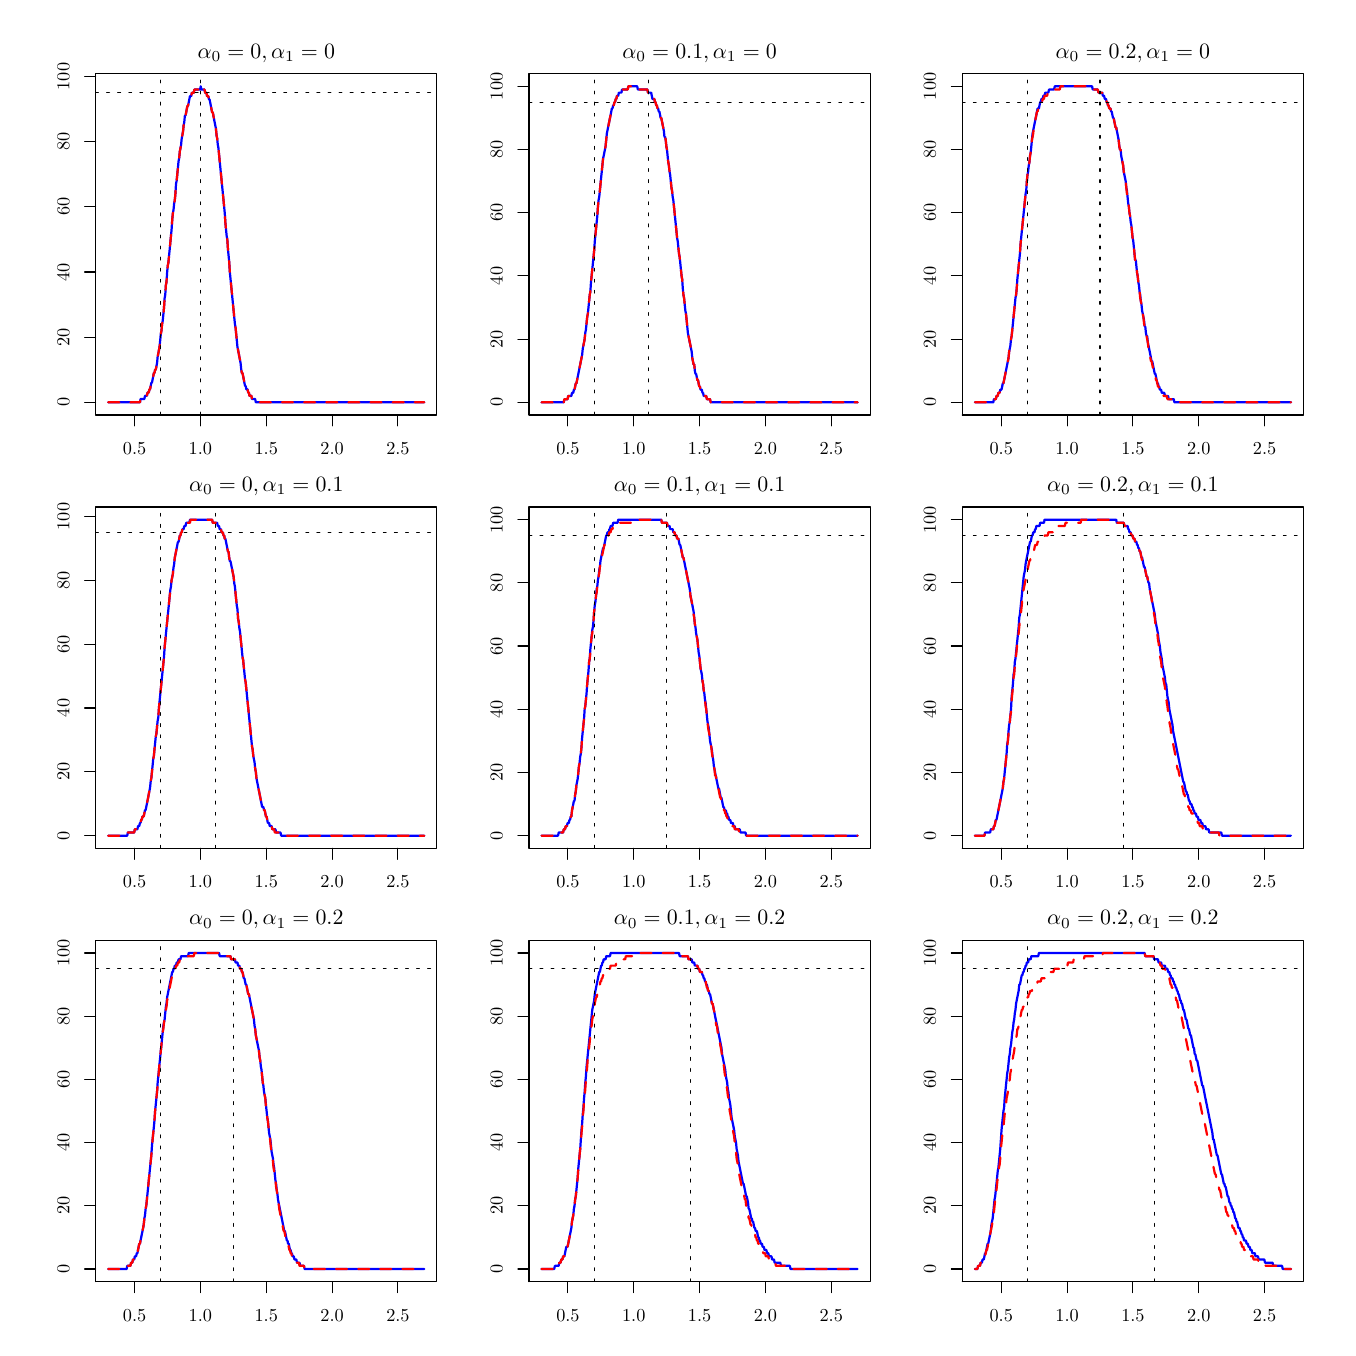
\begin{tikzpicture}[x=1pt,y=1pt]
\definecolor{fillColor}{RGB}{255,255,255}
\path[use as bounding box,fill=fillColor,fill opacity=0.00] (0,0) rectangle (469.75,469.75);
\begin{scope}
\path[clip] ( 24.55,329.80) rectangle (147.87,453.12);
\definecolor{drawColor}{RGB}{0,0,255}

\path[draw=drawColor,line width= 0.8pt,line join=round,line cap=round] ( 29.12,334.37) --
	( 29.35,334.37) --
	( 29.58,334.37) --
	( 29.81,334.37) --
	( 30.03,334.37) --
	( 30.26,334.37) --
	( 30.49,334.37) --
	( 30.72,334.37) --
	( 30.95,334.37) --
	( 31.18,334.37) --
	( 31.41,334.37) --
	( 31.64,334.37) --
	( 31.87,334.37) --
	( 32.09,334.37) --
	( 32.32,334.37) --
	( 32.55,334.37) --
	( 32.78,334.37) --
	( 33.01,334.37) --
	( 33.24,334.37) --
	( 33.47,334.37) --
	( 33.70,334.37) --
	( 33.92,334.37) --
	( 34.15,334.37) --
	( 34.38,334.37) --
	( 34.61,334.37) --
	( 34.84,334.37) --
	( 35.07,334.37) --
	( 35.30,334.37) --
	( 35.53,334.37) --
	( 35.76,334.37) --
	( 35.98,334.37) --
	( 36.21,334.37) --
	( 36.44,334.37) --
	( 36.67,334.37) --
	( 36.90,334.37) --
	( 37.13,334.37) --
	( 37.36,334.37) --
	( 37.59,334.37) --
	( 37.81,334.37) --
	( 38.04,334.37) --
	( 38.27,334.37) --
	( 38.50,334.37) --
	( 38.73,334.37) --
	( 38.96,334.37) --
	( 39.19,334.37) --
	( 39.42,334.37) --
	( 39.65,334.37) --
	( 39.87,334.37) --
	( 40.10,334.37) --
	( 40.33,334.37) --
	( 40.56,334.37) --
	( 40.79,335.55) --
	( 41.02,335.55) --
	( 41.25,335.55) --
	( 41.48,335.55) --
	( 41.71,335.55) --
	( 41.93,335.55) --
	( 42.16,335.55) --
	( 42.39,336.72) --
	( 42.62,336.72) --
	( 42.85,336.72) --
	( 43.08,336.72) --
	( 43.31,337.90) --
	( 43.54,337.90) --
	( 43.76,337.90) --
	( 43.99,339.08) --
	( 44.22,339.08) --
	( 44.45,340.26) --
	( 44.68,341.43) --
	( 44.91,341.43) --
	( 45.14,342.61) --
	( 45.37,343.79) --
	( 45.60,344.96) --
	( 45.82,344.96) --
	( 46.05,346.14) --
	( 46.28,346.14) --
	( 46.51,347.32) --
	( 46.74,348.50) --
	( 46.97,350.85) --
	( 47.20,352.03) --
	( 47.43,353.20) --
	( 47.65,354.38) --
	( 47.88,356.74) --
	( 48.11,359.09) --
	( 48.34,360.27) --
	( 48.57,362.62) --
	( 48.80,363.80) --
	( 49.03,366.15) --
	( 49.26,368.51) --
	( 49.49,372.04) --
	( 49.71,373.22) --
	( 49.94,376.75) --
	( 50.17,377.92) --
	( 50.40,381.46) --
	( 50.63,383.81) --
	( 50.86,384.99) --
	( 51.09,387.34) --
	( 51.32,389.70) --
	( 51.54,392.05) --
	( 51.77,394.41) --
	( 52.00,396.76) --
	( 52.23,400.29) --
	( 52.46,402.65) --
	( 52.69,403.82) --
	( 52.92,406.18) --
	( 53.15,407.35) --
	( 53.38,409.71) --
	( 53.60,413.24) --
	( 53.83,414.42) --
	( 54.06,416.77) --
	( 54.29,419.13) --
	( 54.52,421.48) --
	( 54.75,422.66) --
	( 54.98,425.01) --
	( 55.21,426.19) --
	( 55.43,427.37) --
	( 55.66,429.72) --
	( 55.89,430.90) --
	( 56.12,432.08) --
	( 56.35,434.43) --
	( 56.58,435.61) --
	( 56.81,437.96) --
	( 57.04,437.96) --
	( 57.27,439.14) --
	( 57.49,440.32) --
	( 57.72,441.49) --
	( 57.95,441.49) --
	( 58.18,442.67) --
	( 58.41,443.85) --
	( 58.64,445.02) --
	( 58.87,445.02) --
	( 59.10,445.02) --
	( 59.32,446.20) --
	( 59.55,446.20) --
	( 59.78,446.20) --
	( 60.01,446.20) --
	( 60.24,447.38) --
	( 60.47,447.38) --
	( 60.70,447.38) --
	( 60.93,447.38) --
	( 61.16,447.38) --
	( 61.38,447.38) --
	( 61.61,447.38) --
	( 61.84,447.38) --
	( 62.07,447.38) --
	( 62.30,447.38) --
	( 62.53,448.56) --
	( 62.76,447.38) --
	( 62.99,447.38) --
	( 63.22,447.38) --
	( 63.44,447.38) --
	( 63.67,447.38) --
	( 63.90,447.38) --
	( 64.13,446.20) --
	( 64.36,446.20) --
	( 64.59,446.20) --
	( 64.82,445.02) --
	( 65.05,445.02) --
	( 65.27,445.02) --
	( 65.50,443.85) --
	( 65.73,443.85) --
	( 65.96,442.67) --
	( 66.19,441.49) --
	( 66.42,440.32) --
	( 66.65,439.14) --
	( 66.88,439.14) --
	( 67.11,437.96) --
	( 67.33,436.78) --
	( 67.56,435.61) --
	( 67.79,434.43) --
	( 68.02,433.25) --
	( 68.25,430.90) --
	( 68.48,429.72) --
	( 68.71,427.37) --
	( 68.94,426.19) --
	( 69.16,423.83) --
	( 69.39,421.48) --
	( 69.62,419.13) --
	( 69.85,416.77) --
	( 70.08,414.42) --
	( 70.31,412.06) --
	( 70.54,409.71) --
	( 70.77,407.35) --
	( 71.00,405.00) --
	( 71.22,402.65) --
	( 71.45,399.11) --
	( 71.68,396.76) --
	( 71.91,394.41) --
	( 72.14,393.23) --
	( 72.37,389.70) --
	( 72.60,387.34) --
	( 72.83,384.99) --
	( 73.05,381.46) --
	( 73.28,379.10) --
	( 73.51,376.75) --
	( 73.74,374.39) --
	( 73.97,372.04) --
	( 74.20,369.68) --
	( 74.43,367.33) --
	( 74.66,364.98) --
	( 74.89,362.62) --
	( 75.11,361.44) --
	( 75.34,359.09) --
	( 75.57,356.74) --
	( 75.80,354.38) --
	( 76.03,353.20) --
	( 76.26,352.03) --
	( 76.49,350.85) --
	( 76.72,349.67) --
	( 76.94,348.50) --
	( 77.17,346.14) --
	( 77.40,344.96) --
	( 77.63,344.96) --
	( 77.86,343.79) --
	( 78.09,342.61) --
	( 78.32,341.43) --
	( 78.55,340.26) --
	( 78.78,340.26) --
	( 79.00,339.08) --
	( 79.23,339.08) --
	( 79.46,339.08) --
	( 79.69,337.90) --
	( 79.92,337.90) --
	( 80.15,336.72) --
	( 80.38,336.72) --
	( 80.61,336.72) --
	( 80.83,336.72) --
	( 81.06,335.55) --
	( 81.29,335.55) --
	( 81.52,335.55) --
	( 81.75,335.55) --
	( 81.98,335.55) --
	( 82.21,335.55) --
	( 82.44,334.37) --
	( 82.67,334.37) --
	( 82.89,334.37) --
	( 83.12,334.37) --
	( 83.35,334.37) --
	( 83.58,334.37) --
	( 83.81,334.37) --
	( 84.04,334.37) --
	( 84.27,334.37) --
	( 84.50,334.37) --
	( 84.73,334.37) --
	( 84.95,334.37) --
	( 85.18,334.37) --
	( 85.41,334.37) --
	( 85.64,334.37) --
	( 85.87,334.37) --
	( 86.10,334.37) --
	( 86.33,334.37) --
	( 86.56,334.37) --
	( 86.78,334.37) --
	( 87.01,334.37) --
	( 87.24,334.37) --
	( 87.47,334.37) --
	( 87.70,334.37) --
	( 87.93,334.37) --
	( 88.16,334.37) --
	( 88.39,334.37) --
	( 88.62,334.37) --
	( 88.84,334.37) --
	( 89.07,334.37) --
	( 89.30,334.37) --
	( 89.53,334.37) --
	( 89.76,334.37) --
	( 89.99,334.37) --
	( 90.22,334.37) --
	( 90.45,334.37) --
	( 90.67,334.37) --
	( 90.90,334.37) --
	( 91.13,334.37) --
	( 91.36,334.37) --
	( 91.59,334.37) --
	( 91.82,334.37) --
	( 92.05,334.37) --
	( 92.28,334.37) --
	( 92.51,334.37) --
	( 92.73,334.37) --
	( 92.96,334.37) --
	( 93.19,334.37) --
	( 93.42,334.37) --
	( 93.65,334.37) --
	( 93.88,334.37) --
	( 94.11,334.37) --
	( 94.34,334.37) --
	( 94.56,334.37) --
	( 94.79,334.37) --
	( 95.02,334.37) --
	( 95.25,334.37) --
	( 95.48,334.37) --
	( 95.71,334.37) --
	( 95.94,334.37) --
	( 96.17,334.37) --
	( 96.40,334.37) --
	( 96.62,334.37) --
	( 96.85,334.37) --
	( 97.08,334.37) --
	( 97.31,334.37) --
	( 97.54,334.37) --
	( 97.77,334.37) --
	( 98.00,334.37) --
	( 98.23,334.37) --
	( 98.45,334.37) --
	( 98.68,334.37) --
	( 98.91,334.37) --
	( 99.14,334.37) --
	( 99.37,334.37) --
	( 99.60,334.37) --
	( 99.83,334.37) --
	(100.06,334.37) --
	(100.29,334.37) --
	(100.51,334.37) --
	(100.74,334.37) --
	(100.97,334.37) --
	(101.20,334.37) --
	(101.43,334.37) --
	(101.66,334.37) --
	(101.89,334.37) --
	(102.12,334.37) --
	(102.35,334.37) --
	(102.57,334.37) --
	(102.80,334.37) --
	(103.03,334.37) --
	(103.26,334.37) --
	(103.49,334.37) --
	(103.72,334.37) --
	(103.95,334.37) --
	(104.18,334.37) --
	(104.40,334.37) --
	(104.63,334.37) --
	(104.86,334.37) --
	(105.09,334.37) --
	(105.32,334.37) --
	(105.55,334.37) --
	(105.78,334.37) --
	(106.01,334.37) --
	(106.24,334.37) --
	(106.46,334.37) --
	(106.69,334.37) --
	(106.92,334.37) --
	(107.15,334.37) --
	(107.38,334.37) --
	(107.61,334.37) --
	(107.84,334.37) --
	(108.07,334.37) --
	(108.29,334.37) --
	(108.52,334.37) --
	(108.75,334.37) --
	(108.98,334.37) --
	(109.21,334.37) --
	(109.44,334.37) --
	(109.67,334.37) --
	(109.90,334.37) --
	(110.13,334.37) --
	(110.35,334.37) --
	(110.58,334.37) --
	(110.81,334.37) --
	(111.04,334.37) --
	(111.27,334.37) --
	(111.50,334.37) --
	(111.73,334.37) --
	(111.96,334.37) --
	(112.18,334.37) --
	(112.41,334.37) --
	(112.64,334.37) --
	(112.87,334.37) --
	(113.10,334.37) --
	(113.33,334.37) --
	(113.56,334.37) --
	(113.79,334.37) --
	(114.02,334.37) --
	(114.24,334.37) --
	(114.47,334.37) --
	(114.70,334.37) --
	(114.93,334.37) --
	(115.16,334.37) --
	(115.39,334.37) --
	(115.62,334.37) --
	(115.85,334.37) --
	(116.07,334.37) --
	(116.30,334.37) --
	(116.53,334.37) --
	(116.76,334.37) --
	(116.99,334.37) --
	(117.22,334.37) --
	(117.45,334.37) --
	(117.68,334.37) --
	(117.91,334.37) --
	(118.13,334.37) --
	(118.36,334.37) --
	(118.59,334.37) --
	(118.82,334.37) --
	(119.05,334.37) --
	(119.28,334.37) --
	(119.51,334.37) --
	(119.74,334.37) --
	(119.96,334.37) --
	(120.19,334.37) --
	(120.42,334.37) --
	(120.65,334.37) --
	(120.88,334.37) --
	(121.11,334.37) --
	(121.34,334.37) --
	(121.57,334.37) --
	(121.80,334.37) --
	(122.02,334.37) --
	(122.25,334.37) --
	(122.48,334.37) --
	(122.71,334.37) --
	(122.94,334.37) --
	(123.17,334.37) --
	(123.40,334.37) --
	(123.63,334.37) --
	(123.86,334.37) --
	(124.08,334.37) --
	(124.31,334.37) --
	(124.54,334.37) --
	(124.77,334.37) --
	(125.00,334.37) --
	(125.23,334.37) --
	(125.46,334.37) --
	(125.69,334.37) --
	(125.91,334.37) --
	(126.14,334.37) --
	(126.37,334.37) --
	(126.60,334.37) --
	(126.83,334.37) --
	(127.06,334.37) --
	(127.29,334.37) --
	(127.52,334.37) --
	(127.75,334.37) --
	(127.97,334.37) --
	(128.20,334.37) --
	(128.43,334.37) --
	(128.66,334.37) --
	(128.89,334.37) --
	(129.12,334.37) --
	(129.35,334.37) --
	(129.58,334.37) --
	(129.80,334.37) --
	(130.03,334.37) --
	(130.26,334.37) --
	(130.49,334.37) --
	(130.72,334.37) --
	(130.95,334.37) --
	(131.18,334.37) --
	(131.41,334.37) --
	(131.64,334.37) --
	(131.86,334.37) --
	(132.09,334.37) --
	(132.32,334.37) --
	(132.55,334.37) --
	(132.78,334.37) --
	(133.01,334.37) --
	(133.24,334.37) --
	(133.47,334.37) --
	(133.69,334.37) --
	(133.92,334.37) --
	(134.15,334.37) --
	(134.38,334.37) --
	(134.61,334.37) --
	(134.84,334.37) --
	(135.07,334.37) --
	(135.30,334.37) --
	(135.53,334.37) --
	(135.75,334.37) --
	(135.98,334.37) --
	(136.21,334.37) --
	(136.44,334.37) --
	(136.67,334.37) --
	(136.90,334.37) --
	(137.13,334.37) --
	(137.36,334.37) --
	(137.58,334.37) --
	(137.81,334.37) --
	(138.04,334.37) --
	(138.27,334.37) --
	(138.50,334.37) --
	(138.73,334.37) --
	(138.96,334.37) --
	(139.19,334.37) --
	(139.42,334.37) --
	(139.64,334.37) --
	(139.87,334.37) --
	(140.10,334.37) --
	(140.33,334.37) --
	(140.56,334.37) --
	(140.79,334.37) --
	(141.02,334.37) --
	(141.25,334.37) --
	(141.47,334.37) --
	(141.70,334.37) --
	(141.93,334.37) --
	(142.16,334.37) --
	(142.39,334.37) --
	(142.62,334.37) --
	(142.85,334.37) --
	(143.08,334.37) --
	(143.31,334.37);
\end{scope}
\begin{scope}
\path[clip] (  0.00,  0.00) rectangle (469.75,469.75);
\definecolor{drawColor}{RGB}{0,0,0}

\path[draw=drawColor,line width= 0.4pt,line join=round,line cap=round] ( 38.63,329.80) -- (133.79,329.80);

\path[draw=drawColor,line width= 0.4pt,line join=round,line cap=round] ( 38.63,329.80) -- ( 38.63,325.84);

\path[draw=drawColor,line width= 0.4pt,line join=round,line cap=round] ( 62.42,329.80) -- ( 62.42,325.84);

\path[draw=drawColor,line width= 0.4pt,line join=round,line cap=round] ( 86.21,329.80) -- ( 86.21,325.84);

\path[draw=drawColor,line width= 0.4pt,line join=round,line cap=round] (110.00,329.80) -- (110.00,325.84);

\path[draw=drawColor,line width= 0.4pt,line join=round,line cap=round] (133.79,329.80) -- (133.79,325.84);

\node[text=drawColor,anchor=base,inner sep=0pt, outer sep=0pt, scale=  0.66] at ( 38.63,315.55) {0.5};

\node[text=drawColor,anchor=base,inner sep=0pt, outer sep=0pt, scale=  0.66] at ( 62.42,315.55) {1.0};

\node[text=drawColor,anchor=base,inner sep=0pt, outer sep=0pt, scale=  0.66] at ( 86.21,315.55) {1.5};

\node[text=drawColor,anchor=base,inner sep=0pt, outer sep=0pt, scale=  0.66] at (110.00,315.55) {2.0};

\node[text=drawColor,anchor=base,inner sep=0pt, outer sep=0pt, scale=  0.66] at (133.79,315.55) {2.5};

\path[draw=drawColor,line width= 0.4pt,line join=round,line cap=round] ( 24.55,334.37) -- ( 24.55,452.09);

\path[draw=drawColor,line width= 0.4pt,line join=round,line cap=round] ( 24.55,334.37) -- ( 20.59,334.37);

\path[draw=drawColor,line width= 0.4pt,line join=round,line cap=round] ( 24.55,357.91) -- ( 20.59,357.91);

\path[draw=drawColor,line width= 0.4pt,line join=round,line cap=round] ( 24.55,381.46) -- ( 20.59,381.46);

\path[draw=drawColor,line width= 0.4pt,line join=round,line cap=round] ( 24.55,405.00) -- ( 20.59,405.00);

\path[draw=drawColor,line width= 0.4pt,line join=round,line cap=round] ( 24.55,428.54) -- ( 20.59,428.54);

\path[draw=drawColor,line width= 0.4pt,line join=round,line cap=round] ( 24.55,452.09) -- ( 20.59,452.09);

\node[text=drawColor,rotate= 90.00,anchor=base,inner sep=0pt, outer sep=0pt, scale=  0.66] at ( 15.05,334.37) {0};

\node[text=drawColor,rotate= 90.00,anchor=base,inner sep=0pt, outer sep=0pt, scale=  0.66] at ( 15.05,357.91) {20};

\node[text=drawColor,rotate= 90.00,anchor=base,inner sep=0pt, outer sep=0pt, scale=  0.66] at ( 15.05,381.46) {40};

\node[text=drawColor,rotate= 90.00,anchor=base,inner sep=0pt, outer sep=0pt, scale=  0.66] at ( 15.05,405.00) {60};

\node[text=drawColor,rotate= 90.00,anchor=base,inner sep=0pt, outer sep=0pt, scale=  0.66] at ( 15.05,428.54) {80};

\node[text=drawColor,rotate= 90.00,anchor=base,inner sep=0pt, outer sep=0pt, scale=  0.66] at ( 15.05,452.09) {100};

\path[draw=drawColor,line width= 0.4pt,line join=round,line cap=round] ( 24.55,329.80) --
	(147.87,329.80) --
	(147.87,453.12) --
	( 24.55,453.12) --
	( 24.55,329.80);
\end{scope}
\begin{scope}
\path[clip] (  0.00,313.17) rectangle (156.58,469.75);
\definecolor{drawColor}{RGB}{0,0,0}

\node[text=drawColor,anchor=base,inner sep=0pt, outer sep=0pt, scale=  0.79] at ( 86.21,458.71) {\bfseries $\alpha_0 = 0, \alpha_1 = 0$};
\end{scope}
\begin{scope}
\path[clip] ( 24.55,329.80) rectangle (147.87,453.12);
\definecolor{drawColor}{RGB}{255,0,0}

\path[draw=drawColor,line width= 0.8pt,dash pattern=on 4pt off 4pt ,line join=round,line cap=round] ( 29.12,334.37) --
	( 29.35,334.37) --
	( 29.58,334.37) --
	( 29.81,334.37) --
	( 30.03,334.37) --
	( 30.26,334.37) --
	( 30.49,334.37) --
	( 30.72,334.37) --
	( 30.95,334.37) --
	( 31.18,334.37) --
	( 31.41,334.37) --
	( 31.64,334.37) --
	( 31.87,334.37) --
	( 32.09,334.37) --
	( 32.32,334.37) --
	( 32.55,334.37) --
	( 32.78,334.37) --
	( 33.01,334.37) --
	( 33.24,334.37) --
	( 33.47,334.37) --
	( 33.70,334.37) --
	( 33.92,334.37) --
	( 34.15,334.37) --
	( 34.38,334.37) --
	( 34.61,334.37) --
	( 34.84,334.37) --
	( 35.07,334.37) --
	( 35.30,334.37) --
	( 35.53,334.37) --
	( 35.76,334.37) --
	( 35.98,334.37) --
	( 36.21,334.37) --
	( 36.44,334.37) --
	( 36.67,334.37) --
	( 36.90,334.37) --
	( 37.13,334.37) --
	( 37.36,334.37) --
	( 37.59,334.37) --
	( 37.81,334.37) --
	( 38.04,334.37) --
	( 38.27,334.37) --
	( 38.50,334.37) --
	( 38.73,334.37) --
	( 38.96,334.37) --
	( 39.19,334.37) --
	( 39.42,334.37) --
	( 39.65,334.37) --
	( 39.87,334.37) --
	( 40.10,334.37) --
	( 40.33,334.37) --
	( 40.56,334.37) --
	( 40.79,335.55) --
	( 41.02,335.55) --
	( 41.25,335.55) --
	( 41.48,335.55) --
	( 41.71,335.55) --
	( 41.93,335.55) --
	( 42.16,335.55) --
	( 42.39,336.72) --
	( 42.62,336.72) --
	( 42.85,336.72) --
	( 43.08,336.72) --
	( 43.31,337.90) --
	( 43.54,337.90) --
	( 43.76,337.90) --
	( 43.99,339.08) --
	( 44.22,339.08) --
	( 44.45,340.26) --
	( 44.68,341.43) --
	( 44.91,341.43) --
	( 45.14,342.61) --
	( 45.37,343.79) --
	( 45.60,344.96) --
	( 45.82,344.96) --
	( 46.05,346.14) --
	( 46.28,346.14) --
	( 46.51,347.32) --
	( 46.74,348.50) --
	( 46.97,350.85) --
	( 47.20,352.03) --
	( 47.43,353.20) --
	( 47.65,354.38) --
	( 47.88,356.74) --
	( 48.11,359.09) --
	( 48.34,360.27) --
	( 48.57,362.62) --
	( 48.80,363.80) --
	( 49.03,366.15) --
	( 49.26,368.51) --
	( 49.49,372.04) --
	( 49.71,373.22) --
	( 49.94,376.75) --
	( 50.17,377.92) --
	( 50.40,381.46) --
	( 50.63,383.81) --
	( 50.86,384.99) --
	( 51.09,387.34) --
	( 51.32,389.70) --
	( 51.54,392.05) --
	( 51.77,394.41) --
	( 52.00,396.76) --
	( 52.23,400.29) --
	( 52.46,402.65) --
	( 52.69,403.82) --
	( 52.92,406.18) --
	( 53.15,407.35) --
	( 53.38,409.71) --
	( 53.60,413.24) --
	( 53.83,414.42) --
	( 54.06,416.77) --
	( 54.29,419.13) --
	( 54.52,421.48) --
	( 54.75,422.66) --
	( 54.98,425.01) --
	( 55.21,426.19) --
	( 55.43,427.37) --
	( 55.66,429.72) --
	( 55.89,430.90) --
	( 56.12,432.08) --
	( 56.35,434.43) --
	( 56.58,435.61) --
	( 56.81,437.96) --
	( 57.04,437.96) --
	( 57.27,439.14) --
	( 57.49,440.32) --
	( 57.72,441.49) --
	( 57.95,441.49) --
	( 58.18,442.67) --
	( 58.41,443.85) --
	( 58.64,445.02) --
	( 58.87,445.02) --
	( 59.10,445.02) --
	( 59.32,446.20) --
	( 59.55,446.20) --
	( 59.78,446.20) --
	( 60.01,446.20) --
	( 60.24,447.38) --
	( 60.47,447.38) --
	( 60.70,447.38) --
	( 60.93,447.38) --
	( 61.16,447.38) --
	( 61.38,447.38) --
	( 61.61,447.38) --
	( 61.84,447.38) --
	( 62.07,447.38) --
	( 62.30,447.38) --
	( 62.53,448.56) --
	( 62.76,447.38) --
	( 62.99,447.38) --
	( 63.22,447.38) --
	( 63.44,447.38) --
	( 63.67,447.38) --
	( 63.90,447.38) --
	( 64.13,446.20) --
	( 64.36,446.20) --
	( 64.59,446.20) --
	( 64.82,445.02) --
	( 65.05,445.02) --
	( 65.27,445.02) --
	( 65.50,443.85) --
	( 65.73,443.85) --
	( 65.96,442.67) --
	( 66.19,441.49) --
	( 66.42,440.32) --
	( 66.65,439.14) --
	( 66.88,439.14) --
	( 67.11,437.96) --
	( 67.33,436.78) --
	( 67.56,435.61) --
	( 67.79,434.43) --
	( 68.02,433.25) --
	( 68.25,430.90) --
	( 68.48,429.72) --
	( 68.71,427.37) --
	( 68.94,426.19) --
	( 69.16,423.83) --
	( 69.39,421.48) --
	( 69.62,419.13) --
	( 69.85,416.77) --
	( 70.08,414.42) --
	( 70.31,412.06) --
	( 70.54,409.71) --
	( 70.77,407.35) --
	( 71.00,405.00) --
	( 71.22,402.65) --
	( 71.45,399.11) --
	( 71.68,396.76) --
	( 71.91,394.41) --
	( 72.14,393.23) --
	( 72.37,389.70) --
	( 72.60,387.34) --
	( 72.83,384.99) --
	( 73.05,381.46) --
	( 73.28,379.10) --
	( 73.51,376.75) --
	( 73.74,374.39) --
	( 73.97,372.04) --
	( 74.20,369.68) --
	( 74.43,367.33) --
	( 74.66,364.98) --
	( 74.89,362.62) --
	( 75.11,361.44) --
	( 75.34,359.09) --
	( 75.57,356.74) --
	( 75.80,354.38) --
	( 76.03,353.20) --
	( 76.26,352.03) --
	( 76.49,350.85) --
	( 76.72,349.67) --
	( 76.94,348.50) --
	( 77.17,346.14) --
	( 77.40,344.96) --
	( 77.63,344.96) --
	( 77.86,343.79) --
	( 78.09,342.61) --
	( 78.32,341.43) --
	( 78.55,340.26) --
	( 78.78,340.26) --
	( 79.00,339.08) --
	( 79.23,339.08) --
	( 79.46,339.08) --
	( 79.69,337.90) --
	( 79.92,337.90) --
	( 80.15,336.72) --
	( 80.38,336.72) --
	( 80.61,336.72) --
	( 80.83,336.72) --
	( 81.06,335.55) --
	( 81.29,335.55) --
	( 81.52,335.55) --
	( 81.75,335.55) --
	( 81.98,335.55) --
	( 82.21,335.55) --
	( 82.44,334.37) --
	( 82.67,334.37) --
	( 82.89,334.37) --
	( 83.12,334.37) --
	( 83.35,334.37) --
	( 83.58,334.37) --
	( 83.81,334.37) --
	( 84.04,334.37) --
	( 84.27,334.37) --
	( 84.50,334.37) --
	( 84.73,334.37) --
	( 84.95,334.37) --
	( 85.18,334.37) --
	( 85.41,334.37) --
	( 85.64,334.37) --
	( 85.87,334.37) --
	( 86.10,334.37) --
	( 86.33,334.37) --
	( 86.56,334.37) --
	( 86.78,334.37) --
	( 87.01,334.37) --
	( 87.24,334.37) --
	( 87.47,334.37) --
	( 87.70,334.37) --
	( 87.93,334.37) --
	( 88.16,334.37) --
	( 88.39,334.37) --
	( 88.62,334.37) --
	( 88.84,334.37) --
	( 89.07,334.37) --
	( 89.30,334.37) --
	( 89.53,334.37) --
	( 89.76,334.37) --
	( 89.99,334.37) --
	( 90.22,334.37) --
	( 90.45,334.37) --
	( 90.67,334.37) --
	( 90.90,334.37) --
	( 91.13,334.37) --
	( 91.36,334.37) --
	( 91.59,334.37) --
	( 91.82,334.37) --
	( 92.05,334.37) --
	( 92.28,334.37) --
	( 92.51,334.37) --
	( 92.73,334.37) --
	( 92.96,334.37) --
	( 93.19,334.37) --
	( 93.42,334.37) --
	( 93.65,334.37) --
	( 93.88,334.37) --
	( 94.11,334.37) --
	( 94.34,334.37) --
	( 94.56,334.37) --
	( 94.79,334.37) --
	( 95.02,334.37) --
	( 95.25,334.37) --
	( 95.48,334.37) --
	( 95.71,334.37) --
	( 95.94,334.37) --
	( 96.17,334.37) --
	( 96.40,334.37) --
	( 96.62,334.37) --
	( 96.85,334.37) --
	( 97.08,334.37) --
	( 97.31,334.37) --
	( 97.54,334.37) --
	( 97.77,334.37) --
	( 98.00,334.37) --
	( 98.23,334.37) --
	( 98.45,334.37) --
	( 98.68,334.37) --
	( 98.91,334.37) --
	( 99.14,334.37) --
	( 99.37,334.37) --
	( 99.60,334.37) --
	( 99.83,334.37) --
	(100.06,334.37) --
	(100.29,334.37) --
	(100.51,334.37) --
	(100.74,334.37) --
	(100.97,334.37) --
	(101.20,334.37) --
	(101.43,334.37) --
	(101.66,334.37) --
	(101.89,334.37) --
	(102.12,334.37) --
	(102.35,334.37) --
	(102.57,334.37) --
	(102.80,334.37) --
	(103.03,334.37) --
	(103.26,334.37) --
	(103.49,334.37) --
	(103.72,334.37) --
	(103.95,334.37) --
	(104.18,334.37) --
	(104.40,334.37) --
	(104.63,334.37) --
	(104.86,334.37) --
	(105.09,334.37) --
	(105.32,334.37) --
	(105.55,334.37) --
	(105.78,334.37) --
	(106.01,334.37) --
	(106.24,334.37) --
	(106.46,334.37) --
	(106.69,334.37) --
	(106.92,334.37) --
	(107.15,334.37) --
	(107.38,334.37) --
	(107.61,334.37) --
	(107.84,334.37) --
	(108.07,334.37) --
	(108.29,334.37) --
	(108.52,334.37) --
	(108.75,334.37) --
	(108.98,334.37) --
	(109.21,334.37) --
	(109.44,334.37) --
	(109.67,334.37) --
	(109.90,334.37) --
	(110.13,334.37) --
	(110.35,334.37) --
	(110.58,334.37) --
	(110.81,334.37) --
	(111.04,334.37) --
	(111.27,334.37) --
	(111.50,334.37) --
	(111.73,334.37) --
	(111.96,334.37) --
	(112.18,334.37) --
	(112.41,334.37) --
	(112.64,334.37) --
	(112.87,334.37) --
	(113.10,334.37) --
	(113.33,334.37) --
	(113.56,334.37) --
	(113.79,334.37) --
	(114.02,334.37) --
	(114.24,334.37) --
	(114.47,334.37) --
	(114.70,334.37) --
	(114.93,334.37) --
	(115.16,334.37) --
	(115.39,334.37) --
	(115.62,334.37) --
	(115.85,334.37) --
	(116.07,334.37) --
	(116.30,334.37) --
	(116.53,334.37) --
	(116.76,334.37) --
	(116.99,334.37) --
	(117.22,334.37) --
	(117.45,334.37) --
	(117.68,334.37) --
	(117.91,334.37) --
	(118.13,334.37) --
	(118.36,334.37) --
	(118.59,334.37) --
	(118.82,334.37) --
	(119.05,334.37) --
	(119.28,334.37) --
	(119.51,334.37) --
	(119.74,334.37) --
	(119.96,334.37) --
	(120.19,334.37) --
	(120.42,334.37) --
	(120.65,334.37) --
	(120.88,334.37) --
	(121.11,334.37) --
	(121.34,334.37) --
	(121.57,334.37) --
	(121.80,334.37) --
	(122.02,334.37) --
	(122.25,334.37) --
	(122.48,334.37) --
	(122.71,334.37) --
	(122.94,334.37) --
	(123.17,334.37) --
	(123.40,334.37) --
	(123.63,334.37) --
	(123.86,334.37) --
	(124.08,334.37) --
	(124.31,334.37) --
	(124.54,334.37) --
	(124.77,334.37) --
	(125.00,334.37) --
	(125.23,334.37) --
	(125.46,334.37) --
	(125.69,334.37) --
	(125.91,334.37) --
	(126.14,334.37) --
	(126.37,334.37) --
	(126.60,334.37) --
	(126.83,334.37) --
	(127.06,334.37) --
	(127.29,334.37) --
	(127.52,334.37) --
	(127.75,334.37) --
	(127.97,334.37) --
	(128.20,334.37) --
	(128.43,334.37) --
	(128.66,334.37) --
	(128.89,334.37) --
	(129.12,334.37) --
	(129.35,334.37) --
	(129.58,334.37) --
	(129.80,334.37) --
	(130.03,334.37) --
	(130.26,334.37) --
	(130.49,334.37) --
	(130.72,334.37) --
	(130.95,334.37) --
	(131.18,334.37) --
	(131.41,334.37) --
	(131.64,334.37) --
	(131.86,334.37) --
	(132.09,334.37) --
	(132.32,334.37) --
	(132.55,334.37) --
	(132.78,334.37) --
	(133.01,334.37) --
	(133.24,334.37) --
	(133.47,334.37) --
	(133.69,334.37) --
	(133.92,334.37) --
	(134.15,334.37) --
	(134.38,334.37) --
	(134.61,334.37) --
	(134.84,334.37) --
	(135.07,334.37) --
	(135.30,334.37) --
	(135.53,334.37) --
	(135.75,334.37) --
	(135.98,334.37) --
	(136.21,334.37) --
	(136.44,334.37) --
	(136.67,334.37) --
	(136.90,334.37) --
	(137.13,334.37) --
	(137.36,334.37) --
	(137.58,334.37) --
	(137.81,334.37) --
	(138.04,334.37) --
	(138.27,334.37) --
	(138.50,334.37) --
	(138.73,334.37) --
	(138.96,334.37) --
	(139.19,334.37) --
	(139.42,334.37) --
	(139.64,334.37) --
	(139.87,334.37) --
	(140.10,334.37) --
	(140.33,334.37) --
	(140.56,334.37) --
	(140.79,334.37) --
	(141.02,334.37) --
	(141.25,334.37) --
	(141.47,334.37) --
	(141.70,334.37) --
	(141.93,334.37) --
	(142.16,334.37) --
	(142.39,334.37) --
	(142.62,334.37) --
	(142.85,334.37) --
	(143.08,334.37) --
	(143.31,334.37);
\definecolor{drawColor}{RGB}{0,0,0}

\path[draw=drawColor,line width= 0.4pt,dash pattern=on 1pt off 3pt ,line join=round,line cap=round] ( 24.55,446.20) -- (147.87,446.20);

\path[draw=drawColor,line width= 0.4pt,dash pattern=on 1pt off 3pt ,line join=round,line cap=round] ( 48.15,329.80) -- ( 48.15,453.12);

\path[draw=drawColor,line width= 0.4pt,dash pattern=on 1pt off 3pt ,line join=round,line cap=round] ( 62.42,329.80) -- ( 62.42,453.12);
\end{scope}
\begin{scope}
\path[clip] (181.14,329.80) rectangle (304.46,453.12);
\definecolor{drawColor}{RGB}{0,0,255}

\path[draw=drawColor,line width= 0.8pt,line join=round,line cap=round] (185.70,334.37) --
	(185.93,334.37) --
	(186.16,334.37) --
	(186.39,334.37) --
	(186.62,334.37) --
	(186.85,334.37) --
	(187.08,334.37) --
	(187.31,334.37) --
	(187.54,334.37) --
	(187.76,334.37) --
	(187.99,334.37) --
	(188.22,334.37) --
	(188.45,334.37) --
	(188.68,334.37) --
	(188.91,334.37) --
	(189.14,334.37) --
	(189.37,334.37) --
	(189.59,334.37) --
	(189.82,334.37) --
	(190.05,334.37) --
	(190.28,334.37) --
	(190.51,334.37) --
	(190.74,334.37) --
	(190.97,334.37) --
	(191.20,334.37) --
	(191.43,334.37) --
	(191.65,334.37) --
	(191.88,334.37) --
	(192.11,334.37) --
	(192.34,334.37) --
	(192.57,334.37) --
	(192.80,334.37) --
	(193.03,334.37) --
	(193.26,334.37) --
	(193.48,334.37) --
	(193.71,334.37) --
	(193.94,335.51) --
	(194.17,335.51) --
	(194.40,335.51) --
	(194.63,335.51) --
	(194.86,335.51) --
	(195.09,335.51) --
	(195.32,336.65) --
	(195.54,336.65) --
	(195.77,336.65) --
	(196.00,336.65) --
	(196.23,336.65) --
	(196.46,336.65) --
	(196.69,337.80) --
	(196.92,337.80) --
	(197.15,337.80) --
	(197.37,338.94) --
	(197.60,338.94) --
	(197.83,340.08) --
	(198.06,341.22) --
	(198.29,341.22) --
	(198.52,342.36) --
	(198.75,343.50) --
	(198.98,344.65) --
	(199.21,345.79) --
	(199.43,346.93) --
	(199.66,348.07) --
	(199.89,349.21) --
	(200.12,350.36) --
	(200.35,351.50) --
	(200.58,353.78) --
	(200.81,354.92) --
	(201.04,356.06) --
	(201.26,357.21) --
	(201.49,359.49) --
	(201.72,360.63) --
	(201.95,362.92) --
	(202.18,365.20) --
	(202.41,366.34) --
	(202.64,368.63) --
	(202.87,370.91) --
	(203.10,373.19) --
	(203.32,374.33) --
	(203.55,377.76) --
	(203.78,380.04) --
	(204.01,382.33) --
	(204.24,384.61) --
	(204.47,386.90) --
	(204.70,389.18) --
	(204.93,392.60) --
	(205.15,394.89) --
	(205.38,397.17) --
	(205.61,399.46) --
	(205.84,401.74) --
	(206.07,405.16) --
	(206.30,407.45) --
	(206.53,408.59) --
	(206.76,410.87) --
	(206.99,413.16) --
	(207.21,415.44) --
	(207.44,417.73) --
	(207.67,420.01) --
	(207.90,422.29) --
	(208.13,423.43) --
	(208.36,424.58) --
	(208.59,425.72) --
	(208.82,426.86) --
	(209.05,429.14) --
	(209.27,431.43) --
	(209.50,432.57) --
	(209.73,433.71) --
	(209.96,434.85) --
	(210.19,436.00) --
	(210.42,437.14) --
	(210.65,438.28) --
	(210.88,439.42) --
	(211.10,440.56) --
	(211.33,440.56) --
	(211.56,441.70) --
	(211.79,441.70) --
	(212.02,442.85) --
	(212.25,442.85) --
	(212.48,443.99) --
	(212.71,443.99) --
	(212.94,445.13) --
	(213.16,445.13) --
	(213.39,445.13) --
	(213.62,446.27) --
	(213.85,446.27) --
	(214.08,446.27) --
	(214.31,446.27) --
	(214.54,446.27) --
	(214.77,447.41) --
	(214.99,447.41) --
	(215.22,447.41) --
	(215.45,447.41) --
	(215.68,447.41) --
	(215.91,447.41) --
	(216.14,447.41) --
	(216.37,447.41) --
	(216.60,447.41) --
	(216.83,447.41) --
	(217.05,448.56) --
	(217.28,448.56) --
	(217.51,448.56) --
	(217.74,448.56) --
	(217.97,448.56) --
	(218.20,448.56) --
	(218.43,448.56) --
	(218.66,448.56) --
	(218.88,448.56) --
	(219.11,448.56) --
	(219.34,448.56) --
	(219.57,448.56) --
	(219.80,448.56) --
	(220.03,448.56) --
	(220.26,448.56) --
	(220.49,447.41) --
	(220.72,447.41) --
	(220.94,447.41) --
	(221.17,447.41) --
	(221.40,447.41) --
	(221.63,447.41) --
	(221.86,447.41) --
	(222.09,447.41) --
	(222.32,447.41) --
	(222.55,447.41) --
	(222.77,447.41) --
	(223.00,447.41) --
	(223.23,447.41) --
	(223.46,447.41) --
	(223.69,447.41) --
	(223.92,447.41) --
	(224.15,446.27) --
	(224.38,446.27) --
	(224.61,446.27) --
	(224.83,446.27) --
	(225.06,446.27) --
	(225.29,446.27) --
	(225.52,445.13) --
	(225.75,443.99) --
	(225.98,443.99) --
	(226.21,443.99) --
	(226.44,443.99) --
	(226.66,442.85) --
	(226.89,442.85) --
	(227.12,441.70) --
	(227.35,441.70) --
	(227.58,440.56) --
	(227.81,440.56) --
	(228.04,439.42) --
	(228.27,439.42) --
	(228.50,438.28) --
	(228.72,437.14) --
	(228.95,437.14) --
	(229.18,436.00) --
	(229.41,434.85) --
	(229.64,433.71) --
	(229.87,432.57) --
	(230.10,430.29) --
	(230.33,430.29) --
	(230.56,429.14) --
	(230.78,426.86) --
	(231.01,425.72) --
	(231.24,423.43) --
	(231.47,421.15) --
	(231.70,420.01) --
	(231.93,417.73) --
	(232.16,416.58) --
	(232.39,414.30) --
	(232.61,412.02) --
	(232.84,410.87) --
	(233.07,408.59) --
	(233.30,407.45) --
	(233.53,405.16) --
	(233.76,402.88) --
	(233.99,400.60) --
	(234.22,398.31) --
	(234.45,396.03) --
	(234.67,393.75) --
	(234.90,392.60) --
	(235.13,390.32) --
	(235.36,388.04) --
	(235.59,386.90) --
	(235.82,384.61) --
	(236.05,382.33) --
	(236.28,380.04) --
	(236.50,378.90) --
	(236.73,375.48) --
	(236.96,373.19) --
	(237.19,372.05) --
	(237.42,369.77) --
	(237.65,367.48) --
	(237.88,366.34) --
	(238.11,364.06) --
	(238.34,361.77) --
	(238.56,359.49) --
	(238.79,358.35) --
	(239.02,357.21) --
	(239.25,356.06) --
	(239.48,354.92) --
	(239.71,353.78) --
	(239.94,352.64) --
	(240.17,350.36) --
	(240.39,349.21) --
	(240.62,348.07) --
	(240.85,348.07) --
	(241.08,345.79) --
	(241.31,344.65) --
	(241.54,344.65) --
	(241.77,343.50) --
	(242.00,342.36) --
	(242.23,342.36) --
	(242.45,341.22) --
	(242.68,340.08) --
	(242.91,340.08) --
	(243.14,338.94) --
	(243.37,338.94) --
	(243.60,338.94) --
	(243.83,337.80) --
	(244.06,337.80) --
	(244.28,336.65) --
	(244.51,336.65) --
	(244.74,336.65) --
	(244.97,336.65) --
	(245.20,336.65) --
	(245.43,335.51) --
	(245.66,335.51) --
	(245.89,335.51) --
	(246.12,335.51) --
	(246.34,335.51) --
	(246.57,335.51) --
	(246.80,334.37) --
	(247.03,334.37) --
	(247.26,334.37) --
	(247.49,334.37) --
	(247.72,334.37) --
	(247.95,334.37) --
	(248.18,334.37) --
	(248.40,334.37) --
	(248.63,334.37) --
	(248.86,334.37) --
	(249.09,334.37) --
	(249.32,334.37) --
	(249.55,334.37) --
	(249.78,334.37) --
	(250.01,334.37) --
	(250.23,334.37) --
	(250.46,334.37) --
	(250.69,334.37) --
	(250.92,334.37) --
	(251.15,334.37) --
	(251.38,334.37) --
	(251.61,334.37) --
	(251.84,334.37) --
	(252.07,334.37) --
	(252.29,334.37) --
	(252.52,334.37) --
	(252.75,334.37) --
	(252.98,334.37) --
	(253.21,334.37) --
	(253.44,334.37) --
	(253.67,334.37) --
	(253.90,334.37) --
	(254.12,334.37) --
	(254.35,334.37) --
	(254.58,334.37) --
	(254.81,334.37) --
	(255.04,334.37) --
	(255.27,334.37) --
	(255.50,334.37) --
	(255.73,334.37) --
	(255.96,334.37) --
	(256.18,334.37) --
	(256.41,334.37) --
	(256.64,334.37) --
	(256.87,334.37) --
	(257.10,334.37) --
	(257.33,334.37) --
	(257.56,334.37) --
	(257.79,334.37) --
	(258.01,334.37) --
	(258.24,334.37) --
	(258.47,334.37) --
	(258.70,334.37) --
	(258.93,334.37) --
	(259.16,334.37) --
	(259.39,334.37) --
	(259.62,334.37) --
	(259.85,334.37) --
	(260.07,334.37) --
	(260.30,334.37) --
	(260.53,334.37) --
	(260.76,334.37) --
	(260.99,334.37) --
	(261.22,334.37) --
	(261.45,334.37) --
	(261.68,334.37) --
	(261.90,334.37) --
	(262.13,334.37) --
	(262.36,334.37) --
	(262.59,334.37) --
	(262.82,334.37) --
	(263.05,334.37) --
	(263.28,334.37) --
	(263.51,334.37) --
	(263.74,334.37) --
	(263.96,334.37) --
	(264.19,334.37) --
	(264.42,334.37) --
	(264.65,334.37) --
	(264.88,334.37) --
	(265.11,334.37) --
	(265.34,334.37) --
	(265.57,334.37) --
	(265.79,334.37) --
	(266.02,334.37) --
	(266.25,334.37) --
	(266.48,334.37) --
	(266.71,334.37) --
	(266.94,334.37) --
	(267.17,334.37) --
	(267.40,334.37) --
	(267.63,334.37) --
	(267.85,334.37) --
	(268.08,334.37) --
	(268.31,334.37) --
	(268.54,334.37) --
	(268.77,334.37) --
	(269.00,334.37) --
	(269.23,334.37) --
	(269.46,334.37) --
	(269.69,334.37) --
	(269.91,334.37) --
	(270.14,334.37) --
	(270.37,334.37) --
	(270.60,334.37) --
	(270.83,334.37) --
	(271.06,334.37) --
	(271.29,334.37) --
	(271.52,334.37) --
	(271.74,334.37) --
	(271.97,334.37) --
	(272.20,334.37) --
	(272.43,334.37) --
	(272.66,334.37) --
	(272.89,334.37) --
	(273.12,334.37) --
	(273.35,334.37) --
	(273.58,334.37) --
	(273.80,334.37) --
	(274.03,334.37) --
	(274.26,334.37) --
	(274.49,334.37) --
	(274.72,334.37) --
	(274.95,334.37) --
	(275.18,334.37) --
	(275.41,334.37) --
	(275.63,334.37) --
	(275.86,334.37) --
	(276.09,334.37) --
	(276.32,334.37) --
	(276.55,334.37) --
	(276.78,334.37) --
	(277.01,334.37) --
	(277.24,334.37) --
	(277.47,334.37) --
	(277.69,334.37) --
	(277.92,334.37) --
	(278.15,334.37) --
	(278.38,334.37) --
	(278.61,334.37) --
	(278.84,334.37) --
	(279.07,334.37) --
	(279.30,334.37) --
	(279.52,334.37) --
	(279.75,334.37) --
	(279.98,334.37) --
	(280.21,334.37) --
	(280.44,334.37) --
	(280.67,334.37) --
	(280.90,334.37) --
	(281.13,334.37) --
	(281.36,334.37) --
	(281.58,334.37) --
	(281.81,334.37) --
	(282.04,334.37) --
	(282.27,334.37) --
	(282.50,334.37) --
	(282.73,334.37) --
	(282.96,334.37) --
	(283.19,334.37) --
	(283.41,334.37) --
	(283.64,334.37) --
	(283.87,334.37) --
	(284.10,334.37) --
	(284.33,334.37) --
	(284.56,334.37) --
	(284.79,334.37) --
	(285.02,334.37) --
	(285.25,334.37) --
	(285.47,334.37) --
	(285.70,334.37) --
	(285.93,334.37) --
	(286.16,334.37) --
	(286.39,334.37) --
	(286.62,334.37) --
	(286.85,334.37) --
	(287.08,334.37) --
	(287.30,334.37) --
	(287.53,334.37) --
	(287.76,334.37) --
	(287.99,334.37) --
	(288.22,334.37) --
	(288.45,334.37) --
	(288.68,334.37) --
	(288.91,334.37) --
	(289.14,334.37) --
	(289.36,334.37) --
	(289.59,334.37) --
	(289.82,334.37) --
	(290.05,334.37) --
	(290.28,334.37) --
	(290.51,334.37) --
	(290.74,334.37) --
	(290.97,334.37) --
	(291.20,334.37) --
	(291.42,334.37) --
	(291.65,334.37) --
	(291.88,334.37) --
	(292.11,334.37) --
	(292.34,334.37) --
	(292.57,334.37) --
	(292.80,334.37) --
	(293.03,334.37) --
	(293.25,334.37) --
	(293.48,334.37) --
	(293.71,334.37) --
	(293.94,334.37) --
	(294.17,334.37) --
	(294.40,334.37) --
	(294.63,334.37) --
	(294.86,334.37) --
	(295.09,334.37) --
	(295.31,334.37) --
	(295.54,334.37) --
	(295.77,334.37) --
	(296.00,334.37) --
	(296.23,334.37) --
	(296.46,334.37) --
	(296.69,334.37) --
	(296.92,334.37) --
	(297.14,334.37) --
	(297.37,334.37) --
	(297.60,334.37) --
	(297.83,334.37) --
	(298.06,334.37) --
	(298.29,334.37) --
	(298.52,334.37) --
	(298.75,334.37) --
	(298.98,334.37) --
	(299.20,334.37) --
	(299.43,334.37) --
	(299.66,334.37) --
	(299.89,334.37);
\end{scope}
\begin{scope}
\path[clip] (  0.00,  0.00) rectangle (469.75,469.75);
\definecolor{drawColor}{RGB}{0,0,0}

\path[draw=drawColor,line width= 0.4pt,line join=round,line cap=round] (195.22,329.80) -- (290.38,329.80);

\path[draw=drawColor,line width= 0.4pt,line join=round,line cap=round] (195.22,329.80) -- (195.22,325.84);

\path[draw=drawColor,line width= 0.4pt,line join=round,line cap=round] (219.01,329.80) -- (219.01,325.84);

\path[draw=drawColor,line width= 0.4pt,line join=round,line cap=round] (242.80,329.80) -- (242.80,325.84);

\path[draw=drawColor,line width= 0.4pt,line join=round,line cap=round] (266.59,329.80) -- (266.59,325.84);

\path[draw=drawColor,line width= 0.4pt,line join=round,line cap=round] (290.38,329.80) -- (290.38,325.84);

\node[text=drawColor,anchor=base,inner sep=0pt, outer sep=0pt, scale=  0.66] at (195.22,315.55) {0.5};

\node[text=drawColor,anchor=base,inner sep=0pt, outer sep=0pt, scale=  0.66] at (219.01,315.55) {1.0};

\node[text=drawColor,anchor=base,inner sep=0pt, outer sep=0pt, scale=  0.66] at (242.80,315.55) {1.5};

\node[text=drawColor,anchor=base,inner sep=0pt, outer sep=0pt, scale=  0.66] at (266.59,315.55) {2.0};

\node[text=drawColor,anchor=base,inner sep=0pt, outer sep=0pt, scale=  0.66] at (290.38,315.55) {2.5};

\path[draw=drawColor,line width= 0.4pt,line join=round,line cap=round] (181.14,334.37) -- (181.14,448.56);

\path[draw=drawColor,line width= 0.4pt,line join=round,line cap=round] (181.14,334.37) -- (177.18,334.37);

\path[draw=drawColor,line width= 0.4pt,line join=round,line cap=round] (181.14,357.21) -- (177.18,357.21);

\path[draw=drawColor,line width= 0.4pt,line join=round,line cap=round] (181.14,380.04) -- (177.18,380.04);

\path[draw=drawColor,line width= 0.4pt,line join=round,line cap=round] (181.14,402.88) -- (177.18,402.88);

\path[draw=drawColor,line width= 0.4pt,line join=round,line cap=round] (181.14,425.72) -- (177.18,425.72);

\path[draw=drawColor,line width= 0.4pt,line join=round,line cap=round] (181.14,448.56) -- (177.18,448.56);

\node[text=drawColor,rotate= 90.00,anchor=base,inner sep=0pt, outer sep=0pt, scale=  0.66] at (171.63,334.37) {0};

\node[text=drawColor,rotate= 90.00,anchor=base,inner sep=0pt, outer sep=0pt, scale=  0.66] at (171.63,357.21) {20};

\node[text=drawColor,rotate= 90.00,anchor=base,inner sep=0pt, outer sep=0pt, scale=  0.66] at (171.63,380.04) {40};

\node[text=drawColor,rotate= 90.00,anchor=base,inner sep=0pt, outer sep=0pt, scale=  0.66] at (171.63,402.88) {60};

\node[text=drawColor,rotate= 90.00,anchor=base,inner sep=0pt, outer sep=0pt, scale=  0.66] at (171.63,425.72) {80};

\node[text=drawColor,rotate= 90.00,anchor=base,inner sep=0pt, outer sep=0pt, scale=  0.66] at (171.63,448.56) {100};

\path[draw=drawColor,line width= 0.4pt,line join=round,line cap=round] (181.14,329.80) --
	(304.46,329.80) --
	(304.46,453.12) --
	(181.14,453.12) --
	(181.14,329.80);
\end{scope}
\begin{scope}
\path[clip] (156.58,313.17) rectangle (313.17,469.75);
\definecolor{drawColor}{RGB}{0,0,0}

\node[text=drawColor,anchor=base,inner sep=0pt, outer sep=0pt, scale=  0.79] at (242.80,458.71) {\bfseries $\alpha_0 = 0.1, \alpha_1 = 0$};
\end{scope}
\begin{scope}
\path[clip] (181.14,329.80) rectangle (304.46,453.12);
\definecolor{drawColor}{RGB}{255,0,0}

\path[draw=drawColor,line width= 0.8pt,dash pattern=on 4pt off 4pt ,line join=round,line cap=round] (185.70,334.37) --
	(185.93,334.37) --
	(186.16,334.37) --
	(186.39,334.37) --
	(186.62,334.37) --
	(186.85,334.37) --
	(187.08,334.37) --
	(187.31,334.37) --
	(187.54,334.37) --
	(187.76,334.37) --
	(187.99,334.37) --
	(188.22,334.37) --
	(188.45,334.37) --
	(188.68,334.37) --
	(188.91,334.37) --
	(189.14,334.37) --
	(189.37,334.37) --
	(189.59,334.37) --
	(189.82,334.37) --
	(190.05,334.37) --
	(190.28,334.37) --
	(190.51,334.37) --
	(190.74,334.37) --
	(190.97,334.37) --
	(191.20,334.37) --
	(191.43,334.37) --
	(191.65,334.37) --
	(191.88,334.37) --
	(192.11,334.37) --
	(192.34,334.37) --
	(192.57,334.37) --
	(192.80,334.37) --
	(193.03,334.37) --
	(193.26,334.37) --
	(193.48,334.37) --
	(193.71,334.37) --
	(193.94,335.51) --
	(194.17,335.51) --
	(194.40,335.51) --
	(194.63,335.51) --
	(194.86,335.51) --
	(195.09,335.51) --
	(195.32,336.65) --
	(195.54,336.65) --
	(195.77,336.65) --
	(196.00,336.65) --
	(196.23,336.65) --
	(196.46,336.65) --
	(196.69,337.80) --
	(196.92,337.80) --
	(197.15,337.80) --
	(197.37,338.94) --
	(197.60,338.94) --
	(197.83,340.08) --
	(198.06,341.22) --
	(198.29,341.22) --
	(198.52,342.36) --
	(198.75,343.50) --
	(198.98,344.65) --
	(199.21,345.79) --
	(199.43,346.93) --
	(199.66,348.07) --
	(199.89,349.21) --
	(200.12,350.36) --
	(200.35,351.50) --
	(200.58,353.78) --
	(200.81,354.92) --
	(201.04,356.06) --
	(201.26,357.21) --
	(201.49,359.49) --
	(201.72,360.63) --
	(201.95,362.92) --
	(202.18,365.20) --
	(202.41,366.34) --
	(202.64,368.63) --
	(202.87,370.91) --
	(203.10,373.19) --
	(203.32,374.33) --
	(203.55,377.76) --
	(203.78,380.04) --
	(204.01,382.33) --
	(204.24,384.61) --
	(204.47,386.90) --
	(204.70,389.18) --
	(204.93,392.60) --
	(205.15,394.89) --
	(205.38,397.17) --
	(205.61,399.46) --
	(205.84,401.74) --
	(206.07,405.16) --
	(206.30,407.45) --
	(206.53,408.59) --
	(206.76,410.87) --
	(206.99,413.16) --
	(207.21,415.44) --
	(207.44,417.73) --
	(207.67,420.01) --
	(207.90,422.29) --
	(208.13,423.43) --
	(208.36,424.58) --
	(208.59,425.72) --
	(208.82,426.86) --
	(209.05,429.14) --
	(209.27,431.43) --
	(209.50,432.57) --
	(209.73,433.71) --
	(209.96,434.85) --
	(210.19,436.00) --
	(210.42,437.14) --
	(210.65,438.28) --
	(210.88,439.42) --
	(211.10,440.56) --
	(211.33,440.56) --
	(211.56,441.70) --
	(211.79,441.70) --
	(212.02,442.85) --
	(212.25,442.85) --
	(212.48,443.99) --
	(212.71,443.99) --
	(212.94,445.13) --
	(213.16,445.13) --
	(213.39,445.13) --
	(213.62,446.27) --
	(213.85,446.27) --
	(214.08,446.27) --
	(214.31,446.27) --
	(214.54,446.27) --
	(214.77,447.41) --
	(214.99,447.41) --
	(215.22,447.41) --
	(215.45,447.41) --
	(215.68,447.41) --
	(215.91,447.41) --
	(216.14,447.41) --
	(216.37,447.41) --
	(216.60,447.41) --
	(216.83,447.41) --
	(217.05,448.56) --
	(217.28,448.56) --
	(217.51,448.56) --
	(217.74,448.56) --
	(217.97,448.56) --
	(218.20,448.56) --
	(218.43,448.56) --
	(218.66,448.56) --
	(218.88,448.56) --
	(219.11,448.56) --
	(219.34,448.56) --
	(219.57,448.56) --
	(219.80,448.56) --
	(220.03,448.56) --
	(220.26,448.56) --
	(220.49,447.41) --
	(220.72,447.41) --
	(220.94,447.41) --
	(221.17,447.41) --
	(221.40,447.41) --
	(221.63,447.41) --
	(221.86,447.41) --
	(222.09,447.41) --
	(222.32,447.41) --
	(222.55,447.41) --
	(222.77,447.41) --
	(223.00,447.41) --
	(223.23,447.41) --
	(223.46,447.41) --
	(223.69,447.41) --
	(223.92,447.41) --
	(224.15,446.27) --
	(224.38,446.27) --
	(224.61,446.27) --
	(224.83,446.27) --
	(225.06,446.27) --
	(225.29,446.27) --
	(225.52,445.13) --
	(225.75,443.99) --
	(225.98,443.99) --
	(226.21,443.99) --
	(226.44,443.99) --
	(226.66,442.85) --
	(226.89,442.85) --
	(227.12,441.70) --
	(227.35,441.70) --
	(227.58,440.56) --
	(227.81,440.56) --
	(228.04,439.42) --
	(228.27,439.42) --
	(228.50,438.28) --
	(228.72,437.14) --
	(228.95,437.14) --
	(229.18,436.00) --
	(229.41,434.85) --
	(229.64,433.71) --
	(229.87,432.57) --
	(230.10,430.29) --
	(230.33,430.29) --
	(230.56,429.14) --
	(230.78,426.86) --
	(231.01,425.72) --
	(231.24,423.43) --
	(231.47,421.15) --
	(231.70,420.01) --
	(231.93,417.73) --
	(232.16,416.58) --
	(232.39,414.30) --
	(232.61,412.02) --
	(232.84,410.87) --
	(233.07,408.59) --
	(233.30,407.45) --
	(233.53,405.16) --
	(233.76,402.88) --
	(233.99,400.60) --
	(234.22,398.31) --
	(234.45,396.03) --
	(234.67,393.75) --
	(234.90,392.60) --
	(235.13,390.32) --
	(235.36,388.04) --
	(235.59,386.90) --
	(235.82,384.61) --
	(236.05,382.33) --
	(236.28,380.04) --
	(236.50,378.90) --
	(236.73,375.48) --
	(236.96,373.19) --
	(237.19,372.05) --
	(237.42,369.77) --
	(237.65,367.48) --
	(237.88,366.34) --
	(238.11,364.06) --
	(238.34,361.77) --
	(238.56,359.49) --
	(238.79,358.35) --
	(239.02,357.21) --
	(239.25,356.06) --
	(239.48,354.92) --
	(239.71,353.78) --
	(239.94,352.64) --
	(240.17,350.36) --
	(240.39,349.21) --
	(240.62,348.07) --
	(240.85,348.07) --
	(241.08,345.79) --
	(241.31,344.65) --
	(241.54,344.65) --
	(241.77,343.50) --
	(242.00,342.36) --
	(242.23,342.36) --
	(242.45,341.22) --
	(242.68,340.08) --
	(242.91,340.08) --
	(243.14,338.94) --
	(243.37,338.94) --
	(243.60,338.94) --
	(243.83,337.80) --
	(244.06,337.80) --
	(244.28,336.65) --
	(244.51,336.65) --
	(244.74,336.65) --
	(244.97,336.65) --
	(245.20,336.65) --
	(245.43,335.51) --
	(245.66,335.51) --
	(245.89,335.51) --
	(246.12,335.51) --
	(246.34,335.51) --
	(246.57,335.51) --
	(246.80,334.37) --
	(247.03,334.37) --
	(247.26,334.37) --
	(247.49,334.37) --
	(247.72,334.37) --
	(247.95,334.37) --
	(248.18,334.37) --
	(248.40,334.37) --
	(248.63,334.37) --
	(248.86,334.37) --
	(249.09,334.37) --
	(249.32,334.37) --
	(249.55,334.37) --
	(249.78,334.37) --
	(250.01,334.37) --
	(250.23,334.37) --
	(250.46,334.37) --
	(250.69,334.37) --
	(250.92,334.37) --
	(251.15,334.37) --
	(251.38,334.37) --
	(251.61,334.37) --
	(251.84,334.37) --
	(252.07,334.37) --
	(252.29,334.37) --
	(252.52,334.37) --
	(252.75,334.37) --
	(252.98,334.37) --
	(253.21,334.37) --
	(253.44,334.37) --
	(253.67,334.37) --
	(253.90,334.37) --
	(254.12,334.37) --
	(254.35,334.37) --
	(254.58,334.37) --
	(254.81,334.37) --
	(255.04,334.37) --
	(255.27,334.37) --
	(255.50,334.37) --
	(255.73,334.37) --
	(255.96,334.37) --
	(256.18,334.37) --
	(256.41,334.37) --
	(256.64,334.37) --
	(256.87,334.37) --
	(257.10,334.37) --
	(257.33,334.37) --
	(257.56,334.37) --
	(257.79,334.37) --
	(258.01,334.37) --
	(258.24,334.37) --
	(258.47,334.37) --
	(258.70,334.37) --
	(258.93,334.37) --
	(259.16,334.37) --
	(259.39,334.37) --
	(259.62,334.37) --
	(259.85,334.37) --
	(260.07,334.37) --
	(260.30,334.37) --
	(260.53,334.37) --
	(260.76,334.37) --
	(260.99,334.37) --
	(261.22,334.37) --
	(261.45,334.37) --
	(261.68,334.37) --
	(261.90,334.37) --
	(262.13,334.37) --
	(262.36,334.37) --
	(262.59,334.37) --
	(262.82,334.37) --
	(263.05,334.37) --
	(263.28,334.37) --
	(263.51,334.37) --
	(263.74,334.37) --
	(263.96,334.37) --
	(264.19,334.37) --
	(264.42,334.37) --
	(264.65,334.37) --
	(264.88,334.37) --
	(265.11,334.37) --
	(265.34,334.37) --
	(265.57,334.37) --
	(265.79,334.37) --
	(266.02,334.37) --
	(266.25,334.37) --
	(266.48,334.37) --
	(266.71,334.37) --
	(266.94,334.37) --
	(267.17,334.37) --
	(267.40,334.37) --
	(267.63,334.37) --
	(267.85,334.37) --
	(268.08,334.37) --
	(268.31,334.37) --
	(268.54,334.37) --
	(268.77,334.37) --
	(269.00,334.37) --
	(269.23,334.37) --
	(269.46,334.37) --
	(269.69,334.37) --
	(269.91,334.37) --
	(270.14,334.37) --
	(270.37,334.37) --
	(270.60,334.37) --
	(270.83,334.37) --
	(271.06,334.37) --
	(271.29,334.37) --
	(271.52,334.37) --
	(271.74,334.37) --
	(271.97,334.37) --
	(272.20,334.37) --
	(272.43,334.37) --
	(272.66,334.37) --
	(272.89,334.37) --
	(273.12,334.37) --
	(273.35,334.37) --
	(273.58,334.37) --
	(273.80,334.37) --
	(274.03,334.37) --
	(274.26,334.37) --
	(274.49,334.37) --
	(274.72,334.37) --
	(274.95,334.37) --
	(275.18,334.37) --
	(275.41,334.37) --
	(275.63,334.37) --
	(275.86,334.37) --
	(276.09,334.37) --
	(276.32,334.37) --
	(276.55,334.37) --
	(276.78,334.37) --
	(277.01,334.37) --
	(277.24,334.37) --
	(277.47,334.37) --
	(277.69,334.37) --
	(277.92,334.37) --
	(278.15,334.37) --
	(278.38,334.37) --
	(278.61,334.37) --
	(278.84,334.37) --
	(279.07,334.37) --
	(279.30,334.37) --
	(279.52,334.37) --
	(279.75,334.37) --
	(279.98,334.37) --
	(280.21,334.37) --
	(280.44,334.37) --
	(280.67,334.37) --
	(280.90,334.37) --
	(281.13,334.37) --
	(281.36,334.37) --
	(281.58,334.37) --
	(281.81,334.37) --
	(282.04,334.37) --
	(282.27,334.37) --
	(282.50,334.37) --
	(282.73,334.37) --
	(282.96,334.37) --
	(283.19,334.37) --
	(283.41,334.37) --
	(283.64,334.37) --
	(283.87,334.37) --
	(284.10,334.37) --
	(284.33,334.37) --
	(284.56,334.37) --
	(284.79,334.37) --
	(285.02,334.37) --
	(285.25,334.37) --
	(285.47,334.37) --
	(285.70,334.37) --
	(285.93,334.37) --
	(286.16,334.37) --
	(286.39,334.37) --
	(286.62,334.37) --
	(286.85,334.37) --
	(287.08,334.37) --
	(287.30,334.37) --
	(287.53,334.37) --
	(287.76,334.37) --
	(287.99,334.37) --
	(288.22,334.37) --
	(288.45,334.37) --
	(288.68,334.37) --
	(288.91,334.37) --
	(289.14,334.37) --
	(289.36,334.37) --
	(289.59,334.37) --
	(289.82,334.37) --
	(290.05,334.37) --
	(290.28,334.37) --
	(290.51,334.37) --
	(290.74,334.37) --
	(290.97,334.37) --
	(291.20,334.37) --
	(291.42,334.37) --
	(291.65,334.37) --
	(291.88,334.37) --
	(292.11,334.37) --
	(292.34,334.37) --
	(292.57,334.37) --
	(292.80,334.37) --
	(293.03,334.37) --
	(293.25,334.37) --
	(293.48,334.37) --
	(293.71,334.37) --
	(293.94,334.37) --
	(294.17,334.37) --
	(294.40,334.37) --
	(294.63,334.37) --
	(294.86,334.37) --
	(295.09,334.37) --
	(295.31,334.37) --
	(295.54,334.37) --
	(295.77,334.37) --
	(296.00,334.37) --
	(296.23,334.37) --
	(296.46,334.37) --
	(296.69,334.37) --
	(296.92,334.37) --
	(297.14,334.37) --
	(297.37,334.37) --
	(297.60,334.37) --
	(297.83,334.37) --
	(298.06,334.37) --
	(298.29,334.37) --
	(298.52,334.37) --
	(298.75,334.37) --
	(298.98,334.37) --
	(299.20,334.37) --
	(299.43,334.37) --
	(299.66,334.37) --
	(299.89,334.37);
\definecolor{drawColor}{RGB}{0,0,0}

\path[draw=drawColor,line width= 0.4pt,dash pattern=on 1pt off 3pt ,line join=round,line cap=round] (181.14,442.85) -- (304.46,442.85);

\path[draw=drawColor,line width= 0.4pt,dash pattern=on 1pt off 3pt ,line join=round,line cap=round] (204.74,329.80) -- (204.74,453.12);

\path[draw=drawColor,line width= 0.4pt,dash pattern=on 1pt off 3pt ,line join=round,line cap=round] (224.30,329.80) -- (224.30,453.12);
\end{scope}
\begin{scope}
\path[clip] (337.72,329.80) rectangle (461.04,453.12);
\definecolor{drawColor}{RGB}{0,0,255}

\path[draw=drawColor,line width= 0.8pt,line join=round,line cap=round] (342.29,334.37) --
	(342.52,334.37) --
	(342.75,334.37) --
	(342.98,334.37) --
	(343.20,334.37) --
	(343.43,334.37) --
	(343.66,334.37) --
	(343.89,334.37) --
	(344.12,334.37) --
	(344.35,334.37) --
	(344.58,334.37) --
	(344.81,334.37) --
	(345.04,334.37) --
	(345.26,334.37) --
	(345.49,334.37) --
	(345.72,334.37) --
	(345.95,334.37) --
	(346.18,334.37) --
	(346.41,334.37) --
	(346.64,334.37) --
	(346.87,334.37) --
	(347.09,334.37) --
	(347.32,334.37) --
	(347.55,334.37) --
	(347.78,334.37) --
	(348.01,334.37) --
	(348.24,334.37) --
	(348.47,334.37) --
	(348.70,334.37) --
	(348.93,334.37) --
	(349.15,335.51) --
	(349.38,335.51) --
	(349.61,335.51) --
	(349.84,335.51) --
	(350.07,336.65) --
	(350.30,336.65) --
	(350.53,336.65) --
	(350.76,337.80) --
	(350.98,337.80) --
	(351.21,337.80) --
	(351.44,338.94) --
	(351.67,338.94) --
	(351.90,338.94) --
	(352.13,340.08) --
	(352.36,341.22) --
	(352.59,341.22) --
	(352.82,342.36) --
	(353.04,343.50) --
	(353.27,344.65) --
	(353.50,345.79) --
	(353.73,346.93) --
	(353.96,348.07) --
	(354.19,349.21) --
	(354.42,350.36) --
	(354.65,352.64) --
	(354.88,353.78) --
	(355.10,354.92) --
	(355.33,357.21) --
	(355.56,358.35) --
	(355.79,360.63) --
	(356.02,362.92) --
	(356.25,365.20) --
	(356.48,367.48) --
	(356.71,369.77) --
	(356.93,372.05) --
	(357.16,373.19) --
	(357.39,375.48) --
	(357.62,378.90) --
	(357.85,381.19) --
	(358.08,383.47) --
	(358.31,385.75) --
	(358.54,388.04) --
	(358.77,391.46) --
	(358.99,393.75) --
	(359.22,396.03) --
	(359.45,398.31) --
	(359.68,400.60) --
	(359.91,402.88) --
	(360.14,405.16) --
	(360.37,407.45) --
	(360.60,409.73) --
	(360.82,410.87) --
	(361.05,414.30) --
	(361.28,416.58) --
	(361.51,417.73) --
	(361.74,420.01) --
	(361.97,421.15) --
	(362.20,423.43) --
	(362.43,424.58) --
	(362.66,426.86) --
	(362.88,429.14) --
	(363.11,431.43) --
	(363.34,432.57) --
	(363.57,433.71) --
	(363.80,434.85) --
	(364.03,436.00) --
	(364.26,437.14) --
	(364.49,438.28) --
	(364.71,439.42) --
	(364.94,440.56) --
	(365.17,440.56) --
	(365.40,440.56) --
	(365.63,441.70) --
	(365.86,442.85) --
	(366.09,442.85) --
	(366.32,443.99) --
	(366.55,443.99) --
	(366.77,443.99) --
	(367.00,445.13) --
	(367.23,445.13) --
	(367.46,445.13) --
	(367.69,446.27) --
	(367.92,446.27) --
	(368.15,446.27) --
	(368.38,446.27) --
	(368.60,446.27) --
	(368.83,446.27) --
	(369.06,447.41) --
	(369.29,447.41) --
	(369.52,447.41) --
	(369.75,447.41) --
	(369.98,447.41) --
	(370.21,447.41) --
	(370.44,447.41) --
	(370.66,447.41) --
	(370.89,447.41) --
	(371.12,448.56) --
	(371.35,448.56) --
	(371.58,448.56) --
	(371.81,448.56) --
	(372.04,448.56) --
	(372.27,448.56) --
	(372.49,448.56) --
	(372.72,448.56) --
	(372.95,448.56) --
	(373.18,448.56) --
	(373.41,448.56) --
	(373.64,448.56) --
	(373.87,448.56) --
	(374.10,448.56) --
	(374.33,448.56) --
	(374.55,448.56) --
	(374.78,448.56) --
	(375.01,448.56) --
	(375.24,448.56) --
	(375.47,448.56) --
	(375.70,448.56) --
	(375.93,448.56) --
	(376.16,448.56) --
	(376.39,448.56) --
	(376.61,448.56) --
	(376.84,448.56) --
	(377.07,448.56) --
	(377.30,448.56) --
	(377.53,448.56) --
	(377.76,448.56) --
	(377.99,448.56) --
	(378.22,448.56) --
	(378.44,448.56) --
	(378.67,448.56) --
	(378.90,448.56) --
	(379.13,448.56) --
	(379.36,448.56) --
	(379.59,448.56) --
	(379.82,448.56) --
	(380.05,448.56) --
	(380.28,448.56) --
	(380.50,448.56) --
	(380.73,448.56) --
	(380.96,448.56) --
	(381.19,448.56) --
	(381.42,448.56) --
	(381.65,448.56) --
	(381.88,448.56) --
	(382.11,448.56) --
	(382.33,448.56) --
	(382.56,448.56) --
	(382.79,448.56) --
	(383.02,448.56) --
	(383.25,448.56) --
	(383.48,448.56) --
	(383.71,448.56) --
	(383.94,448.56) --
	(384.17,448.56) --
	(384.39,448.56) --
	(384.62,448.56) --
	(384.85,447.41) --
	(385.08,447.41) --
	(385.31,447.41) --
	(385.54,447.41) --
	(385.77,447.41) --
	(386.00,447.41) --
	(386.22,447.41) --
	(386.45,447.41) --
	(386.68,447.41) --
	(386.91,446.27) --
	(387.14,446.27) --
	(387.37,446.27) --
	(387.60,446.27) --
	(387.83,446.27) --
	(388.06,446.27) --
	(388.28,446.27) --
	(388.51,445.13) --
	(388.74,445.13) --
	(388.97,445.13) --
	(389.20,443.99) --
	(389.43,443.99) --
	(389.66,443.99) --
	(389.89,442.85) --
	(390.11,442.85) --
	(390.34,441.70) --
	(390.57,441.70) --
	(390.80,440.56) --
	(391.03,440.56) --
	(391.26,440.56) --
	(391.49,439.42) --
	(391.72,439.42) --
	(391.95,438.28) --
	(392.17,437.14) --
	(392.40,437.14) --
	(392.63,436.00) --
	(392.86,434.85) --
	(393.09,433.71) --
	(393.32,433.71) --
	(393.55,432.57) --
	(393.78,431.43) --
	(394.00,430.29) --
	(394.23,429.14) --
	(394.46,426.86) --
	(394.69,425.72) --
	(394.92,425.72) --
	(395.15,423.43) --
	(395.38,422.29) --
	(395.61,421.15) --
	(395.84,420.01) --
	(396.06,417.73) --
	(396.29,416.58) --
	(396.52,415.44) --
	(396.75,414.30) --
	(396.98,412.02) --
	(397.21,410.87) --
	(397.44,408.59) --
	(397.67,406.31) --
	(397.90,405.16) --
	(398.12,402.88) --
	(398.35,401.74) --
	(398.58,399.46) --
	(398.81,398.31) --
	(399.04,396.03) --
	(399.27,393.75) --
	(399.50,392.60) --
	(399.73,390.32) --
	(399.95,388.04) --
	(400.18,385.75) --
	(400.41,385.75) --
	(400.64,383.47) --
	(400.87,381.19) --
	(401.10,380.04) --
	(401.33,377.76) --
	(401.56,376.62) --
	(401.79,374.33) --
	(402.01,373.19) --
	(402.24,370.91) --
	(402.47,369.77) --
	(402.70,367.48) --
	(402.93,366.34) --
	(403.16,365.20) --
	(403.39,364.06) --
	(403.62,361.77) --
	(403.84,361.77) --
	(404.07,359.49) --
	(404.30,358.35) --
	(404.53,358.35) --
	(404.76,356.06) --
	(404.99,354.92) --
	(405.22,353.78) --
	(405.45,352.64) --
	(405.68,351.50) --
	(405.90,350.36) --
	(406.13,349.21) --
	(406.36,349.21) --
	(406.59,348.07) --
	(406.82,346.93) --
	(407.05,345.79) --
	(407.28,344.65) --
	(407.51,344.65) --
	(407.73,343.50) --
	(407.96,342.36) --
	(408.19,341.22) --
	(408.42,341.22) --
	(408.65,340.08) --
	(408.88,340.08) --
	(409.11,338.94) --
	(409.34,338.94) --
	(409.57,338.94) --
	(409.79,337.80) --
	(410.02,337.80) --
	(410.25,337.80) --
	(410.48,337.80) --
	(410.71,337.80) --
	(410.94,336.65) --
	(411.17,336.65) --
	(411.40,336.65) --
	(411.62,336.65) --
	(411.85,336.65) --
	(412.08,336.65) --
	(412.31,335.51) --
	(412.54,335.51) --
	(412.77,335.51) --
	(413.00,335.51) --
	(413.23,335.51) --
	(413.46,335.51) --
	(413.68,335.51) --
	(413.91,335.51) --
	(414.14,335.51) --
	(414.37,334.37) --
	(414.60,334.37) --
	(414.83,334.37) --
	(415.06,334.37) --
	(415.29,334.37) --
	(415.52,334.37) --
	(415.74,334.37) --
	(415.97,334.37) --
	(416.20,334.37) --
	(416.43,334.37) --
	(416.66,334.37) --
	(416.89,334.37) --
	(417.12,334.37) --
	(417.35,334.37) --
	(417.57,334.37) --
	(417.80,334.37) --
	(418.03,334.37) --
	(418.26,334.37) --
	(418.49,334.37) --
	(418.72,334.37) --
	(418.95,334.37) --
	(419.18,334.37) --
	(419.41,334.37) --
	(419.63,334.37) --
	(419.86,334.37) --
	(420.09,334.37) --
	(420.32,334.37) --
	(420.55,334.37) --
	(420.78,334.37) --
	(421.01,334.37) --
	(421.24,334.37) --
	(421.46,334.37) --
	(421.69,334.37) --
	(421.92,334.37) --
	(422.15,334.37) --
	(422.38,334.37) --
	(422.61,334.37) --
	(422.84,334.37) --
	(423.07,334.37) --
	(423.30,334.37) --
	(423.52,334.37) --
	(423.75,334.37) --
	(423.98,334.37) --
	(424.21,334.37) --
	(424.44,334.37) --
	(424.67,334.37) --
	(424.90,334.37) --
	(425.13,334.37) --
	(425.35,334.37) --
	(425.58,334.37) --
	(425.81,334.37) --
	(426.04,334.37) --
	(426.27,334.37) --
	(426.50,334.37) --
	(426.73,334.37) --
	(426.96,334.37) --
	(427.19,334.37) --
	(427.41,334.37) --
	(427.64,334.37) --
	(427.87,334.37) --
	(428.10,334.37) --
	(428.33,334.37) --
	(428.56,334.37) --
	(428.79,334.37) --
	(429.02,334.37) --
	(429.24,334.37) --
	(429.47,334.37) --
	(429.70,334.37) --
	(429.93,334.37) --
	(430.16,334.37) --
	(430.39,334.37) --
	(430.62,334.37) --
	(430.85,334.37) --
	(431.08,334.37) --
	(431.30,334.37) --
	(431.53,334.37) --
	(431.76,334.37) --
	(431.99,334.37) --
	(432.22,334.37) --
	(432.45,334.37) --
	(432.68,334.37) --
	(432.91,334.37) --
	(433.13,334.37) --
	(433.36,334.37) --
	(433.59,334.37) --
	(433.82,334.37) --
	(434.05,334.37) --
	(434.28,334.37) --
	(434.51,334.37) --
	(434.74,334.37) --
	(434.97,334.37) --
	(435.19,334.37) --
	(435.42,334.37) --
	(435.65,334.37) --
	(435.88,334.37) --
	(436.11,334.37) --
	(436.34,334.37) --
	(436.57,334.37) --
	(436.80,334.37) --
	(437.03,334.37) --
	(437.25,334.37) --
	(437.48,334.37) --
	(437.71,334.37) --
	(437.94,334.37) --
	(438.17,334.37) --
	(438.40,334.37) --
	(438.63,334.37) --
	(438.86,334.37) --
	(439.08,334.37) --
	(439.31,334.37) --
	(439.54,334.37) --
	(439.77,334.37) --
	(440.00,334.37) --
	(440.23,334.37) --
	(440.46,334.37) --
	(440.69,334.37) --
	(440.92,334.37) --
	(441.14,334.37) --
	(441.37,334.37) --
	(441.60,334.37) --
	(441.83,334.37) --
	(442.06,334.37) --
	(442.29,334.37) --
	(442.52,334.37) --
	(442.75,334.37) --
	(442.97,334.37) --
	(443.20,334.37) --
	(443.43,334.37) --
	(443.66,334.37) --
	(443.89,334.37) --
	(444.12,334.37) --
	(444.35,334.37) --
	(444.58,334.37) --
	(444.81,334.37) --
	(445.03,334.37) --
	(445.26,334.37) --
	(445.49,334.37) --
	(445.72,334.37) --
	(445.95,334.37) --
	(446.18,334.37) --
	(446.41,334.37) --
	(446.64,334.37) --
	(446.86,334.37) --
	(447.09,334.37) --
	(447.32,334.37) --
	(447.55,334.37) --
	(447.78,334.37) --
	(448.01,334.37) --
	(448.24,334.37) --
	(448.47,334.37) --
	(448.70,334.37) --
	(448.92,334.37) --
	(449.15,334.37) --
	(449.38,334.37) --
	(449.61,334.37) --
	(449.84,334.37) --
	(450.07,334.37) --
	(450.30,334.37) --
	(450.53,334.37) --
	(450.75,334.37) --
	(450.98,334.37) --
	(451.21,334.37) --
	(451.44,334.37) --
	(451.67,334.37) --
	(451.90,334.37) --
	(452.13,334.37) --
	(452.36,334.37) --
	(452.59,334.37) --
	(452.81,334.37) --
	(453.04,334.37) --
	(453.27,334.37) --
	(453.50,334.37) --
	(453.73,334.37) --
	(453.96,334.37) --
	(454.19,334.37) --
	(454.42,334.37) --
	(454.64,334.37) --
	(454.87,334.37) --
	(455.10,334.37) --
	(455.33,334.37) --
	(455.56,334.37) --
	(455.79,334.37) --
	(456.02,334.37) --
	(456.25,334.37) --
	(456.48,334.37);
\end{scope}
\begin{scope}
\path[clip] (  0.00,  0.00) rectangle (469.75,469.75);
\definecolor{drawColor}{RGB}{0,0,0}

\path[draw=drawColor,line width= 0.4pt,line join=round,line cap=round] (351.80,329.80) -- (446.96,329.80);

\path[draw=drawColor,line width= 0.4pt,line join=round,line cap=round] (351.80,329.80) -- (351.80,325.84);

\path[draw=drawColor,line width= 0.4pt,line join=round,line cap=round] (375.59,329.80) -- (375.59,325.84);

\path[draw=drawColor,line width= 0.4pt,line join=round,line cap=round] (399.38,329.80) -- (399.38,325.84);

\path[draw=drawColor,line width= 0.4pt,line join=round,line cap=round] (423.17,329.80) -- (423.17,325.84);

\path[draw=drawColor,line width= 0.4pt,line join=round,line cap=round] (446.96,329.80) -- (446.96,325.84);

\node[text=drawColor,anchor=base,inner sep=0pt, outer sep=0pt, scale=  0.66] at (351.80,315.55) {0.5};

\node[text=drawColor,anchor=base,inner sep=0pt, outer sep=0pt, scale=  0.66] at (375.59,315.55) {1.0};

\node[text=drawColor,anchor=base,inner sep=0pt, outer sep=0pt, scale=  0.66] at (399.38,315.55) {1.5};

\node[text=drawColor,anchor=base,inner sep=0pt, outer sep=0pt, scale=  0.66] at (423.17,315.55) {2.0};

\node[text=drawColor,anchor=base,inner sep=0pt, outer sep=0pt, scale=  0.66] at (446.96,315.55) {2.5};

\path[draw=drawColor,line width= 0.4pt,line join=round,line cap=round] (337.72,334.37) -- (337.72,448.56);

\path[draw=drawColor,line width= 0.4pt,line join=round,line cap=round] (337.72,334.37) -- (333.76,334.37);

\path[draw=drawColor,line width= 0.4pt,line join=round,line cap=round] (337.72,357.21) -- (333.76,357.21);

\path[draw=drawColor,line width= 0.4pt,line join=round,line cap=round] (337.72,380.04) -- (333.76,380.04);

\path[draw=drawColor,line width= 0.4pt,line join=round,line cap=round] (337.72,402.88) -- (333.76,402.88);

\path[draw=drawColor,line width= 0.4pt,line join=round,line cap=round] (337.72,425.72) -- (333.76,425.72);

\path[draw=drawColor,line width= 0.4pt,line join=round,line cap=round] (337.72,448.56) -- (333.76,448.56);

\node[text=drawColor,rotate= 90.00,anchor=base,inner sep=0pt, outer sep=0pt, scale=  0.66] at (328.22,334.37) {0};

\node[text=drawColor,rotate= 90.00,anchor=base,inner sep=0pt, outer sep=0pt, scale=  0.66] at (328.22,357.21) {20};

\node[text=drawColor,rotate= 90.00,anchor=base,inner sep=0pt, outer sep=0pt, scale=  0.66] at (328.22,380.04) {40};

\node[text=drawColor,rotate= 90.00,anchor=base,inner sep=0pt, outer sep=0pt, scale=  0.66] at (328.22,402.88) {60};

\node[text=drawColor,rotate= 90.00,anchor=base,inner sep=0pt, outer sep=0pt, scale=  0.66] at (328.22,425.72) {80};

\node[text=drawColor,rotate= 90.00,anchor=base,inner sep=0pt, outer sep=0pt, scale=  0.66] at (328.22,448.56) {100};

\path[draw=drawColor,line width= 0.4pt,line join=round,line cap=round] (337.72,329.80) --
	(461.04,329.80) --
	(461.04,453.12) --
	(337.72,453.12) --
	(337.72,329.80);
\end{scope}
\begin{scope}
\path[clip] (313.17,313.17) rectangle (469.75,469.75);
\definecolor{drawColor}{RGB}{0,0,0}

\node[text=drawColor,anchor=base,inner sep=0pt, outer sep=0pt, scale=  0.79] at (399.38,458.71) {\bfseries $\alpha_0 = 0.2, \alpha_1 = 0$};
\end{scope}
\begin{scope}
\path[clip] (337.72,329.80) rectangle (461.04,453.12);
\definecolor{drawColor}{RGB}{255,0,0}

\path[draw=drawColor,line width= 0.8pt,dash pattern=on 4pt off 4pt ,line join=round,line cap=round] (342.29,334.37) --
	(342.52,334.37) --
	(342.75,334.37) --
	(342.98,334.37) --
	(343.20,334.37) --
	(343.43,334.37) --
	(343.66,334.37) --
	(343.89,334.37) --
	(344.12,334.37) --
	(344.35,334.37) --
	(344.58,334.37) --
	(344.81,334.37) --
	(345.04,334.37) --
	(345.26,334.37) --
	(345.49,334.37) --
	(345.72,334.37) --
	(345.95,334.37) --
	(346.18,334.37) --
	(346.41,334.37) --
	(346.64,334.37) --
	(346.87,334.37) --
	(347.09,334.37) --
	(347.32,334.37) --
	(347.55,334.37) --
	(347.78,334.37) --
	(348.01,334.37) --
	(348.24,334.37) --
	(348.47,334.37) --
	(348.70,334.37) --
	(348.93,334.37) --
	(349.15,335.51) --
	(349.38,335.51) --
	(349.61,335.51) --
	(349.84,335.51) --
	(350.07,336.65) --
	(350.30,336.65) --
	(350.53,336.65) --
	(350.76,337.80) --
	(350.98,337.80) --
	(351.21,337.80) --
	(351.44,338.94) --
	(351.67,338.94) --
	(351.90,338.94) --
	(352.13,340.08) --
	(352.36,341.22) --
	(352.59,341.22) --
	(352.82,342.36) --
	(353.04,343.50) --
	(353.27,344.65) --
	(353.50,345.79) --
	(353.73,346.93) --
	(353.96,348.07) --
	(354.19,349.21) --
	(354.42,350.36) --
	(354.65,352.64) --
	(354.88,353.78) --
	(355.10,354.92) --
	(355.33,357.21) --
	(355.56,358.35) --
	(355.79,360.63) --
	(356.02,362.92) --
	(356.25,365.20) --
	(356.48,367.48) --
	(356.71,369.77) --
	(356.93,372.05) --
	(357.16,373.19) --
	(357.39,375.48) --
	(357.62,378.90) --
	(357.85,381.19) --
	(358.08,383.47) --
	(358.31,385.75) --
	(358.54,388.04) --
	(358.77,391.46) --
	(358.99,393.75) --
	(359.22,396.03) --
	(359.45,398.31) --
	(359.68,400.60) --
	(359.91,402.88) --
	(360.14,405.16) --
	(360.37,407.45) --
	(360.60,409.73) --
	(360.82,410.87) --
	(361.05,414.30) --
	(361.28,416.58) --
	(361.51,417.73) --
	(361.74,418.87) --
	(361.97,421.15) --
	(362.20,423.43) --
	(362.43,424.58) --
	(362.66,426.86) --
	(362.88,429.14) --
	(363.11,430.29) --
	(363.34,431.43) --
	(363.57,433.71) --
	(363.80,434.85) --
	(364.03,436.00) --
	(364.26,437.14) --
	(364.49,438.28) --
	(364.71,439.42) --
	(364.94,439.42) --
	(365.17,440.56) --
	(365.40,440.56) --
	(365.63,440.56) --
	(365.86,441.70) --
	(366.09,441.70) --
	(366.32,442.85) --
	(366.55,442.85) --
	(366.77,443.99) --
	(367.00,443.99) --
	(367.23,443.99) --
	(367.46,445.13) --
	(367.69,445.13) --
	(367.92,445.13) --
	(368.15,445.13) --
	(368.38,445.13) --
	(368.60,446.27) --
	(368.83,446.27) --
	(369.06,446.27) --
	(369.29,446.27) --
	(369.52,446.27) --
	(369.75,446.27) --
	(369.98,446.27) --
	(370.21,446.27) --
	(370.44,447.41) --
	(370.66,447.41) --
	(370.89,447.41) --
	(371.12,447.41) --
	(371.35,447.41) --
	(371.58,447.41) --
	(371.81,447.41) --
	(372.04,447.41) --
	(372.27,447.41) --
	(372.49,447.41) --
	(372.72,447.41) --
	(372.95,447.41) --
	(373.18,448.56) --
	(373.41,448.56) --
	(373.64,448.56) --
	(373.87,448.56) --
	(374.10,448.56) --
	(374.33,448.56) --
	(374.55,448.56) --
	(374.78,448.56) --
	(375.01,448.56) --
	(375.24,448.56) --
	(375.47,448.56) --
	(375.70,448.56) --
	(375.93,448.56) --
	(376.16,448.56) --
	(376.39,448.56) --
	(376.61,448.56) --
	(376.84,448.56) --
	(377.07,448.56) --
	(377.30,448.56) --
	(377.53,448.56) --
	(377.76,448.56) --
	(377.99,448.56) --
	(378.22,448.56) --
	(378.44,448.56) --
	(378.67,448.56) --
	(378.90,448.56) --
	(379.13,448.56) --
	(379.36,448.56) --
	(379.59,448.56) --
	(379.82,448.56) --
	(380.05,448.56) --
	(380.28,448.56) --
	(380.50,448.56) --
	(380.73,448.56) --
	(380.96,448.56) --
	(381.19,448.56) --
	(381.42,448.56) --
	(381.65,448.56) --
	(381.88,448.56) --
	(382.11,448.56) --
	(382.33,448.56) --
	(382.56,448.56) --
	(382.79,448.56) --
	(383.02,448.56) --
	(383.25,448.56) --
	(383.48,448.56) --
	(383.71,448.56) --
	(383.94,448.56) --
	(384.17,448.56) --
	(384.39,448.56) --
	(384.62,448.56) --
	(384.85,447.41) --
	(385.08,447.41) --
	(385.31,447.41) --
	(385.54,447.41) --
	(385.77,447.41) --
	(386.00,447.41) --
	(386.22,447.41) --
	(386.45,447.41) --
	(386.68,447.41) --
	(386.91,446.27) --
	(387.14,446.27) --
	(387.37,446.27) --
	(387.60,446.27) --
	(387.83,446.27) --
	(388.06,446.27) --
	(388.28,446.27) --
	(388.51,445.13) --
	(388.74,445.13) --
	(388.97,445.13) --
	(389.20,443.99) --
	(389.43,443.99) --
	(389.66,443.99) --
	(389.89,442.85) --
	(390.11,442.85) --
	(390.34,441.70) --
	(390.57,441.70) --
	(390.80,440.56) --
	(391.03,440.56) --
	(391.26,440.56) --
	(391.49,439.42) --
	(391.72,439.42) --
	(391.95,438.28) --
	(392.17,437.14) --
	(392.40,437.14) --
	(392.63,436.00) --
	(392.86,434.85) --
	(393.09,433.71) --
	(393.32,433.71) --
	(393.55,432.57) --
	(393.78,431.43) --
	(394.00,430.29) --
	(394.23,429.14) --
	(394.46,426.86) --
	(394.69,425.72) --
	(394.92,425.72) --
	(395.15,423.43) --
	(395.38,422.29) --
	(395.61,421.15) --
	(395.84,420.01) --
	(396.06,417.73) --
	(396.29,416.58) --
	(396.52,415.44) --
	(396.75,414.30) --
	(396.98,412.02) --
	(397.21,409.73) --
	(397.44,408.59) --
	(397.67,406.31) --
	(397.90,405.16) --
	(398.12,402.88) --
	(398.35,401.74) --
	(398.58,399.46) --
	(398.81,398.31) --
	(399.04,396.03) --
	(399.27,393.75) --
	(399.50,392.60) --
	(399.73,390.32) --
	(399.95,388.04) --
	(400.18,385.75) --
	(400.41,385.75) --
	(400.64,383.47) --
	(400.87,381.19) --
	(401.10,380.04) --
	(401.33,377.76) --
	(401.56,376.62) --
	(401.79,374.33) --
	(402.01,372.05) --
	(402.24,370.91) --
	(402.47,369.77) --
	(402.70,367.48) --
	(402.93,366.34) --
	(403.16,365.20) --
	(403.39,362.92) --
	(403.62,361.77) --
	(403.84,360.63) --
	(404.07,359.49) --
	(404.30,358.35) --
	(404.53,357.21) --
	(404.76,356.06) --
	(404.99,353.78) --
	(405.22,353.78) --
	(405.45,352.64) --
	(405.68,350.36) --
	(405.90,349.21) --
	(406.13,349.21) --
	(406.36,348.07) --
	(406.59,346.93) --
	(406.82,345.79) --
	(407.05,344.65) --
	(407.28,343.50) --
	(407.51,343.50) --
	(407.73,342.36) --
	(407.96,342.36) --
	(408.19,341.22) --
	(408.42,340.08) --
	(408.65,340.08) --
	(408.88,338.94) --
	(409.11,338.94) --
	(409.34,337.80) --
	(409.57,337.80) --
	(409.79,337.80) --
	(410.02,337.80) --
	(410.25,337.80) --
	(410.48,336.65) --
	(410.71,336.65) --
	(410.94,336.65) --
	(411.17,336.65) --
	(411.40,336.65) --
	(411.62,336.65) --
	(411.85,335.51) --
	(412.08,335.51) --
	(412.31,335.51) --
	(412.54,335.51) --
	(412.77,335.51) --
	(413.00,335.51) --
	(413.23,335.51) --
	(413.46,335.51) --
	(413.68,334.37) --
	(413.91,334.37) --
	(414.14,334.37) --
	(414.37,334.37) --
	(414.60,334.37) --
	(414.83,334.37) --
	(415.06,334.37) --
	(415.29,334.37) --
	(415.52,334.37) --
	(415.74,334.37) --
	(415.97,334.37) --
	(416.20,334.37) --
	(416.43,334.37) --
	(416.66,334.37) --
	(416.89,334.37) --
	(417.12,334.37) --
	(417.35,334.37) --
	(417.57,334.37) --
	(417.80,334.37) --
	(418.03,334.37) --
	(418.26,334.37) --
	(418.49,334.37) --
	(418.72,334.37) --
	(418.95,334.37) --
	(419.18,334.37) --
	(419.41,334.37) --
	(419.63,334.37) --
	(419.86,334.37) --
	(420.09,334.37) --
	(420.32,334.37) --
	(420.55,334.37) --
	(420.78,334.37) --
	(421.01,334.37) --
	(421.24,334.37) --
	(421.46,334.37) --
	(421.69,334.37) --
	(421.92,334.37) --
	(422.15,334.37) --
	(422.38,334.37) --
	(422.61,334.37) --
	(422.84,334.37) --
	(423.07,334.37) --
	(423.30,334.37) --
	(423.52,334.37) --
	(423.75,334.37) --
	(423.98,334.37) --
	(424.21,334.37) --
	(424.44,334.37) --
	(424.67,334.37) --
	(424.90,334.37) --
	(425.13,334.37) --
	(425.35,334.37) --
	(425.58,334.37) --
	(425.81,334.37) --
	(426.04,334.37) --
	(426.27,334.37) --
	(426.50,334.37) --
	(426.73,334.37) --
	(426.96,334.37) --
	(427.19,334.37) --
	(427.41,334.37) --
	(427.64,334.37) --
	(427.87,334.37) --
	(428.10,334.37) --
	(428.33,334.37) --
	(428.56,334.37) --
	(428.79,334.37) --
	(429.02,334.37) --
	(429.24,334.37) --
	(429.47,334.37) --
	(429.70,334.37) --
	(429.93,334.37) --
	(430.16,334.37) --
	(430.39,334.37) --
	(430.62,334.37) --
	(430.85,334.37) --
	(431.08,334.37) --
	(431.30,334.37) --
	(431.53,334.37) --
	(431.76,334.37) --
	(431.99,334.37) --
	(432.22,334.37) --
	(432.45,334.37) --
	(432.68,334.37) --
	(432.91,334.37) --
	(433.13,334.37) --
	(433.36,334.37) --
	(433.59,334.37) --
	(433.82,334.37) --
	(434.05,334.37) --
	(434.28,334.37) --
	(434.51,334.37) --
	(434.74,334.37) --
	(434.97,334.37) --
	(435.19,334.37) --
	(435.42,334.37) --
	(435.65,334.37) --
	(435.88,334.37) --
	(436.11,334.37) --
	(436.34,334.37) --
	(436.57,334.37) --
	(436.80,334.37) --
	(437.03,334.37) --
	(437.25,334.37) --
	(437.48,334.37) --
	(437.71,334.37) --
	(437.94,334.37) --
	(438.17,334.37) --
	(438.40,334.37) --
	(438.63,334.37) --
	(438.86,334.37) --
	(439.08,334.37) --
	(439.31,334.37) --
	(439.54,334.37) --
	(439.77,334.37) --
	(440.00,334.37) --
	(440.23,334.37) --
	(440.46,334.37) --
	(440.69,334.37) --
	(440.92,334.37) --
	(441.14,334.37) --
	(441.37,334.37) --
	(441.60,334.37) --
	(441.83,334.37) --
	(442.06,334.37) --
	(442.29,334.37) --
	(442.52,334.37) --
	(442.75,334.37) --
	(442.97,334.37) --
	(443.20,334.37) --
	(443.43,334.37) --
	(443.66,334.37) --
	(443.89,334.37) --
	(444.12,334.37) --
	(444.35,334.37) --
	(444.58,334.37) --
	(444.81,334.37) --
	(445.03,334.37) --
	(445.26,334.37) --
	(445.49,334.37) --
	(445.72,334.37) --
	(445.95,334.37) --
	(446.18,334.37) --
	(446.41,334.37) --
	(446.64,334.37) --
	(446.86,334.37) --
	(447.09,334.37) --
	(447.32,334.37) --
	(447.55,334.37) --
	(447.78,334.37) --
	(448.01,334.37) --
	(448.24,334.37) --
	(448.47,334.37) --
	(448.70,334.37) --
	(448.92,334.37) --
	(449.15,334.37) --
	(449.38,334.37) --
	(449.61,334.37) --
	(449.84,334.37) --
	(450.07,334.37) --
	(450.30,334.37) --
	(450.53,334.37) --
	(450.75,334.37) --
	(450.98,334.37) --
	(451.21,334.37) --
	(451.44,334.37) --
	(451.67,334.37) --
	(451.90,334.37) --
	(452.13,334.37) --
	(452.36,334.37) --
	(452.59,334.37) --
	(452.81,334.37) --
	(453.04,334.37) --
	(453.27,334.37) --
	(453.50,334.37) --
	(453.73,334.37) --
	(453.96,334.37) --
	(454.19,334.37) --
	(454.42,334.37) --
	(454.64,334.37) --
	(454.87,334.37) --
	(455.10,334.37) --
	(455.33,334.37) --
	(455.56,334.37) --
	(455.79,334.37) --
	(456.02,334.37) --
	(456.25,334.37) --
	(456.48,334.37);
\definecolor{drawColor}{RGB}{0,0,0}

\path[draw=drawColor,line width= 0.4pt,dash pattern=on 1pt off 3pt ,line join=round,line cap=round] (337.72,442.85) -- (461.04,442.85);

\path[draw=drawColor,line width= 0.4pt,dash pattern=on 1pt off 3pt ,line join=round,line cap=round] (361.32,329.80) -- (361.32,453.12);

\path[draw=drawColor,line width= 0.4pt,dash pattern=on 1pt off 3pt ,line join=round,line cap=round] (387.49,329.80) -- (387.49,453.12);
\end{scope}
\begin{scope}
\path[clip] ( 24.55,173.22) rectangle (147.87,296.54);
\definecolor{drawColor}{RGB}{0,0,255}

\path[draw=drawColor,line width= 0.8pt,line join=round,line cap=round] ( 29.12,177.78) --
	( 29.35,177.78) --
	( 29.58,177.78) --
	( 29.81,177.78) --
	( 30.03,177.78) --
	( 30.26,177.78) --
	( 30.49,177.78) --
	( 30.72,177.78) --
	( 30.95,177.78) --
	( 31.18,177.78) --
	( 31.41,177.78) --
	( 31.64,177.78) --
	( 31.87,177.78) --
	( 32.09,177.78) --
	( 32.32,177.78) --
	( 32.55,177.78) --
	( 32.78,177.78) --
	( 33.01,177.78) --
	( 33.24,177.78) --
	( 33.47,177.78) --
	( 33.70,177.78) --
	( 33.92,177.78) --
	( 34.15,177.78) --
	( 34.38,177.78) --
	( 34.61,177.78) --
	( 34.84,177.78) --
	( 35.07,177.78) --
	( 35.30,177.78) --
	( 35.53,177.78) --
	( 35.76,177.78) --
	( 35.98,177.78) --
	( 36.21,178.94) --
	( 36.44,178.94) --
	( 36.67,178.94) --
	( 36.90,178.94) --
	( 37.13,178.94) --
	( 37.36,178.94) --
	( 37.59,178.94) --
	( 37.81,178.94) --
	( 38.04,178.94) --
	( 38.27,178.94) --
	( 38.50,178.94) --
	( 38.73,180.09) --
	( 38.96,180.09) --
	( 39.19,180.09) --
	( 39.42,180.09) --
	( 39.65,180.09) --
	( 39.87,181.24) --
	( 40.10,181.24) --
	( 40.33,181.24) --
	( 40.56,182.40) --
	( 40.79,182.40) --
	( 41.02,183.55) --
	( 41.25,183.55) --
	( 41.48,184.70) --
	( 41.71,184.70) --
	( 41.93,184.70) --
	( 42.16,185.86) --
	( 42.39,187.01) --
	( 42.62,187.01) --
	( 42.85,188.16) --
	( 43.08,189.32) --
	( 43.31,190.47) --
	( 43.54,191.63) --
	( 43.76,192.78) --
	( 43.99,193.93) --
	( 44.22,195.09) --
	( 44.45,197.39) --
	( 44.68,198.55) --
	( 44.91,200.85) --
	( 45.14,203.16) --
	( 45.37,205.47) --
	( 45.60,206.62) --
	( 45.82,208.93) --
	( 46.05,211.23) --
	( 46.28,213.54) --
	( 46.51,214.69) --
	( 46.74,217.00) --
	( 46.97,219.31) --
	( 47.20,220.46) --
	( 47.43,223.92) --
	( 47.65,226.23) --
	( 47.88,228.53) --
	( 48.11,230.84) --
	( 48.34,233.15) --
	( 48.57,235.45) --
	( 48.80,237.76) --
	( 49.03,240.07) --
	( 49.26,242.37) --
	( 49.49,245.83) --
	( 49.71,248.14) --
	( 49.94,250.45) --
	( 50.17,252.76) --
	( 50.40,255.06) --
	( 50.63,257.37) --
	( 50.86,259.68) --
	( 51.09,261.98) --
	( 51.32,264.29) --
	( 51.54,266.60) --
	( 51.77,267.75) --
	( 52.00,270.06) --
	( 52.23,271.21) --
	( 52.46,272.36) --
	( 52.69,274.67) --
	( 52.92,275.82) --
	( 53.15,278.13) --
	( 53.38,279.28) --
	( 53.60,280.44) --
	( 53.83,281.59) --
	( 54.06,282.74) --
	( 54.29,283.90) --
	( 54.52,283.90) --
	( 54.75,285.05) --
	( 54.98,286.20) --
	( 55.21,286.20) --
	( 55.43,287.36) --
	( 55.66,287.36) --
	( 55.89,288.51) --
	( 56.12,288.51) --
	( 56.35,288.51) --
	( 56.58,289.66) --
	( 56.81,289.66) --
	( 57.04,289.66) --
	( 57.27,290.82) --
	( 57.49,290.82) --
	( 57.72,290.82) --
	( 57.95,290.82) --
	( 58.18,290.82) --
	( 58.41,290.82) --
	( 58.64,291.97) --
	( 58.87,291.97) --
	( 59.10,291.97) --
	( 59.32,291.97) --
	( 59.55,291.97) --
	( 59.78,291.97) --
	( 60.01,291.97) --
	( 60.24,291.97) --
	( 60.47,291.97) --
	( 60.70,291.97) --
	( 60.93,291.97) --
	( 61.16,291.97) --
	( 61.38,291.97) --
	( 61.61,291.97) --
	( 61.84,291.97) --
	( 62.07,291.97) --
	( 62.30,291.97) --
	( 62.53,291.97) --
	( 62.76,291.97) --
	( 62.99,291.97) --
	( 63.22,291.97) --
	( 63.44,291.97) --
	( 63.67,291.97) --
	( 63.90,291.97) --
	( 64.13,291.97) --
	( 64.36,291.97) --
	( 64.59,291.97) --
	( 64.82,291.97) --
	( 65.05,291.97) --
	( 65.27,291.97) --
	( 65.50,291.97) --
	( 65.73,291.97) --
	( 65.96,291.97) --
	( 66.19,291.97) --
	( 66.42,291.97) --
	( 66.65,291.97) --
	( 66.88,290.82) --
	( 67.11,290.82) --
	( 67.33,290.82) --
	( 67.56,290.82) --
	( 67.79,290.82) --
	( 68.02,290.82) --
	( 68.25,290.82) --
	( 68.48,290.82) --
	( 68.71,289.66) --
	( 68.94,289.66) --
	( 69.16,289.66) --
	( 69.39,288.51) --
	( 69.62,288.51) --
	( 69.85,288.51) --
	( 70.08,287.36) --
	( 70.31,287.36) --
	( 70.54,287.36) --
	( 70.77,286.20) --
	( 71.00,286.20) --
	( 71.22,285.05) --
	( 71.45,285.05) --
	( 71.68,283.90) --
	( 71.91,282.74) --
	( 72.14,281.59) --
	( 72.37,280.44) --
	( 72.60,280.44) --
	( 72.83,278.13) --
	( 73.05,276.98) --
	( 73.28,276.98) --
	( 73.51,275.82) --
	( 73.74,274.67) --
	( 73.97,273.52) --
	( 74.20,272.36) --
	( 74.43,271.21) --
	( 74.66,268.90) --
	( 74.89,267.75) --
	( 75.11,265.44) --
	( 75.34,263.14) --
	( 75.57,260.83) --
	( 75.80,259.68) --
	( 76.03,256.22) --
	( 76.26,255.06) --
	( 76.49,252.76) --
	( 76.72,251.60) --
	( 76.94,249.29) --
	( 77.17,246.99) --
	( 77.40,244.68) --
	( 77.63,242.37) --
	( 77.86,241.22) --
	( 78.09,238.91) --
	( 78.32,236.61) --
	( 78.55,234.30) --
	( 78.78,233.15) --
	( 79.00,230.84) --
	( 79.23,228.53) --
	( 79.46,226.23) --
	( 79.69,223.92) --
	( 79.92,221.61) --
	( 80.15,219.31) --
	( 80.38,217.00) --
	( 80.61,214.69) --
	( 80.83,212.39) --
	( 81.06,210.08) --
	( 81.29,208.93) --
	( 81.52,206.62) --
	( 81.75,205.47) --
	( 81.98,204.31) --
	( 82.21,202.01) --
	( 82.44,200.85) --
	( 82.67,198.55) --
	( 82.89,197.39) --
	( 83.12,196.24) --
	( 83.35,195.09) --
	( 83.58,193.93) --
	( 83.81,192.78) --
	( 84.04,191.63) --
	( 84.27,190.47) --
	( 84.50,189.32) --
	( 84.73,188.16) --
	( 84.95,188.16) --
	( 85.18,188.16) --
	( 85.41,187.01) --
	( 85.64,187.01) --
	( 85.87,185.86) --
	( 86.10,184.70) --
	( 86.33,184.70) --
	( 86.56,183.55) --
	( 86.78,182.40) --
	( 87.01,182.40) --
	( 87.24,182.40) --
	( 87.47,181.24) --
	( 87.70,181.24) --
	( 87.93,181.24) --
	( 88.16,181.24) --
	( 88.39,180.09) --
	( 88.62,180.09) --
	( 88.84,180.09) --
	( 89.07,180.09) --
	( 89.30,180.09) --
	( 89.53,180.09) --
	( 89.76,178.94) --
	( 89.99,178.94) --
	( 90.22,178.94) --
	( 90.45,178.94) --
	( 90.67,178.94) --
	( 90.90,178.94) --
	( 91.13,178.94) --
	( 91.36,178.94) --
	( 91.59,177.78) --
	( 91.82,177.78) --
	( 92.05,177.78) --
	( 92.28,177.78) --
	( 92.51,177.78) --
	( 92.73,177.78) --
	( 92.96,177.78) --
	( 93.19,177.78) --
	( 93.42,177.78) --
	( 93.65,177.78) --
	( 93.88,177.78) --
	( 94.11,177.78) --
	( 94.34,177.78) --
	( 94.56,177.78) --
	( 94.79,177.78) --
	( 95.02,177.78) --
	( 95.25,177.78) --
	( 95.48,177.78) --
	( 95.71,177.78) --
	( 95.94,177.78) --
	( 96.17,177.78) --
	( 96.40,177.78) --
	( 96.62,177.78) --
	( 96.85,177.78) --
	( 97.08,177.78) --
	( 97.31,177.78) --
	( 97.54,177.78) --
	( 97.77,177.78) --
	( 98.00,177.78) --
	( 98.23,177.78) --
	( 98.45,177.78) --
	( 98.68,177.78) --
	( 98.91,177.78) --
	( 99.14,177.78) --
	( 99.37,177.78) --
	( 99.60,177.78) --
	( 99.83,177.78) --
	(100.06,177.78) --
	(100.29,177.78) --
	(100.51,177.78) --
	(100.74,177.78) --
	(100.97,177.78) --
	(101.20,177.78) --
	(101.43,177.78) --
	(101.66,177.78) --
	(101.89,177.78) --
	(102.12,177.78) --
	(102.35,177.78) --
	(102.57,177.78) --
	(102.80,177.78) --
	(103.03,177.78) --
	(103.26,177.78) --
	(103.49,177.78) --
	(103.72,177.78) --
	(103.95,177.78) --
	(104.18,177.78) --
	(104.40,177.78) --
	(104.63,177.78) --
	(104.86,177.78) --
	(105.09,177.78) --
	(105.32,177.78) --
	(105.55,177.78) --
	(105.78,177.78) --
	(106.01,177.78) --
	(106.24,177.78) --
	(106.46,177.78) --
	(106.69,177.78) --
	(106.92,177.78) --
	(107.15,177.78) --
	(107.38,177.78) --
	(107.61,177.78) --
	(107.84,177.78) --
	(108.07,177.78) --
	(108.29,177.78) --
	(108.52,177.78) --
	(108.75,177.78) --
	(108.98,177.78) --
	(109.21,177.78) --
	(109.44,177.78) --
	(109.67,177.78) --
	(109.90,177.78) --
	(110.13,177.78) --
	(110.35,177.78) --
	(110.58,177.78) --
	(110.81,177.78) --
	(111.04,177.78) --
	(111.27,177.78) --
	(111.50,177.78) --
	(111.73,177.78) --
	(111.96,177.78) --
	(112.18,177.78) --
	(112.41,177.78) --
	(112.64,177.78) --
	(112.87,177.78) --
	(113.10,177.78) --
	(113.33,177.78) --
	(113.56,177.78) --
	(113.79,177.78) --
	(114.02,177.78) --
	(114.24,177.78) --
	(114.47,177.78) --
	(114.70,177.78) --
	(114.93,177.78) --
	(115.16,177.78) --
	(115.39,177.78) --
	(115.62,177.78) --
	(115.85,177.78) --
	(116.07,177.78) --
	(116.30,177.78) --
	(116.53,177.78) --
	(116.76,177.78) --
	(116.99,177.78) --
	(117.22,177.78) --
	(117.45,177.78) --
	(117.68,177.78) --
	(117.91,177.78) --
	(118.13,177.78) --
	(118.36,177.78) --
	(118.59,177.78) --
	(118.82,177.78) --
	(119.05,177.78) --
	(119.28,177.78) --
	(119.51,177.78) --
	(119.74,177.78) --
	(119.96,177.78) --
	(120.19,177.78) --
	(120.42,177.78) --
	(120.65,177.78) --
	(120.88,177.78) --
	(121.11,177.78) --
	(121.34,177.78) --
	(121.57,177.78) --
	(121.80,177.78) --
	(122.02,177.78) --
	(122.25,177.78) --
	(122.48,177.78) --
	(122.71,177.78) --
	(122.94,177.78) --
	(123.17,177.78) --
	(123.40,177.78) --
	(123.63,177.78) --
	(123.86,177.78) --
	(124.08,177.78) --
	(124.31,177.78) --
	(124.54,177.78) --
	(124.77,177.78) --
	(125.00,177.78) --
	(125.23,177.78) --
	(125.46,177.78) --
	(125.69,177.78) --
	(125.91,177.78) --
	(126.14,177.78) --
	(126.37,177.78) --
	(126.60,177.78) --
	(126.83,177.78) --
	(127.06,177.78) --
	(127.29,177.78) --
	(127.52,177.78) --
	(127.75,177.78) --
	(127.97,177.78) --
	(128.20,177.78) --
	(128.43,177.78) --
	(128.66,177.78) --
	(128.89,177.78) --
	(129.12,177.78) --
	(129.35,177.78) --
	(129.58,177.78) --
	(129.80,177.78) --
	(130.03,177.78) --
	(130.26,177.78) --
	(130.49,177.78) --
	(130.72,177.78) --
	(130.95,177.78) --
	(131.18,177.78) --
	(131.41,177.78) --
	(131.64,177.78) --
	(131.86,177.78) --
	(132.09,177.78) --
	(132.32,177.78) --
	(132.55,177.78) --
	(132.78,177.78) --
	(133.01,177.78) --
	(133.24,177.78) --
	(133.47,177.78) --
	(133.69,177.78) --
	(133.92,177.78) --
	(134.15,177.78) --
	(134.38,177.78) --
	(134.61,177.78) --
	(134.84,177.78) --
	(135.07,177.78) --
	(135.30,177.78) --
	(135.53,177.78) --
	(135.75,177.78) --
	(135.98,177.78) --
	(136.21,177.78) --
	(136.44,177.78) --
	(136.67,177.78) --
	(136.90,177.78) --
	(137.13,177.78) --
	(137.36,177.78) --
	(137.58,177.78) --
	(137.81,177.78) --
	(138.04,177.78) --
	(138.27,177.78) --
	(138.50,177.78) --
	(138.73,177.78) --
	(138.96,177.78) --
	(139.19,177.78) --
	(139.42,177.78) --
	(139.64,177.78) --
	(139.87,177.78) --
	(140.10,177.78) --
	(140.33,177.78) --
	(140.56,177.78) --
	(140.79,177.78) --
	(141.02,177.78) --
	(141.25,177.78) --
	(141.47,177.78) --
	(141.70,177.78) --
	(141.93,177.78) --
	(142.16,177.78) --
	(142.39,177.78) --
	(142.62,177.78) --
	(142.85,177.78) --
	(143.08,177.78) --
	(143.31,177.78);
\end{scope}
\begin{scope}
\path[clip] (  0.00,  0.00) rectangle (469.75,469.75);
\definecolor{drawColor}{RGB}{0,0,0}

\path[draw=drawColor,line width= 0.4pt,line join=round,line cap=round] ( 38.63,173.22) -- (133.79,173.22);

\path[draw=drawColor,line width= 0.4pt,line join=round,line cap=round] ( 38.63,173.22) -- ( 38.63,169.26);

\path[draw=drawColor,line width= 0.4pt,line join=round,line cap=round] ( 62.42,173.22) -- ( 62.42,169.26);

\path[draw=drawColor,line width= 0.4pt,line join=round,line cap=round] ( 86.21,173.22) -- ( 86.21,169.26);

\path[draw=drawColor,line width= 0.4pt,line join=round,line cap=round] (110.00,173.22) -- (110.00,169.26);

\path[draw=drawColor,line width= 0.4pt,line join=round,line cap=round] (133.79,173.22) -- (133.79,169.26);

\node[text=drawColor,anchor=base,inner sep=0pt, outer sep=0pt, scale=  0.66] at ( 38.63,158.96) {0.5};

\node[text=drawColor,anchor=base,inner sep=0pt, outer sep=0pt, scale=  0.66] at ( 62.42,158.96) {1.0};

\node[text=drawColor,anchor=base,inner sep=0pt, outer sep=0pt, scale=  0.66] at ( 86.21,158.96) {1.5};

\node[text=drawColor,anchor=base,inner sep=0pt, outer sep=0pt, scale=  0.66] at (110.00,158.96) {2.0};

\node[text=drawColor,anchor=base,inner sep=0pt, outer sep=0pt, scale=  0.66] at (133.79,158.96) {2.5};

\path[draw=drawColor,line width= 0.4pt,line join=round,line cap=round] ( 24.55,177.78) -- ( 24.55,293.12);

\path[draw=drawColor,line width= 0.4pt,line join=round,line cap=round] ( 24.55,177.78) -- ( 20.59,177.78);

\path[draw=drawColor,line width= 0.4pt,line join=round,line cap=round] ( 24.55,200.85) -- ( 20.59,200.85);

\path[draw=drawColor,line width= 0.4pt,line join=round,line cap=round] ( 24.55,223.92) -- ( 20.59,223.92);

\path[draw=drawColor,line width= 0.4pt,line join=round,line cap=round] ( 24.55,246.99) -- ( 20.59,246.99);

\path[draw=drawColor,line width= 0.4pt,line join=round,line cap=round] ( 24.55,270.06) -- ( 20.59,270.06);

\path[draw=drawColor,line width= 0.4pt,line join=round,line cap=round] ( 24.55,293.12) -- ( 20.59,293.12);

\node[text=drawColor,rotate= 90.00,anchor=base,inner sep=0pt, outer sep=0pt, scale=  0.66] at ( 15.05,177.78) {0};

\node[text=drawColor,rotate= 90.00,anchor=base,inner sep=0pt, outer sep=0pt, scale=  0.66] at ( 15.05,200.85) {20};

\node[text=drawColor,rotate= 90.00,anchor=base,inner sep=0pt, outer sep=0pt, scale=  0.66] at ( 15.05,223.92) {40};

\node[text=drawColor,rotate= 90.00,anchor=base,inner sep=0pt, outer sep=0pt, scale=  0.66] at ( 15.05,246.99) {60};

\node[text=drawColor,rotate= 90.00,anchor=base,inner sep=0pt, outer sep=0pt, scale=  0.66] at ( 15.05,270.06) {80};

\node[text=drawColor,rotate= 90.00,anchor=base,inner sep=0pt, outer sep=0pt, scale=  0.66] at ( 15.05,293.12) {100};

\path[draw=drawColor,line width= 0.4pt,line join=round,line cap=round] ( 24.55,173.22) --
	(147.87,173.22) --
	(147.87,296.54) --
	( 24.55,296.54) --
	( 24.55,173.22);
\end{scope}
\begin{scope}
\path[clip] (  0.00,156.58) rectangle (156.58,313.17);
\definecolor{drawColor}{RGB}{0,0,0}

\node[text=drawColor,anchor=base,inner sep=0pt, outer sep=0pt, scale=  0.79] at ( 86.21,302.12) {\bfseries $\alpha_0 = 0, \alpha_1 = 0.1$};
\end{scope}
\begin{scope}
\path[clip] ( 24.55,173.22) rectangle (147.87,296.54);
\definecolor{drawColor}{RGB}{255,0,0}

\path[draw=drawColor,line width= 0.8pt,dash pattern=on 4pt off 4pt ,line join=round,line cap=round] ( 29.12,177.78) --
	( 29.35,177.78) --
	( 29.58,177.78) --
	( 29.81,177.78) --
	( 30.03,177.78) --
	( 30.26,177.78) --
	( 30.49,177.78) --
	( 30.72,177.78) --
	( 30.95,177.78) --
	( 31.18,177.78) --
	( 31.41,177.78) --
	( 31.64,177.78) --
	( 31.87,177.78) --
	( 32.09,177.78) --
	( 32.32,177.78) --
	( 32.55,177.78) --
	( 32.78,177.78) --
	( 33.01,177.78) --
	( 33.24,177.78) --
	( 33.47,177.78) --
	( 33.70,177.78) --
	( 33.92,177.78) --
	( 34.15,177.78) --
	( 34.38,177.78) --
	( 34.61,177.78) --
	( 34.84,177.78) --
	( 35.07,177.78) --
	( 35.30,177.78) --
	( 35.53,177.78) --
	( 35.76,177.78) --
	( 35.98,177.78) --
	( 36.21,178.94) --
	( 36.44,178.94) --
	( 36.67,178.94) --
	( 36.90,178.94) --
	( 37.13,178.94) --
	( 37.36,178.94) --
	( 37.59,178.94) --
	( 37.81,178.94) --
	( 38.04,178.94) --
	( 38.27,178.94) --
	( 38.50,178.94) --
	( 38.73,180.09) --
	( 38.96,180.09) --
	( 39.19,180.09) --
	( 39.42,180.09) --
	( 39.65,180.09) --
	( 39.87,181.24) --
	( 40.10,181.24) --
	( 40.33,181.24) --
	( 40.56,182.40) --
	( 40.79,182.40) --
	( 41.02,183.55) --
	( 41.25,183.55) --
	( 41.48,184.70) --
	( 41.71,184.70) --
	( 41.93,184.70) --
	( 42.16,185.86) --
	( 42.39,187.01) --
	( 42.62,187.01) --
	( 42.85,188.16) --
	( 43.08,189.32) --
	( 43.31,190.47) --
	( 43.54,191.63) --
	( 43.76,192.78) --
	( 43.99,193.93) --
	( 44.22,195.09) --
	( 44.45,197.39) --
	( 44.68,198.55) --
	( 44.91,200.85) --
	( 45.14,203.16) --
	( 45.37,205.47) --
	( 45.60,206.62) --
	( 45.82,208.93) --
	( 46.05,211.23) --
	( 46.28,213.54) --
	( 46.51,214.69) --
	( 46.74,217.00) --
	( 46.97,219.31) --
	( 47.20,220.46) --
	( 47.43,223.92) --
	( 47.65,226.23) --
	( 47.88,228.53) --
	( 48.11,230.84) --
	( 48.34,233.15) --
	( 48.57,235.45) --
	( 48.80,237.76) --
	( 49.03,240.07) --
	( 49.26,242.37) --
	( 49.49,245.83) --
	( 49.71,248.14) --
	( 49.94,250.45) --
	( 50.17,252.76) --
	( 50.40,255.06) --
	( 50.63,257.37) --
	( 50.86,259.68) --
	( 51.09,261.98) --
	( 51.32,264.29) --
	( 51.54,266.60) --
	( 51.77,267.75) --
	( 52.00,270.06) --
	( 52.23,271.21) --
	( 52.46,272.36) --
	( 52.69,274.67) --
	( 52.92,275.82) --
	( 53.15,278.13) --
	( 53.38,279.28) --
	( 53.60,280.44) --
	( 53.83,281.59) --
	( 54.06,282.74) --
	( 54.29,283.90) --
	( 54.52,283.90) --
	( 54.75,285.05) --
	( 54.98,286.20) --
	( 55.21,286.20) --
	( 55.43,287.36) --
	( 55.66,287.36) --
	( 55.89,288.51) --
	( 56.12,288.51) --
	( 56.35,288.51) --
	( 56.58,289.66) --
	( 56.81,289.66) --
	( 57.04,289.66) --
	( 57.27,290.82) --
	( 57.49,290.82) --
	( 57.72,290.82) --
	( 57.95,290.82) --
	( 58.18,290.82) --
	( 58.41,290.82) --
	( 58.64,290.82) --
	( 58.87,291.97) --
	( 59.10,291.97) --
	( 59.32,291.97) --
	( 59.55,291.97) --
	( 59.78,291.97) --
	( 60.01,291.97) --
	( 60.24,291.97) --
	( 60.47,291.97) --
	( 60.70,291.97) --
	( 60.93,291.97) --
	( 61.16,291.97) --
	( 61.38,291.97) --
	( 61.61,291.97) --
	( 61.84,291.97) --
	( 62.07,291.97) --
	( 62.30,291.97) --
	( 62.53,291.97) --
	( 62.76,291.97) --
	( 62.99,291.97) --
	( 63.22,291.97) --
	( 63.44,291.97) --
	( 63.67,291.97) --
	( 63.90,291.97) --
	( 64.13,291.97) --
	( 64.36,291.97) --
	( 64.59,291.97) --
	( 64.82,291.97) --
	( 65.05,291.97) --
	( 65.27,291.97) --
	( 65.50,291.97) --
	( 65.73,291.97) --
	( 65.96,291.97) --
	( 66.19,291.97) --
	( 66.42,291.97) --
	( 66.65,291.97) --
	( 66.88,290.82) --
	( 67.11,290.82) --
	( 67.33,290.82) --
	( 67.56,290.82) --
	( 67.79,290.82) --
	( 68.02,290.82) --
	( 68.25,290.82) --
	( 68.48,290.82) --
	( 68.71,289.66) --
	( 68.94,289.66) --
	( 69.16,289.66) --
	( 69.39,288.51) --
	( 69.62,288.51) --
	( 69.85,288.51) --
	( 70.08,287.36) --
	( 70.31,287.36) --
	( 70.54,287.36) --
	( 70.77,286.20) --
	( 71.00,286.20) --
	( 71.22,285.05) --
	( 71.45,285.05) --
	( 71.68,283.90) --
	( 71.91,282.74) --
	( 72.14,281.59) --
	( 72.37,280.44) --
	( 72.60,280.44) --
	( 72.83,278.13) --
	( 73.05,276.98) --
	( 73.28,276.98) --
	( 73.51,275.82) --
	( 73.74,274.67) --
	( 73.97,273.52) --
	( 74.20,272.36) --
	( 74.43,271.21) --
	( 74.66,268.90) --
	( 74.89,267.75) --
	( 75.11,265.44) --
	( 75.34,263.14) --
	( 75.57,260.83) --
	( 75.80,259.68) --
	( 76.03,256.22) --
	( 76.26,255.06) --
	( 76.49,252.76) --
	( 76.72,251.60) --
	( 76.94,249.29) --
	( 77.17,246.99) --
	( 77.40,244.68) --
	( 77.63,242.37) --
	( 77.86,241.22) --
	( 78.09,238.91) --
	( 78.32,236.61) --
	( 78.55,234.30) --
	( 78.78,233.15) --
	( 79.00,230.84) --
	( 79.23,228.53) --
	( 79.46,226.23) --
	( 79.69,223.92) --
	( 79.92,221.61) --
	( 80.15,219.31) --
	( 80.38,217.00) --
	( 80.61,214.69) --
	( 80.83,212.39) --
	( 81.06,210.08) --
	( 81.29,208.93) --
	( 81.52,206.62) --
	( 81.75,205.47) --
	( 81.98,204.31) --
	( 82.21,202.01) --
	( 82.44,200.85) --
	( 82.67,198.55) --
	( 82.89,197.39) --
	( 83.12,196.24) --
	( 83.35,195.09) --
	( 83.58,193.93) --
	( 83.81,192.78) --
	( 84.04,191.63) --
	( 84.27,190.47) --
	( 84.50,189.32) --
	( 84.73,188.16) --
	( 84.95,188.16) --
	( 85.18,188.16) --
	( 85.41,187.01) --
	( 85.64,187.01) --
	( 85.87,185.86) --
	( 86.10,184.70) --
	( 86.33,184.70) --
	( 86.56,183.55) --
	( 86.78,182.40) --
	( 87.01,182.40) --
	( 87.24,182.40) --
	( 87.47,181.24) --
	( 87.70,181.24) --
	( 87.93,181.24) --
	( 88.16,181.24) --
	( 88.39,180.09) --
	( 88.62,180.09) --
	( 88.84,180.09) --
	( 89.07,180.09) --
	( 89.30,178.94) --
	( 89.53,178.94) --
	( 89.76,178.94) --
	( 89.99,178.94) --
	( 90.22,178.94) --
	( 90.45,178.94) --
	( 90.67,178.94) --
	( 90.90,178.94) --
	( 91.13,178.94) --
	( 91.36,177.78) --
	( 91.59,177.78) --
	( 91.82,177.78) --
	( 92.05,177.78) --
	( 92.28,177.78) --
	( 92.51,177.78) --
	( 92.73,177.78) --
	( 92.96,177.78) --
	( 93.19,177.78) --
	( 93.42,177.78) --
	( 93.65,177.78) --
	( 93.88,177.78) --
	( 94.11,177.78) --
	( 94.34,177.78) --
	( 94.56,177.78) --
	( 94.79,177.78) --
	( 95.02,177.78) --
	( 95.25,177.78) --
	( 95.48,177.78) --
	( 95.71,177.78) --
	( 95.94,177.78) --
	( 96.17,177.78) --
	( 96.40,177.78) --
	( 96.62,177.78) --
	( 96.85,177.78) --
	( 97.08,177.78) --
	( 97.31,177.78) --
	( 97.54,177.78) --
	( 97.77,177.78) --
	( 98.00,177.78) --
	( 98.23,177.78) --
	( 98.45,177.78) --
	( 98.68,177.78) --
	( 98.91,177.78) --
	( 99.14,177.78) --
	( 99.37,177.78) --
	( 99.60,177.78) --
	( 99.83,177.78) --
	(100.06,177.78) --
	(100.29,177.78) --
	(100.51,177.78) --
	(100.74,177.78) --
	(100.97,177.78) --
	(101.20,177.78) --
	(101.43,177.78) --
	(101.66,177.78) --
	(101.89,177.78) --
	(102.12,177.78) --
	(102.35,177.78) --
	(102.57,177.78) --
	(102.80,177.78) --
	(103.03,177.78) --
	(103.26,177.78) --
	(103.49,177.78) --
	(103.72,177.78) --
	(103.95,177.78) --
	(104.18,177.78) --
	(104.40,177.78) --
	(104.63,177.78) --
	(104.86,177.78) --
	(105.09,177.78) --
	(105.32,177.78) --
	(105.55,177.78) --
	(105.78,177.78) --
	(106.01,177.78) --
	(106.24,177.78) --
	(106.46,177.78) --
	(106.69,177.78) --
	(106.92,177.78) --
	(107.15,177.78) --
	(107.38,177.78) --
	(107.61,177.78) --
	(107.84,177.78) --
	(108.07,177.78) --
	(108.29,177.78) --
	(108.52,177.78) --
	(108.75,177.78) --
	(108.98,177.78) --
	(109.21,177.78) --
	(109.44,177.78) --
	(109.67,177.78) --
	(109.90,177.78) --
	(110.13,177.78) --
	(110.35,177.78) --
	(110.58,177.78) --
	(110.81,177.78) --
	(111.04,177.78) --
	(111.27,177.78) --
	(111.50,177.78) --
	(111.73,177.78) --
	(111.96,177.78) --
	(112.18,177.78) --
	(112.41,177.78) --
	(112.64,177.78) --
	(112.87,177.78) --
	(113.10,177.78) --
	(113.33,177.78) --
	(113.56,177.78) --
	(113.79,177.78) --
	(114.02,177.78) --
	(114.24,177.78) --
	(114.47,177.78) --
	(114.70,177.78) --
	(114.93,177.78) --
	(115.16,177.78) --
	(115.39,177.78) --
	(115.62,177.78) --
	(115.85,177.78) --
	(116.07,177.78) --
	(116.30,177.78) --
	(116.53,177.78) --
	(116.76,177.78) --
	(116.99,177.78) --
	(117.22,177.78) --
	(117.45,177.78) --
	(117.68,177.78) --
	(117.91,177.78) --
	(118.13,177.78) --
	(118.36,177.78) --
	(118.59,177.78) --
	(118.82,177.78) --
	(119.05,177.78) --
	(119.28,177.78) --
	(119.51,177.78) --
	(119.74,177.78) --
	(119.96,177.78) --
	(120.19,177.78) --
	(120.42,177.78) --
	(120.65,177.78) --
	(120.88,177.78) --
	(121.11,177.78) --
	(121.34,177.78) --
	(121.57,177.78) --
	(121.80,177.78) --
	(122.02,177.78) --
	(122.25,177.78) --
	(122.48,177.78) --
	(122.71,177.78) --
	(122.94,177.78) --
	(123.17,177.78) --
	(123.40,177.78) --
	(123.63,177.78) --
	(123.86,177.78) --
	(124.08,177.78) --
	(124.31,177.78) --
	(124.54,177.78) --
	(124.77,177.78) --
	(125.00,177.78) --
	(125.23,177.78) --
	(125.46,177.78) --
	(125.69,177.78) --
	(125.91,177.78) --
	(126.14,177.78) --
	(126.37,177.78) --
	(126.60,177.78) --
	(126.83,177.78) --
	(127.06,177.78) --
	(127.29,177.78) --
	(127.52,177.78) --
	(127.75,177.78) --
	(127.97,177.78) --
	(128.20,177.78) --
	(128.43,177.78) --
	(128.66,177.78) --
	(128.89,177.78) --
	(129.12,177.78) --
	(129.35,177.78) --
	(129.58,177.78) --
	(129.80,177.78) --
	(130.03,177.78) --
	(130.26,177.78) --
	(130.49,177.78) --
	(130.72,177.78) --
	(130.95,177.78) --
	(131.18,177.78) --
	(131.41,177.78) --
	(131.64,177.78) --
	(131.86,177.78) --
	(132.09,177.78) --
	(132.32,177.78) --
	(132.55,177.78) --
	(132.78,177.78) --
	(133.01,177.78) --
	(133.24,177.78) --
	(133.47,177.78) --
	(133.69,177.78) --
	(133.92,177.78) --
	(134.15,177.78) --
	(134.38,177.78) --
	(134.61,177.78) --
	(134.84,177.78) --
	(135.07,177.78) --
	(135.30,177.78) --
	(135.53,177.78) --
	(135.75,177.78) --
	(135.98,177.78) --
	(136.21,177.78) --
	(136.44,177.78) --
	(136.67,177.78) --
	(136.90,177.78) --
	(137.13,177.78) --
	(137.36,177.78) --
	(137.58,177.78) --
	(137.81,177.78) --
	(138.04,177.78) --
	(138.27,177.78) --
	(138.50,177.78) --
	(138.73,177.78) --
	(138.96,177.78) --
	(139.19,177.78) --
	(139.42,177.78) --
	(139.64,177.78) --
	(139.87,177.78) --
	(140.10,177.78) --
	(140.33,177.78) --
	(140.56,177.78) --
	(140.79,177.78) --
	(141.02,177.78) --
	(141.25,177.78) --
	(141.47,177.78) --
	(141.70,177.78) --
	(141.93,177.78) --
	(142.16,177.78) --
	(142.39,177.78) --
	(142.62,177.78) --
	(142.85,177.78) --
	(143.08,177.78) --
	(143.31,177.78);
\definecolor{drawColor}{RGB}{0,0,0}

\path[draw=drawColor,line width= 0.4pt,dash pattern=on 1pt off 3pt ,line join=round,line cap=round] ( 24.55,287.36) -- (147.87,287.36);

\path[draw=drawColor,line width= 0.4pt,dash pattern=on 1pt off 3pt ,line join=round,line cap=round] ( 48.15,173.22) -- ( 48.15,296.54);

\path[draw=drawColor,line width= 0.4pt,dash pattern=on 1pt off 3pt ,line join=round,line cap=round] ( 67.71,173.22) -- ( 67.71,296.54);
\end{scope}
\begin{scope}
\path[clip] (181.14,173.22) rectangle (304.46,296.54);
\definecolor{drawColor}{RGB}{0,0,255}

\path[draw=drawColor,line width= 0.8pt,line join=round,line cap=round] (185.70,177.78) --
	(185.93,177.78) --
	(186.16,177.78) --
	(186.39,177.78) --
	(186.62,177.78) --
	(186.85,177.78) --
	(187.08,177.78) --
	(187.31,177.78) --
	(187.54,177.78) --
	(187.76,177.78) --
	(187.99,177.78) --
	(188.22,177.78) --
	(188.45,177.78) --
	(188.68,177.78) --
	(188.91,177.78) --
	(189.14,177.78) --
	(189.37,177.78) --
	(189.59,177.78) --
	(189.82,177.78) --
	(190.05,177.78) --
	(190.28,177.78) --
	(190.51,177.78) --
	(190.74,177.78) --
	(190.97,177.78) --
	(191.20,177.78) --
	(191.43,177.78) --
	(191.65,177.78) --
	(191.88,178.93) --
	(192.11,178.93) --
	(192.34,178.93) --
	(192.57,178.93) --
	(192.80,178.93) --
	(193.03,178.93) --
	(193.26,178.93) --
	(193.48,178.93) --
	(193.71,180.07) --
	(193.94,180.07) --
	(194.17,180.07) --
	(194.40,181.21) --
	(194.63,181.21) --
	(194.86,181.21) --
	(195.09,182.35) --
	(195.32,182.35) --
	(195.54,182.35) --
	(195.77,183.49) --
	(196.00,183.49) --
	(196.23,184.64) --
	(196.46,184.64) --
	(196.69,186.92) --
	(196.92,188.06) --
	(197.15,189.20) --
	(197.37,190.34) --
	(197.60,190.34) --
	(197.83,192.63) --
	(198.06,193.77) --
	(198.29,196.05) --
	(198.52,197.20) --
	(198.75,198.34) --
	(198.98,200.62) --
	(199.21,202.91) --
	(199.43,204.05) --
	(199.66,206.33) --
	(199.89,207.47) --
	(200.12,209.76) --
	(200.35,213.18) --
	(200.58,215.47) --
	(200.81,217.75) --
	(201.04,220.03) --
	(201.26,223.46) --
	(201.49,224.60) --
	(201.72,226.88) --
	(201.95,229.17) --
	(202.18,232.59) --
	(202.41,234.88) --
	(202.64,237.16) --
	(202.87,240.59) --
	(203.10,241.73) --
	(203.32,245.15) --
	(203.55,247.44) --
	(203.78,249.72) --
	(204.01,252.01) --
	(204.24,253.15) --
	(204.47,255.43) --
	(204.70,258.86) --
	(204.93,261.14) --
	(205.15,262.28) --
	(205.38,264.57) --
	(205.61,266.85) --
	(205.84,267.99) --
	(206.07,270.28) --
	(206.30,271.42) --
	(206.53,273.70) --
	(206.76,274.84) --
	(206.99,277.13) --
	(207.21,278.27) --
	(207.44,279.41) --
	(207.67,280.55) --
	(207.90,281.69) --
	(208.13,281.69) --
	(208.36,282.84) --
	(208.59,283.98) --
	(208.82,285.12) --
	(209.05,286.26) --
	(209.27,286.26) --
	(209.50,287.40) --
	(209.73,287.40) --
	(209.96,287.40) --
	(210.19,288.54) --
	(210.42,288.54) --
	(210.65,289.69) --
	(210.88,289.69) --
	(211.10,289.69) --
	(211.33,289.69) --
	(211.56,290.83) --
	(211.79,290.83) --
	(212.02,290.83) --
	(212.25,290.83) --
	(212.48,290.83) --
	(212.71,290.83) --
	(212.94,290.83) --
	(213.16,290.83) --
	(213.39,291.97) --
	(213.62,291.97) --
	(213.85,291.97) --
	(214.08,291.97) --
	(214.31,291.97) --
	(214.54,291.97) --
	(214.77,291.97) --
	(214.99,291.97) --
	(215.22,291.97) --
	(215.45,291.97) --
	(215.68,291.97) --
	(215.91,291.97) --
	(216.14,291.97) --
	(216.37,291.97) --
	(216.60,291.97) --
	(216.83,291.97) --
	(217.05,291.97) --
	(217.28,291.97) --
	(217.51,291.97) --
	(217.74,291.97) --
	(217.97,291.97) --
	(218.20,291.97) --
	(218.43,291.97) --
	(218.66,291.97) --
	(218.88,291.97) --
	(219.11,291.97) --
	(219.34,291.97) --
	(219.57,291.97) --
	(219.80,291.97) --
	(220.03,291.97) --
	(220.26,291.97) --
	(220.49,291.97) --
	(220.72,291.97) --
	(220.94,291.97) --
	(221.17,291.97) --
	(221.40,291.97) --
	(221.63,291.97) --
	(221.86,291.97) --
	(222.09,291.97) --
	(222.32,291.97) --
	(222.55,291.97) --
	(222.77,291.97) --
	(223.00,291.97) --
	(223.23,291.97) --
	(223.46,291.97) --
	(223.69,291.97) --
	(223.92,291.97) --
	(224.15,291.97) --
	(224.38,291.97) --
	(224.61,291.97) --
	(224.83,291.97) --
	(225.06,291.97) --
	(225.29,291.97) --
	(225.52,291.97) --
	(225.75,291.97) --
	(225.98,291.97) --
	(226.21,291.97) --
	(226.44,291.97) --
	(226.66,291.97) --
	(226.89,291.97) --
	(227.12,291.97) --
	(227.35,291.97) --
	(227.58,291.97) --
	(227.81,291.97) --
	(228.04,291.97) --
	(228.27,291.97) --
	(228.50,291.97) --
	(228.72,291.97) --
	(228.95,291.97) --
	(229.18,290.83) --
	(229.41,290.83) --
	(229.64,290.83) --
	(229.87,290.83) --
	(230.10,290.83) --
	(230.33,290.83) --
	(230.56,290.83) --
	(230.78,290.83) --
	(231.01,290.83) --
	(231.24,289.69) --
	(231.47,289.69) --
	(231.70,289.69) --
	(231.93,289.69) --
	(232.16,288.54) --
	(232.39,288.54) --
	(232.61,288.54) --
	(232.84,288.54) --
	(233.07,288.54) --
	(233.30,287.40) --
	(233.53,287.40) --
	(233.76,287.40) --
	(233.99,286.26) --
	(234.22,286.26) --
	(234.45,286.26) --
	(234.67,285.12) --
	(234.90,285.12) --
	(235.13,285.12) --
	(235.36,283.98) --
	(235.59,282.84) --
	(235.82,282.84) --
	(236.05,281.69) --
	(236.28,280.55) --
	(236.50,279.41) --
	(236.73,278.27) --
	(236.96,278.27) --
	(237.19,277.13) --
	(237.42,275.98) --
	(237.65,274.84) --
	(237.88,273.70) --
	(238.11,272.56) --
	(238.34,271.42) --
	(238.56,270.28) --
	(238.79,269.13) --
	(239.02,267.99) --
	(239.25,266.85) --
	(239.48,264.57) --
	(239.71,263.42) --
	(239.94,262.28) --
	(240.17,261.14) --
	(240.39,260.00) --
	(240.62,258.86) --
	(240.85,256.57) --
	(241.08,254.29) --
	(241.31,253.15) --
	(241.54,250.86) --
	(241.77,249.72) --
	(242.00,248.58) --
	(242.23,246.30) --
	(242.45,244.01) --
	(242.68,242.87) --
	(242.91,240.59) --
	(243.14,238.30) --
	(243.37,237.16) --
	(243.60,236.02) --
	(243.83,233.74) --
	(244.06,232.59) --
	(244.28,230.31) --
	(244.51,229.17) --
	(244.74,226.88) --
	(244.97,225.74) --
	(245.20,223.46) --
	(245.43,221.18) --
	(245.66,218.89) --
	(245.89,217.75) --
	(246.12,216.61) --
	(246.34,214.32) --
	(246.57,212.04) --
	(246.80,210.90) --
	(247.03,209.76) --
	(247.26,208.61) --
	(247.49,206.33) --
	(247.72,205.19) --
	(247.95,202.91) --
	(248.18,201.76) --
	(248.40,200.62) --
	(248.63,199.48) --
	(248.86,198.34) --
	(249.09,197.20) --
	(249.32,196.05) --
	(249.55,194.91) --
	(249.78,194.91) --
	(250.01,193.77) --
	(250.23,192.63) --
	(250.46,191.49) --
	(250.69,191.49) --
	(250.92,190.34) --
	(251.15,189.20) --
	(251.38,188.06) --
	(251.61,188.06) --
	(251.84,186.92) --
	(252.07,186.92) --
	(252.29,186.92) --
	(252.52,185.78) --
	(252.75,185.78) --
	(252.98,184.64) --
	(253.21,184.64) --
	(253.44,183.49) --
	(253.67,183.49) --
	(253.90,183.49) --
	(254.12,182.35) --
	(254.35,182.35) --
	(254.58,182.35) --
	(254.81,182.35) --
	(255.04,181.21) --
	(255.27,181.21) --
	(255.50,181.21) --
	(255.73,180.07) --
	(255.96,180.07) --
	(256.18,180.07) --
	(256.41,180.07) --
	(256.64,180.07) --
	(256.87,180.07) --
	(257.10,180.07) --
	(257.33,180.07) --
	(257.56,178.93) --
	(257.79,178.93) --
	(258.01,178.93) --
	(258.24,178.93) --
	(258.47,178.93) --
	(258.70,178.93) --
	(258.93,178.93) --
	(259.16,178.93) --
	(259.39,178.93) --
	(259.62,177.78) --
	(259.85,177.78) --
	(260.07,177.78) --
	(260.30,177.78) --
	(260.53,177.78) --
	(260.76,177.78) --
	(260.99,177.78) --
	(261.22,177.78) --
	(261.45,177.78) --
	(261.68,177.78) --
	(261.90,177.78) --
	(262.13,177.78) --
	(262.36,177.78) --
	(262.59,177.78) --
	(262.82,177.78) --
	(263.05,177.78) --
	(263.28,177.78) --
	(263.51,177.78) --
	(263.74,177.78) --
	(263.96,177.78) --
	(264.19,177.78) --
	(264.42,177.78) --
	(264.65,177.78) --
	(264.88,177.78) --
	(265.11,177.78) --
	(265.34,177.78) --
	(265.57,177.78) --
	(265.79,177.78) --
	(266.02,177.78) --
	(266.25,177.78) --
	(266.48,177.78) --
	(266.71,177.78) --
	(266.94,177.78) --
	(267.17,177.78) --
	(267.40,177.78) --
	(267.63,177.78) --
	(267.85,177.78) --
	(268.08,177.78) --
	(268.31,177.78) --
	(268.54,177.78) --
	(268.77,177.78) --
	(269.00,177.78) --
	(269.23,177.78) --
	(269.46,177.78) --
	(269.69,177.78) --
	(269.91,177.78) --
	(270.14,177.78) --
	(270.37,177.78) --
	(270.60,177.78) --
	(270.83,177.78) --
	(271.06,177.78) --
	(271.29,177.78) --
	(271.52,177.78) --
	(271.74,177.78) --
	(271.97,177.78) --
	(272.20,177.78) --
	(272.43,177.78) --
	(272.66,177.78) --
	(272.89,177.78) --
	(273.12,177.78) --
	(273.35,177.78) --
	(273.58,177.78) --
	(273.80,177.78) --
	(274.03,177.78) --
	(274.26,177.78) --
	(274.49,177.78) --
	(274.72,177.78) --
	(274.95,177.78) --
	(275.18,177.78) --
	(275.41,177.78) --
	(275.63,177.78) --
	(275.86,177.78) --
	(276.09,177.78) --
	(276.32,177.78) --
	(276.55,177.78) --
	(276.78,177.78) --
	(277.01,177.78) --
	(277.24,177.78) --
	(277.47,177.78) --
	(277.69,177.78) --
	(277.92,177.78) --
	(278.15,177.78) --
	(278.38,177.78) --
	(278.61,177.78) --
	(278.84,177.78) --
	(279.07,177.78) --
	(279.30,177.78) --
	(279.52,177.78) --
	(279.75,177.78) --
	(279.98,177.78) --
	(280.21,177.78) --
	(280.44,177.78) --
	(280.67,177.78) --
	(280.90,177.78) --
	(281.13,177.78) --
	(281.36,177.78) --
	(281.58,177.78) --
	(281.81,177.78) --
	(282.04,177.78) --
	(282.27,177.78) --
	(282.50,177.78) --
	(282.73,177.78) --
	(282.96,177.78) --
	(283.19,177.78) --
	(283.41,177.78) --
	(283.64,177.78) --
	(283.87,177.78) --
	(284.10,177.78) --
	(284.33,177.78) --
	(284.56,177.78) --
	(284.79,177.78) --
	(285.02,177.78) --
	(285.25,177.78) --
	(285.47,177.78) --
	(285.70,177.78) --
	(285.93,177.78) --
	(286.16,177.78) --
	(286.39,177.78) --
	(286.62,177.78) --
	(286.85,177.78) --
	(287.08,177.78) --
	(287.30,177.78) --
	(287.53,177.78) --
	(287.76,177.78) --
	(287.99,177.78) --
	(288.22,177.78) --
	(288.45,177.78) --
	(288.68,177.78) --
	(288.91,177.78) --
	(289.14,177.78) --
	(289.36,177.78) --
	(289.59,177.78) --
	(289.82,177.78) --
	(290.05,177.78) --
	(290.28,177.78) --
	(290.51,177.78) --
	(290.74,177.78) --
	(290.97,177.78) --
	(291.20,177.78) --
	(291.42,177.78) --
	(291.65,177.78) --
	(291.88,177.78) --
	(292.11,177.78) --
	(292.34,177.78) --
	(292.57,177.78) --
	(292.80,177.78) --
	(293.03,177.78) --
	(293.25,177.78) --
	(293.48,177.78) --
	(293.71,177.78) --
	(293.94,177.78) --
	(294.17,177.78) --
	(294.40,177.78) --
	(294.63,177.78) --
	(294.86,177.78) --
	(295.09,177.78) --
	(295.31,177.78) --
	(295.54,177.78) --
	(295.77,177.78) --
	(296.00,177.78) --
	(296.23,177.78) --
	(296.46,177.78) --
	(296.69,177.78) --
	(296.92,177.78) --
	(297.14,177.78) --
	(297.37,177.78) --
	(297.60,177.78) --
	(297.83,177.78) --
	(298.06,177.78) --
	(298.29,177.78) --
	(298.52,177.78) --
	(298.75,177.78) --
	(298.98,177.78) --
	(299.20,177.78) --
	(299.43,177.78) --
	(299.66,177.78) --
	(299.89,177.78);
\end{scope}
\begin{scope}
\path[clip] (  0.00,  0.00) rectangle (469.75,469.75);
\definecolor{drawColor}{RGB}{0,0,0}

\path[draw=drawColor,line width= 0.4pt,line join=round,line cap=round] (195.22,173.22) -- (290.38,173.22);

\path[draw=drawColor,line width= 0.4pt,line join=round,line cap=round] (195.22,173.22) -- (195.22,169.26);

\path[draw=drawColor,line width= 0.4pt,line join=round,line cap=round] (219.01,173.22) -- (219.01,169.26);

\path[draw=drawColor,line width= 0.4pt,line join=round,line cap=round] (242.80,173.22) -- (242.80,169.26);

\path[draw=drawColor,line width= 0.4pt,line join=round,line cap=round] (266.59,173.22) -- (266.59,169.26);

\path[draw=drawColor,line width= 0.4pt,line join=round,line cap=round] (290.38,173.22) -- (290.38,169.26);

\node[text=drawColor,anchor=base,inner sep=0pt, outer sep=0pt, scale=  0.66] at (195.22,158.96) {0.5};

\node[text=drawColor,anchor=base,inner sep=0pt, outer sep=0pt, scale=  0.66] at (219.01,158.96) {1.0};

\node[text=drawColor,anchor=base,inner sep=0pt, outer sep=0pt, scale=  0.66] at (242.80,158.96) {1.5};

\node[text=drawColor,anchor=base,inner sep=0pt, outer sep=0pt, scale=  0.66] at (266.59,158.96) {2.0};

\node[text=drawColor,anchor=base,inner sep=0pt, outer sep=0pt, scale=  0.66] at (290.38,158.96) {2.5};

\path[draw=drawColor,line width= 0.4pt,line join=round,line cap=round] (181.14,177.78) -- (181.14,291.97);

\path[draw=drawColor,line width= 0.4pt,line join=round,line cap=round] (181.14,177.78) -- (177.18,177.78);

\path[draw=drawColor,line width= 0.4pt,line join=round,line cap=round] (181.14,200.62) -- (177.18,200.62);

\path[draw=drawColor,line width= 0.4pt,line join=round,line cap=round] (181.14,223.46) -- (177.18,223.46);

\path[draw=drawColor,line width= 0.4pt,line join=round,line cap=round] (181.14,246.30) -- (177.18,246.30);

\path[draw=drawColor,line width= 0.4pt,line join=round,line cap=round] (181.14,269.13) -- (177.18,269.13);

\path[draw=drawColor,line width= 0.4pt,line join=round,line cap=round] (181.14,291.97) -- (177.18,291.97);

\node[text=drawColor,rotate= 90.00,anchor=base,inner sep=0pt, outer sep=0pt, scale=  0.66] at (171.63,177.78) {0};

\node[text=drawColor,rotate= 90.00,anchor=base,inner sep=0pt, outer sep=0pt, scale=  0.66] at (171.63,200.62) {20};

\node[text=drawColor,rotate= 90.00,anchor=base,inner sep=0pt, outer sep=0pt, scale=  0.66] at (171.63,223.46) {40};

\node[text=drawColor,rotate= 90.00,anchor=base,inner sep=0pt, outer sep=0pt, scale=  0.66] at (171.63,246.30) {60};

\node[text=drawColor,rotate= 90.00,anchor=base,inner sep=0pt, outer sep=0pt, scale=  0.66] at (171.63,269.13) {80};

\node[text=drawColor,rotate= 90.00,anchor=base,inner sep=0pt, outer sep=0pt, scale=  0.66] at (171.63,291.97) {100};

\path[draw=drawColor,line width= 0.4pt,line join=round,line cap=round] (181.14,173.22) --
	(304.46,173.22) --
	(304.46,296.54) --
	(181.14,296.54) --
	(181.14,173.22);
\end{scope}
\begin{scope}
\path[clip] (156.58,156.58) rectangle (313.17,313.17);
\definecolor{drawColor}{RGB}{0,0,0}

\node[text=drawColor,anchor=base,inner sep=0pt, outer sep=0pt, scale=  0.79] at (242.80,302.12) {\bfseries $\alpha_0 = 0.1, \alpha_1 = 0.1$};
\end{scope}
\begin{scope}
\path[clip] (181.14,173.22) rectangle (304.46,296.54);
\definecolor{drawColor}{RGB}{255,0,0}

\path[draw=drawColor,line width= 0.8pt,dash pattern=on 4pt off 4pt ,line join=round,line cap=round] (185.70,177.78) --
	(185.93,177.78) --
	(186.16,177.78) --
	(186.39,177.78) --
	(186.62,177.78) --
	(186.85,177.78) --
	(187.08,177.78) --
	(187.31,177.78) --
	(187.54,177.78) --
	(187.76,177.78) --
	(187.99,177.78) --
	(188.22,177.78) --
	(188.45,177.78) --
	(188.68,177.78) --
	(188.91,177.78) --
	(189.14,177.78) --
	(189.37,177.78) --
	(189.59,177.78) --
	(189.82,177.78) --
	(190.05,177.78) --
	(190.28,177.78) --
	(190.51,177.78) --
	(190.74,177.78) --
	(190.97,177.78) --
	(191.20,177.78) --
	(191.43,177.78) --
	(191.65,177.78) --
	(191.88,178.93) --
	(192.11,178.93) --
	(192.34,178.93) --
	(192.57,178.93) --
	(192.80,178.93) --
	(193.03,178.93) --
	(193.26,178.93) --
	(193.48,178.93) --
	(193.71,180.07) --
	(193.94,180.07) --
	(194.17,180.07) --
	(194.40,181.21) --
	(194.63,181.21) --
	(194.86,181.21) --
	(195.09,182.35) --
	(195.32,182.35) --
	(195.54,182.35) --
	(195.77,183.49) --
	(196.00,183.49) --
	(196.23,184.64) --
	(196.46,184.64) --
	(196.69,186.92) --
	(196.92,188.06) --
	(197.15,189.20) --
	(197.37,190.34) --
	(197.60,190.34) --
	(197.83,192.63) --
	(198.06,193.77) --
	(198.29,196.05) --
	(198.52,197.20) --
	(198.75,198.34) --
	(198.98,200.62) --
	(199.21,202.91) --
	(199.43,204.05) --
	(199.66,206.33) --
	(199.89,207.47) --
	(200.12,209.76) --
	(200.35,213.18) --
	(200.58,215.47) --
	(200.81,217.75) --
	(201.04,220.03) --
	(201.26,223.46) --
	(201.49,224.60) --
	(201.72,226.88) --
	(201.95,229.17) --
	(202.18,232.59) --
	(202.41,234.88) --
	(202.64,237.16) --
	(202.87,240.59) --
	(203.10,241.73) --
	(203.32,244.01) --
	(203.55,247.44) --
	(203.78,249.72) --
	(204.01,250.86) --
	(204.24,253.15) --
	(204.47,255.43) --
	(204.70,258.86) --
	(204.93,260.00) --
	(205.15,262.28) --
	(205.38,264.57) --
	(205.61,265.71) --
	(205.84,267.99) --
	(206.07,270.28) --
	(206.30,271.42) --
	(206.53,272.56) --
	(206.76,274.84) --
	(206.99,275.98) --
	(207.21,278.27) --
	(207.44,278.27) --
	(207.67,279.41) --
	(207.90,280.55) --
	(208.13,281.69) --
	(208.36,282.84) --
	(208.59,282.84) --
	(208.82,283.98) --
	(209.05,285.12) --
	(209.27,285.12) --
	(209.50,286.26) --
	(209.73,286.26) --
	(209.96,286.26) --
	(210.19,287.40) --
	(210.42,287.40) --
	(210.65,287.40) --
	(210.88,288.54) --
	(211.10,288.54) --
	(211.33,288.54) --
	(211.56,289.69) --
	(211.79,289.69) --
	(212.02,289.69) --
	(212.25,289.69) --
	(212.48,289.69) --
	(212.71,289.69) --
	(212.94,289.69) --
	(213.16,289.69) --
	(213.39,290.83) --
	(213.62,290.83) --
	(213.85,290.83) --
	(214.08,290.83) --
	(214.31,290.83) --
	(214.54,290.83) --
	(214.77,290.83) --
	(214.99,290.83) --
	(215.22,290.83) --
	(215.45,290.83) --
	(215.68,290.83) --
	(215.91,290.83) --
	(216.14,290.83) --
	(216.37,290.83) --
	(216.60,290.83) --
	(216.83,290.83) --
	(217.05,290.83) --
	(217.28,290.83) --
	(217.51,290.83) --
	(217.74,290.83) --
	(217.97,290.83) --
	(218.20,291.97) --
	(218.43,291.97) --
	(218.66,291.97) --
	(218.88,291.97) --
	(219.11,291.97) --
	(219.34,291.97) --
	(219.57,291.97) --
	(219.80,291.97) --
	(220.03,291.97) --
	(220.26,291.97) --
	(220.49,291.97) --
	(220.72,291.97) --
	(220.94,291.97) --
	(221.17,291.97) --
	(221.40,291.97) --
	(221.63,291.97) --
	(221.86,291.97) --
	(222.09,291.97) --
	(222.32,291.97) --
	(222.55,291.97) --
	(222.77,291.97) --
	(223.00,291.97) --
	(223.23,291.97) --
	(223.46,291.97) --
	(223.69,291.97) --
	(223.92,291.97) --
	(224.15,291.97) --
	(224.38,291.97) --
	(224.61,291.97) --
	(224.83,291.97) --
	(225.06,291.97) --
	(225.29,291.97) --
	(225.52,291.97) --
	(225.75,291.97) --
	(225.98,291.97) --
	(226.21,291.97) --
	(226.44,291.97) --
	(226.66,291.97) --
	(226.89,291.97) --
	(227.12,291.97) --
	(227.35,291.97) --
	(227.58,291.97) --
	(227.81,291.97) --
	(228.04,291.97) --
	(228.27,291.97) --
	(228.50,291.97) --
	(228.72,291.97) --
	(228.95,291.97) --
	(229.18,290.83) --
	(229.41,290.83) --
	(229.64,290.83) --
	(229.87,290.83) --
	(230.10,290.83) --
	(230.33,290.83) --
	(230.56,290.83) --
	(230.78,290.83) --
	(231.01,290.83) --
	(231.24,289.69) --
	(231.47,289.69) --
	(231.70,289.69) --
	(231.93,289.69) --
	(232.16,288.54) --
	(232.39,288.54) --
	(232.61,288.54) --
	(232.84,288.54) --
	(233.07,288.54) --
	(233.30,287.40) --
	(233.53,287.40) --
	(233.76,287.40) --
	(233.99,286.26) --
	(234.22,286.26) --
	(234.45,286.26) --
	(234.67,285.12) --
	(234.90,285.12) --
	(235.13,285.12) --
	(235.36,283.98) --
	(235.59,282.84) --
	(235.82,282.84) --
	(236.05,281.69) --
	(236.28,280.55) --
	(236.50,279.41) --
	(236.73,278.27) --
	(236.96,278.27) --
	(237.19,277.13) --
	(237.42,275.98) --
	(237.65,274.84) --
	(237.88,273.70) --
	(238.11,272.56) --
	(238.34,271.42) --
	(238.56,270.28) --
	(238.79,269.13) --
	(239.02,267.99) --
	(239.25,266.85) --
	(239.48,264.57) --
	(239.71,263.42) --
	(239.94,262.28) --
	(240.17,261.14) --
	(240.39,260.00) --
	(240.62,257.71) --
	(240.85,256.57) --
	(241.08,254.29) --
	(241.31,253.15) --
	(241.54,250.86) --
	(241.77,249.72) --
	(242.00,248.58) --
	(242.23,246.30) --
	(242.45,244.01) --
	(242.68,242.87) --
	(242.91,240.59) --
	(243.14,238.30) --
	(243.37,237.16) --
	(243.60,236.02) --
	(243.83,233.74) --
	(244.06,232.59) --
	(244.28,230.31) --
	(244.51,229.17) --
	(244.74,226.88) --
	(244.97,224.60) --
	(245.20,223.46) --
	(245.43,221.18) --
	(245.66,218.89) --
	(245.89,216.61) --
	(246.12,215.47) --
	(246.34,214.32) --
	(246.57,212.04) --
	(246.80,210.90) --
	(247.03,209.76) --
	(247.26,207.47) --
	(247.49,206.33) --
	(247.72,204.05) --
	(247.95,202.91) --
	(248.18,201.76) --
	(248.40,199.48) --
	(248.63,199.48) --
	(248.86,198.34) --
	(249.09,197.20) --
	(249.32,196.05) --
	(249.55,194.91) --
	(249.78,193.77) --
	(250.01,192.63) --
	(250.23,191.49) --
	(250.46,191.49) --
	(250.69,190.34) --
	(250.92,189.20) --
	(251.15,188.06) --
	(251.38,188.06) --
	(251.61,186.92) --
	(251.84,186.92) --
	(252.07,185.78) --
	(252.29,185.78) --
	(252.52,184.64) --
	(252.75,184.64) --
	(252.98,183.49) --
	(253.21,183.49) --
	(253.44,183.49) --
	(253.67,182.35) --
	(253.90,182.35) --
	(254.12,182.35) --
	(254.35,181.21) --
	(254.58,181.21) --
	(254.81,181.21) --
	(255.04,181.21) --
	(255.27,181.21) --
	(255.50,180.07) --
	(255.73,180.07) --
	(255.96,180.07) --
	(256.18,180.07) --
	(256.41,180.07) --
	(256.64,180.07) --
	(256.87,180.07) --
	(257.10,178.93) --
	(257.33,178.93) --
	(257.56,178.93) --
	(257.79,178.93) --
	(258.01,178.93) --
	(258.24,178.93) --
	(258.47,178.93) --
	(258.70,178.93) --
	(258.93,178.93) --
	(259.16,177.78) --
	(259.39,177.78) --
	(259.62,177.78) --
	(259.85,177.78) --
	(260.07,177.78) --
	(260.30,177.78) --
	(260.53,177.78) --
	(260.76,177.78) --
	(260.99,177.78) --
	(261.22,177.78) --
	(261.45,177.78) --
	(261.68,177.78) --
	(261.90,177.78) --
	(262.13,177.78) --
	(262.36,177.78) --
	(262.59,177.78) --
	(262.82,177.78) --
	(263.05,177.78) --
	(263.28,177.78) --
	(263.51,177.78) --
	(263.74,177.78) --
	(263.96,177.78) --
	(264.19,177.78) --
	(264.42,177.78) --
	(264.65,177.78) --
	(264.88,177.78) --
	(265.11,177.78) --
	(265.34,177.78) --
	(265.57,177.78) --
	(265.79,177.78) --
	(266.02,177.78) --
	(266.25,177.78) --
	(266.48,177.78) --
	(266.71,177.78) --
	(266.94,177.78) --
	(267.17,177.78) --
	(267.40,177.78) --
	(267.63,177.78) --
	(267.85,177.78) --
	(268.08,177.78) --
	(268.31,177.78) --
	(268.54,177.78) --
	(268.77,177.78) --
	(269.00,177.78) --
	(269.23,177.78) --
	(269.46,177.78) --
	(269.69,177.78) --
	(269.91,177.78) --
	(270.14,177.78) --
	(270.37,177.78) --
	(270.60,177.78) --
	(270.83,177.78) --
	(271.06,177.78) --
	(271.29,177.78) --
	(271.52,177.78) --
	(271.74,177.78) --
	(271.97,177.78) --
	(272.20,177.78) --
	(272.43,177.78) --
	(272.66,177.78) --
	(272.89,177.78) --
	(273.12,177.78) --
	(273.35,177.78) --
	(273.58,177.78) --
	(273.80,177.78) --
	(274.03,177.78) --
	(274.26,177.78) --
	(274.49,177.78) --
	(274.72,177.78) --
	(274.95,177.78) --
	(275.18,177.78) --
	(275.41,177.78) --
	(275.63,177.78) --
	(275.86,177.78) --
	(276.09,177.78) --
	(276.32,177.78) --
	(276.55,177.78) --
	(276.78,177.78) --
	(277.01,177.78) --
	(277.24,177.78) --
	(277.47,177.78) --
	(277.69,177.78) --
	(277.92,177.78) --
	(278.15,177.78) --
	(278.38,177.78) --
	(278.61,177.78) --
	(278.84,177.78) --
	(279.07,177.78) --
	(279.30,177.78) --
	(279.52,177.78) --
	(279.75,177.78) --
	(279.98,177.78) --
	(280.21,177.78) --
	(280.44,177.78) --
	(280.67,177.78) --
	(280.90,177.78) --
	(281.13,177.78) --
	(281.36,177.78) --
	(281.58,177.78) --
	(281.81,177.78) --
	(282.04,177.78) --
	(282.27,177.78) --
	(282.50,177.78) --
	(282.73,177.78) --
	(282.96,177.78) --
	(283.19,177.78) --
	(283.41,177.78) --
	(283.64,177.78) --
	(283.87,177.78) --
	(284.10,177.78) --
	(284.33,177.78) --
	(284.56,177.78) --
	(284.79,177.78) --
	(285.02,177.78) --
	(285.25,177.78) --
	(285.47,177.78) --
	(285.70,177.78) --
	(285.93,177.78) --
	(286.16,177.78) --
	(286.39,177.78) --
	(286.62,177.78) --
	(286.85,177.78) --
	(287.08,177.78) --
	(287.30,177.78) --
	(287.53,177.78) --
	(287.76,177.78) --
	(287.99,177.78) --
	(288.22,177.78) --
	(288.45,177.78) --
	(288.68,177.78) --
	(288.91,177.78) --
	(289.14,177.78) --
	(289.36,177.78) --
	(289.59,177.78) --
	(289.82,177.78) --
	(290.05,177.78) --
	(290.28,177.78) --
	(290.51,177.78) --
	(290.74,177.78) --
	(290.97,177.78) --
	(291.20,177.78) --
	(291.42,177.78) --
	(291.65,177.78) --
	(291.88,177.78) --
	(292.11,177.78) --
	(292.34,177.78) --
	(292.57,177.78) --
	(292.80,177.78) --
	(293.03,177.78) --
	(293.25,177.78) --
	(293.48,177.78) --
	(293.71,177.78) --
	(293.94,177.78) --
	(294.17,177.78) --
	(294.40,177.78) --
	(294.63,177.78) --
	(294.86,177.78) --
	(295.09,177.78) --
	(295.31,177.78) --
	(295.54,177.78) --
	(295.77,177.78) --
	(296.00,177.78) --
	(296.23,177.78) --
	(296.46,177.78) --
	(296.69,177.78) --
	(296.92,177.78) --
	(297.14,177.78) --
	(297.37,177.78) --
	(297.60,177.78) --
	(297.83,177.78) --
	(298.06,177.78) --
	(298.29,177.78) --
	(298.52,177.78) --
	(298.75,177.78) --
	(298.98,177.78) --
	(299.20,177.78) --
	(299.43,177.78) --
	(299.66,177.78) --
	(299.89,177.78);
\definecolor{drawColor}{RGB}{0,0,0}

\path[draw=drawColor,line width= 0.4pt,dash pattern=on 1pt off 3pt ,line join=round,line cap=round] (181.14,286.26) -- (304.46,286.26);

\path[draw=drawColor,line width= 0.4pt,dash pattern=on 1pt off 3pt ,line join=round,line cap=round] (204.74,173.22) -- (204.74,296.54);

\path[draw=drawColor,line width= 0.4pt,dash pattern=on 1pt off 3pt ,line join=round,line cap=round] (230.90,173.22) -- (230.90,296.54);
\end{scope}
\begin{scope}
\path[clip] (337.72,173.22) rectangle (461.04,296.54);
\definecolor{drawColor}{RGB}{0,0,255}

\path[draw=drawColor,line width= 0.8pt,line join=round,line cap=round] (342.29,177.78) --
	(342.52,177.78) --
	(342.75,177.78) --
	(342.98,177.78) --
	(343.20,177.78) --
	(343.43,177.78) --
	(343.66,177.78) --
	(343.89,177.78) --
	(344.12,177.78) --
	(344.35,177.78) --
	(344.58,177.78) --
	(344.81,177.78) --
	(345.04,177.78) --
	(345.26,177.78) --
	(345.49,177.78) --
	(345.72,177.78) --
	(345.95,178.93) --
	(346.18,178.93) --
	(346.41,178.93) --
	(346.64,178.93) --
	(346.87,178.93) --
	(347.09,178.93) --
	(347.32,178.93) --
	(347.55,178.93) --
	(347.78,178.93) --
	(348.01,180.07) --
	(348.24,180.07) --
	(348.47,180.07) --
	(348.70,180.07) --
	(348.93,180.07) --
	(349.15,181.21) --
	(349.38,181.21) --
	(349.61,182.35) --
	(349.84,183.49) --
	(350.07,183.49) --
	(350.30,184.64) --
	(350.53,185.78) --
	(350.76,186.92) --
	(350.98,188.06) --
	(351.21,189.20) --
	(351.44,190.34) --
	(351.67,191.49) --
	(351.90,192.63) --
	(352.13,193.77) --
	(352.36,194.91) --
	(352.59,197.20) --
	(352.82,198.34) --
	(353.04,200.62) --
	(353.27,202.91) --
	(353.50,205.19) --
	(353.73,207.47) --
	(353.96,210.90) --
	(354.19,212.04) --
	(354.42,215.47) --
	(354.65,217.75) --
	(354.88,218.89) --
	(355.10,221.18) --
	(355.33,223.46) --
	(355.56,228.03) --
	(355.79,230.31) --
	(356.02,232.59) --
	(356.25,236.02) --
	(356.48,237.16) --
	(356.71,240.59) --
	(356.93,241.73) --
	(357.16,244.01) --
	(357.39,246.30) --
	(357.62,248.58) --
	(357.85,250.86) --
	(358.08,253.15) --
	(358.31,256.57) --
	(358.54,257.71) --
	(358.77,260.00) --
	(358.99,262.28) --
	(359.22,264.57) --
	(359.45,266.85) --
	(359.68,269.13) --
	(359.91,271.42) --
	(360.14,272.56) --
	(360.37,273.70) --
	(360.60,275.98) --
	(360.82,277.13) --
	(361.05,278.27) --
	(361.28,279.41) --
	(361.51,280.55) --
	(361.74,281.69) --
	(361.97,282.84) --
	(362.20,283.98) --
	(362.43,283.98) --
	(362.66,285.12) --
	(362.88,286.26) --
	(363.11,286.26) --
	(363.34,287.40) --
	(363.57,287.40) --
	(363.80,287.40) --
	(364.03,288.54) --
	(364.26,288.54) --
	(364.49,289.69) --
	(364.71,289.69) --
	(364.94,289.69) --
	(365.17,289.69) --
	(365.40,289.69) --
	(365.63,289.69) --
	(365.86,290.83) --
	(366.09,290.83) --
	(366.32,290.83) --
	(366.55,290.83) --
	(366.77,290.83) --
	(367.00,290.83) --
	(367.23,290.83) --
	(367.46,291.97) --
	(367.69,291.97) --
	(367.92,291.97) --
	(368.15,291.97) --
	(368.38,291.97) --
	(368.60,291.97) --
	(368.83,291.97) --
	(369.06,291.97) --
	(369.29,291.97) --
	(369.52,291.97) --
	(369.75,291.97) --
	(369.98,291.97) --
	(370.21,291.97) --
	(370.44,291.97) --
	(370.66,291.97) --
	(370.89,291.97) --
	(371.12,291.97) --
	(371.35,291.97) --
	(371.58,291.97) --
	(371.81,291.97) --
	(372.04,291.97) --
	(372.27,291.97) --
	(372.49,291.97) --
	(372.72,291.97) --
	(372.95,291.97) --
	(373.18,291.97) --
	(373.41,291.97) --
	(373.64,291.97) --
	(373.87,291.97) --
	(374.10,291.97) --
	(374.33,291.97) --
	(374.55,291.97) --
	(374.78,291.97) --
	(375.01,291.97) --
	(375.24,291.97) --
	(375.47,291.97) --
	(375.70,291.97) --
	(375.93,291.97) --
	(376.16,291.97) --
	(376.39,291.97) --
	(376.61,291.97) --
	(376.84,291.97) --
	(377.07,291.97) --
	(377.30,291.97) --
	(377.53,291.97) --
	(377.76,291.97) --
	(377.99,291.97) --
	(378.22,291.97) --
	(378.44,291.97) --
	(378.67,291.97) --
	(378.90,291.97) --
	(379.13,291.97) --
	(379.36,291.97) --
	(379.59,291.97) --
	(379.82,291.97) --
	(380.05,291.97) --
	(380.28,291.97) --
	(380.50,291.97) --
	(380.73,291.97) --
	(380.96,291.97) --
	(381.19,291.97) --
	(381.42,291.97) --
	(381.65,291.97) --
	(381.88,291.97) --
	(382.11,291.97) --
	(382.33,291.97) --
	(382.56,291.97) --
	(382.79,291.97) --
	(383.02,291.97) --
	(383.25,291.97) --
	(383.48,291.97) --
	(383.71,291.97) --
	(383.94,291.97) --
	(384.17,291.97) --
	(384.39,291.97) --
	(384.62,291.97) --
	(384.85,291.97) --
	(385.08,291.97) --
	(385.31,291.97) --
	(385.54,291.97) --
	(385.77,291.97) --
	(386.00,291.97) --
	(386.22,291.97) --
	(386.45,291.97) --
	(386.68,291.97) --
	(386.91,291.97) --
	(387.14,291.97) --
	(387.37,291.97) --
	(387.60,291.97) --
	(387.83,291.97) --
	(388.06,291.97) --
	(388.28,291.97) --
	(388.51,291.97) --
	(388.74,291.97) --
	(388.97,291.97) --
	(389.20,291.97) --
	(389.43,291.97) --
	(389.66,291.97) --
	(389.89,291.97) --
	(390.11,291.97) --
	(390.34,291.97) --
	(390.57,291.97) --
	(390.80,291.97) --
	(391.03,291.97) --
	(391.26,291.97) --
	(391.49,291.97) --
	(391.72,291.97) --
	(391.95,291.97) --
	(392.17,291.97) --
	(392.40,291.97) --
	(392.63,291.97) --
	(392.86,291.97) --
	(393.09,291.97) --
	(393.32,291.97) --
	(393.55,290.83) --
	(393.78,290.83) --
	(394.00,290.83) --
	(394.23,290.83) --
	(394.46,290.83) --
	(394.69,290.83) --
	(394.92,290.83) --
	(395.15,290.83) --
	(395.38,290.83) --
	(395.61,290.83) --
	(395.84,290.83) --
	(396.06,290.83) --
	(396.29,289.69) --
	(396.52,289.69) --
	(396.75,289.69) --
	(396.98,289.69) --
	(397.21,289.69) --
	(397.44,289.69) --
	(397.67,288.54) --
	(397.90,288.54) --
	(398.12,287.40) --
	(398.35,287.40) --
	(398.58,287.40) --
	(398.81,286.26) --
	(399.04,286.26) --
	(399.27,286.26) --
	(399.50,285.12) --
	(399.73,285.12) --
	(399.95,285.12) --
	(400.18,283.98) --
	(400.41,283.98) --
	(400.64,283.98) --
	(400.87,282.84) --
	(401.10,282.84) --
	(401.33,281.69) --
	(401.56,281.69) --
	(401.79,280.55) --
	(402.01,280.55) --
	(402.24,279.41) --
	(402.47,278.27) --
	(402.70,278.27) --
	(402.93,277.13) --
	(403.16,275.98) --
	(403.39,274.84) --
	(403.62,274.84) --
	(403.84,273.70) --
	(404.07,272.56) --
	(404.30,271.42) --
	(404.53,271.42) --
	(404.76,270.28) --
	(404.99,269.13) --
	(405.22,269.13) --
	(405.45,266.85) --
	(405.68,265.71) --
	(405.90,264.57) --
	(406.13,263.42) --
	(406.36,262.28) --
	(406.59,261.14) --
	(406.82,260.00) --
	(407.05,258.86) --
	(407.28,257.71) --
	(407.51,255.43) --
	(407.73,254.29) --
	(407.96,253.15) --
	(408.19,252.01) --
	(408.42,250.86) --
	(408.65,248.58) --
	(408.88,247.44) --
	(409.11,246.30) --
	(409.34,244.01) --
	(409.57,242.87) --
	(409.79,241.73) --
	(410.02,239.44) --
	(410.25,238.30) --
	(410.48,237.16) --
	(410.71,236.02) --
	(410.94,234.88) --
	(411.17,232.59) --
	(411.40,232.59) --
	(411.62,230.31) --
	(411.85,228.03) --
	(412.08,226.88) --
	(412.31,225.74) --
	(412.54,223.46) --
	(412.77,222.32) --
	(413.00,221.18) --
	(413.23,220.03) --
	(413.46,218.89) --
	(413.68,217.75) --
	(413.91,215.47) --
	(414.14,214.32) --
	(414.37,213.18) --
	(414.60,212.04) --
	(414.83,210.90) --
	(415.06,209.76) --
	(415.29,208.61) --
	(415.52,207.47) --
	(415.74,206.33) --
	(415.97,205.19) --
	(416.20,204.05) --
	(416.43,202.91) --
	(416.66,201.76) --
	(416.89,200.62) --
	(417.12,199.48) --
	(417.35,198.34) --
	(417.57,197.20) --
	(417.80,197.20) --
	(418.03,196.05) --
	(418.26,194.91) --
	(418.49,193.77) --
	(418.72,193.77) --
	(418.95,192.63) --
	(419.18,192.63) --
	(419.41,191.49) --
	(419.63,190.34) --
	(419.86,190.34) --
	(420.09,189.20) --
	(420.32,189.20) --
	(420.55,189.20) --
	(420.78,188.06) --
	(421.01,188.06) --
	(421.24,186.92) --
	(421.46,186.92) --
	(421.69,185.78) --
	(421.92,185.78) --
	(422.15,185.78) --
	(422.38,184.64) --
	(422.61,184.64) --
	(422.84,184.64) --
	(423.07,183.49) --
	(423.30,183.49) --
	(423.52,183.49) --
	(423.75,183.49) --
	(423.98,182.35) --
	(424.21,182.35) --
	(424.44,182.35) --
	(424.67,181.21) --
	(424.90,181.21) --
	(425.13,181.21) --
	(425.35,181.21) --
	(425.58,181.21) --
	(425.81,180.07) --
	(426.04,180.07) --
	(426.27,180.07) --
	(426.50,180.07) --
	(426.73,180.07) --
	(426.96,178.93) --
	(427.19,178.93) --
	(427.41,178.93) --
	(427.64,178.93) --
	(427.87,178.93) --
	(428.10,178.93) --
	(428.33,178.93) --
	(428.56,178.93) --
	(428.79,178.93) --
	(429.02,178.93) --
	(429.24,178.93) --
	(429.47,178.93) --
	(429.70,178.93) --
	(429.93,178.93) --
	(430.16,178.93) --
	(430.39,178.93) --
	(430.62,178.93) --
	(430.85,178.93) --
	(431.08,178.93) --
	(431.30,178.93) --
	(431.53,177.78) --
	(431.76,177.78) --
	(431.99,177.78) --
	(432.22,177.78) --
	(432.45,177.78) --
	(432.68,177.78) --
	(432.91,177.78) --
	(433.13,177.78) --
	(433.36,177.78) --
	(433.59,177.78) --
	(433.82,177.78) --
	(434.05,177.78) --
	(434.28,177.78) --
	(434.51,177.78) --
	(434.74,177.78) --
	(434.97,177.78) --
	(435.19,177.78) --
	(435.42,177.78) --
	(435.65,177.78) --
	(435.88,177.78) --
	(436.11,177.78) --
	(436.34,177.78) --
	(436.57,177.78) --
	(436.80,177.78) --
	(437.03,177.78) --
	(437.25,177.78) --
	(437.48,177.78) --
	(437.71,177.78) --
	(437.94,177.78) --
	(438.17,177.78) --
	(438.40,177.78) --
	(438.63,177.78) --
	(438.86,177.78) --
	(439.08,177.78) --
	(439.31,177.78) --
	(439.54,177.78) --
	(439.77,177.78) --
	(440.00,177.78) --
	(440.23,177.78) --
	(440.46,177.78) --
	(440.69,177.78) --
	(440.92,177.78) --
	(441.14,177.78) --
	(441.37,177.78) --
	(441.60,177.78) --
	(441.83,177.78) --
	(442.06,177.78) --
	(442.29,177.78) --
	(442.52,177.78) --
	(442.75,177.78) --
	(442.97,177.78) --
	(443.20,177.78) --
	(443.43,177.78) --
	(443.66,177.78) --
	(443.89,177.78) --
	(444.12,177.78) --
	(444.35,177.78) --
	(444.58,177.78) --
	(444.81,177.78) --
	(445.03,177.78) --
	(445.26,177.78) --
	(445.49,177.78) --
	(445.72,177.78) --
	(445.95,177.78) --
	(446.18,177.78) --
	(446.41,177.78) --
	(446.64,177.78) --
	(446.86,177.78) --
	(447.09,177.78) --
	(447.32,177.78) --
	(447.55,177.78) --
	(447.78,177.78) --
	(448.01,177.78) --
	(448.24,177.78) --
	(448.47,177.78) --
	(448.70,177.78) --
	(448.92,177.78) --
	(449.15,177.78) --
	(449.38,177.78) --
	(449.61,177.78) --
	(449.84,177.78) --
	(450.07,177.78) --
	(450.30,177.78) --
	(450.53,177.78) --
	(450.75,177.78) --
	(450.98,177.78) --
	(451.21,177.78) --
	(451.44,177.78) --
	(451.67,177.78) --
	(451.90,177.78) --
	(452.13,177.78) --
	(452.36,177.78) --
	(452.59,177.78) --
	(452.81,177.78) --
	(453.04,177.78) --
	(453.27,177.78) --
	(453.50,177.78) --
	(453.73,177.78) --
	(453.96,177.78) --
	(454.19,177.78) --
	(454.42,177.78) --
	(454.64,177.78) --
	(454.87,177.78) --
	(455.10,177.78) --
	(455.33,177.78) --
	(455.56,177.78) --
	(455.79,177.78) --
	(456.02,177.78) --
	(456.25,177.78) --
	(456.48,177.78);
\end{scope}
\begin{scope}
\path[clip] (  0.00,  0.00) rectangle (469.75,469.75);
\definecolor{drawColor}{RGB}{0,0,0}

\path[draw=drawColor,line width= 0.4pt,line join=round,line cap=round] (351.80,173.22) -- (446.96,173.22);

\path[draw=drawColor,line width= 0.4pt,line join=round,line cap=round] (351.80,173.22) -- (351.80,169.26);

\path[draw=drawColor,line width= 0.4pt,line join=round,line cap=round] (375.59,173.22) -- (375.59,169.26);

\path[draw=drawColor,line width= 0.4pt,line join=round,line cap=round] (399.38,173.22) -- (399.38,169.26);

\path[draw=drawColor,line width= 0.4pt,line join=round,line cap=round] (423.17,173.22) -- (423.17,169.26);

\path[draw=drawColor,line width= 0.4pt,line join=round,line cap=round] (446.96,173.22) -- (446.96,169.26);

\node[text=drawColor,anchor=base,inner sep=0pt, outer sep=0pt, scale=  0.66] at (351.80,158.96) {0.5};

\node[text=drawColor,anchor=base,inner sep=0pt, outer sep=0pt, scale=  0.66] at (375.59,158.96) {1.0};

\node[text=drawColor,anchor=base,inner sep=0pt, outer sep=0pt, scale=  0.66] at (399.38,158.96) {1.5};

\node[text=drawColor,anchor=base,inner sep=0pt, outer sep=0pt, scale=  0.66] at (423.17,158.96) {2.0};

\node[text=drawColor,anchor=base,inner sep=0pt, outer sep=0pt, scale=  0.66] at (446.96,158.96) {2.5};

\path[draw=drawColor,line width= 0.4pt,line join=round,line cap=round] (337.72,177.78) -- (337.72,291.97);

\path[draw=drawColor,line width= 0.4pt,line join=round,line cap=round] (337.72,177.78) -- (333.76,177.78);

\path[draw=drawColor,line width= 0.4pt,line join=round,line cap=round] (337.72,200.62) -- (333.76,200.62);

\path[draw=drawColor,line width= 0.4pt,line join=round,line cap=round] (337.72,223.46) -- (333.76,223.46);

\path[draw=drawColor,line width= 0.4pt,line join=round,line cap=round] (337.72,246.30) -- (333.76,246.30);

\path[draw=drawColor,line width= 0.4pt,line join=round,line cap=round] (337.72,269.13) -- (333.76,269.13);

\path[draw=drawColor,line width= 0.4pt,line join=round,line cap=round] (337.72,291.97) -- (333.76,291.97);

\node[text=drawColor,rotate= 90.00,anchor=base,inner sep=0pt, outer sep=0pt, scale=  0.66] at (328.22,177.78) {0};

\node[text=drawColor,rotate= 90.00,anchor=base,inner sep=0pt, outer sep=0pt, scale=  0.66] at (328.22,200.62) {20};

\node[text=drawColor,rotate= 90.00,anchor=base,inner sep=0pt, outer sep=0pt, scale=  0.66] at (328.22,223.46) {40};

\node[text=drawColor,rotate= 90.00,anchor=base,inner sep=0pt, outer sep=0pt, scale=  0.66] at (328.22,246.30) {60};

\node[text=drawColor,rotate= 90.00,anchor=base,inner sep=0pt, outer sep=0pt, scale=  0.66] at (328.22,269.13) {80};

\node[text=drawColor,rotate= 90.00,anchor=base,inner sep=0pt, outer sep=0pt, scale=  0.66] at (328.22,291.97) {100};

\path[draw=drawColor,line width= 0.4pt,line join=round,line cap=round] (337.72,173.22) --
	(461.04,173.22) --
	(461.04,296.54) --
	(337.72,296.54) --
	(337.72,173.22);
\end{scope}
\begin{scope}
\path[clip] (313.17,156.58) rectangle (469.75,313.17);
\definecolor{drawColor}{RGB}{0,0,0}

\node[text=drawColor,anchor=base,inner sep=0pt, outer sep=0pt, scale=  0.79] at (399.38,302.12) {\bfseries $\alpha_0 = 0.2, \alpha_1 = 0.1$};
\end{scope}
\begin{scope}
\path[clip] (337.72,173.22) rectangle (461.04,296.54);
\definecolor{drawColor}{RGB}{255,0,0}

\path[draw=drawColor,line width= 0.8pt,dash pattern=on 4pt off 4pt ,line join=round,line cap=round] (342.29,177.78) --
	(342.52,177.78) --
	(342.75,177.78) --
	(342.98,177.78) --
	(343.20,177.78) --
	(343.43,177.78) --
	(343.66,177.78) --
	(343.89,177.78) --
	(344.12,177.78) --
	(344.35,177.78) --
	(344.58,177.78) --
	(344.81,177.78) --
	(345.04,177.78) --
	(345.26,177.78) --
	(345.49,177.78) --
	(345.72,177.78) --
	(345.95,178.93) --
	(346.18,178.93) --
	(346.41,178.93) --
	(346.64,178.93) --
	(346.87,178.93) --
	(347.09,178.93) --
	(347.32,178.93) --
	(347.55,178.93) --
	(347.78,178.93) --
	(348.01,180.07) --
	(348.24,180.07) --
	(348.47,180.07) --
	(348.70,180.07) --
	(348.93,180.07) --
	(349.15,181.21) --
	(349.38,181.21) --
	(349.61,182.35) --
	(349.84,183.49) --
	(350.07,183.49) --
	(350.30,184.64) --
	(350.53,185.78) --
	(350.76,186.92) --
	(350.98,188.06) --
	(351.21,189.20) --
	(351.44,190.34) --
	(351.67,191.49) --
	(351.90,192.63) --
	(352.13,193.77) --
	(352.36,194.91) --
	(352.59,197.20) --
	(352.82,198.34) --
	(353.04,200.62) --
	(353.27,202.91) --
	(353.50,205.19) --
	(353.73,207.47) --
	(353.96,209.76) --
	(354.19,212.04) --
	(354.42,214.32) --
	(354.65,216.61) --
	(354.88,218.89) --
	(355.10,221.18) --
	(355.33,222.32) --
	(355.56,226.88) --
	(355.79,229.17) --
	(356.02,231.45) --
	(356.25,234.88) --
	(356.48,236.02) --
	(356.71,239.44) --
	(356.93,240.59) --
	(357.16,242.87) --
	(357.39,245.15) --
	(357.62,247.44) --
	(357.85,248.58) --
	(358.08,250.86) --
	(358.31,253.15) --
	(358.54,255.43) --
	(358.77,257.71) --
	(358.99,258.86) --
	(359.22,261.14) --
	(359.45,263.42) --
	(359.68,265.71) --
	(359.91,266.85) --
	(360.14,267.99) --
	(360.37,269.13) --
	(360.60,270.28) --
	(360.82,272.56) --
	(361.05,273.70) --
	(361.28,273.70) --
	(361.51,274.84) --
	(361.74,275.98) --
	(361.97,277.13) --
	(362.20,277.13) --
	(362.43,278.27) --
	(362.66,279.41) --
	(362.88,279.41) --
	(363.11,280.55) --
	(363.34,280.55) --
	(363.57,280.55) --
	(363.80,281.69) --
	(364.03,282.84) --
	(364.26,282.84) --
	(364.49,282.84) --
	(364.71,282.84) --
	(364.94,283.98) --
	(365.17,283.98) --
	(365.40,283.98) --
	(365.63,285.12) --
	(365.86,285.12) --
	(366.09,285.12) --
	(366.32,285.12) --
	(366.55,285.12) --
	(366.77,285.12) --
	(367.00,285.12) --
	(367.23,285.12) --
	(367.46,286.26) --
	(367.69,286.26) --
	(367.92,286.26) --
	(368.15,286.26) --
	(368.38,286.26) --
	(368.60,286.26) --
	(368.83,287.40) --
	(369.06,287.40) --
	(369.29,287.40) --
	(369.52,287.40) --
	(369.75,287.40) --
	(369.98,287.40) --
	(370.21,287.40) --
	(370.44,287.40) --
	(370.66,287.40) --
	(370.89,288.54) --
	(371.12,288.54) --
	(371.35,288.54) --
	(371.58,288.54) --
	(371.81,288.54) --
	(372.04,288.54) --
	(372.27,288.54) --
	(372.49,289.69) --
	(372.72,289.69) --
	(372.95,289.69) --
	(373.18,289.69) --
	(373.41,289.69) --
	(373.64,289.69) --
	(373.87,289.69) --
	(374.10,289.69) --
	(374.33,289.69) --
	(374.55,289.69) --
	(374.78,289.69) --
	(375.01,290.83) --
	(375.24,290.83) --
	(375.47,290.83) --
	(375.70,290.83) --
	(375.93,290.83) --
	(376.16,290.83) --
	(376.39,290.83) --
	(376.61,290.83) --
	(376.84,290.83) --
	(377.07,290.83) --
	(377.30,290.83) --
	(377.53,290.83) --
	(377.76,290.83) --
	(377.99,290.83) --
	(378.22,290.83) --
	(378.44,290.83) --
	(378.67,290.83) --
	(378.90,290.83) --
	(379.13,290.83) --
	(379.36,290.83) --
	(379.59,290.83) --
	(379.82,290.83) --
	(380.05,290.83) --
	(380.28,290.83) --
	(380.50,290.83) --
	(380.73,291.97) --
	(380.96,291.97) --
	(381.19,291.97) --
	(381.42,291.97) --
	(381.65,291.97) --
	(381.88,291.97) --
	(382.11,291.97) --
	(382.33,291.97) --
	(382.56,291.97) --
	(382.79,291.97) --
	(383.02,291.97) --
	(383.25,291.97) --
	(383.48,291.97) --
	(383.71,291.97) --
	(383.94,291.97) --
	(384.17,291.97) --
	(384.39,291.97) --
	(384.62,291.97) --
	(384.85,291.97) --
	(385.08,291.97) --
	(385.31,291.97) --
	(385.54,291.97) --
	(385.77,291.97) --
	(386.00,291.97) --
	(386.22,291.97) --
	(386.45,291.97) --
	(386.68,291.97) --
	(386.91,291.97) --
	(387.14,291.97) --
	(387.37,291.97) --
	(387.60,291.97) --
	(387.83,291.97) --
	(388.06,291.97) --
	(388.28,291.97) --
	(388.51,291.97) --
	(388.74,291.97) --
	(388.97,291.97) --
	(389.20,291.97) --
	(389.43,291.97) --
	(389.66,291.97) --
	(389.89,291.97) --
	(390.11,291.97) --
	(390.34,291.97) --
	(390.57,291.97) --
	(390.80,291.97) --
	(391.03,291.97) --
	(391.26,291.97) --
	(391.49,291.97) --
	(391.72,291.97) --
	(391.95,291.97) --
	(392.17,291.97) --
	(392.40,291.97) --
	(392.63,291.97) --
	(392.86,291.97) --
	(393.09,291.97) --
	(393.32,291.97) --
	(393.55,290.83) --
	(393.78,290.83) --
	(394.00,290.83) --
	(394.23,290.83) --
	(394.46,290.83) --
	(394.69,290.83) --
	(394.92,290.83) --
	(395.15,290.83) --
	(395.38,290.83) --
	(395.61,290.83) --
	(395.84,290.83) --
	(396.06,290.83) --
	(396.29,289.69) --
	(396.52,289.69) --
	(396.75,289.69) --
	(396.98,289.69) --
	(397.21,289.69) --
	(397.44,289.69) --
	(397.67,288.54) --
	(397.90,288.54) --
	(398.12,287.40) --
	(398.35,287.40) --
	(398.58,287.40) --
	(398.81,286.26) --
	(399.04,286.26) --
	(399.27,286.26) --
	(399.50,285.12) --
	(399.73,285.12) --
	(399.95,285.12) --
	(400.18,283.98) --
	(400.41,283.98) --
	(400.64,283.98) --
	(400.87,282.84) --
	(401.10,282.84) --
	(401.33,281.69) --
	(401.56,281.69) --
	(401.79,280.55) --
	(402.01,280.55) --
	(402.24,279.41) --
	(402.47,278.27) --
	(402.70,277.13) --
	(402.93,277.13) --
	(403.16,275.98) --
	(403.39,274.84) --
	(403.62,274.84) --
	(403.84,273.70) --
	(404.07,272.56) --
	(404.30,271.42) --
	(404.53,271.42) --
	(404.76,270.28) --
	(404.99,269.13) --
	(405.22,267.99) --
	(405.45,266.85) --
	(405.68,265.71) --
	(405.90,264.57) --
	(406.13,263.42) --
	(406.36,261.14) --
	(406.59,260.00) --
	(406.82,258.86) --
	(407.05,257.71) --
	(407.28,256.57) --
	(407.51,254.29) --
	(407.73,253.15) --
	(407.96,252.01) --
	(408.19,250.86) --
	(408.42,248.58) --
	(408.65,247.44) --
	(408.88,245.15) --
	(409.11,242.87) --
	(409.34,241.73) --
	(409.57,240.59) --
	(409.79,238.30) --
	(410.02,237.16) --
	(410.25,234.88) --
	(410.48,233.74) --
	(410.71,232.59) --
	(410.94,231.45) --
	(411.17,229.17) --
	(411.40,228.03) --
	(411.62,225.74) --
	(411.85,224.60) --
	(412.08,222.32) --
	(412.31,221.18) --
	(412.54,218.89) --
	(412.77,217.75) --
	(413.00,216.61) --
	(413.23,214.32) --
	(413.46,213.18) --
	(413.68,212.04) --
	(413.91,210.90) --
	(414.14,209.76) --
	(414.37,208.61) --
	(414.60,207.47) --
	(414.83,206.33) --
	(415.06,204.05) --
	(415.29,202.91) --
	(415.52,201.76) --
	(415.74,201.76) --
	(415.97,200.62) --
	(416.20,199.48) --
	(416.43,198.34) --
	(416.66,197.20) --
	(416.89,196.05) --
	(417.12,196.05) --
	(417.35,194.91) --
	(417.57,193.77) --
	(417.80,192.63) --
	(418.03,192.63) --
	(418.26,191.49) --
	(418.49,191.49) --
	(418.72,190.34) --
	(418.95,189.20) --
	(419.18,189.20) --
	(419.41,188.06) --
	(419.63,188.06) --
	(419.86,186.92) --
	(420.09,186.92) --
	(420.32,186.92) --
	(420.55,185.78) --
	(420.78,185.78) --
	(421.01,185.78) --
	(421.24,184.64) --
	(421.46,184.64) --
	(421.69,184.64) --
	(421.92,183.49) --
	(422.15,183.49) --
	(422.38,183.49) --
	(422.61,183.49) --
	(422.84,182.35) --
	(423.07,182.35) --
	(423.30,182.35) --
	(423.52,181.21) --
	(423.75,181.21) --
	(423.98,181.21) --
	(424.21,181.21) --
	(424.44,181.21) --
	(424.67,180.07) --
	(424.90,180.07) --
	(425.13,180.07) --
	(425.35,180.07) --
	(425.58,180.07) --
	(425.81,180.07) --
	(426.04,180.07) --
	(426.27,178.93) --
	(426.50,178.93) --
	(426.73,178.93) --
	(426.96,178.93) --
	(427.19,178.93) --
	(427.41,178.93) --
	(427.64,178.93) --
	(427.87,178.93) --
	(428.10,178.93) --
	(428.33,178.93) --
	(428.56,178.93) --
	(428.79,178.93) --
	(429.02,178.93) --
	(429.24,178.93) --
	(429.47,178.93) --
	(429.70,178.93) --
	(429.93,178.93) --
	(430.16,178.93) --
	(430.39,178.93) --
	(430.62,177.78) --
	(430.85,177.78) --
	(431.08,177.78) --
	(431.30,177.78) --
	(431.53,177.78) --
	(431.76,177.78) --
	(431.99,177.78) --
	(432.22,177.78) --
	(432.45,177.78) --
	(432.68,177.78) --
	(432.91,177.78) --
	(433.13,177.78) --
	(433.36,177.78) --
	(433.59,177.78) --
	(433.82,177.78) --
	(434.05,177.78) --
	(434.28,177.78) --
	(434.51,177.78) --
	(434.74,177.78) --
	(434.97,177.78) --
	(435.19,177.78) --
	(435.42,177.78) --
	(435.65,177.78) --
	(435.88,177.78) --
	(436.11,177.78) --
	(436.34,177.78) --
	(436.57,177.78) --
	(436.80,177.78) --
	(437.03,177.78) --
	(437.25,177.78) --
	(437.48,177.78) --
	(437.71,177.78) --
	(437.94,177.78) --
	(438.17,177.78) --
	(438.40,177.78) --
	(438.63,177.78) --
	(438.86,177.78) --
	(439.08,177.78) --
	(439.31,177.78) --
	(439.54,177.78) --
	(439.77,177.78) --
	(440.00,177.78) --
	(440.23,177.78) --
	(440.46,177.78) --
	(440.69,177.78) --
	(440.92,177.78) --
	(441.14,177.78) --
	(441.37,177.78) --
	(441.60,177.78) --
	(441.83,177.78) --
	(442.06,177.78) --
	(442.29,177.78) --
	(442.52,177.78) --
	(442.75,177.78) --
	(442.97,177.78) --
	(443.20,177.78) --
	(443.43,177.78) --
	(443.66,177.78) --
	(443.89,177.78) --
	(444.12,177.78) --
	(444.35,177.78) --
	(444.58,177.78) --
	(444.81,177.78) --
	(445.03,177.78) --
	(445.26,177.78) --
	(445.49,177.78) --
	(445.72,177.78) --
	(445.95,177.78) --
	(446.18,177.78) --
	(446.41,177.78) --
	(446.64,177.78) --
	(446.86,177.78) --
	(447.09,177.78) --
	(447.32,177.78) --
	(447.55,177.78) --
	(447.78,177.78) --
	(448.01,177.78) --
	(448.24,177.78) --
	(448.47,177.78) --
	(448.70,177.78) --
	(448.92,177.78) --
	(449.15,177.78) --
	(449.38,177.78) --
	(449.61,177.78) --
	(449.84,177.78) --
	(450.07,177.78) --
	(450.30,177.78) --
	(450.53,177.78) --
	(450.75,177.78) --
	(450.98,177.78) --
	(451.21,177.78) --
	(451.44,177.78) --
	(451.67,177.78) --
	(451.90,177.78) --
	(452.13,177.78) --
	(452.36,177.78) --
	(452.59,177.78) --
	(452.81,177.78) --
	(453.04,177.78) --
	(453.27,177.78) --
	(453.50,177.78) --
	(453.73,177.78) --
	(453.96,177.78) --
	(454.19,177.78) --
	(454.42,177.78) --
	(454.64,177.78) --
	(454.87,177.78) --
	(455.10,177.78) --
	(455.33,177.78) --
	(455.56,177.78) --
	(455.79,177.78) --
	(456.02,177.78) --
	(456.25,177.78) --
	(456.48,177.78);
\definecolor{drawColor}{RGB}{0,0,0}

\path[draw=drawColor,line width= 0.4pt,dash pattern=on 1pt off 3pt ,line join=round,line cap=round] (337.72,286.26) -- (461.04,286.26);

\path[draw=drawColor,line width= 0.4pt,dash pattern=on 1pt off 3pt ,line join=round,line cap=round] (361.32,173.22) -- (361.32,296.54);

\path[draw=drawColor,line width= 0.4pt,dash pattern=on 1pt off 3pt ,line join=round,line cap=round] (395.98,173.22) -- (395.98,296.54);
\end{scope}
\begin{scope}
\path[clip] ( 24.55, 16.63) rectangle (147.87,139.95);
\definecolor{drawColor}{RGB}{0,0,255}

\path[draw=drawColor,line width= 0.8pt,line join=round,line cap=round] ( 29.12, 21.20) --
	( 29.35, 21.20) --
	( 29.58, 21.20) --
	( 29.81, 21.20) --
	( 30.03, 21.20) --
	( 30.26, 21.20) --
	( 30.49, 21.20) --
	( 30.72, 21.20) --
	( 30.95, 21.20) --
	( 31.18, 21.20) --
	( 31.41, 21.20) --
	( 31.64, 21.20) --
	( 31.87, 21.20) --
	( 32.09, 21.20) --
	( 32.32, 21.20) --
	( 32.55, 21.20) --
	( 32.78, 21.20) --
	( 33.01, 21.20) --
	( 33.24, 21.20) --
	( 33.47, 21.20) --
	( 33.70, 21.20) --
	( 33.92, 21.20) --
	( 34.15, 21.20) --
	( 34.38, 21.20) --
	( 34.61, 21.20) --
	( 34.84, 21.20) --
	( 35.07, 21.20) --
	( 35.30, 21.20) --
	( 35.53, 21.20) --
	( 35.76, 21.20) --
	( 35.98, 22.34) --
	( 36.21, 22.34) --
	( 36.44, 22.34) --
	( 36.67, 22.34) --
	( 36.90, 22.34) --
	( 37.13, 22.34) --
	( 37.36, 23.48) --
	( 37.59, 23.48) --
	( 37.81, 23.48) --
	( 38.04, 24.63) --
	( 38.27, 24.63) --
	( 38.50, 24.63) --
	( 38.73, 25.77) --
	( 38.96, 25.77) --
	( 39.19, 25.77) --
	( 39.42, 26.91) --
	( 39.65, 26.91) --
	( 39.87, 28.05) --
	( 40.10, 29.19) --
	( 40.33, 30.33) --
	( 40.56, 30.33) --
	( 40.79, 31.48) --
	( 41.02, 32.62) --
	( 41.25, 33.76) --
	( 41.48, 34.90) --
	( 41.71, 36.04) --
	( 41.93, 37.19) --
	( 42.16, 39.47) --
	( 42.39, 40.61) --
	( 42.62, 42.89) --
	( 42.85, 44.04) --
	( 43.08, 46.32) --
	( 43.31, 48.60) --
	( 43.54, 50.89) --
	( 43.76, 53.17) --
	( 43.99, 55.46) --
	( 44.22, 57.74) --
	( 44.45, 60.02) --
	( 44.68, 62.31) --
	( 44.91, 65.73) --
	( 45.14, 68.02) --
	( 45.37, 70.30) --
	( 45.60, 72.58) --
	( 45.82, 74.87) --
	( 46.05, 78.29) --
	( 46.28, 80.58) --
	( 46.51, 82.86) --
	( 46.74, 85.14) --
	( 46.97, 88.57) --
	( 47.20, 90.85) --
	( 47.43, 93.14) --
	( 47.65, 95.42) --
	( 47.88, 97.70) --
	( 48.11, 99.99) --
	( 48.34,102.27) --
	( 48.57,104.56) --
	( 48.80,106.84) --
	( 49.03,109.12) --
	( 49.26,110.26) --
	( 49.49,111.41) --
	( 49.71,113.69) --
	( 49.94,115.97) --
	( 50.17,117.12) --
	( 50.40,119.40) --
	( 50.63,120.54) --
	( 50.86,121.68) --
	( 51.09,122.83) --
	( 51.32,123.97) --
	( 51.54,125.11) --
	( 51.77,126.25) --
	( 52.00,127.39) --
	( 52.23,128.53) --
	( 52.46,128.53) --
	( 52.69,129.68) --
	( 52.92,129.68) --
	( 53.15,130.82) --
	( 53.38,130.82) --
	( 53.60,130.82) --
	( 53.83,131.96) --
	( 54.06,131.96) --
	( 54.29,131.96) --
	( 54.52,133.10) --
	( 54.75,133.10) --
	( 54.98,133.10) --
	( 55.21,133.10) --
	( 55.43,134.24) --
	( 55.66,134.24) --
	( 55.89,134.24) --
	( 56.12,134.24) --
	( 56.35,134.24) --
	( 56.58,134.24) --
	( 56.81,134.24) --
	( 57.04,134.24) --
	( 57.27,134.24) --
	( 57.49,134.24) --
	( 57.72,134.24) --
	( 57.95,134.24) --
	( 58.18,135.39) --
	( 58.41,135.39) --
	( 58.64,135.39) --
	( 58.87,135.39) --
	( 59.10,135.39) --
	( 59.32,135.39) --
	( 59.55,135.39) --
	( 59.78,135.39) --
	( 60.01,135.39) --
	( 60.24,135.39) --
	( 60.47,135.39) --
	( 60.70,135.39) --
	( 60.93,135.39) --
	( 61.16,135.39) --
	( 61.38,135.39) --
	( 61.61,135.39) --
	( 61.84,135.39) --
	( 62.07,135.39) --
	( 62.30,135.39) --
	( 62.53,135.39) --
	( 62.76,135.39) --
	( 62.99,135.39) --
	( 63.22,135.39) --
	( 63.44,135.39) --
	( 63.67,135.39) --
	( 63.90,135.39) --
	( 64.13,135.39) --
	( 64.36,135.39) --
	( 64.59,135.39) --
	( 64.82,135.39) --
	( 65.05,135.39) --
	( 65.27,135.39) --
	( 65.50,135.39) --
	( 65.73,135.39) --
	( 65.96,135.39) --
	( 66.19,135.39) --
	( 66.42,135.39) --
	( 66.65,135.39) --
	( 66.88,135.39) --
	( 67.11,135.39) --
	( 67.33,135.39) --
	( 67.56,135.39) --
	( 67.79,135.39) --
	( 68.02,135.39) --
	( 68.25,135.39) --
	( 68.48,135.39) --
	( 68.71,135.39) --
	( 68.94,135.39) --
	( 69.16,135.39) --
	( 69.39,134.24) --
	( 69.62,134.24) --
	( 69.85,134.24) --
	( 70.08,134.24) --
	( 70.31,134.24) --
	( 70.54,134.24) --
	( 70.77,134.24) --
	( 71.00,134.24) --
	( 71.22,134.24) --
	( 71.45,134.24) --
	( 71.68,134.24) --
	( 71.91,134.24) --
	( 72.14,134.24) --
	( 72.37,134.24) --
	( 72.60,134.24) --
	( 72.83,134.24) --
	( 73.05,134.24) --
	( 73.28,134.24) --
	( 73.51,133.10) --
	( 73.74,133.10) --
	( 73.97,133.10) --
	( 74.20,133.10) --
	( 74.43,133.10) --
	( 74.66,133.10) --
	( 74.89,133.10) --
	( 75.11,131.96) --
	( 75.34,131.96) --
	( 75.57,131.96) --
	( 75.80,131.96) --
	( 76.03,130.82) --
	( 76.26,130.82) --
	( 76.49,130.82) --
	( 76.72,129.68) --
	( 76.94,129.68) --
	( 77.17,129.68) --
	( 77.40,128.53) --
	( 77.63,128.53) --
	( 77.86,127.39) --
	( 78.09,126.25) --
	( 78.32,126.25) --
	( 78.55,125.11) --
	( 78.78,123.97) --
	( 79.00,123.97) --
	( 79.23,122.83) --
	( 79.46,121.68) --
	( 79.69,120.54) --
	( 79.92,120.54) --
	( 80.15,119.40) --
	( 80.38,118.26) --
	( 80.61,117.12) --
	( 80.83,115.97) --
	( 81.06,114.83) --
	( 81.29,113.69) --
	( 81.52,112.55) --
	( 81.75,111.41) --
	( 81.98,109.12) --
	( 82.21,107.98) --
	( 82.44,105.70) --
	( 82.67,104.56) --
	( 82.89,103.41) --
	( 83.12,102.27) --
	( 83.35,101.13) --
	( 83.58, 99.99) --
	( 83.81, 97.70) --
	( 84.04, 96.56) --
	( 84.27, 94.28) --
	( 84.50, 93.14) --
	( 84.73, 90.85) --
	( 84.95, 88.57) --
	( 85.18, 87.43) --
	( 85.41, 85.14) --
	( 85.64, 84.00) --
	( 85.87, 82.86) --
	( 86.10, 80.58) --
	( 86.33, 78.29) --
	( 86.56, 76.01) --
	( 86.78, 74.87) --
	( 87.01, 72.58) --
	( 87.24, 70.30) --
	( 87.47, 69.16) --
	( 87.70, 68.02) --
	( 87.93, 65.73) --
	( 88.16, 63.45) --
	( 88.39, 62.31) --
	( 88.62, 61.16) --
	( 88.84, 58.88) --
	( 89.07, 57.74) --
	( 89.30, 55.46) --
	( 89.53, 53.17) --
	( 89.76, 52.03) --
	( 89.99, 49.75) --
	( 90.22, 48.60) --
	( 90.45, 46.32) --
	( 90.67, 45.18) --
	( 90.90, 44.04) --
	( 91.13, 42.89) --
	( 91.36, 41.75) --
	( 91.59, 40.61) --
	( 91.82, 39.47) --
	( 92.05, 38.33) --
	( 92.28, 37.19) --
	( 92.51, 36.04) --
	( 92.73, 34.90) --
	( 92.96, 34.90) --
	( 93.19, 33.76) --
	( 93.42, 32.62) --
	( 93.65, 31.48) --
	( 93.88, 31.48) --
	( 94.11, 30.33) --
	( 94.34, 30.33) --
	( 94.56, 29.19) --
	( 94.79, 28.05) --
	( 95.02, 28.05) --
	( 95.25, 26.91) --
	( 95.48, 26.91) --
	( 95.71, 25.77) --
	( 95.94, 25.77) --
	( 96.17, 25.77) --
	( 96.40, 24.63) --
	( 96.62, 24.63) --
	( 96.85, 24.63) --
	( 97.08, 24.63) --
	( 97.31, 23.48) --
	( 97.54, 23.48) --
	( 97.77, 23.48) --
	( 98.00, 23.48) --
	( 98.23, 23.48) --
	( 98.45, 22.34) --
	( 98.68, 22.34) --
	( 98.91, 22.34) --
	( 99.14, 22.34) --
	( 99.37, 22.34) --
	( 99.60, 22.34) --
	( 99.83, 22.34) --
	(100.06, 21.20) --
	(100.29, 21.20) --
	(100.51, 21.20) --
	(100.74, 21.20) --
	(100.97, 21.20) --
	(101.20, 21.20) --
	(101.43, 21.20) --
	(101.66, 21.20) --
	(101.89, 21.20) --
	(102.12, 21.20) --
	(102.35, 21.20) --
	(102.57, 21.20) --
	(102.80, 21.20) --
	(103.03, 21.20) --
	(103.26, 21.20) --
	(103.49, 21.20) --
	(103.72, 21.20) --
	(103.95, 21.20) --
	(104.18, 21.20) --
	(104.40, 21.20) --
	(104.63, 21.20) --
	(104.86, 21.20) --
	(105.09, 21.20) --
	(105.32, 21.20) --
	(105.55, 21.20) --
	(105.78, 21.20) --
	(106.01, 21.20) --
	(106.24, 21.20) --
	(106.46, 21.20) --
	(106.69, 21.20) --
	(106.92, 21.20) --
	(107.15, 21.20) --
	(107.38, 21.20) --
	(107.61, 21.20) --
	(107.84, 21.20) --
	(108.07, 21.20) --
	(108.29, 21.20) --
	(108.52, 21.20) --
	(108.75, 21.20) --
	(108.98, 21.20) --
	(109.21, 21.20) --
	(109.44, 21.20) --
	(109.67, 21.20) --
	(109.90, 21.20) --
	(110.13, 21.20) --
	(110.35, 21.20) --
	(110.58, 21.20) --
	(110.81, 21.20) --
	(111.04, 21.20) --
	(111.27, 21.20) --
	(111.50, 21.20) --
	(111.73, 21.20) --
	(111.96, 21.20) --
	(112.18, 21.20) --
	(112.41, 21.20) --
	(112.64, 21.20) --
	(112.87, 21.20) --
	(113.10, 21.20) --
	(113.33, 21.20) --
	(113.56, 21.20) --
	(113.79, 21.20) --
	(114.02, 21.20) --
	(114.24, 21.20) --
	(114.47, 21.20) --
	(114.70, 21.20) --
	(114.93, 21.20) --
	(115.16, 21.20) --
	(115.39, 21.20) --
	(115.62, 21.20) --
	(115.85, 21.20) --
	(116.07, 21.20) --
	(116.30, 21.20) --
	(116.53, 21.20) --
	(116.76, 21.20) --
	(116.99, 21.20) --
	(117.22, 21.20) --
	(117.45, 21.20) --
	(117.68, 21.20) --
	(117.91, 21.20) --
	(118.13, 21.20) --
	(118.36, 21.20) --
	(118.59, 21.20) --
	(118.82, 21.20) --
	(119.05, 21.20) --
	(119.28, 21.20) --
	(119.51, 21.20) --
	(119.74, 21.20) --
	(119.96, 21.20) --
	(120.19, 21.20) --
	(120.42, 21.20) --
	(120.65, 21.20) --
	(120.88, 21.20) --
	(121.11, 21.20) --
	(121.34, 21.20) --
	(121.57, 21.20) --
	(121.80, 21.20) --
	(122.02, 21.20) --
	(122.25, 21.20) --
	(122.48, 21.20) --
	(122.71, 21.20) --
	(122.94, 21.20) --
	(123.17, 21.20) --
	(123.40, 21.20) --
	(123.63, 21.20) --
	(123.86, 21.20) --
	(124.08, 21.20) --
	(124.31, 21.20) --
	(124.54, 21.20) --
	(124.77, 21.20) --
	(125.00, 21.20) --
	(125.23, 21.20) --
	(125.46, 21.20) --
	(125.69, 21.20) --
	(125.91, 21.20) --
	(126.14, 21.20) --
	(126.37, 21.20) --
	(126.60, 21.20) --
	(126.83, 21.20) --
	(127.06, 21.20) --
	(127.29, 21.20) --
	(127.52, 21.20) --
	(127.75, 21.20) --
	(127.97, 21.20) --
	(128.20, 21.20) --
	(128.43, 21.20) --
	(128.66, 21.20) --
	(128.89, 21.20) --
	(129.12, 21.20) --
	(129.35, 21.20) --
	(129.58, 21.20) --
	(129.80, 21.20) --
	(130.03, 21.20) --
	(130.26, 21.20) --
	(130.49, 21.20) --
	(130.72, 21.20) --
	(130.95, 21.20) --
	(131.18, 21.20) --
	(131.41, 21.20) --
	(131.64, 21.20) --
	(131.86, 21.20) --
	(132.09, 21.20) --
	(132.32, 21.20) --
	(132.55, 21.20) --
	(132.78, 21.20) --
	(133.01, 21.20) --
	(133.24, 21.20) --
	(133.47, 21.20) --
	(133.69, 21.20) --
	(133.92, 21.20) --
	(134.15, 21.20) --
	(134.38, 21.20) --
	(134.61, 21.20) --
	(134.84, 21.20) --
	(135.07, 21.20) --
	(135.30, 21.20) --
	(135.53, 21.20) --
	(135.75, 21.20) --
	(135.98, 21.20) --
	(136.21, 21.20) --
	(136.44, 21.20) --
	(136.67, 21.20) --
	(136.90, 21.20) --
	(137.13, 21.20) --
	(137.36, 21.20) --
	(137.58, 21.20) --
	(137.81, 21.20) --
	(138.04, 21.20) --
	(138.27, 21.20) --
	(138.50, 21.20) --
	(138.73, 21.20) --
	(138.96, 21.20) --
	(139.19, 21.20) --
	(139.42, 21.20) --
	(139.64, 21.20) --
	(139.87, 21.20) --
	(140.10, 21.20) --
	(140.33, 21.20) --
	(140.56, 21.20) --
	(140.79, 21.20) --
	(141.02, 21.20) --
	(141.25, 21.20) --
	(141.47, 21.20) --
	(141.70, 21.20) --
	(141.93, 21.20) --
	(142.16, 21.20) --
	(142.39, 21.20) --
	(142.62, 21.20) --
	(142.85, 21.20) --
	(143.08, 21.20) --
	(143.31, 21.20);
\end{scope}
\begin{scope}
\path[clip] (  0.00,  0.00) rectangle (469.75,469.75);
\definecolor{drawColor}{RGB}{0,0,0}

\path[draw=drawColor,line width= 0.4pt,line join=round,line cap=round] ( 38.63, 16.63) -- (133.79, 16.63);

\path[draw=drawColor,line width= 0.4pt,line join=round,line cap=round] ( 38.63, 16.63) -- ( 38.63, 12.67);

\path[draw=drawColor,line width= 0.4pt,line join=round,line cap=round] ( 62.42, 16.63) -- ( 62.42, 12.67);

\path[draw=drawColor,line width= 0.4pt,line join=round,line cap=round] ( 86.21, 16.63) -- ( 86.21, 12.67);

\path[draw=drawColor,line width= 0.4pt,line join=round,line cap=round] (110.00, 16.63) -- (110.00, 12.67);

\path[draw=drawColor,line width= 0.4pt,line join=round,line cap=round] (133.79, 16.63) -- (133.79, 12.67);

\node[text=drawColor,anchor=base,inner sep=0pt, outer sep=0pt, scale=  0.66] at ( 38.63,  2.38) {0.5};

\node[text=drawColor,anchor=base,inner sep=0pt, outer sep=0pt, scale=  0.66] at ( 62.42,  2.38) {1.0};

\node[text=drawColor,anchor=base,inner sep=0pt, outer sep=0pt, scale=  0.66] at ( 86.21,  2.38) {1.5};

\node[text=drawColor,anchor=base,inner sep=0pt, outer sep=0pt, scale=  0.66] at (110.00,  2.38) {2.0};

\node[text=drawColor,anchor=base,inner sep=0pt, outer sep=0pt, scale=  0.66] at (133.79,  2.38) {2.5};

\path[draw=drawColor,line width= 0.4pt,line join=round,line cap=round] ( 24.55, 21.20) -- ( 24.55,135.39);

\path[draw=drawColor,line width= 0.4pt,line join=round,line cap=round] ( 24.55, 21.20) -- ( 20.59, 21.20);

\path[draw=drawColor,line width= 0.4pt,line join=round,line cap=round] ( 24.55, 44.04) -- ( 20.59, 44.04);

\path[draw=drawColor,line width= 0.4pt,line join=round,line cap=round] ( 24.55, 66.87) -- ( 20.59, 66.87);

\path[draw=drawColor,line width= 0.4pt,line join=round,line cap=round] ( 24.55, 89.71) -- ( 20.59, 89.71);

\path[draw=drawColor,line width= 0.4pt,line join=round,line cap=round] ( 24.55,112.55) -- ( 20.59,112.55);

\path[draw=drawColor,line width= 0.4pt,line join=round,line cap=round] ( 24.55,135.39) -- ( 20.59,135.39);

\node[text=drawColor,rotate= 90.00,anchor=base,inner sep=0pt, outer sep=0pt, scale=  0.66] at ( 15.05, 21.20) {0};

\node[text=drawColor,rotate= 90.00,anchor=base,inner sep=0pt, outer sep=0pt, scale=  0.66] at ( 15.05, 44.04) {20};

\node[text=drawColor,rotate= 90.00,anchor=base,inner sep=0pt, outer sep=0pt, scale=  0.66] at ( 15.05, 66.87) {40};

\node[text=drawColor,rotate= 90.00,anchor=base,inner sep=0pt, outer sep=0pt, scale=  0.66] at ( 15.05, 89.71) {60};

\node[text=drawColor,rotate= 90.00,anchor=base,inner sep=0pt, outer sep=0pt, scale=  0.66] at ( 15.05,112.55) {80};

\node[text=drawColor,rotate= 90.00,anchor=base,inner sep=0pt, outer sep=0pt, scale=  0.66] at ( 15.05,135.39) {100};

\path[draw=drawColor,line width= 0.4pt,line join=round,line cap=round] ( 24.55, 16.63) --
	(147.87, 16.63) --
	(147.87,139.95) --
	( 24.55,139.95) --
	( 24.55, 16.63);
\end{scope}
\begin{scope}
\path[clip] (  0.00,  0.00) rectangle (156.58,156.58);
\definecolor{drawColor}{RGB}{0,0,0}

\node[text=drawColor,anchor=base,inner sep=0pt, outer sep=0pt, scale=  0.79] at ( 86.21,145.54) {\bfseries $\alpha_0 = 0, \alpha_1 = 0.2$};
\end{scope}
\begin{scope}
\path[clip] ( 24.55, 16.63) rectangle (147.87,139.95);
\definecolor{drawColor}{RGB}{255,0,0}

\path[draw=drawColor,line width= 0.8pt,dash pattern=on 4pt off 4pt ,line join=round,line cap=round] ( 29.12, 21.20) --
	( 29.35, 21.20) --
	( 29.58, 21.20) --
	( 29.81, 21.20) --
	( 30.03, 21.20) --
	( 30.26, 21.20) --
	( 30.49, 21.20) --
	( 30.72, 21.20) --
	( 30.95, 21.20) --
	( 31.18, 21.20) --
	( 31.41, 21.20) --
	( 31.64, 21.20) --
	( 31.87, 21.20) --
	( 32.09, 21.20) --
	( 32.32, 21.20) --
	( 32.55, 21.20) --
	( 32.78, 21.20) --
	( 33.01, 21.20) --
	( 33.24, 21.20) --
	( 33.47, 21.20) --
	( 33.70, 21.20) --
	( 33.92, 21.20) --
	( 34.15, 21.20) --
	( 34.38, 21.20) --
	( 34.61, 21.20) --
	( 34.84, 21.20) --
	( 35.07, 21.20) --
	( 35.30, 21.20) --
	( 35.53, 21.20) --
	( 35.76, 21.20) --
	( 35.98, 22.34) --
	( 36.21, 22.34) --
	( 36.44, 22.34) --
	( 36.67, 22.34) --
	( 36.90, 22.34) --
	( 37.13, 22.34) --
	( 37.36, 23.48) --
	( 37.59, 23.48) --
	( 37.81, 23.48) --
	( 38.04, 24.63) --
	( 38.27, 24.63) --
	( 38.50, 24.63) --
	( 38.73, 25.77) --
	( 38.96, 25.77) --
	( 39.19, 25.77) --
	( 39.42, 26.91) --
	( 39.65, 26.91) --
	( 39.87, 28.05) --
	( 40.10, 29.19) --
	( 40.33, 30.33) --
	( 40.56, 30.33) --
	( 40.79, 31.48) --
	( 41.02, 32.62) --
	( 41.25, 33.76) --
	( 41.48, 34.90) --
	( 41.71, 36.04) --
	( 41.93, 37.19) --
	( 42.16, 39.47) --
	( 42.39, 40.61) --
	( 42.62, 42.89) --
	( 42.85, 44.04) --
	( 43.08, 46.32) --
	( 43.31, 48.60) --
	( 43.54, 50.89) --
	( 43.76, 53.17) --
	( 43.99, 55.46) --
	( 44.22, 57.74) --
	( 44.45, 60.02) --
	( 44.68, 62.31) --
	( 44.91, 64.59) --
	( 45.14, 68.02) --
	( 45.37, 70.30) --
	( 45.60, 72.58) --
	( 45.82, 74.87) --
	( 46.05, 78.29) --
	( 46.28, 80.58) --
	( 46.51, 82.86) --
	( 46.74, 85.14) --
	( 46.97, 87.43) --
	( 47.20, 89.71) --
	( 47.43, 93.14) --
	( 47.65, 95.42) --
	( 47.88, 97.70) --
	( 48.11, 99.99) --
	( 48.34,102.27) --
	( 48.57,104.56) --
	( 48.80,106.84) --
	( 49.03,107.98) --
	( 49.26,110.26) --
	( 49.49,111.41) --
	( 49.71,112.55) --
	( 49.94,114.83) --
	( 50.17,115.97) --
	( 50.40,118.26) --
	( 50.63,119.40) --
	( 50.86,120.54) --
	( 51.09,121.68) --
	( 51.32,122.83) --
	( 51.54,123.97) --
	( 51.77,125.11) --
	( 52.00,126.25) --
	( 52.23,127.39) --
	( 52.46,127.39) --
	( 52.69,128.53) --
	( 52.92,129.68) --
	( 53.15,129.68) --
	( 53.38,129.68) --
	( 53.60,130.82) --
	( 53.83,130.82) --
	( 54.06,130.82) --
	( 54.29,131.96) --
	( 54.52,131.96) --
	( 54.75,131.96) --
	( 54.98,133.10) --
	( 55.21,133.10) --
	( 55.43,133.10) --
	( 55.66,133.10) --
	( 55.89,133.10) --
	( 56.12,133.10) --
	( 56.35,134.24) --
	( 56.58,134.24) --
	( 56.81,134.24) --
	( 57.04,134.24) --
	( 57.27,134.24) --
	( 57.49,134.24) --
	( 57.72,134.24) --
	( 57.95,134.24) --
	( 58.18,134.24) --
	( 58.41,134.24) --
	( 58.64,134.24) --
	( 58.87,134.24) --
	( 59.10,134.24) --
	( 59.32,134.24) --
	( 59.55,134.24) --
	( 59.78,134.24) --
	( 60.01,134.24) --
	( 60.24,135.39) --
	( 60.47,135.39) --
	( 60.70,135.39) --
	( 60.93,135.39) --
	( 61.16,135.39) --
	( 61.38,135.39) --
	( 61.61,135.39) --
	( 61.84,135.39) --
	( 62.07,135.39) --
	( 62.30,135.39) --
	( 62.53,135.39) --
	( 62.76,135.39) --
	( 62.99,135.39) --
	( 63.22,135.39) --
	( 63.44,135.39) --
	( 63.67,135.39) --
	( 63.90,135.39) --
	( 64.13,135.39) --
	( 64.36,135.39) --
	( 64.59,135.39) --
	( 64.82,135.39) --
	( 65.05,135.39) --
	( 65.27,135.39) --
	( 65.50,135.39) --
	( 65.73,135.39) --
	( 65.96,135.39) --
	( 66.19,135.39) --
	( 66.42,135.39) --
	( 66.65,135.39) --
	( 66.88,135.39) --
	( 67.11,135.39) --
	( 67.33,135.39) --
	( 67.56,135.39) --
	( 67.79,135.39) --
	( 68.02,135.39) --
	( 68.25,135.39) --
	( 68.48,135.39) --
	( 68.71,135.39) --
	( 68.94,135.39) --
	( 69.16,135.39) --
	( 69.39,134.24) --
	( 69.62,134.24) --
	( 69.85,134.24) --
	( 70.08,134.24) --
	( 70.31,134.24) --
	( 70.54,134.24) --
	( 70.77,134.24) --
	( 71.00,134.24) --
	( 71.22,134.24) --
	( 71.45,134.24) --
	( 71.68,134.24) --
	( 71.91,134.24) --
	( 72.14,134.24) --
	( 72.37,134.24) --
	( 72.60,134.24) --
	( 72.83,134.24) --
	( 73.05,134.24) --
	( 73.28,134.24) --
	( 73.51,133.10) --
	( 73.74,133.10) --
	( 73.97,133.10) --
	( 74.20,133.10) --
	( 74.43,133.10) --
	( 74.66,133.10) --
	( 74.89,133.10) --
	( 75.11,131.96) --
	( 75.34,131.96) --
	( 75.57,131.96) --
	( 75.80,131.96) --
	( 76.03,130.82) --
	( 76.26,130.82) --
	( 76.49,130.82) --
	( 76.72,129.68) --
	( 76.94,129.68) --
	( 77.17,129.68) --
	( 77.40,128.53) --
	( 77.63,128.53) --
	( 77.86,127.39) --
	( 78.09,126.25) --
	( 78.32,126.25) --
	( 78.55,125.11) --
	( 78.78,123.97) --
	( 79.00,123.97) --
	( 79.23,122.83) --
	( 79.46,121.68) --
	( 79.69,120.54) --
	( 79.92,120.54) --
	( 80.15,119.40) --
	( 80.38,118.26) --
	( 80.61,117.12) --
	( 80.83,115.97) --
	( 81.06,114.83) --
	( 81.29,113.69) --
	( 81.52,112.55) --
	( 81.75,111.41) --
	( 81.98,109.12) --
	( 82.21,107.98) --
	( 82.44,105.70) --
	( 82.67,104.56) --
	( 82.89,103.41) --
	( 83.12,102.27) --
	( 83.35,101.13) --
	( 83.58, 99.99) --
	( 83.81, 97.70) --
	( 84.04, 96.56) --
	( 84.27, 94.28) --
	( 84.50, 93.14) --
	( 84.73, 90.85) --
	( 84.95, 88.57) --
	( 85.18, 87.43) --
	( 85.41, 85.14) --
	( 85.64, 84.00) --
	( 85.87, 82.86) --
	( 86.10, 79.43) --
	( 86.33, 78.29) --
	( 86.56, 76.01) --
	( 86.78, 74.87) --
	( 87.01, 72.58) --
	( 87.24, 70.30) --
	( 87.47, 69.16) --
	( 87.70, 66.87) --
	( 87.93, 64.59) --
	( 88.16, 63.45) --
	( 88.39, 62.31) --
	( 88.62, 60.02) --
	( 88.84, 57.74) --
	( 89.07, 56.60) --
	( 89.30, 55.46) --
	( 89.53, 53.17) --
	( 89.76, 50.89) --
	( 89.99, 49.75) --
	( 90.22, 47.46) --
	( 90.45, 46.32) --
	( 90.67, 45.18) --
	( 90.90, 42.89) --
	( 91.13, 41.75) --
	( 91.36, 40.61) --
	( 91.59, 39.47) --
	( 91.82, 38.33) --
	( 92.05, 37.19) --
	( 92.28, 36.04) --
	( 92.51, 34.90) --
	( 92.73, 34.90) --
	( 92.96, 33.76) --
	( 93.19, 32.62) --
	( 93.42, 32.62) --
	( 93.65, 31.48) --
	( 93.88, 30.33) --
	( 94.11, 30.33) --
	( 94.34, 29.19) --
	( 94.56, 28.05) --
	( 94.79, 28.05) --
	( 95.02, 26.91) --
	( 95.25, 26.91) --
	( 95.48, 25.77) --
	( 95.71, 25.77) --
	( 95.94, 24.63) --
	( 96.17, 24.63) --
	( 96.40, 24.63) --
	( 96.62, 23.48) --
	( 96.85, 23.48) --
	( 97.08, 23.48) --
	( 97.31, 23.48) --
	( 97.54, 23.48) --
	( 97.77, 23.48) --
	( 98.00, 23.48) --
	( 98.23, 22.34) --
	( 98.45, 22.34) --
	( 98.68, 22.34) --
	( 98.91, 22.34) --
	( 99.14, 22.34) --
	( 99.37, 22.34) --
	( 99.60, 22.34) --
	( 99.83, 22.34) --
	(100.06, 21.20) --
	(100.29, 21.20) --
	(100.51, 21.20) --
	(100.74, 21.20) --
	(100.97, 21.20) --
	(101.20, 21.20) --
	(101.43, 21.20) --
	(101.66, 21.20) --
	(101.89, 21.20) --
	(102.12, 21.20) --
	(102.35, 21.20) --
	(102.57, 21.20) --
	(102.80, 21.20) --
	(103.03, 21.20) --
	(103.26, 21.20) --
	(103.49, 21.20) --
	(103.72, 21.20) --
	(103.95, 21.20) --
	(104.18, 21.20) --
	(104.40, 21.20) --
	(104.63, 21.20) --
	(104.86, 21.20) --
	(105.09, 21.20) --
	(105.32, 21.20) --
	(105.55, 21.20) --
	(105.78, 21.20) --
	(106.01, 21.20) --
	(106.24, 21.20) --
	(106.46, 21.20) --
	(106.69, 21.20) --
	(106.92, 21.20) --
	(107.15, 21.20) --
	(107.38, 21.20) --
	(107.61, 21.20) --
	(107.84, 21.20) --
	(108.07, 21.20) --
	(108.29, 21.20) --
	(108.52, 21.20) --
	(108.75, 21.20) --
	(108.98, 21.20) --
	(109.21, 21.20) --
	(109.44, 21.20) --
	(109.67, 21.20) --
	(109.90, 21.20) --
	(110.13, 21.20) --
	(110.35, 21.20) --
	(110.58, 21.20) --
	(110.81, 21.20) --
	(111.04, 21.20) --
	(111.27, 21.20) --
	(111.50, 21.20) --
	(111.73, 21.20) --
	(111.96, 21.20) --
	(112.18, 21.20) --
	(112.41, 21.20) --
	(112.64, 21.20) --
	(112.87, 21.20) --
	(113.10, 21.20) --
	(113.33, 21.20) --
	(113.56, 21.20) --
	(113.79, 21.20) --
	(114.02, 21.20) --
	(114.24, 21.20) --
	(114.47, 21.20) --
	(114.70, 21.20) --
	(114.93, 21.20) --
	(115.16, 21.20) --
	(115.39, 21.20) --
	(115.62, 21.20) --
	(115.85, 21.20) --
	(116.07, 21.20) --
	(116.30, 21.20) --
	(116.53, 21.20) --
	(116.76, 21.20) --
	(116.99, 21.20) --
	(117.22, 21.20) --
	(117.45, 21.20) --
	(117.68, 21.20) --
	(117.91, 21.20) --
	(118.13, 21.20) --
	(118.36, 21.20) --
	(118.59, 21.20) --
	(118.82, 21.20) --
	(119.05, 21.20) --
	(119.28, 21.20) --
	(119.51, 21.20) --
	(119.74, 21.20) --
	(119.96, 21.20) --
	(120.19, 21.20) --
	(120.42, 21.20) --
	(120.65, 21.20) --
	(120.88, 21.20) --
	(121.11, 21.20) --
	(121.34, 21.20) --
	(121.57, 21.20) --
	(121.80, 21.20) --
	(122.02, 21.20) --
	(122.25, 21.20) --
	(122.48, 21.20) --
	(122.71, 21.20) --
	(122.94, 21.20) --
	(123.17, 21.20) --
	(123.40, 21.20) --
	(123.63, 21.20) --
	(123.86, 21.20) --
	(124.08, 21.20) --
	(124.31, 21.20) --
	(124.54, 21.20) --
	(124.77, 21.20) --
	(125.00, 21.20) --
	(125.23, 21.20) --
	(125.46, 21.20) --
	(125.69, 21.20) --
	(125.91, 21.20) --
	(126.14, 21.20) --
	(126.37, 21.20) --
	(126.60, 21.20) --
	(126.83, 21.20) --
	(127.06, 21.20) --
	(127.29, 21.20) --
	(127.52, 21.20) --
	(127.75, 21.20) --
	(127.97, 21.20) --
	(128.20, 21.20) --
	(128.43, 21.20) --
	(128.66, 21.20) --
	(128.89, 21.20) --
	(129.12, 21.20) --
	(129.35, 21.20) --
	(129.58, 21.20) --
	(129.80, 21.20) --
	(130.03, 21.20) --
	(130.26, 21.20) --
	(130.49, 21.20) --
	(130.72, 21.20) --
	(130.95, 21.20) --
	(131.18, 21.20) --
	(131.41, 21.20) --
	(131.64, 21.20) --
	(131.86, 21.20) --
	(132.09, 21.20) --
	(132.32, 21.20) --
	(132.55, 21.20) --
	(132.78, 21.20) --
	(133.01, 21.20) --
	(133.24, 21.20) --
	(133.47, 21.20) --
	(133.69, 21.20) --
	(133.92, 21.20) --
	(134.15, 21.20) --
	(134.38, 21.20) --
	(134.61, 21.20) --
	(134.84, 21.20) --
	(135.07, 21.20) --
	(135.30, 21.20) --
	(135.53, 21.20) --
	(135.75, 21.20) --
	(135.98, 21.20) --
	(136.21, 21.20) --
	(136.44, 21.20) --
	(136.67, 21.20) --
	(136.90, 21.20) --
	(137.13, 21.20) --
	(137.36, 21.20) --
	(137.58, 21.20) --
	(137.81, 21.20) --
	(138.04, 21.20) --
	(138.27, 21.20) --
	(138.50, 21.20) --
	(138.73, 21.20) --
	(138.96, 21.20) --
	(139.19, 21.20) --
	(139.42, 21.20) --
	(139.64, 21.20) --
	(139.87, 21.20) --
	(140.10, 21.20) --
	(140.33, 21.20) --
	(140.56, 21.20) --
	(140.79, 21.20) --
	(141.02, 21.20) --
	(141.25, 21.20) --
	(141.47, 21.20) --
	(141.70, 21.20) --
	(141.93, 21.20) --
	(142.16, 21.20) --
	(142.39, 21.20) --
	(142.62, 21.20) --
	(142.85, 21.20) --
	(143.08, 21.20) --
	(143.31, 21.20);
\definecolor{drawColor}{RGB}{0,0,0}

\path[draw=drawColor,line width= 0.4pt,dash pattern=on 1pt off 3pt ,line join=round,line cap=round] ( 24.55,129.68) -- (147.87,129.68);

\path[draw=drawColor,line width= 0.4pt,dash pattern=on 1pt off 3pt ,line join=round,line cap=round] ( 48.15, 16.63) -- ( 48.15,139.95);

\path[draw=drawColor,line width= 0.4pt,dash pattern=on 1pt off 3pt ,line join=round,line cap=round] ( 74.32, 16.63) -- ( 74.32,139.95);
\end{scope}
\begin{scope}
\path[clip] (181.14, 16.63) rectangle (304.46,139.95);
\definecolor{drawColor}{RGB}{0,0,255}

\path[draw=drawColor,line width= 0.8pt,line join=round,line cap=round] (185.70, 21.20) --
	(185.93, 21.20) --
	(186.16, 21.20) --
	(186.39, 21.20) --
	(186.62, 21.20) --
	(186.85, 21.20) --
	(187.08, 21.20) --
	(187.31, 21.20) --
	(187.54, 21.20) --
	(187.76, 21.20) --
	(187.99, 21.20) --
	(188.22, 21.20) --
	(188.45, 21.20) --
	(188.68, 21.20) --
	(188.91, 21.20) --
	(189.14, 21.20) --
	(189.37, 21.20) --
	(189.59, 21.20) --
	(189.82, 21.20) --
	(190.05, 21.20) --
	(190.28, 21.20) --
	(190.51, 22.34) --
	(190.74, 22.34) --
	(190.97, 22.34) --
	(191.20, 22.34) --
	(191.43, 22.34) --
	(191.65, 22.34) --
	(191.88, 22.34) --
	(192.11, 23.48) --
	(192.34, 23.48) --
	(192.57, 23.48) --
	(192.80, 24.63) --
	(193.03, 24.63) --
	(193.26, 24.63) --
	(193.48, 25.77) --
	(193.71, 25.77) --
	(193.94, 25.77) --
	(194.17, 26.91) --
	(194.40, 28.05) --
	(194.63, 29.19) --
	(194.86, 29.19) --
	(195.09, 29.19) --
	(195.32, 30.33) --
	(195.54, 31.48) --
	(195.77, 32.62) --
	(196.00, 33.76) --
	(196.23, 34.90) --
	(196.46, 36.04) --
	(196.69, 38.33) --
	(196.92, 39.47) --
	(197.15, 40.61) --
	(197.37, 42.89) --
	(197.60, 44.04) --
	(197.83, 46.32) --
	(198.06, 47.46) --
	(198.29, 49.75) --
	(198.52, 52.03) --
	(198.75, 54.31) --
	(198.98, 57.74) --
	(199.21, 60.02) --
	(199.43, 62.31) --
	(199.66, 64.59) --
	(199.89, 68.02) --
	(200.12, 71.44) --
	(200.35, 73.73) --
	(200.58, 77.15) --
	(200.81, 79.43) --
	(201.04, 82.86) --
	(201.26, 85.14) --
	(201.49, 88.57) --
	(201.72, 90.85) --
	(201.95, 94.28) --
	(202.18, 96.56) --
	(202.41, 98.85) --
	(202.64,101.13) --
	(202.87,103.41) --
	(203.10,105.70) --
	(203.32,107.98) --
	(203.55,110.26) --
	(203.78,112.55) --
	(204.01,114.83) --
	(204.24,115.97) --
	(204.47,117.12) --
	(204.70,118.26) --
	(204.93,120.54) --
	(205.15,121.68) --
	(205.38,122.83) --
	(205.61,123.97) --
	(205.84,125.11) --
	(206.07,126.25) --
	(206.30,127.39) --
	(206.53,128.53) --
	(206.76,128.53) --
	(206.99,129.68) --
	(207.21,130.82) --
	(207.44,130.82) --
	(207.67,131.96) --
	(207.90,131.96) --
	(208.13,133.10) --
	(208.36,133.10) --
	(208.59,133.10) --
	(208.82,133.10) --
	(209.05,134.24) --
	(209.27,134.24) --
	(209.50,134.24) --
	(209.73,134.24) --
	(209.96,134.24) --
	(210.19,134.24) --
	(210.42,134.24) --
	(210.65,135.39) --
	(210.88,135.39) --
	(211.10,135.39) --
	(211.33,135.39) --
	(211.56,135.39) --
	(211.79,135.39) --
	(212.02,135.39) --
	(212.25,135.39) --
	(212.48,135.39) --
	(212.71,135.39) --
	(212.94,135.39) --
	(213.16,135.39) --
	(213.39,135.39) --
	(213.62,135.39) --
	(213.85,135.39) --
	(214.08,135.39) --
	(214.31,135.39) --
	(214.54,135.39) --
	(214.77,135.39) --
	(214.99,135.39) --
	(215.22,135.39) --
	(215.45,135.39) --
	(215.68,135.39) --
	(215.91,135.39) --
	(216.14,135.39) --
	(216.37,135.39) --
	(216.60,135.39) --
	(216.83,135.39) --
	(217.05,135.39) --
	(217.28,135.39) --
	(217.51,135.39) --
	(217.74,135.39) --
	(217.97,135.39) --
	(218.20,135.39) --
	(218.43,135.39) --
	(218.66,135.39) --
	(218.88,135.39) --
	(219.11,135.39) --
	(219.34,135.39) --
	(219.57,135.39) --
	(219.80,135.39) --
	(220.03,135.39) --
	(220.26,135.39) --
	(220.49,135.39) --
	(220.72,135.39) --
	(220.94,135.39) --
	(221.17,135.39) --
	(221.40,135.39) --
	(221.63,135.39) --
	(221.86,135.39) --
	(222.09,135.39) --
	(222.32,135.39) --
	(222.55,135.39) --
	(222.77,135.39) --
	(223.00,135.39) --
	(223.23,135.39) --
	(223.46,135.39) --
	(223.69,135.39) --
	(223.92,135.39) --
	(224.15,135.39) --
	(224.38,135.39) --
	(224.61,135.39) --
	(224.83,135.39) --
	(225.06,135.39) --
	(225.29,135.39) --
	(225.52,135.39) --
	(225.75,135.39) --
	(225.98,135.39) --
	(226.21,135.39) --
	(226.44,135.39) --
	(226.66,135.39) --
	(226.89,135.39) --
	(227.12,135.39) --
	(227.35,135.39) --
	(227.58,135.39) --
	(227.81,135.39) --
	(228.04,135.39) --
	(228.27,135.39) --
	(228.50,135.39) --
	(228.72,135.39) --
	(228.95,135.39) --
	(229.18,135.39) --
	(229.41,135.39) --
	(229.64,135.39) --
	(229.87,135.39) --
	(230.10,135.39) --
	(230.33,135.39) --
	(230.56,135.39) --
	(230.78,135.39) --
	(231.01,135.39) --
	(231.24,135.39) --
	(231.47,135.39) --
	(231.70,135.39) --
	(231.93,135.39) --
	(232.16,135.39) --
	(232.39,135.39) --
	(232.61,135.39) --
	(232.84,135.39) --
	(233.07,135.39) --
	(233.30,135.39) --
	(233.53,135.39) --
	(233.76,135.39) --
	(233.99,135.39) --
	(234.22,135.39) --
	(234.45,135.39) --
	(234.67,135.39) --
	(234.90,135.39) --
	(235.13,135.39) --
	(235.36,135.39) --
	(235.59,134.24) --
	(235.82,134.24) --
	(236.05,134.24) --
	(236.28,134.24) --
	(236.50,134.24) --
	(236.73,134.24) --
	(236.96,134.24) --
	(237.19,134.24) --
	(237.42,134.24) --
	(237.65,134.24) --
	(237.88,134.24) --
	(238.11,134.24) --
	(238.34,134.24) --
	(238.56,134.24) --
	(238.79,133.10) --
	(239.02,133.10) --
	(239.25,133.10) --
	(239.48,133.10) --
	(239.71,133.10) --
	(239.94,133.10) --
	(240.17,131.96) --
	(240.39,131.96) --
	(240.62,131.96) --
	(240.85,131.96) --
	(241.08,130.82) --
	(241.31,130.82) --
	(241.54,130.82) --
	(241.77,130.82) --
	(242.00,130.82) --
	(242.23,129.68) --
	(242.45,129.68) --
	(242.68,129.68) --
	(242.91,128.53) --
	(243.14,128.53) --
	(243.37,128.53) --
	(243.60,128.53) --
	(243.83,127.39) --
	(244.06,127.39) --
	(244.28,126.25) --
	(244.51,126.25) --
	(244.74,125.11) --
	(244.97,125.11) --
	(245.20,123.97) --
	(245.43,123.97) --
	(245.66,122.83) --
	(245.89,121.68) --
	(246.12,121.68) --
	(246.34,120.54) --
	(246.57,120.54) --
	(246.80,119.40) --
	(247.03,118.26) --
	(247.26,117.12) --
	(247.49,117.12) --
	(247.72,115.97) --
	(247.95,114.83) --
	(248.18,113.69) --
	(248.40,112.55) --
	(248.63,111.41) --
	(248.86,110.26) --
	(249.09,109.12) --
	(249.32,107.98) --
	(249.55,106.84) --
	(249.78,105.70) --
	(250.01,104.56) --
	(250.23,103.41) --
	(250.46,102.27) --
	(250.69,101.13) --
	(250.92, 98.85) --
	(251.15, 97.70) --
	(251.38, 96.56) --
	(251.61, 95.42) --
	(251.84, 94.28) --
	(252.07, 93.14) --
	(252.29, 90.85) --
	(252.52, 89.71) --
	(252.75, 88.57) --
	(252.98, 86.29) --
	(253.21, 85.14) --
	(253.44, 82.86) --
	(253.67, 81.72) --
	(253.90, 80.58) --
	(254.12, 78.29) --
	(254.35, 76.01) --
	(254.58, 74.87) --
	(254.81, 73.73) --
	(255.04, 72.58) --
	(255.27, 71.44) --
	(255.50, 69.16) --
	(255.73, 68.02) --
	(255.96, 66.87) --
	(256.18, 64.59) --
	(256.41, 63.45) --
	(256.64, 62.31) --
	(256.87, 60.02) --
	(257.10, 58.88) --
	(257.33, 57.74) --
	(257.56, 56.60) --
	(257.79, 55.46) --
	(258.01, 54.31) --
	(258.24, 53.17) --
	(258.47, 52.03) --
	(258.70, 52.03) --
	(258.93, 50.89) --
	(259.16, 49.75) --
	(259.39, 48.60) --
	(259.62, 47.46) --
	(259.85, 47.46) --
	(260.07, 46.32) --
	(260.30, 45.18) --
	(260.53, 42.89) --
	(260.76, 42.89) --
	(260.99, 41.75) --
	(261.22, 40.61) --
	(261.45, 39.47) --
	(261.68, 39.47) --
	(261.90, 38.33) --
	(262.13, 38.33) --
	(262.36, 37.19) --
	(262.59, 36.04) --
	(262.82, 36.04) --
	(263.05, 34.90) --
	(263.28, 34.90) --
	(263.51, 34.90) --
	(263.74, 33.76) --
	(263.96, 32.62) --
	(264.19, 32.62) --
	(264.42, 31.48) --
	(264.65, 31.48) --
	(264.88, 30.33) --
	(265.11, 30.33) --
	(265.34, 30.33) --
	(265.57, 29.19) --
	(265.79, 29.19) --
	(266.02, 29.19) --
	(266.25, 28.05) --
	(266.48, 28.05) --
	(266.71, 28.05) --
	(266.94, 28.05) --
	(267.17, 26.91) --
	(267.40, 26.91) --
	(267.63, 26.91) --
	(267.85, 25.77) --
	(268.08, 25.77) --
	(268.31, 25.77) --
	(268.54, 25.77) --
	(268.77, 25.77) --
	(269.00, 24.63) --
	(269.23, 24.63) --
	(269.46, 24.63) --
	(269.69, 24.63) --
	(269.91, 23.48) --
	(270.14, 23.48) --
	(270.37, 23.48) --
	(270.60, 23.48) --
	(270.83, 23.48) --
	(271.06, 23.48) --
	(271.29, 23.48) --
	(271.52, 23.48) --
	(271.74, 23.48) --
	(271.97, 23.48) --
	(272.20, 22.34) --
	(272.43, 22.34) --
	(272.66, 22.34) --
	(272.89, 22.34) --
	(273.12, 22.34) --
	(273.35, 22.34) --
	(273.58, 22.34) --
	(273.80, 22.34) --
	(274.03, 22.34) --
	(274.26, 22.34) --
	(274.49, 22.34) --
	(274.72, 22.34) --
	(274.95, 22.34) --
	(275.18, 22.34) --
	(275.41, 22.34) --
	(275.63, 21.20) --
	(275.86, 21.20) --
	(276.09, 21.20) --
	(276.32, 21.20) --
	(276.55, 21.20) --
	(276.78, 21.20) --
	(277.01, 21.20) --
	(277.24, 21.20) --
	(277.47, 21.20) --
	(277.69, 21.20) --
	(277.92, 21.20) --
	(278.15, 21.20) --
	(278.38, 21.20) --
	(278.61, 21.20) --
	(278.84, 21.20) --
	(279.07, 21.20) --
	(279.30, 21.20) --
	(279.52, 21.20) --
	(279.75, 21.20) --
	(279.98, 21.20) --
	(280.21, 21.20) --
	(280.44, 21.20) --
	(280.67, 21.20) --
	(280.90, 21.20) --
	(281.13, 21.20) --
	(281.36, 21.20) --
	(281.58, 21.20) --
	(281.81, 21.20) --
	(282.04, 21.20) --
	(282.27, 21.20) --
	(282.50, 21.20) --
	(282.73, 21.20) --
	(282.96, 21.20) --
	(283.19, 21.20) --
	(283.41, 21.20) --
	(283.64, 21.20) --
	(283.87, 21.20) --
	(284.10, 21.20) --
	(284.33, 21.20) --
	(284.56, 21.20) --
	(284.79, 21.20) --
	(285.02, 21.20) --
	(285.25, 21.20) --
	(285.47, 21.20) --
	(285.70, 21.20) --
	(285.93, 21.20) --
	(286.16, 21.20) --
	(286.39, 21.20) --
	(286.62, 21.20) --
	(286.85, 21.20) --
	(287.08, 21.20) --
	(287.30, 21.20) --
	(287.53, 21.20) --
	(287.76, 21.20) --
	(287.99, 21.20) --
	(288.22, 21.20) --
	(288.45, 21.20) --
	(288.68, 21.20) --
	(288.91, 21.20) --
	(289.14, 21.20) --
	(289.36, 21.20) --
	(289.59, 21.20) --
	(289.82, 21.20) --
	(290.05, 21.20) --
	(290.28, 21.20) --
	(290.51, 21.20) --
	(290.74, 21.20) --
	(290.97, 21.20) --
	(291.20, 21.20) --
	(291.42, 21.20) --
	(291.65, 21.20) --
	(291.88, 21.20) --
	(292.11, 21.20) --
	(292.34, 21.20) --
	(292.57, 21.20) --
	(292.80, 21.20) --
	(293.03, 21.20) --
	(293.25, 21.20) --
	(293.48, 21.20) --
	(293.71, 21.20) --
	(293.94, 21.20) --
	(294.17, 21.20) --
	(294.40, 21.20) --
	(294.63, 21.20) --
	(294.86, 21.20) --
	(295.09, 21.20) --
	(295.31, 21.20) --
	(295.54, 21.20) --
	(295.77, 21.20) --
	(296.00, 21.20) --
	(296.23, 21.20) --
	(296.46, 21.20) --
	(296.69, 21.20) --
	(296.92, 21.20) --
	(297.14, 21.20) --
	(297.37, 21.20) --
	(297.60, 21.20) --
	(297.83, 21.20) --
	(298.06, 21.20) --
	(298.29, 21.20) --
	(298.52, 21.20) --
	(298.75, 21.20) --
	(298.98, 21.20) --
	(299.20, 21.20) --
	(299.43, 21.20) --
	(299.66, 21.20) --
	(299.89, 21.20);
\end{scope}
\begin{scope}
\path[clip] (  0.00,  0.00) rectangle (469.75,469.75);
\definecolor{drawColor}{RGB}{0,0,0}

\path[draw=drawColor,line width= 0.4pt,line join=round,line cap=round] (195.22, 16.63) -- (290.38, 16.63);

\path[draw=drawColor,line width= 0.4pt,line join=round,line cap=round] (195.22, 16.63) -- (195.22, 12.67);

\path[draw=drawColor,line width= 0.4pt,line join=round,line cap=round] (219.01, 16.63) -- (219.01, 12.67);

\path[draw=drawColor,line width= 0.4pt,line join=round,line cap=round] (242.80, 16.63) -- (242.80, 12.67);

\path[draw=drawColor,line width= 0.4pt,line join=round,line cap=round] (266.59, 16.63) -- (266.59, 12.67);

\path[draw=drawColor,line width= 0.4pt,line join=round,line cap=round] (290.38, 16.63) -- (290.38, 12.67);

\node[text=drawColor,anchor=base,inner sep=0pt, outer sep=0pt, scale=  0.66] at (195.22,  2.38) {0.5};

\node[text=drawColor,anchor=base,inner sep=0pt, outer sep=0pt, scale=  0.66] at (219.01,  2.38) {1.0};

\node[text=drawColor,anchor=base,inner sep=0pt, outer sep=0pt, scale=  0.66] at (242.80,  2.38) {1.5};

\node[text=drawColor,anchor=base,inner sep=0pt, outer sep=0pt, scale=  0.66] at (266.59,  2.38) {2.0};

\node[text=drawColor,anchor=base,inner sep=0pt, outer sep=0pt, scale=  0.66] at (290.38,  2.38) {2.5};

\path[draw=drawColor,line width= 0.4pt,line join=round,line cap=round] (181.14, 21.20) -- (181.14,135.39);

\path[draw=drawColor,line width= 0.4pt,line join=round,line cap=round] (181.14, 21.20) -- (177.18, 21.20);

\path[draw=drawColor,line width= 0.4pt,line join=round,line cap=round] (181.14, 44.04) -- (177.18, 44.04);

\path[draw=drawColor,line width= 0.4pt,line join=round,line cap=round] (181.14, 66.87) -- (177.18, 66.87);

\path[draw=drawColor,line width= 0.4pt,line join=round,line cap=round] (181.14, 89.71) -- (177.18, 89.71);

\path[draw=drawColor,line width= 0.4pt,line join=round,line cap=round] (181.14,112.55) -- (177.18,112.55);

\path[draw=drawColor,line width= 0.4pt,line join=round,line cap=round] (181.14,135.39) -- (177.18,135.39);

\node[text=drawColor,rotate= 90.00,anchor=base,inner sep=0pt, outer sep=0pt, scale=  0.66] at (171.63, 21.20) {0};

\node[text=drawColor,rotate= 90.00,anchor=base,inner sep=0pt, outer sep=0pt, scale=  0.66] at (171.63, 44.04) {20};

\node[text=drawColor,rotate= 90.00,anchor=base,inner sep=0pt, outer sep=0pt, scale=  0.66] at (171.63, 66.87) {40};

\node[text=drawColor,rotate= 90.00,anchor=base,inner sep=0pt, outer sep=0pt, scale=  0.66] at (171.63, 89.71) {60};

\node[text=drawColor,rotate= 90.00,anchor=base,inner sep=0pt, outer sep=0pt, scale=  0.66] at (171.63,112.55) {80};

\node[text=drawColor,rotate= 90.00,anchor=base,inner sep=0pt, outer sep=0pt, scale=  0.66] at (171.63,135.39) {100};

\path[draw=drawColor,line width= 0.4pt,line join=round,line cap=round] (181.14, 16.63) --
	(304.46, 16.63) --
	(304.46,139.95) --
	(181.14,139.95) --
	(181.14, 16.63);
\end{scope}
\begin{scope}
\path[clip] (156.58,  0.00) rectangle (313.17,156.58);
\definecolor{drawColor}{RGB}{0,0,0}

\node[text=drawColor,anchor=base,inner sep=0pt, outer sep=0pt, scale=  0.79] at (242.80,145.54) {\bfseries $\alpha_0 = 0.1, \alpha_1 = 0.2$};
\end{scope}
\begin{scope}
\path[clip] (181.14, 16.63) rectangle (304.46,139.95);
\definecolor{drawColor}{RGB}{255,0,0}

\path[draw=drawColor,line width= 0.8pt,dash pattern=on 4pt off 4pt ,line join=round,line cap=round] (185.70, 21.20) --
	(185.93, 21.20) --
	(186.16, 21.20) --
	(186.39, 21.20) --
	(186.62, 21.20) --
	(186.85, 21.20) --
	(187.08, 21.20) --
	(187.31, 21.20) --
	(187.54, 21.20) --
	(187.76, 21.20) --
	(187.99, 21.20) --
	(188.22, 21.20) --
	(188.45, 21.20) --
	(188.68, 21.20) --
	(188.91, 21.20) --
	(189.14, 21.20) --
	(189.37, 21.20) --
	(189.59, 21.20) --
	(189.82, 21.20) --
	(190.05, 21.20) --
	(190.28, 21.20) --
	(190.51, 22.34) --
	(190.74, 22.34) --
	(190.97, 22.34) --
	(191.20, 22.34) --
	(191.43, 22.34) --
	(191.65, 22.34) --
	(191.88, 22.34) --
	(192.11, 23.48) --
	(192.34, 23.48) --
	(192.57, 23.48) --
	(192.80, 24.63) --
	(193.03, 24.63) --
	(193.26, 24.63) --
	(193.48, 25.77) --
	(193.71, 25.77) --
	(193.94, 25.77) --
	(194.17, 26.91) --
	(194.40, 28.05) --
	(194.63, 28.05) --
	(194.86, 29.19) --
	(195.09, 29.19) --
	(195.32, 30.33) --
	(195.54, 31.48) --
	(195.77, 32.62) --
	(196.00, 33.76) --
	(196.23, 34.90) --
	(196.46, 36.04) --
	(196.69, 38.33) --
	(196.92, 39.47) --
	(197.15, 40.61) --
	(197.37, 42.89) --
	(197.60, 44.04) --
	(197.83, 46.32) --
	(198.06, 47.46) --
	(198.29, 49.75) --
	(198.52, 52.03) --
	(198.75, 54.31) --
	(198.98, 57.74) --
	(199.21, 60.02) --
	(199.43, 62.31) --
	(199.66, 64.59) --
	(199.89, 66.87) --
	(200.12, 70.30) --
	(200.35, 72.58) --
	(200.58, 76.01) --
	(200.81, 78.29) --
	(201.04, 81.72) --
	(201.26, 82.86) --
	(201.49, 86.29) --
	(201.72, 89.71) --
	(201.95, 91.99) --
	(202.18, 94.28) --
	(202.41, 97.70) --
	(202.64, 98.85) --
	(202.87,101.13) --
	(203.10,103.41) --
	(203.32,105.70) --
	(203.55,107.98) --
	(203.78,109.12) --
	(204.01,111.41) --
	(204.24,112.55) --
	(204.47,113.69) --
	(204.70,114.83) --
	(204.93,117.12) --
	(205.15,118.26) --
	(205.38,119.40) --
	(205.61,119.40) --
	(205.84,120.54) --
	(206.07,121.68) --
	(206.30,122.83) --
	(206.53,123.97) --
	(206.76,123.97) --
	(206.99,125.11) --
	(207.21,125.11) --
	(207.44,126.25) --
	(207.67,126.25) --
	(207.90,127.39) --
	(208.13,127.39) --
	(208.36,128.53) --
	(208.59,128.53) --
	(208.82,128.53) --
	(209.05,128.53) --
	(209.27,128.53) --
	(209.50,129.68) --
	(209.73,129.68) --
	(209.96,129.68) --
	(210.19,129.68) --
	(210.42,129.68) --
	(210.65,130.82) --
	(210.88,130.82) --
	(211.10,130.82) --
	(211.33,130.82) --
	(211.56,130.82) --
	(211.79,130.82) --
	(212.02,130.82) --
	(212.25,130.82) --
	(212.48,130.82) --
	(212.71,131.96) --
	(212.94,131.96) --
	(213.16,131.96) --
	(213.39,131.96) --
	(213.62,131.96) --
	(213.85,131.96) --
	(214.08,131.96) --
	(214.31,131.96) --
	(214.54,133.10) --
	(214.77,133.10) --
	(214.99,133.10) --
	(215.22,133.10) --
	(215.45,133.10) --
	(215.68,133.10) --
	(215.91,133.10) --
	(216.14,134.24) --
	(216.37,134.24) --
	(216.60,134.24) --
	(216.83,134.24) --
	(217.05,134.24) --
	(217.28,134.24) --
	(217.51,134.24) --
	(217.74,134.24) --
	(217.97,134.24) --
	(218.20,134.24) --
	(218.43,134.24) --
	(218.66,134.24) --
	(218.88,134.24) --
	(219.11,134.24) --
	(219.34,134.24) --
	(219.57,134.24) --
	(219.80,135.39) --
	(220.03,135.39) --
	(220.26,135.39) --
	(220.49,135.39) --
	(220.72,135.39) --
	(220.94,135.39) --
	(221.17,135.39) --
	(221.40,135.39) --
	(221.63,135.39) --
	(221.86,135.39) --
	(222.09,135.39) --
	(222.32,135.39) --
	(222.55,135.39) --
	(222.77,135.39) --
	(223.00,135.39) --
	(223.23,135.39) --
	(223.46,135.39) --
	(223.69,135.39) --
	(223.92,135.39) --
	(224.15,135.39) --
	(224.38,135.39) --
	(224.61,135.39) --
	(224.83,135.39) --
	(225.06,135.39) --
	(225.29,135.39) --
	(225.52,135.39) --
	(225.75,135.39) --
	(225.98,135.39) --
	(226.21,135.39) --
	(226.44,135.39) --
	(226.66,135.39) --
	(226.89,135.39) --
	(227.12,135.39) --
	(227.35,135.39) --
	(227.58,135.39) --
	(227.81,135.39) --
	(228.04,135.39) --
	(228.27,135.39) --
	(228.50,135.39) --
	(228.72,135.39) --
	(228.95,135.39) --
	(229.18,135.39) --
	(229.41,135.39) --
	(229.64,135.39) --
	(229.87,135.39) --
	(230.10,135.39) --
	(230.33,135.39) --
	(230.56,135.39) --
	(230.78,135.39) --
	(231.01,135.39) --
	(231.24,135.39) --
	(231.47,135.39) --
	(231.70,135.39) --
	(231.93,135.39) --
	(232.16,135.39) --
	(232.39,135.39) --
	(232.61,135.39) --
	(232.84,135.39) --
	(233.07,135.39) --
	(233.30,135.39) --
	(233.53,135.39) --
	(233.76,135.39) --
	(233.99,135.39) --
	(234.22,135.39) --
	(234.45,135.39) --
	(234.67,135.39) --
	(234.90,135.39) --
	(235.13,135.39) --
	(235.36,135.39) --
	(235.59,134.24) --
	(235.82,134.24) --
	(236.05,134.24) --
	(236.28,134.24) --
	(236.50,134.24) --
	(236.73,134.24) --
	(236.96,134.24) --
	(237.19,134.24) --
	(237.42,134.24) --
	(237.65,134.24) --
	(237.88,134.24) --
	(238.11,134.24) --
	(238.34,134.24) --
	(238.56,134.24) --
	(238.79,133.10) --
	(239.02,133.10) --
	(239.25,133.10) --
	(239.48,133.10) --
	(239.71,133.10) --
	(239.94,133.10) --
	(240.17,131.96) --
	(240.39,131.96) --
	(240.62,131.96) --
	(240.85,131.96) --
	(241.08,130.82) --
	(241.31,130.82) --
	(241.54,130.82) --
	(241.77,130.82) --
	(242.00,130.82) --
	(242.23,129.68) --
	(242.45,129.68) --
	(242.68,129.68) --
	(242.91,128.53) --
	(243.14,128.53) --
	(243.37,128.53) --
	(243.60,128.53) --
	(243.83,127.39) --
	(244.06,127.39) --
	(244.28,126.25) --
	(244.51,126.25) --
	(244.74,125.11) --
	(244.97,125.11) --
	(245.20,123.97) --
	(245.43,122.83) --
	(245.66,122.83) --
	(245.89,121.68) --
	(246.12,121.68) --
	(246.34,120.54) --
	(246.57,119.40) --
	(246.80,119.40) --
	(247.03,118.26) --
	(247.26,117.12) --
	(247.49,117.12) --
	(247.72,115.97) --
	(247.95,114.83) --
	(248.18,113.69) --
	(248.40,112.55) --
	(248.63,110.26) --
	(248.86,109.12) --
	(249.09,109.12) --
	(249.32,106.84) --
	(249.55,105.70) --
	(249.78,105.70) --
	(250.01,104.56) --
	(250.23,102.27) --
	(250.46,101.13) --
	(250.69, 99.99) --
	(250.92, 97.70) --
	(251.15, 96.56) --
	(251.38, 95.42) --
	(251.61, 94.28) --
	(251.84, 91.99) --
	(252.07, 90.85) --
	(252.29, 88.57) --
	(252.52, 87.43) --
	(252.75, 86.29) --
	(252.98, 84.00) --
	(253.21, 82.86) --
	(253.44, 80.58) --
	(253.67, 78.29) --
	(253.90, 77.15) --
	(254.12, 76.01) --
	(254.35, 73.73) --
	(254.58, 72.58) --
	(254.81, 71.44) --
	(255.04, 70.30) --
	(255.27, 69.16) --
	(255.50, 66.87) --
	(255.73, 65.73) --
	(255.96, 63.45) --
	(256.18, 61.16) --
	(256.41, 60.02) --
	(256.64, 58.88) --
	(256.87, 56.60) --
	(257.10, 55.46) --
	(257.33, 54.31) --
	(257.56, 53.17) --
	(257.79, 52.03) --
	(258.01, 50.89) --
	(258.24, 49.75) --
	(258.47, 48.60) --
	(258.70, 48.60) --
	(258.93, 47.46) --
	(259.16, 46.32) --
	(259.39, 46.32) --
	(259.62, 44.04) --
	(259.85, 44.04) --
	(260.07, 42.89) --
	(260.30, 41.75) --
	(260.53, 39.47) --
	(260.76, 39.47) --
	(260.99, 38.33) --
	(261.22, 37.19) --
	(261.45, 37.19) --
	(261.68, 36.04) --
	(261.90, 34.90) --
	(262.13, 34.90) --
	(262.36, 34.90) --
	(262.59, 33.76) --
	(262.82, 33.76) --
	(263.05, 32.62) --
	(263.28, 32.62) --
	(263.51, 31.48) --
	(263.74, 31.48) --
	(263.96, 30.33) --
	(264.19, 30.33) --
	(264.42, 29.19) --
	(264.65, 29.19) --
	(264.88, 29.19) --
	(265.11, 28.05) --
	(265.34, 28.05) --
	(265.57, 28.05) --
	(265.79, 26.91) --
	(266.02, 26.91) --
	(266.25, 26.91) --
	(266.48, 26.91) --
	(266.71, 25.77) --
	(266.94, 25.77) --
	(267.17, 25.77) --
	(267.40, 25.77) --
	(267.63, 25.77) --
	(267.85, 24.63) --
	(268.08, 24.63) --
	(268.31, 24.63) --
	(268.54, 24.63) --
	(268.77, 24.63) --
	(269.00, 23.48) --
	(269.23, 23.48) --
	(269.46, 23.48) --
	(269.69, 23.48) --
	(269.91, 23.48) --
	(270.14, 23.48) --
	(270.37, 22.34) --
	(270.60, 22.34) --
	(270.83, 22.34) --
	(271.06, 22.34) --
	(271.29, 22.34) --
	(271.52, 22.34) --
	(271.74, 22.34) --
	(271.97, 22.34) --
	(272.20, 22.34) --
	(272.43, 22.34) --
	(272.66, 22.34) --
	(272.89, 22.34) --
	(273.12, 22.34) --
	(273.35, 22.34) --
	(273.58, 22.34) --
	(273.80, 22.34) --
	(274.03, 22.34) --
	(274.26, 22.34) --
	(274.49, 22.34) --
	(274.72, 21.20) --
	(274.95, 21.20) --
	(275.18, 21.20) --
	(275.41, 21.20) --
	(275.63, 21.20) --
	(275.86, 21.20) --
	(276.09, 21.20) --
	(276.32, 21.20) --
	(276.55, 21.20) --
	(276.78, 21.20) --
	(277.01, 21.20) --
	(277.24, 21.20) --
	(277.47, 21.20) --
	(277.69, 21.20) --
	(277.92, 21.20) --
	(278.15, 21.20) --
	(278.38, 21.20) --
	(278.61, 21.20) --
	(278.84, 21.20) --
	(279.07, 21.20) --
	(279.30, 21.20) --
	(279.52, 21.20) --
	(279.75, 21.20) --
	(279.98, 21.20) --
	(280.21, 21.20) --
	(280.44, 21.20) --
	(280.67, 21.20) --
	(280.90, 21.20) --
	(281.13, 21.20) --
	(281.36, 21.20) --
	(281.58, 21.20) --
	(281.81, 21.20) --
	(282.04, 21.20) --
	(282.27, 21.20) --
	(282.50, 21.20) --
	(282.73, 21.20) --
	(282.96, 21.20) --
	(283.19, 21.20) --
	(283.41, 21.20) --
	(283.64, 21.20) --
	(283.87, 21.20) --
	(284.10, 21.20) --
	(284.33, 21.20) --
	(284.56, 21.20) --
	(284.79, 21.20) --
	(285.02, 21.20) --
	(285.25, 21.20) --
	(285.47, 21.20) --
	(285.70, 21.20) --
	(285.93, 21.20) --
	(286.16, 21.20) --
	(286.39, 21.20) --
	(286.62, 21.20) --
	(286.85, 21.20) --
	(287.08, 21.20) --
	(287.30, 21.20) --
	(287.53, 21.20) --
	(287.76, 21.20) --
	(287.99, 21.20) --
	(288.22, 21.20) --
	(288.45, 21.20) --
	(288.68, 21.20) --
	(288.91, 21.20) --
	(289.14, 21.20) --
	(289.36, 21.20) --
	(289.59, 21.20) --
	(289.82, 21.20) --
	(290.05, 21.20) --
	(290.28, 21.20) --
	(290.51, 21.20) --
	(290.74, 21.20) --
	(290.97, 21.20) --
	(291.20, 21.20) --
	(291.42, 21.20) --
	(291.65, 21.20) --
	(291.88, 21.20) --
	(292.11, 21.20) --
	(292.34, 21.20) --
	(292.57, 21.20) --
	(292.80, 21.20) --
	(293.03, 21.20) --
	(293.25, 21.20) --
	(293.48, 21.20) --
	(293.71, 21.20) --
	(293.94, 21.20) --
	(294.17, 21.20) --
	(294.40, 21.20) --
	(294.63, 21.20) --
	(294.86, 21.20) --
	(295.09, 21.20) --
	(295.31, 21.20) --
	(295.54, 21.20) --
	(295.77, 21.20) --
	(296.00, 21.20) --
	(296.23, 21.20) --
	(296.46, 21.20) --
	(296.69, 21.20) --
	(296.92, 21.20) --
	(297.14, 21.20) --
	(297.37, 21.20) --
	(297.60, 21.20) --
	(297.83, 21.20) --
	(298.06, 21.20) --
	(298.29, 21.20) --
	(298.52, 21.20) --
	(298.75, 21.20) --
	(298.98, 21.20) --
	(299.20, 21.20) --
	(299.43, 21.20) --
	(299.66, 21.20) --
	(299.89, 21.20);
\definecolor{drawColor}{RGB}{0,0,0}

\path[draw=drawColor,line width= 0.4pt,dash pattern=on 1pt off 3pt ,line join=round,line cap=round] (181.14,129.68) -- (304.46,129.68);

\path[draw=drawColor,line width= 0.4pt,dash pattern=on 1pt off 3pt ,line join=round,line cap=round] (204.74, 16.63) -- (204.74,139.95);

\path[draw=drawColor,line width= 0.4pt,dash pattern=on 1pt off 3pt ,line join=round,line cap=round] (239.40, 16.63) -- (239.40,139.95);
\end{scope}
\begin{scope}
\path[clip] (337.72, 16.63) rectangle (461.04,139.95);
\definecolor{drawColor}{RGB}{0,0,255}

\path[draw=drawColor,line width= 0.8pt,line join=round,line cap=round] (342.29, 21.20) --
	(342.52, 21.20) --
	(342.75, 21.20) --
	(342.98, 21.20) --
	(343.20, 21.20) --
	(343.43, 22.34) --
	(343.66, 22.34) --
	(343.89, 22.34) --
	(344.12, 22.34) --
	(344.35, 23.48) --
	(344.58, 23.48) --
	(344.81, 23.48) --
	(345.04, 24.63) --
	(345.26, 24.63) --
	(345.49, 24.63) --
	(345.72, 25.77) --
	(345.95, 26.91) --
	(346.18, 26.91) --
	(346.41, 28.05) --
	(346.64, 29.19) --
	(346.87, 30.33) --
	(347.09, 30.33) --
	(347.32, 31.48) --
	(347.55, 32.62) --
	(347.78, 33.76) --
	(348.01, 34.90) --
	(348.24, 37.19) --
	(348.47, 38.33) --
	(348.70, 39.47) --
	(348.93, 41.75) --
	(349.15, 44.04) --
	(349.38, 46.32) --
	(349.61, 47.46) --
	(349.84, 49.75) --
	(350.07, 52.03) --
	(350.30, 54.31) --
	(350.53, 56.60) --
	(350.76, 57.74) --
	(350.98, 60.02) --
	(351.21, 62.31) --
	(351.44, 64.59) --
	(351.67, 68.02) --
	(351.90, 71.44) --
	(352.13, 73.73) --
	(352.36, 76.01) --
	(352.59, 78.29) --
	(352.82, 79.43) --
	(353.04, 82.86) --
	(353.27, 85.14) --
	(353.50, 87.43) --
	(353.73, 89.71) --
	(353.96, 91.99) --
	(354.19, 93.14) --
	(354.42, 95.42) --
	(354.65, 97.70) --
	(354.88, 98.85) --
	(355.10,101.13) --
	(355.33,102.27) --
	(355.56,104.56) --
	(355.79,106.84) --
	(356.02,107.98) --
	(356.25,110.26) --
	(356.48,111.41) --
	(356.71,113.69) --
	(356.93,114.83) --
	(357.16,117.12) --
	(357.39,118.26) --
	(357.62,119.40) --
	(357.85,120.54) --
	(358.08,121.68) --
	(358.31,123.97) --
	(358.54,123.97) --
	(358.77,125.11) --
	(358.99,126.25) --
	(359.22,127.39) --
	(359.45,127.39) --
	(359.68,128.53) --
	(359.91,128.53) --
	(360.14,129.68) --
	(360.37,129.68) --
	(360.60,130.82) --
	(360.82,130.82) --
	(361.05,131.96) --
	(361.28,131.96) --
	(361.51,131.96) --
	(361.74,133.10) --
	(361.97,133.10) --
	(362.20,133.10) --
	(362.43,133.10) --
	(362.66,134.24) --
	(362.88,134.24) --
	(363.11,134.24) --
	(363.34,134.24) --
	(363.57,134.24) --
	(363.80,134.24) --
	(364.03,134.24) --
	(364.26,134.24) --
	(364.49,134.24) --
	(364.71,134.24) --
	(364.94,134.24) --
	(365.17,134.24) --
	(365.40,135.39) --
	(365.63,135.39) --
	(365.86,135.39) --
	(366.09,135.39) --
	(366.32,135.39) --
	(366.55,135.39) --
	(366.77,135.39) --
	(367.00,135.39) --
	(367.23,135.39) --
	(367.46,135.39) --
	(367.69,135.39) --
	(367.92,135.39) --
	(368.15,135.39) --
	(368.38,135.39) --
	(368.60,135.39) --
	(368.83,135.39) --
	(369.06,135.39) --
	(369.29,135.39) --
	(369.52,135.39) --
	(369.75,135.39) --
	(369.98,135.39) --
	(370.21,135.39) --
	(370.44,135.39) --
	(370.66,135.39) --
	(370.89,135.39) --
	(371.12,135.39) --
	(371.35,135.39) --
	(371.58,135.39) --
	(371.81,135.39) --
	(372.04,135.39) --
	(372.27,135.39) --
	(372.49,135.39) --
	(372.72,135.39) --
	(372.95,135.39) --
	(373.18,135.39) --
	(373.41,135.39) --
	(373.64,135.39) --
	(373.87,135.39) --
	(374.10,135.39) --
	(374.33,135.39) --
	(374.55,135.39) --
	(374.78,135.39) --
	(375.01,135.39) --
	(375.24,135.39) --
	(375.47,135.39) --
	(375.70,135.39) --
	(375.93,135.39) --
	(376.16,135.39) --
	(376.39,135.39) --
	(376.61,135.39) --
	(376.84,135.39) --
	(377.07,135.39) --
	(377.30,135.39) --
	(377.53,135.39) --
	(377.76,135.39) --
	(377.99,135.39) --
	(378.22,135.39) --
	(378.44,135.39) --
	(378.67,135.39) --
	(378.90,135.39) --
	(379.13,135.39) --
	(379.36,135.39) --
	(379.59,135.39) --
	(379.82,135.39) --
	(380.05,135.39) --
	(380.28,135.39) --
	(380.50,135.39) --
	(380.73,135.39) --
	(380.96,135.39) --
	(381.19,135.39) --
	(381.42,135.39) --
	(381.65,135.39) --
	(381.88,135.39) --
	(382.11,135.39) --
	(382.33,135.39) --
	(382.56,135.39) --
	(382.79,135.39) --
	(383.02,135.39) --
	(383.25,135.39) --
	(383.48,135.39) --
	(383.71,135.39) --
	(383.94,135.39) --
	(384.17,135.39) --
	(384.39,135.39) --
	(384.62,135.39) --
	(384.85,135.39) --
	(385.08,135.39) --
	(385.31,135.39) --
	(385.54,135.39) --
	(385.77,135.39) --
	(386.00,135.39) --
	(386.22,135.39) --
	(386.45,135.39) --
	(386.68,135.39) --
	(386.91,135.39) --
	(387.14,135.39) --
	(387.37,135.39) --
	(387.60,135.39) --
	(387.83,135.39) --
	(388.06,135.39) --
	(388.28,135.39) --
	(388.51,135.39) --
	(388.74,135.39) --
	(388.97,135.39) --
	(389.20,135.39) --
	(389.43,135.39) --
	(389.66,135.39) --
	(389.89,135.39) --
	(390.11,135.39) --
	(390.34,135.39) --
	(390.57,135.39) --
	(390.80,135.39) --
	(391.03,135.39) --
	(391.26,135.39) --
	(391.49,135.39) --
	(391.72,135.39) --
	(391.95,135.39) --
	(392.17,135.39) --
	(392.40,135.39) --
	(392.63,135.39) --
	(392.86,135.39) --
	(393.09,135.39) --
	(393.32,135.39) --
	(393.55,135.39) --
	(393.78,135.39) --
	(394.00,135.39) --
	(394.23,135.39) --
	(394.46,135.39) --
	(394.69,135.39) --
	(394.92,135.39) --
	(395.15,135.39) --
	(395.38,135.39) --
	(395.61,135.39) --
	(395.84,135.39) --
	(396.06,135.39) --
	(396.29,135.39) --
	(396.52,135.39) --
	(396.75,135.39) --
	(396.98,135.39) --
	(397.21,135.39) --
	(397.44,135.39) --
	(397.67,135.39) --
	(397.90,135.39) --
	(398.12,135.39) --
	(398.35,135.39) --
	(398.58,135.39) --
	(398.81,135.39) --
	(399.04,135.39) --
	(399.27,135.39) --
	(399.50,135.39) --
	(399.73,135.39) --
	(399.95,135.39) --
	(400.18,135.39) --
	(400.41,135.39) --
	(400.64,135.39) --
	(400.87,135.39) --
	(401.10,135.39) --
	(401.33,135.39) --
	(401.56,135.39) --
	(401.79,135.39) --
	(402.01,135.39) --
	(402.24,135.39) --
	(402.47,135.39) --
	(402.70,135.39) --
	(402.93,135.39) --
	(403.16,135.39) --
	(403.39,135.39) --
	(403.62,135.39) --
	(403.84,134.24) --
	(404.07,134.24) --
	(404.30,134.24) --
	(404.53,134.24) --
	(404.76,134.24) --
	(404.99,134.24) --
	(405.22,134.24) --
	(405.45,134.24) --
	(405.68,134.24) --
	(405.90,134.24) --
	(406.13,134.24) --
	(406.36,134.24) --
	(406.59,134.24) --
	(406.82,134.24) --
	(407.05,133.10) --
	(407.28,133.10) --
	(407.51,133.10) --
	(407.73,133.10) --
	(407.96,133.10) --
	(408.19,133.10) --
	(408.42,133.10) --
	(408.65,131.96) --
	(408.88,131.96) --
	(409.11,131.96) --
	(409.34,131.96) --
	(409.57,131.96) --
	(409.79,130.82) --
	(410.02,130.82) --
	(410.25,130.82) --
	(410.48,130.82) --
	(410.71,130.82) --
	(410.94,130.82) --
	(411.17,129.68) --
	(411.40,129.68) --
	(411.62,129.68) --
	(411.85,129.68) --
	(412.08,128.53) --
	(412.31,128.53) --
	(412.54,128.53) --
	(412.77,127.39) --
	(413.00,127.39) --
	(413.23,126.25) --
	(413.46,126.25) --
	(413.68,126.25) --
	(413.91,125.11) --
	(414.14,125.11) --
	(414.37,123.97) --
	(414.60,123.97) --
	(414.83,122.83) --
	(415.06,122.83) --
	(415.29,121.68) --
	(415.52,121.68) --
	(415.74,120.54) --
	(415.97,120.54) --
	(416.20,119.40) --
	(416.43,118.26) --
	(416.66,118.26) --
	(416.89,117.12) --
	(417.12,117.12) --
	(417.35,115.97) --
	(417.57,114.83) --
	(417.80,114.83) --
	(418.03,113.69) --
	(418.26,112.55) --
	(418.49,111.41) --
	(418.72,111.41) --
	(418.95,110.26) --
	(419.18,109.12) --
	(419.41,107.98) --
	(419.63,107.98) --
	(419.86,106.84) --
	(420.09,105.70) --
	(420.32,105.70) --
	(420.55,104.56) --
	(420.78,103.41) --
	(421.01,102.27) --
	(421.24,101.13) --
	(421.46,101.13) --
	(421.69, 98.85) --
	(421.92, 98.85) --
	(422.15, 97.70) --
	(422.38, 96.56) --
	(422.61, 96.56) --
	(422.84, 95.42) --
	(423.07, 94.28) --
	(423.30, 93.14) --
	(423.52, 91.99) --
	(423.75, 90.85) --
	(423.98, 89.71) --
	(424.21, 88.57) --
	(424.44, 87.43) --
	(424.67, 87.43) --
	(424.90, 86.29) --
	(425.13, 85.14) --
	(425.35, 84.00) --
	(425.58, 82.86) --
	(425.81, 81.72) --
	(426.04, 80.58) --
	(426.27, 79.43) --
	(426.50, 78.29) --
	(426.73, 77.15) --
	(426.96, 76.01) --
	(427.19, 74.87) --
	(427.41, 73.73) --
	(427.64, 72.58) --
	(427.87, 71.44) --
	(428.10, 70.30) --
	(428.33, 68.02) --
	(428.56, 68.02) --
	(428.79, 66.87) --
	(429.02, 65.73) --
	(429.24, 64.59) --
	(429.47, 63.45) --
	(429.70, 62.31) --
	(429.93, 62.31) --
	(430.16, 61.16) --
	(430.39, 60.02) --
	(430.62, 58.88) --
	(430.85, 57.74) --
	(431.08, 56.60) --
	(431.30, 55.46) --
	(431.53, 55.46) --
	(431.76, 54.31) --
	(431.99, 53.17) --
	(432.22, 52.03) --
	(432.45, 52.03) --
	(432.68, 50.89) --
	(432.91, 50.89) --
	(433.13, 49.75) --
	(433.36, 48.60) --
	(433.59, 47.46) --
	(433.82, 47.46) --
	(434.05, 46.32) --
	(434.28, 45.18) --
	(434.51, 45.18) --
	(434.74, 44.04) --
	(434.97, 44.04) --
	(435.19, 42.89) --
	(435.42, 42.89) --
	(435.65, 41.75) --
	(435.88, 41.75) --
	(436.11, 40.61) --
	(436.34, 39.47) --
	(436.57, 39.47) --
	(436.80, 38.33) --
	(437.03, 38.33) --
	(437.25, 37.19) --
	(437.48, 36.04) --
	(437.71, 36.04) --
	(437.94, 36.04) --
	(438.17, 34.90) --
	(438.40, 34.90) --
	(438.63, 33.76) --
	(438.86, 33.76) --
	(439.08, 32.62) --
	(439.31, 32.62) --
	(439.54, 31.48) --
	(439.77, 31.48) --
	(440.00, 31.48) --
	(440.23, 31.48) --
	(440.46, 30.33) --
	(440.69, 30.33) --
	(440.92, 30.33) --
	(441.14, 29.19) --
	(441.37, 29.19) --
	(441.60, 29.19) --
	(441.83, 28.05) --
	(442.06, 28.05) --
	(442.29, 28.05) --
	(442.52, 26.91) --
	(442.75, 26.91) --
	(442.97, 26.91) --
	(443.20, 26.91) --
	(443.43, 26.91) --
	(443.66, 25.77) --
	(443.89, 25.77) --
	(444.12, 25.77) --
	(444.35, 25.77) --
	(444.58, 25.77) --
	(444.81, 24.63) --
	(445.03, 24.63) --
	(445.26, 24.63) --
	(445.49, 24.63) --
	(445.72, 24.63) --
	(445.95, 24.63) --
	(446.18, 24.63) --
	(446.41, 24.63) --
	(446.64, 24.63) --
	(446.86, 24.63) --
	(447.09, 23.48) --
	(447.32, 23.48) --
	(447.55, 23.48) --
	(447.78, 23.48) --
	(448.01, 23.48) --
	(448.24, 23.48) --
	(448.47, 23.48) --
	(448.70, 23.48) --
	(448.92, 23.48) --
	(449.15, 23.48) --
	(449.38, 23.48) --
	(449.61, 23.48) --
	(449.84, 23.48) --
	(450.07, 22.34) --
	(450.30, 22.34) --
	(450.53, 22.34) --
	(450.75, 22.34) --
	(450.98, 22.34) --
	(451.21, 22.34) --
	(451.44, 22.34) --
	(451.67, 22.34) --
	(451.90, 22.34) --
	(452.13, 22.34) --
	(452.36, 22.34) --
	(452.59, 22.34) --
	(452.81, 22.34) --
	(453.04, 22.34) --
	(453.27, 22.34) --
	(453.50, 21.20) --
	(453.73, 21.20) --
	(453.96, 21.20) --
	(454.19, 21.20) --
	(454.42, 21.20) --
	(454.64, 21.20) --
	(454.87, 21.20) --
	(455.10, 21.20) --
	(455.33, 21.20) --
	(455.56, 21.20) --
	(455.79, 21.20) --
	(456.02, 21.20) --
	(456.25, 21.20) --
	(456.48, 21.20);
\end{scope}
\begin{scope}
\path[clip] (  0.00,  0.00) rectangle (469.75,469.75);
\definecolor{drawColor}{RGB}{0,0,0}

\path[draw=drawColor,line width= 0.4pt,line join=round,line cap=round] (351.80, 16.63) -- (446.96, 16.63);

\path[draw=drawColor,line width= 0.4pt,line join=round,line cap=round] (351.80, 16.63) -- (351.80, 12.67);

\path[draw=drawColor,line width= 0.4pt,line join=round,line cap=round] (375.59, 16.63) -- (375.59, 12.67);

\path[draw=drawColor,line width= 0.4pt,line join=round,line cap=round] (399.38, 16.63) -- (399.38, 12.67);

\path[draw=drawColor,line width= 0.4pt,line join=round,line cap=round] (423.17, 16.63) -- (423.17, 12.67);

\path[draw=drawColor,line width= 0.4pt,line join=round,line cap=round] (446.96, 16.63) -- (446.96, 12.67);

\node[text=drawColor,anchor=base,inner sep=0pt, outer sep=0pt, scale=  0.66] at (351.80,  2.38) {0.5};

\node[text=drawColor,anchor=base,inner sep=0pt, outer sep=0pt, scale=  0.66] at (375.59,  2.38) {1.0};

\node[text=drawColor,anchor=base,inner sep=0pt, outer sep=0pt, scale=  0.66] at (399.38,  2.38) {1.5};

\node[text=drawColor,anchor=base,inner sep=0pt, outer sep=0pt, scale=  0.66] at (423.17,  2.38) {2.0};

\node[text=drawColor,anchor=base,inner sep=0pt, outer sep=0pt, scale=  0.66] at (446.96,  2.38) {2.5};

\path[draw=drawColor,line width= 0.4pt,line join=round,line cap=round] (337.72, 21.20) -- (337.72,135.39);

\path[draw=drawColor,line width= 0.4pt,line join=round,line cap=round] (337.72, 21.20) -- (333.76, 21.20);

\path[draw=drawColor,line width= 0.4pt,line join=round,line cap=round] (337.72, 44.04) -- (333.76, 44.04);

\path[draw=drawColor,line width= 0.4pt,line join=round,line cap=round] (337.72, 66.87) -- (333.76, 66.87);

\path[draw=drawColor,line width= 0.4pt,line join=round,line cap=round] (337.72, 89.71) -- (333.76, 89.71);

\path[draw=drawColor,line width= 0.4pt,line join=round,line cap=round] (337.72,112.55) -- (333.76,112.55);

\path[draw=drawColor,line width= 0.4pt,line join=round,line cap=round] (337.72,135.39) -- (333.76,135.39);

\node[text=drawColor,rotate= 90.00,anchor=base,inner sep=0pt, outer sep=0pt, scale=  0.66] at (328.22, 21.20) {0};

\node[text=drawColor,rotate= 90.00,anchor=base,inner sep=0pt, outer sep=0pt, scale=  0.66] at (328.22, 44.04) {20};

\node[text=drawColor,rotate= 90.00,anchor=base,inner sep=0pt, outer sep=0pt, scale=  0.66] at (328.22, 66.87) {40};

\node[text=drawColor,rotate= 90.00,anchor=base,inner sep=0pt, outer sep=0pt, scale=  0.66] at (328.22, 89.71) {60};

\node[text=drawColor,rotate= 90.00,anchor=base,inner sep=0pt, outer sep=0pt, scale=  0.66] at (328.22,112.55) {80};

\node[text=drawColor,rotate= 90.00,anchor=base,inner sep=0pt, outer sep=0pt, scale=  0.66] at (328.22,135.39) {100};

\path[draw=drawColor,line width= 0.4pt,line join=round,line cap=round] (337.72, 16.63) --
	(461.04, 16.63) --
	(461.04,139.95) --
	(337.72,139.95) --
	(337.72, 16.63);
\end{scope}
\begin{scope}
\path[clip] (313.17,  0.00) rectangle (469.75,156.58);
\definecolor{drawColor}{RGB}{0,0,0}

\node[text=drawColor,anchor=base,inner sep=0pt, outer sep=0pt, scale=  0.79] at (399.38,145.54) {\bfseries $\alpha_0 = 0.2, \alpha_1 = 0.2$};
\end{scope}
\begin{scope}
\path[clip] (337.72, 16.63) rectangle (461.04,139.95);
\definecolor{drawColor}{RGB}{255,0,0}

\path[draw=drawColor,line width= 0.8pt,dash pattern=on 4pt off 4pt ,line join=round,line cap=round] (342.29, 21.20) --
	(342.52, 21.20) --
	(342.75, 21.20) --
	(342.98, 21.20) --
	(343.20, 21.20) --
	(343.43, 22.34) --
	(343.66, 22.34) --
	(343.89, 22.34) --
	(344.12, 22.34) --
	(344.35, 23.48) --
	(344.58, 23.48) --
	(344.81, 23.48) --
	(345.04, 23.48) --
	(345.26, 24.63) --
	(345.49, 24.63) --
	(345.72, 25.77) --
	(345.95, 25.77) --
	(346.18, 26.91) --
	(346.41, 28.05) --
	(346.64, 28.05) --
	(346.87, 29.19) --
	(347.09, 30.33) --
	(347.32, 31.48) --
	(347.55, 31.48) --
	(347.78, 33.76) --
	(348.01, 34.90) --
	(348.24, 36.04) --
	(348.47, 37.19) --
	(348.70, 38.33) --
	(348.93, 39.47) --
	(349.15, 41.75) --
	(349.38, 44.04) --
	(349.61, 46.32) --
	(349.84, 47.46) --
	(350.07, 49.75) --
	(350.30, 52.03) --
	(350.53, 54.31) --
	(350.76, 55.46) --
	(350.98, 57.74) --
	(351.21, 58.88) --
	(351.44, 61.16) --
	(351.67, 64.59) --
	(351.90, 66.87) --
	(352.13, 69.16) --
	(352.36, 71.44) --
	(352.59, 72.58) --
	(352.82, 74.87) --
	(353.04, 77.15) --
	(353.27, 78.29) --
	(353.50, 80.58) --
	(353.73, 82.86) --
	(353.96, 84.00) --
	(354.19, 85.14) --
	(354.42, 87.43) --
	(354.65, 88.57) --
	(354.88, 89.71) --
	(355.10, 91.99) --
	(355.33, 93.14) --
	(355.56, 94.28) --
	(355.79, 95.42) --
	(356.02, 97.70) --
	(356.25, 98.85) --
	(356.48, 99.99) --
	(356.71,102.27) --
	(356.93,103.41) --
	(357.16,104.56) --
	(357.39,105.70) --
	(357.62,107.98) --
	(357.85,107.98) --
	(358.08,109.12) --
	(358.31,111.41) --
	(358.54,112.55) --
	(358.77,112.55) --
	(358.99,113.69) --
	(359.22,114.83) --
	(359.45,114.83) --
	(359.68,115.97) --
	(359.91,115.97) --
	(360.14,117.12) --
	(360.37,117.12) --
	(360.60,118.26) --
	(360.82,118.26) --
	(361.05,118.26) --
	(361.28,119.40) --
	(361.51,119.40) --
	(361.74,120.54) --
	(361.97,120.54) --
	(362.20,121.68) --
	(362.43,121.68) --
	(362.66,121.68) --
	(362.88,121.68) --
	(363.11,122.83) --
	(363.34,122.83) --
	(363.57,122.83) --
	(363.80,123.97) --
	(364.03,123.97) --
	(364.26,123.97) --
	(364.49,123.97) --
	(364.71,123.97) --
	(364.94,125.11) --
	(365.17,125.11) --
	(365.40,125.11) --
	(365.63,125.11) --
	(365.86,125.11) --
	(366.09,125.11) --
	(366.32,126.25) --
	(366.55,126.25) --
	(366.77,126.25) --
	(367.00,126.25) --
	(367.23,126.25) --
	(367.46,126.25) --
	(367.69,127.39) --
	(367.92,127.39) --
	(368.15,127.39) --
	(368.38,127.39) --
	(368.60,127.39) --
	(368.83,127.39) --
	(369.06,128.53) --
	(369.29,128.53) --
	(369.52,128.53) --
	(369.75,128.53) --
	(369.98,128.53) --
	(370.21,128.53) --
	(370.44,128.53) --
	(370.66,128.53) --
	(370.89,129.68) --
	(371.12,129.68) --
	(371.35,129.68) --
	(371.58,129.68) --
	(371.81,129.68) --
	(372.04,129.68) --
	(372.27,129.68) --
	(372.49,129.68) --
	(372.72,129.68) --
	(372.95,129.68) --
	(373.18,129.68) --
	(373.41,130.82) --
	(373.64,130.82) --
	(373.87,130.82) --
	(374.10,130.82) --
	(374.33,130.82) --
	(374.55,130.82) --
	(374.78,130.82) --
	(375.01,130.82) --
	(375.24,130.82) --
	(375.47,130.82) --
	(375.70,130.82) --
	(375.93,131.96) --
	(376.16,131.96) --
	(376.39,131.96) --
	(376.61,131.96) --
	(376.84,131.96) --
	(377.07,131.96) --
	(377.30,131.96) --
	(377.53,131.96) --
	(377.76,131.96) --
	(377.99,133.10) --
	(378.22,133.10) --
	(378.44,133.10) --
	(378.67,133.10) --
	(378.90,133.10) --
	(379.13,133.10) --
	(379.36,133.10) --
	(379.59,133.10) --
	(379.82,133.10) --
	(380.05,133.10) --
	(380.28,133.10) --
	(380.50,133.10) --
	(380.73,133.10) --
	(380.96,133.10) --
	(381.19,133.10) --
	(381.42,133.10) --
	(381.65,133.10) --
	(381.88,134.24) --
	(382.11,134.24) --
	(382.33,134.24) --
	(382.56,134.24) --
	(382.79,134.24) --
	(383.02,134.24) --
	(383.25,134.24) --
	(383.48,134.24) --
	(383.71,134.24) --
	(383.94,134.24) --
	(384.17,134.24) --
	(384.39,134.24) --
	(384.62,134.24) --
	(384.85,134.24) --
	(385.08,134.24) --
	(385.31,134.24) --
	(385.54,134.24) --
	(385.77,134.24) --
	(386.00,134.24) --
	(386.22,134.24) --
	(386.45,134.24) --
	(386.68,134.24) --
	(386.91,134.24) --
	(387.14,134.24) --
	(387.37,134.24) --
	(387.60,134.24) --
	(387.83,134.24) --
	(388.06,134.24) --
	(388.28,134.24) --
	(388.51,135.39) --
	(388.74,135.39) --
	(388.97,135.39) --
	(389.20,135.39) --
	(389.43,135.39) --
	(389.66,135.39) --
	(389.89,135.39) --
	(390.11,135.39) --
	(390.34,135.39) --
	(390.57,135.39) --
	(390.80,135.39) --
	(391.03,135.39) --
	(391.26,135.39) --
	(391.49,135.39) --
	(391.72,135.39) --
	(391.95,135.39) --
	(392.17,135.39) --
	(392.40,135.39) --
	(392.63,135.39) --
	(392.86,135.39) --
	(393.09,135.39) --
	(393.32,135.39) --
	(393.55,135.39) --
	(393.78,135.39) --
	(394.00,135.39) --
	(394.23,135.39) --
	(394.46,135.39) --
	(394.69,135.39) --
	(394.92,135.39) --
	(395.15,135.39) --
	(395.38,135.39) --
	(395.61,135.39) --
	(395.84,135.39) --
	(396.06,135.39) --
	(396.29,135.39) --
	(396.52,135.39) --
	(396.75,135.39) --
	(396.98,135.39) --
	(397.21,135.39) --
	(397.44,135.39) --
	(397.67,135.39) --
	(397.90,135.39) --
	(398.12,135.39) --
	(398.35,135.39) --
	(398.58,135.39) --
	(398.81,135.39) --
	(399.04,135.39) --
	(399.27,135.39) --
	(399.50,135.39) --
	(399.73,135.39) --
	(399.95,135.39) --
	(400.18,135.39) --
	(400.41,135.39) --
	(400.64,135.39) --
	(400.87,135.39) --
	(401.10,135.39) --
	(401.33,135.39) --
	(401.56,135.39) --
	(401.79,135.39) --
	(402.01,135.39) --
	(402.24,135.39) --
	(402.47,135.39) --
	(402.70,135.39) --
	(402.93,135.39) --
	(403.16,135.39) --
	(403.39,135.39) --
	(403.62,135.39) --
	(403.84,134.24) --
	(404.07,134.24) --
	(404.30,134.24) --
	(404.53,134.24) --
	(404.76,134.24) --
	(404.99,134.24) --
	(405.22,134.24) --
	(405.45,134.24) --
	(405.68,134.24) --
	(405.90,134.24) --
	(406.13,134.24) --
	(406.36,134.24) --
	(406.59,134.24) --
	(406.82,134.24) --
	(407.05,133.10) --
	(407.28,133.10) --
	(407.51,133.10) --
	(407.73,133.10) --
	(407.96,133.10) --
	(408.19,133.10) --
	(408.42,131.96) --
	(408.65,131.96) --
	(408.88,131.96) --
	(409.11,131.96) --
	(409.34,130.82) --
	(409.57,130.82) --
	(409.79,130.82) --
	(410.02,129.68) --
	(410.25,129.68) --
	(410.48,129.68) --
	(410.71,129.68) --
	(410.94,129.68) --
	(411.17,128.53) --
	(411.40,128.53) --
	(411.62,128.53) --
	(411.85,127.39) --
	(412.08,127.39) --
	(412.31,126.25) --
	(412.54,126.25) --
	(412.77,125.11) --
	(413.00,123.97) --
	(413.23,123.97) --
	(413.46,122.83) --
	(413.68,122.83) --
	(413.91,121.68) --
	(414.14,121.68) --
	(414.37,120.54) --
	(414.60,119.40) --
	(414.83,119.40) --
	(415.06,118.26) --
	(415.29,118.26) --
	(415.52,117.12) --
	(415.74,115.97) --
	(415.97,114.83) --
	(416.20,114.83) --
	(416.43,113.69) --
	(416.66,112.55) --
	(416.89,112.55) --
	(417.12,111.41) --
	(417.35,110.26) --
	(417.57,109.12) --
	(417.80,107.98) --
	(418.03,106.84) --
	(418.26,105.70) --
	(418.49,104.56) --
	(418.72,103.41) --
	(418.95,102.27) --
	(419.18,101.13) --
	(419.41, 99.99) --
	(419.63, 98.85) --
	(419.86, 97.70) --
	(420.09, 96.56) --
	(420.32, 95.42) --
	(420.55, 94.28) --
	(420.78, 93.14) --
	(421.01, 91.99) --
	(421.24, 91.99) --
	(421.46, 90.85) --
	(421.69, 89.71) --
	(421.92, 88.57) --
	(422.15, 87.43) --
	(422.38, 87.43) --
	(422.61, 86.29) --
	(422.84, 85.14) --
	(423.07, 84.00) --
	(423.30, 82.86) --
	(423.52, 81.72) --
	(423.75, 80.58) --
	(423.98, 79.43) --
	(424.21, 78.29) --
	(424.44, 77.15) --
	(424.67, 77.15) --
	(424.90, 76.01) --
	(425.13, 74.87) --
	(425.35, 73.73) --
	(425.58, 72.58) --
	(425.81, 71.44) --
	(426.04, 70.30) --
	(426.27, 69.16) --
	(426.50, 66.87) --
	(426.73, 66.87) --
	(426.96, 65.73) --
	(427.19, 64.59) --
	(427.41, 63.45) --
	(427.64, 62.31) --
	(427.87, 61.16) --
	(428.10, 60.02) --
	(428.33, 58.88) --
	(428.56, 57.74) --
	(428.79, 56.60) --
	(429.02, 55.46) --
	(429.24, 55.46) --
	(429.47, 54.31) --
	(429.70, 53.17) --
	(429.93, 53.17) --
	(430.16, 52.03) --
	(430.39, 50.89) --
	(430.62, 49.75) --
	(430.85, 49.75) --
	(431.08, 48.60) --
	(431.30, 47.46) --
	(431.53, 46.32) --
	(431.76, 46.32) --
	(431.99, 45.18) --
	(432.22, 45.18) --
	(432.45, 44.04) --
	(432.68, 44.04) --
	(432.91, 42.89) --
	(433.13, 41.75) --
	(433.36, 41.75) --
	(433.59, 40.61) --
	(433.82, 40.61) --
	(434.05, 39.47) --
	(434.28, 39.47) --
	(434.51, 38.33) --
	(434.74, 38.33) --
	(434.97, 37.19) --
	(435.19, 37.19) --
	(435.42, 36.04) --
	(435.65, 36.04) --
	(435.88, 36.04) --
	(436.11, 34.90) --
	(436.34, 34.90) --
	(436.57, 33.76) --
	(436.80, 33.76) --
	(437.03, 32.62) --
	(437.25, 32.62) --
	(437.48, 32.62) --
	(437.71, 32.62) --
	(437.94, 31.48) --
	(438.17, 31.48) --
	(438.40, 30.33) --
	(438.63, 30.33) --
	(438.86, 29.19) --
	(439.08, 29.19) --
	(439.31, 29.19) --
	(439.54, 28.05) --
	(439.77, 28.05) --
	(440.00, 28.05) --
	(440.23, 28.05) --
	(440.46, 28.05) --
	(440.69, 28.05) --
	(440.92, 26.91) --
	(441.14, 26.91) --
	(441.37, 26.91) --
	(441.60, 26.91) --
	(441.83, 26.91) --
	(442.06, 25.77) --
	(442.29, 25.77) --
	(442.52, 25.77) --
	(442.75, 25.77) --
	(442.97, 24.63) --
	(443.20, 24.63) --
	(443.43, 24.63) --
	(443.66, 24.63) --
	(443.89, 24.63) --
	(444.12, 24.63) --
	(444.35, 24.63) --
	(444.58, 24.63) --
	(444.81, 23.48) --
	(445.03, 23.48) --
	(445.26, 23.48) --
	(445.49, 23.48) --
	(445.72, 23.48) --
	(445.95, 23.48) --
	(446.18, 23.48) --
	(446.41, 23.48) --
	(446.64, 23.48) --
	(446.86, 23.48) --
	(447.09, 23.48) --
	(447.32, 22.34) --
	(447.55, 22.34) --
	(447.78, 22.34) --
	(448.01, 22.34) --
	(448.24, 22.34) --
	(448.47, 22.34) --
	(448.70, 22.34) --
	(448.92, 22.34) --
	(449.15, 22.34) --
	(449.38, 22.34) --
	(449.61, 22.34) --
	(449.84, 22.34) --
	(450.07, 22.34) --
	(450.30, 22.34) --
	(450.53, 22.34) --
	(450.75, 22.34) --
	(450.98, 22.34) --
	(451.21, 22.34) --
	(451.44, 22.34) --
	(451.67, 22.34) --
	(451.90, 22.34) --
	(452.13, 22.34) --
	(452.36, 22.34) --
	(452.59, 21.20) --
	(452.81, 21.20) --
	(453.04, 21.20) --
	(453.27, 21.20) --
	(453.50, 21.20) --
	(453.73, 21.20) --
	(453.96, 21.20) --
	(454.19, 21.20) --
	(454.42, 21.20) --
	(454.64, 21.20) --
	(454.87, 21.20) --
	(455.10, 21.20) --
	(455.33, 21.20) --
	(455.56, 21.20) --
	(455.79, 21.20) --
	(456.02, 21.20) --
	(456.25, 21.20) --
	(456.48, 21.20);
\definecolor{drawColor}{RGB}{0,0,0}

\path[draw=drawColor,line width= 0.4pt,dash pattern=on 1pt off 3pt ,line join=round,line cap=round] (337.72,129.68) -- (461.04,129.68);

\path[draw=drawColor,line width= 0.4pt,dash pattern=on 1pt off 3pt ,line join=round,line cap=round] (361.32, 16.63) -- (361.32,139.95);

\path[draw=drawColor,line width= 0.4pt,dash pattern=on 1pt off 3pt ,line join=round,line cap=round] (407.31, 16.63) -- (407.31,139.95);
\end{scope}
\end{tikzpicture}

%}
  
  \caption{Coverage of hybrid vs.\ $>95\%$ Bonferroni CIs: $\beta = 1$}
  %\caption{Comparison of Coverage curves (1 - power) for $\beta$ when the truth is $\beta = 1$: the solid curve corresponds the Bonferroni nominal $>95\%$ interval from Algorithm \ref{alg:Bonferroni} and the dashed curve to the hybrid interval from Tables \ref{tab:twostep_cover_1000}--\ref{tab:twostep_width_1000}. The dashed horizontal line gives the nominal coverage (95\%), while dashed vertical lines are the reduced form estimand (left) and the IV estimand (right). Results are based on 2000 simulation replications from the DGP in Section \ref{sec:DGP} with $n = 1000$.}
\end{figure}

\end{frame}
%%%%%%%%%%%%%%%%%%%%%%%%%%%%%%%%%%%%%%
\begin{frame}
\begin{figure}[h]
  \centering
%\resizebox{0.75\textwidth}{!}{%
%  % Created by tikzDevice version 0.10.1 on 2017-08-22 10:49:07
% !TEX encoding = UTF-8 Unicode
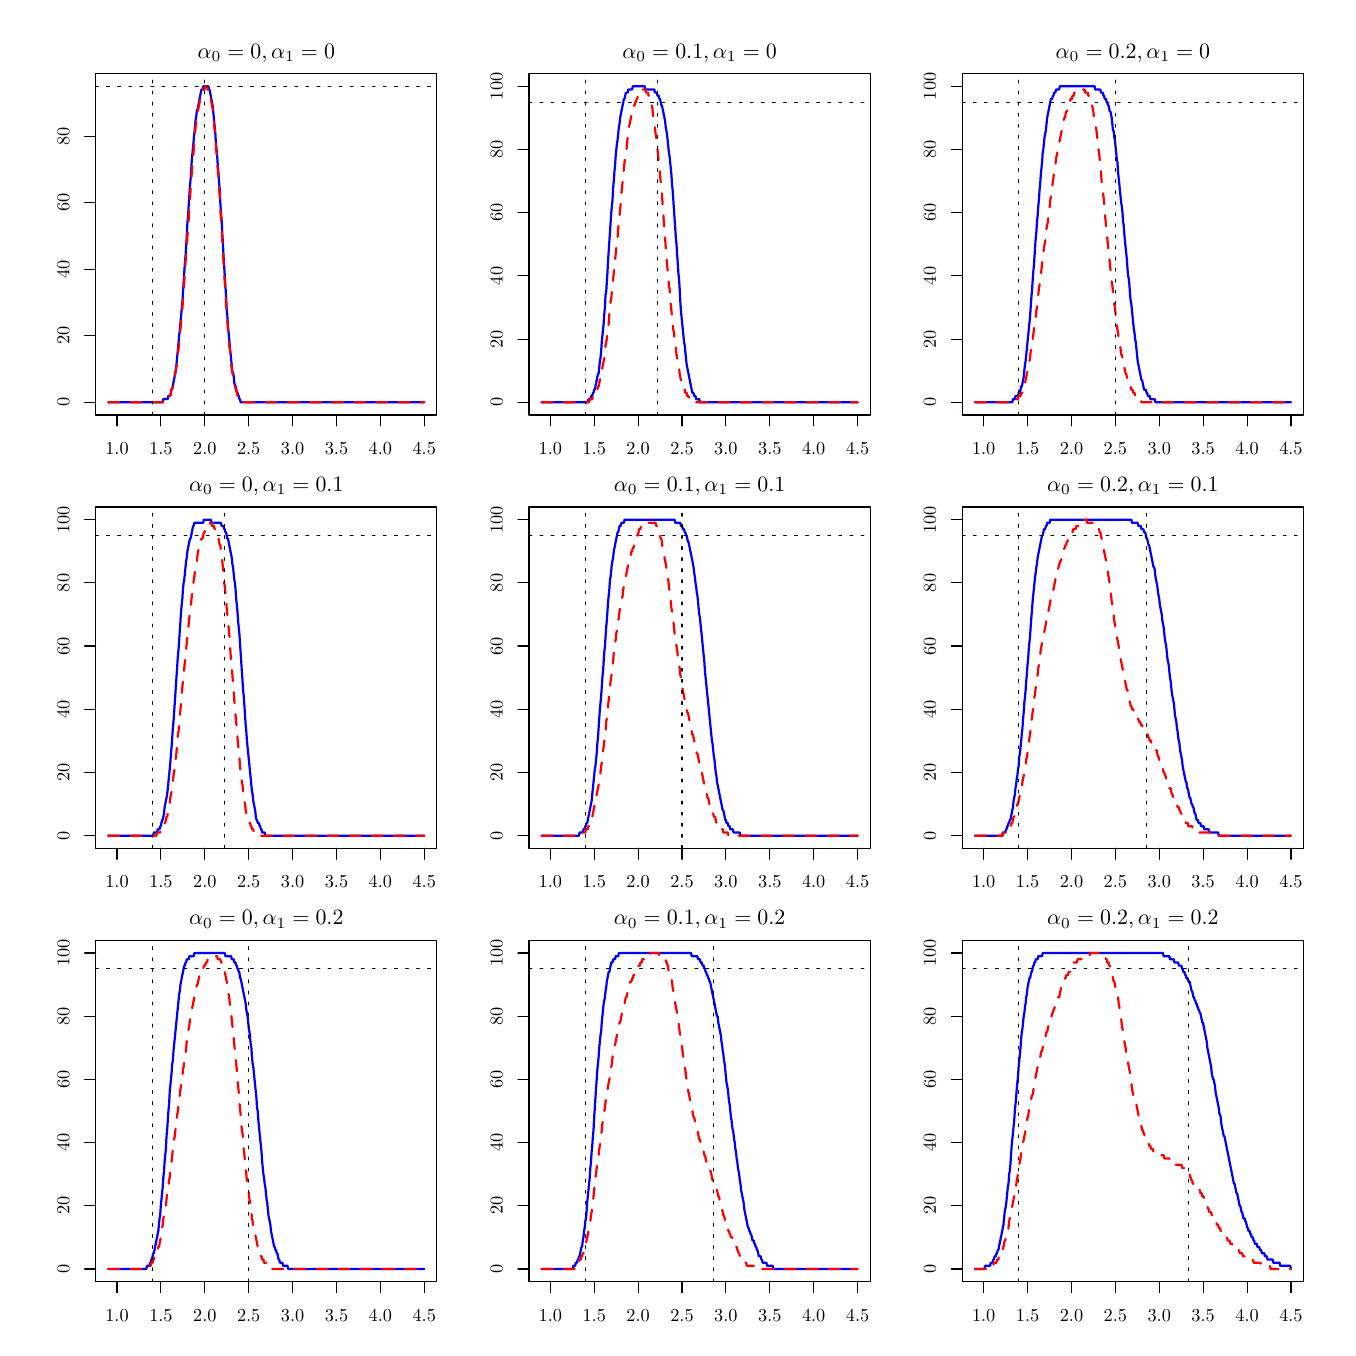
\begin{tikzpicture}[x=1pt,y=1pt]
\definecolor{fillColor}{RGB}{255,255,255}
\path[use as bounding box,fill=fillColor,fill opacity=0.00] (0,0) rectangle (469.75,469.75);
\begin{scope}
\path[clip] ( 24.55,329.80) rectangle (147.87,453.12);
\definecolor{drawColor}{RGB}{0,0,255}

\path[draw=drawColor,line width= 0.8pt,line join=round,line cap=round] ( 29.12,334.37) --
	( 29.35,334.37) --
	( 29.58,334.37) --
	( 29.81,334.37) --
	( 30.03,334.37) --
	( 30.26,334.37) --
	( 30.49,334.37) --
	( 30.72,334.37) --
	( 30.95,334.37) --
	( 31.18,334.37) --
	( 31.41,334.37) --
	( 31.64,334.37) --
	( 31.87,334.37) --
	( 32.09,334.37) --
	( 32.32,334.37) --
	( 32.55,334.37) --
	( 32.78,334.37) --
	( 33.01,334.37) --
	( 33.24,334.37) --
	( 33.47,334.37) --
	( 33.70,334.37) --
	( 33.92,334.37) --
	( 34.15,334.37) --
	( 34.38,334.37) --
	( 34.61,334.37) --
	( 34.84,334.37) --
	( 35.07,334.37) --
	( 35.30,334.37) --
	( 35.53,334.37) --
	( 35.76,334.37) --
	( 35.98,334.37) --
	( 36.21,334.37) --
	( 36.44,334.37) --
	( 36.67,334.37) --
	( 36.90,334.37) --
	( 37.13,334.37) --
	( 37.36,334.37) --
	( 37.59,334.37) --
	( 37.81,334.37) --
	( 38.04,334.37) --
	( 38.27,334.37) --
	( 38.50,334.37) --
	( 38.73,334.37) --
	( 38.96,334.37) --
	( 39.19,334.37) --
	( 39.42,334.37) --
	( 39.65,334.37) --
	( 39.87,334.37) --
	( 40.10,334.37) --
	( 40.33,334.37) --
	( 40.56,334.37) --
	( 40.79,334.37) --
	( 41.02,334.37) --
	( 41.25,334.37) --
	( 41.48,334.37) --
	( 41.71,334.37) --
	( 41.93,334.37) --
	( 42.16,334.37) --
	( 42.39,334.37) --
	( 42.62,334.37) --
	( 42.85,334.37) --
	( 43.08,334.37) --
	( 43.31,334.37) --
	( 43.54,334.37) --
	( 43.76,334.37) --
	( 43.99,334.37) --
	( 44.22,334.37) --
	( 44.45,334.37) --
	( 44.68,334.37) --
	( 44.91,334.37) --
	( 45.14,334.37) --
	( 45.37,334.37) --
	( 45.60,334.37) --
	( 45.82,334.37) --
	( 46.05,334.37) --
	( 46.28,334.37) --
	( 46.51,334.37) --
	( 46.74,334.37) --
	( 46.97,334.37) --
	( 47.20,334.37) --
	( 47.43,334.37) --
	( 47.65,334.37) --
	( 47.88,334.37) --
	( 48.11,334.37) --
	( 48.34,334.37) --
	( 48.57,334.37) --
	( 48.80,334.37) --
	( 49.03,335.57) --
	( 49.26,335.57) --
	( 49.49,335.57) --
	( 49.71,335.57) --
	( 49.94,335.57) --
	( 50.17,335.57) --
	( 50.40,335.57) --
	( 50.63,335.57) --
	( 50.86,336.77) --
	( 51.09,336.77) --
	( 51.32,336.77) --
	( 51.54,336.77) --
	( 51.77,337.98) --
	( 52.00,339.18) --
	( 52.23,339.18) --
	( 52.46,340.38) --
	( 52.69,341.58) --
	( 52.92,342.78) --
	( 53.15,343.99) --
	( 53.38,345.19) --
	( 53.60,346.39) --
	( 53.83,348.79) --
	( 54.06,351.20) --
	( 54.29,353.60) --
	( 54.52,356.00) --
	( 54.75,358.41) --
	( 54.98,360.81) --
	( 55.21,363.22) --
	( 55.43,365.62) --
	( 55.66,368.02) --
	( 55.89,370.43) --
	( 56.12,374.03) --
	( 56.35,377.64) --
	( 56.58,381.25) --
	( 56.81,384.85) --
	( 57.04,387.26) --
	( 57.27,390.86) --
	( 57.49,394.47) --
	( 57.72,399.28) --
	( 57.95,401.68) --
	( 58.18,405.29) --
	( 58.41,408.89) --
	( 58.64,412.50) --
	( 58.87,414.90) --
	( 59.10,418.51) --
	( 59.32,422.11) --
	( 59.55,424.52) --
	( 59.78,426.92) --
	( 60.01,429.32) --
	( 60.24,431.73) --
	( 60.47,434.13) --
	( 60.70,436.54) --
	( 60.93,437.74) --
	( 61.16,440.14) --
	( 61.38,440.14) --
	( 61.61,441.34) --
	( 61.84,442.55) --
	( 62.07,443.75) --
	( 62.30,444.95) --
	( 62.53,446.15) --
	( 62.76,447.35) --
	( 62.99,447.35) --
	( 63.22,447.35) --
	( 63.44,448.56) --
	( 63.67,448.56) --
	( 63.90,448.56) --
	( 64.13,448.56) --
	( 64.36,448.56) --
	( 64.59,448.56) --
	( 64.82,448.56) --
	( 65.05,448.56) --
	( 65.27,448.56) --
	( 65.50,447.35) --
	( 65.73,447.35) --
	( 65.96,446.15) --
	( 66.19,444.95) --
	( 66.42,443.75) --
	( 66.65,442.55) --
	( 66.88,441.34) --
	( 67.11,438.94) --
	( 67.33,436.54) --
	( 67.56,434.13) --
	( 67.79,431.73) --
	( 68.02,428.12) --
	( 68.25,425.72) --
	( 68.48,423.31) --
	( 68.71,419.71) --
	( 68.94,417.30) --
	( 69.16,413.70) --
	( 69.39,411.29) --
	( 69.62,406.49) --
	( 69.85,402.88) --
	( 70.08,400.48) --
	( 70.31,395.67) --
	( 70.54,392.06) --
	( 70.77,387.26) --
	( 71.00,383.65) --
	( 71.22,380.04) --
	( 71.45,376.44) --
	( 71.68,372.83) --
	( 71.91,368.02) --
	( 72.14,365.62) --
	( 72.37,362.01) --
	( 72.60,359.61) --
	( 72.83,357.21) --
	( 73.05,354.80) --
	( 73.28,352.40) --
	( 73.51,349.99) --
	( 73.74,347.59) --
	( 73.97,345.19) --
	( 74.20,345.19) --
	( 74.43,343.99) --
	( 74.66,341.58) --
	( 74.89,340.38) --
	( 75.11,340.38) --
	( 75.34,339.18) --
	( 75.57,337.98) --
	( 75.80,337.98) --
	( 76.03,336.77) --
	( 76.26,336.77) --
	( 76.49,335.57) --
	( 76.72,335.57) --
	( 76.94,334.37) --
	( 77.17,334.37) --
	( 77.40,334.37) --
	( 77.63,334.37) --
	( 77.86,334.37) --
	( 78.09,334.37) --
	( 78.32,334.37) --
	( 78.55,334.37) --
	( 78.78,334.37) --
	( 79.00,334.37) --
	( 79.23,334.37) --
	( 79.46,334.37) --
	( 79.69,334.37) --
	( 79.92,334.37) --
	( 80.15,334.37) --
	( 80.38,334.37) --
	( 80.61,334.37) --
	( 80.83,334.37) --
	( 81.06,334.37) --
	( 81.29,334.37) --
	( 81.52,334.37) --
	( 81.75,334.37) --
	( 81.98,334.37) --
	( 82.21,334.37) --
	( 82.44,334.37) --
	( 82.67,334.37) --
	( 82.89,334.37) --
	( 83.12,334.37) --
	( 83.35,334.37) --
	( 83.58,334.37) --
	( 83.81,334.37) --
	( 84.04,334.37) --
	( 84.27,334.37) --
	( 84.50,334.37) --
	( 84.73,334.37) --
	( 84.95,334.37) --
	( 85.18,334.37) --
	( 85.41,334.37) --
	( 85.64,334.37) --
	( 85.87,334.37) --
	( 86.10,334.37) --
	( 86.33,334.37) --
	( 86.56,334.37) --
	( 86.78,334.37) --
	( 87.01,334.37) --
	( 87.24,334.37) --
	( 87.47,334.37) --
	( 87.70,334.37) --
	( 87.93,334.37) --
	( 88.16,334.37) --
	( 88.39,334.37) --
	( 88.62,334.37) --
	( 88.84,334.37) --
	( 89.07,334.37) --
	( 89.30,334.37) --
	( 89.53,334.37) --
	( 89.76,334.37) --
	( 89.99,334.37) --
	( 90.22,334.37) --
	( 90.45,334.37) --
	( 90.67,334.37) --
	( 90.90,334.37) --
	( 91.13,334.37) --
	( 91.36,334.37) --
	( 91.59,334.37) --
	( 91.82,334.37) --
	( 92.05,334.37) --
	( 92.28,334.37) --
	( 92.51,334.37) --
	( 92.73,334.37) --
	( 92.96,334.37) --
	( 93.19,334.37) --
	( 93.42,334.37) --
	( 93.65,334.37) --
	( 93.88,334.37) --
	( 94.11,334.37) --
	( 94.34,334.37) --
	( 94.56,334.37) --
	( 94.79,334.37) --
	( 95.02,334.37) --
	( 95.25,334.37) --
	( 95.48,334.37) --
	( 95.71,334.37) --
	( 95.94,334.37) --
	( 96.17,334.37) --
	( 96.40,334.37) --
	( 96.62,334.37) --
	( 96.85,334.37) --
	( 97.08,334.37) --
	( 97.31,334.37) --
	( 97.54,334.37) --
	( 97.77,334.37) --
	( 98.00,334.37) --
	( 98.23,334.37) --
	( 98.45,334.37) --
	( 98.68,334.37) --
	( 98.91,334.37) --
	( 99.14,334.37) --
	( 99.37,334.37) --
	( 99.60,334.37) --
	( 99.83,334.37) --
	(100.06,334.37) --
	(100.29,334.37) --
	(100.51,334.37) --
	(100.74,334.37) --
	(100.97,334.37) --
	(101.20,334.37) --
	(101.43,334.37) --
	(101.66,334.37) --
	(101.89,334.37) --
	(102.12,334.37) --
	(102.35,334.37) --
	(102.57,334.37) --
	(102.80,334.37) --
	(103.03,334.37) --
	(103.26,334.37) --
	(103.49,334.37) --
	(103.72,334.37) --
	(103.95,334.37) --
	(104.18,334.37) --
	(104.40,334.37) --
	(104.63,334.37) --
	(104.86,334.37) --
	(105.09,334.37) --
	(105.32,334.37) --
	(105.55,334.37) --
	(105.78,334.37) --
	(106.01,334.37) --
	(106.24,334.37) --
	(106.46,334.37) --
	(106.69,334.37) --
	(106.92,334.37) --
	(107.15,334.37) --
	(107.38,334.37) --
	(107.61,334.37) --
	(107.84,334.37) --
	(108.07,334.37) --
	(108.29,334.37) --
	(108.52,334.37) --
	(108.75,334.37) --
	(108.98,334.37) --
	(109.21,334.37) --
	(109.44,334.37) --
	(109.67,334.37) --
	(109.90,334.37) --
	(110.13,334.37) --
	(110.35,334.37) --
	(110.58,334.37) --
	(110.81,334.37) --
	(111.04,334.37) --
	(111.27,334.37) --
	(111.50,334.37) --
	(111.73,334.37) --
	(111.96,334.37) --
	(112.18,334.37) --
	(112.41,334.37) --
	(112.64,334.37) --
	(112.87,334.37) --
	(113.10,334.37) --
	(113.33,334.37) --
	(113.56,334.37) --
	(113.79,334.37) --
	(114.02,334.37) --
	(114.24,334.37) --
	(114.47,334.37) --
	(114.70,334.37) --
	(114.93,334.37) --
	(115.16,334.37) --
	(115.39,334.37) --
	(115.62,334.37) --
	(115.85,334.37) --
	(116.07,334.37) --
	(116.30,334.37) --
	(116.53,334.37) --
	(116.76,334.37) --
	(116.99,334.37) --
	(117.22,334.37) --
	(117.45,334.37) --
	(117.68,334.37) --
	(117.91,334.37) --
	(118.13,334.37) --
	(118.36,334.37) --
	(118.59,334.37) --
	(118.82,334.37) --
	(119.05,334.37) --
	(119.28,334.37) --
	(119.51,334.37) --
	(119.74,334.37) --
	(119.96,334.37) --
	(120.19,334.37) --
	(120.42,334.37) --
	(120.65,334.37) --
	(120.88,334.37) --
	(121.11,334.37) --
	(121.34,334.37) --
	(121.57,334.37) --
	(121.80,334.37) --
	(122.02,334.37) --
	(122.25,334.37) --
	(122.48,334.37) --
	(122.71,334.37) --
	(122.94,334.37) --
	(123.17,334.37) --
	(123.40,334.37) --
	(123.63,334.37) --
	(123.86,334.37) --
	(124.08,334.37) --
	(124.31,334.37) --
	(124.54,334.37) --
	(124.77,334.37) --
	(125.00,334.37) --
	(125.23,334.37) --
	(125.46,334.37) --
	(125.69,334.37) --
	(125.91,334.37) --
	(126.14,334.37) --
	(126.37,334.37) --
	(126.60,334.37) --
	(126.83,334.37) --
	(127.06,334.37) --
	(127.29,334.37) --
	(127.52,334.37) --
	(127.75,334.37) --
	(127.97,334.37) --
	(128.20,334.37) --
	(128.43,334.37) --
	(128.66,334.37) --
	(128.89,334.37) --
	(129.12,334.37) --
	(129.35,334.37) --
	(129.58,334.37) --
	(129.80,334.37) --
	(130.03,334.37) --
	(130.26,334.37) --
	(130.49,334.37) --
	(130.72,334.37) --
	(130.95,334.37) --
	(131.18,334.37) --
	(131.41,334.37) --
	(131.64,334.37) --
	(131.86,334.37) --
	(132.09,334.37) --
	(132.32,334.37) --
	(132.55,334.37) --
	(132.78,334.37) --
	(133.01,334.37) --
	(133.24,334.37) --
	(133.47,334.37) --
	(133.69,334.37) --
	(133.92,334.37) --
	(134.15,334.37) --
	(134.38,334.37) --
	(134.61,334.37) --
	(134.84,334.37) --
	(135.07,334.37) --
	(135.30,334.37) --
	(135.53,334.37) --
	(135.75,334.37) --
	(135.98,334.37) --
	(136.21,334.37) --
	(136.44,334.37) --
	(136.67,334.37) --
	(136.90,334.37) --
	(137.13,334.37) --
	(137.36,334.37) --
	(137.58,334.37) --
	(137.81,334.37) --
	(138.04,334.37) --
	(138.27,334.37) --
	(138.50,334.37) --
	(138.73,334.37) --
	(138.96,334.37) --
	(139.19,334.37) --
	(139.42,334.37) --
	(139.64,334.37) --
	(139.87,334.37) --
	(140.10,334.37) --
	(140.33,334.37) --
	(140.56,334.37) --
	(140.79,334.37) --
	(141.02,334.37) --
	(141.25,334.37) --
	(141.47,334.37) --
	(141.70,334.37) --
	(141.93,334.37) --
	(142.16,334.37) --
	(142.39,334.37) --
	(142.62,334.37) --
	(142.85,334.37) --
	(143.08,334.37) --
	(143.31,334.37);
\end{scope}
\begin{scope}
\path[clip] (  0.00,  0.00) rectangle (469.75,469.75);
\definecolor{drawColor}{RGB}{0,0,0}

\path[draw=drawColor,line width= 0.4pt,line join=round,line cap=round] ( 32.29,329.80) -- (143.31,329.80);

\path[draw=drawColor,line width= 0.4pt,line join=round,line cap=round] ( 32.29,329.80) -- ( 32.29,325.84);

\path[draw=drawColor,line width= 0.4pt,line join=round,line cap=round] ( 48.15,329.80) -- ( 48.15,325.84);

\path[draw=drawColor,line width= 0.4pt,line join=round,line cap=round] ( 64.01,329.80) -- ( 64.01,325.84);

\path[draw=drawColor,line width= 0.4pt,line join=round,line cap=round] ( 79.87,329.80) -- ( 79.87,325.84);

\path[draw=drawColor,line width= 0.4pt,line join=round,line cap=round] ( 95.73,329.80) -- ( 95.73,325.84);

\path[draw=drawColor,line width= 0.4pt,line join=round,line cap=round] (111.59,329.80) -- (111.59,325.84);

\path[draw=drawColor,line width= 0.4pt,line join=round,line cap=round] (127.45,329.80) -- (127.45,325.84);

\path[draw=drawColor,line width= 0.4pt,line join=round,line cap=round] (143.31,329.80) -- (143.31,325.84);

\node[text=drawColor,anchor=base,inner sep=0pt, outer sep=0pt, scale=  0.66] at ( 32.29,315.55) {1.0};

\node[text=drawColor,anchor=base,inner sep=0pt, outer sep=0pt, scale=  0.66] at ( 48.15,315.55) {1.5};

\node[text=drawColor,anchor=base,inner sep=0pt, outer sep=0pt, scale=  0.66] at ( 64.01,315.55) {2.0};

\node[text=drawColor,anchor=base,inner sep=0pt, outer sep=0pt, scale=  0.66] at ( 79.87,315.55) {2.5};

\node[text=drawColor,anchor=base,inner sep=0pt, outer sep=0pt, scale=  0.66] at ( 95.73,315.55) {3.0};

\node[text=drawColor,anchor=base,inner sep=0pt, outer sep=0pt, scale=  0.66] at (111.59,315.55) {3.5};

\node[text=drawColor,anchor=base,inner sep=0pt, outer sep=0pt, scale=  0.66] at (127.45,315.55) {4.0};

\node[text=drawColor,anchor=base,inner sep=0pt, outer sep=0pt, scale=  0.66] at (143.31,315.55) {4.5};

\path[draw=drawColor,line width= 0.4pt,line join=round,line cap=round] ( 24.55,334.37) -- ( 24.55,430.53);

\path[draw=drawColor,line width= 0.4pt,line join=round,line cap=round] ( 24.55,334.37) -- ( 20.59,334.37);

\path[draw=drawColor,line width= 0.4pt,line join=round,line cap=round] ( 24.55,358.41) -- ( 20.59,358.41);

\path[draw=drawColor,line width= 0.4pt,line join=round,line cap=round] ( 24.55,382.45) -- ( 20.59,382.45);

\path[draw=drawColor,line width= 0.4pt,line join=round,line cap=round] ( 24.55,406.49) -- ( 20.59,406.49);

\path[draw=drawColor,line width= 0.4pt,line join=round,line cap=round] ( 24.55,430.53) -- ( 20.59,430.53);

\node[text=drawColor,rotate= 90.00,anchor=base,inner sep=0pt, outer sep=0pt, scale=  0.66] at ( 15.05,334.37) {0};

\node[text=drawColor,rotate= 90.00,anchor=base,inner sep=0pt, outer sep=0pt, scale=  0.66] at ( 15.05,358.41) {20};

\node[text=drawColor,rotate= 90.00,anchor=base,inner sep=0pt, outer sep=0pt, scale=  0.66] at ( 15.05,382.45) {40};

\node[text=drawColor,rotate= 90.00,anchor=base,inner sep=0pt, outer sep=0pt, scale=  0.66] at ( 15.05,406.49) {60};

\node[text=drawColor,rotate= 90.00,anchor=base,inner sep=0pt, outer sep=0pt, scale=  0.66] at ( 15.05,430.53) {80};

\path[draw=drawColor,line width= 0.4pt,line join=round,line cap=round] ( 24.55,329.80) --
	(147.87,329.80) --
	(147.87,453.12) --
	( 24.55,453.12) --
	( 24.55,329.80);
\end{scope}
\begin{scope}
\path[clip] (  0.00,313.17) rectangle (156.58,469.75);
\definecolor{drawColor}{RGB}{0,0,0}

\node[text=drawColor,anchor=base,inner sep=0pt, outer sep=0pt, scale=  0.79] at ( 86.21,458.71) {\bfseries $\alpha_0 = 0, \alpha_1 = 0$};
\end{scope}
\begin{scope}
\path[clip] ( 24.55,329.80) rectangle (147.87,453.12);
\definecolor{drawColor}{RGB}{255,0,0}

\path[draw=drawColor,line width= 0.8pt,dash pattern=on 4pt off 4pt ,line join=round,line cap=round] ( 29.12,334.37) --
	( 29.35,334.37) --
	( 29.58,334.37) --
	( 29.81,334.37) --
	( 30.03,334.37) --
	( 30.26,334.37) --
	( 30.49,334.37) --
	( 30.72,334.37) --
	( 30.95,334.37) --
	( 31.18,334.37) --
	( 31.41,334.37) --
	( 31.64,334.37) --
	( 31.87,334.37) --
	( 32.09,334.37) --
	( 32.32,334.37) --
	( 32.55,334.37) --
	( 32.78,334.37) --
	( 33.01,334.37) --
	( 33.24,334.37) --
	( 33.47,334.37) --
	( 33.70,334.37) --
	( 33.92,334.37) --
	( 34.15,334.37) --
	( 34.38,334.37) --
	( 34.61,334.37) --
	( 34.84,334.37) --
	( 35.07,334.37) --
	( 35.30,334.37) --
	( 35.53,334.37) --
	( 35.76,334.37) --
	( 35.98,334.37) --
	( 36.21,334.37) --
	( 36.44,334.37) --
	( 36.67,334.37) --
	( 36.90,334.37) --
	( 37.13,334.37) --
	( 37.36,334.37) --
	( 37.59,334.37) --
	( 37.81,334.37) --
	( 38.04,334.37) --
	( 38.27,334.37) --
	( 38.50,334.37) --
	( 38.73,334.37) --
	( 38.96,334.37) --
	( 39.19,334.37) --
	( 39.42,334.37) --
	( 39.65,334.37) --
	( 39.87,334.37) --
	( 40.10,334.37) --
	( 40.33,334.37) --
	( 40.56,334.37) --
	( 40.79,334.37) --
	( 41.02,334.37) --
	( 41.25,334.37) --
	( 41.48,334.37) --
	( 41.71,334.37) --
	( 41.93,334.37) --
	( 42.16,334.37) --
	( 42.39,334.37) --
	( 42.62,334.37) --
	( 42.85,334.37) --
	( 43.08,334.37) --
	( 43.31,334.37) --
	( 43.54,334.37) --
	( 43.76,334.37) --
	( 43.99,334.37) --
	( 44.22,334.37) --
	( 44.45,334.37) --
	( 44.68,334.37) --
	( 44.91,334.37) --
	( 45.14,334.37) --
	( 45.37,334.37) --
	( 45.60,334.37) --
	( 45.82,334.37) --
	( 46.05,334.37) --
	( 46.28,334.37) --
	( 46.51,334.37) --
	( 46.74,334.37) --
	( 46.97,334.37) --
	( 47.20,334.37) --
	( 47.43,334.37) --
	( 47.65,334.37) --
	( 47.88,334.37) --
	( 48.11,334.37) --
	( 48.34,334.37) --
	( 48.57,334.37) --
	( 48.80,334.37) --
	( 49.03,335.57) --
	( 49.26,335.57) --
	( 49.49,335.57) --
	( 49.71,335.57) --
	( 49.94,335.57) --
	( 50.17,335.57) --
	( 50.40,335.57) --
	( 50.63,335.57) --
	( 50.86,336.77) --
	( 51.09,336.77) --
	( 51.32,336.77) --
	( 51.54,336.77) --
	( 51.77,337.98) --
	( 52.00,339.18) --
	( 52.23,339.18) --
	( 52.46,340.38) --
	( 52.69,341.58) --
	( 52.92,342.78) --
	( 53.15,343.99) --
	( 53.38,345.19) --
	( 53.60,346.39) --
	( 53.83,347.59) --
	( 54.06,348.79) --
	( 54.29,352.40) --
	( 54.52,353.60) --
	( 54.75,356.00) --
	( 54.98,358.41) --
	( 55.21,360.81) --
	( 55.43,363.22) --
	( 55.66,365.62) --
	( 55.89,368.02) --
	( 56.12,371.63) --
	( 56.35,375.24) --
	( 56.58,377.64) --
	( 56.81,381.25) --
	( 57.04,384.85) --
	( 57.27,388.46) --
	( 57.49,390.86) --
	( 57.72,394.47) --
	( 57.95,396.87) --
	( 58.18,400.48) --
	( 58.41,405.29) --
	( 58.64,407.69) --
	( 58.87,411.29) --
	( 59.10,414.90) --
	( 59.32,417.30) --
	( 59.55,420.91) --
	( 59.78,423.31) --
	( 60.01,425.72) --
	( 60.24,429.32) --
	( 60.47,431.73) --
	( 60.70,434.13) --
	( 60.93,435.33) --
	( 61.16,437.74) --
	( 61.38,438.94) --
	( 61.61,440.14) --
	( 61.84,441.34) --
	( 62.07,442.55) --
	( 62.30,443.75) --
	( 62.53,444.95) --
	( 62.76,446.15) --
	( 62.99,446.15) --
	( 63.22,447.35) --
	( 63.44,447.35) --
	( 63.67,447.35) --
	( 63.90,447.35) --
	( 64.13,448.56) --
	( 64.36,448.56) --
	( 64.59,448.56) --
	( 64.82,448.56) --
	( 65.05,447.35) --
	( 65.27,447.35) --
	( 65.50,446.15) --
	( 65.73,446.15) --
	( 65.96,444.95) --
	( 66.19,443.75) --
	( 66.42,442.55) --
	( 66.65,441.34) --
	( 66.88,440.14) --
	( 67.11,437.74) --
	( 67.33,435.33) --
	( 67.56,432.93) --
	( 67.79,430.53) --
	( 68.02,426.92) --
	( 68.25,424.52) --
	( 68.48,420.91) --
	( 68.71,418.51) --
	( 68.94,414.90) --
	( 69.16,412.50) --
	( 69.39,408.89) --
	( 69.62,404.08) --
	( 69.85,400.48) --
	( 70.08,396.87) --
	( 70.31,393.27) --
	( 70.54,389.66) --
	( 70.77,384.85) --
	( 71.00,381.25) --
	( 71.22,377.64) --
	( 71.45,374.03) --
	( 71.68,370.43) --
	( 71.91,366.82) --
	( 72.14,364.42) --
	( 72.37,360.81) --
	( 72.60,358.41) --
	( 72.83,354.80) --
	( 73.05,353.60) --
	( 73.28,351.20) --
	( 73.51,348.79) --
	( 73.74,346.39) --
	( 73.97,345.19) --
	( 74.20,343.99) --
	( 74.43,342.78) --
	( 74.66,341.58) --
	( 74.89,340.38) --
	( 75.11,339.18) --
	( 75.34,339.18) --
	( 75.57,337.98) --
	( 75.80,336.77) --
	( 76.03,336.77) --
	( 76.26,335.57) --
	( 76.49,335.57) --
	( 76.72,335.57) --
	( 76.94,334.37) --
	( 77.17,334.37) --
	( 77.40,334.37) --
	( 77.63,334.37) --
	( 77.86,334.37) --
	( 78.09,334.37) --
	( 78.32,334.37) --
	( 78.55,334.37) --
	( 78.78,334.37) --
	( 79.00,334.37) --
	( 79.23,334.37) --
	( 79.46,334.37) --
	( 79.69,334.37) --
	( 79.92,334.37) --
	( 80.15,334.37) --
	( 80.38,334.37) --
	( 80.61,334.37) --
	( 80.83,334.37) --
	( 81.06,334.37) --
	( 81.29,334.37) --
	( 81.52,334.37) --
	( 81.75,334.37) --
	( 81.98,334.37) --
	( 82.21,334.37) --
	( 82.44,334.37) --
	( 82.67,334.37) --
	( 82.89,334.37) --
	( 83.12,334.37) --
	( 83.35,334.37) --
	( 83.58,334.37) --
	( 83.81,334.37) --
	( 84.04,334.37) --
	( 84.27,334.37) --
	( 84.50,334.37) --
	( 84.73,334.37) --
	( 84.95,334.37) --
	( 85.18,334.37) --
	( 85.41,334.37) --
	( 85.64,334.37) --
	( 85.87,334.37) --
	( 86.10,334.37) --
	( 86.33,334.37) --
	( 86.56,334.37) --
	( 86.78,334.37) --
	( 87.01,334.37) --
	( 87.24,334.37) --
	( 87.47,334.37) --
	( 87.70,334.37) --
	( 87.93,334.37) --
	( 88.16,334.37) --
	( 88.39,334.37) --
	( 88.62,334.37) --
	( 88.84,334.37) --
	( 89.07,334.37) --
	( 89.30,334.37) --
	( 89.53,334.37) --
	( 89.76,334.37) --
	( 89.99,334.37) --
	( 90.22,334.37) --
	( 90.45,334.37) --
	( 90.67,334.37) --
	( 90.90,334.37) --
	( 91.13,334.37) --
	( 91.36,334.37) --
	( 91.59,334.37) --
	( 91.82,334.37) --
	( 92.05,334.37) --
	( 92.28,334.37) --
	( 92.51,334.37) --
	( 92.73,334.37) --
	( 92.96,334.37) --
	( 93.19,334.37) --
	( 93.42,334.37) --
	( 93.65,334.37) --
	( 93.88,334.37) --
	( 94.11,334.37) --
	( 94.34,334.37) --
	( 94.56,334.37) --
	( 94.79,334.37) --
	( 95.02,334.37) --
	( 95.25,334.37) --
	( 95.48,334.37) --
	( 95.71,334.37) --
	( 95.94,334.37) --
	( 96.17,334.37) --
	( 96.40,334.37) --
	( 96.62,334.37) --
	( 96.85,334.37) --
	( 97.08,334.37) --
	( 97.31,334.37) --
	( 97.54,334.37) --
	( 97.77,334.37) --
	( 98.00,334.37) --
	( 98.23,334.37) --
	( 98.45,334.37) --
	( 98.68,334.37) --
	( 98.91,334.37) --
	( 99.14,334.37) --
	( 99.37,334.37) --
	( 99.60,334.37) --
	( 99.83,334.37) --
	(100.06,334.37) --
	(100.29,334.37) --
	(100.51,334.37) --
	(100.74,334.37) --
	(100.97,334.37) --
	(101.20,334.37) --
	(101.43,334.37) --
	(101.66,334.37) --
	(101.89,334.37) --
	(102.12,334.37) --
	(102.35,334.37) --
	(102.57,334.37) --
	(102.80,334.37) --
	(103.03,334.37) --
	(103.26,334.37) --
	(103.49,334.37) --
	(103.72,334.37) --
	(103.95,334.37) --
	(104.18,334.37) --
	(104.40,334.37) --
	(104.63,334.37) --
	(104.86,334.37) --
	(105.09,334.37) --
	(105.32,334.37) --
	(105.55,334.37) --
	(105.78,334.37) --
	(106.01,334.37) --
	(106.24,334.37) --
	(106.46,334.37) --
	(106.69,334.37) --
	(106.92,334.37) --
	(107.15,334.37) --
	(107.38,334.37) --
	(107.61,334.37) --
	(107.84,334.37) --
	(108.07,334.37) --
	(108.29,334.37) --
	(108.52,334.37) --
	(108.75,334.37) --
	(108.98,334.37) --
	(109.21,334.37) --
	(109.44,334.37) --
	(109.67,334.37) --
	(109.90,334.37) --
	(110.13,334.37) --
	(110.35,334.37) --
	(110.58,334.37) --
	(110.81,334.37) --
	(111.04,334.37) --
	(111.27,334.37) --
	(111.50,334.37) --
	(111.73,334.37) --
	(111.96,334.37) --
	(112.18,334.37) --
	(112.41,334.37) --
	(112.64,334.37) --
	(112.87,334.37) --
	(113.10,334.37) --
	(113.33,334.37) --
	(113.56,334.37) --
	(113.79,334.37) --
	(114.02,334.37) --
	(114.24,334.37) --
	(114.47,334.37) --
	(114.70,334.37) --
	(114.93,334.37) --
	(115.16,334.37) --
	(115.39,334.37) --
	(115.62,334.37) --
	(115.85,334.37) --
	(116.07,334.37) --
	(116.30,334.37) --
	(116.53,334.37) --
	(116.76,334.37) --
	(116.99,334.37) --
	(117.22,334.37) --
	(117.45,334.37) --
	(117.68,334.37) --
	(117.91,334.37) --
	(118.13,334.37) --
	(118.36,334.37) --
	(118.59,334.37) --
	(118.82,334.37) --
	(119.05,334.37) --
	(119.28,334.37) --
	(119.51,334.37) --
	(119.74,334.37) --
	(119.96,334.37) --
	(120.19,334.37) --
	(120.42,334.37) --
	(120.65,334.37) --
	(120.88,334.37) --
	(121.11,334.37) --
	(121.34,334.37) --
	(121.57,334.37) --
	(121.80,334.37) --
	(122.02,334.37) --
	(122.25,334.37) --
	(122.48,334.37) --
	(122.71,334.37) --
	(122.94,334.37) --
	(123.17,334.37) --
	(123.40,334.37) --
	(123.63,334.37) --
	(123.86,334.37) --
	(124.08,334.37) --
	(124.31,334.37) --
	(124.54,334.37) --
	(124.77,334.37) --
	(125.00,334.37) --
	(125.23,334.37) --
	(125.46,334.37) --
	(125.69,334.37) --
	(125.91,334.37) --
	(126.14,334.37) --
	(126.37,334.37) --
	(126.60,334.37) --
	(126.83,334.37) --
	(127.06,334.37) --
	(127.29,334.37) --
	(127.52,334.37) --
	(127.75,334.37) --
	(127.97,334.37) --
	(128.20,334.37) --
	(128.43,334.37) --
	(128.66,334.37) --
	(128.89,334.37) --
	(129.12,334.37) --
	(129.35,334.37) --
	(129.58,334.37) --
	(129.80,334.37) --
	(130.03,334.37) --
	(130.26,334.37) --
	(130.49,334.37) --
	(130.72,334.37) --
	(130.95,334.37) --
	(131.18,334.37) --
	(131.41,334.37) --
	(131.64,334.37) --
	(131.86,334.37) --
	(132.09,334.37) --
	(132.32,334.37) --
	(132.55,334.37) --
	(132.78,334.37) --
	(133.01,334.37) --
	(133.24,334.37) --
	(133.47,334.37) --
	(133.69,334.37) --
	(133.92,334.37) --
	(134.15,334.37) --
	(134.38,334.37) --
	(134.61,334.37) --
	(134.84,334.37) --
	(135.07,334.37) --
	(135.30,334.37) --
	(135.53,334.37) --
	(135.75,334.37) --
	(135.98,334.37) --
	(136.21,334.37) --
	(136.44,334.37) --
	(136.67,334.37) --
	(136.90,334.37) --
	(137.13,334.37) --
	(137.36,334.37) --
	(137.58,334.37) --
	(137.81,334.37) --
	(138.04,334.37) --
	(138.27,334.37) --
	(138.50,334.37) --
	(138.73,334.37) --
	(138.96,334.37) --
	(139.19,334.37) --
	(139.42,334.37) --
	(139.64,334.37) --
	(139.87,334.37) --
	(140.10,334.37) --
	(140.33,334.37) --
	(140.56,334.37) --
	(140.79,334.37) --
	(141.02,334.37) --
	(141.25,334.37) --
	(141.47,334.37) --
	(141.70,334.37) --
	(141.93,334.37) --
	(142.16,334.37) --
	(142.39,334.37) --
	(142.62,334.37) --
	(142.85,334.37) --
	(143.08,334.37) --
	(143.31,334.37);
\definecolor{drawColor}{RGB}{0,0,0}

\path[draw=drawColor,line width= 0.4pt,dash pattern=on 1pt off 3pt ,line join=round,line cap=round] ( 24.55,448.56) -- (147.87,448.56);

\path[draw=drawColor,line width= 0.4pt,dash pattern=on 1pt off 3pt ,line join=round,line cap=round] ( 44.98,329.80) -- ( 44.98,453.12);

\path[draw=drawColor,line width= 0.4pt,dash pattern=on 1pt off 3pt ,line join=round,line cap=round] ( 64.01,329.80) -- ( 64.01,453.12);
\end{scope}
\begin{scope}
\path[clip] (181.14,329.80) rectangle (304.46,453.12);
\definecolor{drawColor}{RGB}{0,0,255}

\path[draw=drawColor,line width= 0.8pt,line join=round,line cap=round] (185.70,334.37) --
	(185.93,334.37) --
	(186.16,334.37) --
	(186.39,334.37) --
	(186.62,334.37) --
	(186.85,334.37) --
	(187.08,334.37) --
	(187.31,334.37) --
	(187.54,334.37) --
	(187.76,334.37) --
	(187.99,334.37) --
	(188.22,334.37) --
	(188.45,334.37) --
	(188.68,334.37) --
	(188.91,334.37) --
	(189.14,334.37) --
	(189.37,334.37) --
	(189.59,334.37) --
	(189.82,334.37) --
	(190.05,334.37) --
	(190.28,334.37) --
	(190.51,334.37) --
	(190.74,334.37) --
	(190.97,334.37) --
	(191.20,334.37) --
	(191.43,334.37) --
	(191.65,334.37) --
	(191.88,334.37) --
	(192.11,334.37) --
	(192.34,334.37) --
	(192.57,334.37) --
	(192.80,334.37) --
	(193.03,334.37) --
	(193.26,334.37) --
	(193.48,334.37) --
	(193.71,334.37) --
	(193.94,334.37) --
	(194.17,334.37) --
	(194.40,334.37) --
	(194.63,334.37) --
	(194.86,334.37) --
	(195.09,334.37) --
	(195.32,334.37) --
	(195.54,334.37) --
	(195.77,334.37) --
	(196.00,334.37) --
	(196.23,334.37) --
	(196.46,334.37) --
	(196.69,334.37) --
	(196.92,334.37) --
	(197.15,334.37) --
	(197.37,334.37) --
	(197.60,334.37) --
	(197.83,334.37) --
	(198.06,334.37) --
	(198.29,334.37) --
	(198.52,334.37) --
	(198.75,334.37) --
	(198.98,334.37) --
	(199.21,334.37) --
	(199.43,334.37) --
	(199.66,334.37) --
	(199.89,334.37) --
	(200.12,334.37) --
	(200.35,334.37) --
	(200.58,334.37) --
	(200.81,334.37) --
	(201.04,334.37) --
	(201.26,334.37) --
	(201.49,334.37) --
	(201.72,334.37) --
	(201.95,334.37) --
	(202.18,334.37) --
	(202.41,334.37) --
	(202.64,335.51) --
	(202.87,335.51) --
	(203.10,335.51) --
	(203.32,335.51) --
	(203.55,336.65) --
	(203.78,336.65) --
	(204.01,336.65) --
	(204.24,337.80) --
	(204.47,337.80) --
	(204.70,338.94) --
	(204.93,338.94) --
	(205.15,340.08) --
	(205.38,341.22) --
	(205.61,342.36) --
	(205.84,343.50) --
	(206.07,344.65) --
	(206.30,344.65) --
	(206.53,346.93) --
	(206.76,349.21) --
	(206.99,350.36) --
	(207.21,352.64) --
	(207.44,356.06) --
	(207.67,358.35) --
	(207.90,360.63) --
	(208.13,362.92) --
	(208.36,366.34) --
	(208.59,368.63) --
	(208.82,373.19) --
	(209.05,374.33) --
	(209.27,377.76) --
	(209.50,381.19) --
	(209.73,385.75) --
	(209.96,389.18) --
	(210.19,392.60) --
	(210.42,396.03) --
	(210.65,399.46) --
	(210.88,402.88) --
	(211.10,405.16) --
	(211.33,407.45) --
	(211.56,412.02) --
	(211.79,414.30) --
	(212.02,417.73) --
	(212.25,420.01) --
	(212.48,423.43) --
	(212.71,425.72) --
	(212.94,428.00) --
	(213.16,429.14) --
	(213.39,431.43) --
	(213.62,433.71) --
	(213.85,434.85) --
	(214.08,437.14) --
	(214.31,438.28) --
	(214.54,439.42) --
	(214.77,440.56) --
	(214.99,441.70) --
	(215.22,442.85) --
	(215.45,443.99) --
	(215.68,443.99) --
	(215.91,445.13) --
	(216.14,446.27) --
	(216.37,446.27) --
	(216.60,446.27) --
	(216.83,446.27) --
	(217.05,447.41) --
	(217.28,447.41) --
	(217.51,447.41) --
	(217.74,447.41) --
	(217.97,447.41) --
	(218.20,447.41) --
	(218.43,447.41) --
	(218.66,448.56) --
	(218.88,448.56) --
	(219.11,448.56) --
	(219.34,448.56) --
	(219.57,448.56) --
	(219.80,448.56) --
	(220.03,448.56) --
	(220.26,448.56) --
	(220.49,448.56) --
	(220.72,448.56) --
	(220.94,448.56) --
	(221.17,448.56) --
	(221.40,448.56) --
	(221.63,448.56) --
	(221.86,448.56) --
	(222.09,448.56) --
	(222.32,448.56) --
	(222.55,448.56) --
	(222.77,448.56) --
	(223.00,448.56) --
	(223.23,447.41) --
	(223.46,447.41) --
	(223.69,447.41) --
	(223.92,447.41) --
	(224.15,447.41) --
	(224.38,447.41) --
	(224.61,447.41) --
	(224.83,447.41) --
	(225.06,447.41) --
	(225.29,447.41) --
	(225.52,447.41) --
	(225.75,447.41) --
	(225.98,447.41) --
	(226.21,447.41) --
	(226.44,447.41) --
	(226.66,446.27) --
	(226.89,446.27) --
	(227.12,446.27) --
	(227.35,446.27) --
	(227.58,445.13) --
	(227.81,445.13) --
	(228.04,445.13) --
	(228.27,443.99) --
	(228.50,443.99) --
	(228.72,442.85) --
	(228.95,441.70) --
	(229.18,441.70) --
	(229.41,440.56) --
	(229.64,439.42) --
	(229.87,438.28) --
	(230.10,437.14) --
	(230.33,436.00) --
	(230.56,433.71) --
	(230.78,432.57) --
	(231.01,431.43) --
	(231.24,429.14) --
	(231.47,426.86) --
	(231.70,424.58) --
	(231.93,423.43) --
	(232.16,421.15) --
	(232.39,418.87) --
	(232.61,416.58) --
	(232.84,413.16) --
	(233.07,410.87) --
	(233.30,407.45) --
	(233.53,404.02) --
	(233.76,400.60) --
	(233.99,397.17) --
	(234.22,393.75) --
	(234.45,391.46) --
	(234.67,388.04) --
	(234.90,384.61) --
	(235.13,381.19) --
	(235.36,378.90) --
	(235.59,375.48) --
	(235.82,370.91) --
	(236.05,367.48) --
	(236.28,365.20) --
	(236.50,362.92) --
	(236.73,360.63) --
	(236.96,358.35) --
	(237.19,356.06) --
	(237.42,354.92) --
	(237.65,352.64) --
	(237.88,350.36) --
	(238.11,348.07) --
	(238.34,346.93) --
	(238.56,345.79) --
	(238.79,344.65) --
	(239.02,343.50) --
	(239.25,342.36) --
	(239.48,341.22) --
	(239.71,340.08) --
	(239.94,338.94) --
	(240.17,337.80) --
	(240.39,337.80) --
	(240.62,337.80) --
	(240.85,336.65) --
	(241.08,336.65) --
	(241.31,336.65) --
	(241.54,335.51) --
	(241.77,335.51) --
	(242.00,335.51) --
	(242.23,335.51) --
	(242.45,335.51) --
	(242.68,335.51) --
	(242.91,334.37) --
	(243.14,334.37) --
	(243.37,334.37) --
	(243.60,334.37) --
	(243.83,334.37) --
	(244.06,334.37) --
	(244.28,334.37) --
	(244.51,334.37) --
	(244.74,334.37) --
	(244.97,334.37) --
	(245.20,334.37) --
	(245.43,334.37) --
	(245.66,334.37) --
	(245.89,334.37) --
	(246.12,334.37) --
	(246.34,334.37) --
	(246.57,334.37) --
	(246.80,334.37) --
	(247.03,334.37) --
	(247.26,334.37) --
	(247.49,334.37) --
	(247.72,334.37) --
	(247.95,334.37) --
	(248.18,334.37) --
	(248.40,334.37) --
	(248.63,334.37) --
	(248.86,334.37) --
	(249.09,334.37) --
	(249.32,334.37) --
	(249.55,334.37) --
	(249.78,334.37) --
	(250.01,334.37) --
	(250.23,334.37) --
	(250.46,334.37) --
	(250.69,334.37) --
	(250.92,334.37) --
	(251.15,334.37) --
	(251.38,334.37) --
	(251.61,334.37) --
	(251.84,334.37) --
	(252.07,334.37) --
	(252.29,334.37) --
	(252.52,334.37) --
	(252.75,334.37) --
	(252.98,334.37) --
	(253.21,334.37) --
	(253.44,334.37) --
	(253.67,334.37) --
	(253.90,334.37) --
	(254.12,334.37) --
	(254.35,334.37) --
	(254.58,334.37) --
	(254.81,334.37) --
	(255.04,334.37) --
	(255.27,334.37) --
	(255.50,334.37) --
	(255.73,334.37) --
	(255.96,334.37) --
	(256.18,334.37) --
	(256.41,334.37) --
	(256.64,334.37) --
	(256.87,334.37) --
	(257.10,334.37) --
	(257.33,334.37) --
	(257.56,334.37) --
	(257.79,334.37) --
	(258.01,334.37) --
	(258.24,334.37) --
	(258.47,334.37) --
	(258.70,334.37) --
	(258.93,334.37) --
	(259.16,334.37) --
	(259.39,334.37) --
	(259.62,334.37) --
	(259.85,334.37) --
	(260.07,334.37) --
	(260.30,334.37) --
	(260.53,334.37) --
	(260.76,334.37) --
	(260.99,334.37) --
	(261.22,334.37) --
	(261.45,334.37) --
	(261.68,334.37) --
	(261.90,334.37) --
	(262.13,334.37) --
	(262.36,334.37) --
	(262.59,334.37) --
	(262.82,334.37) --
	(263.05,334.37) --
	(263.28,334.37) --
	(263.51,334.37) --
	(263.74,334.37) --
	(263.96,334.37) --
	(264.19,334.37) --
	(264.42,334.37) --
	(264.65,334.37) --
	(264.88,334.37) --
	(265.11,334.37) --
	(265.34,334.37) --
	(265.57,334.37) --
	(265.79,334.37) --
	(266.02,334.37) --
	(266.25,334.37) --
	(266.48,334.37) --
	(266.71,334.37) --
	(266.94,334.37) --
	(267.17,334.37) --
	(267.40,334.37) --
	(267.63,334.37) --
	(267.85,334.37) --
	(268.08,334.37) --
	(268.31,334.37) --
	(268.54,334.37) --
	(268.77,334.37) --
	(269.00,334.37) --
	(269.23,334.37) --
	(269.46,334.37) --
	(269.69,334.37) --
	(269.91,334.37) --
	(270.14,334.37) --
	(270.37,334.37) --
	(270.60,334.37) --
	(270.83,334.37) --
	(271.06,334.37) --
	(271.29,334.37) --
	(271.52,334.37) --
	(271.74,334.37) --
	(271.97,334.37) --
	(272.20,334.37) --
	(272.43,334.37) --
	(272.66,334.37) --
	(272.89,334.37) --
	(273.12,334.37) --
	(273.35,334.37) --
	(273.58,334.37) --
	(273.80,334.37) --
	(274.03,334.37) --
	(274.26,334.37) --
	(274.49,334.37) --
	(274.72,334.37) --
	(274.95,334.37) --
	(275.18,334.37) --
	(275.41,334.37) --
	(275.63,334.37) --
	(275.86,334.37) --
	(276.09,334.37) --
	(276.32,334.37) --
	(276.55,334.37) --
	(276.78,334.37) --
	(277.01,334.37) --
	(277.24,334.37) --
	(277.47,334.37) --
	(277.69,334.37) --
	(277.92,334.37) --
	(278.15,334.37) --
	(278.38,334.37) --
	(278.61,334.37) --
	(278.84,334.37) --
	(279.07,334.37) --
	(279.30,334.37) --
	(279.52,334.37) --
	(279.75,334.37) --
	(279.98,334.37) --
	(280.21,334.37) --
	(280.44,334.37) --
	(280.67,334.37) --
	(280.90,334.37) --
	(281.13,334.37) --
	(281.36,334.37) --
	(281.58,334.37) --
	(281.81,334.37) --
	(282.04,334.37) --
	(282.27,334.37) --
	(282.50,334.37) --
	(282.73,334.37) --
	(282.96,334.37) --
	(283.19,334.37) --
	(283.41,334.37) --
	(283.64,334.37) --
	(283.87,334.37) --
	(284.10,334.37) --
	(284.33,334.37) --
	(284.56,334.37) --
	(284.79,334.37) --
	(285.02,334.37) --
	(285.25,334.37) --
	(285.47,334.37) --
	(285.70,334.37) --
	(285.93,334.37) --
	(286.16,334.37) --
	(286.39,334.37) --
	(286.62,334.37) --
	(286.85,334.37) --
	(287.08,334.37) --
	(287.30,334.37) --
	(287.53,334.37) --
	(287.76,334.37) --
	(287.99,334.37) --
	(288.22,334.37) --
	(288.45,334.37) --
	(288.68,334.37) --
	(288.91,334.37) --
	(289.14,334.37) --
	(289.36,334.37) --
	(289.59,334.37) --
	(289.82,334.37) --
	(290.05,334.37) --
	(290.28,334.37) --
	(290.51,334.37) --
	(290.74,334.37) --
	(290.97,334.37) --
	(291.20,334.37) --
	(291.42,334.37) --
	(291.65,334.37) --
	(291.88,334.37) --
	(292.11,334.37) --
	(292.34,334.37) --
	(292.57,334.37) --
	(292.80,334.37) --
	(293.03,334.37) --
	(293.25,334.37) --
	(293.48,334.37) --
	(293.71,334.37) --
	(293.94,334.37) --
	(294.17,334.37) --
	(294.40,334.37) --
	(294.63,334.37) --
	(294.86,334.37) --
	(295.09,334.37) --
	(295.31,334.37) --
	(295.54,334.37) --
	(295.77,334.37) --
	(296.00,334.37) --
	(296.23,334.37) --
	(296.46,334.37) --
	(296.69,334.37) --
	(296.92,334.37) --
	(297.14,334.37) --
	(297.37,334.37) --
	(297.60,334.37) --
	(297.83,334.37) --
	(298.06,334.37) --
	(298.29,334.37) --
	(298.52,334.37) --
	(298.75,334.37) --
	(298.98,334.37) --
	(299.20,334.37) --
	(299.43,334.37) --
	(299.66,334.37) --
	(299.89,334.37);
\end{scope}
\begin{scope}
\path[clip] (  0.00,  0.00) rectangle (469.75,469.75);
\definecolor{drawColor}{RGB}{0,0,0}

\path[draw=drawColor,line width= 0.4pt,line join=round,line cap=round] (188.88,329.80) -- (299.89,329.80);

\path[draw=drawColor,line width= 0.4pt,line join=round,line cap=round] (188.88,329.80) -- (188.88,325.84);

\path[draw=drawColor,line width= 0.4pt,line join=round,line cap=round] (204.74,329.80) -- (204.74,325.84);

\path[draw=drawColor,line width= 0.4pt,line join=round,line cap=round] (220.59,329.80) -- (220.59,325.84);

\path[draw=drawColor,line width= 0.4pt,line join=round,line cap=round] (236.45,329.80) -- (236.45,325.84);

\path[draw=drawColor,line width= 0.4pt,line join=round,line cap=round] (252.31,329.80) -- (252.31,325.84);

\path[draw=drawColor,line width= 0.4pt,line join=round,line cap=round] (268.17,329.80) -- (268.17,325.84);

\path[draw=drawColor,line width= 0.4pt,line join=round,line cap=round] (284.03,329.80) -- (284.03,325.84);

\path[draw=drawColor,line width= 0.4pt,line join=round,line cap=round] (299.89,329.80) -- (299.89,325.84);

\node[text=drawColor,anchor=base,inner sep=0pt, outer sep=0pt, scale=  0.66] at (188.88,315.55) {1.0};

\node[text=drawColor,anchor=base,inner sep=0pt, outer sep=0pt, scale=  0.66] at (204.74,315.55) {1.5};

\node[text=drawColor,anchor=base,inner sep=0pt, outer sep=0pt, scale=  0.66] at (220.59,315.55) {2.0};

\node[text=drawColor,anchor=base,inner sep=0pt, outer sep=0pt, scale=  0.66] at (236.45,315.55) {2.5};

\node[text=drawColor,anchor=base,inner sep=0pt, outer sep=0pt, scale=  0.66] at (252.31,315.55) {3.0};

\node[text=drawColor,anchor=base,inner sep=0pt, outer sep=0pt, scale=  0.66] at (268.17,315.55) {3.5};

\node[text=drawColor,anchor=base,inner sep=0pt, outer sep=0pt, scale=  0.66] at (284.03,315.55) {4.0};

\node[text=drawColor,anchor=base,inner sep=0pt, outer sep=0pt, scale=  0.66] at (299.89,315.55) {4.5};

\path[draw=drawColor,line width= 0.4pt,line join=round,line cap=round] (181.14,334.37) -- (181.14,448.56);

\path[draw=drawColor,line width= 0.4pt,line join=round,line cap=round] (181.14,334.37) -- (177.18,334.37);

\path[draw=drawColor,line width= 0.4pt,line join=round,line cap=round] (181.14,357.21) -- (177.18,357.21);

\path[draw=drawColor,line width= 0.4pt,line join=round,line cap=round] (181.14,380.04) -- (177.18,380.04);

\path[draw=drawColor,line width= 0.4pt,line join=round,line cap=round] (181.14,402.88) -- (177.18,402.88);

\path[draw=drawColor,line width= 0.4pt,line join=round,line cap=round] (181.14,425.72) -- (177.18,425.72);

\path[draw=drawColor,line width= 0.4pt,line join=round,line cap=round] (181.14,448.56) -- (177.18,448.56);

\node[text=drawColor,rotate= 90.00,anchor=base,inner sep=0pt, outer sep=0pt, scale=  0.66] at (171.63,334.37) {0};

\node[text=drawColor,rotate= 90.00,anchor=base,inner sep=0pt, outer sep=0pt, scale=  0.66] at (171.63,357.21) {20};

\node[text=drawColor,rotate= 90.00,anchor=base,inner sep=0pt, outer sep=0pt, scale=  0.66] at (171.63,380.04) {40};

\node[text=drawColor,rotate= 90.00,anchor=base,inner sep=0pt, outer sep=0pt, scale=  0.66] at (171.63,402.88) {60};

\node[text=drawColor,rotate= 90.00,anchor=base,inner sep=0pt, outer sep=0pt, scale=  0.66] at (171.63,425.72) {80};

\node[text=drawColor,rotate= 90.00,anchor=base,inner sep=0pt, outer sep=0pt, scale=  0.66] at (171.63,448.56) {100};

\path[draw=drawColor,line width= 0.4pt,line join=round,line cap=round] (181.14,329.80) --
	(304.46,329.80) --
	(304.46,453.12) --
	(181.14,453.12) --
	(181.14,329.80);
\end{scope}
\begin{scope}
\path[clip] (156.58,313.17) rectangle (313.17,469.75);
\definecolor{drawColor}{RGB}{0,0,0}

\node[text=drawColor,anchor=base,inner sep=0pt, outer sep=0pt, scale=  0.79] at (242.80,458.71) {\bfseries $\alpha_0 = 0.1, \alpha_1 = 0$};
\end{scope}
\begin{scope}
\path[clip] (181.14,329.80) rectangle (304.46,453.12);
\definecolor{drawColor}{RGB}{255,0,0}

\path[draw=drawColor,line width= 0.8pt,dash pattern=on 4pt off 4pt ,line join=round,line cap=round] (185.70,334.37) --
	(185.93,334.37) --
	(186.16,334.37) --
	(186.39,334.37) --
	(186.62,334.37) --
	(186.85,334.37) --
	(187.08,334.37) --
	(187.31,334.37) --
	(187.54,334.37) --
	(187.76,334.37) --
	(187.99,334.37) --
	(188.22,334.37) --
	(188.45,334.37) --
	(188.68,334.37) --
	(188.91,334.37) --
	(189.14,334.37) --
	(189.37,334.37) --
	(189.59,334.37) --
	(189.82,334.37) --
	(190.05,334.37) --
	(190.28,334.37) --
	(190.51,334.37) --
	(190.74,334.37) --
	(190.97,334.37) --
	(191.20,334.37) --
	(191.43,334.37) --
	(191.65,334.37) --
	(191.88,334.37) --
	(192.11,334.37) --
	(192.34,334.37) --
	(192.57,334.37) --
	(192.80,334.37) --
	(193.03,334.37) --
	(193.26,334.37) --
	(193.48,334.37) --
	(193.71,334.37) --
	(193.94,334.37) --
	(194.17,334.37) --
	(194.40,334.37) --
	(194.63,334.37) --
	(194.86,334.37) --
	(195.09,334.37) --
	(195.32,334.37) --
	(195.54,334.37) --
	(195.77,334.37) --
	(196.00,334.37) --
	(196.23,334.37) --
	(196.46,334.37) --
	(196.69,334.37) --
	(196.92,334.37) --
	(197.15,334.37) --
	(197.37,334.37) --
	(197.60,334.37) --
	(197.83,334.37) --
	(198.06,334.37) --
	(198.29,334.37) --
	(198.52,334.37) --
	(198.75,334.37) --
	(198.98,334.37) --
	(199.21,334.37) --
	(199.43,334.37) --
	(199.66,334.37) --
	(199.89,334.37) --
	(200.12,334.37) --
	(200.35,334.37) --
	(200.58,334.37) --
	(200.81,334.37) --
	(201.04,334.37) --
	(201.26,334.37) --
	(201.49,334.37) --
	(201.72,334.37) --
	(201.95,334.37) --
	(202.18,334.37) --
	(202.41,334.37) --
	(202.64,334.37) --
	(202.87,334.37) --
	(203.10,335.51) --
	(203.32,335.51) --
	(203.55,335.51) --
	(203.78,335.51) --
	(204.01,335.51) --
	(204.24,336.65) --
	(204.47,336.65) --
	(204.70,336.65) --
	(204.93,336.65) --
	(205.15,336.65) --
	(205.38,337.80) --
	(205.61,337.80) --
	(205.84,338.94) --
	(206.07,340.08) --
	(206.30,340.08) --
	(206.53,341.22) --
	(206.76,342.36) --
	(206.99,343.50) --
	(207.21,343.50) --
	(207.44,344.65) --
	(207.67,346.93) --
	(207.90,348.07) --
	(208.13,349.21) --
	(208.36,350.36) --
	(208.59,352.64) --
	(208.82,354.92) --
	(209.05,356.06) --
	(209.27,357.21) --
	(209.50,359.49) --
	(209.73,360.63) --
	(209.96,362.92) --
	(210.19,366.34) --
	(210.42,368.63) --
	(210.65,370.91) --
	(210.88,372.05) --
	(211.10,374.33) --
	(211.33,376.62) --
	(211.56,378.90) --
	(211.79,381.19) --
	(212.02,383.47) --
	(212.25,385.75) --
	(212.48,388.04) --
	(212.71,390.32) --
	(212.94,392.60) --
	(213.16,393.75) --
	(213.39,397.17) --
	(213.62,399.46) --
	(213.85,401.74) --
	(214.08,404.02) --
	(214.31,406.31) --
	(214.54,409.73) --
	(214.77,412.02) --
	(214.99,414.30) --
	(215.22,416.58) --
	(215.45,418.87) --
	(215.68,421.15) --
	(215.91,423.43) --
	(216.14,424.58) --
	(216.37,425.72) --
	(216.60,428.00) --
	(216.83,430.29) --
	(217.05,431.43) --
	(217.28,433.71) --
	(217.51,434.85) --
	(217.74,436.00) --
	(217.97,437.14) --
	(218.20,438.28) --
	(218.43,438.28) --
	(218.66,439.42) --
	(218.88,440.56) --
	(219.11,441.70) --
	(219.34,441.70) --
	(219.57,442.85) --
	(219.80,442.85) --
	(220.03,443.99) --
	(220.26,443.99) --
	(220.49,445.13) --
	(220.72,446.27) --
	(220.94,446.27) --
	(221.17,446.27) --
	(221.40,446.27) --
	(221.63,447.41) --
	(221.86,447.41) --
	(222.09,447.41) --
	(222.32,447.41) --
	(222.55,447.41) --
	(222.77,447.41) --
	(223.00,447.41) --
	(223.23,447.41) --
	(223.46,446.27) --
	(223.69,446.27) --
	(223.92,446.27) --
	(224.15,446.27) --
	(224.38,445.13) --
	(224.61,443.99) --
	(224.83,443.99) --
	(225.06,442.85) --
	(225.29,442.85) --
	(225.52,441.70) --
	(225.75,440.56) --
	(225.98,438.28) --
	(226.21,437.14) --
	(226.44,434.85) --
	(226.66,433.71) --
	(226.89,431.43) --
	(227.12,430.29) --
	(227.35,428.00) --
	(227.58,425.72) --
	(227.81,423.43) --
	(228.04,421.15) --
	(228.27,420.01) --
	(228.50,416.58) --
	(228.72,414.30) --
	(228.95,412.02) --
	(229.18,409.73) --
	(229.41,406.31) --
	(229.64,402.88) --
	(229.87,399.46) --
	(230.10,397.17) --
	(230.33,393.75) --
	(230.56,390.32) --
	(230.78,386.90) --
	(231.01,384.61) --
	(231.24,382.33) --
	(231.47,380.04) --
	(231.70,376.62) --
	(231.93,375.48) --
	(232.16,373.19) --
	(232.39,369.77) --
	(232.61,367.48) --
	(232.84,365.20) --
	(233.07,362.92) --
	(233.30,360.63) --
	(233.53,359.49) --
	(233.76,357.21) --
	(233.99,356.06) --
	(234.22,353.78) --
	(234.45,351.50) --
	(234.67,350.36) --
	(234.90,349.21) --
	(235.13,348.07) --
	(235.36,346.93) --
	(235.59,344.65) --
	(235.82,343.50) --
	(236.05,342.36) --
	(236.28,342.36) --
	(236.50,341.22) --
	(236.73,341.22) --
	(236.96,340.08) --
	(237.19,338.94) --
	(237.42,338.94) --
	(237.65,337.80) --
	(237.88,337.80) --
	(238.11,337.80) --
	(238.34,336.65) --
	(238.56,336.65) --
	(238.79,336.65) --
	(239.02,335.51) --
	(239.25,335.51) --
	(239.48,335.51) --
	(239.71,335.51) --
	(239.94,335.51) --
	(240.17,334.37) --
	(240.39,334.37) --
	(240.62,334.37) --
	(240.85,334.37) --
	(241.08,334.37) --
	(241.31,334.37) --
	(241.54,334.37) --
	(241.77,334.37) --
	(242.00,334.37) --
	(242.23,334.37) --
	(242.45,334.37) --
	(242.68,334.37) --
	(242.91,334.37) --
	(243.14,334.37) --
	(243.37,334.37) --
	(243.60,334.37) --
	(243.83,334.37) --
	(244.06,334.37) --
	(244.28,334.37) --
	(244.51,334.37) --
	(244.74,334.37) --
	(244.97,334.37) --
	(245.20,334.37) --
	(245.43,334.37) --
	(245.66,334.37) --
	(245.89,334.37) --
	(246.12,334.37) --
	(246.34,334.37) --
	(246.57,334.37) --
	(246.80,334.37) --
	(247.03,334.37) --
	(247.26,334.37) --
	(247.49,334.37) --
	(247.72,334.37) --
	(247.95,334.37) --
	(248.18,334.37) --
	(248.40,334.37) --
	(248.63,334.37) --
	(248.86,334.37) --
	(249.09,334.37) --
	(249.32,334.37) --
	(249.55,334.37) --
	(249.78,334.37) --
	(250.01,334.37) --
	(250.23,334.37) --
	(250.46,334.37) --
	(250.69,334.37) --
	(250.92,334.37) --
	(251.15,334.37) --
	(251.38,334.37) --
	(251.61,334.37) --
	(251.84,334.37) --
	(252.07,334.37) --
	(252.29,334.37) --
	(252.52,334.37) --
	(252.75,334.37) --
	(252.98,334.37) --
	(253.21,334.37) --
	(253.44,334.37) --
	(253.67,334.37) --
	(253.90,334.37) --
	(254.12,334.37) --
	(254.35,334.37) --
	(254.58,334.37) --
	(254.81,334.37) --
	(255.04,334.37) --
	(255.27,334.37) --
	(255.50,334.37) --
	(255.73,334.37) --
	(255.96,334.37) --
	(256.18,334.37) --
	(256.41,334.37) --
	(256.64,334.37) --
	(256.87,334.37) --
	(257.10,334.37) --
	(257.33,334.37) --
	(257.56,334.37) --
	(257.79,334.37) --
	(258.01,334.37) --
	(258.24,334.37) --
	(258.47,334.37) --
	(258.70,334.37) --
	(258.93,334.37) --
	(259.16,334.37) --
	(259.39,334.37) --
	(259.62,334.37) --
	(259.85,334.37) --
	(260.07,334.37) --
	(260.30,334.37) --
	(260.53,334.37) --
	(260.76,334.37) --
	(260.99,334.37) --
	(261.22,334.37) --
	(261.45,334.37) --
	(261.68,334.37) --
	(261.90,334.37) --
	(262.13,334.37) --
	(262.36,334.37) --
	(262.59,334.37) --
	(262.82,334.37) --
	(263.05,334.37) --
	(263.28,334.37) --
	(263.51,334.37) --
	(263.74,334.37) --
	(263.96,334.37) --
	(264.19,334.37) --
	(264.42,334.37) --
	(264.65,334.37) --
	(264.88,334.37) --
	(265.11,334.37) --
	(265.34,334.37) --
	(265.57,334.37) --
	(265.79,334.37) --
	(266.02,334.37) --
	(266.25,334.37) --
	(266.48,334.37) --
	(266.71,334.37) --
	(266.94,334.37) --
	(267.17,334.37) --
	(267.40,334.37) --
	(267.63,334.37) --
	(267.85,334.37) --
	(268.08,334.37) --
	(268.31,334.37) --
	(268.54,334.37) --
	(268.77,334.37) --
	(269.00,334.37) --
	(269.23,334.37) --
	(269.46,334.37) --
	(269.69,334.37) --
	(269.91,334.37) --
	(270.14,334.37) --
	(270.37,334.37) --
	(270.60,334.37) --
	(270.83,334.37) --
	(271.06,334.37) --
	(271.29,334.37) --
	(271.52,334.37) --
	(271.74,334.37) --
	(271.97,334.37) --
	(272.20,334.37) --
	(272.43,334.37) --
	(272.66,334.37) --
	(272.89,334.37) --
	(273.12,334.37) --
	(273.35,334.37) --
	(273.58,334.37) --
	(273.80,334.37) --
	(274.03,334.37) --
	(274.26,334.37) --
	(274.49,334.37) --
	(274.72,334.37) --
	(274.95,334.37) --
	(275.18,334.37) --
	(275.41,334.37) --
	(275.63,334.37) --
	(275.86,334.37) --
	(276.09,334.37) --
	(276.32,334.37) --
	(276.55,334.37) --
	(276.78,334.37) --
	(277.01,334.37) --
	(277.24,334.37) --
	(277.47,334.37) --
	(277.69,334.37) --
	(277.92,334.37) --
	(278.15,334.37) --
	(278.38,334.37) --
	(278.61,334.37) --
	(278.84,334.37) --
	(279.07,334.37) --
	(279.30,334.37) --
	(279.52,334.37) --
	(279.75,334.37) --
	(279.98,334.37) --
	(280.21,334.37) --
	(280.44,334.37) --
	(280.67,334.37) --
	(280.90,334.37) --
	(281.13,334.37) --
	(281.36,334.37) --
	(281.58,334.37) --
	(281.81,334.37) --
	(282.04,334.37) --
	(282.27,334.37) --
	(282.50,334.37) --
	(282.73,334.37) --
	(282.96,334.37) --
	(283.19,334.37) --
	(283.41,334.37) --
	(283.64,334.37) --
	(283.87,334.37) --
	(284.10,334.37) --
	(284.33,334.37) --
	(284.56,334.37) --
	(284.79,334.37) --
	(285.02,334.37) --
	(285.25,334.37) --
	(285.47,334.37) --
	(285.70,334.37) --
	(285.93,334.37) --
	(286.16,334.37) --
	(286.39,334.37) --
	(286.62,334.37) --
	(286.85,334.37) --
	(287.08,334.37) --
	(287.30,334.37) --
	(287.53,334.37) --
	(287.76,334.37) --
	(287.99,334.37) --
	(288.22,334.37) --
	(288.45,334.37) --
	(288.68,334.37) --
	(288.91,334.37) --
	(289.14,334.37) --
	(289.36,334.37) --
	(289.59,334.37) --
	(289.82,334.37) --
	(290.05,334.37) --
	(290.28,334.37) --
	(290.51,334.37) --
	(290.74,334.37) --
	(290.97,334.37) --
	(291.20,334.37) --
	(291.42,334.37) --
	(291.65,334.37) --
	(291.88,334.37) --
	(292.11,334.37) --
	(292.34,334.37) --
	(292.57,334.37) --
	(292.80,334.37) --
	(293.03,334.37) --
	(293.25,334.37) --
	(293.48,334.37) --
	(293.71,334.37) --
	(293.94,334.37) --
	(294.17,334.37) --
	(294.40,334.37) --
	(294.63,334.37) --
	(294.86,334.37) --
	(295.09,334.37) --
	(295.31,334.37) --
	(295.54,334.37) --
	(295.77,334.37) --
	(296.00,334.37) --
	(296.23,334.37) --
	(296.46,334.37) --
	(296.69,334.37) --
	(296.92,334.37) --
	(297.14,334.37) --
	(297.37,334.37) --
	(297.60,334.37) --
	(297.83,334.37) --
	(298.06,334.37) --
	(298.29,334.37) --
	(298.52,334.37) --
	(298.75,334.37) --
	(298.98,334.37) --
	(299.20,334.37) --
	(299.43,334.37) --
	(299.66,334.37) --
	(299.89,334.37);
\definecolor{drawColor}{RGB}{0,0,0}

\path[draw=drawColor,line width= 0.4pt,dash pattern=on 1pt off 3pt ,line join=round,line cap=round] (181.14,442.85) -- (304.46,442.85);

\path[draw=drawColor,line width= 0.4pt,dash pattern=on 1pt off 3pt ,line join=round,line cap=round] (201.56,329.80) -- (201.56,453.12);

\path[draw=drawColor,line width= 0.4pt,dash pattern=on 1pt off 3pt ,line join=round,line cap=round] (227.64,329.80) -- (227.64,453.12);
\end{scope}
\begin{scope}
\path[clip] (337.72,329.80) rectangle (461.04,453.12);
\definecolor{drawColor}{RGB}{0,0,255}

\path[draw=drawColor,line width= 0.8pt,line join=round,line cap=round] (342.29,334.37) --
	(342.52,334.37) --
	(342.75,334.37) --
	(342.98,334.37) --
	(343.20,334.37) --
	(343.43,334.37) --
	(343.66,334.37) --
	(343.89,334.37) --
	(344.12,334.37) --
	(344.35,334.37) --
	(344.58,334.37) --
	(344.81,334.37) --
	(345.04,334.37) --
	(345.26,334.37) --
	(345.49,334.37) --
	(345.72,334.37) --
	(345.95,334.37) --
	(346.18,334.37) --
	(346.41,334.37) --
	(346.64,334.37) --
	(346.87,334.37) --
	(347.09,334.37) --
	(347.32,334.37) --
	(347.55,334.37) --
	(347.78,334.37) --
	(348.01,334.37) --
	(348.24,334.37) --
	(348.47,334.37) --
	(348.70,334.37) --
	(348.93,334.37) --
	(349.15,334.37) --
	(349.38,334.37) --
	(349.61,334.37) --
	(349.84,334.37) --
	(350.07,334.37) --
	(350.30,334.37) --
	(350.53,334.37) --
	(350.76,334.37) --
	(350.98,334.37) --
	(351.21,334.37) --
	(351.44,334.37) --
	(351.67,334.37) --
	(351.90,334.37) --
	(352.13,334.37) --
	(352.36,334.37) --
	(352.59,334.37) --
	(352.82,334.37) --
	(353.04,334.37) --
	(353.27,334.37) --
	(353.50,334.37) --
	(353.73,334.37) --
	(353.96,334.37) --
	(354.19,334.37) --
	(354.42,334.37) --
	(354.65,334.37) --
	(354.88,334.37) --
	(355.10,334.37) --
	(355.33,334.37) --
	(355.56,334.37) --
	(355.79,334.37) --
	(356.02,335.51) --
	(356.25,335.51) --
	(356.48,335.51) --
	(356.71,335.51) --
	(356.93,336.65) --
	(357.16,336.65) --
	(357.39,336.65) --
	(357.62,336.65) --
	(357.85,336.65) --
	(358.08,337.80) --
	(358.31,337.80) --
	(358.54,337.80) --
	(358.77,338.94) --
	(358.99,340.08) --
	(359.22,340.08) --
	(359.45,341.22) --
	(359.68,342.36) --
	(359.91,343.50) --
	(360.14,345.79) --
	(360.37,348.07) --
	(360.60,349.21) --
	(360.82,351.50) --
	(361.05,353.78) --
	(361.28,356.06) --
	(361.51,358.35) --
	(361.74,360.63) --
	(361.97,362.92) --
	(362.20,365.20) --
	(362.43,368.63) --
	(362.66,372.05) --
	(362.88,374.33) --
	(363.11,377.76) --
	(363.34,381.19) --
	(363.57,383.47) --
	(363.80,386.90) --
	(364.03,390.32) --
	(364.26,393.75) --
	(364.49,396.03) --
	(364.71,399.46) --
	(364.94,401.74) --
	(365.17,405.16) --
	(365.40,407.45) --
	(365.63,410.87) --
	(365.86,413.16) --
	(366.09,416.58) --
	(366.32,418.87) --
	(366.55,421.15) --
	(366.77,424.58) --
	(367.00,425.72) --
	(367.23,428.00) --
	(367.46,430.29) --
	(367.69,431.43) --
	(367.92,432.57) --
	(368.15,434.85) --
	(368.38,437.14) --
	(368.60,438.28) --
	(368.83,439.42) --
	(369.06,440.56) --
	(369.29,441.70) --
	(369.52,442.85) --
	(369.75,443.99) --
	(369.98,443.99) --
	(370.21,443.99) --
	(370.44,445.13) --
	(370.66,445.13) --
	(370.89,446.27) --
	(371.12,446.27) --
	(371.35,446.27) --
	(371.58,447.41) --
	(371.81,447.41) --
	(372.04,447.41) --
	(372.27,447.41) --
	(372.49,447.41) --
	(372.72,447.41) --
	(372.95,448.56) --
	(373.18,448.56) --
	(373.41,448.56) --
	(373.64,448.56) --
	(373.87,448.56) --
	(374.10,448.56) --
	(374.33,448.56) --
	(374.55,448.56) --
	(374.78,448.56) --
	(375.01,448.56) --
	(375.24,448.56) --
	(375.47,448.56) --
	(375.70,448.56) --
	(375.93,448.56) --
	(376.16,448.56) --
	(376.39,448.56) --
	(376.61,448.56) --
	(376.84,448.56) --
	(377.07,448.56) --
	(377.30,448.56) --
	(377.53,448.56) --
	(377.76,448.56) --
	(377.99,448.56) --
	(378.22,448.56) --
	(378.44,448.56) --
	(378.67,448.56) --
	(378.90,448.56) --
	(379.13,448.56) --
	(379.36,448.56) --
	(379.59,448.56) --
	(379.82,448.56) --
	(380.05,448.56) --
	(380.28,448.56) --
	(380.50,448.56) --
	(380.73,448.56) --
	(380.96,448.56) --
	(381.19,448.56) --
	(381.42,448.56) --
	(381.65,448.56) --
	(381.88,448.56) --
	(382.11,448.56) --
	(382.33,448.56) --
	(382.56,448.56) --
	(382.79,448.56) --
	(383.02,448.56) --
	(383.25,448.56) --
	(383.48,448.56) --
	(383.71,448.56) --
	(383.94,448.56) --
	(384.17,448.56) --
	(384.39,448.56) --
	(384.62,448.56) --
	(384.85,448.56) --
	(385.08,448.56) --
	(385.31,448.56) --
	(385.54,448.56) --
	(385.77,447.41) --
	(386.00,447.41) --
	(386.22,447.41) --
	(386.45,447.41) --
	(386.68,447.41) --
	(386.91,447.41) --
	(387.14,447.41) --
	(387.37,447.41) --
	(387.60,447.41) --
	(387.83,446.27) --
	(388.06,446.27) --
	(388.28,446.27) --
	(388.51,446.27) --
	(388.74,445.13) --
	(388.97,445.13) --
	(389.20,443.99) --
	(389.43,443.99) --
	(389.66,443.99) --
	(389.89,442.85) --
	(390.11,442.85) --
	(390.34,441.70) --
	(390.57,441.70) --
	(390.80,440.56) --
	(391.03,439.42) --
	(391.26,439.42) --
	(391.49,438.28) --
	(391.72,437.14) --
	(391.95,434.85) --
	(392.17,432.57) --
	(392.40,432.57) --
	(392.63,430.29) --
	(392.86,429.14) --
	(393.09,426.86) --
	(393.32,424.58) --
	(393.55,422.29) --
	(393.78,421.15) --
	(394.00,417.73) --
	(394.23,415.44) --
	(394.46,413.16) --
	(394.69,410.87) --
	(394.92,408.59) --
	(395.15,406.31) --
	(395.38,405.16) --
	(395.61,402.88) --
	(395.84,399.46) --
	(396.06,398.31) --
	(396.29,394.89) --
	(396.52,392.60) --
	(396.75,390.32) --
	(396.98,388.04) --
	(397.21,385.75) --
	(397.44,382.33) --
	(397.67,380.04) --
	(397.90,378.90) --
	(398.12,376.62) --
	(398.35,373.19) --
	(398.58,370.91) --
	(398.81,369.77) --
	(399.04,367.48) --
	(399.27,365.20) --
	(399.50,362.92) --
	(399.73,360.63) --
	(399.95,359.49) --
	(400.18,357.21) --
	(400.41,356.06) --
	(400.64,353.78) --
	(400.87,351.50) --
	(401.10,349.21) --
	(401.33,348.07) --
	(401.56,346.93) --
	(401.79,345.79) --
	(402.01,344.65) --
	(402.24,343.50) --
	(402.47,342.36) --
	(402.70,342.36) --
	(402.93,341.22) --
	(403.16,340.08) --
	(403.39,338.94) --
	(403.62,338.94) --
	(403.84,338.94) --
	(404.07,338.94) --
	(404.30,337.80) --
	(404.53,337.80) --
	(404.76,336.65) --
	(404.99,336.65) --
	(405.22,336.65) --
	(405.45,336.65) --
	(405.68,335.51) --
	(405.90,335.51) --
	(406.13,335.51) --
	(406.36,335.51) --
	(406.59,335.51) --
	(406.82,335.51) --
	(407.05,335.51) --
	(407.28,335.51) --
	(407.51,334.37) --
	(407.73,334.37) --
	(407.96,334.37) --
	(408.19,334.37) --
	(408.42,334.37) --
	(408.65,334.37) --
	(408.88,334.37) --
	(409.11,334.37) --
	(409.34,334.37) --
	(409.57,334.37) --
	(409.79,334.37) --
	(410.02,334.37) --
	(410.25,334.37) --
	(410.48,334.37) --
	(410.71,334.37) --
	(410.94,334.37) --
	(411.17,334.37) --
	(411.40,334.37) --
	(411.62,334.37) --
	(411.85,334.37) --
	(412.08,334.37) --
	(412.31,334.37) --
	(412.54,334.37) --
	(412.77,334.37) --
	(413.00,334.37) --
	(413.23,334.37) --
	(413.46,334.37) --
	(413.68,334.37) --
	(413.91,334.37) --
	(414.14,334.37) --
	(414.37,334.37) --
	(414.60,334.37) --
	(414.83,334.37) --
	(415.06,334.37) --
	(415.29,334.37) --
	(415.52,334.37) --
	(415.74,334.37) --
	(415.97,334.37) --
	(416.20,334.37) --
	(416.43,334.37) --
	(416.66,334.37) --
	(416.89,334.37) --
	(417.12,334.37) --
	(417.35,334.37) --
	(417.57,334.37) --
	(417.80,334.37) --
	(418.03,334.37) --
	(418.26,334.37) --
	(418.49,334.37) --
	(418.72,334.37) --
	(418.95,334.37) --
	(419.18,334.37) --
	(419.41,334.37) --
	(419.63,334.37) --
	(419.86,334.37) --
	(420.09,334.37) --
	(420.32,334.37) --
	(420.55,334.37) --
	(420.78,334.37) --
	(421.01,334.37) --
	(421.24,334.37) --
	(421.46,334.37) --
	(421.69,334.37) --
	(421.92,334.37) --
	(422.15,334.37) --
	(422.38,334.37) --
	(422.61,334.37) --
	(422.84,334.37) --
	(423.07,334.37) --
	(423.30,334.37) --
	(423.52,334.37) --
	(423.75,334.37) --
	(423.98,334.37) --
	(424.21,334.37) --
	(424.44,334.37) --
	(424.67,334.37) --
	(424.90,334.37) --
	(425.13,334.37) --
	(425.35,334.37) --
	(425.58,334.37) --
	(425.81,334.37) --
	(426.04,334.37) --
	(426.27,334.37) --
	(426.50,334.37) --
	(426.73,334.37) --
	(426.96,334.37) --
	(427.19,334.37) --
	(427.41,334.37) --
	(427.64,334.37) --
	(427.87,334.37) --
	(428.10,334.37) --
	(428.33,334.37) --
	(428.56,334.37) --
	(428.79,334.37) --
	(429.02,334.37) --
	(429.24,334.37) --
	(429.47,334.37) --
	(429.70,334.37) --
	(429.93,334.37) --
	(430.16,334.37) --
	(430.39,334.37) --
	(430.62,334.37) --
	(430.85,334.37) --
	(431.08,334.37) --
	(431.30,334.37) --
	(431.53,334.37) --
	(431.76,334.37) --
	(431.99,334.37) --
	(432.22,334.37) --
	(432.45,334.37) --
	(432.68,334.37) --
	(432.91,334.37) --
	(433.13,334.37) --
	(433.36,334.37) --
	(433.59,334.37) --
	(433.82,334.37) --
	(434.05,334.37) --
	(434.28,334.37) --
	(434.51,334.37) --
	(434.74,334.37) --
	(434.97,334.37) --
	(435.19,334.37) --
	(435.42,334.37) --
	(435.65,334.37) --
	(435.88,334.37) --
	(436.11,334.37) --
	(436.34,334.37) --
	(436.57,334.37) --
	(436.80,334.37) --
	(437.03,334.37) --
	(437.25,334.37) --
	(437.48,334.37) --
	(437.71,334.37) --
	(437.94,334.37) --
	(438.17,334.37) --
	(438.40,334.37) --
	(438.63,334.37) --
	(438.86,334.37) --
	(439.08,334.37) --
	(439.31,334.37) --
	(439.54,334.37) --
	(439.77,334.37) --
	(440.00,334.37) --
	(440.23,334.37) --
	(440.46,334.37) --
	(440.69,334.37) --
	(440.92,334.37) --
	(441.14,334.37) --
	(441.37,334.37) --
	(441.60,334.37) --
	(441.83,334.37) --
	(442.06,334.37) --
	(442.29,334.37) --
	(442.52,334.37) --
	(442.75,334.37) --
	(442.97,334.37) --
	(443.20,334.37) --
	(443.43,334.37) --
	(443.66,334.37) --
	(443.89,334.37) --
	(444.12,334.37) --
	(444.35,334.37) --
	(444.58,334.37) --
	(444.81,334.37) --
	(445.03,334.37) --
	(445.26,334.37) --
	(445.49,334.37) --
	(445.72,334.37) --
	(445.95,334.37) --
	(446.18,334.37) --
	(446.41,334.37) --
	(446.64,334.37) --
	(446.86,334.37) --
	(447.09,334.37) --
	(447.32,334.37) --
	(447.55,334.37) --
	(447.78,334.37) --
	(448.01,334.37) --
	(448.24,334.37) --
	(448.47,334.37) --
	(448.70,334.37) --
	(448.92,334.37) --
	(449.15,334.37) --
	(449.38,334.37) --
	(449.61,334.37) --
	(449.84,334.37) --
	(450.07,334.37) --
	(450.30,334.37) --
	(450.53,334.37) --
	(450.75,334.37) --
	(450.98,334.37) --
	(451.21,334.37) --
	(451.44,334.37) --
	(451.67,334.37) --
	(451.90,334.37) --
	(452.13,334.37) --
	(452.36,334.37) --
	(452.59,334.37) --
	(452.81,334.37) --
	(453.04,334.37) --
	(453.27,334.37) --
	(453.50,334.37) --
	(453.73,334.37) --
	(453.96,334.37) --
	(454.19,334.37) --
	(454.42,334.37) --
	(454.64,334.37) --
	(454.87,334.37) --
	(455.10,334.37) --
	(455.33,334.37) --
	(455.56,334.37) --
	(455.79,334.37) --
	(456.02,334.37) --
	(456.25,334.37) --
	(456.48,334.37);
\end{scope}
\begin{scope}
\path[clip] (  0.00,  0.00) rectangle (469.75,469.75);
\definecolor{drawColor}{RGB}{0,0,0}

\path[draw=drawColor,line width= 0.4pt,line join=round,line cap=round] (345.46,329.80) -- (456.48,329.80);

\path[draw=drawColor,line width= 0.4pt,line join=round,line cap=round] (345.46,329.80) -- (345.46,325.84);

\path[draw=drawColor,line width= 0.4pt,line join=round,line cap=round] (361.32,329.80) -- (361.32,325.84);

\path[draw=drawColor,line width= 0.4pt,line join=round,line cap=round] (377.18,329.80) -- (377.18,325.84);

\path[draw=drawColor,line width= 0.4pt,line join=round,line cap=round] (393.04,329.80) -- (393.04,325.84);

\path[draw=drawColor,line width= 0.4pt,line join=round,line cap=round] (408.90,329.80) -- (408.90,325.84);

\path[draw=drawColor,line width= 0.4pt,line join=round,line cap=round] (424.76,329.80) -- (424.76,325.84);

\path[draw=drawColor,line width= 0.4pt,line join=round,line cap=round] (440.62,329.80) -- (440.62,325.84);

\path[draw=drawColor,line width= 0.4pt,line join=round,line cap=round] (456.48,329.80) -- (456.48,325.84);

\node[text=drawColor,anchor=base,inner sep=0pt, outer sep=0pt, scale=  0.66] at (345.46,315.55) {1.0};

\node[text=drawColor,anchor=base,inner sep=0pt, outer sep=0pt, scale=  0.66] at (361.32,315.55) {1.5};

\node[text=drawColor,anchor=base,inner sep=0pt, outer sep=0pt, scale=  0.66] at (377.18,315.55) {2.0};

\node[text=drawColor,anchor=base,inner sep=0pt, outer sep=0pt, scale=  0.66] at (393.04,315.55) {2.5};

\node[text=drawColor,anchor=base,inner sep=0pt, outer sep=0pt, scale=  0.66] at (408.90,315.55) {3.0};

\node[text=drawColor,anchor=base,inner sep=0pt, outer sep=0pt, scale=  0.66] at (424.76,315.55) {3.5};

\node[text=drawColor,anchor=base,inner sep=0pt, outer sep=0pt, scale=  0.66] at (440.62,315.55) {4.0};

\node[text=drawColor,anchor=base,inner sep=0pt, outer sep=0pt, scale=  0.66] at (456.48,315.55) {4.5};

\path[draw=drawColor,line width= 0.4pt,line join=round,line cap=round] (337.72,334.37) -- (337.72,448.56);

\path[draw=drawColor,line width= 0.4pt,line join=round,line cap=round] (337.72,334.37) -- (333.76,334.37);

\path[draw=drawColor,line width= 0.4pt,line join=round,line cap=round] (337.72,357.21) -- (333.76,357.21);

\path[draw=drawColor,line width= 0.4pt,line join=round,line cap=round] (337.72,380.04) -- (333.76,380.04);

\path[draw=drawColor,line width= 0.4pt,line join=round,line cap=round] (337.72,402.88) -- (333.76,402.88);

\path[draw=drawColor,line width= 0.4pt,line join=round,line cap=round] (337.72,425.72) -- (333.76,425.72);

\path[draw=drawColor,line width= 0.4pt,line join=round,line cap=round] (337.72,448.56) -- (333.76,448.56);

\node[text=drawColor,rotate= 90.00,anchor=base,inner sep=0pt, outer sep=0pt, scale=  0.66] at (328.22,334.37) {0};

\node[text=drawColor,rotate= 90.00,anchor=base,inner sep=0pt, outer sep=0pt, scale=  0.66] at (328.22,357.21) {20};

\node[text=drawColor,rotate= 90.00,anchor=base,inner sep=0pt, outer sep=0pt, scale=  0.66] at (328.22,380.04) {40};

\node[text=drawColor,rotate= 90.00,anchor=base,inner sep=0pt, outer sep=0pt, scale=  0.66] at (328.22,402.88) {60};

\node[text=drawColor,rotate= 90.00,anchor=base,inner sep=0pt, outer sep=0pt, scale=  0.66] at (328.22,425.72) {80};

\node[text=drawColor,rotate= 90.00,anchor=base,inner sep=0pt, outer sep=0pt, scale=  0.66] at (328.22,448.56) {100};

\path[draw=drawColor,line width= 0.4pt,line join=round,line cap=round] (337.72,329.80) --
	(461.04,329.80) --
	(461.04,453.12) --
	(337.72,453.12) --
	(337.72,329.80);
\end{scope}
\begin{scope}
\path[clip] (313.17,313.17) rectangle (469.75,469.75);
\definecolor{drawColor}{RGB}{0,0,0}

\node[text=drawColor,anchor=base,inner sep=0pt, outer sep=0pt, scale=  0.79] at (399.38,458.71) {\bfseries $\alpha_0 = 0.2, \alpha_1 = 0$};
\end{scope}
\begin{scope}
\path[clip] (337.72,329.80) rectangle (461.04,453.12);
\definecolor{drawColor}{RGB}{255,0,0}

\path[draw=drawColor,line width= 0.8pt,dash pattern=on 4pt off 4pt ,line join=round,line cap=round] (342.29,334.37) --
	(342.52,334.37) --
	(342.75,334.37) --
	(342.98,334.37) --
	(343.20,334.37) --
	(343.43,334.37) --
	(343.66,334.37) --
	(343.89,334.37) --
	(344.12,334.37) --
	(344.35,334.37) --
	(344.58,334.37) --
	(344.81,334.37) --
	(345.04,334.37) --
	(345.26,334.37) --
	(345.49,334.37) --
	(345.72,334.37) --
	(345.95,334.37) --
	(346.18,334.37) --
	(346.41,334.37) --
	(346.64,334.37) --
	(346.87,334.37) --
	(347.09,334.37) --
	(347.32,334.37) --
	(347.55,334.37) --
	(347.78,334.37) --
	(348.01,334.37) --
	(348.24,334.37) --
	(348.47,334.37) --
	(348.70,334.37) --
	(348.93,334.37) --
	(349.15,334.37) --
	(349.38,334.37) --
	(349.61,334.37) --
	(349.84,334.37) --
	(350.07,334.37) --
	(350.30,334.37) --
	(350.53,334.37) --
	(350.76,334.37) --
	(350.98,334.37) --
	(351.21,334.37) --
	(351.44,334.37) --
	(351.67,334.37) --
	(351.90,334.37) --
	(352.13,334.37) --
	(352.36,334.37) --
	(352.59,334.37) --
	(352.82,334.37) --
	(353.04,334.37) --
	(353.27,334.37) --
	(353.50,334.37) --
	(353.73,334.37) --
	(353.96,334.37) --
	(354.19,334.37) --
	(354.42,334.37) --
	(354.65,334.37) --
	(354.88,334.37) --
	(355.10,334.37) --
	(355.33,334.37) --
	(355.56,334.37) --
	(355.79,334.37) --
	(356.02,334.37) --
	(356.25,335.51) --
	(356.48,335.51) --
	(356.71,335.51) --
	(356.93,335.51) --
	(357.16,335.51) --
	(357.39,335.51) --
	(357.62,335.51) --
	(357.85,335.51) --
	(358.08,336.65) --
	(358.31,336.65) --
	(358.54,336.65) --
	(358.77,336.65) --
	(358.99,337.80) --
	(359.22,337.80) --
	(359.45,337.80) --
	(359.68,338.94) --
	(359.91,338.94) --
	(360.14,340.08) --
	(360.37,341.22) --
	(360.60,342.36) --
	(360.82,343.50) --
	(361.05,344.65) --
	(361.28,345.79) --
	(361.51,346.93) --
	(361.74,348.07) --
	(361.97,349.21) --
	(362.20,350.36) --
	(362.43,352.64) --
	(362.66,353.78) --
	(362.88,354.92) --
	(363.11,357.21) --
	(363.34,358.35) --
	(363.57,360.63) --
	(363.80,361.77) --
	(364.03,364.06) --
	(364.26,365.20) --
	(364.49,367.48) --
	(364.71,368.63) --
	(364.94,370.91) --
	(365.17,373.19) --
	(365.40,375.48) --
	(365.63,376.62) --
	(365.86,378.90) --
	(366.09,380.04) --
	(366.32,382.33) --
	(366.55,384.61) --
	(366.77,385.75) --
	(367.00,388.04) --
	(367.23,390.32) --
	(367.46,391.46) --
	(367.69,392.60) --
	(367.92,394.89) --
	(368.15,397.17) --
	(368.38,398.31) --
	(368.60,399.46) --
	(368.83,401.74) --
	(369.06,402.88) --
	(369.29,405.16) --
	(369.52,407.45) --
	(369.75,408.59) --
	(369.98,410.87) --
	(370.21,412.02) --
	(370.44,414.30) --
	(370.66,415.44) --
	(370.89,417.73) --
	(371.12,418.87) --
	(371.35,420.01) --
	(371.58,422.29) --
	(371.81,423.43) --
	(372.04,424.58) --
	(372.27,425.72) --
	(372.49,426.86) --
	(372.72,428.00) --
	(372.95,429.14) --
	(373.18,430.29) --
	(373.41,431.43) --
	(373.64,432.57) --
	(373.87,433.71) --
	(374.10,434.85) --
	(374.33,436.00) --
	(374.55,437.14) --
	(374.78,437.14) --
	(375.01,438.28) --
	(375.24,439.42) --
	(375.47,439.42) --
	(375.70,440.56) --
	(375.93,440.56) --
	(376.16,441.70) --
	(376.39,441.70) --
	(376.61,442.85) --
	(376.84,443.99) --
	(377.07,443.99) --
	(377.30,443.99) --
	(377.53,445.13) --
	(377.76,445.13) --
	(377.99,445.13) --
	(378.22,446.27) --
	(378.44,446.27) --
	(378.67,446.27) --
	(378.90,446.27) --
	(379.13,446.27) --
	(379.36,447.41) --
	(379.59,447.41) --
	(379.82,447.41) --
	(380.05,447.41) --
	(380.28,447.41) --
	(380.50,447.41) --
	(380.73,447.41) --
	(380.96,447.41) --
	(381.19,447.41) --
	(381.42,447.41) --
	(381.65,447.41) --
	(381.88,447.41) --
	(382.11,446.27) --
	(382.33,446.27) --
	(382.56,446.27) --
	(382.79,446.27) --
	(383.02,446.27) --
	(383.25,445.13) --
	(383.48,445.13) --
	(383.71,445.13) --
	(383.94,443.99) --
	(384.17,443.99) --
	(384.39,442.85) --
	(384.62,441.70) --
	(384.85,440.56) --
	(385.08,439.42) --
	(385.31,437.14) --
	(385.54,436.00) --
	(385.77,434.85) --
	(386.00,433.71) --
	(386.22,432.57) --
	(386.45,430.29) --
	(386.68,429.14) --
	(386.91,425.72) --
	(387.14,424.58) --
	(387.37,422.29) --
	(387.60,420.01) --
	(387.83,417.73) --
	(388.06,414.30) --
	(388.28,412.02) --
	(388.51,410.87) --
	(388.74,408.59) --
	(388.97,406.31) --
	(389.20,402.88) --
	(389.43,400.60) --
	(389.66,398.31) --
	(389.89,396.03) --
	(390.11,393.75) --
	(390.34,391.46) --
	(390.57,389.18) --
	(390.80,386.90) --
	(391.03,384.61) --
	(391.26,382.33) --
	(391.49,381.19) --
	(391.72,377.76) --
	(391.95,376.62) --
	(392.17,374.33) --
	(392.40,372.05) --
	(392.63,369.77) --
	(392.86,368.63) --
	(393.09,366.34) --
	(393.32,364.06) --
	(393.55,362.92) --
	(393.78,360.63) --
	(394.00,359.49) --
	(394.23,357.21) --
	(394.46,356.06) --
	(394.69,354.92) --
	(394.92,353.78) --
	(395.15,351.50) --
	(395.38,351.50) --
	(395.61,350.36) --
	(395.84,348.07) --
	(396.06,348.07) --
	(396.29,346.93) --
	(396.52,345.79) --
	(396.75,344.65) --
	(396.98,344.65) --
	(397.21,343.50) --
	(397.44,342.36) --
	(397.67,342.36) --
	(397.90,341.22) --
	(398.12,340.08) --
	(398.35,340.08) --
	(398.58,340.08) --
	(398.81,338.94) --
	(399.04,338.94) --
	(399.27,338.94) --
	(399.50,337.80) --
	(399.73,337.80) --
	(399.95,337.80) --
	(400.18,336.65) --
	(400.41,336.65) --
	(400.64,336.65) --
	(400.87,336.65) --
	(401.10,335.51) --
	(401.33,335.51) --
	(401.56,335.51) --
	(401.79,335.51) --
	(402.01,335.51) --
	(402.24,335.51) --
	(402.47,334.37) --
	(402.70,334.37) --
	(402.93,334.37) --
	(403.16,334.37) --
	(403.39,334.37) --
	(403.62,334.37) --
	(403.84,334.37) --
	(404.07,334.37) --
	(404.30,334.37) --
	(404.53,334.37) --
	(404.76,334.37) --
	(404.99,334.37) --
	(405.22,334.37) --
	(405.45,334.37) --
	(405.68,334.37) --
	(405.90,334.37) --
	(406.13,334.37) --
	(406.36,334.37) --
	(406.59,334.37) --
	(406.82,334.37) --
	(407.05,334.37) --
	(407.28,334.37) --
	(407.51,334.37) --
	(407.73,334.37) --
	(407.96,334.37) --
	(408.19,334.37) --
	(408.42,334.37) --
	(408.65,334.37) --
	(408.88,334.37) --
	(409.11,334.37) --
	(409.34,334.37) --
	(409.57,334.37) --
	(409.79,334.37) --
	(410.02,334.37) --
	(410.25,334.37) --
	(410.48,334.37) --
	(410.71,334.37) --
	(410.94,334.37) --
	(411.17,334.37) --
	(411.40,334.37) --
	(411.62,334.37) --
	(411.85,334.37) --
	(412.08,334.37) --
	(412.31,334.37) --
	(412.54,334.37) --
	(412.77,334.37) --
	(413.00,334.37) --
	(413.23,334.37) --
	(413.46,334.37) --
	(413.68,334.37) --
	(413.91,334.37) --
	(414.14,334.37) --
	(414.37,334.37) --
	(414.60,334.37) --
	(414.83,334.37) --
	(415.06,334.37) --
	(415.29,334.37) --
	(415.52,334.37) --
	(415.74,334.37) --
	(415.97,334.37) --
	(416.20,334.37) --
	(416.43,334.37) --
	(416.66,334.37) --
	(416.89,334.37) --
	(417.12,334.37) --
	(417.35,334.37) --
	(417.57,334.37) --
	(417.80,334.37) --
	(418.03,334.37) --
	(418.26,334.37) --
	(418.49,334.37) --
	(418.72,334.37) --
	(418.95,334.37) --
	(419.18,334.37) --
	(419.41,334.37) --
	(419.63,334.37) --
	(419.86,334.37) --
	(420.09,334.37) --
	(420.32,334.37) --
	(420.55,334.37) --
	(420.78,334.37) --
	(421.01,334.37) --
	(421.24,334.37) --
	(421.46,334.37) --
	(421.69,334.37) --
	(421.92,334.37) --
	(422.15,334.37) --
	(422.38,334.37) --
	(422.61,334.37) --
	(422.84,334.37) --
	(423.07,334.37) --
	(423.30,334.37) --
	(423.52,334.37) --
	(423.75,334.37) --
	(423.98,334.37) --
	(424.21,334.37) --
	(424.44,334.37) --
	(424.67,334.37) --
	(424.90,334.37) --
	(425.13,334.37) --
	(425.35,334.37) --
	(425.58,334.37) --
	(425.81,334.37) --
	(426.04,334.37) --
	(426.27,334.37) --
	(426.50,334.37) --
	(426.73,334.37) --
	(426.96,334.37) --
	(427.19,334.37) --
	(427.41,334.37) --
	(427.64,334.37) --
	(427.87,334.37) --
	(428.10,334.37) --
	(428.33,334.37) --
	(428.56,334.37) --
	(428.79,334.37) --
	(429.02,334.37) --
	(429.24,334.37) --
	(429.47,334.37) --
	(429.70,334.37) --
	(429.93,334.37) --
	(430.16,334.37) --
	(430.39,334.37) --
	(430.62,334.37) --
	(430.85,334.37) --
	(431.08,334.37) --
	(431.30,334.37) --
	(431.53,334.37) --
	(431.76,334.37) --
	(431.99,334.37) --
	(432.22,334.37) --
	(432.45,334.37) --
	(432.68,334.37) --
	(432.91,334.37) --
	(433.13,334.37) --
	(433.36,334.37) --
	(433.59,334.37) --
	(433.82,334.37) --
	(434.05,334.37) --
	(434.28,334.37) --
	(434.51,334.37) --
	(434.74,334.37) --
	(434.97,334.37) --
	(435.19,334.37) --
	(435.42,334.37) --
	(435.65,334.37) --
	(435.88,334.37) --
	(436.11,334.37) --
	(436.34,334.37) --
	(436.57,334.37) --
	(436.80,334.37) --
	(437.03,334.37) --
	(437.25,334.37) --
	(437.48,334.37) --
	(437.71,334.37) --
	(437.94,334.37) --
	(438.17,334.37) --
	(438.40,334.37) --
	(438.63,334.37) --
	(438.86,334.37) --
	(439.08,334.37) --
	(439.31,334.37) --
	(439.54,334.37) --
	(439.77,334.37) --
	(440.00,334.37) --
	(440.23,334.37) --
	(440.46,334.37) --
	(440.69,334.37) --
	(440.92,334.37) --
	(441.14,334.37) --
	(441.37,334.37) --
	(441.60,334.37) --
	(441.83,334.37) --
	(442.06,334.37) --
	(442.29,334.37) --
	(442.52,334.37) --
	(442.75,334.37) --
	(442.97,334.37) --
	(443.20,334.37) --
	(443.43,334.37) --
	(443.66,334.37) --
	(443.89,334.37) --
	(444.12,334.37) --
	(444.35,334.37) --
	(444.58,334.37) --
	(444.81,334.37) --
	(445.03,334.37) --
	(445.26,334.37) --
	(445.49,334.37) --
	(445.72,334.37) --
	(445.95,334.37) --
	(446.18,334.37) --
	(446.41,334.37) --
	(446.64,334.37) --
	(446.86,334.37) --
	(447.09,334.37) --
	(447.32,334.37) --
	(447.55,334.37) --
	(447.78,334.37) --
	(448.01,334.37) --
	(448.24,334.37) --
	(448.47,334.37) --
	(448.70,334.37) --
	(448.92,334.37) --
	(449.15,334.37) --
	(449.38,334.37) --
	(449.61,334.37) --
	(449.84,334.37) --
	(450.07,334.37) --
	(450.30,334.37) --
	(450.53,334.37) --
	(450.75,334.37) --
	(450.98,334.37) --
	(451.21,334.37) --
	(451.44,334.37) --
	(451.67,334.37) --
	(451.90,334.37) --
	(452.13,334.37) --
	(452.36,334.37) --
	(452.59,334.37) --
	(452.81,334.37) --
	(453.04,334.37) --
	(453.27,334.37) --
	(453.50,334.37) --
	(453.73,334.37) --
	(453.96,334.37) --
	(454.19,334.37) --
	(454.42,334.37) --
	(454.64,334.37) --
	(454.87,334.37) --
	(455.10,334.37) --
	(455.33,334.37) --
	(455.56,334.37) --
	(455.79,334.37) --
	(456.02,334.37) --
	(456.25,334.37) --
	(456.48,334.37);
\definecolor{drawColor}{RGB}{0,0,0}

\path[draw=drawColor,line width= 0.4pt,dash pattern=on 1pt off 3pt ,line join=round,line cap=round] (337.72,442.85) -- (461.04,442.85);

\path[draw=drawColor,line width= 0.4pt,dash pattern=on 1pt off 3pt ,line join=round,line cap=round] (358.15,329.80) -- (358.15,453.12);

\path[draw=drawColor,line width= 0.4pt,dash pattern=on 1pt off 3pt ,line join=round,line cap=round] (393.04,329.80) -- (393.04,453.12);
\end{scope}
\begin{scope}
\path[clip] ( 24.55,173.22) rectangle (147.87,296.54);
\definecolor{drawColor}{RGB}{0,0,255}

\path[draw=drawColor,line width= 0.8pt,line join=round,line cap=round] ( 29.12,177.78) --
	( 29.35,177.78) --
	( 29.58,177.78) --
	( 29.81,177.78) --
	( 30.03,177.78) --
	( 30.26,177.78) --
	( 30.49,177.78) --
	( 30.72,177.78) --
	( 30.95,177.78) --
	( 31.18,177.78) --
	( 31.41,177.78) --
	( 31.64,177.78) --
	( 31.87,177.78) --
	( 32.09,177.78) --
	( 32.32,177.78) --
	( 32.55,177.78) --
	( 32.78,177.78) --
	( 33.01,177.78) --
	( 33.24,177.78) --
	( 33.47,177.78) --
	( 33.70,177.78) --
	( 33.92,177.78) --
	( 34.15,177.78) --
	( 34.38,177.78) --
	( 34.61,177.78) --
	( 34.84,177.78) --
	( 35.07,177.78) --
	( 35.30,177.78) --
	( 35.53,177.78) --
	( 35.76,177.78) --
	( 35.98,177.78) --
	( 36.21,177.78) --
	( 36.44,177.78) --
	( 36.67,177.78) --
	( 36.90,177.78) --
	( 37.13,177.78) --
	( 37.36,177.78) --
	( 37.59,177.78) --
	( 37.81,177.78) --
	( 38.04,177.78) --
	( 38.27,177.78) --
	( 38.50,177.78) --
	( 38.73,177.78) --
	( 38.96,177.78) --
	( 39.19,177.78) --
	( 39.42,177.78) --
	( 39.65,177.78) --
	( 39.87,177.78) --
	( 40.10,177.78) --
	( 40.33,177.78) --
	( 40.56,177.78) --
	( 40.79,177.78) --
	( 41.02,177.78) --
	( 41.25,177.78) --
	( 41.48,177.78) --
	( 41.71,177.78) --
	( 41.93,177.78) --
	( 42.16,177.78) --
	( 42.39,177.78) --
	( 42.62,177.78) --
	( 42.85,177.78) --
	( 43.08,177.78) --
	( 43.31,177.78) --
	( 43.54,177.78) --
	( 43.76,177.78) --
	( 43.99,177.78) --
	( 44.22,177.78) --
	( 44.45,177.78) --
	( 44.68,177.78) --
	( 44.91,177.78) --
	( 45.14,177.78) --
	( 45.37,177.78) --
	( 45.60,178.93) --
	( 45.82,178.93) --
	( 46.05,178.93) --
	( 46.28,178.93) --
	( 46.51,178.93) --
	( 46.74,178.93) --
	( 46.97,180.07) --
	( 47.20,180.07) --
	( 47.43,180.07) --
	( 47.65,180.07) --
	( 47.88,181.21) --
	( 48.11,181.21) --
	( 48.34,182.35) --
	( 48.57,183.49) --
	( 48.80,183.49) --
	( 49.03,184.64) --
	( 49.26,185.78) --
	( 49.49,188.06) --
	( 49.71,189.20) --
	( 49.94,190.34) --
	( 50.17,191.49) --
	( 50.40,192.63) --
	( 50.63,194.91) --
	( 50.86,197.20) --
	( 51.09,199.48) --
	( 51.32,201.76) --
	( 51.54,204.05) --
	( 51.77,207.47) --
	( 52.00,209.76) --
	( 52.23,213.18) --
	( 52.46,216.61) --
	( 52.69,218.89) --
	( 52.92,222.32) --
	( 53.15,225.74) --
	( 53.38,229.17) --
	( 53.60,232.59) --
	( 53.83,236.02) --
	( 54.06,239.44) --
	( 54.29,242.87) --
	( 54.52,245.15) --
	( 54.75,248.58) --
	( 54.98,252.01) --
	( 55.21,255.43) --
	( 55.43,258.86) --
	( 55.66,261.14) --
	( 55.89,263.42) --
	( 56.12,266.85) --
	( 56.35,269.13) --
	( 56.58,270.28) --
	( 56.81,272.56) --
	( 57.04,274.84) --
	( 57.27,277.13) --
	( 57.49,278.27) --
	( 57.72,280.55) --
	( 57.95,281.69) --
	( 58.18,282.84) --
	( 58.41,283.98) --
	( 58.64,285.12) --
	( 58.87,285.12) --
	( 59.10,286.26) --
	( 59.32,287.40) --
	( 59.55,288.54) --
	( 59.78,289.69) --
	( 60.01,289.69) --
	( 60.24,290.83) --
	( 60.47,290.83) --
	( 60.70,290.83) --
	( 60.93,290.83) --
	( 61.16,290.83) --
	( 61.38,290.83) --
	( 61.61,290.83) --
	( 61.84,290.83) --
	( 62.07,290.83) --
	( 62.30,290.83) --
	( 62.53,290.83) --
	( 62.76,290.83) --
	( 62.99,290.83) --
	( 63.22,290.83) --
	( 63.44,290.83) --
	( 63.67,291.97) --
	( 63.90,291.97) --
	( 64.13,291.97) --
	( 64.36,291.97) --
	( 64.59,291.97) --
	( 64.82,291.97) --
	( 65.05,291.97) --
	( 65.27,291.97) --
	( 65.50,291.97) --
	( 65.73,291.97) --
	( 65.96,291.97) --
	( 66.19,291.97) --
	( 66.42,290.83) --
	( 66.65,290.83) --
	( 66.88,290.83) --
	( 67.11,290.83) --
	( 67.33,290.83) --
	( 67.56,290.83) --
	( 67.79,290.83) --
	( 68.02,290.83) --
	( 68.25,290.83) --
	( 68.48,290.83) --
	( 68.71,290.83) --
	( 68.94,290.83) --
	( 69.16,290.83) --
	( 69.39,290.83) --
	( 69.62,290.83) --
	( 69.85,290.83) --
	( 70.08,289.69) --
	( 70.31,289.69) --
	( 70.54,289.69) --
	( 70.77,289.69) --
	( 71.00,288.54) --
	( 71.22,288.54) --
	( 71.45,287.40) --
	( 71.68,287.40) --
	( 71.91,286.26) --
	( 72.14,285.12) --
	( 72.37,285.12) --
	( 72.60,283.98) --
	( 72.83,282.84) --
	( 73.05,281.69) --
	( 73.28,280.55) --
	( 73.51,279.41) --
	( 73.74,278.27) --
	( 73.97,275.98) --
	( 74.20,274.84) --
	( 74.43,272.56) --
	( 74.66,270.28) --
	( 74.89,269.13) --
	( 75.11,266.85) --
	( 75.34,263.42) --
	( 75.57,261.14) --
	( 75.80,258.86) --
	( 76.03,255.43) --
	( 76.26,253.15) --
	( 76.49,250.86) --
	( 76.72,247.44) --
	( 76.94,244.01) --
	( 77.17,240.59) --
	( 77.40,237.16) --
	( 77.63,233.74) --
	( 77.86,230.31) --
	( 78.09,228.03) --
	( 78.32,224.60) --
	( 78.55,221.18) --
	( 78.78,217.75) --
	( 79.00,215.47) --
	( 79.23,212.04) --
	( 79.46,209.76) --
	( 79.69,207.47) --
	( 79.92,205.19) --
	( 80.15,202.91) --
	( 80.38,200.62) --
	( 80.61,198.34) --
	( 80.83,196.05) --
	( 81.06,193.77) --
	( 81.29,192.63) --
	( 81.52,190.34) --
	( 81.75,189.20) --
	( 81.98,188.06) --
	( 82.21,186.92) --
	( 82.44,184.64) --
	( 82.67,183.49) --
	( 82.89,183.49) --
	( 83.12,182.35) --
	( 83.35,182.35) --
	( 83.58,182.35) --
	( 83.81,181.21) --
	( 84.04,181.21) --
	( 84.27,180.07) --
	( 84.50,180.07) --
	( 84.73,178.93) --
	( 84.95,178.93) --
	( 85.18,178.93) --
	( 85.41,178.93) --
	( 85.64,178.93) --
	( 85.87,177.78) --
	( 86.10,177.78) --
	( 86.33,177.78) --
	( 86.56,177.78) --
	( 86.78,177.78) --
	( 87.01,177.78) --
	( 87.24,177.78) --
	( 87.47,177.78) --
	( 87.70,177.78) --
	( 87.93,177.78) --
	( 88.16,177.78) --
	( 88.39,177.78) --
	( 88.62,177.78) --
	( 88.84,177.78) --
	( 89.07,177.78) --
	( 89.30,177.78) --
	( 89.53,177.78) --
	( 89.76,177.78) --
	( 89.99,177.78) --
	( 90.22,177.78) --
	( 90.45,177.78) --
	( 90.67,177.78) --
	( 90.90,177.78) --
	( 91.13,177.78) --
	( 91.36,177.78) --
	( 91.59,177.78) --
	( 91.82,177.78) --
	( 92.05,177.78) --
	( 92.28,177.78) --
	( 92.51,177.78) --
	( 92.73,177.78) --
	( 92.96,177.78) --
	( 93.19,177.78) --
	( 93.42,177.78) --
	( 93.65,177.78) --
	( 93.88,177.78) --
	( 94.11,177.78) --
	( 94.34,177.78) --
	( 94.56,177.78) --
	( 94.79,177.78) --
	( 95.02,177.78) --
	( 95.25,177.78) --
	( 95.48,177.78) --
	( 95.71,177.78) --
	( 95.94,177.78) --
	( 96.17,177.78) --
	( 96.40,177.78) --
	( 96.62,177.78) --
	( 96.85,177.78) --
	( 97.08,177.78) --
	( 97.31,177.78) --
	( 97.54,177.78) --
	( 97.77,177.78) --
	( 98.00,177.78) --
	( 98.23,177.78) --
	( 98.45,177.78) --
	( 98.68,177.78) --
	( 98.91,177.78) --
	( 99.14,177.78) --
	( 99.37,177.78) --
	( 99.60,177.78) --
	( 99.83,177.78) --
	(100.06,177.78) --
	(100.29,177.78) --
	(100.51,177.78) --
	(100.74,177.78) --
	(100.97,177.78) --
	(101.20,177.78) --
	(101.43,177.78) --
	(101.66,177.78) --
	(101.89,177.78) --
	(102.12,177.78) --
	(102.35,177.78) --
	(102.57,177.78) --
	(102.80,177.78) --
	(103.03,177.78) --
	(103.26,177.78) --
	(103.49,177.78) --
	(103.72,177.78) --
	(103.95,177.78) --
	(104.18,177.78) --
	(104.40,177.78) --
	(104.63,177.78) --
	(104.86,177.78) --
	(105.09,177.78) --
	(105.32,177.78) --
	(105.55,177.78) --
	(105.78,177.78) --
	(106.01,177.78) --
	(106.24,177.78) --
	(106.46,177.78) --
	(106.69,177.78) --
	(106.92,177.78) --
	(107.15,177.78) --
	(107.38,177.78) --
	(107.61,177.78) --
	(107.84,177.78) --
	(108.07,177.78) --
	(108.29,177.78) --
	(108.52,177.78) --
	(108.75,177.78) --
	(108.98,177.78) --
	(109.21,177.78) --
	(109.44,177.78) --
	(109.67,177.78) --
	(109.90,177.78) --
	(110.13,177.78) --
	(110.35,177.78) --
	(110.58,177.78) --
	(110.81,177.78) --
	(111.04,177.78) --
	(111.27,177.78) --
	(111.50,177.78) --
	(111.73,177.78) --
	(111.96,177.78) --
	(112.18,177.78) --
	(112.41,177.78) --
	(112.64,177.78) --
	(112.87,177.78) --
	(113.10,177.78) --
	(113.33,177.78) --
	(113.56,177.78) --
	(113.79,177.78) --
	(114.02,177.78) --
	(114.24,177.78) --
	(114.47,177.78) --
	(114.70,177.78) --
	(114.93,177.78) --
	(115.16,177.78) --
	(115.39,177.78) --
	(115.62,177.78) --
	(115.85,177.78) --
	(116.07,177.78) --
	(116.30,177.78) --
	(116.53,177.78) --
	(116.76,177.78) --
	(116.99,177.78) --
	(117.22,177.78) --
	(117.45,177.78) --
	(117.68,177.78) --
	(117.91,177.78) --
	(118.13,177.78) --
	(118.36,177.78) --
	(118.59,177.78) --
	(118.82,177.78) --
	(119.05,177.78) --
	(119.28,177.78) --
	(119.51,177.78) --
	(119.74,177.78) --
	(119.96,177.78) --
	(120.19,177.78) --
	(120.42,177.78) --
	(120.65,177.78) --
	(120.88,177.78) --
	(121.11,177.78) --
	(121.34,177.78) --
	(121.57,177.78) --
	(121.80,177.78) --
	(122.02,177.78) --
	(122.25,177.78) --
	(122.48,177.78) --
	(122.71,177.78) --
	(122.94,177.78) --
	(123.17,177.78) --
	(123.40,177.78) --
	(123.63,177.78) --
	(123.86,177.78) --
	(124.08,177.78) --
	(124.31,177.78) --
	(124.54,177.78) --
	(124.77,177.78) --
	(125.00,177.78) --
	(125.23,177.78) --
	(125.46,177.78) --
	(125.69,177.78) --
	(125.91,177.78) --
	(126.14,177.78) --
	(126.37,177.78) --
	(126.60,177.78) --
	(126.83,177.78) --
	(127.06,177.78) --
	(127.29,177.78) --
	(127.52,177.78) --
	(127.75,177.78) --
	(127.97,177.78) --
	(128.20,177.78) --
	(128.43,177.78) --
	(128.66,177.78) --
	(128.89,177.78) --
	(129.12,177.78) --
	(129.35,177.78) --
	(129.58,177.78) --
	(129.80,177.78) --
	(130.03,177.78) --
	(130.26,177.78) --
	(130.49,177.78) --
	(130.72,177.78) --
	(130.95,177.78) --
	(131.18,177.78) --
	(131.41,177.78) --
	(131.64,177.78) --
	(131.86,177.78) --
	(132.09,177.78) --
	(132.32,177.78) --
	(132.55,177.78) --
	(132.78,177.78) --
	(133.01,177.78) --
	(133.24,177.78) --
	(133.47,177.78) --
	(133.69,177.78) --
	(133.92,177.78) --
	(134.15,177.78) --
	(134.38,177.78) --
	(134.61,177.78) --
	(134.84,177.78) --
	(135.07,177.78) --
	(135.30,177.78) --
	(135.53,177.78) --
	(135.75,177.78) --
	(135.98,177.78) --
	(136.21,177.78) --
	(136.44,177.78) --
	(136.67,177.78) --
	(136.90,177.78) --
	(137.13,177.78) --
	(137.36,177.78) --
	(137.58,177.78) --
	(137.81,177.78) --
	(138.04,177.78) --
	(138.27,177.78) --
	(138.50,177.78) --
	(138.73,177.78) --
	(138.96,177.78) --
	(139.19,177.78) --
	(139.42,177.78) --
	(139.64,177.78) --
	(139.87,177.78) --
	(140.10,177.78) --
	(140.33,177.78) --
	(140.56,177.78) --
	(140.79,177.78) --
	(141.02,177.78) --
	(141.25,177.78) --
	(141.47,177.78) --
	(141.70,177.78) --
	(141.93,177.78) --
	(142.16,177.78) --
	(142.39,177.78) --
	(142.62,177.78) --
	(142.85,177.78) --
	(143.08,177.78) --
	(143.31,177.78);
\end{scope}
\begin{scope}
\path[clip] (  0.00,  0.00) rectangle (469.75,469.75);
\definecolor{drawColor}{RGB}{0,0,0}

\path[draw=drawColor,line width= 0.4pt,line join=round,line cap=round] ( 32.29,173.22) -- (143.31,173.22);

\path[draw=drawColor,line width= 0.4pt,line join=round,line cap=round] ( 32.29,173.22) -- ( 32.29,169.26);

\path[draw=drawColor,line width= 0.4pt,line join=round,line cap=round] ( 48.15,173.22) -- ( 48.15,169.26);

\path[draw=drawColor,line width= 0.4pt,line join=round,line cap=round] ( 64.01,173.22) -- ( 64.01,169.26);

\path[draw=drawColor,line width= 0.4pt,line join=round,line cap=round] ( 79.87,173.22) -- ( 79.87,169.26);

\path[draw=drawColor,line width= 0.4pt,line join=round,line cap=round] ( 95.73,173.22) -- ( 95.73,169.26);

\path[draw=drawColor,line width= 0.4pt,line join=round,line cap=round] (111.59,173.22) -- (111.59,169.26);

\path[draw=drawColor,line width= 0.4pt,line join=round,line cap=round] (127.45,173.22) -- (127.45,169.26);

\path[draw=drawColor,line width= 0.4pt,line join=round,line cap=round] (143.31,173.22) -- (143.31,169.26);

\node[text=drawColor,anchor=base,inner sep=0pt, outer sep=0pt, scale=  0.66] at ( 32.29,158.96) {1.0};

\node[text=drawColor,anchor=base,inner sep=0pt, outer sep=0pt, scale=  0.66] at ( 48.15,158.96) {1.5};

\node[text=drawColor,anchor=base,inner sep=0pt, outer sep=0pt, scale=  0.66] at ( 64.01,158.96) {2.0};

\node[text=drawColor,anchor=base,inner sep=0pt, outer sep=0pt, scale=  0.66] at ( 79.87,158.96) {2.5};

\node[text=drawColor,anchor=base,inner sep=0pt, outer sep=0pt, scale=  0.66] at ( 95.73,158.96) {3.0};

\node[text=drawColor,anchor=base,inner sep=0pt, outer sep=0pt, scale=  0.66] at (111.59,158.96) {3.5};

\node[text=drawColor,anchor=base,inner sep=0pt, outer sep=0pt, scale=  0.66] at (127.45,158.96) {4.0};

\node[text=drawColor,anchor=base,inner sep=0pt, outer sep=0pt, scale=  0.66] at (143.31,158.96) {4.5};

\path[draw=drawColor,line width= 0.4pt,line join=round,line cap=round] ( 24.55,177.78) -- ( 24.55,291.97);

\path[draw=drawColor,line width= 0.4pt,line join=round,line cap=round] ( 24.55,177.78) -- ( 20.59,177.78);

\path[draw=drawColor,line width= 0.4pt,line join=round,line cap=round] ( 24.55,200.62) -- ( 20.59,200.62);

\path[draw=drawColor,line width= 0.4pt,line join=round,line cap=round] ( 24.55,223.46) -- ( 20.59,223.46);

\path[draw=drawColor,line width= 0.4pt,line join=round,line cap=round] ( 24.55,246.30) -- ( 20.59,246.30);

\path[draw=drawColor,line width= 0.4pt,line join=round,line cap=round] ( 24.55,269.13) -- ( 20.59,269.13);

\path[draw=drawColor,line width= 0.4pt,line join=round,line cap=round] ( 24.55,291.97) -- ( 20.59,291.97);

\node[text=drawColor,rotate= 90.00,anchor=base,inner sep=0pt, outer sep=0pt, scale=  0.66] at ( 15.05,177.78) {0};

\node[text=drawColor,rotate= 90.00,anchor=base,inner sep=0pt, outer sep=0pt, scale=  0.66] at ( 15.05,200.62) {20};

\node[text=drawColor,rotate= 90.00,anchor=base,inner sep=0pt, outer sep=0pt, scale=  0.66] at ( 15.05,223.46) {40};

\node[text=drawColor,rotate= 90.00,anchor=base,inner sep=0pt, outer sep=0pt, scale=  0.66] at ( 15.05,246.30) {60};

\node[text=drawColor,rotate= 90.00,anchor=base,inner sep=0pt, outer sep=0pt, scale=  0.66] at ( 15.05,269.13) {80};

\node[text=drawColor,rotate= 90.00,anchor=base,inner sep=0pt, outer sep=0pt, scale=  0.66] at ( 15.05,291.97) {100};

\path[draw=drawColor,line width= 0.4pt,line join=round,line cap=round] ( 24.55,173.22) --
	(147.87,173.22) --
	(147.87,296.54) --
	( 24.55,296.54) --
	( 24.55,173.22);
\end{scope}
\begin{scope}
\path[clip] (  0.00,156.58) rectangle (156.58,313.17);
\definecolor{drawColor}{RGB}{0,0,0}

\node[text=drawColor,anchor=base,inner sep=0pt, outer sep=0pt, scale=  0.79] at ( 86.21,302.12) {\bfseries $\alpha_0 = 0, \alpha_1 = 0.1$};
\end{scope}
\begin{scope}
\path[clip] ( 24.55,173.22) rectangle (147.87,296.54);
\definecolor{drawColor}{RGB}{255,0,0}

\path[draw=drawColor,line width= 0.8pt,dash pattern=on 4pt off 4pt ,line join=round,line cap=round] ( 29.12,177.78) --
	( 29.35,177.78) --
	( 29.58,177.78) --
	( 29.81,177.78) --
	( 30.03,177.78) --
	( 30.26,177.78) --
	( 30.49,177.78) --
	( 30.72,177.78) --
	( 30.95,177.78) --
	( 31.18,177.78) --
	( 31.41,177.78) --
	( 31.64,177.78) --
	( 31.87,177.78) --
	( 32.09,177.78) --
	( 32.32,177.78) --
	( 32.55,177.78) --
	( 32.78,177.78) --
	( 33.01,177.78) --
	( 33.24,177.78) --
	( 33.47,177.78) --
	( 33.70,177.78) --
	( 33.92,177.78) --
	( 34.15,177.78) --
	( 34.38,177.78) --
	( 34.61,177.78) --
	( 34.84,177.78) --
	( 35.07,177.78) --
	( 35.30,177.78) --
	( 35.53,177.78) --
	( 35.76,177.78) --
	( 35.98,177.78) --
	( 36.21,177.78) --
	( 36.44,177.78) --
	( 36.67,177.78) --
	( 36.90,177.78) --
	( 37.13,177.78) --
	( 37.36,177.78) --
	( 37.59,177.78) --
	( 37.81,177.78) --
	( 38.04,177.78) --
	( 38.27,177.78) --
	( 38.50,177.78) --
	( 38.73,177.78) --
	( 38.96,177.78) --
	( 39.19,177.78) --
	( 39.42,177.78) --
	( 39.65,177.78) --
	( 39.87,177.78) --
	( 40.10,177.78) --
	( 40.33,177.78) --
	( 40.56,177.78) --
	( 40.79,177.78) --
	( 41.02,177.78) --
	( 41.25,177.78) --
	( 41.48,177.78) --
	( 41.71,177.78) --
	( 41.93,177.78) --
	( 42.16,177.78) --
	( 42.39,177.78) --
	( 42.62,177.78) --
	( 42.85,177.78) --
	( 43.08,177.78) --
	( 43.31,177.78) --
	( 43.54,177.78) --
	( 43.76,177.78) --
	( 43.99,177.78) --
	( 44.22,177.78) --
	( 44.45,177.78) --
	( 44.68,177.78) --
	( 44.91,177.78) --
	( 45.14,177.78) --
	( 45.37,177.78) --
	( 45.60,177.78) --
	( 45.82,177.78) --
	( 46.05,177.78) --
	( 46.28,177.78) --
	( 46.51,177.78) --
	( 46.74,178.93) --
	( 46.97,178.93) --
	( 47.20,178.93) --
	( 47.43,178.93) --
	( 47.65,178.93) --
	( 47.88,178.93) --
	( 48.11,180.07) --
	( 48.34,180.07) --
	( 48.57,180.07) --
	( 48.80,180.07) --
	( 49.03,181.21) --
	( 49.26,181.21) --
	( 49.49,182.35) --
	( 49.71,182.35) --
	( 49.94,183.49) --
	( 50.17,184.64) --
	( 50.40,184.64) --
	( 50.63,185.78) --
	( 50.86,186.92) --
	( 51.09,188.06) --
	( 51.32,189.20) --
	( 51.54,191.49) --
	( 51.77,192.63) --
	( 52.00,193.77) --
	( 52.23,194.91) --
	( 52.46,197.20) --
	( 52.69,199.48) --
	( 52.92,200.62) --
	( 53.15,202.91) --
	( 53.38,204.05) --
	( 53.60,206.33) --
	( 53.83,208.61) --
	( 54.06,212.04) --
	( 54.29,214.32) --
	( 54.52,215.47) --
	( 54.75,218.89) --
	( 54.98,221.18) --
	( 55.21,223.46) --
	( 55.43,225.74) --
	( 55.66,228.03) --
	( 55.89,231.45) --
	( 56.12,233.74) --
	( 56.35,236.02) --
	( 56.58,238.30) --
	( 56.81,240.59) --
	( 57.04,242.87) --
	( 57.27,245.15) --
	( 57.49,247.44) --
	( 57.72,249.72) --
	( 57.95,250.86) --
	( 58.18,254.29) --
	( 58.41,256.57) --
	( 58.64,258.86) --
	( 58.87,260.00) --
	( 59.10,262.28) --
	( 59.32,264.57) --
	( 59.55,265.71) --
	( 59.78,267.99) --
	( 60.01,270.28) --
	( 60.24,271.42) --
	( 60.47,273.70) --
	( 60.70,274.84) --
	( 60.93,275.98) --
	( 61.16,277.13) --
	( 61.38,279.41) --
	( 61.61,280.55) --
	( 61.84,281.69) --
	( 62.07,282.84) --
	( 62.30,282.84) --
	( 62.53,283.98) --
	( 62.76,285.12) --
	( 62.99,285.12) --
	( 63.22,285.12) --
	( 63.44,286.26) --
	( 63.67,287.40) --
	( 63.90,287.40) --
	( 64.13,288.54) --
	( 64.36,288.54) --
	( 64.59,288.54) --
	( 64.82,289.69) --
	( 65.05,289.69) --
	( 65.27,289.69) --
	( 65.50,289.69) --
	( 65.73,289.69) --
	( 65.96,290.83) --
	( 66.19,290.83) --
	( 66.42,290.83) --
	( 66.65,289.69) --
	( 66.88,289.69) --
	( 67.11,289.69) --
	( 67.33,289.69) --
	( 67.56,288.54) --
	( 67.79,288.54) --
	( 68.02,287.40) --
	( 68.25,287.40) --
	( 68.48,286.26) --
	( 68.71,286.26) --
	( 68.94,285.12) --
	( 69.16,283.98) --
	( 69.39,282.84) --
	( 69.62,282.84) --
	( 69.85,280.55) --
	( 70.08,279.41) --
	( 70.31,277.13) --
	( 70.54,274.84) --
	( 70.77,272.56) --
	( 71.00,269.13) --
	( 71.22,267.99) --
	( 71.45,265.71) --
	( 71.68,263.42) --
	( 71.91,260.00) --
	( 72.14,257.71) --
	( 72.37,255.43) --
	( 72.60,253.15) --
	( 72.83,250.86) --
	( 73.05,247.44) --
	( 73.28,244.01) --
	( 73.51,240.59) --
	( 73.74,238.30) --
	( 73.97,236.02) --
	( 74.20,232.59) --
	( 74.43,230.31) --
	( 74.66,226.88) --
	( 74.89,223.46) --
	( 75.11,221.18) --
	( 75.34,218.89) --
	( 75.57,216.61) --
	( 75.80,213.18) --
	( 76.03,210.90) --
	( 76.26,208.61) --
	( 76.49,206.33) --
	( 76.72,202.91) --
	( 76.94,200.62) --
	( 77.17,199.48) --
	( 77.40,197.20) --
	( 77.63,196.05) --
	( 77.86,193.77) --
	( 78.09,192.63) --
	( 78.32,190.34) --
	( 78.55,189.20) --
	( 78.78,186.92) --
	( 79.00,185.78) --
	( 79.23,185.78) --
	( 79.46,184.64) --
	( 79.69,183.49) --
	( 79.92,183.49) --
	( 80.15,182.35) --
	( 80.38,182.35) --
	( 80.61,181.21) --
	( 80.83,181.21) --
	( 81.06,180.07) --
	( 81.29,180.07) --
	( 81.52,180.07) --
	( 81.75,178.93) --
	( 81.98,178.93) --
	( 82.21,178.93) --
	( 82.44,178.93) --
	( 82.67,178.93) --
	( 82.89,178.93) --
	( 83.12,178.93) --
	( 83.35,177.78) --
	( 83.58,177.78) --
	( 83.81,177.78) --
	( 84.04,177.78) --
	( 84.27,177.78) --
	( 84.50,177.78) --
	( 84.73,177.78) --
	( 84.95,177.78) --
	( 85.18,177.78) --
	( 85.41,177.78) --
	( 85.64,177.78) --
	( 85.87,177.78) --
	( 86.10,177.78) --
	( 86.33,177.78) --
	( 86.56,177.78) --
	( 86.78,177.78) --
	( 87.01,177.78) --
	( 87.24,177.78) --
	( 87.47,177.78) --
	( 87.70,177.78) --
	( 87.93,177.78) --
	( 88.16,177.78) --
	( 88.39,177.78) --
	( 88.62,177.78) --
	( 88.84,177.78) --
	( 89.07,177.78) --
	( 89.30,177.78) --
	( 89.53,177.78) --
	( 89.76,177.78) --
	( 89.99,177.78) --
	( 90.22,177.78) --
	( 90.45,177.78) --
	( 90.67,177.78) --
	( 90.90,177.78) --
	( 91.13,177.78) --
	( 91.36,177.78) --
	( 91.59,177.78) --
	( 91.82,177.78) --
	( 92.05,177.78) --
	( 92.28,177.78) --
	( 92.51,177.78) --
	( 92.73,177.78) --
	( 92.96,177.78) --
	( 93.19,177.78) --
	( 93.42,177.78) --
	( 93.65,177.78) --
	( 93.88,177.78) --
	( 94.11,177.78) --
	( 94.34,177.78) --
	( 94.56,177.78) --
	( 94.79,177.78) --
	( 95.02,177.78) --
	( 95.25,177.78) --
	( 95.48,177.78) --
	( 95.71,177.78) --
	( 95.94,177.78) --
	( 96.17,177.78) --
	( 96.40,177.78) --
	( 96.62,177.78) --
	( 96.85,177.78) --
	( 97.08,177.78) --
	( 97.31,177.78) --
	( 97.54,177.78) --
	( 97.77,177.78) --
	( 98.00,177.78) --
	( 98.23,177.78) --
	( 98.45,177.78) --
	( 98.68,177.78) --
	( 98.91,177.78) --
	( 99.14,177.78) --
	( 99.37,177.78) --
	( 99.60,177.78) --
	( 99.83,177.78) --
	(100.06,177.78) --
	(100.29,177.78) --
	(100.51,177.78) --
	(100.74,177.78) --
	(100.97,177.78) --
	(101.20,177.78) --
	(101.43,177.78) --
	(101.66,177.78) --
	(101.89,177.78) --
	(102.12,177.78) --
	(102.35,177.78) --
	(102.57,177.78) --
	(102.80,177.78) --
	(103.03,177.78) --
	(103.26,177.78) --
	(103.49,177.78) --
	(103.72,177.78) --
	(103.95,177.78) --
	(104.18,177.78) --
	(104.40,177.78) --
	(104.63,177.78) --
	(104.86,177.78) --
	(105.09,177.78) --
	(105.32,177.78) --
	(105.55,177.78) --
	(105.78,177.78) --
	(106.01,177.78) --
	(106.24,177.78) --
	(106.46,177.78) --
	(106.69,177.78) --
	(106.92,177.78) --
	(107.15,177.78) --
	(107.38,177.78) --
	(107.61,177.78) --
	(107.84,177.78) --
	(108.07,177.78) --
	(108.29,177.78) --
	(108.52,177.78) --
	(108.75,177.78) --
	(108.98,177.78) --
	(109.21,177.78) --
	(109.44,177.78) --
	(109.67,177.78) --
	(109.90,177.78) --
	(110.13,177.78) --
	(110.35,177.78) --
	(110.58,177.78) --
	(110.81,177.78) --
	(111.04,177.78) --
	(111.27,177.78) --
	(111.50,177.78) --
	(111.73,177.78) --
	(111.96,177.78) --
	(112.18,177.78) --
	(112.41,177.78) --
	(112.64,177.78) --
	(112.87,177.78) --
	(113.10,177.78) --
	(113.33,177.78) --
	(113.56,177.78) --
	(113.79,177.78) --
	(114.02,177.78) --
	(114.24,177.78) --
	(114.47,177.78) --
	(114.70,177.78) --
	(114.93,177.78) --
	(115.16,177.78) --
	(115.39,177.78) --
	(115.62,177.78) --
	(115.85,177.78) --
	(116.07,177.78) --
	(116.30,177.78) --
	(116.53,177.78) --
	(116.76,177.78) --
	(116.99,177.78) --
	(117.22,177.78) --
	(117.45,177.78) --
	(117.68,177.78) --
	(117.91,177.78) --
	(118.13,177.78) --
	(118.36,177.78) --
	(118.59,177.78) --
	(118.82,177.78) --
	(119.05,177.78) --
	(119.28,177.78) --
	(119.51,177.78) --
	(119.74,177.78) --
	(119.96,177.78) --
	(120.19,177.78) --
	(120.42,177.78) --
	(120.65,177.78) --
	(120.88,177.78) --
	(121.11,177.78) --
	(121.34,177.78) --
	(121.57,177.78) --
	(121.80,177.78) --
	(122.02,177.78) --
	(122.25,177.78) --
	(122.48,177.78) --
	(122.71,177.78) --
	(122.94,177.78) --
	(123.17,177.78) --
	(123.40,177.78) --
	(123.63,177.78) --
	(123.86,177.78) --
	(124.08,177.78) --
	(124.31,177.78) --
	(124.54,177.78) --
	(124.77,177.78) --
	(125.00,177.78) --
	(125.23,177.78) --
	(125.46,177.78) --
	(125.69,177.78) --
	(125.91,177.78) --
	(126.14,177.78) --
	(126.37,177.78) --
	(126.60,177.78) --
	(126.83,177.78) --
	(127.06,177.78) --
	(127.29,177.78) --
	(127.52,177.78) --
	(127.75,177.78) --
	(127.97,177.78) --
	(128.20,177.78) --
	(128.43,177.78) --
	(128.66,177.78) --
	(128.89,177.78) --
	(129.12,177.78) --
	(129.35,177.78) --
	(129.58,177.78) --
	(129.80,177.78) --
	(130.03,177.78) --
	(130.26,177.78) --
	(130.49,177.78) --
	(130.72,177.78) --
	(130.95,177.78) --
	(131.18,177.78) --
	(131.41,177.78) --
	(131.64,177.78) --
	(131.86,177.78) --
	(132.09,177.78) --
	(132.32,177.78) --
	(132.55,177.78) --
	(132.78,177.78) --
	(133.01,177.78) --
	(133.24,177.78) --
	(133.47,177.78) --
	(133.69,177.78) --
	(133.92,177.78) --
	(134.15,177.78) --
	(134.38,177.78) --
	(134.61,177.78) --
	(134.84,177.78) --
	(135.07,177.78) --
	(135.30,177.78) --
	(135.53,177.78) --
	(135.75,177.78) --
	(135.98,177.78) --
	(136.21,177.78) --
	(136.44,177.78) --
	(136.67,177.78) --
	(136.90,177.78) --
	(137.13,177.78) --
	(137.36,177.78) --
	(137.58,177.78) --
	(137.81,177.78) --
	(138.04,177.78) --
	(138.27,177.78) --
	(138.50,177.78) --
	(138.73,177.78) --
	(138.96,177.78) --
	(139.19,177.78) --
	(139.42,177.78) --
	(139.64,177.78) --
	(139.87,177.78) --
	(140.10,177.78) --
	(140.33,177.78) --
	(140.56,177.78) --
	(140.79,177.78) --
	(141.02,177.78) --
	(141.25,177.78) --
	(141.47,177.78) --
	(141.70,177.78) --
	(141.93,177.78) --
	(142.16,177.78) --
	(142.39,177.78) --
	(142.62,177.78) --
	(142.85,177.78) --
	(143.08,177.78) --
	(143.31,177.78);
\definecolor{drawColor}{RGB}{0,0,0}

\path[draw=drawColor,line width= 0.4pt,dash pattern=on 1pt off 3pt ,line join=round,line cap=round] ( 24.55,286.26) -- (147.87,286.26);

\path[draw=drawColor,line width= 0.4pt,dash pattern=on 1pt off 3pt ,line join=round,line cap=round] ( 44.98,173.22) -- ( 44.98,296.54);

\path[draw=drawColor,line width= 0.4pt,dash pattern=on 1pt off 3pt ,line join=round,line cap=round] ( 71.06,173.22) -- ( 71.06,296.54);
\end{scope}
\begin{scope}
\path[clip] (181.14,173.22) rectangle (304.46,296.54);
\definecolor{drawColor}{RGB}{0,0,255}

\path[draw=drawColor,line width= 0.8pt,line join=round,line cap=round] (185.70,177.78) --
	(185.93,177.78) --
	(186.16,177.78) --
	(186.39,177.78) --
	(186.62,177.78) --
	(186.85,177.78) --
	(187.08,177.78) --
	(187.31,177.78) --
	(187.54,177.78) --
	(187.76,177.78) --
	(187.99,177.78) --
	(188.22,177.78) --
	(188.45,177.78) --
	(188.68,177.78) --
	(188.91,177.78) --
	(189.14,177.78) --
	(189.37,177.78) --
	(189.59,177.78) --
	(189.82,177.78) --
	(190.05,177.78) --
	(190.28,177.78) --
	(190.51,177.78) --
	(190.74,177.78) --
	(190.97,177.78) --
	(191.20,177.78) --
	(191.43,177.78) --
	(191.65,177.78) --
	(191.88,177.78) --
	(192.11,177.78) --
	(192.34,177.78) --
	(192.57,177.78) --
	(192.80,177.78) --
	(193.03,177.78) --
	(193.26,177.78) --
	(193.48,177.78) --
	(193.71,177.78) --
	(193.94,177.78) --
	(194.17,177.78) --
	(194.40,177.78) --
	(194.63,177.78) --
	(194.86,177.78) --
	(195.09,177.78) --
	(195.32,177.78) --
	(195.54,177.78) --
	(195.77,177.78) --
	(196.00,177.78) --
	(196.23,177.78) --
	(196.46,177.78) --
	(196.69,177.78) --
	(196.92,177.78) --
	(197.15,177.78) --
	(197.37,177.78) --
	(197.60,177.78) --
	(197.83,177.78) --
	(198.06,177.78) --
	(198.29,177.78) --
	(198.52,177.78) --
	(198.75,177.78) --
	(198.98,177.78) --
	(199.21,177.78) --
	(199.43,178.93) --
	(199.66,178.93) --
	(199.89,178.93) --
	(200.12,178.93) --
	(200.35,178.93) --
	(200.58,178.93) --
	(200.81,180.07) --
	(201.04,180.07) --
	(201.26,180.07) --
	(201.49,181.21) --
	(201.72,181.21) --
	(201.95,182.35) --
	(202.18,182.35) --
	(202.41,183.49) --
	(202.64,184.64) --
	(202.87,185.78) --
	(203.10,186.92) --
	(203.32,188.06) --
	(203.55,189.20) --
	(203.78,190.34) --
	(204.01,192.63) --
	(204.24,194.91) --
	(204.47,197.20) --
	(204.70,199.48) --
	(204.93,201.76) --
	(205.15,202.91) --
	(205.38,205.19) --
	(205.61,207.47) --
	(205.84,210.90) --
	(206.07,213.18) --
	(206.30,216.61) --
	(206.53,220.03) --
	(206.76,223.46) --
	(206.99,225.74) --
	(207.21,228.03) --
	(207.44,231.45) --
	(207.67,234.88) --
	(207.90,237.16) --
	(208.13,240.59) --
	(208.36,244.01) --
	(208.59,246.30) --
	(208.82,249.72) --
	(209.05,253.15) --
	(209.27,255.43) --
	(209.50,258.86) --
	(209.73,262.28) --
	(209.96,264.57) --
	(210.19,266.85) --
	(210.42,270.28) --
	(210.65,271.42) --
	(210.88,273.70) --
	(211.10,275.98) --
	(211.33,277.13) --
	(211.56,278.27) --
	(211.79,280.55) --
	(212.02,281.69) --
	(212.25,282.84) --
	(212.48,283.98) --
	(212.71,285.12) --
	(212.94,286.26) --
	(213.16,287.40) --
	(213.39,287.40) --
	(213.62,288.54) --
	(213.85,289.69) --
	(214.08,289.69) --
	(214.31,289.69) --
	(214.54,290.83) --
	(214.77,290.83) --
	(214.99,290.83) --
	(215.22,290.83) --
	(215.45,290.83) --
	(215.68,291.97) --
	(215.91,291.97) --
	(216.14,291.97) --
	(216.37,291.97) --
	(216.60,291.97) --
	(216.83,291.97) --
	(217.05,291.97) --
	(217.28,291.97) --
	(217.51,291.97) --
	(217.74,291.97) --
	(217.97,291.97) --
	(218.20,291.97) --
	(218.43,291.97) --
	(218.66,291.97) --
	(218.88,291.97) --
	(219.11,291.97) --
	(219.34,291.97) --
	(219.57,291.97) --
	(219.80,291.97) --
	(220.03,291.97) --
	(220.26,291.97) --
	(220.49,291.97) --
	(220.72,291.97) --
	(220.94,291.97) --
	(221.17,291.97) --
	(221.40,291.97) --
	(221.63,291.97) --
	(221.86,291.97) --
	(222.09,291.97) --
	(222.32,291.97) --
	(222.55,291.97) --
	(222.77,291.97) --
	(223.00,291.97) --
	(223.23,291.97) --
	(223.46,291.97) --
	(223.69,291.97) --
	(223.92,291.97) --
	(224.15,291.97) --
	(224.38,291.97) --
	(224.61,291.97) --
	(224.83,291.97) --
	(225.06,291.97) --
	(225.29,291.97) --
	(225.52,291.97) --
	(225.75,291.97) --
	(225.98,291.97) --
	(226.21,291.97) --
	(226.44,291.97) --
	(226.66,291.97) --
	(226.89,291.97) --
	(227.12,291.97) --
	(227.35,291.97) --
	(227.58,291.97) --
	(227.81,291.97) --
	(228.04,291.97) --
	(228.27,291.97) --
	(228.50,291.97) --
	(228.72,291.97) --
	(228.95,291.97) --
	(229.18,291.97) --
	(229.41,291.97) --
	(229.64,291.97) --
	(229.87,291.97) --
	(230.10,291.97) --
	(230.33,291.97) --
	(230.56,291.97) --
	(230.78,291.97) --
	(231.01,291.97) --
	(231.24,291.97) --
	(231.47,291.97) --
	(231.70,291.97) --
	(231.93,291.97) --
	(232.16,291.97) --
	(232.39,291.97) --
	(232.61,291.97) --
	(232.84,291.97) --
	(233.07,291.97) --
	(233.30,291.97) --
	(233.53,291.97) --
	(233.76,291.97) --
	(233.99,290.83) --
	(234.22,290.83) --
	(234.45,290.83) --
	(234.67,290.83) --
	(234.90,290.83) --
	(235.13,290.83) --
	(235.36,290.83) --
	(235.59,290.83) --
	(235.82,290.83) --
	(236.05,289.69) --
	(236.28,289.69) --
	(236.50,289.69) --
	(236.73,288.54) --
	(236.96,288.54) --
	(237.19,288.54) --
	(237.42,287.40) --
	(237.65,287.40) --
	(237.88,286.26) --
	(238.11,286.26) --
	(238.34,285.12) --
	(238.56,283.98) --
	(238.79,283.98) --
	(239.02,282.84) --
	(239.25,281.69) --
	(239.48,280.55) --
	(239.71,279.41) --
	(239.94,278.27) --
	(240.17,277.13) --
	(240.39,275.98) --
	(240.62,274.84) --
	(240.85,272.56) --
	(241.08,271.42) --
	(241.31,269.13) --
	(241.54,267.99) --
	(241.77,265.71) --
	(242.00,264.57) --
	(242.23,262.28) --
	(242.45,260.00) --
	(242.68,257.71) --
	(242.91,256.57) --
	(243.14,254.29) --
	(243.37,252.01) --
	(243.60,249.72) --
	(243.83,247.44) --
	(244.06,245.15) --
	(244.28,242.87) --
	(244.51,240.59) --
	(244.74,237.16) --
	(244.97,234.88) --
	(245.20,232.59) --
	(245.43,230.31) --
	(245.66,228.03) --
	(245.89,225.74) --
	(246.12,223.46) --
	(246.34,221.18) --
	(246.57,218.89) --
	(246.80,216.61) --
	(247.03,214.32) --
	(247.26,212.04) --
	(247.49,210.90) --
	(247.72,208.61) --
	(247.95,206.33) --
	(248.18,205.19) --
	(248.40,202.91) --
	(248.63,200.62) --
	(248.86,199.48) --
	(249.09,197.20) --
	(249.32,196.05) --
	(249.55,194.91) --
	(249.78,193.77) --
	(250.01,192.63) --
	(250.23,191.49) --
	(250.46,190.34) --
	(250.69,189.20) --
	(250.92,188.06) --
	(251.15,186.92) --
	(251.38,186.92) --
	(251.61,185.78) --
	(251.84,184.64) --
	(252.07,183.49) --
	(252.29,183.49) --
	(252.52,182.35) --
	(252.75,182.35) --
	(252.98,182.35) --
	(253.21,181.21) --
	(253.44,181.21) --
	(253.67,181.21) --
	(253.90,180.07) --
	(254.12,180.07) --
	(254.35,180.07) --
	(254.58,180.07) --
	(254.81,180.07) --
	(255.04,178.93) --
	(255.27,178.93) --
	(255.50,178.93) --
	(255.73,178.93) --
	(255.96,178.93) --
	(256.18,178.93) --
	(256.41,178.93) --
	(256.64,178.93) --
	(256.87,178.93) --
	(257.10,178.93) --
	(257.33,178.93) --
	(257.56,177.78) --
	(257.79,177.78) --
	(258.01,177.78) --
	(258.24,177.78) --
	(258.47,177.78) --
	(258.70,177.78) --
	(258.93,177.78) --
	(259.16,177.78) --
	(259.39,177.78) --
	(259.62,177.78) --
	(259.85,177.78) --
	(260.07,177.78) --
	(260.30,177.78) --
	(260.53,177.78) --
	(260.76,177.78) --
	(260.99,177.78) --
	(261.22,177.78) --
	(261.45,177.78) --
	(261.68,177.78) --
	(261.90,177.78) --
	(262.13,177.78) --
	(262.36,177.78) --
	(262.59,177.78) --
	(262.82,177.78) --
	(263.05,177.78) --
	(263.28,177.78) --
	(263.51,177.78) --
	(263.74,177.78) --
	(263.96,177.78) --
	(264.19,177.78) --
	(264.42,177.78) --
	(264.65,177.78) --
	(264.88,177.78) --
	(265.11,177.78) --
	(265.34,177.78) --
	(265.57,177.78) --
	(265.79,177.78) --
	(266.02,177.78) --
	(266.25,177.78) --
	(266.48,177.78) --
	(266.71,177.78) --
	(266.94,177.78) --
	(267.17,177.78) --
	(267.40,177.78) --
	(267.63,177.78) --
	(267.85,177.78) --
	(268.08,177.78) --
	(268.31,177.78) --
	(268.54,177.78) --
	(268.77,177.78) --
	(269.00,177.78) --
	(269.23,177.78) --
	(269.46,177.78) --
	(269.69,177.78) --
	(269.91,177.78) --
	(270.14,177.78) --
	(270.37,177.78) --
	(270.60,177.78) --
	(270.83,177.78) --
	(271.06,177.78) --
	(271.29,177.78) --
	(271.52,177.78) --
	(271.74,177.78) --
	(271.97,177.78) --
	(272.20,177.78) --
	(272.43,177.78) --
	(272.66,177.78) --
	(272.89,177.78) --
	(273.12,177.78) --
	(273.35,177.78) --
	(273.58,177.78) --
	(273.80,177.78) --
	(274.03,177.78) --
	(274.26,177.78) --
	(274.49,177.78) --
	(274.72,177.78) --
	(274.95,177.78) --
	(275.18,177.78) --
	(275.41,177.78) --
	(275.63,177.78) --
	(275.86,177.78) --
	(276.09,177.78) --
	(276.32,177.78) --
	(276.55,177.78) --
	(276.78,177.78) --
	(277.01,177.78) --
	(277.24,177.78) --
	(277.47,177.78) --
	(277.69,177.78) --
	(277.92,177.78) --
	(278.15,177.78) --
	(278.38,177.78) --
	(278.61,177.78) --
	(278.84,177.78) --
	(279.07,177.78) --
	(279.30,177.78) --
	(279.52,177.78) --
	(279.75,177.78) --
	(279.98,177.78) --
	(280.21,177.78) --
	(280.44,177.78) --
	(280.67,177.78) --
	(280.90,177.78) --
	(281.13,177.78) --
	(281.36,177.78) --
	(281.58,177.78) --
	(281.81,177.78) --
	(282.04,177.78) --
	(282.27,177.78) --
	(282.50,177.78) --
	(282.73,177.78) --
	(282.96,177.78) --
	(283.19,177.78) --
	(283.41,177.78) --
	(283.64,177.78) --
	(283.87,177.78) --
	(284.10,177.78) --
	(284.33,177.78) --
	(284.56,177.78) --
	(284.79,177.78) --
	(285.02,177.78) --
	(285.25,177.78) --
	(285.47,177.78) --
	(285.70,177.78) --
	(285.93,177.78) --
	(286.16,177.78) --
	(286.39,177.78) --
	(286.62,177.78) --
	(286.85,177.78) --
	(287.08,177.78) --
	(287.30,177.78) --
	(287.53,177.78) --
	(287.76,177.78) --
	(287.99,177.78) --
	(288.22,177.78) --
	(288.45,177.78) --
	(288.68,177.78) --
	(288.91,177.78) --
	(289.14,177.78) --
	(289.36,177.78) --
	(289.59,177.78) --
	(289.82,177.78) --
	(290.05,177.78) --
	(290.28,177.78) --
	(290.51,177.78) --
	(290.74,177.78) --
	(290.97,177.78) --
	(291.20,177.78) --
	(291.42,177.78) --
	(291.65,177.78) --
	(291.88,177.78) --
	(292.11,177.78) --
	(292.34,177.78) --
	(292.57,177.78) --
	(292.80,177.78) --
	(293.03,177.78) --
	(293.25,177.78) --
	(293.48,177.78) --
	(293.71,177.78) --
	(293.94,177.78) --
	(294.17,177.78) --
	(294.40,177.78) --
	(294.63,177.78) --
	(294.86,177.78) --
	(295.09,177.78) --
	(295.31,177.78) --
	(295.54,177.78) --
	(295.77,177.78) --
	(296.00,177.78) --
	(296.23,177.78) --
	(296.46,177.78) --
	(296.69,177.78) --
	(296.92,177.78) --
	(297.14,177.78) --
	(297.37,177.78) --
	(297.60,177.78) --
	(297.83,177.78) --
	(298.06,177.78) --
	(298.29,177.78) --
	(298.52,177.78) --
	(298.75,177.78) --
	(298.98,177.78) --
	(299.20,177.78) --
	(299.43,177.78) --
	(299.66,177.78) --
	(299.89,177.78);
\end{scope}
\begin{scope}
\path[clip] (  0.00,  0.00) rectangle (469.75,469.75);
\definecolor{drawColor}{RGB}{0,0,0}

\path[draw=drawColor,line width= 0.4pt,line join=round,line cap=round] (188.88,173.22) -- (299.89,173.22);

\path[draw=drawColor,line width= 0.4pt,line join=round,line cap=round] (188.88,173.22) -- (188.88,169.26);

\path[draw=drawColor,line width= 0.4pt,line join=round,line cap=round] (204.74,173.22) -- (204.74,169.26);

\path[draw=drawColor,line width= 0.4pt,line join=round,line cap=round] (220.59,173.22) -- (220.59,169.26);

\path[draw=drawColor,line width= 0.4pt,line join=round,line cap=round] (236.45,173.22) -- (236.45,169.26);

\path[draw=drawColor,line width= 0.4pt,line join=round,line cap=round] (252.31,173.22) -- (252.31,169.26);

\path[draw=drawColor,line width= 0.4pt,line join=round,line cap=round] (268.17,173.22) -- (268.17,169.26);

\path[draw=drawColor,line width= 0.4pt,line join=round,line cap=round] (284.03,173.22) -- (284.03,169.26);

\path[draw=drawColor,line width= 0.4pt,line join=round,line cap=round] (299.89,173.22) -- (299.89,169.26);

\node[text=drawColor,anchor=base,inner sep=0pt, outer sep=0pt, scale=  0.66] at (188.88,158.96) {1.0};

\node[text=drawColor,anchor=base,inner sep=0pt, outer sep=0pt, scale=  0.66] at (204.74,158.96) {1.5};

\node[text=drawColor,anchor=base,inner sep=0pt, outer sep=0pt, scale=  0.66] at (220.59,158.96) {2.0};

\node[text=drawColor,anchor=base,inner sep=0pt, outer sep=0pt, scale=  0.66] at (236.45,158.96) {2.5};

\node[text=drawColor,anchor=base,inner sep=0pt, outer sep=0pt, scale=  0.66] at (252.31,158.96) {3.0};

\node[text=drawColor,anchor=base,inner sep=0pt, outer sep=0pt, scale=  0.66] at (268.17,158.96) {3.5};

\node[text=drawColor,anchor=base,inner sep=0pt, outer sep=0pt, scale=  0.66] at (284.03,158.96) {4.0};

\node[text=drawColor,anchor=base,inner sep=0pt, outer sep=0pt, scale=  0.66] at (299.89,158.96) {4.5};

\path[draw=drawColor,line width= 0.4pt,line join=round,line cap=round] (181.14,177.78) -- (181.14,291.97);

\path[draw=drawColor,line width= 0.4pt,line join=round,line cap=round] (181.14,177.78) -- (177.18,177.78);

\path[draw=drawColor,line width= 0.4pt,line join=round,line cap=round] (181.14,200.62) -- (177.18,200.62);

\path[draw=drawColor,line width= 0.4pt,line join=round,line cap=round] (181.14,223.46) -- (177.18,223.46);

\path[draw=drawColor,line width= 0.4pt,line join=round,line cap=round] (181.14,246.30) -- (177.18,246.30);

\path[draw=drawColor,line width= 0.4pt,line join=round,line cap=round] (181.14,269.13) -- (177.18,269.13);

\path[draw=drawColor,line width= 0.4pt,line join=round,line cap=round] (181.14,291.97) -- (177.18,291.97);

\node[text=drawColor,rotate= 90.00,anchor=base,inner sep=0pt, outer sep=0pt, scale=  0.66] at (171.63,177.78) {0};

\node[text=drawColor,rotate= 90.00,anchor=base,inner sep=0pt, outer sep=0pt, scale=  0.66] at (171.63,200.62) {20};

\node[text=drawColor,rotate= 90.00,anchor=base,inner sep=0pt, outer sep=0pt, scale=  0.66] at (171.63,223.46) {40};

\node[text=drawColor,rotate= 90.00,anchor=base,inner sep=0pt, outer sep=0pt, scale=  0.66] at (171.63,246.30) {60};

\node[text=drawColor,rotate= 90.00,anchor=base,inner sep=0pt, outer sep=0pt, scale=  0.66] at (171.63,269.13) {80};

\node[text=drawColor,rotate= 90.00,anchor=base,inner sep=0pt, outer sep=0pt, scale=  0.66] at (171.63,291.97) {100};

\path[draw=drawColor,line width= 0.4pt,line join=round,line cap=round] (181.14,173.22) --
	(304.46,173.22) --
	(304.46,296.54) --
	(181.14,296.54) --
	(181.14,173.22);
\end{scope}
\begin{scope}
\path[clip] (156.58,156.58) rectangle (313.17,313.17);
\definecolor{drawColor}{RGB}{0,0,0}

\node[text=drawColor,anchor=base,inner sep=0pt, outer sep=0pt, scale=  0.79] at (242.80,302.12) {\bfseries $\alpha_0 = 0.1, \alpha_1 = 0.1$};
\end{scope}
\begin{scope}
\path[clip] (181.14,173.22) rectangle (304.46,296.54);
\definecolor{drawColor}{RGB}{255,0,0}

\path[draw=drawColor,line width= 0.8pt,dash pattern=on 4pt off 4pt ,line join=round,line cap=round] (185.70,177.78) --
	(185.93,177.78) --
	(186.16,177.78) --
	(186.39,177.78) --
	(186.62,177.78) --
	(186.85,177.78) --
	(187.08,177.78) --
	(187.31,177.78) --
	(187.54,177.78) --
	(187.76,177.78) --
	(187.99,177.78) --
	(188.22,177.78) --
	(188.45,177.78) --
	(188.68,177.78) --
	(188.91,177.78) --
	(189.14,177.78) --
	(189.37,177.78) --
	(189.59,177.78) --
	(189.82,177.78) --
	(190.05,177.78) --
	(190.28,177.78) --
	(190.51,177.78) --
	(190.74,177.78) --
	(190.97,177.78) --
	(191.20,177.78) --
	(191.43,177.78) --
	(191.65,177.78) --
	(191.88,177.78) --
	(192.11,177.78) --
	(192.34,177.78) --
	(192.57,177.78) --
	(192.80,177.78) --
	(193.03,177.78) --
	(193.26,177.78) --
	(193.48,177.78) --
	(193.71,177.78) --
	(193.94,177.78) --
	(194.17,177.78) --
	(194.40,177.78) --
	(194.63,177.78) --
	(194.86,177.78) --
	(195.09,177.78) --
	(195.32,177.78) --
	(195.54,177.78) --
	(195.77,177.78) --
	(196.00,177.78) --
	(196.23,177.78) --
	(196.46,177.78) --
	(196.69,177.78) --
	(196.92,177.78) --
	(197.15,177.78) --
	(197.37,177.78) --
	(197.60,177.78) --
	(197.83,177.78) --
	(198.06,177.78) --
	(198.29,177.78) --
	(198.52,177.78) --
	(198.75,177.78) --
	(198.98,177.78) --
	(199.21,177.78) --
	(199.43,177.78) --
	(199.66,178.93) --
	(199.89,178.93) --
	(200.12,178.93) --
	(200.35,178.93) --
	(200.58,178.93) --
	(200.81,178.93) --
	(201.04,178.93) --
	(201.26,178.93) --
	(201.49,178.93) --
	(201.72,180.07) --
	(201.95,180.07) --
	(202.18,180.07) --
	(202.41,180.07) --
	(202.64,181.21) --
	(202.87,181.21) --
	(203.10,182.35) --
	(203.32,182.35) --
	(203.55,183.49) --
	(203.78,183.49) --
	(204.01,184.64) --
	(204.24,185.78) --
	(204.47,186.92) --
	(204.70,188.06) --
	(204.93,189.20) --
	(205.15,189.20) --
	(205.38,190.34) --
	(205.61,192.63) --
	(205.84,193.77) --
	(206.07,194.91) --
	(206.30,196.05) --
	(206.53,197.20) --
	(206.76,199.48) --
	(206.99,200.62) --
	(207.21,202.91) --
	(207.44,204.05) --
	(207.67,206.33) --
	(207.90,208.61) --
	(208.13,209.76) --
	(208.36,212.04) --
	(208.59,214.32) --
	(208.82,215.47) --
	(209.05,218.89) --
	(209.27,220.03) --
	(209.50,221.18) --
	(209.73,224.60) --
	(209.96,226.88) --
	(210.19,229.17) --
	(210.42,231.45) --
	(210.65,233.74) --
	(210.88,234.88) --
	(211.10,238.30) --
	(211.33,239.44) --
	(211.56,240.59) --
	(211.79,244.01) --
	(212.02,245.15) --
	(212.25,247.44) --
	(212.48,248.58) --
	(212.71,250.86) --
	(212.94,252.01) --
	(213.16,254.29) --
	(213.39,255.43) --
	(213.62,256.57) --
	(213.85,258.86) --
	(214.08,260.00) --
	(214.31,261.14) --
	(214.54,262.28) --
	(214.77,263.42) --
	(214.99,264.57) --
	(215.22,266.85) --
	(215.45,267.99) --
	(215.68,269.13) --
	(215.91,270.28) --
	(216.14,271.42) --
	(216.37,272.56) --
	(216.60,273.70) --
	(216.83,274.84) --
	(217.05,275.98) --
	(217.28,277.13) --
	(217.51,278.27) --
	(217.74,278.27) --
	(217.97,279.41) --
	(218.20,280.55) --
	(218.43,280.55) --
	(218.66,281.69) --
	(218.88,281.69) --
	(219.11,282.84) --
	(219.34,283.98) --
	(219.57,283.98) --
	(219.80,285.12) --
	(220.03,286.26) --
	(220.26,286.26) --
	(220.49,286.26) --
	(220.72,287.40) --
	(220.94,288.54) --
	(221.17,288.54) --
	(221.40,288.54) --
	(221.63,289.69) --
	(221.86,289.69) --
	(222.09,289.69) --
	(222.32,290.83) --
	(222.55,290.83) --
	(222.77,290.83) --
	(223.00,290.83) --
	(223.23,290.83) --
	(223.46,290.83) --
	(223.69,290.83) --
	(223.92,290.83) --
	(224.15,290.83) --
	(224.38,290.83) --
	(224.61,290.83) --
	(224.83,290.83) --
	(225.06,290.83) --
	(225.29,290.83) --
	(225.52,290.83) --
	(225.75,290.83) --
	(225.98,290.83) --
	(226.21,290.83) --
	(226.44,290.83) --
	(226.66,290.83) --
	(226.89,290.83) --
	(227.12,289.69) --
	(227.35,289.69) --
	(227.58,289.69) --
	(227.81,288.54) --
	(228.04,287.40) --
	(228.27,287.40) --
	(228.50,286.26) --
	(228.72,285.12) --
	(228.95,285.12) --
	(229.18,283.98) --
	(229.41,281.69) --
	(229.64,280.55) --
	(229.87,279.41) --
	(230.10,278.27) --
	(230.33,277.13) --
	(230.56,275.98) --
	(230.78,274.84) --
	(231.01,272.56) --
	(231.24,271.42) --
	(231.47,270.28) --
	(231.70,267.99) --
	(231.93,265.71) --
	(232.16,264.57) --
	(232.39,262.28) --
	(232.61,260.00) --
	(232.84,258.86) --
	(233.07,256.57) --
	(233.30,255.43) --
	(233.53,253.15) --
	(233.76,250.86) --
	(233.99,249.72) --
	(234.22,247.44) --
	(234.45,246.30) --
	(234.67,245.15) --
	(234.90,242.87) --
	(235.13,241.73) --
	(235.36,239.44) --
	(235.59,238.30) --
	(235.82,236.02) --
	(236.05,234.88) --
	(236.28,233.74) --
	(236.50,231.45) --
	(236.73,230.31) --
	(236.96,229.17) --
	(237.19,228.03) --
	(237.42,226.88) --
	(237.65,225.74) --
	(237.88,224.60) --
	(238.11,223.46) --
	(238.34,222.32) --
	(238.56,222.32) --
	(238.79,221.18) --
	(239.02,220.03) --
	(239.25,218.89) --
	(239.48,217.75) --
	(239.71,216.61) --
	(239.94,215.47) --
	(240.17,214.32) --
	(240.39,214.32) --
	(240.62,213.18) --
	(240.85,212.04) --
	(241.08,210.90) --
	(241.31,209.76) --
	(241.54,208.61) --
	(241.77,207.47) --
	(242.00,207.47) --
	(242.23,206.33) --
	(242.45,205.19) --
	(242.68,204.05) --
	(242.91,202.91) --
	(243.14,202.91) --
	(243.37,201.76) --
	(243.60,200.62) --
	(243.83,199.48) --
	(244.06,198.34) --
	(244.28,197.20) --
	(244.51,196.05) --
	(244.74,194.91) --
	(244.97,193.77) --
	(245.20,193.77) --
	(245.43,192.63) --
	(245.66,191.49) --
	(245.89,191.49) --
	(246.12,190.34) --
	(246.34,189.20) --
	(246.57,189.20) --
	(246.80,188.06) --
	(247.03,188.06) --
	(247.26,186.92) --
	(247.49,185.78) --
	(247.72,185.78) --
	(247.95,184.64) --
	(248.18,184.64) --
	(248.40,184.64) --
	(248.63,183.49) --
	(248.86,182.35) --
	(249.09,182.35) --
	(249.32,182.35) --
	(249.55,181.21) --
	(249.78,181.21) --
	(250.01,181.21) --
	(250.23,180.07) --
	(250.46,180.07) --
	(250.69,180.07) --
	(250.92,180.07) --
	(251.15,180.07) --
	(251.38,178.93) --
	(251.61,178.93) --
	(251.84,178.93) --
	(252.07,178.93) --
	(252.29,178.93) --
	(252.52,178.93) --
	(252.75,178.93) --
	(252.98,178.93) --
	(253.21,177.78) --
	(253.44,177.78) --
	(253.67,177.78) --
	(253.90,177.78) --
	(254.12,177.78) --
	(254.35,177.78) --
	(254.58,177.78) --
	(254.81,177.78) --
	(255.04,177.78) --
	(255.27,177.78) --
	(255.50,177.78) --
	(255.73,177.78) --
	(255.96,177.78) --
	(256.18,177.78) --
	(256.41,177.78) --
	(256.64,177.78) --
	(256.87,177.78) --
	(257.10,177.78) --
	(257.33,177.78) --
	(257.56,177.78) --
	(257.79,177.78) --
	(258.01,177.78) --
	(258.24,177.78) --
	(258.47,177.78) --
	(258.70,177.78) --
	(258.93,177.78) --
	(259.16,177.78) --
	(259.39,177.78) --
	(259.62,177.78) --
	(259.85,177.78) --
	(260.07,177.78) --
	(260.30,177.78) --
	(260.53,177.78) --
	(260.76,177.78) --
	(260.99,177.78) --
	(261.22,177.78) --
	(261.45,177.78) --
	(261.68,177.78) --
	(261.90,177.78) --
	(262.13,177.78) --
	(262.36,177.78) --
	(262.59,177.78) --
	(262.82,177.78) --
	(263.05,177.78) --
	(263.28,177.78) --
	(263.51,177.78) --
	(263.74,177.78) --
	(263.96,177.78) --
	(264.19,177.78) --
	(264.42,177.78) --
	(264.65,177.78) --
	(264.88,177.78) --
	(265.11,177.78) --
	(265.34,177.78) --
	(265.57,177.78) --
	(265.79,177.78) --
	(266.02,177.78) --
	(266.25,177.78) --
	(266.48,177.78) --
	(266.71,177.78) --
	(266.94,177.78) --
	(267.17,177.78) --
	(267.40,177.78) --
	(267.63,177.78) --
	(267.85,177.78) --
	(268.08,177.78) --
	(268.31,177.78) --
	(268.54,177.78) --
	(268.77,177.78) --
	(269.00,177.78) --
	(269.23,177.78) --
	(269.46,177.78) --
	(269.69,177.78) --
	(269.91,177.78) --
	(270.14,177.78) --
	(270.37,177.78) --
	(270.60,177.78) --
	(270.83,177.78) --
	(271.06,177.78) --
	(271.29,177.78) --
	(271.52,177.78) --
	(271.74,177.78) --
	(271.97,177.78) --
	(272.20,177.78) --
	(272.43,177.78) --
	(272.66,177.78) --
	(272.89,177.78) --
	(273.12,177.78) --
	(273.35,177.78) --
	(273.58,177.78) --
	(273.80,177.78) --
	(274.03,177.78) --
	(274.26,177.78) --
	(274.49,177.78) --
	(274.72,177.78) --
	(274.95,177.78) --
	(275.18,177.78) --
	(275.41,177.78) --
	(275.63,177.78) --
	(275.86,177.78) --
	(276.09,177.78) --
	(276.32,177.78) --
	(276.55,177.78) --
	(276.78,177.78) --
	(277.01,177.78) --
	(277.24,177.78) --
	(277.47,177.78) --
	(277.69,177.78) --
	(277.92,177.78) --
	(278.15,177.78) --
	(278.38,177.78) --
	(278.61,177.78) --
	(278.84,177.78) --
	(279.07,177.78) --
	(279.30,177.78) --
	(279.52,177.78) --
	(279.75,177.78) --
	(279.98,177.78) --
	(280.21,177.78) --
	(280.44,177.78) --
	(280.67,177.78) --
	(280.90,177.78) --
	(281.13,177.78) --
	(281.36,177.78) --
	(281.58,177.78) --
	(281.81,177.78) --
	(282.04,177.78) --
	(282.27,177.78) --
	(282.50,177.78) --
	(282.73,177.78) --
	(282.96,177.78) --
	(283.19,177.78) --
	(283.41,177.78) --
	(283.64,177.78) --
	(283.87,177.78) --
	(284.10,177.78) --
	(284.33,177.78) --
	(284.56,177.78) --
	(284.79,177.78) --
	(285.02,177.78) --
	(285.25,177.78) --
	(285.47,177.78) --
	(285.70,177.78) --
	(285.93,177.78) --
	(286.16,177.78) --
	(286.39,177.78) --
	(286.62,177.78) --
	(286.85,177.78) --
	(287.08,177.78) --
	(287.30,177.78) --
	(287.53,177.78) --
	(287.76,177.78) --
	(287.99,177.78) --
	(288.22,177.78) --
	(288.45,177.78) --
	(288.68,177.78) --
	(288.91,177.78) --
	(289.14,177.78) --
	(289.36,177.78) --
	(289.59,177.78) --
	(289.82,177.78) --
	(290.05,177.78) --
	(290.28,177.78) --
	(290.51,177.78) --
	(290.74,177.78) --
	(290.97,177.78) --
	(291.20,177.78) --
	(291.42,177.78) --
	(291.65,177.78) --
	(291.88,177.78) --
	(292.11,177.78) --
	(292.34,177.78) --
	(292.57,177.78) --
	(292.80,177.78) --
	(293.03,177.78) --
	(293.25,177.78) --
	(293.48,177.78) --
	(293.71,177.78) --
	(293.94,177.78) --
	(294.17,177.78) --
	(294.40,177.78) --
	(294.63,177.78) --
	(294.86,177.78) --
	(295.09,177.78) --
	(295.31,177.78) --
	(295.54,177.78) --
	(295.77,177.78) --
	(296.00,177.78) --
	(296.23,177.78) --
	(296.46,177.78) --
	(296.69,177.78) --
	(296.92,177.78) --
	(297.14,177.78) --
	(297.37,177.78) --
	(297.60,177.78) --
	(297.83,177.78) --
	(298.06,177.78) --
	(298.29,177.78) --
	(298.52,177.78) --
	(298.75,177.78) --
	(298.98,177.78) --
	(299.20,177.78) --
	(299.43,177.78) --
	(299.66,177.78) --
	(299.89,177.78);
\definecolor{drawColor}{RGB}{0,0,0}

\path[draw=drawColor,line width= 0.4pt,dash pattern=on 1pt off 3pt ,line join=round,line cap=round] (181.14,286.26) -- (304.46,286.26);

\path[draw=drawColor,line width= 0.4pt,dash pattern=on 1pt off 3pt ,line join=round,line cap=round] (201.56,173.22) -- (201.56,296.54);

\path[draw=drawColor,line width= 0.4pt,dash pattern=on 1pt off 3pt ,line join=round,line cap=round] (236.45,173.22) -- (236.45,296.54);
\end{scope}
\begin{scope}
\path[clip] (337.72,173.22) rectangle (461.04,296.54);
\definecolor{drawColor}{RGB}{0,0,255}

\path[draw=drawColor,line width= 0.8pt,line join=round,line cap=round] (342.29,177.78) --
	(342.52,177.78) --
	(342.75,177.78) --
	(342.98,177.78) --
	(343.20,177.78) --
	(343.43,177.78) --
	(343.66,177.78) --
	(343.89,177.78) --
	(344.12,177.78) --
	(344.35,177.78) --
	(344.58,177.78) --
	(344.81,177.78) --
	(345.04,177.78) --
	(345.26,177.78) --
	(345.49,177.78) --
	(345.72,177.78) --
	(345.95,177.78) --
	(346.18,177.78) --
	(346.41,177.78) --
	(346.64,177.78) --
	(346.87,177.78) --
	(347.09,177.78) --
	(347.32,177.78) --
	(347.55,177.78) --
	(347.78,177.78) --
	(348.01,177.78) --
	(348.24,177.78) --
	(348.47,177.78) --
	(348.70,177.78) --
	(348.93,177.78) --
	(349.15,177.78) --
	(349.38,177.78) --
	(349.61,177.78) --
	(349.84,177.78) --
	(350.07,177.78) --
	(350.30,177.78) --
	(350.53,177.78) --
	(350.76,177.78) --
	(350.98,177.78) --
	(351.21,177.78) --
	(351.44,177.78) --
	(351.67,177.78) --
	(351.90,177.78) --
	(352.13,177.78) --
	(352.36,178.93) --
	(352.59,178.93) --
	(352.82,178.93) --
	(353.04,178.93) --
	(353.27,178.93) --
	(353.50,180.07) --
	(353.73,180.07) --
	(353.96,181.21) --
	(354.19,181.21) --
	(354.42,182.35) --
	(354.65,182.35) --
	(354.88,183.49) --
	(355.10,183.49) --
	(355.33,184.64) --
	(355.56,185.78) --
	(355.79,186.92) --
	(356.02,188.06) --
	(356.25,190.34) --
	(356.48,191.49) --
	(356.71,192.63) --
	(356.93,194.91) --
	(357.16,196.05) --
	(357.39,198.34) --
	(357.62,199.48) --
	(357.85,201.76) --
	(358.08,202.91) --
	(358.31,206.33) --
	(358.54,207.47) --
	(358.77,209.76) --
	(358.99,212.04) --
	(359.22,214.32) --
	(359.45,216.61) --
	(359.68,220.03) --
	(359.91,222.32) --
	(360.14,225.74) --
	(360.37,228.03) --
	(360.60,230.31) --
	(360.82,233.74) --
	(361.05,236.02) --
	(361.28,239.44) --
	(361.51,241.73) --
	(361.74,245.15) --
	(361.97,247.44) --
	(362.20,249.72) --
	(362.43,253.15) --
	(362.66,256.57) --
	(362.88,258.86) --
	(363.11,262.28) --
	(363.34,264.57) --
	(363.57,266.85) --
	(363.80,269.13) --
	(364.03,271.42) --
	(364.26,272.56) --
	(364.49,274.84) --
	(364.71,275.98) --
	(364.94,278.27) --
	(365.17,279.41) --
	(365.40,280.55) --
	(365.63,281.69) --
	(365.86,282.84) --
	(366.09,283.98) --
	(366.32,285.12) --
	(366.55,286.26) --
	(366.77,286.26) --
	(367.00,287.40) --
	(367.23,288.54) --
	(367.46,288.54) --
	(367.69,288.54) --
	(367.92,289.69) --
	(368.15,289.69) --
	(368.38,290.83) --
	(368.60,290.83) --
	(368.83,290.83) --
	(369.06,290.83) --
	(369.29,290.83) --
	(369.52,291.97) --
	(369.75,291.97) --
	(369.98,291.97) --
	(370.21,291.97) --
	(370.44,291.97) --
	(370.66,291.97) --
	(370.89,291.97) --
	(371.12,291.97) --
	(371.35,291.97) --
	(371.58,291.97) --
	(371.81,291.97) --
	(372.04,291.97) --
	(372.27,291.97) --
	(372.49,291.97) --
	(372.72,291.97) --
	(372.95,291.97) --
	(373.18,291.97) --
	(373.41,291.97) --
	(373.64,291.97) --
	(373.87,291.97) --
	(374.10,291.97) --
	(374.33,291.97) --
	(374.55,291.97) --
	(374.78,291.97) --
	(375.01,291.97) --
	(375.24,291.97) --
	(375.47,291.97) --
	(375.70,291.97) --
	(375.93,291.97) --
	(376.16,291.97) --
	(376.39,291.97) --
	(376.61,291.97) --
	(376.84,291.97) --
	(377.07,291.97) --
	(377.30,291.97) --
	(377.53,291.97) --
	(377.76,291.97) --
	(377.99,291.97) --
	(378.22,291.97) --
	(378.44,291.97) --
	(378.67,291.97) --
	(378.90,291.97) --
	(379.13,291.97) --
	(379.36,291.97) --
	(379.59,291.97) --
	(379.82,291.97) --
	(380.05,291.97) --
	(380.28,291.97) --
	(380.50,291.97) --
	(380.73,291.97) --
	(380.96,291.97) --
	(381.19,291.97) --
	(381.42,291.97) --
	(381.65,291.97) --
	(381.88,291.97) --
	(382.11,291.97) --
	(382.33,291.97) --
	(382.56,291.97) --
	(382.79,291.97) --
	(383.02,291.97) --
	(383.25,291.97) --
	(383.48,291.97) --
	(383.71,291.97) --
	(383.94,291.97) --
	(384.17,291.97) --
	(384.39,291.97) --
	(384.62,291.97) --
	(384.85,291.97) --
	(385.08,291.97) --
	(385.31,291.97) --
	(385.54,291.97) --
	(385.77,291.97) --
	(386.00,291.97) --
	(386.22,291.97) --
	(386.45,291.97) --
	(386.68,291.97) --
	(386.91,291.97) --
	(387.14,291.97) --
	(387.37,291.97) --
	(387.60,291.97) --
	(387.83,291.97) --
	(388.06,291.97) --
	(388.28,291.97) --
	(388.51,291.97) --
	(388.74,291.97) --
	(388.97,291.97) --
	(389.20,291.97) --
	(389.43,291.97) --
	(389.66,291.97) --
	(389.89,291.97) --
	(390.11,291.97) --
	(390.34,291.97) --
	(390.57,291.97) --
	(390.80,291.97) --
	(391.03,291.97) --
	(391.26,291.97) --
	(391.49,291.97) --
	(391.72,291.97) --
	(391.95,291.97) --
	(392.17,291.97) --
	(392.40,291.97) --
	(392.63,291.97) --
	(392.86,291.97) --
	(393.09,291.97) --
	(393.32,291.97) --
	(393.55,291.97) --
	(393.78,291.97) --
	(394.00,291.97) --
	(394.23,291.97) --
	(394.46,291.97) --
	(394.69,291.97) --
	(394.92,291.97) --
	(395.15,291.97) --
	(395.38,291.97) --
	(395.61,291.97) --
	(395.84,291.97) --
	(396.06,291.97) --
	(396.29,291.97) --
	(396.52,291.97) --
	(396.75,291.97) --
	(396.98,291.97) --
	(397.21,291.97) --
	(397.44,291.97) --
	(397.67,291.97) --
	(397.90,291.97) --
	(398.12,291.97) --
	(398.35,291.97) --
	(398.58,291.97) --
	(398.81,291.97) --
	(399.04,290.83) --
	(399.27,290.83) --
	(399.50,290.83) --
	(399.73,290.83) --
	(399.95,290.83) --
	(400.18,290.83) --
	(400.41,290.83) --
	(400.64,290.83) --
	(400.87,290.83) --
	(401.10,290.83) --
	(401.33,289.69) --
	(401.56,289.69) --
	(401.79,289.69) --
	(402.01,289.69) --
	(402.24,289.69) --
	(402.47,288.54) --
	(402.70,288.54) --
	(402.93,288.54) --
	(403.16,288.54) --
	(403.39,287.40) --
	(403.62,287.40) --
	(403.84,287.40) --
	(404.07,286.26) --
	(404.30,285.12) --
	(404.53,285.12) --
	(404.76,283.98) --
	(404.99,282.84) --
	(405.22,282.84) --
	(405.45,281.69) --
	(405.68,280.55) --
	(405.90,279.41) --
	(406.13,278.27) --
	(406.36,277.13) --
	(406.59,275.98) --
	(406.82,274.84) --
	(407.05,274.84) --
	(407.28,273.70) --
	(407.51,271.42) --
	(407.73,270.28) --
	(407.96,269.13) --
	(408.19,267.99) --
	(408.42,265.71) --
	(408.65,264.57) --
	(408.88,263.42) --
	(409.11,261.14) --
	(409.34,260.00) --
	(409.57,258.86) --
	(409.79,257.71) --
	(410.02,255.43) --
	(410.25,254.29) --
	(410.48,253.15) --
	(410.71,250.86) --
	(410.94,248.58) --
	(411.17,247.44) --
	(411.40,246.30) --
	(411.62,244.01) --
	(411.85,241.73) --
	(412.08,240.59) --
	(412.31,239.44) --
	(412.54,237.16) --
	(412.77,234.88) --
	(413.00,233.74) --
	(413.23,231.45) --
	(413.46,229.17) --
	(413.68,228.03) --
	(413.91,226.88) --
	(414.14,225.74) --
	(414.37,223.46) --
	(414.60,221.18) --
	(414.83,220.03) --
	(415.06,218.89) --
	(415.29,216.61) --
	(415.52,215.47) --
	(415.74,213.18) --
	(415.97,212.04) --
	(416.20,210.90) --
	(416.43,208.61) --
	(416.66,207.47) --
	(416.89,206.33) --
	(417.12,205.19) --
	(417.35,202.91) --
	(417.57,201.76) --
	(417.80,200.62) --
	(418.03,199.48) --
	(418.26,198.34) --
	(418.49,197.20) --
	(418.72,197.20) --
	(418.95,194.91) --
	(419.18,194.91) --
	(419.41,193.77) --
	(419.63,192.63) --
	(419.86,191.49) --
	(420.09,191.49) --
	(420.32,190.34) --
	(420.55,189.20) --
	(420.78,189.20) --
	(421.01,188.06) --
	(421.24,188.06) --
	(421.46,186.92) --
	(421.69,185.78) --
	(421.92,185.78) --
	(422.15,184.64) --
	(422.38,183.49) --
	(422.61,183.49) --
	(422.84,183.49) --
	(423.07,182.35) --
	(423.30,182.35) --
	(423.52,182.35) --
	(423.75,182.35) --
	(423.98,181.21) --
	(424.21,181.21) --
	(424.44,181.21) --
	(424.67,181.21) --
	(424.90,181.21) --
	(425.13,180.07) --
	(425.35,180.07) --
	(425.58,180.07) --
	(425.81,180.07) --
	(426.04,180.07) --
	(426.27,180.07) --
	(426.50,180.07) --
	(426.73,180.07) --
	(426.96,178.93) --
	(427.19,178.93) --
	(427.41,178.93) --
	(427.64,178.93) --
	(427.87,178.93) --
	(428.10,178.93) --
	(428.33,178.93) --
	(428.56,178.93) --
	(428.79,178.93) --
	(429.02,178.93) --
	(429.24,178.93) --
	(429.47,178.93) --
	(429.70,178.93) --
	(429.93,178.93) --
	(430.16,178.93) --
	(430.39,177.78) --
	(430.62,177.78) --
	(430.85,177.78) --
	(431.08,177.78) --
	(431.30,177.78) --
	(431.53,177.78) --
	(431.76,177.78) --
	(431.99,177.78) --
	(432.22,177.78) --
	(432.45,177.78) --
	(432.68,177.78) --
	(432.91,177.78) --
	(433.13,177.78) --
	(433.36,177.78) --
	(433.59,177.78) --
	(433.82,177.78) --
	(434.05,177.78) --
	(434.28,177.78) --
	(434.51,177.78) --
	(434.74,177.78) --
	(434.97,177.78) --
	(435.19,177.78) --
	(435.42,177.78) --
	(435.65,177.78) --
	(435.88,177.78) --
	(436.11,177.78) --
	(436.34,177.78) --
	(436.57,177.78) --
	(436.80,177.78) --
	(437.03,177.78) --
	(437.25,177.78) --
	(437.48,177.78) --
	(437.71,177.78) --
	(437.94,177.78) --
	(438.17,177.78) --
	(438.40,177.78) --
	(438.63,177.78) --
	(438.86,177.78) --
	(439.08,177.78) --
	(439.31,177.78) --
	(439.54,177.78) --
	(439.77,177.78) --
	(440.00,177.78) --
	(440.23,177.78) --
	(440.46,177.78) --
	(440.69,177.78) --
	(440.92,177.78) --
	(441.14,177.78) --
	(441.37,177.78) --
	(441.60,177.78) --
	(441.83,177.78) --
	(442.06,177.78) --
	(442.29,177.78) --
	(442.52,177.78) --
	(442.75,177.78) --
	(442.97,177.78) --
	(443.20,177.78) --
	(443.43,177.78) --
	(443.66,177.78) --
	(443.89,177.78) --
	(444.12,177.78) --
	(444.35,177.78) --
	(444.58,177.78) --
	(444.81,177.78) --
	(445.03,177.78) --
	(445.26,177.78) --
	(445.49,177.78) --
	(445.72,177.78) --
	(445.95,177.78) --
	(446.18,177.78) --
	(446.41,177.78) --
	(446.64,177.78) --
	(446.86,177.78) --
	(447.09,177.78) --
	(447.32,177.78) --
	(447.55,177.78) --
	(447.78,177.78) --
	(448.01,177.78) --
	(448.24,177.78) --
	(448.47,177.78) --
	(448.70,177.78) --
	(448.92,177.78) --
	(449.15,177.78) --
	(449.38,177.78) --
	(449.61,177.78) --
	(449.84,177.78) --
	(450.07,177.78) --
	(450.30,177.78) --
	(450.53,177.78) --
	(450.75,177.78) --
	(450.98,177.78) --
	(451.21,177.78) --
	(451.44,177.78) --
	(451.67,177.78) --
	(451.90,177.78) --
	(452.13,177.78) --
	(452.36,177.78) --
	(452.59,177.78) --
	(452.81,177.78) --
	(453.04,177.78) --
	(453.27,177.78) --
	(453.50,177.78) --
	(453.73,177.78) --
	(453.96,177.78) --
	(454.19,177.78) --
	(454.42,177.78) --
	(454.64,177.78) --
	(454.87,177.78) --
	(455.10,177.78) --
	(455.33,177.78) --
	(455.56,177.78) --
	(455.79,177.78) --
	(456.02,177.78) --
	(456.25,177.78) --
	(456.48,177.78);
\end{scope}
\begin{scope}
\path[clip] (  0.00,  0.00) rectangle (469.75,469.75);
\definecolor{drawColor}{RGB}{0,0,0}

\path[draw=drawColor,line width= 0.4pt,line join=round,line cap=round] (345.46,173.22) -- (456.48,173.22);

\path[draw=drawColor,line width= 0.4pt,line join=round,line cap=round] (345.46,173.22) -- (345.46,169.26);

\path[draw=drawColor,line width= 0.4pt,line join=round,line cap=round] (361.32,173.22) -- (361.32,169.26);

\path[draw=drawColor,line width= 0.4pt,line join=round,line cap=round] (377.18,173.22) -- (377.18,169.26);

\path[draw=drawColor,line width= 0.4pt,line join=round,line cap=round] (393.04,173.22) -- (393.04,169.26);

\path[draw=drawColor,line width= 0.4pt,line join=round,line cap=round] (408.90,173.22) -- (408.90,169.26);

\path[draw=drawColor,line width= 0.4pt,line join=round,line cap=round] (424.76,173.22) -- (424.76,169.26);

\path[draw=drawColor,line width= 0.4pt,line join=round,line cap=round] (440.62,173.22) -- (440.62,169.26);

\path[draw=drawColor,line width= 0.4pt,line join=round,line cap=round] (456.48,173.22) -- (456.48,169.26);

\node[text=drawColor,anchor=base,inner sep=0pt, outer sep=0pt, scale=  0.66] at (345.46,158.96) {1.0};

\node[text=drawColor,anchor=base,inner sep=0pt, outer sep=0pt, scale=  0.66] at (361.32,158.96) {1.5};

\node[text=drawColor,anchor=base,inner sep=0pt, outer sep=0pt, scale=  0.66] at (377.18,158.96) {2.0};

\node[text=drawColor,anchor=base,inner sep=0pt, outer sep=0pt, scale=  0.66] at (393.04,158.96) {2.5};

\node[text=drawColor,anchor=base,inner sep=0pt, outer sep=0pt, scale=  0.66] at (408.90,158.96) {3.0};

\node[text=drawColor,anchor=base,inner sep=0pt, outer sep=0pt, scale=  0.66] at (424.76,158.96) {3.5};

\node[text=drawColor,anchor=base,inner sep=0pt, outer sep=0pt, scale=  0.66] at (440.62,158.96) {4.0};

\node[text=drawColor,anchor=base,inner sep=0pt, outer sep=0pt, scale=  0.66] at (456.48,158.96) {4.5};

\path[draw=drawColor,line width= 0.4pt,line join=round,line cap=round] (337.72,177.78) -- (337.72,291.97);

\path[draw=drawColor,line width= 0.4pt,line join=round,line cap=round] (337.72,177.78) -- (333.76,177.78);

\path[draw=drawColor,line width= 0.4pt,line join=round,line cap=round] (337.72,200.62) -- (333.76,200.62);

\path[draw=drawColor,line width= 0.4pt,line join=round,line cap=round] (337.72,223.46) -- (333.76,223.46);

\path[draw=drawColor,line width= 0.4pt,line join=round,line cap=round] (337.72,246.30) -- (333.76,246.30);

\path[draw=drawColor,line width= 0.4pt,line join=round,line cap=round] (337.72,269.13) -- (333.76,269.13);

\path[draw=drawColor,line width= 0.4pt,line join=round,line cap=round] (337.72,291.97) -- (333.76,291.97);

\node[text=drawColor,rotate= 90.00,anchor=base,inner sep=0pt, outer sep=0pt, scale=  0.66] at (328.22,177.78) {0};

\node[text=drawColor,rotate= 90.00,anchor=base,inner sep=0pt, outer sep=0pt, scale=  0.66] at (328.22,200.62) {20};

\node[text=drawColor,rotate= 90.00,anchor=base,inner sep=0pt, outer sep=0pt, scale=  0.66] at (328.22,223.46) {40};

\node[text=drawColor,rotate= 90.00,anchor=base,inner sep=0pt, outer sep=0pt, scale=  0.66] at (328.22,246.30) {60};

\node[text=drawColor,rotate= 90.00,anchor=base,inner sep=0pt, outer sep=0pt, scale=  0.66] at (328.22,269.13) {80};

\node[text=drawColor,rotate= 90.00,anchor=base,inner sep=0pt, outer sep=0pt, scale=  0.66] at (328.22,291.97) {100};

\path[draw=drawColor,line width= 0.4pt,line join=round,line cap=round] (337.72,173.22) --
	(461.04,173.22) --
	(461.04,296.54) --
	(337.72,296.54) --
	(337.72,173.22);
\end{scope}
\begin{scope}
\path[clip] (313.17,156.58) rectangle (469.75,313.17);
\definecolor{drawColor}{RGB}{0,0,0}

\node[text=drawColor,anchor=base,inner sep=0pt, outer sep=0pt, scale=  0.79] at (399.38,302.12) {\bfseries $\alpha_0 = 0.2, \alpha_1 = 0.1$};
\end{scope}
\begin{scope}
\path[clip] (337.72,173.22) rectangle (461.04,296.54);
\definecolor{drawColor}{RGB}{255,0,0}

\path[draw=drawColor,line width= 0.8pt,dash pattern=on 4pt off 4pt ,line join=round,line cap=round] (342.29,177.78) --
	(342.52,177.78) --
	(342.75,177.78) --
	(342.98,177.78) --
	(343.20,177.78) --
	(343.43,177.78) --
	(343.66,177.78) --
	(343.89,177.78) --
	(344.12,177.78) --
	(344.35,177.78) --
	(344.58,177.78) --
	(344.81,177.78) --
	(345.04,177.78) --
	(345.26,177.78) --
	(345.49,177.78) --
	(345.72,177.78) --
	(345.95,177.78) --
	(346.18,177.78) --
	(346.41,177.78) --
	(346.64,177.78) --
	(346.87,177.78) --
	(347.09,177.78) --
	(347.32,177.78) --
	(347.55,177.78) --
	(347.78,177.78) --
	(348.01,177.78) --
	(348.24,177.78) --
	(348.47,177.78) --
	(348.70,177.78) --
	(348.93,177.78) --
	(349.15,177.78) --
	(349.38,177.78) --
	(349.61,177.78) --
	(349.84,177.78) --
	(350.07,177.78) --
	(350.30,177.78) --
	(350.53,177.78) --
	(350.76,177.78) --
	(350.98,177.78) --
	(351.21,177.78) --
	(351.44,177.78) --
	(351.67,177.78) --
	(351.90,177.78) --
	(352.13,177.78) --
	(352.36,177.78) --
	(352.59,178.93) --
	(352.82,178.93) --
	(353.04,178.93) --
	(353.27,178.93) --
	(353.50,178.93) --
	(353.73,178.93) --
	(353.96,178.93) --
	(354.19,178.93) --
	(354.42,180.07) --
	(354.65,180.07) --
	(354.88,181.21) --
	(355.10,181.21) --
	(355.33,181.21) --
	(355.56,182.35) --
	(355.79,182.35) --
	(356.02,183.49) --
	(356.25,184.64) --
	(356.48,184.64) --
	(356.71,185.78) --
	(356.93,186.92) --
	(357.16,186.92) --
	(357.39,188.06) --
	(357.62,189.20) --
	(357.85,189.20) --
	(358.08,190.34) --
	(358.31,191.49) --
	(358.54,192.63) --
	(358.77,193.77) --
	(358.99,194.91) --
	(359.22,194.91) --
	(359.45,197.20) --
	(359.68,198.34) --
	(359.91,199.48) --
	(360.14,200.62) --
	(360.37,201.76) --
	(360.60,202.91) --
	(360.82,205.19) --
	(361.05,206.33) --
	(361.28,207.47) --
	(361.51,209.76) --
	(361.74,210.90) --
	(361.97,213.18) --
	(362.20,214.32) --
	(362.43,216.61) --
	(362.66,218.89) --
	(362.88,220.03) --
	(363.11,222.32) --
	(363.34,223.46) --
	(363.57,225.74) --
	(363.80,228.03) --
	(364.03,229.17) --
	(364.26,231.45) --
	(364.49,232.59) --
	(364.71,234.88) --
	(364.94,236.02) --
	(365.17,238.30) --
	(365.40,239.44) --
	(365.63,241.73) --
	(365.86,242.87) --
	(366.09,245.15) --
	(366.32,246.30) --
	(366.55,247.44) --
	(366.77,248.58) --
	(367.00,249.72) --
	(367.23,250.86) --
	(367.46,252.01) --
	(367.69,253.15) --
	(367.92,254.29) --
	(368.15,256.57) --
	(368.38,256.57) --
	(368.60,257.71) --
	(368.83,258.86) --
	(369.06,260.00) --
	(369.29,261.14) --
	(369.52,262.28) --
	(369.75,263.42) --
	(369.98,263.42) --
	(370.21,264.57) --
	(370.44,265.71) --
	(370.66,266.85) --
	(370.89,267.99) --
	(371.12,269.13) --
	(371.35,270.28) --
	(371.58,271.42) --
	(371.81,272.56) --
	(372.04,272.56) --
	(372.27,273.70) --
	(372.49,274.84) --
	(372.72,275.98) --
	(372.95,275.98) --
	(373.18,277.13) --
	(373.41,277.13) --
	(373.64,278.27) --
	(373.87,279.41) --
	(374.10,280.55) --
	(374.33,280.55) --
	(374.55,281.69) --
	(374.78,281.69) --
	(375.01,282.84) --
	(375.24,282.84) --
	(375.47,283.98) --
	(375.70,283.98) --
	(375.93,285.12) --
	(376.16,285.12) --
	(376.39,285.12) --
	(376.61,286.26) --
	(376.84,286.26) --
	(377.07,287.40) --
	(377.30,287.40) --
	(377.53,287.40) --
	(377.76,288.54) --
	(377.99,288.54) --
	(378.22,288.54) --
	(378.44,288.54) --
	(378.67,288.54) --
	(378.90,289.69) --
	(379.13,289.69) --
	(379.36,289.69) --
	(379.59,289.69) --
	(379.82,290.83) --
	(380.05,290.83) --
	(380.28,290.83) --
	(380.50,290.83) --
	(380.73,290.83) --
	(380.96,290.83) --
	(381.19,290.83) --
	(381.42,290.83) --
	(381.65,291.97) --
	(381.88,291.97) --
	(382.11,291.97) --
	(382.33,291.97) --
	(382.56,291.97) --
	(382.79,290.83) --
	(383.02,290.83) --
	(383.25,290.83) --
	(383.48,290.83) --
	(383.71,290.83) --
	(383.94,290.83) --
	(384.17,290.83) --
	(384.39,290.83) --
	(384.62,290.83) --
	(384.85,290.83) --
	(385.08,290.83) --
	(385.31,290.83) --
	(385.54,290.83) --
	(385.77,289.69) --
	(386.00,289.69) --
	(386.22,289.69) --
	(386.45,288.54) --
	(386.68,288.54) --
	(386.91,288.54) --
	(387.14,288.54) --
	(387.37,287.40) --
	(387.60,287.40) --
	(387.83,286.26) --
	(388.06,285.12) --
	(388.28,283.98) --
	(388.51,282.84) --
	(388.74,281.69) --
	(388.97,280.55) --
	(389.20,279.41) --
	(389.43,278.27) --
	(389.66,277.13) --
	(389.89,275.98) --
	(390.11,274.84) --
	(390.34,272.56) --
	(390.57,271.42) --
	(390.80,270.28) --
	(391.03,267.99) --
	(391.26,266.85) --
	(391.49,264.57) --
	(391.72,262.28) --
	(391.95,261.14) --
	(392.17,260.00) --
	(392.40,257.71) --
	(392.63,255.43) --
	(392.86,254.29) --
	(393.09,252.01) --
	(393.32,250.86) --
	(393.55,249.72) --
	(393.78,248.58) --
	(394.00,247.44) --
	(394.23,246.30) --
	(394.46,245.15) --
	(394.69,244.01) --
	(394.92,241.73) --
	(395.15,240.59) --
	(395.38,239.44) --
	(395.61,238.30) --
	(395.84,237.16) --
	(396.06,236.02) --
	(396.29,234.88) --
	(396.52,233.74) --
	(396.75,232.59) --
	(396.98,231.45) --
	(397.21,230.31) --
	(397.44,230.31) --
	(397.67,229.17) --
	(397.90,226.88) --
	(398.12,226.88) --
	(398.35,225.74) --
	(398.58,224.60) --
	(398.81,224.60) --
	(399.04,223.46) --
	(399.27,223.46) --
	(399.50,223.46) --
	(399.73,222.32) --
	(399.95,222.32) --
	(400.18,221.18) --
	(400.41,221.18) --
	(400.64,220.03) --
	(400.87,220.03) --
	(401.10,220.03) --
	(401.33,220.03) --
	(401.56,218.89) --
	(401.79,218.89) --
	(402.01,218.89) --
	(402.24,217.75) --
	(402.47,217.75) --
	(402.70,217.75) --
	(402.93,216.61) --
	(403.16,216.61) --
	(403.39,216.61) --
	(403.62,216.61) --
	(403.84,215.47) --
	(404.07,215.47) --
	(404.30,214.32) --
	(404.53,214.32) --
	(404.76,214.32) --
	(404.99,213.18) --
	(405.22,213.18) --
	(405.45,212.04) --
	(405.68,212.04) --
	(405.90,212.04) --
	(406.13,210.90) --
	(406.36,210.90) --
	(406.59,210.90) --
	(406.82,210.90) --
	(407.05,209.76) --
	(407.28,209.76) --
	(407.51,209.76) --
	(407.73,208.61) --
	(407.96,208.61) --
	(408.19,207.47) --
	(408.42,206.33) --
	(408.65,206.33) --
	(408.88,205.19) --
	(409.11,204.05) --
	(409.34,204.05) --
	(409.57,204.05) --
	(409.79,202.91) --
	(410.02,202.91) --
	(410.25,201.76) --
	(410.48,200.62) --
	(410.71,200.62) --
	(410.94,199.48) --
	(411.17,199.48) --
	(411.40,198.34) --
	(411.62,198.34) --
	(411.85,197.20) --
	(412.08,197.20) --
	(412.31,196.05) --
	(412.54,194.91) --
	(412.77,194.91) --
	(413.00,194.91) --
	(413.23,193.77) --
	(413.46,192.63) --
	(413.68,192.63) --
	(413.91,191.49) --
	(414.14,191.49) --
	(414.37,191.49) --
	(414.60,190.34) --
	(414.83,189.20) --
	(415.06,189.20) --
	(415.29,189.20) --
	(415.52,188.06) --
	(415.74,188.06) --
	(415.97,188.06) --
	(416.20,186.92) --
	(416.43,186.92) --
	(416.66,185.78) --
	(416.89,185.78) --
	(417.12,184.64) --
	(417.35,184.64) --
	(417.57,183.49) --
	(417.80,183.49) --
	(418.03,183.49) --
	(418.26,183.49) --
	(418.49,182.35) --
	(418.72,182.35) --
	(418.95,182.35) --
	(419.18,182.35) --
	(419.41,181.21) --
	(419.63,181.21) --
	(419.86,181.21) --
	(420.09,181.21) --
	(420.32,181.21) --
	(420.55,181.21) --
	(420.78,181.21) --
	(421.01,180.07) --
	(421.24,180.07) --
	(421.46,180.07) --
	(421.69,180.07) --
	(421.92,180.07) --
	(422.15,180.07) --
	(422.38,178.93) --
	(422.61,178.93) --
	(422.84,178.93) --
	(423.07,178.93) --
	(423.30,178.93) --
	(423.52,178.93) --
	(423.75,178.93) --
	(423.98,178.93) --
	(424.21,178.93) --
	(424.44,178.93) --
	(424.67,178.93) --
	(424.90,178.93) --
	(425.13,178.93) --
	(425.35,178.93) --
	(425.58,178.93) --
	(425.81,178.93) --
	(426.04,178.93) --
	(426.27,178.93) --
	(426.50,178.93) --
	(426.73,178.93) --
	(426.96,178.93) --
	(427.19,178.93) --
	(427.41,177.78) --
	(427.64,177.78) --
	(427.87,177.78) --
	(428.10,177.78) --
	(428.33,177.78) --
	(428.56,177.78) --
	(428.79,177.78) --
	(429.02,177.78) --
	(429.24,177.78) --
	(429.47,177.78) --
	(429.70,177.78) --
	(429.93,177.78) --
	(430.16,177.78) --
	(430.39,177.78) --
	(430.62,177.78) --
	(430.85,177.78) --
	(431.08,177.78) --
	(431.30,177.78) --
	(431.53,177.78) --
	(431.76,177.78) --
	(431.99,177.78) --
	(432.22,177.78) --
	(432.45,177.78) --
	(432.68,177.78) --
	(432.91,177.78) --
	(433.13,177.78) --
	(433.36,177.78) --
	(433.59,177.78) --
	(433.82,177.78) --
	(434.05,177.78) --
	(434.28,177.78) --
	(434.51,177.78) --
	(434.74,177.78) --
	(434.97,177.78) --
	(435.19,177.78) --
	(435.42,177.78) --
	(435.65,177.78) --
	(435.88,177.78) --
	(436.11,177.78) --
	(436.34,177.78) --
	(436.57,177.78) --
	(436.80,177.78) --
	(437.03,177.78) --
	(437.25,177.78) --
	(437.48,177.78) --
	(437.71,177.78) --
	(437.94,177.78) --
	(438.17,177.78) --
	(438.40,177.78) --
	(438.63,177.78) --
	(438.86,177.78) --
	(439.08,177.78) --
	(439.31,177.78) --
	(439.54,177.78) --
	(439.77,177.78) --
	(440.00,177.78) --
	(440.23,177.78) --
	(440.46,177.78) --
	(440.69,177.78) --
	(440.92,177.78) --
	(441.14,177.78) --
	(441.37,177.78) --
	(441.60,177.78) --
	(441.83,177.78) --
	(442.06,177.78) --
	(442.29,177.78) --
	(442.52,177.78) --
	(442.75,177.78) --
	(442.97,177.78) --
	(443.20,177.78) --
	(443.43,177.78) --
	(443.66,177.78) --
	(443.89,177.78) --
	(444.12,177.78) --
	(444.35,177.78) --
	(444.58,177.78) --
	(444.81,177.78) --
	(445.03,177.78) --
	(445.26,177.78) --
	(445.49,177.78) --
	(445.72,177.78) --
	(445.95,177.78) --
	(446.18,177.78) --
	(446.41,177.78) --
	(446.64,177.78) --
	(446.86,177.78) --
	(447.09,177.78) --
	(447.32,177.78) --
	(447.55,177.78) --
	(447.78,177.78) --
	(448.01,177.78) --
	(448.24,177.78) --
	(448.47,177.78) --
	(448.70,177.78) --
	(448.92,177.78) --
	(449.15,177.78) --
	(449.38,177.78) --
	(449.61,177.78) --
	(449.84,177.78) --
	(450.07,177.78) --
	(450.30,177.78) --
	(450.53,177.78) --
	(450.75,177.78) --
	(450.98,177.78) --
	(451.21,177.78) --
	(451.44,177.78) --
	(451.67,177.78) --
	(451.90,177.78) --
	(452.13,177.78) --
	(452.36,177.78) --
	(452.59,177.78) --
	(452.81,177.78) --
	(453.04,177.78) --
	(453.27,177.78) --
	(453.50,177.78) --
	(453.73,177.78) --
	(453.96,177.78) --
	(454.19,177.78) --
	(454.42,177.78) --
	(454.64,177.78) --
	(454.87,177.78) --
	(455.10,177.78) --
	(455.33,177.78) --
	(455.56,177.78) --
	(455.79,177.78) --
	(456.02,177.78) --
	(456.25,177.78) --
	(456.48,177.78);
\definecolor{drawColor}{RGB}{0,0,0}

\path[draw=drawColor,line width= 0.4pt,dash pattern=on 1pt off 3pt ,line join=round,line cap=round] (337.72,286.26) -- (461.04,286.26);

\path[draw=drawColor,line width= 0.4pt,dash pattern=on 1pt off 3pt ,line join=round,line cap=round] (358.15,173.22) -- (358.15,296.54);

\path[draw=drawColor,line width= 0.4pt,dash pattern=on 1pt off 3pt ,line join=round,line cap=round] (404.37,173.22) -- (404.37,296.54);
\end{scope}
\begin{scope}
\path[clip] ( 24.55, 16.63) rectangle (147.87,139.95);
\definecolor{drawColor}{RGB}{0,0,255}

\path[draw=drawColor,line width= 0.8pt,line join=round,line cap=round] ( 29.12, 21.20) --
	( 29.35, 21.20) --
	( 29.58, 21.20) --
	( 29.81, 21.20) --
	( 30.03, 21.20) --
	( 30.26, 21.20) --
	( 30.49, 21.20) --
	( 30.72, 21.20) --
	( 30.95, 21.20) --
	( 31.18, 21.20) --
	( 31.41, 21.20) --
	( 31.64, 21.20) --
	( 31.87, 21.20) --
	( 32.09, 21.20) --
	( 32.32, 21.20) --
	( 32.55, 21.20) --
	( 32.78, 21.20) --
	( 33.01, 21.20) --
	( 33.24, 21.20) --
	( 33.47, 21.20) --
	( 33.70, 21.20) --
	( 33.92, 21.20) --
	( 34.15, 21.20) --
	( 34.38, 21.20) --
	( 34.61, 21.20) --
	( 34.84, 21.20) --
	( 35.07, 21.20) --
	( 35.30, 21.20) --
	( 35.53, 21.20) --
	( 35.76, 21.20) --
	( 35.98, 21.20) --
	( 36.21, 21.20) --
	( 36.44, 21.20) --
	( 36.67, 21.20) --
	( 36.90, 21.20) --
	( 37.13, 21.20) --
	( 37.36, 21.20) --
	( 37.59, 21.20) --
	( 37.81, 21.20) --
	( 38.04, 21.20) --
	( 38.27, 21.20) --
	( 38.50, 21.20) --
	( 38.73, 21.20) --
	( 38.96, 21.20) --
	( 39.19, 21.20) --
	( 39.42, 21.20) --
	( 39.65, 21.20) --
	( 39.87, 21.20) --
	( 40.10, 21.20) --
	( 40.33, 21.20) --
	( 40.56, 21.20) --
	( 40.79, 21.20) --
	( 41.02, 21.20) --
	( 41.25, 21.20) --
	( 41.48, 21.20) --
	( 41.71, 21.20) --
	( 41.93, 21.20) --
	( 42.16, 21.20) --
	( 42.39, 21.20) --
	( 42.62, 21.20) --
	( 42.85, 21.20) --
	( 43.08, 22.34) --
	( 43.31, 22.34) --
	( 43.54, 22.34) --
	( 43.76, 22.34) --
	( 43.99, 22.34) --
	( 44.22, 23.48) --
	( 44.45, 23.48) --
	( 44.68, 24.63) --
	( 44.91, 24.63) --
	( 45.14, 25.77) --
	( 45.37, 26.91) --
	( 45.60, 26.91) --
	( 45.82, 28.05) --
	( 46.05, 29.19) --
	( 46.28, 30.33) --
	( 46.51, 31.48) --
	( 46.74, 32.62) --
	( 46.97, 33.76) --
	( 47.20, 34.90) --
	( 47.43, 37.19) --
	( 47.65, 39.47) --
	( 47.88, 40.61) --
	( 48.11, 44.04) --
	( 48.34, 46.32) --
	( 48.57, 48.60) --
	( 48.80, 50.89) --
	( 49.03, 54.31) --
	( 49.26, 56.60) --
	( 49.49, 60.02) --
	( 49.71, 62.31) --
	( 49.94, 64.59) --
	( 50.17, 69.16) --
	( 50.40, 71.44) --
	( 50.63, 74.87) --
	( 50.86, 78.29) --
	( 51.09, 80.58) --
	( 51.32, 85.14) --
	( 51.54, 87.43) --
	( 51.77, 89.71) --
	( 52.00, 91.99) --
	( 52.23, 95.42) --
	( 52.46, 96.56) --
	( 52.69, 99.99) --
	( 52.92,102.27) --
	( 53.15,104.56) --
	( 53.38,106.84) --
	( 53.60,109.12) --
	( 53.83,111.41) --
	( 54.06,113.69) --
	( 54.29,115.97) --
	( 54.52,118.26) --
	( 54.75,120.54) --
	( 54.98,121.68) --
	( 55.21,123.97) --
	( 55.43,125.11) --
	( 55.66,126.25) --
	( 55.89,127.39) --
	( 56.12,128.53) --
	( 56.35,129.68) --
	( 56.58,130.82) --
	( 56.81,130.82) --
	( 57.04,131.96) --
	( 57.27,131.96) --
	( 57.49,133.10) --
	( 57.72,133.10) --
	( 57.95,133.10) --
	( 58.18,133.10) --
	( 58.41,134.24) --
	( 58.64,134.24) --
	( 58.87,134.24) --
	( 59.10,134.24) --
	( 59.32,134.24) --
	( 59.55,134.24) --
	( 59.78,134.24) --
	( 60.01,134.24) --
	( 60.24,135.39) --
	( 60.47,135.39) --
	( 60.70,135.39) --
	( 60.93,135.39) --
	( 61.16,135.39) --
	( 61.38,135.39) --
	( 61.61,135.39) --
	( 61.84,135.39) --
	( 62.07,135.39) --
	( 62.30,135.39) --
	( 62.53,135.39) --
	( 62.76,135.39) --
	( 62.99,135.39) --
	( 63.22,135.39) --
	( 63.44,135.39) --
	( 63.67,135.39) --
	( 63.90,135.39) --
	( 64.13,135.39) --
	( 64.36,135.39) --
	( 64.59,135.39) --
	( 64.82,135.39) --
	( 65.05,135.39) --
	( 65.27,135.39) --
	( 65.50,135.39) --
	( 65.73,135.39) --
	( 65.96,135.39) --
	( 66.19,135.39) --
	( 66.42,135.39) --
	( 66.65,135.39) --
	( 66.88,135.39) --
	( 67.11,135.39) --
	( 67.33,135.39) --
	( 67.56,135.39) --
	( 67.79,135.39) --
	( 68.02,135.39) --
	( 68.25,135.39) --
	( 68.48,135.39) --
	( 68.71,135.39) --
	( 68.94,135.39) --
	( 69.16,135.39) --
	( 69.39,135.39) --
	( 69.62,135.39) --
	( 69.85,135.39) --
	( 70.08,135.39) --
	( 70.31,135.39) --
	( 70.54,135.39) --
	( 70.77,135.39) --
	( 71.00,135.39) --
	( 71.22,135.39) --
	( 71.45,134.24) --
	( 71.68,134.24) --
	( 71.91,134.24) --
	( 72.14,134.24) --
	( 72.37,134.24) --
	( 72.60,134.24) --
	( 72.83,134.24) --
	( 73.05,134.24) --
	( 73.28,134.24) --
	( 73.51,134.24) --
	( 73.74,133.10) --
	( 73.97,133.10) --
	( 74.20,133.10) --
	( 74.43,133.10) --
	( 74.66,131.96) --
	( 74.89,131.96) --
	( 75.11,131.96) --
	( 75.34,130.82) --
	( 75.57,130.82) --
	( 75.80,129.68) --
	( 76.03,129.68) --
	( 76.26,128.53) --
	( 76.49,128.53) --
	( 76.72,126.25) --
	( 76.94,126.25) --
	( 77.17,125.11) --
	( 77.40,123.97) --
	( 77.63,122.83) --
	( 77.86,121.68) --
	( 78.09,120.54) --
	( 78.32,119.40) --
	( 78.55,118.26) --
	( 78.78,117.12) --
	( 79.00,114.83) --
	( 79.23,113.69) --
	( 79.46,112.55) --
	( 79.69,110.26) --
	( 79.92,107.98) --
	( 80.15,106.84) --
	( 80.38,104.56) --
	( 80.61,102.27) --
	( 80.83,101.13) --
	( 81.06, 97.70) --
	( 81.29, 95.42) --
	( 81.52, 94.28) --
	( 81.75, 91.99) --
	( 81.98, 89.71) --
	( 82.21, 87.43) --
	( 82.44, 85.14) --
	( 82.67, 82.86) --
	( 82.89, 79.43) --
	( 83.12, 78.29) --
	( 83.35, 74.87) --
	( 83.58, 72.58) --
	( 83.81, 70.30) --
	( 84.04, 68.02) --
	( 84.27, 65.73) --
	( 84.50, 63.45) --
	( 84.73, 60.02) --
	( 84.95, 57.74) --
	( 85.18, 55.46) --
	( 85.41, 54.31) --
	( 85.64, 52.03) --
	( 85.87, 50.89) --
	( 86.10, 48.60) --
	( 86.33, 46.32) --
	( 86.56, 45.18) --
	( 86.78, 42.89) --
	( 87.01, 40.61) --
	( 87.24, 39.47) --
	( 87.47, 38.33) --
	( 87.70, 37.19) --
	( 87.93, 34.90) --
	( 88.16, 33.76) --
	( 88.39, 32.62) --
	( 88.62, 31.48) --
	( 88.84, 30.33) --
	( 89.07, 29.19) --
	( 89.30, 29.19) --
	( 89.53, 28.05) --
	( 89.76, 28.05) --
	( 89.99, 26.91) --
	( 90.22, 26.91) --
	( 90.45, 25.77) --
	( 90.67, 24.63) --
	( 90.90, 24.63) --
	( 91.13, 23.48) --
	( 91.36, 23.48) --
	( 91.59, 23.48) --
	( 91.82, 23.48) --
	( 92.05, 23.48) --
	( 92.28, 22.34) --
	( 92.51, 22.34) --
	( 92.73, 22.34) --
	( 92.96, 22.34) --
	( 93.19, 22.34) --
	( 93.42, 22.34) --
	( 93.65, 22.34) --
	( 93.88, 22.34) --
	( 94.11, 21.20) --
	( 94.34, 21.20) --
	( 94.56, 21.20) --
	( 94.79, 21.20) --
	( 95.02, 21.20) --
	( 95.25, 21.20) --
	( 95.48, 21.20) --
	( 95.71, 21.20) --
	( 95.94, 21.20) --
	( 96.17, 21.20) --
	( 96.40, 21.20) --
	( 96.62, 21.20) --
	( 96.85, 21.20) --
	( 97.08, 21.20) --
	( 97.31, 21.20) --
	( 97.54, 21.20) --
	( 97.77, 21.20) --
	( 98.00, 21.20) --
	( 98.23, 21.20) --
	( 98.45, 21.20) --
	( 98.68, 21.20) --
	( 98.91, 21.20) --
	( 99.14, 21.20) --
	( 99.37, 21.20) --
	( 99.60, 21.20) --
	( 99.83, 21.20) --
	(100.06, 21.20) --
	(100.29, 21.20) --
	(100.51, 21.20) --
	(100.74, 21.20) --
	(100.97, 21.20) --
	(101.20, 21.20) --
	(101.43, 21.20) --
	(101.66, 21.20) --
	(101.89, 21.20) --
	(102.12, 21.20) --
	(102.35, 21.20) --
	(102.57, 21.20) --
	(102.80, 21.20) --
	(103.03, 21.20) --
	(103.26, 21.20) --
	(103.49, 21.20) --
	(103.72, 21.20) --
	(103.95, 21.20) --
	(104.18, 21.20) --
	(104.40, 21.20) --
	(104.63, 21.20) --
	(104.86, 21.20) --
	(105.09, 21.20) --
	(105.32, 21.20) --
	(105.55, 21.20) --
	(105.78, 21.20) --
	(106.01, 21.20) --
	(106.24, 21.20) --
	(106.46, 21.20) --
	(106.69, 21.20) --
	(106.92, 21.20) --
	(107.15, 21.20) --
	(107.38, 21.20) --
	(107.61, 21.20) --
	(107.84, 21.20) --
	(108.07, 21.20) --
	(108.29, 21.20) --
	(108.52, 21.20) --
	(108.75, 21.20) --
	(108.98, 21.20) --
	(109.21, 21.20) --
	(109.44, 21.20) --
	(109.67, 21.20) --
	(109.90, 21.20) --
	(110.13, 21.20) --
	(110.35, 21.20) --
	(110.58, 21.20) --
	(110.81, 21.20) --
	(111.04, 21.20) --
	(111.27, 21.20) --
	(111.50, 21.20) --
	(111.73, 21.20) --
	(111.96, 21.20) --
	(112.18, 21.20) --
	(112.41, 21.20) --
	(112.64, 21.20) --
	(112.87, 21.20) --
	(113.10, 21.20) --
	(113.33, 21.20) --
	(113.56, 21.20) --
	(113.79, 21.20) --
	(114.02, 21.20) --
	(114.24, 21.20) --
	(114.47, 21.20) --
	(114.70, 21.20) --
	(114.93, 21.20) --
	(115.16, 21.20) --
	(115.39, 21.20) --
	(115.62, 21.20) --
	(115.85, 21.20) --
	(116.07, 21.20) --
	(116.30, 21.20) --
	(116.53, 21.20) --
	(116.76, 21.20) --
	(116.99, 21.20) --
	(117.22, 21.20) --
	(117.45, 21.20) --
	(117.68, 21.20) --
	(117.91, 21.20) --
	(118.13, 21.20) --
	(118.36, 21.20) --
	(118.59, 21.20) --
	(118.82, 21.20) --
	(119.05, 21.20) --
	(119.28, 21.20) --
	(119.51, 21.20) --
	(119.74, 21.20) --
	(119.96, 21.20) --
	(120.19, 21.20) --
	(120.42, 21.20) --
	(120.65, 21.20) --
	(120.88, 21.20) --
	(121.11, 21.20) --
	(121.34, 21.20) --
	(121.57, 21.20) --
	(121.80, 21.20) --
	(122.02, 21.20) --
	(122.25, 21.20) --
	(122.48, 21.20) --
	(122.71, 21.20) --
	(122.94, 21.20) --
	(123.17, 21.20) --
	(123.40, 21.20) --
	(123.63, 21.20) --
	(123.86, 21.20) --
	(124.08, 21.20) --
	(124.31, 21.20) --
	(124.54, 21.20) --
	(124.77, 21.20) --
	(125.00, 21.20) --
	(125.23, 21.20) --
	(125.46, 21.20) --
	(125.69, 21.20) --
	(125.91, 21.20) --
	(126.14, 21.20) --
	(126.37, 21.20) --
	(126.60, 21.20) --
	(126.83, 21.20) --
	(127.06, 21.20) --
	(127.29, 21.20) --
	(127.52, 21.20) --
	(127.75, 21.20) --
	(127.97, 21.20) --
	(128.20, 21.20) --
	(128.43, 21.20) --
	(128.66, 21.20) --
	(128.89, 21.20) --
	(129.12, 21.20) --
	(129.35, 21.20) --
	(129.58, 21.20) --
	(129.80, 21.20) --
	(130.03, 21.20) --
	(130.26, 21.20) --
	(130.49, 21.20) --
	(130.72, 21.20) --
	(130.95, 21.20) --
	(131.18, 21.20) --
	(131.41, 21.20) --
	(131.64, 21.20) --
	(131.86, 21.20) --
	(132.09, 21.20) --
	(132.32, 21.20) --
	(132.55, 21.20) --
	(132.78, 21.20) --
	(133.01, 21.20) --
	(133.24, 21.20) --
	(133.47, 21.20) --
	(133.69, 21.20) --
	(133.92, 21.20) --
	(134.15, 21.20) --
	(134.38, 21.20) --
	(134.61, 21.20) --
	(134.84, 21.20) --
	(135.07, 21.20) --
	(135.30, 21.20) --
	(135.53, 21.20) --
	(135.75, 21.20) --
	(135.98, 21.20) --
	(136.21, 21.20) --
	(136.44, 21.20) --
	(136.67, 21.20) --
	(136.90, 21.20) --
	(137.13, 21.20) --
	(137.36, 21.20) --
	(137.58, 21.20) --
	(137.81, 21.20) --
	(138.04, 21.20) --
	(138.27, 21.20) --
	(138.50, 21.20) --
	(138.73, 21.20) --
	(138.96, 21.20) --
	(139.19, 21.20) --
	(139.42, 21.20) --
	(139.64, 21.20) --
	(139.87, 21.20) --
	(140.10, 21.20) --
	(140.33, 21.20) --
	(140.56, 21.20) --
	(140.79, 21.20) --
	(141.02, 21.20) --
	(141.25, 21.20) --
	(141.47, 21.20) --
	(141.70, 21.20) --
	(141.93, 21.20) --
	(142.16, 21.20) --
	(142.39, 21.20) --
	(142.62, 21.20) --
	(142.85, 21.20) --
	(143.08, 21.20) --
	(143.31, 21.20);
\end{scope}
\begin{scope}
\path[clip] (  0.00,  0.00) rectangle (469.75,469.75);
\definecolor{drawColor}{RGB}{0,0,0}

\path[draw=drawColor,line width= 0.4pt,line join=round,line cap=round] ( 32.29, 16.63) -- (143.31, 16.63);

\path[draw=drawColor,line width= 0.4pt,line join=round,line cap=round] ( 32.29, 16.63) -- ( 32.29, 12.67);

\path[draw=drawColor,line width= 0.4pt,line join=round,line cap=round] ( 48.15, 16.63) -- ( 48.15, 12.67);

\path[draw=drawColor,line width= 0.4pt,line join=round,line cap=round] ( 64.01, 16.63) -- ( 64.01, 12.67);

\path[draw=drawColor,line width= 0.4pt,line join=round,line cap=round] ( 79.87, 16.63) -- ( 79.87, 12.67);

\path[draw=drawColor,line width= 0.4pt,line join=round,line cap=round] ( 95.73, 16.63) -- ( 95.73, 12.67);

\path[draw=drawColor,line width= 0.4pt,line join=round,line cap=round] (111.59, 16.63) -- (111.59, 12.67);

\path[draw=drawColor,line width= 0.4pt,line join=round,line cap=round] (127.45, 16.63) -- (127.45, 12.67);

\path[draw=drawColor,line width= 0.4pt,line join=round,line cap=round] (143.31, 16.63) -- (143.31, 12.67);

\node[text=drawColor,anchor=base,inner sep=0pt, outer sep=0pt, scale=  0.66] at ( 32.29,  2.38) {1.0};

\node[text=drawColor,anchor=base,inner sep=0pt, outer sep=0pt, scale=  0.66] at ( 48.15,  2.38) {1.5};

\node[text=drawColor,anchor=base,inner sep=0pt, outer sep=0pt, scale=  0.66] at ( 64.01,  2.38) {2.0};

\node[text=drawColor,anchor=base,inner sep=0pt, outer sep=0pt, scale=  0.66] at ( 79.87,  2.38) {2.5};

\node[text=drawColor,anchor=base,inner sep=0pt, outer sep=0pt, scale=  0.66] at ( 95.73,  2.38) {3.0};

\node[text=drawColor,anchor=base,inner sep=0pt, outer sep=0pt, scale=  0.66] at (111.59,  2.38) {3.5};

\node[text=drawColor,anchor=base,inner sep=0pt, outer sep=0pt, scale=  0.66] at (127.45,  2.38) {4.0};

\node[text=drawColor,anchor=base,inner sep=0pt, outer sep=0pt, scale=  0.66] at (143.31,  2.38) {4.5};

\path[draw=drawColor,line width= 0.4pt,line join=round,line cap=round] ( 24.55, 21.20) -- ( 24.55,135.39);

\path[draw=drawColor,line width= 0.4pt,line join=round,line cap=round] ( 24.55, 21.20) -- ( 20.59, 21.20);

\path[draw=drawColor,line width= 0.4pt,line join=round,line cap=round] ( 24.55, 44.04) -- ( 20.59, 44.04);

\path[draw=drawColor,line width= 0.4pt,line join=round,line cap=round] ( 24.55, 66.87) -- ( 20.59, 66.87);

\path[draw=drawColor,line width= 0.4pt,line join=round,line cap=round] ( 24.55, 89.71) -- ( 20.59, 89.71);

\path[draw=drawColor,line width= 0.4pt,line join=round,line cap=round] ( 24.55,112.55) -- ( 20.59,112.55);

\path[draw=drawColor,line width= 0.4pt,line join=round,line cap=round] ( 24.55,135.39) -- ( 20.59,135.39);

\node[text=drawColor,rotate= 90.00,anchor=base,inner sep=0pt, outer sep=0pt, scale=  0.66] at ( 15.05, 21.20) {0};

\node[text=drawColor,rotate= 90.00,anchor=base,inner sep=0pt, outer sep=0pt, scale=  0.66] at ( 15.05, 44.04) {20};

\node[text=drawColor,rotate= 90.00,anchor=base,inner sep=0pt, outer sep=0pt, scale=  0.66] at ( 15.05, 66.87) {40};

\node[text=drawColor,rotate= 90.00,anchor=base,inner sep=0pt, outer sep=0pt, scale=  0.66] at ( 15.05, 89.71) {60};

\node[text=drawColor,rotate= 90.00,anchor=base,inner sep=0pt, outer sep=0pt, scale=  0.66] at ( 15.05,112.55) {80};

\node[text=drawColor,rotate= 90.00,anchor=base,inner sep=0pt, outer sep=0pt, scale=  0.66] at ( 15.05,135.39) {100};

\path[draw=drawColor,line width= 0.4pt,line join=round,line cap=round] ( 24.55, 16.63) --
	(147.87, 16.63) --
	(147.87,139.95) --
	( 24.55,139.95) --
	( 24.55, 16.63);
\end{scope}
\begin{scope}
\path[clip] (  0.00,  0.00) rectangle (156.58,156.58);
\definecolor{drawColor}{RGB}{0,0,0}

\node[text=drawColor,anchor=base,inner sep=0pt, outer sep=0pt, scale=  0.79] at ( 86.21,145.54) {\bfseries $\alpha_0 = 0, \alpha_1 = 0.2$};
\end{scope}
\begin{scope}
\path[clip] ( 24.55, 16.63) rectangle (147.87,139.95);
\definecolor{drawColor}{RGB}{255,0,0}

\path[draw=drawColor,line width= 0.8pt,dash pattern=on 4pt off 4pt ,line join=round,line cap=round] ( 29.12, 21.20) --
	( 29.35, 21.20) --
	( 29.58, 21.20) --
	( 29.81, 21.20) --
	( 30.03, 21.20) --
	( 30.26, 21.20) --
	( 30.49, 21.20) --
	( 30.72, 21.20) --
	( 30.95, 21.20) --
	( 31.18, 21.20) --
	( 31.41, 21.20) --
	( 31.64, 21.20) --
	( 31.87, 21.20) --
	( 32.09, 21.20) --
	( 32.32, 21.20) --
	( 32.55, 21.20) --
	( 32.78, 21.20) --
	( 33.01, 21.20) --
	( 33.24, 21.20) --
	( 33.47, 21.20) --
	( 33.70, 21.20) --
	( 33.92, 21.20) --
	( 34.15, 21.20) --
	( 34.38, 21.20) --
	( 34.61, 21.20) --
	( 34.84, 21.20) --
	( 35.07, 21.20) --
	( 35.30, 21.20) --
	( 35.53, 21.20) --
	( 35.76, 21.20) --
	( 35.98, 21.20) --
	( 36.21, 21.20) --
	( 36.44, 21.20) --
	( 36.67, 21.20) --
	( 36.90, 21.20) --
	( 37.13, 21.20) --
	( 37.36, 21.20) --
	( 37.59, 21.20) --
	( 37.81, 21.20) --
	( 38.04, 21.20) --
	( 38.27, 21.20) --
	( 38.50, 21.20) --
	( 38.73, 21.20) --
	( 38.96, 21.20) --
	( 39.19, 21.20) --
	( 39.42, 21.20) --
	( 39.65, 21.20) --
	( 39.87, 21.20) --
	( 40.10, 21.20) --
	( 40.33, 21.20) --
	( 40.56, 21.20) --
	( 40.79, 21.20) --
	( 41.02, 21.20) --
	( 41.25, 21.20) --
	( 41.48, 21.20) --
	( 41.71, 21.20) --
	( 41.93, 21.20) --
	( 42.16, 21.20) --
	( 42.39, 21.20) --
	( 42.62, 21.20) --
	( 42.85, 21.20) --
	( 43.08, 21.20) --
	( 43.31, 22.34) --
	( 43.54, 22.34) --
	( 43.76, 22.34) --
	( 43.99, 22.34) --
	( 44.22, 22.34) --
	( 44.45, 22.34) --
	( 44.68, 23.48) --
	( 44.91, 23.48) --
	( 45.14, 23.48) --
	( 45.37, 24.63) --
	( 45.60, 24.63) --
	( 45.82, 25.77) --
	( 46.05, 25.77) --
	( 46.28, 25.77) --
	( 46.51, 26.91) --
	( 46.74, 28.05) --
	( 46.97, 28.05) --
	( 47.20, 29.19) --
	( 47.43, 29.19) --
	( 47.65, 30.33) --
	( 47.88, 31.48) --
	( 48.11, 32.62) --
	( 48.34, 33.76) --
	( 48.57, 36.04) --
	( 48.80, 37.19) --
	( 49.03, 39.47) --
	( 49.26, 40.61) --
	( 49.49, 41.75) --
	( 49.71, 42.89) --
	( 49.94, 44.04) --
	( 50.17, 46.32) --
	( 50.40, 48.60) --
	( 50.63, 49.75) --
	( 50.86, 50.89) --
	( 51.09, 53.17) --
	( 51.32, 54.31) --
	( 51.54, 56.60) --
	( 51.77, 58.88) --
	( 52.00, 60.02) --
	( 52.23, 62.31) --
	( 52.46, 64.59) --
	( 52.69, 65.73) --
	( 52.92, 68.02) --
	( 53.15, 69.16) --
	( 53.38, 71.44) --
	( 53.60, 72.58) --
	( 53.83, 74.87) --
	( 54.06, 77.15) --
	( 54.29, 78.29) --
	( 54.52, 80.58) --
	( 54.75, 82.86) --
	( 54.98, 84.00) --
	( 55.21, 86.29) --
	( 55.43, 87.43) --
	( 55.66, 89.71) --
	( 55.89, 90.85) --
	( 56.12, 93.14) --
	( 56.35, 94.28) --
	( 56.58, 96.56) --
	( 56.81, 97.70) --
	( 57.04, 98.85) --
	( 57.27,101.13) --
	( 57.49,103.41) --
	( 57.72,104.56) --
	( 57.95,106.84) --
	( 58.18,107.98) --
	( 58.41,109.12) --
	( 58.64,111.41) --
	( 58.87,112.55) --
	( 59.10,113.69) --
	( 59.32,114.83) --
	( 59.55,115.97) --
	( 59.78,117.12) --
	( 60.01,118.26) --
	( 60.24,119.40) --
	( 60.47,120.54) --
	( 60.70,121.68) --
	( 60.93,122.83) --
	( 61.16,123.97) --
	( 61.38,123.97) --
	( 61.61,125.11) --
	( 61.84,126.25) --
	( 62.07,127.39) --
	( 62.30,127.39) --
	( 62.53,128.53) --
	( 62.76,128.53) --
	( 62.99,129.68) --
	( 63.22,129.68) --
	( 63.44,129.68) --
	( 63.67,130.82) --
	( 63.90,130.82) --
	( 64.13,130.82) --
	( 64.36,131.96) --
	( 64.59,131.96) --
	( 64.82,131.96) --
	( 65.05,133.10) --
	( 65.27,133.10) --
	( 65.50,133.10) --
	( 65.73,133.10) --
	( 65.96,133.10) --
	( 66.19,133.10) --
	( 66.42,133.10) --
	( 66.65,134.24) --
	( 66.88,134.24) --
	( 67.11,134.24) --
	( 67.33,134.24) --
	( 67.56,134.24) --
	( 67.79,134.24) --
	( 68.02,134.24) --
	( 68.25,134.24) --
	( 68.48,134.24) --
	( 68.71,133.10) --
	( 68.94,133.10) --
	( 69.16,133.10) --
	( 69.39,133.10) --
	( 69.62,133.10) --
	( 69.85,131.96) --
	( 70.08,131.96) --
	( 70.31,130.82) --
	( 70.54,130.82) --
	( 70.77,129.68) --
	( 71.00,129.68) --
	( 71.22,128.53) --
	( 71.45,127.39) --
	( 71.68,126.25) --
	( 71.91,125.11) --
	( 72.14,123.97) --
	( 72.37,121.68) --
	( 72.60,120.54) --
	( 72.83,119.40) --
	( 73.05,117.12) --
	( 73.28,114.83) --
	( 73.51,113.69) --
	( 73.74,111.41) --
	( 73.97,109.12) --
	( 74.20,106.84) --
	( 74.43,104.56) --
	( 74.66,102.27) --
	( 74.89, 99.99) --
	( 75.11, 97.70) --
	( 75.34, 95.42) --
	( 75.57, 93.14) --
	( 75.80, 89.71) --
	( 76.03, 87.43) --
	( 76.26, 85.14) --
	( 76.49, 81.72) --
	( 76.72, 79.43) --
	( 76.94, 77.15) --
	( 77.17, 73.73) --
	( 77.40, 71.44) --
	( 77.63, 70.30) --
	( 77.86, 68.02) --
	( 78.09, 64.59) --
	( 78.32, 62.31) --
	( 78.55, 60.02) --
	( 78.78, 57.74) --
	( 79.00, 55.46) --
	( 79.23, 53.17) --
	( 79.46, 52.03) --
	( 79.69, 49.75) --
	( 79.92, 48.60) --
	( 80.15, 46.32) --
	( 80.38, 45.18) --
	( 80.61, 42.89) --
	( 80.83, 41.75) --
	( 81.06, 39.47) --
	( 81.29, 38.33) --
	( 81.52, 36.04) --
	( 81.75, 34.90) --
	( 81.98, 34.90) --
	( 82.21, 33.76) --
	( 82.44, 32.62) --
	( 82.67, 31.48) --
	( 82.89, 30.33) --
	( 83.12, 29.19) --
	( 83.35, 28.05) --
	( 83.58, 28.05) --
	( 83.81, 26.91) --
	( 84.04, 26.91) --
	( 84.27, 25.77) --
	( 84.50, 25.77) --
	( 84.73, 24.63) --
	( 84.95, 24.63) --
	( 85.18, 24.63) --
	( 85.41, 23.48) --
	( 85.64, 23.48) --
	( 85.87, 23.48) --
	( 86.10, 23.48) --
	( 86.33, 22.34) --
	( 86.56, 22.34) --
	( 86.78, 22.34) --
	( 87.01, 22.34) --
	( 87.24, 22.34) --
	( 87.47, 22.34) --
	( 87.70, 22.34) --
	( 87.93, 21.20) --
	( 88.16, 21.20) --
	( 88.39, 21.20) --
	( 88.62, 21.20) --
	( 88.84, 21.20) --
	( 89.07, 21.20) --
	( 89.30, 21.20) --
	( 89.53, 21.20) --
	( 89.76, 21.20) --
	( 89.99, 21.20) --
	( 90.22, 21.20) --
	( 90.45, 21.20) --
	( 90.67, 21.20) --
	( 90.90, 21.20) --
	( 91.13, 21.20) --
	( 91.36, 21.20) --
	( 91.59, 21.20) --
	( 91.82, 21.20) --
	( 92.05, 21.20) --
	( 92.28, 21.20) --
	( 92.51, 21.20) --
	( 92.73, 21.20) --
	( 92.96, 21.20) --
	( 93.19, 21.20) --
	( 93.42, 21.20) --
	( 93.65, 21.20) --
	( 93.88, 21.20) --
	( 94.11, 21.20) --
	( 94.34, 21.20) --
	( 94.56, 21.20) --
	( 94.79, 21.20) --
	( 95.02, 21.20) --
	( 95.25, 21.20) --
	( 95.48, 21.20) --
	( 95.71, 21.20) --
	( 95.94, 21.20) --
	( 96.17, 21.20) --
	( 96.40, 21.20) --
	( 96.62, 21.20) --
	( 96.85, 21.20) --
	( 97.08, 21.20) --
	( 97.31, 21.20) --
	( 97.54, 21.20) --
	( 97.77, 21.20) --
	( 98.00, 21.20) --
	( 98.23, 21.20) --
	( 98.45, 21.20) --
	( 98.68, 21.20) --
	( 98.91, 21.20) --
	( 99.14, 21.20) --
	( 99.37, 21.20) --
	( 99.60, 21.20) --
	( 99.83, 21.20) --
	(100.06, 21.20) --
	(100.29, 21.20) --
	(100.51, 21.20) --
	(100.74, 21.20) --
	(100.97, 21.20) --
	(101.20, 21.20) --
	(101.43, 21.20) --
	(101.66, 21.20) --
	(101.89, 21.20) --
	(102.12, 21.20) --
	(102.35, 21.20) --
	(102.57, 21.20) --
	(102.80, 21.20) --
	(103.03, 21.20) --
	(103.26, 21.20) --
	(103.49, 21.20) --
	(103.72, 21.20) --
	(103.95, 21.20) --
	(104.18, 21.20) --
	(104.40, 21.20) --
	(104.63, 21.20) --
	(104.86, 21.20) --
	(105.09, 21.20) --
	(105.32, 21.20) --
	(105.55, 21.20) --
	(105.78, 21.20) --
	(106.01, 21.20) --
	(106.24, 21.20) --
	(106.46, 21.20) --
	(106.69, 21.20) --
	(106.92, 21.20) --
	(107.15, 21.20) --
	(107.38, 21.20) --
	(107.61, 21.20) --
	(107.84, 21.20) --
	(108.07, 21.20) --
	(108.29, 21.20) --
	(108.52, 21.20) --
	(108.75, 21.20) --
	(108.98, 21.20) --
	(109.21, 21.20) --
	(109.44, 21.20) --
	(109.67, 21.20) --
	(109.90, 21.20) --
	(110.13, 21.20) --
	(110.35, 21.20) --
	(110.58, 21.20) --
	(110.81, 21.20) --
	(111.04, 21.20) --
	(111.27, 21.20) --
	(111.50, 21.20) --
	(111.73, 21.20) --
	(111.96, 21.20) --
	(112.18, 21.20) --
	(112.41, 21.20) --
	(112.64, 21.20) --
	(112.87, 21.20) --
	(113.10, 21.20) --
	(113.33, 21.20) --
	(113.56, 21.20) --
	(113.79, 21.20) --
	(114.02, 21.20) --
	(114.24, 21.20) --
	(114.47, 21.20) --
	(114.70, 21.20) --
	(114.93, 21.20) --
	(115.16, 21.20) --
	(115.39, 21.20) --
	(115.62, 21.20) --
	(115.85, 21.20) --
	(116.07, 21.20) --
	(116.30, 21.20) --
	(116.53, 21.20) --
	(116.76, 21.20) --
	(116.99, 21.20) --
	(117.22, 21.20) --
	(117.45, 21.20) --
	(117.68, 21.20) --
	(117.91, 21.20) --
	(118.13, 21.20) --
	(118.36, 21.20) --
	(118.59, 21.20) --
	(118.82, 21.20) --
	(119.05, 21.20) --
	(119.28, 21.20) --
	(119.51, 21.20) --
	(119.74, 21.20) --
	(119.96, 21.20) --
	(120.19, 21.20) --
	(120.42, 21.20) --
	(120.65, 21.20) --
	(120.88, 21.20) --
	(121.11, 21.20) --
	(121.34, 21.20) --
	(121.57, 21.20) --
	(121.80, 21.20) --
	(122.02, 21.20) --
	(122.25, 21.20) --
	(122.48, 21.20) --
	(122.71, 21.20) --
	(122.94, 21.20) --
	(123.17, 21.20) --
	(123.40, 21.20) --
	(123.63, 21.20) --
	(123.86, 21.20) --
	(124.08, 21.20) --
	(124.31, 21.20) --
	(124.54, 21.20) --
	(124.77, 21.20) --
	(125.00, 21.20) --
	(125.23, 21.20) --
	(125.46, 21.20) --
	(125.69, 21.20) --
	(125.91, 21.20) --
	(126.14, 21.20) --
	(126.37, 21.20) --
	(126.60, 21.20) --
	(126.83, 21.20) --
	(127.06, 21.20) --
	(127.29, 21.20) --
	(127.52, 21.20) --
	(127.75, 21.20) --
	(127.97, 21.20) --
	(128.20, 21.20) --
	(128.43, 21.20) --
	(128.66, 21.20) --
	(128.89, 21.20) --
	(129.12, 21.20) --
	(129.35, 21.20) --
	(129.58, 21.20) --
	(129.80, 21.20) --
	(130.03, 21.20) --
	(130.26, 21.20) --
	(130.49, 21.20) --
	(130.72, 21.20) --
	(130.95, 21.20) --
	(131.18, 21.20) --
	(131.41, 21.20) --
	(131.64, 21.20) --
	(131.86, 21.20) --
	(132.09, 21.20) --
	(132.32, 21.20) --
	(132.55, 21.20) --
	(132.78, 21.20) --
	(133.01, 21.20) --
	(133.24, 21.20) --
	(133.47, 21.20) --
	(133.69, 21.20) --
	(133.92, 21.20) --
	(134.15, 21.20) --
	(134.38, 21.20) --
	(134.61, 21.20) --
	(134.84, 21.20) --
	(135.07, 21.20) --
	(135.30, 21.20) --
	(135.53, 21.20) --
	(135.75, 21.20) --
	(135.98, 21.20) --
	(136.21, 21.20) --
	(136.44, 21.20) --
	(136.67, 21.20) --
	(136.90, 21.20) --
	(137.13, 21.20) --
	(137.36, 21.20) --
	(137.58, 21.20) --
	(137.81, 21.20) --
	(138.04, 21.20) --
	(138.27, 21.20) --
	(138.50, 21.20) --
	(138.73, 21.20) --
	(138.96, 21.20) --
	(139.19, 21.20) --
	(139.42, 21.20) --
	(139.64, 21.20) --
	(139.87, 21.20) --
	(140.10, 21.20) --
	(140.33, 21.20) --
	(140.56, 21.20) --
	(140.79, 21.20) --
	(141.02, 21.20) --
	(141.25, 21.20) --
	(141.47, 21.20) --
	(141.70, 21.20) --
	(141.93, 21.20) --
	(142.16, 21.20) --
	(142.39, 21.20) --
	(142.62, 21.20) --
	(142.85, 21.20) --
	(143.08, 21.20) --
	(143.31, 21.20);
\definecolor{drawColor}{RGB}{0,0,0}

\path[draw=drawColor,line width= 0.4pt,dash pattern=on 1pt off 3pt ,line join=round,line cap=round] ( 24.55,129.68) -- (147.87,129.68);

\path[draw=drawColor,line width= 0.4pt,dash pattern=on 1pt off 3pt ,line join=round,line cap=round] ( 44.98, 16.63) -- ( 44.98,139.95);

\path[draw=drawColor,line width= 0.4pt,dash pattern=on 1pt off 3pt ,line join=round,line cap=round] ( 79.87, 16.63) -- ( 79.87,139.95);
\end{scope}
\begin{scope}
\path[clip] (181.14, 16.63) rectangle (304.46,139.95);
\definecolor{drawColor}{RGB}{0,0,255}

\path[draw=drawColor,line width= 0.8pt,line join=round,line cap=round] (185.70, 21.20) --
	(185.93, 21.20) --
	(186.16, 21.20) --
	(186.39, 21.20) --
	(186.62, 21.20) --
	(186.85, 21.20) --
	(187.08, 21.20) --
	(187.31, 21.20) --
	(187.54, 21.20) --
	(187.76, 21.20) --
	(187.99, 21.20) --
	(188.22, 21.20) --
	(188.45, 21.20) --
	(188.68, 21.20) --
	(188.91, 21.20) --
	(189.14, 21.20) --
	(189.37, 21.20) --
	(189.59, 21.20) --
	(189.82, 21.20) --
	(190.05, 21.20) --
	(190.28, 21.20) --
	(190.51, 21.20) --
	(190.74, 21.20) --
	(190.97, 21.20) --
	(191.20, 21.20) --
	(191.43, 21.20) --
	(191.65, 21.20) --
	(191.88, 21.20) --
	(192.11, 21.20) --
	(192.34, 21.20) --
	(192.57, 21.20) --
	(192.80, 21.20) --
	(193.03, 21.20) --
	(193.26, 21.20) --
	(193.48, 21.20) --
	(193.71, 21.20) --
	(193.94, 21.20) --
	(194.17, 21.20) --
	(194.40, 21.20) --
	(194.63, 21.20) --
	(194.86, 21.20) --
	(195.09, 21.20) --
	(195.32, 21.20) --
	(195.54, 21.20) --
	(195.77, 21.20) --
	(196.00, 21.20) --
	(196.23, 21.20) --
	(196.46, 21.20) --
	(196.69, 21.20) --
	(196.92, 21.20) --
	(197.15, 22.34) --
	(197.37, 22.34) --
	(197.60, 22.34) --
	(197.83, 22.34) --
	(198.06, 23.48) --
	(198.29, 23.48) --
	(198.52, 23.48) --
	(198.75, 24.63) --
	(198.98, 24.63) --
	(199.21, 25.77) --
	(199.43, 25.77) --
	(199.66, 26.91) --
	(199.89, 28.05) --
	(200.12, 29.19) --
	(200.35, 29.19) --
	(200.58, 31.48) --
	(200.81, 32.62) --
	(201.04, 34.90) --
	(201.26, 36.04) --
	(201.49, 38.33) --
	(201.72, 39.47) --
	(201.95, 41.75) --
	(202.18, 45.18) --
	(202.41, 47.46) --
	(202.64, 49.75) --
	(202.87, 52.03) --
	(203.10, 54.31) --
	(203.32, 57.74) --
	(203.55, 60.02) --
	(203.78, 63.45) --
	(204.01, 65.73) --
	(204.24, 69.16) --
	(204.47, 71.44) --
	(204.70, 76.01) --
	(204.93, 79.43) --
	(205.15, 82.86) --
	(205.38, 86.29) --
	(205.61, 89.71) --
	(205.84, 93.14) --
	(206.07, 95.42) --
	(206.30, 97.70) --
	(206.53,101.13) --
	(206.76,103.41) --
	(206.99,105.70) --
	(207.21,106.84) --
	(207.44,110.26) --
	(207.67,112.55) --
	(207.90,114.83) --
	(208.13,117.12) --
	(208.36,118.26) --
	(208.59,119.40) --
	(208.82,121.68) --
	(209.05,122.83) --
	(209.27,125.11) --
	(209.50,126.25) --
	(209.73,127.39) --
	(209.96,128.53) --
	(210.19,128.53) --
	(210.42,129.68) --
	(210.65,130.82) --
	(210.88,131.96) --
	(211.10,131.96) --
	(211.33,131.96) --
	(211.56,133.10) --
	(211.79,133.10) --
	(212.02,133.10) --
	(212.25,133.10) --
	(212.48,134.24) --
	(212.71,134.24) --
	(212.94,134.24) --
	(213.16,134.24) --
	(213.39,134.24) --
	(213.62,135.39) --
	(213.85,135.39) --
	(214.08,135.39) --
	(214.31,135.39) --
	(214.54,135.39) --
	(214.77,135.39) --
	(214.99,135.39) --
	(215.22,135.39) --
	(215.45,135.39) --
	(215.68,135.39) --
	(215.91,135.39) --
	(216.14,135.39) --
	(216.37,135.39) --
	(216.60,135.39) --
	(216.83,135.39) --
	(217.05,135.39) --
	(217.28,135.39) --
	(217.51,135.39) --
	(217.74,135.39) --
	(217.97,135.39) --
	(218.20,135.39) --
	(218.43,135.39) --
	(218.66,135.39) --
	(218.88,135.39) --
	(219.11,135.39) --
	(219.34,135.39) --
	(219.57,135.39) --
	(219.80,135.39) --
	(220.03,135.39) --
	(220.26,135.39) --
	(220.49,135.39) --
	(220.72,135.39) --
	(220.94,135.39) --
	(221.17,135.39) --
	(221.40,135.39) --
	(221.63,135.39) --
	(221.86,135.39) --
	(222.09,135.39) --
	(222.32,135.39) --
	(222.55,135.39) --
	(222.77,135.39) --
	(223.00,135.39) --
	(223.23,135.39) --
	(223.46,135.39) --
	(223.69,135.39) --
	(223.92,135.39) --
	(224.15,135.39) --
	(224.38,135.39) --
	(224.61,135.39) --
	(224.83,135.39) --
	(225.06,135.39) --
	(225.29,135.39) --
	(225.52,135.39) --
	(225.75,135.39) --
	(225.98,135.39) --
	(226.21,135.39) --
	(226.44,135.39) --
	(226.66,135.39) --
	(226.89,135.39) --
	(227.12,135.39) --
	(227.35,135.39) --
	(227.58,135.39) --
	(227.81,135.39) --
	(228.04,135.39) --
	(228.27,135.39) --
	(228.50,135.39) --
	(228.72,135.39) --
	(228.95,135.39) --
	(229.18,135.39) --
	(229.41,135.39) --
	(229.64,135.39) --
	(229.87,135.39) --
	(230.10,135.39) --
	(230.33,135.39) --
	(230.56,135.39) --
	(230.78,135.39) --
	(231.01,135.39) --
	(231.24,135.39) --
	(231.47,135.39) --
	(231.70,135.39) --
	(231.93,135.39) --
	(232.16,135.39) --
	(232.39,135.39) --
	(232.61,135.39) --
	(232.84,135.39) --
	(233.07,135.39) --
	(233.30,135.39) --
	(233.53,135.39) --
	(233.76,135.39) --
	(233.99,135.39) --
	(234.22,135.39) --
	(234.45,135.39) --
	(234.67,135.39) --
	(234.90,135.39) --
	(235.13,135.39) --
	(235.36,135.39) --
	(235.59,135.39) --
	(235.82,135.39) --
	(236.05,135.39) --
	(236.28,135.39) --
	(236.50,135.39) --
	(236.73,135.39) --
	(236.96,135.39) --
	(237.19,135.39) --
	(237.42,135.39) --
	(237.65,135.39) --
	(237.88,135.39) --
	(238.11,135.39) --
	(238.34,135.39) --
	(238.56,135.39) --
	(238.79,135.39) --
	(239.02,135.39) --
	(239.25,135.39) --
	(239.48,135.39) --
	(239.71,135.39) --
	(239.94,134.24) --
	(240.17,134.24) --
	(240.39,134.24) --
	(240.62,134.24) --
	(240.85,134.24) --
	(241.08,134.24) --
	(241.31,134.24) --
	(241.54,134.24) --
	(241.77,134.24) --
	(242.00,134.24) --
	(242.23,133.10) --
	(242.45,133.10) --
	(242.68,133.10) --
	(242.91,133.10) --
	(243.14,131.96) --
	(243.37,131.96) --
	(243.60,131.96) --
	(243.83,130.82) --
	(244.06,130.82) --
	(244.28,130.82) --
	(244.51,129.68) --
	(244.74,129.68) --
	(244.97,128.53) --
	(245.20,128.53) --
	(245.43,127.39) --
	(245.66,127.39) --
	(245.89,126.25) --
	(246.12,126.25) --
	(246.34,125.11) --
	(246.57,125.11) --
	(246.80,123.97) --
	(247.03,122.83) --
	(247.26,121.68) --
	(247.49,120.54) --
	(247.72,119.40) --
	(247.95,118.26) --
	(248.18,117.12) --
	(248.40,115.97) --
	(248.63,114.83) --
	(248.86,113.69) --
	(249.09,112.55) --
	(249.32,112.55) --
	(249.55,110.26) --
	(249.78,109.12) --
	(250.01,107.98) --
	(250.23,106.84) --
	(250.46,105.70) --
	(250.69,103.41) --
	(250.92,102.27) --
	(251.15, 99.99) --
	(251.38, 98.85) --
	(251.61, 96.56) --
	(251.84, 95.42) --
	(252.07, 93.14) --
	(252.29, 90.85) --
	(252.52, 88.57) --
	(252.75, 87.43) --
	(252.98, 86.29) --
	(253.21, 84.00) --
	(253.44, 81.72) --
	(253.67, 80.58) --
	(253.90, 78.29) --
	(254.12, 76.01) --
	(254.35, 74.87) --
	(254.58, 72.58) --
	(254.81, 71.44) --
	(255.04, 70.30) --
	(255.27, 68.02) --
	(255.50, 66.87) --
	(255.73, 64.59) --
	(255.96, 63.45) --
	(256.18, 61.16) --
	(256.41, 60.02) --
	(256.64, 57.74) --
	(256.87, 56.60) --
	(257.10, 55.46) --
	(257.33, 53.17) --
	(257.56, 52.03) --
	(257.79, 49.75) --
	(258.01, 48.60) --
	(258.24, 47.46) --
	(258.47, 46.32) --
	(258.70, 45.18) --
	(258.93, 42.89) --
	(259.16, 41.75) --
	(259.39, 40.61) --
	(259.62, 39.47) --
	(259.85, 38.33) --
	(260.07, 37.19) --
	(260.30, 36.04) --
	(260.53, 36.04) --
	(260.76, 34.90) --
	(260.99, 34.90) --
	(261.22, 33.76) --
	(261.45, 33.76) --
	(261.68, 32.62) --
	(261.90, 31.48) --
	(262.13, 31.48) --
	(262.36, 31.48) --
	(262.59, 30.33) --
	(262.82, 30.33) --
	(263.05, 29.19) --
	(263.28, 29.19) --
	(263.51, 28.05) --
	(263.74, 28.05) --
	(263.96, 26.91) --
	(264.19, 25.77) --
	(264.42, 25.77) --
	(264.65, 25.77) --
	(264.88, 25.77) --
	(265.11, 24.63) --
	(265.34, 24.63) --
	(265.57, 23.48) --
	(265.79, 23.48) --
	(266.02, 23.48) --
	(266.25, 23.48) --
	(266.48, 23.48) --
	(266.71, 23.48) --
	(266.94, 23.48) --
	(267.17, 22.34) --
	(267.40, 22.34) --
	(267.63, 22.34) --
	(267.85, 22.34) --
	(268.08, 22.34) --
	(268.31, 22.34) --
	(268.54, 22.34) --
	(268.77, 22.34) --
	(269.00, 22.34) --
	(269.23, 22.34) --
	(269.46, 21.20) --
	(269.69, 21.20) --
	(269.91, 21.20) --
	(270.14, 21.20) --
	(270.37, 21.20) --
	(270.60, 21.20) --
	(270.83, 21.20) --
	(271.06, 21.20) --
	(271.29, 21.20) --
	(271.52, 21.20) --
	(271.74, 21.20) --
	(271.97, 21.20) --
	(272.20, 21.20) --
	(272.43, 21.20) --
	(272.66, 21.20) --
	(272.89, 21.20) --
	(273.12, 21.20) --
	(273.35, 21.20) --
	(273.58, 21.20) --
	(273.80, 21.20) --
	(274.03, 21.20) --
	(274.26, 21.20) --
	(274.49, 21.20) --
	(274.72, 21.20) --
	(274.95, 21.20) --
	(275.18, 21.20) --
	(275.41, 21.20) --
	(275.63, 21.20) --
	(275.86, 21.20) --
	(276.09, 21.20) --
	(276.32, 21.20) --
	(276.55, 21.20) --
	(276.78, 21.20) --
	(277.01, 21.20) --
	(277.24, 21.20) --
	(277.47, 21.20) --
	(277.69, 21.20) --
	(277.92, 21.20) --
	(278.15, 21.20) --
	(278.38, 21.20) --
	(278.61, 21.20) --
	(278.84, 21.20) --
	(279.07, 21.20) --
	(279.30, 21.20) --
	(279.52, 21.20) --
	(279.75, 21.20) --
	(279.98, 21.20) --
	(280.21, 21.20) --
	(280.44, 21.20) --
	(280.67, 21.20) --
	(280.90, 21.20) --
	(281.13, 21.20) --
	(281.36, 21.20) --
	(281.58, 21.20) --
	(281.81, 21.20) --
	(282.04, 21.20) --
	(282.27, 21.20) --
	(282.50, 21.20) --
	(282.73, 21.20) --
	(282.96, 21.20) --
	(283.19, 21.20) --
	(283.41, 21.20) --
	(283.64, 21.20) --
	(283.87, 21.20) --
	(284.10, 21.20) --
	(284.33, 21.20) --
	(284.56, 21.20) --
	(284.79, 21.20) --
	(285.02, 21.20) --
	(285.25, 21.20) --
	(285.47, 21.20) --
	(285.70, 21.20) --
	(285.93, 21.20) --
	(286.16, 21.20) --
	(286.39, 21.20) --
	(286.62, 21.20) --
	(286.85, 21.20) --
	(287.08, 21.20) --
	(287.30, 21.20) --
	(287.53, 21.20) --
	(287.76, 21.20) --
	(287.99, 21.20) --
	(288.22, 21.20) --
	(288.45, 21.20) --
	(288.68, 21.20) --
	(288.91, 21.20) --
	(289.14, 21.20) --
	(289.36, 21.20) --
	(289.59, 21.20) --
	(289.82, 21.20) --
	(290.05, 21.20) --
	(290.28, 21.20) --
	(290.51, 21.20) --
	(290.74, 21.20) --
	(290.97, 21.20) --
	(291.20, 21.20) --
	(291.42, 21.20) --
	(291.65, 21.20) --
	(291.88, 21.20) --
	(292.11, 21.20) --
	(292.34, 21.20) --
	(292.57, 21.20) --
	(292.80, 21.20) --
	(293.03, 21.20) --
	(293.25, 21.20) --
	(293.48, 21.20) --
	(293.71, 21.20) --
	(293.94, 21.20) --
	(294.17, 21.20) --
	(294.40, 21.20) --
	(294.63, 21.20) --
	(294.86, 21.20) --
	(295.09, 21.20) --
	(295.31, 21.20) --
	(295.54, 21.20) --
	(295.77, 21.20) --
	(296.00, 21.20) --
	(296.23, 21.20) --
	(296.46, 21.20) --
	(296.69, 21.20) --
	(296.92, 21.20) --
	(297.14, 21.20) --
	(297.37, 21.20) --
	(297.60, 21.20) --
	(297.83, 21.20) --
	(298.06, 21.20) --
	(298.29, 21.20) --
	(298.52, 21.20) --
	(298.75, 21.20) --
	(298.98, 21.20) --
	(299.20, 21.20) --
	(299.43, 21.20) --
	(299.66, 21.20) --
	(299.89, 21.20);
\end{scope}
\begin{scope}
\path[clip] (  0.00,  0.00) rectangle (469.75,469.75);
\definecolor{drawColor}{RGB}{0,0,0}

\path[draw=drawColor,line width= 0.4pt,line join=round,line cap=round] (188.88, 16.63) -- (299.89, 16.63);

\path[draw=drawColor,line width= 0.4pt,line join=round,line cap=round] (188.88, 16.63) -- (188.88, 12.67);

\path[draw=drawColor,line width= 0.4pt,line join=round,line cap=round] (204.74, 16.63) -- (204.74, 12.67);

\path[draw=drawColor,line width= 0.4pt,line join=round,line cap=round] (220.59, 16.63) -- (220.59, 12.67);

\path[draw=drawColor,line width= 0.4pt,line join=round,line cap=round] (236.45, 16.63) -- (236.45, 12.67);

\path[draw=drawColor,line width= 0.4pt,line join=round,line cap=round] (252.31, 16.63) -- (252.31, 12.67);

\path[draw=drawColor,line width= 0.4pt,line join=round,line cap=round] (268.17, 16.63) -- (268.17, 12.67);

\path[draw=drawColor,line width= 0.4pt,line join=round,line cap=round] (284.03, 16.63) -- (284.03, 12.67);

\path[draw=drawColor,line width= 0.4pt,line join=round,line cap=round] (299.89, 16.63) -- (299.89, 12.67);

\node[text=drawColor,anchor=base,inner sep=0pt, outer sep=0pt, scale=  0.66] at (188.88,  2.38) {1.0};

\node[text=drawColor,anchor=base,inner sep=0pt, outer sep=0pt, scale=  0.66] at (204.74,  2.38) {1.5};

\node[text=drawColor,anchor=base,inner sep=0pt, outer sep=0pt, scale=  0.66] at (220.59,  2.38) {2.0};

\node[text=drawColor,anchor=base,inner sep=0pt, outer sep=0pt, scale=  0.66] at (236.45,  2.38) {2.5};

\node[text=drawColor,anchor=base,inner sep=0pt, outer sep=0pt, scale=  0.66] at (252.31,  2.38) {3.0};

\node[text=drawColor,anchor=base,inner sep=0pt, outer sep=0pt, scale=  0.66] at (268.17,  2.38) {3.5};

\node[text=drawColor,anchor=base,inner sep=0pt, outer sep=0pt, scale=  0.66] at (284.03,  2.38) {4.0};

\node[text=drawColor,anchor=base,inner sep=0pt, outer sep=0pt, scale=  0.66] at (299.89,  2.38) {4.5};

\path[draw=drawColor,line width= 0.4pt,line join=round,line cap=round] (181.14, 21.20) -- (181.14,135.39);

\path[draw=drawColor,line width= 0.4pt,line join=round,line cap=round] (181.14, 21.20) -- (177.18, 21.20);

\path[draw=drawColor,line width= 0.4pt,line join=round,line cap=round] (181.14, 44.04) -- (177.18, 44.04);

\path[draw=drawColor,line width= 0.4pt,line join=round,line cap=round] (181.14, 66.87) -- (177.18, 66.87);

\path[draw=drawColor,line width= 0.4pt,line join=round,line cap=round] (181.14, 89.71) -- (177.18, 89.71);

\path[draw=drawColor,line width= 0.4pt,line join=round,line cap=round] (181.14,112.55) -- (177.18,112.55);

\path[draw=drawColor,line width= 0.4pt,line join=round,line cap=round] (181.14,135.39) -- (177.18,135.39);

\node[text=drawColor,rotate= 90.00,anchor=base,inner sep=0pt, outer sep=0pt, scale=  0.66] at (171.63, 21.20) {0};

\node[text=drawColor,rotate= 90.00,anchor=base,inner sep=0pt, outer sep=0pt, scale=  0.66] at (171.63, 44.04) {20};

\node[text=drawColor,rotate= 90.00,anchor=base,inner sep=0pt, outer sep=0pt, scale=  0.66] at (171.63, 66.87) {40};

\node[text=drawColor,rotate= 90.00,anchor=base,inner sep=0pt, outer sep=0pt, scale=  0.66] at (171.63, 89.71) {60};

\node[text=drawColor,rotate= 90.00,anchor=base,inner sep=0pt, outer sep=0pt, scale=  0.66] at (171.63,112.55) {80};

\node[text=drawColor,rotate= 90.00,anchor=base,inner sep=0pt, outer sep=0pt, scale=  0.66] at (171.63,135.39) {100};

\path[draw=drawColor,line width= 0.4pt,line join=round,line cap=round] (181.14, 16.63) --
	(304.46, 16.63) --
	(304.46,139.95) --
	(181.14,139.95) --
	(181.14, 16.63);
\end{scope}
\begin{scope}
\path[clip] (156.58,  0.00) rectangle (313.17,156.58);
\definecolor{drawColor}{RGB}{0,0,0}

\node[text=drawColor,anchor=base,inner sep=0pt, outer sep=0pt, scale=  0.79] at (242.80,145.54) {\bfseries $\alpha_0 = 0.1, \alpha_1 = 0.2$};
\end{scope}
\begin{scope}
\path[clip] (181.14, 16.63) rectangle (304.46,139.95);
\definecolor{drawColor}{RGB}{255,0,0}

\path[draw=drawColor,line width= 0.8pt,dash pattern=on 4pt off 4pt ,line join=round,line cap=round] (185.70, 21.20) --
	(185.93, 21.20) --
	(186.16, 21.20) --
	(186.39, 21.20) --
	(186.62, 21.20) --
	(186.85, 21.20) --
	(187.08, 21.20) --
	(187.31, 21.20) --
	(187.54, 21.20) --
	(187.76, 21.20) --
	(187.99, 21.20) --
	(188.22, 21.20) --
	(188.45, 21.20) --
	(188.68, 21.20) --
	(188.91, 21.20) --
	(189.14, 21.20) --
	(189.37, 21.20) --
	(189.59, 21.20) --
	(189.82, 21.20) --
	(190.05, 21.20) --
	(190.28, 21.20) --
	(190.51, 21.20) --
	(190.74, 21.20) --
	(190.97, 21.20) --
	(191.20, 21.20) --
	(191.43, 21.20) --
	(191.65, 21.20) --
	(191.88, 21.20) --
	(192.11, 21.20) --
	(192.34, 21.20) --
	(192.57, 21.20) --
	(192.80, 21.20) --
	(193.03, 21.20) --
	(193.26, 21.20) --
	(193.48, 21.20) --
	(193.71, 21.20) --
	(193.94, 21.20) --
	(194.17, 21.20) --
	(194.40, 21.20) --
	(194.63, 21.20) --
	(194.86, 21.20) --
	(195.09, 21.20) --
	(195.32, 21.20) --
	(195.54, 21.20) --
	(195.77, 21.20) --
	(196.00, 21.20) --
	(196.23, 21.20) --
	(196.46, 21.20) --
	(196.69, 21.20) --
	(196.92, 21.20) --
	(197.15, 21.20) --
	(197.37, 21.20) --
	(197.60, 21.20) --
	(197.83, 22.34) --
	(198.06, 22.34) --
	(198.29, 22.34) --
	(198.52, 22.34) --
	(198.75, 23.48) --
	(198.98, 23.48) --
	(199.21, 23.48) --
	(199.43, 24.63) --
	(199.66, 24.63) --
	(199.89, 24.63) --
	(200.12, 25.77) --
	(200.35, 25.77) --
	(200.58, 26.91) --
	(200.81, 26.91) --
	(201.04, 28.05) --
	(201.26, 29.19) --
	(201.49, 29.19) --
	(201.72, 30.33) --
	(201.95, 31.48) --
	(202.18, 32.62) --
	(202.41, 33.76) --
	(202.64, 34.90) --
	(202.87, 36.04) --
	(203.10, 37.19) --
	(203.32, 38.33) --
	(203.55, 40.61) --
	(203.78, 41.75) --
	(204.01, 44.04) --
	(204.24, 45.18) --
	(204.47, 47.46) --
	(204.70, 49.75) --
	(204.93, 52.03) --
	(205.15, 54.31) --
	(205.38, 55.46) --
	(205.61, 57.74) --
	(205.84, 60.02) --
	(206.07, 61.16) --
	(206.30, 62.31) --
	(206.53, 64.59) --
	(206.76, 65.73) --
	(206.99, 68.02) --
	(207.21, 69.16) --
	(207.44, 71.44) --
	(207.67, 73.73) --
	(207.90, 74.87) --
	(208.13, 77.15) --
	(208.36, 78.29) --
	(208.59, 79.43) --
	(208.82, 81.72) --
	(209.05, 82.86) --
	(209.27, 84.00) --
	(209.50, 85.14) --
	(209.73, 87.43) --
	(209.96, 88.57) --
	(210.19, 89.71) --
	(210.42, 90.85) --
	(210.65, 91.99) --
	(210.88, 94.28) --
	(211.10, 95.42) --
	(211.33, 97.70) --
	(211.56, 98.85) --
	(211.79, 99.99) --
	(212.02,101.13) --
	(212.25,102.27) --
	(212.48,103.41) --
	(212.71,104.56) --
	(212.94,105.70) --
	(213.16,106.84) --
	(213.39,107.98) --
	(213.62,109.12) --
	(213.85,110.26) --
	(214.08,110.26) --
	(214.31,111.41) --
	(214.54,112.55) --
	(214.77,113.69) --
	(214.99,114.83) --
	(215.22,115.97) --
	(215.45,117.12) --
	(215.68,117.12) --
	(215.91,118.26) --
	(216.14,119.40) --
	(216.37,119.40) --
	(216.60,120.54) --
	(216.83,121.68) --
	(217.05,122.83) --
	(217.28,123.97) --
	(217.51,123.97) --
	(217.74,125.11) --
	(217.97,125.11) --
	(218.20,125.11) --
	(218.43,126.25) --
	(218.66,126.25) --
	(218.88,127.39) --
	(219.11,127.39) --
	(219.34,128.53) --
	(219.57,128.53) --
	(219.80,129.68) --
	(220.03,129.68) --
	(220.26,129.68) --
	(220.49,129.68) --
	(220.72,130.82) --
	(220.94,130.82) --
	(221.17,130.82) --
	(221.40,131.96) --
	(221.63,131.96) --
	(221.86,131.96) --
	(222.09,133.10) --
	(222.32,133.10) --
	(222.55,133.10) --
	(222.77,133.10) --
	(223.00,133.10) --
	(223.23,134.24) --
	(223.46,134.24) --
	(223.69,134.24) --
	(223.92,134.24) --
	(224.15,134.24) --
	(224.38,134.24) --
	(224.61,134.24) --
	(224.83,134.24) --
	(225.06,135.39) --
	(225.29,135.39) --
	(225.52,135.39) --
	(225.75,135.39) --
	(225.98,135.39) --
	(226.21,135.39) --
	(226.44,135.39) --
	(226.66,135.39) --
	(226.89,135.39) --
	(227.12,135.39) --
	(227.35,135.39) --
	(227.58,135.39) --
	(227.81,135.39) --
	(228.04,135.39) --
	(228.27,134.24) --
	(228.50,134.24) --
	(228.72,134.24) --
	(228.95,134.24) --
	(229.18,134.24) --
	(229.41,134.24) --
	(229.64,134.24) --
	(229.87,133.10) --
	(230.10,133.10) --
	(230.33,133.10) --
	(230.56,133.10) --
	(230.78,131.96) --
	(231.01,131.96) --
	(231.24,130.82) --
	(231.47,129.68) --
	(231.70,128.53) --
	(231.93,128.53) --
	(232.16,127.39) --
	(232.39,126.25) --
	(232.61,126.25) --
	(232.84,125.11) --
	(233.07,122.83) --
	(233.30,121.68) --
	(233.53,120.54) --
	(233.76,119.40) --
	(233.99,117.12) --
	(234.22,115.97) --
	(234.45,114.83) --
	(234.67,113.69) --
	(234.90,112.55) --
	(235.13,111.41) --
	(235.36,109.12) --
	(235.59,106.84) --
	(235.82,105.70) --
	(236.05,104.56) --
	(236.28,102.27) --
	(236.50,101.13) --
	(236.73, 98.85) --
	(236.96, 97.70) --
	(237.19, 95.42) --
	(237.42, 94.28) --
	(237.65, 93.14) --
	(237.88, 90.85) --
	(238.11, 89.71) --
	(238.34, 87.43) --
	(238.56, 86.29) --
	(238.79, 85.14) --
	(239.02, 84.00) --
	(239.25, 82.86) --
	(239.48, 81.72) --
	(239.71, 80.58) --
	(239.94, 79.43) --
	(240.17, 78.29) --
	(240.39, 77.15) --
	(240.62, 76.01) --
	(240.85, 76.01) --
	(241.08, 74.87) --
	(241.31, 73.73) --
	(241.54, 72.58) --
	(241.77, 71.44) --
	(242.00, 71.44) --
	(242.23, 70.30) --
	(242.45, 69.16) --
	(242.68, 68.02) --
	(242.91, 68.02) --
	(243.14, 66.87) --
	(243.37, 65.73) --
	(243.60, 65.73) --
	(243.83, 64.59) --
	(244.06, 64.59) --
	(244.28, 63.45) --
	(244.51, 62.31) --
	(244.74, 62.31) --
	(244.97, 61.16) --
	(245.20, 60.02) --
	(245.43, 60.02) --
	(245.66, 58.88) --
	(245.89, 58.88) --
	(246.12, 57.74) --
	(246.34, 57.74) --
	(246.57, 56.60) --
	(246.80, 56.60) --
	(247.03, 55.46) --
	(247.26, 54.31) --
	(247.49, 53.17) --
	(247.72, 53.17) --
	(247.95, 52.03) --
	(248.18, 52.03) --
	(248.40, 50.89) --
	(248.63, 49.75) --
	(248.86, 49.75) --
	(249.09, 49.75) --
	(249.32, 48.60) --
	(249.55, 47.46) --
	(249.78, 47.46) --
	(250.01, 46.32) --
	(250.23, 45.18) --
	(250.46, 45.18) --
	(250.69, 44.04) --
	(250.92, 42.89) --
	(251.15, 41.75) --
	(251.38, 40.61) --
	(251.61, 40.61) --
	(251.84, 39.47) --
	(252.07, 38.33) --
	(252.29, 38.33) --
	(252.52, 37.19) --
	(252.75, 36.04) --
	(252.98, 36.04) --
	(253.21, 34.90) --
	(253.44, 34.90) --
	(253.67, 33.76) --
	(253.90, 33.76) --
	(254.12, 32.62) --
	(254.35, 32.62) --
	(254.58, 32.62) --
	(254.81, 31.48) --
	(255.04, 31.48) --
	(255.27, 30.33) --
	(255.50, 30.33) --
	(255.73, 30.33) --
	(255.96, 29.19) --
	(256.18, 29.19) --
	(256.41, 28.05) --
	(256.64, 28.05) --
	(256.87, 26.91) --
	(257.10, 26.91) --
	(257.33, 25.77) --
	(257.56, 25.77) --
	(257.79, 25.77) --
	(258.01, 24.63) --
	(258.24, 24.63) --
	(258.47, 24.63) --
	(258.70, 23.48) --
	(258.93, 23.48) --
	(259.16, 23.48) --
	(259.39, 23.48) --
	(259.62, 23.48) --
	(259.85, 22.34) --
	(260.07, 22.34) --
	(260.30, 22.34) --
	(260.53, 22.34) --
	(260.76, 22.34) --
	(260.99, 22.34) --
	(261.22, 22.34) --
	(261.45, 22.34) --
	(261.68, 22.34) --
	(261.90, 22.34) --
	(262.13, 22.34) --
	(262.36, 22.34) --
	(262.59, 22.34) --
	(262.82, 22.34) --
	(263.05, 22.34) --
	(263.28, 22.34) --
	(263.51, 21.20) --
	(263.74, 21.20) --
	(263.96, 21.20) --
	(264.19, 21.20) --
	(264.42, 21.20) --
	(264.65, 21.20) --
	(264.88, 21.20) --
	(265.11, 21.20) --
	(265.34, 21.20) --
	(265.57, 21.20) --
	(265.79, 21.20) --
	(266.02, 21.20) --
	(266.25, 21.20) --
	(266.48, 21.20) --
	(266.71, 21.20) --
	(266.94, 21.20) --
	(267.17, 21.20) --
	(267.40, 21.20) --
	(267.63, 21.20) --
	(267.85, 21.20) --
	(268.08, 21.20) --
	(268.31, 21.20) --
	(268.54, 21.20) --
	(268.77, 21.20) --
	(269.00, 21.20) --
	(269.23, 21.20) --
	(269.46, 21.20) --
	(269.69, 21.20) --
	(269.91, 21.20) --
	(270.14, 21.20) --
	(270.37, 21.20) --
	(270.60, 21.20) --
	(270.83, 21.20) --
	(271.06, 21.20) --
	(271.29, 21.20) --
	(271.52, 21.20) --
	(271.74, 21.20) --
	(271.97, 21.20) --
	(272.20, 21.20) --
	(272.43, 21.20) --
	(272.66, 21.20) --
	(272.89, 21.20) --
	(273.12, 21.20) --
	(273.35, 21.20) --
	(273.58, 21.20) --
	(273.80, 21.20) --
	(274.03, 21.20) --
	(274.26, 21.20) --
	(274.49, 21.20) --
	(274.72, 21.20) --
	(274.95, 21.20) --
	(275.18, 21.20) --
	(275.41, 21.20) --
	(275.63, 21.20) --
	(275.86, 21.20) --
	(276.09, 21.20) --
	(276.32, 21.20) --
	(276.55, 21.20) --
	(276.78, 21.20) --
	(277.01, 21.20) --
	(277.24, 21.20) --
	(277.47, 21.20) --
	(277.69, 21.20) --
	(277.92, 21.20) --
	(278.15, 21.20) --
	(278.38, 21.20) --
	(278.61, 21.20) --
	(278.84, 21.20) --
	(279.07, 21.20) --
	(279.30, 21.20) --
	(279.52, 21.20) --
	(279.75, 21.20) --
	(279.98, 21.20) --
	(280.21, 21.20) --
	(280.44, 21.20) --
	(280.67, 21.20) --
	(280.90, 21.20) --
	(281.13, 21.20) --
	(281.36, 21.20) --
	(281.58, 21.20) --
	(281.81, 21.20) --
	(282.04, 21.20) --
	(282.27, 21.20) --
	(282.50, 21.20) --
	(282.73, 21.20) --
	(282.96, 21.20) --
	(283.19, 21.20) --
	(283.41, 21.20) --
	(283.64, 21.20) --
	(283.87, 21.20) --
	(284.10, 21.20) --
	(284.33, 21.20) --
	(284.56, 21.20) --
	(284.79, 21.20) --
	(285.02, 21.20) --
	(285.25, 21.20) --
	(285.47, 21.20) --
	(285.70, 21.20) --
	(285.93, 21.20) --
	(286.16, 21.20) --
	(286.39, 21.20) --
	(286.62, 21.20) --
	(286.85, 21.20) --
	(287.08, 21.20) --
	(287.30, 21.20) --
	(287.53, 21.20) --
	(287.76, 21.20) --
	(287.99, 21.20) --
	(288.22, 21.20) --
	(288.45, 21.20) --
	(288.68, 21.20) --
	(288.91, 21.20) --
	(289.14, 21.20) --
	(289.36, 21.20) --
	(289.59, 21.20) --
	(289.82, 21.20) --
	(290.05, 21.20) --
	(290.28, 21.20) --
	(290.51, 21.20) --
	(290.74, 21.20) --
	(290.97, 21.20) --
	(291.20, 21.20) --
	(291.42, 21.20) --
	(291.65, 21.20) --
	(291.88, 21.20) --
	(292.11, 21.20) --
	(292.34, 21.20) --
	(292.57, 21.20) --
	(292.80, 21.20) --
	(293.03, 21.20) --
	(293.25, 21.20) --
	(293.48, 21.20) --
	(293.71, 21.20) --
	(293.94, 21.20) --
	(294.17, 21.20) --
	(294.40, 21.20) --
	(294.63, 21.20) --
	(294.86, 21.20) --
	(295.09, 21.20) --
	(295.31, 21.20) --
	(295.54, 21.20) --
	(295.77, 21.20) --
	(296.00, 21.20) --
	(296.23, 21.20) --
	(296.46, 21.20) --
	(296.69, 21.20) --
	(296.92, 21.20) --
	(297.14, 21.20) --
	(297.37, 21.20) --
	(297.60, 21.20) --
	(297.83, 21.20) --
	(298.06, 21.20) --
	(298.29, 21.20) --
	(298.52, 21.20) --
	(298.75, 21.20) --
	(298.98, 21.20) --
	(299.20, 21.20) --
	(299.43, 21.20) --
	(299.66, 21.20) --
	(299.89, 21.20);
\definecolor{drawColor}{RGB}{0,0,0}

\path[draw=drawColor,line width= 0.4pt,dash pattern=on 1pt off 3pt ,line join=round,line cap=round] (181.14,129.68) -- (304.46,129.68);

\path[draw=drawColor,line width= 0.4pt,dash pattern=on 1pt off 3pt ,line join=round,line cap=round] (201.56, 16.63) -- (201.56,139.95);

\path[draw=drawColor,line width= 0.4pt,dash pattern=on 1pt off 3pt ,line join=round,line cap=round] (247.78, 16.63) -- (247.78,139.95);
\end{scope}
\begin{scope}
\path[clip] (337.72, 16.63) rectangle (461.04,139.95);
\definecolor{drawColor}{RGB}{0,0,255}

\path[draw=drawColor,line width= 0.8pt,line join=round,line cap=round] (342.29, 21.20) --
	(342.52, 21.20) --
	(342.75, 21.20) --
	(342.98, 21.20) --
	(343.20, 21.20) --
	(343.43, 21.20) --
	(343.66, 21.20) --
	(343.89, 21.20) --
	(344.12, 21.20) --
	(344.35, 21.20) --
	(344.58, 21.20) --
	(344.81, 21.20) --
	(345.04, 21.20) --
	(345.26, 21.20) --
	(345.49, 21.20) --
	(345.72, 21.20) --
	(345.95, 22.34) --
	(346.18, 22.34) --
	(346.41, 22.34) --
	(346.64, 22.34) --
	(346.87, 22.34) --
	(347.09, 22.34) --
	(347.32, 22.34) --
	(347.55, 22.34) --
	(347.78, 22.34) --
	(348.01, 23.48) --
	(348.24, 23.48) --
	(348.47, 23.48) --
	(348.70, 23.48) --
	(348.93, 24.63) --
	(349.15, 24.63) --
	(349.38, 25.77) --
	(349.61, 25.77) --
	(349.84, 25.77) --
	(350.07, 26.91) --
	(350.30, 26.91) --
	(350.53, 28.05) --
	(350.76, 28.05) --
	(350.98, 29.19) --
	(351.21, 30.33) --
	(351.44, 31.48) --
	(351.67, 32.62) --
	(351.90, 33.76) --
	(352.13, 34.90) --
	(352.36, 36.04) --
	(352.59, 37.19) --
	(352.82, 39.47) --
	(353.04, 41.75) --
	(353.27, 42.89) --
	(353.50, 44.04) --
	(353.73, 46.32) --
	(353.96, 48.60) --
	(354.19, 50.89) --
	(354.42, 52.03) --
	(354.65, 55.46) --
	(354.88, 56.60) --
	(355.10, 58.88) --
	(355.33, 62.31) --
	(355.56, 65.73) --
	(355.79, 68.02) --
	(356.02, 70.30) --
	(356.25, 72.58) --
	(356.48, 74.87) --
	(356.71, 78.29) --
	(356.93, 80.58) --
	(357.16, 82.86) --
	(357.39, 86.29) --
	(357.62, 88.57) --
	(357.85, 90.85) --
	(358.08, 94.28) --
	(358.31, 96.56) --
	(358.54, 98.85) --
	(358.77,101.13) --
	(358.99,104.56) --
	(359.22,106.84) --
	(359.45,107.98) --
	(359.68,110.26) --
	(359.91,112.55) --
	(360.14,113.69) --
	(360.37,115.97) --
	(360.60,117.12) --
	(360.82,119.40) --
	(361.05,120.54) --
	(361.28,122.83) --
	(361.51,123.97) --
	(361.74,125.11) --
	(361.97,126.25) --
	(362.20,126.25) --
	(362.43,127.39) --
	(362.66,128.53) --
	(362.88,128.53) --
	(363.11,129.68) --
	(363.34,130.82) --
	(363.57,130.82) --
	(363.80,131.96) --
	(364.03,131.96) --
	(364.26,133.10) --
	(364.49,133.10) --
	(364.71,133.10) --
	(364.94,133.10) --
	(365.17,134.24) --
	(365.40,134.24) --
	(365.63,134.24) --
	(365.86,134.24) --
	(366.09,134.24) --
	(366.32,134.24) --
	(366.55,134.24) --
	(366.77,135.39) --
	(367.00,135.39) --
	(367.23,135.39) --
	(367.46,135.39) --
	(367.69,135.39) --
	(367.92,135.39) --
	(368.15,135.39) --
	(368.38,135.39) --
	(368.60,135.39) --
	(368.83,135.39) --
	(369.06,135.39) --
	(369.29,135.39) --
	(369.52,135.39) --
	(369.75,135.39) --
	(369.98,135.39) --
	(370.21,135.39) --
	(370.44,135.39) --
	(370.66,135.39) --
	(370.89,135.39) --
	(371.12,135.39) --
	(371.35,135.39) --
	(371.58,135.39) --
	(371.81,135.39) --
	(372.04,135.39) --
	(372.27,135.39) --
	(372.49,135.39) --
	(372.72,135.39) --
	(372.95,135.39) --
	(373.18,135.39) --
	(373.41,135.39) --
	(373.64,135.39) --
	(373.87,135.39) --
	(374.10,135.39) --
	(374.33,135.39) --
	(374.55,135.39) --
	(374.78,135.39) --
	(375.01,135.39) --
	(375.24,135.39) --
	(375.47,135.39) --
	(375.70,135.39) --
	(375.93,135.39) --
	(376.16,135.39) --
	(376.39,135.39) --
	(376.61,135.39) --
	(376.84,135.39) --
	(377.07,135.39) --
	(377.30,135.39) --
	(377.53,135.39) --
	(377.76,135.39) --
	(377.99,135.39) --
	(378.22,135.39) --
	(378.44,135.39) --
	(378.67,135.39) --
	(378.90,135.39) --
	(379.13,135.39) --
	(379.36,135.39) --
	(379.59,135.39) --
	(379.82,135.39) --
	(380.05,135.39) --
	(380.28,135.39) --
	(380.50,135.39) --
	(380.73,135.39) --
	(380.96,135.39) --
	(381.19,135.39) --
	(381.42,135.39) --
	(381.65,135.39) --
	(381.88,135.39) --
	(382.11,135.39) --
	(382.33,135.39) --
	(382.56,135.39) --
	(382.79,135.39) --
	(383.02,135.39) --
	(383.25,135.39) --
	(383.48,135.39) --
	(383.71,135.39) --
	(383.94,135.39) --
	(384.17,135.39) --
	(384.39,135.39) --
	(384.62,135.39) --
	(384.85,135.39) --
	(385.08,135.39) --
	(385.31,135.39) --
	(385.54,135.39) --
	(385.77,135.39) --
	(386.00,135.39) --
	(386.22,135.39) --
	(386.45,135.39) --
	(386.68,135.39) --
	(386.91,135.39) --
	(387.14,135.39) --
	(387.37,135.39) --
	(387.60,135.39) --
	(387.83,135.39) --
	(388.06,135.39) --
	(388.28,135.39) --
	(388.51,135.39) --
	(388.74,135.39) --
	(388.97,135.39) --
	(389.20,135.39) --
	(389.43,135.39) --
	(389.66,135.39) --
	(389.89,135.39) --
	(390.11,135.39) --
	(390.34,135.39) --
	(390.57,135.39) --
	(390.80,135.39) --
	(391.03,135.39) --
	(391.26,135.39) --
	(391.49,135.39) --
	(391.72,135.39) --
	(391.95,135.39) --
	(392.17,135.39) --
	(392.40,135.39) --
	(392.63,135.39) --
	(392.86,135.39) --
	(393.09,135.39) --
	(393.32,135.39) --
	(393.55,135.39) --
	(393.78,135.39) --
	(394.00,135.39) --
	(394.23,135.39) --
	(394.46,135.39) --
	(394.69,135.39) --
	(394.92,135.39) --
	(395.15,135.39) --
	(395.38,135.39) --
	(395.61,135.39) --
	(395.84,135.39) --
	(396.06,135.39) --
	(396.29,135.39) --
	(396.52,135.39) --
	(396.75,135.39) --
	(396.98,135.39) --
	(397.21,135.39) --
	(397.44,135.39) --
	(397.67,135.39) --
	(397.90,135.39) --
	(398.12,135.39) --
	(398.35,135.39) --
	(398.58,135.39) --
	(398.81,135.39) --
	(399.04,135.39) --
	(399.27,135.39) --
	(399.50,135.39) --
	(399.73,135.39) --
	(399.95,135.39) --
	(400.18,135.39) --
	(400.41,135.39) --
	(400.64,135.39) --
	(400.87,135.39) --
	(401.10,135.39) --
	(401.33,135.39) --
	(401.56,135.39) --
	(401.79,135.39) --
	(402.01,135.39) --
	(402.24,135.39) --
	(402.47,135.39) --
	(402.70,135.39) --
	(402.93,135.39) --
	(403.16,135.39) --
	(403.39,135.39) --
	(403.62,135.39) --
	(403.84,135.39) --
	(404.07,135.39) --
	(404.30,135.39) --
	(404.53,135.39) --
	(404.76,135.39) --
	(404.99,135.39) --
	(405.22,135.39) --
	(405.45,135.39) --
	(405.68,135.39) --
	(405.90,135.39) --
	(406.13,135.39) --
	(406.36,135.39) --
	(406.59,135.39) --
	(406.82,135.39) --
	(407.05,135.39) --
	(407.28,135.39) --
	(407.51,135.39) --
	(407.73,135.39) --
	(407.96,135.39) --
	(408.19,135.39) --
	(408.42,135.39) --
	(408.65,135.39) --
	(408.88,135.39) --
	(409.11,135.39) --
	(409.34,135.39) --
	(409.57,135.39) --
	(409.79,135.39) --
	(410.02,135.39) --
	(410.25,135.39) --
	(410.48,134.24) --
	(410.71,134.24) --
	(410.94,134.24) --
	(411.17,134.24) --
	(411.40,134.24) --
	(411.62,134.24) --
	(411.85,134.24) --
	(412.08,134.24) --
	(412.31,134.24) --
	(412.54,134.24) --
	(412.77,133.10) --
	(413.00,133.10) --
	(413.23,133.10) --
	(413.46,133.10) --
	(413.68,133.10) --
	(413.91,133.10) --
	(414.14,133.10) --
	(414.37,131.96) --
	(414.60,131.96) --
	(414.83,131.96) --
	(415.06,131.96) --
	(415.29,131.96) --
	(415.52,131.96) --
	(415.74,131.96) --
	(415.97,130.82) --
	(416.20,130.82) --
	(416.43,130.82) --
	(416.66,130.82) --
	(416.89,130.82) --
	(417.12,129.68) --
	(417.35,129.68) --
	(417.57,128.53) --
	(417.80,128.53) --
	(418.03,128.53) --
	(418.26,127.39) --
	(418.49,127.39) --
	(418.72,126.25) --
	(418.95,126.25) --
	(419.18,126.25) --
	(419.41,125.11) --
	(419.63,125.11) --
	(419.86,125.11) --
	(420.09,123.97) --
	(420.32,122.83) --
	(420.55,121.68) --
	(420.78,121.68) --
	(421.01,120.54) --
	(421.24,119.40) --
	(421.46,119.40) --
	(421.69,118.26) --
	(421.92,118.26) --
	(422.15,117.12) --
	(422.38,117.12) --
	(422.61,115.97) --
	(422.84,115.97) --
	(423.07,114.83) --
	(423.30,114.83) --
	(423.52,113.69) --
	(423.75,113.69) --
	(423.98,112.55) --
	(424.21,111.41) --
	(424.44,110.26) --
	(424.67,110.26) --
	(424.90,109.12) --
	(425.13,107.98) --
	(425.35,106.84) --
	(425.58,105.70) --
	(425.81,104.56) --
	(426.04,103.41) --
	(426.27,101.13) --
	(426.50, 99.99) --
	(426.73, 98.85) --
	(426.96, 97.70) --
	(427.19, 96.56) --
	(427.41, 95.42) --
	(427.64, 94.28) --
	(427.87, 91.99) --
	(428.10, 90.85) --
	(428.33, 89.71) --
	(428.56, 89.71) --
	(428.79, 88.57) --
	(429.02, 87.43) --
	(429.24, 85.14) --
	(429.47, 84.00) --
	(429.70, 82.86) --
	(429.93, 81.72) --
	(430.16, 80.58) --
	(430.39, 79.43) --
	(430.62, 77.15) --
	(430.85, 77.15) --
	(431.08, 76.01) --
	(431.30, 73.73) --
	(431.53, 72.58) --
	(431.76, 71.44) --
	(431.99, 70.30) --
	(432.22, 69.16) --
	(432.45, 69.16) --
	(432.68, 68.02) --
	(432.91, 66.87) --
	(433.13, 65.73) --
	(433.36, 64.59) --
	(433.59, 63.45) --
	(433.82, 62.31) --
	(434.05, 61.16) --
	(434.28, 60.02) --
	(434.51, 58.88) --
	(434.74, 57.74) --
	(434.97, 56.60) --
	(435.19, 55.46) --
	(435.42, 54.31) --
	(435.65, 53.17) --
	(435.88, 52.03) --
	(436.11, 52.03) --
	(436.34, 50.89) --
	(436.57, 49.75) --
	(436.80, 48.60) --
	(437.03, 48.60) --
	(437.25, 47.46) --
	(437.48, 46.32) --
	(437.71, 45.18) --
	(437.94, 44.04) --
	(438.17, 44.04) --
	(438.40, 42.89) --
	(438.63, 41.75) --
	(438.86, 41.75) --
	(439.08, 40.61) --
	(439.31, 39.47) --
	(439.54, 39.47) --
	(439.77, 39.47) --
	(440.00, 38.33) --
	(440.23, 38.33) --
	(440.46, 37.19) --
	(440.69, 36.04) --
	(440.92, 36.04) --
	(441.14, 34.90) --
	(441.37, 34.90) --
	(441.60, 34.90) --
	(441.83, 33.76) --
	(442.06, 33.76) --
	(442.29, 32.62) --
	(442.52, 32.62) --
	(442.75, 32.62) --
	(442.97, 31.48) --
	(443.20, 31.48) --
	(443.43, 30.33) --
	(443.66, 30.33) --
	(443.89, 30.33) --
	(444.12, 30.33) --
	(444.35, 29.19) --
	(444.58, 29.19) --
	(444.81, 29.19) --
	(445.03, 29.19) --
	(445.26, 28.05) --
	(445.49, 28.05) --
	(445.72, 28.05) --
	(445.95, 26.91) --
	(446.18, 26.91) --
	(446.41, 26.91) --
	(446.64, 26.91) --
	(446.86, 26.91) --
	(447.09, 25.77) --
	(447.32, 25.77) --
	(447.55, 25.77) --
	(447.78, 25.77) --
	(448.01, 24.63) --
	(448.24, 24.63) --
	(448.47, 24.63) --
	(448.70, 24.63) --
	(448.92, 24.63) --
	(449.15, 24.63) --
	(449.38, 24.63) --
	(449.61, 24.63) --
	(449.84, 24.63) --
	(450.07, 23.48) --
	(450.30, 23.48) --
	(450.53, 23.48) --
	(450.75, 23.48) --
	(450.98, 23.48) --
	(451.21, 23.48) --
	(451.44, 23.48) --
	(451.67, 23.48) --
	(451.90, 23.48) --
	(452.13, 23.48) --
	(452.36, 23.48) --
	(452.59, 22.34) --
	(452.81, 22.34) --
	(453.04, 22.34) --
	(453.27, 22.34) --
	(453.50, 22.34) --
	(453.73, 22.34) --
	(453.96, 22.34) --
	(454.19, 22.34) --
	(454.42, 22.34) --
	(454.64, 22.34) --
	(454.87, 22.34) --
	(455.10, 22.34) --
	(455.33, 22.34) --
	(455.56, 22.34) --
	(455.79, 22.34) --
	(456.02, 22.34) --
	(456.25, 22.34) --
	(456.48, 21.20);
\end{scope}
\begin{scope}
\path[clip] (  0.00,  0.00) rectangle (469.75,469.75);
\definecolor{drawColor}{RGB}{0,0,0}

\path[draw=drawColor,line width= 0.4pt,line join=round,line cap=round] (345.46, 16.63) -- (456.48, 16.63);

\path[draw=drawColor,line width= 0.4pt,line join=round,line cap=round] (345.46, 16.63) -- (345.46, 12.67);

\path[draw=drawColor,line width= 0.4pt,line join=round,line cap=round] (361.32, 16.63) -- (361.32, 12.67);

\path[draw=drawColor,line width= 0.4pt,line join=round,line cap=round] (377.18, 16.63) -- (377.18, 12.67);

\path[draw=drawColor,line width= 0.4pt,line join=round,line cap=round] (393.04, 16.63) -- (393.04, 12.67);

\path[draw=drawColor,line width= 0.4pt,line join=round,line cap=round] (408.90, 16.63) -- (408.90, 12.67);

\path[draw=drawColor,line width= 0.4pt,line join=round,line cap=round] (424.76, 16.63) -- (424.76, 12.67);

\path[draw=drawColor,line width= 0.4pt,line join=round,line cap=round] (440.62, 16.63) -- (440.62, 12.67);

\path[draw=drawColor,line width= 0.4pt,line join=round,line cap=round] (456.48, 16.63) -- (456.48, 12.67);

\node[text=drawColor,anchor=base,inner sep=0pt, outer sep=0pt, scale=  0.66] at (345.46,  2.38) {1.0};

\node[text=drawColor,anchor=base,inner sep=0pt, outer sep=0pt, scale=  0.66] at (361.32,  2.38) {1.5};

\node[text=drawColor,anchor=base,inner sep=0pt, outer sep=0pt, scale=  0.66] at (377.18,  2.38) {2.0};

\node[text=drawColor,anchor=base,inner sep=0pt, outer sep=0pt, scale=  0.66] at (393.04,  2.38) {2.5};

\node[text=drawColor,anchor=base,inner sep=0pt, outer sep=0pt, scale=  0.66] at (408.90,  2.38) {3.0};

\node[text=drawColor,anchor=base,inner sep=0pt, outer sep=0pt, scale=  0.66] at (424.76,  2.38) {3.5};

\node[text=drawColor,anchor=base,inner sep=0pt, outer sep=0pt, scale=  0.66] at (440.62,  2.38) {4.0};

\node[text=drawColor,anchor=base,inner sep=0pt, outer sep=0pt, scale=  0.66] at (456.48,  2.38) {4.5};

\path[draw=drawColor,line width= 0.4pt,line join=round,line cap=round] (337.72, 21.20) -- (337.72,135.39);

\path[draw=drawColor,line width= 0.4pt,line join=round,line cap=round] (337.72, 21.20) -- (333.76, 21.20);

\path[draw=drawColor,line width= 0.4pt,line join=round,line cap=round] (337.72, 44.04) -- (333.76, 44.04);

\path[draw=drawColor,line width= 0.4pt,line join=round,line cap=round] (337.72, 66.87) -- (333.76, 66.87);

\path[draw=drawColor,line width= 0.4pt,line join=round,line cap=round] (337.72, 89.71) -- (333.76, 89.71);

\path[draw=drawColor,line width= 0.4pt,line join=round,line cap=round] (337.72,112.55) -- (333.76,112.55);

\path[draw=drawColor,line width= 0.4pt,line join=round,line cap=round] (337.72,135.39) -- (333.76,135.39);

\node[text=drawColor,rotate= 90.00,anchor=base,inner sep=0pt, outer sep=0pt, scale=  0.66] at (328.22, 21.20) {0};

\node[text=drawColor,rotate= 90.00,anchor=base,inner sep=0pt, outer sep=0pt, scale=  0.66] at (328.22, 44.04) {20};

\node[text=drawColor,rotate= 90.00,anchor=base,inner sep=0pt, outer sep=0pt, scale=  0.66] at (328.22, 66.87) {40};

\node[text=drawColor,rotate= 90.00,anchor=base,inner sep=0pt, outer sep=0pt, scale=  0.66] at (328.22, 89.71) {60};

\node[text=drawColor,rotate= 90.00,anchor=base,inner sep=0pt, outer sep=0pt, scale=  0.66] at (328.22,112.55) {80};

\node[text=drawColor,rotate= 90.00,anchor=base,inner sep=0pt, outer sep=0pt, scale=  0.66] at (328.22,135.39) {100};

\path[draw=drawColor,line width= 0.4pt,line join=round,line cap=round] (337.72, 16.63) --
	(461.04, 16.63) --
	(461.04,139.95) --
	(337.72,139.95) --
	(337.72, 16.63);
\end{scope}
\begin{scope}
\path[clip] (313.17,  0.00) rectangle (469.75,156.58);
\definecolor{drawColor}{RGB}{0,0,0}

\node[text=drawColor,anchor=base,inner sep=0pt, outer sep=0pt, scale=  0.79] at (399.38,145.54) {\bfseries $\alpha_0 = 0.2, \alpha_1 = 0.2$};
\end{scope}
\begin{scope}
\path[clip] (337.72, 16.63) rectangle (461.04,139.95);
\definecolor{drawColor}{RGB}{255,0,0}

\path[draw=drawColor,line width= 0.8pt,dash pattern=on 4pt off 4pt ,line join=round,line cap=round] (342.29, 21.20) --
	(342.52, 21.20) --
	(342.75, 21.20) --
	(342.98, 21.20) --
	(343.20, 21.20) --
	(343.43, 21.20) --
	(343.66, 21.20) --
	(343.89, 21.20) --
	(344.12, 21.20) --
	(344.35, 21.20) --
	(344.58, 21.20) --
	(344.81, 21.20) --
	(345.04, 21.20) --
	(345.26, 21.20) --
	(345.49, 21.20) --
	(345.72, 21.20) --
	(345.95, 21.20) --
	(346.18, 21.20) --
	(346.41, 21.20) --
	(346.64, 21.20) --
	(346.87, 21.20) --
	(347.09, 22.34) --
	(347.32, 22.34) --
	(347.55, 22.34) --
	(347.78, 22.34) --
	(348.01, 22.34) --
	(348.24, 22.34) --
	(348.47, 22.34) --
	(348.70, 22.34) --
	(348.93, 22.34) --
	(349.15, 23.48) --
	(349.38, 23.48) --
	(349.61, 23.48) --
	(349.84, 23.48) --
	(350.07, 23.48) --
	(350.30, 24.63) --
	(350.53, 24.63) --
	(350.76, 24.63) --
	(350.98, 25.77) --
	(351.21, 25.77) --
	(351.44, 26.91) --
	(351.67, 26.91) --
	(351.90, 26.91) --
	(352.13, 28.05) --
	(352.36, 28.05) --
	(352.59, 29.19) --
	(352.82, 30.33) --
	(353.04, 31.48) --
	(353.27, 31.48) --
	(353.50, 32.62) --
	(353.73, 33.76) --
	(353.96, 34.90) --
	(354.19, 34.90) --
	(354.42, 36.04) --
	(354.65, 38.33) --
	(354.88, 39.47) --
	(355.10, 40.61) --
	(355.33, 41.75) --
	(355.56, 42.89) --
	(355.79, 44.04) --
	(356.02, 45.18) --
	(356.25, 46.32) --
	(356.48, 47.46) --
	(356.71, 48.60) --
	(356.93, 50.89) --
	(357.16, 50.89) --
	(357.39, 53.17) --
	(357.62, 54.31) --
	(357.85, 55.46) --
	(358.08, 57.74) --
	(358.31, 58.88) --
	(358.54, 60.02) --
	(358.77, 61.16) --
	(358.99, 63.45) --
	(359.22, 64.59) --
	(359.45, 65.73) --
	(359.68, 66.87) --
	(359.91, 68.02) --
	(360.14, 69.16) --
	(360.37, 70.30) --
	(360.60, 71.44) --
	(360.82, 72.58) --
	(361.05, 73.73) --
	(361.28, 76.01) --
	(361.51, 76.01) --
	(361.74, 78.29) --
	(361.97, 79.43) --
	(362.20, 80.58) --
	(362.43, 81.72) --
	(362.66, 82.86) --
	(362.88, 84.00) --
	(363.11, 84.00) --
	(363.34, 85.14) --
	(363.57, 87.43) --
	(363.80, 88.57) --
	(364.03, 89.71) --
	(364.26, 90.85) --
	(364.49, 91.99) --
	(364.71, 93.14) --
	(364.94, 94.28) --
	(365.17, 95.42) --
	(365.40, 96.56) --
	(365.63, 97.70) --
	(365.86, 97.70) --
	(366.09, 98.85) --
	(366.32, 99.99) --
	(366.55, 99.99) --
	(366.77,101.13) --
	(367.00,102.27) --
	(367.23,103.41) --
	(367.46,104.56) --
	(367.69,104.56) --
	(367.92,105.70) --
	(368.15,106.84) --
	(368.38,106.84) --
	(368.60,107.98) --
	(368.83,109.12) --
	(369.06,110.26) --
	(369.29,110.26) --
	(369.52,111.41) --
	(369.75,111.41) --
	(369.98,112.55) --
	(370.21,113.69) --
	(370.44,113.69) --
	(370.66,114.83) --
	(370.89,114.83) --
	(371.12,115.97) --
	(371.35,115.97) --
	(371.58,117.12) --
	(371.81,117.12) --
	(372.04,118.26) --
	(372.27,119.40) --
	(372.49,119.40) --
	(372.72,119.40) --
	(372.95,120.54) --
	(373.18,121.68) --
	(373.41,122.83) --
	(373.64,122.83) --
	(373.87,123.97) --
	(374.10,125.11) --
	(374.33,125.11) --
	(374.55,125.11) --
	(374.78,126.25) --
	(375.01,126.25) --
	(375.24,127.39) --
	(375.47,127.39) --
	(375.70,127.39) --
	(375.93,127.39) --
	(376.16,128.53) --
	(376.39,128.53) --
	(376.61,128.53) --
	(376.84,129.68) --
	(377.07,129.68) --
	(377.30,130.82) --
	(377.53,130.82) --
	(377.76,130.82) --
	(377.99,131.96) --
	(378.22,131.96) --
	(378.44,131.96) --
	(378.67,131.96) --
	(378.90,131.96) --
	(379.13,131.96) --
	(379.36,133.10) --
	(379.59,133.10) --
	(379.82,133.10) --
	(380.05,133.10) --
	(380.28,133.10) --
	(380.50,133.10) --
	(380.73,133.10) --
	(380.96,134.24) --
	(381.19,134.24) --
	(381.42,134.24) --
	(381.65,134.24) --
	(381.88,134.24) --
	(382.11,134.24) --
	(382.33,134.24) --
	(382.56,134.24) --
	(382.79,134.24) --
	(383.02,134.24) --
	(383.25,134.24) --
	(383.48,134.24) --
	(383.71,134.24) --
	(383.94,135.39) --
	(384.17,135.39) --
	(384.39,135.39) --
	(384.62,135.39) --
	(384.85,135.39) --
	(385.08,135.39) --
	(385.31,135.39) --
	(385.54,135.39) --
	(385.77,135.39) --
	(386.00,135.39) --
	(386.22,135.39) --
	(386.45,135.39) --
	(386.68,135.39) --
	(386.91,135.39) --
	(387.14,135.39) --
	(387.37,135.39) --
	(387.60,135.39) --
	(387.83,135.39) --
	(388.06,135.39) --
	(388.28,135.39) --
	(388.51,135.39) --
	(388.74,135.39) --
	(388.97,134.24) --
	(389.20,134.24) --
	(389.43,134.24) --
	(389.66,133.10) --
	(389.89,133.10) --
	(390.11,131.96) --
	(390.34,131.96) --
	(390.57,131.96) --
	(390.80,130.82) --
	(391.03,130.82) --
	(391.26,129.68) --
	(391.49,129.68) --
	(391.72,128.53) --
	(391.95,127.39) --
	(392.17,126.25) --
	(392.40,125.11) --
	(392.63,125.11) --
	(392.86,123.97) --
	(393.09,122.83) --
	(393.32,121.68) --
	(393.55,121.68) --
	(393.78,120.54) --
	(394.00,119.40) --
	(394.23,117.12) --
	(394.46,115.97) --
	(394.69,113.69) --
	(394.92,112.55) --
	(395.15,111.41) --
	(395.38,109.12) --
	(395.61,107.98) --
	(395.84,106.84) --
	(396.06,104.56) --
	(396.29,103.41) --
	(396.52,102.27) --
	(396.75,101.13) --
	(396.98, 98.85) --
	(397.21, 97.70) --
	(397.44, 97.70) --
	(397.67, 95.42) --
	(397.90, 94.28) --
	(398.12, 93.14) --
	(398.35, 91.99) --
	(398.58, 89.71) --
	(398.81, 88.57) --
	(399.04, 86.29) --
	(399.27, 85.14) --
	(399.50, 84.00) --
	(399.73, 84.00) --
	(399.95, 82.86) --
	(400.18, 81.72) --
	(400.41, 80.58) --
	(400.64, 80.58) --
	(400.87, 79.43) --
	(401.10, 78.29) --
	(401.33, 77.15) --
	(401.56, 76.01) --
	(401.79, 76.01) --
	(402.01, 74.87) --
	(402.24, 73.73) --
	(402.47, 72.58) --
	(402.70, 71.44) --
	(402.93, 71.44) --
	(403.16, 70.30) --
	(403.39, 70.30) --
	(403.62, 69.16) --
	(403.84, 69.16) --
	(404.07, 69.16) --
	(404.30, 68.02) --
	(404.53, 66.87) --
	(404.76, 66.87) --
	(404.99, 66.87) --
	(405.22, 65.73) --
	(405.45, 65.73) --
	(405.68, 65.73) --
	(405.90, 64.59) --
	(406.13, 64.59) --
	(406.36, 64.59) --
	(406.59, 64.59) --
	(406.82, 63.45) --
	(407.05, 63.45) --
	(407.28, 63.45) --
	(407.51, 63.45) --
	(407.73, 63.45) --
	(407.96, 63.45) --
	(408.19, 63.45) --
	(408.42, 62.31) --
	(408.65, 62.31) --
	(408.88, 62.31) --
	(409.11, 62.31) --
	(409.34, 62.31) --
	(409.57, 62.31) --
	(409.79, 62.31) --
	(410.02, 62.31) --
	(410.25, 62.31) --
	(410.48, 62.31) --
	(410.71, 61.16) --
	(410.94, 61.16) --
	(411.17, 61.16) --
	(411.40, 61.16) --
	(411.62, 61.16) --
	(411.85, 61.16) --
	(412.08, 61.16) --
	(412.31, 61.16) --
	(412.54, 61.16) --
	(412.77, 60.02) --
	(413.00, 60.02) --
	(413.23, 60.02) --
	(413.46, 60.02) --
	(413.68, 60.02) --
	(413.91, 60.02) --
	(414.14, 60.02) --
	(414.37, 60.02) --
	(414.60, 58.88) --
	(414.83, 58.88) --
	(415.06, 58.88) --
	(415.29, 58.88) --
	(415.52, 58.88) --
	(415.74, 58.88) --
	(415.97, 58.88) --
	(416.20, 58.88) --
	(416.43, 58.88) --
	(416.66, 58.88) --
	(416.89, 58.88) --
	(417.12, 57.74) --
	(417.35, 57.74) --
	(417.57, 57.74) --
	(417.80, 57.74) --
	(418.03, 56.60) --
	(418.26, 56.60) --
	(418.49, 56.60) --
	(418.72, 56.60) --
	(418.95, 56.60) --
	(419.18, 55.46) --
	(419.41, 55.46) --
	(419.63, 55.46) --
	(419.86, 55.46) --
	(420.09, 54.31) --
	(420.32, 54.31) --
	(420.55, 53.17) --
	(420.78, 53.17) --
	(421.01, 52.03) --
	(421.24, 52.03) --
	(421.46, 52.03) --
	(421.69, 52.03) --
	(421.92, 50.89) --
	(422.15, 50.89) --
	(422.38, 50.89) --
	(422.61, 50.89) --
	(422.84, 49.75) --
	(423.07, 49.75) --
	(423.30, 49.75) --
	(423.52, 49.75) --
	(423.75, 48.60) --
	(423.98, 48.60) --
	(424.21, 48.60) --
	(424.44, 47.46) --
	(424.67, 47.46) --
	(424.90, 47.46) --
	(425.13, 46.32) --
	(425.35, 46.32) --
	(425.58, 45.18) --
	(425.81, 45.18) --
	(426.04, 44.04) --
	(426.27, 44.04) --
	(426.50, 42.89) --
	(426.73, 42.89) --
	(426.96, 41.75) --
	(427.19, 41.75) --
	(427.41, 41.75) --
	(427.64, 41.75) --
	(427.87, 40.61) --
	(428.10, 40.61) --
	(428.33, 39.47) --
	(428.56, 39.47) --
	(428.79, 39.47) --
	(429.02, 38.33) --
	(429.24, 38.33) --
	(429.47, 38.33) --
	(429.70, 37.19) --
	(429.93, 37.19) --
	(430.16, 37.19) --
	(430.39, 36.04) --
	(430.62, 36.04) --
	(430.85, 36.04) --
	(431.08, 34.90) --
	(431.30, 34.90) --
	(431.53, 34.90) --
	(431.76, 33.76) --
	(431.99, 33.76) --
	(432.22, 33.76) --
	(432.45, 33.76) --
	(432.68, 32.62) --
	(432.91, 32.62) --
	(433.13, 32.62) --
	(433.36, 32.62) --
	(433.59, 31.48) --
	(433.82, 31.48) --
	(434.05, 31.48) --
	(434.28, 31.48) --
	(434.51, 30.33) --
	(434.74, 30.33) --
	(434.97, 30.33) --
	(435.19, 30.33) --
	(435.42, 29.19) --
	(435.65, 29.19) --
	(435.88, 29.19) --
	(436.11, 29.19) --
	(436.34, 28.05) --
	(436.57, 28.05) --
	(436.80, 28.05) --
	(437.03, 28.05) --
	(437.25, 28.05) --
	(437.48, 28.05) --
	(437.71, 28.05) --
	(437.94, 26.91) --
	(438.17, 26.91) --
	(438.40, 26.91) --
	(438.63, 26.91) --
	(438.86, 26.91) --
	(439.08, 25.77) --
	(439.31, 25.77) --
	(439.54, 25.77) --
	(439.77, 25.77) --
	(440.00, 25.77) --
	(440.23, 25.77) --
	(440.46, 25.77) --
	(440.69, 24.63) --
	(440.92, 24.63) --
	(441.14, 24.63) --
	(441.37, 24.63) --
	(441.60, 24.63) --
	(441.83, 24.63) --
	(442.06, 24.63) --
	(442.29, 24.63) --
	(442.52, 24.63) --
	(442.75, 24.63) --
	(442.97, 23.48) --
	(443.20, 23.48) --
	(443.43, 23.48) --
	(443.66, 23.48) --
	(443.89, 23.48) --
	(444.12, 23.48) --
	(444.35, 23.48) --
	(444.58, 23.48) --
	(444.81, 23.48) --
	(445.03, 23.48) --
	(445.26, 23.48) --
	(445.49, 23.48) --
	(445.72, 22.34) --
	(445.95, 22.34) --
	(446.18, 22.34) --
	(446.41, 22.34) --
	(446.64, 22.34) --
	(446.86, 22.34) --
	(447.09, 22.34) --
	(447.32, 22.34) --
	(447.55, 22.34) --
	(447.78, 22.34) --
	(448.01, 22.34) --
	(448.24, 22.34) --
	(448.47, 22.34) --
	(448.70, 22.34) --
	(448.92, 22.34) --
	(449.15, 21.20) --
	(449.38, 21.20) --
	(449.61, 21.20) --
	(449.84, 21.20) --
	(450.07, 21.20) --
	(450.30, 21.20) --
	(450.53, 21.20) --
	(450.75, 21.20) --
	(450.98, 21.20) --
	(451.21, 21.20) --
	(451.44, 21.20) --
	(451.67, 21.20) --
	(451.90, 21.20) --
	(452.13, 21.20) --
	(452.36, 21.20) --
	(452.59, 21.20) --
	(452.81, 21.20) --
	(453.04, 21.20) --
	(453.27, 21.20) --
	(453.50, 21.20) --
	(453.73, 21.20) --
	(453.96, 21.20) --
	(454.19, 21.20) --
	(454.42, 21.20) --
	(454.64, 21.20) --
	(454.87, 21.20) --
	(455.10, 21.20) --
	(455.33, 21.20) --
	(455.56, 21.20) --
	(455.79, 21.20) --
	(456.02, 21.20) --
	(456.25, 21.20) --
	(456.48, 21.20);
\definecolor{drawColor}{RGB}{0,0,0}

\path[draw=drawColor,line width= 0.4pt,dash pattern=on 1pt off 3pt ,line join=round,line cap=round] (337.72,129.68) -- (461.04,129.68);

\path[draw=drawColor,line width= 0.4pt,dash pattern=on 1pt off 3pt ,line join=round,line cap=round] (358.15, 16.63) -- (358.15,139.95);

\path[draw=drawColor,line width= 0.4pt,dash pattern=on 1pt off 3pt ,line join=round,line cap=round] (419.47, 16.63) -- (419.47,139.95);
\end{scope}
\end{tikzpicture}

%}
  
  \caption{Coverage of hybrid vs.\ $>95\%$ Bonferroni CIs: $\beta = 2$}
  %\caption{Comparison of Coverage curves (1 - power) for $\beta$ when the truth is $\beta = 2$: the solid curve corresponds the Bonferroni nominal $>95\%$ interval from Algorithm \ref{alg:Bonferroni} and the dashed curve to the hybrid interval from Tables \ref{tab:twostep_cover_1000}--\ref{tab:twostep_width_1000}. The dashed horizontal line gives the nominal coverage (95\%), while dashed vertical lines are the reduced form estimand (left) and the IV estimand (right). Results are based on 2000 simulation replications from the DGP in Section \ref{sec:DGP} with $n = 1000$.}
\end{figure}

\end{frame}
%%%%%%%%%%%%%%%%%%%%%%%%%%%%%%%%%%%%%%
\begin{frame}
\begin{figure}[h]
  \centering
%\resizebox{0.75\textwidth}{!}{%
%  % Created by tikzDevice version 0.10.1 on 2017-08-22 10:49:09
% !TEX encoding = UTF-8 Unicode
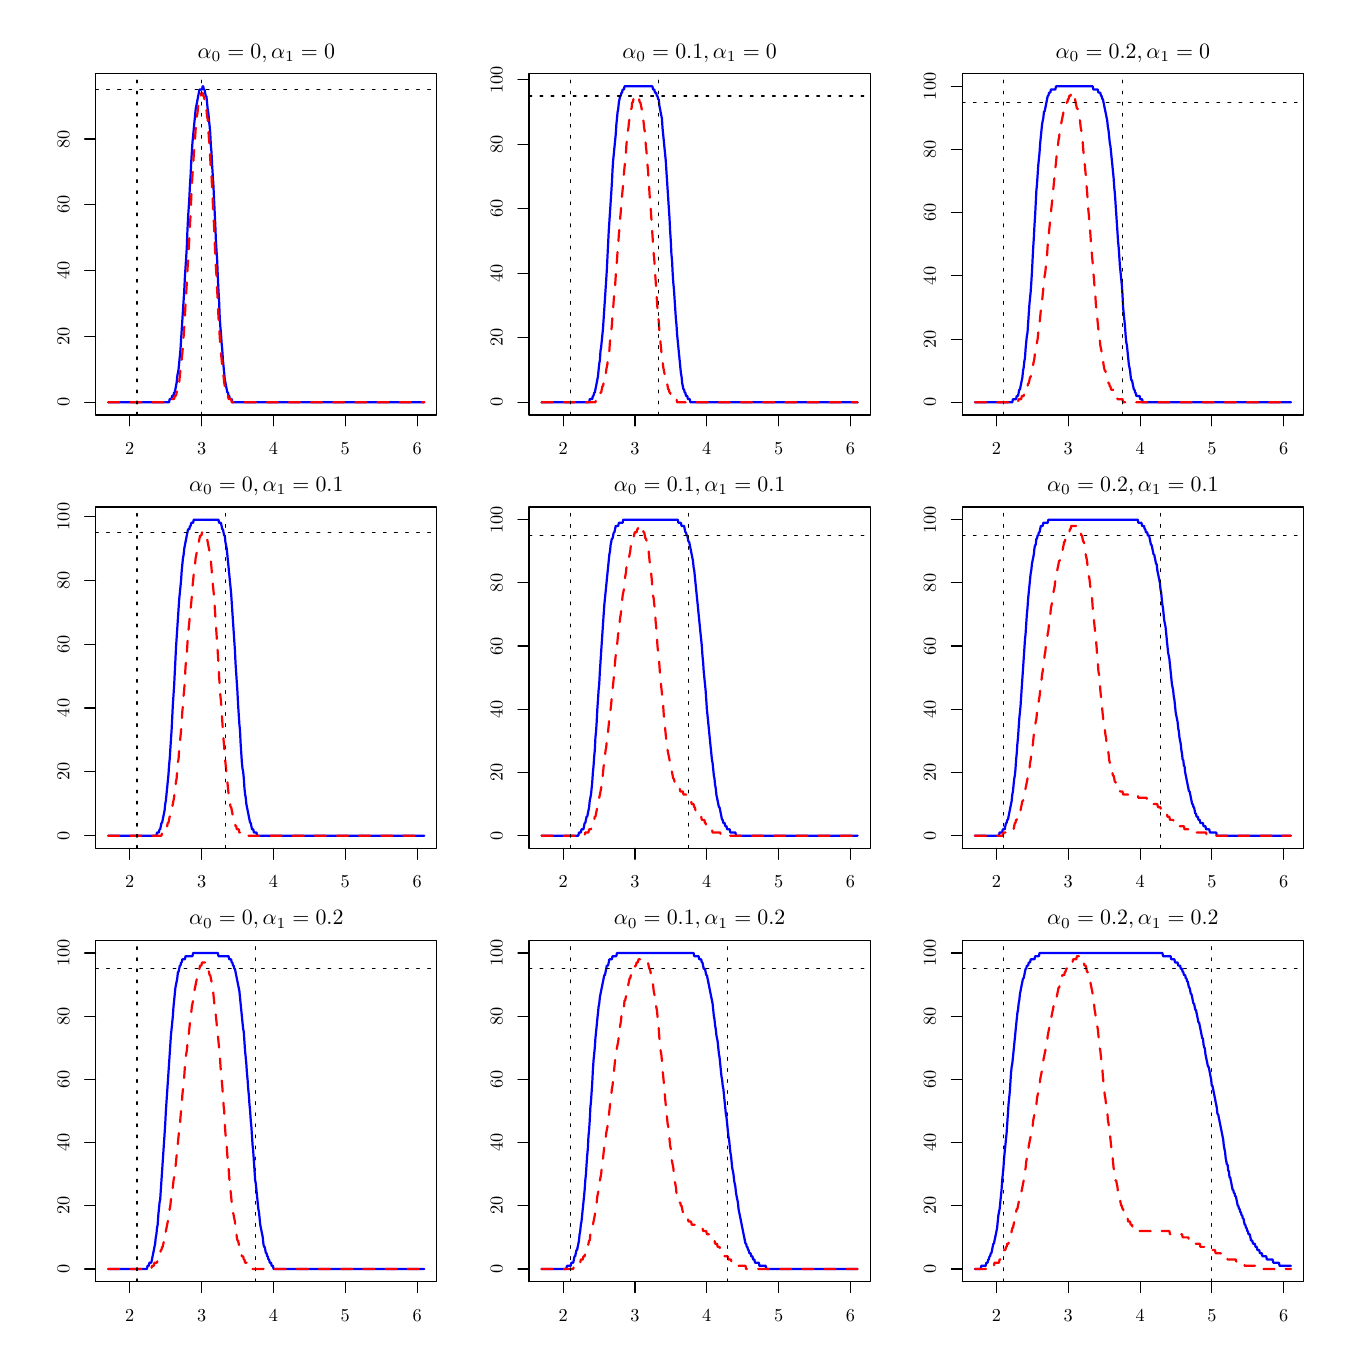
\begin{tikzpicture}[x=1pt,y=1pt]
\definecolor{fillColor}{RGB}{255,255,255}
\path[use as bounding box,fill=fillColor,fill opacity=0.00] (0,0) rectangle (469.75,469.75);
\begin{scope}
\path[clip] ( 24.55,329.80) rectangle (147.87,453.12);
\definecolor{drawColor}{RGB}{0,0,255}

\path[draw=drawColor,line width= 0.8pt,line join=round,line cap=round] ( 29.12,334.37) --
	( 29.35,334.37) --
	( 29.58,334.37) --
	( 29.81,334.37) --
	( 30.03,334.37) --
	( 30.26,334.37) --
	( 30.49,334.37) --
	( 30.72,334.37) --
	( 30.95,334.37) --
	( 31.18,334.37) --
	( 31.41,334.37) --
	( 31.64,334.37) --
	( 31.87,334.37) --
	( 32.09,334.37) --
	( 32.32,334.37) --
	( 32.55,334.37) --
	( 32.78,334.37) --
	( 33.01,334.37) --
	( 33.24,334.37) --
	( 33.47,334.37) --
	( 33.70,334.37) --
	( 33.92,334.37) --
	( 34.15,334.37) --
	( 34.38,334.37) --
	( 34.61,334.37) --
	( 34.84,334.37) --
	( 35.07,334.37) --
	( 35.30,334.37) --
	( 35.53,334.37) --
	( 35.76,334.37) --
	( 35.98,334.37) --
	( 36.21,334.37) --
	( 36.44,334.37) --
	( 36.67,334.37) --
	( 36.90,334.37) --
	( 37.13,334.37) --
	( 37.36,334.37) --
	( 37.59,334.37) --
	( 37.81,334.37) --
	( 38.04,334.37) --
	( 38.27,334.37) --
	( 38.50,334.37) --
	( 38.73,334.37) --
	( 38.96,334.37) --
	( 39.19,334.37) --
	( 39.42,334.37) --
	( 39.65,334.37) --
	( 39.87,334.37) --
	( 40.10,334.37) --
	( 40.33,334.37) --
	( 40.56,334.37) --
	( 40.79,334.37) --
	( 41.02,334.37) --
	( 41.25,334.37) --
	( 41.48,334.37) --
	( 41.71,334.37) --
	( 41.93,334.37) --
	( 42.16,334.37) --
	( 42.39,334.37) --
	( 42.62,334.37) --
	( 42.85,334.37) --
	( 43.08,334.37) --
	( 43.31,334.37) --
	( 43.54,334.37) --
	( 43.76,334.37) --
	( 43.99,334.37) --
	( 44.22,334.37) --
	( 44.45,334.37) --
	( 44.68,334.37) --
	( 44.91,334.37) --
	( 45.14,334.37) --
	( 45.37,334.37) --
	( 45.60,334.37) --
	( 45.82,334.37) --
	( 46.05,334.37) --
	( 46.28,334.37) --
	( 46.51,334.37) --
	( 46.74,334.37) --
	( 46.97,334.37) --
	( 47.20,334.37) --
	( 47.43,334.37) --
	( 47.65,334.37) --
	( 47.88,334.37) --
	( 48.11,334.37) --
	( 48.34,334.37) --
	( 48.57,334.37) --
	( 48.80,334.37) --
	( 49.03,334.37) --
	( 49.26,334.37) --
	( 49.49,334.37) --
	( 49.71,334.37) --
	( 49.94,334.37) --
	( 50.17,334.37) --
	( 50.40,334.37) --
	( 50.63,334.37) --
	( 50.86,334.37) --
	( 51.09,334.37) --
	( 51.32,335.56) --
	( 51.54,335.56) --
	( 51.77,335.56) --
	( 52.00,335.56) --
	( 52.23,336.75) --
	( 52.46,336.75) --
	( 52.69,336.75) --
	( 52.92,337.94) --
	( 53.15,337.94) --
	( 53.38,339.13) --
	( 53.60,340.32) --
	( 53.83,341.51) --
	( 54.06,343.88) --
	( 54.29,345.07) --
	( 54.52,346.26) --
	( 54.75,348.64) --
	( 54.98,351.02) --
	( 55.21,353.40) --
	( 55.43,356.97) --
	( 55.66,360.54) --
	( 55.89,364.11) --
	( 56.12,367.67) --
	( 56.35,371.24) --
	( 56.58,374.81) --
	( 56.81,379.57) --
	( 57.04,383.14) --
	( 57.27,386.70) --
	( 57.49,390.27) --
	( 57.72,396.22) --
	( 57.95,400.98) --
	( 58.18,404.55) --
	( 58.41,408.11) --
	( 58.64,412.87) --
	( 58.87,416.44) --
	( 59.10,421.20) --
	( 59.32,424.77) --
	( 59.55,428.34) --
	( 59.78,430.71) --
	( 60.01,433.09) --
	( 60.24,435.47) --
	( 60.47,437.85) --
	( 60.70,440.23) --
	( 60.93,441.42) --
	( 61.16,442.61) --
	( 61.38,443.80) --
	( 61.61,444.99) --
	( 61.84,446.18) --
	( 62.07,447.37) --
	( 62.30,447.37) --
	( 62.53,447.37) --
	( 62.76,447.37) --
	( 62.99,447.37) --
	( 63.22,448.56) --
	( 63.44,448.56) --
	( 63.67,447.37) --
	( 63.90,447.37) --
	( 64.13,446.18) --
	( 64.36,444.99) --
	( 64.59,444.99) --
	( 64.82,442.61) --
	( 65.05,440.23) --
	( 65.27,439.04) --
	( 65.50,436.66) --
	( 65.73,434.28) --
	( 65.96,431.90) --
	( 66.19,427.15) --
	( 66.42,424.77) --
	( 66.65,420.01) --
	( 66.88,416.44) --
	( 67.11,412.87) --
	( 67.33,408.11) --
	( 67.56,403.36) --
	( 67.79,398.60) --
	( 68.02,392.65) --
	( 68.25,389.08) --
	( 68.48,385.52) --
	( 68.71,379.57) --
	( 68.94,374.81) --
	( 69.16,371.24) --
	( 69.39,365.29) --
	( 69.62,361.73) --
	( 69.85,359.35) --
	( 70.08,355.78) --
	( 70.31,353.40) --
	( 70.54,349.83) --
	( 70.77,347.45) --
	( 71.00,345.07) --
	( 71.22,342.70) --
	( 71.45,341.51) --
	( 71.68,340.32) --
	( 71.91,339.13) --
	( 72.14,337.94) --
	( 72.37,337.94) --
	( 72.60,336.75) --
	( 72.83,336.75) --
	( 73.05,335.56) --
	( 73.28,335.56) --
	( 73.51,335.56) --
	( 73.74,335.56) --
	( 73.97,334.37) --
	( 74.20,334.37) --
	( 74.43,334.37) --
	( 74.66,334.37) --
	( 74.89,334.37) --
	( 75.11,334.37) --
	( 75.34,334.37) --
	( 75.57,334.37) --
	( 75.80,334.37) --
	( 76.03,334.37) --
	( 76.26,334.37) --
	( 76.49,334.37) --
	( 76.72,334.37) --
	( 76.94,334.37) --
	( 77.17,334.37) --
	( 77.40,334.37) --
	( 77.63,334.37) --
	( 77.86,334.37) --
	( 78.09,334.37) --
	( 78.32,334.37) --
	( 78.55,334.37) --
	( 78.78,334.37) --
	( 79.00,334.37) --
	( 79.23,334.37) --
	( 79.46,334.37) --
	( 79.69,334.37) --
	( 79.92,334.37) --
	( 80.15,334.37) --
	( 80.38,334.37) --
	( 80.61,334.37) --
	( 80.83,334.37) --
	( 81.06,334.37) --
	( 81.29,334.37) --
	( 81.52,334.37) --
	( 81.75,334.37) --
	( 81.98,334.37) --
	( 82.21,334.37) --
	( 82.44,334.37) --
	( 82.67,334.37) --
	( 82.89,334.37) --
	( 83.12,334.37) --
	( 83.35,334.37) --
	( 83.58,334.37) --
	( 83.81,334.37) --
	( 84.04,334.37) --
	( 84.27,334.37) --
	( 84.50,334.37) --
	( 84.73,334.37) --
	( 84.95,334.37) --
	( 85.18,334.37) --
	( 85.41,334.37) --
	( 85.64,334.37) --
	( 85.87,334.37) --
	( 86.10,334.37) --
	( 86.33,334.37) --
	( 86.56,334.37) --
	( 86.78,334.37) --
	( 87.01,334.37) --
	( 87.24,334.37) --
	( 87.47,334.37) --
	( 87.70,334.37) --
	( 87.93,334.37) --
	( 88.16,334.37) --
	( 88.39,334.37) --
	( 88.62,334.37) --
	( 88.84,334.37) --
	( 89.07,334.37) --
	( 89.30,334.37) --
	( 89.53,334.37) --
	( 89.76,334.37) --
	( 89.99,334.37) --
	( 90.22,334.37) --
	( 90.45,334.37) --
	( 90.67,334.37) --
	( 90.90,334.37) --
	( 91.13,334.37) --
	( 91.36,334.37) --
	( 91.59,334.37) --
	( 91.82,334.37) --
	( 92.05,334.37) --
	( 92.28,334.37) --
	( 92.51,334.37) --
	( 92.73,334.37) --
	( 92.96,334.37) --
	( 93.19,334.37) --
	( 93.42,334.37) --
	( 93.65,334.37) --
	( 93.88,334.37) --
	( 94.11,334.37) --
	( 94.34,334.37) --
	( 94.56,334.37) --
	( 94.79,334.37) --
	( 95.02,334.37) --
	( 95.25,334.37) --
	( 95.48,334.37) --
	( 95.71,334.37) --
	( 95.94,334.37) --
	( 96.17,334.37) --
	( 96.40,334.37) --
	( 96.62,334.37) --
	( 96.85,334.37) --
	( 97.08,334.37) --
	( 97.31,334.37) --
	( 97.54,334.37) --
	( 97.77,334.37) --
	( 98.00,334.37) --
	( 98.23,334.37) --
	( 98.45,334.37) --
	( 98.68,334.37) --
	( 98.91,334.37) --
	( 99.14,334.37) --
	( 99.37,334.37) --
	( 99.60,334.37) --
	( 99.83,334.37) --
	(100.06,334.37) --
	(100.29,334.37) --
	(100.51,334.37) --
	(100.74,334.37) --
	(100.97,334.37) --
	(101.20,334.37) --
	(101.43,334.37) --
	(101.66,334.37) --
	(101.89,334.37) --
	(102.12,334.37) --
	(102.35,334.37) --
	(102.57,334.37) --
	(102.80,334.37) --
	(103.03,334.37) --
	(103.26,334.37) --
	(103.49,334.37) --
	(103.72,334.37) --
	(103.95,334.37) --
	(104.18,334.37) --
	(104.40,334.37) --
	(104.63,334.37) --
	(104.86,334.37) --
	(105.09,334.37) --
	(105.32,334.37) --
	(105.55,334.37) --
	(105.78,334.37) --
	(106.01,334.37) --
	(106.24,334.37) --
	(106.46,334.37) --
	(106.69,334.37) --
	(106.92,334.37) --
	(107.15,334.37) --
	(107.38,334.37) --
	(107.61,334.37) --
	(107.84,334.37) --
	(108.07,334.37) --
	(108.29,334.37) --
	(108.52,334.37) --
	(108.75,334.37) --
	(108.98,334.37) --
	(109.21,334.37) --
	(109.44,334.37) --
	(109.67,334.37) --
	(109.90,334.37) --
	(110.13,334.37) --
	(110.35,334.37) --
	(110.58,334.37) --
	(110.81,334.37) --
	(111.04,334.37) --
	(111.27,334.37) --
	(111.50,334.37) --
	(111.73,334.37) --
	(111.96,334.37) --
	(112.18,334.37) --
	(112.41,334.37) --
	(112.64,334.37) --
	(112.87,334.37) --
	(113.10,334.37) --
	(113.33,334.37) --
	(113.56,334.37) --
	(113.79,334.37) --
	(114.02,334.37) --
	(114.24,334.37) --
	(114.47,334.37) --
	(114.70,334.37) --
	(114.93,334.37) --
	(115.16,334.37) --
	(115.39,334.37) --
	(115.62,334.37) --
	(115.85,334.37) --
	(116.07,334.37) --
	(116.30,334.37) --
	(116.53,334.37) --
	(116.76,334.37) --
	(116.99,334.37) --
	(117.22,334.37) --
	(117.45,334.37) --
	(117.68,334.37) --
	(117.91,334.37) --
	(118.13,334.37) --
	(118.36,334.37) --
	(118.59,334.37) --
	(118.82,334.37) --
	(119.05,334.37) --
	(119.28,334.37) --
	(119.51,334.37) --
	(119.74,334.37) --
	(119.96,334.37) --
	(120.19,334.37) --
	(120.42,334.37) --
	(120.65,334.37) --
	(120.88,334.37) --
	(121.11,334.37) --
	(121.34,334.37) --
	(121.57,334.37) --
	(121.80,334.37) --
	(122.02,334.37) --
	(122.25,334.37) --
	(122.48,334.37) --
	(122.71,334.37) --
	(122.94,334.37) --
	(123.17,334.37) --
	(123.40,334.37) --
	(123.63,334.37) --
	(123.86,334.37) --
	(124.08,334.37) --
	(124.31,334.37) --
	(124.54,334.37) --
	(124.77,334.37) --
	(125.00,334.37) --
	(125.23,334.37) --
	(125.46,334.37) --
	(125.69,334.37) --
	(125.91,334.37) --
	(126.14,334.37) --
	(126.37,334.37) --
	(126.60,334.37) --
	(126.83,334.37) --
	(127.06,334.37) --
	(127.29,334.37) --
	(127.52,334.37) --
	(127.75,334.37) --
	(127.97,334.37) --
	(128.20,334.37) --
	(128.43,334.37) --
	(128.66,334.37) --
	(128.89,334.37) --
	(129.12,334.37) --
	(129.35,334.37) --
	(129.58,334.37) --
	(129.80,334.37) --
	(130.03,334.37) --
	(130.26,334.37) --
	(130.49,334.37) --
	(130.72,334.37) --
	(130.95,334.37) --
	(131.18,334.37) --
	(131.41,334.37) --
	(131.64,334.37) --
	(131.86,334.37) --
	(132.09,334.37) --
	(132.32,334.37) --
	(132.55,334.37) --
	(132.78,334.37) --
	(133.01,334.37) --
	(133.24,334.37) --
	(133.47,334.37) --
	(133.69,334.37) --
	(133.92,334.37) --
	(134.15,334.37) --
	(134.38,334.37) --
	(134.61,334.37) --
	(134.84,334.37) --
	(135.07,334.37) --
	(135.30,334.37) --
	(135.53,334.37) --
	(135.75,334.37) --
	(135.98,334.37) --
	(136.21,334.37) --
	(136.44,334.37) --
	(136.67,334.37) --
	(136.90,334.37) --
	(137.13,334.37) --
	(137.36,334.37) --
	(137.58,334.37) --
	(137.81,334.37) --
	(138.04,334.37) --
	(138.27,334.37) --
	(138.50,334.37) --
	(138.73,334.37) --
	(138.96,334.37) --
	(139.19,334.37) --
	(139.42,334.37) --
	(139.64,334.37) --
	(139.87,334.37) --
	(140.10,334.37) --
	(140.33,334.37) --
	(140.56,334.37) --
	(140.79,334.37) --
	(141.02,334.37) --
	(141.25,334.37) --
	(141.47,334.37) --
	(141.70,334.37) --
	(141.93,334.37) --
	(142.16,334.37) --
	(142.39,334.37) --
	(142.62,334.37) --
	(142.85,334.37) --
	(143.08,334.37) --
	(143.31,334.37);
\end{scope}
\begin{scope}
\path[clip] (  0.00,  0.00) rectangle (469.75,469.75);
\definecolor{drawColor}{RGB}{0,0,0}

\path[draw=drawColor,line width= 0.4pt,line join=round,line cap=round] ( 36.90,329.80) -- (140.71,329.80);

\path[draw=drawColor,line width= 0.4pt,line join=round,line cap=round] ( 36.90,329.80) -- ( 36.90,325.84);

\path[draw=drawColor,line width= 0.4pt,line join=round,line cap=round] ( 62.86,329.80) -- ( 62.86,325.84);

\path[draw=drawColor,line width= 0.4pt,line join=round,line cap=round] ( 88.81,329.80) -- ( 88.81,325.84);

\path[draw=drawColor,line width= 0.4pt,line join=round,line cap=round] (114.76,329.80) -- (114.76,325.84);

\path[draw=drawColor,line width= 0.4pt,line join=round,line cap=round] (140.71,329.80) -- (140.71,325.84);

\node[text=drawColor,anchor=base,inner sep=0pt, outer sep=0pt, scale=  0.66] at ( 36.90,315.55) {2};

\node[text=drawColor,anchor=base,inner sep=0pt, outer sep=0pt, scale=  0.66] at ( 62.86,315.55) {3};

\node[text=drawColor,anchor=base,inner sep=0pt, outer sep=0pt, scale=  0.66] at ( 88.81,315.55) {4};

\node[text=drawColor,anchor=base,inner sep=0pt, outer sep=0pt, scale=  0.66] at (114.76,315.55) {5};

\node[text=drawColor,anchor=base,inner sep=0pt, outer sep=0pt, scale=  0.66] at (140.71,315.55) {6};

\path[draw=drawColor,line width= 0.4pt,line join=round,line cap=round] ( 24.55,334.37) -- ( 24.55,429.52);

\path[draw=drawColor,line width= 0.4pt,line join=round,line cap=round] ( 24.55,334.37) -- ( 20.59,334.37);

\path[draw=drawColor,line width= 0.4pt,line join=round,line cap=round] ( 24.55,358.16) -- ( 20.59,358.16);

\path[draw=drawColor,line width= 0.4pt,line join=round,line cap=round] ( 24.55,381.95) -- ( 20.59,381.95);

\path[draw=drawColor,line width= 0.4pt,line join=round,line cap=round] ( 24.55,405.74) -- ( 20.59,405.74);

\path[draw=drawColor,line width= 0.4pt,line join=round,line cap=round] ( 24.55,429.52) -- ( 20.59,429.52);

\node[text=drawColor,rotate= 90.00,anchor=base,inner sep=0pt, outer sep=0pt, scale=  0.66] at ( 15.05,334.37) {0};

\node[text=drawColor,rotate= 90.00,anchor=base,inner sep=0pt, outer sep=0pt, scale=  0.66] at ( 15.05,358.16) {20};

\node[text=drawColor,rotate= 90.00,anchor=base,inner sep=0pt, outer sep=0pt, scale=  0.66] at ( 15.05,381.95) {40};

\node[text=drawColor,rotate= 90.00,anchor=base,inner sep=0pt, outer sep=0pt, scale=  0.66] at ( 15.05,405.74) {60};

\node[text=drawColor,rotate= 90.00,anchor=base,inner sep=0pt, outer sep=0pt, scale=  0.66] at ( 15.05,429.52) {80};

\path[draw=drawColor,line width= 0.4pt,line join=round,line cap=round] ( 24.55,329.80) --
	(147.87,329.80) --
	(147.87,453.12) --
	( 24.55,453.12) --
	( 24.55,329.80);
\end{scope}
\begin{scope}
\path[clip] (  0.00,313.17) rectangle (156.58,469.75);
\definecolor{drawColor}{RGB}{0,0,0}

\node[text=drawColor,anchor=base,inner sep=0pt, outer sep=0pt, scale=  0.79] at ( 86.21,458.71) {\bfseries $\alpha_0 = 0, \alpha_1 = 0$};
\end{scope}
\begin{scope}
\path[clip] ( 24.55,329.80) rectangle (147.87,453.12);
\definecolor{drawColor}{RGB}{255,0,0}

\path[draw=drawColor,line width= 0.8pt,dash pattern=on 4pt off 4pt ,line join=round,line cap=round] ( 29.12,334.37) --
	( 29.35,334.37) --
	( 29.58,334.37) --
	( 29.81,334.37) --
	( 30.03,334.37) --
	( 30.26,334.37) --
	( 30.49,334.37) --
	( 30.72,334.37) --
	( 30.95,334.37) --
	( 31.18,334.37) --
	( 31.41,334.37) --
	( 31.64,334.37) --
	( 31.87,334.37) --
	( 32.09,334.37) --
	( 32.32,334.37) --
	( 32.55,334.37) --
	( 32.78,334.37) --
	( 33.01,334.37) --
	( 33.24,334.37) --
	( 33.47,334.37) --
	( 33.70,334.37) --
	( 33.92,334.37) --
	( 34.15,334.37) --
	( 34.38,334.37) --
	( 34.61,334.37) --
	( 34.84,334.37) --
	( 35.07,334.37) --
	( 35.30,334.37) --
	( 35.53,334.37) --
	( 35.76,334.37) --
	( 35.98,334.37) --
	( 36.21,334.37) --
	( 36.44,334.37) --
	( 36.67,334.37) --
	( 36.90,334.37) --
	( 37.13,334.37) --
	( 37.36,334.37) --
	( 37.59,334.37) --
	( 37.81,334.37) --
	( 38.04,334.37) --
	( 38.27,334.37) --
	( 38.50,334.37) --
	( 38.73,334.37) --
	( 38.96,334.37) --
	( 39.19,334.37) --
	( 39.42,334.37) --
	( 39.65,334.37) --
	( 39.87,334.37) --
	( 40.10,334.37) --
	( 40.33,334.37) --
	( 40.56,334.37) --
	( 40.79,334.37) --
	( 41.02,334.37) --
	( 41.25,334.37) --
	( 41.48,334.37) --
	( 41.71,334.37) --
	( 41.93,334.37) --
	( 42.16,334.37) --
	( 42.39,334.37) --
	( 42.62,334.37) --
	( 42.85,334.37) --
	( 43.08,334.37) --
	( 43.31,334.37) --
	( 43.54,334.37) --
	( 43.76,334.37) --
	( 43.99,334.37) --
	( 44.22,334.37) --
	( 44.45,334.37) --
	( 44.68,334.37) --
	( 44.91,334.37) --
	( 45.14,334.37) --
	( 45.37,334.37) --
	( 45.60,334.37) --
	( 45.82,334.37) --
	( 46.05,334.37) --
	( 46.28,334.37) --
	( 46.51,334.37) --
	( 46.74,334.37) --
	( 46.97,334.37) --
	( 47.20,334.37) --
	( 47.43,334.37) --
	( 47.65,334.37) --
	( 47.88,334.37) --
	( 48.11,334.37) --
	( 48.34,334.37) --
	( 48.57,334.37) --
	( 48.80,334.37) --
	( 49.03,334.37) --
	( 49.26,334.37) --
	( 49.49,334.37) --
	( 49.71,334.37) --
	( 49.94,334.37) --
	( 50.17,334.37) --
	( 50.40,334.37) --
	( 50.63,334.37) --
	( 50.86,334.37) --
	( 51.09,334.37) --
	( 51.32,334.37) --
	( 51.54,334.37) --
	( 51.77,334.37) --
	( 52.00,335.56) --
	( 52.23,335.56) --
	( 52.46,335.56) --
	( 52.69,335.56) --
	( 52.92,335.56) --
	( 53.15,336.75) --
	( 53.38,336.75) --
	( 53.60,336.75) --
	( 53.83,337.94) --
	( 54.06,339.13) --
	( 54.29,339.13) --
	( 54.52,341.51) --
	( 54.75,341.51) --
	( 54.98,343.88) --
	( 55.21,346.26) --
	( 55.43,347.45) --
	( 55.66,349.83) --
	( 55.89,352.21) --
	( 56.12,354.59) --
	( 56.35,358.16) --
	( 56.58,361.73) --
	( 56.81,365.29) --
	( 57.04,370.05) --
	( 57.27,373.62) --
	( 57.49,377.19) --
	( 57.72,381.95) --
	( 57.95,385.52) --
	( 58.18,389.08) --
	( 58.41,393.84) --
	( 58.64,398.60) --
	( 58.87,402.17) --
	( 59.10,408.11) --
	( 59.32,412.87) --
	( 59.55,416.44) --
	( 59.78,420.01) --
	( 60.01,423.58) --
	( 60.24,427.15) --
	( 60.47,429.52) --
	( 60.70,433.09) --
	( 60.93,435.47) --
	( 61.16,437.85) --
	( 61.38,439.04) --
	( 61.61,441.42) --
	( 61.84,442.61) --
	( 62.07,443.80) --
	( 62.30,444.99) --
	( 62.53,444.99) --
	( 62.76,446.18) --
	( 62.99,446.18) --
	( 63.22,446.18) --
	( 63.44,444.99) --
	( 63.67,444.99) --
	( 63.90,443.80) --
	( 64.13,442.61) --
	( 64.36,441.42) --
	( 64.59,440.23) --
	( 64.82,437.85) --
	( 65.05,436.66) --
	( 65.27,433.09) --
	( 65.50,429.52) --
	( 65.73,427.15) --
	( 65.96,422.39) --
	( 66.19,418.82) --
	( 66.42,416.44) --
	( 66.65,411.68) --
	( 66.88,406.93) --
	( 67.11,402.17) --
	( 67.33,398.60) --
	( 67.56,392.65) --
	( 67.79,387.89) --
	( 68.02,383.14) --
	( 68.25,379.57) --
	( 68.48,374.81) --
	( 68.71,370.05) --
	( 68.94,365.29) --
	( 69.16,361.73) --
	( 69.39,358.16) --
	( 69.62,354.59) --
	( 69.85,352.21) --
	( 70.08,349.83) --
	( 70.31,347.45) --
	( 70.54,345.07) --
	( 70.77,343.88) --
	( 71.00,341.51) --
	( 71.22,340.32) --
	( 71.45,339.13) --
	( 71.68,337.94) --
	( 71.91,337.94) --
	( 72.14,336.75) --
	( 72.37,336.75) --
	( 72.60,335.56) --
	( 72.83,335.56) --
	( 73.05,335.56) --
	( 73.28,335.56) --
	( 73.51,335.56) --
	( 73.74,334.37) --
	( 73.97,334.37) --
	( 74.20,334.37) --
	( 74.43,334.37) --
	( 74.66,334.37) --
	( 74.89,334.37) --
	( 75.11,334.37) --
	( 75.34,334.37) --
	( 75.57,334.37) --
	( 75.80,334.37) --
	( 76.03,334.37) --
	( 76.26,334.37) --
	( 76.49,334.37) --
	( 76.72,334.37) --
	( 76.94,334.37) --
	( 77.17,334.37) --
	( 77.40,334.37) --
	( 77.63,334.37) --
	( 77.86,334.37) --
	( 78.09,334.37) --
	( 78.32,334.37) --
	( 78.55,334.37) --
	( 78.78,334.37) --
	( 79.00,334.37) --
	( 79.23,334.37) --
	( 79.46,334.37) --
	( 79.69,334.37) --
	( 79.92,334.37) --
	( 80.15,334.37) --
	( 80.38,334.37) --
	( 80.61,334.37) --
	( 80.83,334.37) --
	( 81.06,334.37) --
	( 81.29,334.37) --
	( 81.52,334.37) --
	( 81.75,334.37) --
	( 81.98,334.37) --
	( 82.21,334.37) --
	( 82.44,334.37) --
	( 82.67,334.37) --
	( 82.89,334.37) --
	( 83.12,334.37) --
	( 83.35,334.37) --
	( 83.58,334.37) --
	( 83.81,334.37) --
	( 84.04,334.37) --
	( 84.27,334.37) --
	( 84.50,334.37) --
	( 84.73,334.37) --
	( 84.95,334.37) --
	( 85.18,334.37) --
	( 85.41,334.37) --
	( 85.64,334.37) --
	( 85.87,334.37) --
	( 86.10,334.37) --
	( 86.33,334.37) --
	( 86.56,334.37) --
	( 86.78,334.37) --
	( 87.01,334.37) --
	( 87.24,334.37) --
	( 87.47,334.37) --
	( 87.70,334.37) --
	( 87.93,334.37) --
	( 88.16,334.37) --
	( 88.39,334.37) --
	( 88.62,334.37) --
	( 88.84,334.37) --
	( 89.07,334.37) --
	( 89.30,334.37) --
	( 89.53,334.37) --
	( 89.76,334.37) --
	( 89.99,334.37) --
	( 90.22,334.37) --
	( 90.45,334.37) --
	( 90.67,334.37) --
	( 90.90,334.37) --
	( 91.13,334.37) --
	( 91.36,334.37) --
	( 91.59,334.37) --
	( 91.82,334.37) --
	( 92.05,334.37) --
	( 92.28,334.37) --
	( 92.51,334.37) --
	( 92.73,334.37) --
	( 92.96,334.37) --
	( 93.19,334.37) --
	( 93.42,334.37) --
	( 93.65,334.37) --
	( 93.88,334.37) --
	( 94.11,334.37) --
	( 94.34,334.37) --
	( 94.56,334.37) --
	( 94.79,334.37) --
	( 95.02,334.37) --
	( 95.25,334.37) --
	( 95.48,334.37) --
	( 95.71,334.37) --
	( 95.94,334.37) --
	( 96.17,334.37) --
	( 96.40,334.37) --
	( 96.62,334.37) --
	( 96.85,334.37) --
	( 97.08,334.37) --
	( 97.31,334.37) --
	( 97.54,334.37) --
	( 97.77,334.37) --
	( 98.00,334.37) --
	( 98.23,334.37) --
	( 98.45,334.37) --
	( 98.68,334.37) --
	( 98.91,334.37) --
	( 99.14,334.37) --
	( 99.37,334.37) --
	( 99.60,334.37) --
	( 99.83,334.37) --
	(100.06,334.37) --
	(100.29,334.37) --
	(100.51,334.37) --
	(100.74,334.37) --
	(100.97,334.37) --
	(101.20,334.37) --
	(101.43,334.37) --
	(101.66,334.37) --
	(101.89,334.37) --
	(102.12,334.37) --
	(102.35,334.37) --
	(102.57,334.37) --
	(102.80,334.37) --
	(103.03,334.37) --
	(103.26,334.37) --
	(103.49,334.37) --
	(103.72,334.37) --
	(103.95,334.37) --
	(104.18,334.37) --
	(104.40,334.37) --
	(104.63,334.37) --
	(104.86,334.37) --
	(105.09,334.37) --
	(105.32,334.37) --
	(105.55,334.37) --
	(105.78,334.37) --
	(106.01,334.37) --
	(106.24,334.37) --
	(106.46,334.37) --
	(106.69,334.37) --
	(106.92,334.37) --
	(107.15,334.37) --
	(107.38,334.37) --
	(107.61,334.37) --
	(107.84,334.37) --
	(108.07,334.37) --
	(108.29,334.37) --
	(108.52,334.37) --
	(108.75,334.37) --
	(108.98,334.37) --
	(109.21,334.37) --
	(109.44,334.37) --
	(109.67,334.37) --
	(109.90,334.37) --
	(110.13,334.37) --
	(110.35,334.37) --
	(110.58,334.37) --
	(110.81,334.37) --
	(111.04,334.37) --
	(111.27,334.37) --
	(111.50,334.37) --
	(111.73,334.37) --
	(111.96,334.37) --
	(112.18,334.37) --
	(112.41,334.37) --
	(112.64,334.37) --
	(112.87,334.37) --
	(113.10,334.37) --
	(113.33,334.37) --
	(113.56,334.37) --
	(113.79,334.37) --
	(114.02,334.37) --
	(114.24,334.37) --
	(114.47,334.37) --
	(114.70,334.37) --
	(114.93,334.37) --
	(115.16,334.37) --
	(115.39,334.37) --
	(115.62,334.37) --
	(115.85,334.37) --
	(116.07,334.37) --
	(116.30,334.37) --
	(116.53,334.37) --
	(116.76,334.37) --
	(116.99,334.37) --
	(117.22,334.37) --
	(117.45,334.37) --
	(117.68,334.37) --
	(117.91,334.37) --
	(118.13,334.37) --
	(118.36,334.37) --
	(118.59,334.37) --
	(118.82,334.37) --
	(119.05,334.37) --
	(119.28,334.37) --
	(119.51,334.37) --
	(119.74,334.37) --
	(119.96,334.37) --
	(120.19,334.37) --
	(120.42,334.37) --
	(120.65,334.37) --
	(120.88,334.37) --
	(121.11,334.37) --
	(121.34,334.37) --
	(121.57,334.37) --
	(121.80,334.37) --
	(122.02,334.37) --
	(122.25,334.37) --
	(122.48,334.37) --
	(122.71,334.37) --
	(122.94,334.37) --
	(123.17,334.37) --
	(123.40,334.37) --
	(123.63,334.37) --
	(123.86,334.37) --
	(124.08,334.37) --
	(124.31,334.37) --
	(124.54,334.37) --
	(124.77,334.37) --
	(125.00,334.37) --
	(125.23,334.37) --
	(125.46,334.37) --
	(125.69,334.37) --
	(125.91,334.37) --
	(126.14,334.37) --
	(126.37,334.37) --
	(126.60,334.37) --
	(126.83,334.37) --
	(127.06,334.37) --
	(127.29,334.37) --
	(127.52,334.37) --
	(127.75,334.37) --
	(127.97,334.37) --
	(128.20,334.37) --
	(128.43,334.37) --
	(128.66,334.37) --
	(128.89,334.37) --
	(129.12,334.37) --
	(129.35,334.37) --
	(129.58,334.37) --
	(129.80,334.37) --
	(130.03,334.37) --
	(130.26,334.37) --
	(130.49,334.37) --
	(130.72,334.37) --
	(130.95,334.37) --
	(131.18,334.37) --
	(131.41,334.37) --
	(131.64,334.37) --
	(131.86,334.37) --
	(132.09,334.37) --
	(132.32,334.37) --
	(132.55,334.37) --
	(132.78,334.37) --
	(133.01,334.37) --
	(133.24,334.37) --
	(133.47,334.37) --
	(133.69,334.37) --
	(133.92,334.37) --
	(134.15,334.37) --
	(134.38,334.37) --
	(134.61,334.37) --
	(134.84,334.37) --
	(135.07,334.37) --
	(135.30,334.37) --
	(135.53,334.37) --
	(135.75,334.37) --
	(135.98,334.37) --
	(136.21,334.37) --
	(136.44,334.37) --
	(136.67,334.37) --
	(136.90,334.37) --
	(137.13,334.37) --
	(137.36,334.37) --
	(137.58,334.37) --
	(137.81,334.37) --
	(138.04,334.37) --
	(138.27,334.37) --
	(138.50,334.37) --
	(138.73,334.37) --
	(138.96,334.37) --
	(139.19,334.37) --
	(139.42,334.37) --
	(139.64,334.37) --
	(139.87,334.37) --
	(140.10,334.37) --
	(140.33,334.37) --
	(140.56,334.37) --
	(140.79,334.37) --
	(141.02,334.37) --
	(141.25,334.37) --
	(141.47,334.37) --
	(141.70,334.37) --
	(141.93,334.37) --
	(142.16,334.37) --
	(142.39,334.37) --
	(142.62,334.37) --
	(142.85,334.37) --
	(143.08,334.37) --
	(143.31,334.37);
\definecolor{drawColor}{RGB}{0,0,0}

\path[draw=drawColor,line width= 0.4pt,dash pattern=on 1pt off 3pt ,line join=round,line cap=round] ( 24.55,447.37) -- (147.87,447.37);

\path[draw=drawColor,line width= 0.4pt,dash pattern=on 1pt off 3pt ,line join=round,line cap=round] ( 39.50,329.80) -- ( 39.50,453.12);

\path[draw=drawColor,line width= 0.4pt,dash pattern=on 1pt off 3pt ,line join=round,line cap=round] ( 62.86,329.80) -- ( 62.86,453.12);
\end{scope}
\begin{scope}
\path[clip] (181.14,329.80) rectangle (304.46,453.12);
\definecolor{drawColor}{RGB}{0,0,255}

\path[draw=drawColor,line width= 0.8pt,line join=round,line cap=round] (185.70,334.37) --
	(185.93,334.37) --
	(186.16,334.37) --
	(186.39,334.37) --
	(186.62,334.37) --
	(186.85,334.37) --
	(187.08,334.37) --
	(187.31,334.37) --
	(187.54,334.37) --
	(187.76,334.37) --
	(187.99,334.37) --
	(188.22,334.37) --
	(188.45,334.37) --
	(188.68,334.37) --
	(188.91,334.37) --
	(189.14,334.37) --
	(189.37,334.37) --
	(189.59,334.37) --
	(189.82,334.37) --
	(190.05,334.37) --
	(190.28,334.37) --
	(190.51,334.37) --
	(190.74,334.37) --
	(190.97,334.37) --
	(191.20,334.37) --
	(191.43,334.37) --
	(191.65,334.37) --
	(191.88,334.37) --
	(192.11,334.37) --
	(192.34,334.37) --
	(192.57,334.37) --
	(192.80,334.37) --
	(193.03,334.37) --
	(193.26,334.37) --
	(193.48,334.37) --
	(193.71,334.37) --
	(193.94,334.37) --
	(194.17,334.37) --
	(194.40,334.37) --
	(194.63,334.37) --
	(194.86,334.37) --
	(195.09,334.37) --
	(195.32,334.37) --
	(195.54,334.37) --
	(195.77,334.37) --
	(196.00,334.37) --
	(196.23,334.37) --
	(196.46,334.37) --
	(196.69,334.37) --
	(196.92,334.37) --
	(197.15,334.37) --
	(197.37,334.37) --
	(197.60,334.37) --
	(197.83,334.37) --
	(198.06,334.37) --
	(198.29,334.37) --
	(198.52,334.37) --
	(198.75,334.37) --
	(198.98,334.37) --
	(199.21,334.37) --
	(199.43,334.37) --
	(199.66,334.37) --
	(199.89,334.37) --
	(200.12,334.37) --
	(200.35,334.37) --
	(200.58,334.37) --
	(200.81,334.37) --
	(201.04,334.37) --
	(201.26,334.37) --
	(201.49,334.37) --
	(201.72,334.37) --
	(201.95,334.37) --
	(202.18,334.37) --
	(202.41,334.37) --
	(202.64,334.37) --
	(202.87,334.37) --
	(203.10,335.53) --
	(203.32,335.53) --
	(203.55,335.53) --
	(203.78,335.53) --
	(204.01,335.53) --
	(204.24,336.70) --
	(204.47,336.70) --
	(204.70,337.86) --
	(204.93,337.86) --
	(205.15,339.03) --
	(205.38,340.20) --
	(205.61,341.36) --
	(205.84,342.53) --
	(206.07,343.69) --
	(206.30,346.02) --
	(206.53,348.35) --
	(206.76,349.52) --
	(206.99,353.01) --
	(207.21,354.18) --
	(207.44,356.51) --
	(207.67,358.84) --
	(207.90,361.17) --
	(208.13,364.66) --
	(208.36,368.16) --
	(208.59,371.65) --
	(208.82,375.15) --
	(209.05,378.65) --
	(209.27,382.14) --
	(209.50,386.80) --
	(209.73,391.46) --
	(209.96,396.12) --
	(210.19,399.62) --
	(210.42,403.11) --
	(210.65,406.61) --
	(210.88,410.11) --
	(211.10,413.60) --
	(211.33,418.26) --
	(211.56,421.76) --
	(211.79,424.09) --
	(212.02,426.42) --
	(212.25,428.75) --
	(212.48,431.08) --
	(212.71,434.57) --
	(212.94,436.90) --
	(213.16,439.23) --
	(213.39,440.40) --
	(213.62,442.73) --
	(213.85,443.89) --
	(214.08,445.06) --
	(214.31,445.06) --
	(214.54,446.23) --
	(214.77,446.23) --
	(214.99,447.39) --
	(215.22,447.39) --
	(215.45,447.39) --
	(215.68,448.56) --
	(215.91,448.56) --
	(216.14,448.56) --
	(216.37,448.56) --
	(216.60,448.56) --
	(216.83,448.56) --
	(217.05,448.56) --
	(217.28,448.56) --
	(217.51,448.56) --
	(217.74,448.56) --
	(217.97,448.56) --
	(218.20,448.56) --
	(218.43,448.56) --
	(218.66,448.56) --
	(218.88,448.56) --
	(219.11,448.56) --
	(219.34,448.56) --
	(219.57,448.56) --
	(219.80,448.56) --
	(220.03,448.56) --
	(220.26,448.56) --
	(220.49,448.56) --
	(220.72,448.56) --
	(220.94,448.56) --
	(221.17,448.56) --
	(221.40,448.56) --
	(221.63,448.56) --
	(221.86,448.56) --
	(222.09,448.56) --
	(222.32,448.56) --
	(222.55,448.56) --
	(222.77,448.56) --
	(223.00,448.56) --
	(223.23,448.56) --
	(223.46,448.56) --
	(223.69,448.56) --
	(223.92,448.56) --
	(224.15,448.56) --
	(224.38,448.56) --
	(224.61,448.56) --
	(224.83,448.56) --
	(225.06,448.56) --
	(225.29,448.56) --
	(225.52,448.56) --
	(225.75,448.56) --
	(225.98,447.39) --
	(226.21,447.39) --
	(226.44,447.39) --
	(226.66,446.23) --
	(226.89,446.23) --
	(227.12,446.23) --
	(227.35,445.06) --
	(227.58,445.06) --
	(227.81,443.89) --
	(228.04,443.89) --
	(228.27,441.56) --
	(228.50,440.40) --
	(228.72,439.23) --
	(228.95,438.07) --
	(229.18,436.90) --
	(229.41,433.41) --
	(229.64,431.08) --
	(229.87,428.75) --
	(230.10,426.42) --
	(230.33,424.09) --
	(230.56,421.76) --
	(230.78,418.26) --
	(231.01,414.77) --
	(231.24,411.27) --
	(231.47,407.77) --
	(231.70,404.28) --
	(231.93,400.78) --
	(232.16,396.12) --
	(232.39,392.63) --
	(232.61,387.97) --
	(232.84,385.64) --
	(233.07,380.98) --
	(233.30,377.48) --
	(233.53,375.15) --
	(233.76,371.65) --
	(233.99,368.16) --
	(234.22,364.66) --
	(234.45,362.33) --
	(234.67,358.84) --
	(234.90,356.51) --
	(235.13,354.18) --
	(235.36,351.85) --
	(235.59,349.52) --
	(235.82,347.19) --
	(236.05,344.86) --
	(236.28,343.69) --
	(236.50,341.36) --
	(236.73,340.20) --
	(236.96,339.03) --
	(237.19,339.03) --
	(237.42,337.86) --
	(237.65,337.86) --
	(237.88,336.70) --
	(238.11,336.70) --
	(238.34,336.70) --
	(238.56,335.53) --
	(238.79,335.53) --
	(239.02,335.53) --
	(239.25,335.53) --
	(239.48,334.37) --
	(239.71,334.37) --
	(239.94,334.37) --
	(240.17,334.37) --
	(240.39,334.37) --
	(240.62,334.37) --
	(240.85,334.37) --
	(241.08,334.37) --
	(241.31,334.37) --
	(241.54,334.37) --
	(241.77,334.37) --
	(242.00,334.37) --
	(242.23,334.37) --
	(242.45,334.37) --
	(242.68,334.37) --
	(242.91,334.37) --
	(243.14,334.37) --
	(243.37,334.37) --
	(243.60,334.37) --
	(243.83,334.37) --
	(244.06,334.37) --
	(244.28,334.37) --
	(244.51,334.37) --
	(244.74,334.37) --
	(244.97,334.37) --
	(245.20,334.37) --
	(245.43,334.37) --
	(245.66,334.37) --
	(245.89,334.37) --
	(246.12,334.37) --
	(246.34,334.37) --
	(246.57,334.37) --
	(246.80,334.37) --
	(247.03,334.37) --
	(247.26,334.37) --
	(247.49,334.37) --
	(247.72,334.37) --
	(247.95,334.37) --
	(248.18,334.37) --
	(248.40,334.37) --
	(248.63,334.37) --
	(248.86,334.37) --
	(249.09,334.37) --
	(249.32,334.37) --
	(249.55,334.37) --
	(249.78,334.37) --
	(250.01,334.37) --
	(250.23,334.37) --
	(250.46,334.37) --
	(250.69,334.37) --
	(250.92,334.37) --
	(251.15,334.37) --
	(251.38,334.37) --
	(251.61,334.37) --
	(251.84,334.37) --
	(252.07,334.37) --
	(252.29,334.37) --
	(252.52,334.37) --
	(252.75,334.37) --
	(252.98,334.37) --
	(253.21,334.37) --
	(253.44,334.37) --
	(253.67,334.37) --
	(253.90,334.37) --
	(254.12,334.37) --
	(254.35,334.37) --
	(254.58,334.37) --
	(254.81,334.37) --
	(255.04,334.37) --
	(255.27,334.37) --
	(255.50,334.37) --
	(255.73,334.37) --
	(255.96,334.37) --
	(256.18,334.37) --
	(256.41,334.37) --
	(256.64,334.37) --
	(256.87,334.37) --
	(257.10,334.37) --
	(257.33,334.37) --
	(257.56,334.37) --
	(257.79,334.37) --
	(258.01,334.37) --
	(258.24,334.37) --
	(258.47,334.37) --
	(258.70,334.37) --
	(258.93,334.37) --
	(259.16,334.37) --
	(259.39,334.37) --
	(259.62,334.37) --
	(259.85,334.37) --
	(260.07,334.37) --
	(260.30,334.37) --
	(260.53,334.37) --
	(260.76,334.37) --
	(260.99,334.37) --
	(261.22,334.37) --
	(261.45,334.37) --
	(261.68,334.37) --
	(261.90,334.37) --
	(262.13,334.37) --
	(262.36,334.37) --
	(262.59,334.37) --
	(262.82,334.37) --
	(263.05,334.37) --
	(263.28,334.37) --
	(263.51,334.37) --
	(263.74,334.37) --
	(263.96,334.37) --
	(264.19,334.37) --
	(264.42,334.37) --
	(264.65,334.37) --
	(264.88,334.37) --
	(265.11,334.37) --
	(265.34,334.37) --
	(265.57,334.37) --
	(265.79,334.37) --
	(266.02,334.37) --
	(266.25,334.37) --
	(266.48,334.37) --
	(266.71,334.37) --
	(266.94,334.37) --
	(267.17,334.37) --
	(267.40,334.37) --
	(267.63,334.37) --
	(267.85,334.37) --
	(268.08,334.37) --
	(268.31,334.37) --
	(268.54,334.37) --
	(268.77,334.37) --
	(269.00,334.37) --
	(269.23,334.37) --
	(269.46,334.37) --
	(269.69,334.37) --
	(269.91,334.37) --
	(270.14,334.37) --
	(270.37,334.37) --
	(270.60,334.37) --
	(270.83,334.37) --
	(271.06,334.37) --
	(271.29,334.37) --
	(271.52,334.37) --
	(271.74,334.37) --
	(271.97,334.37) --
	(272.20,334.37) --
	(272.43,334.37) --
	(272.66,334.37) --
	(272.89,334.37) --
	(273.12,334.37) --
	(273.35,334.37) --
	(273.58,334.37) --
	(273.80,334.37) --
	(274.03,334.37) --
	(274.26,334.37) --
	(274.49,334.37) --
	(274.72,334.37) --
	(274.95,334.37) --
	(275.18,334.37) --
	(275.41,334.37) --
	(275.63,334.37) --
	(275.86,334.37) --
	(276.09,334.37) --
	(276.32,334.37) --
	(276.55,334.37) --
	(276.78,334.37) --
	(277.01,334.37) --
	(277.24,334.37) --
	(277.47,334.37) --
	(277.69,334.37) --
	(277.92,334.37) --
	(278.15,334.37) --
	(278.38,334.37) --
	(278.61,334.37) --
	(278.84,334.37) --
	(279.07,334.37) --
	(279.30,334.37) --
	(279.52,334.37) --
	(279.75,334.37) --
	(279.98,334.37) --
	(280.21,334.37) --
	(280.44,334.37) --
	(280.67,334.37) --
	(280.90,334.37) --
	(281.13,334.37) --
	(281.36,334.37) --
	(281.58,334.37) --
	(281.81,334.37) --
	(282.04,334.37) --
	(282.27,334.37) --
	(282.50,334.37) --
	(282.73,334.37) --
	(282.96,334.37) --
	(283.19,334.37) --
	(283.41,334.37) --
	(283.64,334.37) --
	(283.87,334.37) --
	(284.10,334.37) --
	(284.33,334.37) --
	(284.56,334.37) --
	(284.79,334.37) --
	(285.02,334.37) --
	(285.25,334.37) --
	(285.47,334.37) --
	(285.70,334.37) --
	(285.93,334.37) --
	(286.16,334.37) --
	(286.39,334.37) --
	(286.62,334.37) --
	(286.85,334.37) --
	(287.08,334.37) --
	(287.30,334.37) --
	(287.53,334.37) --
	(287.76,334.37) --
	(287.99,334.37) --
	(288.22,334.37) --
	(288.45,334.37) --
	(288.68,334.37) --
	(288.91,334.37) --
	(289.14,334.37) --
	(289.36,334.37) --
	(289.59,334.37) --
	(289.82,334.37) --
	(290.05,334.37) --
	(290.28,334.37) --
	(290.51,334.37) --
	(290.74,334.37) --
	(290.97,334.37) --
	(291.20,334.37) --
	(291.42,334.37) --
	(291.65,334.37) --
	(291.88,334.37) --
	(292.11,334.37) --
	(292.34,334.37) --
	(292.57,334.37) --
	(292.80,334.37) --
	(293.03,334.37) --
	(293.25,334.37) --
	(293.48,334.37) --
	(293.71,334.37) --
	(293.94,334.37) --
	(294.17,334.37) --
	(294.40,334.37) --
	(294.63,334.37) --
	(294.86,334.37) --
	(295.09,334.37) --
	(295.31,334.37) --
	(295.54,334.37) --
	(295.77,334.37) --
	(296.00,334.37) --
	(296.23,334.37) --
	(296.46,334.37) --
	(296.69,334.37) --
	(296.92,334.37) --
	(297.14,334.37) --
	(297.37,334.37) --
	(297.60,334.37) --
	(297.83,334.37) --
	(298.06,334.37) --
	(298.29,334.37) --
	(298.52,334.37) --
	(298.75,334.37) --
	(298.98,334.37) --
	(299.20,334.37) --
	(299.43,334.37) --
	(299.66,334.37) --
	(299.89,334.37);
\end{scope}
\begin{scope}
\path[clip] (  0.00,  0.00) rectangle (469.75,469.75);
\definecolor{drawColor}{RGB}{0,0,0}

\path[draw=drawColor,line width= 0.4pt,line join=round,line cap=round] (193.49,329.80) -- (297.30,329.80);

\path[draw=drawColor,line width= 0.4pt,line join=round,line cap=round] (193.49,329.80) -- (193.49,325.84);

\path[draw=drawColor,line width= 0.4pt,line join=round,line cap=round] (219.44,329.80) -- (219.44,325.84);

\path[draw=drawColor,line width= 0.4pt,line join=round,line cap=round] (245.39,329.80) -- (245.39,325.84);

\path[draw=drawColor,line width= 0.4pt,line join=round,line cap=round] (271.34,329.80) -- (271.34,325.84);

\path[draw=drawColor,line width= 0.4pt,line join=round,line cap=round] (297.30,329.80) -- (297.30,325.84);

\node[text=drawColor,anchor=base,inner sep=0pt, outer sep=0pt, scale=  0.66] at (193.49,315.55) {2};

\node[text=drawColor,anchor=base,inner sep=0pt, outer sep=0pt, scale=  0.66] at (219.44,315.55) {3};

\node[text=drawColor,anchor=base,inner sep=0pt, outer sep=0pt, scale=  0.66] at (245.39,315.55) {4};

\node[text=drawColor,anchor=base,inner sep=0pt, outer sep=0pt, scale=  0.66] at (271.34,315.55) {5};

\node[text=drawColor,anchor=base,inner sep=0pt, outer sep=0pt, scale=  0.66] at (297.30,315.55) {6};

\path[draw=drawColor,line width= 0.4pt,line join=round,line cap=round] (181.14,334.37) -- (181.14,450.89);

\path[draw=drawColor,line width= 0.4pt,line join=round,line cap=round] (181.14,334.37) -- (177.18,334.37);

\path[draw=drawColor,line width= 0.4pt,line join=round,line cap=round] (181.14,357.67) -- (177.18,357.67);

\path[draw=drawColor,line width= 0.4pt,line join=round,line cap=round] (181.14,380.98) -- (177.18,380.98);

\path[draw=drawColor,line width= 0.4pt,line join=round,line cap=round] (181.14,404.28) -- (177.18,404.28);

\path[draw=drawColor,line width= 0.4pt,line join=round,line cap=round] (181.14,427.58) -- (177.18,427.58);

\path[draw=drawColor,line width= 0.4pt,line join=round,line cap=round] (181.14,450.89) -- (177.18,450.89);

\node[text=drawColor,rotate= 90.00,anchor=base,inner sep=0pt, outer sep=0pt, scale=  0.66] at (171.63,334.37) {0};

\node[text=drawColor,rotate= 90.00,anchor=base,inner sep=0pt, outer sep=0pt, scale=  0.66] at (171.63,357.67) {20};

\node[text=drawColor,rotate= 90.00,anchor=base,inner sep=0pt, outer sep=0pt, scale=  0.66] at (171.63,380.98) {40};

\node[text=drawColor,rotate= 90.00,anchor=base,inner sep=0pt, outer sep=0pt, scale=  0.66] at (171.63,404.28) {60};

\node[text=drawColor,rotate= 90.00,anchor=base,inner sep=0pt, outer sep=0pt, scale=  0.66] at (171.63,427.58) {80};

\node[text=drawColor,rotate= 90.00,anchor=base,inner sep=0pt, outer sep=0pt, scale=  0.66] at (171.63,450.89) {100};

\path[draw=drawColor,line width= 0.4pt,line join=round,line cap=round] (181.14,329.80) --
	(304.46,329.80) --
	(304.46,453.12) --
	(181.14,453.12) --
	(181.14,329.80);
\end{scope}
\begin{scope}
\path[clip] (156.58,313.17) rectangle (313.17,469.75);
\definecolor{drawColor}{RGB}{0,0,0}

\node[text=drawColor,anchor=base,inner sep=0pt, outer sep=0pt, scale=  0.79] at (242.80,458.71) {\bfseries $\alpha_0 = 0.1, \alpha_1 = 0$};
\end{scope}
\begin{scope}
\path[clip] (181.14,329.80) rectangle (304.46,453.12);
\definecolor{drawColor}{RGB}{255,0,0}

\path[draw=drawColor,line width= 0.8pt,dash pattern=on 4pt off 4pt ,line join=round,line cap=round] (185.70,334.37) --
	(185.93,334.37) --
	(186.16,334.37) --
	(186.39,334.37) --
	(186.62,334.37) --
	(186.85,334.37) --
	(187.08,334.37) --
	(187.31,334.37) --
	(187.54,334.37) --
	(187.76,334.37) --
	(187.99,334.37) --
	(188.22,334.37) --
	(188.45,334.37) --
	(188.68,334.37) --
	(188.91,334.37) --
	(189.14,334.37) --
	(189.37,334.37) --
	(189.59,334.37) --
	(189.82,334.37) --
	(190.05,334.37) --
	(190.28,334.37) --
	(190.51,334.37) --
	(190.74,334.37) --
	(190.97,334.37) --
	(191.20,334.37) --
	(191.43,334.37) --
	(191.65,334.37) --
	(191.88,334.37) --
	(192.11,334.37) --
	(192.34,334.37) --
	(192.57,334.37) --
	(192.80,334.37) --
	(193.03,334.37) --
	(193.26,334.37) --
	(193.48,334.37) --
	(193.71,334.37) --
	(193.94,334.37) --
	(194.17,334.37) --
	(194.40,334.37) --
	(194.63,334.37) --
	(194.86,334.37) --
	(195.09,334.37) --
	(195.32,334.37) --
	(195.54,334.37) --
	(195.77,334.37) --
	(196.00,334.37) --
	(196.23,334.37) --
	(196.46,334.37) --
	(196.69,334.37) --
	(196.92,334.37) --
	(197.15,334.37) --
	(197.37,334.37) --
	(197.60,334.37) --
	(197.83,334.37) --
	(198.06,334.37) --
	(198.29,334.37) --
	(198.52,334.37) --
	(198.75,334.37) --
	(198.98,334.37) --
	(199.21,334.37) --
	(199.43,334.37) --
	(199.66,334.37) --
	(199.89,334.37) --
	(200.12,334.37) --
	(200.35,334.37) --
	(200.58,334.37) --
	(200.81,334.37) --
	(201.04,334.37) --
	(201.26,334.37) --
	(201.49,334.37) --
	(201.72,334.37) --
	(201.95,334.37) --
	(202.18,334.37) --
	(202.41,334.37) --
	(202.64,334.37) --
	(202.87,334.37) --
	(203.10,334.37) --
	(203.32,334.37) --
	(203.55,334.37) --
	(203.78,334.37) --
	(204.01,334.37) --
	(204.24,334.37) --
	(204.47,334.37) --
	(204.70,334.37) --
	(204.93,334.37) --
	(205.15,334.37) --
	(205.38,335.53) --
	(205.61,335.53) --
	(205.84,335.53) --
	(206.07,335.53) --
	(206.30,335.53) --
	(206.53,336.70) --
	(206.76,336.70) --
	(206.99,337.86) --
	(207.21,337.86) --
	(207.44,339.03) --
	(207.67,340.20) --
	(207.90,340.20) --
	(208.13,341.36) --
	(208.36,341.36) --
	(208.59,342.53) --
	(208.82,343.69) --
	(209.05,346.02) --
	(209.27,347.19) --
	(209.50,348.35) --
	(209.73,350.68) --
	(209.96,351.85) --
	(210.19,353.01) --
	(210.42,356.51) --
	(210.65,358.84) --
	(210.88,360.00) --
	(211.10,362.33) --
	(211.33,365.83) --
	(211.56,368.16) --
	(211.79,371.65) --
	(212.02,373.99) --
	(212.25,376.32) --
	(212.48,379.81) --
	(212.71,383.31) --
	(212.94,385.64) --
	(213.16,389.13) --
	(213.39,391.46) --
	(213.62,394.96) --
	(213.85,397.29) --
	(214.08,400.78) --
	(214.31,403.11) --
	(214.54,406.61) --
	(214.77,408.94) --
	(214.99,411.27) --
	(215.22,413.60) --
	(215.45,417.10) --
	(215.68,419.43) --
	(215.91,421.76) --
	(216.14,424.09) --
	(216.37,427.58) --
	(216.60,429.91) --
	(216.83,432.24) --
	(217.05,433.41) --
	(217.28,435.74) --
	(217.51,436.90) --
	(217.74,438.07) --
	(217.97,440.40) --
	(218.20,440.40) --
	(218.43,442.73) --
	(218.66,442.73) --
	(218.88,443.89) --
	(219.11,443.89) --
	(219.34,445.06) --
	(219.57,445.06) --
	(219.80,445.06) --
	(220.03,445.06) --
	(220.26,445.06) --
	(220.49,445.06) --
	(220.72,445.06) --
	(220.94,443.89) --
	(221.17,442.73) --
	(221.40,442.73) --
	(221.63,441.56) --
	(221.86,440.40) --
	(222.09,439.23) --
	(222.32,436.90) --
	(222.55,435.74) --
	(222.77,433.41) --
	(223.00,432.24) --
	(223.23,428.75) --
	(223.46,426.42) --
	(223.69,424.09) --
	(223.92,420.59) --
	(224.15,418.26) --
	(224.38,414.77) --
	(224.61,411.27) --
	(224.83,407.77) --
	(225.06,405.44) --
	(225.29,401.95) --
	(225.52,398.45) --
	(225.75,394.96) --
	(225.98,391.46) --
	(226.21,387.97) --
	(226.44,385.64) --
	(226.66,382.14) --
	(226.89,378.65) --
	(227.12,375.15) --
	(227.35,371.65) --
	(227.58,368.16) --
	(227.81,365.83) --
	(228.04,363.50) --
	(228.27,360.00) --
	(228.50,357.67) --
	(228.72,355.34) --
	(228.95,353.01) --
	(229.18,350.68) --
	(229.41,349.52) --
	(229.64,347.19) --
	(229.87,346.02) --
	(230.10,344.86) --
	(230.33,343.69) --
	(230.56,342.53) --
	(230.78,341.36) --
	(231.01,341.36) --
	(231.24,340.20) --
	(231.47,339.03) --
	(231.70,339.03) --
	(231.93,337.86) --
	(232.16,337.86) --
	(232.39,336.70) --
	(232.61,336.70) --
	(232.84,336.70) --
	(233.07,335.53) --
	(233.30,335.53) --
	(233.53,335.53) --
	(233.76,335.53) --
	(233.99,335.53) --
	(234.22,335.53) --
	(234.45,335.53) --
	(234.67,334.37) --
	(234.90,334.37) --
	(235.13,334.37) --
	(235.36,334.37) --
	(235.59,334.37) --
	(235.82,334.37) --
	(236.05,334.37) --
	(236.28,334.37) --
	(236.50,334.37) --
	(236.73,334.37) --
	(236.96,334.37) --
	(237.19,334.37) --
	(237.42,334.37) --
	(237.65,334.37) --
	(237.88,334.37) --
	(238.11,334.37) --
	(238.34,334.37) --
	(238.56,334.37) --
	(238.79,334.37) --
	(239.02,334.37) --
	(239.25,334.37) --
	(239.48,334.37) --
	(239.71,334.37) --
	(239.94,334.37) --
	(240.17,334.37) --
	(240.39,334.37) --
	(240.62,334.37) --
	(240.85,334.37) --
	(241.08,334.37) --
	(241.31,334.37) --
	(241.54,334.37) --
	(241.77,334.37) --
	(242.00,334.37) --
	(242.23,334.37) --
	(242.45,334.37) --
	(242.68,334.37) --
	(242.91,334.37) --
	(243.14,334.37) --
	(243.37,334.37) --
	(243.60,334.37) --
	(243.83,334.37) --
	(244.06,334.37) --
	(244.28,334.37) --
	(244.51,334.37) --
	(244.74,334.37) --
	(244.97,334.37) --
	(245.20,334.37) --
	(245.43,334.37) --
	(245.66,334.37) --
	(245.89,334.37) --
	(246.12,334.37) --
	(246.34,334.37) --
	(246.57,334.37) --
	(246.80,334.37) --
	(247.03,334.37) --
	(247.26,334.37) --
	(247.49,334.37) --
	(247.72,334.37) --
	(247.95,334.37) --
	(248.18,334.37) --
	(248.40,334.37) --
	(248.63,334.37) --
	(248.86,334.37) --
	(249.09,334.37) --
	(249.32,334.37) --
	(249.55,334.37) --
	(249.78,334.37) --
	(250.01,334.37) --
	(250.23,334.37) --
	(250.46,334.37) --
	(250.69,334.37) --
	(250.92,334.37) --
	(251.15,334.37) --
	(251.38,334.37) --
	(251.61,334.37) --
	(251.84,334.37) --
	(252.07,334.37) --
	(252.29,334.37) --
	(252.52,334.37) --
	(252.75,334.37) --
	(252.98,334.37) --
	(253.21,334.37) --
	(253.44,334.37) --
	(253.67,334.37) --
	(253.90,334.37) --
	(254.12,334.37) --
	(254.35,334.37) --
	(254.58,334.37) --
	(254.81,334.37) --
	(255.04,334.37) --
	(255.27,334.37) --
	(255.50,334.37) --
	(255.73,334.37) --
	(255.96,334.37) --
	(256.18,334.37) --
	(256.41,334.37) --
	(256.64,334.37) --
	(256.87,334.37) --
	(257.10,334.37) --
	(257.33,334.37) --
	(257.56,334.37) --
	(257.79,334.37) --
	(258.01,334.37) --
	(258.24,334.37) --
	(258.47,334.37) --
	(258.70,334.37) --
	(258.93,334.37) --
	(259.16,334.37) --
	(259.39,334.37) --
	(259.62,334.37) --
	(259.85,334.37) --
	(260.07,334.37) --
	(260.30,334.37) --
	(260.53,334.37) --
	(260.76,334.37) --
	(260.99,334.37) --
	(261.22,334.37) --
	(261.45,334.37) --
	(261.68,334.37) --
	(261.90,334.37) --
	(262.13,334.37) --
	(262.36,334.37) --
	(262.59,334.37) --
	(262.82,334.37) --
	(263.05,334.37) --
	(263.28,334.37) --
	(263.51,334.37) --
	(263.74,334.37) --
	(263.96,334.37) --
	(264.19,334.37) --
	(264.42,334.37) --
	(264.65,334.37) --
	(264.88,334.37) --
	(265.11,334.37) --
	(265.34,334.37) --
	(265.57,334.37) --
	(265.79,334.37) --
	(266.02,334.37) --
	(266.25,334.37) --
	(266.48,334.37) --
	(266.71,334.37) --
	(266.94,334.37) --
	(267.17,334.37) --
	(267.40,334.37) --
	(267.63,334.37) --
	(267.85,334.37) --
	(268.08,334.37) --
	(268.31,334.37) --
	(268.54,334.37) --
	(268.77,334.37) --
	(269.00,334.37) --
	(269.23,334.37) --
	(269.46,334.37) --
	(269.69,334.37) --
	(269.91,334.37) --
	(270.14,334.37) --
	(270.37,334.37) --
	(270.60,334.37) --
	(270.83,334.37) --
	(271.06,334.37) --
	(271.29,334.37) --
	(271.52,334.37) --
	(271.74,334.37) --
	(271.97,334.37) --
	(272.20,334.37) --
	(272.43,334.37) --
	(272.66,334.37) --
	(272.89,334.37) --
	(273.12,334.37) --
	(273.35,334.37) --
	(273.58,334.37) --
	(273.80,334.37) --
	(274.03,334.37) --
	(274.26,334.37) --
	(274.49,334.37) --
	(274.72,334.37) --
	(274.95,334.37) --
	(275.18,334.37) --
	(275.41,334.37) --
	(275.63,334.37) --
	(275.86,334.37) --
	(276.09,334.37) --
	(276.32,334.37) --
	(276.55,334.37) --
	(276.78,334.37) --
	(277.01,334.37) --
	(277.24,334.37) --
	(277.47,334.37) --
	(277.69,334.37) --
	(277.92,334.37) --
	(278.15,334.37) --
	(278.38,334.37) --
	(278.61,334.37) --
	(278.84,334.37) --
	(279.07,334.37) --
	(279.30,334.37) --
	(279.52,334.37) --
	(279.75,334.37) --
	(279.98,334.37) --
	(280.21,334.37) --
	(280.44,334.37) --
	(280.67,334.37) --
	(280.90,334.37) --
	(281.13,334.37) --
	(281.36,334.37) --
	(281.58,334.37) --
	(281.81,334.37) --
	(282.04,334.37) --
	(282.27,334.37) --
	(282.50,334.37) --
	(282.73,334.37) --
	(282.96,334.37) --
	(283.19,334.37) --
	(283.41,334.37) --
	(283.64,334.37) --
	(283.87,334.37) --
	(284.10,334.37) --
	(284.33,334.37) --
	(284.56,334.37) --
	(284.79,334.37) --
	(285.02,334.37) --
	(285.25,334.37) --
	(285.47,334.37) --
	(285.70,334.37) --
	(285.93,334.37) --
	(286.16,334.37) --
	(286.39,334.37) --
	(286.62,334.37) --
	(286.85,334.37) --
	(287.08,334.37) --
	(287.30,334.37) --
	(287.53,334.37) --
	(287.76,334.37) --
	(287.99,334.37) --
	(288.22,334.37) --
	(288.45,334.37) --
	(288.68,334.37) --
	(288.91,334.37) --
	(289.14,334.37) --
	(289.36,334.37) --
	(289.59,334.37) --
	(289.82,334.37) --
	(290.05,334.37) --
	(290.28,334.37) --
	(290.51,334.37) --
	(290.74,334.37) --
	(290.97,334.37) --
	(291.20,334.37) --
	(291.42,334.37) --
	(291.65,334.37) --
	(291.88,334.37) --
	(292.11,334.37) --
	(292.34,334.37) --
	(292.57,334.37) --
	(292.80,334.37) --
	(293.03,334.37) --
	(293.25,334.37) --
	(293.48,334.37) --
	(293.71,334.37) --
	(293.94,334.37) --
	(294.17,334.37) --
	(294.40,334.37) --
	(294.63,334.37) --
	(294.86,334.37) --
	(295.09,334.37) --
	(295.31,334.37) --
	(295.54,334.37) --
	(295.77,334.37) --
	(296.00,334.37) --
	(296.23,334.37) --
	(296.46,334.37) --
	(296.69,334.37) --
	(296.92,334.37) --
	(297.14,334.37) --
	(297.37,334.37) --
	(297.60,334.37) --
	(297.83,334.37) --
	(298.06,334.37) --
	(298.29,334.37) --
	(298.52,334.37) --
	(298.75,334.37) --
	(298.98,334.37) --
	(299.20,334.37) --
	(299.43,334.37) --
	(299.66,334.37) --
	(299.89,334.37);
\definecolor{drawColor}{RGB}{0,0,0}

\path[draw=drawColor,line width= 0.4pt,dash pattern=on 1pt off 3pt ,line join=round,line cap=round] (181.14,445.06) -- (304.46,445.06);

\path[draw=drawColor,line width= 0.4pt,dash pattern=on 1pt off 3pt ,line join=round,line cap=round] (196.08,329.80) -- (196.08,453.12);

\path[draw=drawColor,line width= 0.4pt,dash pattern=on 1pt off 3pt ,line join=round,line cap=round] (228.09,329.80) -- (228.09,453.12);
\end{scope}
\begin{scope}
\path[clip] (337.72,329.80) rectangle (461.04,453.12);
\definecolor{drawColor}{RGB}{0,0,255}

\path[draw=drawColor,line width= 0.8pt,line join=round,line cap=round] (342.29,334.37) --
	(342.52,334.37) --
	(342.75,334.37) --
	(342.98,334.37) --
	(343.20,334.37) --
	(343.43,334.37) --
	(343.66,334.37) --
	(343.89,334.37) --
	(344.12,334.37) --
	(344.35,334.37) --
	(344.58,334.37) --
	(344.81,334.37) --
	(345.04,334.37) --
	(345.26,334.37) --
	(345.49,334.37) --
	(345.72,334.37) --
	(345.95,334.37) --
	(346.18,334.37) --
	(346.41,334.37) --
	(346.64,334.37) --
	(346.87,334.37) --
	(347.09,334.37) --
	(347.32,334.37) --
	(347.55,334.37) --
	(347.78,334.37) --
	(348.01,334.37) --
	(348.24,334.37) --
	(348.47,334.37) --
	(348.70,334.37) --
	(348.93,334.37) --
	(349.15,334.37) --
	(349.38,334.37) --
	(349.61,334.37) --
	(349.84,334.37) --
	(350.07,334.37) --
	(350.30,334.37) --
	(350.53,334.37) --
	(350.76,334.37) --
	(350.98,334.37) --
	(351.21,334.37) --
	(351.44,334.37) --
	(351.67,334.37) --
	(351.90,334.37) --
	(352.13,334.37) --
	(352.36,334.37) --
	(352.59,334.37) --
	(352.82,334.37) --
	(353.04,334.37) --
	(353.27,334.37) --
	(353.50,334.37) --
	(353.73,334.37) --
	(353.96,334.37) --
	(354.19,334.37) --
	(354.42,334.37) --
	(354.65,334.37) --
	(354.88,334.37) --
	(355.10,334.37) --
	(355.33,334.37) --
	(355.56,334.37) --
	(355.79,334.37) --
	(356.02,335.51) --
	(356.25,335.51) --
	(356.48,335.51) --
	(356.71,335.51) --
	(356.93,335.51) --
	(357.16,335.51) --
	(357.39,336.65) --
	(357.62,336.65) --
	(357.85,336.65) --
	(358.08,337.80) --
	(358.31,338.94) --
	(358.54,338.94) --
	(358.77,340.08) --
	(358.99,341.22) --
	(359.22,342.36) --
	(359.45,343.50) --
	(359.68,345.79) --
	(359.91,346.93) --
	(360.14,349.21) --
	(360.37,350.36) --
	(360.60,353.78) --
	(360.82,356.06) --
	(361.05,358.35) --
	(361.28,359.49) --
	(361.51,362.92) --
	(361.74,366.34) --
	(361.97,369.77) --
	(362.20,372.05) --
	(362.43,374.33) --
	(362.66,377.76) --
	(362.88,381.19) --
	(363.11,385.75) --
	(363.34,390.32) --
	(363.57,393.75) --
	(363.80,398.31) --
	(364.03,401.74) --
	(364.26,406.31) --
	(364.49,410.87) --
	(364.71,413.16) --
	(364.94,416.58) --
	(365.17,420.01) --
	(365.40,422.29) --
	(365.63,424.58) --
	(365.86,428.00) --
	(366.09,430.29) --
	(366.32,432.57) --
	(366.55,434.85) --
	(366.77,436.00) --
	(367.00,437.14) --
	(367.23,439.42) --
	(367.46,439.42) --
	(367.69,440.56) --
	(367.92,441.70) --
	(368.15,442.85) --
	(368.38,443.99) --
	(368.60,445.13) --
	(368.83,445.13) --
	(369.06,446.27) --
	(369.29,446.27) --
	(369.52,446.27) --
	(369.75,447.41) --
	(369.98,447.41) --
	(370.21,447.41) --
	(370.44,447.41) --
	(370.66,447.41) --
	(370.89,447.41) --
	(371.12,447.41) --
	(371.35,447.41) --
	(371.58,448.56) --
	(371.81,448.56) --
	(372.04,448.56) --
	(372.27,448.56) --
	(372.49,448.56) --
	(372.72,448.56) --
	(372.95,448.56) --
	(373.18,448.56) --
	(373.41,448.56) --
	(373.64,448.56) --
	(373.87,448.56) --
	(374.10,448.56) --
	(374.33,448.56) --
	(374.55,448.56) --
	(374.78,448.56) --
	(375.01,448.56) --
	(375.24,448.56) --
	(375.47,448.56) --
	(375.70,448.56) --
	(375.93,448.56) --
	(376.16,448.56) --
	(376.39,448.56) --
	(376.61,448.56) --
	(376.84,448.56) --
	(377.07,448.56) --
	(377.30,448.56) --
	(377.53,448.56) --
	(377.76,448.56) --
	(377.99,448.56) --
	(378.22,448.56) --
	(378.44,448.56) --
	(378.67,448.56) --
	(378.90,448.56) --
	(379.13,448.56) --
	(379.36,448.56) --
	(379.59,448.56) --
	(379.82,448.56) --
	(380.05,448.56) --
	(380.28,448.56) --
	(380.50,448.56) --
	(380.73,448.56) --
	(380.96,448.56) --
	(381.19,448.56) --
	(381.42,448.56) --
	(381.65,448.56) --
	(381.88,448.56) --
	(382.11,448.56) --
	(382.33,448.56) --
	(382.56,448.56) --
	(382.79,448.56) --
	(383.02,448.56) --
	(383.25,448.56) --
	(383.48,448.56) --
	(383.71,448.56) --
	(383.94,448.56) --
	(384.17,448.56) --
	(384.39,448.56) --
	(384.62,448.56) --
	(384.85,448.56) --
	(385.08,447.41) --
	(385.31,447.41) --
	(385.54,447.41) --
	(385.77,447.41) --
	(386.00,447.41) --
	(386.22,447.41) --
	(386.45,447.41) --
	(386.68,447.41) --
	(386.91,446.27) --
	(387.14,446.27) --
	(387.37,446.27) --
	(387.60,446.27) --
	(387.83,445.13) --
	(388.06,445.13) --
	(388.28,443.99) --
	(388.51,443.99) --
	(388.74,442.85) --
	(388.97,441.70) --
	(389.20,440.56) --
	(389.43,439.42) --
	(389.66,438.28) --
	(389.89,437.14) --
	(390.11,436.00) --
	(390.34,433.71) --
	(390.57,432.57) --
	(390.80,430.29) --
	(391.03,428.00) --
	(391.26,426.86) --
	(391.49,424.58) --
	(391.72,422.29) --
	(391.95,420.01) --
	(392.17,417.73) --
	(392.40,415.44) --
	(392.63,412.02) --
	(392.86,409.73) --
	(393.09,406.31) --
	(393.32,402.88) --
	(393.55,399.46) --
	(393.78,396.03) --
	(394.00,392.60) --
	(394.23,390.32) --
	(394.46,386.90) --
	(394.69,383.47) --
	(394.92,381.19) --
	(395.15,378.90) --
	(395.38,376.62) --
	(395.61,373.19) --
	(395.84,368.63) --
	(396.06,366.34) --
	(396.29,364.06) --
	(396.52,361.77) --
	(396.75,358.35) --
	(396.98,356.06) --
	(397.21,354.92) --
	(397.44,352.64) --
	(397.67,350.36) --
	(397.90,348.07) --
	(398.12,346.93) --
	(398.35,345.79) --
	(398.58,343.50) --
	(398.81,342.36) --
	(399.04,342.36) --
	(399.27,341.22) --
	(399.50,340.08) --
	(399.73,338.94) --
	(399.95,338.94) --
	(400.18,337.80) --
	(400.41,337.80) --
	(400.64,336.65) --
	(400.87,336.65) --
	(401.10,336.65) --
	(401.33,336.65) --
	(401.56,336.65) --
	(401.79,336.65) --
	(402.01,335.51) --
	(402.24,335.51) --
	(402.47,335.51) --
	(402.70,335.51) --
	(402.93,334.37) --
	(403.16,334.37) --
	(403.39,334.37) --
	(403.62,334.37) --
	(403.84,334.37) --
	(404.07,334.37) --
	(404.30,334.37) --
	(404.53,334.37) --
	(404.76,334.37) --
	(404.99,334.37) --
	(405.22,334.37) --
	(405.45,334.37) --
	(405.68,334.37) --
	(405.90,334.37) --
	(406.13,334.37) --
	(406.36,334.37) --
	(406.59,334.37) --
	(406.82,334.37) --
	(407.05,334.37) --
	(407.28,334.37) --
	(407.51,334.37) --
	(407.73,334.37) --
	(407.96,334.37) --
	(408.19,334.37) --
	(408.42,334.37) --
	(408.65,334.37) --
	(408.88,334.37) --
	(409.11,334.37) --
	(409.34,334.37) --
	(409.57,334.37) --
	(409.79,334.37) --
	(410.02,334.37) --
	(410.25,334.37) --
	(410.48,334.37) --
	(410.71,334.37) --
	(410.94,334.37) --
	(411.17,334.37) --
	(411.40,334.37) --
	(411.62,334.37) --
	(411.85,334.37) --
	(412.08,334.37) --
	(412.31,334.37) --
	(412.54,334.37) --
	(412.77,334.37) --
	(413.00,334.37) --
	(413.23,334.37) --
	(413.46,334.37) --
	(413.68,334.37) --
	(413.91,334.37) --
	(414.14,334.37) --
	(414.37,334.37) --
	(414.60,334.37) --
	(414.83,334.37) --
	(415.06,334.37) --
	(415.29,334.37) --
	(415.52,334.37) --
	(415.74,334.37) --
	(415.97,334.37) --
	(416.20,334.37) --
	(416.43,334.37) --
	(416.66,334.37) --
	(416.89,334.37) --
	(417.12,334.37) --
	(417.35,334.37) --
	(417.57,334.37) --
	(417.80,334.37) --
	(418.03,334.37) --
	(418.26,334.37) --
	(418.49,334.37) --
	(418.72,334.37) --
	(418.95,334.37) --
	(419.18,334.37) --
	(419.41,334.37) --
	(419.63,334.37) --
	(419.86,334.37) --
	(420.09,334.37) --
	(420.32,334.37) --
	(420.55,334.37) --
	(420.78,334.37) --
	(421.01,334.37) --
	(421.24,334.37) --
	(421.46,334.37) --
	(421.69,334.37) --
	(421.92,334.37) --
	(422.15,334.37) --
	(422.38,334.37) --
	(422.61,334.37) --
	(422.84,334.37) --
	(423.07,334.37) --
	(423.30,334.37) --
	(423.52,334.37) --
	(423.75,334.37) --
	(423.98,334.37) --
	(424.21,334.37) --
	(424.44,334.37) --
	(424.67,334.37) --
	(424.90,334.37) --
	(425.13,334.37) --
	(425.35,334.37) --
	(425.58,334.37) --
	(425.81,334.37) --
	(426.04,334.37) --
	(426.27,334.37) --
	(426.50,334.37) --
	(426.73,334.37) --
	(426.96,334.37) --
	(427.19,334.37) --
	(427.41,334.37) --
	(427.64,334.37) --
	(427.87,334.37) --
	(428.10,334.37) --
	(428.33,334.37) --
	(428.56,334.37) --
	(428.79,334.37) --
	(429.02,334.37) --
	(429.24,334.37) --
	(429.47,334.37) --
	(429.70,334.37) --
	(429.93,334.37) --
	(430.16,334.37) --
	(430.39,334.37) --
	(430.62,334.37) --
	(430.85,334.37) --
	(431.08,334.37) --
	(431.30,334.37) --
	(431.53,334.37) --
	(431.76,334.37) --
	(431.99,334.37) --
	(432.22,334.37) --
	(432.45,334.37) --
	(432.68,334.37) --
	(432.91,334.37) --
	(433.13,334.37) --
	(433.36,334.37) --
	(433.59,334.37) --
	(433.82,334.37) --
	(434.05,334.37) --
	(434.28,334.37) --
	(434.51,334.37) --
	(434.74,334.37) --
	(434.97,334.37) --
	(435.19,334.37) --
	(435.42,334.37) --
	(435.65,334.37) --
	(435.88,334.37) --
	(436.11,334.37) --
	(436.34,334.37) --
	(436.57,334.37) --
	(436.80,334.37) --
	(437.03,334.37) --
	(437.25,334.37) --
	(437.48,334.37) --
	(437.71,334.37) --
	(437.94,334.37) --
	(438.17,334.37) --
	(438.40,334.37) --
	(438.63,334.37) --
	(438.86,334.37) --
	(439.08,334.37) --
	(439.31,334.37) --
	(439.54,334.37) --
	(439.77,334.37) --
	(440.00,334.37) --
	(440.23,334.37) --
	(440.46,334.37) --
	(440.69,334.37) --
	(440.92,334.37) --
	(441.14,334.37) --
	(441.37,334.37) --
	(441.60,334.37) --
	(441.83,334.37) --
	(442.06,334.37) --
	(442.29,334.37) --
	(442.52,334.37) --
	(442.75,334.37) --
	(442.97,334.37) --
	(443.20,334.37) --
	(443.43,334.37) --
	(443.66,334.37) --
	(443.89,334.37) --
	(444.12,334.37) --
	(444.35,334.37) --
	(444.58,334.37) --
	(444.81,334.37) --
	(445.03,334.37) --
	(445.26,334.37) --
	(445.49,334.37) --
	(445.72,334.37) --
	(445.95,334.37) --
	(446.18,334.37) --
	(446.41,334.37) --
	(446.64,334.37) --
	(446.86,334.37) --
	(447.09,334.37) --
	(447.32,334.37) --
	(447.55,334.37) --
	(447.78,334.37) --
	(448.01,334.37) --
	(448.24,334.37) --
	(448.47,334.37) --
	(448.70,334.37) --
	(448.92,334.37) --
	(449.15,334.37) --
	(449.38,334.37) --
	(449.61,334.37) --
	(449.84,334.37) --
	(450.07,334.37) --
	(450.30,334.37) --
	(450.53,334.37) --
	(450.75,334.37) --
	(450.98,334.37) --
	(451.21,334.37) --
	(451.44,334.37) --
	(451.67,334.37) --
	(451.90,334.37) --
	(452.13,334.37) --
	(452.36,334.37) --
	(452.59,334.37) --
	(452.81,334.37) --
	(453.04,334.37) --
	(453.27,334.37) --
	(453.50,334.37) --
	(453.73,334.37) --
	(453.96,334.37) --
	(454.19,334.37) --
	(454.42,334.37) --
	(454.64,334.37) --
	(454.87,334.37) --
	(455.10,334.37) --
	(455.33,334.37) --
	(455.56,334.37) --
	(455.79,334.37) --
	(456.02,334.37) --
	(456.25,334.37) --
	(456.48,334.37);
\end{scope}
\begin{scope}
\path[clip] (  0.00,  0.00) rectangle (469.75,469.75);
\definecolor{drawColor}{RGB}{0,0,0}

\path[draw=drawColor,line width= 0.4pt,line join=round,line cap=round] (350.07,329.80) -- (453.88,329.80);

\path[draw=drawColor,line width= 0.4pt,line join=round,line cap=round] (350.07,329.80) -- (350.07,325.84);

\path[draw=drawColor,line width= 0.4pt,line join=round,line cap=round] (376.03,329.80) -- (376.03,325.84);

\path[draw=drawColor,line width= 0.4pt,line join=round,line cap=round] (401.98,329.80) -- (401.98,325.84);

\path[draw=drawColor,line width= 0.4pt,line join=round,line cap=round] (427.93,329.80) -- (427.93,325.84);

\path[draw=drawColor,line width= 0.4pt,line join=round,line cap=round] (453.88,329.80) -- (453.88,325.84);

\node[text=drawColor,anchor=base,inner sep=0pt, outer sep=0pt, scale=  0.66] at (350.07,315.55) {2};

\node[text=drawColor,anchor=base,inner sep=0pt, outer sep=0pt, scale=  0.66] at (376.03,315.55) {3};

\node[text=drawColor,anchor=base,inner sep=0pt, outer sep=0pt, scale=  0.66] at (401.98,315.55) {4};

\node[text=drawColor,anchor=base,inner sep=0pt, outer sep=0pt, scale=  0.66] at (427.93,315.55) {5};

\node[text=drawColor,anchor=base,inner sep=0pt, outer sep=0pt, scale=  0.66] at (453.88,315.55) {6};

\path[draw=drawColor,line width= 0.4pt,line join=round,line cap=round] (337.72,334.37) -- (337.72,448.56);

\path[draw=drawColor,line width= 0.4pt,line join=round,line cap=round] (337.72,334.37) -- (333.76,334.37);

\path[draw=drawColor,line width= 0.4pt,line join=round,line cap=round] (337.72,357.21) -- (333.76,357.21);

\path[draw=drawColor,line width= 0.4pt,line join=round,line cap=round] (337.72,380.04) -- (333.76,380.04);

\path[draw=drawColor,line width= 0.4pt,line join=round,line cap=round] (337.72,402.88) -- (333.76,402.88);

\path[draw=drawColor,line width= 0.4pt,line join=round,line cap=round] (337.72,425.72) -- (333.76,425.72);

\path[draw=drawColor,line width= 0.4pt,line join=round,line cap=round] (337.72,448.56) -- (333.76,448.56);

\node[text=drawColor,rotate= 90.00,anchor=base,inner sep=0pt, outer sep=0pt, scale=  0.66] at (328.22,334.37) {0};

\node[text=drawColor,rotate= 90.00,anchor=base,inner sep=0pt, outer sep=0pt, scale=  0.66] at (328.22,357.21) {20};

\node[text=drawColor,rotate= 90.00,anchor=base,inner sep=0pt, outer sep=0pt, scale=  0.66] at (328.22,380.04) {40};

\node[text=drawColor,rotate= 90.00,anchor=base,inner sep=0pt, outer sep=0pt, scale=  0.66] at (328.22,402.88) {60};

\node[text=drawColor,rotate= 90.00,anchor=base,inner sep=0pt, outer sep=0pt, scale=  0.66] at (328.22,425.72) {80};

\node[text=drawColor,rotate= 90.00,anchor=base,inner sep=0pt, outer sep=0pt, scale=  0.66] at (328.22,448.56) {100};

\path[draw=drawColor,line width= 0.4pt,line join=round,line cap=round] (337.72,329.80) --
	(461.04,329.80) --
	(461.04,453.12) --
	(337.72,453.12) --
	(337.72,329.80);
\end{scope}
\begin{scope}
\path[clip] (313.17,313.17) rectangle (469.75,469.75);
\definecolor{drawColor}{RGB}{0,0,0}

\node[text=drawColor,anchor=base,inner sep=0pt, outer sep=0pt, scale=  0.79] at (399.38,458.71) {\bfseries $\alpha_0 = 0.2, \alpha_1 = 0$};
\end{scope}
\begin{scope}
\path[clip] (337.72,329.80) rectangle (461.04,453.12);
\definecolor{drawColor}{RGB}{255,0,0}

\path[draw=drawColor,line width= 0.8pt,dash pattern=on 4pt off 4pt ,line join=round,line cap=round] (342.29,334.37) --
	(342.52,334.37) --
	(342.75,334.37) --
	(342.98,334.37) --
	(343.20,334.37) --
	(343.43,334.37) --
	(343.66,334.37) --
	(343.89,334.37) --
	(344.12,334.37) --
	(344.35,334.37) --
	(344.58,334.37) --
	(344.81,334.37) --
	(345.04,334.37) --
	(345.26,334.37) --
	(345.49,334.37) --
	(345.72,334.37) --
	(345.95,334.37) --
	(346.18,334.37) --
	(346.41,334.37) --
	(346.64,334.37) --
	(346.87,334.37) --
	(347.09,334.37) --
	(347.32,334.37) --
	(347.55,334.37) --
	(347.78,334.37) --
	(348.01,334.37) --
	(348.24,334.37) --
	(348.47,334.37) --
	(348.70,334.37) --
	(348.93,334.37) --
	(349.15,334.37) --
	(349.38,334.37) --
	(349.61,334.37) --
	(349.84,334.37) --
	(350.07,334.37) --
	(350.30,334.37) --
	(350.53,334.37) --
	(350.76,334.37) --
	(350.98,334.37) --
	(351.21,334.37) --
	(351.44,334.37) --
	(351.67,334.37) --
	(351.90,334.37) --
	(352.13,334.37) --
	(352.36,334.37) --
	(352.59,334.37) --
	(352.82,334.37) --
	(353.04,334.37) --
	(353.27,334.37) --
	(353.50,334.37) --
	(353.73,334.37) --
	(353.96,334.37) --
	(354.19,334.37) --
	(354.42,334.37) --
	(354.65,334.37) --
	(354.88,334.37) --
	(355.10,334.37) --
	(355.33,334.37) --
	(355.56,334.37) --
	(355.79,334.37) --
	(356.02,334.37) --
	(356.25,334.37) --
	(356.48,334.37) --
	(356.71,334.37) --
	(356.93,334.37) --
	(357.16,334.37) --
	(357.39,334.37) --
	(357.62,334.37) --
	(357.85,334.37) --
	(358.08,335.51) --
	(358.31,335.51) --
	(358.54,335.51) --
	(358.77,335.51) --
	(358.99,335.51) --
	(359.22,336.65) --
	(359.45,336.65) --
	(359.68,336.65) --
	(359.91,336.65) --
	(360.14,337.80) --
	(360.37,337.80) --
	(360.60,338.94) --
	(360.82,338.94) --
	(361.05,338.94) --
	(361.28,340.08) --
	(361.51,341.22) --
	(361.74,341.22) --
	(361.97,342.36) --
	(362.20,343.50) --
	(362.43,343.50) --
	(362.66,344.65) --
	(362.88,345.79) --
	(363.11,346.93) --
	(363.34,348.07) --
	(363.57,349.21) --
	(363.80,350.36) --
	(364.03,352.64) --
	(364.26,353.78) --
	(364.49,354.92) --
	(364.71,356.06) --
	(364.94,357.21) --
	(365.17,359.49) --
	(365.40,361.77) --
	(365.63,362.92) --
	(365.86,365.20) --
	(366.09,367.48) --
	(366.32,368.63) --
	(366.55,370.91) --
	(366.77,373.19) --
	(367.00,375.48) --
	(367.23,377.76) --
	(367.46,380.04) --
	(367.69,381.19) --
	(367.92,383.47) --
	(368.15,385.75) --
	(368.38,388.04) --
	(368.60,391.46) --
	(368.83,393.75) --
	(369.06,396.03) --
	(369.29,398.31) --
	(369.52,400.60) --
	(369.75,402.88) --
	(369.98,405.16) --
	(370.21,407.45) --
	(370.44,409.73) --
	(370.66,412.02) --
	(370.89,414.30) --
	(371.12,416.58) --
	(371.35,418.87) --
	(371.58,421.15) --
	(371.81,423.43) --
	(372.04,425.72) --
	(372.27,426.86) --
	(372.49,429.14) --
	(372.72,430.29) --
	(372.95,432.57) --
	(373.18,433.71) --
	(373.41,434.85) --
	(373.64,436.00) --
	(373.87,437.14) --
	(374.10,438.28) --
	(374.33,439.42) --
	(374.55,440.56) --
	(374.78,440.56) --
	(375.01,441.70) --
	(375.24,441.70) --
	(375.47,442.85) --
	(375.70,442.85) --
	(375.93,443.99) --
	(376.16,443.99) --
	(376.39,445.13) --
	(376.61,445.13) --
	(376.84,445.13) --
	(377.07,446.27) --
	(377.30,445.13) --
	(377.53,445.13) --
	(377.76,443.99) --
	(377.99,443.99) --
	(378.22,443.99) --
	(378.44,443.99) --
	(378.67,442.85) --
	(378.90,441.70) --
	(379.13,440.56) --
	(379.36,440.56) --
	(379.59,439.42) --
	(379.82,438.28) --
	(380.05,437.14) --
	(380.28,436.00) --
	(380.50,433.71) --
	(380.73,432.57) --
	(380.96,431.43) --
	(381.19,429.14) --
	(381.42,425.72) --
	(381.65,423.43) --
	(381.88,421.15) --
	(382.11,418.87) --
	(382.33,416.58) --
	(382.56,413.16) --
	(382.79,410.87) --
	(383.02,407.45) --
	(383.25,404.02) --
	(383.48,401.74) --
	(383.71,398.31) --
	(383.94,396.03) --
	(384.17,392.60) --
	(384.39,390.32) --
	(384.62,386.90) --
	(384.85,384.61) --
	(385.08,381.19) --
	(385.31,378.90) --
	(385.54,375.48) --
	(385.77,373.19) --
	(386.00,369.77) --
	(386.22,367.48) --
	(386.45,365.20) --
	(386.68,362.92) --
	(386.91,360.63) --
	(387.14,358.35) --
	(387.37,357.21) --
	(387.60,354.92) --
	(387.83,353.78) --
	(388.06,352.64) --
	(388.28,350.36) --
	(388.51,350.36) --
	(388.74,348.07) --
	(388.97,346.93) --
	(389.20,345.79) --
	(389.43,345.79) --
	(389.66,344.65) --
	(389.89,343.50) --
	(390.11,342.36) --
	(390.34,342.36) --
	(390.57,341.22) --
	(390.80,341.22) --
	(391.03,340.08) --
	(391.26,340.08) --
	(391.49,338.94) --
	(391.72,338.94) --
	(391.95,338.94) --
	(392.17,338.94) --
	(392.40,337.80) --
	(392.63,337.80) --
	(392.86,337.80) --
	(393.09,336.65) --
	(393.32,336.65) --
	(393.55,336.65) --
	(393.78,335.51) --
	(394.00,335.51) --
	(394.23,335.51) --
	(394.46,335.51) --
	(394.69,335.51) --
	(394.92,335.51) --
	(395.15,335.51) --
	(395.38,335.51) --
	(395.61,335.51) --
	(395.84,334.37) --
	(396.06,334.37) --
	(396.29,334.37) --
	(396.52,334.37) --
	(396.75,334.37) --
	(396.98,334.37) --
	(397.21,334.37) --
	(397.44,334.37) --
	(397.67,334.37) --
	(397.90,334.37) --
	(398.12,334.37) --
	(398.35,334.37) --
	(398.58,334.37) --
	(398.81,334.37) --
	(399.04,334.37) --
	(399.27,334.37) --
	(399.50,334.37) --
	(399.73,334.37) --
	(399.95,334.37) --
	(400.18,334.37) --
	(400.41,334.37) --
	(400.64,334.37) --
	(400.87,334.37) --
	(401.10,334.37) --
	(401.33,334.37) --
	(401.56,334.37) --
	(401.79,334.37) --
	(402.01,334.37) --
	(402.24,334.37) --
	(402.47,334.37) --
	(402.70,334.37) --
	(402.93,334.37) --
	(403.16,334.37) --
	(403.39,334.37) --
	(403.62,334.37) --
	(403.84,334.37) --
	(404.07,334.37) --
	(404.30,334.37) --
	(404.53,334.37) --
	(404.76,334.37) --
	(404.99,334.37) --
	(405.22,334.37) --
	(405.45,334.37) --
	(405.68,334.37) --
	(405.90,334.37) --
	(406.13,334.37) --
	(406.36,334.37) --
	(406.59,334.37) --
	(406.82,334.37) --
	(407.05,334.37) --
	(407.28,334.37) --
	(407.51,334.37) --
	(407.73,334.37) --
	(407.96,334.37) --
	(408.19,334.37) --
	(408.42,334.37) --
	(408.65,334.37) --
	(408.88,334.37) --
	(409.11,334.37) --
	(409.34,334.37) --
	(409.57,334.37) --
	(409.79,334.37) --
	(410.02,334.37) --
	(410.25,334.37) --
	(410.48,334.37) --
	(410.71,334.37) --
	(410.94,334.37) --
	(411.17,334.37) --
	(411.40,334.37) --
	(411.62,334.37) --
	(411.85,334.37) --
	(412.08,334.37) --
	(412.31,334.37) --
	(412.54,334.37) --
	(412.77,334.37) --
	(413.00,334.37) --
	(413.23,334.37) --
	(413.46,334.37) --
	(413.68,334.37) --
	(413.91,334.37) --
	(414.14,334.37) --
	(414.37,334.37) --
	(414.60,334.37) --
	(414.83,334.37) --
	(415.06,334.37) --
	(415.29,334.37) --
	(415.52,334.37) --
	(415.74,334.37) --
	(415.97,334.37) --
	(416.20,334.37) --
	(416.43,334.37) --
	(416.66,334.37) --
	(416.89,334.37) --
	(417.12,334.37) --
	(417.35,334.37) --
	(417.57,334.37) --
	(417.80,334.37) --
	(418.03,334.37) --
	(418.26,334.37) --
	(418.49,334.37) --
	(418.72,334.37) --
	(418.95,334.37) --
	(419.18,334.37) --
	(419.41,334.37) --
	(419.63,334.37) --
	(419.86,334.37) --
	(420.09,334.37) --
	(420.32,334.37) --
	(420.55,334.37) --
	(420.78,334.37) --
	(421.01,334.37) --
	(421.24,334.37) --
	(421.46,334.37) --
	(421.69,334.37) --
	(421.92,334.37) --
	(422.15,334.37) --
	(422.38,334.37) --
	(422.61,334.37) --
	(422.84,334.37) --
	(423.07,334.37) --
	(423.30,334.37) --
	(423.52,334.37) --
	(423.75,334.37) --
	(423.98,334.37) --
	(424.21,334.37) --
	(424.44,334.37) --
	(424.67,334.37) --
	(424.90,334.37) --
	(425.13,334.37) --
	(425.35,334.37) --
	(425.58,334.37) --
	(425.81,334.37) --
	(426.04,334.37) --
	(426.27,334.37) --
	(426.50,334.37) --
	(426.73,334.37) --
	(426.96,334.37) --
	(427.19,334.37) --
	(427.41,334.37) --
	(427.64,334.37) --
	(427.87,334.37) --
	(428.10,334.37) --
	(428.33,334.37) --
	(428.56,334.37) --
	(428.79,334.37) --
	(429.02,334.37) --
	(429.24,334.37) --
	(429.47,334.37) --
	(429.70,334.37) --
	(429.93,334.37) --
	(430.16,334.37) --
	(430.39,334.37) --
	(430.62,334.37) --
	(430.85,334.37) --
	(431.08,334.37) --
	(431.30,334.37) --
	(431.53,334.37) --
	(431.76,334.37) --
	(431.99,334.37) --
	(432.22,334.37) --
	(432.45,334.37) --
	(432.68,334.37) --
	(432.91,334.37) --
	(433.13,334.37) --
	(433.36,334.37) --
	(433.59,334.37) --
	(433.82,334.37) --
	(434.05,334.37) --
	(434.28,334.37) --
	(434.51,334.37) --
	(434.74,334.37) --
	(434.97,334.37) --
	(435.19,334.37) --
	(435.42,334.37) --
	(435.65,334.37) --
	(435.88,334.37) --
	(436.11,334.37) --
	(436.34,334.37) --
	(436.57,334.37) --
	(436.80,334.37) --
	(437.03,334.37) --
	(437.25,334.37) --
	(437.48,334.37) --
	(437.71,334.37) --
	(437.94,334.37) --
	(438.17,334.37) --
	(438.40,334.37) --
	(438.63,334.37) --
	(438.86,334.37) --
	(439.08,334.37) --
	(439.31,334.37) --
	(439.54,334.37) --
	(439.77,334.37) --
	(440.00,334.37) --
	(440.23,334.37) --
	(440.46,334.37) --
	(440.69,334.37) --
	(440.92,334.37) --
	(441.14,334.37) --
	(441.37,334.37) --
	(441.60,334.37) --
	(441.83,334.37) --
	(442.06,334.37) --
	(442.29,334.37) --
	(442.52,334.37) --
	(442.75,334.37) --
	(442.97,334.37) --
	(443.20,334.37) --
	(443.43,334.37) --
	(443.66,334.37) --
	(443.89,334.37) --
	(444.12,334.37) --
	(444.35,334.37) --
	(444.58,334.37) --
	(444.81,334.37) --
	(445.03,334.37) --
	(445.26,334.37) --
	(445.49,334.37) --
	(445.72,334.37) --
	(445.95,334.37) --
	(446.18,334.37) --
	(446.41,334.37) --
	(446.64,334.37) --
	(446.86,334.37) --
	(447.09,334.37) --
	(447.32,334.37) --
	(447.55,334.37) --
	(447.78,334.37) --
	(448.01,334.37) --
	(448.24,334.37) --
	(448.47,334.37) --
	(448.70,334.37) --
	(448.92,334.37) --
	(449.15,334.37) --
	(449.38,334.37) --
	(449.61,334.37) --
	(449.84,334.37) --
	(450.07,334.37) --
	(450.30,334.37) --
	(450.53,334.37) --
	(450.75,334.37) --
	(450.98,334.37) --
	(451.21,334.37) --
	(451.44,334.37) --
	(451.67,334.37) --
	(451.90,334.37) --
	(452.13,334.37) --
	(452.36,334.37) --
	(452.59,334.37) --
	(452.81,334.37) --
	(453.04,334.37) --
	(453.27,334.37) --
	(453.50,334.37) --
	(453.73,334.37) --
	(453.96,334.37) --
	(454.19,334.37) --
	(454.42,334.37) --
	(454.64,334.37) --
	(454.87,334.37) --
	(455.10,334.37) --
	(455.33,334.37) --
	(455.56,334.37) --
	(455.79,334.37) --
	(456.02,334.37) --
	(456.25,334.37) --
	(456.48,334.37);
\definecolor{drawColor}{RGB}{0,0,0}

\path[draw=drawColor,line width= 0.4pt,dash pattern=on 1pt off 3pt ,line join=round,line cap=round] (337.72,442.85) -- (461.04,442.85);

\path[draw=drawColor,line width= 0.4pt,dash pattern=on 1pt off 3pt ,line join=round,line cap=round] (352.67,329.80) -- (352.67,453.12);

\path[draw=drawColor,line width= 0.4pt,dash pattern=on 1pt off 3pt ,line join=round,line cap=round] (395.49,329.80) -- (395.49,453.12);
\end{scope}
\begin{scope}
\path[clip] ( 24.55,173.22) rectangle (147.87,296.54);
\definecolor{drawColor}{RGB}{0,0,255}

\path[draw=drawColor,line width= 0.8pt,line join=round,line cap=round] ( 29.12,177.78) --
	( 29.35,177.78) --
	( 29.58,177.78) --
	( 29.81,177.78) --
	( 30.03,177.78) --
	( 30.26,177.78) --
	( 30.49,177.78) --
	( 30.72,177.78) --
	( 30.95,177.78) --
	( 31.18,177.78) --
	( 31.41,177.78) --
	( 31.64,177.78) --
	( 31.87,177.78) --
	( 32.09,177.78) --
	( 32.32,177.78) --
	( 32.55,177.78) --
	( 32.78,177.78) --
	( 33.01,177.78) --
	( 33.24,177.78) --
	( 33.47,177.78) --
	( 33.70,177.78) --
	( 33.92,177.78) --
	( 34.15,177.78) --
	( 34.38,177.78) --
	( 34.61,177.78) --
	( 34.84,177.78) --
	( 35.07,177.78) --
	( 35.30,177.78) --
	( 35.53,177.78) --
	( 35.76,177.78) --
	( 35.98,177.78) --
	( 36.21,177.78) --
	( 36.44,177.78) --
	( 36.67,177.78) --
	( 36.90,177.78) --
	( 37.13,177.78) --
	( 37.36,177.78) --
	( 37.59,177.78) --
	( 37.81,177.78) --
	( 38.04,177.78) --
	( 38.27,177.78) --
	( 38.50,177.78) --
	( 38.73,177.78) --
	( 38.96,177.78) --
	( 39.19,177.78) --
	( 39.42,177.78) --
	( 39.65,177.78) --
	( 39.87,177.78) --
	( 40.10,177.78) --
	( 40.33,177.78) --
	( 40.56,177.78) --
	( 40.79,177.78) --
	( 41.02,177.78) --
	( 41.25,177.78) --
	( 41.48,177.78) --
	( 41.71,177.78) --
	( 41.93,177.78) --
	( 42.16,177.78) --
	( 42.39,177.78) --
	( 42.62,177.78) --
	( 42.85,177.78) --
	( 43.08,177.78) --
	( 43.31,177.78) --
	( 43.54,177.78) --
	( 43.76,177.78) --
	( 43.99,177.78) --
	( 44.22,177.78) --
	( 44.45,177.78) --
	( 44.68,177.78) --
	( 44.91,177.78) --
	( 45.14,177.78) --
	( 45.37,177.78) --
	( 45.60,177.78) --
	( 45.82,177.78) --
	( 46.05,177.78) --
	( 46.28,177.78) --
	( 46.51,177.78) --
	( 46.74,178.94) --
	( 46.97,178.94) --
	( 47.20,178.94) --
	( 47.43,178.94) --
	( 47.65,180.09) --
	( 47.88,180.09) --
	( 48.11,181.24) --
	( 48.34,182.40) --
	( 48.57,182.40) --
	( 48.80,183.55) --
	( 49.03,184.70) --
	( 49.26,185.86) --
	( 49.49,187.01) --
	( 49.71,189.32) --
	( 49.94,190.47) --
	( 50.17,192.78) --
	( 50.40,195.09) --
	( 50.63,197.39) --
	( 50.86,199.70) --
	( 51.09,203.16) --
	( 51.32,205.47) --
	( 51.54,208.93) --
	( 51.77,212.39) --
	( 52.00,215.85) --
	( 52.23,220.46) --
	( 52.46,225.07) --
	( 52.69,228.53) --
	( 52.92,231.99) --
	( 53.15,236.61) --
	( 53.38,241.22) --
	( 53.60,245.83) --
	( 53.83,249.29) --
	( 54.06,252.76) --
	( 54.29,256.22) --
	( 54.52,259.68) --
	( 54.75,263.14) --
	( 54.98,265.44) --
	( 55.21,267.75) --
	( 55.43,270.06) --
	( 55.66,273.52) --
	( 55.89,275.82) --
	( 56.12,278.13) --
	( 56.35,279.28) --
	( 56.58,281.59) --
	( 56.81,282.74) --
	( 57.04,283.90) --
	( 57.27,285.05) --
	( 57.49,286.20) --
	( 57.72,287.36) --
	( 57.95,288.51) --
	( 58.18,288.51) --
	( 58.41,288.51) --
	( 58.64,289.66) --
	( 58.87,289.66) --
	( 59.10,290.82) --
	( 59.32,290.82) --
	( 59.55,290.82) --
	( 59.78,290.82) --
	( 60.01,291.97) --
	( 60.24,291.97) --
	( 60.47,291.97) --
	( 60.70,291.97) --
	( 60.93,291.97) --
	( 61.16,291.97) --
	( 61.38,291.97) --
	( 61.61,291.97) --
	( 61.84,291.97) --
	( 62.07,291.97) --
	( 62.30,291.97) --
	( 62.53,291.97) --
	( 62.76,291.97) --
	( 62.99,291.97) --
	( 63.22,291.97) --
	( 63.44,291.97) --
	( 63.67,291.97) --
	( 63.90,291.97) --
	( 64.13,291.97) --
	( 64.36,291.97) --
	( 64.59,291.97) --
	( 64.82,291.97) --
	( 65.05,291.97) --
	( 65.27,291.97) --
	( 65.50,291.97) --
	( 65.73,291.97) --
	( 65.96,291.97) --
	( 66.19,291.97) --
	( 66.42,291.97) --
	( 66.65,291.97) --
	( 66.88,291.97) --
	( 67.11,291.97) --
	( 67.33,291.97) --
	( 67.56,291.97) --
	( 67.79,291.97) --
	( 68.02,291.97) --
	( 68.25,291.97) --
	( 68.48,291.97) --
	( 68.71,291.97) --
	( 68.94,291.97) --
	( 69.16,290.82) --
	( 69.39,290.82) --
	( 69.62,290.82) --
	( 69.85,290.82) --
	( 70.08,289.66) --
	( 70.31,288.51) --
	( 70.54,288.51) --
	( 70.77,287.36) --
	( 71.00,286.20) --
	( 71.22,286.20) --
	( 71.45,283.90) --
	( 71.68,282.74) --
	( 71.91,281.59) --
	( 72.14,279.28) --
	( 72.37,276.98) --
	( 72.60,274.67) --
	( 72.83,272.36) --
	( 73.05,270.06) --
	( 73.28,267.75) --
	( 73.51,265.44) --
	( 73.74,261.98) --
	( 73.97,258.52) --
	( 74.20,255.06) --
	( 74.43,251.60) --
	( 74.66,248.14) --
	( 74.89,244.68) --
	( 75.11,240.07) --
	( 75.34,236.61) --
	( 75.57,233.15) --
	( 75.80,229.69) --
	( 76.03,225.07) --
	( 76.26,221.61) --
	( 76.49,218.15) --
	( 76.72,215.85) --
	( 76.94,211.23) --
	( 77.17,207.77) --
	( 77.40,204.31) --
	( 77.63,202.01) --
	( 77.86,200.85) --
	( 78.09,198.55) --
	( 78.32,195.09) --
	( 78.55,192.78) --
	( 78.78,191.63) --
	( 79.00,189.32) --
	( 79.23,188.16) --
	( 79.46,187.01) --
	( 79.69,185.86) --
	( 79.92,184.70) --
	( 80.15,183.55) --
	( 80.38,182.40) --
	( 80.61,182.40) --
	( 80.83,181.24) --
	( 81.06,180.09) --
	( 81.29,180.09) --
	( 81.52,180.09) --
	( 81.75,178.94) --
	( 81.98,178.94) --
	( 82.21,178.94) --
	( 82.44,178.94) --
	( 82.67,178.94) --
	( 82.89,177.78) --
	( 83.12,177.78) --
	( 83.35,177.78) --
	( 83.58,177.78) --
	( 83.81,177.78) --
	( 84.04,177.78) --
	( 84.27,177.78) --
	( 84.50,177.78) --
	( 84.73,177.78) --
	( 84.95,177.78) --
	( 85.18,177.78) --
	( 85.41,177.78) --
	( 85.64,177.78) --
	( 85.87,177.78) --
	( 86.10,177.78) --
	( 86.33,177.78) --
	( 86.56,177.78) --
	( 86.78,177.78) --
	( 87.01,177.78) --
	( 87.24,177.78) --
	( 87.47,177.78) --
	( 87.70,177.78) --
	( 87.93,177.78) --
	( 88.16,177.78) --
	( 88.39,177.78) --
	( 88.62,177.78) --
	( 88.84,177.78) --
	( 89.07,177.78) --
	( 89.30,177.78) --
	( 89.53,177.78) --
	( 89.76,177.78) --
	( 89.99,177.78) --
	( 90.22,177.78) --
	( 90.45,177.78) --
	( 90.67,177.78) --
	( 90.90,177.78) --
	( 91.13,177.78) --
	( 91.36,177.78) --
	( 91.59,177.78) --
	( 91.82,177.78) --
	( 92.05,177.78) --
	( 92.28,177.78) --
	( 92.51,177.78) --
	( 92.73,177.78) --
	( 92.96,177.78) --
	( 93.19,177.78) --
	( 93.42,177.78) --
	( 93.65,177.78) --
	( 93.88,177.78) --
	( 94.11,177.78) --
	( 94.34,177.78) --
	( 94.56,177.78) --
	( 94.79,177.78) --
	( 95.02,177.78) --
	( 95.25,177.78) --
	( 95.48,177.78) --
	( 95.71,177.78) --
	( 95.94,177.78) --
	( 96.17,177.78) --
	( 96.40,177.78) --
	( 96.62,177.78) --
	( 96.85,177.78) --
	( 97.08,177.78) --
	( 97.31,177.78) --
	( 97.54,177.78) --
	( 97.77,177.78) --
	( 98.00,177.78) --
	( 98.23,177.78) --
	( 98.45,177.78) --
	( 98.68,177.78) --
	( 98.91,177.78) --
	( 99.14,177.78) --
	( 99.37,177.78) --
	( 99.60,177.78) --
	( 99.83,177.78) --
	(100.06,177.78) --
	(100.29,177.78) --
	(100.51,177.78) --
	(100.74,177.78) --
	(100.97,177.78) --
	(101.20,177.78) --
	(101.43,177.78) --
	(101.66,177.78) --
	(101.89,177.78) --
	(102.12,177.78) --
	(102.35,177.78) --
	(102.57,177.78) --
	(102.80,177.78) --
	(103.03,177.78) --
	(103.26,177.78) --
	(103.49,177.78) --
	(103.72,177.78) --
	(103.95,177.78) --
	(104.18,177.78) --
	(104.40,177.78) --
	(104.63,177.78) --
	(104.86,177.78) --
	(105.09,177.78) --
	(105.32,177.78) --
	(105.55,177.78) --
	(105.78,177.78) --
	(106.01,177.78) --
	(106.24,177.78) --
	(106.46,177.78) --
	(106.69,177.78) --
	(106.92,177.78) --
	(107.15,177.78) --
	(107.38,177.78) --
	(107.61,177.78) --
	(107.84,177.78) --
	(108.07,177.78) --
	(108.29,177.78) --
	(108.52,177.78) --
	(108.75,177.78) --
	(108.98,177.78) --
	(109.21,177.78) --
	(109.44,177.78) --
	(109.67,177.78) --
	(109.90,177.78) --
	(110.13,177.78) --
	(110.35,177.78) --
	(110.58,177.78) --
	(110.81,177.78) --
	(111.04,177.78) --
	(111.27,177.78) --
	(111.50,177.78) --
	(111.73,177.78) --
	(111.96,177.78) --
	(112.18,177.78) --
	(112.41,177.78) --
	(112.64,177.78) --
	(112.87,177.78) --
	(113.10,177.78) --
	(113.33,177.78) --
	(113.56,177.78) --
	(113.79,177.78) --
	(114.02,177.78) --
	(114.24,177.78) --
	(114.47,177.78) --
	(114.70,177.78) --
	(114.93,177.78) --
	(115.16,177.78) --
	(115.39,177.78) --
	(115.62,177.78) --
	(115.85,177.78) --
	(116.07,177.78) --
	(116.30,177.78) --
	(116.53,177.78) --
	(116.76,177.78) --
	(116.99,177.78) --
	(117.22,177.78) --
	(117.45,177.78) --
	(117.68,177.78) --
	(117.91,177.78) --
	(118.13,177.78) --
	(118.36,177.78) --
	(118.59,177.78) --
	(118.82,177.78) --
	(119.05,177.78) --
	(119.28,177.78) --
	(119.51,177.78) --
	(119.74,177.78) --
	(119.96,177.78) --
	(120.19,177.78) --
	(120.42,177.78) --
	(120.65,177.78) --
	(120.88,177.78) --
	(121.11,177.78) --
	(121.34,177.78) --
	(121.57,177.78) --
	(121.80,177.78) --
	(122.02,177.78) --
	(122.25,177.78) --
	(122.48,177.78) --
	(122.71,177.78) --
	(122.94,177.78) --
	(123.17,177.78) --
	(123.40,177.78) --
	(123.63,177.78) --
	(123.86,177.78) --
	(124.08,177.78) --
	(124.31,177.78) --
	(124.54,177.78) --
	(124.77,177.78) --
	(125.00,177.78) --
	(125.23,177.78) --
	(125.46,177.78) --
	(125.69,177.78) --
	(125.91,177.78) --
	(126.14,177.78) --
	(126.37,177.78) --
	(126.60,177.78) --
	(126.83,177.78) --
	(127.06,177.78) --
	(127.29,177.78) --
	(127.52,177.78) --
	(127.75,177.78) --
	(127.97,177.78) --
	(128.20,177.78) --
	(128.43,177.78) --
	(128.66,177.78) --
	(128.89,177.78) --
	(129.12,177.78) --
	(129.35,177.78) --
	(129.58,177.78) --
	(129.80,177.78) --
	(130.03,177.78) --
	(130.26,177.78) --
	(130.49,177.78) --
	(130.72,177.78) --
	(130.95,177.78) --
	(131.18,177.78) --
	(131.41,177.78) --
	(131.64,177.78) --
	(131.86,177.78) --
	(132.09,177.78) --
	(132.32,177.78) --
	(132.55,177.78) --
	(132.78,177.78) --
	(133.01,177.78) --
	(133.24,177.78) --
	(133.47,177.78) --
	(133.69,177.78) --
	(133.92,177.78) --
	(134.15,177.78) --
	(134.38,177.78) --
	(134.61,177.78) --
	(134.84,177.78) --
	(135.07,177.78) --
	(135.30,177.78) --
	(135.53,177.78) --
	(135.75,177.78) --
	(135.98,177.78) --
	(136.21,177.78) --
	(136.44,177.78) --
	(136.67,177.78) --
	(136.90,177.78) --
	(137.13,177.78) --
	(137.36,177.78) --
	(137.58,177.78) --
	(137.81,177.78) --
	(138.04,177.78) --
	(138.27,177.78) --
	(138.50,177.78) --
	(138.73,177.78) --
	(138.96,177.78) --
	(139.19,177.78) --
	(139.42,177.78) --
	(139.64,177.78) --
	(139.87,177.78) --
	(140.10,177.78) --
	(140.33,177.78) --
	(140.56,177.78) --
	(140.79,177.78) --
	(141.02,177.78) --
	(141.25,177.78) --
	(141.47,177.78) --
	(141.70,177.78) --
	(141.93,177.78) --
	(142.16,177.78) --
	(142.39,177.78) --
	(142.62,177.78) --
	(142.85,177.78) --
	(143.08,177.78) --
	(143.31,177.78);
\end{scope}
\begin{scope}
\path[clip] (  0.00,  0.00) rectangle (469.75,469.75);
\definecolor{drawColor}{RGB}{0,0,0}

\path[draw=drawColor,line width= 0.4pt,line join=round,line cap=round] ( 36.90,173.22) -- (140.71,173.22);

\path[draw=drawColor,line width= 0.4pt,line join=round,line cap=round] ( 36.90,173.22) -- ( 36.90,169.26);

\path[draw=drawColor,line width= 0.4pt,line join=round,line cap=round] ( 62.86,173.22) -- ( 62.86,169.26);

\path[draw=drawColor,line width= 0.4pt,line join=round,line cap=round] ( 88.81,173.22) -- ( 88.81,169.26);

\path[draw=drawColor,line width= 0.4pt,line join=round,line cap=round] (114.76,173.22) -- (114.76,169.26);

\path[draw=drawColor,line width= 0.4pt,line join=round,line cap=round] (140.71,173.22) -- (140.71,169.26);

\node[text=drawColor,anchor=base,inner sep=0pt, outer sep=0pt, scale=  0.66] at ( 36.90,158.96) {2};

\node[text=drawColor,anchor=base,inner sep=0pt, outer sep=0pt, scale=  0.66] at ( 62.86,158.96) {3};

\node[text=drawColor,anchor=base,inner sep=0pt, outer sep=0pt, scale=  0.66] at ( 88.81,158.96) {4};

\node[text=drawColor,anchor=base,inner sep=0pt, outer sep=0pt, scale=  0.66] at (114.76,158.96) {5};

\node[text=drawColor,anchor=base,inner sep=0pt, outer sep=0pt, scale=  0.66] at (140.71,158.96) {6};

\path[draw=drawColor,line width= 0.4pt,line join=round,line cap=round] ( 24.55,177.78) -- ( 24.55,293.12);

\path[draw=drawColor,line width= 0.4pt,line join=round,line cap=round] ( 24.55,177.78) -- ( 20.59,177.78);

\path[draw=drawColor,line width= 0.4pt,line join=round,line cap=round] ( 24.55,200.85) -- ( 20.59,200.85);

\path[draw=drawColor,line width= 0.4pt,line join=round,line cap=round] ( 24.55,223.92) -- ( 20.59,223.92);

\path[draw=drawColor,line width= 0.4pt,line join=round,line cap=round] ( 24.55,246.99) -- ( 20.59,246.99);

\path[draw=drawColor,line width= 0.4pt,line join=round,line cap=round] ( 24.55,270.06) -- ( 20.59,270.06);

\path[draw=drawColor,line width= 0.4pt,line join=round,line cap=round] ( 24.55,293.12) -- ( 20.59,293.12);

\node[text=drawColor,rotate= 90.00,anchor=base,inner sep=0pt, outer sep=0pt, scale=  0.66] at ( 15.05,177.78) {0};

\node[text=drawColor,rotate= 90.00,anchor=base,inner sep=0pt, outer sep=0pt, scale=  0.66] at ( 15.05,200.85) {20};

\node[text=drawColor,rotate= 90.00,anchor=base,inner sep=0pt, outer sep=0pt, scale=  0.66] at ( 15.05,223.92) {40};

\node[text=drawColor,rotate= 90.00,anchor=base,inner sep=0pt, outer sep=0pt, scale=  0.66] at ( 15.05,246.99) {60};

\node[text=drawColor,rotate= 90.00,anchor=base,inner sep=0pt, outer sep=0pt, scale=  0.66] at ( 15.05,270.06) {80};

\node[text=drawColor,rotate= 90.00,anchor=base,inner sep=0pt, outer sep=0pt, scale=  0.66] at ( 15.05,293.12) {100};

\path[draw=drawColor,line width= 0.4pt,line join=round,line cap=round] ( 24.55,173.22) --
	(147.87,173.22) --
	(147.87,296.54) --
	( 24.55,296.54) --
	( 24.55,173.22);
\end{scope}
\begin{scope}
\path[clip] (  0.00,156.58) rectangle (156.58,313.17);
\definecolor{drawColor}{RGB}{0,0,0}

\node[text=drawColor,anchor=base,inner sep=0pt, outer sep=0pt, scale=  0.79] at ( 86.21,302.12) {\bfseries $\alpha_0 = 0, \alpha_1 = 0.1$};
\end{scope}
\begin{scope}
\path[clip] ( 24.55,173.22) rectangle (147.87,296.54);
\definecolor{drawColor}{RGB}{255,0,0}

\path[draw=drawColor,line width= 0.8pt,dash pattern=on 4pt off 4pt ,line join=round,line cap=round] ( 29.12,177.78) --
	( 29.35,177.78) --
	( 29.58,177.78) --
	( 29.81,177.78) --
	( 30.03,177.78) --
	( 30.26,177.78) --
	( 30.49,177.78) --
	( 30.72,177.78) --
	( 30.95,177.78) --
	( 31.18,177.78) --
	( 31.41,177.78) --
	( 31.64,177.78) --
	( 31.87,177.78) --
	( 32.09,177.78) --
	( 32.32,177.78) --
	( 32.55,177.78) --
	( 32.78,177.78) --
	( 33.01,177.78) --
	( 33.24,177.78) --
	( 33.47,177.78) --
	( 33.70,177.78) --
	( 33.92,177.78) --
	( 34.15,177.78) --
	( 34.38,177.78) --
	( 34.61,177.78) --
	( 34.84,177.78) --
	( 35.07,177.78) --
	( 35.30,177.78) --
	( 35.53,177.78) --
	( 35.76,177.78) --
	( 35.98,177.78) --
	( 36.21,177.78) --
	( 36.44,177.78) --
	( 36.67,177.78) --
	( 36.90,177.78) --
	( 37.13,177.78) --
	( 37.36,177.78) --
	( 37.59,177.78) --
	( 37.81,177.78) --
	( 38.04,177.78) --
	( 38.27,177.78) --
	( 38.50,177.78) --
	( 38.73,177.78) --
	( 38.96,177.78) --
	( 39.19,177.78) --
	( 39.42,177.78) --
	( 39.65,177.78) --
	( 39.87,177.78) --
	( 40.10,177.78) --
	( 40.33,177.78) --
	( 40.56,177.78) --
	( 40.79,177.78) --
	( 41.02,177.78) --
	( 41.25,177.78) --
	( 41.48,177.78) --
	( 41.71,177.78) --
	( 41.93,177.78) --
	( 42.16,177.78) --
	( 42.39,177.78) --
	( 42.62,177.78) --
	( 42.85,177.78) --
	( 43.08,177.78) --
	( 43.31,177.78) --
	( 43.54,177.78) --
	( 43.76,177.78) --
	( 43.99,177.78) --
	( 44.22,177.78) --
	( 44.45,177.78) --
	( 44.68,177.78) --
	( 44.91,177.78) --
	( 45.14,177.78) --
	( 45.37,177.78) --
	( 45.60,177.78) --
	( 45.82,177.78) --
	( 46.05,177.78) --
	( 46.28,177.78) --
	( 46.51,177.78) --
	( 46.74,177.78) --
	( 46.97,177.78) --
	( 47.20,177.78) --
	( 47.43,177.78) --
	( 47.65,177.78) --
	( 47.88,177.78) --
	( 48.11,177.78) --
	( 48.34,177.78) --
	( 48.57,178.94) --
	( 48.80,178.94) --
	( 49.03,178.94) --
	( 49.26,178.94) --
	( 49.49,178.94) --
	( 49.71,180.09) --
	( 49.94,180.09) --
	( 50.17,180.09) --
	( 50.40,181.24) --
	( 50.63,182.40) --
	( 50.86,182.40) --
	( 51.09,183.55) --
	( 51.32,184.70) --
	( 51.54,184.70) --
	( 51.77,185.86) --
	( 52.00,187.01) --
	( 52.23,188.16) --
	( 52.46,189.32) --
	( 52.69,190.47) --
	( 52.92,191.63) --
	( 53.15,193.93) --
	( 53.38,195.09) --
	( 53.60,197.39) --
	( 53.83,198.55) --
	( 54.06,202.01) --
	( 54.29,204.31) --
	( 54.52,205.47) --
	( 54.75,208.93) --
	( 54.98,211.23) --
	( 55.21,213.54) --
	( 55.43,215.85) --
	( 55.66,219.31) --
	( 55.89,222.77) --
	( 56.12,225.07) --
	( 56.35,228.53) --
	( 56.58,230.84) --
	( 56.81,234.30) --
	( 57.04,238.91) --
	( 57.27,241.22) --
	( 57.49,243.53) --
	( 57.72,246.99) --
	( 57.95,250.45) --
	( 58.18,252.76) --
	( 58.41,255.06) --
	( 58.64,257.37) --
	( 58.87,259.68) --
	( 59.10,261.98) --
	( 59.32,264.29) --
	( 59.55,267.75) --
	( 59.78,270.06) --
	( 60.01,272.36) --
	( 60.24,274.67) --
	( 60.47,275.82) --
	( 60.70,278.13) --
	( 60.93,279.28) --
	( 61.16,280.44) --
	( 61.38,281.59) --
	( 61.61,282.74) --
	( 61.84,283.90) --
	( 62.07,285.05) --
	( 62.30,286.20) --
	( 62.53,286.20) --
	( 62.76,286.20) --
	( 62.99,287.36) --
	( 63.22,287.36) --
	( 63.44,287.36) --
	( 63.67,287.36) --
	( 63.90,286.20) --
	( 64.13,286.20) --
	( 64.36,286.20) --
	( 64.59,286.20) --
	( 64.82,285.05) --
	( 65.05,283.90) --
	( 65.27,282.74) --
	( 65.50,281.59) --
	( 65.73,280.44) --
	( 65.96,278.13) --
	( 66.19,276.98) --
	( 66.42,274.67) --
	( 66.65,271.21) --
	( 66.88,268.90) --
	( 67.11,266.60) --
	( 67.33,264.29) --
	( 67.56,260.83) --
	( 67.79,257.37) --
	( 68.02,253.91) --
	( 68.25,250.45) --
	( 68.48,246.99) --
	( 68.71,243.53) --
	( 68.94,240.07) --
	( 69.16,235.45) --
	( 69.39,231.99) --
	( 69.62,228.53) --
	( 69.85,226.23) --
	( 70.08,222.77) --
	( 70.31,219.31) --
	( 70.54,215.85) --
	( 70.77,212.39) --
	( 71.00,210.08) --
	( 71.22,206.62) --
	( 71.45,204.31) --
	( 71.68,202.01) --
	( 71.91,199.70) --
	( 72.14,197.39) --
	( 72.37,195.09) --
	( 72.60,192.78) --
	( 72.83,191.63) --
	( 73.05,190.47) --
	( 73.28,188.16) --
	( 73.51,188.16) --
	( 73.74,187.01) --
	( 73.97,185.86) --
	( 74.20,184.70) --
	( 74.43,183.55) --
	( 74.66,182.40) --
	( 74.89,182.40) --
	( 75.11,181.24) --
	( 75.34,181.24) --
	( 75.57,180.09) --
	( 75.80,180.09) --
	( 76.03,180.09) --
	( 76.26,180.09) --
	( 76.49,178.94) --
	( 76.72,178.94) --
	( 76.94,178.94) --
	( 77.17,178.94) --
	( 77.40,177.78) --
	( 77.63,177.78) --
	( 77.86,177.78) --
	( 78.09,177.78) --
	( 78.32,177.78) --
	( 78.55,177.78) --
	( 78.78,177.78) --
	( 79.00,177.78) --
	( 79.23,177.78) --
	( 79.46,177.78) --
	( 79.69,177.78) --
	( 79.92,177.78) --
	( 80.15,177.78) --
	( 80.38,177.78) --
	( 80.61,177.78) --
	( 80.83,177.78) --
	( 81.06,177.78) --
	( 81.29,177.78) --
	( 81.52,177.78) --
	( 81.75,177.78) --
	( 81.98,177.78) --
	( 82.21,177.78) --
	( 82.44,177.78) --
	( 82.67,177.78) --
	( 82.89,177.78) --
	( 83.12,177.78) --
	( 83.35,177.78) --
	( 83.58,177.78) --
	( 83.81,177.78) --
	( 84.04,177.78) --
	( 84.27,177.78) --
	( 84.50,177.78) --
	( 84.73,177.78) --
	( 84.95,177.78) --
	( 85.18,177.78) --
	( 85.41,177.78) --
	( 85.64,177.78) --
	( 85.87,177.78) --
	( 86.10,177.78) --
	( 86.33,177.78) --
	( 86.56,177.78) --
	( 86.78,177.78) --
	( 87.01,177.78) --
	( 87.24,177.78) --
	( 87.47,177.78) --
	( 87.70,177.78) --
	( 87.93,177.78) --
	( 88.16,177.78) --
	( 88.39,177.78) --
	( 88.62,177.78) --
	( 88.84,177.78) --
	( 89.07,177.78) --
	( 89.30,177.78) --
	( 89.53,177.78) --
	( 89.76,177.78) --
	( 89.99,177.78) --
	( 90.22,177.78) --
	( 90.45,177.78) --
	( 90.67,177.78) --
	( 90.90,177.78) --
	( 91.13,177.78) --
	( 91.36,177.78) --
	( 91.59,177.78) --
	( 91.82,177.78) --
	( 92.05,177.78) --
	( 92.28,177.78) --
	( 92.51,177.78) --
	( 92.73,177.78) --
	( 92.96,177.78) --
	( 93.19,177.78) --
	( 93.42,177.78) --
	( 93.65,177.78) --
	( 93.88,177.78) --
	( 94.11,177.78) --
	( 94.34,177.78) --
	( 94.56,177.78) --
	( 94.79,177.78) --
	( 95.02,177.78) --
	( 95.25,177.78) --
	( 95.48,177.78) --
	( 95.71,177.78) --
	( 95.94,177.78) --
	( 96.17,177.78) --
	( 96.40,177.78) --
	( 96.62,177.78) --
	( 96.85,177.78) --
	( 97.08,177.78) --
	( 97.31,177.78) --
	( 97.54,177.78) --
	( 97.77,177.78) --
	( 98.00,177.78) --
	( 98.23,177.78) --
	( 98.45,177.78) --
	( 98.68,177.78) --
	( 98.91,177.78) --
	( 99.14,177.78) --
	( 99.37,177.78) --
	( 99.60,177.78) --
	( 99.83,177.78) --
	(100.06,177.78) --
	(100.29,177.78) --
	(100.51,177.78) --
	(100.74,177.78) --
	(100.97,177.78) --
	(101.20,177.78) --
	(101.43,177.78) --
	(101.66,177.78) --
	(101.89,177.78) --
	(102.12,177.78) --
	(102.35,177.78) --
	(102.57,177.78) --
	(102.80,177.78) --
	(103.03,177.78) --
	(103.26,177.78) --
	(103.49,177.78) --
	(103.72,177.78) --
	(103.95,177.78) --
	(104.18,177.78) --
	(104.40,177.78) --
	(104.63,177.78) --
	(104.86,177.78) --
	(105.09,177.78) --
	(105.32,177.78) --
	(105.55,177.78) --
	(105.78,177.78) --
	(106.01,177.78) --
	(106.24,177.78) --
	(106.46,177.78) --
	(106.69,177.78) --
	(106.92,177.78) --
	(107.15,177.78) --
	(107.38,177.78) --
	(107.61,177.78) --
	(107.84,177.78) --
	(108.07,177.78) --
	(108.29,177.78) --
	(108.52,177.78) --
	(108.75,177.78) --
	(108.98,177.78) --
	(109.21,177.78) --
	(109.44,177.78) --
	(109.67,177.78) --
	(109.90,177.78) --
	(110.13,177.78) --
	(110.35,177.78) --
	(110.58,177.78) --
	(110.81,177.78) --
	(111.04,177.78) --
	(111.27,177.78) --
	(111.50,177.78) --
	(111.73,177.78) --
	(111.96,177.78) --
	(112.18,177.78) --
	(112.41,177.78) --
	(112.64,177.78) --
	(112.87,177.78) --
	(113.10,177.78) --
	(113.33,177.78) --
	(113.56,177.78) --
	(113.79,177.78) --
	(114.02,177.78) --
	(114.24,177.78) --
	(114.47,177.78) --
	(114.70,177.78) --
	(114.93,177.78) --
	(115.16,177.78) --
	(115.39,177.78) --
	(115.62,177.78) --
	(115.85,177.78) --
	(116.07,177.78) --
	(116.30,177.78) --
	(116.53,177.78) --
	(116.76,177.78) --
	(116.99,177.78) --
	(117.22,177.78) --
	(117.45,177.78) --
	(117.68,177.78) --
	(117.91,177.78) --
	(118.13,177.78) --
	(118.36,177.78) --
	(118.59,177.78) --
	(118.82,177.78) --
	(119.05,177.78) --
	(119.28,177.78) --
	(119.51,177.78) --
	(119.74,177.78) --
	(119.96,177.78) --
	(120.19,177.78) --
	(120.42,177.78) --
	(120.65,177.78) --
	(120.88,177.78) --
	(121.11,177.78) --
	(121.34,177.78) --
	(121.57,177.78) --
	(121.80,177.78) --
	(122.02,177.78) --
	(122.25,177.78) --
	(122.48,177.78) --
	(122.71,177.78) --
	(122.94,177.78) --
	(123.17,177.78) --
	(123.40,177.78) --
	(123.63,177.78) --
	(123.86,177.78) --
	(124.08,177.78) --
	(124.31,177.78) --
	(124.54,177.78) --
	(124.77,177.78) --
	(125.00,177.78) --
	(125.23,177.78) --
	(125.46,177.78) --
	(125.69,177.78) --
	(125.91,177.78) --
	(126.14,177.78) --
	(126.37,177.78) --
	(126.60,177.78) --
	(126.83,177.78) --
	(127.06,177.78) --
	(127.29,177.78) --
	(127.52,177.78) --
	(127.75,177.78) --
	(127.97,177.78) --
	(128.20,177.78) --
	(128.43,177.78) --
	(128.66,177.78) --
	(128.89,177.78) --
	(129.12,177.78) --
	(129.35,177.78) --
	(129.58,177.78) --
	(129.80,177.78) --
	(130.03,177.78) --
	(130.26,177.78) --
	(130.49,177.78) --
	(130.72,177.78) --
	(130.95,177.78) --
	(131.18,177.78) --
	(131.41,177.78) --
	(131.64,177.78) --
	(131.86,177.78) --
	(132.09,177.78) --
	(132.32,177.78) --
	(132.55,177.78) --
	(132.78,177.78) --
	(133.01,177.78) --
	(133.24,177.78) --
	(133.47,177.78) --
	(133.69,177.78) --
	(133.92,177.78) --
	(134.15,177.78) --
	(134.38,177.78) --
	(134.61,177.78) --
	(134.84,177.78) --
	(135.07,177.78) --
	(135.30,177.78) --
	(135.53,177.78) --
	(135.75,177.78) --
	(135.98,177.78) --
	(136.21,177.78) --
	(136.44,177.78) --
	(136.67,177.78) --
	(136.90,177.78) --
	(137.13,177.78) --
	(137.36,177.78) --
	(137.58,177.78) --
	(137.81,177.78) --
	(138.04,177.78) --
	(138.27,177.78) --
	(138.50,177.78) --
	(138.73,177.78) --
	(138.96,177.78) --
	(139.19,177.78) --
	(139.42,177.78) --
	(139.64,177.78) --
	(139.87,177.78) --
	(140.10,177.78) --
	(140.33,177.78) --
	(140.56,177.78) --
	(140.79,177.78) --
	(141.02,177.78) --
	(141.25,177.78) --
	(141.47,177.78) --
	(141.70,177.78) --
	(141.93,177.78) --
	(142.16,177.78) --
	(142.39,177.78) --
	(142.62,177.78) --
	(142.85,177.78) --
	(143.08,177.78) --
	(143.31,177.78);
\definecolor{drawColor}{RGB}{0,0,0}

\path[draw=drawColor,line width= 0.4pt,dash pattern=on 1pt off 3pt ,line join=round,line cap=round] ( 24.55,287.36) -- (147.87,287.36);

\path[draw=drawColor,line width= 0.4pt,dash pattern=on 1pt off 3pt ,line join=round,line cap=round] ( 39.50,173.22) -- ( 39.50,296.54);

\path[draw=drawColor,line width= 0.4pt,dash pattern=on 1pt off 3pt ,line join=round,line cap=round] ( 71.51,173.22) -- ( 71.51,296.54);
\end{scope}
\begin{scope}
\path[clip] (181.14,173.22) rectangle (304.46,296.54);
\definecolor{drawColor}{RGB}{0,0,255}

\path[draw=drawColor,line width= 0.8pt,line join=round,line cap=round] (185.70,177.78) --
	(185.93,177.78) --
	(186.16,177.78) --
	(186.39,177.78) --
	(186.62,177.78) --
	(186.85,177.78) --
	(187.08,177.78) --
	(187.31,177.78) --
	(187.54,177.78) --
	(187.76,177.78) --
	(187.99,177.78) --
	(188.22,177.78) --
	(188.45,177.78) --
	(188.68,177.78) --
	(188.91,177.78) --
	(189.14,177.78) --
	(189.37,177.78) --
	(189.59,177.78) --
	(189.82,177.78) --
	(190.05,177.78) --
	(190.28,177.78) --
	(190.51,177.78) --
	(190.74,177.78) --
	(190.97,177.78) --
	(191.20,177.78) --
	(191.43,177.78) --
	(191.65,177.78) --
	(191.88,177.78) --
	(192.11,177.78) --
	(192.34,177.78) --
	(192.57,177.78) --
	(192.80,177.78) --
	(193.03,177.78) --
	(193.26,177.78) --
	(193.48,177.78) --
	(193.71,177.78) --
	(193.94,177.78) --
	(194.17,177.78) --
	(194.40,177.78) --
	(194.63,177.78) --
	(194.86,177.78) --
	(195.09,177.78) --
	(195.32,177.78) --
	(195.54,177.78) --
	(195.77,177.78) --
	(196.00,177.78) --
	(196.23,177.78) --
	(196.46,177.78) --
	(196.69,177.78) --
	(196.92,177.78) --
	(197.15,177.78) --
	(197.37,177.78) --
	(197.60,177.78) --
	(197.83,177.78) --
	(198.06,177.78) --
	(198.29,177.78) --
	(198.52,177.78) --
	(198.75,177.78) --
	(198.98,177.78) --
	(199.21,178.93) --
	(199.43,178.93) --
	(199.66,178.93) --
	(199.89,178.93) --
	(200.12,180.07) --
	(200.35,180.07) --
	(200.58,180.07) --
	(200.81,180.07) --
	(201.04,181.21) --
	(201.26,182.35) --
	(201.49,182.35) --
	(201.72,183.49) --
	(201.95,184.64) --
	(202.18,184.64) --
	(202.41,185.78) --
	(202.64,186.92) --
	(202.87,188.06) --
	(203.10,190.34) --
	(203.32,191.49) --
	(203.55,192.63) --
	(203.78,194.91) --
	(204.01,197.20) --
	(204.24,200.62) --
	(204.47,202.91) --
	(204.70,206.33) --
	(204.93,208.61) --
	(205.15,213.18) --
	(205.38,215.47) --
	(205.61,218.89) --
	(205.84,223.46) --
	(206.07,226.88) --
	(206.30,230.31) --
	(206.53,232.59) --
	(206.76,237.16) --
	(206.99,240.59) --
	(207.21,244.01) --
	(207.44,247.44) --
	(207.67,250.86) --
	(207.90,254.29) --
	(208.13,257.71) --
	(208.36,261.14) --
	(208.59,263.42) --
	(208.82,265.71) --
	(209.05,267.99) --
	(209.27,270.28) --
	(209.50,272.56) --
	(209.73,274.84) --
	(209.96,277.13) --
	(210.19,279.41) --
	(210.42,280.55) --
	(210.65,282.84) --
	(210.88,283.98) --
	(211.10,285.12) --
	(211.33,285.12) --
	(211.56,286.26) --
	(211.79,287.40) --
	(212.02,287.40) --
	(212.25,288.54) --
	(212.48,289.69) --
	(212.71,289.69) --
	(212.94,289.69) --
	(213.16,289.69) --
	(213.39,289.69) --
	(213.62,290.83) --
	(213.85,290.83) --
	(214.08,290.83) --
	(214.31,290.83) --
	(214.54,290.83) --
	(214.77,290.83) --
	(214.99,290.83) --
	(215.22,291.97) --
	(215.45,291.97) --
	(215.68,291.97) --
	(215.91,291.97) --
	(216.14,291.97) --
	(216.37,291.97) --
	(216.60,291.97) --
	(216.83,291.97) --
	(217.05,291.97) --
	(217.28,291.97) --
	(217.51,291.97) --
	(217.74,291.97) --
	(217.97,291.97) --
	(218.20,291.97) --
	(218.43,291.97) --
	(218.66,291.97) --
	(218.88,291.97) --
	(219.11,291.97) --
	(219.34,291.97) --
	(219.57,291.97) --
	(219.80,291.97) --
	(220.03,291.97) --
	(220.26,291.97) --
	(220.49,291.97) --
	(220.72,291.97) --
	(220.94,291.97) --
	(221.17,291.97) --
	(221.40,291.97) --
	(221.63,291.97) --
	(221.86,291.97) --
	(222.09,291.97) --
	(222.32,291.97) --
	(222.55,291.97) --
	(222.77,291.97) --
	(223.00,291.97) --
	(223.23,291.97) --
	(223.46,291.97) --
	(223.69,291.97) --
	(223.92,291.97) --
	(224.15,291.97) --
	(224.38,291.97) --
	(224.61,291.97) --
	(224.83,291.97) --
	(225.06,291.97) --
	(225.29,291.97) --
	(225.52,291.97) --
	(225.75,291.97) --
	(225.98,291.97) --
	(226.21,291.97) --
	(226.44,291.97) --
	(226.66,291.97) --
	(226.89,291.97) --
	(227.12,291.97) --
	(227.35,291.97) --
	(227.58,291.97) --
	(227.81,291.97) --
	(228.04,291.97) --
	(228.27,291.97) --
	(228.50,291.97) --
	(228.72,291.97) --
	(228.95,291.97) --
	(229.18,291.97) --
	(229.41,291.97) --
	(229.64,291.97) --
	(229.87,291.97) --
	(230.10,291.97) --
	(230.33,291.97) --
	(230.56,291.97) --
	(230.78,291.97) --
	(231.01,291.97) --
	(231.24,291.97) --
	(231.47,291.97) --
	(231.70,291.97) --
	(231.93,291.97) --
	(232.16,291.97) --
	(232.39,291.97) --
	(232.61,291.97) --
	(232.84,291.97) --
	(233.07,291.97) --
	(233.30,291.97) --
	(233.53,291.97) --
	(233.76,291.97) --
	(233.99,291.97) --
	(234.22,291.97) --
	(234.45,291.97) --
	(234.67,291.97) --
	(234.90,291.97) --
	(235.13,290.83) --
	(235.36,290.83) --
	(235.59,290.83) --
	(235.82,290.83) --
	(236.05,290.83) --
	(236.28,289.69) --
	(236.50,289.69) --
	(236.73,289.69) --
	(236.96,289.69) --
	(237.19,289.69) --
	(237.42,288.54) --
	(237.65,287.40) --
	(237.88,287.40) --
	(238.11,286.26) --
	(238.34,286.26) --
	(238.56,285.12) --
	(238.79,283.98) --
	(239.02,283.98) --
	(239.25,282.84) --
	(239.48,281.69) --
	(239.71,280.55) --
	(239.94,279.41) --
	(240.17,278.27) --
	(240.39,277.13) --
	(240.62,274.84) --
	(240.85,273.70) --
	(241.08,271.42) --
	(241.31,269.13) --
	(241.54,266.85) --
	(241.77,264.57) --
	(242.00,262.28) --
	(242.23,260.00) --
	(242.45,257.71) --
	(242.68,255.43) --
	(242.91,253.15) --
	(243.14,250.86) --
	(243.37,248.58) --
	(243.60,246.30) --
	(243.83,242.87) --
	(244.06,240.59) --
	(244.28,237.16) --
	(244.51,234.88) --
	(244.74,232.59) --
	(244.97,230.31) --
	(245.20,226.88) --
	(245.43,223.46) --
	(245.66,221.18) --
	(245.89,218.89) --
	(246.12,216.61) --
	(246.34,214.32) --
	(246.57,212.04) --
	(246.80,209.76) --
	(247.03,207.47) --
	(247.26,205.19) --
	(247.49,204.05) --
	(247.72,201.76) --
	(247.95,199.48) --
	(248.18,198.34) --
	(248.40,196.05) --
	(248.63,194.91) --
	(248.86,192.63) --
	(249.09,191.49) --
	(249.32,190.34) --
	(249.55,189.20) --
	(249.78,188.06) --
	(250.01,188.06) --
	(250.23,186.92) --
	(250.46,185.78) --
	(250.69,184.64) --
	(250.92,183.49) --
	(251.15,183.49) --
	(251.38,182.35) --
	(251.61,182.35) --
	(251.84,182.35) --
	(252.07,181.21) --
	(252.29,181.21) --
	(252.52,181.21) --
	(252.75,180.07) --
	(252.98,180.07) --
	(253.21,180.07) --
	(253.44,180.07) --
	(253.67,180.07) --
	(253.90,178.93) --
	(254.12,178.93) --
	(254.35,178.93) --
	(254.58,178.93) --
	(254.81,178.93) --
	(255.04,178.93) --
	(255.27,178.93) --
	(255.50,178.93) --
	(255.73,178.93) --
	(255.96,177.78) --
	(256.18,177.78) --
	(256.41,177.78) --
	(256.64,177.78) --
	(256.87,177.78) --
	(257.10,177.78) --
	(257.33,177.78) --
	(257.56,177.78) --
	(257.79,177.78) --
	(258.01,177.78) --
	(258.24,177.78) --
	(258.47,177.78) --
	(258.70,177.78) --
	(258.93,177.78) --
	(259.16,177.78) --
	(259.39,177.78) --
	(259.62,177.78) --
	(259.85,177.78) --
	(260.07,177.78) --
	(260.30,177.78) --
	(260.53,177.78) --
	(260.76,177.78) --
	(260.99,177.78) --
	(261.22,177.78) --
	(261.45,177.78) --
	(261.68,177.78) --
	(261.90,177.78) --
	(262.13,177.78) --
	(262.36,177.78) --
	(262.59,177.78) --
	(262.82,177.78) --
	(263.05,177.78) --
	(263.28,177.78) --
	(263.51,177.78) --
	(263.74,177.78) --
	(263.96,177.78) --
	(264.19,177.78) --
	(264.42,177.78) --
	(264.65,177.78) --
	(264.88,177.78) --
	(265.11,177.78) --
	(265.34,177.78) --
	(265.57,177.78) --
	(265.79,177.78) --
	(266.02,177.78) --
	(266.25,177.78) --
	(266.48,177.78) --
	(266.71,177.78) --
	(266.94,177.78) --
	(267.17,177.78) --
	(267.40,177.78) --
	(267.63,177.78) --
	(267.85,177.78) --
	(268.08,177.78) --
	(268.31,177.78) --
	(268.54,177.78) --
	(268.77,177.78) --
	(269.00,177.78) --
	(269.23,177.78) --
	(269.46,177.78) --
	(269.69,177.78) --
	(269.91,177.78) --
	(270.14,177.78) --
	(270.37,177.78) --
	(270.60,177.78) --
	(270.83,177.78) --
	(271.06,177.78) --
	(271.29,177.78) --
	(271.52,177.78) --
	(271.74,177.78) --
	(271.97,177.78) --
	(272.20,177.78) --
	(272.43,177.78) --
	(272.66,177.78) --
	(272.89,177.78) --
	(273.12,177.78) --
	(273.35,177.78) --
	(273.58,177.78) --
	(273.80,177.78) --
	(274.03,177.78) --
	(274.26,177.78) --
	(274.49,177.78) --
	(274.72,177.78) --
	(274.95,177.78) --
	(275.18,177.78) --
	(275.41,177.78) --
	(275.63,177.78) --
	(275.86,177.78) --
	(276.09,177.78) --
	(276.32,177.78) --
	(276.55,177.78) --
	(276.78,177.78) --
	(277.01,177.78) --
	(277.24,177.78) --
	(277.47,177.78) --
	(277.69,177.78) --
	(277.92,177.78) --
	(278.15,177.78) --
	(278.38,177.78) --
	(278.61,177.78) --
	(278.84,177.78) --
	(279.07,177.78) --
	(279.30,177.78) --
	(279.52,177.78) --
	(279.75,177.78) --
	(279.98,177.78) --
	(280.21,177.78) --
	(280.44,177.78) --
	(280.67,177.78) --
	(280.90,177.78) --
	(281.13,177.78) --
	(281.36,177.78) --
	(281.58,177.78) --
	(281.81,177.78) --
	(282.04,177.78) --
	(282.27,177.78) --
	(282.50,177.78) --
	(282.73,177.78) --
	(282.96,177.78) --
	(283.19,177.78) --
	(283.41,177.78) --
	(283.64,177.78) --
	(283.87,177.78) --
	(284.10,177.78) --
	(284.33,177.78) --
	(284.56,177.78) --
	(284.79,177.78) --
	(285.02,177.78) --
	(285.25,177.78) --
	(285.47,177.78) --
	(285.70,177.78) --
	(285.93,177.78) --
	(286.16,177.78) --
	(286.39,177.78) --
	(286.62,177.78) --
	(286.85,177.78) --
	(287.08,177.78) --
	(287.30,177.78) --
	(287.53,177.78) --
	(287.76,177.78) --
	(287.99,177.78) --
	(288.22,177.78) --
	(288.45,177.78) --
	(288.68,177.78) --
	(288.91,177.78) --
	(289.14,177.78) --
	(289.36,177.78) --
	(289.59,177.78) --
	(289.82,177.78) --
	(290.05,177.78) --
	(290.28,177.78) --
	(290.51,177.78) --
	(290.74,177.78) --
	(290.97,177.78) --
	(291.20,177.78) --
	(291.42,177.78) --
	(291.65,177.78) --
	(291.88,177.78) --
	(292.11,177.78) --
	(292.34,177.78) --
	(292.57,177.78) --
	(292.80,177.78) --
	(293.03,177.78) --
	(293.25,177.78) --
	(293.48,177.78) --
	(293.71,177.78) --
	(293.94,177.78) --
	(294.17,177.78) --
	(294.40,177.78) --
	(294.63,177.78) --
	(294.86,177.78) --
	(295.09,177.78) --
	(295.31,177.78) --
	(295.54,177.78) --
	(295.77,177.78) --
	(296.00,177.78) --
	(296.23,177.78) --
	(296.46,177.78) --
	(296.69,177.78) --
	(296.92,177.78) --
	(297.14,177.78) --
	(297.37,177.78) --
	(297.60,177.78) --
	(297.83,177.78) --
	(298.06,177.78) --
	(298.29,177.78) --
	(298.52,177.78) --
	(298.75,177.78) --
	(298.98,177.78) --
	(299.20,177.78) --
	(299.43,177.78) --
	(299.66,177.78) --
	(299.89,177.78);
\end{scope}
\begin{scope}
\path[clip] (  0.00,  0.00) rectangle (469.75,469.75);
\definecolor{drawColor}{RGB}{0,0,0}

\path[draw=drawColor,line width= 0.4pt,line join=round,line cap=round] (193.49,173.22) -- (297.30,173.22);

\path[draw=drawColor,line width= 0.4pt,line join=round,line cap=round] (193.49,173.22) -- (193.49,169.26);

\path[draw=drawColor,line width= 0.4pt,line join=round,line cap=round] (219.44,173.22) -- (219.44,169.26);

\path[draw=drawColor,line width= 0.4pt,line join=round,line cap=round] (245.39,173.22) -- (245.39,169.26);

\path[draw=drawColor,line width= 0.4pt,line join=round,line cap=round] (271.34,173.22) -- (271.34,169.26);

\path[draw=drawColor,line width= 0.4pt,line join=round,line cap=round] (297.30,173.22) -- (297.30,169.26);

\node[text=drawColor,anchor=base,inner sep=0pt, outer sep=0pt, scale=  0.66] at (193.49,158.96) {2};

\node[text=drawColor,anchor=base,inner sep=0pt, outer sep=0pt, scale=  0.66] at (219.44,158.96) {3};

\node[text=drawColor,anchor=base,inner sep=0pt, outer sep=0pt, scale=  0.66] at (245.39,158.96) {4};

\node[text=drawColor,anchor=base,inner sep=0pt, outer sep=0pt, scale=  0.66] at (271.34,158.96) {5};

\node[text=drawColor,anchor=base,inner sep=0pt, outer sep=0pt, scale=  0.66] at (297.30,158.96) {6};

\path[draw=drawColor,line width= 0.4pt,line join=round,line cap=round] (181.14,177.78) -- (181.14,291.97);

\path[draw=drawColor,line width= 0.4pt,line join=round,line cap=round] (181.14,177.78) -- (177.18,177.78);

\path[draw=drawColor,line width= 0.4pt,line join=round,line cap=round] (181.14,200.62) -- (177.18,200.62);

\path[draw=drawColor,line width= 0.4pt,line join=round,line cap=round] (181.14,223.46) -- (177.18,223.46);

\path[draw=drawColor,line width= 0.4pt,line join=round,line cap=round] (181.14,246.30) -- (177.18,246.30);

\path[draw=drawColor,line width= 0.4pt,line join=round,line cap=round] (181.14,269.13) -- (177.18,269.13);

\path[draw=drawColor,line width= 0.4pt,line join=round,line cap=round] (181.14,291.97) -- (177.18,291.97);

\node[text=drawColor,rotate= 90.00,anchor=base,inner sep=0pt, outer sep=0pt, scale=  0.66] at (171.63,177.78) {0};

\node[text=drawColor,rotate= 90.00,anchor=base,inner sep=0pt, outer sep=0pt, scale=  0.66] at (171.63,200.62) {20};

\node[text=drawColor,rotate= 90.00,anchor=base,inner sep=0pt, outer sep=0pt, scale=  0.66] at (171.63,223.46) {40};

\node[text=drawColor,rotate= 90.00,anchor=base,inner sep=0pt, outer sep=0pt, scale=  0.66] at (171.63,246.30) {60};

\node[text=drawColor,rotate= 90.00,anchor=base,inner sep=0pt, outer sep=0pt, scale=  0.66] at (171.63,269.13) {80};

\node[text=drawColor,rotate= 90.00,anchor=base,inner sep=0pt, outer sep=0pt, scale=  0.66] at (171.63,291.97) {100};

\path[draw=drawColor,line width= 0.4pt,line join=round,line cap=round] (181.14,173.22) --
	(304.46,173.22) --
	(304.46,296.54) --
	(181.14,296.54) --
	(181.14,173.22);
\end{scope}
\begin{scope}
\path[clip] (156.58,156.58) rectangle (313.17,313.17);
\definecolor{drawColor}{RGB}{0,0,0}

\node[text=drawColor,anchor=base,inner sep=0pt, outer sep=0pt, scale=  0.79] at (242.80,302.12) {\bfseries $\alpha_0 = 0.1, \alpha_1 = 0.1$};
\end{scope}
\begin{scope}
\path[clip] (181.14,173.22) rectangle (304.46,296.54);
\definecolor{drawColor}{RGB}{255,0,0}

\path[draw=drawColor,line width= 0.8pt,dash pattern=on 4pt off 4pt ,line join=round,line cap=round] (185.70,177.78) --
	(185.93,177.78) --
	(186.16,177.78) --
	(186.39,177.78) --
	(186.62,177.78) --
	(186.85,177.78) --
	(187.08,177.78) --
	(187.31,177.78) --
	(187.54,177.78) --
	(187.76,177.78) --
	(187.99,177.78) --
	(188.22,177.78) --
	(188.45,177.78) --
	(188.68,177.78) --
	(188.91,177.78) --
	(189.14,177.78) --
	(189.37,177.78) --
	(189.59,177.78) --
	(189.82,177.78) --
	(190.05,177.78) --
	(190.28,177.78) --
	(190.51,177.78) --
	(190.74,177.78) --
	(190.97,177.78) --
	(191.20,177.78) --
	(191.43,177.78) --
	(191.65,177.78) --
	(191.88,177.78) --
	(192.11,177.78) --
	(192.34,177.78) --
	(192.57,177.78) --
	(192.80,177.78) --
	(193.03,177.78) --
	(193.26,177.78) --
	(193.48,177.78) --
	(193.71,177.78) --
	(193.94,177.78) --
	(194.17,177.78) --
	(194.40,177.78) --
	(194.63,177.78) --
	(194.86,177.78) --
	(195.09,177.78) --
	(195.32,177.78) --
	(195.54,177.78) --
	(195.77,177.78) --
	(196.00,177.78) --
	(196.23,177.78) --
	(196.46,177.78) --
	(196.69,177.78) --
	(196.92,177.78) --
	(197.15,177.78) --
	(197.37,177.78) --
	(197.60,177.78) --
	(197.83,177.78) --
	(198.06,177.78) --
	(198.29,177.78) --
	(198.52,177.78) --
	(198.75,177.78) --
	(198.98,177.78) --
	(199.21,177.78) --
	(199.43,177.78) --
	(199.66,177.78) --
	(199.89,177.78) --
	(200.12,177.78) --
	(200.35,177.78) --
	(200.58,177.78) --
	(200.81,177.78) --
	(201.04,177.78) --
	(201.26,177.78) --
	(201.49,178.93) --
	(201.72,178.93) --
	(201.95,178.93) --
	(202.18,178.93) --
	(202.41,178.93) --
	(202.64,178.93) --
	(202.87,180.07) --
	(203.10,180.07) --
	(203.32,180.07) --
	(203.55,180.07) --
	(203.78,181.21) --
	(204.01,181.21) --
	(204.24,182.35) --
	(204.47,182.35) --
	(204.70,183.49) --
	(204.93,184.64) --
	(205.15,184.64) --
	(205.38,185.78) --
	(205.61,186.92) --
	(205.84,188.06) --
	(206.07,189.20) --
	(206.30,190.34) --
	(206.53,191.49) --
	(206.76,192.63) --
	(206.99,193.77) --
	(207.21,194.91) --
	(207.44,197.20) --
	(207.67,198.34) --
	(207.90,200.62) --
	(208.13,202.91) --
	(208.36,204.05) --
	(208.59,206.33) --
	(208.82,208.61) --
	(209.05,209.76) --
	(209.27,212.04) --
	(209.50,213.18) --
	(209.73,215.47) --
	(209.96,217.75) --
	(210.19,220.03) --
	(210.42,222.32) --
	(210.65,223.46) --
	(210.88,225.74) --
	(211.10,228.03) --
	(211.33,230.31) --
	(211.56,232.59) --
	(211.79,234.88) --
	(212.02,237.16) --
	(212.25,240.59) --
	(212.48,242.87) --
	(212.71,245.15) --
	(212.94,246.30) --
	(213.16,248.58) --
	(213.39,250.86) --
	(213.62,252.01) --
	(213.85,254.29) --
	(214.08,256.57) --
	(214.31,257.71) --
	(214.54,260.00) --
	(214.77,262.28) --
	(214.99,264.57) --
	(215.22,265.71) --
	(215.45,266.85) --
	(215.68,269.13) --
	(215.91,271.42) --
	(216.14,272.56) --
	(216.37,274.84) --
	(216.60,275.98) --
	(216.83,275.98) --
	(217.05,277.13) --
	(217.28,278.27) --
	(217.51,279.41) --
	(217.74,280.55) --
	(217.97,282.84) --
	(218.20,283.98) --
	(218.43,283.98) --
	(218.66,285.12) --
	(218.88,285.12) --
	(219.11,286.26) --
	(219.34,287.40) --
	(219.57,287.40) --
	(219.80,287.40) --
	(220.03,287.40) --
	(220.26,288.54) --
	(220.49,288.54) --
	(220.72,289.69) --
	(220.94,289.69) --
	(221.17,289.69) --
	(221.40,289.69) --
	(221.63,289.69) --
	(221.86,288.54) --
	(222.09,288.54) --
	(222.32,288.54) --
	(222.55,287.40) --
	(222.77,287.40) --
	(223.00,286.26) --
	(223.23,285.12) --
	(223.46,285.12) --
	(223.69,283.98) --
	(223.92,282.84) --
	(224.15,281.69) --
	(224.38,280.55) --
	(224.61,278.27) --
	(224.83,275.98) --
	(225.06,274.84) --
	(225.29,272.56) --
	(225.52,270.28) --
	(225.75,266.85) --
	(225.98,264.57) --
	(226.21,263.42) --
	(226.44,261.14) --
	(226.66,258.86) --
	(226.89,255.43) --
	(227.12,253.15) --
	(227.35,249.72) --
	(227.58,246.30) --
	(227.81,244.01) --
	(228.04,241.73) --
	(228.27,239.44) --
	(228.50,236.02) --
	(228.72,233.74) --
	(228.95,231.45) --
	(229.18,229.17) --
	(229.41,226.88) --
	(229.64,224.60) --
	(229.87,221.18) --
	(230.10,218.89) --
	(230.33,216.61) --
	(230.56,214.32) --
	(230.78,212.04) --
	(231.01,210.90) --
	(231.24,208.61) --
	(231.47,207.47) --
	(231.70,206.33) --
	(231.93,205.19) --
	(232.16,204.05) --
	(232.39,202.91) --
	(232.61,201.76) --
	(232.84,200.62) --
	(233.07,199.48) --
	(233.30,198.34) --
	(233.53,198.34) --
	(233.76,197.20) --
	(233.99,197.20) --
	(234.22,196.05) --
	(234.45,196.05) --
	(234.67,196.05) --
	(234.90,194.91) --
	(235.13,194.91) --
	(235.36,194.91) --
	(235.59,194.91) --
	(235.82,193.77) --
	(236.05,193.77) --
	(236.28,193.77) --
	(236.50,193.77) --
	(236.73,193.77) --
	(236.96,192.63) --
	(237.19,192.63) --
	(237.42,192.63) --
	(237.65,192.63) --
	(237.88,192.63) --
	(238.11,191.49) --
	(238.34,191.49) --
	(238.56,191.49) --
	(238.79,191.49) --
	(239.02,191.49) --
	(239.25,190.34) --
	(239.48,190.34) --
	(239.71,190.34) --
	(239.94,189.20) --
	(240.17,189.20) --
	(240.39,189.20) --
	(240.62,189.20) --
	(240.85,188.06) --
	(241.08,188.06) --
	(241.31,186.92) --
	(241.54,186.92) --
	(241.77,186.92) --
	(242.00,185.78) --
	(242.23,185.78) --
	(242.45,185.78) --
	(242.68,184.64) --
	(242.91,184.64) --
	(243.14,184.64) --
	(243.37,184.64) --
	(243.60,183.49) --
	(243.83,183.49) --
	(244.06,183.49) --
	(244.28,183.49) --
	(244.51,183.49) --
	(244.74,182.35) --
	(244.97,182.35) --
	(245.20,181.21) --
	(245.43,181.21) --
	(245.66,181.21) --
	(245.89,181.21) --
	(246.12,180.07) --
	(246.34,180.07) --
	(246.57,180.07) --
	(246.80,180.07) --
	(247.03,180.07) --
	(247.26,180.07) --
	(247.49,178.93) --
	(247.72,178.93) --
	(247.95,178.93) --
	(248.18,178.93) --
	(248.40,178.93) --
	(248.63,178.93) --
	(248.86,178.93) --
	(249.09,178.93) --
	(249.32,178.93) --
	(249.55,178.93) --
	(249.78,178.93) --
	(250.01,178.93) --
	(250.23,178.93) --
	(250.46,177.78) --
	(250.69,177.78) --
	(250.92,177.78) --
	(251.15,177.78) --
	(251.38,177.78) --
	(251.61,177.78) --
	(251.84,177.78) --
	(252.07,177.78) --
	(252.29,177.78) --
	(252.52,177.78) --
	(252.75,177.78) --
	(252.98,177.78) --
	(253.21,177.78) --
	(253.44,177.78) --
	(253.67,177.78) --
	(253.90,177.78) --
	(254.12,177.78) --
	(254.35,177.78) --
	(254.58,177.78) --
	(254.81,177.78) --
	(255.04,177.78) --
	(255.27,177.78) --
	(255.50,177.78) --
	(255.73,177.78) --
	(255.96,177.78) --
	(256.18,177.78) --
	(256.41,177.78) --
	(256.64,177.78) --
	(256.87,177.78) --
	(257.10,177.78) --
	(257.33,177.78) --
	(257.56,177.78) --
	(257.79,177.78) --
	(258.01,177.78) --
	(258.24,177.78) --
	(258.47,177.78) --
	(258.70,177.78) --
	(258.93,177.78) --
	(259.16,177.78) --
	(259.39,177.78) --
	(259.62,177.78) --
	(259.85,177.78) --
	(260.07,177.78) --
	(260.30,177.78) --
	(260.53,177.78) --
	(260.76,177.78) --
	(260.99,177.78) --
	(261.22,177.78) --
	(261.45,177.78) --
	(261.68,177.78) --
	(261.90,177.78) --
	(262.13,177.78) --
	(262.36,177.78) --
	(262.59,177.78) --
	(262.82,177.78) --
	(263.05,177.78) --
	(263.28,177.78) --
	(263.51,177.78) --
	(263.74,177.78) --
	(263.96,177.78) --
	(264.19,177.78) --
	(264.42,177.78) --
	(264.65,177.78) --
	(264.88,177.78) --
	(265.11,177.78) --
	(265.34,177.78) --
	(265.57,177.78) --
	(265.79,177.78) --
	(266.02,177.78) --
	(266.25,177.78) --
	(266.48,177.78) --
	(266.71,177.78) --
	(266.94,177.78) --
	(267.17,177.78) --
	(267.40,177.78) --
	(267.63,177.78) --
	(267.85,177.78) --
	(268.08,177.78) --
	(268.31,177.78) --
	(268.54,177.78) --
	(268.77,177.78) --
	(269.00,177.78) --
	(269.23,177.78) --
	(269.46,177.78) --
	(269.69,177.78) --
	(269.91,177.78) --
	(270.14,177.78) --
	(270.37,177.78) --
	(270.60,177.78) --
	(270.83,177.78) --
	(271.06,177.78) --
	(271.29,177.78) --
	(271.52,177.78) --
	(271.74,177.78) --
	(271.97,177.78) --
	(272.20,177.78) --
	(272.43,177.78) --
	(272.66,177.78) --
	(272.89,177.78) --
	(273.12,177.78) --
	(273.35,177.78) --
	(273.58,177.78) --
	(273.80,177.78) --
	(274.03,177.78) --
	(274.26,177.78) --
	(274.49,177.78) --
	(274.72,177.78) --
	(274.95,177.78) --
	(275.18,177.78) --
	(275.41,177.78) --
	(275.63,177.78) --
	(275.86,177.78) --
	(276.09,177.78) --
	(276.32,177.78) --
	(276.55,177.78) --
	(276.78,177.78) --
	(277.01,177.78) --
	(277.24,177.78) --
	(277.47,177.78) --
	(277.69,177.78) --
	(277.92,177.78) --
	(278.15,177.78) --
	(278.38,177.78) --
	(278.61,177.78) --
	(278.84,177.78) --
	(279.07,177.78) --
	(279.30,177.78) --
	(279.52,177.78) --
	(279.75,177.78) --
	(279.98,177.78) --
	(280.21,177.78) --
	(280.44,177.78) --
	(280.67,177.78) --
	(280.90,177.78) --
	(281.13,177.78) --
	(281.36,177.78) --
	(281.58,177.78) --
	(281.81,177.78) --
	(282.04,177.78) --
	(282.27,177.78) --
	(282.50,177.78) --
	(282.73,177.78) --
	(282.96,177.78) --
	(283.19,177.78) --
	(283.41,177.78) --
	(283.64,177.78) --
	(283.87,177.78) --
	(284.10,177.78) --
	(284.33,177.78) --
	(284.56,177.78) --
	(284.79,177.78) --
	(285.02,177.78) --
	(285.25,177.78) --
	(285.47,177.78) --
	(285.70,177.78) --
	(285.93,177.78) --
	(286.16,177.78) --
	(286.39,177.78) --
	(286.62,177.78) --
	(286.85,177.78) --
	(287.08,177.78) --
	(287.30,177.78) --
	(287.53,177.78) --
	(287.76,177.78) --
	(287.99,177.78) --
	(288.22,177.78) --
	(288.45,177.78) --
	(288.68,177.78) --
	(288.91,177.78) --
	(289.14,177.78) --
	(289.36,177.78) --
	(289.59,177.78) --
	(289.82,177.78) --
	(290.05,177.78) --
	(290.28,177.78) --
	(290.51,177.78) --
	(290.74,177.78) --
	(290.97,177.78) --
	(291.20,177.78) --
	(291.42,177.78) --
	(291.65,177.78) --
	(291.88,177.78) --
	(292.11,177.78) --
	(292.34,177.78) --
	(292.57,177.78) --
	(292.80,177.78) --
	(293.03,177.78) --
	(293.25,177.78) --
	(293.48,177.78) --
	(293.71,177.78) --
	(293.94,177.78) --
	(294.17,177.78) --
	(294.40,177.78) --
	(294.63,177.78) --
	(294.86,177.78) --
	(295.09,177.78) --
	(295.31,177.78) --
	(295.54,177.78) --
	(295.77,177.78) --
	(296.00,177.78) --
	(296.23,177.78) --
	(296.46,177.78) --
	(296.69,177.78) --
	(296.92,177.78) --
	(297.14,177.78) --
	(297.37,177.78) --
	(297.60,177.78) --
	(297.83,177.78) --
	(298.06,177.78) --
	(298.29,177.78) --
	(298.52,177.78) --
	(298.75,177.78) --
	(298.98,177.78) --
	(299.20,177.78) --
	(299.43,177.78) --
	(299.66,177.78) --
	(299.89,177.78);
\definecolor{drawColor}{RGB}{0,0,0}

\path[draw=drawColor,line width= 0.4pt,dash pattern=on 1pt off 3pt ,line join=round,line cap=round] (181.14,286.26) -- (304.46,286.26);

\path[draw=drawColor,line width= 0.4pt,dash pattern=on 1pt off 3pt ,line join=round,line cap=round] (196.08,173.22) -- (196.08,296.54);

\path[draw=drawColor,line width= 0.4pt,dash pattern=on 1pt off 3pt ,line join=round,line cap=round] (238.90,173.22) -- (238.90,296.54);
\end{scope}
\begin{scope}
\path[clip] (337.72,173.22) rectangle (461.04,296.54);
\definecolor{drawColor}{RGB}{0,0,255}

\path[draw=drawColor,line width= 0.8pt,line join=round,line cap=round] (342.29,177.78) --
	(342.52,177.78) --
	(342.75,177.78) --
	(342.98,177.78) --
	(343.20,177.78) --
	(343.43,177.78) --
	(343.66,177.78) --
	(343.89,177.78) --
	(344.12,177.78) --
	(344.35,177.78) --
	(344.58,177.78) --
	(344.81,177.78) --
	(345.04,177.78) --
	(345.26,177.78) --
	(345.49,177.78) --
	(345.72,177.78) --
	(345.95,177.78) --
	(346.18,177.78) --
	(346.41,177.78) --
	(346.64,177.78) --
	(346.87,177.78) --
	(347.09,177.78) --
	(347.32,177.78) --
	(347.55,177.78) --
	(347.78,177.78) --
	(348.01,177.78) --
	(348.24,177.78) --
	(348.47,177.78) --
	(348.70,177.78) --
	(348.93,177.78) --
	(349.15,177.78) --
	(349.38,177.78) --
	(349.61,177.78) --
	(349.84,177.78) --
	(350.07,177.78) --
	(350.30,177.78) --
	(350.53,177.78) --
	(350.76,177.78) --
	(350.98,177.78) --
	(351.21,178.93) --
	(351.44,178.93) --
	(351.67,178.93) --
	(351.90,178.93) --
	(352.13,178.93) --
	(352.36,180.07) --
	(352.59,180.07) --
	(352.82,180.07) --
	(353.04,180.07) --
	(353.27,181.21) --
	(353.50,182.35) --
	(353.73,182.35) --
	(353.96,183.49) --
	(354.19,183.49) --
	(354.42,184.64) --
	(354.65,185.78) --
	(354.88,186.92) --
	(355.10,188.06) --
	(355.33,189.20) --
	(355.56,190.34) --
	(355.79,192.63) --
	(356.02,193.77) --
	(356.25,196.05) --
	(356.48,198.34) --
	(356.71,199.48) --
	(356.93,201.76) --
	(357.16,205.19) --
	(357.39,207.47) --
	(357.62,210.90) --
	(357.85,213.18) --
	(358.08,216.61) --
	(358.31,220.03) --
	(358.54,222.32) --
	(358.77,224.60) --
	(358.99,228.03) --
	(359.22,231.45) --
	(359.45,234.88) --
	(359.68,238.30) --
	(359.91,241.73) --
	(360.14,245.15) --
	(360.37,248.58) --
	(360.60,250.86) --
	(360.82,254.29) --
	(361.05,257.71) --
	(361.28,260.00) --
	(361.51,263.42) --
	(361.74,265.71) --
	(361.97,267.99) --
	(362.20,270.28) --
	(362.43,272.56) --
	(362.66,273.70) --
	(362.88,275.98) --
	(363.11,277.13) --
	(363.34,278.27) --
	(363.57,279.41) --
	(363.80,281.69) --
	(364.03,282.84) --
	(364.26,282.84) --
	(364.49,285.12) --
	(364.71,285.12) --
	(364.94,286.26) --
	(365.17,286.26) --
	(365.40,287.40) --
	(365.63,287.40) --
	(365.86,288.54) --
	(366.09,289.69) --
	(366.32,289.69) --
	(366.55,289.69) --
	(366.77,289.69) --
	(367.00,290.83) --
	(367.23,290.83) --
	(367.46,290.83) --
	(367.69,290.83) --
	(367.92,290.83) --
	(368.15,290.83) --
	(368.38,290.83) --
	(368.60,290.83) --
	(368.83,291.97) --
	(369.06,291.97) --
	(369.29,291.97) --
	(369.52,291.97) --
	(369.75,291.97) --
	(369.98,291.97) --
	(370.21,291.97) --
	(370.44,291.97) --
	(370.66,291.97) --
	(370.89,291.97) --
	(371.12,291.97) --
	(371.35,291.97) --
	(371.58,291.97) --
	(371.81,291.97) --
	(372.04,291.97) --
	(372.27,291.97) --
	(372.49,291.97) --
	(372.72,291.97) --
	(372.95,291.97) --
	(373.18,291.97) --
	(373.41,291.97) --
	(373.64,291.97) --
	(373.87,291.97) --
	(374.10,291.97) --
	(374.33,291.97) --
	(374.55,291.97) --
	(374.78,291.97) --
	(375.01,291.97) --
	(375.24,291.97) --
	(375.47,291.97) --
	(375.70,291.97) --
	(375.93,291.97) --
	(376.16,291.97) --
	(376.39,291.97) --
	(376.61,291.97) --
	(376.84,291.97) --
	(377.07,291.97) --
	(377.30,291.97) --
	(377.53,291.97) --
	(377.76,291.97) --
	(377.99,291.97) --
	(378.22,291.97) --
	(378.44,291.97) --
	(378.67,291.97) --
	(378.90,291.97) --
	(379.13,291.97) --
	(379.36,291.97) --
	(379.59,291.97) --
	(379.82,291.97) --
	(380.05,291.97) --
	(380.28,291.97) --
	(380.50,291.97) --
	(380.73,291.97) --
	(380.96,291.97) --
	(381.19,291.97) --
	(381.42,291.97) --
	(381.65,291.97) --
	(381.88,291.97) --
	(382.11,291.97) --
	(382.33,291.97) --
	(382.56,291.97) --
	(382.79,291.97) --
	(383.02,291.97) --
	(383.25,291.97) --
	(383.48,291.97) --
	(383.71,291.97) --
	(383.94,291.97) --
	(384.17,291.97) --
	(384.39,291.97) --
	(384.62,291.97) --
	(384.85,291.97) --
	(385.08,291.97) --
	(385.31,291.97) --
	(385.54,291.97) --
	(385.77,291.97) --
	(386.00,291.97) --
	(386.22,291.97) --
	(386.45,291.97) --
	(386.68,291.97) --
	(386.91,291.97) --
	(387.14,291.97) --
	(387.37,291.97) --
	(387.60,291.97) --
	(387.83,291.97) --
	(388.06,291.97) --
	(388.28,291.97) --
	(388.51,291.97) --
	(388.74,291.97) --
	(388.97,291.97) --
	(389.20,291.97) --
	(389.43,291.97) --
	(389.66,291.97) --
	(389.89,291.97) --
	(390.11,291.97) --
	(390.34,291.97) --
	(390.57,291.97) --
	(390.80,291.97) --
	(391.03,291.97) --
	(391.26,291.97) --
	(391.49,291.97) --
	(391.72,291.97) --
	(391.95,291.97) --
	(392.17,291.97) --
	(392.40,291.97) --
	(392.63,291.97) --
	(392.86,291.97) --
	(393.09,291.97) --
	(393.32,291.97) --
	(393.55,291.97) --
	(393.78,291.97) --
	(394.00,291.97) --
	(394.23,291.97) --
	(394.46,291.97) --
	(394.69,291.97) --
	(394.92,291.97) --
	(395.15,291.97) --
	(395.38,291.97) --
	(395.61,291.97) --
	(395.84,291.97) --
	(396.06,291.97) --
	(396.29,291.97) --
	(396.52,291.97) --
	(396.75,291.97) --
	(396.98,291.97) --
	(397.21,291.97) --
	(397.44,291.97) --
	(397.67,291.97) --
	(397.90,291.97) --
	(398.12,291.97) --
	(398.35,291.97) --
	(398.58,291.97) --
	(398.81,291.97) --
	(399.04,291.97) --
	(399.27,291.97) --
	(399.50,291.97) --
	(399.73,291.97) --
	(399.95,291.97) --
	(400.18,291.97) --
	(400.41,291.97) --
	(400.64,291.97) --
	(400.87,291.97) --
	(401.10,291.97) --
	(401.33,290.83) --
	(401.56,290.83) --
	(401.79,290.83) --
	(402.01,290.83) --
	(402.24,290.83) --
	(402.47,290.83) --
	(402.70,289.69) --
	(402.93,289.69) --
	(403.16,289.69) --
	(403.39,289.69) --
	(403.62,288.54) --
	(403.84,288.54) --
	(404.07,287.40) --
	(404.30,287.40) --
	(404.53,287.40) --
	(404.76,286.26) --
	(404.99,286.26) --
	(405.22,286.26) --
	(405.45,285.12) --
	(405.68,283.98) --
	(405.90,282.84) --
	(406.13,282.84) --
	(406.36,281.69) --
	(406.59,280.55) --
	(406.82,279.41) --
	(407.05,279.41) --
	(407.28,278.27) --
	(407.51,277.13) --
	(407.73,275.98) --
	(407.96,275.98) --
	(408.19,273.70) --
	(408.42,272.56) --
	(408.65,271.42) --
	(408.88,270.28) --
	(409.11,269.13) --
	(409.34,266.85) --
	(409.57,265.71) --
	(409.79,263.42) --
	(410.02,261.14) --
	(410.25,260.00) --
	(410.48,257.71) --
	(410.71,255.43) --
	(410.94,254.29) --
	(411.17,253.15) --
	(411.40,250.86) --
	(411.62,248.58) --
	(411.85,246.30) --
	(412.08,244.01) --
	(412.31,242.87) --
	(412.54,241.73) --
	(412.77,239.44) --
	(413.00,237.16) --
	(413.23,234.88) --
	(413.46,232.59) --
	(413.68,231.45) --
	(413.91,230.31) --
	(414.14,228.03) --
	(414.37,226.88) --
	(414.60,224.60) --
	(414.83,222.32) --
	(415.06,221.18) --
	(415.29,220.03) --
	(415.52,218.89) --
	(415.74,216.61) --
	(415.97,215.47) --
	(416.20,213.18) --
	(416.43,212.04) --
	(416.66,210.90) --
	(416.89,208.61) --
	(417.12,207.47) --
	(417.35,205.19) --
	(417.57,205.19) --
	(417.80,202.91) --
	(418.03,202.91) --
	(418.26,200.62) --
	(418.49,199.48) --
	(418.72,198.34) --
	(418.95,197.20) --
	(419.18,196.05) --
	(419.41,194.91) --
	(419.63,193.77) --
	(419.86,193.77) --
	(420.09,192.63) --
	(420.32,191.49) --
	(420.55,190.34) --
	(420.78,189.20) --
	(421.01,189.20) --
	(421.24,188.06) --
	(421.46,188.06) --
	(421.69,186.92) --
	(421.92,185.78) --
	(422.15,185.78) --
	(422.38,184.64) --
	(422.61,184.64) --
	(422.84,184.64) --
	(423.07,183.49) --
	(423.30,183.49) --
	(423.52,183.49) --
	(423.75,182.35) --
	(423.98,182.35) --
	(424.21,182.35) --
	(424.44,182.35) --
	(424.67,182.35) --
	(424.90,181.21) --
	(425.13,181.21) --
	(425.35,181.21) --
	(425.58,181.21) --
	(425.81,180.07) --
	(426.04,180.07) --
	(426.27,180.07) --
	(426.50,180.07) --
	(426.73,180.07) --
	(426.96,180.07) --
	(427.19,178.93) --
	(427.41,178.93) --
	(427.64,178.93) --
	(427.87,178.93) --
	(428.10,178.93) --
	(428.33,178.93) --
	(428.56,178.93) --
	(428.79,178.93) --
	(429.02,178.93) --
	(429.24,178.93) --
	(429.47,178.93) --
	(429.70,177.78) --
	(429.93,177.78) --
	(430.16,177.78) --
	(430.39,177.78) --
	(430.62,177.78) --
	(430.85,177.78) --
	(431.08,177.78) --
	(431.30,177.78) --
	(431.53,177.78) --
	(431.76,177.78) --
	(431.99,177.78) --
	(432.22,177.78) --
	(432.45,177.78) --
	(432.68,177.78) --
	(432.91,177.78) --
	(433.13,177.78) --
	(433.36,177.78) --
	(433.59,177.78) --
	(433.82,177.78) --
	(434.05,177.78) --
	(434.28,177.78) --
	(434.51,177.78) --
	(434.74,177.78) --
	(434.97,177.78) --
	(435.19,177.78) --
	(435.42,177.78) --
	(435.65,177.78) --
	(435.88,177.78) --
	(436.11,177.78) --
	(436.34,177.78) --
	(436.57,177.78) --
	(436.80,177.78) --
	(437.03,177.78) --
	(437.25,177.78) --
	(437.48,177.78) --
	(437.71,177.78) --
	(437.94,177.78) --
	(438.17,177.78) --
	(438.40,177.78) --
	(438.63,177.78) --
	(438.86,177.78) --
	(439.08,177.78) --
	(439.31,177.78) --
	(439.54,177.78) --
	(439.77,177.78) --
	(440.00,177.78) --
	(440.23,177.78) --
	(440.46,177.78) --
	(440.69,177.78) --
	(440.92,177.78) --
	(441.14,177.78) --
	(441.37,177.78) --
	(441.60,177.78) --
	(441.83,177.78) --
	(442.06,177.78) --
	(442.29,177.78) --
	(442.52,177.78) --
	(442.75,177.78) --
	(442.97,177.78) --
	(443.20,177.78) --
	(443.43,177.78) --
	(443.66,177.78) --
	(443.89,177.78) --
	(444.12,177.78) --
	(444.35,177.78) --
	(444.58,177.78) --
	(444.81,177.78) --
	(445.03,177.78) --
	(445.26,177.78) --
	(445.49,177.78) --
	(445.72,177.78) --
	(445.95,177.78) --
	(446.18,177.78) --
	(446.41,177.78) --
	(446.64,177.78) --
	(446.86,177.78) --
	(447.09,177.78) --
	(447.32,177.78) --
	(447.55,177.78) --
	(447.78,177.78) --
	(448.01,177.78) --
	(448.24,177.78) --
	(448.47,177.78) --
	(448.70,177.78) --
	(448.92,177.78) --
	(449.15,177.78) --
	(449.38,177.78) --
	(449.61,177.78) --
	(449.84,177.78) --
	(450.07,177.78) --
	(450.30,177.78) --
	(450.53,177.78) --
	(450.75,177.78) --
	(450.98,177.78) --
	(451.21,177.78) --
	(451.44,177.78) --
	(451.67,177.78) --
	(451.90,177.78) --
	(452.13,177.78) --
	(452.36,177.78) --
	(452.59,177.78) --
	(452.81,177.78) --
	(453.04,177.78) --
	(453.27,177.78) --
	(453.50,177.78) --
	(453.73,177.78) --
	(453.96,177.78) --
	(454.19,177.78) --
	(454.42,177.78) --
	(454.64,177.78) --
	(454.87,177.78) --
	(455.10,177.78) --
	(455.33,177.78) --
	(455.56,177.78) --
	(455.79,177.78) --
	(456.02,177.78) --
	(456.25,177.78) --
	(456.48,177.78);
\end{scope}
\begin{scope}
\path[clip] (  0.00,  0.00) rectangle (469.75,469.75);
\definecolor{drawColor}{RGB}{0,0,0}

\path[draw=drawColor,line width= 0.4pt,line join=round,line cap=round] (350.07,173.22) -- (453.88,173.22);

\path[draw=drawColor,line width= 0.4pt,line join=round,line cap=round] (350.07,173.22) -- (350.07,169.26);

\path[draw=drawColor,line width= 0.4pt,line join=round,line cap=round] (376.03,173.22) -- (376.03,169.26);

\path[draw=drawColor,line width= 0.4pt,line join=round,line cap=round] (401.98,173.22) -- (401.98,169.26);

\path[draw=drawColor,line width= 0.4pt,line join=round,line cap=round] (427.93,173.22) -- (427.93,169.26);

\path[draw=drawColor,line width= 0.4pt,line join=round,line cap=round] (453.88,173.22) -- (453.88,169.26);

\node[text=drawColor,anchor=base,inner sep=0pt, outer sep=0pt, scale=  0.66] at (350.07,158.96) {2};

\node[text=drawColor,anchor=base,inner sep=0pt, outer sep=0pt, scale=  0.66] at (376.03,158.96) {3};

\node[text=drawColor,anchor=base,inner sep=0pt, outer sep=0pt, scale=  0.66] at (401.98,158.96) {4};

\node[text=drawColor,anchor=base,inner sep=0pt, outer sep=0pt, scale=  0.66] at (427.93,158.96) {5};

\node[text=drawColor,anchor=base,inner sep=0pt, outer sep=0pt, scale=  0.66] at (453.88,158.96) {6};

\path[draw=drawColor,line width= 0.4pt,line join=round,line cap=round] (337.72,177.78) -- (337.72,291.97);

\path[draw=drawColor,line width= 0.4pt,line join=round,line cap=round] (337.72,177.78) -- (333.76,177.78);

\path[draw=drawColor,line width= 0.4pt,line join=round,line cap=round] (337.72,200.62) -- (333.76,200.62);

\path[draw=drawColor,line width= 0.4pt,line join=round,line cap=round] (337.72,223.46) -- (333.76,223.46);

\path[draw=drawColor,line width= 0.4pt,line join=round,line cap=round] (337.72,246.30) -- (333.76,246.30);

\path[draw=drawColor,line width= 0.4pt,line join=round,line cap=round] (337.72,269.13) -- (333.76,269.13);

\path[draw=drawColor,line width= 0.4pt,line join=round,line cap=round] (337.72,291.97) -- (333.76,291.97);

\node[text=drawColor,rotate= 90.00,anchor=base,inner sep=0pt, outer sep=0pt, scale=  0.66] at (328.22,177.78) {0};

\node[text=drawColor,rotate= 90.00,anchor=base,inner sep=0pt, outer sep=0pt, scale=  0.66] at (328.22,200.62) {20};

\node[text=drawColor,rotate= 90.00,anchor=base,inner sep=0pt, outer sep=0pt, scale=  0.66] at (328.22,223.46) {40};

\node[text=drawColor,rotate= 90.00,anchor=base,inner sep=0pt, outer sep=0pt, scale=  0.66] at (328.22,246.30) {60};

\node[text=drawColor,rotate= 90.00,anchor=base,inner sep=0pt, outer sep=0pt, scale=  0.66] at (328.22,269.13) {80};

\node[text=drawColor,rotate= 90.00,anchor=base,inner sep=0pt, outer sep=0pt, scale=  0.66] at (328.22,291.97) {100};

\path[draw=drawColor,line width= 0.4pt,line join=round,line cap=round] (337.72,173.22) --
	(461.04,173.22) --
	(461.04,296.54) --
	(337.72,296.54) --
	(337.72,173.22);
\end{scope}
\begin{scope}
\path[clip] (313.17,156.58) rectangle (469.75,313.17);
\definecolor{drawColor}{RGB}{0,0,0}

\node[text=drawColor,anchor=base,inner sep=0pt, outer sep=0pt, scale=  0.79] at (399.38,302.12) {\bfseries $\alpha_0 = 0.2, \alpha_1 = 0.1$};
\end{scope}
\begin{scope}
\path[clip] (337.72,173.22) rectangle (461.04,296.54);
\definecolor{drawColor}{RGB}{255,0,0}

\path[draw=drawColor,line width= 0.8pt,dash pattern=on 4pt off 4pt ,line join=round,line cap=round] (342.29,177.78) --
	(342.52,177.78) --
	(342.75,177.78) --
	(342.98,177.78) --
	(343.20,177.78) --
	(343.43,177.78) --
	(343.66,177.78) --
	(343.89,177.78) --
	(344.12,177.78) --
	(344.35,177.78) --
	(344.58,177.78) --
	(344.81,177.78) --
	(345.04,177.78) --
	(345.26,177.78) --
	(345.49,177.78) --
	(345.72,177.78) --
	(345.95,177.78) --
	(346.18,177.78) --
	(346.41,177.78) --
	(346.64,177.78) --
	(346.87,177.78) --
	(347.09,177.78) --
	(347.32,177.78) --
	(347.55,177.78) --
	(347.78,177.78) --
	(348.01,177.78) --
	(348.24,177.78) --
	(348.47,177.78) --
	(348.70,177.78) --
	(348.93,177.78) --
	(349.15,177.78) --
	(349.38,177.78) --
	(349.61,177.78) --
	(349.84,177.78) --
	(350.07,177.78) --
	(350.30,177.78) --
	(350.53,177.78) --
	(350.76,177.78) --
	(350.98,177.78) --
	(351.21,177.78) --
	(351.44,177.78) --
	(351.67,177.78) --
	(351.90,177.78) --
	(352.13,177.78) --
	(352.36,177.78) --
	(352.59,178.93) --
	(352.82,178.93) --
	(353.04,178.93) --
	(353.27,178.93) --
	(353.50,178.93) --
	(353.73,178.93) --
	(353.96,178.93) --
	(354.19,178.93) --
	(354.42,178.93) --
	(354.65,178.93) --
	(354.88,178.93) --
	(355.10,178.93) --
	(355.33,178.93) --
	(355.56,180.07) --
	(355.79,180.07) --
	(356.02,180.07) --
	(356.25,180.07) --
	(356.48,181.21) --
	(356.71,182.35) --
	(356.93,182.35) --
	(357.16,183.49) --
	(357.39,183.49) --
	(357.62,184.64) --
	(357.85,184.64) --
	(358.08,184.64) --
	(358.31,185.78) --
	(358.54,186.92) --
	(358.77,186.92) --
	(358.99,188.06) --
	(359.22,189.20) --
	(359.45,190.34) --
	(359.68,190.34) --
	(359.91,191.49) --
	(360.14,192.63) --
	(360.37,193.77) --
	(360.60,194.91) --
	(360.82,196.05) --
	(361.05,197.20) --
	(361.28,198.34) --
	(361.51,199.48) --
	(361.74,200.62) --
	(361.97,201.76) --
	(362.20,204.05) --
	(362.43,205.19) --
	(362.66,207.47) --
	(362.88,208.61) --
	(363.11,209.76) --
	(363.34,212.04) --
	(363.57,214.32) --
	(363.80,215.47) --
	(364.03,217.75) --
	(364.26,218.89) --
	(364.49,220.03) --
	(364.71,222.32) --
	(364.94,223.46) --
	(365.17,224.60) --
	(365.40,226.88) --
	(365.63,228.03) --
	(365.86,230.31) --
	(366.09,231.45) --
	(366.32,233.74) --
	(366.55,236.02) --
	(366.77,237.16) --
	(367.00,239.44) --
	(367.23,240.59) --
	(367.46,242.87) --
	(367.69,244.01) --
	(367.92,246.30) --
	(368.15,247.44) --
	(368.38,248.58) --
	(368.60,250.86) --
	(368.83,252.01) --
	(369.06,254.29) --
	(369.29,255.43) --
	(369.52,257.71) --
	(369.75,260.00) --
	(369.98,261.14) --
	(370.21,262.28) --
	(370.44,264.57) --
	(370.66,265.71) --
	(370.89,266.85) --
	(371.12,267.99) --
	(371.35,270.28) --
	(371.58,271.42) --
	(371.81,272.56) --
	(372.04,273.70) --
	(372.27,274.84) --
	(372.49,275.98) --
	(372.72,277.13) --
	(372.95,277.13) --
	(373.18,278.27) --
	(373.41,279.41) --
	(373.64,279.41) --
	(373.87,280.55) --
	(374.10,281.69) --
	(374.33,282.84) --
	(374.55,283.98) --
	(374.78,283.98) --
	(375.01,285.12) --
	(375.24,285.12) --
	(375.47,285.12) --
	(375.70,286.26) --
	(375.93,286.26) --
	(376.16,287.40) --
	(376.39,287.40) --
	(376.61,288.54) --
	(376.84,288.54) --
	(377.07,289.69) --
	(377.30,289.69) --
	(377.53,289.69) --
	(377.76,289.69) --
	(377.99,289.69) --
	(378.22,289.69) --
	(378.44,289.69) --
	(378.67,289.69) --
	(378.90,289.69) --
	(379.13,289.69) --
	(379.36,289.69) --
	(379.59,289.69) --
	(379.82,289.69) --
	(380.05,288.54) --
	(380.28,287.40) --
	(380.50,287.40) --
	(380.73,286.26) --
	(380.96,286.26) --
	(381.19,285.12) --
	(381.42,283.98) --
	(381.65,283.98) --
	(381.88,282.84) --
	(382.11,281.69) --
	(382.33,279.41) --
	(382.56,278.27) --
	(382.79,277.13) --
	(383.02,274.84) --
	(383.25,273.70) --
	(383.48,271.42) --
	(383.71,270.28) --
	(383.94,267.99) --
	(384.17,265.71) --
	(384.39,264.57) --
	(384.62,263.42) --
	(384.85,260.00) --
	(385.08,257.71) --
	(385.31,255.43) --
	(385.54,253.15) --
	(385.77,250.86) --
	(386.00,248.58) --
	(386.22,246.30) --
	(386.45,242.87) --
	(386.68,240.59) --
	(386.91,237.16) --
	(387.14,236.02) --
	(387.37,233.74) --
	(387.60,230.31) --
	(387.83,228.03) --
	(388.06,225.74) --
	(388.28,223.46) --
	(388.51,221.18) --
	(388.74,218.89) --
	(388.97,217.75) --
	(389.20,216.61) --
	(389.43,214.32) --
	(389.66,213.18) --
	(389.89,210.90) --
	(390.11,209.76) --
	(390.34,208.61) --
	(390.57,207.47) --
	(390.80,205.19) --
	(391.03,204.05) --
	(391.26,202.91) --
	(391.49,201.76) --
	(391.72,201.76) --
	(391.95,200.62) --
	(392.17,199.48) --
	(392.40,199.48) --
	(392.63,198.34) --
	(392.86,197.20) --
	(393.09,197.20) --
	(393.32,196.05) --
	(393.55,196.05) --
	(393.78,196.05) --
	(394.00,194.91) --
	(394.23,194.91) --
	(394.46,194.91) --
	(394.69,193.77) --
	(394.92,193.77) --
	(395.15,193.77) --
	(395.38,193.77) --
	(395.61,193.77) --
	(395.84,192.63) --
	(396.06,192.63) --
	(396.29,192.63) --
	(396.52,192.63) --
	(396.75,192.63) --
	(396.98,192.63) --
	(397.21,192.63) --
	(397.44,192.63) --
	(397.67,192.63) --
	(397.90,192.63) --
	(398.12,192.63) --
	(398.35,192.63) --
	(398.58,192.63) --
	(398.81,192.63) --
	(399.04,192.63) --
	(399.27,192.63) --
	(399.50,192.63) --
	(399.73,192.63) --
	(399.95,192.63) --
	(400.18,192.63) --
	(400.41,192.63) --
	(400.64,192.63) --
	(400.87,192.63) --
	(401.10,192.63) --
	(401.33,191.49) --
	(401.56,191.49) --
	(401.79,191.49) --
	(402.01,191.49) --
	(402.24,191.49) --
	(402.47,191.49) --
	(402.70,191.49) --
	(402.93,191.49) --
	(403.16,191.49) --
	(403.39,191.49) --
	(403.62,191.49) --
	(403.84,191.49) --
	(404.07,191.49) --
	(404.30,191.49) --
	(404.53,190.34) --
	(404.76,190.34) --
	(404.99,190.34) --
	(405.22,190.34) --
	(405.45,190.34) --
	(405.68,190.34) --
	(405.90,190.34) --
	(406.13,190.34) --
	(406.36,190.34) --
	(406.59,190.34) --
	(406.82,189.20) --
	(407.05,189.20) --
	(407.28,189.20) --
	(407.51,189.20) --
	(407.73,189.20) --
	(407.96,189.20) --
	(408.19,189.20) --
	(408.42,188.06) --
	(408.65,188.06) --
	(408.88,188.06) --
	(409.11,188.06) --
	(409.34,188.06) --
	(409.57,186.92) --
	(409.79,186.92) --
	(410.02,186.92) --
	(410.25,186.92) --
	(410.48,185.78) --
	(410.71,185.78) --
	(410.94,185.78) --
	(411.17,185.78) --
	(411.40,185.78) --
	(411.62,185.78) --
	(411.85,184.64) --
	(412.08,184.64) --
	(412.31,184.64) --
	(412.54,184.64) --
	(412.77,183.49) --
	(413.00,183.49) --
	(413.23,183.49) --
	(413.46,183.49) --
	(413.68,183.49) --
	(413.91,183.49) --
	(414.14,182.35) --
	(414.37,182.35) --
	(414.60,182.35) --
	(414.83,182.35) --
	(415.06,182.35) --
	(415.29,182.35) --
	(415.52,182.35) --
	(415.74,182.35) --
	(415.97,181.21) --
	(416.20,181.21) --
	(416.43,181.21) --
	(416.66,181.21) --
	(416.89,181.21) --
	(417.12,181.21) --
	(417.35,181.21) --
	(417.57,181.21) --
	(417.80,181.21) --
	(418.03,180.07) --
	(418.26,180.07) --
	(418.49,180.07) --
	(418.72,180.07) --
	(418.95,180.07) --
	(419.18,180.07) --
	(419.41,180.07) --
	(419.63,180.07) --
	(419.86,180.07) --
	(420.09,180.07) --
	(420.32,178.93) --
	(420.55,178.93) --
	(420.78,178.93) --
	(421.01,178.93) --
	(421.24,178.93) --
	(421.46,178.93) --
	(421.69,178.93) --
	(421.92,178.93) --
	(422.15,178.93) --
	(422.38,178.93) --
	(422.61,178.93) --
	(422.84,178.93) --
	(423.07,178.93) --
	(423.30,178.93) --
	(423.52,178.93) --
	(423.75,178.93) --
	(423.98,178.93) --
	(424.21,178.93) --
	(424.44,178.93) --
	(424.67,178.93) --
	(424.90,178.93) --
	(425.13,178.93) --
	(425.35,178.93) --
	(425.58,178.93) --
	(425.81,178.93) --
	(426.04,177.78) --
	(426.27,177.78) --
	(426.50,177.78) --
	(426.73,177.78) --
	(426.96,177.78) --
	(427.19,177.78) --
	(427.41,177.78) --
	(427.64,177.78) --
	(427.87,177.78) --
	(428.10,177.78) --
	(428.33,177.78) --
	(428.56,177.78) --
	(428.79,177.78) --
	(429.02,177.78) --
	(429.24,177.78) --
	(429.47,177.78) --
	(429.70,177.78) --
	(429.93,177.78) --
	(430.16,177.78) --
	(430.39,177.78) --
	(430.62,177.78) --
	(430.85,177.78) --
	(431.08,177.78) --
	(431.30,177.78) --
	(431.53,177.78) --
	(431.76,177.78) --
	(431.99,177.78) --
	(432.22,177.78) --
	(432.45,177.78) --
	(432.68,177.78) --
	(432.91,177.78) --
	(433.13,177.78) --
	(433.36,177.78) --
	(433.59,177.78) --
	(433.82,177.78) --
	(434.05,177.78) --
	(434.28,177.78) --
	(434.51,177.78) --
	(434.74,177.78) --
	(434.97,177.78) --
	(435.19,177.78) --
	(435.42,177.78) --
	(435.65,177.78) --
	(435.88,177.78) --
	(436.11,177.78) --
	(436.34,177.78) --
	(436.57,177.78) --
	(436.80,177.78) --
	(437.03,177.78) --
	(437.25,177.78) --
	(437.48,177.78) --
	(437.71,177.78) --
	(437.94,177.78) --
	(438.17,177.78) --
	(438.40,177.78) --
	(438.63,177.78) --
	(438.86,177.78) --
	(439.08,177.78) --
	(439.31,177.78) --
	(439.54,177.78) --
	(439.77,177.78) --
	(440.00,177.78) --
	(440.23,177.78) --
	(440.46,177.78) --
	(440.69,177.78) --
	(440.92,177.78) --
	(441.14,177.78) --
	(441.37,177.78) --
	(441.60,177.78) --
	(441.83,177.78) --
	(442.06,177.78) --
	(442.29,177.78) --
	(442.52,177.78) --
	(442.75,177.78) --
	(442.97,177.78) --
	(443.20,177.78) --
	(443.43,177.78) --
	(443.66,177.78) --
	(443.89,177.78) --
	(444.12,177.78) --
	(444.35,177.78) --
	(444.58,177.78) --
	(444.81,177.78) --
	(445.03,177.78) --
	(445.26,177.78) --
	(445.49,177.78) --
	(445.72,177.78) --
	(445.95,177.78) --
	(446.18,177.78) --
	(446.41,177.78) --
	(446.64,177.78) --
	(446.86,177.78) --
	(447.09,177.78) --
	(447.32,177.78) --
	(447.55,177.78) --
	(447.78,177.78) --
	(448.01,177.78) --
	(448.24,177.78) --
	(448.47,177.78) --
	(448.70,177.78) --
	(448.92,177.78) --
	(449.15,177.78) --
	(449.38,177.78) --
	(449.61,177.78) --
	(449.84,177.78) --
	(450.07,177.78) --
	(450.30,177.78) --
	(450.53,177.78) --
	(450.75,177.78) --
	(450.98,177.78) --
	(451.21,177.78) --
	(451.44,177.78) --
	(451.67,177.78) --
	(451.90,177.78) --
	(452.13,177.78) --
	(452.36,177.78) --
	(452.59,177.78) --
	(452.81,177.78) --
	(453.04,177.78) --
	(453.27,177.78) --
	(453.50,177.78) --
	(453.73,177.78) --
	(453.96,177.78) --
	(454.19,177.78) --
	(454.42,177.78) --
	(454.64,177.78) --
	(454.87,177.78) --
	(455.10,177.78) --
	(455.33,177.78) --
	(455.56,177.78) --
	(455.79,177.78) --
	(456.02,177.78) --
	(456.25,177.78) --
	(456.48,177.78);
\definecolor{drawColor}{RGB}{0,0,0}

\path[draw=drawColor,line width= 0.4pt,dash pattern=on 1pt off 3pt ,line join=round,line cap=round] (337.72,286.26) -- (461.04,286.26);

\path[draw=drawColor,line width= 0.4pt,dash pattern=on 1pt off 3pt ,line join=round,line cap=round] (352.67,173.22) -- (352.67,296.54);

\path[draw=drawColor,line width= 0.4pt,dash pattern=on 1pt off 3pt ,line join=round,line cap=round] (409.39,173.22) -- (409.39,296.54);
\end{scope}
\begin{scope}
\path[clip] ( 24.55, 16.63) rectangle (147.87,139.95);
\definecolor{drawColor}{RGB}{0,0,255}

\path[draw=drawColor,line width= 0.8pt,line join=round,line cap=round] ( 29.12, 21.20) --
	( 29.35, 21.20) --
	( 29.58, 21.20) --
	( 29.81, 21.20) --
	( 30.03, 21.20) --
	( 30.26, 21.20) --
	( 30.49, 21.20) --
	( 30.72, 21.20) --
	( 30.95, 21.20) --
	( 31.18, 21.20) --
	( 31.41, 21.20) --
	( 31.64, 21.20) --
	( 31.87, 21.20) --
	( 32.09, 21.20) --
	( 32.32, 21.20) --
	( 32.55, 21.20) --
	( 32.78, 21.20) --
	( 33.01, 21.20) --
	( 33.24, 21.20) --
	( 33.47, 21.20) --
	( 33.70, 21.20) --
	( 33.92, 21.20) --
	( 34.15, 21.20) --
	( 34.38, 21.20) --
	( 34.61, 21.20) --
	( 34.84, 21.20) --
	( 35.07, 21.20) --
	( 35.30, 21.20) --
	( 35.53, 21.20) --
	( 35.76, 21.20) --
	( 35.98, 21.20) --
	( 36.21, 21.20) --
	( 36.44, 21.20) --
	( 36.67, 21.20) --
	( 36.90, 21.20) --
	( 37.13, 21.20) --
	( 37.36, 21.20) --
	( 37.59, 21.20) --
	( 37.81, 21.20) --
	( 38.04, 21.20) --
	( 38.27, 21.20) --
	( 38.50, 21.20) --
	( 38.73, 21.20) --
	( 38.96, 21.20) --
	( 39.19, 21.20) --
	( 39.42, 21.20) --
	( 39.65, 21.20) --
	( 39.87, 21.20) --
	( 40.10, 21.20) --
	( 40.33, 21.20) --
	( 40.56, 21.20) --
	( 40.79, 21.20) --
	( 41.02, 21.20) --
	( 41.25, 21.20) --
	( 41.48, 21.20) --
	( 41.71, 21.20) --
	( 41.93, 21.20) --
	( 42.16, 21.20) --
	( 42.39, 21.20) --
	( 42.62, 21.20) --
	( 42.85, 21.20) --
	( 43.08, 21.20) --
	( 43.31, 22.34) --
	( 43.54, 22.34) --
	( 43.76, 22.34) --
	( 43.99, 23.48) --
	( 44.22, 23.48) --
	( 44.45, 23.48) --
	( 44.68, 23.48) --
	( 44.91, 24.63) --
	( 45.14, 25.77) --
	( 45.37, 26.91) --
	( 45.60, 28.05) --
	( 45.82, 29.19) --
	( 46.05, 30.33) --
	( 46.28, 32.62) --
	( 46.51, 33.76) --
	( 46.74, 36.04) --
	( 46.97, 37.19) --
	( 47.20, 40.61) --
	( 47.43, 42.89) --
	( 47.65, 45.18) --
	( 47.88, 46.32) --
	( 48.11, 49.75) --
	( 48.34, 53.17) --
	( 48.57, 56.60) --
	( 48.80, 60.02) --
	( 49.03, 63.45) --
	( 49.26, 66.87) --
	( 49.49, 70.30) --
	( 49.71, 73.73) --
	( 49.94, 78.29) --
	( 50.17, 81.72) --
	( 50.40, 85.14) --
	( 50.63, 88.57) --
	( 50.86, 91.99) --
	( 51.09, 95.42) --
	( 51.32, 98.85) --
	( 51.54,102.27) --
	( 51.77,105.70) --
	( 52.00,107.98) --
	( 52.23,110.26) --
	( 52.46,112.55) --
	( 52.69,115.97) --
	( 52.92,118.26) --
	( 53.15,120.54) --
	( 53.38,122.83) --
	( 53.60,123.97) --
	( 53.83,125.11) --
	( 54.06,126.25) --
	( 54.29,128.53) --
	( 54.52,128.53) --
	( 54.75,129.68) --
	( 54.98,130.82) --
	( 55.21,130.82) --
	( 55.43,131.96) --
	( 55.66,131.96) --
	( 55.89,133.10) --
	( 56.12,133.10) --
	( 56.35,133.10) --
	( 56.58,133.10) --
	( 56.81,133.10) --
	( 57.04,134.24) --
	( 57.27,134.24) --
	( 57.49,134.24) --
	( 57.72,134.24) --
	( 57.95,134.24) --
	( 58.18,134.24) --
	( 58.41,134.24) --
	( 58.64,134.24) --
	( 58.87,134.24) --
	( 59.10,134.24) --
	( 59.32,134.24) --
	( 59.55,134.24) --
	( 59.78,135.39) --
	( 60.01,135.39) --
	( 60.24,135.39) --
	( 60.47,135.39) --
	( 60.70,135.39) --
	( 60.93,135.39) --
	( 61.16,135.39) --
	( 61.38,135.39) --
	( 61.61,135.39) --
	( 61.84,135.39) --
	( 62.07,135.39) --
	( 62.30,135.39) --
	( 62.53,135.39) --
	( 62.76,135.39) --
	( 62.99,135.39) --
	( 63.22,135.39) --
	( 63.44,135.39) --
	( 63.67,135.39) --
	( 63.90,135.39) --
	( 64.13,135.39) --
	( 64.36,135.39) --
	( 64.59,135.39) --
	( 64.82,135.39) --
	( 65.05,135.39) --
	( 65.27,135.39) --
	( 65.50,135.39) --
	( 65.73,135.39) --
	( 65.96,135.39) --
	( 66.19,135.39) --
	( 66.42,135.39) --
	( 66.65,135.39) --
	( 66.88,135.39) --
	( 67.11,135.39) --
	( 67.33,135.39) --
	( 67.56,135.39) --
	( 67.79,135.39) --
	( 68.02,135.39) --
	( 68.25,135.39) --
	( 68.48,135.39) --
	( 68.71,135.39) --
	( 68.94,134.24) --
	( 69.16,134.24) --
	( 69.39,134.24) --
	( 69.62,134.24) --
	( 69.85,134.24) --
	( 70.08,134.24) --
	( 70.31,134.24) --
	( 70.54,134.24) --
	( 70.77,134.24) --
	( 71.00,134.24) --
	( 71.22,134.24) --
	( 71.45,134.24) --
	( 71.68,134.24) --
	( 71.91,134.24) --
	( 72.14,134.24) --
	( 72.37,134.24) --
	( 72.60,134.24) --
	( 72.83,133.10) --
	( 73.05,133.10) --
	( 73.28,133.10) --
	( 73.51,133.10) --
	( 73.74,131.96) --
	( 73.97,131.96) --
	( 74.20,130.82) --
	( 74.43,130.82) --
	( 74.66,129.68) --
	( 74.89,129.68) --
	( 75.11,128.53) --
	( 75.34,127.39) --
	( 75.57,126.25) --
	( 75.80,125.11) --
	( 76.03,123.97) --
	( 76.26,122.83) --
	( 76.49,121.68) --
	( 76.72,119.40) --
	( 76.94,117.12) --
	( 77.17,114.83) --
	( 77.40,112.55) --
	( 77.63,110.26) --
	( 77.86,107.98) --
	( 78.09,106.84) --
	( 78.32,103.41) --
	( 78.55, 99.99) --
	( 78.78, 97.70) --
	( 79.00, 95.42) --
	( 79.23, 91.99) --
	( 79.46, 89.71) --
	( 79.69, 86.29) --
	( 79.92, 84.00) --
	( 80.15, 80.58) --
	( 80.38, 78.29) --
	( 80.61, 74.87) --
	( 80.83, 72.58) --
	( 81.06, 69.16) --
	( 81.29, 65.73) --
	( 81.52, 63.45) --
	( 81.75, 60.02) --
	( 81.98, 56.60) --
	( 82.21, 53.17) --
	( 82.44, 52.03) --
	( 82.67, 49.75) --
	( 82.89, 47.46) --
	( 83.12, 45.18) --
	( 83.35, 42.89) --
	( 83.58, 41.75) --
	( 83.81, 39.47) --
	( 84.04, 37.19) --
	( 84.27, 36.04) --
	( 84.50, 34.90) --
	( 84.73, 33.76) --
	( 84.95, 32.62) --
	( 85.18, 30.33) --
	( 85.41, 29.19) --
	( 85.64, 29.19) --
	( 85.87, 28.05) --
	( 86.10, 26.91) --
	( 86.33, 26.91) --
	( 86.56, 25.77) --
	( 86.78, 25.77) --
	( 87.01, 24.63) --
	( 87.24, 24.63) --
	( 87.47, 23.48) --
	( 87.70, 23.48) --
	( 87.93, 23.48) --
	( 88.16, 22.34) --
	( 88.39, 22.34) --
	( 88.62, 22.34) --
	( 88.84, 21.20) --
	( 89.07, 21.20) --
	( 89.30, 21.20) --
	( 89.53, 21.20) --
	( 89.76, 21.20) --
	( 89.99, 21.20) --
	( 90.22, 21.20) --
	( 90.45, 21.20) --
	( 90.67, 21.20) --
	( 90.90, 21.20) --
	( 91.13, 21.20) --
	( 91.36, 21.20) --
	( 91.59, 21.20) --
	( 91.82, 21.20) --
	( 92.05, 21.20) --
	( 92.28, 21.20) --
	( 92.51, 21.20) --
	( 92.73, 21.20) --
	( 92.96, 21.20) --
	( 93.19, 21.20) --
	( 93.42, 21.20) --
	( 93.65, 21.20) --
	( 93.88, 21.20) --
	( 94.11, 21.20) --
	( 94.34, 21.20) --
	( 94.56, 21.20) --
	( 94.79, 21.20) --
	( 95.02, 21.20) --
	( 95.25, 21.20) --
	( 95.48, 21.20) --
	( 95.71, 21.20) --
	( 95.94, 21.20) --
	( 96.17, 21.20) --
	( 96.40, 21.20) --
	( 96.62, 21.20) --
	( 96.85, 21.20) --
	( 97.08, 21.20) --
	( 97.31, 21.20) --
	( 97.54, 21.20) --
	( 97.77, 21.20) --
	( 98.00, 21.20) --
	( 98.23, 21.20) --
	( 98.45, 21.20) --
	( 98.68, 21.20) --
	( 98.91, 21.20) --
	( 99.14, 21.20) --
	( 99.37, 21.20) --
	( 99.60, 21.20) --
	( 99.83, 21.20) --
	(100.06, 21.20) --
	(100.29, 21.20) --
	(100.51, 21.20) --
	(100.74, 21.20) --
	(100.97, 21.20) --
	(101.20, 21.20) --
	(101.43, 21.20) --
	(101.66, 21.20) --
	(101.89, 21.20) --
	(102.12, 21.20) --
	(102.35, 21.20) --
	(102.57, 21.20) --
	(102.80, 21.20) --
	(103.03, 21.20) --
	(103.26, 21.20) --
	(103.49, 21.20) --
	(103.72, 21.20) --
	(103.95, 21.20) --
	(104.18, 21.20) --
	(104.40, 21.20) --
	(104.63, 21.20) --
	(104.86, 21.20) --
	(105.09, 21.20) --
	(105.32, 21.20) --
	(105.55, 21.20) --
	(105.78, 21.20) --
	(106.01, 21.20) --
	(106.24, 21.20) --
	(106.46, 21.20) --
	(106.69, 21.20) --
	(106.92, 21.20) --
	(107.15, 21.20) --
	(107.38, 21.20) --
	(107.61, 21.20) --
	(107.84, 21.20) --
	(108.07, 21.20) --
	(108.29, 21.20) --
	(108.52, 21.20) --
	(108.75, 21.20) --
	(108.98, 21.20) --
	(109.21, 21.20) --
	(109.44, 21.20) --
	(109.67, 21.20) --
	(109.90, 21.20) --
	(110.13, 21.20) --
	(110.35, 21.20) --
	(110.58, 21.20) --
	(110.81, 21.20) --
	(111.04, 21.20) --
	(111.27, 21.20) --
	(111.50, 21.20) --
	(111.73, 21.20) --
	(111.96, 21.20) --
	(112.18, 21.20) --
	(112.41, 21.20) --
	(112.64, 21.20) --
	(112.87, 21.20) --
	(113.10, 21.20) --
	(113.33, 21.20) --
	(113.56, 21.20) --
	(113.79, 21.20) --
	(114.02, 21.20) --
	(114.24, 21.20) --
	(114.47, 21.20) --
	(114.70, 21.20) --
	(114.93, 21.20) --
	(115.16, 21.20) --
	(115.39, 21.20) --
	(115.62, 21.20) --
	(115.85, 21.20) --
	(116.07, 21.20) --
	(116.30, 21.20) --
	(116.53, 21.20) --
	(116.76, 21.20) --
	(116.99, 21.20) --
	(117.22, 21.20) --
	(117.45, 21.20) --
	(117.68, 21.20) --
	(117.91, 21.20) --
	(118.13, 21.20) --
	(118.36, 21.20) --
	(118.59, 21.20) --
	(118.82, 21.20) --
	(119.05, 21.20) --
	(119.28, 21.20) --
	(119.51, 21.20) --
	(119.74, 21.20) --
	(119.96, 21.20) --
	(120.19, 21.20) --
	(120.42, 21.20) --
	(120.65, 21.20) --
	(120.88, 21.20) --
	(121.11, 21.20) --
	(121.34, 21.20) --
	(121.57, 21.20) --
	(121.80, 21.20) --
	(122.02, 21.20) --
	(122.25, 21.20) --
	(122.48, 21.20) --
	(122.71, 21.20) --
	(122.94, 21.20) --
	(123.17, 21.20) --
	(123.40, 21.20) --
	(123.63, 21.20) --
	(123.86, 21.20) --
	(124.08, 21.20) --
	(124.31, 21.20) --
	(124.54, 21.20) --
	(124.77, 21.20) --
	(125.00, 21.20) --
	(125.23, 21.20) --
	(125.46, 21.20) --
	(125.69, 21.20) --
	(125.91, 21.20) --
	(126.14, 21.20) --
	(126.37, 21.20) --
	(126.60, 21.20) --
	(126.83, 21.20) --
	(127.06, 21.20) --
	(127.29, 21.20) --
	(127.52, 21.20) --
	(127.75, 21.20) --
	(127.97, 21.20) --
	(128.20, 21.20) --
	(128.43, 21.20) --
	(128.66, 21.20) --
	(128.89, 21.20) --
	(129.12, 21.20) --
	(129.35, 21.20) --
	(129.58, 21.20) --
	(129.80, 21.20) --
	(130.03, 21.20) --
	(130.26, 21.20) --
	(130.49, 21.20) --
	(130.72, 21.20) --
	(130.95, 21.20) --
	(131.18, 21.20) --
	(131.41, 21.20) --
	(131.64, 21.20) --
	(131.86, 21.20) --
	(132.09, 21.20) --
	(132.32, 21.20) --
	(132.55, 21.20) --
	(132.78, 21.20) --
	(133.01, 21.20) --
	(133.24, 21.20) --
	(133.47, 21.20) --
	(133.69, 21.20) --
	(133.92, 21.20) --
	(134.15, 21.20) --
	(134.38, 21.20) --
	(134.61, 21.20) --
	(134.84, 21.20) --
	(135.07, 21.20) --
	(135.30, 21.20) --
	(135.53, 21.20) --
	(135.75, 21.20) --
	(135.98, 21.20) --
	(136.21, 21.20) --
	(136.44, 21.20) --
	(136.67, 21.20) --
	(136.90, 21.20) --
	(137.13, 21.20) --
	(137.36, 21.20) --
	(137.58, 21.20) --
	(137.81, 21.20) --
	(138.04, 21.20) --
	(138.27, 21.20) --
	(138.50, 21.20) --
	(138.73, 21.20) --
	(138.96, 21.20) --
	(139.19, 21.20) --
	(139.42, 21.20) --
	(139.64, 21.20) --
	(139.87, 21.20) --
	(140.10, 21.20) --
	(140.33, 21.20) --
	(140.56, 21.20) --
	(140.79, 21.20) --
	(141.02, 21.20) --
	(141.25, 21.20) --
	(141.47, 21.20) --
	(141.70, 21.20) --
	(141.93, 21.20) --
	(142.16, 21.20) --
	(142.39, 21.20) --
	(142.62, 21.20) --
	(142.85, 21.20) --
	(143.08, 21.20) --
	(143.31, 21.20);
\end{scope}
\begin{scope}
\path[clip] (  0.00,  0.00) rectangle (469.75,469.75);
\definecolor{drawColor}{RGB}{0,0,0}

\path[draw=drawColor,line width= 0.4pt,line join=round,line cap=round] ( 36.90, 16.63) -- (140.71, 16.63);

\path[draw=drawColor,line width= 0.4pt,line join=round,line cap=round] ( 36.90, 16.63) -- ( 36.90, 12.67);

\path[draw=drawColor,line width= 0.4pt,line join=round,line cap=round] ( 62.86, 16.63) -- ( 62.86, 12.67);

\path[draw=drawColor,line width= 0.4pt,line join=round,line cap=round] ( 88.81, 16.63) -- ( 88.81, 12.67);

\path[draw=drawColor,line width= 0.4pt,line join=round,line cap=round] (114.76, 16.63) -- (114.76, 12.67);

\path[draw=drawColor,line width= 0.4pt,line join=round,line cap=round] (140.71, 16.63) -- (140.71, 12.67);

\node[text=drawColor,anchor=base,inner sep=0pt, outer sep=0pt, scale=  0.66] at ( 36.90,  2.38) {2};

\node[text=drawColor,anchor=base,inner sep=0pt, outer sep=0pt, scale=  0.66] at ( 62.86,  2.38) {3};

\node[text=drawColor,anchor=base,inner sep=0pt, outer sep=0pt, scale=  0.66] at ( 88.81,  2.38) {4};

\node[text=drawColor,anchor=base,inner sep=0pt, outer sep=0pt, scale=  0.66] at (114.76,  2.38) {5};

\node[text=drawColor,anchor=base,inner sep=0pt, outer sep=0pt, scale=  0.66] at (140.71,  2.38) {6};

\path[draw=drawColor,line width= 0.4pt,line join=round,line cap=round] ( 24.55, 21.20) -- ( 24.55,135.39);

\path[draw=drawColor,line width= 0.4pt,line join=round,line cap=round] ( 24.55, 21.20) -- ( 20.59, 21.20);

\path[draw=drawColor,line width= 0.4pt,line join=round,line cap=round] ( 24.55, 44.04) -- ( 20.59, 44.04);

\path[draw=drawColor,line width= 0.4pt,line join=round,line cap=round] ( 24.55, 66.87) -- ( 20.59, 66.87);

\path[draw=drawColor,line width= 0.4pt,line join=round,line cap=round] ( 24.55, 89.71) -- ( 20.59, 89.71);

\path[draw=drawColor,line width= 0.4pt,line join=round,line cap=round] ( 24.55,112.55) -- ( 20.59,112.55);

\path[draw=drawColor,line width= 0.4pt,line join=round,line cap=round] ( 24.55,135.39) -- ( 20.59,135.39);

\node[text=drawColor,rotate= 90.00,anchor=base,inner sep=0pt, outer sep=0pt, scale=  0.66] at ( 15.05, 21.20) {0};

\node[text=drawColor,rotate= 90.00,anchor=base,inner sep=0pt, outer sep=0pt, scale=  0.66] at ( 15.05, 44.04) {20};

\node[text=drawColor,rotate= 90.00,anchor=base,inner sep=0pt, outer sep=0pt, scale=  0.66] at ( 15.05, 66.87) {40};

\node[text=drawColor,rotate= 90.00,anchor=base,inner sep=0pt, outer sep=0pt, scale=  0.66] at ( 15.05, 89.71) {60};

\node[text=drawColor,rotate= 90.00,anchor=base,inner sep=0pt, outer sep=0pt, scale=  0.66] at ( 15.05,112.55) {80};

\node[text=drawColor,rotate= 90.00,anchor=base,inner sep=0pt, outer sep=0pt, scale=  0.66] at ( 15.05,135.39) {100};

\path[draw=drawColor,line width= 0.4pt,line join=round,line cap=round] ( 24.55, 16.63) --
	(147.87, 16.63) --
	(147.87,139.95) --
	( 24.55,139.95) --
	( 24.55, 16.63);
\end{scope}
\begin{scope}
\path[clip] (  0.00,  0.00) rectangle (156.58,156.58);
\definecolor{drawColor}{RGB}{0,0,0}

\node[text=drawColor,anchor=base,inner sep=0pt, outer sep=0pt, scale=  0.79] at ( 86.21,145.54) {\bfseries $\alpha_0 = 0, \alpha_1 = 0.2$};
\end{scope}
\begin{scope}
\path[clip] ( 24.55, 16.63) rectangle (147.87,139.95);
\definecolor{drawColor}{RGB}{255,0,0}

\path[draw=drawColor,line width= 0.8pt,dash pattern=on 4pt off 4pt ,line join=round,line cap=round] ( 29.12, 21.20) --
	( 29.35, 21.20) --
	( 29.58, 21.20) --
	( 29.81, 21.20) --
	( 30.03, 21.20) --
	( 30.26, 21.20) --
	( 30.49, 21.20) --
	( 30.72, 21.20) --
	( 30.95, 21.20) --
	( 31.18, 21.20) --
	( 31.41, 21.20) --
	( 31.64, 21.20) --
	( 31.87, 21.20) --
	( 32.09, 21.20) --
	( 32.32, 21.20) --
	( 32.55, 21.20) --
	( 32.78, 21.20) --
	( 33.01, 21.20) --
	( 33.24, 21.20) --
	( 33.47, 21.20) --
	( 33.70, 21.20) --
	( 33.92, 21.20) --
	( 34.15, 21.20) --
	( 34.38, 21.20) --
	( 34.61, 21.20) --
	( 34.84, 21.20) --
	( 35.07, 21.20) --
	( 35.30, 21.20) --
	( 35.53, 21.20) --
	( 35.76, 21.20) --
	( 35.98, 21.20) --
	( 36.21, 21.20) --
	( 36.44, 21.20) --
	( 36.67, 21.20) --
	( 36.90, 21.20) --
	( 37.13, 21.20) --
	( 37.36, 21.20) --
	( 37.59, 21.20) --
	( 37.81, 21.20) --
	( 38.04, 21.20) --
	( 38.27, 21.20) --
	( 38.50, 21.20) --
	( 38.73, 21.20) --
	( 38.96, 21.20) --
	( 39.19, 21.20) --
	( 39.42, 21.20) --
	( 39.65, 21.20) --
	( 39.87, 21.20) --
	( 40.10, 21.20) --
	( 40.33, 21.20) --
	( 40.56, 21.20) --
	( 40.79, 21.20) --
	( 41.02, 21.20) --
	( 41.25, 21.20) --
	( 41.48, 21.20) --
	( 41.71, 21.20) --
	( 41.93, 21.20) --
	( 42.16, 21.20) --
	( 42.39, 21.20) --
	( 42.62, 21.20) --
	( 42.85, 21.20) --
	( 43.08, 21.20) --
	( 43.31, 21.20) --
	( 43.54, 21.20) --
	( 43.76, 21.20) --
	( 43.99, 21.20) --
	( 44.22, 21.20) --
	( 44.45, 21.20) --
	( 44.68, 21.20) --
	( 44.91, 22.34) --
	( 45.14, 22.34) --
	( 45.37, 22.34) --
	( 45.60, 22.34) --
	( 45.82, 23.48) --
	( 46.05, 23.48) --
	( 46.28, 23.48) --
	( 46.51, 23.48) --
	( 46.74, 23.48) --
	( 46.97, 24.63) --
	( 47.20, 24.63) --
	( 47.43, 25.77) --
	( 47.65, 25.77) --
	( 47.88, 26.91) --
	( 48.11, 28.05) --
	( 48.34, 28.05) --
	( 48.57, 29.19) --
	( 48.80, 29.19) --
	( 49.03, 30.33) --
	( 49.26, 31.48) --
	( 49.49, 32.62) --
	( 49.71, 32.62) --
	( 49.94, 34.90) --
	( 50.17, 36.04) --
	( 50.40, 37.19) --
	( 50.63, 38.33) --
	( 50.86, 39.47) --
	( 51.09, 41.75) --
	( 51.32, 42.89) --
	( 51.54, 44.04) --
	( 51.77, 46.32) --
	( 52.00, 47.46) --
	( 52.23, 48.60) --
	( 52.46, 50.89) --
	( 52.69, 53.17) --
	( 52.92, 54.31) --
	( 53.15, 56.60) --
	( 53.38, 57.74) --
	( 53.60, 60.02) --
	( 53.83, 62.31) --
	( 54.06, 63.45) --
	( 54.29, 66.87) --
	( 54.52, 69.16) --
	( 54.75, 71.44) --
	( 54.98, 72.58) --
	( 55.21, 76.01) --
	( 55.43, 78.29) --
	( 55.66, 80.58) --
	( 55.89, 84.00) --
	( 56.12, 86.29) --
	( 56.35, 88.57) --
	( 56.58, 90.85) --
	( 56.81, 94.28) --
	( 57.04, 96.56) --
	( 57.27, 98.85) --
	( 57.49, 99.99) --
	( 57.72,102.27) --
	( 57.95,104.56) --
	( 58.18,105.70) --
	( 58.41,107.98) --
	( 58.64,110.26) --
	( 58.87,112.55) --
	( 59.10,113.69) --
	( 59.32,115.97) --
	( 59.55,117.12) --
	( 59.78,118.26) --
	( 60.01,119.40) --
	( 60.24,121.68) --
	( 60.47,122.83) --
	( 60.70,123.97) --
	( 60.93,125.11) --
	( 61.16,126.25) --
	( 61.38,127.39) --
	( 61.61,128.53) --
	( 61.84,128.53) --
	( 62.07,129.68) --
	( 62.30,130.82) --
	( 62.53,130.82) --
	( 62.76,130.82) --
	( 62.99,131.96) --
	( 63.22,131.96) --
	( 63.44,131.96) --
	( 63.67,131.96) --
	( 63.90,131.96) --
	( 64.13,131.96) --
	( 64.36,131.96) --
	( 64.59,131.96) --
	( 64.82,130.82) --
	( 65.05,130.82) --
	( 65.27,129.68) --
	( 65.50,128.53) --
	( 65.73,127.39) --
	( 65.96,127.39) --
	( 66.19,126.25) --
	( 66.42,125.11) --
	( 66.65,123.97) --
	( 66.88,122.83) --
	( 67.11,120.54) --
	( 67.33,118.26) --
	( 67.56,115.97) --
	( 67.79,114.83) --
	( 68.02,112.55) --
	( 68.25,110.26) --
	( 68.48,107.98) --
	( 68.71,105.70) --
	( 68.94,103.41) --
	( 69.16,101.13) --
	( 69.39, 98.85) --
	( 69.62, 95.42) --
	( 69.85, 91.99) --
	( 70.08, 89.71) --
	( 70.31, 87.43) --
	( 70.54, 84.00) --
	( 70.77, 80.58) --
	( 71.00, 78.29) --
	( 71.22, 73.73) --
	( 71.45, 70.30) --
	( 71.68, 68.02) --
	( 71.91, 65.73) --
	( 72.14, 62.31) --
	( 72.37, 60.02) --
	( 72.60, 57.74) --
	( 72.83, 54.31) --
	( 73.05, 52.03) --
	( 73.28, 49.75) --
	( 73.51, 47.46) --
	( 73.74, 45.18) --
	( 73.97, 44.04) --
	( 74.20, 41.75) --
	( 74.43, 40.61) --
	( 74.66, 39.47) --
	( 74.89, 38.33) --
	( 75.11, 36.04) --
	( 75.34, 34.90) --
	( 75.57, 32.62) --
	( 75.80, 31.48) --
	( 76.03, 31.48) --
	( 76.26, 30.33) --
	( 76.49, 29.19) --
	( 76.72, 28.05) --
	( 76.94, 26.91) --
	( 77.17, 26.91) --
	( 77.40, 25.77) --
	( 77.63, 25.77) --
	( 77.86, 25.77) --
	( 78.09, 24.63) --
	( 78.32, 24.63) --
	( 78.55, 23.48) --
	( 78.78, 23.48) --
	( 79.00, 23.48) --
	( 79.23, 23.48) --
	( 79.46, 22.34) --
	( 79.69, 22.34) --
	( 79.92, 22.34) --
	( 80.15, 22.34) --
	( 80.38, 22.34) --
	( 80.61, 21.20) --
	( 80.83, 21.20) --
	( 81.06, 21.20) --
	( 81.29, 21.20) --
	( 81.52, 21.20) --
	( 81.75, 21.20) --
	( 81.98, 21.20) --
	( 82.21, 21.20) --
	( 82.44, 21.20) --
	( 82.67, 21.20) --
	( 82.89, 21.20) --
	( 83.12, 21.20) --
	( 83.35, 21.20) --
	( 83.58, 21.20) --
	( 83.81, 21.20) --
	( 84.04, 21.20) --
	( 84.27, 21.20) --
	( 84.50, 21.20) --
	( 84.73, 21.20) --
	( 84.95, 21.20) --
	( 85.18, 21.20) --
	( 85.41, 21.20) --
	( 85.64, 21.20) --
	( 85.87, 21.20) --
	( 86.10, 21.20) --
	( 86.33, 21.20) --
	( 86.56, 21.20) --
	( 86.78, 21.20) --
	( 87.01, 21.20) --
	( 87.24, 21.20) --
	( 87.47, 21.20) --
	( 87.70, 21.20) --
	( 87.93, 21.20) --
	( 88.16, 21.20) --
	( 88.39, 21.20) --
	( 88.62, 21.20) --
	( 88.84, 21.20) --
	( 89.07, 21.20) --
	( 89.30, 21.20) --
	( 89.53, 21.20) --
	( 89.76, 21.20) --
	( 89.99, 21.20) --
	( 90.22, 21.20) --
	( 90.45, 21.20) --
	( 90.67, 21.20) --
	( 90.90, 21.20) --
	( 91.13, 21.20) --
	( 91.36, 21.20) --
	( 91.59, 21.20) --
	( 91.82, 21.20) --
	( 92.05, 21.20) --
	( 92.28, 21.20) --
	( 92.51, 21.20) --
	( 92.73, 21.20) --
	( 92.96, 21.20) --
	( 93.19, 21.20) --
	( 93.42, 21.20) --
	( 93.65, 21.20) --
	( 93.88, 21.20) --
	( 94.11, 21.20) --
	( 94.34, 21.20) --
	( 94.56, 21.20) --
	( 94.79, 21.20) --
	( 95.02, 21.20) --
	( 95.25, 21.20) --
	( 95.48, 21.20) --
	( 95.71, 21.20) --
	( 95.94, 21.20) --
	( 96.17, 21.20) --
	( 96.40, 21.20) --
	( 96.62, 21.20) --
	( 96.85, 21.20) --
	( 97.08, 21.20) --
	( 97.31, 21.20) --
	( 97.54, 21.20) --
	( 97.77, 21.20) --
	( 98.00, 21.20) --
	( 98.23, 21.20) --
	( 98.45, 21.20) --
	( 98.68, 21.20) --
	( 98.91, 21.20) --
	( 99.14, 21.20) --
	( 99.37, 21.20) --
	( 99.60, 21.20) --
	( 99.83, 21.20) --
	(100.06, 21.20) --
	(100.29, 21.20) --
	(100.51, 21.20) --
	(100.74, 21.20) --
	(100.97, 21.20) --
	(101.20, 21.20) --
	(101.43, 21.20) --
	(101.66, 21.20) --
	(101.89, 21.20) --
	(102.12, 21.20) --
	(102.35, 21.20) --
	(102.57, 21.20) --
	(102.80, 21.20) --
	(103.03, 21.20) --
	(103.26, 21.20) --
	(103.49, 21.20) --
	(103.72, 21.20) --
	(103.95, 21.20) --
	(104.18, 21.20) --
	(104.40, 21.20) --
	(104.63, 21.20) --
	(104.86, 21.20) --
	(105.09, 21.20) --
	(105.32, 21.20) --
	(105.55, 21.20) --
	(105.78, 21.20) --
	(106.01, 21.20) --
	(106.24, 21.20) --
	(106.46, 21.20) --
	(106.69, 21.20) --
	(106.92, 21.20) --
	(107.15, 21.20) --
	(107.38, 21.20) --
	(107.61, 21.20) --
	(107.84, 21.20) --
	(108.07, 21.20) --
	(108.29, 21.20) --
	(108.52, 21.20) --
	(108.75, 21.20) --
	(108.98, 21.20) --
	(109.21, 21.20) --
	(109.44, 21.20) --
	(109.67, 21.20) --
	(109.90, 21.20) --
	(110.13, 21.20) --
	(110.35, 21.20) --
	(110.58, 21.20) --
	(110.81, 21.20) --
	(111.04, 21.20) --
	(111.27, 21.20) --
	(111.50, 21.20) --
	(111.73, 21.20) --
	(111.96, 21.20) --
	(112.18, 21.20) --
	(112.41, 21.20) --
	(112.64, 21.20) --
	(112.87, 21.20) --
	(113.10, 21.20) --
	(113.33, 21.20) --
	(113.56, 21.20) --
	(113.79, 21.20) --
	(114.02, 21.20) --
	(114.24, 21.20) --
	(114.47, 21.20) --
	(114.70, 21.20) --
	(114.93, 21.20) --
	(115.16, 21.20) --
	(115.39, 21.20) --
	(115.62, 21.20) --
	(115.85, 21.20) --
	(116.07, 21.20) --
	(116.30, 21.20) --
	(116.53, 21.20) --
	(116.76, 21.20) --
	(116.99, 21.20) --
	(117.22, 21.20) --
	(117.45, 21.20) --
	(117.68, 21.20) --
	(117.91, 21.20) --
	(118.13, 21.20) --
	(118.36, 21.20) --
	(118.59, 21.20) --
	(118.82, 21.20) --
	(119.05, 21.20) --
	(119.28, 21.20) --
	(119.51, 21.20) --
	(119.74, 21.20) --
	(119.96, 21.20) --
	(120.19, 21.20) --
	(120.42, 21.20) --
	(120.65, 21.20) --
	(120.88, 21.20) --
	(121.11, 21.20) --
	(121.34, 21.20) --
	(121.57, 21.20) --
	(121.80, 21.20) --
	(122.02, 21.20) --
	(122.25, 21.20) --
	(122.48, 21.20) --
	(122.71, 21.20) --
	(122.94, 21.20) --
	(123.17, 21.20) --
	(123.40, 21.20) --
	(123.63, 21.20) --
	(123.86, 21.20) --
	(124.08, 21.20) --
	(124.31, 21.20) --
	(124.54, 21.20) --
	(124.77, 21.20) --
	(125.00, 21.20) --
	(125.23, 21.20) --
	(125.46, 21.20) --
	(125.69, 21.20) --
	(125.91, 21.20) --
	(126.14, 21.20) --
	(126.37, 21.20) --
	(126.60, 21.20) --
	(126.83, 21.20) --
	(127.06, 21.20) --
	(127.29, 21.20) --
	(127.52, 21.20) --
	(127.75, 21.20) --
	(127.97, 21.20) --
	(128.20, 21.20) --
	(128.43, 21.20) --
	(128.66, 21.20) --
	(128.89, 21.20) --
	(129.12, 21.20) --
	(129.35, 21.20) --
	(129.58, 21.20) --
	(129.80, 21.20) --
	(130.03, 21.20) --
	(130.26, 21.20) --
	(130.49, 21.20) --
	(130.72, 21.20) --
	(130.95, 21.20) --
	(131.18, 21.20) --
	(131.41, 21.20) --
	(131.64, 21.20) --
	(131.86, 21.20) --
	(132.09, 21.20) --
	(132.32, 21.20) --
	(132.55, 21.20) --
	(132.78, 21.20) --
	(133.01, 21.20) --
	(133.24, 21.20) --
	(133.47, 21.20) --
	(133.69, 21.20) --
	(133.92, 21.20) --
	(134.15, 21.20) --
	(134.38, 21.20) --
	(134.61, 21.20) --
	(134.84, 21.20) --
	(135.07, 21.20) --
	(135.30, 21.20) --
	(135.53, 21.20) --
	(135.75, 21.20) --
	(135.98, 21.20) --
	(136.21, 21.20) --
	(136.44, 21.20) --
	(136.67, 21.20) --
	(136.90, 21.20) --
	(137.13, 21.20) --
	(137.36, 21.20) --
	(137.58, 21.20) --
	(137.81, 21.20) --
	(138.04, 21.20) --
	(138.27, 21.20) --
	(138.50, 21.20) --
	(138.73, 21.20) --
	(138.96, 21.20) --
	(139.19, 21.20) --
	(139.42, 21.20) --
	(139.64, 21.20) --
	(139.87, 21.20) --
	(140.10, 21.20) --
	(140.33, 21.20) --
	(140.56, 21.20) --
	(140.79, 21.20) --
	(141.02, 21.20) --
	(141.25, 21.20) --
	(141.47, 21.20) --
	(141.70, 21.20) --
	(141.93, 21.20) --
	(142.16, 21.20) --
	(142.39, 21.20) --
	(142.62, 21.20) --
	(142.85, 21.20) --
	(143.08, 21.20) --
	(143.31, 21.20);
\definecolor{drawColor}{RGB}{0,0,0}

\path[draw=drawColor,line width= 0.4pt,dash pattern=on 1pt off 3pt ,line join=round,line cap=round] ( 24.55,129.68) -- (147.87,129.68);

\path[draw=drawColor,line width= 0.4pt,dash pattern=on 1pt off 3pt ,line join=round,line cap=round] ( 39.50, 16.63) -- ( 39.50,139.95);

\path[draw=drawColor,line width= 0.4pt,dash pattern=on 1pt off 3pt ,line join=round,line cap=round] ( 82.32, 16.63) -- ( 82.32,139.95);
\end{scope}
\begin{scope}
\path[clip] (181.14, 16.63) rectangle (304.46,139.95);
\definecolor{drawColor}{RGB}{0,0,255}

\path[draw=drawColor,line width= 0.8pt,line join=round,line cap=round] (185.70, 21.20) --
	(185.93, 21.20) --
	(186.16, 21.20) --
	(186.39, 21.20) --
	(186.62, 21.20) --
	(186.85, 21.20) --
	(187.08, 21.20) --
	(187.31, 21.20) --
	(187.54, 21.20) --
	(187.76, 21.20) --
	(187.99, 21.20) --
	(188.22, 21.20) --
	(188.45, 21.20) --
	(188.68, 21.20) --
	(188.91, 21.20) --
	(189.14, 21.20) --
	(189.37, 21.20) --
	(189.59, 21.20) --
	(189.82, 21.20) --
	(190.05, 21.20) --
	(190.28, 21.20) --
	(190.51, 21.20) --
	(190.74, 21.20) --
	(190.97, 21.20) --
	(191.20, 21.20) --
	(191.43, 21.20) --
	(191.65, 21.20) --
	(191.88, 21.20) --
	(192.11, 21.20) --
	(192.34, 21.20) --
	(192.57, 21.20) --
	(192.80, 21.20) --
	(193.03, 21.20) --
	(193.26, 21.20) --
	(193.48, 21.20) --
	(193.71, 21.20) --
	(193.94, 21.20) --
	(194.17, 21.20) --
	(194.40, 21.20) --
	(194.63, 21.20) --
	(194.86, 22.34) --
	(195.09, 22.34) --
	(195.32, 22.34) --
	(195.54, 22.34) --
	(195.77, 22.34) --
	(196.00, 22.34) --
	(196.23, 22.34) --
	(196.46, 23.48) --
	(196.69, 23.48) --
	(196.92, 23.48) --
	(197.15, 23.48) --
	(197.37, 24.63) --
	(197.60, 25.77) --
	(197.83, 25.77) --
	(198.06, 26.91) --
	(198.29, 28.05) --
	(198.52, 28.05) --
	(198.75, 29.19) --
	(198.98, 30.33) --
	(199.21, 31.48) --
	(199.43, 33.76) --
	(199.66, 34.90) --
	(199.89, 37.19) --
	(200.12, 38.33) --
	(200.35, 40.61) --
	(200.58, 42.89) --
	(200.81, 45.18) --
	(201.04, 47.46) --
	(201.26, 49.75) --
	(201.49, 53.17) --
	(201.72, 55.46) --
	(201.95, 58.88) --
	(202.18, 62.31) --
	(202.41, 64.59) --
	(202.64, 69.16) --
	(202.87, 71.44) --
	(203.10, 74.87) --
	(203.32, 79.43) --
	(203.55, 81.72) --
	(203.78, 85.14) --
	(204.01, 88.57) --
	(204.24, 93.14) --
	(204.47, 96.56) --
	(204.70, 98.85) --
	(204.93,101.13) --
	(205.15,104.56) --
	(205.38,106.84) --
	(205.61,109.12) --
	(205.84,111.41) --
	(206.07,113.69) --
	(206.30,115.97) --
	(206.53,117.12) --
	(206.76,119.40) --
	(206.99,120.54) --
	(207.21,121.68) --
	(207.44,122.83) --
	(207.67,123.97) --
	(207.90,125.11) --
	(208.13,126.25) --
	(208.36,127.39) --
	(208.59,127.39) --
	(208.82,128.53) --
	(209.05,129.68) --
	(209.27,130.82) --
	(209.50,130.82) --
	(209.73,130.82) --
	(209.96,131.96) --
	(210.19,133.10) --
	(210.42,133.10) --
	(210.65,133.10) --
	(210.88,133.10) --
	(211.10,133.10) --
	(211.33,134.24) --
	(211.56,134.24) --
	(211.79,134.24) --
	(212.02,134.24) --
	(212.25,134.24) --
	(212.48,134.24) --
	(212.71,134.24) --
	(212.94,135.39) --
	(213.16,135.39) --
	(213.39,135.39) --
	(213.62,135.39) --
	(213.85,135.39) --
	(214.08,135.39) --
	(214.31,135.39) --
	(214.54,135.39) --
	(214.77,135.39) --
	(214.99,135.39) --
	(215.22,135.39) --
	(215.45,135.39) --
	(215.68,135.39) --
	(215.91,135.39) --
	(216.14,135.39) --
	(216.37,135.39) --
	(216.60,135.39) --
	(216.83,135.39) --
	(217.05,135.39) --
	(217.28,135.39) --
	(217.51,135.39) --
	(217.74,135.39) --
	(217.97,135.39) --
	(218.20,135.39) --
	(218.43,135.39) --
	(218.66,135.39) --
	(218.88,135.39) --
	(219.11,135.39) --
	(219.34,135.39) --
	(219.57,135.39) --
	(219.80,135.39) --
	(220.03,135.39) --
	(220.26,135.39) --
	(220.49,135.39) --
	(220.72,135.39) --
	(220.94,135.39) --
	(221.17,135.39) --
	(221.40,135.39) --
	(221.63,135.39) --
	(221.86,135.39) --
	(222.09,135.39) --
	(222.32,135.39) --
	(222.55,135.39) --
	(222.77,135.39) --
	(223.00,135.39) --
	(223.23,135.39) --
	(223.46,135.39) --
	(223.69,135.39) --
	(223.92,135.39) --
	(224.15,135.39) --
	(224.38,135.39) --
	(224.61,135.39) --
	(224.83,135.39) --
	(225.06,135.39) --
	(225.29,135.39) --
	(225.52,135.39) --
	(225.75,135.39) --
	(225.98,135.39) --
	(226.21,135.39) --
	(226.44,135.39) --
	(226.66,135.39) --
	(226.89,135.39) --
	(227.12,135.39) --
	(227.35,135.39) --
	(227.58,135.39) --
	(227.81,135.39) --
	(228.04,135.39) --
	(228.27,135.39) --
	(228.50,135.39) --
	(228.72,135.39) --
	(228.95,135.39) --
	(229.18,135.39) --
	(229.41,135.39) --
	(229.64,135.39) --
	(229.87,135.39) --
	(230.10,135.39) --
	(230.33,135.39) --
	(230.56,135.39) --
	(230.78,135.39) --
	(231.01,135.39) --
	(231.24,135.39) --
	(231.47,135.39) --
	(231.70,135.39) --
	(231.93,135.39) --
	(232.16,135.39) --
	(232.39,135.39) --
	(232.61,135.39) --
	(232.84,135.39) --
	(233.07,135.39) --
	(233.30,135.39) --
	(233.53,135.39) --
	(233.76,135.39) --
	(233.99,135.39) --
	(234.22,135.39) --
	(234.45,135.39) --
	(234.67,135.39) --
	(234.90,135.39) --
	(235.13,135.39) --
	(235.36,135.39) --
	(235.59,135.39) --
	(235.82,135.39) --
	(236.05,135.39) --
	(236.28,135.39) --
	(236.50,135.39) --
	(236.73,135.39) --
	(236.96,135.39) --
	(237.19,135.39) --
	(237.42,135.39) --
	(237.65,135.39) --
	(237.88,135.39) --
	(238.11,135.39) --
	(238.34,135.39) --
	(238.56,135.39) --
	(238.79,135.39) --
	(239.02,135.39) --
	(239.25,135.39) --
	(239.48,135.39) --
	(239.71,135.39) --
	(239.94,135.39) --
	(240.17,135.39) --
	(240.39,135.39) --
	(240.62,135.39) --
	(240.85,134.24) --
	(241.08,134.24) --
	(241.31,134.24) --
	(241.54,134.24) --
	(241.77,134.24) --
	(242.00,134.24) --
	(242.23,134.24) --
	(242.45,134.24) --
	(242.68,133.10) --
	(242.91,133.10) --
	(243.14,133.10) --
	(243.37,133.10) --
	(243.60,131.96) --
	(243.83,131.96) --
	(244.06,130.82) --
	(244.28,129.68) --
	(244.51,129.68) --
	(244.74,129.68) --
	(244.97,128.53) --
	(245.20,127.39) --
	(245.43,127.39) --
	(245.66,126.25) --
	(245.89,125.11) --
	(246.12,123.97) --
	(246.34,122.83) --
	(246.57,121.68) --
	(246.80,120.54) --
	(247.03,119.40) --
	(247.26,118.26) --
	(247.49,117.12) --
	(247.72,114.83) --
	(247.95,112.55) --
	(248.18,111.41) --
	(248.40,109.12) --
	(248.63,107.98) --
	(248.86,105.70) --
	(249.09,104.56) --
	(249.32,103.41) --
	(249.55,101.13) --
	(249.78, 98.85) --
	(250.01, 97.70) --
	(250.23, 95.42) --
	(250.46, 93.14) --
	(250.69, 90.85) --
	(250.92, 89.71) --
	(251.15, 87.43) --
	(251.38, 86.29) --
	(251.61, 84.00) --
	(251.84, 81.72) --
	(252.07, 79.43) --
	(252.29, 77.15) --
	(252.52, 76.01) --
	(252.75, 73.73) --
	(252.98, 71.44) --
	(253.21, 69.16) --
	(253.44, 68.02) --
	(253.67, 65.73) --
	(253.90, 63.45) --
	(254.12, 62.31) --
	(254.35, 60.02) --
	(254.58, 57.74) --
	(254.81, 56.60) --
	(255.04, 55.46) --
	(255.27, 53.17) --
	(255.50, 52.03) --
	(255.73, 50.89) --
	(255.96, 48.60) --
	(256.18, 47.46) --
	(256.41, 46.32) --
	(256.64, 45.18) --
	(256.87, 42.89) --
	(257.10, 41.75) --
	(257.33, 40.61) --
	(257.56, 39.47) --
	(257.79, 38.33) --
	(258.01, 37.19) --
	(258.24, 36.04) --
	(258.47, 34.90) --
	(258.70, 33.76) --
	(258.93, 32.62) --
	(259.16, 31.48) --
	(259.39, 30.33) --
	(259.62, 30.33) --
	(259.85, 29.19) --
	(260.07, 29.19) --
	(260.30, 28.05) --
	(260.53, 28.05) --
	(260.76, 26.91) --
	(260.99, 26.91) --
	(261.22, 26.91) --
	(261.45, 25.77) --
	(261.68, 25.77) --
	(261.90, 25.77) --
	(262.13, 24.63) --
	(262.36, 24.63) --
	(262.59, 24.63) --
	(262.82, 23.48) --
	(263.05, 23.48) --
	(263.28, 23.48) --
	(263.51, 23.48) --
	(263.74, 23.48) --
	(263.96, 23.48) --
	(264.19, 23.48) --
	(264.42, 22.34) --
	(264.65, 22.34) --
	(264.88, 22.34) --
	(265.11, 22.34) --
	(265.34, 22.34) --
	(265.57, 22.34) --
	(265.79, 22.34) --
	(266.02, 22.34) --
	(266.25, 22.34) --
	(266.48, 22.34) --
	(266.71, 22.34) --
	(266.94, 21.20) --
	(267.17, 21.20) --
	(267.40, 21.20) --
	(267.63, 21.20) --
	(267.85, 21.20) --
	(268.08, 21.20) --
	(268.31, 21.20) --
	(268.54, 21.20) --
	(268.77, 21.20) --
	(269.00, 21.20) --
	(269.23, 21.20) --
	(269.46, 21.20) --
	(269.69, 21.20) --
	(269.91, 21.20) --
	(270.14, 21.20) --
	(270.37, 21.20) --
	(270.60, 21.20) --
	(270.83, 21.20) --
	(271.06, 21.20) --
	(271.29, 21.20) --
	(271.52, 21.20) --
	(271.74, 21.20) --
	(271.97, 21.20) --
	(272.20, 21.20) --
	(272.43, 21.20) --
	(272.66, 21.20) --
	(272.89, 21.20) --
	(273.12, 21.20) --
	(273.35, 21.20) --
	(273.58, 21.20) --
	(273.80, 21.20) --
	(274.03, 21.20) --
	(274.26, 21.20) --
	(274.49, 21.20) --
	(274.72, 21.20) --
	(274.95, 21.20) --
	(275.18, 21.20) --
	(275.41, 21.20) --
	(275.63, 21.20) --
	(275.86, 21.20) --
	(276.09, 21.20) --
	(276.32, 21.20) --
	(276.55, 21.20) --
	(276.78, 21.20) --
	(277.01, 21.20) --
	(277.24, 21.20) --
	(277.47, 21.20) --
	(277.69, 21.20) --
	(277.92, 21.20) --
	(278.15, 21.20) --
	(278.38, 21.20) --
	(278.61, 21.20) --
	(278.84, 21.20) --
	(279.07, 21.20) --
	(279.30, 21.20) --
	(279.52, 21.20) --
	(279.75, 21.20) --
	(279.98, 21.20) --
	(280.21, 21.20) --
	(280.44, 21.20) --
	(280.67, 21.20) --
	(280.90, 21.20) --
	(281.13, 21.20) --
	(281.36, 21.20) --
	(281.58, 21.20) --
	(281.81, 21.20) --
	(282.04, 21.20) --
	(282.27, 21.20) --
	(282.50, 21.20) --
	(282.73, 21.20) --
	(282.96, 21.20) --
	(283.19, 21.20) --
	(283.41, 21.20) --
	(283.64, 21.20) --
	(283.87, 21.20) --
	(284.10, 21.20) --
	(284.33, 21.20) --
	(284.56, 21.20) --
	(284.79, 21.20) --
	(285.02, 21.20) --
	(285.25, 21.20) --
	(285.47, 21.20) --
	(285.70, 21.20) --
	(285.93, 21.20) --
	(286.16, 21.20) --
	(286.39, 21.20) --
	(286.62, 21.20) --
	(286.85, 21.20) --
	(287.08, 21.20) --
	(287.30, 21.20) --
	(287.53, 21.20) --
	(287.76, 21.20) --
	(287.99, 21.20) --
	(288.22, 21.20) --
	(288.45, 21.20) --
	(288.68, 21.20) --
	(288.91, 21.20) --
	(289.14, 21.20) --
	(289.36, 21.20) --
	(289.59, 21.20) --
	(289.82, 21.20) --
	(290.05, 21.20) --
	(290.28, 21.20) --
	(290.51, 21.20) --
	(290.74, 21.20) --
	(290.97, 21.20) --
	(291.20, 21.20) --
	(291.42, 21.20) --
	(291.65, 21.20) --
	(291.88, 21.20) --
	(292.11, 21.20) --
	(292.34, 21.20) --
	(292.57, 21.20) --
	(292.80, 21.20) --
	(293.03, 21.20) --
	(293.25, 21.20) --
	(293.48, 21.20) --
	(293.71, 21.20) --
	(293.94, 21.20) --
	(294.17, 21.20) --
	(294.40, 21.20) --
	(294.63, 21.20) --
	(294.86, 21.20) --
	(295.09, 21.20) --
	(295.31, 21.20) --
	(295.54, 21.20) --
	(295.77, 21.20) --
	(296.00, 21.20) --
	(296.23, 21.20) --
	(296.46, 21.20) --
	(296.69, 21.20) --
	(296.92, 21.20) --
	(297.14, 21.20) --
	(297.37, 21.20) --
	(297.60, 21.20) --
	(297.83, 21.20) --
	(298.06, 21.20) --
	(298.29, 21.20) --
	(298.52, 21.20) --
	(298.75, 21.20) --
	(298.98, 21.20) --
	(299.20, 21.20) --
	(299.43, 21.20) --
	(299.66, 21.20) --
	(299.89, 21.20);
\end{scope}
\begin{scope}
\path[clip] (  0.00,  0.00) rectangle (469.75,469.75);
\definecolor{drawColor}{RGB}{0,0,0}

\path[draw=drawColor,line width= 0.4pt,line join=round,line cap=round] (193.49, 16.63) -- (297.30, 16.63);

\path[draw=drawColor,line width= 0.4pt,line join=round,line cap=round] (193.49, 16.63) -- (193.49, 12.67);

\path[draw=drawColor,line width= 0.4pt,line join=round,line cap=round] (219.44, 16.63) -- (219.44, 12.67);

\path[draw=drawColor,line width= 0.4pt,line join=round,line cap=round] (245.39, 16.63) -- (245.39, 12.67);

\path[draw=drawColor,line width= 0.4pt,line join=round,line cap=round] (271.34, 16.63) -- (271.34, 12.67);

\path[draw=drawColor,line width= 0.4pt,line join=round,line cap=round] (297.30, 16.63) -- (297.30, 12.67);

\node[text=drawColor,anchor=base,inner sep=0pt, outer sep=0pt, scale=  0.66] at (193.49,  2.38) {2};

\node[text=drawColor,anchor=base,inner sep=0pt, outer sep=0pt, scale=  0.66] at (219.44,  2.38) {3};

\node[text=drawColor,anchor=base,inner sep=0pt, outer sep=0pt, scale=  0.66] at (245.39,  2.38) {4};

\node[text=drawColor,anchor=base,inner sep=0pt, outer sep=0pt, scale=  0.66] at (271.34,  2.38) {5};

\node[text=drawColor,anchor=base,inner sep=0pt, outer sep=0pt, scale=  0.66] at (297.30,  2.38) {6};

\path[draw=drawColor,line width= 0.4pt,line join=round,line cap=round] (181.14, 21.20) -- (181.14,135.39);

\path[draw=drawColor,line width= 0.4pt,line join=round,line cap=round] (181.14, 21.20) -- (177.18, 21.20);

\path[draw=drawColor,line width= 0.4pt,line join=round,line cap=round] (181.14, 44.04) -- (177.18, 44.04);

\path[draw=drawColor,line width= 0.4pt,line join=round,line cap=round] (181.14, 66.87) -- (177.18, 66.87);

\path[draw=drawColor,line width= 0.4pt,line join=round,line cap=round] (181.14, 89.71) -- (177.18, 89.71);

\path[draw=drawColor,line width= 0.4pt,line join=round,line cap=round] (181.14,112.55) -- (177.18,112.55);

\path[draw=drawColor,line width= 0.4pt,line join=round,line cap=round] (181.14,135.39) -- (177.18,135.39);

\node[text=drawColor,rotate= 90.00,anchor=base,inner sep=0pt, outer sep=0pt, scale=  0.66] at (171.63, 21.20) {0};

\node[text=drawColor,rotate= 90.00,anchor=base,inner sep=0pt, outer sep=0pt, scale=  0.66] at (171.63, 44.04) {20};

\node[text=drawColor,rotate= 90.00,anchor=base,inner sep=0pt, outer sep=0pt, scale=  0.66] at (171.63, 66.87) {40};

\node[text=drawColor,rotate= 90.00,anchor=base,inner sep=0pt, outer sep=0pt, scale=  0.66] at (171.63, 89.71) {60};

\node[text=drawColor,rotate= 90.00,anchor=base,inner sep=0pt, outer sep=0pt, scale=  0.66] at (171.63,112.55) {80};

\node[text=drawColor,rotate= 90.00,anchor=base,inner sep=0pt, outer sep=0pt, scale=  0.66] at (171.63,135.39) {100};

\path[draw=drawColor,line width= 0.4pt,line join=round,line cap=round] (181.14, 16.63) --
	(304.46, 16.63) --
	(304.46,139.95) --
	(181.14,139.95) --
	(181.14, 16.63);
\end{scope}
\begin{scope}
\path[clip] (156.58,  0.00) rectangle (313.17,156.58);
\definecolor{drawColor}{RGB}{0,0,0}

\node[text=drawColor,anchor=base,inner sep=0pt, outer sep=0pt, scale=  0.79] at (242.80,145.54) {\bfseries $\alpha_0 = 0.1, \alpha_1 = 0.2$};
\end{scope}
\begin{scope}
\path[clip] (181.14, 16.63) rectangle (304.46,139.95);
\definecolor{drawColor}{RGB}{255,0,0}

\path[draw=drawColor,line width= 0.8pt,dash pattern=on 4pt off 4pt ,line join=round,line cap=round] (185.70, 21.20) --
	(185.93, 21.20) --
	(186.16, 21.20) --
	(186.39, 21.20) --
	(186.62, 21.20) --
	(186.85, 21.20) --
	(187.08, 21.20) --
	(187.31, 21.20) --
	(187.54, 21.20) --
	(187.76, 21.20) --
	(187.99, 21.20) --
	(188.22, 21.20) --
	(188.45, 21.20) --
	(188.68, 21.20) --
	(188.91, 21.20) --
	(189.14, 21.20) --
	(189.37, 21.20) --
	(189.59, 21.20) --
	(189.82, 21.20) --
	(190.05, 21.20) --
	(190.28, 21.20) --
	(190.51, 21.20) --
	(190.74, 21.20) --
	(190.97, 21.20) --
	(191.20, 21.20) --
	(191.43, 21.20) --
	(191.65, 21.20) --
	(191.88, 21.20) --
	(192.11, 21.20) --
	(192.34, 21.20) --
	(192.57, 21.20) --
	(192.80, 21.20) --
	(193.03, 21.20) --
	(193.26, 21.20) --
	(193.48, 21.20) --
	(193.71, 21.20) --
	(193.94, 21.20) --
	(194.17, 21.20) --
	(194.40, 21.20) --
	(194.63, 21.20) --
	(194.86, 21.20) --
	(195.09, 21.20) --
	(195.32, 21.20) --
	(195.54, 21.20) --
	(195.77, 21.20) --
	(196.00, 21.20) --
	(196.23, 21.20) --
	(196.46, 21.20) --
	(196.69, 21.20) --
	(196.92, 21.20) --
	(197.15, 21.20) --
	(197.37, 22.34) --
	(197.60, 22.34) --
	(197.83, 22.34) --
	(198.06, 22.34) --
	(198.29, 22.34) --
	(198.52, 22.34) --
	(198.75, 22.34) --
	(198.98, 22.34) --
	(199.21, 23.48) --
	(199.43, 23.48) --
	(199.66, 23.48) --
	(199.89, 24.63) --
	(200.12, 24.63) --
	(200.35, 24.63) --
	(200.58, 24.63) --
	(200.81, 25.77) --
	(201.04, 25.77) --
	(201.26, 25.77) --
	(201.49, 26.91) --
	(201.72, 28.05) --
	(201.95, 28.05) --
	(202.18, 28.05) --
	(202.41, 29.19) --
	(202.64, 30.33) --
	(202.87, 31.48) --
	(203.10, 31.48) --
	(203.32, 33.76) --
	(203.55, 34.90) --
	(203.78, 36.04) --
	(204.01, 37.19) --
	(204.24, 37.19) --
	(204.47, 38.33) --
	(204.70, 39.47) --
	(204.93, 40.61) --
	(205.15, 42.89) --
	(205.38, 44.04) --
	(205.61, 45.18) --
	(205.84, 47.46) --
	(206.07, 48.60) --
	(206.30, 49.75) --
	(206.53, 50.89) --
	(206.76, 53.17) --
	(206.99, 54.31) --
	(207.21, 55.46) --
	(207.44, 57.74) --
	(207.67, 60.02) --
	(207.90, 61.16) --
	(208.13, 63.45) --
	(208.36, 65.73) --
	(208.59, 66.87) --
	(208.82, 68.02) --
	(209.05, 70.30) --
	(209.27, 71.44) --
	(209.50, 72.58) --
	(209.73, 74.87) --
	(209.96, 76.01) --
	(210.19, 78.29) --
	(210.42, 80.58) --
	(210.65, 81.72) --
	(210.88, 84.00) --
	(211.10, 86.29) --
	(211.33, 87.43) --
	(211.56, 89.71) --
	(211.79, 91.99) --
	(212.02, 94.28) --
	(212.25, 96.56) --
	(212.48, 97.70) --
	(212.71, 99.99) --
	(212.94,101.13) --
	(213.16,102.27) --
	(213.39,103.41) --
	(213.62,105.70) --
	(213.85,107.98) --
	(214.08,109.12) --
	(214.31,110.26) --
	(214.54,112.55) --
	(214.77,112.55) --
	(214.99,114.83) --
	(215.22,114.83) --
	(215.45,115.97) --
	(215.68,118.26) --
	(215.91,118.26) --
	(216.14,119.40) --
	(216.37,120.54) --
	(216.60,121.68) --
	(216.83,122.83) --
	(217.05,123.97) --
	(217.28,125.11) --
	(217.51,126.25) --
	(217.74,126.25) --
	(217.97,127.39) --
	(218.20,127.39) --
	(218.43,128.53) --
	(218.66,129.68) --
	(218.88,129.68) --
	(219.11,129.68) --
	(219.34,129.68) --
	(219.57,130.82) --
	(219.80,130.82) --
	(220.03,131.96) --
	(220.26,131.96) --
	(220.49,131.96) --
	(220.72,133.10) --
	(220.94,133.10) --
	(221.17,133.10) --
	(221.40,133.10) --
	(221.63,133.10) --
	(221.86,133.10) --
	(222.09,133.10) --
	(222.32,133.10) --
	(222.55,133.10) --
	(222.77,133.10) --
	(223.00,133.10) --
	(223.23,133.10) --
	(223.46,133.10) --
	(223.69,131.96) --
	(223.92,131.96) --
	(224.15,131.96) --
	(224.38,130.82) --
	(224.61,129.68) --
	(224.83,129.68) --
	(225.06,128.53) --
	(225.29,127.39) --
	(225.52,126.25) --
	(225.75,125.11) --
	(225.98,123.97) --
	(226.21,121.68) --
	(226.44,120.54) --
	(226.66,119.40) --
	(226.89,117.12) --
	(227.12,115.97) --
	(227.35,114.83) --
	(227.58,112.55) --
	(227.81,110.26) --
	(228.04,107.98) --
	(228.27,104.56) --
	(228.50,103.41) --
	(228.72, 99.99) --
	(228.95, 98.85) --
	(229.18, 96.56) --
	(229.41, 93.14) --
	(229.64, 90.85) --
	(229.87, 88.57) --
	(230.10, 86.29) --
	(230.33, 82.86) --
	(230.56, 80.58) --
	(230.78, 78.29) --
	(231.01, 76.01) --
	(231.24, 73.73) --
	(231.47, 72.58) --
	(231.70, 70.30) --
	(231.93, 68.02) --
	(232.16, 65.73) --
	(232.39, 64.59) --
	(232.61, 61.16) --
	(232.84, 60.02) --
	(233.07, 58.88) --
	(233.30, 57.74) --
	(233.53, 55.46) --
	(233.76, 53.17) --
	(233.99, 52.03) --
	(234.22, 50.89) --
	(234.45, 48.60) --
	(234.67, 48.60) --
	(234.90, 47.46) --
	(235.13, 46.32) --
	(235.36, 45.18) --
	(235.59, 45.18) --
	(235.82, 45.18) --
	(236.05, 44.04) --
	(236.28, 44.04) --
	(236.50, 42.89) --
	(236.73, 41.75) --
	(236.96, 41.75) --
	(237.19, 41.75) --
	(237.42, 40.61) --
	(237.65, 40.61) --
	(237.88, 39.47) --
	(238.11, 39.47) --
	(238.34, 39.47) --
	(238.56, 39.47) --
	(238.79, 38.33) --
	(239.02, 38.33) --
	(239.25, 38.33) --
	(239.48, 38.33) --
	(239.71, 38.33) --
	(239.94, 37.19) --
	(240.17, 37.19) --
	(240.39, 37.19) --
	(240.62, 37.19) --
	(240.85, 37.19) --
	(241.08, 37.19) --
	(241.31, 37.19) --
	(241.54, 37.19) --
	(241.77, 37.19) --
	(242.00, 37.19) --
	(242.23, 37.19) --
	(242.45, 37.19) --
	(242.68, 36.04) --
	(242.91, 36.04) --
	(243.14, 36.04) --
	(243.37, 36.04) --
	(243.60, 36.04) --
	(243.83, 36.04) --
	(244.06, 34.90) --
	(244.28, 34.90) --
	(244.51, 34.90) --
	(244.74, 34.90) --
	(244.97, 34.90) --
	(245.20, 34.90) --
	(245.43, 33.76) --
	(245.66, 33.76) --
	(245.89, 33.76) --
	(246.12, 33.76) --
	(246.34, 33.76) --
	(246.57, 32.62) --
	(246.80, 32.62) --
	(247.03, 32.62) --
	(247.26, 32.62) --
	(247.49, 32.62) --
	(247.72, 31.48) --
	(247.95, 31.48) --
	(248.18, 31.48) --
	(248.40, 30.33) --
	(248.63, 30.33) --
	(248.86, 30.33) --
	(249.09, 30.33) --
	(249.32, 29.19) --
	(249.55, 29.19) --
	(249.78, 29.19) --
	(250.01, 29.19) --
	(250.23, 28.05) --
	(250.46, 28.05) --
	(250.69, 28.05) --
	(250.92, 28.05) --
	(251.15, 26.91) --
	(251.38, 26.91) --
	(251.61, 26.91) --
	(251.84, 25.77) --
	(252.07, 25.77) --
	(252.29, 25.77) --
	(252.52, 25.77) --
	(252.75, 25.77) --
	(252.98, 25.77) --
	(253.21, 24.63) --
	(253.44, 24.63) --
	(253.67, 24.63) --
	(253.90, 24.63) --
	(254.12, 24.63) --
	(254.35, 23.48) --
	(254.58, 23.48) --
	(254.81, 23.48) --
	(255.04, 23.48) --
	(255.27, 23.48) --
	(255.50, 23.48) --
	(255.73, 23.48) --
	(255.96, 22.34) --
	(256.18, 22.34) --
	(256.41, 22.34) --
	(256.64, 22.34) --
	(256.87, 22.34) --
	(257.10, 22.34) --
	(257.33, 22.34) --
	(257.56, 22.34) --
	(257.79, 22.34) --
	(258.01, 22.34) --
	(258.24, 22.34) --
	(258.47, 22.34) --
	(258.70, 22.34) --
	(258.93, 22.34) --
	(259.16, 22.34) --
	(259.39, 22.34) --
	(259.62, 21.20) --
	(259.85, 21.20) --
	(260.07, 21.20) --
	(260.30, 21.20) --
	(260.53, 21.20) --
	(260.76, 21.20) --
	(260.99, 21.20) --
	(261.22, 21.20) --
	(261.45, 21.20) --
	(261.68, 21.20) --
	(261.90, 21.20) --
	(262.13, 21.20) --
	(262.36, 21.20) --
	(262.59, 21.20) --
	(262.82, 21.20) --
	(263.05, 21.20) --
	(263.28, 21.20) --
	(263.51, 21.20) --
	(263.74, 21.20) --
	(263.96, 21.20) --
	(264.19, 21.20) --
	(264.42, 21.20) --
	(264.65, 21.20) --
	(264.88, 21.20) --
	(265.11, 21.20) --
	(265.34, 21.20) --
	(265.57, 21.20) --
	(265.79, 21.20) --
	(266.02, 21.20) --
	(266.25, 21.20) --
	(266.48, 21.20) --
	(266.71, 21.20) --
	(266.94, 21.20) --
	(267.17, 21.20) --
	(267.40, 21.20) --
	(267.63, 21.20) --
	(267.85, 21.20) --
	(268.08, 21.20) --
	(268.31, 21.20) --
	(268.54, 21.20) --
	(268.77, 21.20) --
	(269.00, 21.20) --
	(269.23, 21.20) --
	(269.46, 21.20) --
	(269.69, 21.20) --
	(269.91, 21.20) --
	(270.14, 21.20) --
	(270.37, 21.20) --
	(270.60, 21.20) --
	(270.83, 21.20) --
	(271.06, 21.20) --
	(271.29, 21.20) --
	(271.52, 21.20) --
	(271.74, 21.20) --
	(271.97, 21.20) --
	(272.20, 21.20) --
	(272.43, 21.20) --
	(272.66, 21.20) --
	(272.89, 21.20) --
	(273.12, 21.20) --
	(273.35, 21.20) --
	(273.58, 21.20) --
	(273.80, 21.20) --
	(274.03, 21.20) --
	(274.26, 21.20) --
	(274.49, 21.20) --
	(274.72, 21.20) --
	(274.95, 21.20) --
	(275.18, 21.20) --
	(275.41, 21.20) --
	(275.63, 21.20) --
	(275.86, 21.20) --
	(276.09, 21.20) --
	(276.32, 21.20) --
	(276.55, 21.20) --
	(276.78, 21.20) --
	(277.01, 21.20) --
	(277.24, 21.20) --
	(277.47, 21.20) --
	(277.69, 21.20) --
	(277.92, 21.20) --
	(278.15, 21.20) --
	(278.38, 21.20) --
	(278.61, 21.20) --
	(278.84, 21.20) --
	(279.07, 21.20) --
	(279.30, 21.20) --
	(279.52, 21.20) --
	(279.75, 21.20) --
	(279.98, 21.20) --
	(280.21, 21.20) --
	(280.44, 21.20) --
	(280.67, 21.20) --
	(280.90, 21.20) --
	(281.13, 21.20) --
	(281.36, 21.20) --
	(281.58, 21.20) --
	(281.81, 21.20) --
	(282.04, 21.20) --
	(282.27, 21.20) --
	(282.50, 21.20) --
	(282.73, 21.20) --
	(282.96, 21.20) --
	(283.19, 21.20) --
	(283.41, 21.20) --
	(283.64, 21.20) --
	(283.87, 21.20) --
	(284.10, 21.20) --
	(284.33, 21.20) --
	(284.56, 21.20) --
	(284.79, 21.20) --
	(285.02, 21.20) --
	(285.25, 21.20) --
	(285.47, 21.20) --
	(285.70, 21.20) --
	(285.93, 21.20) --
	(286.16, 21.20) --
	(286.39, 21.20) --
	(286.62, 21.20) --
	(286.85, 21.20) --
	(287.08, 21.20) --
	(287.30, 21.20) --
	(287.53, 21.20) --
	(287.76, 21.20) --
	(287.99, 21.20) --
	(288.22, 21.20) --
	(288.45, 21.20) --
	(288.68, 21.20) --
	(288.91, 21.20) --
	(289.14, 21.20) --
	(289.36, 21.20) --
	(289.59, 21.20) --
	(289.82, 21.20) --
	(290.05, 21.20) --
	(290.28, 21.20) --
	(290.51, 21.20) --
	(290.74, 21.20) --
	(290.97, 21.20) --
	(291.20, 21.20) --
	(291.42, 21.20) --
	(291.65, 21.20) --
	(291.88, 21.20) --
	(292.11, 21.20) --
	(292.34, 21.20) --
	(292.57, 21.20) --
	(292.80, 21.20) --
	(293.03, 21.20) --
	(293.25, 21.20) --
	(293.48, 21.20) --
	(293.71, 21.20) --
	(293.94, 21.20) --
	(294.17, 21.20) --
	(294.40, 21.20) --
	(294.63, 21.20) --
	(294.86, 21.20) --
	(295.09, 21.20) --
	(295.31, 21.20) --
	(295.54, 21.20) --
	(295.77, 21.20) --
	(296.00, 21.20) --
	(296.23, 21.20) --
	(296.46, 21.20) --
	(296.69, 21.20) --
	(296.92, 21.20) --
	(297.14, 21.20) --
	(297.37, 21.20) --
	(297.60, 21.20) --
	(297.83, 21.20) --
	(298.06, 21.20) --
	(298.29, 21.20) --
	(298.52, 21.20) --
	(298.75, 21.20) --
	(298.98, 21.20) --
	(299.20, 21.20) --
	(299.43, 21.20) --
	(299.66, 21.20) --
	(299.89, 21.20);
\definecolor{drawColor}{RGB}{0,0,0}

\path[draw=drawColor,line width= 0.4pt,dash pattern=on 1pt off 3pt ,line join=round,line cap=round] (181.14,129.68) -- (304.46,129.68);

\path[draw=drawColor,line width= 0.4pt,dash pattern=on 1pt off 3pt ,line join=round,line cap=round] (196.08, 16.63) -- (196.08,139.95);

\path[draw=drawColor,line width= 0.4pt,dash pattern=on 1pt off 3pt ,line join=round,line cap=round] (252.81, 16.63) -- (252.81,139.95);
\end{scope}
\begin{scope}
\path[clip] (337.72, 16.63) rectangle (461.04,139.95);
\definecolor{drawColor}{RGB}{0,0,255}

\path[draw=drawColor,line width= 0.8pt,line join=round,line cap=round] (342.29, 21.20) --
	(342.52, 21.20) --
	(342.75, 21.20) --
	(342.98, 21.20) --
	(343.20, 21.20) --
	(343.43, 21.20) --
	(343.66, 21.20) --
	(343.89, 21.20) --
	(344.12, 21.20) --
	(344.35, 21.20) --
	(344.58, 22.34) --
	(344.81, 22.34) --
	(345.04, 22.34) --
	(345.26, 22.34) --
	(345.49, 22.34) --
	(345.72, 22.34) --
	(345.95, 22.34) --
	(346.18, 22.34) --
	(346.41, 23.48) --
	(346.64, 23.48) --
	(346.87, 23.48) --
	(347.09, 24.63) --
	(347.32, 24.63) --
	(347.55, 25.77) --
	(347.78, 25.77) --
	(348.01, 26.91) --
	(348.24, 26.91) --
	(348.47, 28.05) --
	(348.70, 29.19) --
	(348.93, 30.33) --
	(349.15, 30.33) --
	(349.38, 31.48) --
	(349.61, 32.62) --
	(349.84, 33.76) --
	(350.07, 34.90) --
	(350.30, 36.04) --
	(350.53, 38.33) --
	(350.76, 40.61) --
	(350.98, 41.75) --
	(351.21, 42.89) --
	(351.44, 45.18) --
	(351.67, 47.46) --
	(351.90, 49.75) --
	(352.13, 53.17) --
	(352.36, 55.46) --
	(352.59, 57.74) --
	(352.82, 61.16) --
	(353.04, 63.45) --
	(353.27, 65.73) --
	(353.50, 68.02) --
	(353.73, 70.30) --
	(353.96, 73.73) --
	(354.19, 77.15) --
	(354.42, 80.58) --
	(354.65, 82.86) --
	(354.88, 85.14) --
	(355.10, 88.57) --
	(355.33, 91.99) --
	(355.56, 94.28) --
	(355.79, 95.42) --
	(356.02, 97.70) --
	(356.25, 99.99) --
	(356.48,102.27) --
	(356.71,104.56) --
	(356.93,106.84) --
	(357.16,109.12) --
	(357.39,111.41) --
	(357.62,113.69) --
	(357.85,114.83) --
	(358.08,117.12) --
	(358.31,118.26) --
	(358.54,120.54) --
	(358.77,121.68) --
	(358.99,122.83) --
	(359.22,123.97) --
	(359.45,125.11) --
	(359.68,126.25) --
	(359.91,126.25) --
	(360.14,127.39) --
	(360.37,128.53) --
	(360.60,129.68) --
	(360.82,129.68) --
	(361.05,130.82) --
	(361.28,130.82) --
	(361.51,130.82) --
	(361.74,131.96) --
	(361.97,131.96) --
	(362.20,131.96) --
	(362.43,133.10) --
	(362.66,133.10) --
	(362.88,133.10) --
	(363.11,133.10) --
	(363.34,133.10) --
	(363.57,133.10) --
	(363.80,133.10) --
	(364.03,134.24) --
	(364.26,134.24) --
	(364.49,134.24) --
	(364.71,134.24) --
	(364.94,134.24) --
	(365.17,134.24) --
	(365.40,134.24) --
	(365.63,135.39) --
	(365.86,135.39) --
	(366.09,135.39) --
	(366.32,135.39) --
	(366.55,135.39) --
	(366.77,135.39) --
	(367.00,135.39) --
	(367.23,135.39) --
	(367.46,135.39) --
	(367.69,135.39) --
	(367.92,135.39) --
	(368.15,135.39) --
	(368.38,135.39) --
	(368.60,135.39) --
	(368.83,135.39) --
	(369.06,135.39) --
	(369.29,135.39) --
	(369.52,135.39) --
	(369.75,135.39) --
	(369.98,135.39) --
	(370.21,135.39) --
	(370.44,135.39) --
	(370.66,135.39) --
	(370.89,135.39) --
	(371.12,135.39) --
	(371.35,135.39) --
	(371.58,135.39) --
	(371.81,135.39) --
	(372.04,135.39) --
	(372.27,135.39) --
	(372.49,135.39) --
	(372.72,135.39) --
	(372.95,135.39) --
	(373.18,135.39) --
	(373.41,135.39) --
	(373.64,135.39) --
	(373.87,135.39) --
	(374.10,135.39) --
	(374.33,135.39) --
	(374.55,135.39) --
	(374.78,135.39) --
	(375.01,135.39) --
	(375.24,135.39) --
	(375.47,135.39) --
	(375.70,135.39) --
	(375.93,135.39) --
	(376.16,135.39) --
	(376.39,135.39) --
	(376.61,135.39) --
	(376.84,135.39) --
	(377.07,135.39) --
	(377.30,135.39) --
	(377.53,135.39) --
	(377.76,135.39) --
	(377.99,135.39) --
	(378.22,135.39) --
	(378.44,135.39) --
	(378.67,135.39) --
	(378.90,135.39) --
	(379.13,135.39) --
	(379.36,135.39) --
	(379.59,135.39) --
	(379.82,135.39) --
	(380.05,135.39) --
	(380.28,135.39) --
	(380.50,135.39) --
	(380.73,135.39) --
	(380.96,135.39) --
	(381.19,135.39) --
	(381.42,135.39) --
	(381.65,135.39) --
	(381.88,135.39) --
	(382.11,135.39) --
	(382.33,135.39) --
	(382.56,135.39) --
	(382.79,135.39) --
	(383.02,135.39) --
	(383.25,135.39) --
	(383.48,135.39) --
	(383.71,135.39) --
	(383.94,135.39) --
	(384.17,135.39) --
	(384.39,135.39) --
	(384.62,135.39) --
	(384.85,135.39) --
	(385.08,135.39) --
	(385.31,135.39) --
	(385.54,135.39) --
	(385.77,135.39) --
	(386.00,135.39) --
	(386.22,135.39) --
	(386.45,135.39) --
	(386.68,135.39) --
	(386.91,135.39) --
	(387.14,135.39) --
	(387.37,135.39) --
	(387.60,135.39) --
	(387.83,135.39) --
	(388.06,135.39) --
	(388.28,135.39) --
	(388.51,135.39) --
	(388.74,135.39) --
	(388.97,135.39) --
	(389.20,135.39) --
	(389.43,135.39) --
	(389.66,135.39) --
	(389.89,135.39) --
	(390.11,135.39) --
	(390.34,135.39) --
	(390.57,135.39) --
	(390.80,135.39) --
	(391.03,135.39) --
	(391.26,135.39) --
	(391.49,135.39) --
	(391.72,135.39) --
	(391.95,135.39) --
	(392.17,135.39) --
	(392.40,135.39) --
	(392.63,135.39) --
	(392.86,135.39) --
	(393.09,135.39) --
	(393.32,135.39) --
	(393.55,135.39) --
	(393.78,135.39) --
	(394.00,135.39) --
	(394.23,135.39) --
	(394.46,135.39) --
	(394.69,135.39) --
	(394.92,135.39) --
	(395.15,135.39) --
	(395.38,135.39) --
	(395.61,135.39) --
	(395.84,135.39) --
	(396.06,135.39) --
	(396.29,135.39) --
	(396.52,135.39) --
	(396.75,135.39) --
	(396.98,135.39) --
	(397.21,135.39) --
	(397.44,135.39) --
	(397.67,135.39) --
	(397.90,135.39) --
	(398.12,135.39) --
	(398.35,135.39) --
	(398.58,135.39) --
	(398.81,135.39) --
	(399.04,135.39) --
	(399.27,135.39) --
	(399.50,135.39) --
	(399.73,135.39) --
	(399.95,135.39) --
	(400.18,135.39) --
	(400.41,135.39) --
	(400.64,135.39) --
	(400.87,135.39) --
	(401.10,135.39) --
	(401.33,135.39) --
	(401.56,135.39) --
	(401.79,135.39) --
	(402.01,135.39) --
	(402.24,135.39) --
	(402.47,135.39) --
	(402.70,135.39) --
	(402.93,135.39) --
	(403.16,135.39) --
	(403.39,135.39) --
	(403.62,135.39) --
	(403.84,135.39) --
	(404.07,135.39) --
	(404.30,135.39) --
	(404.53,135.39) --
	(404.76,135.39) --
	(404.99,135.39) --
	(405.22,135.39) --
	(405.45,135.39) --
	(405.68,135.39) --
	(405.90,135.39) --
	(406.13,135.39) --
	(406.36,135.39) --
	(406.59,135.39) --
	(406.82,135.39) --
	(407.05,135.39) --
	(407.28,135.39) --
	(407.51,135.39) --
	(407.73,135.39) --
	(407.96,135.39) --
	(408.19,135.39) --
	(408.42,135.39) --
	(408.65,135.39) --
	(408.88,135.39) --
	(409.11,135.39) --
	(409.34,135.39) --
	(409.57,135.39) --
	(409.79,135.39) --
	(410.02,135.39) --
	(410.25,134.24) --
	(410.48,134.24) --
	(410.71,134.24) --
	(410.94,134.24) --
	(411.17,134.24) --
	(411.40,134.24) --
	(411.62,134.24) --
	(411.85,134.24) --
	(412.08,134.24) --
	(412.31,134.24) --
	(412.54,134.24) --
	(412.77,134.24) --
	(413.00,134.24) --
	(413.23,133.10) --
	(413.46,133.10) --
	(413.68,133.10) --
	(413.91,133.10) --
	(414.14,133.10) --
	(414.37,133.10) --
	(414.60,131.96) --
	(414.83,131.96) --
	(415.06,131.96) --
	(415.29,131.96) --
	(415.52,131.96) --
	(415.74,130.82) --
	(415.97,130.82) --
	(416.20,130.82) --
	(416.43,130.82) --
	(416.66,129.68) --
	(416.89,129.68) --
	(417.12,129.68) --
	(417.35,128.53) --
	(417.57,128.53) --
	(417.80,127.39) --
	(418.03,127.39) --
	(418.26,127.39) --
	(418.49,126.25) --
	(418.72,126.25) --
	(418.95,125.11) --
	(419.18,125.11) --
	(419.41,123.97) --
	(419.63,122.83) --
	(419.86,122.83) --
	(420.09,121.68) --
	(420.32,120.54) --
	(420.55,120.54) --
	(420.78,119.40) --
	(421.01,118.26) --
	(421.24,117.12) --
	(421.46,117.12) --
	(421.69,115.97) --
	(421.92,114.83) --
	(422.15,114.83) --
	(422.38,113.69) --
	(422.61,112.55) --
	(422.84,111.41) --
	(423.07,110.26) --
	(423.30,110.26) --
	(423.52,109.12) --
	(423.75,107.98) --
	(423.98,106.84) --
	(424.21,105.70) --
	(424.44,104.56) --
	(424.67,104.56) --
	(424.90,102.27) --
	(425.13,101.13) --
	(425.35,101.13) --
	(425.58, 98.85) --
	(425.81, 97.70) --
	(426.04, 96.56) --
	(426.27, 95.42) --
	(426.50, 94.28) --
	(426.73, 94.28) --
	(426.96, 93.14) --
	(427.19, 91.99) --
	(427.41, 90.85) --
	(427.64, 89.71) --
	(427.87, 87.43) --
	(428.10, 87.43) --
	(428.33, 86.29) --
	(428.56, 85.14) --
	(428.79, 84.00) --
	(429.02, 82.86) --
	(429.24, 81.72) --
	(429.47, 80.58) --
	(429.70, 79.43) --
	(429.93, 77.15) --
	(430.16, 77.15) --
	(430.39, 76.01) --
	(430.62, 74.87) --
	(430.85, 73.73) --
	(431.08, 72.58) --
	(431.30, 71.44) --
	(431.53, 70.30) --
	(431.76, 69.16) --
	(431.99, 68.02) --
	(432.22, 65.73) --
	(432.45, 64.59) --
	(432.68, 63.45) --
	(432.91, 61.16) --
	(433.13, 60.02) --
	(433.36, 58.88) --
	(433.59, 58.88) --
	(433.82, 56.60) --
	(434.05, 56.60) --
	(434.28, 54.31) --
	(434.51, 54.31) --
	(434.74, 53.17) --
	(434.97, 52.03) --
	(435.19, 50.89) --
	(435.42, 49.75) --
	(435.65, 49.75) --
	(435.88, 48.60) --
	(436.11, 48.60) --
	(436.34, 47.46) --
	(436.57, 47.46) --
	(436.80, 46.32) --
	(437.03, 45.18) --
	(437.25, 44.04) --
	(437.48, 44.04) --
	(437.71, 42.89) --
	(437.94, 42.89) --
	(438.17, 41.75) --
	(438.40, 41.75) --
	(438.63, 40.61) --
	(438.86, 40.61) --
	(439.08, 39.47) --
	(439.31, 39.47) --
	(439.54, 38.33) --
	(439.77, 37.19) --
	(440.00, 37.19) --
	(440.23, 36.04) --
	(440.46, 36.04) --
	(440.69, 34.90) --
	(440.92, 34.90) --
	(441.14, 33.76) --
	(441.37, 33.76) --
	(441.60, 33.76) --
	(441.83, 32.62) --
	(442.06, 31.48) --
	(442.29, 31.48) --
	(442.52, 31.48) --
	(442.75, 30.33) --
	(442.97, 30.33) --
	(443.20, 30.33) --
	(443.43, 30.33) --
	(443.66, 29.19) --
	(443.89, 29.19) --
	(444.12, 29.19) --
	(444.35, 28.05) --
	(444.58, 28.05) --
	(444.81, 28.05) --
	(445.03, 28.05) --
	(445.26, 26.91) --
	(445.49, 26.91) --
	(445.72, 26.91) --
	(445.95, 26.91) --
	(446.18, 25.77) --
	(446.41, 25.77) --
	(446.64, 25.77) --
	(446.86, 25.77) --
	(447.09, 25.77) --
	(447.32, 25.77) --
	(447.55, 25.77) --
	(447.78, 24.63) --
	(448.01, 24.63) --
	(448.24, 24.63) --
	(448.47, 24.63) --
	(448.70, 24.63) --
	(448.92, 24.63) --
	(449.15, 24.63) --
	(449.38, 24.63) --
	(449.61, 24.63) --
	(449.84, 24.63) --
	(450.07, 23.48) --
	(450.30, 23.48) --
	(450.53, 23.48) --
	(450.75, 23.48) --
	(450.98, 23.48) --
	(451.21, 23.48) --
	(451.44, 23.48) --
	(451.67, 23.48) --
	(451.90, 23.48) --
	(452.13, 23.48) --
	(452.36, 22.34) --
	(452.59, 22.34) --
	(452.81, 22.34) --
	(453.04, 22.34) --
	(453.27, 22.34) --
	(453.50, 22.34) --
	(453.73, 22.34) --
	(453.96, 22.34) --
	(454.19, 22.34) --
	(454.42, 22.34) --
	(454.64, 22.34) --
	(454.87, 22.34) --
	(455.10, 22.34) --
	(455.33, 22.34) --
	(455.56, 22.34) --
	(455.79, 22.34) --
	(456.02, 22.34) --
	(456.25, 22.34) --
	(456.48, 22.34);
\end{scope}
\begin{scope}
\path[clip] (  0.00,  0.00) rectangle (469.75,469.75);
\definecolor{drawColor}{RGB}{0,0,0}

\path[draw=drawColor,line width= 0.4pt,line join=round,line cap=round] (350.07, 16.63) -- (453.88, 16.63);

\path[draw=drawColor,line width= 0.4pt,line join=round,line cap=round] (350.07, 16.63) -- (350.07, 12.67);

\path[draw=drawColor,line width= 0.4pt,line join=round,line cap=round] (376.03, 16.63) -- (376.03, 12.67);

\path[draw=drawColor,line width= 0.4pt,line join=round,line cap=round] (401.98, 16.63) -- (401.98, 12.67);

\path[draw=drawColor,line width= 0.4pt,line join=round,line cap=round] (427.93, 16.63) -- (427.93, 12.67);

\path[draw=drawColor,line width= 0.4pt,line join=round,line cap=round] (453.88, 16.63) -- (453.88, 12.67);

\node[text=drawColor,anchor=base,inner sep=0pt, outer sep=0pt, scale=  0.66] at (350.07,  2.38) {2};

\node[text=drawColor,anchor=base,inner sep=0pt, outer sep=0pt, scale=  0.66] at (376.03,  2.38) {3};

\node[text=drawColor,anchor=base,inner sep=0pt, outer sep=0pt, scale=  0.66] at (401.98,  2.38) {4};

\node[text=drawColor,anchor=base,inner sep=0pt, outer sep=0pt, scale=  0.66] at (427.93,  2.38) {5};

\node[text=drawColor,anchor=base,inner sep=0pt, outer sep=0pt, scale=  0.66] at (453.88,  2.38) {6};

\path[draw=drawColor,line width= 0.4pt,line join=round,line cap=round] (337.72, 21.20) -- (337.72,135.39);

\path[draw=drawColor,line width= 0.4pt,line join=round,line cap=round] (337.72, 21.20) -- (333.76, 21.20);

\path[draw=drawColor,line width= 0.4pt,line join=round,line cap=round] (337.72, 44.04) -- (333.76, 44.04);

\path[draw=drawColor,line width= 0.4pt,line join=round,line cap=round] (337.72, 66.87) -- (333.76, 66.87);

\path[draw=drawColor,line width= 0.4pt,line join=round,line cap=round] (337.72, 89.71) -- (333.76, 89.71);

\path[draw=drawColor,line width= 0.4pt,line join=round,line cap=round] (337.72,112.55) -- (333.76,112.55);

\path[draw=drawColor,line width= 0.4pt,line join=round,line cap=round] (337.72,135.39) -- (333.76,135.39);

\node[text=drawColor,rotate= 90.00,anchor=base,inner sep=0pt, outer sep=0pt, scale=  0.66] at (328.22, 21.20) {0};

\node[text=drawColor,rotate= 90.00,anchor=base,inner sep=0pt, outer sep=0pt, scale=  0.66] at (328.22, 44.04) {20};

\node[text=drawColor,rotate= 90.00,anchor=base,inner sep=0pt, outer sep=0pt, scale=  0.66] at (328.22, 66.87) {40};

\node[text=drawColor,rotate= 90.00,anchor=base,inner sep=0pt, outer sep=0pt, scale=  0.66] at (328.22, 89.71) {60};

\node[text=drawColor,rotate= 90.00,anchor=base,inner sep=0pt, outer sep=0pt, scale=  0.66] at (328.22,112.55) {80};

\node[text=drawColor,rotate= 90.00,anchor=base,inner sep=0pt, outer sep=0pt, scale=  0.66] at (328.22,135.39) {100};

\path[draw=drawColor,line width= 0.4pt,line join=round,line cap=round] (337.72, 16.63) --
	(461.04, 16.63) --
	(461.04,139.95) --
	(337.72,139.95) --
	(337.72, 16.63);
\end{scope}
\begin{scope}
\path[clip] (313.17,  0.00) rectangle (469.75,156.58);
\definecolor{drawColor}{RGB}{0,0,0}

\node[text=drawColor,anchor=base,inner sep=0pt, outer sep=0pt, scale=  0.79] at (399.38,145.54) {\bfseries $\alpha_0 = 0.2, \alpha_1 = 0.2$};
\end{scope}
\begin{scope}
\path[clip] (337.72, 16.63) rectangle (461.04,139.95);
\definecolor{drawColor}{RGB}{255,0,0}

\path[draw=drawColor,line width= 0.8pt,dash pattern=on 4pt off 4pt ,line join=round,line cap=round] (342.29, 21.20) --
	(342.52, 21.20) --
	(342.75, 21.20) --
	(342.98, 21.20) --
	(343.20, 21.20) --
	(343.43, 21.20) --
	(343.66, 21.20) --
	(343.89, 21.20) --
	(344.12, 21.20) --
	(344.35, 21.20) --
	(344.58, 21.20) --
	(344.81, 21.20) --
	(345.04, 21.20) --
	(345.26, 21.20) --
	(345.49, 21.20) --
	(345.72, 21.20) --
	(345.95, 21.20) --
	(346.18, 21.20) --
	(346.41, 21.20) --
	(346.64, 21.20) --
	(346.87, 21.20) --
	(347.09, 21.20) --
	(347.32, 22.34) --
	(347.55, 22.34) --
	(347.78, 22.34) --
	(348.01, 22.34) --
	(348.24, 22.34) --
	(348.47, 22.34) --
	(348.70, 22.34) --
	(348.93, 22.34) --
	(349.15, 22.34) --
	(349.38, 23.48) --
	(349.61, 23.48) --
	(349.84, 23.48) --
	(350.07, 23.48) --
	(350.30, 23.48) --
	(350.53, 23.48) --
	(350.76, 23.48) --
	(350.98, 23.48) --
	(351.21, 24.63) --
	(351.44, 24.63) --
	(351.67, 25.77) --
	(351.90, 25.77) --
	(352.13, 25.77) --
	(352.36, 26.91) --
	(352.59, 26.91) --
	(352.82, 28.05) --
	(353.04, 28.05) --
	(353.27, 28.05) --
	(353.50, 29.19) --
	(353.73, 29.19) --
	(353.96, 30.33) --
	(354.19, 30.33) --
	(354.42, 30.33) --
	(354.65, 31.48) --
	(354.88, 32.62) --
	(355.10, 32.62) --
	(355.33, 33.76) --
	(355.56, 34.90) --
	(355.79, 36.04) --
	(356.02, 36.04) --
	(356.25, 37.19) --
	(356.48, 38.33) --
	(356.71, 38.33) --
	(356.93, 40.61) --
	(357.16, 41.75) --
	(357.39, 42.89) --
	(357.62, 42.89) --
	(357.85, 44.04) --
	(358.08, 45.18) --
	(358.31, 46.32) --
	(358.54, 46.32) --
	(358.77, 47.46) --
	(358.99, 48.60) --
	(359.22, 49.75) --
	(359.45, 50.89) --
	(359.68, 52.03) --
	(359.91, 53.17) --
	(360.14, 54.31) --
	(360.37, 56.60) --
	(360.60, 57.74) --
	(360.82, 60.02) --
	(361.05, 61.16) --
	(361.28, 62.31) --
	(361.51, 63.45) --
	(361.74, 65.73) --
	(361.97, 66.87) --
	(362.20, 68.02) --
	(362.43, 69.16) --
	(362.66, 70.30) --
	(362.88, 71.44) --
	(363.11, 72.58) --
	(363.34, 74.87) --
	(363.57, 76.01) --
	(363.80, 77.15) --
	(364.03, 78.29) --
	(364.26, 79.43) --
	(364.49, 80.58) --
	(364.71, 82.86) --
	(364.94, 84.00) --
	(365.17, 85.14) --
	(365.40, 86.29) --
	(365.63, 87.43) --
	(365.86, 89.71) --
	(366.09, 90.85) --
	(366.32, 91.99) --
	(366.55, 93.14) --
	(366.77, 95.42) --
	(367.00, 96.56) --
	(367.23, 97.70) --
	(367.46, 98.85) --
	(367.69, 99.99) --
	(367.92,101.13) --
	(368.15,102.27) --
	(368.38,103.41) --
	(368.60,105.70) --
	(368.83,106.84) --
	(369.06,107.98) --
	(369.29,109.12) --
	(369.52,110.26) --
	(369.75,111.41) --
	(369.98,112.55) --
	(370.21,113.69) --
	(370.44,114.83) --
	(370.66,115.97) --
	(370.89,117.12) --
	(371.12,117.12) --
	(371.35,118.26) --
	(371.58,119.40) --
	(371.81,119.40) --
	(372.04,120.54) --
	(372.27,121.68) --
	(372.49,122.83) --
	(372.72,122.83) --
	(372.95,123.97) --
	(373.18,125.11) --
	(373.41,126.25) --
	(373.64,126.25) --
	(373.87,127.39) --
	(374.10,127.39) --
	(374.33,127.39) --
	(374.55,127.39) --
	(374.78,128.53) --
	(375.01,128.53) --
	(375.24,129.68) --
	(375.47,129.68) --
	(375.70,130.82) --
	(375.93,130.82) --
	(376.16,130.82) --
	(376.39,130.82) --
	(376.61,131.96) --
	(376.84,131.96) --
	(377.07,131.96) --
	(377.30,131.96) --
	(377.53,131.96) --
	(377.76,133.10) --
	(377.99,133.10) --
	(378.22,133.10) --
	(378.44,133.10) --
	(378.67,133.10) --
	(378.90,133.10) --
	(379.13,134.24) --
	(379.36,134.24) --
	(379.59,134.24) --
	(379.82,134.24) --
	(380.05,134.24) --
	(380.28,134.24) --
	(380.50,133.10) --
	(380.73,133.10) --
	(380.96,133.10) --
	(381.19,133.10) --
	(381.42,133.10) --
	(381.65,131.96) --
	(381.88,130.82) --
	(382.11,130.82) --
	(382.33,130.82) --
	(382.56,129.68) --
	(382.79,128.53) --
	(383.02,128.53) --
	(383.25,127.39) --
	(383.48,127.39) --
	(383.71,126.25) --
	(383.94,125.11) --
	(384.17,123.97) --
	(384.39,122.83) --
	(384.62,121.68) --
	(384.85,120.54) --
	(385.08,118.26) --
	(385.31,117.12) --
	(385.54,114.83) --
	(385.77,113.69) --
	(386.00,111.41) --
	(386.22,110.26) --
	(386.45,109.12) --
	(386.68,107.98) --
	(386.91,105.70) --
	(387.14,103.41) --
	(387.37,101.13) --
	(387.60, 99.99) --
	(387.83, 97.70) --
	(388.06, 95.42) --
	(388.28, 94.28) --
	(388.51, 90.85) --
	(388.74, 88.57) --
	(388.97, 86.29) --
	(389.20, 84.00) --
	(389.43, 82.86) --
	(389.66, 80.58) --
	(389.89, 79.43) --
	(390.11, 78.29) --
	(390.34, 74.87) --
	(390.57, 73.73) --
	(390.80, 71.44) --
	(391.03, 70.30) --
	(391.26, 68.02) --
	(391.49, 65.73) --
	(391.72, 63.45) --
	(391.95, 62.31) --
	(392.17, 60.02) --
	(392.40, 57.74) --
	(392.63, 56.60) --
	(392.86, 55.46) --
	(393.09, 53.17) --
	(393.32, 53.17) --
	(393.55, 52.03) --
	(393.78, 50.89) --
	(394.00, 48.60) --
	(394.23, 48.60) --
	(394.46, 47.46) --
	(394.69, 46.32) --
	(394.92, 45.18) --
	(395.15, 44.04) --
	(395.38, 44.04) --
	(395.61, 42.89) --
	(395.84, 42.89) --
	(396.06, 41.75) --
	(396.29, 41.75) --
	(396.52, 40.61) --
	(396.75, 40.61) --
	(396.98, 39.47) --
	(397.21, 39.47) --
	(397.44, 39.47) --
	(397.67, 38.33) --
	(397.90, 38.33) --
	(398.12, 38.33) --
	(398.35, 38.33) --
	(398.58, 37.19) --
	(398.81, 37.19) --
	(399.04, 37.19) --
	(399.27, 36.04) --
	(399.50, 36.04) --
	(399.73, 36.04) --
	(399.95, 36.04) --
	(400.18, 36.04) --
	(400.41, 36.04) --
	(400.64, 36.04) --
	(400.87, 34.90) --
	(401.10, 34.90) --
	(401.33, 34.90) --
	(401.56, 34.90) --
	(401.79, 34.90) --
	(402.01, 34.90) --
	(402.24, 34.90) --
	(402.47, 34.90) --
	(402.70, 34.90) --
	(402.93, 34.90) --
	(403.16, 34.90) --
	(403.39, 34.90) --
	(403.62, 34.90) --
	(403.84, 34.90) --
	(404.07, 34.90) --
	(404.30, 34.90) --
	(404.53, 34.90) --
	(404.76, 34.90) --
	(404.99, 34.90) --
	(405.22, 34.90) --
	(405.45, 34.90) --
	(405.68, 34.90) --
	(405.90, 34.90) --
	(406.13, 34.90) --
	(406.36, 34.90) --
	(406.59, 34.90) --
	(406.82, 34.90) --
	(407.05, 34.90) --
	(407.28, 34.90) --
	(407.51, 34.90) --
	(407.73, 34.90) --
	(407.96, 34.90) --
	(408.19, 34.90) --
	(408.42, 34.90) --
	(408.65, 34.90) --
	(408.88, 34.90) --
	(409.11, 34.90) --
	(409.34, 34.90) --
	(409.57, 34.90) --
	(409.79, 34.90) --
	(410.02, 34.90) --
	(410.25, 34.90) --
	(410.48, 34.90) --
	(410.71, 34.90) --
	(410.94, 34.90) --
	(411.17, 34.90) --
	(411.40, 34.90) --
	(411.62, 34.90) --
	(411.85, 34.90) --
	(412.08, 34.90) --
	(412.31, 34.90) --
	(412.54, 34.90) --
	(412.77, 33.76) --
	(413.00, 33.76) --
	(413.23, 33.76) --
	(413.46, 33.76) --
	(413.68, 33.76) --
	(413.91, 33.76) --
	(414.14, 33.76) --
	(414.37, 33.76) --
	(414.60, 33.76) --
	(414.83, 33.76) --
	(415.06, 33.76) --
	(415.29, 33.76) --
	(415.52, 33.76) --
	(415.74, 33.76) --
	(415.97, 33.76) --
	(416.20, 33.76) --
	(416.43, 33.76) --
	(416.66, 33.76) --
	(416.89, 33.76) --
	(417.12, 33.76) --
	(417.35, 32.62) --
	(417.57, 32.62) --
	(417.80, 32.62) --
	(418.03, 32.62) --
	(418.26, 32.62) --
	(418.49, 32.62) --
	(418.72, 32.62) --
	(418.95, 32.62) --
	(419.18, 32.62) --
	(419.41, 32.62) --
	(419.63, 31.48) --
	(419.86, 31.48) --
	(420.09, 31.48) --
	(420.32, 31.48) --
	(420.55, 31.48) --
	(420.78, 31.48) --
	(421.01, 31.48) --
	(421.24, 31.48) --
	(421.46, 30.33) --
	(421.69, 30.33) --
	(421.92, 30.33) --
	(422.15, 30.33) --
	(422.38, 30.33) --
	(422.61, 30.33) --
	(422.84, 30.33) --
	(423.07, 30.33) --
	(423.30, 30.33) --
	(423.52, 30.33) --
	(423.75, 29.19) --
	(423.98, 29.19) --
	(424.21, 29.19) --
	(424.44, 29.19) --
	(424.67, 29.19) --
	(424.90, 29.19) --
	(425.13, 29.19) --
	(425.35, 29.19) --
	(425.58, 29.19) --
	(425.81, 29.19) --
	(426.04, 28.05) --
	(426.27, 28.05) --
	(426.50, 28.05) --
	(426.73, 28.05) --
	(426.96, 28.05) --
	(427.19, 28.05) --
	(427.41, 28.05) --
	(427.64, 28.05) --
	(427.87, 28.05) --
	(428.10, 28.05) --
	(428.33, 28.05) --
	(428.56, 28.05) --
	(428.79, 28.05) --
	(429.02, 28.05) --
	(429.24, 26.91) --
	(429.47, 26.91) --
	(429.70, 26.91) --
	(429.93, 26.91) --
	(430.16, 26.91) --
	(430.39, 26.91) --
	(430.62, 26.91) --
	(430.85, 26.91) --
	(431.08, 26.91) --
	(431.30, 25.77) --
	(431.53, 25.77) --
	(431.76, 25.77) --
	(431.99, 25.77) --
	(432.22, 25.77) --
	(432.45, 25.77) --
	(432.68, 25.77) --
	(432.91, 25.77) --
	(433.13, 25.77) --
	(433.36, 25.77) --
	(433.59, 24.63) --
	(433.82, 24.63) --
	(434.05, 24.63) --
	(434.28, 24.63) --
	(434.51, 24.63) --
	(434.74, 24.63) --
	(434.97, 24.63) --
	(435.19, 24.63) --
	(435.42, 24.63) --
	(435.65, 24.63) --
	(435.88, 24.63) --
	(436.11, 24.63) --
	(436.34, 24.63) --
	(436.57, 24.63) --
	(436.80, 23.48) --
	(437.03, 23.48) --
	(437.25, 23.48) --
	(437.48, 23.48) --
	(437.71, 23.48) --
	(437.94, 23.48) --
	(438.17, 23.48) --
	(438.40, 23.48) --
	(438.63, 23.48) --
	(438.86, 23.48) --
	(439.08, 23.48) --
	(439.31, 23.48) --
	(439.54, 23.48) --
	(439.77, 22.34) --
	(440.00, 22.34) --
	(440.23, 22.34) --
	(440.46, 22.34) --
	(440.69, 22.34) --
	(440.92, 22.34) --
	(441.14, 22.34) --
	(441.37, 22.34) --
	(441.60, 22.34) --
	(441.83, 22.34) --
	(442.06, 22.34) --
	(442.29, 22.34) --
	(442.52, 22.34) --
	(442.75, 22.34) --
	(442.97, 22.34) --
	(443.20, 22.34) --
	(443.43, 22.34) --
	(443.66, 22.34) --
	(443.89, 22.34) --
	(444.12, 22.34) --
	(444.35, 22.34) --
	(444.58, 22.34) --
	(444.81, 22.34) --
	(445.03, 22.34) --
	(445.26, 21.20) --
	(445.49, 21.20) --
	(445.72, 21.20) --
	(445.95, 21.20) --
	(446.18, 21.20) --
	(446.41, 21.20) --
	(446.64, 21.20) --
	(446.86, 21.20) --
	(447.09, 21.20) --
	(447.32, 21.20) --
	(447.55, 21.20) --
	(447.78, 21.20) --
	(448.01, 21.20) --
	(448.24, 21.20) --
	(448.47, 21.20) --
	(448.70, 21.20) --
	(448.92, 21.20) --
	(449.15, 21.20) --
	(449.38, 21.20) --
	(449.61, 21.20) --
	(449.84, 21.20) --
	(450.07, 21.20) --
	(450.30, 21.20) --
	(450.53, 21.20) --
	(450.75, 21.20) --
	(450.98, 21.20) --
	(451.21, 21.20) --
	(451.44, 21.20) --
	(451.67, 21.20) --
	(451.90, 21.20) --
	(452.13, 21.20) --
	(452.36, 21.20) --
	(452.59, 21.20) --
	(452.81, 21.20) --
	(453.04, 21.20) --
	(453.27, 21.20) --
	(453.50, 21.20) --
	(453.73, 21.20) --
	(453.96, 21.20) --
	(454.19, 21.20) --
	(454.42, 21.20) --
	(454.64, 21.20) --
	(454.87, 21.20) --
	(455.10, 21.20) --
	(455.33, 21.20) --
	(455.56, 21.20) --
	(455.79, 21.20) --
	(456.02, 21.20) --
	(456.25, 21.20) --
	(456.48, 21.20);
\definecolor{drawColor}{RGB}{0,0,0}

\path[draw=drawColor,line width= 0.4pt,dash pattern=on 1pt off 3pt ,line join=round,line cap=round] (337.72,129.68) -- (461.04,129.68);

\path[draw=drawColor,line width= 0.4pt,dash pattern=on 1pt off 3pt ,line join=round,line cap=round] (352.67, 16.63) -- (352.67,139.95);

\path[draw=drawColor,line width= 0.4pt,dash pattern=on 1pt off 3pt ,line join=round,line cap=round] (427.93, 16.63) -- (427.93,139.95);
\end{scope}
\end{tikzpicture}

%}
  \caption{Coverage of hybrid vs.\ $>95\%$ Bonferroni CIs: $\beta = 3$}
  %\caption{Comparison of Coverage curves (1 - power) for $\beta$ when the truth is $\beta = 3$: the solid curve corresponds the Bonferroni nominal $>95\%$ interval from Algorithm \ref{alg:Bonferroni} and the dashed curve to the hybrid interval from Tables \ref{tab:twostep_cover_1000}--\ref{tab:twostep_width_1000}. The dashed horizontal line gives the nominal coverage (95\%), while dashed vertical lines are the reduced form estimand (left) and the IV estimand (right). Results are based on 2000 simulation replications from the DGP in Section \ref{sec:DGP} with $n = 1000$.}
  
\end{figure}
\end{frame}
%%%%%%%%%%%%%%%%%%%%%%%%%%%%%%%%%%%%%%%
\end{document}
